% This LaTeX document needs to be compiled with XeLaTeX.
\documentclass[10pt]{article}
\usepackage[utf8]{inputenc}
\usepackage{amsmath}
\usepackage{amsfonts}
\usepackage{amssymb}
\usepackage[version=4]{mhchem}
\usepackage{stmaryrd}
\usepackage{graphicx}
\usepackage[export]{adjustbox}
\graphicspath{ {./images/} }
\usepackage{hyperref}
\hypersetup{colorlinks=true, linkcolor=blue, filecolor=magenta, urlcolor=cyan,}
\urlstyle{same}
\usepackage[fallback]{xeCJK}
\usepackage{polyglossia}
\usepackage{fontspec}
\setCJKmainfont{Noto Serif CJK SC}

\setmainlanguage{english}
\setmainfont{CMU Serif}

\title{CHAPTER }

\author{}
\date{}


%New command to display footnote whose markers will always be hidden
\let\svthefootnote\thefootnote
\newcommand\blfootnotetext[1]{%
  \let\thefootnote\relax\footnote{#1}%
  \addtocounter{footnote}{-1}%
  \let\thefootnote\svthefootnote%
}

%Overriding the \footnotetext command to hide the marker if its value is `0`
\let\svfootnotetext\footnotetext
\renewcommand\footnotetext[2][?]{%
  \if\relax#1\relax%
    \ifnum\value{footnote}=0\blfootnotetext{#2}\else\svfootnotetext{#2}\fi%
  \else%
    \if?#1\ifnum\value{footnote}=0\blfootnotetext{#2}\else\svfootnotetext{#2}\fi%
    \else\svfootnotetext[#1]{#2}\fi%
  \fi
}

\def\AA{\mathring{\mathrm{A}}}

\begin{document}
\maketitle
1

\section*{Introduction to Analog Design}
\section*{1.1 ■ Why Analog?}
We are surrounded by "digital" devices: digital cameras, digital TVs, digital communications (cell phones and $\mathrm{WiFi}^{2}$ ), the Internet, etc. Why, then, are we still interested in analog circuits? Isn't analog design old and out of fashion? Will there even be jobs for analog designers ten years from now?

Interestingly, these questions have been raised about every five years over the past 50 years, but mostly by those who either did not understand analog design or did not want to deal with its challenges. In this section, we learn that analog design is still essential, relevant, and challenging and will remain so for decades to come.

\subsection*{1.1.1 Sensing and Processing Signals}
Many electronic systems perform two principal functions: they sense (receive) a signal and subsequently process and extract information from it. Your cell phone receives a radio-frequency (RF) signal and, after processing it, provides voice or data information. Similarly, your digital camera senses the light intensity emitted from various parts of an object and processes the result to extract an image.

We know intuitively that the complex task of processing is preferably carried out in the digital domain. In fact, we may wonder whether we can directly digitize the signal and avoid any operations in the analog domain. Figure 1.1 shows an example where the RF signal received by the antenna is digitized by an analog-to-digital converter (ADC) and processed entirely in the digital domain. Would this scenario send analog and RF designers to the unemployment office?\\
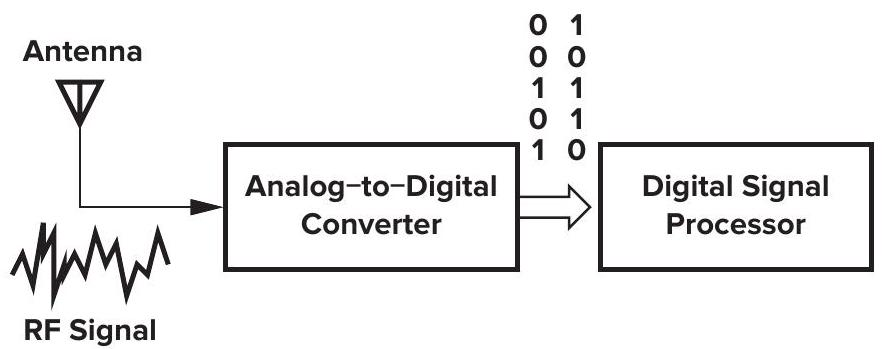
\includegraphics[max width=\textwidth, center]{2024_10_28_134d5d788a0919ac264dg-001}

Figure 1.1 Hypothetical RF receiver with direct signal digitization.

The answer is an emphatic no. An ADC that could digitize the minuscule RF signal ${ }^{1}$ would consume much more power than today's cell phone receivers. Furthermore, even if this approach were seriously considered, only analog designers would be able to develop the ADC. The key point offered by this example is that the sensing interface still demands high-performance analog design.\\
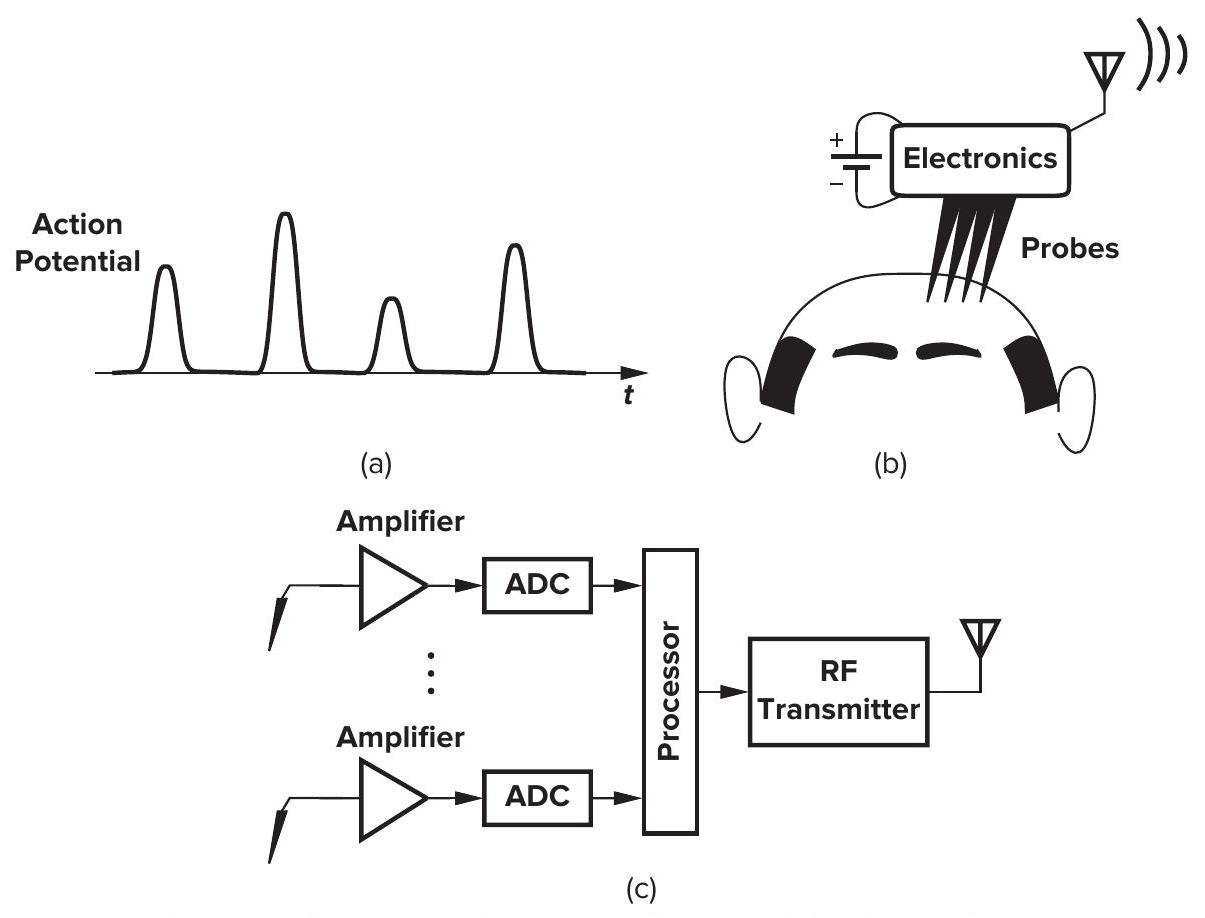
\includegraphics[max width=\textwidth, center]{2024_10_28_134d5d788a0919ac264dg-002}

Figure 1.2 (a) Voltage waveform generated as a result of neural activity, (b) use of probes to measure action potentials, and (c) processing and transmission of signals.

Another interesting example of sensing challenges arises in the study of the brain signals. Each time a neuron in your brain "fires," it generates an electric pulse with a height of a few millivolts and a duration of a few hundred microseconds [Fig. 1.2(a)]. To monitor brain activities, a neural recording system may employ tens of "probes" (electrodes) [Fig. 1.2(b)], each sensing a series of pulses. The signal produced by each probe must now be amplified, digitized, and transmitted wirelessly so that the patient is free to move around [Fig. 1.2(c)]. The sensing, processing, and transmission electronics in this environment must consume a low amount of power for two reasons: (1) to permit the use of a small battery for days or weeks, and (2) to minimize the rise in the chip's temperature, which could otherwise damage the patient's tissue. Among the functions shown in Fig. 1.2(c), the amplifiers, the ADCs, and the RF transmitter-all analog circuits-consume most of the power.

\subsection*{1.1.2 When Digital Signals Become Analog}
The use of analog circuits is not limited to analog signals. If a digital signal is so small and/or so distorted that a digital gate cannot interpret it correctly, then the analog designer must step in. For example, consider a long USB cable carrying data rate of hundreds of megabits per second between two laptops. As shown in Fig. 1.3, Laptop 1 delivers the data to the cable in the form of a sequence of ONEs and ZERO.

\footnotetext{${ }^{1}$ And withstand large unwanted signals.
}
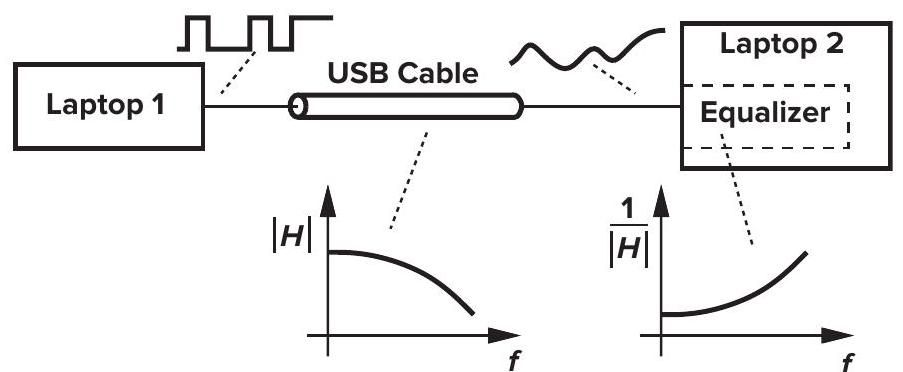
\includegraphics[max width=\textwidth, center]{2024_10_28_134d5d788a0919ac264dg-003}

Figure 1.3 Equalization to compensate for high-frequency attenuation in a USB cable.\\
Unfortunately, the cable exhibits a finite bandwidth, attenuating high frequencies and distorting the data as it reaches Laptop 2. This device must now perform sensing and processing, the former requiring an analog circuit (called an "equalizer") that corrects the distortion. For example, since the cable attenuates high frequencies, we may design the equalizer to amplify such frequencies, as shown conceptually by the $1 /|H|$ plot in Fig. 1.3.

The reader may wonder whether the task of equalization in Fig. 1.3 could be performed in the digital domain. That is, could we directly digitize the received distorted signal, digitally correct for the cable's limited bandwidth, and then carry out the standard USB signal processing? Indeed, this is possible if the ADC required here demands less power and less complexity than the analog equalizer. Following a detailed analysis, the analog designer decides which approach to adopt, but we intuitively know that at very high data rates, e.g., tens of gigabits per second, an analog equalizer proves more efficient than an ADC.

The above equalization task exemplifies a general trend in electronics: at lower speeds, it is more efficient to digitize the signal and perform the required function(s) in the digital domain, whereas at higher speeds, we implement the function(s) in the analog domain. The speed boundary between these two paradigms depends on the nature of the problem, but it has risen over time.

\subsection*{1.1.3 Analog Design Is in Great Demand}
Despite tremendous advances in semiconductor technology, analog design continues to face new challenges, thus calling for innovations. As a gauge of the demand for analog circuits, we can consider the papers published by industry and academia at circuits conferences and see what percentage fall in our domain. Figure 1.4 plots the number of analog papers published at the International Solid-State Circuits\\
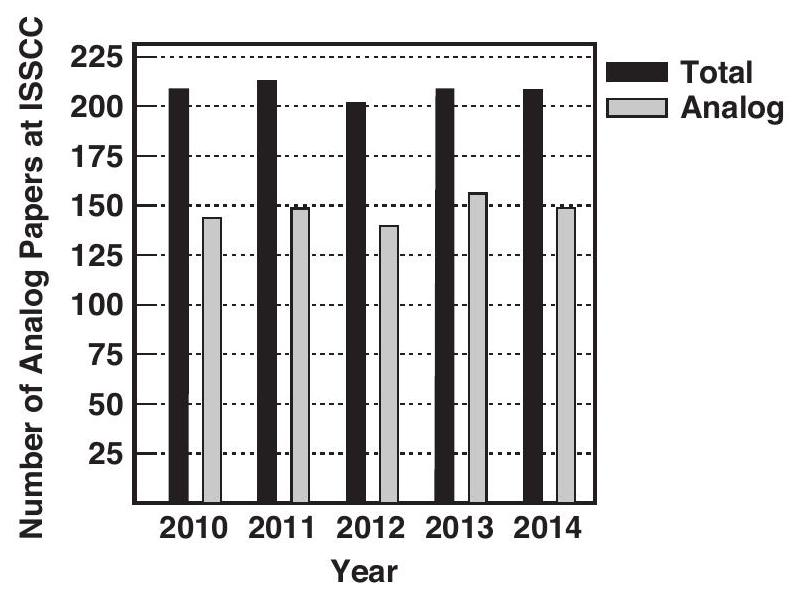
\includegraphics[max width=\textwidth, center]{2024_10_28_134d5d788a0919ac264dg-003(1)}

Figure 1.4 Number of analog papers published at the ISSCC in recent years.

Conference (ISSCC) in recent years, where "analog" is defined as a paper requiring the knowledge in this book. We observe that the majority of the papers involve analog design. This is true even though analog circuits are typically quite a lot less complex than digital circuits; an ADC contains several thousand transistors whereas a microprocessor employs billions.

\subsection*{1.1.4 Analog Design Challenges}
Today's analog designers must deal with interesting and difficult problems. Our study of devices and circuits in this book will systematically illustrate various issues, but it is helpful to take a brief look at what lies ahead.

Transistor Imperfections As a result of scaling, MOS transistors continue to become faster, but at the cost of their "analog" properties. For example, the maximum voltage gain that a transistor can provide declines with each new generation of CMOS technology. Moreover, a transistor's characteristics may depend on its surroundings, i.e., the size, shape, and distance of other components around it on the chip.

Declining Supply Voltages As a result of device scaling, the supply voltage of CMOS circuits has inevitably fallen from about 12 V in the 1970 s to about 0.9 V today. Many circuit configurations have not survived this supply reduction and have been discarded. We continue to seek new topologies that operate well at low voltages.

Power Consumption The semiconductor industry, more than ever, is striving for low-power design. This effort applies both to portable devices-so as to increase their battery lifetime-and to larger systems-so as to reduce the cost of heat removal and ease their drag on the earth's resources. MOS device scaling directly lowers the power consumption of digital circuits, but its effect on analog circuits is much more complicated.

Circuit Complexity Today's analog circuits may contain tens of thousands of transistors, demanding long and tedious simulations. Indeed, modern analog designers must be as adept at SPICE as at higherlevel simulators such as MATLAB.

PVT Variations Many device and circuit parameters vary with the fabrication process, supply voltage, and ambient temperature. We denote these effects by PVT and design circuits such that their performance is acceptable for a specified range of PVT variations. For example, the supply voltage may vary from 1 V to 0.95 V and the temperature from $0^{\circ}$ to $80^{\circ}$. Robust analog design in CMOS technology is a challenging task because device parameters vary significantly across PVT.

\section*{1.2 ■ Why Integrated?}
The idea of placing multiple electronic devices on the same substrate was conceived in the late 1950s. In 60 years, the technology has evolved from producing simple chips containing a handful of components to fabricating flash drives with one trillion transistors as well as microprocessors comprising several billion devices. As Gordon Moore (one of the founders of Intel) predicted in the early 1970s, the number of transistors per chip has continued to double approximately every one and a half years. At the same time, the minimum dimension of transistors has dropped from about $25 \mu \mathrm{~m}$ in 1960 to about 12 nm in the year 2015, resulting in a tremendous improvement in the speed of integrated circuits.

Driven primarily by the memory and microprocessor market, integrated-circuit technologies have also embraced analog design, affording a complexity, speed, and precision that would be impossible to achieve using discrete implementations. We can no longer build a discrete prototype to predict the behavior and performance of modern analog circuits.

\section*{1.3 ■ Why CMOS?}
The idea of metal-oxide-silicon field-effect transistors (MOSFETs) was patented by J. E. Lilienfeld in the early 1930s-well before the invention of the bipolar transistor. Owing to fabrication limitations, however, MOS technologies became practical only much later, in the early 1960s, with the first several generations producing only $n$-type transistors. It was in the mid-1960s that complementary MOS (CMOS) devices (i.e., with both $n$-type and $p$-type transistors) were introduced, initiating a revolution in the semiconductor industry.

CMOS technologies rapidly captured the digital market: CMOS gates dissipated power only during switching and required very few devices, two attributes in sharp contrast to their bipolar or GaAs counterparts. It was also soon discovered that the dimensions of MOS devices could be scaled down more easily than those of other types of transistors.

The next obvious step was to apply CMOS technology to analog design. The low cost of fabrication and the possibility of placing both analog and digital circuits on the same chip so as to improve the overall performance and/or reduce the cost of packaging made CMOS technology attractive. However, MOSFETs were slower and noisier than bipolar transistors, finding limited application.

How did CMOS technology come to dominate the analog market as well? The principal force was device scaling because it continued to improve the speed of MOSFETs. The intrinsic speed of MOS transistors has increased by orders of magnitude in the past 60 years, exceeding that of bipolar devices even though the latter have also been scaled (but not as fast).

Another critical advantage of MOS devices over bipolar transistors is that the former can operate with lower supply voltages. In today's technology, CMOS circuits run from supplies around 1 V and bipolar circuits around 2 V . The lower supplies have permitted a smaller power consumption for complex integrated circuits.

\section*{1.4 ■ Why This Book?}
The design of analog circuits itself has evolved together with the technology and the performance requirements. As the device dimensions shrink, the supply voltage of intergrated circuits drops, and analog and digital circuits are fabricated on one chip, many design issues arise that were previously unimportant. Such trends demand that the analysis and design of circuits be accompanied by an in-depth understanding of new technology-imposed limitations.

Good analog design requires intuition, rigor, and creativity. As analog designers, we must wear our engineer's hat for a quick and intuitive understanding of a large circuit, our mathematician's hat for quantifying subtle, yet important effects in a circuit, and our artist's hat for inventing new circuit topologies.

This book describes modern analog design from both intuitive and rigorous angles. It also fosters the reader's creativity by carefully guiding him or her through the evolution of each circuit and presenting the thought process that occurs during the development of new circuit techniques.

\section*{1.5 ■ Levels of Abstraction}
Analysis and design of integrated circuits often require thinking at various levels of abstraction. Depending on the effect or quantity of interest, we may study a complex circuit at device physics level, transistor level, architecture level, or system level. In other words, we may consider the behavior of individual devices in terms of their internal electric fields and charge transport [Fig. 1.5(a)], the interaction of a group of devices according to their electrical characteristics [Fig. 1.5(b)], the function of several building blocks operating as a unit [Fig. 1.5(c)], or the performance of the system in terms of that of its constituent subsystems\\
[Fig. 1.5(d)]. Switching between levels of abstraction becomes necessary in both understanding the details of the operation and optimizing the overall performance. In fact, in today's IC industry, the interaction among all groups, from device physicists to system designers, is essential to achieving high performance and low cost. In this book, we begin with device physics and develop increasingly more complex circuit topologies.\\
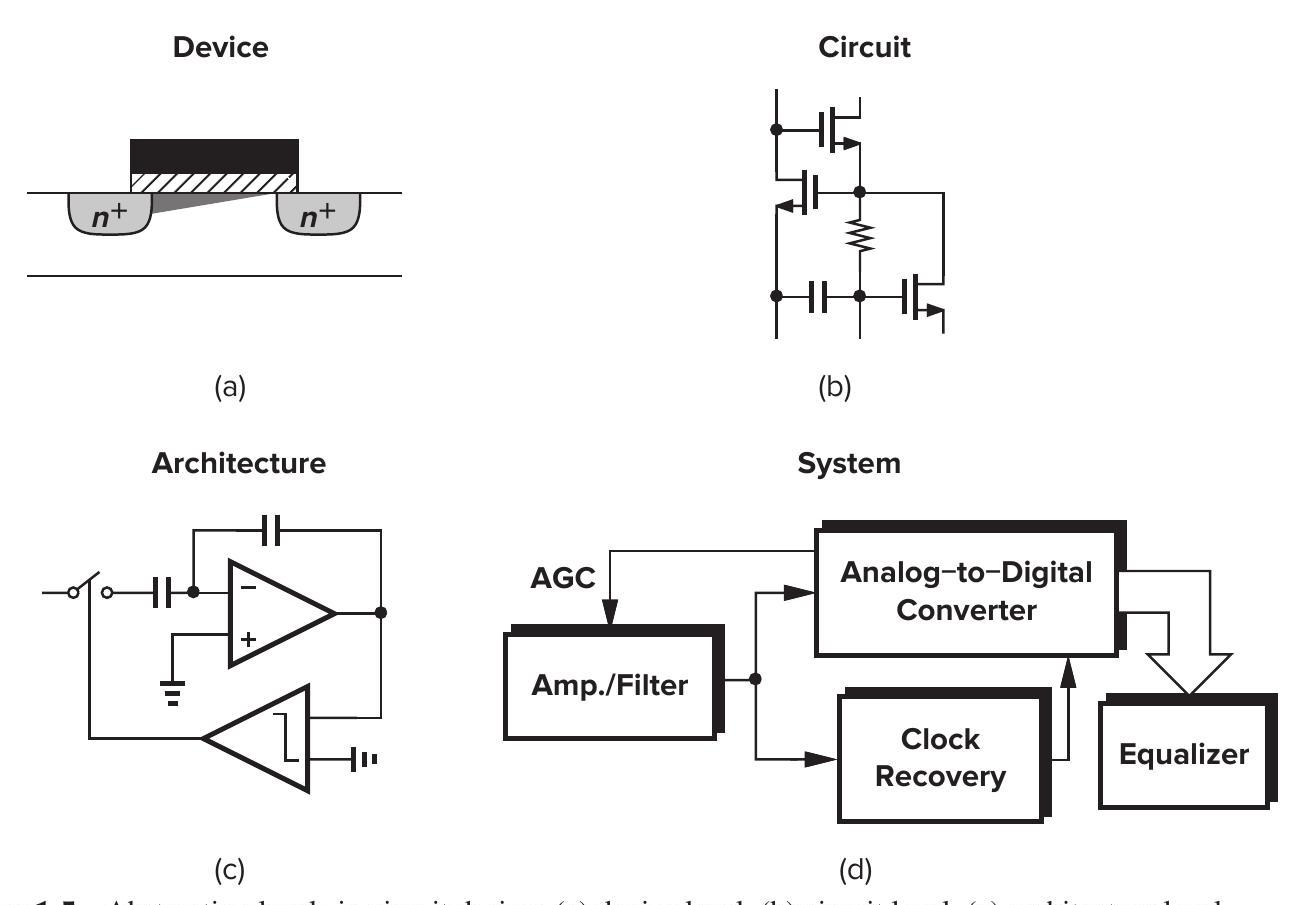
\includegraphics[max width=\textwidth, center]{2024_10_28_134d5d788a0919ac264dg-006}

Figure 1.5 Abstraction levels in circuit design: (a) device level, (b) circuit level, (c) architecture level, (d) system level.

\section*{CHAPTER 2}
\section*{Basic MOS Device Physics}
In studying the design of integrated circuits (ICs), one of two extreme approaches can be taken, (1) begin with quantum mechanics and understand solid-state physics, semiconductor device physics, device modeling, and finally the design of circuits; or (2) treat each semiconductor device as a black box whose behavior is described in terms of its terminal voltages and currents and design circuits with little attention to the internal operation of the device. Experience shows that neither approach is optimum. In the first case, the reader cannot see the relevance of all the physics to designing circuits, and in the second, he or she is constantly mystified by the contents of the black box.

In today's IC industry, a solid understanding of semiconductor devices is essential—more so in analog design than in digital design, because in the former, transistors are not considered to be simple switches, and many of their second-order effects directly impact the performance. Furthermore, as each new generation of IC technologies scales the devices, these effects become more significant. Since the designer must often decide which effects can be neglected in a given circuit, insight into device operation proves invaluable.

In this chapter, we study the physics of MOSFETs at an elementary level, covering the bare minimum that is necessary for basic analog design. The ultimate goal is still to develop a circuit model for each device by formulating its operation, but this is accomplished through a good understanding of the underlying principles. After studying many analog circuits in Chapters 3 through 14 and gaining motivation for a deeper understanding of devices, we return to the subject in Chapter 17 and deal with other aspects of MOS operation.

We begin our study with the structure of MOS transistors and derive their I/V characteristics. Next, we describe second-order effects such as body effect, channel-length modulation, and subthreshold conduction. We then identify the parasitic capacitances of MOSFETs, derive a small-signal model, and present a simple SPICE model. We assume that the reader is familiar with such basic concepts as doping, mobility, and $p n$ junctions.

\section*{2.1 ■ General Considerations}
\subsection*{2.1.1 MOSFET as a Switch}
Before delving into the actual operation of the MOSFET, we consider a simplistic model of the device so as to gain a feel for what the transistor is expected to be and which aspects of its behavior are important.

Shown in Fig. 2.1 is the symbol for an $n$-type MOSFET, revealing three terminals: gate (G), source (S), and drain (D). The latter two are interchangeable because the device is symmetric. When operating\\
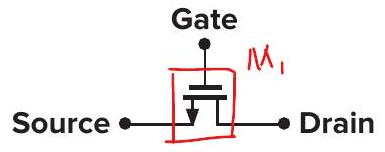
\includegraphics[max width=\textwidth, center]{2024_10_28_134d5d788a0919ac264dg-008}

Figure 2.1 Simple view of a MOS device.\\
as a switch, the transistor "connects" the source and the drain together if the gate voltage, $V_{G}$, is "high" and isolates the source and the drain if $V_{G}$ is "low."

Even with this simplified view, we must answer several questions. For what value of $V_{G}$ does the device turn on? In other words, what is the "threshold" voltage? What is the resistance between S and D when the device is on (or off)? How does this resistance depend on the terminal voltages? Can we always model the path between S and D by a simple linear resistor? What limits the speed of the device?

While all of these questions arise at the circuit level, they can be answered only by analyzing the structure and physics of the transistor.

\subsection*{2.1.2 MOSFET Structure}
Figure 2.2 shows a simplified structure of an $n$-type MOS (NMOS) device. Fabricated on a $p$-type substrate (also called the "bulk" or the "body"), the device consists of two heavily-doped $n$ regions forming the source and drain terminals, a heavily-doped (conductive) piece of polysilicon ${ }^{1}$ (simply called "poly") operating as the gate, and a thin layer of silicon dioxide $\left(\mathrm{SiO}_{2}\right)$ (simply called "oxide") insulating the gate from the substrate. The useful action of the device occurs in the substrate region under the gate oxide. Note that the structure is symmetric with respect to S and D .\\
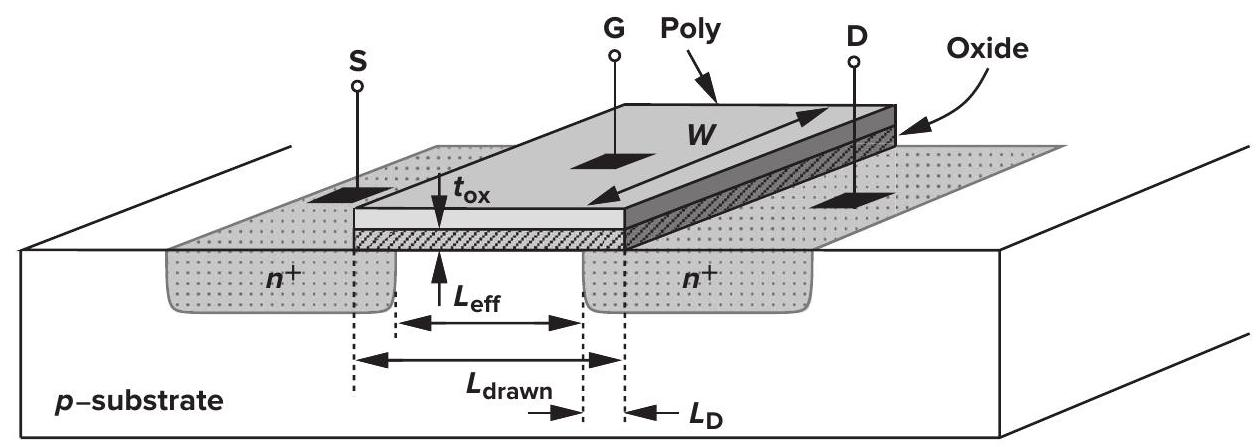
\includegraphics[max width=\textwidth, center]{2024_10_28_134d5d788a0919ac264dg-008(1)}

Figure 2.2 Structure of a MOS device.\\
The lateral dimension of the gate along the source-drain path is called the length, $L$, and that perpendicular to the length is called the width, $W$. Since the S/D junctions "side-diffuse" during fabrication, the actual distance between the source and the drain is slightly less than $L$. To avoid confusion, we write, $L_{\text {eff }}=L_{\text {drawn }}-2 L_{D}$, where $L_{\text {eff }}$ is the "effective" length, $L_{\text {drawn }}$ is the total length, ${ }^{2}$ and $L_{D}$ is the amount of side diffusion. As we will see later, $L_{e f f}$ and the gate oxide thickness, $t_{o x}$, play an important role in the performance of MOS circuits. Consequently, the principal thrust in MOS technology development is to reduce both of these dimensions from one generation to the next without degrading other parameters of the device. Typical values at the time of this writing are $L_{e f f} \approx 10 \mathrm{~nm}$ and $t_{o x} \approx 15 \AA$. In the remainder of this book, we denote the effective length by $L$ unless otherwise stated.

\footnotetext{${ }^{1}$ Polysilicon is silicon in amorphous (non crystal) form. As explained in Chapter 18, when the gate silicon is grown on top of the oxide, it cannot form a crystal. The gate was originally made of metal [hence the term "metal-oxide-semiconductor" (MOS)] and is returning to metal in recent generations.\\
${ }^{2}$ The subscript "drawn" is used because this is the dimension that we draw in the layout of the transistor (Sec. 2.4.1).
}If the MOS structure is symmetric, why do we call one $n$ region the source and the other the drain? This becomes clear if the source is defined as the terminal that provides the charge carriers (electrons in the case of NMOS devices) and the drain as the terminal that collects them. Thus, as the voltages at the three terminals of the device vary, the source and the drain may exchange roles. These concepts are practiced in the problems at the end of the chapter.

We have thus far ignored the substrate on which the device is fabricated. In reality, the substrate potential greatly influences the device characteristics. That is, the MOSFET is a four-terminal device. Since in typical MOS operation, the S/D junction diodes must be reverse-biased, we assume that the substrate of NMOS transistors is connected to the most negative supply in the system. For example, if a circuit operates between zero and 1.2 volts, $V_{\text {sub,NMOS }}=0$. The actual connection is usually provided through an ohmic $p^{+}$region, as depicted in the side view of the device in Fig. 2.3.\\
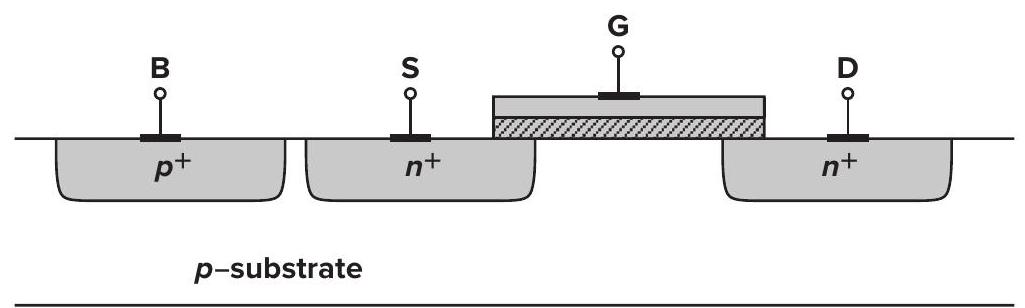
\includegraphics[max width=\textwidth, center]{2024_10_28_134d5d788a0919ac264dg-009}

Figure 2.3 Substrate connection.

In complementary MOS (CMOS) technologies, both NMOS and PMOS transistors are available. From a simplistic viewpoint, the PMOS device is obtained by negating all of the doping types (including the substrate) [Fig. 2.4(a)], but in practice, NMOS and PMOS devices must be fabricated on the same wafer, i.e., the same substrate. For this reason, one device type can be placed in a "local substrate," usually called a "well." In today's CMOS processes, the PMOS device is fabricated in an $n$-well [Fig. 2.4(b)]. Note that the $n$-well must be connected to a potential such that the S/D junction diodes of the PMOS transistor remain reverse-biased under all conditions. In most circuits, the $n$-well is tied to the most positive supply voltage. For the sake of brevity, we sometimes call NMOS and PMOS devices "NFETs" and "PFETs," respectively.

Figure 2.4(b) indicates an interesting difference between NMOS and PMOS transistors: while all NFETs share the same substrate, each PFET can have an independent $n$-well. This flexibility of PFETs is exploited in some analog circuits.

\subsection*{2.1.3 MOS Symbols}
The circuit symbols used to represent NMOS and PMOS transistors are shown in Fig. 2.5. The symbols in Fig. 2.5(a) contain all four terminals, with the substrate denoted by "B" (bulk) rather than " $S$ " to avoid confusion with the source. The source of the PMOS device is positioned on top as a visual aid because it has a higher potential than its gate. Since in most circuits the bulk terminals of NMOS and PMOS devices are tied to ground and $V_{D D}$, respectively, we usually omit these connections in drawing [Fig. 2.5(b)]. In digital circuits, it is customary to use the "switch" symbols depicted in Fig. 2.5(c) for the two types, but we prefer those in Fig. 2.5(b) because the visual distinction between S and D proves helpful in understanding the operation of circuits.

\section*{Nanometer Design Notes}
Some modern CMOS processes offer a "deep $n$-well," an $n$-well that contains an NMOS device and its $p$-type bulk. As shown below, the NMOS transistor's bulk is now localized and need not be tied to that of other NMOS devices. But the design incurs substantial area overhead because the deep $n$-well must extend beyond the $p$-well by a certain amount and must maintain a certain distance to the regular $n$-well.\\
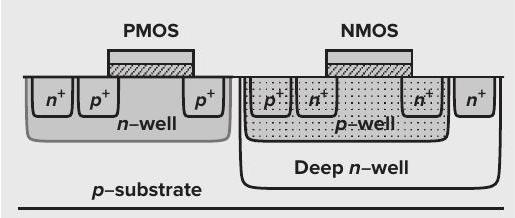
\includegraphics[max width=\textwidth, center]{2024_10_28_134d5d788a0919ac264dg-009(1)}\\
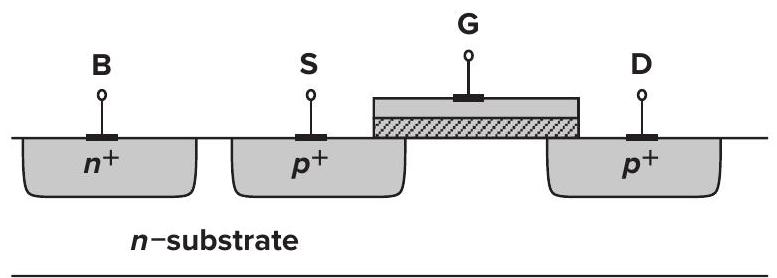
\includegraphics[max width=\textwidth, center]{2024_10_28_134d5d788a0919ac264dg-010(1)}\\
(a)\\
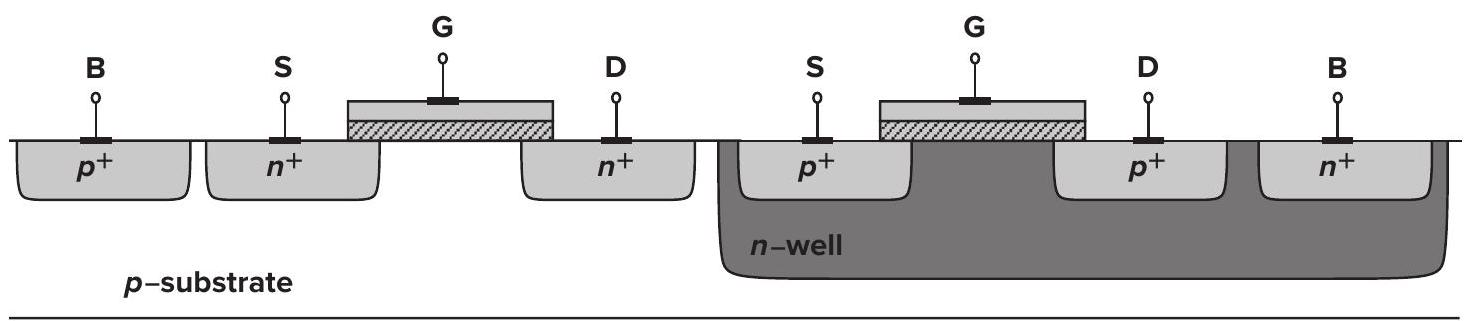
\includegraphics[max width=\textwidth, center]{2024_10_28_134d5d788a0919ac264dg-010(4)}\\
(b)\\
Figure 2.4 (a) Simple PMOS device; (b) PMOS inside an $n$-well.

NMOS\\
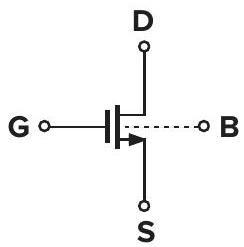
\includegraphics[max width=\textwidth, center]{2024_10_28_134d5d788a0919ac264dg-010(2)}

PMOS\\
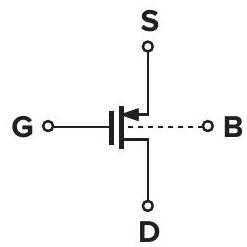
\includegraphics[max width=\textwidth, center]{2024_10_28_134d5d788a0919ac264dg-010(3)}\\
(a)\\
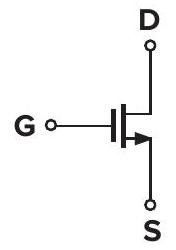
\includegraphics[max width=\textwidth, center]{2024_10_28_134d5d788a0919ac264dg-010}\\
(b)\\
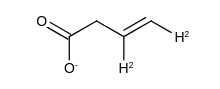
\includegraphics{smile-a955b526b036de8cce5deb8dc1583a9164f722fb}\\
(c)

Figure 2.5 MOS symbols.

\section*{2.2 ■ MOS I/V Characteristics}
In this section, we analyze the generation and transport of charge in MOSFETs as a function of the terminal voltages. Our objective is to derive equations for the I/V characteristics such that we can elevate our abstraction from device physics level to circuit level.

\subsection*{2.2.1 Threshold Voltage}
Consider an NFET connected to external voltages as shown in Fig. 2.6(a). What happens as the gate voltage, $V_{G}$, increases from zero? Since the gate, the dielectric, and the substrate form a capacitor, as $V_{G}$ becomes more positive, the holes in the $p$-substrate are repelled from the gate area, leaving negative ions behind so as to mirror the charge on the gate. In other words, a depletion region is created [Fig. 2.6(b)]. Under this condition, no current flows because no charge carriers are available.

As $V_{G}$ increases, so do the width of the depletion region and the potential at the oxide-silicon interface. In a sense, the structure resembles a voltage divider consisting of two capacitors in series: the gateoxide capacitor and the depletion-region capacitor [Fig. 2.6(c)]. When the interface potential reaches a sufficiently positive value, electrons flow from the source to the interface and eventually to the drain.\\
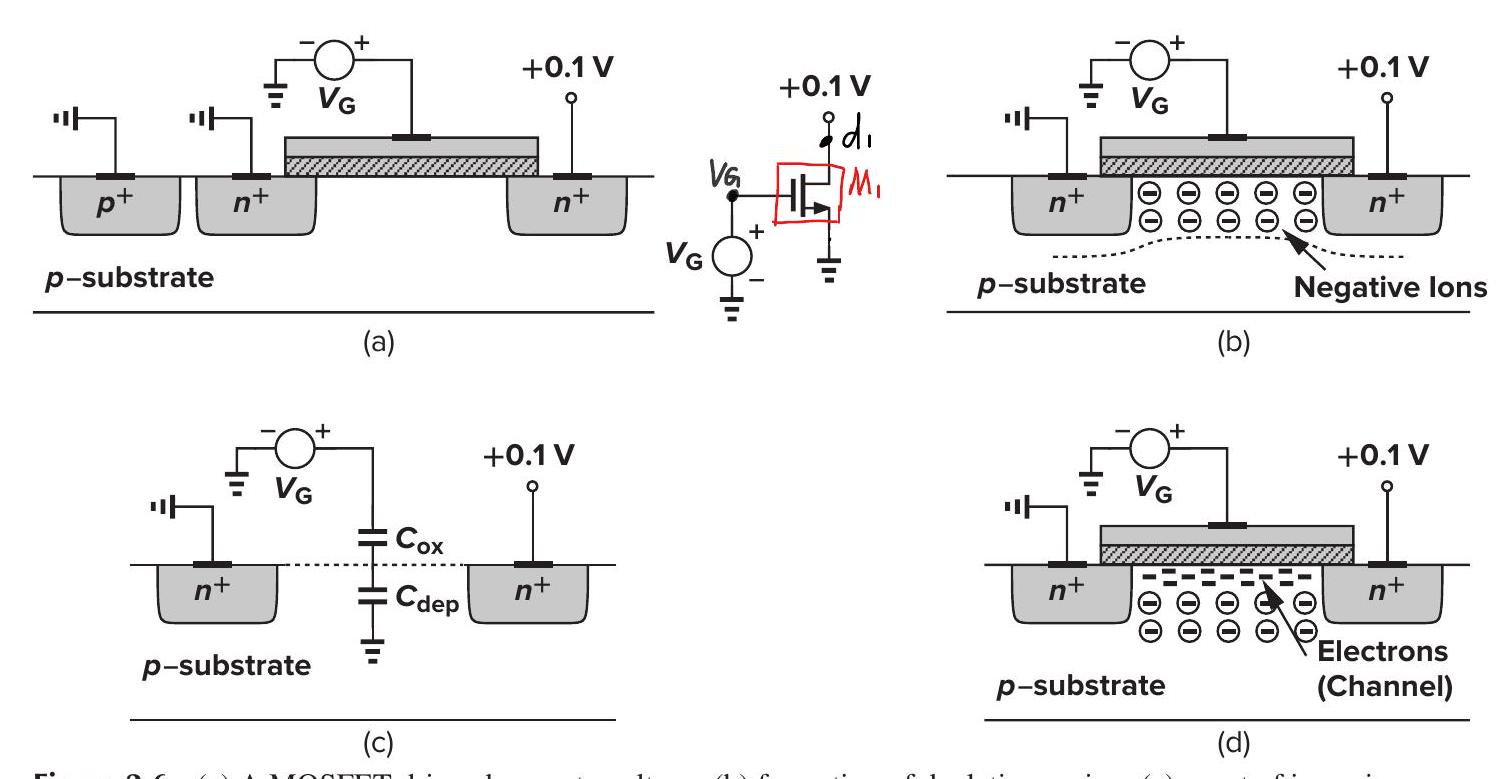
\includegraphics[max width=\textwidth, center]{2024_10_28_134d5d788a0919ac264dg-011}

Figure 2.6 (a) A MOSFET driven by a gate voltage; (b) formation of depletion region; (c) onset of inversion; (d) formation of inversion layer.

Thus, a "channel" of charge carriers is formed under the gate oxide between S and D , and the transistor is "turned on." We say the interface is "inverted." For this reason, the channel is also called the "inversion layer." The value of $V_{G}$ for which this occurs is called the "threshold voltage," $V_{T H}$. If $V_{G}$ rises further, the charge in the depletion region remains relatively constant while the channel charge density continues to increase, providing a greater current from S to D .

In reality, the turn-on phenomenon is a gradual function of the gate voltage, making it difficult to define $V_{T H}$ unambiguously. In semiconductor physics, the $V_{T H}$ of an NFET is usually defined as the gate voltage for which the interface is "as much $n$-type as the substrate is $p$-type." It can be proved [1] that $^{3}$


\begin{equation*}
V_{T H}=\Phi_{M S}+2 \Phi_{F}+\frac{Q_{d e p}}{C_{o x}} \tag{2.1}
\end{equation*}


where $\Phi_{M S}$ is the difference between the work functions of the polysilicon gate and the silicon substrate, $\Phi_{F}=(k T / q) \ln \left(N_{\text {sub }} / n_{i}\right), k$ is Boltzmann's constant, $q$ is the electron charge, $N_{\text {sub }}$ is the doping density of the substrate, $n_{i}$ is the density of electrons in undoped silicon, $Q_{d e p}$ is the charge in the depletion region, and $C_{o x}$ is the gate-oxide capacitance per unit area. From $p n$ junction theory, $Q_{d e p}=\sqrt{4 q \epsilon_{s i}\left|\Phi_{F}\right| N_{s u b}}$, where $\epsilon_{s i}$ denotes the dielectric constant of silicon. Since $C_{o x}$ appears very frequently in device and circuit calculations, it is helpful to remember that for $t_{o x} \approx 20 \AA, C_{o x} \approx 17.25 \mathrm{fF} / \mu \mathrm{m}^{2}$. The value of $C_{o x}$ can then be scaled proportionally for other oxide thicknesses.

In practice, the "native" threshold value obtained from the above equation may not be suited to circuit design, e.g., $V_{T H}=0$ and the device does not turn off for $V_{G} \geq 0 .{ }^{4}$ For this reason, the threshold voltage is typically adjusted by implantation of dopants into the channel area during device fabrication, in essence altering the doping level of the substrate near the oxide interface. For example, as shown in Fig. 2.7, if a thin sheet of $p^{+}$is created, the gate voltage required to deplete this region increases.

\footnotetext{${ }^{3}$ Charge trapping in the oxide is neglected here.\\
${ }^{4}$ Called a "depletion-mode" FET, such a device was used in old technologies. NFETs with a positive threshold are called "enhancement-mode" devices.
}
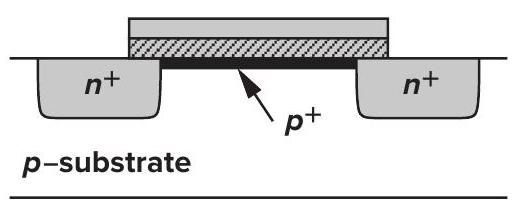
\includegraphics[max width=\textwidth, center]{2024_10_28_134d5d788a0919ac264dg-012}

Figure 2.7 Implantation of $p+$ dopants to alter the threshold.

The above definition is not directly applicable to the measurement of $V_{T H}$. In Fig. 2.6(a), only the drain current can indicate whether the device is "on" or "off," failing to reveal at what $V_{G S}$ the interface is as much $n$-type as the bulk is $p$-type. As a result, the calculation of $V_{T H}$ from I/V measurements is somewhat ambiguous. We will return to this point later, but assume for now that the device turns on abruptly for $V_{G S} \geq V_{T H}$.

The turn-on phenomenon in a PMOS device is similar to that of NFETs, but with all the polarities reversed. As shown in Fig. 2.8, if the gate-source voltage becomes sufficiently negative, an inversion layer consisting of holes is formed at the oxide-silicon interface, providing a conduction path between the source and the drain. That is, the threshold voltage of a PMOS device is typically negative.\\
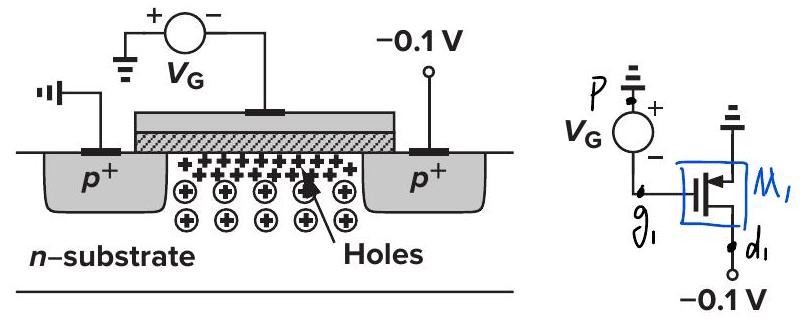
\includegraphics[max width=\textwidth, center]{2024_10_28_134d5d788a0919ac264dg-012(2)}

Figure 2.8 Formation of inversion layer in a PFET.

\subsection*{2.2.2 Derivation of I/V Characteristics}
In order to obtain the relationship between the drain current of a MOSFET and its terminal voltages, we make two observations.

First, consider a semiconductor bar carrying a current $I$ [Fig. 2.9(a)]. If the mobile charge density along the direction of current is $Q_{d}$ coulombs per meter and the velocity of the charge is $v$ meters per second, then


\begin{equation*}
I=Q_{d} \cdot v \tag{2.2}
\end{equation*}


To understand why, we measure the total charge that passes through a cross section of the bar in unit time. With a velocity $v$, all of the charge enclosed in $v$ meters of the bar must flow through the cross section in\\
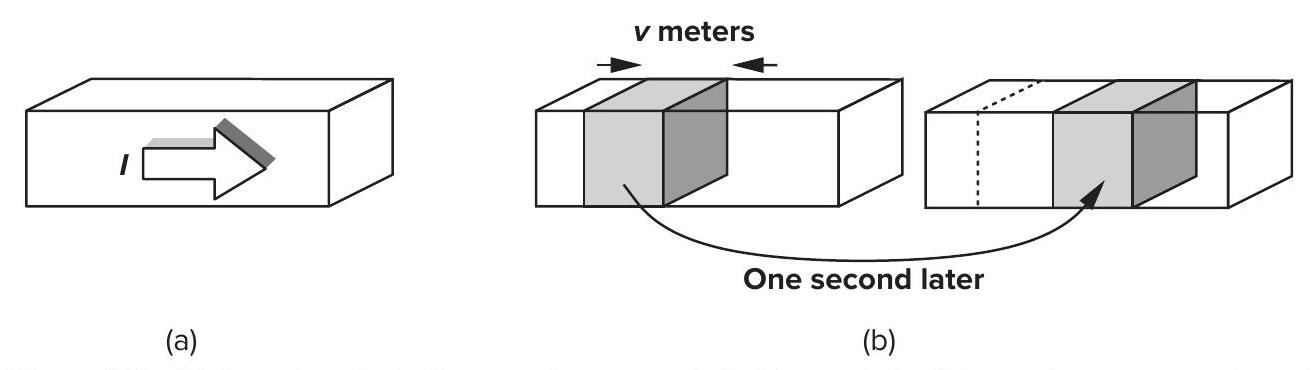
\includegraphics[max width=\textwidth, center]{2024_10_28_134d5d788a0919ac264dg-012(1)}

Figure 2.9 (a) A semiconductor bar carrying a current $I$; (b) snapshots of the carriers one second apart.\\
one second [Fig. 2.9(b)]. Since the charge density is $Q_{d}$, the total charge in $v$ meters equals $Q_{d} \cdot v$. This lemma proves useful in analyzing semiconductor devices.

Second, to utilize the above lemma, we must determine the mobile charge density in a MOSFET. To this end, consider an NFET whose source and drain are connected to ground [Fig. 2.10(a)]. What is the charge density in the inversion layer? Since we assume that the onset of inversion occurs at $V_{G S}=V_{T H}$, the inversion charge density produced by the gate-oxide capacitance is proportional to $V_{G S}-V_{T H}$. For $V_{G S} \geq V_{T H}$, any charge placed on the gate must be mirrored by the charge in the channel, yielding a uniform channel charge density (charge per unit length along the source-drain path) equal to


\begin{equation*}
Q_{d}=W C_{o x}\left(V_{G S}-V_{T H}\right) \tag{2.3}
\end{equation*}


where $C_{o x}$ is multiplied by $W$ to represent the total capacitance per unit length.\\
Now suppose, as depicted in Fig. 2.10(b), that the drain voltage is greater than zero. Since the channel potential varies from zero at the source to $V_{D}$ at the drain, the local voltage difference between the gate and the channel varies from $V_{G}$ (near the source) to $V_{G}-V_{D}$ (near the drain). Thus, the charge density at a point $x$ along the channel can be written as


\begin{equation*}
Q_{d}(x)=W C_{o x}\left[V_{G S}-V(x)-V_{T H}\right] \tag{2.4}
\end{equation*}


where $V(x)$ is the channel potential at $x$. From (2.2), the current is given by


\begin{equation*}
I_{D}=-W C_{o x}\left[V_{G S}-V(x)-V_{T H}\right] v \tag{2.5}
\end{equation*}


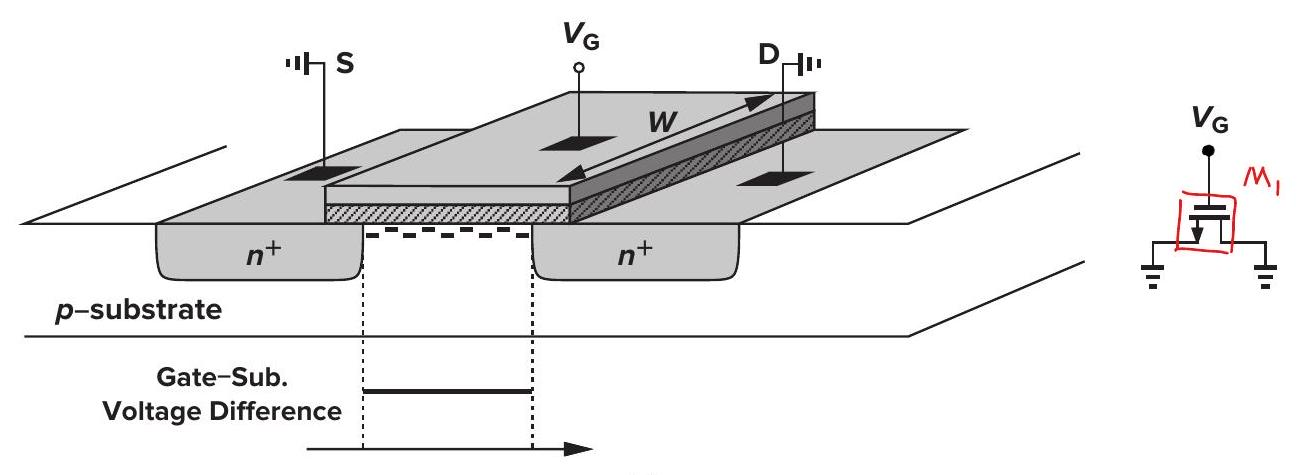
\includegraphics[max width=\textwidth, center]{2024_10_28_134d5d788a0919ac264dg-013}\\
(a)\\
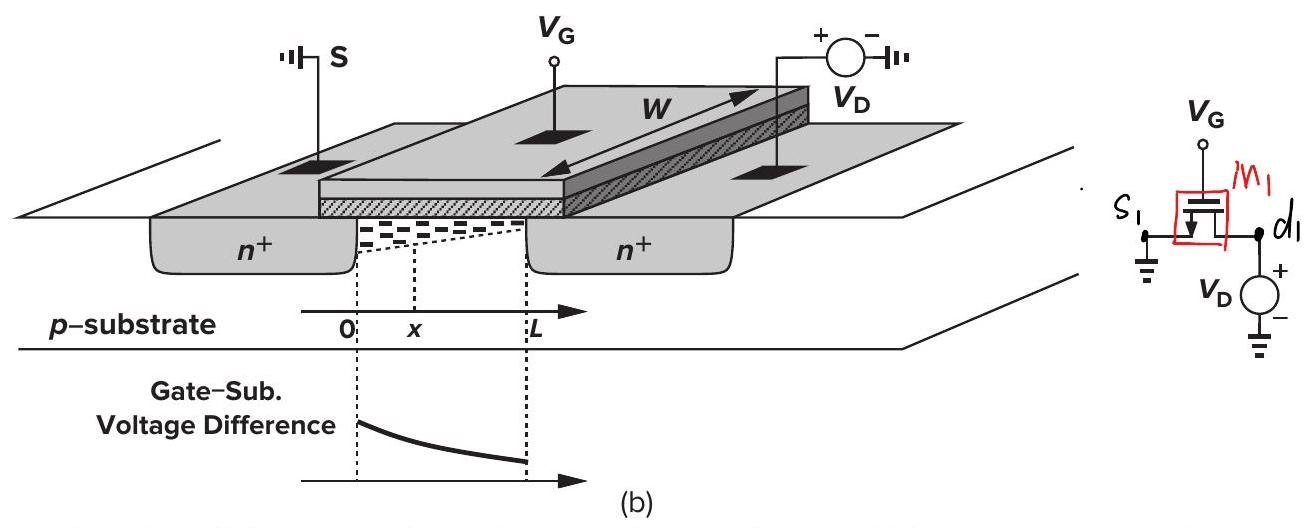
\includegraphics[max width=\textwidth, center]{2024_10_28_134d5d788a0919ac264dg-013(1)}

Figure 2.10 Channel charge with (a) equal source and drain voltages and (b) unequal source and drain voltages.\\
where the negative sign is inserted because the charge carriers are negative. Note that $v$ denotes the velocity of the electrons in the channel. For semiconductors, $v=\mu E$, where $\mu$ is the mobility of charge carriers and $E$ is the electric field. Noting that $E(x)=-d V / d x$ and representing the mobility of electrons by $\mu_{n}$, we have


\begin{equation*}
I_{D}=W C_{o x}\left[V_{G S}-V(x)-V_{T H}\right] \mu_{n} \frac{d V(x)}{d x} \tag{2.6}
\end{equation*}


subject to boundary conditions $V(0)=0$ and $V(L)=V_{D S}$. While $V(x)$ can be easily found from this equation, the quantity of interest is in fact $I_{D}$. Multiplying both sides by $d x$ and performing integration, we obtain


\begin{equation*}
\int_{x=0}^{L} I_{D} d x=\int_{V=0}^{V_{D S}} W C_{o x} \mu_{n}\left[V_{G S}-V(x)-V_{T H}\right] d V \tag{2.7}
\end{equation*}


Since $I_{D}$ is constant along the channel,


\begin{equation*}
I_{D}=\mu_{n} C_{o x} \frac{W}{L}\left[\left(V_{G S}-V_{T H}\right) V_{D S}-\frac{1}{2} V_{D S}^{2}\right] \tag{2.8}
\end{equation*}


Note that $L$ is the effective channel length.\\
Figure 2.11 plots the parabolas given by (2.8) for different values of $V_{G S}$, indicating that the "current capability" of the device increases with $V_{G S}$. Calculating $\partial I_{D} / \partial V_{D S}$, the reader can show that the peak of each parabola occurs at $V_{D S}=V_{G S}-V_{T H}$ and the peak current is


\begin{equation*}
I_{D, \max }=\frac{1}{2} \mu_{n} C_{o x} \frac{W}{L}\left(V_{G S}-V_{T H}\right)^{2} \tag{2.9}
\end{equation*}


We call $V_{G S}-V_{T H}$ the "overdrive voltage" and $W / L$ the "aspect ratio." If $V_{D S} \leq V_{G S}-V_{T H}$, we say the device operates in the "triode region." 5\\
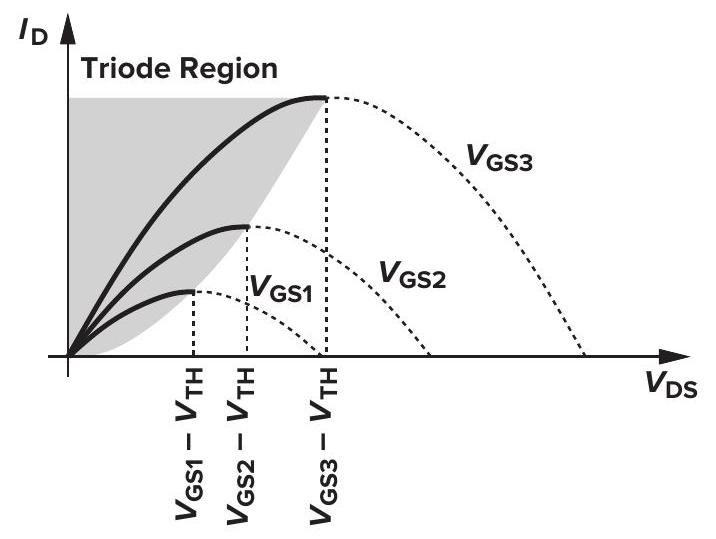
\includegraphics[max width=\textwidth, center]{2024_10_28_134d5d788a0919ac264dg-014}

Figure 2.11 Drain current versus drain-source voltage in the triode region.

Equations (2.8) and (2.9) serve as our first step toward CMOS circuit design, describing the dependence of $I_{D}$ upon the constant of the technology, $\mu_{n} C_{o x}$, the device dimensions, $W$ and $L$, and the gate and drain potentials with respect to the source. Note that the integration in (2.7) assumes that $\mu_{n}$ and $V_{T H}$ are independent of $x$ and the gate and drain voltages, an approximation that we will revisit in Chapter 17.

\footnotetext{${ }^{5}$ Also called the "linear region."
}If in (2.8), $V_{D S} \ll 2\left(V_{G S}-V_{T H}\right)$, we have


\begin{equation*}
I_{D} \approx \mu_{n} C_{o x} \frac{W}{L}\left(V_{G S}-V_{T H}\right) V_{D S} \tag{2.10}
\end{equation*}


that is, the drain current is a linear function of $V_{D S}$. This is also evident from the characteristics of Fig. 2.11 for small $V_{D S}$ : as shown in Fig. 2.12, each parabola can be approximated by a straight line. The linear relationship implies that the path from the source to the drain can be represented by a linear resistor equal to


\begin{equation*}
R_{o n}=\frac{1}{\mu_{n} C_{o x} \frac{W}{L}\left(V_{G S}-V_{T H}\right)} \tag{2.11}
\end{equation*}


\begin{center}
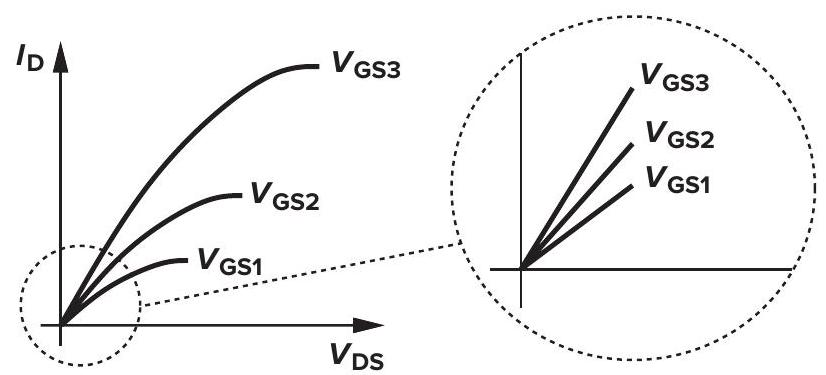
\includegraphics[max width=\textwidth]{2024_10_28_134d5d788a0919ac264dg-015}
\end{center}

Figure 2.12 Linear operation in deep triode region.\\
A MOSFET can therefore operate as a resistor whose value is controlled by the overdrive voltage [so long as $\left.V_{D S} \ll 2\left(V_{G S}-V_{T H}\right)\right]$. This is conceptually illustrated in Fig. 2.13. Note that in contrast to bipolar transistors, a MOS device may be on even if it carries no current. With the condition $V_{D S} \ll 2\left(V_{G S}-V_{T H}\right)$, we say the device operates in the deep triode region.\\
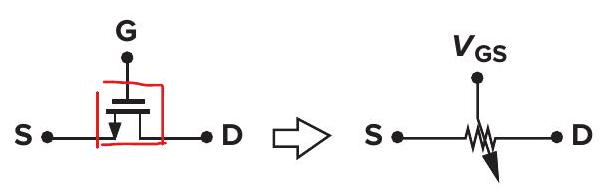
\includegraphics[max width=\textwidth, center]{2024_10_28_134d5d788a0919ac264dg-015(1)}

Figure 2.13 MOSFET as a controlled linear resistor.

\section*{Example 2.1}
For the arrangement in Fig. 2.14(a), plot the on-resistance of $M_{1}$ as a function of $V_{G}$. Assume that $\mu_{n} C_{o x}=$ $50 \mu \mathrm{~A} / \mathrm{V}^{2}, W / L=10$, and $V_{T H}=0.3 \mathrm{~V}$. Note that the drain terminal is open.

\section*{Solution}
Since the drain terminal is open, $I_{D}=0$ and $V_{D S}=0$. Thus, if the device is on, it operates in the deep triode region. For $V_{G}<1 \mathrm{~V}+V_{T H}, M_{1}$ is off and $R_{o n}=\infty$. For $V_{G}>1 \mathrm{~V}+V_{T H}$, we have


\begin{equation*}
R_{o n}=\frac{1}{50 \mu \mathrm{~A} / \mathrm{V}^{2} \times 10\left(V_{G}-1 \mathrm{~V}-0.3 \mathrm{~V}\right)} \tag{2.12}
\end{equation*}


The result is plotted in Fig. 2.14(b).\\
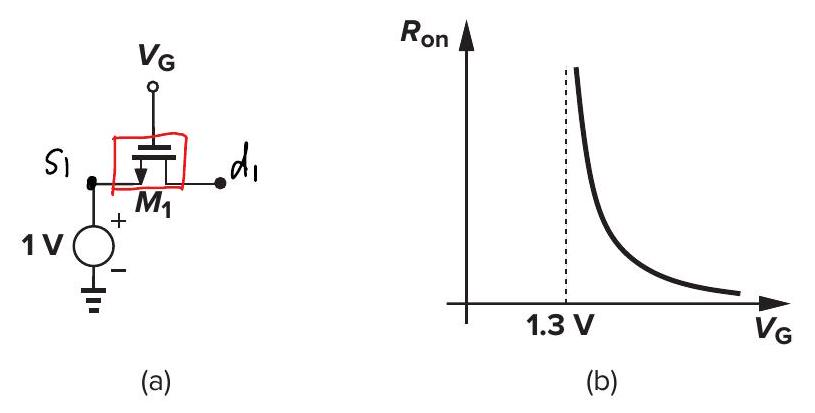
\includegraphics[max width=\textwidth, center]{2024_10_28_134d5d788a0919ac264dg-016(1)}

Figure 2.14

MOSFETs operating as controllable resistors play a crucial role in many analog circuits. For example, a voltage-controlled resistor can be used to adjust the frequency of the clock generator in a laptop computer if the system must go into a power saving mode. As studied in Chapter 13, MOSFETs also serve as switches.

What happens if the drain-source voltage in Fig. 2.11 exceeds $V_{G S}-V_{T H}$ ? In reality, the drain current does not follow the parabolic behavior for $V_{D S}>V_{G S}-V_{T H}$. In fact, as shown in Fig. 2.15, $I_{D}$ becomes relatively constant, and we say the device operates in the "saturation" region. ${ }^{6}$ To understand this phenomenon, recall from (2.4) that the local density of the inversion-layer charge is proportional to $V_{G S}-V(x)-V_{T H}$. Thus, if $V(x)$ approaches $V_{G S}-V_{T H}$, then $Q_{d}(x)$ drops to zero. In other words, as depicted in Fig. 2.16, if $V_{D S}$ is slightly greater than $V_{G S}-V_{T H}$, then the inversion layer stops at $x \leq L$, and we say the channel is "pinched off." As $V_{D S}$ increases further, the point at which $Q_{d}$ equals zero gradually moves toward the source. Thus, at some point along the channel, the local potential difference between the gate and the oxide-silicon interface is not sufficient to support an inversion layer.\\
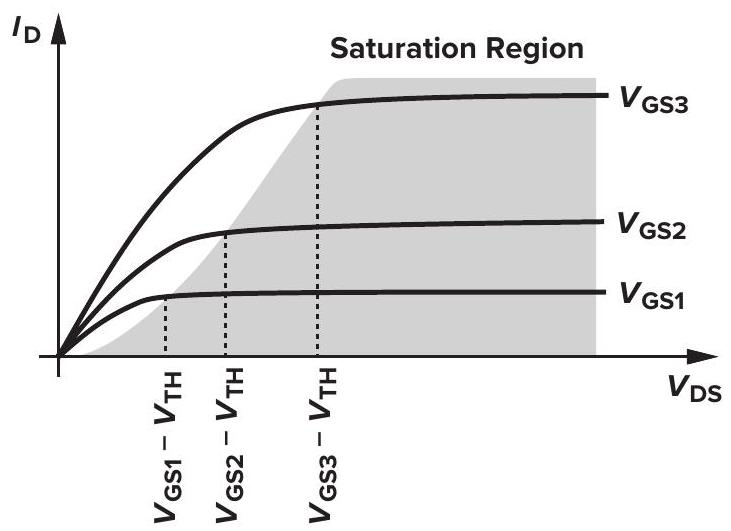
\includegraphics[max width=\textwidth, center]{2024_10_28_134d5d788a0919ac264dg-016}

Figure 2.15 Saturation of drain current.

How does the device conduct current in the presence of pinch-off? As the electrons approach the pinch-off point (where $Q_{d} \rightarrow 0$ ), their velocity rises tremendously ( $v=I / Q_{d}$ ). Upon passing the pinchoff point, the electrons simply shoot through the depletion region near the drain junction and arrive at the drain terminal.

\footnotetext{${ }^{6}$ Note the difference between saturation in bipolar and MOS devices.
}
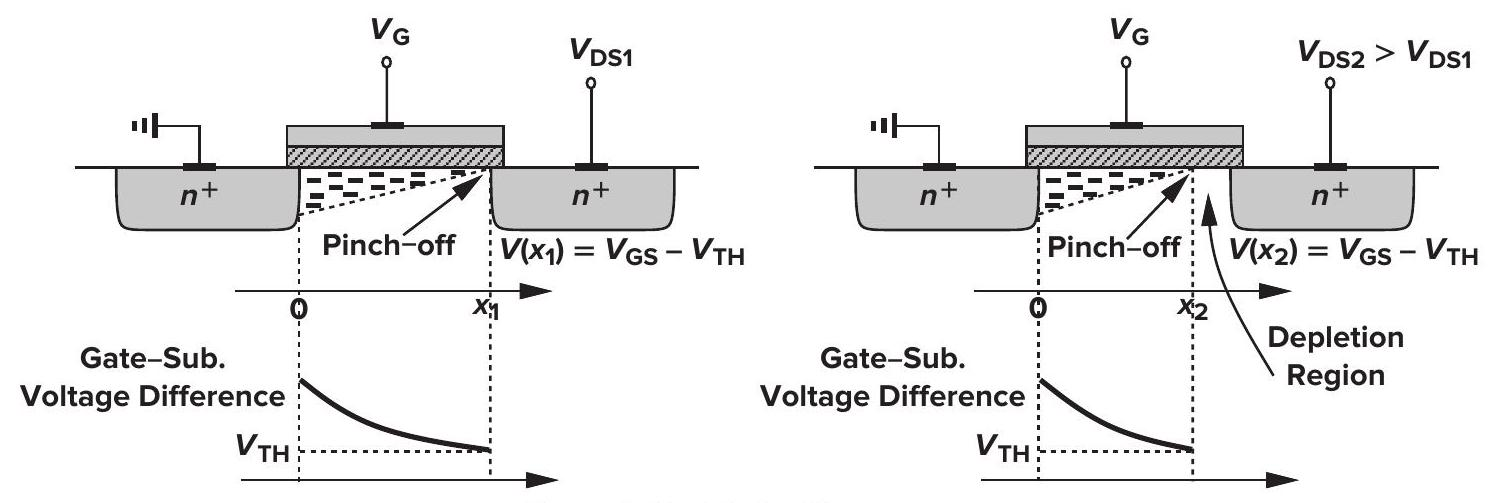
\includegraphics[max width=\textwidth, center]{2024_10_28_134d5d788a0919ac264dg-017}

Figure 2.16 Pinch-off behavior.

With the above observations, we reexamine (2.7) for a saturated device. Since $Q_{d}$ is the density of mobile charge, the integral on the left-hand side of (2.7) must be taken from $x=0$ to $x=L^{\prime}$, where $L^{\prime}$ is the point at which $Q_{d}$ drops to zero (e.g., $x_{2}$ in Fig. 2.16), and that on the right from $V(x)=0$ to $V(x)=V_{G S}-V_{T H}$. As a result,


\begin{equation*}
I_{D}=\frac{1}{2} \mu_{n} C_{o x} \frac{W}{L^{\prime}}\left(V_{G S}-V_{T H}\right)^{2} \tag{2.13}
\end{equation*}


indicating that $I_{D}$ is relatively independent of $V_{D S}$ if $L^{\prime}$ remains close to $L$. We say the device exhibits a "square-law" behavior. If $I_{D}$ is known, then $V_{G S}$ is obtained as


\begin{equation*}
V_{G S}=\sqrt{\frac{2 I_{D}}{\mu_{n} C_{o x} \frac{W}{L^{\prime}}}}+V_{T H} \tag{2.14}
\end{equation*}


We must emphasize that for the transistor to remain in saturation (as is the case in many analog circuits), the drain-source voltage must be equal to or greater than the overdrive voltage. For this reason, some books write $V_{D, s a t}=V_{G S}-V_{T H}$, where $V_{D, s a t}$ denotes the minimum $V_{D S}$ necessary for operation in saturation. As seen later in this book, if the signal swings at the drain or the gate cause $V_{D S}$ to fall below $V_{G S}-V_{T H}$, then a number of undesirable effects occur. For this reason, the choice of the overdrive and hence $V_{D, s a t}$ translates to a certain voltage "headroom" for the signal swings in the circuit: the larger the $V_{D, s a t}$, the less headroom is available for the signals.

Equations (2.8) and (2.13) represent the "large-signal" behavior of NMOS devices; i.e., they can predict the drain current for arbitrary voltages applied to the gate, source, and drain (but only if the device is on). Since the nonlinear nature of these equations makes the analysis difficult, we often resort to linear approximations ("small-signal" models) so as to develop some understanding of a given circuit. This point becomes clear in Sec. 2.4.3.

For PMOS devices, Eqs. (2.8) and (2.13) are respectively written as


\begin{equation*}
I_{D}=-\mu_{p} C_{o x} \frac{W}{L}\left[\left(V_{G S}-V_{T H}\right) V_{D S}-\frac{1}{2} V_{D S}^{2}\right] \tag{2.15}
\end{equation*}


and


\begin{equation*}
I_{D}=-\frac{1}{2} \mu_{p} C_{o x} \frac{W}{L^{\prime}}\left(V_{G S}-V_{T H}\right)^{2} \tag{2.16}
\end{equation*}


The negative sign appears here because we assume that $I_{D}$ flows from the drain to the source, whereas holes flow in the reverse direction. Note that $V_{G S}, V_{D S}, V_{T H}$, and $V_{G S}-V_{T H}$ are negative for a PMOS transistor that is turned on. Since the mobility of holes is about one-half the mobility of electrons, PMOS devices suffer from lower "current drive" capability.\\
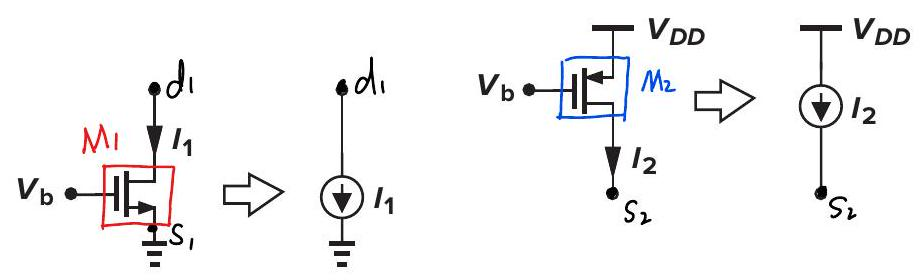
\includegraphics[max width=\textwidth, center]{2024_10_28_134d5d788a0919ac264dg-018(1)}

Figure 2.17 Saturated MOSFETs operating as current sources.

With $L$ assumed constant, a saturated MOSFET can be used as a current source connected between the drain and the source (Fig. 2.17), an important component in analog design. Note that the NMOS current source injects current into ground and the PMOS current source draws current from $V_{D D}$. In other words, only one terminal of each current source is "floating." (It is difficult to design a current source that flows between two arbitrary nodes of a circuit.)

\section*{Example 2.2}
On a $V_{D S}-V_{G S}$ plane, show the regions of operation of an NMOS transistor.\\
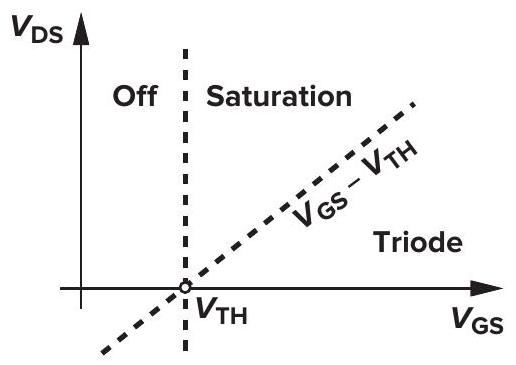
\includegraphics[max width=\textwidth, center]{2024_10_28_134d5d788a0919ac264dg-018}

Figure 2.18 $V_{D S}-V_{G S}$ plane showing regions of operation.

\section*{Solution}
Since the value of $V_{D S}$ with respect to $V_{G S}-V_{T H}$ determines the region of operation, we draw the line $V_{D S}=$ $V_{G S}-V_{T H}$ in the plane, as shown in Fig. 2.18. If $V_{G S}>V_{T H}$, then the region above the line corresponds to saturation, and that below the line corresponds to the triode region. Note that for a given $V_{D S}$, the device eventually leaves saturation as $V_{G S}$ increases. The minimum allowable $V_{D S}$ for operation in saturation is also called $V_{D, s a t}$. It is important to bear in mind that $V_{D, s a t}=V_{G S}-V_{T H}$.

The distinction between saturation and triode regions can be confusing, especially for PMOS devices. Intuitively, we note that the channel is pinched off if the difference between the gate and drain voltages is not sufficient to create an inversion layer. As depicted conceptually in Fig. 2.19, as $V_{G}-V_{D}$ of an NFET drops below $V_{T H}$, pinch-off occurs. Similarly, if $V_{D}-V_{G}$ of a PFET is not large enough ( $<\left|V_{T H P}\right|$ ), the device is saturated. Note that this view does not require knowledge of the source voltage. This means that we must know a priori which terminal operates as the drain. The drain is defined as the terminal with a higher (lower) voltage than the source for an NFET (PFET).\\
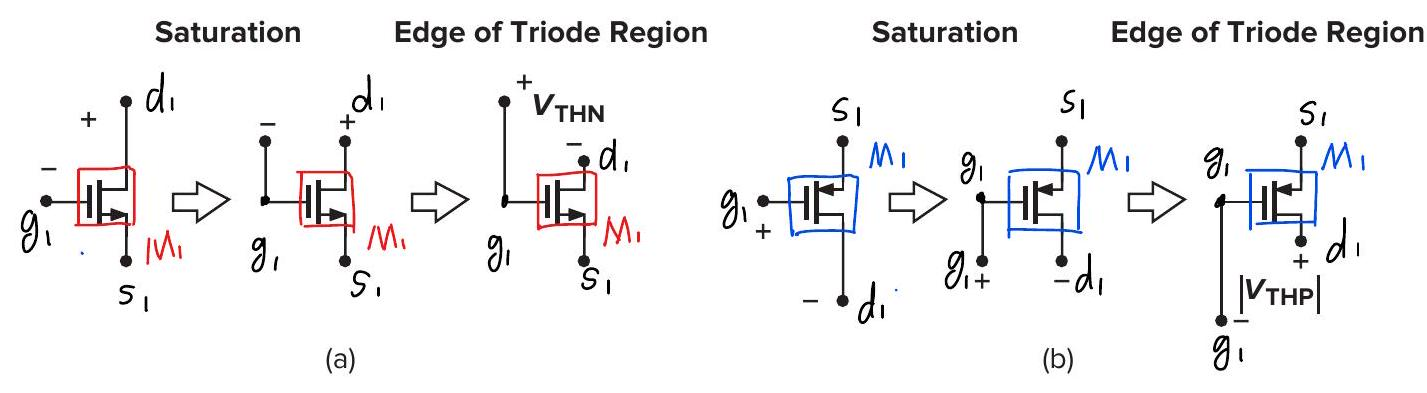
\includegraphics[max width=\textwidth, center]{2024_10_28_134d5d788a0919ac264dg-019(1)}

Figure 2.19 Conceptual visualization of saturation and triode regions.

\subsection*{2.2.3 MOS Transconductance}
Since a MOSFET operating in saturation produces a current in response to its gate-source overdrive voltage, we may define a figure of merit that indicates how well a device converts a voltage to a current. More specifically, since in processing signals, we deal with the changes in voltages and currents, we define the figure of merit as the change in the drain current divided by the change in the gate-source voltage. Called the "transconductance" (and usually defined in the saturation region) and denoted by $g_{m}$, this quantity is expressed as


\begin{align*}
g_{m} & =\left.\frac{\partial I_{D}}{\partial V_{G S}}\right|_{V D S \text { const. }}  \tag{2.17}\\
& =\mu_{n} C_{o x} \frac{W}{L}\left(V_{G S}-V_{T H}\right) \tag{2.18}
\end{align*}


In a sense, $g_{m}$ represents the sensitivity of the device: for a high $g_{m}$, a small change in $V_{G S}$ results in a large change in $I_{D}$. We express $g_{m}$ in $1 / \Omega$ or in siemens (S); e.g., $g_{m}=1 /(100 \Omega)=0.01 \mathrm{~S}$. In analog design, we sometimes say a MOSFET operates as a "transconductor" or a " $V / I$ converter" to indicate that it converts a voltage change to a current change. Interestingly, $g_{m}$ in the saturation region is equal to the inverse of $R_{o n}$ in the deep triode region.

The reader can prove that $g_{m}$ can also be expressed as


\begin{align*}
g_{m} & =\sqrt{2 \mu_{n} C_{o x} \frac{W}{L} I_{D}}  \tag{2.19}\\
& =\frac{2 I_{D}}{V_{G S}-V_{T H}} \tag{2.20}
\end{align*}


Plotted in Fig. 2.20, each of the above expressions proves useful in studying the behavior of $g_{m}$ as a function of one parameter while other parameters remain constant. For example, (2.18) suggests that\\
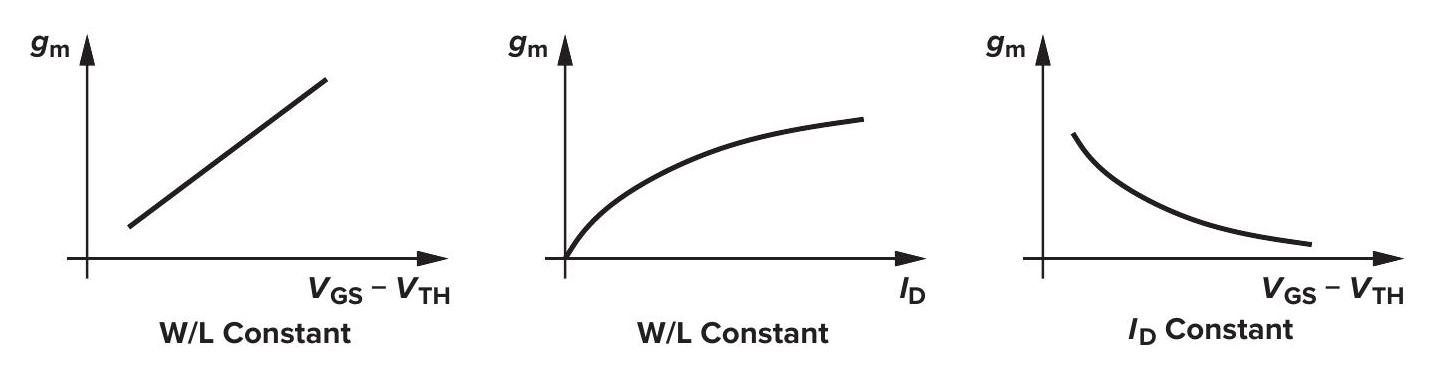
\includegraphics[max width=\textwidth, center]{2024_10_28_134d5d788a0919ac264dg-019}

Figure 2.20 Approximate MOS transconductance as a function of overdrive and drain current.\\
$g_{m}$ increases with the overdrive if $W / L$ is constant, whereas (2.20) implies that $g_{m}$ decreases with the overdrive if $I_{D}$ is constant.

The $I_{D}$ and $V_{G S}-V_{T H}$ terms in the above $g_{m}$ equations are bias values. For example, a transistor with $W / L=5 \mu \mathrm{~m} / 0.1 \mu \mathrm{~m}$ and biased at $I_{D}=0.5 \mathrm{~mA}$ may exhibit a transconductance of $(1 / 200 \Omega)$. If a signal is applied to the device, then $I_{D}$ and $V_{G S}-V_{T H}$ and hence $g_{m}$ vary, but in small-signal analysis, we assume that the signal amplitude is small enough that this variation is negligible.

Equation (2.19) implies that the transconductance can be raised arbitrarily if we increase $W / L$ and keep $I_{D}$ constant. This result is incorrect and will be revised in Sec. 2.3.

The concept of transconductance can also be applied to a device operating in the triode region, as illustrated in the following example.

\section*{Example 2.3}
For the arrangement shown in Fig. 2.21, plot the transconductance as a function of $V_{D S}$.\\
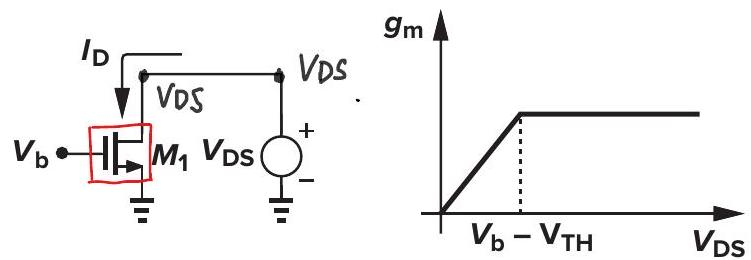
\includegraphics[max width=\textwidth, center]{2024_10_28_134d5d788a0919ac264dg-020}

Figure 2.21

\section*{Solution}
It is simpler to study $g_{m}$ as $V_{D S}$ decreases from infinity. So long as $V_{D S} \geq V_{b}-V_{T H}, M_{1}$ is in saturation, $I_{D}$ is relatively constant, and, from (2.19), so is $g_{m}$. If the drain voltage falls below the gate voltage by more than one threshold, $M_{1}$ enters the triode region, and


\begin{align*}
g_{m} & =\frac{\partial}{\partial V_{G S}}\left\{\frac{1}{2} \mu_{n} C_{o x} \frac{W}{L}\left[2\left(V_{G S}-V_{T H}\right) V_{D S}-V_{D S}^{2}\right]\right\}  \tag{2.21}\\
& =\mu_{n} C_{o x} \frac{W}{L} V_{D S} \tag{2.22}
\end{align*}


Thus, as plotted in Fig. 2.21, the transconductance drops in the triode region. For amplification, therefore, we usually employ MOSFETs in saturation.

For a PFET, the transconductance in the saturation region is expressed as $g_{m}=-\mu_{p} C_{o x}(W / L)$ $\left(V_{G S}-V_{T H}\right)=-2 I_{D} /\left(V_{G S}-V_{T H}\right)=\sqrt{2 \mu_{p} C_{o x}(W / L) I_{D}}$.

\section*{2.3 - Second-Order Effects}
Our analysis of the MOS structure has thus far entailed various simplifying assumptions, some of which are not valid in many analog circuits. In this section, we describe three second-order effects that are essential in our subsequent circuit analyses. Other phenomena that appear in nanometer devices are studied in Chapter 17.

Body Effect In the analysis of Fig. 2.10, we tacitly assumed that the bulk and the source of the transistor were tied to ground. What happens if the bulk voltage of an NFET drops below the source voltage (Fig. 2.22)? Since the S and D junctions remain reverse-biased, we surmise that the device continues to operate properly, but some of its characteristics may change. To understand the effect, suppose\\
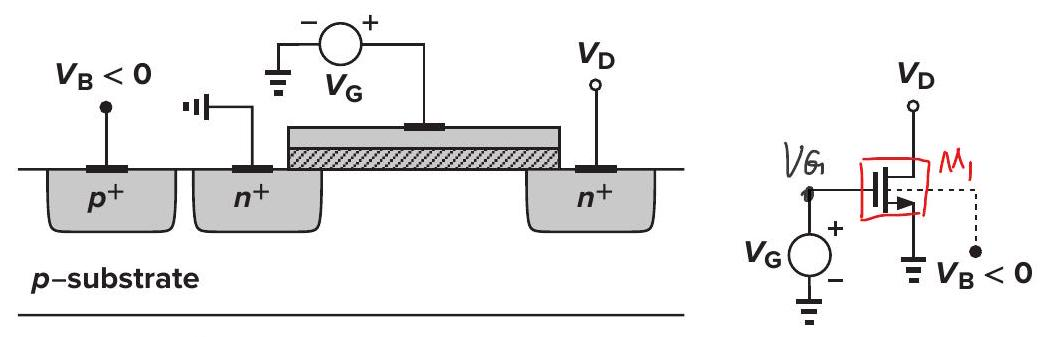
\includegraphics[max width=\textwidth, center]{2024_10_28_134d5d788a0919ac264dg-021(2)}

Figure 2.22 NMOS device with negative bulk voltage.\\
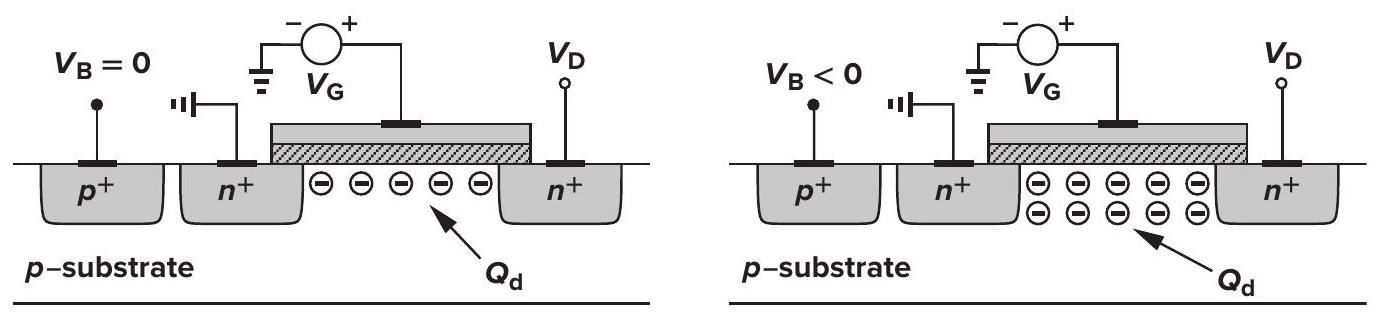
\includegraphics[max width=\textwidth, center]{2024_10_28_134d5d788a0919ac264dg-021(3)}

Figure 2.23 Variation of depletion region charge with bulk voltage.\\
$V_{S}=V_{D}=0$, and $V_{G}$ is somewhat less than $V_{T H}$, so that a depletion region is formed under the gate but no inversion layer exists. As $V_{B}$ becomes more negative, more holes are attracted to the substrate connection, leaving a larger negative charge behind; i.e., as depicted in Fig. 2.23, the depletion region becomes wider. Now recall from Eq. (2.1) that the threshold voltage is a function of the total charge in the depletion region because the gate charge must mirror $Q_{d}$ before an inversion layer is formed. Thus, as $V_{B}$ drops and $Q_{d}$ increases, $V_{T H}$ also increases. This phenomenon is called the "body effect" or the "back-gate effect."

It can be proved that with body effect,


\begin{equation*}
V_{T H}=V_{T H 0}+\gamma\left(\sqrt{2 \Phi_{F}+V_{S B}}-\sqrt{\left|2 \Phi_{F}\right|}\right) \tag{2.23}
\end{equation*}


where $V_{T H 0}$ is given by $(2.1), \gamma=\sqrt{2 q \epsilon_{s i} N_{s u b}} / C_{o x}$ denotes the body-effect coefficient, and $V_{S B}$ is the source-bulk potential difference [1]. The value of $\gamma$ typically lies in the range of 0.3 to $0.4 \mathrm{~V}^{1 / 2}$.

\section*{Example 2.4}
In Fig. 2.24(a), plot the drain current if $V_{X}$ varies from $-\infty$ to 0 . Assume $V_{T H 0}=0.3 \mathrm{~V}, \gamma=0.4 \mathrm{~V}^{1 / 2}$, and $2 \Phi_{F}=0.7 \mathrm{~V}$.\\
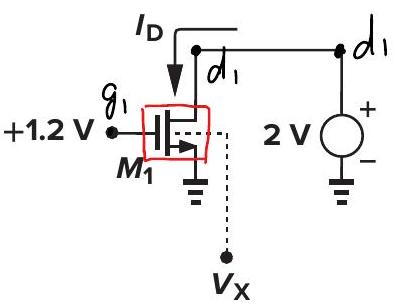
\includegraphics[max width=\textwidth, center]{2024_10_28_134d5d788a0919ac264dg-021}\\
(a)\\
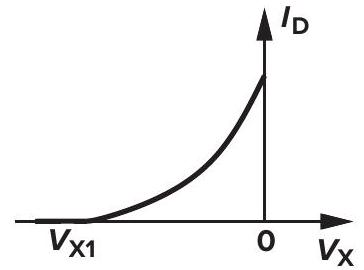
\includegraphics[max width=\textwidth, center]{2024_10_28_134d5d788a0919ac264dg-021(1)}\\
(b)

Figure 2.24

\section*{Solution}
If $V_{X}$ is sufficiently negative, the threshold voltage of $M_{1}$ exceeds 1.2 V and the device is off. That is,


\begin{equation*}
1.2 \mathrm{~V}=0.3+0.4\left(\sqrt{0.7-V_{X 1}}-\sqrt{0.7}\right) \tag{2.24}
\end{equation*}


and hence $V_{X 1}=-8.83 \mathrm{~V}$. For $V_{X 1}<V_{X}<0, I_{D}$ increases according to


\begin{equation*}
I_{D}=\frac{1}{2} \mu_{n} C_{o x} \frac{W}{L}\left[V_{G S}-V_{T H 0}-\gamma\left(\sqrt{2 \Phi_{F}-V_{X}}-\sqrt{2 \Phi_{F}}\right)\right]^{2} \tag{2.25}
\end{equation*}


Fig. 2.24(b) shows the resulting behavior.

For body effect to manifest itself, the bulk potential, $V_{\text {sub }}$, need not change: if the source voltage varies with respect to $V_{\text {sub }}$, the same phenomenon occurs. For example, consider the circuit in Fig. 2.25(a), first ignoring body effect. We note that as $V_{\text {in }}$ varies, $V_{\text {out }}$ closely follows the input because the drain current remains equal to $I_{1}$. In fact, we can write


\begin{equation*}
I_{1}=\frac{1}{2} \mu_{n} C_{o x} \frac{W}{L}\left(V_{\text {in }}-V_{\text {out }}-V_{T H}\right)^{2} \tag{2.26}
\end{equation*}


concluding that $V_{\text {in }}-V_{\text {out }}$ is constant if $I_{1}$ is constant [Fig. 2.25(b)].\\
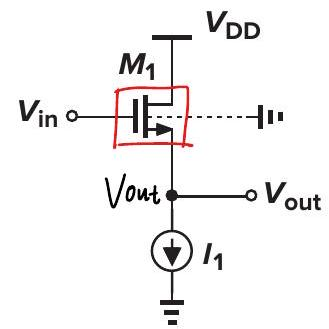
\includegraphics[max width=\textwidth, center]{2024_10_28_134d5d788a0919ac264dg-022}\\
(a)\\
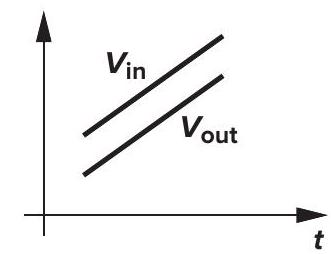
\includegraphics[max width=\textwidth, center]{2024_10_28_134d5d788a0919ac264dg-022(2)}\\
(b)\\
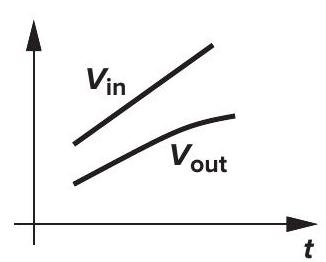
\includegraphics[max width=\textwidth, center]{2024_10_28_134d5d788a0919ac264dg-022(1)}\\
(c)

Figure 2.25 (a) A circuit in which the source-bulk voltage varies with input level; (b) input and output voltages with no body effect; (c) input and output voltages with body effect.

Now suppose that the substrate is tied to ground and body effect is significant. Then, as $V_{i n}$ and hence $V_{\text {out }}$ become more positive, the potential difference between the source and the bulk increases, raising the value of $V_{T H}$. Equation (2.26) implies that $V_{i n}-V_{\text {out }}$ must increase so as to maintain $I_{D}$ constant [Fig. 2.25(c)].

Body effect is usually undesirable. The change in the threshold voltage, e.g., as in Fig. 2.25(a), often complicates the design of analog (and even digital) circuits. Device technologists balance $N_{s u b}$ and $C_{o x}$ to obtain a reasonable value for $\gamma$.

\section*{Example 2.5}
Equation (2.23) suggests that if $V_{S B}$ becomes negative, then $V_{T H}$ decreases. Is this correct?

\section*{Solution}
Yes, it is. If the bulk voltage of an NMOS device rises above its source voltage, $V_{T H}$ falls below $V_{T H 0}$. This observation proves useful in low-voltage design, where the performance of a circuit may suffer due to a high threshold voltage; one can bias the bulk to reduce $V_{T H}$. Unfortunately, this is not straightforward for NFETs because they typically share one substrate, but it can readily be applied to individual PFETs.

Channel-Length Modulation In the analysis of channel pinch-off in Sec. 2.2, we noted that the actual length of the channel gradually decreases as the potential difference between the gate and the drain decreases. In other words, in (2.13), $L^{\prime}$ is in fact a function of $V_{D S}$. This effect is called "channel-length modulation." Writing $L^{\prime}=L-\Delta L$, i.e., $1 / L^{\prime} \approx(1+\Delta L / L) / L$, and assuming a first-order relationship between $\Delta L / L$ and $V_{D S}$, such as $\Delta L / L=\lambda V_{D S}$, we have, in saturation,


\begin{equation*}
I_{D} \approx \frac{1}{2} \mu_{n} C_{o x} \frac{W}{L}\left(V_{G S}-V_{T H}\right)^{2}\left(1+\lambda V_{D S}\right) \tag{2.27}
\end{equation*}


where $\lambda$ is the "channel-length modulation coefficient." Illustrated in Fig. 2.26, this phenomenon results in a nonzero slope in the $I_{D} / V_{D S}$ characteristic and hence a nonideal current source between D and S in saturation. The parameter $\lambda$ represents the relative variation in length for a given increment in $V_{D S}$. Thus, for longer channels, $\lambda$ is smaller.\\
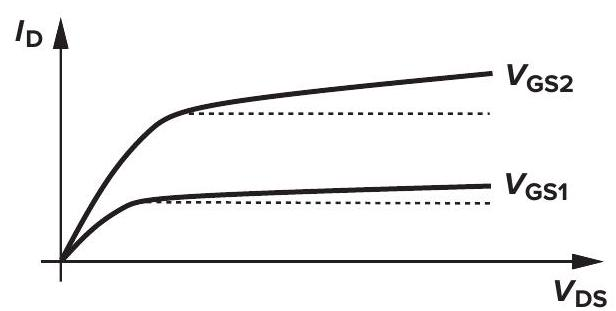
\includegraphics[max width=\textwidth, center]{2024_10_28_134d5d788a0919ac264dg-023(1)}

Figure 2.26 Finite saturation region slope resulting from channel-length modulation.

\section*{Example 2.6}
Is there channel-length modulation in the triode region?

\section*{Solution}
No, there is not. In the triode region, the channel continuously stretches from the source to the drain, experiencing no pinch-off. Thus, the drain voltage does not modulate the length of the channel.

The reader may then observe a discontinuity in the equations as the device goes from the triode region to saturation:


\begin{align*}
I_{D, t r i} & =\frac{1}{2} \mu_{n} C_{o x} \frac{W}{L}\left[2\left(V_{G S}-V_{T H}\right) V_{D S}-V_{D S}^{2}\right]  \tag{2.28}\\
I_{D, s a t} & =\frac{1}{2} \mu_{n} C_{o x} \frac{W}{L}\left(V_{G S}-V_{T H}\right)^{2}\left(1+\lambda V_{D S}\right) \tag{2.29}
\end{align*}


The former yields $(1 / 2) \mu_{n} C_{o x} W / L\left(V_{G S}-V_{T H}\right)^{2}$ at the edge of the triode region, whereas the latter exhibits an additional factor of $1+\lambda V_{D S}$. This discrepancy is removed in more complex models of MOSFETs (Chapter 17).

With channel-length modulation, some of the expressions derived for $g_{m}$ must be modified. Equations (2.18) and (2.19) are respectively rewritten as


\begin{align*}
g_{m} & =\mu_{n} C_{o x} \frac{W}{L}\left(V_{G S}-V_{T H}\right)\left(1+\lambda V_{D S}\right)  \tag{2.30}\\
& =\sqrt{2 \mu_{n} C_{o x}(W / L) I_{D}\left(1+\lambda V_{D S}\right)} \tag{2.31}
\end{align*}


while Eq. (2.20) remains unchanged.

\section*{Nanometer Design Notes}
Nanometer transistors suffer from various imperfections and markedly depart from square-law behavior. Shown below are the actual I-V characteristics of an NFET with $W / L=5 \mu \mathrm{~m} / 40 \mathrm{~nm}$ for $V_{G S}=0.3 \mathrm{~V} \cdots 0.8 \mathrm{~V}$. Also plotted are the characteristics of a square-law device of the same dimensions. Despite our best efforts to match the latter device to the former, we still observe significant differences.\\
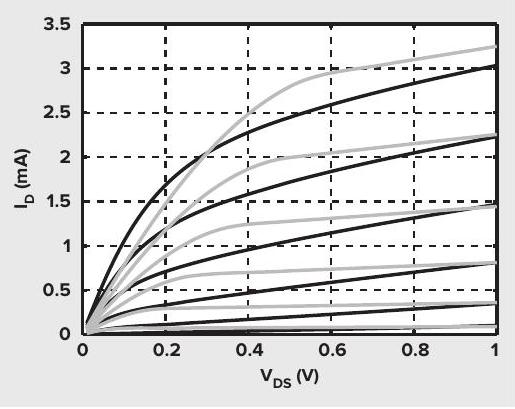
\includegraphics[max width=\textwidth, center]{2024_10_28_134d5d788a0919ac264dg-023}

Example 2.7\\
Keeping all other parameters constant, plot the $I_{D} / V_{D S}$ characteristic of a MOSFET for $L=L_{1}$ and $L=2 L_{1}$.

\section*{Solution}
Writing


\begin{equation*}
I_{D}=\frac{1}{2} \mu_{n} C_{o x} \frac{W}{L}\left(V_{G S}-V_{T H}\right)^{2}\left(1+\lambda V_{D S}\right) \tag{2.32}
\end{equation*}


and $\lambda \propto 1 / L$, we note that if the length is doubled, the slope of $I_{D}$ vs. $V_{D S}$ is divided by four because $\partial I_{D} / \partial V_{D S} \propto$ $\lambda / L \propto 1 / L^{2}$ (Fig. 2.27). (This is true only if $V_{G S}-V_{T H}$ is constant.) For a given gate-source overdrive, a larger $L$ gives a more ideal current source while degrading the current capability of the device. Thus, $W$ may need to be increased proportionally. In fact, if we double $W$ to restore $I_{D}$ to its original value, the slope also doubles. In other words, for a required drain current and a given overdrive, doubling the length reduces the slope by a factor of 2 .\\
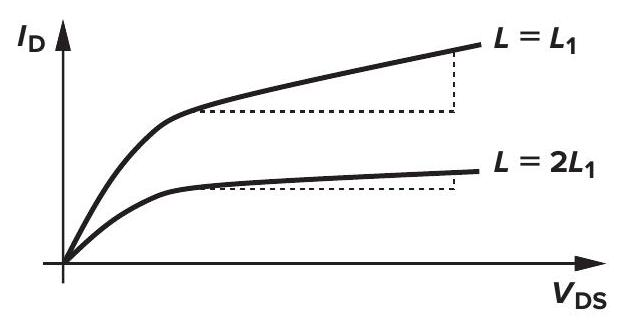
\includegraphics[max width=\textwidth, center]{2024_10_28_134d5d788a0919ac264dg-024}

Figure 2.27 Effect of doubling channel length.

The linear approximation $\Delta L / L \propto V_{D S}$ becomes less accurate in short-channel transistors, resulting in a variable slope in the saturated $I_{D} / V_{D S}$ characteristics. We return to this issue in Chapter 17.

The dependence of $I_{D}$ upon $V_{D S}$ in saturation may suggest that the bias current of a MOSFET can be defined by the proper choice of the drain-source voltage, allowing freedom in the choice of $V_{G S}-V_{T H}$. However, since the dependence on $V_{D S}$ is much weaker, the drain-source voltage is not used to set the current. That is, we always consider $V_{G S}-V_{T H}$ as the current-defining parameter. The effect of $V_{D S}$ on $I_{D}$ is usually considered an error, and it is studied in Chapter 5.

Subthreshold Conduction In our analysis of the MOSFET, we have assumed that the device turns off abruptly as $V_{G S}$ drops below $V_{T H}$. In reality, for $V_{G S} \approx V_{T H}$, a "weak" inversion layer still exists and some current flows from D to S . Even for $V_{G S}<V_{T H}, I_{D}$ is finite, but it exhibits an exponential dependence on $V_{G S}[2,3]$. Called "subthreshold conduction," this effect can be formulated for $V_{D S}$ greater than roughly 100 mV as


\begin{equation*}
I_{D}=I_{0} \exp \frac{V_{G S}}{\xi V_{T}} \tag{2.33}
\end{equation*}


where $I_{0}$ is proportional to $W / L, \xi>1$ is a nonideality factor, and $V_{T}=k T / q$. We also say the device operates in "weak inversion." (Similarly, for $V_{G S}>V_{T H}$, we say the device operates in "strong inversion.") Except for $\xi,(2.33)$ is similar to the exponential $I_{C} / V_{B E}$ relationship of a bipolar transistor. The key point here is that as $V_{G S}$ falls below $V_{T H}$, the drain current drops at a finite rate. With typical values of $\xi$, at room temperature $V_{G S}$ must decrease by approximately 80 mV for $I_{D}$ to decrease by one decade (Fig. 2.28). For example, if a threshold of 0.3 V is chosen in a process to allow low-voltage operation, then when $V_{G S}$ is reduced to zero, the drain current decreases by only a factor of $10^{0.3 \mathrm{~V} / 80 \mathrm{mV}}=10^{3.75} \approx 5.62 \times 10^{3}$. For example, if the transistor carries about $1 \mu \mathrm{~A}$ for $V_{G S}=V_{T H}$ and we have 100 million such devices, then\\
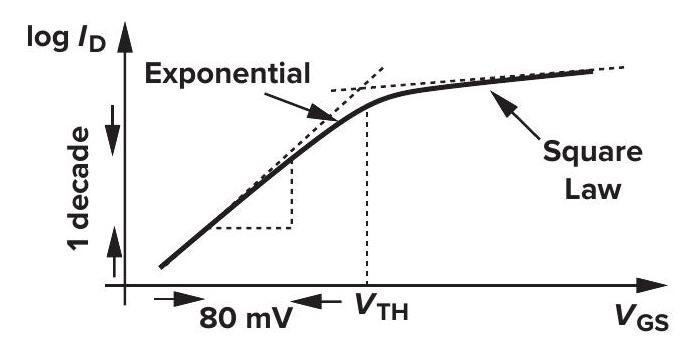
\includegraphics[max width=\textwidth, center]{2024_10_28_134d5d788a0919ac264dg-025}

Figure 2.28 MOS subthreshold characteristics.\\
they draw 18 mA when they are nominally off. Especially problematic in large circuits such as memories, subthreshold conduction can result in significant power dissipation (or loss of analog information).

If a MOS device conducts for $V_{G S}<V_{T H}$, then how do we define the threshold voltage? Indeed, numerous definitions have been proposed. One possibility is to extrapolate, on a logarithmic vertical scale, the weak inversion and strong inversion characteristics and consider their intercept voltage as the threshold (Fig. 2.28).

We now reexamine Eq. (2.19) for the transconductance of a MOS device operating in the subthreshold region. Is it possible to achieve an arbitrarily high transconductance by increasing $W$ while maintaining $I_{D}$ constant? Is it possible to obtain a higher transconductance than that of a bipolar transistor $\left(I_{C} / V_{T}\right)$ biased at the same current? Equation (2.19) was derived from the square-law characteristic $I_{D}=$ $(1 / 2) \mu_{n} C_{o x}(W / L)\left(V_{G S}-V_{T H}\right)^{2}$. However, if $W$ increases while $I_{D}$ remains constant, then $V_{G S} \rightarrow V_{T H}$ and the device enters the subthreshold region. As a result, the transconductance is calculated from (2.33) to be $g_{m}=I_{D} /\left(\xi V_{T}\right)$, revealing that MOSFETs are still inferior to bipolar transistors in this respect.

At what overdrive voltage can we say the transistor goes from strong inversion to weak inversion? While somewhat arbitrary, this transition point can be defined as the overdrive voltage, $\left(V_{G S}-V_{T H}\right)_{1}$, at which the corresponding transconductances would become equal for the same drain current:


\begin{equation*}
\frac{I_{D}}{\xi V_{T}}=\frac{2 I_{D}}{\left(V_{G S}-V_{T H}\right)_{1}} \tag{2.34}
\end{equation*}


and hence


\begin{equation*}
\left(V_{G S}-V_{T H}\right)_{1}=2 \xi V_{T} \tag{2.35}
\end{equation*}


For $\xi \approx 1.5$, this amounts to about 80 mV .\\
The exponential dependence of $I_{D}$ upon $V_{G S}$ in subthreshold operation may suggest the use of MOS devices in this regime so as to achieve a higher gain. However, since such conditions are met only by a large device width or low drain current, the speed of subthreshold circuits is severely limited.

\section*{Example 2.8}
Examine the behavior of a MOSFET as the drain "current density," $I_{D} / W$, varies.

\section*{Solution}
For a given drain current and device width, how do we determine the region of operation? We must consider the equations for both strong and weak inversion:


\begin{align*}
I_{D} & =\frac{1}{2} \mu_{n} C_{o x} \frac{W}{L}\left(V_{G S}-V_{T H}\right)^{2}  \tag{2.36}\\
I_{D} & =\alpha \frac{W}{L} \exp \frac{V_{G S}}{\xi V_{T}} \tag{2.37}
\end{align*}


where channel-length modulation is neglected and $I_{0}$ in Eq. (2.33) has been expressed as a proportionality factor, $\alpha$, multiplied by $W / L$. What happens if the device is in strong inversion and we continue to reduce $I_{D}$ while $W / L$ is constant? Can $V_{G S}$ simply approach $V_{T H}$ to yield an arbitrarily small value for $\left(V_{G S}-V_{T H}\right)^{2}$ ? Why does the square-law equation not hold as $V_{G S}$ approaches $V_{T H}$ ?

To answer these questions, we return to the plot of Fig. 2.28 and observe that only currents beyond a certain level can be supported in strong inversion. In other words, for a given current and $W / L$, we must obtain $V_{G S}$ from both the square-law and exponential equations and select the lower value:


\begin{align*}
V_{G S} & =\sqrt{\frac{2 I_{D}}{\mu_{n} C_{o x} W / L}}+V_{T H}  \tag{2.38}\\
V_{G S} & =\xi V_{T} \ln \frac{I_{D}}{\alpha W / L} \tag{2.39}
\end{align*}


If $I_{D}$ remains constant and $W$ increases, $V_{G S}$ falls and the device goes from strong inversion to weak inversion.

Voltage Limitations A MOSFET experiences various undesirable effects if its terminal voltage differences exceed certain limits (if the device is "stressed"). At high gate-source voltages, the gate oxide breaks down irreversibly, damaging the transistor. In short-channel devices, an excessively large drain-source voltage widens the depletion region around the drain so much that it touches that around the source, creating a very large drain current. (This effect is called "punchthrough.") Even without breakdown, MOSFETs' characteristics can change permanently if the terminal voltage differences exceed a specified value. Such effects are described in Chapter 17.

\section*{2.4 ■ MOS Device Models}
\subsection*{2.4.1 MOS Device Layout}
For the developments in subsequent sections, it is beneficial to have some understanding of the layout of a MOSFET. We describe only a simple view here, deferring the fabrication details and structural subtleties to Chapters 18 and 19.

The layout of a MOSFET is determined by both the electrical properties required of the device in the circuit and the "design rules" imposed by the technology. For example, $W / L$ is chosen to set the transconductance or other circuit parameters while the minimum $L$ is dictated by the process. In addition to the gate, the source and drain areas must be defined properly as well.

Shown in Fig. 2.29 are the "bird's-eye view" and the top view of a MOSFET. The gate polysilicon and the source and drain terminals must be tied to metal (aluminum) wires that serve as interconnects with low resistance and capacitance. To accomplish this, one or more "contact windows" must be opened in each region, filled with metal, and connected to the upper metal wires. Note that the gate poly extends beyond the channel area by some amount to ensure reliable definition of the "edge" of the transistor.

The source and drain junctions play an important role in the performance. To minimize the capacitance of $S$ and $D$, the total area of each junction must be minimized. We see from Fig. 2.29 that one dimension of the junctions is equal to $W$. The other dimension must be large enough to accommodate the contact windows and is specified by the technology design rules. ${ }^{7}$

\footnotetext{${ }^{7}$ This dimension is typically three to four times the minimum allowable channel length.
}
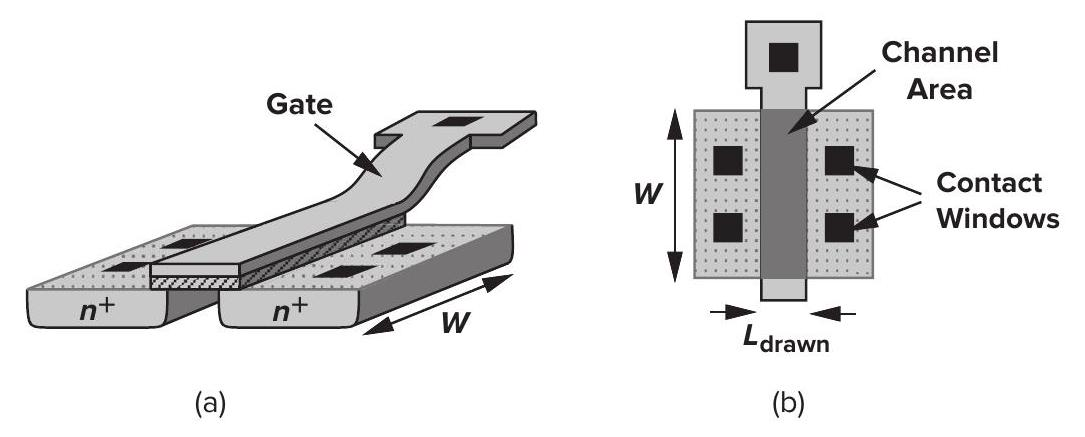
\includegraphics[max width=\textwidth, center]{2024_10_28_134d5d788a0919ac264dg-027}

Figure 2.29 Bird's-eye and vertical views of a MOS device.

\section*{Example 2.9}
Draw the layout of the circuit shown in Fig. 2.30(a).\\
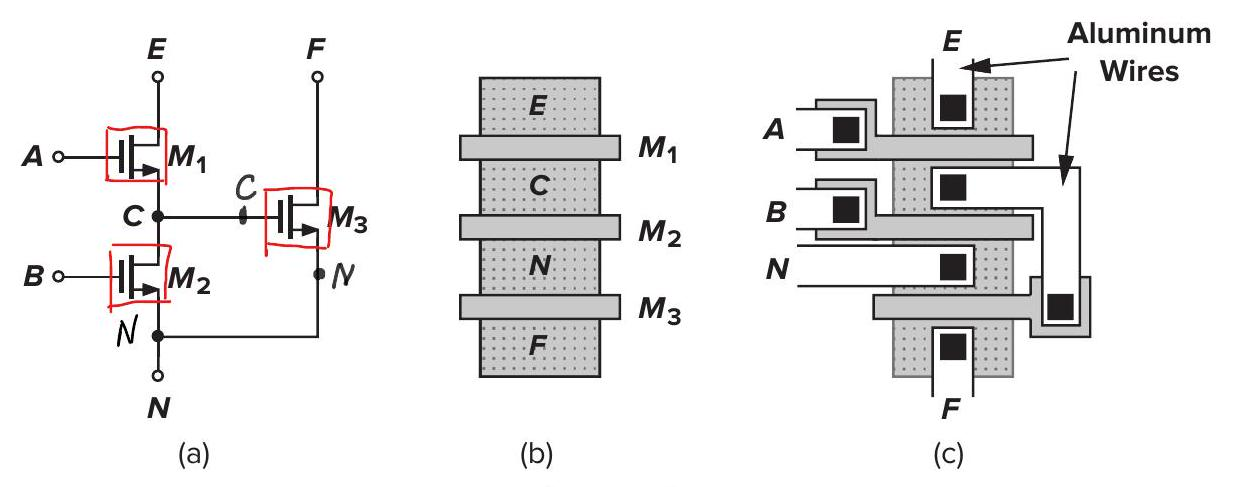
\includegraphics[max width=\textwidth, center]{2024_10_28_134d5d788a0919ac264dg-027(1)}

Figure 2.30

\section*{Solution}
Observing that $M_{1}$ and $M_{2}$ share the same $\mathrm{S} / \mathrm{D}$ junctions at node $C$ and $M_{2}$ and $M_{3}$ also do so at node $N$, we surmise that the three transistors can be laid out as shown in Fig. 2.30(b). Connecting the remaining terminals, we obtain the layout in Fig. 2.30(c). Note that the gate polysilicon of $M_{3}$ cannot be directly tied to the source material of $M_{1}$, thus requiring a metal interconnect.

\subsection*{2.4.2 MOS Device Capacitances}
The basic quadratic I/V relationships derived in the previous section, along with corrections for body effect and channel-length modulation, provide some understanding of the low-frequency behavior of CMOS circuits. In many analog circuits, however, the capacitances associated with the devices must also be taken into account so as to predict the high-frequency behavior as well.

We expect that a capacitance exists between every two of the four terminals of a MOSFET (Fig. 2.31). ${ }^{8}$ Moreover, the value of each of these capacitances may depend on the bias conditions of the transistor.

\footnotetext{${ }^{8}$ The capacitance between $S$ and $D$ is negligible.
}
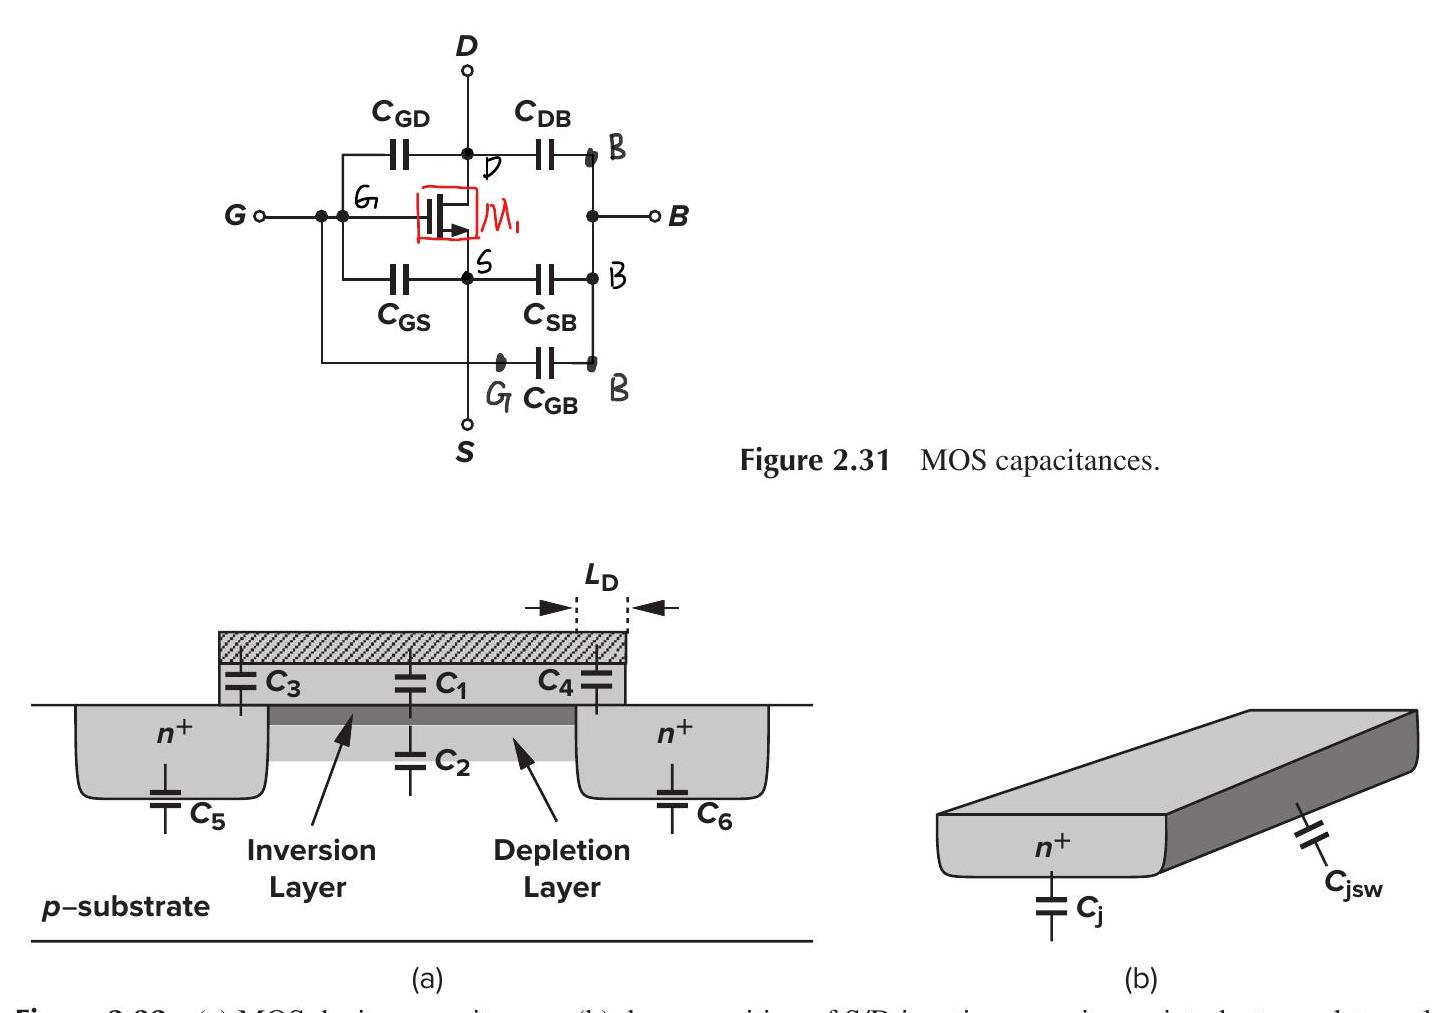
\includegraphics[max width=\textwidth, center]{2024_10_28_134d5d788a0919ac264dg-028(1)}

Figure 2.32 (a) MOS device capacitances; (b) decomposition of S/D junction capacitance into bottom-plate and sidewall components.

\section*{Nanometer Design Notes}
New generations of CMOS technology incorporate the "FinFET" structure. Unlike the conventional "planar" device, the FinFET extends in the third dimension. As shown below, it consists of an $n^{+}$ wall (resembling a shark's fin) and a gate that wraps around the wall. The transistor carries current from the source to the drain on the surfaces of the fin. Owing to the tight confinement of the electric field between the two vertical walls of the gate, the FinFET exhibits less channel-length modulation and subthreshold leakage. But where do the S/D contacts land? What other issues do we face in FinFETs? We return to these questions later in this book.\\
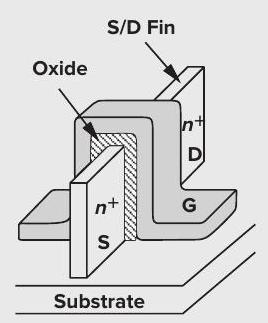
\includegraphics[max width=\textwidth, center]{2024_10_28_134d5d788a0919ac264dg-028}

Considering the physical structure in Fig. 2.32(a), we identify the following: (1) the oxide capacitance between the gate and the channel, $C_{1}=W L C_{o x}$; (2) the depletion capacitance between the channel and the substrate, $C_{2}=$ $W L \sqrt{q \epsilon_{s i} N_{s u b} /\left(4 \Phi_{F}\right)}$; and (3) the capacitance due to the overlap of the gate poly with the source and drain areas, $C_{3}$ and $C_{4}$. Owing to fringing electric field lines, $C_{3}$ and $C_{4}$ cannot be simply written as $W L_{D} C_{o x}$, and are usually obtained by more elaborate calculations. The overlap capacitance per unit width is denoted by $C_{o v}$ and expressed in $\mathrm{F} / \mathrm{m}$ (or $\mathrm{fF} / \mu \mathrm{m}$ ). We simply multiply $C_{o v}$ by $W$ to find the gate-source and gate-drain overlap capacitances. (4) The junction capacitance between the source/drain areas and the substrate. As shown in Fig. 2.32(b), this last capacitance is decomposed into two components: the bottom-plate capacitance associated with the bottom of the junction, $C_{j}$, and the sidewall capacitance due to the perimeter of the junction, $C_{j s w}$. The distinction is necessary because different transistor geometries yield different area and perimeter values for the S/D junctions. We specify $C_{j}$ and $C_{j s w}$ as capacitance per unit area (in $\mathrm{F} / \mathrm{m}^{2}$ ) and unit length (in $\mathrm{F} / \mathrm{m}$ ), respectively. Thus, $C_{j}$ is multiplied by the S/D area, and $C_{j s w}$ by the S/D perimeter. Note that each junction capacitance can be expressed as $C_{j}=C_{j 0} /\left[1+V_{R} /\left(\Phi_{B}\right)\right]^{m}$, where $V_{R}$ is the reverse voltage across the junction, $\Phi_{B}$ is the junction built-in potential, and $m$ is a power typically in the range of 0.3 and 0.4 .

\section*{Example 2.10}
Calculate the source and drain junction capacitances of the two structures shown in Fig. 2.33.\\
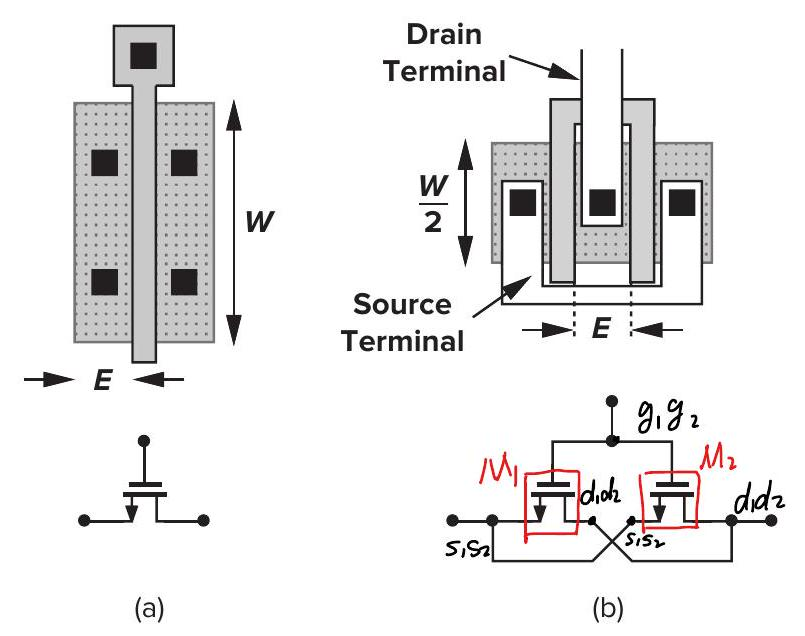
\includegraphics[max width=\textwidth, center]{2024_10_28_134d5d788a0919ac264dg-029}

Figure 2.33

\section*{Solution}
For the transistor in Fig. 2.33(a), we have


\begin{equation*}
C_{D B}=C_{S B}=W E C_{j}+2(W+E) C_{j s w} \tag{2.40}
\end{equation*}


whereas for that in Fig. 2.33(b),


\begin{align*}
C_{D B} & =\frac{W}{2} E C_{j}+2\left(\frac{W}{2}+E\right) C_{j s w}  \tag{2.41}\\
C_{S B} & =2\left[\frac{W}{2} E C_{j}+2\left(\frac{W}{2}+E\right) C_{j s w}\right]  \tag{2.42}\\
& =W E C_{j}+2(W+2 E) C_{j s w} \tag{2.43}
\end{align*}


Called a "folded" structure, the geometry in Fig. 2.33(b) exhibits substantially less drain junction capacitance than that in Fig. 2.33(a) while providing the same $W / L$.

In the above calculations, we have assumed that the total source or drain perimeter, $2(W+E)$, is multiplied by $C_{j s w}$. In reality, the capacitance of the inner sidewall (under the gate) may be different from that of the other sidewalls. ${ }^{9}$ Nonetheless, we typically assume that all four sides have the same $C_{j s w}$. The error resulting from this assumption is negligible because each node in a circuit is connected to a number of other device capacitances as well.

We now derive the capacitances between terminals of a MOSFET in different regions of operation. If the device is off, $C_{G D}=C_{G S}=C_{o v} W$, and the gate-bulk capacitance consists of the series combination of the gate-oxide capacitance and the depletion-region capacitance [Fig. 2.32(a)], i.e., $C_{G B}=\left(W L C_{o x}\right) C_{d} /\left(W L C_{o x}+C_{d}\right)$, where $L$ is the effective length, $C_{d}=W L \sqrt{q \epsilon_{s i} N_{s u b} /\left(4 \Phi_{F}\right)}$, and

\footnotetext{${ }^{9}$ This is because the other sidewalls are surrounded by a "trench" (Chapter 18).
}
$\epsilon_{s i}=\epsilon_{r, s i} \times \epsilon_{0}=11.8 \times\left(8.85 \times 10^{-14}\right) \mathrm{F} / \mathrm{cm}$. The value of $C_{S B}$ and $C_{D B}$ is a function of the source and drain voltages with respect to the substrate.

If the device is in the deep triode region, i.e., if $S$ and $D$ have approximately equal voltages, then the gate-channel capacitance, $W L C_{o x}$, is divided equally between the gate and source terminals and the gate and drain terminals (Fig. 2.34). This is because a change of $\Delta V$ in the gate voltage draws equal amounts of charge from S and D . Thus, $C_{G D}=C_{G S}=W L C_{o x} / 2+W C_{o v}$.\\
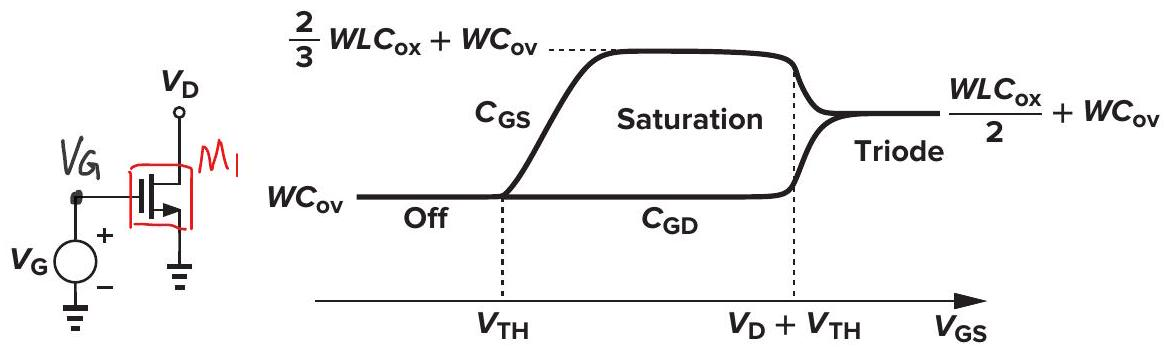
\includegraphics[max width=\textwidth, center]{2024_10_28_134d5d788a0919ac264dg-030(1)}

Figure 2.34 Variation of gate-source and gate-drain capacitances versus $V_{G S}$.

Let us now consider $C_{G D}$ and $C_{G S}$. If in saturation, a MOSFET exhibits a gate-drain capacitance roughly equal to $W C_{o v}$. As for $C_{G S}$, we note that the potential difference between the gate and the channel varies from $V_{G S}$ at the source to $V_{T H}$ at the pinch-off point, resulting in a nonuniform vertical electric field in the gate oxide as we travel from the source to the drain. It can be proved that the equivalent capacitance of this structure, excluding the gate-source overlap capacitance, equals (2/3)WLC $C_{o x}$ [1]. Thus, $C_{G S}=2 W L_{e f f} C_{o x} / 3+W C_{o v}$. The behavior of $C_{G D}$ and $C_{G S}$ in different regions of operation is plotted in Fig. 2.34. Note that the above equations do not provide a smooth transition from one region of operation to another, creating convergence difficulties in simulation programs. This issue is revisited in Chapter 17.

The gate-bulk capacitance is usually neglected in the triode and saturation regions because the inversion layer acts as a "shield" between the gate and the bulk. In other words, if the gate voltage varies, the charge is supplied by the source and the drain rather than the bulk.

Example 2.11\\
Sketch the capacitances of $M_{1}$ in Fig. 2.35 as $V_{X}$ varies from zero to 3 V . Assume that $V_{T H}=0.3 \mathrm{~V}$ and $\lambda=\gamma=0$.\\
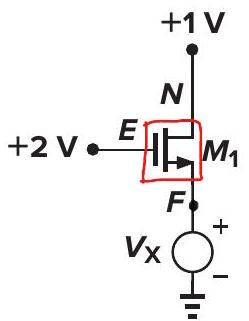
\includegraphics[max width=\textwidth, center]{2024_10_28_134d5d788a0919ac264dg-030}

Figure 2.35

\section*{Solution}
To avoid confusion, we label the three terminals as shown in Fig. 2.35 and denote the bulk by $B$. For $V_{X} \approx 0, M_{1}$ is in the triode region, $C_{E N} \approx C_{E F}=(1 / 2) W L C_{o x}+W C_{o v}$, and $C_{F B}$ is maximum. The value of $C_{N B}$ is independent of $V_{X}$. As $V_{X}$ exceeds 1 V , the role of the source and drain is exchanged [Fig. 2.36(a)], eventually bringing $M_{1}$ out of the triode region for $V_{X} \geq 2 \mathrm{~V}-0.3 \mathrm{~V}$. The variation of the capacitances is plotted in Figs. 2.36(b) and (c).\\
\includegraphics[max width=\textwidth, center]{2024_10_28_134d5d788a0919ac264dg-031}

Figure 2.36

\subsection*{2.4.3 MOS Small-Signal Model}
The quadratic characteristics described by (2.8) and (2.9) along with the voltage-dependent capacitances derived above form the large-signal model of MOSFETs. Such a model proves essential in analyzing circuits in which the signal significantly disturbs the bias points, particularly if nonlinear effects are of concern. By contrast, if the perturbation in bias conditions is small, a "small-signal" model, i.e., an approximation of the large-signal model around the operating point, can be employed to simplify the calculations. Since in many analog circuits, MOSFETs are biased in the saturation region, we derive the corresponding small-signal model here. For transistors operating as switches, a linear resistor given by (2.11) together with device capacitances serves as a rough small-signal equivalent.

We derive the small-signal model by producing a small increment in one bias parameter and calculating the resulting increment in other bias parameters. Specifically, we (1) apply certain bias voltages to the terminals of the device, (2) increment the potential difference between two of the terminals while other terminal voltages remain constant, and (3) measure the resulting change in all terminal currents. If we change the voltage between two terminals by $\Delta V$ and measure a current change of $\Delta I$ in some branch, we can model the effect by a voltage-dependent current source. Let us apply a change to the gate-source voltage, $\Delta V=V_{G S}$, where $V_{G S}$ is a small-signal quantity. ${ }^{10}$ The drain current therefore changes by $g_{m} V_{G S}$ and is modeled by a voltage-dependent current source tied between the drain and source terminals [Fig. 2.37(a)]. The gate current is very small and its change is negligible, thus requiring no representation here. The result is the small-signal model of an ideal MOSFET-the model that an analog designer applies to most devices in a circuit at first glance.

Owing to channel-length modulation, the drain current also varies with the drain-source voltage. This effect can be modeled by a voltage-dependent current source [Fig. 2.37(b)], but a current source whose value linearly depends on the voltage across it is equivalent to a linear resistor [Fig. 2.37(c)] (why?). Tied between D and S , the resistor is given by


\begin{align*}
r_{O} & =\frac{\partial V_{D S}}{\partial I_{D}}  \tag{2.44}\\
& =\frac{1}{\partial I_{D} / \partial V_{D S}}  \tag{2.45}\\
& =\frac{1}{\frac{1}{2} \mu_{n} C_{o x} \frac{W}{L}\left(V_{G S}-V_{T H}\right)^{2} \cdot \lambda} \tag{2.46}
\end{align*}


\footnotetext{${ }^{10}$ In this book, we use uppercase letters to denote large-signal or small-signal quantities. The distinction will be clear from the context.
}
\includegraphics[max width=\textwidth, center]{2024_10_28_134d5d788a0919ac264dg-032}

Figure 2.37 (a) Basic MOS small-signal model; (b) channel-length modulation represented by a dependent current source; (c) channel-length modulation represented by a resistor; (d) body effect represented by a dependent current source.


\begin{align*}
& \approx \frac{1+\lambda V_{D S}}{\lambda I_{D}}  \tag{2.47}\\
& \approx \frac{1}{\lambda I_{D}} \tag{2.48}
\end{align*}


where it is assumed that $\lambda V_{D S} \ll 1$. As seen throughout this book, the output resistance, $r_{O}$, affects the performance of many analog circuits. For example, $r_{O}$ limits the maximum voltage gain of most amplifiers.

Now recall that the bulk potential influences the threshold voltage and hence the gate-source overdrive. As demonstrated in Example 2.3, with all other terminals held at a constant voltage, the drain current is a function of the bulk voltage. That is, the bulk behaves as a second gate. Modeling this dependence by a current source connected between D and S [Fig. 2.37(d)], we write the value as $g_{m b} V_{b s}$, where $g_{m b}=\partial I_{D} / \partial V_{B S}$. In the saturation region, $g_{m b}$ can be expressed as


\begin{align*}
g_{m b} & =\frac{\partial I_{D}}{\partial V_{B S}}  \tag{2.49}\\
& =\mu_{n} C_{o x} \frac{W}{L}\left(V_{G S}-V_{T H}\right)\left(-\frac{\partial V_{T H}}{\partial V_{B S}}\right) \tag{2.50}
\end{align*}


We also have


\begin{align*}
\frac{\partial V_{T H}}{\partial V_{B S}} & =-\frac{\partial V_{T H}}{\partial V_{S B}}  \tag{2.51}\\
& =-\frac{\gamma}{2}\left(2 \Phi_{F}+V_{S B}\right)^{-1 / 2} \tag{2.52}
\end{align*}


Thus,


\begin{align*}
g_{m b} & =g_{m} \frac{\gamma}{2 \sqrt{2 \Phi_{F}+V_{S B}}}  \tag{2.53}\\
& =\eta g_{m} \tag{2.54}
\end{align*}


where $\eta=g_{m b} / g_{m}$ and is typically around 0.25 . As expected, $g_{m b}$ is proportional to $\gamma$. Equation (2.53) also suggests that the incremental body effect becomes less pronounced as $V_{S B}$ increases. Note that $g_{m} V_{G S}$ and $g_{m b} V_{B S}$ have the same polarity, i.e., raising the gate voltage has the same effect as raising the bulk potential.

The model in Fig. 2.37(d) is adequate for most low-frequency small-signal analyses. In reality, each terminal of a MOSFET exhibits a finite ohmic resistance resulting from the resistivity of the material (and the contacts), but proper layout can minimize such resistances. For example, consider the two structures of Fig. 2.33, repeated in Fig. 2.38 along with the gate distributed resistance. We note that folding reduces the gate resistance by a factor of four.\\
\includegraphics[max width=\textwidth, center]{2024_10_28_134d5d788a0919ac264dg-033(1)}

Figure 2.38 Reduction of gate resistance by folding.

Shown in Fig. 2.39, the complete small-signal model includes the device capacitances as well. The value of each capacitance is calculated according to the equations derived in Sec. 2.4.2. The reader may wonder how a complex circuit is analyzed intuitively if each transistor must be replaced by the model of Fig. 2.39. The first step is to determine the simplest device model that can represent the role of each transistor with reasonable accuracy. We provide some guidelines for this task at the end of Chapter 3.\\
\includegraphics[max width=\textwidth, center]{2024_10_28_134d5d788a0919ac264dg-033}

Example 2.12\\
Sketch $g_{m}$ and $g_{m b}$ of $M_{1}$ in Fig. 2.40 as a function of the bias current $I_{1}$.

\section*{Solution}
Since $g_{m}=\sqrt{2 \mu_{n} C_{o x}(W / L) I_{D}}$, we have $g_{m} \propto \sqrt{I_{1}}$. The dependence of $g_{m b}$ upon $I_{1}$ is less straightforward. As $I_{1}$ increases, $V_{X}$ decreases, and so does $V_{S B}$.\\
\includegraphics[max width=\textwidth, center]{2024_10_28_134d5d788a0919ac264dg-034(2)}\\
(a)\\
\includegraphics[max width=\textwidth, center]{2024_10_28_134d5d788a0919ac264dg-034}\\
(b)

Figure 2.40

PMOS Small-Signal Model The derivation of the small-signal model seeks changes in the terminal currents due to changes in the terminal voltage differences. As such, this derivation yields exactly the same model for PMOS devices as for NMOS devices. For example, consider the arrangement shown in Fig. 2.41(a), where the voltage source $V_{1}$ is changed by a small amount and the change in $I_{D}$ is measured (while $M_{1}$ remains in saturation). Suppose $V_{1}$ becomes more positive, making $V_{G S}$ more negative. Since the transistor now has a greater overdrive, it carries a higher current, and hence $I_{D}$ becomes more negative. (Recall that $I_{D}$, in the direction shown here, is negative because the actual current of holes flows from the source to the drain.) Thus, a negative $\Delta V_{G S}$ leads to a negative $\Delta I_{D}$. Conversely, a positive $\Delta V_{G S}$ produces a positive $\Delta I_{D}$, as is the case for an NMOS device.\\
\includegraphics[max width=\textwidth, center]{2024_10_28_134d5d788a0919ac264dg-034(1)}

Figure 2.41 (a) Small-signal test of a PMOS device, and (b) small-signal model.

In our circuit diagrams, we usually draw the PMOS devices with their source terminals on top and their drain terminals on the bottom because the former are at a more positive voltage. This practice may cause confusion in drawing small-signal models. Let us draw the small-signal equivalent of the above circuit, assuming no channel-length modulation. Depicted in Fig. 2.41(b), the model shows the voltagedependent current source pointing upward, giving the (wrong) impression that the direction of the current in the PMOS model is the opposite of that in the NMOS model. The reader is cautioned to avoid this confusion and bear in mind that the small-signal models of NMOS and PMOS transistors are identical.

Unless otherwise stated, in this book we assume that the bulk of all NFETs is tied to the most negative supply (usually the ground) and that of PFETs to the most positive supply (usually $V_{D D}$ ).

\subsection*{2.4.4 MOS SPICE models}
In order to represent the behavior of transistors in circuit simulations, simulators such as SPICE and Cadence require an accurate model for each device. Over the last three decades, MOS modeling has made tremendous progress, reaching sophisticated levels so as to represent high-order effects in shortchannel devices.

In this section, we describe the simplest MOS SPICE model, known as "Level 1," and provide typical values for each parameter in the model corresponding to a $0.5-\mu \mathrm{m}$ technology. Chapter 17 describes\\
more accurate SPICE models. Table 2.1 shows the model parameters for NMOS and PMOS devices. The parameters are defined as follows:

Table 2.1 Level 1 SPICE models for NMOS and PMOS devices.

\begin{center}
\begin{tabular}{llll}
\hline
NMOS Model &  &  &  \\
LEVEL $=1$ & VTO $=0.7$ & GAMMA $=0.45$ & PHI $=0.9$ \\
NSUB $=9 \mathrm{e}+14$ & $\mathrm{LD}=0.08 \mathrm{e}-6$ & $\mathrm{UO}=350$ & LAMBDA $=0.1$ \\
TOX $=9 \mathrm{e}-9$ & $\mathrm{~PB}=0.9$ & $\mathrm{CJ}=0.56 \mathrm{e}-3$ & $\mathrm{CJSW}=0.35 \mathrm{e}-11$ \\
MJ $=0.45$ & $\mathrm{MJSW}=0.2$ & $\mathrm{CGDO}=0.4 \mathrm{e}-9$ & $\mathrm{JS}=1.0 \mathrm{e}-8$ \\
PMOS Model &  &  &  \\
LEVEL $=1$ & $\mathrm{VTO}=-0.8$ & $\mathrm{GAMMA}=0.4$ & $\mathrm{PHI}=0.8$ \\
NSUB $=5 \mathrm{e}+14$ & $\mathrm{LD}=0.09 \mathrm{e}-6$ & $\mathrm{UO}=100$ & LAMBDA $=0.2$ \\
TOX $=9 \mathrm{e}-9$ & $\mathrm{~PB}=0.9$ & $\mathrm{CJ}=0.94 \mathrm{e}-3$ & $\mathrm{CJSW}=0.32 \mathrm{e}-11$ \\
$\mathrm{MJ}=0.5$ & $\mathrm{MJSW}=0.3$ & $\mathrm{CGDO}=0.3 \mathrm{e}-9$ & $\mathrm{JS}=0.5 \mathrm{e}-8$ \\
\hline
\end{tabular}
\end{center}

VTO: threshold voltage with zero $V_{S B}$ (unit: V)\\
GAMMA: body-effect coefficient (unit: $\mathrm{V}^{1 / 2}$ )\\
PHI: $2 \Phi_{F}$ (unit: V)\\
TOX: gate-oxide thickness (unit: m)\\
NSUB: substrate doping (unit: $\mathrm{cm}^{-3}$ )\\
LD: source/drain side diffusion (unit: m)\\
UO: channel mobility (unit: $\mathrm{cm}^{2} / \mathrm{V} / \mathrm{s}$ )\\
LAMBDA: channel-length modulation coefficient (unit: $\mathrm{V}^{-1}$ )\\
CJ: source/drain bottom-plate junction capacitance per unit area (unit: F/m²)\\
CJSW: source/drain sidewall junction capacitance per unit length (unit: F/m)\\
PB: source/drain junction built-in potential (unit: V)\\
MJ: exponent in CJ equation (unitless)\\
MJSW: exponent in CJSW equation (unitless)\\
CGDO: gate-drain overlap capacitance per unit width (unit: F/m)\\
CGSO: gate-source overlap capacitance per unit width (unit: F/m)\\
JS: source/drain leakage current per unit area (unit: $\mathrm{A} / \mathrm{m}^{2}$ )

\subsection*{2.4.5 NMOS Versus PMOS Devices}
In most CMOS technologies, PMOS devices are quite inferior to NMOS transistors. For example, due to the lower mobility of holes, $\mu_{p} C_{o x} \approx 0.5 \mu_{n} C_{o x}$, yielding low current drive and transconductance. Moreover, for given dimensions and bias currents, NMOS transistors exhibit a higher output resistance, providing more ideal current sources and higher gain in amplifiers. For these reasons, incorporating NFETs rather than PFETs wherever possible is preferred. ${ }^{11}$

\subsection*{2.4.6 Long-Channel Versus Short-Channel Devices}
In this chapter, we have employed a very simple view of MOSFETs so as to understand the basic principles of their operation. Most of our treatment is valid for "long-channel" devices, e.g., transistors having a minimum length of a few microns. Many of the relationships derived here must be reexamined and revised for short-channel MOSFETs. Furthermore, the SPICE models necessary for simulation of today's devices

\footnotetext{${ }^{11}$ One exception is when flicker noise is critical (Chapter 7).
}
are much more sophisticated than the Level 1 model. For example, the intrinsic gain, $g_{m} r_{O}$, calculated from the device parameters in Table 2.1 is much higher than actual values. These issues are studied in Chapter 17.

The reader may wonder why we begin with a simplistic view of devices if such a view does not lead to high accuracy in predicting the performance of circuits. The key point is that the simple model provides a great deal of intuition that is necessary in analog design. As we will see throughout this book, we often encounter a trade-off between intuition and rigor, and our approach is to establish the intuition first and gradually complete our understanding so as to achieve rigor as well.

\section*{2.5 - Appendix A: FinFETs}
New CMOS technology generations ("nodes") have migrated from the two-dimensional transistor structure to a three-dimensional geometry called the "FinFET." This device exhibits superior performance as channel lengths fall below approximately 20 nm . In fact, FinFET I/V characteristics are closer to square-law behavior, making our simple large-signal mode relevant again.

Shown in Fig. 2.42(a), the FinFET consists of a vertical silicon "fin," a dielectric (e.g., oxide) layer deposited over the fin, and a polysilicon or metal gate created over the dielectric layer. Controlled by the gate voltage, the current flows from one end of the fin to the other. The top view looks similar to that of a planar MOSFET [Fig. 2.42(b)].\\
\includegraphics[max width=\textwidth, center]{2024_10_28_134d5d788a0919ac264dg-036}

Figure 2.42 (a) FinFET structure, and (b) top view.\\
As depicted in Fig. 2.42(a), the gate length can be readily identified, but how about the gate width? We note that the current flows on three facets of the fin. The equivalent channel width is therefore equal to the sum of the fin's width, $W_{F}$, and twice its height, $H_{F}: W=W_{F}+2 H_{F}$. Typically, $W_{F} \approx 6 \mathrm{~nm}$ and $H_{F} \approx 50 \mathrm{~nm}$.

Since $H_{F}$ is not under the circuit designer's control, it appears that $W_{F}$ can be chosen so that $W_{F}+2 H_{F}$ yields the desired transistor width. However, $W_{F}$ affects device imperfections such as source and drain series resistance, channel-length modulation, subthreshold conduction, etc. For this reason, the fin width is also fixed, dictating discrete values for the transistor width. For example, if $W_{F}+2 H_{F}=100 \mathrm{~nm}$, then wider transistors can be obtained only by increasing the number of fins and only in 100-nm increments (Fig. 2.43). The spacing between the fins, $S_{F}$, also plays a significant role in the performance and is typically fixed.

Due to the small dimensions of the intrinsic FinFET, the gate and S/D contacts must be placed away from the core of the device. Figure 2.44 shows the details for a single- and a double-fin structure.\\
\includegraphics[max width=\textwidth, center]{2024_10_28_134d5d788a0919ac264dg-037}

Figure 2.43 FinFET with multiple fins.\\
\includegraphics[max width=\textwidth, center]{2024_10_28_134d5d788a0919ac264dg-037(2)}

Figure 2.44 Layout of single- and double-fin transistors.

\section*{2.6 ■ Appendix B: Behavior of a MOS Device as a Capacitor}
In this chapter, we have limited our treatment of MOS devices to a basic level. However, the behavior of a MOSFET as a capacitor merits some attention. Recall that if the source, drain, and bulk of an NFET are grounded and the gate voltage rises, an inversion layer begins to form for $V_{G S} \approx V_{T H}$. We also noted that for $0<V_{G S}<V_{T H}$, the device operates in the subthreshold region.

Now consider the NFET of Fig. 2.45. The transistor can be considered a two-terminal device, and hence its capacitance can be examined for different gate voltages. Let us begin with a very negative gate-source voltage. The negative potential on the gate attracts the holes in the substrate to the oxide interface. We say that the MOSFET operates in the "accumulation" region. The two-terminal device can be viewed as a capacitor having a unit-area capacitance of $C_{o x}$ because the two "plates" of the capacitor are separated by $t_{o x}$.\\
\includegraphics[max width=\textwidth, center]{2024_10_28_134d5d788a0919ac264dg-037(1)}

Figure 2.45 NMOS operating in accumulation mode.

As $V_{G S}$ rises, the density of holes at the interface falls, a depletion region begins to form under the oxide, and the device enters weak inversion. In this mode, the capacitance consists of the series combination of $C_{o x}$ and $C_{d e p}$. Finally, as $V_{G S}$ exceeds $V_{T H}$, the oxide-silicon interface sustains a channel and the unit-area capacitance returns to $C_{o x}$. Figure 2.46 plots the behavior.\\
\includegraphics[max width=\textwidth, center]{2024_10_28_134d5d788a0919ac264dg-038}

Figure 2.46 Capacitance-voltage characteristic of an NMOS device.

\section*{References}
[1] R. S. Muller and T. I. Kamins, Device Electronics for Integrated Circuits, 2nd ed. (New York: Wiley, 1986).\\
[2] Y. Tsividis, Operation and Modeling of the MOS Transistor, 2nd ed. (Boston: McGraw-Hill, 1999).\\
[3] Y. Taur and T. H. Ning, Fundamentals of Modern VLSI Devices (New York: Cambridge University Press, 1998).

\section*{Problems}
Unless otherwise stated, in the following problems, use the device data shown in Table 2.1 and assume $V_{D D}=3 \mathrm{~V}$ where necessary.\\
2.1. For $W / L=50 / 0.5$, plot the drain current of an NFET and a PFET as a function of $\left|V_{G S}\right|$ as $\left|V_{G S}\right|$ varies from 0 to 3 V . Assume that $\left|V_{D S}\right|=3 \mathrm{~V}$.\\
2.2. For $W / L=50 / 0.5$ and $\left|I_{D}\right|=0.5 \mathrm{~mA}$, calculate the transconductance and output impedance of both NMOS and PMOS devices. Also, find the "intrinsic gain," defined as $g_{m} r_{O}$.\\
2.3. Derive expressions for $g_{m} r_{O}$ in terms of $I_{D}$ and $W / L$. Plot $g_{m} r_{O}$ as a function of $I_{D}$ with $L$ as a parameter. Note that $\lambda \propto 1 / L$.\\
2.4. Plot $I_{D}$ versus $V_{G S}$ for a MOS transistor (a) with $V_{D S}$ as a parameter, and (b) with $V_{B S}$ as a parameter. Identify the break points in the characteristics.\\
2.5. Sketch $I_{X}$ and the transconductance of the transistor as a function of $V_{X}$ for each circuit in Fig. 2.47 as $V_{X}$ varies from 0 to $V_{D D}$. In part (a), assume that $V_{X}$ varies from 0 to 1.5 V .\\
\includegraphics[max width=\textwidth, center]{2024_10_28_134d5d788a0919ac264dg-038(1)}

Figure 2.47\\
2.6. Sketch $I_{X}$ and the transconductance of the transistor as a function of $V_{X}$ for each circuit in Fig. 2.48 as $V_{X}$ varies from 0 to $V_{D D}$.\\
\includegraphics[max width=\textwidth, center]{2024_10_28_134d5d788a0919ac264dg-039(1)}

Figure 2.48\\
2.7. Sketch $V_{\text {out }}$ as a function of $V_{\text {in }}$ for each circuit in Fig. 2.49 as $V_{i n}$ varies from 0 to $V_{D D}$.\\
\includegraphics[max width=\textwidth, center]{2024_10_28_134d5d788a0919ac264dg-039}

Figure 2.49\\
2.8. Sketch $V_{\text {out }}$ as a function of $V_{\text {in }}$ for each circuit in Fig. 2.50 as $V_{\text {in }}$ varies from 0 to $V_{D D}$.\\
\includegraphics[max width=\textwidth, center]{2024_10_28_134d5d788a0919ac264dg-040(2)}

Figure 2.50\\
2.9. Sketch $V_{X}$ and $I_{X}$ as a function of time for each circuit in Fig. 2.51. The initial voltage of $C_{1}$ is equal to 3 V . In part (e), assume that the switch turns off at $t=0$.\\
\includegraphics[max width=\textwidth, center]{2024_10_28_134d5d788a0919ac264dg-040(1)}

Figure 2.51\\
2.10. Sketch $V_{X}$ and $I_{X}$ as a function of time for each circuit in Fig. 2.52. The initial voltage of each capacitor is shown.\\
\includegraphics[max width=\textwidth, center]{2024_10_28_134d5d788a0919ac264dg-040}

Figure 2.52\\
2.11. Sketch $V_{X}$ as a function of time for each circuit in Fig. 2.53. The initial voltage of each capacitor is shown.\\
\includegraphics[max width=\textwidth, center]{2024_10_28_134d5d788a0919ac264dg-041}

Figure 2.53\\
2.12. Sketch $V_{X}$ as a function of time for each circuit in Fig. 2.54. The initial voltage of each capacitor is shown.\\
\includegraphics[max width=\textwidth, center]{2024_10_28_134d5d788a0919ac264dg-041(1)}

Figure 2.54\\
2.13. The transit frequency, $f_{T}$, of a MOSFET is defined as the frequency at which the small-signal current gain of the device drops to unity while the source and drain terminals are held at ac ground.\\
(a) Prove that


\begin{equation*}
f_{T}=\frac{g_{m}}{2 \pi\left(C_{G D}+C_{G S}\right)} \tag{2.55}
\end{equation*}


Note that $f_{T}$ does not include the effect of the S/D junction capacitance.\\
(b) Suppose the gate resistance, $R_{G}$, is significant and the device is modeled as a distributed set of $n$ transistors, each with a gate resistance equal to $R_{G} / n$. Prove that the $f_{T}$ of the device is independent of $R_{G}$ and still equal to the value given above.\\
(c) For a given bias current, the minimum allowable drain-source voltage for operation in saturation can be reduced only by increasing the width and hence the capacitances of the transistor. Using square-law characteristics, prove that


\begin{equation*}
f_{T}=\frac{\mu_{n}}{2 \pi} \frac{V_{G S}-V_{T H}}{L^{2}} \tag{2.56}
\end{equation*}


This relation indicates how the speed is limited as a device is designed to operate with lower supply voltages.\\
2.14. Calculate the $f_{T}$ of a MOS device in the subthreshold region and compare the result with that obtained in Prob. 2.13.\\
2.15. For a saturated NMOS device having $W=50 \mu \mathrm{~m}$ and $L=0.5 \mu \mathrm{~m}$, calculate all the capacitances. Assume that the minimum (lateral) dimension of the S/D areas is $1.5 \mu \mathrm{~m}$ and that the device is folded as shown in Fig. 2.33(b). What is the $f_{T}$ if the drain current is 1 mA ?\\
2.16. Consider the structure shown in Fig. 2.55. Determine $I_{D}$, as a function of $V_{G S}$ and $V_{D S}$, and prove that the structure can be viewed as a single transistor having an aspect ratio $W /(2 L)$. Assume that $\lambda=\gamma=0$.\\
\includegraphics[max width=\textwidth, center]{2024_10_28_134d5d788a0919ac264dg-042}

Figure 2.55\\
2.17. For an NMOS device operating in saturation, plot $W / L$ versus $V_{G S}-V_{T H}$ if (a) $I_{D}$ is constant, and (b) $g_{m}$ is constant.\\
2.18. Explain why the structures shown in Fig. 2.56 cannot operate as current sources even though the transistors are in saturation.\\
\includegraphics[max width=\textwidth, center]{2024_10_28_134d5d788a0919ac264dg-042(1)}

Figure 2.56\\
2.19. Considering the body effect as "back-gate effect," explain intuitively why $\gamma$ is directly proportional to $\sqrt{N_{\text {sub }}}$ and inversely proportional to $C_{o x}$.\\
2.20. A "ring" MOS structure is shown in Fig. 2.57. Explain how the device operates and estimate its equivalent aspect ratio. Compare the drain junction capacitance of this structure with that of the devices shown in Fig. 2.33.\\
2.21. Suppose we have received an NMOS transistor in a package with four unmarked pins. Describe the minimum number of dc measurement steps using an ohmmeter that is necessary to determine the gate, source/drain, and bulk terminals of the device.\\
2.22. Repeat Prob. 2.21 if the type of the device (NFET or PFET) is not known.\\
2.23. For an NMOS transistor, the threshold voltage is known, but $\mu_{n} C_{o x}$ and $W / L$ are not. Assume that $\lambda=\gamma=0$. If we cannot measure $C_{o x}$ independently, is it possible to devise a sequence of dc measurement tests to determine $\mu_{n} C_{o x}$ and $W / L$ ? What if we have two transistors and we know that one has twice the aspect ratio of the other?\\
\includegraphics[max width=\textwidth, center]{2024_10_28_134d5d788a0919ac264dg-043(1)}

Figure 2.57\\
2.24. Sketch $I_{X}$ versus $V_{X}$ for each of the composite structures shown in Fig. 2.58 with $V_{G}$ as a parameter. Also, sketch the equivalent transconductance. Assume that $\lambda=\gamma=0$.\\
\includegraphics[max width=\textwidth, center]{2024_10_28_134d5d788a0919ac264dg-043(2)}

Figure 2.58\\
2.25. An NMOS current source with $I_{D}=0.5 \mathrm{~mA}$ must operate with drain-source voltages as low as 0.4 V . If the minimum required output impedance is $20 \mathrm{k} \Omega$, determine the width and length of the device. Calculate the gate-source, gate-drain, and drain-substrate capacitance if the device is folded as in Fig. 2.33 and $E=3 \mu \mathrm{~m}$.\\
2.26. Consider the circuit shown in Fig. 2.59, where the initial voltage at node $X$ is equal to $V_{D D}$. Assuming that $\lambda=\gamma=0$ and neglecting other capacitances, plot $V_{X}$ and $V_{Y}$ versus time if (a) $V_{i n}$ is a positive step with amplitude $V_{0}>V_{T H}$, and (b) $V_{i n}$ is a negative step with amplitude $V_{0}=V_{T H}$.\\
\includegraphics[max width=\textwidth, center]{2024_10_28_134d5d788a0919ac264dg-043}

Figure 2.59\\
2.27. An NMOS device operating in the subthreshold region has a $\zeta$ of 1.5. What variation in $V_{G S}$ results in a tenfold change in $I_{D}$ ? If $I_{D}=10 \mu \mathrm{~A}$, what is $g_{m}$ ?\\
2.28. Consider an NMOS device with $V_{G}=1.5 \mathrm{~V}$ and $V_{S}=0$. Explain what happens if we continually decrease $V_{D}$ below zero or increase $V_{\text {sub }}$ above zero.\\
2.29. Consider the arrangement shown in Fig. 2.60. Explain what happens to the pinch-off point as $V_{G}$ increases.\\
\includegraphics[max width=\textwidth, center]{2024_10_28_134d5d788a0919ac264dg-044}

Figure 2.60\\
2.30. From Fig. 2.20, plot $I_{D}$ vs. $V_{G S}-V_{T H}$ if $W / L$ is constant, $V_{G S}-V_{T H}$ vs. $I_{D}$ if $W / L$ is constant, and $W / L$ vs. $V_{G S}-V_{T H}$ if $I_{D}$ is constant.\\
2.31. Plotted in Fig. 2.61 are the charactersitics of a square-law NMOS device with $W / L_{\text {drawn }}=5 \mu \mathrm{~m} / 40 \mathrm{~nm}$ and $t_{o x}=18 \AA$. Here, $V_{G S}$ is incremented in equal steps. Estimate $\mu_{n}, V_{T H}, \lambda$, and the $V_{G S}$ steps.\\
\includegraphics[max width=\textwidth, center]{2024_10_28_134d5d788a0919ac264dg-044(1)}

Figure 2.61

\section*{CHAPTER 3}
\section*{Single-Stage Amplifiers}
Amplification is an essential function in most analog (and many digital) circuits. We amplify an analog or digital signal because it may be too small to drive a load, overcome the noise of a subsequent stage, or provide logical levels to a digital circuit. Amplification also plays a critical role in feedback systems (Chapter 8).

In this chapter, we study the low-frequency behavior of single-stage CMOS amplifiers. Analyzing both the large-signal and the small-signal characteristics of each circuit, we develop intuitive techniques and models that prove useful in understanding more complex systems. An important part of a designer's job is to use proper approximations so as to create a simple mental picture of a complicated circuit. The intuition thus gained makes it possible to formulate the behavior of most circuits by inspection rather than by lengthy calculations.

Following a brief review of basic concepts, we describe in this chapter four types of amplifiers: common-source and common-gate topologies, source followers, and cascode configurations. In each case, we begin with a simple model and gradually add second-order phenomena such as channel-length modulation and body effect.

\section*{3.1 ■ Applications}
Do you carry an amplifier? In all likelihood, yes. Your mobile phone, laptop, and digital camera all incorporate various types of amplifiers. The receiver in your phone must sense and amplify small signals received by the antenna, thus requiring a "low-noise" amplifier (LNA) at the front end (Fig. 3.1). As the signal travels down the receive chain, it must be further amplified by additional stages so as to reach an acceptably high level. This proves difficult because, in addition to the small desired signal, the antenna picks up other strong signals ("interferers") that are transmitted by various other users in the same vicinity. Your phone's transmitter, too, employs amplifiers: to amplify the signal generated by the microphone and, eventually, the signal delivered to the antenna. The "power amplifier" (PA) necessary for such delivery draws the most energy from the battery and still presents interesting challenges.

\section*{3.2 ■ General Considerations}
An ideal amplifier generates an output, $y(t)$, that is a linear replica of the input, $x(t)$ :


\begin{equation*}
y(t)=\alpha_{1} x(t) \tag{3.1}
\end{equation*}


\begin{center}
\includegraphics[max width=\textwidth]{2024_10_28_134d5d788a0919ac264dg-046(1)}
\end{center}

Figure 3.1 General RF transceiver.\\
where $\alpha_{1}$ denotes the gain. Since the output signal is in fact superimposed on a bias (dc operating) point, $\alpha_{0}$, we can write the overall output as $y(t)=\alpha_{0}+\alpha_{1} x(t)$. In this case, the input-output (large-signal) characteristic of the circuit is a straight line [Fig. 3.2(a)]. However, as the signal excursions become larger and the bias point of the transistor(s) is disturbed substantially, the gain (the slope of the characteristic) begins to vary [Fig. 3.2(b)]. We approximate this nonlinear characteristic by a polynomial:


\begin{equation*}
y(t)=\alpha_{0}+\alpha_{1} x(t)+\alpha_{2} x^{2}(t)+\cdots+\alpha_{n} x^{n}(t) \tag{3.2}
\end{equation*}


A nonlinear amplifier distorts the signal of interest or creates unwanted interactions among several signals that may coexist at the input. We return to the problem of nonlinearity in Chapter 14.\\
\includegraphics[max width=\textwidth, center]{2024_10_28_134d5d788a0919ac264dg-046}

Figure 3.2 Input-output characteristic of a (a) linear and (b) nonlinear system.\\
What aspects of the performance of an amplifier are important? In addition to gain and speed, such parameters as power dissipation, supply voltage, linearity, noise, or maximum voltage swings may be important. Furthermore, the input and output impedances determine how the circuit interacts with the preceding and subsequent stages. In practice, most of these parameters trade with each other, making the design a multidimensional optimization problem. Illustrated in the "analog design octagon" of Fig. 3.3, such trade-offs present many challenges in the design of high-performance amplifiers, requiring intuition and experience to arrive at an acceptable compromise.

Table 3.1 gives a preview of the amplifier topologies studied in this chapter, indicating the much wider use of the common-source (CS) stage than other circuit configurations. For these amplifiers, we must (1) set up proper bias conditions so that each transistor provides the necessary transconductance and output resistance with certain quiescent currents and voltages, and (2) analyze the circuit's behavior as the input and output signals cause small or large departures from the bias input (small-signal and large-signal analyses, respectively). We deal with the latter task here and defer the former to Chapter 5.\\
\includegraphics[max width=\textwidth, center]{2024_10_28_134d5d788a0919ac264dg-047}

Figure 3.3 Analog design octagon.

Table 3.1 Amplifier categories.

\begin{center}
\begin{tabular}{|c|c|c|c|}
\hline
Common-Source Stage & Source Follower & Common-Gate Stage & Cascode \\
\hline
With Resistive Load & With Resistive Bias & With Resistive Load & Telescopic \\
\hline
With Diode-Connected Load & With Current-Source Bias & With Current-Source Load & Folded \\
\hline
With Current-Source Load &  &  &  \\
\hline
With Active Load &  &  &  \\
\hline
With Source Degeneration &  &  &  \\
\hline
\end{tabular}
\end{center}

\section*{3.3 ■ Common-Source Stage}
\subsection*{3.3.1 Common-Source Stage with Resistive Load}
By virtue of its transconductance, a MOSFET converts changes in its gate-source voltage to a small-signal drain current, which can pass through a resistor to generate an output voltage. Shown in Fig. 3.4(a), the common-source stage performs such an operation. ${ }^{1}$ We study both the large-signal and the small-signal behavior of the circuit. Note that the input impedance of the circuit is very high at low frequencies.

If the input voltage increases from zero, $M_{1}$ is off and $V_{\text {out }}=V_{D D}$ [Fig. 3.4(b)]. As $V_{\text {in }}$ approaches $V_{T H}, M_{1}$ begins to turn on, drawing current from $R_{D}$ and lowering $V_{\text {out }}$. Transistor $M_{1}$ turns on in saturation regardless of the values of $V_{D D}$ and $R_{D}$ (why?), and we have


\begin{equation*}
V_{\text {out }}=V_{D D}-R_{D} \frac{1}{2} \mu_{n} C_{o x} \frac{W}{L}\left(V_{\text {in }}-V_{T H}\right)^{2} \tag{3.3}
\end{equation*}


where channel-length modulation is neglected. With further increase in $V_{i n}, V_{o u t}$ drops more, and the transistor continues to operate in saturation until $V_{\text {in }}$ exceeds $V_{\text {out }}$ by $V_{T H}$ [point $A$ in Fig. 3.4(b)]. At this point,


\begin{equation*}
V_{i n 1}-V_{T H}=V_{D D}-R_{D} \frac{1}{2} \mu_{n} C_{o x} \frac{W}{L}\left(V_{i n 1}-V_{T H}\right)^{2} \tag{3.4}
\end{equation*}


from which $V_{i n 1}-V_{T H}$ and hence $V_{\text {out }}$ can be calculated.\\
For $V_{i n}>V_{i n 1}, M_{1}$ is in the triode region:


\begin{equation*}
V_{\text {out }}=V_{D D}-R_{D} \frac{1}{2} \mu_{n} C_{o x} \frac{W}{L}\left[2\left(V_{\text {in }}-V_{T H}\right) V_{\text {out }}-V_{\text {out }}^{2}\right] \tag{3.5}
\end{equation*}


\footnotetext{${ }^{1}$ The common-source topology is identified as receiving the input at the gate and producing the output at the drain.
}
\includegraphics[max width=\textwidth, center]{2024_10_28_134d5d788a0919ac264dg-048(1)}\\
(a)\\
\includegraphics[max width=\textwidth, center]{2024_10_28_134d5d788a0919ac264dg-048(3)}\\
(c)\\
\includegraphics[max width=\textwidth, center]{2024_10_28_134d5d788a0919ac264dg-048}\\
(b)\\
\includegraphics[max width=\textwidth, center]{2024_10_28_134d5d788a0919ac264dg-048(2)}\\
(d)

Figure 3.4 (a) Common-source stage, (b) input-output characteristic, (c) equivalent circuit in the deep triode region, and (d) small-signal model for the saturation region.

If $V_{\text {in }}$ is high enough to drive $M_{1}$ into the deep triode region, $V_{o u t} \ll 2\left(V_{i n}-V_{T H}\right)$, and, from the equivalent circuit of Fig. 3.4(c),


\begin{align*}
V_{\text {out }} & =V_{D D} \frac{R_{\text {on }}}{R_{o n}+R_{D}}  \tag{3.6}\\
& =\frac{V_{D D}}{1+\mu_{n} C_{o x} \frac{W}{L} R_{D}\left(V_{i n}-V_{T H}\right)} \tag{3.7}
\end{align*}


Since the transconductance drops in the triode region, we usually ensure that $V_{\text {out }}>V_{\text {in }}-V_{T H}$, and hence the current operates to the left of point $A$ in Fig. 3.4(b). Using (3.3) as the input-output characteristic and viewing its slope as the small-signal gain, we have


\begin{align*}
A_{v} & =\frac{\partial V_{\text {out }}}{\partial V_{\text {in }}}  \tag{3.8}\\
& =-R_{D} \mu_{n} C_{o x} \frac{W}{L}\left(V_{i n}-V_{T H}\right)  \tag{3.9}\\
& =-g_{m} R_{D} \tag{3.10}
\end{align*}


This result can be directly derived from the observation that $M_{1}$ converts an input voltage change $\Delta V_{\text {in }}$ to a drain current change $g_{m} \Delta V_{i n}$, and hence an output voltage change $-g_{m} R_{D} \Delta V_{i n}$. The small-signal model of Fig. 3.4(d) yields the same result: $V_{\text {out }}=-g_{m} V_{1} R_{D}=-g_{m} V_{i n} R_{D}$. Note that, as mentioned in Chapter $2, V_{\text {in }}, V_{1}$, and $V_{\text {out }}$ in this figure denote small-signal quantities.

Even though derived for small-signal operation, the equation $A_{v}=-g_{m} R_{D}$ predicts certain effects if the circuit senses a large signal swing. Since $g_{m}$ itself varies with the input signal according to\\
$g_{m}=\mu_{n} C_{o x}(W / L)\left(V_{G S}-V_{T H}\right)$, the gain of the circuit changes substantially if the signal is large. In other words, if the gain of the circuit varies significantly with the signal swing, then the circuit operates in the large-signal mode. The dependence of the gain upon the signal level leads to nonlinearity (Chapter 14), usually an undesirable effect.

A key result here is that to minimize the nonlinearity, the gain equation must be a weak function of signal-dependent parameters such as $g_{m}$. We present several examples of this concept in this chapter and in Chapter 14.

\section*{Example 3.1}
Sketch the drain current and transconductance of $M_{1}$ in Fig. 3.4(a) as a function of the input voltage.

\section*{Solution}
The drain current becomes significant for $V_{i n}>V_{T H}$, eventually approaching $V_{D D} / R_{D}$ if $R_{o n 1} \ll R_{D}$ [Fig. 3.5(a)]. Since in saturation, $g_{m}=\mu_{n} C_{o x}(W / L)\left(V_{i n}-\right.$ $V_{T H}$ ), the transconductance begins to rise for $V_{i n}>V_{T H}$. In the triode region, $g_{m}=\mu_{n} C_{o x}(W / L) V_{D S}$, falling as $V_{i n}$ exceeds $V_{i n 1}$ [Fig. 3.5(b)]. Starting with Eq. (3.5), the reader can show that


\begin{equation*}
A_{v}=\frac{\partial V_{\text {out }}}{\partial V_{\text {in }}}=\frac{-\mu_{n} C_{o x}(W / L) R_{D} V_{\text {out }}}{1+\mu_{n} C_{o x}(W / L) R_{D}\left(V_{\text {in }}-V_{T H}-V_{\text {out }}\right)} \tag{3.11}
\end{equation*}


which reaches a maximum if $V_{\text {out }}=V_{\text {in }}-V_{T H}($ point $A)$.\\
\includegraphics[max width=\textwidth, center]{2024_10_28_134d5d788a0919ac264dg-049(1)}\\
(a)\\
\includegraphics[max width=\textwidth, center]{2024_10_28_134d5d788a0919ac264dg-049}\\
(b)

\section*{Nanometer Design Notes}
How does the CS stage behave in nanometer technologies? The figure plots the simulated input-output characteristic for $W / L=2 \mu \mathrm{~m} / 40 \mathrm{~nm}$, $R_{D}=2 \mathrm{k} \Omega$, and $V_{D D}=1 \mathrm{~V}$. We observe that the circuit provides a gain of about 3 in the input range of 0.4 V to 0.6 V . The output swing is limited to about $0.3 \mathrm{~V}-0.8$ V for the gain not to drop significantly.\\
\includegraphics[max width=\textwidth, center]{2024_10_28_134d5d788a0919ac264dg-049(2)}

Figure 3.5

\section*{Example 3.2}
A CS stage is driven by a sinusoid, $V_{i n}=V_{1} \cos \omega_{1} t+V_{0}$, where $V_{0}$ is the bias value and $V_{1}$ is large enough to drive the transistor into the off and triode regions. Sketch the $g_{m}$ of the transistor as a function of time.

\section*{Solution}
Let us first sketch the output voltage (Fig. 3.6), noting that when $V_{\text {in }}=V_{1}+V_{0}, V_{\text {out }}$ is low, $M_{1}$ is in the triode region, and $g_{m}$ assumes a small value. As $V_{\text {in }}$ falls and $V_{\text {out }}$ and $g_{m}$ rise, $M_{1}$ enters saturation at $t=t_{1}$ (when $V_{\text {in }}-V_{\text {out }}=$ $V_{T H}$ ) and $g_{m}$ reaches its maximum (why?). As $V_{i n}$ falls further, so do $I_{D}$ and $g_{m}$. At $t=t_{2}, g_{m}$ reaches zero.

We observe that (a) since the voltage gain is approximately equal to $-g_{m} R_{D}$, it experiences the same variation as the $g_{m}$, and (b) $g_{m}$ varies periodically. ${ }^{2}$

\footnotetext{${ }^{2}$ We even express $g_{m}$ as a Fourier series in more advanced courses.
}
\includegraphics[max width=\textwidth, center]{2024_10_28_134d5d788a0919ac264dg-050}

Figure 3.6

How do we maximize the voltage gain of a common-source stage? Writing (3.10) as


\begin{equation*}
A_{v}=-\sqrt{2 \mu_{n} C_{o x} \frac{W}{L} I_{D}} \frac{V_{R D}}{I_{D}} \tag{3.12}
\end{equation*}


where $V_{R D}$ denotes the voltage drop across $R_{D}$, we have


\begin{equation*}
A_{v}=-\sqrt{2 \mu_{n} C_{o x} \frac{W}{L}} \frac{V_{R D}}{\sqrt{I_{D}}} \tag{3.13}
\end{equation*}


Thus, the magnitude of $A_{v}$ can be increased by increasing $W / L$ or $V_{R D}$ or decreasing $I_{D}$ if other parameters are constant. It is important to understand the trade-offs resulting from this equation. A larger device size leads to greater device capacitances, and a higher $V_{R D}$ limits the maximum voltage swings. For example, if $V_{D D}-V_{R D}=V_{i n}-V_{T H}$, then $M_{1}$ is at the edge of the triode region, allowing only very small swings at the output (and input). If $V_{R D}$ remains constant and $I_{D}$ is reduced, then $R_{D}$ must increase, thereby leading to a greater time constant at the output node. In other words, as noted in the analog design octagon, the circuit exhibits trade-offs between gain, bandwidth, and voltage swings. Lower supply voltages further tighten these trade-offs.

For large values of $R_{D}$, the effect of channel-length modulation in $M_{1}$ becomes significant. Modifying (3.3) to include this effect,


\begin{equation*}
V_{\text {out }}=V_{D D}-R_{D} \frac{1}{2} \mu_{n} C_{o x} \frac{W}{L}\left(V_{\text {in }}-V_{T H}\right)^{2}\left(1+\lambda V_{\text {out }}\right) \tag{3.14}
\end{equation*}


we have


\begin{align*}
\frac{\partial V_{\text {out }}}{\partial V_{\text {in }}}= & -R_{D} \mu_{n} C_{\text {ox }} \frac{W}{L}\left(V_{\text {in }}-V_{T H}\right)\left(1+\lambda V_{\text {out }}\right) \\
& -R_{D} \frac{1}{2} \mu_{n} C_{\text {ox }} \frac{W}{L}\left(V_{\text {in }}-V_{T H}\right)^{2} \lambda \frac{\partial V_{\text {out }}}{\partial V_{\text {in }}} \tag{3.15}
\end{align*}


We recognize that $(1 / 2) \mu_{n} C_{o x}(W / L)\left(V_{i n}-V_{T H}\right)^{2} \lambda=1 / r_{O}$ and


\begin{equation*}
A_{v}=-R_{D} g_{m}-\frac{R_{D}}{r_{O}} A_{v} \tag{3.16}
\end{equation*}


Thus,


\begin{equation*}
A_{v}=-g_{m} \frac{r_{O} R_{D}}{r_{O}+R_{D}} \tag{3.17}
\end{equation*}


The small-signal model of Fig. 3.7 gives the same result with much less effort. That is, since $g_{m} V_{1}\left(r_{O} \| R_{D}\right)=-V_{\text {out }}$ and $V_{1}=V_{\text {in }}$, we have $V_{\text {out }} / V_{\text {in }}=-g_{m}\left(r_{O} \| R_{D}\right)$.\\
\includegraphics[max width=\textwidth, center]{2024_10_28_134d5d788a0919ac264dg-051}

Figure 3.7 Small-signal model of CS stage including the transistor output resistance.

\section*{Example 3.3}
Assuming that $M_{1}$ in Fig. 3.8 is biased in saturation, calculate the small-signal voltage gain of the circuit.\\
\includegraphics[max width=\textwidth, center]{2024_10_28_134d5d788a0919ac264dg-051(1)}

Figure 3.8

\section*{Solution}
Since $I_{1}$ introduces an infinite impedance $\left(R_{D}=\infty\right)$, the gain is limited by the output resistance of $M_{1}$ :


\begin{equation*}
A_{v}=-g_{m} r_{O} \tag{3.18}
\end{equation*}


Called the "intrinsic gain" of a transistor, this quantity represents the maximum voltage gain that can be achieved using a single device. In today's CMOS technology, $g_{m} r_{O}$ of short-channel devices is between roughly 5 and 10. We usually assume $1 / g_{m} \ll r_{O}$.

In Fig. 3.8, Kirchhoff's current law (KCL) requires that $I_{D 1}=I_{1}$. Then, how can $V_{i n}$ change the current of $M_{1}$ if $I_{1}$ is constant? Writing the total drain current of $M_{1}$ as


\begin{align*}
I_{D 1} & =\frac{1}{2} \mu_{n} C_{o x} \frac{W}{L}\left(V_{\text {in }}-V_{T H}\right)^{2}\left(1+\lambda V_{o u t}\right)  \tag{3.19}\\
& =I_{1} \tag{3.20}
\end{align*}


we note that $V_{\text {in }}$ appears in the square term and $V_{\text {out }}$ in the linear term. As $V_{\text {in }}$ increases, $V_{\text {out }}$ must decrease such that the product remains constant. We may nevertheless say " $I_{D 1}$ increases as $V_{i n}$ increases." This statement simply refers to the quadratic part of the equation.

An important conclusion here is that, to maximize the voltage gain, we must maximize the (smallsignal) load impedance. Why can we not replace the load with an open circuit? This is because the circuit still needs a path from $V_{D D}$ to ground for the bias current of $M_{1}$.

\section*{Example 3.4}
It is possible to use the bulk (back gate) of a MOSFET as the terminal controlling the channel. Shown in Fig. 3.9 is an example. Determine the voltage gain if $\lambda=0$.

\section*{Nanometer Design Notes}
How do we design a CS stage for a given gain and supply voltage? With $W / L, I_{D}$, and $R_{D}$ under our control, we seem to have a wide design space. A good starting point is to choose a small device, $W / L=0.5 \mu \mathrm{~m} / 40 \mathrm{~nm}$, a low bias current, $I_{D}=50 \mu \mathrm{~A}$, and a sufficiently large load resistance to achieve the required gain. To this end, we use simulations to plot the transconductance of such a device as a function of $I_{D}$, obtaining $g_{m}=0.45 \mathrm{mS}$. Thus, for a voltage gain of, say, $10, R_{D}$ must reach $22.2 \mathrm{k} \Omega$ if $\lambda=0$. Is this an acceptable design? The answer depends on the application. In addition to gain, the circuit must also satisfy certain bandwidth, noise, and output swing requirements.\\
\includegraphics[max width=\textwidth, center]{2024_10_28_134d5d788a0919ac264dg-052}\\
\includegraphics[max width=\textwidth, center]{2024_10_28_134d5d788a0919ac264dg-052(1)}

Figure 3.9

\section*{Solution}
From the small-signal MOS model developed in Chapter 2, we recall that the drain current is given by $g_{m b} V_{i n}$. Thus, $A_{v}=-g_{m b} R_{D}$.

\subsection*{3.3.2 CS Stage with Diode-Connected Load}
In some CMOS technologies, it is difficult to fabricate resistors with tightlycontrolled values or a reasonable physical size (Chapter 19). Consequently, it is desirable to replace $R_{D}$ in Fig. 3.4(a) with a MOS transistor.

A MOSFET can operate as a small-signal resistor if its gate and drain are shorted [Fig. 3.10(a)]. Called a "diode-connected" device in analogy with its bipolar counterpart, this configuration exhibits small-signal behavior similar to that of two-terminal resistor. Note that the transistor is always in saturation because the drain and the gate have the same potential. Using the small-signal equivalent shown in Fig. 3.10(b) to obtain the impedance of the device, we write $V_{1}=V_{X}$ and $I_{X}=V_{X} / r_{O}+g_{m} V_{X}$. That is, the impedance of the diode is simply equal to $V_{X} / I_{X}=\left(1 / g_{m}\right) \| r_{O} \approx 1 / g_{m}$. If body effect exists, we can use the circuit in Fig. 3.11 to write $V_{1}=-V_{X}, V_{b s}=-V_{X}$, and


\begin{equation*}
\left(g_{m}+g_{m b}\right) V_{X}+\frac{V_{X}}{r_{O}}=I_{X} \tag{3.21}
\end{equation*}


\begin{center}
\includegraphics[max width=\textwidth]{2024_10_28_134d5d788a0919ac264dg-052(2)}
\end{center}

Figure 3.10 (a) Diode-connected NMOS and PMOS devices; (b) small-signal equivalent circuit.\\
\includegraphics[max width=\textwidth, center]{2024_10_28_134d5d788a0919ac264dg-053(2)}

Figure 3.11 (a) Arrangement for measuring the equivalent resistance of a diode-connected MOSFET; (b) small-signal equivalent circuit.

It follows that


\begin{align*}
\frac{V_{X}}{I_{X}} & =\frac{1}{g_{m}+g_{m b}+r_{O}^{-1}}  \tag{3.22}\\
& =\frac{1}{g_{m}+g_{m b}} \| r_{O}  \tag{3.23}\\
& \approx \frac{1}{g_{m}+g_{m b}} \tag{3.24}
\end{align*}


In the general case, $V_{X} / I_{X}=\left(1 / g_{m}\right)\left\|r_{O}\right\|\left(1 / g_{m b}\right)$. Interestingly, the impedance seen at the source of $M_{1}$ is lower when body effect is included. Intuitive explanation of this effect is left as an exercise for the reader.

From a large-signal point of view, a diode-connected device acts as a "square-root" operator if its current is considered the input and its $V_{G S}$ or $V_{G S}-V_{T H}$ the output (why?). We return to this point later.

\section*{Example 3.5}
Consider the circuit shown in Fig. 3.12(a). In some cases, we are interested in the impedance seen looking into the source, $R_{X}$. Determine $R_{X}$ if $\lambda=0$.\\
\includegraphics[max width=\textwidth, center]{2024_10_28_134d5d788a0919ac264dg-053}\\
(a)\\
\includegraphics[max width=\textwidth, center]{2024_10_28_134d5d788a0919ac264dg-053(1)}\\
(b)

Figure 3.12 Impedance seen at the source with $\lambda=0$.

\section*{Solution}
To determine $R_{X}$, we set all independent sources to zero, draw the small-signal model, and apply a voltage source as shown in Fig. 3.12(b). Since $V_{1}=-V_{X}$ and $V_{b s}=-V_{X}$, we have


\begin{equation*}
\left(g_{m}+g_{m b}\right) V_{X}=I_{X} \tag{3.25}
\end{equation*}


and


\begin{equation*}
\frac{V_{X}}{I_{X}}=\frac{1}{g_{m}+g_{m b}} \tag{3.26}
\end{equation*}


This result should not be surprising: the topologies in Fig. 3.12(a) and Fig. 3.11(a) are similar except that the drain of $M_{1}$ in Fig. 3.12(b) is not at ac ground. This difference does not manifest itself if $\lambda=0$. We sometimes say, "looking into the source of a MOSFET, we see $1 / g_{m}$," assuming implicitly that $\lambda=\gamma=0$.

We now study a common-source stage with a diode-connected load (Fig. 3.13). With negligible channel-length modulation, (3.24) can be substituted in (3.10) for the load impedance, yielding


\begin{align*}
A_{v} & =-g_{m 1} \frac{1}{g_{m 2}+g_{m b 2}}  \tag{3.27}\\
& =-\frac{g_{m 1}}{g_{m 2}} \frac{1}{1+\eta} \tag{3.28}
\end{align*}


where $\eta=g_{m b 2} / g_{m 2}$. Expressing $g_{m 1}$ and $g_{m 2}$ in terms of device dimensions and bias currents, we have


\begin{equation*}
A_{v}=-\frac{\sqrt{2 \mu_{n} C_{o x}(W / L)_{1} I_{D 1}}}{\sqrt{2 \mu_{n} C_{o x}(W / L)_{2} I_{D 2}}} \frac{1}{1+\eta} \tag{3.29}
\end{equation*}


and, since $I_{D 1}=I_{D 2}$,


\begin{equation*}
A_{v}=-\sqrt{\frac{(W / L)_{1}}{(W / L)_{2}}} \frac{1}{1+\eta} \tag{3.30}
\end{equation*}


This equation reveals an interesting property: if the variation of $\eta$ with the output voltage is neglected, the gain is independent of the bias currents and voltages (so long as $M_{1}$ stays in saturation). In other words, as the input and output signal levels vary, the gain remains relatively constant, indicating that the input-output characteristic is relatively linear.\\
\includegraphics[max width=\textwidth, center]{2024_10_28_134d5d788a0919ac264dg-054}

Figure 3.13 CS stage with diode-connected load.

The linear behavior of the circuit can also be confirmed by large-signal analysis. Neglecting channellength modulation for simplicity, we have in Fig. 3.13


\begin{equation*}
\frac{1}{2} \mu_{n} C_{o x}\left(\frac{W}{L}\right)_{1}\left(V_{i n}-V_{T H 1}\right)^{2}=\frac{1}{2} \mu_{n} C_{o x}\left(\frac{W}{L}\right)_{2}\left(V_{D D}-V_{o u t}-V_{T H 2}\right)^{2} \tag{3.31}
\end{equation*}


and hence


\begin{equation*}
\sqrt{\left(\frac{W}{L}\right)_{1}}\left(V_{i n}-V_{T H 1}\right)=\sqrt{\left(\frac{W}{L}\right)_{2}}\left(V_{D D}-V_{\text {out }}-V_{T H 2}\right) \tag{3.32}
\end{equation*}


Thus, if the variation of $V_{T H 2}$ with $V_{\text {out }}$ is small, the circuit exhibits a linear input-output characteristic. In essence, the squaring function performed by $M_{1}$ (from the input voltage to its drain current) and the square root function performed by $M_{2}$ (from its drain current to its overdrive) act as $f^{-1}(f(x))=x$.

The small-signal gain can also be computed by differentiating both sides with respect to $V_{i n}$ :


\begin{equation*}
\sqrt{\left(\frac{W}{L}\right)_{1}}=\sqrt{\left(\frac{W}{L}\right)_{2}}\left(-\frac{\partial V_{\text {out }}}{\partial V_{\text {in }}}-\frac{\partial V_{T H 2}}{\partial V_{i n}}\right) \tag{3.33}
\end{equation*}


which, upon application of the chain rule $\partial V_{T H 2} / \partial V_{\text {in }}=\left(\partial V_{T H 2} / \partial V_{\text {out }}\right)\left(\partial V_{\text {out }} / \partial V_{\text {in }}\right)=\eta\left(\partial V_{\text {out }} / \partial V_{\text {in }}\right)$, reduces to


\begin{equation*}
\frac{\partial V_{\text {out }}}{\partial V_{\text {in }}}=-\sqrt{\frac{(W / L)_{1}}{(W / L)_{2}}} \frac{1}{1+\eta} \tag{3.34}
\end{equation*}


It is instructive to study the overall large-signal characteristic of the circuit as well. But let us first consider the circuit shown in Fig. 3.14(a). What is the final value of $V_{\text {out }}$ if $I_{1}$ drops to zero? As $I_{1}$ decreases, so does the overdrive of $M_{2}$. Thus, for small $I_{1}, V_{G S 2} \approx V_{T H 2}$ and $V_{\text {out }} \approx V_{D D}-V_{T H 2}$. In reality, the subthreshold conduction in $M_{2}$ eventually brings $V_{\text {out }}$ to $V_{D D}$ if $I_{D}$ approaches zero, but at very low current levels, the finite capacitance at the output node slows down the change from $V_{D D}-V_{T H 2}$ to $V_{D D}$. This is illustrated in the time-domain waveforms of Fig. 3.14(b). For this reason, in circuits that have frequent switching activity, we assume that $V_{\text {out }}$ remains around $V_{D D}-V_{T H 2}$ when $I_{1}$ falls to small values.\\
\includegraphics[max width=\textwidth, center]{2024_10_28_134d5d788a0919ac264dg-055}\\
(a)\\
\includegraphics[max width=\textwidth, center]{2024_10_28_134d5d788a0919ac264dg-055(1)}\\
(b)

Figure 3.14 (a) Diode-connected device with stepped bias current; (b) variation of source voltage versus time.\\
Now we return to the circuit of Fig. 3.13. Plotted in Fig. 3.15 versus $V_{i n}$, the output voltage equals $V_{D D}-V_{T H 2}$ if $V_{i n}<V_{T H 1}$. For $V_{i n}>V_{T H 1}$, Eq. (3.32) holds and $V_{\text {out }}$ follows an approximately straight line. As $V_{\text {in }}$ exceeds $V_{\text {out }}+V_{T H 1}$ (beyond point $A$ ), $M_{1}$ enters the triode region, and the characteristic becomes nonlinear.\\
\includegraphics[max width=\textwidth, center]{2024_10_28_134d5d788a0919ac264dg-055(2)}

Figure 3.15 Input-output characteristic of a CS stage with diode-connected load.

The diode-connected load of Fig. 3.13 can be implemented with a PMOS device as well. Shown in Fig. 3.16, the circuit is free from body effect, providing a small-signal voltage gain equal to


\begin{equation*}
A_{v}=-\sqrt{\frac{\mu_{n}(W / L)_{1}}{\mu_{p}(W / L)_{2}}} \tag{3.35}
\end{equation*}


where channel-length modulation is neglected.\\
\includegraphics[max width=\textwidth, center]{2024_10_28_134d5d788a0919ac264dg-056}

Figure 3.16 CS stage with diodeconnected PMOS device.

Equations (3.30) and (3.35) indicate that the gain of a common-source stage with diode-connected load is a relatively weak function of the device dimensions. For example, to achieve a gain of 5 , $\mu_{n}(W / L)_{1} /\left[\mu_{p}(W / L)_{2}\right]=25$, implying that, with $\mu_{n} \approx 2 \mu_{p}$, we must have $(W / L)_{1} \approx 12.5(W / L)_{2}$. In a sense, a high gain requires a "strong" input device and a "weak" load device. In addition to disproportionately wide or long transistors (and hence a large input or load capacitance), a high gain translates to another important limitation: reduction in allowable voltage swings. Specifically, since in Fig. 3.16, $I_{D 1}=\left|I_{D 2}\right|$,


\begin{equation*}
\mu_{n}\left(\frac{W}{L}\right)_{1}\left(V_{G S 1}-V_{T H 1}\right)^{2}=\mu_{p}\left(\frac{W}{L}\right)_{2}\left(V_{G S 2}-V_{T H 2}\right)^{2} \tag{3.36}
\end{equation*}


if $\lambda=0$, revealing that

\section*{Nanometer Design Notes}
Let us design and simulate a CS stage with a diode-connected PMOS load in $40-\mathrm{nm}$ technology. We select $W / L=$ $5 \mu \mathrm{~m} / 40 \mathrm{~nm}$ for the NMOS device and $1 \mu \mathrm{~m} / 40 \mathrm{~nm}$ for the PMOS device. The large-signal I-V characteristic is shown in the figure. We observe that the circuit provides a small-signal gain of about 1.5 for an input range of roughly 0.4 V to 0.5 V . (In this dc sweep, $V_{\text {out }}$ can reach $V_{D D}$ when the input transistor is off.)\\
\includegraphics[max width=\textwidth, center]{2024_10_28_134d5d788a0919ac264dg-056(1)}


\begin{equation*}
\frac{\left|V_{G S 2}-V_{T H 2}\right|}{V_{G S 1}-V_{T H 1}}=A_{v} \tag{3.37}
\end{equation*}


In the above example, the overdrive voltage of $M_{2}$ must be 5 times that of $M_{1}$. For example, with $V_{G S 1}-V_{T H 1}=100 \mathrm{mV}$ and $\left|V_{T H 2}\right|=0.3 \mathrm{~V}$, we have $\left|V_{G S 2}\right|=0.8 \mathrm{~V}$, severely limiting the output swing. This is another example of the trade-offs suggested by the analog design octagon. Note that, with diode-connected loads, the swing is constrained by both the required overdrive voltage and the threshold voltage. That is, even with a small overdrive, the output level cannot exceed $V_{D D}-\left|V_{T H}\right|$.

An interesting paradox arises here if we write $g_{m}=\mu C_{o x}(W / L)$ $V_{G S}-V_{T H} \mid$. The voltage gain of the circuit is then given by


\begin{align*}
\left|A_{v}\right| & =\frac{g_{m 1}}{g_{m 2}}  \tag{3.38}\\
& =\frac{\mu_{n} C_{o x}(W / L)_{1}\left(V_{G S 1}-V_{T H 1}\right)}{\mu_{p} C_{o x}(W / L)_{2}\left|V_{G S 2}-V_{T H 2}\right|} \tag{3.39}
\end{align*}


Equation (3.39) implies that $A_{v}$ is inversely proportional to $\left|V_{G S 2}-V_{T H 2}\right|$. It is left for the reader to resolve the seemingly opposite trends suggested by (3.37) and (3.39).

\section*{Example 3.6}
In the circuit of Fig. 3.17, $M_{1}$ is biased in saturation with a drain current equal to $I_{1}$. The current source $I_{S}=0.75 I_{1}$ is added to the circuit. How is (3.37) modified for this case? Assume $\lambda=0$.\\
\includegraphics[max width=\textwidth, center]{2024_10_28_134d5d788a0919ac264dg-057}

Figure 3.17

\section*{Solution}
Since $\left|I_{D 2}\right|=I_{1} / 4$, we have


\begin{align*}
A_{v} & =-\frac{g_{m 1}}{g_{m 2}}  \tag{3.40}\\
& =-\sqrt{\frac{4 \mu_{n}(W / L)_{1}}{\mu_{p}(W / L)_{2}}} \tag{3.41}
\end{align*}


Moreover,


\begin{equation*}
\mu_{n}\left(\frac{W}{L}\right)_{1}\left(V_{G S 1}-V_{T H 1}\right)^{2}=4 \mu_{p}\left(\frac{W}{L}\right)_{2}\left(V_{G S 2}-V_{T H 2}\right)^{2} \tag{3.42}
\end{equation*}


yielding


\begin{equation*}
\frac{\left|V_{G S 2}-V_{T H 2}\right|}{V_{G S 1}-V_{T H 1}}=\frac{A_{v}}{4} \tag{3.43}
\end{equation*}


Thus, for a gain of 5, the overdrive of $M_{2}$ need be only 1.25 times that of $M_{1}$. Alternatively, for a given overdrive voltage, this circuit achieves a gain four times that of the stage in Fig. 3.16. Intuitively, this is because for a given $\left|V_{G S 2}-V_{T H 2}\right|$, if the current decreases by a factor of 4 , then $(W / L)_{2}$ must decrease proportionally, and $g_{m 2}=\sqrt{2 \mu_{p} C_{o x}(W / L)_{2} I_{D 2}}$ is lowered by the same factor.

\section*{Example 3.7}
A student attempts to calculate the voltage gain in the previous example by differentiating both sides of (3.42). Does this approach give a correct result? Why?

\section*{Solution}
Since $V_{G S 2}=V_{\text {out }}-V_{D D}$, differentiation and multiplication by $C_{o x}$ yield


\begin{equation*}
\mu_{n} C_{o x}\left(\frac{W}{L}\right)_{1}\left(V_{\text {in }}-V_{T H 1}\right)^{2}=4 \mu_{p} C_{o x}\left(\frac{W}{L}\right)_{2}\left(V_{\text {out }}-V_{D D}-V_{T H 2}\right) \frac{\partial V_{\text {out }}}{\partial V_{\text {in }}} \tag{3.44}
\end{equation*}


It follows that $\partial V_{\text {out }} / \partial V_{\text {in }}=-g_{m 1} /\left(4 g_{m 2}\right)$. This incorrect result arises because (3.42) is valid for only one value of $V_{i n}$. As $V_{i n}$ is perturbed by the signal, $I_{1}$ departs from $4\left|I_{D 2}\right|$ and (3.42) cannot be differentiated.

In today's CMOS technology, channel-length modulation is quite significant and, more important, the behavior of transistors notably departs from the square law. Thus, the gain of the stage in Fig. 3.13 must be expressed as


\begin{equation*}
A_{v}=-g_{m 1}\left(\frac{1}{g_{m 2}}\left\|r_{O 1}\right\| r_{O 2}\right) \tag{3.45}
\end{equation*}


where $g_{m 1}$ and $g_{m 2}$ must be obtained as described in Chapter 17 .

\subsection*{3.3.3 CS Stage with Current-Source Load}
In applications requiring a large voltage gain in a single stage, the relationship $A_{v}=-g_{m} R_{D}$ suggests that we should increase the load impedance of the CS stage. With a resistor or diode-connected load, however, increasing the load resistance translates to a large dc drop across the load, thereby limiting the output voltage swing.

A more practical approach is to replace the load with a device that does not obey Ohm's law, e.g., a current source. Described briefly in Example 3.3, the resulting circuit is shown in Fig. 3.18, where both transistors operate in saturation. Since the total impedance seen at the output node is equal to $r_{O 1} \| r_{O 2}$, the gain is given by is


\begin{equation*}
A_{v}=-g_{m 1}\left(r_{O 1} \| r_{O 2}\right) \tag{3.46}
\end{equation*}


The key point here is that the output impedance and the minimum required $\left|V_{D S}\right|$ of $M_{2}$ are less strongly coupled than the value and voltage drop of a resistor; the former need not satisfy Ohm's law, but the latter must. The voltage $\left|V_{D S 2, \text { min }}\right|=\left|V_{G S 2}-V_{T H 2}\right|$ can be reduced to less than a hundred millivolts by simply increasing the width of $M_{2}$. If $r_{O 2}$ is not sufficiently high, the length and width of $M_{2}$ can be increased to achieve a smaller $\lambda$ while maintaining the same overdrive voltage. The penalty is the larger capacitance introduced by $M_{2}$ at the output node.\\
\includegraphics[max width=\textwidth, center]{2024_10_28_134d5d788a0919ac264dg-058}

Figure 3.18 CS stage with current-source load.\\
We should remark that the output bias voltage of the circuit in Fig. 3.18 is not well-defined. Thus, the stage is reliably biased only if a feedback loop forces $V_{\text {out }}$ to a known value (Chapter 8). The large-signal analysis of the circuit is left as an exercise for the reader.

As explained in Chapter 2, the output impedance of MOSFETs at a given drain current can be scaled by changing the channel length, i.e., to the first order, $\lambda \propto 1 / L$, and hence $r_{O} \propto L / I_{D}$. Since the gain of the stage shown in Fig. 3.18 is proportional to $r_{O 1} \| r_{O 2}$, we may surmise that longer transistors yield a higher voltage gain.

Let us consider $M_{1}$ and $M_{2}$ separately. If $L_{1}$ is scaled up by a factor of $\alpha(>1)$, then $W_{1}$ may need to be scaled proportionally as well. This is because, for a given drain current, $V_{G S 1}-V_{T H 1} \propto 1 / \sqrt{(W / L)_{1}}$, i.e., if $W_{1}$ is not scaled, the overdrive voltage increases, limiting the output voltage swing. Also, since $g_{m 1} \propto \sqrt{(W / L)_{1}}$, scaling up only $L_{1}$ lowers $g_{m 1}$.

In applications where these issues are unimportant, $W_{1}$ can remain constant while $L_{1}$ increases. Thus, the intrinsic gain of $M_{1}$ can be written as


\begin{equation*}
g_{m 1} r_{O 1}=\sqrt{2\left(\frac{W}{L}\right)_{1} \mu_{n} C_{o x} I_{D}} \frac{1}{\lambda I_{D}} \tag{3.47}
\end{equation*}


indicating that the gain increases with $L$ because $\lambda$ depends more strongly on $L$ than $g_{m}$ does. Also, note that $g_{m} r_{O}$ decreases as $I_{D}$ increases.

Increasing $L_{2}$ while keeping $W_{2}$ constant increases $r_{O 2}$ and hence the voltage gain, but at the cost of a higher $\left|V_{D S 2, \min }\right|$, which is required to maintain $M_{2}$ in saturation.

\section*{- Example 3.8}
Compare the maximum output voltage swings of CS stages with resistive and current-source loads.

\section*{Solution}
For the resistively-loaded stage [Fig. 3.19(a)], the maximum output voltage is near $V_{D D}$ (when $V_{i n}$ falls to about $\left.V_{T H 1}\right)$. The minimum is the value that places $M_{1}$ at the edge of the triode region, $V_{i n}-V_{T H 1}$.\\
\includegraphics[max width=\textwidth, center]{2024_10_28_134d5d788a0919ac264dg-059}

Figure 3.19 Output swing in CS stage with (a) resistive load and (b) current-source load.\\
For the stage with a current-source load [Fig. 3.19(b)], the maximum output voltage is that which places $M_{2}$ at the edge of the triode region, $V_{D D}-\left|V_{G S 2}-V_{T H 2}\right|$. Thus, the latter actually provides smaller swings than the former, but can always achieve a higher gain if $L_{1}$ and $L_{2}$ are increased.

\subsection*{3.3.4 CS Stage with Active Load}
In the amplifier topology of Fig. 3.19(b), the PMOS device serves as a constant current source. Is it possible for $M_{2}$ to operate as an amplifying device? Yes; we can apply the input signal to the gate of $M_{2}$ as well [Fig. 3.20(a)], converting it to an "active" load. The reader may recognize this topology as a CMOS inverter. Suppose both transistors are in saturation and $V_{i n}$ rises by $\Delta V_{0}$. Two changes now occur: (a) $I_{D 1}$ increases, pulling $V_{\text {out }}$ lower, and (b) $M_{2}$ injects less current into the output node, allowing $V_{\text {out }}$ to drop. The two changes thus enhance each other, leading to a greater voltage gain. Equivalently, as seen in Fig. 3.20(b), the two transistors operate in parallel and collapse into one as illustrated in Fig. 3.20(c). It follows that $-\left(g_{m 1}+g_{m 2}\right) V_{i n}\left(r_{O 1} \| r_{O 2}\right)=V_{\text {out }}$, and hence


\begin{equation*}
A_{v}=-\left(g_{m 1}+g_{m 2}\right)\left(r_{O 1} \| r_{O 2}\right) \tag{3.48}
\end{equation*}


Compared to the amplifier of Fig. 3.19(b), this circuit exhibits the same output resistance, $r_{O 1} \| r_{O 2}$, but a higher transconductance. This topology is also called a "complementary CS stage."

The amplifier of Fig. 3.20(a) must deal with two critical issues. First, the bias current of the two transistors is a strong function of PVT. In particular, since $V_{G S 1}+\left|V_{G S 2}\right|=V_{D D}$, variations in $V_{D D}$ or the threshold voltages directly translate to changes in the drain currents. Second, the circuit amplifies\\
\includegraphics[max width=\textwidth, center]{2024_10_28_134d5d788a0919ac264dg-060(3)}

Figure 3.20 (a) CS stage with active load, (b) small-signal model, and (c) simplified model.\\
supply voltage variations ("supply noise")! To understand this point, consider the arrangement depicted in Fig. 3.21, where $V_{B}$ is a bias voltage to place $M_{1}$ and $M_{2}$ in saturation. In Problem 3.31, we prove that the small-signal gain from $V_{D D}$ to $V_{\text {out }}$ is given by

\section*{Nanometer Design Notes}
With minimum channel lengths, the CS stage with current-source load provides a low gain. For example, if $(W / L)$ NMOS $=5 \mu \mathrm{~m} / 40 \mathrm{~nm}$ and $(W / L)$ PMOS $=10 \mu \mathrm{~m} / 40 \mathrm{~nm}$, we obtain the input-output characteristic shown in the figure, where the maximum gain is about 2.5 ! If we plot the slope, we also see the useful output voltage range to be about 0.7 V with $V_{D D}=1 \mathrm{~V}$. Outside this range, the gain drops considerably.\\
\includegraphics[max width=\textwidth, center]{2024_10_28_134d5d788a0919ac264dg-060(1)}\\
\includegraphics[max width=\textwidth, center]{2024_10_28_134d5d788a0919ac264dg-060}


\begin{align*}
\frac{V_{\text {out }}}{V_{D D}} & =\frac{g_{m 2} r_{O 2}+1}{r_{O 2}+r_{O 1}} r_{O 1}  \tag{3.49}\\
& =\left(g_{m 2}+\frac{1}{r_{O 2}}\right)\left(r_{O 1} \| r_{O 2}\right) \tag{3.50}
\end{align*}


about half of the $A_{v}$ found above. These issues are addressed in Chapter 5.\\
\includegraphics[max width=\textwidth, center]{2024_10_28_134d5d788a0919ac264dg-060(2)}

Figure 3.21 Arrangement for studying supply sensitivity of CS stage with active load.

\subsection*{3.3.5 CS Stage with Triode Load}
A MOS device operating in the deep triode region behaves as a resistor and can therefore serve as the load in a CS stage. Illustrated in Fig. 3.22, such a circuit biases the gate of $M_{2}$ at a sufficiently low level, ensuring that the load is in the deep triode region for all output voltage swings. Since


\begin{equation*}
R_{o n 2}=\frac{1}{\mu_{p} C_{o x}(W / L)_{2}\left(V_{D D}-V_{b}-\left|V_{T H P}\right|\right)} \tag{3.51}
\end{equation*}


the voltage gain can be readily calculated.\\
The principal drawback of this circuit stems from the dependence of $R_{o n 2}$ upon $\mu_{p} C_{o x}, V_{b}$, and $V_{T H P}$. Since $\mu_{p} C_{o x}$ and $V_{T H P}$ vary with process and temperature, and since generating a precise value for $V_{b}$ requires additional complexity, this circuit is difficult to use. Triode loads, however, consume less voltage headroom than do diode-connected devices because in Fig. 3.22, $V_{\text {out }, \max }=V_{D D}$, whereas in Fig. 3.16, $V_{\text {out }, \max } \approx V_{D D}-\left|V_{T H P}\right|$.\\
\includegraphics[max width=\textwidth, center]{2024_10_28_134d5d788a0919ac264dg-061(1)}

Figure 3.22 CS stage with triode load.

Among the five CS variants studied above, those employing resistive, current-source, or active loads find wider usage than the other two.\\
\includegraphics[max width=\textwidth, center]{2024_10_28_134d5d788a0919ac264dg-061}

Figure 3.23 CS stage with source degeneration.

\subsection*{3.3.6 CS Stage with Source Degeneration}
In some applications, the nonlinear dependence of the drain current upon the overdrive voltage introduces excessive nonlinearity, making it desirable to "soften" the device characteristics. In Sec. 3.3.2, we noted the linear behavior of a CS stage using a diode-connected load, which allows "postcorrection" of the nonlinearity. Alternatively, as depicted in Fig. 3.23(a), this can be accomplished by placing a "degeneration" resistor in series with the source terminal so as to make the input device more linear. Let us neglect channel-length modulation and body effect. Here, as $V_{i n}$ increases, so do $I_{D}$ and the voltage drop across $R_{S}$. That is, a fraction of the change in $V_{i n}$ appears across the resistor rather than as the gate-source overdrive, thus leading to a smoother variation of $I_{D}$. From another perspective, we intend to make the gain equation a weaker function of $g_{m}$. Since $V_{\text {out }}=V_{D D}-I_{D} R_{D}$, the nonlinearity of the circuit arises from the nonlinear dependence of $I_{D}$ upon $V_{i n}$. We note that $\partial V_{\text {out }} / \partial V_{i n}=-\left(\partial I_{D} / \partial V_{i n}\right) R_{D}$, and define the equivalent transconductance of the circuit as $G_{m}=\partial I_{D} / \partial V_{i n} .{ }^{3}$ Now, assuming that $I_{D}=f\left(V_{G S}\right)$, we write


\begin{align*}
G_{m} & =\frac{\partial I_{D}}{\partial V_{i n}}  \tag{3.52}\\
& =\frac{\partial f}{\partial V_{G S}} \frac{\partial V_{G S}}{\partial V_{i n}} \tag{3.53}
\end{align*}


\footnotetext{${ }^{3}$ As explained later, the output voltage must be kept constant when $G_{m}$ is calculated.
}Since $V_{G S}=V_{i n}-I_{D} R_{S}$, we have $\partial V_{G S} / \partial V_{i n}=1-R_{S} \partial I_{D} / \partial V_{i n}$, obtaining


\begin{equation*}
G_{m}=\left(1-R_{S} \frac{\partial I_{D}}{\partial V_{i n}}\right) \frac{\partial f}{\partial V_{G S}} \tag{3.54}
\end{equation*}


But, $\partial f / \partial V_{G S}$ is the transconductance of $M_{1}$, and


\begin{equation*}
G_{m}=\frac{g_{m}}{1+g_{m} R_{S}} \tag{3.55}
\end{equation*}


The small-signal voltage gain is thus equal to


\begin{align*}
A_{v} & =-G_{m} R_{D}  \tag{3.56}\\
& =\frac{-g_{m} R_{D}}{1+g_{m} R_{S}} \tag{3.57}
\end{align*}


The same result can be derived using the small-signal model of Fig. 3.23(b) by writing a KVL, $V_{i n}=$ $V_{1}+I_{D} R_{S}$, and noting that $I_{D}=g_{m} V_{1}$. Equation (3.55) implies that as $R_{S}$ increases, $G_{m}$ becomes a weaker function of $g_{m}$ and hence the drain current. In fact, for $R_{S} \gg 1 / g_{m}$, we have $G_{m} \approx 1 / R_{S}$, i.e., $\Delta I_{D} \approx \Delta V_{i n} / R_{S}$, concluding that most of the change in $V_{i n}$ appears across $R_{S}$. We say that the drain current is a "linearized" function of the input voltage. In Problem 3.30, we examine this effect from a different perspective. The linearization is obtained at the cost of lower gain [and higher noise (Chapter 7)].

For our subsequent calculations, it is useful to determine $G_{m}$ in the presence of body effect and channel-length modulation. With the aid of the equivalent circuit shown in Fig. 3.24, we recognize that the current through $R_{S}$ equals $I_{\text {out }}$ and, therefore, $V_{\text {in }}=V_{1}+I_{\text {out }} R_{S}$. Summing the currents at node $X$, we have


\begin{align*}
I_{\text {out }} & =g_{m} V_{1}-g_{m b} V_{X}-\frac{I_{\text {out }} R_{S}}{r_{O}}  \tag{3.58}\\
& =g_{m}\left(V_{\text {in }}-I_{\text {out }} R_{S}\right)+g_{m b}\left(-I_{\text {out }} R_{S}\right)-\frac{I_{\text {out }} R_{S}}{r_{O}} \tag{3.59}
\end{align*}


It follows that


\begin{align*}
G_{m} & =\frac{I_{\text {out }}}{V_{\text {in }}}  \tag{3.60}\\
& =\frac{g_{m} r_{O}}{R_{S}+\left[1+\left(g_{m}+g_{m b}\right) R_{S}\right] r_{O}} \tag{3.61}
\end{align*}


\begin{center}
\includegraphics[max width=\textwidth]{2024_10_28_134d5d788a0919ac264dg-062}
\end{center}

Figure 3.24 Small-signal equivalent circuit of a degenerated CS stage.

Let us now examine the large-signal behavior of the CS stage with $R_{S}=0$ and $R_{S} \neq 0$. For $R_{S}=0$, our derivations in Chapter 2 indicate that $I_{D}$ and $g_{m}$ vary as shown in Fig. 3.25(a). For $R_{S} \neq 0$, the turn-on behavior is similar to that in Fig. 3.25(a) because, at low current levels, $1 / g_{m} \gg R_{S}$, and hence $G_{m} \approx g_{m}\left[\right.$ Fig. 3.25(b)]. As the overdrive and therefore $g_{m}$ increase, the effect of degeneration, $1+g_{m} R_{S}$ in (3.55), becomes more significant. For large values of $V_{i n}$ (if $M_{1}$ is still saturated), $I_{D}$ is approximately a linear function of $V_{i n}$ and $G_{m}$ approaches $1 / R_{S}$.\\
\includegraphics[max width=\textwidth, center]{2024_10_28_134d5d788a0919ac264dg-063}\\
(a)\\
\includegraphics[max width=\textwidth, center]{2024_10_28_134d5d788a0919ac264dg-063(1)}\\
(b)

Figure 3.25 Drain current and transconductance of a CS device (a) without and (b) with source degeneration.

\section*{Example 3.9}
Plot the small-signal voltage gain of the circuit in Fig. 3.23 as a function of the input bias voltage, $V_{i n}$.

\section*{Solution}
Using the results derived above for the equivalent transconductance of $M_{1}$ and $R_{S}$, we arrive at the plot shown in Fig. 3.26. For $V_{i n}$ slightly greater than $V_{T H}, 1 / g_{m} \gg R_{S}$ and $A_{v} \approx-g_{m} R_{D}$. As $V_{i n}$ increases, degeneration becomes more significant and $A_{v}=-g_{m} R_{D} /\left(1+g_{m} R_{S}\right)$. For large values of $V_{i n}, G_{m} \approx 1 / R_{S}$ and $A_{v}=-R_{D} / R_{S}$. However, if $V_{\text {in }}>V_{\text {out }}+V_{T H}$, that is, if $R_{D} I_{D}>V_{T H}+V_{D D}-V_{i n}, M_{1}$ enters the triode region and $A_{v}$ drops.\\
\includegraphics[max width=\textwidth, center]{2024_10_28_134d5d788a0919ac264dg-063(2)}

Figure 3.26

Equation (3.57) can be rewritten as


\begin{equation*}
A_{v}=-\frac{R_{D}}{\frac{1}{g_{m}}+R_{S}} \tag{3.62}
\end{equation*}


This result allows formulating the gain by inspection. First, let us examine the denominator of (3.62). The expression is equal to the series combination of the inverse transconductance of the device and the explicit resistance seen from the source to ground. We call the denominator "the resistance seen in the source path" because if, as shown in Fig. 3.27, we disconnect the bottom terminal of $R_{S}$ from ground and calculate the resistance seen "looking up" (while setting the input to zero), we obtain $R_{S}+1 / g_{m}$.

\section*{Nanometer Design Notes}
A common issue in nanometer technologies is that a MOS transistor experiences "stress" if its $V_{G S}, V_{D S}$, or $V_{D G}$ exceeds certain limits. For example, in 40-nm technology, these voltages should remain below 1 V . Interestingly, the cascode structure can avoid device stress even if $V_{D D}$ is greater than allowed. As can be seen from the diagram below, as the drain current decreases and $V_{\text {out }}$ approaches $V_{D D}, M_{1}$ experiences $V_{D S}=$ $V_{D D}$, whereas $M_{2}$ sees $V_{D S} \approx V_{b}-$ $V_{T H 2}$. Similarly, $V_{D S 3}<V_{D D}$ (why?).\\
\includegraphics[max width=\textwidth, center]{2024_10_28_134d5d788a0919ac264dg-064(1)}\\
\includegraphics[max width=\textwidth, center]{2024_10_28_134d5d788a0919ac264dg-064}

Figure 3.27 Resistance seen in the source path.

Noting that the numerator of (3.62) is the resistance seen at the drain, we view the magnitude of the gain as the resistance seen at the drain node divided by the total resistance in the source path. This method greatly simplifies the analysis of more complex circuits.

\section*{Example 3.10}
Assuming $\lambda=\gamma=0$, calculate the small-signal gain of the circuit shown in Fig. 3.28(a).\\
\includegraphics[max width=\textwidth, center]{2024_10_28_134d5d788a0919ac264dg-064(2)}

Figure 3.28

\section*{Solution}
Noting that $M_{2}$ is a diode-connected device and simplifying the circuit to that shown in Fig. 3.28(b), we use the above rule to write


\begin{equation*}
A_{v}=-\frac{R_{D}}{\frac{1}{g_{m 1}}+\frac{1}{g_{m 2}}} \tag{3.63}
\end{equation*}


Output Resistance Another important consequence of source degeneration is the increase in the output resistance of the stage. We calculate the output resistance first with the aid of the equivalent circuit shown in Fig. 3.29, where the load resistor, $R_{D}$, is excluded for now. Note that body effect is also included to\\
\includegraphics[max width=\textwidth, center]{2024_10_28_134d5d788a0919ac264dg-064(3)}

Figure 3.29 Equivalent circuit for calculating the output resistance of a degenerated CS stage.\\
arrive at a general result. Since the current through $R_{S}$ is equal to $I_{X}, V_{1}=-I_{X} R_{S}$, and the current flowing through $r_{O}$ is given by $I_{X}-\left(g_{m}+g_{m b}\right) V_{1}=I_{X}+\left(g_{m}+g_{m b}\right) R_{S} I_{X}$. Adding the voltage drops across $r_{O}$ and $R_{S}$, we obtain


\begin{equation*}
r_{O}\left[I_{X}+\left(g_{m}+g_{m b}\right) R_{S} I_{X}\right]+I_{X} R_{S}=V_{X} \tag{3.64}
\end{equation*}


It follows that


\begin{align*}
R_{\text {out }} & =\left[1+\left(g_{m}+g_{m b}\right) R_{S}\right] r_{O}+R_{S}  \tag{3.65}\\
& =\left[1+\left(g_{m}+g_{m b}\right) r_{O}\right] R_{S}+r_{O} \tag{3.66}
\end{align*}


Equation (3.65) indicates that $r_{O}$ is "boosted" by a factor of $1+\left(g_{m}+g_{m b}\right) R_{S}$ and then added to $R_{S}$. As an alternative perspective, Eq. (3.66) suggests that $R_{S}$ is boosted by a factor of $1+\left(g_{m}+g_{m b}\right) r_{O}$ (a value close to the transistor's intrinsic gain) and then added to $r_{O}$. Both views prove useful in analyzing circuits. Note that the overall output resistance is equal to the parallel combination of $R_{\text {out }}$ and $R_{D}$. If $\left(g_{m}+g_{m b}\right) r_{O} \gg 1$, we have


\begin{align*}
R_{\text {out }} & \approx\left(g_{m}+g_{m b}\right) r_{O} R_{S}+r_{O}  \tag{3.67}\\
& =\left[1+\left(g_{m}+g_{m b}\right) R_{S}\right] r_{O} \tag{3.68}
\end{align*}


To gain more insight, let us consider the circuit of Fig. 3.29 with $R_{S}=0$ and $R_{S}>0$. If $R_{S}=0$, then $g_{m} V_{1}=g_{m b} V_{b s}=0$ and $I_{X}=V_{X} / r_{O}$. On the other hand, if $R_{S}>0$, we have $I_{X} R_{S}>0$ and $V_{1}<0$, obtaining negative $g_{m} V_{1}$ and $g_{m b} V_{b s}$. Thus, the current supplied by $V_{X}$ is less than $V_{X} / r_{O}$, and hence the output impedance is greater than $r_{O}$.

The relationship in (3.65) can also be derived by inspection. As shown in Fig. 3.30(a), we apply a voltage to the output node, change its value by $\Delta V$, and measure the resulting change, $\Delta I$, in the output current. Since the current through $R_{S}$ must change by $\Delta I$ (why?), we first compute the voltage change across $R_{S}$. To this end, we draw the circuit as shown in Fig. 3.30(b) and note that the resistance seen looking into the source of $M_{1}$ is equal to $1 /\left(g_{m}+g_{m b}\right)$ [Eq. (3.24)], thus arriving at the equivalent circuit in Fig. 3.30(c). The voltage change across $R_{S}$ is therefore equal to


\begin{equation*}
\Delta V_{R S}=\Delta V \frac{\frac{1}{g_{m}+g_{m b}} \| R_{S}}{\frac{1}{g_{m}+g_{m b}} \| R_{S}+r_{O}} \tag{3.69}
\end{equation*}


\begin{center}
\includegraphics[max width=\textwidth]{2024_10_28_134d5d788a0919ac264dg-065}
\end{center}

Figure 3.30 (a) Change in drain current in response to change in applied voltage to drain; (b) equivalent of (a); (c) small-signal model.

The change in the current is


\begin{align*}
\Delta I & =\frac{\Delta V_{R S}}{R_{S}}  \tag{3.70}\\
& =\Delta V \frac{1}{\left[1+\left(g_{m}+g_{m b}\right)\right] R_{S} r_{O}+R_{S}} \tag{3.71}
\end{align*}


that is,


\begin{equation*}
\frac{\Delta V}{\Delta I}=\left[1+\left(g_{m}+g_{m b}\right) R_{S}\right] r_{O}+R_{S} \tag{3.72}
\end{equation*}


With the foregoing developments, we can now compute the gain of a degenerated CS stage in the general case, taking into account both body effect and channel-length modulation. In the equivalent circuit depicted in Fig. 3.31, the current through $R_{S}$ must equal that through $R_{D}$, i.e., $-V_{\text {out }} / R_{D}$. Thus, the source voltage with respect to ground (and the bulk) is equal to $-V_{\text {out }} R_{S} / R_{D}$, yielding $V_{1}=V_{\text {in }}+V_{\text {out }} R_{S} / R_{D}$. The current flowing through $r_{O}$ from top to bottom can therefore be written as


\begin{align*}
I_{r o} & =-\frac{V_{\text {out }}}{R_{D}}-\left(g_{m} V_{1}+g_{m b} V_{\text {bs }}\right)  \tag{3.73}\\
& =-\frac{V_{\text {out }}}{R_{D}}-\left[g_{m}\left(V_{\text {in }}+V_{\text {out }} \frac{R_{S}}{R_{D}}\right)+g_{m b} V_{\text {out }} \frac{R_{S}}{R_{D}}\right] \tag{3.74}
\end{align*}


\begin{center}
\includegraphics[max width=\textwidth]{2024_10_28_134d5d788a0919ac264dg-066}
\end{center}

Figure 3.31 Small-signal model of degenerated CS stage with finite output resistance.\\
Since the voltage drops across $r_{O}$ and $R_{S}$ must add up to $V_{\text {out }}$, we have


\begin{align*}
V_{\text {out }} & =I_{\text {ro }} r_{O}-\frac{V_{\text {out }}}{R_{D}} R_{S}  \tag{3.75}\\
& =-\frac{V_{\text {out }}}{R_{D}} r_{O}-\left[g_{m}\left(V_{\text {in }}+V_{\text {out }} \frac{R_{S}}{R_{D}}\right)+g_{m b} V_{\text {out }} \frac{R_{S}}{R_{D}}\right] r_{O}-V_{\text {out }} \frac{R_{S}}{R_{D}} \tag{3.76}
\end{align*}


It follows that


\begin{equation*}
\frac{V_{\text {out }}}{V_{\text {in }}}=\frac{-g_{m} r_{O} R_{D}}{R_{D}+R_{S}+r_{O}+\left(g_{m}+g_{m b}\right) R_{S} r_{O}} \tag{3.77}
\end{equation*}


To gain more insight into this result, we recognize that the last three terms in the denominator, namely, $R_{S}+r_{O}+\left(g_{m}+g_{m b}\right) R_{S} r_{O}$, represent the output resistance of a MOS device degenerated by a resistor $R_{S}$, as originally derived in (3.66). Let us now rewrite (3.77) as


\begin{align*}
A_{v} & =\frac{-g_{m} r_{O} R_{D}\left[R_{S}+r_{O}+\left(g_{m}+g_{m b}\right) R_{S} r_{O}\right]}{R_{D}+R_{S}+r_{O}+\left(g_{m}+g_{m b}\right) R_{S} r_{O}} \cdot \frac{1}{R_{S}+r_{O}+\left(g_{m}+g_{m b}\right) R_{S} r_{O}}  \tag{3.78}\\
& =-\frac{g_{m} r_{O}}{R_{S}+r_{O}+\left(g_{m}+g_{m b}\right) R_{S} r_{O}} \cdot \frac{R_{D}\left[R_{S}+r_{O}+\left(g_{m}+g_{m b}\right) R_{S} r_{O}\right]}{R_{D}+R_{S}+r_{O}+\left(g_{m}+g_{m b}\right) R_{S} r_{O}} \tag{3.79}
\end{align*}


The two fractions in (3.79) represent two important parameters of the circuit: the first is identical to that in (3.61), i.e., the equivalent transconductance of a degenerated MOSFET; and the second denotes the parallel combination of $R_{D}$ and $R_{S}+r_{O}+\left(g_{m}+g_{m b}\right) R_{S} r_{O}$, i.e., the overall output resistance of the circuit.

The above discussion suggests that in some circuits, it may be easier to calculate the voltage gain by exploiting the following lemma. We recall that the output port of a linear circuit can be represented by a Norton equivalent [Fig. 3.32(a)].

Lemma In a linear circuit, the voltage gain is equal to $-G_{m} R_{\text {out }}$, where $G_{m}$ denotes the transconductance of the circuit when the output is shorted to ground [Fig. 3.32(b)] and $R_{\text {out }}$ represents the output resistance of the circuit when the input voltage is set to zero [Fig. 3.32(c)].\\
\includegraphics[max width=\textwidth, center]{2024_10_28_134d5d788a0919ac264dg-067(1)}

Figure 3.32 (a) Norton equivalent of a linear circuit; (b) $G_{m}$ calculation; and (c) $R_{\text {out }}$ calculation.

The lemma can be proved by noting that the output voltage in Fig. 3.32(a) is equal to $-I_{\text {out }} R_{\text {out }}$, and $I_{\text {out }}$ can be obtained by measuring the short-circuit current at the output. Defining $G_{m}=I_{\text {out }} / V_{\text {in }}$, we have $V_{\text {out }}=-G_{m} V_{\text {in }} R_{\text {out }}$. This lemma proves useful if $G_{m}$ and $R_{\text {out }}$ can be determined by inspection. Note the direction of $I_{\text {out }}$.

\section*{Example 3.11}
Calculate the voltage gain of the circuit shown in Fig. 3.33. Assume that $I_{0}$ is ideal.\\
\includegraphics[max width=\textwidth, center]{2024_10_28_134d5d788a0919ac264dg-067}

Figure 3.33

\section*{Solution}
The transconductance and output resistance of the stage are given by Eqs. (3.61) and (3.66), respectively. Thus,


\begin{align*}
A_{v} & =-\frac{g_{m} r_{O}}{R_{S}+\left[1+\left(g_{m}+g_{m b}\right) R_{S}\right] r_{O}}\left\{\left[1+\left(g_{m}+g_{m b}\right) r_{O}\right] R_{S}+r_{O}\right\}  \tag{3.80}\\
& =-g_{m} r_{O} \tag{3.81}
\end{align*}


Interestingly, the voltage gain is equal to the intrinsic gain of the transistor and independent of $R_{S}$. This is because, if $I_{0}$ is ideal, the current through $R_{S}$ cannot change, and hence the small-signal voltage drop across $R_{S}$ is zero-as if $R_{S}$ were zero itself.

\section*{3.4 ■ Source Follower}
Our analysis of the common-source stage indicates that, to achieve a high voltage gain with limited supply voltage, the load impedance must be as large as possible. If such a stage is to drive a low-impedance load, then a "buffer" must be placed after the amplifier so as to drive the load with negligible reduction in gain. The source follower (also called the "common-drain" stage) can operate as a voltage buffer.\\
\includegraphics[max width=\textwidth, center]{2024_10_28_134d5d788a0919ac264dg-068}

Figure 3.34 (a) Source follower, (b) example of its role as a buffer, and (c) its input-output characteristic.

Illustrated in Fig. 3.34(a), the source follower senses the signal at the gate, while presenting a high input impedance, and drives the load at the source, allowing the source potential to "follow" the gate voltage. Figure 3.34(b) depicts how the circuit can be used to drive a low resistance without degrading the voltage gain of a CS stage. Beginning with the large-signal behavior of the source follower, we note that for $V_{\text {in }}<V_{T H}, M_{1}$ is off and $V_{\text {out }}=0$. As $V_{\text {in }}$ exceeds $V_{T H}, M_{1}$ turns on in saturation (why?) and $I_{D 1}$ flows through $R_{S}$ [Fig. 3.34(c)]. As $V_{i n}$ increases further, $V_{o u t}$ follows the input with a difference (level shift) equal to $V_{G S}$. We can express the input-output characteristic as


\begin{equation*}
\frac{1}{2} \mu_{n} C_{o x} \frac{W}{L}\left(V_{\text {in }}-V_{T H}-V_{\text {out }}\right)^{2} R_{S}=V_{\text {out }} \tag{3.82}
\end{equation*}


where channel-length modulation is neglected. Let us calculate the small-signal gain of the circuit by differentiating both sides of (3.82) with respect to $V_{i n}$ :


\begin{equation*}
\frac{1}{2} \mu_{n} C_{\text {ox }} \frac{W}{L} 2\left(V_{\text {in }}-V_{T H}-V_{\text {out }}\right)\left(1-\frac{\partial V_{T H}}{\partial V_{\text {in }}}-\frac{\partial V_{\text {out }}}{\partial V_{\text {in }}}\right) R_{S}=\frac{\partial V_{\text {out }}}{\partial V_{\text {in }}} \tag{3.83}
\end{equation*}


Since $\partial V_{T H} / \partial V_{\text {in }}=\left(\partial V_{T H} / \partial V_{S B}\right)\left(\partial V_{S B} / \partial V_{\text {in }}\right)=\eta \partial V_{\text {out }} / \partial V_{\text {in }}$,


\begin{equation*}
\frac{\partial V_{\text {out }}}{\partial V_{\text {in }}}=\frac{\mu_{n} C_{\text {ox }} \frac{W}{L}\left(V_{\text {in }}-V_{T H}-V_{\text {out }}\right) R_{S}}{1+\mu_{n} C_{\text {ox }} \frac{W}{L}\left(V_{\text {in }}-V_{T H}-V_{\text {out }}\right) R_{S}(1+\eta)} \tag{3.84}
\end{equation*}


Also, note that


\begin{equation*}
g_{m}=\mu_{n} C_{o x} \frac{W}{L}\left(V_{\text {in }}-V_{T H}-V_{\text {out }}\right) \tag{3.85}
\end{equation*}


Consequently,


\begin{equation*}
A_{v}=\frac{g_{m} R_{S}}{1+\left(g_{m}+g_{m b}\right) R_{S}} \tag{3.86}
\end{equation*}


The same result is more easily obtained with the aid of a small-signal equivalent circuit. From Fig. 3.35, we have $V_{\text {in }}-V_{1}=V_{\text {out }}, V_{\text {bs }}=-V_{\text {out }}$, and $g_{m} V_{1}-g_{m b} V_{\text {out }}=V_{\text {out }} / R_{S}$. Thus, $V_{\text {out }} / V_{\text {in }}=g_{m} R_{S} /[1+$ $\left.\left(g_{m}+g_{m b}\right) R_{S}\right]$.\\
\includegraphics[max width=\textwidth, center]{2024_10_28_134d5d788a0919ac264dg-069(2)}

Figure 3.35 Small-signal equivalent circuit of source follower.

Sketched in Fig. 3.36 vs. $V_{i n}$, the voltage gain begins from zero for $V_{i n} \approx V_{T H}$ (that is, $g_{m} \approx 0$ ) and monotonically increases. As the drain current and $g_{m}$ increase, $A_{v}$ approaches $g_{m} /\left(g_{m}+g_{m b}\right)=1 /(1+\eta)$. Since $\eta$ itself slowly decreases with $V_{\text {out }}, A_{v}$ would eventually become equal to unity, but for typical allowable source-bulk voltages, $\eta$ remains greater than roughly 0.2 .\\
\includegraphics[max width=\textwidth, center]{2024_10_28_134d5d788a0919ac264dg-069}

Figure 3.36 Voltage gain of source follower versus input voltage.

An important result of (3.86) is that even if $R_{S}=\infty$, the voltage gain of a source follower is not equal to one (unless body effect is removed as explained later). We return to this point later. Note that $M_{1}$ in Fig. 3.34(a) remains in saturation if $V_{i n}$ does not exceed $V_{D D}+V_{T H}$.

In the source follower of Fig. 3.34(a), the drain current of $M_{1}$ heavily depends on the input dc level. For example, if $V_{i n}$ changes from 0.7 V to $1 \mathrm{~V}, I_{D}$ may increase by a factor of 2 , and hence $V_{G S}-V_{T H}$ by $\sqrt{2}$. Even if $V_{T H}$ is relatively constant, the increase in $V_{G S}$ means that $V_{\text {out }}\left(=V_{i n}-V_{G S}\right)$ does not follow $V_{i n}$ faithfully, thereby incurring nonlinearity. To alleviate this issue, the resistor can be replaced by a constant current source as shown in Fig. 3.37(a). The current source itself is implemented as an NMOS transistor operating in the saturation region [Fig. 3.37(b)].\\
\includegraphics[max width=\textwidth, center]{2024_10_28_134d5d788a0919ac264dg-069(1)}

Figure 3.37 Source follower using (a) an ideal current source, and (b) an NMOS transistor as a current source.

Example 3.12\\
Suppose that in the source follower of Fig. 3.37(a), $(W / L)_{1}=20 / 0.5, I_{1}=200 \mu \mathrm{~A}, V_{T H 0}=0.6 \mathrm{~V}, 2 \Phi_{F}=0.7 \mathrm{~V}$, $V_{D D}=1.2 \mathrm{~V}, \mu_{n} C_{o x}=50 \mu \mathrm{~A} / \mathrm{V}^{2}$, and $\gamma=0.4 \mathrm{~V}^{1 / 2}$.\\
(a) Calculate $V_{\text {out }}$ for $V_{\text {in }}=1.2 \mathrm{~V}$.\\
(b) If $I_{1}$ is implemented as $M_{2}$ in Fig. 3.37 (b), find the minimum value of $(W / L)_{2}$ for which $M_{2}$ remains saturated when $V_{i n}=1.2 \mathrm{~V}$.

\section*{Solution}
(a) Since the threshold voltage of $M_{1}$ depends on $V_{\text {out }}$, we perform a simple iteration. Noting that


\begin{equation*}
\left(V_{\text {in }}-V_{T H}-V_{\text {out }}\right)^{2}=\frac{2 I_{D}}{\mu_{n} C_{o x}\left(\frac{W}{L}\right)_{1}} \tag{3.87}
\end{equation*}


we first assume that $V_{T H} \approx 0.6 \mathrm{~V}$, obtaining $V_{\text {out }}=0.153 \mathrm{~V}$. Now we calculate a new $V_{T H}$ as


\begin{align*}
V_{T H} & =V_{T H 0}+\gamma\left(\sqrt{2 \Phi_{F}+V_{S B}}-\sqrt{2 \Phi_{F}}\right)  \tag{3.88}\\
& =0.635 \mathrm{~V} \tag{3.89}
\end{align*}


This indicates that $V_{\text {out }}$ is approximately 35 mV less than that calculated above, i.e., $V_{\text {out }} \approx 0.118 \mathrm{~V}$.\\
(b) Since the drain-source voltage of $M_{2}$ is equal to 0.118 V , the device is saturated only if $\left(V_{G S}-V_{T H}\right)_{2} \leq 0.118 \mathrm{~V}$. With $I_{D}=200 \mu \mathrm{~A}$, this gives $(W / L)_{2} \geq 287 / 0.5$. Note the substantial drain junction and overlap capacitance contributed by $M_{2}$ to the output node.

\section*{Example 3.13}
Explain intuitively why the gain of the source follower in Fig. 3.37(a) is equal to unity if $I_{1}$ is ideal and $\lambda=\gamma=0$.

\section*{Solution}
In this case, the drain current of $M_{1}$ remains exactly constant, and so does $V_{G S 1}$. Since $V_{\text {out }}=V_{\text {in }}-V_{G S 1}$, we observe that a change in $V_{\text {in }}$ must equally appear in $V_{\text {out }}$. Alternatively, as shown in Fig. 3.38, we can say that the small-signal drain current cannot flow through any path and must be zero, yielding $V_{1}=0$ and $V_{\text {out }}=V_{\text {in }}$.\\
\includegraphics[max width=\textwidth, center]{2024_10_28_134d5d788a0919ac264dg-070}

To gain a better understanding of source followers, let us calculate the small-signal output resistance of the circuit in Fig. 3.39(a). Using the equivalent circuit of Fig. 3.39(b) and noting that $V_{X}=-V_{b s}$, we write


\begin{equation*}
I_{X}-g_{m} V_{X}-g_{m b} V_{X}=0 \tag{3.90}
\end{equation*}


It follows that


\begin{equation*}
R_{o u t}=\frac{1}{g_{m}+g_{m b}} \tag{3.91}
\end{equation*}


\begin{center}
\includegraphics[max width=\textwidth]{2024_10_28_134d5d788a0919ac264dg-071}
\end{center}

Figure 3.39 Calculation of the output impedance of a source follower.

This result should not come as a surprise: the circuit in Fig. 3.39(b) is similar to that in Fig. 3.11(b). Interestingly, body effect decreases the output resistance of source followers. To understand why, suppose that in Fig. 3.39(c), $V_{X}$ decreases by $\Delta V$ so that the drain current increases. With no body effect, only the gate-source voltage of $M_{1}$ would increase by $\Delta V$. With body effect, on the other hand, the threshold voltage of the device decreases as well. Thus, in $\left(V_{G S}-V_{T H}\right)^{2}$, the first term increases and the second decreases, resulting in a greater change in the drain current and hence a lower output impedance.

The above phenomenon can also be studied with the aid of the small-signal model shown in Fig. 3.40(a). It is important to note that the magnitude of the current source $g_{m b} V_{b s}=g_{m b} V_{X}$ is linearly proportional to the voltage across it (because the current source and the voltage source are in parallel). Such a behavior is that of a simple resistor equal to $1 / g_{m b}$, yielding the small-signal model shown in Fig. 3.40(b). The equivalent resistor simply appears in parallel with the output, thereby lowering the overall output resistance. Since without $1 / g_{m b}$, the output resistance equals $1 / g_{m}$, we conclude that


\begin{align*}
R_{\text {out }} & =\frac{1}{g_{m}} \| \frac{1}{g_{m b}}  \tag{3.92}\\
& =\frac{1}{g_{m}+g_{m b}} \tag{3.93}
\end{align*}


Modeling the effect of $g_{m b}$ by a resistor—which is valid only for source followers-also helps explain the less-than-unity voltage gain implied by (3.86) for $R_{S}=\infty$. As shown in the Thevenin equivalent\\
\includegraphics[max width=\textwidth, center]{2024_10_28_134d5d788a0919ac264dg-071(1)}

Figure 3.40 Source follower including body effect.\\
\includegraphics[max width=\textwidth, center]{2024_10_28_134d5d788a0919ac264dg-072(3)}

Figure 3.41 Representation of intrinsic source follower by a Thevenin equivalent.\\
of Fig. 3.41,


\begin{align*}
A_{v} & =\frac{\frac{1}{g_{m b}}}{\frac{1}{g_{m}}+\frac{1}{g_{m b}}}  \tag{3.94}\\
& =\frac{g_{m}}{g_{m}+g_{m b}} \tag{3.95}
\end{align*}


For completeness, we also study a source follower with a finite load resistance and channel-length modulation [Fig. 3.42(a)]. Noting that $1 / g_{m b}, r_{O 1}, r_{O 2}$, and $R_{L}$ are in parallel, we can reduce the circuit to that shown in Fig. 3.42(c), where $R_{e q}=\left(1 / g_{m b}\right)\left\|r_{O 1}\right\| r_{O 2} \| R_{L}$. It follows that


\begin{equation*}
A_{v}=\frac{R_{e q}}{R_{e q}+\frac{1}{g_{m}}} \tag{3.96}
\end{equation*}


\includegraphics[max width=\textwidth, center]{2024_10_28_134d5d788a0919ac264dg-072}\\
(a)\\
\includegraphics[max width=\textwidth, center]{2024_10_28_134d5d788a0919ac264dg-072(1)}\\
(b)\\
\includegraphics[max width=\textwidth, center]{2024_10_28_134d5d788a0919ac264dg-072(2)}\\
(c)

Figure 3.42 (a) Source follower driving load resistance; (b) small-signal equivalent circuit; (c) simplified model.

\section*{Example 3.14}
Calculate the voltage gain of the circuit shown in Fig. 3.43.

\section*{Solution}
The impedance seen looking into the source of $M_{2}$ (a diode-connected device) is equal to $\left[1 /\left(g_{m 2}+g_{m b 2}\right)\right] \| r_{O 2}$. The impedance appears in parallel with $1 / g_{m b 1}$ and $r_{O 1}$. Thus,


\begin{equation*}
A_{v}=\frac{\frac{1}{g_{m 2}+g_{m b 2}}\left\|r_{O 2}\right\| r_{O 1} \| \frac{1}{g_{m b 1}}}{\frac{1}{g_{m 2}+g_{m b 2}}\left\|r_{O 2}\right\| r_{O 1} \| \frac{1}{g_{m b 1}}+\frac{1}{g_{m 1}}} \tag{3.97}
\end{equation*}


\begin{center}
\includegraphics[max width=\textwidth]{2024_10_28_134d5d788a0919ac264dg-073}
\end{center}

Figure 3.43

Source followers exhibit a high input impedance and a moderate output impedance, but at the cost of two drawbacks: nonlinearity and voltage headroom limitation. We consider these issues in detail.

As mentioned in relation to Fig. 3.34(a), even if a source follower is biased by an ideal current source, its input-output characteristic displays some nonlinearity due to the nonlinear dependence of $V_{T H}$ upon the source potential. In submicron technologies, $r_{O}$ of the transistor also changes substantially with $V_{D S}$, thus introducing additional variation in the small-signal gain of the circuit (Chapter 14). For this reason, typical source followers suffer from significant nonlinearity.

The nonlinearity due to body effect can be eliminated if the bulk is tied to the source. This is usually possible only for PFETs because all NFETs share the same substrate. Figure 3.44 shows a PMOS source follower employing two separate $n$-wells so as to eliminate the body effect of $M_{1}$. The lower mobility of PFETs, however, yields a higher output impedance in this case than that available in an NMOS counterpart.\\
\includegraphics[max width=\textwidth, center]{2024_10_28_134d5d788a0919ac264dg-073(1)}

Figure 3.44 (a) PMOS source follower with no body effect; (b) corresponding layout showing separate $n$-wells.\\
Source followers also shift the dc level of the signal by $V_{G S}$, thereby consuming voltage headroom and limiting the voltage swings. To understand this point, consider the example illustrated in Fig. 3.45, a cascade of a common-source stage and a source follower. Without the source follower, the minimum allowable value of $V_{X}$ would be equal to $V_{G S 1}-V_{T H 1}$ (for $M_{1}$ to remain in saturation). With the source follower, on the other hand, $V_{X}$ must be greater than $V_{G S 2}+\left(V_{G S 3}-V_{T H 3}\right)$ so that $M_{3}$ is saturated. For comparable overdrive voltages in $M_{1}$ and $M_{3}$, this means the allowable swing at $X$ is reduced by $V_{G S 2}$, a substantial amount.

It is also instructive to compare the gain of source followers and common-source stages when the load impedance is relatively low. A practical example is the need to drive an external $50-\Omega$ termination in a\\
\includegraphics[max width=\textwidth, center]{2024_10_28_134d5d788a0919ac264dg-074}

Figure 3.46 (a) Source follower and (b) CS stage driving a load resistance.\\
high-frequency environment. As shown in Fig. 3.46(a), the load can be driven by a source follower with an overall voltage gain of


\begin{align*}
\left.\frac{V_{\text {out }}}{V_{\text {in }}}\right|_{S F} & \approx \frac{R_{L}}{R_{L}+1 / g_{m 1}}  \tag{3.98}\\
& \approx \frac{g_{m 1} R_{L}}{1+g_{m 1} R_{L}} \tag{3.99}
\end{align*}


On the other hand, as depicted in Fig. 3.46(b), the load can be included as part of a common-source stage, providing a gain of


\begin{equation*}
\left.\frac{V_{\text {out }}}{V_{\text {in }}}\right|_{C S} \approx-g_{m 1} R_{L} \tag{3.100}
\end{equation*}


The key difference between these two topologies is the achievable voltage gain for a given bias current. For example, if $1 / g_{m 1} \approx R_{L}$, then the source follower exhibits a gain of at most 0.5 , whereas the commonsource stage provides a gain close to unity. Thus, source followers are not necessarily efficient drivers.

The drawbacks of source followers, namely, nonlinearity due to body effect and voltage headroom consumption due to level shift, limit the use of this topology. As a general rule, we avoid the use of source followers unless they become absolutely necessary. One application of source followers is in performing voltage-level shift, as illustrated by the following example.

\section*{Example 3.15}
(a) In the circuit of Fig. 3.47(a), calculate the voltage gain if $C_{1}$ acts as an ac short at the frequency of interest. What is the maximum dc level of the input signal for which $M_{1}$ remains saturated?\\
(b) To accommodate an input dc level close to $V_{D D}$, the circuit is modified as shown in Fig. 3.47(b). What relationship between the gate-source voltages of $M_{2}$ and $M_{3}$ guarantees that $M_{1}$ is saturated?\\
\includegraphics[max width=\textwidth, center]{2024_10_28_134d5d788a0919ac264dg-075(2)}

Figure 3.47

\section*{Solution}
(a) Noting that the source of $M_{1}$ is at ac ground, we write the gain as


\begin{equation*}
A_{v}=-g_{m 1}\left[r_{O 1}\left\|r_{O 2}\right\|\left(1 / g_{m 2}\right)\right] \tag{3.101}
\end{equation*}


Since $V_{\text {out }}=V_{D D}-\left|V_{G S 2}\right|$, the maximum allowable dc level of $V_{\text {in }}$ is equal to $V_{D D}-\left|V_{G S 2}\right|+V_{T H 1}$.\\
(b) If $V_{i n}=V_{D D}$, then $V_{X}=V_{D D}-V_{G S 3}$. For $M_{1}$ to be saturated when $V_{i n}=V_{D D}$, we must have $V_{D D}-$ $V_{G S 3}-V_{T H 1} \leq V_{D D}-\left|V_{G S 2}\right|$, and hence $V_{G S 3}+V_{T H 1} \geq\left|V_{G S 2}\right|$.

As explained in Chapter 7, source followers also introduce substantial noise. For this reason, the circuit of Fig. 3.47(b) is ill-suited to low-noise applications.

\section*{3.5 ■ Common-Gate Stage}
In common-source amplifiers and source followers, the input signal is applied to the gate of a MOSFET. It is also possible to apply the signal to the source terminal. Shown in Fig. 3.48(a), a common-gate (CG) stage senses the input at the source and produces the output at the drain. The gate is connected to a dc voltage to establish proper operating conditions. Note that the bias current of $M_{1}$ flows through the input signal source. Alternatively, as depicted in Fig. 3.48(b), $M_{1}$ can be biased by a constant current source, with the signal capacitively coupled to the circuit.\\
\includegraphics[max width=\textwidth, center]{2024_10_28_134d5d788a0919ac264dg-075}\\
(a)\\
\includegraphics[max width=\textwidth, center]{2024_10_28_134d5d788a0919ac264dg-075(1)}\\
(b)

Figure 3.48 (a) Common-gate stage with direct coupling at input; (b) CG stage with capacitive coupling at input.\\
\includegraphics[max width=\textwidth, center]{2024_10_28_134d5d788a0919ac264dg-076}

Figure 3.49 Common-gate inputoutput characteristic.

We first study the large-signal behavior of the circuit in Fig. 3.48(a). For simplicity, let us assume that $V_{i n}$ decreases from a large positive value. Also, $\lambda=0$. For $V_{i n} \geq V_{b}-V_{T H}, M_{1}$ is off and $V_{\text {out }}=V_{D D}$. For lower values of $V_{i n}$, we can write


\begin{equation*}
I_{D}=\frac{1}{2} \mu_{n} C_{o x} \frac{W}{L}\left(V_{b}-V_{i n}-V_{T H}\right)^{2} \tag{3.102}
\end{equation*}


if $M_{1}$ is in saturation. As $V_{\text {in }}$ decreases, so does $V_{\text {out }}$, eventually driving $M_{1}$ into the triode region if


\begin{equation*}
V_{D D}-\frac{1}{2} \mu_{n} C_{o x} \frac{W}{L}\left(V_{b}-V_{i n}-V_{T H}\right)^{2} R_{D}=V_{b}-V_{T H} \tag{3.103}
\end{equation*}


The input-output characteristic is shown in Fig. 3.49, illustrating a case in which $M_{1}$ enters the triode region as $V_{i n}$ decreases. In the region where $M_{1}$ is saturated, we can express the output voltage as


\begin{equation*}
V_{\text {out }}=V_{D D}-\frac{1}{2} \mu_{n} C_{o x} \frac{W}{L}\left(V_{b}-V_{\text {in }}-V_{T H}\right)^{2} R_{D} \tag{3.104}
\end{equation*}


obtaining a small-signal gain of


\begin{equation*}
\frac{\partial V_{\text {out }}}{\partial V_{\text {in }}}=-\mu_{n} C_{\text {ox }} \frac{W}{L}\left(V_{b}-V_{\text {in }}-V_{T H}\right)\left(-1-\frac{\partial V_{T H}}{\partial V_{\text {in }}}\right) R_{D} \tag{3.105}
\end{equation*}


Since $\partial V_{T H} / \partial V_{i n}=\partial V_{T H} / \partial V_{S B}=\eta$, we have


\begin{align*}
\frac{\partial V_{\text {out }}}{\partial V_{\text {in }}} & =\mu_{n} C_{o x} \frac{W}{L} R_{D}\left(V_{b}-V_{\text {in }}-V_{T H}\right)(1+\eta)  \tag{3.106}\\
& =g_{m}(1+\eta) R_{D} \tag{3.107}
\end{align*}


Note that the gain is positive. Interestingly, body effect increases the equivalent transconductance of the stage.

For a given bias current and supply voltage (i.e., a given power budget), how do we maximize the voltage gain of a CG stage? We can increase $g_{m}$ by widening the input device, eventually reaching subthreshold operation $\left[g_{m} \approx I_{D} /\left(\xi V_{T}\right)\right.$ (why?), and/or we can increase $R_{D}$ and, inevitably, the dc drop across it. We must bear in mind that the minimum allowable level of $V_{\text {out }}$ in Fig. 3.48(b) is equal to $V_{G S}-V_{T H}+V_{I 1}$, where $V_{I 1}$ denotes the minimum voltage required by $I_{1}$.

\section*{Example 3.16}
(a) Is it possible for $M_{1}$ in Fig. 3.48(a) to remain in saturation for the entire range of $V_{i n}$ from 0 to $V_{D D}$ ?\\
(b) Is it possible for $M_{1}$ to remain in the triode region for the entire range of $V_{i n}$ from 0 to $V_{D D}$ ?

\section*{Solution}
(a) Yes, it is possible. To so guarantee, we choose $V_{D D}-R_{D} I_{D}>V_{b}-V_{T H}$, where $I_{D}$ denotes the drain current at $V_{\text {in }}=0$.\\
(b) Yes, it is possible. If $V_{b}>V_{D D}+V_{T H}$, then $M_{1}$ turns on at the edge of the triode region at $V_{i n}=V_{D D}-V_{T H}$ and goes deeper as $V_{i n}$ falls. Of course, this choice of $V_{b}$ is neither practical nor desirable.

The input impedance of the circuit is also important. We note that for $\lambda=0$, the impedance seen at the source of $M_{1}$ in Fig. 3.48(a) is the same as that at the source of $M_{1}$ in Fig. 3.39, namely, $1 /\left(g_{m}+g_{m b}\right)=$ $1 /\left[g_{m}(1+\eta)\right]$. Thus, the body effect decreases the input impedance of the common-gate stage. The relatively low input impedance of the common-gate stage proves useful in some applications.

\section*{Example 3.17}
In Fig. 3.50, transistor $M_{1}$ senses $\Delta V$ and delivers a proportional current to a $50-\Omega$ transmission line. The other end of the line is terminated by a $50-\Omega$ resistor in Fig. 3.50(a) and a common-gate stage in Fig. 3.50(b). Assume $\lambda=\gamma=0$.\\
(a) Calculate $V_{\text {out }} / V_{\text {in }}$ at low frequencies for both arrangements.\\
(b) What condition is necessary to minimize wave reflection at node $X$ ?\\
\includegraphics[max width=\textwidth, center]{2024_10_28_134d5d788a0919ac264dg-077}

Figure 3.50

\section*{Solution}
(a) For small signals applied to the gate of $M_{1}$, the drain current experiences a change equal to $g_{m 1} \Delta V_{X}$. This current is drawn from $R_{D}$ in Fig. 3.50(a) and $M_{2}$ in Fig. 3.50(b), producing an output voltage swing equal to $-g_{m 1} \Delta V_{X} R_{D}$. Thus, $A_{v}=-g_{m 1} R_{D}$ for both cases.\\
(b) To minimize reflection at node $X$, the resistance seen at the source of $M_{2}$ must equal $50 \Omega$ and the reactance must be small. Thus, $1 /\left(g_{m 2}+g_{m b 2}\right)=50 \Omega$, which can be ensured by proper sizing and biasing of $M_{2}$. To minimize the capacitances of the transistor, it is desirable to use a small device biased at a large current. (Recall that $g_{m}=\sqrt{2 \mu_{n} C_{o x}(W / L) I_{D}}$.) In addition to higher power dissipation, this remedy also requires a large $V_{G S}$ for $M_{2}$.

The key point in this example is that, while the overall voltage gain in both arrangements equals $-g_{m 1} R_{D}$, the value of $R_{D}$ in Fig. 3.50(b) can be much greater than $50 \Omega$ without introducing reflections at point $X$. Thus, the common-gate circuit can provide a higher voltage gain than that in Fig. 3.50(a).

Now let us study the common-gate topology in a more general case, taking into account both the output impedance of the transistor and the impedance of the signal source. Depicted in Fig. 3.51(a), the circuit can be analyzed with the aid of its equivalent shown in Fig. 3.51(b). Noting that the current flowing\\
\includegraphics[max width=\textwidth, center]{2024_10_28_134d5d788a0919ac264dg-078(1)}\\
(a)\\
\includegraphics[max width=\textwidth, center]{2024_10_28_134d5d788a0919ac264dg-078}\\
(b)

Figure 3.51 (a) CG stage with finite transistor output resistance; (b) small-signal equivalent circuit.\\
through $R_{S}$ is equal to $-V_{\text {out }} / R_{D}$, we have


\begin{equation*}
V_{1}-\frac{V_{\text {out }}}{R_{D}} R_{S}+V_{\text {in }}=0 \tag{3.108}
\end{equation*}


Moreover, since the current through $r_{O}$ is equal to $-V_{\text {out }} / R_{D}-g_{m} V_{1}-g_{m b} V_{1}$, we can write


\begin{equation*}
r_{O}\left(\frac{-V_{\text {out }}}{R_{D}}-g_{m} V_{1}-g_{m b} V_{1}\right)-\frac{V_{\text {out }}}{R_{D}} R_{S}+V_{\text {in }}=V_{\text {out }} \tag{3.109}
\end{equation*}


Upon substitution for $V_{1}$ from (3.108), (3.109) reduces to


\begin{equation*}
r_{O}\left[\frac{-V_{\text {out }}}{R_{D}}-\left(g_{m}+g_{m b}\right)\left(V_{\text {out }} \frac{R_{S}}{R_{D}}-V_{\text {in }}\right)\right]-\frac{V_{\text {out }} R_{S}}{R_{D}}+V_{\text {in }}=V_{\text {out }} \tag{3.110}
\end{equation*}


It follows that


\begin{equation*}
\frac{V_{\text {out }}}{V_{\text {in }}}=\frac{\left(g_{m}+g_{m b}\right) r_{O}+1}{r_{O}+\left(g_{m}+g_{m b}\right) r_{O} R_{S}+R_{S}+R_{D}} R_{D} \tag{3.111}
\end{equation*}


Note the similarity between (3.111) and (3.77). The gain of the common-gate stage is slightly higher due to body effect.

\section*{Example 3.18}
Calculate the voltage gain of the circuit shown in Fig. 3.52(a) if $\lambda \neq 0$ and $\gamma \neq 0$.

\section*{Solution}
We first find the Thevenin equivalent of $M_{1}$ and $V_{i n}$. As shown in Fig. 3.52(b), $M_{1}$ operates as a source follower, the equivalent Thevenin voltage is given by


\begin{equation*}
V_{i n, e q}=\frac{r_{O 1} \| \frac{1}{g_{m b 1}}}{r_{O 1} \| \frac{1}{g_{m b 1}}+\frac{1}{g_{m 1}}} V_{i n} \tag{3.112}
\end{equation*}


\begin{center}
\includegraphics[max width=\textwidth]{2024_10_28_134d5d788a0919ac264dg-079(1)}
\end{center}

Figure 3.52\\
and the equivalent Thevenin resistance is


\begin{equation*}
R_{e q}=r_{O 1}\left\|\frac{1}{g_{m b 1}}\right\| \frac{1}{g_{m 1}} \tag{3.113}
\end{equation*}


Redrawing the circuit as in Fig. 3.52(c), we use (3.111) to write


\begin{equation*}
\frac{V_{\text {out }}}{V_{\text {in }}}=\frac{\left(g_{m 2}+g_{m b 2}\right) r_{O 2}+1}{r_{O 2}+\left[1+\left(g_{m 2}+g_{m b 2}\right) r_{O 2}\right]\left(r_{O 1}\left\|\frac{1}{g_{m b 1}}\right\| \frac{1}{g_{m 1}}\right)+R_{D}} R_{D} \frac{r_{O 1} \| \frac{1}{g_{m b 1}}}{r_{O 1} \| \frac{1}{g_{m b 1}}+\frac{1}{g_{m 1}}} \tag{3.114}
\end{equation*}


This example demonstrates the ease with which a circuit can be analyzed by inspection-while relying on previously-derived results-rather than by blindly writing KVLs and KCLs.

The input and output impedances of the common-gate topology are also of interest. To obtain the impedance seen at the source [Fig. 3.53(a)], we use the equivalent circuit in Fig. 3.53(b). Since $V_{1}=-V_{X}$ and the current through $r_{O}$ is equal to $I_{X}+g_{m} V_{1}+g_{m b} V_{1}=I_{X}-\left(g_{m}+g_{m b}\right) V_{X}$, we can add up the voltages across $r_{O}$ and $R_{D}$ and equate the result to


\begin{equation*}
R_{D} I_{X}+r_{O}\left[I_{X}-\left(g_{m}+g_{m b}\right) V_{X}\right]=V_{X} \tag{3.115}
\end{equation*}


\begin{center}
\includegraphics[max width=\textwidth]{2024_10_28_134d5d788a0919ac264dg-079}
\end{center}

Figure 3.53 (a) Input resistance of a CG stage; (b) small-signal equivalent circuit.

Thus,


\begin{align*}
\frac{V_{X}}{I_{X}} & =\frac{R_{D}+r_{O}}{1+\left(g_{m}+g_{m b}\right) r_{O}}  \tag{3.116}\\
& \approx \frac{R_{D}}{\left(g_{m}+g_{m b}\right) r_{O}}+\frac{1}{g_{m}+g_{m b}} \tag{3.117}
\end{align*}


if $\left(g_{m}+g_{m b}\right) r_{O} \gg 1$. This result reveals that the drain impedance is divided by $\left(g_{m}+g_{m b}\right) r_{O}$ when seen at the source. This is particularly important in short-channel devices because of their low intrinsic gain. Two special cases of (3.116) are worth studying. First, suppose $R_{D}=0$. Then,


\begin{align*}
\frac{V_{X}}{I_{X}} & =\frac{r_{O}}{1+\left(g_{m}+g_{m b}\right) r_{O}}  \tag{3.118}\\
& =\frac{1}{\frac{1}{r_{O}}+g_{m}+g_{m b}} \tag{3.119}
\end{align*}


which is simply the impedance seen at the source of a source follower, a predictable result because if $R_{D}=0$, the circuit configuration is the same as in Fig. 3.39(a).

Second, let us replace $R_{D}$ with an ideal current source. Equation (3.117) predicts that the input impedance approaches infinity. While somewhat surprising, this result can be explained with the aid of Fig. 3.54. Since the total current through the transistor is fixed and equal to $I_{1}$, a change in the source potential cannot change the device current, and hence $I_{X}=0$. In other words, the input impedance of a common-gate stage is relatively low only if the load impedance connected to the drain is small.\\
\includegraphics[max width=\textwidth, center]{2024_10_28_134d5d788a0919ac264dg-080}

Figure 3.54 Input resistance of a CG stage with ideal current-source load.

\section*{Example 3.19}
Calculate the voltage gain of a common-gate stage with a current-source load [Fig. 3.55(a)].

\section*{Solution}
Letting $R_{D}$ approach infinity in (3.111), we have


\begin{equation*}
A_{v}=\left(g_{m}+g_{m b}\right) r_{O}+1 \tag{3.120}
\end{equation*}


Interestingly, the gain does not depend on $R_{S}$. From our foregoing discussion, we recognize that if $R_{D} \rightarrow \infty$, so does the impedance seen at the source of $M_{1}$, and the small-signal voltage at node $X$ becomes equal to $V_{i n}$. We can therefore simplify the circuit as shown in Fig. 3.55(b), readily arriving at (3.120).\\
\includegraphics[max width=\textwidth, center]{2024_10_28_134d5d788a0919ac264dg-081(1)}

Figure 3.55

Our analysis of the degenerated CS stage and the CG stage gives another interesting insight. As illustrated in Fig. 3.56, we loosely say that a transistor transforms its source resistance $u p$ and its drain resistance down (when seen at the appropriate terminal).\\
\includegraphics[max width=\textwidth, center]{2024_10_28_134d5d788a0919ac264dg-081(2)}

Figure 3.56 Impedance transformation by a MOSFET.\\
In order to calculate the output impedance of the common-gate stage, we use the circuit in Fig. 3.57. We note that the result is similar to that in Fig. 3.29, and hence


\begin{equation*}
R_{\text {out }}=\left\{\left[1+\left(g_{m}+g_{m b}\right) r_{O}\right] R_{S}+r_{O}\right\} \| R_{D} \tag{3.121}
\end{equation*}


\begin{center}
\includegraphics[max width=\textwidth]{2024_10_28_134d5d788a0919ac264dg-081}
\end{center}

Figure 3.57 Calculation of output resistance of a CG stage.

\section*{Example 3.20}
As seen in Example 3.17, the input signal of a common-gate stage may be a current rather than a voltage. Shown in Fig. 3.58 is such an arrangement. Calculate $V_{\text {out }} / I_{\text {in }}$ and the output impedance of the circuit if the input current source exhibits an output impedance equal to $R_{P}$.\\
\includegraphics[max width=\textwidth, center]{2024_10_28_134d5d788a0919ac264dg-082}

Figure 3.58

\section*{Solution}
To find $V_{\text {out }} / I_{\text {in }}$, we replace $I_{\text {in }}$ and $R_{P}$ with a Thevenin equivalent and use (3.111) to write


\begin{equation*}
\frac{V_{\text {out }}}{I_{\text {in }}}=\frac{\left(g_{m}+g_{m b}\right) r_{O}+1}{r_{O}+\left(g_{m}+g_{m b}\right) r_{O} R_{P}+R_{P}+R_{D}} R_{D} R_{P} \tag{3.122}
\end{equation*}


The output impedance is simply equal to


\begin{equation*}
R_{\text {out }}=\left\{\left[1+\left(g_{m}+g_{m b}\right) r_{O}\right] R_{P}+r_{O}\right\} \| R_{D} \tag{3.123}
\end{equation*}


\section*{3.6 ■ Cascode Stage}
As mentioned in Example 3.17, the input signal of a common-gate stage may be a current. We also know that a transistor in a common-source arrangement converts a voltage signal to a current signal. The cascade of a CS stage and a CG stage is called a "cascode" ${ }^{4}$ topology, providing many useful properties. Figure 3.59 shows the basic configuration: $M_{1}$ generates a small-signal drain current proportional to the small-signal input voltage, $V_{i n}$, and $M_{2}$ simply routes the current to $R_{D}$. We call $M_{1}$ the input device and $M_{2}$ the cascode device. Note that in this example, $M_{1}$ and $M_{2}$ carry equal bias and signal currents. As we describe the attributes of the circuit in this section, many advantages of the cascode topology over a simple common-source stage become evident. This circuit is also known as the "telescopic" cascode.\\
\includegraphics[max width=\textwidth, center]{2024_10_28_134d5d788a0919ac264dg-082(1)}

Figure 3.59 Cascode stage.

\footnotetext{${ }^{4}$ The term cascode is believed to be the acronym for "cascaded triodes," possibly invented in vacuum tube days.
}Before delving into our analysis, it is instructive to explore the circuit qualitatively. We wish to know what happens if the value of $V_{i n}$ or $V_{b}$ changes by a small amount. Assume that both transistors are in saturation and $\lambda=\gamma=0$. If $V_{i n}$ rises by $\Delta V$, then $I_{D 1}$ increases by $g_{m 1} \Delta V$. This change in current flows through the impedance seen at $X$, i.e., the impedance seen at the source of $M_{2}$, which is equal to $1 / g_{m 2}$. Thus, $V_{X}$ falls by an amount given by $g_{m 1} \Delta V \cdot\left(1 / g_{m 2}\right)$ [Fig. 3.60(a)]. The change in $I_{D 1}$ also flows through $R_{D}$, producing a drop of $g_{m 1} \Delta V R_{D}$ in $V_{\text {out }}$ — just as in a simple CS stage.\\
\includegraphics[max width=\textwidth, center]{2024_10_28_134d5d788a0919ac264dg-083(1)}

Figure 3.60 Cascode stage sensing a signal at the gate of (a) an input device and (b) a cascode device.\\
Now, consider the case where $V_{i n}$ is fixed and $V_{b}$ increases by $\Delta V$. Since $V_{G S 1}$ is constant and $r_{O 1}=\infty$, we simplify the circuit as shown in Fig. 3.60(b). How do $V_{X}$ and $V_{\text {out }}$ change here? As far as node $X$ is concerned, $M_{2}$ operates as a source follower because it senses an input, $\Delta V$, at its gate and generates an output at $X$. With $\lambda=\gamma=0$, the small-signal voltage gain of the follower is equal to unity, regardless of the value of $R_{D}$ (why?). Thus, $V_{X}$ rises by $\Delta V$. On the other hand, $V_{\text {out }}$ does not change because $I_{D 2}$ is equal to $I_{D 1}$ and hence remains constant. We say that the voltage gain from $V_{b}$ to $V_{o u t}$ is zero in this case.

Let us now study the bias conditions of the cascode, still assuming that $\lambda=\gamma=0$. For $M_{1}$ to operate in saturation, we must have $V_{X} \geq V_{i n}-V_{T H 1}$. If $M_{1}$ and $M_{2}$ are both in saturation, $M_{2}$ operates as a source follower and $V_{X}$ is determined primarily by $V_{b}: V_{X}=V_{b}-V_{G S 2}$. Thus, $V_{b}-V_{G S 2} \geq V_{i n}-V_{T H 1}$, and hence $V_{b}>V_{i n}+V_{G S 2}-V_{T H 1}$ (Fig. 3.61). For $M_{2}$ to be saturated, $V_{\text {out }} \geq V_{b}-V_{T H 2}$; that is,


\begin{align*}
V_{\text {out }} & \geq V_{\text {in }}-V_{T H 1}+V_{G S 2}-V_{T H 2}  \tag{3.124}\\
& =\left(V_{G S 1}-V_{T H 1}\right)+\left(V_{G S 2}-V_{T H 2}\right) \tag{3.125}
\end{align*}


\begin{center}
\includegraphics[max width=\textwidth]{2024_10_28_134d5d788a0919ac264dg-083}
\end{center}

Figure 3.61 Allowable voltages in cascode stage.\\
if $V_{b}$ is chosen to place $M_{1}$ at the edge of saturation. Consequently, the minimum output level for which both transistors operate in saturation is equal to the overdrive voltage of $M_{1}$ plus that of $M_{2}$. In other words, addition of $M_{2}$ to the circuit reduces the output voltage swing by at least the overdrive voltage of $M_{2}$. We say that $M_{2}$ is "stacked" on top of $M_{1}$. We also loosely say that the minimum output voltage is equal to two overdrives or $2 V_{D, s a t}$.

We now analyze the large-signal behavior of the cascode stage shown in Fig. 3.59 as $V_{\text {in }}$ goes from zero to $V_{D D}$. For $V_{\text {in }} \leq V_{T H 1}, M_{1}$ and $M_{2}$ are off, $V_{o u t}=V_{D D}$, and $V_{X} \approx V_{b}-V_{T H 2}$ (if subthreshold conduction is neglected) (Fig. 3.62). As $V_{\text {in }}$ exceeds $V_{T H 1}, M_{1}$ begins to draw current, and $V_{\text {out }}$ drops. Since $I_{D 2}$ increases, $V_{G S 2}$ must increase as well, causing $V_{X}$ to fall. As $V_{i n}$ assumes sufficiently large values, two effects can occur: (1) $V_{X}$ drops below $V_{i n}$ by $V_{T H 1}$, forcing $M_{1}$ into the triode region; (2) $V_{o u t}$ drops below $V_{b}$ by $V_{T H 2}$, driving $M_{2}$ into the triode region. Depending on the device dimensions and the values of $R_{D}$ and $V_{b}$, one effect may occur before the other. For example, if $V_{b}$ is relatively low, $M_{1}$ may enter the triode region first. Note that if $M_{2}$ goes into the deep triode region, $V_{X}$ and $V_{\text {out }}$ become nearly equal.\\
\includegraphics[max width=\textwidth, center]{2024_10_28_134d5d788a0919ac264dg-084}

Figure 3.62 Input-output\\
characteristic of a cascode stage.\\
Let us now consider the small-signal characteristics of a cascode stage, assuming that both transistors operate in saturation. If $\lambda=0$, the voltage gain is equal to that of a common-source stage because the drain current produced by the input device must flow through the cascode device. Illustrated in the equivalent circuit of Fig. 3.63, this result is independent of the transconductance and body effect of $M_{2}$. It can also be verified using $A_{v}=-G_{m} R_{\text {out }}$.\\
\includegraphics[max width=\textwidth, center]{2024_10_28_134d5d788a0919ac264dg-084(1)}

Figure 3.63 Small-signal equivalent circuit of cascode stage.

\section*{Example 3.21}
Calculate the voltage gain of the circuit shown in Fig. 3.64 if $\lambda=0$.

\section*{Solution}
The small-signal drain current of $M_{1}, g_{m 1} V_{i n}$, is divided between $R_{P}$ and the impedance seen looking into the source of $M_{2}, 1 /\left(g_{m 2}+g_{m b 2}\right)$. Thus, the current flowing through $M_{2}$ is


\begin{equation*}
I_{D 2}=g_{m 1} V_{i n} \frac{\left(g_{m 2}+g_{m b 2}\right) R_{P}}{1+\left(g_{m 2}+g_{m b 2}\right) R_{P}} \tag{3.126}
\end{equation*}


\begin{center}
\includegraphics[max width=\textwidth]{2024_10_28_134d5d788a0919ac264dg-085(1)}
\end{center}

Figure 3.64

The voltage gain is therefore given by


\begin{equation*}
A_{v}=-\frac{g_{m 1}\left(g_{m 2}+g_{m b 2}\right) R_{P} R_{D}}{1+\left(g_{m 2}+g_{m b 2}\right) R_{P}} \tag{3.127}
\end{equation*}


\begin{center}
\includegraphics[max width=\textwidth]{2024_10_28_134d5d788a0919ac264dg-085(2)}
\end{center}

Figure 3.65 Calculation of output resistance of cascode stage.

Output Resistance An important property of the cascode structure is its high output impedance. As illustrated in Fig. 3.65, for calculation of $R_{\text {out }}$, the circuit can be viewed as a common-source stage with a degeneration resistor equal to $r_{O 1}$. Thus, from (3.66),


\begin{equation*}
R_{o u t}=\left[1+\left(g_{m 2}+g_{m b 2}\right) r_{O 2}\right] r_{O 1}+r_{O 2} \tag{3.128}
\end{equation*}


Assuming $g_{m} r_{O} \gg 1$, we have $R_{\text {out }} \approx\left(g_{m 2}+g_{m b 2}\right) r_{O 2} r_{O 1}$. That is, $M_{2}$ boosts the output impedance of $M_{1}$ by a factor of $\left(g_{m 2}+g_{m b 2}\right) r_{O 2}$. As shown in Fig. 3.66, cascoding can be extended to three or more stacked devices to achieve a higher output impedance, but the required additional voltage\\
\includegraphics[max width=\textwidth, center]{2024_10_28_134d5d788a0919ac264dg-085}

Figure 3.66 Triple cascode.

\section*{Nanometer Design Notes}
With a limited voltage headroom, nanometer cascode current sources are only moderately better than single transistors. The figure shows the I-V characteristic of an NMOS current source before and after cascoding (gray and black curves, respectively). Here, $W / L=5 \mu \mathrm{~m} / 40 \mathrm{~nm}$ for both devices. We observe that for $V_{X}<0.2 \mathrm{~V}$, the cascode has only a slightly higher output impedance.\\
\includegraphics[max width=\textwidth, center]{2024_10_28_134d5d788a0919ac264dg-085(3)}\\
headroom makes such configurations less attractive. For example, the minimum output voltage of a triple cascode is equal to the sum of three overdrive voltages.

To appreciate the utility of a high output impedance, recall from the lemma in Sec. 3.3.3 that the voltage gain can be written as $-G_{m} R_{\text {out }}$. Since $G_{m}$ is typically determined by the transconductance of a transistor, e.g., $M_{1}$ in Fig. 3.59, and hence bears trade-offs with the bias current and device capacitances, it is desirable to increase the voltage gain by maximizing $R_{\text {out }}$. Shown in Fig. 3.67 is an example. If both $M_{1}$ and $M_{2}$ operate in saturation, then $G_{m} \approx g_{m 1}$ and $R_{\text {out }} \approx\left(g_{m 2}+g_{m b 2}\right) r_{O 2} r_{O 1}$, yielding $A_{v}=\left(g_{m 2}+g_{m b 2}\right) r_{O 2} g_{m 1} r_{O 1}$. Thus, the maximum voltage gain is roughly equal to the square of the intrinsic gain of the transistors.

\section*{Example 3.22}
Calculate the exact voltage gain of the circuit shown in Fig. 3.67.\\
\includegraphics[max width=\textwidth, center]{2024_10_28_134d5d788a0919ac264dg-086}

Figure 3.67 Cascode stage with current-source load.

\section*{Solution}
The actual $G_{m}$ of the stage is slightly less than $g_{m 1}$ because a fraction of the small-signal current produced by $M_{1}$ is shunted to ground by $r_{O 1}$. As depicted in Fig. 3.68(a), we short the output node to ac ground and recognize that the impedance seen looking into the source of $M_{2}$ is equal to $\left[1 /\left(g_{m 2}+g_{m b 2}\right)\right] \mid r_{O 2}$. Thus,


\begin{equation*}
I_{\text {out }}=g_{m 1} V_{\text {in }} \frac{r_{O 1}}{r_{O 1}+\frac{1}{g_{m 2}+g_{m b 2}} \| r_{O 2}} \tag{3.129}
\end{equation*}


\begin{center}
\includegraphics[max width=\textwidth]{2024_10_28_134d5d788a0919ac264dg-086(1)}
\end{center}

Figure 3.68

It follows that the overall transconductance is equal to


\begin{equation*}
G_{m}=\frac{g_{m 1} r_{O 1}\left[r_{O 2}\left(g_{m 2}+g_{m b 2}\right)+1\right]}{r_{O 1} r_{O 2}\left(g_{m 2}+g_{m b 2}\right)+r_{O 1}+r_{O 2}} \tag{3.130}
\end{equation*}


and hence the voltage gain is given by


\begin{align*}
\left|A_{v}\right| & =G_{m} R_{\text {out }}  \tag{3.131}\\
& =g_{m 1} r_{O 1}\left[\left(g_{m 2}+g_{m b 2}\right) r_{O 2}+1\right] \tag{3.132}
\end{align*}


If we had assumed that $G_{m} \approx g_{m 1}$, then $\left|A_{v}\right| \approx g_{m 1}\left\{\left[1+\left(g_{m 2}+g_{m b 2}\right) r_{O 2}\right] r_{O 1}+r_{O 2}\right\}$.\\
Another approach to calculating the voltage gain is to replace $V_{i n}$ and $M_{1}$ by a Thevenin equivalent, reducing the circuit to a common-gate stage. Illustrated in Fig. 3.68(b), this method in conjunction with (3.111) gives the same result as (3.132).

It is also interesting to compare the increase in the output impedance due to cascoding with that due to increasing the length of the input transistor for a given bias current (Fig. 3.69). Suppose, for example, that the length of the input transistor of a CS stage is quadrupled while the width remains constant. Then, since $I_{D}=(1 / 2) \mu_{n} C_{o x}(W / L)\left(V_{G S}-V_{T H}\right)^{2}$, the overdrive voltage is doubled, and the transistor consumes the same amount of voltage headroom as does a cascode stage. That is, the circuits of Figs. 3.69(b) and (c) impose equal voltage swing constraints.\\
\includegraphics[max width=\textwidth, center]{2024_10_28_134d5d788a0919ac264dg-087}

Figure 3.69 Increasing output impedance by increasing the device length or cascoding.\\
Now consider the output impedance achieved in each case. Since


\begin{equation*}
g_{m} r_{O}=\sqrt{2 \mu_{n} C_{o x} \frac{W}{L} I_{D}} \frac{1}{\lambda I_{D}} \tag{3.133}
\end{equation*}


and $\lambda \propto 1 / L$, quadrupling $L$ only doubles the value of $g_{m} r_{O}$ while cascoding results in an output impedance of roughly $g_{m} r_{O}^{2}$. Note that the transconductance of $M_{1}$ in Fig. 3.69(b) is half that in Fig. 3.69(c), degrading the performance. In other words, for a given voltage headroom, the cascode structure provides a higher output impedance.

A cascode structure need not operate as an amplifier. Another popular application of this topology is in building constant current sources. The high output impedance yields a current source closer to the ideal, but at the cost of voltage headroom. For example, current source $I_{1}$ in Fig. 3.67 can be implemented as a PMOS cascode (Fig. 3.70), exhibiting an impedance equal to $\left[1+\left(g_{m 3}+g_{m b 3}\right) r_{O 3}\right] r_{O 4}+r_{O 3}$.

We calculate the voltage gain with the aid of the lemma illustrated in Fig. 3.32. Writing $G_{m} \approx g_{m 1}$, we note that $R_{\text {out }}$ is now equal to the parallel combination of the NMOS cascode output impedance and the PMOS cascode output impedance:


\begin{equation*}
R_{\text {out }}=\left\{\left[1+\left(g_{m 2}+g_{m b 2}\right) r_{O 2}\right] r_{O 1}+r_{O 2}\right\} \|\left\{\left[1+\left(g_{m 3}+g_{m b 3}\right) r_{O 3}\right] r_{O 4}+r_{O 3}\right\} \tag{3.134}
\end{equation*}


\begin{center}
\includegraphics[max width=\textwidth]{2024_10_28_134d5d788a0919ac264dg-088(1)}
\end{center}

Figure 3.70 NMOS cascode amplifier with PMOS cascode load.

The gain is given by $\left|A_{v}\right| \approx g_{m 1} R_{\text {out }}$. For typical values, we approximate the voltage gain as


\begin{equation*}
\left|A_{v}\right| \approx g_{m 1}\left[\left(g_{m 2} r_{O 2} r_{O 1}\right) \|\left(g_{m 3} r_{O 3} r_{O 4}\right)\right] \tag{3.135}
\end{equation*}


\section*{Example 3.23}
How much voltage swing can the cascode amplifier of Fig. 3.70 support at the output?

\section*{Solution}
Recall from Fig. 3.61 that $V_{b 1}$ can be chosen low enough to place $M_{1}$ at the edge of saturation, $V_{b 1}=V_{G S 2}+$ $\left(V_{G S 1}-V_{T H 1}\right)$, allowing a minimum value of $\left(V_{G S 2}-V_{T H 2}\right)+\left(V_{G S 1}-V_{T H 1}\right)$ for $V_{\text {out }}$. Similarly, $V_{b 2}$ can be chosen high enough to bias $M_{4}$ at the edge of saturation: $V_{b 2}+\left|V_{G S 3}\right|=V_{D D}-\left|V_{G S 4}-V_{T H 4}\right|$. This choice allows a maximum value of $V_{D D}-\left|V_{G S 4}-V_{T H 4}\right|-\left|V_{G S 3}-V_{T H 3}\right|$ for $V_{\text {out }}$. Thus, the total allowable voltage swing at the output is equal to\\
$V_{\text {out }, \text { max }}-V_{\text {out }, \text { min }}=V_{D D}-\left(V_{G S 1}-V_{T H 1}\right)-\left(V_{G S 2}-V_{T H 2}\right)-\left|V_{G S 3}-V_{T H 3}\right|-\left|V_{G S 4}-V_{T H 4}\right|$

We loosely say that the output swing is equal to $V_{D D}$ minus four overdrives or $4 V_{D, \text { sat }}$.

We should caution the reader that the dc value at the output of the cascode amplifier shown in Fig. 3.70 is poorly defined because two possibly unequal high-impedance current sources are placed in series. (What happens if two unequal ideal current sources appear in series?) For this reason, the circuit must be biased in a negative-feedback loop.

Poor Man's Cascode A "minimalist" cascode current source omits the bias voltage necessary for the cascode device. Shown in Fig. 3.71, this "poor man's cascode" places $M_{2}$ in the triode region because $V_{G S 1}>V_{T H 1}$ and $V_{D S 2}=V_{G S 2}-V_{G S 1}<V_{G S 2}-V_{T H 2}$. In fact, if $M_{1}$ and $M_{2}$ have identical dimensions, it can be proved that the structure is equivalent to a single transistor having twice the length—not really a cascode.\\
\includegraphics[max width=\textwidth, center]{2024_10_28_134d5d788a0919ac264dg-088}

Figure 3.71 Poor man's cascode.

In modern CMOS technologies, however, transistors with different threshold voltages are available, allowing $M_{2}$ to operate in saturation if $M_{1}$ has a lower threshold than $M_{2}$. For example, if $V_{T H 2}-V_{T H 1}=$ 150 mV and if $V_{G S 1}-V_{T H 1}<100 \mathrm{mV}$, then $M_{2}$ is saturated and the circuit acts as a true cascode.

Shielding Property Recall from Fig. 3.30 that the high output impedance arises from the fact that if the output-node voltage is changed by $\Delta V$, the resulting change at the source of the cascode device is much less. In a sense, the cascode transistor "shields" the input device from voltage variations at the output. The shielding property of cascodes proves useful in many circuits.

\section*{Example 3.24}
Two identical NMOS transistors are used as constant current sources in a system [Fig. 3.72(a)]. However, due to the internal circuitry of the system, $V_{X}$ is higher than $V_{Y}$ by $\Delta V$.\\
(a) Calculate the resulting difference between $I_{D 1}$ and $I_{D 2}$ if $\lambda \neq 0$.\\
(b) Add cascode devices to $M_{1}$ and $M_{2}$ and repeat part (a).\\
\includegraphics[max width=\textwidth, center]{2024_10_28_134d5d788a0919ac264dg-089}

Figure 3.72

\section*{Solution}
(a) We have


\begin{align*}
I_{D 1}-I_{D 2} & =\frac{1}{2} \mu_{n} C_{o x} \frac{W}{L}\left(V_{b}-V_{T H}\right)^{2}\left(\lambda V_{D S 1}-\lambda V_{D S 2}\right)  \tag{3.137}\\
& =\frac{1}{2} \mu_{n} C_{o x} \frac{W}{L}\left(V_{b}-V_{T H}\right)^{2}(\lambda \Delta V) \tag{3.138}
\end{align*}


(b) As shown in Fig. 3.72(b), cascoding reduces the effect of $V_{X}$ and $V_{Y}$ upon $I_{D 1}$ and $I_{D 2}$, respectively. As depicted in Fig. 3.30 and implied by Eq. (3.69), a difference $\Delta V$ between $V_{X}$ and $V_{Y}$ translates to a difference $\Delta V_{P Q}$ between $P$ and $Q$ equal to


\begin{align*}
\Delta V_{P Q} & =\Delta V \frac{r_{O 1}}{\left[1+\left(g_{m 3}+g_{m b 3}\right) r_{O 3}\right] r_{O 1}+r_{O 3}}  \tag{3.139}\\
& \approx \frac{\Delta V}{\left(g_{m 3}+g_{m b 3}\right) r_{O 3}} \tag{3.140}
\end{align*}


Thus,


\begin{equation*}
I_{D 1}-I_{D 2}=\frac{1}{2} \mu_{n} C_{o x} \frac{W}{L}\left(V_{b}-V_{T H}\right)^{2} \frac{\lambda \Delta V}{\left(g_{m 3}+g_{m b 3}\right) r_{O 3}} \tag{3.141}
\end{equation*}


In other words, cascoding reduces the mismatch between $I_{D 1}$ and $I_{D 2}$ by a factor of $\left(g_{m 3}+g_{m b 3}\right) r_{O 3}$.

\section*{Nanometer Design Notes}
Let us implement a cascode stage with $(W / L)$ NMOS $=10 \mu \mathrm{~m} / 40 \mathrm{~nm}$, $(W / L)$ PMOS $=20 \mu \mathrm{~m} / 40 \mathrm{~nm}$, and $I_{D}=$ 0.3 mA . The figure plots the input-output characteristic of the circuit, displaying nonlinearity at the extremes of $V_{\text {out }}$. How do we quantify this nonlinearity? We can say that the output swing should not cause, say, more than a 20\% drop in the small-signal voltage gain. Plotting the derivative of the characteristic in the figure, we observe that the allowable single-ended peak-to-peak output swing is about 0.5 V if the gain must remain greater than 10. We also note that the gain is fairly low, dictating longer PMOS devices if a higher gain is necessary.\\
\includegraphics[max width=\textwidth, center]{2024_10_28_134d5d788a0919ac264dg-090(2)}\\
\includegraphics[max width=\textwidth, center]{2024_10_28_134d5d788a0919ac264dg-090(1)}

The shielding property of cascodes diminishes if the cascode device enters the triode region. To understand why, let us consider the circuit in Fig. 3.73, assuming that $V_{X}$ decreases from a large positive value. As $V_{X}$ falls below $V_{b 2}-V_{T H 2}, M_{2}$ enters the triode region and requires a greater gate-source overdrive so as to sustain the current drawn by $M_{1}$. We can write


\begin{equation*}
I_{D 2}=\frac{1}{2} \mu_{n} C_{o x}\left(\frac{W}{L}\right)_{2}\left[2\left(V_{b 2}-V_{P}-V_{T H 2}\right)\left(V_{X}-V_{P}\right)-\left(V_{X}-V_{P}\right)^{2}\right] \tag{3.142}
\end{equation*}


concluding that as $V_{X}$ decreases, $V_{P}$ also drops, so that $I_{D 2}$ remains constant. In other words, variation of $V_{X}$ is less attenuated as it appears at $P$. If $V_{X}$ falls sufficiently, $V_{P}$ goes below $V_{b 1}-V_{T H 1}$, driving $M_{1}$ into the triode region.\\
\includegraphics[max width=\textwidth, center]{2024_10_28_134d5d788a0919ac264dg-090}

Figure 3.73 Output swing of cascode stage.

\subsection*{3.6.1 Folded Cascode}
The idea behind the cascode structure is to convert the input voltage to a current and apply the result to a common-gate stage. However, the input device and the cascode device need not be of the same type. For example, as depicted in Fig. 3.74(a), a PMOS-NMOS combination performs the same function. In order to bias $M_{1}$ and $M_{2}$, a current source must be added as in Fig. 3.74(b). Note that $\left|I_{D 1}\right|+I_{D 2}$ is equal to $I_{1}$ and hence constant. The small-signal operation is as follows. If $V_{i n}$ becomes more positive, $\left|I_{D 1}\right|$ decreases, forcing $I_{D 2}$ to increase and hence $V_{\text {out }}$ to drop. The voltage gain and output impedance of the circuit can be obtained as calculated for the NMOS-NMOS cascode of Fig. 3.59. Shown in Fig. 3.74(c) is an NMOS-PMOS cascode. The advantages and disadvantages of these types will be explained later.\\
\includegraphics[max width=\textwidth, center]{2024_10_28_134d5d788a0919ac264dg-090(3)}

Figure 3.74 (a) Simple folded cascode; (b) folded cascode with proper biasing; (c) folded cascode with NMOS input.

The structures of Figs. 3.74(b) and (c) are called "folded cascode" stages because the small-signal current is "folded" up [in Fig. 3.74(b)] or down [in Fig. 3.74(c)]. We should mention as a point of contrast that the bias current of $M_{1}$ in Fig. 3.70 flows through $M_{2}$, i.e., it is "reused," whereas those of $M_{1}$ and $M_{2}$ in Fig. 3.74(b) add up to $I_{1}$. Thus, the total bias current in this case must be higher than that in Fig. 3.70 to achieve a comparable performance.

It is instructive to examine the large-signal behavior of a folded-cascode stage. Suppose that in Fig. 3.74(b), $V_{i n}$ decreases from $V_{D D}$ to zero. For $V_{i n}>V_{D D}-\left|V_{T H 1}\right|, M_{1}$ is off and $M_{2}$ carries all of $I_{1}{ }^{5}$ yielding $V_{\text {out }}=V_{D D}-I_{1} R_{D}$. For $V_{\text {in }}<V_{D D}-\left|V_{T H 1}\right|, M_{1}$ turns on in saturation, giving


\begin{equation*}
I_{D 2}=I_{1}-\frac{1}{2} \mu_{p} C_{o x}\left(\frac{W}{L}\right)_{1}\left(V_{D D}-V_{i n}-\left|V_{T H 1}\right|\right)^{2} \tag{3.143}
\end{equation*}


As $V_{i n}$ drops, $I_{D 2}$ decreases further, falling to zero if $I_{D 1}=I_{1}$. This occurs at $V_{i n}=V_{i n 1}$ if


\begin{equation*}
\frac{1}{2} \mu_{p} C_{o x}\left(\frac{W}{L}\right)_{1}\left(V_{D D}-V_{i n 1}-\left|V_{T H 1}\right|\right)^{2}=I_{1} \tag{3.144}
\end{equation*}


Thus,


\begin{equation*}
V_{i n 1}=V_{D D}-\sqrt{\frac{2 I_{1}}{\mu_{p} C_{o x}(W / L)_{1}}}-\left|V_{T H 1}\right| \tag{3.145}
\end{equation*}


If $V_{i n}$ falls below this level, $I_{D 1}$ tends to be greater than $I_{1}$, and $M_{1}$ enters the triode region so as to ensure $I_{D 1}=I_{1}$. The result is plotted in Fig. 3.75. The reader is encouraged to determine the input voltage at which $\left|I_{D 1}\right|=I_{D 2}$.\\
\includegraphics[max width=\textwidth, center]{2024_10_28_134d5d788a0919ac264dg-091}\\
\includegraphics[max width=\textwidth, center]{2024_10_28_134d5d788a0919ac264dg-091(1)}

Figure 3.75 Large-signal characteristics of folded cascode.

What happens to $V_{X}$ in the above test? As $I_{D 2}$ drops, $V_{X}$ rises, reaching $V_{b}-V_{T H 2}$ for $I_{D 2}=0$. As $M_{1}$ enters the triode region, $V_{X}$ approaches $V_{D D}$.

\section*{Example 3.25}
Calculate the output impedance of the folded cascode shown in Fig. 3.76(a), where $M_{3}$ operates as the bias current source.

\section*{Solution}
Using the simplified model in Fig. 3.76(b) and Eq. (3.66), we have


\begin{equation*}
R_{\text {out }}=\left[1+\left(g_{m 2}+g_{m b 2}\right) r_{O 2}\right]\left(r_{O 1} \| r_{O 3}\right)+r_{O 2} \tag{3.146}
\end{equation*}


\footnotetext{${ }^{5}$ If $I_{1}$ is excessively large, $M_{2}$ may enter the deep triode region, possibly driving $I_{1}$ into the triode region as well.
}
\includegraphics[max width=\textwidth, center]{2024_10_28_134d5d788a0919ac264dg-092(1)}

Figure 3.76

Thus, the circuit exhibits an output impedance lower than that of a nonfolded (also called "telescopic") cascode.

In order to achieve a high voltage gain, the load of a folded cascode can be implemented as a cascode itself (Fig. 3.77). This structure is studied more extensively in Chapter 9.\\
\includegraphics[max width=\textwidth, center]{2024_10_28_134d5d788a0919ac264dg-092}

Figure 3.77 Folded cascode with cascode load.

Throughout this chapter, we have attempted to increase the output resistance of voltage amplifiers so as to obtain a high gain. This may seem to make the speed of the circuit quite susceptible to the load capacitance. However, as explained in Chapter 8, a high output impedance per se does not pose a serious issue if the amplifier is placed in a proper feedback loop.

\section*{3.7 ■ Choice of Device Models}
In this chapter, we have developed various expressions for the properties of single-stage amplifiers. For example, the voltage gain of a degenerated common-source stage can be as simple as $-R_{D} /\left(R_{S}+g_{m}^{-1}\right)$ or as complex as Eq. (3.77). How does one choose a sufficiently accurate device model or expression?

The proper choice is not always straightforward, and making it is a skill gained through practice, experience, and intuition. However, some general principles in choosing the model for each transistor can be followed. First, break the circuit down into a number of familiar topologies. Next, concentrate on each subcircuit and use the simplest transistor model (a single voltage-dependent current source for

FETs operating in saturation) for all transistors. If the drain of a device is connected to a high impedance (e.g., the drain of another), then add $r_{O}$ to its model. At this point, the basic properties of most circuits can be determined by inspection. In a second, more accurate iteration, the body effect of devices whose source or bulk is not at ac ground can be included as well.

For bias calculations, it is usually adequate to neglect channel-length modulation and body effect in the first pass. These effects do introduce some error, but they can be included in the next iteration step—after the basic properties are understood.

In today's analog design, simulation of circuits is essential because the behavior of short-channel MOSFETs cannot be predicted accurately by hand calculations. Nonetheless, if the designer avoids a simple and intuitive analysis of the circuit and hence skips the task of gaining insight, then he/she cannot interpret the simulation results intelligently. For this reason, we say, "Don't let the computer think for you." Some say, "Don't be a SPICE monkey."

\section*{Problems}
Unless otherwise stated, in the following problems, use the device data shown in Table 2.1 and assume that $V_{D D}=3 \mathrm{~V}$ where necessary. All device dimensions are effective values and in microns.\\
3.1. For the circuit of Fig. 3.13, calculate the small-signal voltage gain if $(W / L)_{1}=50 / 0.5,(W / L)_{2}=10 / 0.5$, and $I_{D 1}=I_{D 2}=0.5 \mathrm{~mA}$. What is the gain if $M_{2}$ is implemented as a diode-connected PMOS device (Fig. 3.16)?\\
3.2. In the circuit of Fig. 3.18, assume that $(W / L)_{1}=50 / 0.5,(W / L)_{2}=50 / 2$, and $I_{D 1}=I_{D 2}=0.5 \mathrm{~mA}$ when both devices are in saturation. Recall that $\lambda \propto 1 / L$.\\
(a) Calculate the small-signal voltage gain.\\
(b) Calculate the maximum output voltage swing while both devices are saturated.\\
3.3. In the circuit of Fig. 3.4(a), assume that $(W / L)_{1}=50 / 0.5, R_{D}=2 \mathrm{k} \Omega$, and $\lambda=0$.\\
(a) What is the small-signal gain if $M_{1}$ is in saturation and $I_{D}=1 \mathrm{~mA}$ ?\\
(b) What input voltage places $M_{1}$ at the edge of the triode region? What is the small-signal gain under this condition?\\
(c) What input voltage drives $M_{1}$ into the triode region by 50 mV ? What is the small-signal gain under this condition?\\
3.4. Suppose the common-source stage of Fig. 3.4(a) is to provide an output swing from 1 V to 2.5 V . Assume that $(W / L)_{1}=50 / 0.5, R_{D}=2 \mathrm{k} \Omega$, and $\lambda=0$.\\
(a) Calculate the input voltages that yield $V_{\text {out }}=1 \mathrm{~V}$ and $V_{\text {out }}=2.5 \mathrm{~V}$.\\
(b) Calculate the drain current and the transconductance of $M_{1}$ for both cases.\\
(c) How much does the small-signal gain, $g_{m} R_{D}$, vary as the output goes from 1 V to 2.5 V ? (Variation of small-signal gain can be viewed as nonlinearity.)\\
3.5. Calculate the intrinsic gain of an NMOS device and a PMOS device operating in saturation with $W / L=50 / 0.5$ and $\left|I_{D}\right|=0.5 \mathrm{~mA}$. Repeat these calculations if $W / L=100 / 1$.\\
3.6. Assuming a constant $L$, plot the intrinsic gain of a satuated device versus the gate-source voltage if (a) the drain current is constant, (b) $W$ is constant.\\
3.7. Assuming a constant $L$, plot the intrinsic gain of a saturated device versus $W / L$ if (a) the gate-source voltage is constant, (b) the drain current is constant.\\
3.8. An NMOS transistor with $W / L=50 / 0.5$ is biased with $V_{G}=+1.2 \mathrm{~V}$ and $V_{S}=0$. The drain voltage is varied from 0 to 3 V .\\
(a) Assuming the bulk voltage is zero, plot the intrinsic gain versus $V_{D S}$.\\
(b) Repeat part (a) for a bulk voltage of -1 V .\\
3.9. For an NMOS device operating in saturation, plot $g_{m}, r_{O}$, and $g_{m} r_{O}$ as the bulk voltage goes from 0 to $-\infty$ while other terminal voltages remain constant.\\
3.10. Consider the circuit of Fig. 3.13 with $(W / L)_{1}=50 / 0.5$ and $(W / L)_{2}=10 / 0.5$. Assume that $\lambda=\gamma=0$.\\
(a) At what input voltage is $M_{1}$ at the edge of the triode region? What is the small-signal gain under this condition?\\
(b) What input voltage drives $M_{1}$ into the triode region by 50 mV ? What is the small-signal gain under this condition?\\
3.11. Repeat Problem 3.10 if body effect is not neglected.\\
3.12. In the circuit of Fig. 3.17, $(W / L)_{1}=20 / 0.5, I_{1}=1 \mathrm{~mA}$, and $I_{S}=0.75 \mathrm{~mA}$. Assuming $\lambda=0$, calculate $(W / L)_{2}$ such that $M_{1}$ is at the edge of the triode region. What is the small-signal voltage gain under this condition?\\
3.13. Plot the small-signal gain of the circuit shown in Fig. 3.17 as $I_{S}$ goes from 0 to $0.75 I_{1}$. Assume that $M_{1}$ is always saturated, and neglect channel-length modulation and body effect.\\
3.14. The circuit of Fig. 3.18 is designed to provide an output voltage swing of 2.2 V with a bias current of 1 mA and a small-signal voltage gain of 100. Calculate the dimensions of $M_{1}$ and $M_{2}$.\\
3.15. Sketch $V_{\text {out }}$ versus $V_{\text {in }}$ for the circuits of Fig. 3.78 as $V_{i n}$ varies from 0 to $V_{D D}$. Identify important transition points.\\
\includegraphics[max width=\textwidth, center]{2024_10_28_134d5d788a0919ac264dg-094}

Figure 3.78\\
3.16. Sketch $V_{\text {out }}$ versus $V_{\text {in }}$ for the circuits of Fig. 3.79 as $V_{i n}$ varies from 0 to $V_{D D}$. Identify important transition points.\\
3.17. Sketch $V_{\text {out }}$ versus $V_{\text {in }}$ for the circuits of Fig. 3.80 as $V_{\text {in }}$ varies from 0 to $V_{D D}$. Identify important transition points.\\
3.18. Sketch $I_{X}$ versus $V_{X}$ for the circuits of Fig. 3.81 as $V_{X}$ varies from 0 to $V_{D D}$. Identify important transition points.\\
3.19. Sketch $I_{X}$ versus $V_{X}$ for the circuits of Fig. 3.82 as $V_{X}$ varies from 0 to $V_{D D}$. Identify important transition points.\\
\includegraphics[max width=\textwidth, center]{2024_10_28_134d5d788a0919ac264dg-095(1)}

Figure 3.79\\
\includegraphics[max width=\textwidth, center]{2024_10_28_134d5d788a0919ac264dg-095}

Figure 3.80\\
\includegraphics[max width=\textwidth, center]{2024_10_28_134d5d788a0919ac264dg-096}

Figure 3.81\\
\includegraphics[max width=\textwidth, center]{2024_10_28_134d5d788a0919ac264dg-096(1)}

Figure 3.82\\
3.20. Assuming all MOSFETs are in saturation, calculate the small-signal voltage gain of each circuit in Fig. 3.83 $(\lambda \neq 0, \gamma=0)$.\\
3.21. Assuming all MOSFETs are in saturation, calculate the small-signal voltage gain of each circuit in Fig. 3.84 $(\lambda \neq 0, \gamma=0)$.\\
3.22. Sketch $V_{X}$ and $V_{Y}$ as a function of time for each circuit in Fig. 3.85. The initial voltage across $C_{1}$ is equal to $V_{D D}$.\\
3.23. In the cascode stage of Fig. 3.59, assume that $(W / L)_{1}=50 / 0.5,(W / L)_{2}=10 / 0.5, I_{D 1}=I_{D 2}=0.5 \mathrm{~mA}$, and $R_{D}=1 \mathrm{k} \Omega$.\\
(a) Choose $V_{b}$ such that $M_{1}$ is 50 mV away from the triode region.\\
(b) Calculate the small-signal voltage gain.\\
(c) Using the value of $V_{b}$ found in part (a), calculate the maximum output voltage swing. Which device enters the triode region first as $V_{\text {out }}$ falls?\\
(d) Calculate the swing at node $X$ for the maximum output swing obtained above.\\
\includegraphics[max width=\textwidth, center]{2024_10_28_134d5d788a0919ac264dg-097(1)}

Figure 3.83\\
\includegraphics[max width=\textwidth, center]{2024_10_28_134d5d788a0919ac264dg-097}

Figure 3.84\\
\includegraphics[max width=\textwidth, center]{2024_10_28_134d5d788a0919ac264dg-098}

Figure 3.85\\
3.24. Consider the circuit of Fig. 3.23 with $(W / L)_{1}=50 / 0.5, R_{D}=2 \mathrm{k} \Omega$, and $R_{S}=200 \Omega$.\\
(a) Calculate the small-signal voltage gain if $I_{D}=0.5 \mathrm{~mA}$.\\
(b) Assuming $\lambda=\gamma=0$, calculate the input voltage that places $M_{1}$ at the edge of the triode region. What is the gain under this condition?\\
3.25. Suppose the circuit of Fig. 3.22 is designed for a voltage gain of 5 . If $(W / L)_{1}=20 / 0.5, I_{D 1}=0.5 \mathrm{~mA}$, and $V_{b}=0 \mathrm{~V}$ :\\
(a) Calculate the aspect ratio of $M_{2}$.\\
(b) What input level places $M_{1}$ at the edge of the triode region? What is the small-signal gain under this condition?\\
(c) What input level places $M_{2}$ at the edge of the saturation region? What is the small-signal gain under this condition?\\
3.26. Sketch the small-signal voltage gain of the circuit shown in Fig. 3.22 as $V_{b}$ varies from 0 to $V_{D D}$. Consider two cases:\\
(a) $M_{1}$ enters the triode region before $M_{2}$ is saturated;\\
(b) $M_{1}$ enters the triode region after $M_{2}$ is saturated.\\
3.27. A source follower can operate as a level shifter. Suppose the circuit of Fig. 3.37(b) is designed to shift the voltage level by 1 V , i.e., $V_{\text {in }}-V_{\text {out }}=1 \mathrm{~V}$.\\
(a) Calculate the dimensions of $M_{1}$ and $M_{2}$ if $I_{D 1}=I_{D 2}=0.5 \mathrm{~mA}, V_{G S 2}-V_{G S 1}=0.5 \mathrm{~V}$, and $\lambda=\gamma=0$.\\
(b) Repeat part (a) if $\gamma=0.45 \mathrm{~V}^{-1}$ and $V_{i n}=2.5 \mathrm{~V}$. What is the minimum input voltage for which $M_{2}$ remains saturated?\\
3.28. Sketch the small-signal gain, $V_{\text {out }} / V_{\text {in }}$, of the cascode stage shown in Fig. 3.59 as $V_{b}$ goes from 0 to $V_{D D}$. Assume that $\lambda=\gamma=0$.\\
3.29. The cascode of Fig. 3.70 is designed to provide an output swing of 1.9 V with a bias current of 0.5 mA . If $\gamma=0$ and $(W / L)_{1-4}=W / L$, calculate $V_{b 1}, V_{b 2}$, and $W / L$. What is the voltage gain if $L=0.5 \mu \mathrm{~m}$ ?\\
3.30. Consider the gate-source voltage of $M_{1}$ in Fig. 3.23(a): $V_{G S}=V_{i n}-I_{D} R_{S}$. Determine $\Delta V_{G S}$ in response to a change in $V_{i n}$ and show that it decreases as $g_{m} R_{S}$ increases. How does this trend show that the circuit becomes more linear?\\
3.31. Prove that the voltage gain from $V_{D D}$ to $V_{\text {out }}$ in Fig. 3.21 is given by


\begin{equation*}
\frac{V_{\text {out }}}{V_{\text {in }}}=\frac{g_{m 2} r_{O 2}+1}{r_{O 2}+r_{O 1}} r_{O 1} \tag{3.147}
\end{equation*}


3.32. In the circuit shown in Fig. 3.86, prove that


\begin{equation*}
\frac{V_{\text {out } 1}}{V_{\text {out } 2}}=\frac{-R_{D}}{R_{S}} \tag{3.148}
\end{equation*}


where $V_{\text {out } 1}$ and $V_{\text {out } 2}$ are small-signal quantities and $\lambda, \gamma>0$.\\
\includegraphics[max width=\textwidth, center]{2024_10_28_134d5d788a0919ac264dg-099(1)}

Figure 3.86\\
3.33. The CG stage of Fig. 3.51(a) is designed such that its input resistance (seen at node $X$ ) matches the signal source resistance, $R_{S}$. If $\lambda, \gamma>0$, prove that


\begin{equation*}
\frac{V_{\text {out }}}{V_{\text {in }}}=\frac{1+\left(g_{m}+g_{m b}\right) r_{O}}{2+\left(1+\frac{r_{O}}{R_{D}}\right)} \tag{3.149}
\end{equation*}


Also, prove that


\begin{equation*}
\frac{V_{\text {out }}}{V_{\text {in }}}=\frac{R_{D}}{2 R_{S}} \tag{3.150}
\end{equation*}


3.34. Calculate the voltage gain of a source follower using the lemma $A_{v}=-G_{m} R_{\text {out }}$. Assume that the circuit drives a load resistance of $R_{L}$ and $\lambda, \gamma>0$.\\
3.35. Calculate the voltage gain of a common-gate stage using the lemma $A_{v}=-G_{m} R_{\text {out }}$. Assume a source resistance of $R_{S}$ and $\lambda, \gamma>0$.\\
3.36. How many amplifier topologies can you create using each of the structures shown in Fig. 3.87 and no other transistors? (The source and drain terminals can be swapped.)\\
\includegraphics[max width=\textwidth, center]{2024_10_28_134d5d788a0919ac264dg-099(2)}\\
(a)\\
\includegraphics[max width=\textwidth, center]{2024_10_28_134d5d788a0919ac264dg-099}\\
(b)

Figure 3.87

\section*{CHAPTER 4}
\section*{Differential Amplifiers}
The differential amplifier is among the most important circuit inventions, dating back to the vacuum tube era. Offering many useful properties, differential operation has become the de facto choice in today's high-performance analog and mixed-signal circuits.

This chapter deals with the analysis and design of CMOS differential amplifiers. Following a review of single-ended and differential operation, we describe the basic differential pair and analyze both the large-signal and the small-signal behavior. Next, we introduce the concept of common-mode rejection and formulate it for differential amplifiers. We then study differential pairs with diode-connected and current-source loads as well as differential cascode stages. Finally, we describe the Gilbert cell.

\section*{4.1 ■ Single-Ended and Differential Operation}
A "single-ended" signal is defined as one that is measured with respect to a fixed potential, usually the ground [Fig. 4.1(a)]. A differential signal is defined as one that is measured between two nodes that have equal and opposite signal excursions around a fixed potential [Fig. 4.1(b)]. In the strict sense, the two nodes must also exhibit equal impedances to that potential. The "center" potential in differential signaling is called the "common-mode" (CM) level. It is helpful to view the CM level as the bias value of the voltages, i.e., the value in the absence of signals.

The specification of signal swings in a differential system can be confusing. Suppose each singleended output in Fig. 4.1(b) has a peak amplitude of $V_{0}$. Then, the single-ended peak-to-peak swing is $2 V_{0}$ and the differential peak-to-peak swing is $4 V_{0}$. For example, if the voltage at $X$ (with respect to ground) is $V_{0} \cos \omega t+V_{C M}$ and that at $Y$ is $-V_{0} \cos \omega t+V_{C M}$, then the peak-to-peak swing of $V_{X}-V_{Y}$ $\left(=2 V_{0} \cos \omega t\right)$ is $4 V_{0}$. It is therefore not surprising that a circuit with a supply voltage of 1 V can deliver a peak-to-peak differential swing of 1.6 V .

An important advantage of differential operation over single-ended signaling is higher immunity to "environmental" noise. Consider the example depicted in Fig. 4.2, where two adjacent lines in a circuit carry a small, sensitive signal and a large clock waveform. Due to capacitive coupling between the lines, transitions on line $L_{2}$ corrupt the signal on line $L_{1}$. Now suppose, as shown in Fig. 4.2(b), the sensitive signal is distributed as two equal and opposite phases. If the clock line is placed midway between the two, the transitions disturb the differential phases by equal amounts, leaving the difference intact. Since the common-mode level of the two phases is disturbed, but the differential output is not corrupted, we say that this arrangement "rejects" common-mode noise. ${ }^{1}$

\footnotetext{${ }^{1}$ It is also possible to place a "shield" line between the sensitive line and the clock line (Chapter 19).
}
\includegraphics[max width=\textwidth, center]{2024_10_28_134d5d788a0919ac264dg-101(1)}

Figure 4.2 (a) Corruption of a signal due to coupling; (b) reduction of coupling by differential operation.

Another example of common-mode rejection occurs with noisy supply voltages. In the CS stage of Fig. 4.3(a), if $V_{D D}$ varies by $\Delta V$, then $V_{\text {out }}$ changes by approximately the same amount, i.e., the output is quite susceptible to noise on $V_{D D}$. Now consider the circuit in Fig. 4.3(b). Here, if the circuit is symmetric, noise on $V_{D D}$ affects $V_{X}$ and $V_{Y}$, but not $V_{X}-V_{Y}=V_{\text {out }}$. Thus, the circuit of Fig. 4.3(b) is much more robust in dealing with supply noise.\\
\includegraphics[max width=\textwidth, center]{2024_10_28_134d5d788a0919ac264dg-101}

Figure 4.3 Effect of supply noise on (a) a single-ended circuit and (b) a differential circuit.\\
Thus far, we have seen the importance of employing differential paths for sensitive signals ("victims"). It is also beneficial to employ differential distribution for noisy lines ("aggressors"). For example, suppose the clock signal of Fig. 4.2 is distributed in differential form on two lines (Fig. 4.4). Then, with perfect symmetry, the components coupled from $C K$ and $\overline{C K}$ to the signal line cancel each other.\\
\includegraphics[max width=\textwidth, center]{2024_10_28_134d5d788a0919ac264dg-102}

Figure 4.4 Reduction of coupled noise by differential operation.

\section*{Example 4.1}
If differential victims or differential aggressors improve the overall noise immunity, can we choose differential phases for both victims and aggressors?

\section*{Solution}
Yes, we can. Let us consider the arrangement shown in Fig. 4.5(a), where the differential victims are surrounded by the differential aggressors. Unfortunately, in this case, $V_{\text {out }}^{+}-V_{\text {out }}^{-}$is corrupted because $V_{\text {out }}^{+}$and $V_{\text {out }}^{-}$experience opposite jumps.\\
\includegraphics[max width=\textwidth, center]{2024_10_28_134d5d788a0919ac264dg-102(1)}

Figure 4.5

Now, suppose we modify the routing as depicted in Fig. 4.5(b), where $V_{\text {out }}^{+}\left(V_{\text {out }}^{-}\right)$is adjacent to $C K(\overline{C K})$ for half of the distance and to $\overline{C K}(C K)$ for the other half. In this case, the couplings from $C K$ and $\overline{C K}$ cancel each other. Interestingly, $V_{\text {out }}^{+}$and $V_{\text {out }}^{-}$are free from the coupling-and so is their difference. This geometry is an example of "twisted pairs."

Another useful property of differential signaling is the increase in maximum achievable voltage swings. In the circuit of Fig. 4.3, for example, the maximum output swing at $X$ or $Y$ is equal to $V_{D D}-\left(V_{G S}-V_{T H}\right)$, whereas for $V_{X}-V_{Y}$, the peak-to-peak swing is equal to $2\left[V_{D D}-\left(V_{G S}-V_{T H}\right)\right]$. Other advantages of differential circuits over their single-ended counterparts include simpler biasing and higher linearity (Chapter 14).

While differential circuits may occupy about twice as much area as single-ended alternatives, in practice this is a minor drawback. The numerous advantages of differential operation by far outweigh the possible increase in the area.

\section*{4.2 ■ Basic Differential Pair}
How do we amplify a differential signal? As suggested by the observations in the previous section, we may incorporate two identical single-ended signal paths to process the two phases [Fig. 4.6(a)]. Here, two differential inputs, $V_{i n 1}$ and $V_{i n 2}$, having a certain CM level, $V_{i n, C M}$, are applied to the gates. The outputs are also differential and swing around the output CM level, $V_{\text {out }, C M}$. Such a circuit indeed offers some of the advantages of differential signaling: high rejection of supply noise, higher output swings, etc. But what happens if $V_{i n 1}$ and $V_{i n 2}$ experience a large common-mode disturbance or simply do not have a well-defined common-mode dc level? As the input CM level, $V_{i n, C M}$, changes, so do the bias currents of $M_{1}$ and $M_{2}$, thus varying both the transconductance of the devices and the output CM level. The variation of the transconductance, in turn, leads to a change in the small-signal gain, while the departure of the output CM level from its ideal value lowers the maximum allowable output swings. For example, as shown in Fig. 4.6(b), if the input CM level is excessively low, the minimum values of $V_{i n 1}$ and $V_{i n 2}$ may in fact turn off $M_{1}$ and $M_{2}$, leading to severe clipping at the output. Thus, it is important that the bias currents of the devices have minimal dependence on the input CM level.\\
\includegraphics[max width=\textwidth, center]{2024_10_28_134d5d788a0919ac264dg-103(1)}\\
(b)

Figure 4.6 (a) Simple differential circuit; (b) illustration of sensitivity to the input common-mode level.\\
\includegraphics[max width=\textwidth, center]{2024_10_28_134d5d788a0919ac264dg-103}

Figure 4.7 Basic differential pair.\\
A simple modification can resolve the above issue. Shown in Fig. 4.7, the "differential pair" ${ }^{2}$ employs a current source $I_{S S}$ to make $I_{D 1}+I_{D 2}$ independent of $V_{i n, C M}$. Thus, if $V_{i n 1}=V_{i n 2}$, the bias current of

\footnotetext{${ }^{2}$ Also called a "source-coupled" pair or (in the British literature) a "long-tailed" pair.
}
each transistor equals $I_{S S} / 2$ and the output common-mode level is $V_{D D}-R_{D} I_{S S} / 2$. It is instructive to study the large-signal behavior of the circuit for both differential and common-mode input variations. In the large-signal study, we neglect channel-length modulation and body effect.

\subsection*{4.2.1 Qualitative Analysis}
Let us assume that in Fig. 4.7, $V_{i n 1}-V_{i n 2}$ varies from $-\infty$ to $+\infty$. If $V_{i n 1}$ is much more negative than $V_{\text {in2 }}, M_{1}$ is off, $M_{2}$ is on, and $I_{D 2}=I_{S S}$. Thus, $V_{\text {out } 1}=V_{D D}$ and $V_{\text {out } 2}=V_{D D}-R_{D} I_{S S}$. As $V_{i n 1}$ is brought closer to $V_{i n 2}, M_{1}$ gradually turns on, drawing a fraction of $I_{S S}$ from $R_{D 1}$ and hence lowering $V_{\text {out } 1}$. Since $I_{D 1}+I_{D 2}=I_{S S}$, the drain current of $M_{2}$ falls and $V_{\text {out } 2}$ rises. As shown in Fig. 4.8(a), for $V_{\text {in } 1}=V_{\text {in } 2}$, we have $V_{\text {out } 1}=V_{\text {out } 2}=V_{D D}-R_{D} I_{S S} / 2$, which is the output CM level. As $V_{\text {in } 1}$ becomes more positive than $V_{\text {in2 }}, M_{1}$ carries a greater current than does $M_{2}$ and $V_{\text {out } 1}$ drops below $V_{\text {out } 2}$. For sufficiently large $V_{i n 1}-V_{i n 2}, M_{1}$ "hogs" all of $I_{S S}$, turning $M_{2}$ off. As a result, $V_{\text {out } 1}=V_{D D}-R_{D} I_{S S}$ and $V_{\text {out } 2}=V_{D D}$. Figure 4.8 also plots $V_{\text {out } 1}-V_{\text {out } 2}$ versus $V_{\text {in } 1}-V_{\text {in } 2}$. Note that the circuit contains three differential quantities: $V_{i n 1}-V_{\text {in } 2}, V_{\text {out } 1}-V_{\text {out } 2}$, and $I_{D 1}-I_{D 2}$.\\
\includegraphics[max width=\textwidth, center]{2024_10_28_134d5d788a0919ac264dg-104}

Figure 4.8 Differential input-output characteristics of a differential pair.

The foregoing analysis reveals two important attributes of the differential pair. First, the maximum and minimum levels at the output are well-defined ( $V_{D D}$ and $V_{D D}-R_{D} I_{S S}$, respectively) and independent of the input CM level. Second, as proved later, the small-signal gain (the slope of $V_{\text {out } 1}-V_{\text {out } 2}$ versus $V_{i n 1}-V_{i n 2}$ ) is maximum for $V_{i n 1}=V_{i n 2}$, gradually falling to zero as $\left|V_{i n 1}-V_{i n 2}\right|$ increases. In other words, the circuit becomes more nonlinear as the input voltage swing increases. For $V_{i n 1}=V_{i n 2}$, we say that the circuit is in "equilibrium."

Now let us consider the common-mode behavior of the circuit. As mentioned earlier, the role of the tail current source is to suppress the effect of input CM level variations on the operation of $M_{1}$ and $M_{2}$ and the output level. Does this mean that $V_{i n, C M}$ can assume arbitrarily low or high values? To answer this question, we set $V_{i n 1}=V_{i n 2}=V_{i n, C M}$ and vary $V_{i n, C M}$ from 0 to $V_{D D}$. Figure 4.9(a) shows the circuit with $I_{S S}$ implemented by an NFET. Note that the symmetry of the pair requires that $V_{\text {out } 1}=V_{\text {out } 2}$.

What happens if $V_{i n, C M}=0$ ? Since the gate potential of $M_{1}$ and $M_{2}$ is not more positive than their source potential, both devices are off, yielding $I_{D 3}=0$. This indicates that $M_{3}$ operates in the deep triode region because $V_{b}$ is high enough to create an inversion layer in the transistor. With $I_{D 1}=I_{D 2}=0$, the circuit is incapable of signal amplification, $V_{\text {out } 1}=V_{\text {out } 2}=V_{D D}$, and $V_{P}=0$.

Now suppose $V_{i n, C M}$ becomes more positive. Modeling $M_{3}$ by a resistor as in Fig. 4.9(b), we note that $M_{1}$ and $M_{2}$ turn on if $V_{i n, C M} \geq V_{T H}$. Beyond this point, $I_{D 1}$ and $I_{D 2}$ continue to increase, and $V_{P}$ also rises [Fig. 4.9(c)]. In a sense, $M_{1}$ and $M_{2}$ constitute a source follower, forcing $V_{P}$ to track $V_{i n, C M}$. For a sufficiently high $V_{i n, C M}$, the drain-source voltage of $M_{3}$ exceeds $V_{G S 3}-V_{T H 3}$, allowing the device to operate in saturation. The total current through $M_{1}$ and $M_{2}$ then remains constant. We conclude that for proper operation, $V_{i n, C M} \geq V_{G S 1}+\left(V_{G S 3}-V_{T H 3}\right)$.\\
\includegraphics[max width=\textwidth, center]{2024_10_28_134d5d788a0919ac264dg-105(1)}

Figure 4.9 (a) Differential pair sensing an input common-mode change; (b) equivalent circuit if $M_{3}$ operates in the deep triode region; (c) common-mode input-output characteristics.

What happens if $V_{\text {in }, C M}$ rises further? Since $V_{\text {out } 1}$ and $V_{\text {out } 2}$ are relatively constant, we expect that $M_{1}$ and $M_{2}$ enter the triode region if $V_{\text {in,CM }}>V_{\text {out } 1}+V_{T H}=V_{D D}-R_{D} I_{S S} / 2+V_{T H}$. This sets an upper limit on the input CM level. In summary, the allowable value of $V_{i n, C M}$ is bounded as follows:


\begin{equation*}
V_{G S 1}+\left(V_{G S 3}-V_{T H 3}\right) \leq V_{i n, C M} \leq \min \left[V_{D D}-R_{D} \frac{I_{S S}}{2}+V_{T H}, V_{D D}\right] \tag{4.1}
\end{equation*}


Beyond the upper bound, the CM characteristics of Fig. 4.9(c) do not change, but the differential gain drops. ${ }^{3}$

\section*{Example 4.2}
Sketch the small-signal differential gain of a differential pair as a function of the input CM level.\\
\includegraphics[max width=\textwidth, center]{2024_10_28_134d5d788a0919ac264dg-105}

Figure 4.10

\section*{Solution}
As shown in Fig. 4.10, the gain begins to increase as $V_{i n, C M}$ exceeds $V_{T H}$. After the tail current source enters saturation ( $V_{i n, C M}=V_{1}$ ), the gain remains relatively constant. Finally, if $V_{i n, C M}$ is so high that the input transistors enter the triode region $\left(V_{i n, C M}=V_{2}\right)$, the gain begins to fall.

\footnotetext{${ }^{3}$ This bound assumes small differential swings at the input and the output. This point become clear later.
}With our understanding of differential and common-mode behavior of the differential pair, we can now answer another important question: How large can the output voltage swings of a differential pair be? Suppose the circuit is biased with input and output bias levels $V_{i n, C M}$ and $V_{o u t, C M}$, respectively, and $V_{\text {in }, C M}<V_{\text {out }, C M}$. Also, assume that the voltage gain is high, that is, the input swing is much less than the output swing. As illustrated in Fig. 4.11, for $M_{1}$ and $M_{2}$ to be saturated, each output can go as high as $V_{D D}$ but as low as approximately $V_{i n, C M}-V_{T H}$. In other words, the higher the input CM level, the smaller the allowable output swings. For this reason, it is desirable to choose a relatively low $V_{i n, C M}$, but, of course, no less than $V_{G S 1}+\left(V_{G S 3}-V_{T H 3}\right)$. Such a choice affords a single-ended peak-to-peak output swing of $V_{D D}-\left(V_{G S 1}-V_{T H 1}\right)-\left(V_{G S 3}-V_{T H 3}\right)$ (why?). The reader is encouraged to repeat this analysis if the voltage gain is around unity.\\
\includegraphics[max width=\textwidth, center]{2024_10_28_134d5d788a0919ac264dg-106(1)}

Figure 4.11 Maximum allowable output swings in a differential pair.

\section*{Example 4.3}
Compare the maximum output voltage swings provided by a CS stage and a differential pair.

\section*{Nanometer Design Notes}
Owing to both severe channel-length modulation and limited supply voltages, the voltage gain of nanometer differential pairs hardly exceeds 5 . In this case, the peak input swing also limits the output swing. As shown below, for a peak input amplitude of $V_{0}$, the minimum allowable output is equal to $V_{i n, C M}+V_{0}-V_{T H}$. This issue arises in any circuit that has a negative gain.\\
\includegraphics[max width=\textwidth, center]{2024_10_28_134d5d788a0919ac264dg-106}

\section*{Solution}
Recall from Chapter 3 that a CS stage (with resistive load) allows an output swing of $V_{D D}$ minus one overdrive $\left(V_{D D}-V_{D, s a t}\right)$. As seen above, with proper choice of the input CM level, a differential pair provides a maximum output swing of $V_{D D}$ minus two overdrives (single-ended) or $2 V_{D D}$ minus four overdrives (differential) $\left(2 V_{D D}-4 V_{D, s a t}\right)$, which is typically quite a lot larger than $V_{D D}-V_{D, s a t}$.

\subsection*{4.2.2 Quantitative Analysis}
In this section, we quantify both large-signal and small-signal characteristics of MOS differential pairs. We begin with large-signal analysis to arrive at expressions for the plots shown in Fig. 4.8.

Large-Signal Behavior Consider the differential pair shown in Fig. 4.12. Our objective is to determine $V_{\text {out } 1}-V_{\text {out } 2}$ as a function of $V_{\text {in } 1}-V_{\text {in } 2}$. We have $V_{\text {out } 1}=V_{D D}-R_{D 1} I_{D 1}$ and $V_{\text {out } 2}=V_{D D}-R_{D 2} I_{D 2}$, that is, $V_{\text {out } 1}-$ $V_{\text {out } 2}=R_{D 2} I_{D 2}-R_{D 1} I_{D 1}=R_{D}\left(I_{D 2}-I_{D 1}\right)$ if $R_{D 1}=R_{D 2}=R_{D}$. Thus, we simply calculate $I_{D 1}$ and $I_{D 2}$ in terms of $V_{i n 1}$ and $V_{i n 2}$, assuming the circuit is symmetric, $M_{1}$ and $M_{2}$ are saturated, and $\lambda=0$. Since the voltage at node $P$ is equal to $V_{i n 1}-V_{G S 1}$ and $V_{i n 2}-V_{G S 2}$,


\begin{equation*}
V_{i n 1}-V_{i n 2}=V_{G S 1}-V_{G S 2} \tag{4.2}
\end{equation*}


\begin{center}
\includegraphics[max width=\textwidth]{2024_10_28_134d5d788a0919ac264dg-107}
\end{center}

Figure 4.12 Differential pair.\\
For a square-law device, we have


\begin{equation*}
\left(V_{G S}-V_{T H}\right)^{2}=\frac{I_{D}}{\frac{1}{2} \mu_{n} C_{o x} \frac{W}{L}} \tag{4.3}
\end{equation*}


and, therefore,


\begin{equation*}
V_{G S}=\sqrt{\frac{2 I_{D}}{\mu_{n} C_{o x} \frac{W}{L}}}+V_{T H} \tag{4.4}
\end{equation*}


It follows from (4.2) and (4.4) that


\begin{equation*}
V_{i n 1}-V_{i n 2}=\sqrt{\frac{2 I_{D 1}}{\mu_{n} C_{o x} \frac{W}{L}}}-\sqrt{\frac{2 I_{D 2}}{\mu_{n} C_{o x} \frac{W}{L}}} \tag{4.5}
\end{equation*}


We wish to calculate the differential output current, $I_{D 1}-I_{D 2}$. Squaring the two sides of (4.5) and recognizing that $I_{D 1}+I_{D 2}=I_{S S}$, we obtain


\begin{equation*}
\left(V_{i n 1}-V_{i n 2}\right)^{2}=\frac{2}{\mu_{n} C_{o x} \frac{W}{L}}\left(I_{S S}-2 \sqrt{I_{D 1} I_{D 2}}\right) \tag{4.6}
\end{equation*}


That is,


\begin{equation*}
\frac{1}{2} \mu_{n} C_{o x} \frac{W}{L}\left(V_{i n 1}-V_{i n 2}\right)^{2}-I_{S S}=-2 \sqrt{I_{D 1} I_{D 2}} \tag{4.7}
\end{equation*}


Squaring the two sides again and noting that $4 I_{D 1} I_{D 2}=\left(I_{D 1}+I_{D 2}\right)^{2}-\left(I_{D 1}-I_{D 2}\right)^{2}=I_{S S}^{2}-\left(I_{D 1}-I_{D 2}\right)^{2}$, we arrive at


\begin{equation*}
\left(I_{D 1}-I_{D 2}\right)^{2}=-\frac{1}{4}\left(\mu_{n} C_{o x} \frac{W}{L}\right)^{2}\left(V_{i n 1}-V_{i n 2}\right)^{4}+I_{S S} \mu_{n} C_{o x} \frac{W}{L}\left(V_{i n 1}-V_{i n 2}\right)^{2} \tag{4.8}
\end{equation*}


Thus,


\begin{align*}
I_{D 1}-I_{D 2} & =\frac{1}{2} \mu_{n} C_{o x} \frac{W}{L}\left(V_{i n 1}-V_{i n 2}\right) \sqrt{\frac{4 I_{S S}}{\mu_{n} C_{o x} \frac{W}{L}}-\left(V_{i n 1}-V_{i n 2}\right)^{2}}  \tag{4.9}\\
& =\sqrt{\mu_{n} C_{o x} \frac{W}{L} I_{S S}\left(V_{i n 1}-V_{i n 2}\right) \sqrt{1-\frac{\mu_{n} C_{o x}(W / L)}{4 I_{S S}}\left(V_{i n 1}-V_{i n 2}\right)^{2}}} \tag{4.10}
\end{align*}


We can say that $M_{1}, M_{2}$, and the tail operate as a voltage-dependent current source producing $I_{D 1}-I_{D 2}$ according to the above large-signal characteristics. As expected, $I_{D 1}-I_{D 2}$ is an odd function of $V_{i n 1}-V_{i n 2}$,\\
falling to zero for $V_{i n 1}=V_{i n 2}$. As $\left|V_{i n 1}-V_{i n 2}\right|$ increases from zero, $\left|I_{D 1}-I_{D 2}\right|$ increases because the factor preceding the square root rises more rapidly than the argument in the square root drops. ${ }^{4}$

Before examining (4.9) further, it is instructive to calculate the slope of the characteristic, i.e., the equivalent $G_{m}$ of $M_{1}$ and $M_{2}$. Denoting the differential quantities $I_{D 1}-I_{D 2}$ and $V_{i n 1}-V_{i n 2}$ by $\Delta I_{D}$ and $\Delta V_{i n}$, respectively, the reader can show that


\begin{equation*}
\frac{\partial \Delta I_{D}}{\partial \Delta V_{i n}}=\frac{1}{2} \mu_{n} C_{o x} \frac{W}{L} \frac{\frac{4 I_{S S}}{\mu_{n} C_{o x} W / L}-2 \Delta V_{i n}^{2}}{\sqrt{\frac{4 I_{S S}}{\mu_{n} C_{o x} W / L}-\Delta V_{i n}^{2}}} \tag{4.11}
\end{equation*}


For $\Delta V_{i n}=0, G_{m}$ is maximum (why?) and equal to $\sqrt{\mu_{n} C_{o x}(W / L) I_{S S}}$. Moreover, since $V_{\text {out } 1}-V_{\text {out } 2}=$ $R_{D} \Delta I=-R_{D} G_{m} \Delta V_{i n}$, we can write the small-signal differential voltage gain of the circuit in the equilibrium condition as


\begin{equation*}
\left|A_{v}\right|=\sqrt{\mu_{n} C_{o x} \frac{W}{L} I_{S S}} R_{D} \tag{4.12}
\end{equation*}


Since each transistor carries a bias current of $I_{S S} / 2$ in this condition, the factor $\sqrt{\mu_{m} C_{o x}(W / L) I_{S S}}$ is in fact the same as the transconductance of each device, that is, $\left|A_{v}\right|=g_{m} R_{D}$. Equation (4.11) also suggests that $G_{m}$ falls to zero for $\Delta V_{i n}=\sqrt{2 I_{S S} /\left(\mu_{n} C_{o x} W / L\right)}$. As we will see below, this value of $\Delta V_{i n}$ plays an important role in the operation of the circuit.

Let us now examine Eq. (4.9) more closely. If $\left(V_{i n 1}-V_{i n 2}\right)^{2} \ll 4 I_{S S} /\left[\mu_{n} C_{o x}(W / L)\right]$, then


\begin{equation*}
I_{D 1}-I_{D 2}=\sqrt{\mu_{n} C_{o x} \frac{W}{L} I_{S S}}\left(V_{i n 1}-V_{i n 2}\right) \tag{4.13}
\end{equation*}


which yields the same equilibrium $G_{m}$ as that obtained above.\\
But what happens for larger values of $\left|V_{i n 1}-V_{i n 2}\right|$ ? It appears that the argument in the square root drops to zero for $\Delta V_{i n}=\sqrt{4 I_{S S} /\left(\mu_{n} C_{o x} W / L\right)}$ and $\Delta I_{D}$ crosses zero at two different values of $\Delta V_{i n}$, an effect not predicted by our qualitative analysis in Fig. 4.8. This conclusion, however, is incorrect. To understand why, recall that (4.9) was derived with the assumption that both $M_{1}$ and $M_{2}$ are on. In reality, as $\Delta V_{i n}$ exceeds a limit, one transistor carries the entire $I_{S S}$, turning off the other. ${ }^{5}$ Denoting this value by $\Delta V_{i n 1}$, we have $I_{D 1}=I_{S S}$ and $\Delta V_{i n 1}=V_{G S 1}-V_{T H}$ because $M_{2}$ is nearly off. It follows that


\begin{equation*}
\Delta V_{i n 1}=\sqrt{\frac{2 I_{S S}}{\mu_{n} C_{o x} \frac{W}{L}}} \tag{4.14}
\end{equation*}


For $\Delta V_{i n}>\Delta V_{i n 1}, M_{2}$ is off and (4.9) and (4.10) do not hold. As mentioned above, $G_{m}$ falls to zero for $\Delta V_{i n}=\Delta V_{i n 1}$. Figure 4.13 plots the behavior.

\section*{Example 4.4}
Plot the output currents of a differential pair versus $\Delta V_{i n}$ as the device width and the tail current vary.

\section*{Solution}
Consider the characteristic shown in Fig. 4.14(a). As $W / L$ increases, $\Delta V_{i n 1}$ decreases, narrowing the input range across which both devices are on [Fig. 4.14(b)]. As $I_{S S}$ increases, both the input range and the output current swing increase [Fig. 4.14(c)]. Intuitively, we expect the circuit to become more linear as $I_{S S}$ increases or $W / L$ decreases.

\footnotetext{${ }^{4}$ It is interesting to note that, even though $I_{D 1}$ and $I_{D 2}$ are square functions of their respective gate-source voltages, $I_{D 1}-I_{D 2}$ is an odd function of $V_{i n 1}-V_{i n 2}$. This effect is studied in Chapter 14.\\
${ }^{5}$ We neglect subthreshold conduction here.
}
\includegraphics[max width=\textwidth, center]{2024_10_28_134d5d788a0919ac264dg-109(1)}

Figure 4.13 Variation of drain currents and overall transconductance of a differential pair versus input voltage.\\
\includegraphics[max width=\textwidth, center]{2024_10_28_134d5d788a0919ac264dg-109(2)}

Figure 4.14

\section*{Nanometer Design Notes}
Nanometer differential pairs exhibit a similar relation between the equilibrium overdrive and the differential voltage necessary to turn one side off. Plotted below are the output currents of a differential pair with $W / L=5 \mu \mathrm{~m} / 40 \mathrm{~nm}$ and $I_{S S}=0.25 \mathrm{~mA}$ using actual models (black curve) and a square-law model (gray curve). If we define cut-off as when one transistor carries $90 \%$ of the tail current, then the nanometer design also displays approximately a factor of $\sqrt{2}$ between the equilibrium and cut-off voltages.\\
\includegraphics[max width=\textwidth, center]{2024_10_28_134d5d788a0919ac264dg-109}

The value of $\Delta V_{i n 1}$ given by (4.14) in essence represents the maximum differential input that the circuit can "handle." It is possible to relate $\Delta V_{i n 1}$ to the overdrive voltage of $M_{1}$ and $M_{2}$ in equilibrium. For a zero differential input, $I_{D 1}=I_{D 2}=I_{S S} / 2$, yielding


\begin{equation*}
\left(V_{G S}-V_{T H}\right)_{1,2}=\sqrt{\frac{I_{S S}}{\mu_{n} C_{o x} \frac{W}{L}}} \tag{4.15}
\end{equation*}


Thus, $\Delta V_{i n 1}$ is equal to $\sqrt{2}$ times the equilibrium overdrive. The point is that increasing $\Delta V_{i n 1}$ to make the circuit more linear inevitably increases the overdrive voltage of $M_{1}$ and $M_{2}$. For a given $I_{S S}$, this is accomplished only by reducing $W / L$ and hence the transconductance of the transistors, trading small-signal gain for linearity. Alternatively, we can increase $I_{S S}$, but at the cost of power. (What happens to the gain if $I_{S S}$ is increased but $I_{S S} R_{D}$ is kept constant due to headroom constraints?)

\section*{Example 4.5}
Due to a manufacturing defect, the differential signals applied to a differential pair have unequal dc levels (Fig. 4.15). If the peak swing, $V_{0}$, is small and the imbalance, $V_{O S}$, happens to be equal to $\Delta V_{i n 1} / 2=(1 / 2) \sqrt{2 I_{S S} /\left(\mu_{n} C_{o x} W / L\right)}$, sketch the output voltage waveforms and determine the small-signal voltage gain.\\
\includegraphics[max width=\textwidth, center]{2024_10_28_134d5d788a0919ac264dg-110}

Figure 4.15

\section*{Solution}
Let us first study the circuit with only dc inputs that differ by $V_{O S}$. The differential pair senses an imbalance of $V_{i n 1}-V_{i n 2}=V_{O S}$ and, from Eq. (4.10), generates


\begin{equation*}
I_{D 1}-I_{D 2}=\frac{\sqrt{7}}{4} I_{S S} \tag{4.16}
\end{equation*}


That is, $I_{D 1} \approx 0.83 I_{S S}, I_{D 2} \approx 0.17 I_{S S}$ and $V_{X}-V_{Y}=-(\sqrt{7} / 4) I_{S S} R_{D}$.\\
Now, we recognize from Fig. 4.15(b) that the input dc imbalance biases the transistors away from the highest transconductance, yielding from Eq. (4.11)


\begin{equation*}
G_{m 1}=\frac{3}{\sqrt{14}} \sqrt{\mu_{n} C_{o x} \frac{W}{L} I_{S S}} \tag{4.17}
\end{equation*}


This value is about 20\% less than that at equilibrium. The output waveforms are shown in Fig. 4.15(c).

Small-Signal Analysis We now study the small-signal behavior of differential pairs. As depicted in Fig. 4.16, we apply small signals $V_{i n 1}$ and $V_{i n 2}$ and assume that $M_{1}$ and $M_{2}$ are saturated. What is the differential voltage gain, $\left(V_{\text {out } 1}-V_{\text {out } 2}\right) /\left(V_{\text {in1 }}-V_{\text {in2 }}\right)$ ? Recall from Eq. (4.12) that this quantity equals $\sqrt{\mu_{n} C_{o x} I_{S S} W / L} R_{D}$. Since in the vicinity of equilibrium, each transistor carries approximately $I_{S S} / 2$, this expression reduces to $g_{m} R_{D}$, where $g_{m}$ denotes the transconductance of $M_{1}$ and $M_{2}$. To arrive at the same result by small-signal analysis, we employ two different methods, each providing insight into the circuit's operation. We assume that $R_{D 1}=R_{D 2}=R_{D}$.\\
\includegraphics[max width=\textwidth, center]{2024_10_28_134d5d788a0919ac264dg-110(1)}

Figure 4.16 Differential pair with small-signal inputs.

Method I The circuit of Fig. 4.16 is driven by two independent signals. Thus, the output can be computed by superposition. (The voltages in this section are small-signal quantities.)\\
\includegraphics[max width=\textwidth, center]{2024_10_28_134d5d788a0919ac264dg-111(1)}

Figure 4.17 (a) Differential pair sensing one input signal; (b) circuit of (a) viewed as a CS stage degenerated by $M_{2}$; (c) equivalent circuit of (b).

Let us set $V_{i n 2}$ to zero and find the effect of $V_{i n 1}$ at $X$ and $Y$ [Fig. 4.17(a)]. To obtain $V_{X}$, we note that $M_{1}$ forms a common-source stage with a degeneration resistance equal to the impedance seen looking into the source of $M_{2}$ [Fig. 4.17(b)]. Neglecting channel-length modulation and body effect, we have $R_{S}=1 / g_{m 2}[$ Fig. 4.17(c) $]$ and


\begin{equation*}
\frac{V_{X}}{V_{i n 1}}=\frac{-R_{D}}{\frac{1}{g_{m 1}}+\frac{1}{g_{m 2}}} \tag{4.18}
\end{equation*}


To calculate $V_{Y}$, we note that $M_{1}$ drives $M_{2}$ as a source follower and replace $V_{i n 1}$ and $M_{1}$ by a Thevenin equivalent (Fig. 4.18): the Thevenin voltage $V_{T}=V_{i n 1}$ and the resistance $R_{T}=1 / g_{m 1}$. Here, $M_{2}$ operates as a common-gate stage, exhibiting a gain equal to


\begin{equation*}
\frac{V_{Y}}{V_{i n 1}}=\frac{R_{D}}{\frac{1}{g_{m 2}}+\frac{1}{g_{m 1}}} \tag{4.19}
\end{equation*}


It follows from (4.18) and (4.19) that the overall voltage gain for $V_{i n 1}$ is


\begin{equation*}
\left.\left(V_{X}-V_{Y}\right)\right|_{\text {Due to } \operatorname{Vin} 1}=\frac{-2 R_{D}}{\frac{1}{g_{m 1}}+\frac{1}{g_{m 2}}} V_{i n 1} \tag{4.20}
\end{equation*}


\begin{center}
\includegraphics[max width=\textwidth]{2024_10_28_134d5d788a0919ac264dg-111}
\end{center}

Figure 4.18 Replacing $M_{1}$ by a Thevenin equivalent.\\
which, for $g_{m 1}=g_{m 2}=g_{m}$, reduces to


\begin{equation*}
\left.\left(V_{X}-V_{Y}\right)\right|_{\text {Due to } V i n 1}=-g_{m} R_{D} V_{i n 1} \tag{4.21}
\end{equation*}


By virtue of symmetry, the effect of $V_{i n 2}$ at $X$ and $Y$ is identical to that of $V_{i n 1}$ except for a change in the polarities:


\begin{equation*}
\left.\left(V_{X}-V_{Y}\right)\right|_{\text {Due to } \operatorname{Vin2}}=g_{m} R_{D} V_{i n 2} \tag{4.22}
\end{equation*}


Adding the two sides of (4.21) and (4.22) to perform superposition, we have


\begin{equation*}
\frac{\left(V_{X}-V_{Y}\right)_{t o t}}{V_{i n 1}-V_{i n 2}}=-g_{m} R_{D} \tag{4.23}
\end{equation*}


Comparison of (4.21), (4.22), and (4.23) indicates that the magnitude of the differential gain is equal to $g_{m} R_{D}$ regardless of how the inputs are applied: in Figs. 4.17 and 4.18 , the input is applied to only one side, whereas in Fig. 4.16 the input is the difference between two sources. It is also important to recognize that if the output is single-ended, i.e., it is sensed between $X$ or $Y$ and ground, the gain is halved.

\section*{Example 4.6}
Due to a manufacturing error, in the circuit of Fig. 4.19, $M_{2}$ is twice as wide as $M_{1}$. Calculate the small-signal gain if the dc levels of $V_{i n 1}$ and $V_{i n 2}$ are equal.\\
\includegraphics[max width=\textwidth, center]{2024_10_28_134d5d788a0919ac264dg-112}

Figure 4.19

\section*{Solution}
If the gates of $M_{1}$ and $M_{2}$ are at the same dc potential, then $V_{G S 1}=V_{G S 2}$ and $I_{D 2}=2 I_{D 1}=2 I_{S S} / 3$. Thus, $g_{m 1}=\sqrt{2 \mu_{n} C_{o x}(W / L) I_{S S} / 3}$ and $g_{m 2}=\sqrt{2 \mu_{n} C_{o x}(2 W / L)\left(2 I_{S S}\right) / 3}=2 g_{m 1}$. Following the same procedure as above, the reader can show that


\begin{align*}
\left|A_{v}\right| & =\frac{2 R_{D}}{\frac{1}{g_{m 1}}+\frac{1}{2 g_{m 1}}}  \tag{4.24}\\
& =\frac{4}{3} g_{m 1} R_{D} \tag{4.25}
\end{align*}


Note that, for a given $I_{S S}$, this value is lower than the gain of a symmetric differential pair [Eq. (4.23)] because $g_{m 1}$ is smaller. The reader can show that the characteristics of Fig. 4.13 are shifted horizontally, and hence the circuit exhibits an "offset." We utilize this idea in Chapter 14 to linearize differential pairs.

How does the transconductance of a differential pair compare with that of a common-source stage? For a given total bias current, the value of $g_{m}$ in (4.23) is $1 / \sqrt{2}$ times that of a single transistor biased at $I_{S S}$ with the same dimensions. Thus, the total $G_{m}$ is proportionally less.

Method II If a fully-symmetric differential pair senses differential inputs (i.e., the two inputs change by equal and opposite amounts from the equilibrium condition), then the concept of "half circuit" can be applied. We first prove a lemma.

Lemma Consider the symmetric circuit shown in Fig. 4.20(a), where $D_{1}$ and $D_{2}$ represent any threeterminal active device. Suppose $V_{i n 1}$ and $V_{i n 2}$ change differentially, the former from $V_{0}$ to $V_{0}+\Delta V_{i n}$ and the latter from $V_{0}$ to $V_{0}-\Delta V_{\text {in }}$ [Fig. 4.20(b)]. Then, if the circuit remains linear, $V_{P}$ does not change. Assume $\lambda=0$.\\
\includegraphics[max width=\textwidth, center]{2024_10_28_134d5d788a0919ac264dg-113}

Figure 4.20 Illustration of why node $P$ is a virtual ground.\\
Proof. The lemma can be proved by invoking symmetry. As long as the operation remains linear, so that the difference between the bias currents of $D_{1}$ and $D_{2}$ is negligible, the circuit is symmetric. Thus, $V_{P}$ cannot "favor" the change at one input and "ignore" the other.

From another point of view, the effect of $D_{1}$ and $D_{2}$ at node $P$ can be represented by Thevenin equivalents (Fig. 4.21). If $V_{T 1}$ and $V_{T 2}$ change by equal and opposite amounts and $R_{T 1}$ and $R_{T 2}$ are equal, then $V_{P}$ remains constant. We emphasize that this is valid if the changes are small enough that we can assume $R_{T 1}=R_{T 2}$ (e.g., $\left.1 / g_{m 1}=1 / g_{m 2}\right) .{ }^{6}$ This perspective suggests the lemma's validity even if the tail current source is not ideal.\\
\includegraphics[max width=\textwidth, center]{2024_10_28_134d5d788a0919ac264dg-113(1)}

Figure 4.21 Replacing each half of a differential pair by a Thevenin equivalent.

We now offer a more formal proof. Let us assume that $V_{1}$ and $V_{2}$ have an equilibrium value of $V_{a}$ and change by $\Delta V_{1}$ and $\Delta V_{2}$, respectively [Fig. 4.20 (c)]. The output currents therefore change by $g_{m} \Delta V_{1}$ and $g_{m} \Delta V_{2}$. Since $I_{1}+I_{2}=I_{T}$, we have $g_{m} \Delta V_{1}+g_{m} \Delta V_{2}=0$, i.e., $\Delta V_{1}=-\Delta V_{2}$. We also know that $V_{i n 1}-V_{1}=V_{i n 2}-V_{2}$, and hence $V_{0}+\Delta V_{i n}-\left(V_{a}+\Delta V_{1}\right)=V_{0}-\Delta V_{i n}-\left(V_{a}+\Delta V_{2}\right)$. Consequently, $2 \Delta V_{\text {in }}=\Delta V_{1}-\Delta V_{2}=2 \Delta V_{1}$. In other words, if $V_{i n 1}$ and $V_{i n 2}$ change by $+\Delta V_{i n}$ and $-\Delta V_{i n}$, respectively, then $V_{1}$ and $V_{2}$ change by the same values, i.e., a differential change in the inputs is simply "absorbed" by $V_{1}$ and $V_{2}$. In fact, since $V_{P}=V_{i n 1}-V_{1}$, and since $V_{1}$ exhibits the same change as $V_{i n 1}, V_{P}$ does not change.

\footnotetext{${ }^{6} \mathrm{It}$ is also possible to derive an expression for the large-signal behavior of $V_{P}$ and prove that for small $V_{i n 1}-V_{i n 2}, V_{P}$ remains constant. We defer this calculation to Chapter 15.
}The above lemma greatly simplifies the small-signal analysis of differential amplifiers. As shown in Fig. 4.22, since $V_{P}$ experiences no change, node $P$ can be considered "ac ground" (or a "virtual ground"), and the circuit can be decomposed into two separate halves. We say that we have applied the "half-circuit concept" [1]. We can write $V_{X} / V_{i n 1}=-g_{m} R_{D}$ and $V_{Y} /\left(-V_{i n 1}\right)=-g_{m} R_{D}$, where $V_{i n 1}$ and $-V_{i n 1}$ denote the voltage change on each side. Thus, $\left(V_{X}-V_{Y}\right) /\left(2 V_{i n 1}\right)=-g_{m} R_{D}$.\\
\includegraphics[max width=\textwidth, center]{2024_10_28_134d5d788a0919ac264dg-114(1)}

Figure 4.22 Application of the half-circuit concept.

\section*{Example 4.7}
Calculate the differential gain of the circuit of Fig. 4.22(a) if $\lambda \neq 0$.

\section*{Solution}
Applying the half-circuit concept as illustrated in Fig. 4.23, we have $V_{X} / V_{i n 1}=-g_{m}\left(R_{D} \| r_{O 1}\right)$ and $V_{Y} /\left(-V_{i n 1}\right)=$ $-g_{m}\left(R_{D} \| r_{O 2}\right)$, thus arriving at $\left(V_{X}-V_{Y}\right) /\left(2 V_{i n 1}\right)=-g_{m}\left(R_{D} \| r_{O}\right)$, where $r_{O}=r_{O 1}=r_{O 2}$. Note that Method I would require lengthy calculations here.\\
\includegraphics[max width=\textwidth, center]{2024_10_28_134d5d788a0919ac264dg-114}

Figure 4.23

The half-circuit concept provides a powerful technique for analyzing symmetric differential pairs with fully differential inputs. But what happens if the two inputs are not fully differential [Fig. 4.24(a)]? As depicted in Figs. 4.24(b) and (c), the two inputs $V_{i n 1}$ and $V_{i n 2}$ can be viewed as


\begin{align*}
& V_{i n 1}=\frac{V_{i n 1}-V_{i n 2}}{2}+\frac{V_{i n 1}+V_{i n 2}}{2}  \tag{4.26}\\
& V_{i n 2}=\frac{V_{i n 2}-V_{i n 1}}{2}+\frac{V_{i n 1}+V_{i n 2}}{2} \tag{4.27}
\end{align*}


Since the second term is common to both inputs, we obtain the equivalent circuit in Fig. 4.24(d), recognizing that the circuit senses a combination of a differential input and a common-mode variation. Therefore, as illustrated in Fig. 4.25, the effect of each type of input can be computed by superposition, with the half-circuit concept applied to the differential-mode operation. We deal with CM analysis in Sec. 4.3.\\
\includegraphics[max width=\textwidth, center]{2024_10_28_134d5d788a0919ac264dg-115(1)}

Figure 4.24 Conversion of arbitrary inputs to differential and common-mode components.\\
\includegraphics[max width=\textwidth, center]{2024_10_28_134d5d788a0919ac264dg-115}

Figure 4.25 Superposition for (a) differential and (b) common-mode signals.

\section*{Example 4.8}
In the circuit of Fig. 4.22(a), calculate $V_{X}$ and $V_{Y}$ if $V_{i n 1} \neq-V_{i n 2}$ and $\lambda \neq 0$.

\section*{Solution}
For differential-mode operation, we have from Fig. 4.26(a)


\begin{align*}
& V_{X}=-g_{m}\left(R_{D} \| r_{O 1}\right) \frac{V_{i n 1}-V_{i n 2}}{2}  \tag{4.28}\\
& V_{Y}=-g_{m}\left(R_{D} \| r_{O 2}\right) \frac{V_{i n 2}-V_{i n 1}}{2} \tag{4.29}
\end{align*}


That is,


\begin{equation*}
V_{X}-V_{Y}=-g_{m}\left(R_{D} \| r_{O}\right)\left(V_{i n 1}-V_{i n 2}\right) \tag{4.30}
\end{equation*}


which is to be expected.\\
For common-mode operation, the circuit reduces to that in Fig. 4.26(b). How much do $V_{X}$ and $V_{Y}$ change as $V_{i n, C M}$ changes? If the circuit is fully symmetric and $I_{S S}$ an ideal current source, the currents drawn by $M_{1}$ and $M_{2}$ from $R_{D 1}$ and $R_{D 2}$ are exactly equal to $I_{S S} / 2$ and independent of $V_{i n, C M}$. Thus, $V_{X}$ and $V_{Y}$ remain equal to $V_{D D}-R_{D}\left(I_{S S} / 2\right)$ and experience no change as $V_{i n, C M}$ varies. Interestingly, the circuit simply amplifies the difference between $V_{i n 1}$ and $V_{i n 2}$ while eliminating the effect of $V_{i n, C M}$.\\
\includegraphics[max width=\textwidth, center]{2024_10_28_134d5d788a0919ac264dg-116(1)}

Figure 4.26

\subsection*{4.2.3 Degenerated Differential Pair}
As with a simple common-source stage, a differential pair can incorporate resistive degeneration to improve its linearity. Shown in Fig. 4.27(a), such a topology softens the nonlinear behavior of $M_{1}$ and $M_{2}$ by $R_{S 1}$ and $R_{S 2}$. This can be seen from the input-output characteristics of Fig. 4.27(b), where, due to degeneration, the differential voltage necessary to turn off one side increases in magnitude. We can\\
\includegraphics[max width=\textwidth, center]{2024_10_28_134d5d788a0919ac264dg-116}

Figure 4.27 (a) Degenerated differential pair, and (b) characteristics with and without degeneration.\\
readily prove this point. Suppose that at $V_{i n 1}-V_{i n 2}=\Delta V_{i n 2}, M_{2}$ turns off and $I_{D 1}=I_{S S}$. We then have $V_{G S 2}=V_{T H}$, and hence


\begin{equation*}
V_{i n 1}-V_{G S 1}-R_{S} I_{S S}=V_{i n 2}-V_{T H} \tag{4.31}
\end{equation*}


which yields


\begin{align*}
V_{i n 1}-V_{i n 2} & =V_{G S 1}-V_{T H}+R_{S} I_{S S}  \tag{4.32}\\
& =\sqrt{\frac{2 I_{S S}}{\mu_{n} C_{o x} \frac{W}{L}}}+R_{S} I_{S S} \tag{4.33}
\end{align*}


We recognize the first term on the right-hand side as $\Delta V_{i n 1}$ (the input difference necessary for turning off $M_{2}$ if $R_{S}=0$ ). It follows that


\begin{equation*}
\Delta V_{i n 2}-\Delta V_{i n 1}=R_{S} I_{S S} \tag{4.34}
\end{equation*}


suggesting that the linear input range is widened by approximately $\pm R_{S} I_{S S}$.\\
The small-signal voltage gain of the degenerated differential pair can be obtained by applying the half-circuit concept. The half circuit is simply a degenerated CS stage, exhibiting a gain of


\begin{equation*}
\left|A_{v}\right|=\frac{R_{D}}{\frac{1}{g_{m}}+R_{S}} \tag{4.35}
\end{equation*}


if $\lambda=\gamma=0$. The circuit thus trades gain for linearity-as is also observed from the slopes of the characteristics in Fig. 4.27(b). Note that $A_{v}$ is less sensitive to $g_{m}$ variations in this case.

In addition to reducing the gain, the degeneration resistors in Fig. 4.27(a) also consume voltage headroom. In the equilibrium condition, each resistor sustains a voltage drop of $R_{S} I_{S S} / 2$, as if the tail current source itself required this much more headroom. The input common-mode level must therefore be higher by this amount, and so must be the minimum voltage at $X$ or $Y$. In other words, the maximum allowable differential output swing is reduced by $R_{S} I_{S S}$. This issue can be resolved as shown in Fig. 4.28, where the tail current source is split in half, with each half directly tied to a source. In equilibrium, no current flows through the degeneration resistance, and hence no headroom is sacrificed. ${ }^{7}$ Other methods of linearizing differential pairs are described in Chapter 14.\\
\includegraphics[max width=\textwidth, center]{2024_10_28_134d5d788a0919ac264dg-117}

Figure 4.28 Degenerated differential pair with split tail current source.

\footnotetext{${ }^{7}$ But, as explained later in the book, the two tail current sources do contribute differential noise and offset in this case.
}\section*{4.3 ■ Common-Mode Response}
An important attribute of differential amplifiers is their ability to suppress the effect of common-mode perturbations. Example 4.8 portrays an idealized case of common-mode response. In reality, neither is the circuit fully symmetric nor does the current source exhibit an infinite output impedance. As a result, a fraction of the input CM variation appears at the output.\\
\includegraphics[max width=\textwidth, center]{2024_10_28_134d5d788a0919ac264dg-118}

Figure 4.29 (a) Differential pair sensing CM input; (b) simplified version of (a); (c) equivalent circuit of (b).

We first assume that the circuit is symmetric, but the current source has a finite output impedance, $R_{S S}$ [Fig. 4.29(a)]. As $V_{i n, C M}$ changes, so does $V_{P}$, thereby increasing the drain currents of $M_{1}$ and $M_{2}$ and lowering both $V_{X}$ and $V_{Y}$. Owing to symmetry, $V_{X}$ remains equal to $V_{Y}$ and, as depicted in Fig. 4.29(b), the two nodes can be shorted together. Since $M_{1}$ and $M_{2}$ are now "in parallel," i.e., they share all of their respective terminals, the circuit can be reduced to that in Fig. 4.29(c). Note that the composite device, $M_{1}+M_{2}$, has twice the width and the bias current of each of $M_{1}$ and $M_{2}$ and, therefore, twice their transconductance. The "common-mode gain" of the circuit is thus equal to


\begin{align*}
A_{v, C M} & =\frac{V_{\text {out }}}{V_{\text {in, }, C M}}  \tag{4.36}\\
& =-\frac{R_{D} / 2}{1 /\left(2 g_{m}\right)+R_{S S}} \tag{4.37}
\end{align*}


where $g_{m}$ denotes the transconductance of each of $M_{1}$ and $M_{2}$ and $\lambda=\gamma=0$.\\
What is the significance of this calculation? In a symmetric circuit, input CM variations disturb the bias points, altering the small-signal gain and possibly limiting the output voltage swings. This can be illustrated by an example.

\section*{Example 4.9}
The circuit of Fig. 4.30 uses a resistor rather than a current source to define a tail current of 1 mA . Assume that $(W / L)_{1,2}=25 / 0.5, \mu_{n} C_{o x}=50 \mu \mathrm{~A} / \mathrm{V}^{2}, V_{T H}=0.6 \mathrm{~V}, \lambda=\gamma=0$, and $V_{D D}=3 \mathrm{~V}$.\\
(a) What is the required input CM voltage for which $R_{S S}$ sustains 0.5 V ?\\
(b) Calculate $R_{D}$ for a differential gain of 5 .\\
(c) What happens at the output if the input CM level is 50 mV higher than the value calculated in (a)?\\
\includegraphics[max width=\textwidth, center]{2024_10_28_134d5d788a0919ac264dg-119}

Figure 4.30

\section*{Solution}
(a) Since $I_{D 1}=I_{D 2}=0.5 \mathrm{~mA}$, we have


\begin{align*}
V_{G S 1}=V_{G S 2} & =\sqrt{\frac{2 I_{D 1}}{\mu_{n} C_{o x} \frac{W}{L}}}+V_{T H}  \tag{4.38}\\
& =1.23 \mathrm{~V} \tag{4.39}
\end{align*}


Thus, $V_{\text {in }, C M}=V_{G S 1}+0.5 \mathrm{~V}=1.73 \mathrm{~V}$. Note that $R_{S S}=500 \Omega$.\\
(b) The transconductance of each device is $g_{m}=\sqrt{2 \mu_{n} C_{o x}(W / L) I_{D 1}}=1 /(632 \Omega)$, requiring $R_{D}=3.16 \mathrm{k} \Omega$ for a gain of 5 .

Note that the output bias level is equal to $V_{D D}-I_{D 1} R_{D}=1.42 \mathrm{~V}$. Since $V_{i n, C M}=1.73 \mathrm{~V}$ and $V_{T H}=0.6 \mathrm{~V}$, the transistors are 290 mV away from the triode region.\\
(c) If $V_{i n, C M}$ increases by 50 mV , the equivalent circuit of Fig. 4.29 (c) suggests that $V_{X}$ and $V_{Y}$ drop by


\begin{align*}
\left|\Delta V_{X, Y}\right| & =\Delta V_{i n, C M} \frac{R_{D} / 2}{R_{S S}+1 /\left(2 g_{m}\right)}  \tag{4.40}\\
& =50 \mathrm{mV} \times 1.94  \tag{4.41}\\
& =96.8 \mathrm{mV} \tag{4.42}
\end{align*}


Now, $M_{1}$ and $M_{2}$ are only 143 mV away from the triode region because the input CM level has increased by 50 mV and the output CM level has decreased by 96.8 mV .

The foregoing discussion indicates that the finite output impedance of the tail current source results in some common-mode gain in a symmetric differential pair. Nonetheless, this is usually a minor concern. More troublesome is the variation of the differential output as a result of a change in $V_{i n, C M}$, an effect that occurs because in reality the circuit is not fully symmetric, i.e., the two sides suffer from slight mismatches during manufacturing. For example, in Fig. 4.29(a), $R_{D 1}$ may not be exactly equal to $R_{D 2}$.

We now study the effect of input common-mode variations if the circuit is asymmetric and the tail current source suffers from a finite output impedance. Suppose, as shown in Fig. 4.31, $R_{D 1}=R_{D}$ and $R_{D 2}=R_{D}+\Delta R_{D}$, where $\Delta R_{D}$ denotes a small mismatch and the circuit is otherwise symmetric. Assume that $\lambda=\gamma=0$ for $M_{1}$ and $M_{2}$. What happens to $V_{X}$ and $V_{Y}$ as $V_{i n, C M}$ increases? We recognize that $M_{1}$ and $M_{2}$ operate as one source follower,

\section*{Nanometer Design Notes}
As a result of the low output impedance of tail current sources in nanometer technologies, a CM level change can "propagate." Plotted below are the output CM levels of two cascaded differential pairs as the main input CM level, $V_{i n, C M}$, increases, revealing a drop in the first and a rise in the second.\\
\includegraphics[max width=\textwidth, center]{2024_10_28_134d5d788a0919ac264dg-119(1)}\\
\includegraphics[max width=\textwidth, center]{2024_10_28_134d5d788a0919ac264dg-120}

Figure 4.31 Common-mode response in the presence of resistor mismatch.\\
raising $V_{P}$ by


\begin{equation*}
\Delta V_{P}=\frac{R_{S S}}{R_{S S}+\frac{1}{2 g_{m}}} \Delta V_{i n, C M} \tag{4.43}
\end{equation*}


Since $M_{1}$ and $M_{2}$ are identical, $I_{D 1}$ and $I_{D 2}$ increase by $\left[g_{m} /\left(1+2 g_{m} R_{S S}\right)\right] \Delta V_{i n, C M}$, but $V_{X}$ and $V_{Y}$ change by different amounts:


\begin{align*}
\Delta V_{X} & =-\Delta V_{i n, C M} \frac{g_{m}}{1+2 g_{m} R_{S S}} R_{D}  \tag{4.44}\\
\Delta V_{Y} & =-\Delta V_{i n, C M} \frac{g_{m}}{1+2 g_{m} R_{S S}}\left(R_{D}+\Delta R_{D}\right) \tag{4.45}
\end{align*}


Thus, a common-mode change at the input introduces a differential component at the output. We say that the circuit exhibits common-mode to differential conversion. This is a critical problem because if the input of a differential pair includes both a differential signal and common-mode noise, the circuit corrupts the amplified differential signal by the input CM change. The effect is illustrated in Fig. 4.32.\\
\includegraphics[max width=\textwidth, center]{2024_10_28_134d5d788a0919ac264dg-120(1)}

Figure 4.32 Effect of CM noise in the presence of resistor mismatch.

In summary, the common-mode response of differential pairs depends on the output impedance of the tail current source and asymmetries in the circuit, manifesting itself through two effects: variation of the output CM level (in the absence of mismatches) and conversion of input common-mode variations to differential components at the output. In analog circuits, the latter effect is much more severe than the\\
former. For this reason, the common-mode response should usually be studied with mismatches taken into account.

How significant is common-mode to differential conversion? We make two observations. First, as the frequency of the CM disturbance increases, the total capacitance shunting the tail current source introduces larger tail current variations. Thus, even if the output resistance of the current source is high, common-mode to differential conversion becomes significant at high frequencies. Shown in Fig. 4.33, this capacitance arises from the parasitics of the current source itself as well as the source-bulk junctions of $M_{1}$ and $M_{2}$. Second, the asymmetry in the circuit stems from both the load resistors and the input transistors, the latter contributing a typically much greater mismatch.\\
\includegraphics[max width=\textwidth, center]{2024_10_28_134d5d788a0919ac264dg-121}

Figure 4.33 CM response with finite tail capacitance.

Let us study the asymmetry resulting from mismatches between $M_{1}$ and $M_{2}$ in Fig. 4.34(a). Owing to dimension and threshold voltage mismatches, the two transistors carry slightly different currents and exhibit unequal transconductances. We assume that $\lambda=\gamma=0$. To calculate the small-signal gain from $V_{i n, C M}$ to $X$ and $Y$, we use the equivalent circuit in Fig. 4.34(b), writing $I_{D 1}=g_{m 1}\left(V_{i n, C M}-V_{P}\right)$ and $I_{D 2}=g_{m 2}\left(V_{i n, C M}-V_{P}\right)$. Since $\left(I_{D 1}+I_{D 2}\right) R_{S S}=V_{P}$,


\begin{equation*}
\left(g_{m 1}+g_{m 2}\right)\left(V_{i n, C M}-V_{P}\right) R_{S S}=V_{P} \tag{4.46}
\end{equation*}


and


\begin{equation*}
V_{P}=\frac{\left(g_{m 1}+g_{m 2}\right) R_{S S}}{\left(g_{m 1}+g_{m 2}\right) R_{S S}+1} V_{i n, C M} \tag{4.47}
\end{equation*}


\begin{center}
\includegraphics[max width=\textwidth]{2024_10_28_134d5d788a0919ac264dg-121(1)}
\end{center}

Figure 4.34 (a) Differential pair sensing CM input; (b) equivalent circuit of (a).

We now obtain the output voltages as


\begin{align*}
V_{X} & =-g_{m 1}\left(V_{i n, C M}-V_{P}\right) R_{D}  \tag{4.48}\\
& =\frac{-g_{m 1}}{\left(g_{m 1}+g_{m 2}\right) R_{S S}+1} R_{D} V_{i n, C M} \tag{4.49}
\end{align*}


and


\begin{align*}
V_{Y} & =-g_{m 2}\left(V_{i n, C M}-V_{P}\right) R_{D}  \tag{4.50}\\
& =\frac{-g_{m 2}}{\left(g_{m 1}+g_{m 2}\right) R_{S S}+1} R_{D} V_{i n, C M} \tag{4.51}
\end{align*}


The differential component at the output is therefore given by


\begin{equation*}
V_{X}-V_{Y}=-\frac{g_{m 1}-g_{m 2}}{\left(g_{m 1}+g_{m 2}\right) R_{S S}+1} R_{D} V_{i n, C M} \tag{4.52}
\end{equation*}


In other words, the circuit converts input CM variations to a differential error by a factor equal to


\begin{equation*}
A_{C M-D M}=-\frac{\Delta g_{m} R_{D}}{\left(g_{m 1}+g_{m 2}\right) R_{S S}+1} \tag{4.53}
\end{equation*}


where $A_{C M-D M}$ denotes common-mode to differential-mode conversion and $\Delta g_{m}=g_{m 1}-g_{m 2}$.

\section*{Example 4.10}
Two differential pairs are cascaded as shown in Fig. 4.35. Transistors $M_{3}$ and $M_{4}$ suffer from a $g_{m}$ mismatch of $\Delta g_{m}$, the total parasitic capacitance at node $P$ is represented by $C_{P}$, and the circuit is otherwise symmetric. What fraction of the supply noise appears as a differential component at the output? Assume that $\lambda=\gamma=0$.\\
\includegraphics[max width=\textwidth, center]{2024_10_28_134d5d788a0919ac264dg-122}

Figure 4.35

\section*{Solution}
Neglecting the capacitance at nodes $A$ and $B$, we note that the supply noise appears at these nodes with no attenuation. Substituting $1 /\left(C_{P} s\right)$ for $R_{S S}$ in (4.53) and taking the magnitude, we have


\begin{equation*}
\left|A_{C M-D M}\right|=\frac{\Delta g_{m} R_{D}}{\sqrt{1+\left(g_{m 3}+g_{m 4}\right)^{2}\left|\frac{1}{C_{P} \omega}\right|^{2}}} \tag{4.54}
\end{equation*}


The key point is that the effect becomes more noticeable as the supply noise frequency, $\omega$, increases.

For a meaningful comparison of differential circuits, the undesirable differential component produced by CM variations must be normalized to the wanted differential output resulting from amplification. We define the "common-mode rejection ratio" (CMRR) as the desired gain divided by the undesired gain:


\begin{equation*}
\mathrm{CMRR}=\left|\frac{A_{D M}}{A_{C M-D M}}\right| \tag{4.55}
\end{equation*}


If only $g_{m}$ mismatch is considered, the reader can show from the analysis of Fig. 4.17 that


\begin{equation*}
\left|A_{D M}\right|=\frac{R_{D}}{2} \frac{g_{m 1}+g_{m 2}+4 g_{m 1} g_{m 2} R_{S S}}{1+\left(g_{m 1}+g_{m 2}\right) R_{S S}} \tag{4.56}
\end{equation*}


and hence


\begin{align*}
\mathrm{CMRR} & =\frac{g_{m 1}+g_{m 2}+4 g_{m 1} g_{m 2} R_{S S}}{2 \Delta g_{m}}  \tag{4.57}\\
& \approx \frac{g_{m}}{\Delta g_{m}}\left(1+2 g_{m} R_{S S}\right) \tag{4.58}
\end{align*}


where $g_{m}$ denotes the mean value, that is, $g_{m}=\left(g_{m 1}+g_{m 2}\right) / 2$. In practice, all mismatches must be taken into account. Note that $2 g_{m} R_{S S} \gg 1$, and hence $\mathrm{CMRR} \approx 2 g_{m}^{2} R_{S S} / \Delta g_{m}$.

\section*{Example 4.11}
Our studies suggest that an ideal tail current source guarantees infinite CM rejection. Is this always true?

\section*{Solution}
Interestingly, it is not. If the two transistors exhibit body-effect mismatch, then the circuit still converts an input CM change to a differential output component even if the tail impedance is infinite. As illustrated in Fig. 4.36, a change in $V_{i n, C M}$ produces a change in $V_{P}$, and hence in $V_{B S}$ of both transistors. If $g_{m b 1} \neq g_{m b 2}$, the change in $I_{D 1}\left(=g_{m b 1} V_{B S 1}\right)$ is not equal to that in $I_{D 2}$, yielding a differential change at the output.\\
\includegraphics[max width=\textwidth, center]{2024_10_28_134d5d788a0919ac264dg-123}

Figure 4.36

\section*{4.4 - Differential Pair with MOS Loads}
The load of a differential pair need not be implemented by linear resistors. As with the commonsource stages studied in Chapter 3, differential pairs can employ diode-connected or current-source loads (Fig. 4.37). The small-signal differential gain can be derived using the half-circuit concept. For Fig. 4.37(a),


\begin{align*}
A_{v} & =-g_{m N}\left(g_{m P}^{-1}\left\|r_{O N}\right\| r_{O P}\right)  \tag{4.59}\\
& \approx-\frac{g_{m N}}{g_{m P}} \tag{4.60}
\end{align*}


\begin{center}
\includegraphics[max width=\textwidth]{2024_10_28_134d5d788a0919ac264dg-124}
\end{center}

Figure 4.37 Differential pair with (a) diode-connected and (b) current-source loads.\\
where the subscripts $N$ and $P$ denote NMOS and PMOS, respectively. Expressing $g_{m N}$ and $g_{m P}$ in terms of device dimensions, we have


\begin{equation*}
A_{v} \approx-\sqrt{\frac{\mu_{n}(W / L)_{N}}{\mu_{p}(W / L)_{P}}} \tag{4.61}
\end{equation*}


For Fig. 4.37(b), we have


\begin{equation*}
A_{v}=-g_{m N}\left(r_{O N} \| r_{O P}\right) \tag{4.62}
\end{equation*}


\section*{Example 4.12}
It is possible to obviate the need for $V_{b}$ in the circuit of Fig. 4.37(b) as shown in Fig. 4.38(a), where $R_{1}$ and $R_{2}\left(=R_{1}\right)$ are relatively large. In the absence of signals, $V_{X}=V_{Y}=V_{N}=V_{D D}-\left|V_{G S 3,4}\right|$. That is, $M_{3}$ and $M_{4}$ are "self-biased." Determine the differential voltage gain of this topology.\\
\includegraphics[max width=\textwidth, center]{2024_10_28_134d5d788a0919ac264dg-124(1)}

Figure 4.38

\section*{Solution}
For differential outputs, $V_{N}$ does not change (why?) and can be considered ac ground. Shown in Fig. 4.38(b), the half-circuit yields


\begin{equation*}
\left|A_{v}\right|=g_{m 1}\left(r_{O 1}\left\|R_{1}\right\| r_{O 3}\right) \tag{4.63}
\end{equation*}


If the resistors are much greater than $r_{O 1} \| r_{O 3}$, then they negligibly reduce the gain.

In the circuit of Fig. 4.37(a), the diode-connected loads consume voltage headroom, thus creating a trade-off between the output voltage swings, the voltage gain, and the input CM range. Recall from Eq. (3.37) that, for given bias current and input device dimensions, the circuit's gain and the PMOS overdrive voltage scale together. To achieve a higher gain, $(W / L)_{P}$ must decrease, thereby increasing $\left|V_{G S P}-V_{T H P}\right|$ and lowering the CM level at nodes $X$ and $Y$.

In order to alleviate the above difficulty, part of the bias currents of the input transistors can be provided by PMOS current sources. Illustrated in Fig. 4.39(a), the idea is to lower the $g_{m}$ of the load devices by reducing their current rather than their aspect ratio. For example, if the "auxiliary" current sources, $M_{5}$ and $M_{6}$, carry $80 \%$ of the drain current of $M_{1}$ and $M_{2}$, the current through $M_{3}$ and $M_{4}$ is reduced by a factor of five. For a given $\left|V_{G S P}-V_{T H P}\right|$, this translates to a fivefold reduction in the transconductance of $M_{3}$ and $M_{4}$ because the aspect ratio of the devices can be lowered by the same factor. Thus, the differential gain is now five times that of the case with no PMOS current sources (if $\lambda=0$ ).\\
\includegraphics[max width=\textwidth, center]{2024_10_28_134d5d788a0919ac264dg-125(1)}\\
(a)\\
\includegraphics[max width=\textwidth, center]{2024_10_28_134d5d788a0919ac264dg-125}\\
(b)

Figure 4.39 Addition of current sources to increase the voltage gain with (a) diode-connected loads and (b) resistive loads.

Since the voltage headroom consumed by diode-connected devices cannot be less than $V_{T H}$ (if subthreshold conduction is neglected), the topology of Fig. 4.39(a) allows limited output voltage swings. We therefore prefer the alternative shown in Fig. 4.39(b), where the loads are realized by resistors-and the maximum voltage at each output node is equal to $V_{D D}-\left|V_{G S 3,4}-V_{T H 3,4}\right|$ rather than $V_{D D}-\left|V_{T H 3,4}\right|$. For a given output CM level and $80 \%$ auxiliary currents, $R_{D}$ can be five times as large, yielding a voltage gain of


\begin{equation*}
\left|A_{v}\right|=g_{m N}\left(R_{D}\left\|r_{O N}\right\| r_{O P}\right) \tag{4.64}
\end{equation*}


If the PMOS devices are long (and, necessarily, wide), then $r_{O P} \gg r_{O N}$ and the gain is limited by $R_{D} \| r_{O N}$. The circuit of Fig. 4.39(b) approaches that in Fig. 4.37(b) if $R_{D} \rightarrow \infty$, with the PMOS current sources providing all of the bias currents of $M_{1}$ and $M_{2}$.

The small-signal gain of the differential pair with current-source loads is relatively low-in the range of 5 to 10 in nanometer technologies. How do we increase the voltage gain? Borrowing ideas from the amplifiers in Chapter 3, we increase the output impedance of both the PMOS and the NMOS devices by cascoding, in essence creating a differential version of the cascode stage introduced in Chapter 3. The result is depicted in Fig. 4.40(a). To calculate the gain, we construct the half circuit of Fig. 4.40(b), which is similar to the cascode stage of Fig. 3.70. It follows that


\begin{equation*}
\left|A_{v}\right| \approx g_{m 1}\left[\left(g_{m 3} r_{O 3} r_{O 1}\right) \|\left(g_{m 5} r_{O 5} r_{O 7}\right)\right] \tag{4.65}
\end{equation*}


Cascoding therefore increases the differential gain substantially, but at the cost of consuming more voltage headroom. We return to this circuit in Chapter 9.\\
\includegraphics[max width=\textwidth, center]{2024_10_28_134d5d788a0919ac264dg-126}

Figure 4.40 (a) Cascode differential pair; (b) half circuit of (a).

As a final note, we should mention that high-gain fully differential amplifiers require a means of defining the output common-mode level. For example, in Fig. 4.37(b), the output common-mode level is not well-defined, whereas in Fig. 4.37(a), diode-connected transistors define the output CM level as $V_{D D}-V_{G S P}$. We revisit this issue in Chapter 9.

\section*{4.5 ■ Gilbert Cell}
Our study of differential pairs reveals two important aspects of their operation: (1) the small-signal gain of the circuit is a function of the tail current, and (2) the two transistors in a differential pair provide a simple means of steering the tail current to one of two destinations. By combining these two properties, we can develop a versatile building block.

Suppose we wish to construct a differential pair whose gain is varied by a control voltage. This can be accomplished as depicted in Fig. 4.41(a), where the control voltage defines the tail current and hence the gain. In this topology, $A_{v}=V_{\text {out }} / V_{\text {in }}$ varies from zero (if $I_{D 3}=0$ ) to a maximum value given by voltage headroom limitations and device dimensions. This circuit is a simple example of a "variable-gain amplifier" (VGA). VGAs find application in systems where the signal amplitude may experience large variations and hence requires inverse changes in the gain.

Now suppose we seek an amplifier whose gain can be continuously varied from a negative value to a positive value. Consider two differential pairs that amplify the input by opposite gains [Fig. 4.41(b)]. We now have $V_{\text {out } 1} / V_{\text {in }}=-g_{m} R_{D}$ and $V_{\text {out } 2} / V_{\text {in }}=+g_{m} R_{D}$, where $g_{m}$ denotes the transconductance of each transistor in equilibrium. If $I_{1}$ and $I_{2}$ vary in opposite directions, so do $\left|V_{\text {out } 1} / V_{\text {in }}\right|$ and $\left|V_{\text {out } 2} / V_{\text {in }}\right|$.

But how should $V_{\text {out } 1}$ and $V_{\text {out } 2}$ be combined into a single output? As illustrated in Fig. 4.42(a), the two voltages can be summed, producing $V_{\text {out }}=V_{\text {out } 1}+V_{\text {out } 2}=A_{1} V_{\text {in }}+A_{2} V_{\text {in }}$, where $A_{1}$ and $A_{2}$ are controlled by $V_{\text {cont } 1}$ and $V_{\text {cont } 2}$, respectively. The actual implementation is in fact quite simple: since $V_{\text {out } 1}=$ $R_{D} I_{D 1}-R_{D} I_{D 2}$ and $V_{\text {out } 2}=R_{D} I_{D 4}-R_{D} I_{D 3}$, we have $V_{\text {out } 1}+V_{\text {out } 2}=R_{D}\left(I_{D 1}+I_{D 4}\right)-R_{D}\left(I_{D 2}+I_{D 3}\right)$. Thus, rather than add $V_{\text {out } 1}$ and $V_{\text {out } 2}$, we simply short the corresponding drain terminals to sum the currents and subsequently generate the output voltage [Fig. 4.42(b)]. Note that if $I_{1}=0$, then $V_{\text {out }}=+g_{m} R_{D}$, and if $I_{2}=0$, then $V_{\text {out }}=-g_{m} R_{D}$. For $I_{1}=I_{2}$, the gain drops to zero.\\
\includegraphics[max width=\textwidth, center]{2024_10_28_134d5d788a0919ac264dg-127}

Figure 4.41 (a) Simple VGA; (b) two stages providing variable gain.\\
\includegraphics[max width=\textwidth, center]{2024_10_28_134d5d788a0919ac264dg-127(1)}

Figure 4.42 (a) Summation of the output voltages of two amplifiers; (b) summation in the current domain; (c) use of $M_{5}-M_{6}$ to control the gain; (d) Gilbert cell.

In the circuit of Fig. 4.42(b), $V_{\text {cont } 1}$ and $V_{\text {cont } 2}$ must change $I_{1}$ and $I_{2}$ in opposite directions such that the gain of the amplifier changes monotonically. What circuit can vary two currents in opposite directions? A differential pair provides such a characteristic, leading to the topology of Fig. 4.42(c). Note that for a large $\left|V_{\text {cont } 1}-V_{\text {cont } 2}\right|$, all of the tail current is steered to one of the top differential pairs and the gain from $V_{\text {in }}$ to $V_{\text {out }}$ is at its most positive or most negative value. If $V_{\text {cont } 1}=V_{\text {cont } 2}$, the gain is zero. For simplicity, we redraw the circuit as shown in Fig. 4.42(d). Called the "Gilbert cell" [2], this topology is widely used in many analog and communication systems. In a typical design, $M_{1}-M_{4}$ are identical, and so are $M_{5}$ and $M_{6}$.

\section*{Example 4.13}
Explain why the Gilbert cell can operate as an analog voltage multiplier.

\section*{Solution}
Since the gain of the circuit is a function of $V_{\text {cont }}=V_{\text {cont } 1}-V_{\text {cont } 2}$, we have $V_{\text {out }}=V_{\text {in }} \cdot f\left(V_{\text {cont }}\right)$. Expanding $f\left(V_{\text {cont }}\right)$ in a Taylor series and retaining only the first-order term, $\alpha V_{\text {cont }}$, we have $V_{\text {out }}=\alpha V_{\text {in }} V_{\text {cont }}$. Thus, the circuit can multiply voltages. This property accompanies any voltage-controlled variable-gain amplifier.

As with a cascode structure, the Gilbert cell consumes a greater voltage headroom than a simple differential pair does. This is because the two differential pairs $M_{1}-M_{2}$ and $M_{3}-M_{4}$ are "stacked" on top of the control differential pair. To understand this point, suppose the differential input, $V_{i n}$, in Fig. 4.42(d) has a common-mode level $V_{C M, i n}$. Then, $V_{A}=V_{B}=V_{C M, i n}-V_{G S 1}$, where $M_{1}-M_{4}$ are assumed identical. For $M_{5}$ and $M_{6}$ to operate in saturation, the CM level of $V_{c o n t}, V_{C M, c o n t}$, must be such that $V_{C M, \text { cont }} \leq V_{C M, \text { in }}-V_{G S 1}+V_{T H 5,6}$. Since $V_{G S 1}-V_{T H 5,6}$ is roughly equal to one overdrive voltage, we conclude that the control CM level must be lower than the input CM level by at least this value.

In arriving at the Gilbert cell topology, we opted to vary the gain of each differential pair through its tail current, thereby applying the control voltage to the bottom pair and the input signal to the top pairs. Interestingly, the order can be exchanged while still obtaining a VGA. Illustrated in Fig. 4.43(a), the idea is to convert the input voltage to current by means of $M_{5}$ and $M_{6}$ and route the current through $M_{1}-M_{4}$ to the output nodes. If, as shown in Fig. 4.43(b), $V_{\text {cont }}$ is very positive, then only $M_{1}$ and $M_{3}$ are on and $V_{\text {out }}=g_{m 5,6} R_{D} V_{\text {in }}$. Similarly, if $V_{\text {cont }}$ is very negative [Fig. 4.43(c)], then only $M_{2}$ and $M_{4}$ are on and $V_{\text {out }}=-g_{m 5,6} R_{D} V_{\text {in }}$. For a zero differential control voltage, $V_{\text {out }}=0$. The input differential pair may incorporate degeneration to provide a linear voltage-to-current conversion.\\
\includegraphics[max width=\textwidth, center]{2024_10_28_134d5d788a0919ac264dg-128}

Figure 4.43 (a) Gilbert cell sensing the input voltage by the bottom differential pair; (b) signal path for very positive $V_{\text {cont }}$; (c) signal path for very negative $V_{\text {cont }}$.

\section*{References}
[1] P. R. Gray and R. G. Meyer, Analysis and Design of Analog Integrated Circuits, 3d ed. (New York: Wiley, 1993).\\
[2] B. Gilbert, "A Precise Four-Quadrant Multiplier with Subnanosecond Response," IEEE J. Solid-State Circuits, vol. SC-3, pp. 365-373, Dec. 1968.

\section*{Problems}
Unless otherwise stated, in the following problems, use the device data shown in Table 2.1 and assume that $V_{D D}=3 \mathrm{~V}$ where necessary. All device dimensions are effective values and in microns.\\
4.1. Suppose the total capacitance between adjacent lines in Fig. 4.2 is 10 fF and the capacitance from the drains of $M_{1}$ and $M_{2}$ to ground is 100 fF .\\
(a) What is the amplitude of the glitches in the analog output in Fig. 4.2(a) for a clock swing of 3 V ?\\
(b) If in Fig. 4.2(b), the capacitance between $L_{1}$ and $L_{2}$ is $10 \%$ less than that between $L_{1}$ and $L_{3}$, what is the amplitude of the glitches in the differential analog output for a clock swing of 3 V ?\\
4.2. Sketch the small-signal differential voltage gain of the circuit shown in Fig. 4.9(a) if $V_{D D}$ varies from 0 to 3 V. Assume that $(W / L)_{1-3}=50 / 0.5, V_{i n, C M}=1.3 \mathrm{~V}$, and $V_{b}=1 \mathrm{~V}$.\\
4.3. Construct the plots of Fig. 4.9(c) for a differential pair using PMOS transistors.\\
4.4. In the circuit of Fig. 4.11, $(W / L)_{1,2}=50 / 0.5$ and $I_{S S}=0.5 \mathrm{~mA}$.\\
(a) What is the maximum allowable output voltage swing if $V_{i n, C M}=1.2 \mathrm{~V}$ ?\\
(b) What is the voltage gain under this condition?\\
4.5. A differential pair uses input NMOS devices with $W / L=50 / 0.5$ and a tail current of 1 mA .\\
(a) What is the equilibrium overdrive voltage of each transistor?\\
(b) How is the tail current shared between the two sides if $V_{i n 1}-V_{i n 2}=50 \mathrm{~mA}$ ?\\
(c) What is the equivalent $G_{m}$ under this condition?\\
(d) For what value of $V_{i n 1}-V_{i n 2}$ does the $G_{m}$ drop by $10 \%$ ? By $90 \%$ ?\\
4.6. Repeat Problem 4.5 with $W / L=25 / 0.5$ and compare the results.\\
4.7. Repeat Problem 4.5 with a tail current of 2 mA and compare the results.\\
4.8. Sketch $I_{D 1}$ and $I_{D 2}$ in Fig. 4.19 versus $V_{i n 1}-V_{i n 2}$. For what value of $V_{i n 1}-V_{i n 2}$ are the two currents equal?\\
4.9. Consider the circuit of Fig. 4.32, assuming $(W / L)_{1,2}=50 / 0.5$ and $R_{D}=2 \mathrm{k} \Omega$. Suppose $R_{S S}$ represents the output impedance of an NMOS current source with $(W / L)_{S S}=50 / 0.5$ and a drain current of 1 mA . The input signal consists of $V_{i n, D M}=10 \mathrm{mV}_{p p}$ and $V_{i n, C M}=1.5 \mathrm{~V}+V_{n}(t)$, where $V_{n}(t)$ denotes noise with a peak-to-peak amplitude of 100 mV . Assume that $\Delta R / R=0.5 \%$.\\
(a) Calculate the output differential signal-to-noise ratio, defined as the signal amplitude divided by the noise amplitude.\\
(b) Calculate the CMRR.\\
4.10. Repeat Problem 4.9 if $\Delta R=0$, but $M_{1}$ and $M_{2}$ suffer from a threshold voltage mismatch of 1 mV .\\
4.11. Suppose the differential pair of Fig. 4.37(a) is designed with $(W / L)_{1,2}=50 / 0.5,(W / L)_{3,4}=10 / 0.5$, and $I_{S S}=0.5 \mathrm{~mA}$. Also, $I_{S S}$ is implemented with an NMOS device having $(W / L)_{S S}=50 / 0.5$.\\
(a) What are the minimum and maximum allowable input CM levels if the differential swings at the input and output are small?\\
(b) For $V_{i n, C M}=1.2 \mathrm{~V}$, sketch the small-signal differential voltage gain as $V_{D D}$ goes from 0 to 3 V .\\
4.12. In Problem 4.11, suppose $M_{1}$ and $M_{2}$ have a threshold voltage mismatch of 1 mV . What is the CMRR?\\
4.13. In Problem 4.11, suppose $W_{3}=10 \mu \mathrm{~m}$, but $W_{4}=11 \mu \mathrm{~m}$. Calculate the CMRR.\\
4.14. For the differential pairs of Fig. 4.37(a) and (b), calculate the differential voltage gain if $I_{S S}=1 \mathrm{~mA}$, $(W / L)_{1,2}=50 / 0.5$, and $(W / L)_{3,4}=50 / 1$. What is the minimum allowable input CM level if $I_{S S}$ requires at least 0.4 V across it? Using this value for $V_{i n, C M}$, calculate the maximum output voltage swing in each case.\\
4.15. In the circuit of Fig. 4.39(a), assume that $I_{S S}=1 \mathrm{~mA}$ and $W / L=50 / 0.5$ for all the transistors.\\
(a) Determine the voltage gain.\\
(b) Calculate $V_{b}$ such that $I_{D 5}=I_{D 6}=0.8\left(I_{S S} / 2\right)$.\\
(c) If $I_{S S}$ requires a minimum voltage of 0.4 V , what is the maximum differential output swing?\\
4.16. Assuming that all the circuits shown in Fig. 4.44 are symmetric, sketch $V_{o u t}$ as (a) $V_{i n 1}$ and $V_{i n 2}$ vary differentially from zero to $V_{D D}$, and (b) $V_{i n 1}$ and $V_{i n 2}$ are equal and vary from zero to $V_{D D}$.\\
\includegraphics[max width=\textwidth, center]{2024_10_28_134d5d788a0919ac264dg-130}

Figure 4.44\\
4.17. Assuming that all the circuits shown in Fig. 4.45 are symmetric, sketch $V_{\text {out }}$ as (a) $V_{i n 1}$ and $V_{i n 2}$ vary differentially from zero to $V_{D D}$, and (b) $V_{i n 1}$ and $V_{i n 2}$ are equal and vary from zero to $V_{D D}$.\\
4.18. Assuming that all the transistors in the circuits of Figs. 4.44 and 4.45 are saturated and $\lambda \neq 0$, calculate the small-signal differential voltage gain of each circuit.\\
4.19. Consider the circuit shown in Fig. 4.46.\\
(a) Sketch $V_{\text {out }}$ as $V_{\text {in } 1}$ and $V_{\text {in } 2}$ vary differentially from zero to $V_{D D}$.\\
(b) If $\lambda=0$, obtain an expression for the voltage gain. What is the voltage gain if $W_{3,4}=0.8 W_{5,6}$ ?\\
4.20. For the circuit shown in Fig. 4.47,\\
(a) Sketch $V_{\text {out }}, V_{X}$, and $V_{Y}$ as $V_{i n 1}$ and $V_{i n 2}$ vary differentially from zero to $V_{D D}$.\\
(b) Calculate the small-signal differential voltage gain.\\
4.21. Assuming no symmetry in the circuit of Fig. 4.48 and using no equivalent circuits, calculate the small-signal voltage gain $\left(V_{\text {out }}\right) /\left(V_{\text {in } 1}-V_{\text {in } 2}\right)$ if $\lambda=0$ and $\gamma \neq 0$.\\
4.22. Due to a manufacturing defect, a large parasitic resistance has appeared between the drain and source terminals of $M_{1}$ in Fig. 4.49. Assuming $\lambda=\gamma=0$, calculate the small-signal gain, common-mode gain, and CMRR.\\
\includegraphics[max width=\textwidth, center]{2024_10_28_134d5d788a0919ac264dg-131(1)}

Figure 4.45\\
\includegraphics[max width=\textwidth, center]{2024_10_28_134d5d788a0919ac264dg-131}

Figure 4.46\\
4.23. Due to a manufacturing defect, a large parasitic resistance has appeared between the drains of $M_{1}$ and $M_{4}$ in the circuit of Fig. 4.50. Assuming $\lambda=\gamma=0$, calculate the small-signal gain, common-mode gain, and CMRR.\\
4.24. In the circuit of Fig. 4.51, all of the transistors have a $W / L$ of $50 / 0.5$, and $M_{3}$ and $M_{4}$ are to operate in the deep triode region with an on-resistance of $2 \mathrm{k} \Omega$. Assuming that $I_{D 5}=20 \mu \mathrm{~A}$ and $\lambda=\gamma=0$, calculate the input common-mode level that yields such resistance. Sketch $V_{\text {out } 1}$ and $V_{\text {out } 2}$ as $V_{\text {in1 }}$ and $V_{\text {in2 }}$ vary differentially from 0 to $V_{D D}$.\\
\includegraphics[max width=\textwidth, center]{2024_10_28_134d5d788a0919ac264dg-132(3)}

Figure 4.47\\
\includegraphics[max width=\textwidth, center]{2024_10_28_134d5d788a0919ac264dg-132(2)}

Figure 4.48\\
\includegraphics[max width=\textwidth, center]{2024_10_28_134d5d788a0919ac264dg-132}

Figure 4.49\\
\includegraphics[max width=\textwidth, center]{2024_10_28_134d5d788a0919ac264dg-132(1)}

Figure 4.50\\
\includegraphics[max width=\textwidth, center]{2024_10_28_134d5d788a0919ac264dg-133}

Figure 4.51\\
4.25. In the circuit of Fig. 4.37(b), $(W / L)_{1-4}=50 / 0.5$ and $I_{S S}=1 \mathrm{~mA}$.\\
(a) What is the small-signal differential gain?\\
(b) For $V_{i n, C M}=1.5 \mathrm{~V}$, what is the maximum allowable output voltage swing?\\
4.26. In the circuit of Fig. 4.39, assume that $M_{5}$ and $M_{6}$ have a small threshold voltage mismatch of $\Delta V$ and $I_{S S}$ has an output impedance $R_{S S}$. Calculate the CMRR.\\
4.27. What happens if $R_{S S}$ in Eq. (4.56) becomes very large? Can we obtain the same result by analyzing a differential pair having an ideal tail current source but $g_{m 1} \neq g_{m 2}$ ?\\
4.28. In Example 4.5, how much input dc imbalance can be tolerated if the small-signal gain must not drop by more than $5 \%$ ?\\
4.29. In the lemma illustrated in Fig. 4.20, suppose channel-length modulation is not neglected. Assuming the two devices are connected to two equal load resistors, explain intuitively why the lemma still holds.\\
4.30. Does the lemma in Fig. 4.20 still hold if the devices have body effect? Explain.\\
4.31. Repeat Example 4.7 using Method I.\\
4.32. Prove the lemma illustrated in Fig. 4.20 if the tail current source is replaced by a resistor $R_{T}$.\\
4.33. What happens to the plots on Fig. 4.13 as $W / L$ increases? Determine the area under the $G_{m}$ plot and use the result to explain why the peak $G_{m}$ must increase as $W / L$ increases.\\
4.34. Assuming that $I_{1}$ and $I_{S S}$ in Fig. 4.52 are ideal and $\lambda, \gamma>0$, determine $V_{\text {out } 1} / V_{\text {in }}$ and $V_{\text {out } 2} / V_{\text {in }}$.\\
\includegraphics[max width=\textwidth, center]{2024_10_28_134d5d788a0919ac264dg-133(1)}

Figure 4.52\\
4.35. In Problem 4.11, suppose $M_{3}$ and $M_{4}$ have a threshold voltage mismatch of 1 mV . Calculate the CMRR.

\section*{CHAPTER 5}
\section*{Current Mirrors and Biasing Techniques}
Our study of single-stage and differential amplifiers in Chapters 3 and 4 points to the wide usage of current sources. In these circuits, current sources act as a large resistor without consuming excessive voltage headroom. We also noted that MOS devices operating in saturation can act as a current source.

Current sources find other applications in analog design as well. For example, some digital-to-analog (D/A) converters employ an array of current sources to produce an analog output proportional to the digital input. Also, current sources, in conjunction with "current mirrors," can perform useful functions on analog signals.

This chapter deals with the design of current mirrors and bias circuits. Following a review of basic current mirrors, we study the cascode mirror. Next, we analyze active current mirrors and describe the properties of differential pairs using such circuits as loads. Finally, we introduce various biasing techniques for amplifier stages.

\section*{5.1 - Basic Current Mirrors}
Figure 5.1 illustrates two examples in which a current source proves useful. From our study in Chapter 2, recall that the output resistance and capacitance and the voltage headroom of a current source trade with the magnitude of the output current. In addition to these issues, several other aspects of current sources are important: supply, process, and temperature dependence; output noise current; and matching with other current sources. We defer the noise and matching considerations to Chapters 7 and 14, respectively.\\
\includegraphics[max width=\textwidth, center]{2024_10_28_134d5d788a0919ac264dg-134}

Figure 5.1 Applications of current sources.\\
\includegraphics[max width=\textwidth, center]{2024_10_28_134d5d788a0919ac264dg-135(1)}

Figure 5.2 Definition of current by resistive divider.

How should a MOSFET be biased so as to operate as a stable current source? To gain a better view of the issues, let us consider the simple resistive biasing shown in Fig. 5.2. Assuming $M_{1}$ is in saturation, we can write


\begin{equation*}
I_{\text {out }} \approx \frac{1}{2} \mu_{n} C_{o x} \frac{W}{L}\left(\frac{R_{2}}{R_{1}+R_{2}} V_{D D}-V_{T H}\right)^{2} \tag{5.1}
\end{equation*}


This expression reveals various PVT dependencies of $I_{\text {out }}$. The overdrive voltage is a function of $V_{D D}$ and $V_{T H}$; the threshold voltage may vary by 50 to 100 mV from wafer to wafer. Furthermore, both $\mu_{n}$ and $V_{T H}$ exhibit temperature dependence. Thus, $I_{o u t}$ is poorly defined. The issue becomes more severe as the device is biased with a smaller overdrive voltage, e.g., to consume less headroom and support greater voltage swings at the drain. With a nominal overdrive of, say, 200 mV , a $50-\mathrm{mV}$ error in $V_{T H}$ results in a $44 \%$ error in the output current.

It is important to note that process and temperature dependencies exist even if the gate voltage is not a function of the supply voltage. In other words, if the gate-source voltage of a MOSFET is precisely defined, then its drain current is not! For this reason, we must seek other methods of biasing MOS current sources.

The design of current sources in analog circuits is based on "copying" currents from a reference, with the assumption that one precisely-defined current source is already available. While this method may appear to entail an endless loop, it is carried out as illustrated in Fig. 5.3. A relatively complex circuit-sometimes requiring external adjustments-is used to generate a stable reference current, $I_{R E F}$, which is then "cloned" to create many current sources in the system. We study the copying operation here and the reference generator (which is based on "bandgap" techniques) in Chapter 12.\\
\includegraphics[max width=\textwidth, center]{2024_10_28_134d5d788a0919ac264dg-135}

Figure 5.3 Use of a reference to generate various currents.

How do we generate copies of a reference current? For example, in Fig. 5.4, how do we guarantee that $I_{\text {out }}=I_{R E F}$ ? For a MOSFET, if $I_{D}=f\left(V_{G S}\right)$, where $f(\cdot)$ denotes the dependence of $I_{D}$ upon $V_{G S}$, then $V_{G S}=f^{-1}\left(I_{D}\right)$. That is, if a transistor is biased at $I_{R E F}$, then it produces $V_{G S}=f^{-1}\left(I_{R E F}\right)[F i g$. 5.5(a)]. Thus, if this voltage is applied to the gate and source terminals of a second MOSFET, the resulting current is $I_{\text {out }}=f\left[f^{-1}\left(I_{R E F}\right)\right]=I_{R E F}[$ Fig. $5.5(\mathrm{~b})]$. From another point of view, two identical MOS devices that have equal gate-source voltages and operate in saturation carry equal currents (if $\lambda=0$ ).\\
\includegraphics[max width=\textwidth, center]{2024_10_28_134d5d788a0919ac264dg-136}

The structure consisting of $M_{1}$ and $M_{2}$ in Fig. 5.5(b) is called a "current mirror." In the general case, the transistors need not be identical. Neglecting channel-length modulation, we can write


\begin{align*}
I_{R E F} & =\frac{1}{2} \mu_{n} C_{o x}\left(\frac{W}{L}\right)_{1}\left(V_{G S}-V_{T H}\right)^{2}  \tag{5.2}\\
I_{o u t} & =\frac{1}{2} \mu_{n} C_{o x}\left(\frac{W}{L}\right)_{2}\left(V_{G S}-V_{T H}\right)^{2} \tag{5.3}
\end{align*}


obtaining


\begin{equation*}
I_{\text {out }}=\frac{(W / L)_{2}}{(W / L)_{1}} I_{R E F} \tag{5.4}
\end{equation*}


The key property of this topology is that it allows precise copying of the current with no dependence on process and temperature. The translation from $I_{R E F}$ to $I_{\text {out }}$ merely involves the ratio of device dimensions, a quantity that can be controlled with reasonable accuracy.

It is important to appreciate the cause-and-effect relationships stipulated by $V_{G S}=f^{-1}\left(I_{R E F}\right)$ and $f\left[f^{-1}\left(I_{R E F}\right)\right]=I_{R E F}$. The former suggests that we must generate a $V_{G S}$ from $I_{R E F}$; i.e., $I_{R E F}$ is the cause and $V_{G S}$ is the effect. A MOSFET can perform this function only if it is configured as a diode while carrying a current of $I_{R E F}$ [ $M_{1}$ in Fig. 5.5(b)]. Similarly, the latter equation indicates that a transistor must sense $f^{-1}\left(I_{R E F}\right)\left(=V_{G S}\right)$ and generate $f\left[f^{-1}\left(I_{R E F}\right)\right]$. In this case, the cause is $V_{G S}$ and the effect is the output current, $f\left[f^{-1}\left(I_{R E F}\right)\right]$ [as provided by $M_{2}$ in Fig. 5.5(b)].

With the aid of these observations, we can understand why a circuit such as that in Fig. 5.6 does not perform current copying. Here, $V_{b}$ is not caused by $I_{R E F}$, and hence $I_{\text {out }}$ does not track $I_{R E F}$.\\
\includegraphics[max width=\textwidth, center]{2024_10_28_134d5d788a0919ac264dg-137(2)}

Figure 5.6 Circuit incapable of copying current.

\section*{Example 5.1}
In Fig. 5.7, find the drain current of $M_{4}$ if all of the transistors are in saturation.\\
\includegraphics[max width=\textwidth, center]{2024_10_28_134d5d788a0919ac264dg-137}

Figure 5.7

\section*{Solution}
We have $I_{D 2}=I_{R E F}\left[(W / L)_{2} /(W / L)_{1}\right]$. Also, $\left|I_{D 3}\right|=\left|I_{D 2}\right|$ and $I_{D 4}=I_{D 3} \times\left[(W / L)_{4} /(W / L)_{3}\right]$. Thus, $\left|I_{D 4}\right|=$ $\alpha \beta I_{R E F}$, where $\alpha=(W / L)_{2} /(W / L)_{1}$ and $\beta=(W / L)_{4} /(W / L)_{3}$. Proper choice of $\alpha$ and $\beta$ can establish large or small ratios between $I_{D 4}$ and $I_{R E F}$. For example, $\alpha=\beta=5$ yields a magnification factor of 25 . Similarly, $\alpha=\beta=0.2$ can be utilized to generate a small, well-defined current.

We should also remark that the copy of a copy may not be as "clear" as the original. Owing to random "mismatches" between $M_{1}$ and $M_{2}$ in the above example, $I_{D 2}$ slightly deviates from its nominal value. Similarly, as $I_{D 2}$ is copied onto $I_{D 4}$, additional errors accumulate. We must therefore avoid long current mirror chains.

Current mirrors find wide application in analog circuits. Figure 5.8 illustrates a typical case, where a differential pair is biased by means of an NMOS mirror for the tail current source and a PMOS mirror\\
\includegraphics[max width=\textwidth, center]{2024_10_28_134d5d788a0919ac264dg-137(1)}

Figure 5.8 Current mirrors used to bias a differential amplifier.\\
for the load current sources. The device dimensions shown establish a drain current of $0.4 I_{T}$ in $M_{5}$ and $M_{6}$, reducing the drain current of $M_{3}$ and $M_{4}$ and hence increasing the amplifier's gain.

Sizing Issues Current mirrors usually employ the same length for all of the transistors so as to minimize errors due to the side-diffusion of the source and drain areas $\left(L_{D}\right)$. For example, in Fig. 5.8, the NMOS current sources must have the same channel length as $M_{0}$. This is because if $L_{\text {drawn }}$ is, say, doubled, then $L_{\text {eff }}=L_{\text {drawn }}-2 L_{D}$ is not. Furthermore, the threshold voltage of short-channel devices exhibits some dependence on the channel length (Chapter 17). Thus, current ratioing is achieved by scaling only the width of the transistors.

Suppose we wish to copy a reference current, $I_{R E F}$, and generate $2 I_{R E F}$. We begin with a width of $W_{R E F}$ for the diode-connected reference transistor and hence choose $2 W_{R E F}$ for the current source [Fig. 5.9(a)]. Unfortunately, direct scaling of the width also faces difficulties. As illustrated in Fig. 5.9(b), since the "corners" of the gate are poorly defined, if the drawn $W$ is doubled, the actual width does not exactly double. We thus prefer to employ a "unit" transistor and create copies by repeating such a device [Fig. 5.9(c)].\\
\includegraphics[max width=\textwidth, center]{2024_10_28_134d5d788a0919ac264dg-138}

Figure 5.9 (a) Current mirror multiplying $I_{R E F}$ by 2, (b) effect of gate corner on current accuracy, and (c) more accurate current multiplication.

But how do we generate a current equal to $I_{R E F} / 2$ from $I_{R E F}$ ? In this case, the diode-connected device itself must consist of two units, each carrying $I_{R E F} / 2$. Figure 5.10(a) depicts an example for the generation of both $2 I_{R E F}$ and $I_{R E F} / 2$; each unit has a width of $W_{0}$ (and the same length).\\
\includegraphics[max width=\textwidth, center]{2024_10_28_134d5d788a0919ac264dg-138(1)}

Figure 5.10 Current mirrors providing $I_{R E F} / 2$ from $I_{R E F}$ by (a) half-width device and (b) series transistors.\\
The above approach requires a large number of unit transistors if many different currents must be generated. It is possible to reduce the complexity by scaling the lengths, but not directly. In order to avoid the errors due to $L_{D}$, we can, for example, double the equivalent length by placing two unit\\
transistors in series. Illustrated in Fig. 5.10(b), this approach preserves an effective length of $L_{\text {drawn }}-2 L_{D}$ for each unit, yielding an equivalent length of $2\left(L_{\text {drawn }}-2 L_{D}\right)$ for the composite device and hence halving the current. Note that this structure is not a cascode because the bottom device is in the triode region (why?).

We should also mention that current mirrors can process signals as well. In Fig. 5.5(b), for example, if $I_{R E F}$ increases by $\Delta I$, then $I_{\text {out }}$ increases by $\Delta I(W / L)_{2} /(W / L)_{1}$. That is, the circuit amplifies the small-signal current if $(W / L)_{2} /(W / L)_{1}>1$ (but at the cost of proportional multiplication of the bias current).

\section*{Example 5.2}
Calculate the small-signal voltage gain of the circuit shown in Fig. 5.11.\\
\includegraphics[max width=\textwidth, center]{2024_10_28_134d5d788a0919ac264dg-139}

Figure 5.11

\section*{Solution}
The small-signal drain current of $M_{1}$ is equal to $g_{m 1} V_{i n}$. Since $I_{D 2}=I_{D 1}$ and $I_{D 3}=I_{D 2}(W / L)_{3} /(W / L)_{2}$, the small-signal drain current of $M_{3}$ is equal to $g_{m 1} V_{i n}(W / L)_{3} /(W / L)_{2}$, yielding a voltage gain of $g_{m 1} R_{L}(W / L)_{3} /(W / L)_{2}$.

\section*{5.2 ■ Cascode Current Mirrors}
In our discussion of current mirrors thus far, we have neglected channel-length modulation. In practice, this effect produces significant error in copying currents, especially if minimum-length transistors are used so as to minimize the width and hence the output capacitance of the current source. For the simple mirror of Fig. 5.5(b), we can write


\begin{align*}
I_{D 1} & =\frac{1}{2} \mu_{n} C_{o x}\left(\frac{W}{L}\right)_{1}\left(V_{G S}-V_{T H}\right)^{2}\left(1+\lambda V_{D S 1}\right)  \tag{5.5}\\
I_{D 2} & =\frac{1}{2} \mu_{n} C_{o x}\left(\frac{W}{L}\right)_{2}\left(V_{G S}-V_{T H}\right)^{2}\left(1+\lambda V_{D S 2}\right) \tag{5.6}
\end{align*}


and hence


\begin{equation*}
\frac{I_{D 2}}{I_{D 1}}=\frac{(W / L)_{2}}{(W / L)_{1}} \cdot \frac{1+\lambda V_{D S 2}}{1+\lambda V_{D S 1}} \tag{5.7}
\end{equation*}


While $V_{D S 1}=V_{G S 1}=V_{G S 2}, V_{D S 2}$ may not equal $V_{G S 2}$ because of the circuitry fed by $M_{2}$. For example, in Fig. 5.8, the potential at node $P$ is determined by the input common-mode level and the gate-source voltage of $M_{1}$ and $M_{2}$, and it may not equal $V_{X}$.

In order to suppress the effect of channel-length modulation in Fig. 5.5(b), we can (1) force $V_{D S 2}$ to be equal to $V_{D S 1}$, or (2) force $V_{D S 1}$ to be equal to $V_{D S 2}$. These two principles lead to two different topologies.

First Approach We begin with the first principle and wish to ensure that $V_{D S 2}$ in Fig. 5.5(b) is both constant and equal to $V_{D S 1}$. Recall from Chapter 3 that a cascode device can shield a current source, thereby reducing the voltage variations across it. As shown in Fig. 5.12(a), even though the analog circuit may allow $V_{P}$ to vary substantially, $V_{Y}$ remains relatively constant. But how do we ensure that $V_{D S 2}=V_{D S 1}$ ? We must generate $V_{b}$ such that $V_{b}-V_{G S 3}=V_{D S 1}\left(=V_{G S 1}\right)$, i.e., $V_{b}=V_{G S 3}+V_{G S 1}$. In other words, $V_{b}$ can be established by two diode-connected devices in series [Fig. 5.12(b)], provided that $V_{G S 0}+V_{G S 1}=V_{G S 3}+V_{G S 1}$, and hence $V_{G S 0}=V_{G S 3}$. We now attach the $V_{b}$ generator of Fig. 5.12(b) to the cascode current source as shown in Fig. 5.12(c). The result allows accurate copying of the current even in the presence of body effect (why?).\\
\includegraphics[max width=\textwidth, center]{2024_10_28_134d5d788a0919ac264dg-140}

Figure 5.12 (a) Cascode current source, (b) modification of mirror circuit to generate the cascode bias voltage, and (c) cascode current mirror.

A few notes on the sizing of the transistors in Fig. 5.12(c) are warranted. As explained earlier, we typically select $L_{2}=L_{1}$ and scale $W_{2}$ (in integer units) with respect to $W_{1}$ to obtain the desired multiple of $I_{R E F}$. Similarly, for $V_{G S 3}$ to be equal to $V_{G S 0}$, we choose $L_{3}=L_{0}$ and scale $W_{3}$ with respect to $W_{0}$ by the same factor, i.e., $W_{3} / W_{0}=W_{2} / W_{1}$. In practice, $L_{3}$ and $L_{0}$ are equal to the minimum allowable value so as to minimize their width, while $L_{1}$ and $L_{2}$ may be longer in some cases. ${ }^{1}$

\section*{Example 5.3}
In Fig. 5.13, sketch $V_{X}$ and $V_{Y}$ as a function of $I_{R E F}$. If $I_{R E F}$ requires 0.5 V to operate as a current source, what is its maximum value?

\section*{Solution}
Since $M_{2}$ and $M_{3}$ are properly ratioed with respect to $M_{1}$ and $M_{0}$, we have $V_{Y}=V_{X} \approx \sqrt{2 I_{R E F} /\left[\mu_{n} C_{o x}(W / L)_{1}\right]}+$ $V_{T H 1}$. The behavior is plotted in Fig. 5.13(b).

To find the maximum value of $I_{R E F}$, we note that


\begin{align*}
V_{N} & =V_{G S 0}+V_{G S 1}  \tag{5.8}\\
& =\sqrt{\frac{2 I_{R E F}}{\mu_{n} C_{o x}}}\left[\sqrt{\left(\frac{L}{W}\right)_{0}}+\sqrt{\left(\frac{L}{W}\right)_{1}}\right]+V_{T H 0}+V_{T H 1} \tag{5.9}
\end{align*}


\footnotetext{${ }^{1}$ To reduce channel-length modulation, mismatches, or flicker noise.
}
\includegraphics[max width=\textwidth, center]{2024_10_28_134d5d788a0919ac264dg-141(1)}

Figure 5.13

Thus,


\begin{equation*}
V_{D D}-\sqrt{\frac{2 I_{R E F}}{\mu_{n} C_{o x}}}\left[\sqrt{\left(\frac{L}{W}\right)_{0}}+\sqrt{\left(\frac{L}{W}\right)_{1}}\right]-V_{T H 0}-V_{T H 1}=0.5 \mathrm{~V} \tag{5.10}
\end{equation*}


and hence


\begin{equation*}
I_{R E F, \max }=\frac{\mu_{n} C_{o x}}{2} \frac{\left(V_{D D}-0.5 \mathrm{~V}-V_{T H 0}-V_{T H 1}\right)^{2}}{\left(\sqrt{(L / W)_{0}}+\sqrt{\left.(L / W)_{1}\right)^{2}}\right.} \tag{5.11}
\end{equation*}


While operating as a current source with a high output impedance and accurate value, the topology of Fig. 5.12(c) nonetheless consumes substantial voltage headroom. For simplicity, let us neglect the body effect and assume that all of the transistors are identical. Then, the minimum allowable voltage at node $P$ is equal to


\begin{align*}
V_{N}-V_{T H} & =V_{G S 0}+V_{G S 1}-V_{T H}  \tag{5.12}\\
& =\left(V_{G S 0}-V_{T H}\right)+\left(V_{G S 1}-V_{T H}\right)+V_{T H} \tag{5.13}
\end{align*}


i.e., two overdrive voltages plus one threshold voltage. How does this value compare with that in Fig. 5.12(a) if $V_{b}$ could be chosen more arbitrarily? As shown in Fig. 5.14(a), $V_{b}$ could be so low\\
\includegraphics[max width=\textwidth, center]{2024_10_28_134d5d788a0919ac264dg-141}

Figure 5.14 (a) Cascode current source with minimum headroom voltage; (b) headroom consumed by a cascode mirror.\\
$\left(=V_{G S 3}+V_{G S 2}-V_{T H 2}\right)$ that the minimum allowable voltage at $P$ is merely two overdrive voltages. Thus, the cascode mirror of Fig. 5.12(c) "wastes" one threshold voltage in the headroom. This is because $V_{D S 2}=V_{G S 2}$, whereas $V_{D S 2}$ could be as low as $V_{G S 2}-V_{T H}$ while maintaining $M_{2}$ in saturation.

Figure 5.14 summarizes our discussion. In Fig. 5.14(a), $V_{b}$ is chosen to allow the lowest possible value of $V_{P}$, but the output current does not accurately track $I_{R E F}$ because $M_{1}$ and $M_{2}$ sustain unequal drain-source voltages. In Fig. 5.14(b), a higher accuracy is achieved, but the minimum level at $P$ is higher by one threshold voltage.

Before resolving this issue, it is instructive to examine the large-signal behavior of a cascode current source.

\section*{Example 5.4}
In Fig. 5.15(a), assume that all of the transistors are identical and sketch $I_{X}$ and $V_{B}$ as $V_{X}$ drops from a large positive value.\\
\includegraphics[max width=\textwidth, center]{2024_10_28_134d5d788a0919ac264dg-142}

Figure 5.15

\section*{Solution}
For $V_{X} \geq V_{N}-V_{T H}$, both $M_{2}$ and $M_{3}$ are in saturation, $I_{X}=I_{R E F}$ and $V_{B}=V_{A}$. As $V_{X}$ drops, which transistor enters the triode region first, $M_{3}$ or $M_{2}$ ? Suppose $M_{2}$ enters the triode region before $M_{3}$ does. For this to occur, $V_{D S 2}$ must drop and, since $V_{G S 2}$ is constant, so must $I_{D 2}$. This means that $V_{G S 3}$ increases while $I_{D 3}$ decreases, which is not possible if $M_{3}$ is still in saturation. Thus, $M_{3}$ enters the triode region first.

As $V_{X}$ falls below $V_{N}-V_{T H}, M_{3}$ enters the triode region, requiring a greater gate-source overdrive to carry the same current. Thus, as shown in Fig. 5.15 (b), $V_{B}$ begins to drop, causing $I_{D 2}$ and hence $I_{X}$ to decrease slightly. As $V_{X}$ and $V_{B}$ decrease further, eventually we have $V_{B}<V_{A}-V_{T H}$, and $M_{2}$ enters the triode region. At this point, $I_{D 2}$ begins to drop sharply. For $V_{X}=0, I_{X}=0$, and $M_{2}$ and $M_{3}$ operate in the deep triode region. Note that as $V_{X}$ drops below $V_{N}-V_{T H 3}$, the output impedance of the cascode falls rapidly because $g_{m 3}$ degrades in the triode region.

Second Approach In order to avoid the $V_{T H}$ penalty in the voltage headroom of the above cascode current source, we force $V_{D S 1}$ to be equal to $V_{D S 2}$ instead. To understand this principle, we return to Fig. 5.14(a) and recognize that the $V_{T H}$ headroom consumption is eliminated only if $V_{b}=V_{G S 3}+\left(V_{G S 2}-\right.$ $V_{T H 2}$ ), i.e., only if $V_{D S 2}$ is around one overdrive voltage. How can we then ensure that $V_{D S 1}=V_{D S 2}$ $\left(=V_{G S 2}-V_{T H 2}\right)$ ? Since $M_{1}$ is a diode-connected device, it appears impossible to expect a $V_{D S 1}$ less than one threshold.

A simple escape from the foregoing quandary is to create a deliberate voltage difference between the gate and drain of $M_{1}$ by a means of a resistor. Illustrated in Fig. 5.16(a), the idea is to choose $R_{1} I_{R E F} \approx V_{T H 1}$ and $V_{b}=V_{G S 3}+\left(V_{G S 1}-V_{T H 1}\right)$. Now, $V_{D S 1}=V_{G S 1}-R_{1} I_{R E F} \approx V_{G S 1}-V_{T H 1}$, which is equal to $V_{b}-V_{G S 3}$ and hence to $V_{D S 2}$.\\
\includegraphics[max width=\textwidth, center]{2024_10_28_134d5d788a0919ac264dg-143(1)}

Figure 5.16 (a) Use of IR drop to improve accuracy of current mirror, (b) generation of $V_{b}$, and (c) alternative generation of $V_{b}$.

\section*{Example 5.5}
Is the $M_{1}-R_{1}$ combination in Fig. 5.16(a) a diode-connected device? Assume $\lambda>0$.

\section*{Solution}
From the small-signal equivalent shown in Fig. 5.17, we express the voltage drop across $R_{1}$ as $I_{X} R_{1}$ and write a KCL at the drain node:


\begin{equation*}
\frac{V_{X}-I_{X} R_{1}}{r_{O}}+g_{m} V_{X}=I_{X} \tag{5.14}
\end{equation*}


It follows that\\
\includegraphics[max width=\textwidth, center]{2024_10_28_134d5d788a0919ac264dg-143}

Figure 5.17


\begin{equation*}
\frac{V_{X}}{I_{X}}=\frac{R_{1}+r_{O}}{1+g_{m} r_{O}} \tag{5.15}
\end{equation*}


which reduces to $1 / g_{m}$ in the absence of channel-length modulation. (Is it a coincidence that this impedance is the same as that seen at the source of a common-gate stage with $\gamma=0$ ?!) Thus, from a small-signal point of view, the combination is close to a diode-connected device. From a large-signal point of view, $V_{G S 1} \approx \sqrt{2 I_{D} /\left[\mu_{n} C_{o x}(W / L)\right]}+$ $V_{T H}$ if $\lambda$ is small, suggesting diode-connected operation as well.

The circuit of Fig. 5.16(a) entails two issues. First, in the presence of PVT variations, it may be difficult to guarantee that $R_{1} I_{R E F} \approx V_{T H 1}$ as $R_{1}$ and $V_{T H}$ may vary differently. Second, the generation of $V_{b}=V_{G S 3}+\left(V_{G S 1}-V_{T H 1}\right)$ is not straightforward. Let us address the latter issue first. We seek an arrangement that adds one gate-source voltage to an overdrive, surmising that we must begin with a diodeconnected device. We consider the branch shown in Fig. 5.16(b) as a candidate and write $V_{b}=V_{G S 5}+R_{6} I_{6}$. We can readily choose $I_{6}$ and the dimensions of $M_{5}$ to ensure that $V_{G S 5}=V_{G S 3}$. However, the condition $R_{6} I_{6}=V_{G S 1}-V_{T H 1}=V_{G S 1}-R_{1} I_{R E F}$ translates to $R_{6} I_{6}+R_{1} I_{R E F}=V_{G S 1}$, which is difficult to meet\\
because the $I R$ products do not "track" the MOS gate-source voltage. For example, the value of the resistors may fall with temperature while $V_{G S}$ may rise.

Depicted in Fig. 5.16(c) is another example, where $M_{5}$ establishes the $V_{G S}$, and $M_{6}$ and $R_{6}$ the overdrive. We select $I_{6}$ and the device parameters such that


\begin{align*}
& V_{G S 5}=V_{G S 3}  \tag{5.16}\\
& V_{G S 6}-R_{6} I_{6}=V_{G S 1}-V_{T H 1}  \tag{5.17}\\
& =V_{G S 1}-R_{1} I_{R E F} \tag{5.18}
\end{align*}


observing that it is now possible to ensure that $V_{G S 6}$ and $V_{G S 1}$ track each other, and so do $R_{1} I_{R E F}$ and $R_{6} I_{6}$. For example, we may simply choose $I_{6}=I_{R E F}, R_{6}=R_{1}$, and $(W / L)_{6}=(W / L)_{1} .{ }^{2}$

To avoid the first issue mentioned above, we develop another circuit topology that forces the $V_{D S}$ of the diode-connected device to be equal to the $V_{D S}$ of the current source transistor. The level shift between the gate and drain voltages need not be created by a resistor. In particular, suppose we tie the output node of a cascode topology to its input [Fig. 5.18(a)]. In this case, $V_{D S 1}=V_{b}-V_{G S 0}$, and $V_{b}$ can be chosen to place $M_{1}$ at the edge of saturation. We now connect this branch to the main cascode current source as shown in Fig. 5.18(b), recognizing that $V_{D S 1}$ is forced to be equal to $V_{D S 2}$ if $V_{G S 0}=V_{G S 3}$. Called a "low-voltage cascode," this configuration finds wider usage than the regular cascode shown in Fig. 5.14(b).\\
\includegraphics[max width=\textwidth, center]{2024_10_28_134d5d788a0919ac264dg-144}\\
(a)\\
\includegraphics[max width=\textwidth, center]{2024_10_28_134d5d788a0919ac264dg-144(1)}\\
(b)

Figure 5.18 Modification of cascode mirror for low-voltage operation.

We must now answer two questions. First, how do we choose $V_{b}$ in Fig. 5.18(a) so that both $M_{1}$ and $M_{0}$ are in saturation? We must have $V_{b}-V_{T H 0} \leq V_{X}\left(=V_{G S 1}\right)$ for $M_{0}$ to be saturated and $V_{G S 1}-V_{T H 1} \leq V_{A}$ $\left(=V_{b}-V_{G S 0}\right)$ for $M_{1}$ to be saturated. Thus,


\begin{equation*}
V_{G S 0}+\left(V_{G S 1}-V_{T H 1}\right) \leq V_{b} \leq V_{G S 1}+V_{T H 0} \tag{5.19}
\end{equation*}


A solution exists if $V_{G S 0}+\left(V_{G S 1}-V_{T H 1}\right)<V_{G S 1}+V_{T H 0}$, i.e., if $V_{G S 0}-V_{T H 0}<V_{T H 1}$. We must therefore size $M_{0}$ to ensure that its overdrive is well below $V_{T H 1}$.

The second question is how to generate $V_{b}$. For minimal voltage headroom consumption, $V_{A}=V_{G S 1}-V_{T H 1}$, and hence $V_{b}$ must be equal to (or slightly greater than) $V_{G S 0}+\left(V_{G S 1}-V_{T H 1}\right)$. Figure 5.19(a) depicts an example where $M_{5}$ generates $V_{G S 5} \approx V_{G S 0}$ and $M_{6}$ together with $R_{b}$

\footnotetext{${ }^{2}$ The circuit incurs a small tracking error because $M_{6}$ experiences body effect but $M_{1}$ does not (and also because $M_{3}$ does but $M_{5}$ does not).
}
\includegraphics[max width=\textwidth, center]{2024_10_28_134d5d788a0919ac264dg-145}

Figure 5.19 Generation of gate voltage $V_{b}$ for cascode mirrors.\\
produces $V_{D S 6}=V_{G S 6}-R_{b} I_{1} \approx V_{G S 1}-V_{T H 1}$. Some inaccuracy nevertheless arises because $M_{5}$ does not suffer from body effect whereas $M_{0}$ does. Also, the magnitude of $R_{b} I_{1}$ is not well-controlled.

A simpler alternative is shown in Fig. 5.19(b), where the diode-connected transistor $M_{7}$ provides the necessary $V_{G S}$ and $M_{6}$ creates a $V_{D S}$ equal to the required overdrive.

\section*{Example 5.6}
Shown in Fig. 5.20(a) is a differential pair along with its bias network. In this particular design, the voltage headroom is too small to allow the use of a cascode current source. Devise a method to reduce the current mirror error due to channel-length modulation.\\
\includegraphics[max width=\textwidth, center]{2024_10_28_134d5d788a0919ac264dg-145(1)}

Figure 5.20

\section*{Solution}
Since the limited headroom does not allow us to make $V_{D S 2}$ equal to $V_{D S 1}$, we seek to make $V_{D S 1}$ equal to $V_{D S 2}$. As exemplified by Fig. 5.16(a), we can simply insert a resistor in series with the drain of $M_{1}$ and select the voltage drop across it such that $V_{D S 1}=V_{D S 2}$. However, if variations in the circuit preceding the differential pair change the common-mode level at $A$ and $B$, then $V_{D S 1} \neq V_{D S 2}$. We must therefore force the voltage at node $P$ upon the drain of $M_{1}$. Let us replicate the differential pair and insert the replica as shown in Fig. 5.20(b). Now, the voltages at $P^{\prime}$ and $P$ track even if the CM level at $A$ and $B$ varies. To ensure that $V_{P^{\prime}}=V_{P}$, the two differential pairs must incorporate the same lengths and scale their widths according to $W_{r} / W_{d}=I_{R E F} / I_{S S}$. Of course, if the CM level at $A$ and $B$ rises excessively, the replica transistors enter the triode region, introducing some error.

Example 5.7\\
Figure 5.21(a) shows an alternative current mirror exhibiting a high output impedance. Study the small-signal and large-signal properties of the circuit.\\
\includegraphics[max width=\textwidth, center]{2024_10_28_134d5d788a0919ac264dg-146(1)}\\
(a)\\
\includegraphics[max width=\textwidth, center]{2024_10_28_134d5d788a0919ac264dg-146(3)}\\
(b)

Figure 5.21

\section*{Nanometer Design Notes}
Owing to severe channel-length modulation in nanometer devices, even the cascode current mirror may exhibit substantial mismatches. We choose $W / L=$ $5 \mu \mathrm{~m} / 40 \mathrm{~nm}$ for the devices in the circuit shown below and $I_{\text {REF }}=0.25 \mathrm{~mA}$. As $V_{X}$ is swept from low to high values, we observe that $I_{X}$ still varies noticeably even though all transistors are in saturation for $0.4 \mathrm{~V}<V_{X}$.\\
\includegraphics[max width=\textwidth, center]{2024_10_28_134d5d788a0919ac264dg-146}\\
\includegraphics[max width=\textwidth, center]{2024_10_28_134d5d788a0919ac264dg-146(2)}

\section*{Solution}
In this circuit, $M_{3}$ raises the output impedance by sensing the voltage change at node $X$ and adjusting the voltage at node $N$. For example, suppose $V_{X}$ rises by $\Delta V$ and tends to increase $I_{D 1}$ by $\Delta V / r_{O 1}$. Transistor $M_{3}$ then draws a current change of $g_{m 3} \Delta V$ from node $N$, causing $V_{N}$ to fall by approximately $g_{m 3} \Delta V / g_{m 2}$ and $I_{D 1}$ to decrease by $\left(g_{m 3} \Delta V / g_{m 2}\right) g_{m 1}$. In other words, if we choose $g_{m 3} g_{m 1} / g_{m 2} \approx r_{O 1}^{-1}$, the net change in $I_{D 1}$ is small.

The circuit displays interesting large-signal properties. Let us sweep $V_{X}$ from 0 to a high value and examine $I_{D 1}$. At $V_{X}=0, M_{1}$ operates in the deep triode region, carrying a zero current, and $M_{3}$ is off. As $V_{X}$ rises, so does $I_{D 1}$ proportionally, up to $V_{X}=V_{G S 1}-V_{T H 1}$. Beyond this point, $I_{D 1}$ varies more gradually [Fig. 5.21(b)]. If $V_{X}$ exceeds $V_{T H 3}, M_{3}$ turns on and begins to "regulate" $I_{D 1}$, creating a higher output impedance. However, for a sufficiently large $V_{X}, M_{3}$ absorbs all of $I_{R E F}$ and turns $M_{1}$ off.

While providing a high output impedance without a cascode device, the above circuit does pose its own voltage headroom limitation, i.e., $V_{X}$ must exceed $V_{T H 3}\left(>V_{D S, s a t}\right)$.

\section*{5.3 ■ Active Current Mirrors}
As mentioned earlier and exemplified by the circuit of Fig. 5.11, current mirrors can also process signals, i.e., operate as "active" elements. Particularly useful is a type of mirror topology used in conjunction with differential pairs. In this section, we study this circuit and its properties. Shown in Fig. 5.22 and sometimes called a five-transistor "operational transconductance amplifier" (OTA), this topology finds application in many analog and digital systems and merits a detailed study here. Note that the output is single-ended; hence the circuit is sometimes used to convert differential signals to a single-ended output. We analyze a simpler topology with passive load before studying the OTA.

Differential Pair with Passive Load To generate a single-ended output, we may simply discard one output of a differential pair as shown in Fig. 5.23(a). Here, a current source in a "passive " mirror arrangement serves as the load. What is the small-signal gain, $A_{v}=V_{\text {out }} / V_{\text {in }}$, of this circuit? We\\
\includegraphics[max width=\textwidth, center]{2024_10_28_134d5d788a0919ac264dg-147}

Figure 5.23 (a) Differential pair with current-source load; (b) circuit for calculation of $G_{m}$; (c) circuit for calculation of $R_{\text {out }}$.\\
calculate $A_{v}$ using two different approaches, assuming $\gamma=0$ for simplicity. Owing to the asymmetry, the half-circuit concept cannot be applied directly here.

Writing $\left|A_{v}\right|=G_{m} R_{\text {out }}$, we must compute the short-circuit transconductance, $G_{m}$, and the output resistance, $R_{\text {out }}$. We recognize from Fig. $5.23(\mathrm{~b})$ that $M_{1}$ and $M_{2}$ become symmetric when the output is shorted to ac ground. Thus, $G_{m}=I_{o u t} / V_{i n}=\left(g_{m 1} V_{i n} / 2\right) / V_{i n}=g_{m 1} / 2$. As illustrated in Fig. 5.23(c), for the $R_{\text {out }}$ calculation, $M_{2}$ is degenerated by the source output impedance of $M_{1}, R_{d e g}=\left(1 / g_{m 1}\right) \| r_{O 1}$, thereby exhibiting an output impedance equal to $\left(1+g_{m 2} r_{O 2}\right) R_{d e g}+r_{O 2} a \approx 2 r_{O 2}$. It follows that $R_{\text {out }}=\left(2 r_{O 2}\right) \| r_{O 4}$, and


\begin{equation*}
\left|A_{v}\right|=\frac{g_{m 1}}{2}\left[\left(2 r_{O 2}\right) \| r_{O 4}\right] \tag{5.20}
\end{equation*}


Interestingly, if $r_{O 4} \rightarrow \infty$, then $A_{v} \rightarrow-g_{m 1} r_{O 2}$.\\
In our second approach, we calculate $V_{P} / V_{\text {in }}$ and $V_{\text {out }} / V_{P}$ in Fig. 5.23(a) and multiply the results to obtain $V_{\text {out }} / V_{\text {in }}$. With the aid of Fig. 5.24 and viewing $M_{1}$ as a source follower, we write


\begin{equation*}
\frac{V_{P}}{V_{i n}}=\frac{R_{e q} \| r_{O 1}}{R_{e q} \| r_{O 1}+\frac{1}{g_{m 1}}} \tag{5.21}
\end{equation*}


\begin{center}
\includegraphics[max width=\textwidth]{2024_10_28_134d5d788a0919ac264dg-148(1)}
\end{center}

Figure 5.24 Circuit for calculation of $V_{P} / V_{\text {in }}$.\\
where $R_{e q}$ denotes the resistance seen looking into the source of $M_{2}$. Since the drain of $M_{2}$ is terminated by a relatively large resistance, $r_{O 4}$, the value of $R_{e q}$ must be obtained from Eq. (3.117):


\begin{equation*}
R_{e q}=\frac{r_{O 2}+r_{O 4}}{1+g_{m 2} r_{O 2}} \tag{5.22}
\end{equation*}


It follows that


\begin{equation*}
\frac{V_{P}}{V_{i n}}=\frac{g_{m 1} r_{O 1}\left(r_{O 2}+r_{O 4}\right)}{\left(1+g_{m 1} r_{O 1}\right)\left(r_{O 2}+r_{O 4}\right)+\left(1+g_{m 2} r_{O 2}\right) r_{O 1}} \tag{5.23}
\end{equation*}


We now calculate $V_{\text {out }} / V_{P}$. From Fig. 5.25,


\begin{equation*}
\frac{V_{\text {out }}}{V_{P}}=\frac{\left(1+g_{m 2} r_{O 2}\right) r_{O 4}}{r_{O 2}+r_{O 4}} \tag{5.24}
\end{equation*}


\begin{center}
\includegraphics[max width=\textwidth]{2024_10_28_134d5d788a0919ac264dg-148}
\end{center}

Figure 5.25 Circuit for calculation of $V_{\text {out }} / V_{P}$.

From (5.23) and (5.24), we have


\begin{align*}
\frac{V_{\text {out }}}{V_{\text {in }}} & =\frac{g_{m 2} r_{O 2} r_{O 4}}{2 r_{O 2}+r_{O 4}}  \tag{5.25}\\
& =\frac{g_{m 2}}{2}\left[\left(2 r_{O 2}\right) \| r_{O 4}\right] \tag{5.26}
\end{align*}


Differential Pair with Active Load In the circuit of Fig. 5.23(a), the small-signal drain current of $M_{1}$ is "wasted." As conceptually shown in Fig. 5.26(a), it is desirable to utilize this current with proper polarity at the output. This can be accomplished by the five-transistor OTA shown in Fig. 5.26(b), where $M_{3}$ and $M_{4}$ are identical and operate as an active current mirror.\\
\includegraphics[max width=\textwidth, center]{2024_10_28_134d5d788a0919ac264dg-149(1)}

Figure 5.26 (a) Concept of combining the drain currents of $M_{1}$ and $M_{2}$, (b) realization of (a), and (c) response of the circuit to differential inputs.

To see how $M_{3}$ enhances the gain, suppose the gate voltages of $M_{1}$ and $M_{2}$ change by equal and opposite amounts [Fig. 5.26(c)]. Consequently, $I_{D 1}$ increases, $V_{F}$ falls, and $I_{D 2}$ decreases. Thus, the output voltage rises by means of two mechanisms: $M_{2}$ draws less current from $X$ to ground and $M_{4}$ pushes a greater current from $V_{D D}$ to $X$. By contrast, in the circuit of Fig. 5.23(a), $M_{4}$ plays no active role in changing $V_{\text {out }}$ because its gate voltage is constant. The five-transistor OTA is also called a differential pair with active load.

\subsection*{5.3.1 Large-Signal Analysis}
Let us study the large-signal behavior of the five-transistor OTA. To this end, we replace the ideal tail current source by a MOSFET as shown in Fig. 5.27(a). If $V_{i n 1}$ is much more negative than $V_{i n 2}, M_{1}$ is off, and so are $M_{3}$ and $M_{4}$. Since no current can flow from $V_{D D}$, both $M_{2}$ and $M_{5}$ operate in the deep triode region, carrying zero current. Thus, $V_{\text {out }}=0 .{ }^{3}$ As $V_{i n 1}$ approaches $V_{i n 2}, M_{1}$ turns on, drawing a fraction of $I_{D 5}$ from $M_{3}$ and turning $M_{4}$ on. The output voltage then depends on the difference between $I_{D 4}$ and $I_{D 2}$. For a small difference between $V_{i n 1}$ and $V_{i n 2}$, both $M_{2}$ and $M_{4}$ are saturated, providing a high gain [Fig. 5.27(b)]. As $V_{i n 1}$ becomes more positive than $V_{i n 2}, I_{D 1},\left|I_{D 3}\right|$, and $\left|I_{D 4}\right|$ increase and $I_{D 2}$ decreases, allowing $V_{\text {out }}$ to rise and eventually driving $M_{4}$ into the triode region. If $V_{i n 1}-V_{i n 2}$ is sufficiently large, $M_{2}$ turns off, $M_{4}$ operates in the deep triode region with zero current, and $V_{\text {out }}=V_{D D}$.\\
\includegraphics[max width=\textwidth, center]{2024_10_28_134d5d788a0919ac264dg-149}

Figure 5.27 (a) Differential pair with active current mirror and realistic current source; (b) large-signal input-output characteristic.

\footnotetext{${ }^{3}$ If $V_{\text {in1 }}$ is greater than one threshold voltage with respect to ground, $M_{5}$ may draw a small current from $M_{1}$, raising $V_{\text {out }}$ slightly.
}Note that if $V_{i n 1}>V_{F}+V_{T H}$, then $M_{1}$ enters the triode region. Also, $V_{\text {out }}$ is in-phase with respect to $V_{i n 1}$ but $180^{\circ}$ out of phase with respect to $V_{i n 2}$.

The choice of the input common-mode voltage of the circuit is also important. For $M_{2}$ to be saturated, the output voltage cannot be less than $V_{i n, C M}-V_{T H}$. Thus, to allow maximum output swings, the input CM level must be as low as possible, with the minimum given by $V_{G S 1,2}+V_{D S 5, \min }$. The constraint imposed by the input CM level upon the output swing in this circuit is a critical drawback.

What is the output voltage of the circuit when $V_{\text {in1 }}=V_{\text {in } 2}$ ? With perfect symmetry, $V_{\text {out }}=V_{F}=$ $V_{D D}-\left|V_{G S 3}\right|$. This can be proved by contradiction as well. Suppose, for example, that $V_{\text {out }}<V_{F}$. Then, due to channel-length modulation, $M_{1}$ must carry a greater current than $M_{2}$ (and $M_{4}$ a greater current than $M_{3}$ ). In other words, the total current through $M_{1}$ is greater than half of $I_{S S}$. But this means that the total current through $M_{3}$ also exceeds $I_{S S} / 2$, violating the assumption that $M_{4}$ carries more current than $M_{3}$. In reality, however, asymmetries in the circuit may result in a large deviation in $V_{\text {out }}$, possibly driving $M_{2}$ or $M_{4}$ into the triode region. For example, if the threshold voltage of $M_{2}$ is slightly smaller than that of $M_{1}$, the former carries a greater current than the latter even with $V_{i n 1}=V_{i n 2}$, causing $V_{\text {out }}$ to drop significantly. For this reason, the circuit is rarely used in an open-loop configuration to amplify small signals. Nonetheless, the open-loop OTA proves useful as a differential to a single-ended converter for large swings, as illustrated by the following example.

\section*{Example 5.8}
Some digital circuits operate with differential (complementary) signals having voltage swings less than $V_{D D}$. For example, the single-ended swing can be $300 \mathrm{mV}_{p p}$. Explain how a five-transistor OTA can convert the moderate-swing differential signals to a single-ended rail-to-rail signal.

\section*{Solution}
Consider the OTA shown in Fig. 5.28, where $M_{1}$ and $M_{2}$ sense swings equal to $V_{2}-V_{1}=300 \mathrm{mV}$. With proper choice of $(W / L)_{1,2}$ and $I_{S S}$, we can guarantee that such a swing turns off one side. For example, if $M_{1}$ carries all of $I_{S S}$, then $M_{2}$ remains off, allowing $M_{4}$ to pull $V_{\text {out }}$ to $V_{D D}$. Conversely, when $M_{2}$ hogs $I_{S S}, M_{1}, M_{2}$, and $M_{4}$ turn off, $M_{2}$ and $M_{5}$ remain on with zero current, and $V_{\text {out }}=0$. The "push-pull" action between $M_{2}$ and $M_{4}$ thus produces rail-to-rail swings at the output.\\
\includegraphics[max width=\textwidth, center]{2024_10_28_134d5d788a0919ac264dg-150}

Figure 5.28\\
In practice, $V_{\text {out }}$ does not reach exactly $V_{D D}$ or zero if $V_{1}>V_{T H 1,2}$. The proof is left as an exercise for the reader. (Hint: if $M_{2}$ and $M_{5}$ are in the deep triode region, then $V_{P}$ approaches zero, possibly turning on $M_{1}$.) For this reason, the OTA is typically followed by a CMOS inverter to obtain rail-to-rail swings.

\section*{Example 5.9}
Assuming perfect symmetry, sketch the output voltage of the circuit in Fig. 5.29(a) as $V_{D D}$ varies from 3 V to zero. Assume that for $V_{D D}=3 \mathrm{~V}$, all of the devices are saturated.\\
\includegraphics[max width=\textwidth, center]{2024_10_28_134d5d788a0919ac264dg-151}

Figure 5.29

\section*{Solution}
For $V_{D D}=3 \mathrm{~V}$, symmetry requires that $V_{\text {out }}=V_{F}$. As $V_{D D}$ drops, so do $V_{F}$ and $V_{\text {out }}$ with a slope close to unity [Fig. 5.29(b)]. As $V_{F}$ and $V_{\text {out }}$ fall below $+1.5 \mathrm{~V}-V_{T H N}, M_{1}$ and $M_{2}$ enter the triode region, but their drain currents are constant if $M_{5}$ is saturated. Further decrease in $V_{D D}$ and hence $V_{F}$ and $V_{\text {out }}$ causes $V_{G S 1}$ and $V_{G S 2}$ to increase, eventually driving $M_{5}$ into the triode region. Thereafter, the bias current of all of the transistors drops, lowering the rate at which $V_{\text {out }}$ decreases. For $V_{D D}<\left|V_{T H P}\right|$, we have $V_{\text {out }}=0$.

\section*{Example 5.10}
Sketch the large-signal input-output characteristic of the unity-gain buffer shown in Fig. 5.30(a) if the op amp is realized as a five-transistor OTA.\\
\includegraphics[max width=\textwidth, center]{2024_10_28_134d5d788a0919ac264dg-151(1)}

Figure 5.30

\section*{Solution}
Drawing the circuit as shown in Fig. 5.30(b), we begin with $V_{i n}=0$ and note that $M_{1}, M_{3}$, and $M_{4}$ are off. Thus, $M_{5}$ enters the triode region with zero drain current and the diode-connected device $M_{2}$ sustains a zero $V_{G S} .{ }^{4}$ We therefore have $V_{\text {out }}=V_{P}=0[$ Fig. 5.30 (c) $]$. As $V_{\text {in }}$ rises and exceeds one threshold, $M_{1}$ begins to draw current from $M_{3}$,

\footnotetext{${ }^{4}$ In constructing input-output characteristics, we assume that the input is changing slowly, and hence the subthreshold currents have enough time to reduce $V_{G S}$ to zero.
}
turning $M_{4}$ and hence $M_{2}$ on. Note that, since $I_{D 3} \approx I_{D 4}$, we have $I_{D 1} \approx I_{D 2}$ and $V_{G S 1} \approx V_{G S 2}$. That is, $V_{\text {out }} \approx V_{\text {in }}$. This unity-gain action continues as $V_{i n}$ increases. For a sufficiently high $V_{i n}$, two phenomena occur: (a) $M_{1}$ enters the triode region if $V_{\text {in }}>V_{D D}-\left|V_{G S 3}\right|+V_{T H 1}$, and (b) $M_{4}$ enters the triode region if $V_{\text {out }}>V_{D D}-\left|V_{G S 4}-V_{T H 4}\right|$, and hence $V_{i n}>V_{D D}-\left|V_{G S 4}-V_{T H 4}\right|$. These two values are roughly equal if $V_{T H 1}$ and $\left|V_{T H 4}\right|$ are comparable. Beyond this point, $\left|I_{D 4}\right|<\left|I_{D 3}\right|$ (why?), and hence $V_{G S 1}>V_{G S 2}$, yielding $V_{\text {out }}<V_{i n}$. If $V_{i n}=V_{D D}$, then $M_{4}$ carries little current and $V_{\text {out }}$ incurs substantial error.

\section*{Nanometer Design Notes}
The five-transistor OTA provides a limited gain in nanometer technologies and across a limited output range. With $V_{D D}=1 \mathrm{~V}, W / L=5 \mu / 40 \mathrm{~nm}$, a tail current of 0.25 mA , and input CM level of 0.5 V , we obtain the characteristic shown below. The slope plot also shows the steep drop in the gain as the NMOS or PMOS device tied to the output enters the triode region.\\
\includegraphics[max width=\textwidth, center]{2024_10_28_134d5d788a0919ac264dg-152(1)}

\subsection*{5.3.2 Small-Signal Analysis}
We now analyze the small-signal properties of the circuit shown in Fig. 5.27(a), assuming $\gamma=0$ for simplicity. Can we apply the half-circuit concept to calculate the differential gain here? As illustrated in Fig. 5.31, with small differential inputs, the voltage swings at nodes $F$ and $X$ are vastly different. This is because the diode-connected device $M_{3}$ yields a much lower voltage gain from the input to node $F$ than that from the input to node $X$. As a result, the effects of $V_{F}$ and $V_{X}$ at node $P$ (through $r_{O 1}$ and $r_{O 2}$, respectively) do not cancel each other, and this node cannot be considered a virtual ground. Using the lemma $\left|A_{v}\right|=G_{m} R_{\text {out }}$, we first perform an approximate analysis so as to develop insight and then carry out an exact calculation of the gain.\\
\includegraphics[max width=\textwidth, center]{2024_10_28_134d5d788a0919ac264dg-152}

Figure 5.31 Asymmetric swings in a differential pair with active current mirror.

Approximate Analysis For the calculation of $G_{m}$, consider Fig. 5.32(a). The circuit is not quite symmetric, but because the impedance seen at node $F$ is relatively low and the swing at this node small, the current returning from $F$ to $P$ through $r_{O 1}$ is negligible, and node $P$ can be approximated by a virtual ground [Fig. 5.32(b)]. Thus, $I_{D 1}=\left|I_{D 3}\right|=\left|I_{D 4}\right|=g_{m 1,2} V_{i n} / 2$ and $I_{D 2}=-g_{m 1,2} V_{i n} / 2$, yielding $I_{\text {out }}=-g_{m 1,2} V_{i n}$, and hence $\left|G_{m}\right|=g_{m 1,2}$. Note that, by virtue of active current mirror operation, this value is twice the transconductance of the circuit of Fig. 5.23(b).

Calculation of $R_{\text {out }}$ is less straightforward. We may surmise that the output resistance of this circuit is equal to that of the circuit in Fig. 5.23(c), namely, $\left(2 r_{O 2}\right) \| r_{O 4}$. In reality, however, the active mirror operation yields a different value because when a voltage is applied to the output to measure $R_{\text {out }}$, the gate voltage of $M_{4}$ does not remain constant. Rather than draw the entire equivalent circuit, we observe that for small signals, $I_{S S}$ is open [Fig. 5.33(a)], any current flowing into $M_{1}$ must flow out of $M_{2}$, and the role of the two transistors can be represented by a resistor $R_{X Y}=2 r_{O 1,2}$ [Fig. 5.33(b)]. As a result, the current drawn from $V_{X}$ by $R_{X Y}$ is mirrored by $M_{3}$ onto $M_{4}$ with unity gain. This current is equal to\\
\includegraphics[max width=\textwidth, center]{2024_10_28_134d5d788a0919ac264dg-153}

Figure 5.32 (a) Circuit for calculation of $G_{m}$; (b) circuit of (a) with node $P$ grounded.\\
\includegraphics[max width=\textwidth, center]{2024_10_28_134d5d788a0919ac264dg-153(1)}

Figure 5.33 (a) Circuit for calculating $R_{\text {out }}$; (b) substitution of a resistor for $M_{1}$ and $M_{2}$.\\
$V_{X} /\left[2 r_{O 1,2}+\left(1 / g_{m 3}\right) \| r_{O 3}\right]$. We multiply this current by $\left(1 / g_{m 3}\right) \| r_{O 3}$ to obtain the gate-source voltage of $M_{4}$ and then multiply the result by $g_{m 4}$. It follows that


\begin{equation*}
I_{X}=\frac{V_{X}}{2 r_{O 1,2}+\frac{1}{g_{m 3}} \| r_{O 3}}\left[1+\left(\frac{1}{g_{m 3}} \| r_{O 3}\right) g_{m 4}\right]+\frac{V_{X}}{r_{O 4}} \tag{5.27}
\end{equation*}


For $2 r_{O 1,2} \gg\left(1 / g_{m 3}\right) \| r_{O 3}$, we have


\begin{equation*}
R_{\text {out }} \approx r_{O 2} \| r_{O 4} \tag{5.28}
\end{equation*}


The overall voltage gain is approximately equal to $\left|A_{v}\right|=G_{m} R_{o u t}=g_{m 1,2}\left(r_{O 2} \| r_{O 4}\right)$, somewhat higher than that of the circuit in Fig. 5.23(a).\\
Exact Analysis We must compute both the $G_{m}$ and $R_{\text {out }}$ of the OTA. Let us determine the $G_{m}$, without grounding node $P$, by solving the equivalent circuit shown in Fig. 5.34. For the sake of brevity, we use the subscript 1 to denote both $M_{1}$ and $M_{2}$. Since the current flowing downward through $\left(1 / g_{m 3}\right) \| r_{O 3}$ (denoted by $r_{d}$ hereafter) is $-V_{4} / r_{d}, r_{O 1}$ sustains a voltage equal to $\left(-V_{4} / r_{d}-g_{m 1} V_{1}\right) r_{O 1}$. Adding this voltage to $V_{P}=V_{i n 1}-V_{1}$, we have


\begin{equation*}
\left(-\frac{V_{4}}{r_{d}}-g_{m 1} V_{1}\right) r_{O 1}+V_{i n 1}-V_{1}=V_{4} \tag{5.29}
\end{equation*}


\begin{center}
\includegraphics[max width=\textwidth]{2024_10_28_134d5d788a0919ac264dg-154}
\end{center}

Figure 5.34 Equivalent circuit of five-transistor OTA

We also recognize that the sum of $g_{m 2} V_{2}$ and the current flowing through $r_{O 2}$ is equal to $V_{4} / r_{d}$ (why?). That is


\begin{equation*}
g_{m 2} V_{2}-\frac{V_{i n 2}-V_{2}}{r_{O 2}}=\frac{V_{4}}{r_{D}} \tag{5.30}
\end{equation*}


Obtaining $V_{1}$ and $V_{2}$ from these equations in terms of $V_{4}$ and noting that $V_{1}-V_{2}=V_{i n 1}-V_{i n 2}$ and $I_{\text {out }}=g_{m 4} V_{4}+V_{4} / r_{d}$, we arrive at


\begin{equation*}
I_{\text {out }}=-g_{m 1} r_{O 1} \frac{g_{m 4} r_{d}+1}{r_{d}+2 r_{O 1}}\left(V_{i n 1}-V_{i n 2}\right) \tag{5.31}
\end{equation*}


It follows that


\begin{equation*}
G_{m}=-g_{m 1} r_{O 1} \frac{g_{m 4} r_{d}+1}{r_{d}+2 r_{O 1}} \tag{5.32}
\end{equation*}


In the next step, we calculate $R_{\text {out }}$. Let us express the output admittance from Eq. (5.27) as


\begin{align*}
\frac{I_{X}}{V_{X}} & =\frac{1+g_{m 4} r_{d}}{2 r_{O 1}+r_{d}}+\frac{1}{r_{O 4}}  \tag{5.33}\\
& =\frac{\left(1+g_{m 4} r_{d}\right) r_{O 4}+2 r_{O 1}+r_{d}}{\left(2 r_{O 1}+r_{d}\right) r_{O 4}} \tag{5.34}
\end{align*}


and hence


\begin{equation*}
G_{m} R_{o u t}=-g_{m 1} r_{O 1} \frac{\left(g_{m 4} r_{d}+1\right) r_{O 4}}{\left(g_{m 4} r_{d}+1\right) r_{O 4}+2 r_{O 1}+r_{d}} \tag{5.35}
\end{equation*}


Since $r_{d}=r_{O 3} /\left(1+g_{m 3} r_{O 3}\right)$, this expression reduces to


\begin{align*}
G_{m} R_{o u t} & =-g_{m 1} r_{O 1} r_{O 4} \frac{2 g_{m 3} r_{O 3}+1}{\left(2 g_{m 3} r_{O 3}+1\right) r_{O 4}+2 r_{O 1}\left(1+g_{m 3} r_{O 3}\right)+r_{O 3}}  \tag{5.36}\\
& =-\frac{g_{m 1} r_{O 1} r_{O 4}}{r_{O 1}+r_{O 3}} \cdot \frac{2 g_{m 3} r_{O 3}+1}{2\left(g_{m 3} r_{O 3}+1\right)} \tag{5.37}
\end{align*}


We thus obtain a simple but exact expression for the gain:


\begin{equation*}
\left|A_{v}\right|=g_{m 1}\left(r_{O 1}| | r_{O 4}\right) \frac{2 g_{m 4} r_{O 4}+1}{2\left(g_{m 4} r_{O 4}+1\right)} \tag{5.38}
\end{equation*}


We can view this result as our approximate solution, $g_{m 1}\left(r_{O 1} \| r_{O 4}\right)$, multiplied by a "correction" factor that is less than unity. For example, if $g_{m 4} r_{O 4}=5$, then $\left|A_{v}\right|=0.92 g_{m 1}\left(r_{O 1} \| r_{O 4}\right)$.

\section*{Example 5.11}
With the aid of the above results, determine the output response to an input CM change if mismatches are neglected.

\section*{Solution}
To represent an input CM change, we choose $V_{i n 1}=V_{i n 2}$ in Fig. 5.34, obtaining from Eq. (5.31) $I_{o u t}=0$. The single-ended output voltage is therefore free from the input CM change.

\section*{Example 5.12}
Calculate the small-signal voltage gain of the circuit shown in Fig. 5.35. How does the performance of this circuit compare with that of a differential pair with active mirror?\\
\includegraphics[max width=\textwidth, center]{2024_10_28_134d5d788a0919ac264dg-155}

Figure 5.35

\section*{Solution}
We have $A_{v}=g_{m 1}\left(r_{O 1} \| r_{O 2}\right)$, similar to the value derived above. For given device dimensions, this circuit requires half of the bias current to achieve the same gain as a differential pair. However, advantages of differential operation (less sensitivity to CM noise and less distortion) often outweigh the power penalty.

The above calculations of the gain have assumed an ideal tail current source. In reality, the output impedance of this source affects the gain, but the error is relatively small.

Headroom Issues The five-transistor OTA does not easily lend itself to low-voltage operation as the diode-connected PMOS device tends to consume a substantial voltage headroom. To arrive at a modification, we observe that the gate voltage of this device need not be equal to its drain voltage. As shown in Fig. 5.36, we insert a resistor in series with the gate and draw a constant current from it, thereby\\
\includegraphics[max width=\textwidth, center]{2024_10_28_134d5d788a0919ac264dg-155(1)}

Figure 5.36 OTA headroom improvement by level shift.\\
allowing $V_{G}$ to be below $V_{F}$ by $R_{1} I_{1} \leq V_{T H 3}$. With this level shift, the input CM level can be higher, easing the design of the preceding stage and the tail current source. The value of $I_{1}$ must be much less than $I_{S S} / 2$ so as to introduce negligible asymmetry between the two sides of the circuit. The reader is encouraged to compute the input-referred offset voltage arising from $I_{1}$.

\subsection*{5.3.3 Common-Mode Properties}
Let us now study the common-mode properties of the differential pair with active current mirror. We assume $\gamma=0$ for simplicity and leave a more general analysis including body effect for the reader. Our objective is to predict the consequences of a finite output impedance in the tail current source. As depicted in Fig. 5.37, a change in the input CM level leads to a change in the bias current of all of the transistors. How do we define the common-mode gain here? Recall from Chapter 4 that the CM gain represents the corruption of the output signal of interest due to variations in the input CM level. In the circuits of Chapter 3, the output signal was sensed differentially, and hence the CM gain was defined in terms of the output differential component generated by the input CM change. In the circuit of Fig. 5.37, on the other hand, the output signal of interest is sensed with respect to ground. Thus, we define the CM gain in terms of the single-ended output component produced by the input CM change:


\begin{equation*}
A_{C M}=\frac{\Delta V_{\text {out }}}{\Delta V_{\text {in }, C M}} \tag{5.39}
\end{equation*}


\begin{center}
\includegraphics[max width=\textwidth]{2024_10_28_134d5d788a0919ac264dg-156}
\end{center}

Figure 5.37 Differential pair with active current mirror sensing a common-mode change.

To determine $A_{C M}$, we observe that if the transistors are symmetric, $V_{\text {out }}=V_{F}$ for any input CM level (Section 5.3.1). For example, as $V_{i n, C M}$ increases, $V_{F}$ drops and so does $V_{\text {out }}$. In other words, nodes $F$ and $X$ can be shorted [Fig. 5.38(a)], resulting in the equivalent circuit shown in Fig. 5.38(b). Here, $M_{1}$ and $M_{2}$ appear in parallel and so do $M_{3}$ and $M_{4}$. It follows that


\begin{align*}
A_{C M} & \approx \frac{-\frac{1}{2 g_{m 3,4}} \| \frac{r_{O 3,4}}{2}}{\frac{1}{2 g_{m 1,2}}+R_{S S}}  \tag{5.40}\\
& =\frac{-1}{1+2 g_{m 1,2} R_{S S}} \frac{g_{m 1,2}}{g_{m 3,4}} \tag{5.41}
\end{align*}


\begin{center}
\includegraphics[max width=\textwidth]{2024_10_28_134d5d788a0919ac264dg-157}
\end{center}

Figure 5.38 (a) Simplified circuit of Fig. 5.37; (b) equivalent circuit of (a).\\
where we have assumed that $1 /\left(2 g_{m 3,4}\right) \ll r_{O 3,4}$ and neglected the effect of $r_{O 1,2} / 2$. The CMRR is then given by


\begin{align*}
\mathrm{CMRR} & =\left|\frac{A_{D M}}{A_{C M}}\right|  \tag{5.42}\\
& =g_{m 1,2}\left(r_{O 1,2} \| r_{O 3,4}\right) \frac{g_{m 3,4}\left(1+2 g_{m 1,2} R_{S S}\right)}{g_{m 1,2}}  \tag{5.43}\\
& =\left(1+2 g_{m 1,2} R_{S S}\right) g_{m 3,4}\left(r_{O 1,2} \| r_{O 3,4}\right) \tag{5.44}
\end{align*}


For example, if $R_{S S}=r_{O}$ and $2 g_{m 1,2} r_{O} \gg 1$, then CMRR is on the order of $\left(g_{m} r_{O}\right)^{2}$.\\
Equation (5.41) indicates that, even with perfect symmetry, the output signal is corrupted by input CM variations. High-frequency common-mode noise therefore degrades the performance considerably as the capacitance shunting the tail current source exhibits a lower impedance.

\section*{Example 5.13}
The CM gain of the circuit of Fig. 5.37 can be shown to be zero by a (flawed) argument. As shown in Fig. 5.39(a), if $V_{i n, C M}$ introduces a change of $\Delta I$ in the drain current of each input transistor, then $I_{D 3}$ also experiences the same change, and so does $I_{D 4}$. Thus, $M_{4}$ seemingly provides the additional current required by $M_{2}$, and the output voltage need not change, i.e., $A_{C M}=0$. Explain the flaw in this proof.

\section*{Solution}
The assumption that $\Delta I_{D 4}$ completely cancels the effect of $\Delta I_{D 2}$ is incorrect. Consider the equivalent circuit shown in Fig. 5.39(b). Since


\begin{equation*}
\Delta V_{F}=\Delta I_{1}\left(\frac{1}{g_{m 3}} \| r_{O 3}\right) \tag{5.45}
\end{equation*}


we have


\begin{align*}
\left|\Delta I_{D 4}\right| & =g_{m 4} \Delta V_{F}  \tag{5.46}\\
& =g_{m 4} \Delta I_{1} \frac{r_{O 3}}{1+g_{m 3} r_{O 3}} \tag{5.47}
\end{align*}


\begin{center}
\includegraphics[max width=\textwidth]{2024_10_28_134d5d788a0919ac264dg-158}
\end{center}

This current and $\Delta I_{2}\left(=\Delta I_{1}=\Delta I\right)$ give a net voltage change equal to


\begin{align*}
\Delta V_{\text {out }} & =\left(\Delta I_{1} g_{m 4} \frac{r_{O 3}}{1+g_{m 3} r_{O 3}}-\Delta I_{2}\right) r_{O 4}  \tag{5.48}\\
& =-\Delta I \frac{1}{g_{m 3} r_{O 3}+1} r_{O 4} \tag{5.49}
\end{align*}


which is equal to the voltage change at node $F$.

Effect of Mismatches It is also instructive to calculate the common-mode gain in the presence of mismatches. As an example, we consider the case where the input transistors exhibit slightly different transconductances [Fig. 5.40(a)]. How does $V_{\text {out }}$ depend on $V_{i n, C M}$ ? Since the change at nodes $F$ and $X$ is relatively small, we can compute the change in $I_{D 1}$ and $I_{D 2}$ while neglecting the effect of $r_{O 1}$ and $r_{O 2}$. As shown in Fig. 5.40(b), the voltage change at $P$ can be obtained by considering $M_{1}$ and $M_{2}$ as a single transistor (in a source follower configuration) with a transconductance equal to $g_{m 1}+g_{m 2}$, i.e.,


\begin{equation*}
\Delta V_{P}=\Delta V_{i n, C M} \frac{R_{S S}}{R_{S S}+\frac{1}{g_{m 1}+g_{m 2}}} \tag{5.50}
\end{equation*}


where body effect is neglected. The changes in the drain currents of $M_{1}$ and $M_{2}$ are therefore given by


\begin{align*}
\Delta I_{D 1} & =g_{m 1}\left(\Delta V_{i n, C M}-\Delta V_{P}\right)  \tag{5.51}\\
& =\frac{\Delta V_{i n, C M}}{R_{S S}+\frac{1}{g_{m 1}+g_{m 2}}} \frac{g_{m 1}}{g_{m 1}+g_{m 2}}  \tag{5.52}\\
\Delta I_{D 2} & =g_{m 2}\left(\Delta V_{i n, C M}-\Delta V_{P}\right)  \tag{5.53}\\
& =\frac{\Delta V_{i n, C M}}{R_{S S}+\frac{1}{g_{m 1}+g_{m 2}}} \frac{g_{m 2}}{g_{m 1}+g_{m 2}} \tag{5.54}
\end{align*}


\begin{center}
\includegraphics[max width=\textwidth]{2024_10_28_134d5d788a0919ac264dg-159}
\end{center}

Figure 5.40 Differential pair with $g_{m}$ mismatch.

The change $\Delta I_{D 1}$ multiplied by $\left(1 / g_{m 3}\right) \| r_{O 3}$ yields $\left|\Delta I_{D 4}\right|=g_{m 4}\left[\left(1 / g_{m 3}\right) \| r_{O 3}\right] \Delta I_{D 1}$. The difference between this current and $\Delta I_{D 2}$ flows through the output impedance of the circuit, which is equal to $r_{O 4}$ because we have neglected the effect of $r_{O 1}$ and $r_{O 2}$ :


\begin{align*}
\Delta V_{\text {out }} & =\left[\frac{g_{m 1} \Delta V_{\text {in,CM }}}{1+\left(g_{m 1}+g_{m 2}\right) R_{S S}} \frac{r_{O 3}}{r_{O 3}+\frac{1}{g_{m 3}}}-\frac{g_{m 2} \Delta V_{i n, C M}}{1+\left(g_{m 1}+g_{m 2}\right) R_{S S}}\right] r_{O 4}  \tag{5.55}\\
& =\frac{\Delta V_{i n, C M}}{1+\left(g_{m 1}+g_{m 2}\right) R_{S S}} \frac{\left(g_{m 1}-g_{m 2}\right) r_{O 3}-g_{m 2} / g_{m 3}}{r_{O 3}+\frac{1}{g_{m 3}}} r_{O 4} \tag{5.56}
\end{align*}


If $r_{O 3} \gg 1 / g_{m 3}$, we have


\begin{equation*}
\frac{\Delta V_{\text {out }}}{\Delta V_{\text {in }, C M}} \approx \frac{\left(g_{m 1}-g_{m 2}\right) r_{O 3}-g_{m 2} / g_{m 3}}{1+\left(g_{m 1}+g_{m 2}\right) R_{S S}} \tag{5.57}
\end{equation*}


Compared to Eq. (5.41), this result contains the additional term $\left(g_{m 1}-g_{m 2}\right) r_{O 3}$ in the numerator, revealing the effect of transconductance mismatch on the common-mode gain.

\subsection*{5.3.4 Other Properties of Five-Transistor OTA}
The five-transistor OTA suffers from two drawbacks with respect to the fully-differential topologies studied in Chapter 4. First, the circuit exhibits a finite CMRR even with perfectly-matched transistors. As depicted in Fig. 5.41(a), an input CM change directly corrupts $V_{\text {out }}$ in this OTA, but not the differential output in the fully-differential version [Fig. 5.41(b)].

Second, the supply rejection of this OTA is inferior. To understand this point, let us tie the inputs to a constant voltage and change $V_{D D}$ by a small amount, $\Delta V_{D D}$ [Fig. 5.42(a)]. How much does $V_{F}$ change? Viewing $M_{1}$ as a constant current source with a high output impedance, we recognize that $V_{G S 3}$ must remain relatively constant. That is, $\Delta V_{F} \approx \Delta V_{D D}$. With symmetric transistors, $V_{\text {out }}$ must also change by $\Delta V_{D D}$. In other words, the gain from $V_{D D}$ to $V_{\text {out }}$ is about unity.

Now consider the fully-differential topology in Fig. 5.42(b), where the PMOS current sources are biased by a current mirror arrangement. How do $V_{X}$ and $V_{Y}$ change here in response to a supply change\\
\includegraphics[max width=\textwidth, center]{2024_10_28_134d5d788a0919ac264dg-160}

Figure 5.41 Input CM response of (a) five-transistor OTA and (b) fully-differential amplifier with current-source loads.\\
\includegraphics[max width=\textwidth, center]{2024_10_28_134d5d788a0919ac264dg-160(1)}

Figure 5.42 (a) OTA with supply step, (b) fully-differential circuit with supply step, and (c) equivalent circuit of (b).\\
of $\Delta V_{D D}$ ? We note that $V_{G S 5}$ and hence $V_{G S 3}$ and $V_{G S 4}$ are constant, and, by virtue of symmetry, $V_{X}$ and $V_{Y}$ must change by equal amounts. We thus short $X$ and $Y$ and merge $M_{3}$ with $M_{4}$ and $M_{1}$ with $M_{2}$ [Fig. 5.42(c)]. If the output impedance of the cascode circuit consisting of $M_{1}+M_{2}$ and $I_{S S}$ is very high, then $\Delta V_{X}=\Delta V_{Y} \approx \Delta V_{D D}$ (why?). In this case, too, the output voltages change by $\Delta V_{D D}$, but their difference remains intact. We should caution the reader that this circuit requires common-mode feedback (Chapter 9).

\section*{5.4 ■ Biasing Techniques}
The amplifier stages studied thus far must be properly biased so that, in the absence of the input signal, each transistor carries the required current and sustains the necessary terminal voltages. We recognize that the current establishes the transconductance and output resistance of the transistor while the terminal voltages determine the headroom and hence the allowable voltage swings. In this section, we consider a number of biasing techniques for CMOS circuits.

\subsection*{5.4.1 CS Biasing}
Simple CS Stage We wish to create a certain drain current and desired $V_{G S}$ and $V_{D S}$ for a transistor in a CS configuration. Using the transistor's $I / V$ characteristics, we have determined its dimensions and must now tie the gate to a proper bias voltage [Fig. 5.43(a)]. But how do we ensure that $V_{B}$ does not "fight" $V_{i n}$ ? One solution is to couple $V_{i n}$ capacitively and establish a high impedance for $V_{B}$ so that $X$ has the same dc voltage as $V_{B}$ and the same signal voltage as $V_{i n}$ [Fig. 5.43(b)]. Noting that $C_{B}$ and $R_{B}$ form a high-pass filter, we select $1 /\left(2 \pi R_{B} C_{B}\right)$ lower than the lowest input frequency so that the ac gain from $V_{i n}$ to $V_{X}$ is near unity in the frequency range of interest.\\
\includegraphics[max width=\textwidth, center]{2024_10_28_134d5d788a0919ac264dg-161}

Figure 5.43 CS stage biasing with (a) $V_{B}$ fighting $V_{i n}$, (b) ac coupling to set the dc value of $V_{X}$ to $V_{B}$, (c) use of a current mirror, (d) a large resistor realized by $M_{R}$, and (e) accurate $V_{G S}$ generation for $M_{R}$.

We now make several remarks. (1) Node $X$ in Fig. 5.43(b) must have a dc path to a voltage; if $R_{B}$ is removed, $X$ floats, sustaining a poorly-defined voltage. ${ }^{5}$ (2) As explained in Sec. 5.1, the bias voltage, $V_{B}$, must not be constant; rather, it must be generated by a diode-connected device [Fig. 5.43(c)]. (3) We typically select $I_{B}$ about one-tenth to one-fifth of $I_{D 1}$ so as to minimize the power consumed by the bias network. (4) The capacitor and the resistor may occupy a large chip area if $V_{i n}$ contains very low frequencies, e.g., in the audio range. (5) The capacitor introduces its own parasitics in the signal path (Chapter 19), degrading the high-frequency performance; even if chip area is not critical, the value of the capacitor is limited by these parasitic effects.

In applications requiring a large $R_{B} C_{B}$ product, one can replace $R_{B}$ with a long, narrow MOSFET operating in the deep triode region and bias this transistor with a small overdrive voltage, thus maximizing

\footnotetext{${ }^{5}$ In reality, the gate leakage current of $M_{1}$ would discharge $X$ to zero.
}
its on-resistance [Fig. 5.43(d)]. But how do we guarantee that $M_{R}$ does not turn off with PVT variations? While small, the overdrive of $M_{R}$ must still be well-controlled, i.e., $V_{G}-V_{B}$ must still be around $V_{T H}$. This difference can be created by means of a diode-connected device [Fig. 5.43(e)]. If ( $W / L)_{C}$ is large, $V_{G S, C} \approx V_{T H}$, producing a high resistance in $M_{R}$. Using a long-channel model, the reader can prove that, in strong inversion,\\
\$\$

\begin{equation*}
R_{o n, R}=\frac{(W / L)_{C}}{(W / L)_{R}} \frac{1}{g_{m, C}} \tag{5.58}
\end{equation*}

\$\$

We conclude that $(W / L)_{C}$ must be maximized and $(W / L)_{R}$ minimized. In Problem 5.24, we reexamine the circuit in the subthreshold region.

Is it possible to remove the input coupling capacitor and provide the bias voltage from the preceding stage? Figure 5.44 depicts an example, where $V_{D D}-R_{D 2} I_{D 2}$ serves as the bias gate voltage of $M_{1}$. The principal difficulty here is that the bias conditions of $M_{1}$ are influenced by those of $M_{2}$. For example, if $I_{D 2}$ varies with PVT variations, so do $V_{X}$ and hence $I_{D 1}$. In such a cascade, the PVT variations are amplified because they are indistinguishable from the signal. Nonetheless, one can employ direct coupling between two stages if each has a low gain, e.g., around 2 or 3 . For a larger number of stages or higher gains, negative feedback may become necessary, especilly if the load resistors are replaced with current sources (Chapter 8).\\
\includegraphics[max width=\textwidth, center]{2024_10_28_134d5d788a0919ac264dg-162}

Figure 5.44 Direct coupling between two stages.

CS Stage with Current-Source Load We now turn our attention to the common-source stage with current-source load [Fig. 5.45(a)]. The foregoing techniques can be readily applied to both $M_{1}$ and $M_{2}$, yielding the circuit shown in Fig. 5.45(b). We note that $I_{D 1}$ and $I_{D 2}$ are copied from $I_{B 1}$ and $I_{B 2}$, respectively.\\
\includegraphics[max width=\textwidth, center]{2024_10_28_134d5d788a0919ac264dg-162(1)}

Figure 5.45 (a) CS stage with current-source load; (b) simple biasing; (c) self-biasing of current source; (d) use of $I_{G}$ to shift the output.

The CS stage with current-source load exemplifies a situation sometimes encountered in analog design: two high-impedance current sources, $M_{1}$ and $M_{2}$, fight each other. That is, if the copied currents in Fig. 5.45(b) are not exactly equal, each transistor wants to impose its own current. (Imagine what happens if two unequal ideal current sources are placed in series.) For example, if $I_{D 1}$ tends to be greater than $\left|I_{D 2}\right|$, then $V_{\text {out }}$ falls—possibly driving $M_{1}$ into the triode region—until $I_{D 1}$ becomes equal to $\left|I_{D 2}\right|$. To resolve this issue, we modify the circuit as shown in Fig. 5.45(c), where $M_{2}$ acts as a diode-connected device at dc, happily carrying the current imposed by $M_{1}$. At high frequencies, $C_{G}$ shorts the gate of $M_{2}$ to ground, yielding a small-signal gain equal to


\begin{equation*}
A_{v}=-g_{m 1}\left(r_{O 1}\left\|r_{O 2}\right\| R_{G}\right) \tag{5.59}
\end{equation*}


We therefore select $R_{G} \gg r_{O 1} \| r_{O 2}$ and $1 /\left(2 \pi R_{G} C_{G}\right)$ less than the lowest signal frequency of interest.\\
In the above CS stage, $M_{2}$ forces the bias value of $V_{\text {out }}$ to be as low as $V_{D D}-\left|V_{G S 2}\right|$. We can draw a constant current of $I_{G}$ from $R_{G}$ [Fig. $\left.5.45(\mathrm{~d})\right]$ so that $V_{N}$ is still low enough to provide the necessary $V_{G S}$ for $M_{2}$, but $V_{\text {out }}=V_{N}+I_{G} R_{G}$ is higher. The value of $I_{G}$ is chosen much less than the bias current.

\section*{Example 5.14}
Compare the maximum allowable voltage swings in Figs. 5.45(c) and (d).

\section*{Solution}
In Fig. 5.45(c), $V_{\text {out }}$ begins from $V_{D D}-\left|V_{G S 2}\right|$ and can rise to $V_{D D}-\left|V_{G S 2}-V_{T H 2}\right|$ and fall to $V_{G S 1}-V_{T H 1}$. However, as illustrated in Fig. 5.46(a), since the down swing is limited to $V_{D D}-\left|V_{G S 2}\right|-\left(V_{G S 1}-V_{T H 1}\right)$, the up swing cannot reach its maximum. Thus, the allowable peak-to-peak swing is about $2\left[V_{D D}-\left|V_{G S 2}\right|-\left(V_{G S 1}-V_{T H 1}\right)\right]$.\\
\includegraphics[max width=\textwidth, center]{2024_10_28_134d5d788a0919ac264dg-163}

Figure 5.46\\
In Fig. 5.45 (d), on the other hand, $I_{G} R_{G}$ can shift the operating point such that the down swing and the up swing are approximately equal. From Fig. 5.46(b), we have\\
$V_{D D}-\left|V_{G S 2}\right|+I_{G} R_{G}-\left(V_{G S 1}-V_{T H 1}\right) \approx V_{D D}-\left|V_{G S 2}-V_{T H 2}\right|-\left[V_{D D}-\left|V_{G S 2}\right|+I_{G} R_{G}\right]$\\
If the NMOS and PMOS overdrives are roughly equal, we must choose


\begin{equation*}
I_{G} R_{G} \approx\left|V_{G S 2}\right|-\frac{V_{D D}}{2} \tag{5.61}
\end{equation*}


in which case the output peak-to-peak swing can reach $2\left[V_{D D} / 2-\left(V_{G S 1}-V_{T H 1}\right)\right]$. Alternatively, we can choose $\left|V_{G S 2}\right|=V_{D D} / 2$ and apply no $I_{G}$. As explained in Chapter $7, M_{2}$ contributes less noise as its overdrive increases (while its bias current remains constant), making the former topology more attractive.\\
\includegraphics[max width=\textwidth, center]{2024_10_28_134d5d788a0919ac264dg-164}

Figure 5.47 (a) Complementary CS stage, (b) self-biased topology, (c) accurate definition of bias current, and (d) use of ac coupling at input.

Complementary CS Stage Let us now consider the problem of biasing for the CS stage with active current source [Fig. 5.47(a)]. As explained in Chapter 3, this topology exhibits considerable PVT dependence because $V_{G S 1}+\left|V_{G S 2}\right|=V_{D D}$. Also, in a manner similar to the CS stage of Fig. 5.45(b), $M_{1}$ and $M_{2}$ fight each other.

As a first step, consider the arrangement shown in Fig. 5.47(b), where a large resistor is tied between the drains and gates of the transistors. In the absence of signals, no current flows through $R_{F}$ and $V_{\text {out }}=V_{X}$; in essence, each transistor is configured as a diode-connected device and guaranteed to operate in saturation. The two devices therefore do not fight anymore: if for example, $M_{1}$ tends to carry a larger drain current, then $V_{\text {out }}$ and hence $V_{X}$ fall so that $I_{D 1}=\left|I_{D 2}\right|$.

To define the bias current accurately, we modify the circuit as shown in Fig. 5.47(c). Here, $I_{1}$ establishes the drain currents of $M_{1}$ and $M_{2}$, and $C_{1}$ creates a short circuit at the lowest signal frequency of interest, $\omega_{\min }$. The value of $C_{1}$ is chosen such that $M_{2}$ experiences negligible degeneration:


\begin{equation*}
\frac{1}{C_{1} \omega_{\min }} \ll \frac{1}{g_{m 2}} \tag{5.62}
\end{equation*}


Note that $I_{1}$ consumes additional voltage headroom in this case.\\
Since the bias voltage at node $X$ must track $V_{\text {out }}$, the input must be capacitively coupled [Fig. 5.47(d)]. In Problem 5.25, we compute the corner frequency of the high-pass filter formed by $C_{i n}$ and the remainder of the circuit. This frequency must be chosen lower than $\omega_{\min }$. With sufficiently large values for $C_{i n}$, $R_{F}$, and $C_{1}$, the voltage gain of the amplifier at signal frequencies of interest is still given by $\left(g_{m 1}+\right.$ $\left.g_{m 2}\right)\left(r_{O 1} \| r_{O 2}\right)$.

\subsection*{5.4.2 CG Biasing}
In a common-gate stage, the transistor must carry a bias current while sensing the input at its source terminal. Thus, the source cannot be directly tied to the ground, requiring an intervening element that passes dc, e.g., a resistor, a current source, or an inductor. Figure 5.48(a) depicts an example where $M_{1}$ and $M_{B}$ form a current mirror so that $I_{D 1}$ is a multiple of $I_{B}$. For proper copying of $I_{B}$, we must ensure that $V_{G S 1}=V_{G S, B}$. We therefore choose $(W / L)_{1} /(W / L)_{B}$ equal to the desired ratio for $I_{D 1}$ and $I_{B}$ (e.g., in the range of 5 to 10 ) and apply the same ratio to $R_{B} / R_{S}$, i.e., $R_{B} / R_{S}=I_{D 1} / I_{B}$.

The circuit of Fig. 5.48(a) faces difficulties in low-voltage design. In the presence of a finite driving impedance, $R_{1}$ (i.e., the output impedance of the preceding stage), the signal experiences additional attenuation due to $R_{S}$. Neglecting channel-length modulation, we write the voltage gain from $V_{i n}$\\
\includegraphics[max width=\textwidth, center]{2024_10_28_134d5d788a0919ac264dg-165(1)}

Figure 5.48 CG stage with (a) resistive path from source to ground, (b) current-source biasing, and (c) low-voltage current mirror.\\
to $V_{X}$ as


\begin{equation*}
\frac{V_{X}}{V_{i n}}=\frac{\frac{1}{g_{m 1}+g_{m b 1}} \| R_{S}}{\frac{1}{g_{m 1}+g_{m b 1}} \| R_{S}+R_{1}} \tag{5.63}
\end{equation*}


concluding that $R_{S}$ must be much greater than $1 /\left(g_{m 1}+g_{m b 1}\right)$ to minimize this attenuation. However, since the gain from $V_{X}$ to $V_{\text {out }}$ is equal to $\left(g_{m 1}+g_{m b 1}\right) R_{D}$, this means that $R_{S}$ may reach or even exceed $R_{D}$. Thus, $R_{S}$ may sustain a large dc voltage drop, limiting the dc drop across $R_{D}$ and hence the voltage gain.

To remedy the situation, we replace $R_{S}$ with a current source [Fig. 5.48(b)]. Here, $M_{2}$ exhibits a high impedance but does not necessarily require a high $V_{D S}$. Copied from $I_{B}$, the drain current of $M_{2}$ does incur some error due to channel-length modulation because $V_{D S 2}<V_{D S, B}$. This issue is reminiscent of the cascode current mirror studied in Section 5.2 and can be resolved by means of a low-voltage cascode topology [Fig. 5.48(c)]. The bias voltage, $V_{b}$, is also generated as explained in Section 5.2.

\subsection*{5.4.3 Source Follower Biasing}
Source followers are typically biased by means of a current source as shown in Fig. 5.49(a). If the mismatch between $I_{D 2}$ and $I_{B}$ due to channel-length modulation proves undesirable, a resistor can be placed in series with the drain of $M_{B}$ (Sec. 5.2). Defined by $M_{2}$, the bias current of $M_{1}$ is less sensitive to its gate voltage than in a CS amplifier, allowing direct connection to the preceding stage. In applications where the input dc voltage may vary considerably, capacitive coupling can be used [Fig. 5.49(b)]. Note that the gate voltage of $M_{1}$ begins at $V_{D D}$ and can swing up by one threshold before the transistor enters the triode region.\\
\includegraphics[max width=\textwidth, center]{2024_10_28_134d5d788a0919ac264dg-165}

Figure 5.49 Source follower biasing with (a) current source and (b) ac coupling at input.

\section*{Example 5.15}
A source follower serves as an output buffer for a CS stage. Study the performance with and without capacitive coupling between the two stages.

\section*{Solution}
In Fig. 5.50(a), the minimum drain voltage of $M_{3}$ is given by $V_{G S 1}+V_{D S 2, \text { min }}$, leaving little for the allowable voltage drop across $R_{D}$. The CS voltage gain is therefore severely limited. In the circuit of Fig. 5.50(b), on the other hand, the first stage's gain can be independently maximized.\\
\includegraphics[max width=\textwidth, center]{2024_10_28_134d5d788a0919ac264dg-166}

Figure 5.50

\subsection*{5.4.4 Differential Pair Biasing}
In addition to the tail current source, the gate voltage of a differential pair must also be defined. To maximize the voltage gain and/or output swings, we select the lowest input CM level, as shown in Fig. 5.51(a), equal to $V_{G S 1,2}+V_{D S 3, \min }$. This choice allows the drain voltages of $M_{1}$ and $M_{2}$ to be as low as $\left(V_{G S 1,2}-V_{T H 1,2}\right)+V_{D S 3, \min }$ (two overdrive voltages above ground) and hence maximum $R_{D}$.\\
\includegraphics[max width=\textwidth, center]{2024_10_28_134d5d788a0919ac264dg-166(1)}

Figure 5.51 (a) Choice of input CM level for a differential pair, and (b) cascaded pairs.

Since the bias currents of $M_{1}$ and $M_{2}$ in Fig. 5.51(a) are relatively insensitive to their gate voltages, we can directly connect their gates to the preceding stage [Fig. 5.51(b)]. This approach, however, constrains the overall voltage gain: if the bias value of $V_{X}$ and $V_{Y}$ is chosen equal to two overdrives above ground so as to maximize the gain of the first stage, then it is an excessively low common-mode level for the second stage (why?). For this reason, we may resort to capacitive coupling in some cases.

\section*{Problems}
Unless otherwise stated, in the following problems, use the device data shown in Table 2.1 and assume that $V_{D D}=3 \mathrm{~V}$ where necessary. All device dimensions are effective values and in microns.\\
5.1. In Fig. 5.2, assume that $(W / L)_{1}=50 / 0.5, \lambda=0, I_{\text {out }}=0.5 \mathrm{~mA}$, and $M_{1}$ is saturated.\\
(a) Determine $R_{2} / R_{1}$.\\
(b) Calculate the sensitivity of $I_{\text {out }}$ to $V_{D D}$, defined as $\partial I_{\text {out }} / \partial V_{D D}$ and normalized to $I_{\text {out }}$.\\
(c) How much does $I_{\text {out }}$ change if $V_{T H}$ changes by 50 mV ?\\
(d) If the temperature dependence of $\mu_{n}$ is expressed as $\mu_{n} \propto T^{-3 / 2}$ but $V_{T H}$ is independent of temperature, how much does $I_{\text {out }}$ vary if $T$ changes from $300^{\circ} \mathrm{K}$ to $370^{\circ} \mathrm{K}$ ?\\
(e) What is the worst-case change in $I_{\text {out }}$ if $V_{D D}$ changes by $10 \%, V_{T H}$ changes by 50 mV , and $T$ changes from $300^{\circ} \mathrm{K}$ to $370^{\circ} \mathrm{K}$ ?\\
5.2. Consider the circuit of Fig. 5.7. Assuming $I_{R E F}$ is ideal, sketch $I_{\text {out }}$ versus $V_{D D}$ as $V_{D D}$ varies from 0 to 3 V .\\
5.3. In the circuit of Fig. 5.8, $(W / L)_{N}=10 / 0.5,(W / L)_{P}=10 / 0.5$, and $I_{R E F}=100 \mu \mathrm{~A}$. The input CM level applied to the gates of $M_{1}$ and $M_{2}$ is equal to 1.3 V .\\
(a) Assuming $\lambda=0$, calculate $V_{P}$ and the drain voltage of the PMOS diode-connected transistors.\\
(b) Now take channel-length modulation into account to determine $I_{T}$ and the drain current of the PMOS diode-connected transistors more accurately.\\
5.4. In the circuit of Fig. 5.11, sketch $V_{\text {out }}$ versus $V_{D D}$ as $V_{D D}$ varies from 0 to 3 V .\\
5.5. Consider the circuit of Fig. 5.12(a), assuming $(W / L)_{1-3}=40 / 0.5, I_{R E F}=0.3 \mathrm{~mA}$, and $\gamma=0$.\\
(a) Determine $V_{b}$ such that $V_{X}=V_{Y}$.\\
(b) If $V_{b}$ deviates from the value calculated in part (a) by 100 mV , what is the mismatch between $I_{\text {out }}$ and $I_{R E F}$ ?\\
(c) If the circuit fed by the cascode current source changes $V_{P}$ by 1 V , how much does $V_{Y}$ change?\\
5.6. The circuit of Fig. 5.18(b) is designed with $(W / L)_{1,2}=20 / 0.5,(W / L)_{3,0}=60 / 0.5$, and $I_{R E F}=100 \mu \mathrm{~A}$.\\
(a) Determine $V_{X}$ and the acceptable range of $V_{b}$.\\
(b) Estimate the deviation of $I_{\text {out }}$ from $300 \mu \mathrm{~A}$ if the drain voltage of $M_{3}$ is higher than $V_{X}$ by 1 V .\\
5.7. The circuit of Fig. 5.23(a) is designed with $(W / L)_{1-4}=50 / 0.5$ and $I_{S S}=2 I_{1}=0.5 \mathrm{~mA}$.\\
(a) Calculate the small-signal voltage gain.\\
(b) Determine the maximum output voltage swing if the input CM level is 1.3 V .\\
5.8. Consider the circuit of Fig. 5.29(a) with $(W / L)_{1-5}=50 / 0.5$ and $I_{D 5}=0.5 \mathrm{~mA}$.\\
(a) Calculate the deviation of $V_{\text {out }}$ from $V_{F}$ if $\left|V_{T H 3}\right|$ is 1 mV less than $\left|V_{T H 4}\right|$.\\
(b) Determine the CMRR of the amplifier.\\
5.9. Sketch $V_{X}$ and $V_{Y}$ as a function of $V_{D D}$ for each circuit in Fig. 5.52. Assume the transistors in each circuit are identical.\\
5.10. Sketch $V_{X}$ and $V_{Y}$ as a function of $V_{D D}$ for each circuit in Fig. 5.53. Assume the transistors in each circuit are identical.\\
5.11. For each circuit in Fig. 5.54, sketch $V_{X}$ and $V_{Y}$ as a function of $V_{1}$ for $0<V_{1}<V_{D D}$. Assume the transistors in each circuit are identical.\\
5.12. For each circuit in Fig. 5.55, sketch $V_{X}$ and $V_{Y}$ as a function of $V_{1}$ for $0<V_{1}<V_{D D}$. Assume the transistors in each circuit are identical.\\
5.13. For each circuit in Fig. 5.56, sketch $V_{X}$ and $V_{Y}$ as a function of $I_{R E F}$.\\
5.14. For the circuit of Fig. 5.57, sketch $I_{o u t}, V_{X}, V_{A}$, and $V_{B}$ as a function of (a) $I_{R E F}$, (b) $V_{b}$.\\
5.15. In the circuit shown in Fig. 5.58, a source follower using a wide transistor and a small bias current is inserted in series with the gate of $M_{3}$ so as to bias $M_{2}$ at the edge of saturation. Assuming $M_{0}-M_{3}$ are identical and $\lambda \neq 0$, estimate the mismatch between $I_{\text {out }}$ and $I_{R E F}$ if (a) $\gamma=0$, (b) $\gamma \neq 0$.\\
5.16. Sketch $V_{X}$ and $V_{Y}$ as a function of time for each circuit in Fig. 5.59. Assume the transistors in each circuit are identical.\\
\includegraphics[max width=\textwidth, center]{2024_10_28_134d5d788a0919ac264dg-168(2)}

Figure 5.52\\
\includegraphics[max width=\textwidth, center]{2024_10_28_134d5d788a0919ac264dg-168(1)}

Figure 5.53\\
\includegraphics[max width=\textwidth, center]{2024_10_28_134d5d788a0919ac264dg-168}

Figure 5.54\\
\includegraphics[max width=\textwidth, center]{2024_10_28_134d5d788a0919ac264dg-169(2)}

Figure 5.55\\
\includegraphics[max width=\textwidth, center]{2024_10_28_134d5d788a0919ac264dg-169(3)}

Figure 5.56\\
\includegraphics[max width=\textwidth, center]{2024_10_28_134d5d788a0919ac264dg-169(1)}

Figure 5.57\\
\includegraphics[max width=\textwidth, center]{2024_10_28_134d5d788a0919ac264dg-169}

Figure 5.58\\
\includegraphics[max width=\textwidth, center]{2024_10_28_134d5d788a0919ac264dg-170(1)}

Figure 5.59\\
5.17. Sketch $V_{X}$ and $V_{Y}$ as a function of time for each circuit in Fig. 5.60. Assume the transistors in each circuit are identical.\\
\includegraphics[max width=\textwidth, center]{2024_10_28_134d5d788a0919ac264dg-170}

Figure 5.60\\
5.18. Sketch $V_{X}$ and $V_{Y}$ as a function of time for each circuit in Fig. 5.61. Assume the transistors in each circuit are identical.\\
5.19. The circuit shown in Fig. 5.62 exhibits a negative input inductance. Calculate the input impedance of the circuit and identify the inductive component.\\
5.20. Due to a manufacturing defect, a large parasitic resistance, $R_{1}$, has appeared in the circuits of Fig. 5.63. Calculate the gain of each circuit if $\lambda>0$.\\
5.21. In digital circuits such as memories, a differential pair with an active current mirror is used to convert a small differential signal to a large single-ended swing (Fig. 5.64). In such applications, it is desirable that the output levels be as close to the supply rails as possible. Assuming moderate differential input swings (e.g., $\Delta V=0.1 \mathrm{~V}$ ) around a common-mode level $V_{i n, C M}$ and a high gain in the circuit, explain why $V_{\min }$ depends on $V_{\text {in, } C M}$.\\
5.22. Sketch $V_{X}$ and $V_{Y}$ for each circuit in Fig. 5.65 as a function of time. The initial voltage across $C_{1}$ is shown.\\
\includegraphics[max width=\textwidth, center]{2024_10_28_134d5d788a0919ac264dg-171(2)}

Figure 5.61\\
\includegraphics[max width=\textwidth, center]{2024_10_28_134d5d788a0919ac264dg-171}

Figure 5.62\\
\includegraphics[max width=\textwidth, center]{2024_10_28_134d5d788a0919ac264dg-171(3)}

Figure 5.63\\
\includegraphics[max width=\textwidth, center]{2024_10_28_134d5d788a0919ac264dg-171(1)}

Figure 5.64\\
\includegraphics[max width=\textwidth, center]{2024_10_28_134d5d788a0919ac264dg-172(2)}

Figure 5.65\\
5.23. If in Fig. 5.66, $\Delta V$ is small enough that all of the transistors remain in saturation, determine the time constant and the initial and final values of $V_{\text {out }}$.\\
\includegraphics[max width=\textwidth, center]{2024_10_28_134d5d788a0919ac264dg-172(1)}

Figure 5.66\\
5.24. For a device operating in the subthreshold region, we have


\begin{equation*}
I_{D}=\mu C_{d} \frac{W}{L} V_{T}^{2}\left(\exp \frac{V_{G S}-V_{T H}}{V_{T}}\right)\left(1-\exp \frac{-V_{D S}}{V_{T}}\right) \tag{5.64}
\end{equation*}


(a) If the device is in the deep triode region, $V_{D S} \ll V_{T}$. Using $\exp (-\epsilon) \approx 1-\epsilon$, determine the on-resistance.\\
(b) If the device is in saturation, $V_{D S} \gg V_{T}$. Compute the transconductance.\\
(c) Find the relation between $g_{m, B}$ and $R_{o n, R}$ in Fig. 5.43(d) using the above results.\\
5.25. Determine the corner frequency resulting from $C_{i n}$ in Fig. 5.47(d). For simplicity, assume $C_{1}$ is a short circuit.\\
5.26. Determine the supply rejection of the circuit shown in Fig. 5.67.\\
\includegraphics[max width=\textwidth, center]{2024_10_28_134d5d788a0919ac264dg-172}

Figure 5.67

\section*{Frequency Response of Amplifiers}
Our analysis of simple amplifiers has thus far focused on low-frequency characteristics, neglecting the effect of device and load capacitances. In most analog circuits, however, the speed trades with many other parameters such as gain, power dissipation, and noise. It is therefore necessary to understand the frequency-response limitations of each circuit.

In this chapter, we study the behavior of single-stage and differential amplifiers in the frequency domain. Following a review of basic concepts, we analyze the high-frequency response of commonsource and common-gate stages and source followers. Next, we deal with cascode and differential amplifiers. Finally, we consider the effect of active current mirrors on the frequency response of differential pairs.

\section*{6.1 ■ General Considerations}
Recall that a MOS device exhibits four capacitances: $C_{G S}, C_{G D}, C_{D B}$, and $C_{S B}$. For this reason, the transfer function of CMOS circuits can rapidly become complicated, calling for approximations that simplify the circuit. In this section, we introduce two such approximations, namely, Miller's theorem and association of poles with nodes. We remind the reader that a two-terminal impedance, $Z$, is defined as $Z=V / I$, where $V$ and $I$ denote the voltage across and the current flowing through the device. For example, $Z=1 /(C s)$ for a capacitor. Also, the transfer function of a circuit yields the frequency response if we replace $s$ with $j \omega$, i.e., if we assume a sinusoidal input such as $A \cos \omega t$. For example, $H(j \omega)=(R C j \omega+1)^{-1}$ provides the magnitude and phase of a simple low-pass filter.

In this chapter, we are primarily interested in the magnitude of the transfer function (with $s=$ $j \omega)$. Figure 6.1 shows examples of magnitude response. We should also remark that, even if computed exactly, some transfer functions do not offer much insight. We therefore study numerous special cases by considering extreme conditions, e.g., if the load capacitance is very small or very large.

A few basic concepts are used extensively throughout this chapter and merit a brief review. (1) The magnitude of a complex number $a+j b$ is given by $\sqrt{a^{2}+b^{2}}$. (2) Zeros and poles are respectively defined as the roots of the numerator and denominator of the transfer function. (3) According to Bode's approximations, the slope of the magnitude of a transfer function increases by $20 \mathrm{~dB} /$ decade as $\omega$ passes a pole frequency and decreases by $20 \mathrm{~dB} /$ decade as $\omega$ passes a zero frequency.\\
\includegraphics[max width=\textwidth, center]{2024_10_28_134d5d788a0919ac264dg-174}

Figure 6.1 (a) Low-pass, (b) band-pass, and (c) high-pass frequency-response examples.

\subsection*{6.1.1 Miller Effect}
An important phenomenon that occurs in many analog (and digital) circuits is related to the "Miller effect," as described by Miller in a theorem.\\
Miller's Theorem If the circuit of Fig. 6.2(a) can be converted to that of Fig. 6.2(b), then $Z_{1}=$ $Z /\left(1-A_{v}\right)$ and $Z_{2}=Z /\left(1-A_{v}^{-1}\right)$, where $A_{v}=V_{Y} / V_{X}$.\\
\includegraphics[max width=\textwidth, center]{2024_10_28_134d5d788a0919ac264dg-174(1)}

Figure 6.2 Application of Miller effect to a floating impedance.

Proof The current flowing through $Z$ from $X$ to $Y$ is equal to $\left(V_{X}-V_{Y}\right) / Z$. For the two circuits to be equivalent, the same current must flow through $Z_{1}$. Thus,


\begin{equation*}
\frac{V_{X}-V_{Y}}{Z}=\frac{V_{X}}{Z_{1}} \tag{6.1}
\end{equation*}


that is


\begin{equation*}
Z_{1}=\frac{Z}{1-\frac{V_{Y}}{V_{X}}} \tag{6.2}
\end{equation*}


Similarly,


\begin{equation*}
Z_{2}=\frac{Z}{1-\frac{V_{X}}{V_{Y}}} \tag{6.3}
\end{equation*}


This decomposition of a "floating" impedance, $Z$, into two "grounded" impedances proves useful in analysis and design.

\section*{Example 6.1}
Consider the circuit shown in Fig. 6.3(a), where the voltage amplifier has a negative gain equal to $-A$ and is otherwise ideal. Calculate the input capacitance of the circuit.\\
\includegraphics[max width=\textwidth, center]{2024_10_28_134d5d788a0919ac264dg-175(1)}

Figure 6.3

\section*{Solution}
Using Miller's theorem to convert the circuit to that shown in Fig. 6.3(b), we have $Z=1 /\left(C_{F} s\right)$ and $Z_{1}=$ $\left[1 /\left(C_{F} s\right)\right] /(1+A)$. That is, the input capacitance is equal to $C_{F}(1+A)$. We call this effect "Miller multiplication" of the capacitor.

Why is $C_{F}$ multiplied by $1+A$ ? Suppose, as depicted in Fig. 6.3(c), we measure the input capacitance by applying a voltage step at the input and calculating the charge supplied by the voltage source. A step equal to $\Delta V$ at $X$ results in a change of $-A \Delta V$ at $Y$, yielding a total change of $(1+A) \Delta V$ in the voltage across $C_{F}$. Thus, the charge drawn by $C_{F}$ from $V_{i n}$ is equal to $(1+A) C_{F} \Delta V$ and the equivalent input capacitance equal to $(1+A) C_{F}$.

\section*{Example 6.2}
A student needs a large capacitor for a filter and decides to utilize the Miller multiplication of [Fig. 6.4(a)]. Explain the issues in this approach.\\
\includegraphics[max width=\textwidth, center]{2024_10_28_134d5d788a0919ac264dg-175}

Figure 6.4

\section*{Solution}
The issues relate to the amplifier, particularly to its output swing. As exemplified by the implementation in Fig. 6.4(b), if the voltage at $X$ swings by $V_{0}$, then $Y$ must accommodate a swing of $A V_{0}$ without saturating the amplifier. In addition, the dc level in $V_{i n}$ must be compatible with the input of the amplifier.

It is important to understand that (6.2) and (6.3) hold if we know a priori that the circuit of Fig. 6.2(a) can be converted to that of Fig. 6.2(b). That is, Miller's theorem does not stipulate the conditions under which this conversion is valid. If the impedance $Z$ forms the only signal path between $X$ and $Y$, then the conversion is often invalid. Illustrated in Fig. 6.5 for a simple resistive divider, the theorem gives a correct\\
\includegraphics[max width=\textwidth, center]{2024_10_28_134d5d788a0919ac264dg-176(2)}

Figure 6.5 Improper application of Miller's theorem.\\
input impedance but an incorrect gain. Nevertheless, Miller's theorem proves useful in cases where the impedance $Z$ appears in parallel with the main signal (Fig. 6.6).\\
\includegraphics[max width=\textwidth, center]{2024_10_28_134d5d788a0919ac264dg-176}

Main Signal Path

Figure 6.6 Typical case for valid application of Miller's theorem.

\section*{Example 6.3}
Calculate the input resistance of the circuit shown in Fig. 6.7(a).\\
\includegraphics[max width=\textwidth, center]{2024_10_28_134d5d788a0919ac264dg-176(1)}\\
(a)\\
\includegraphics[max width=\textwidth, center]{2024_10_28_134d5d788a0919ac264dg-176(3)}\\
(b)

Figure 6.7

\section*{Solution}
The reader can prove that the voltage gain from $X$ to $Y$ is equal to $1+\left(g_{m}+g_{m b}\right) r_{O}$. As shown in Fig. 6.7(b), the input resistance is given by the parallel combination of $r_{O} /\left(1-A_{v}\right)$ and $1 /\left(g_{m}+g_{m b}\right)$. Since $A_{v}$ is usually greater than unity, $r_{O} /\left(1-A_{v}\right)$ is a negative resistance. We therefore have


\begin{align*}
R_{i n} & =\frac{r_{O}}{1-\left[1+\left(g_{m}+g_{m b}\right) r_{O}\right]} \| \frac{1}{g_{m}+g_{m b}}  \tag{6.4}\\
& =\frac{-1}{g_{m}+g_{m b}} \| \frac{1}{g_{m}+g_{m b}}  \tag{6.5}\\
& =\infty \tag{6.6}
\end{align*}


This is the same result as obtained in Chapter 3 (Fig. 3.54) by direct calculation.

We should also mention that, strictly speaking, the value of $A_{v}=V_{Y} / V_{X}$ in (6.2) and (6.3) must be calculated at the frequency of interest, complicating the algebra significantly. To understand this point, let us return to Example 6.1 and assume an amplifier with a finite output resistance. Depicted in Fig. 6.8, the equivalent circuit reveals that $V_{Y} \neq-A V_{X}$ at high frequencies, and hence $C_{F}$ cannot be simply multiplied by $1+A$ to yield the input capacitance. However, in many cases we use the low-frequency value of $V_{Y} / V_{X}$ to gain insight into the behavior of the circuit. We call this approach "Miller's approximation."\\
\includegraphics[max width=\textwidth, center]{2024_10_28_134d5d788a0919ac264dg-177}

Figure 6.8 Equivalent circuit showing gain change at high frequencies.

\section*{Example 6.4}
Determine the transfer function of the circuit shown in Fig. 6.9(a) using (a) direct analysis and (b) Miller's approximation.\\
\includegraphics[max width=\textwidth, center]{2024_10_28_134d5d788a0919ac264dg-177(1)}

Figure 6.9

\section*{Solution}
(a) We note that the current flowing through $R_{S}$ is given by $\left(V_{i n}-V_{X}\right) / R_{S}$, yielding a voltage drop across $R_{\text {out }}$ equal to $\left(V_{\text {in }}-V_{X}\right) R_{\text {out }} / R_{S}$. It follows that


\begin{equation*}
\frac{V_{\text {in }}-V_{X}}{R_{S}} R_{\text {out }}-A V_{X}=V_{\text {out }} \tag{6.7}
\end{equation*}


We also equate the currents flowing through $R_{S}$ and $C_{F}$ :


\begin{equation*}
\frac{V_{\text {in }}-V_{X}}{R_{S}}=\left(V_{X}-V_{\text {out }}\right) C_{F} s \tag{6.8}
\end{equation*}


The reader can find $V_{X}$ from the first equation and substitute the result in the second, thereby obtaining


\begin{equation*}
\frac{V_{\text {out }}}{V_{\text {in }}}(s)=\frac{R_{\text {out }} C_{F} s-A}{\left[(A+1) R_{S}+R_{\text {out }}\right] C_{F} s+1} \tag{6.9}
\end{equation*}


The circuit thus exhibits a zero at $\omega_{z}=A /\left(R_{\text {out }} C_{F}\right)$ and a pole at $\omega_{p}=-1 /\left[(A+1) R_{S} C_{F}+R_{\text {out }} C_{F}\right]$. Figure 6.9(b) plots the response for the case of $\left|\omega_{p}\right|<\left|\omega_{z}\right|$.\\
(b) Applying Miller's approximation, we decompose $C_{F}$ into $(1+A) C_{F}$ at the input and $C_{F} /\left(1+A^{-1}\right)$ at the output [Fig. 6.9(c)]. Since $V_{\text {out }} / V_{\text {in }}=\left(V_{X} / V_{\text {in }}\right)\left(V_{\text {out }} / V_{X}\right)$, we first write $V_{X} / V_{\text {in }}$ by considering $R_{S}$ and $(1+A) C_{F}$ as a voltage divider:


\begin{align*}
\frac{V_{X}}{V_{\text {in }}} & =\frac{\frac{1}{(1+A) C_{F} s}}{\frac{1}{(1+A) C_{F} s}+R_{S}}  \tag{6.10}\\
& =\frac{1}{(1+A) R_{S} C_{F} s+1} \tag{6.11}
\end{align*}


As for $V_{\text {out }} / V_{X}$, we first amplify $V_{X}$ by $-A$ and subject the result to the output voltage divider,


\begin{equation*}
\frac{V_{\text {out }}}{V_{X}}=\frac{-A}{\frac{1}{1+A^{-1}} C_{F} R_{\text {out }} s+1} \tag{6.12}
\end{equation*}


That is


\begin{equation*}
\frac{V_{\text {out }}}{V_{\text {in }}}(s)=\frac{-A}{\left[(1+A) R_{S} C_{F} s+1\right]\left(\frac{1}{1+A^{-1}} C_{F} R_{\text {out }} s+1\right)} \tag{6.13}
\end{equation*}


Sadly, Miller's approximation has eliminated the zero and predicted two poles for the circuit! Despite these shortcomings, Miller's approximation can provide intuition in many cases. ${ }^{1}$

If applied to obtain the input-output transfer function, Miller's theorem cannot be used simultaneously to calculate the output impedance. To derive the transfer function, we apply a voltage source to the input of the circuit, obtaining a value for $V_{Y} / V_{X}$ in Fig. 6.2(a). On the other hand, to determine the output impedance, we must apply a voltage source to the output of the circuit, obtaining a value for $V_{X} / V_{Y}$ that may not be equal to the inverse of the $V_{Y} / V_{X}$ measured in the first test. For example, the circuit of Fig. 6.7 (b) may suggest that the output impedance is equal to


\begin{align*}
R_{\text {out }} & =\frac{r_{O}}{1-1 / A_{v}}  \tag{6.14}\\
& =\frac{r_{O}}{1-\left[1+\left(g_{m}+g_{m b}\right) r_{O}\right]^{-1}}  \tag{6.15}\\
& =\frac{1}{g_{m}+g_{m b}}+r_{O} \tag{6.16}
\end{align*}


\footnotetext{${ }^{1}$ Both of these artifacts can be avoided if we multiply $C_{F}$ by $1+A(s)$, where $A(s)$ is the actual transfer function from $V_{X}$ to $V_{\text {out }}$, but the algebra is as lengthy as that in part (a).
}
whereas the actual value is equal to $r_{O}$ (if $X$ is grounded). Other subtleties of Miller's theorem are described in the Appendix C.

In summary, Miller's approximation divides a floating impedance by the low-frequency gain and faces the following limitations: (1) it may eliminate zeros, (2) it may predict additional poles, and (3) it does not correctly compute the "output" impedance.

\subsection*{6.1.2 Association of Poles with Nodes}
Consider the simple cascade of amplifiers depicted in Fig. 6.10. Here, $A_{1}$ and $A_{2}$ are ideal voltage amplifiers, $R_{1}$ and $R_{2}$ model the output resistance of each stage, $C_{i n}$ and $C_{N}$ represent the input capacitance of each stage, and $C_{P}$ denotes the load capacitance. The overall transfer function can be written as


\begin{equation*}
\frac{V_{\text {out }}}{V_{\text {in }}}(s)=\frac{A_{1}}{1+R_{S} C_{\text {in }} s} \cdot \frac{A_{2}}{1+R_{1} C_{N} s} \cdot \frac{1}{1+R_{2} C_{P} s} \tag{6.17}
\end{equation*}


The circuit exhibits three poles, each of which is determined by the total capacitance seen from each node to ground multiplied by the total resistance seen at the node to ground. We can therefore associate each pole with one node of the circuit, i.e., $\omega_{j}=\tau_{j}^{-1}$, where $\tau_{j}$ is the product of the capacitance and resistance seen at node $j$ to ground. From this perspective, we may say that "each node in the circuit contributes one pole to the transfer function."\\
\includegraphics[max width=\textwidth, center]{2024_10_28_134d5d788a0919ac264dg-179}

Figure 6.10 Cascade of amplifiers.

The above statement is not valid in general. For example, in the circuit of Fig. 6.11, the location of the poles is difficult to calculate because $R_{3}$ and $C_{3}$ create interaction between $X$ and $Y$. Nevertheless, in many circuits, association of one pole with each node provides an intuitive approach to estimating the transfer function: we simply multiply the total equivalent capacitance by the total incremental (smallsignal) resistance (both from the node of interest to ground), thus obtaining an equivalent time constant and hence a pole frequency.\\
\includegraphics[max width=\textwidth, center]{2024_10_28_134d5d788a0919ac264dg-179(1)}

Figure 6.11 Example of interaction between nodes.

\section*{Example 6.5}
Neglecting channel-length modulation, compute the transfer function of the common-gate stage shown in Fig. 6.12(a).\\
\includegraphics[max width=\textwidth, center]{2024_10_28_134d5d788a0919ac264dg-180(1)}

Figure 6.12 Common-gate stage with parasitic capacitances.

\section*{Solution}
In this circuit, the capacitances contributed by $M_{1}$ are connected from the input and output nodes to ground [Fig. 6.12(b)]. At node $X, C_{S}=C_{G S}+C_{S B}$, giving a pole frequency


\begin{equation*}
\omega_{i n}=\left[\left(C_{G S}+C_{S B}\right)\left(R_{S} \| \frac{1}{g_{m}+g_{m b}}\right)\right]^{-1} \tag{6.18}
\end{equation*}


Similarly, at node $Y, C_{D}=C_{D G}+C_{D B}$, yielding a pole frequency


\begin{equation*}
\omega_{\text {out }}=\left[\left(C_{D G}+C_{D B}\right) R_{D}\right]^{-1} \tag{6.19}
\end{equation*}


The overall transfer function is thus given by


\begin{equation*}
\frac{V_{\text {out }}}{V_{\text {in }}}(s)=\frac{\left(g_{m}+g_{m b}\right) R_{D}}{1+\left(g_{m}+g_{m b}\right) R_{S}} \cdot \frac{1}{\left(1+\frac{s}{\omega_{\text {in }}}\right)\left(1+\frac{s}{\omega_{\text {out }}}\right)} \tag{6.20}
\end{equation*}


where the first fraction represents the low-frequency gain of the circuit. Note that if we do not neglect $r_{O 1}$, the input and output nodes interact, making it difficult to calculate the poles.

\section*{Nanometer Design Notes}
Defined as the frequency at which the small-signal current gain of a device is unity, the transit frequency, $f_{T}$, of MOSFETs increases with the overdrive, but flattens out as the vertical electric field reduces the mobility. Plotted below is the $f_{T}$ for an NMOS device with $W / L=5 \mu \mathrm{~m} / 40 \mathrm{~nm}$ and $V_{D S}=0.8 \mathrm{~V}$.\\
\includegraphics[max width=\textwidth, center]{2024_10_28_134d5d788a0919ac264dg-180}

As observed in Example 6.4, Miller's approximation converts a floating impedance to two grounded impedances, allowing us to associate one pole with each node. We apply this technique to various amplifier topologies in this chapter-but cautiously and retrospectively to avoid its pitfalls. It is also helpful to bear in mind that the $f_{T}$ of a MOS transistor is roughly equal to $g_{m} /\left(2 \pi C_{G S}\right)$ and can exceed 300 GHz in today's technologies. (However, since $f_{T} \propto V_{G S}-V_{T H}$, as we push the devices for low-voltage operation, we tend to reduce their $f_{T}$ 's.)

\section*{6.2 ■ Common-Source Stage}
The common-source topology exhibits a relatively high input impedance while providing voltage gain and requiring a minimal voltage headroom. As such, it finds wide application in analog circuits and its frequency response is of interest.

Shown in Fig. 6.13(a) is a common-source stage driven by a finite source resistance, $R_{S} .{ }^{2}$ We identify all of the capacitances in the circuit, noting that $C_{G S}$ and $C_{D B}$ are "grounded" capacitances while $C_{G D}$ appears between the input and the output. In reality, the circuit also drives a load capacitance, which can be merged with $C_{D B}$.\\
\includegraphics[max width=\textwidth, center]{2024_10_28_134d5d788a0919ac264dg-181}\\
(a)\\
\includegraphics[max width=\textwidth, center]{2024_10_28_134d5d788a0919ac264dg-181(2)}\\
(b)

Figure 6.13 (a) High-frequency model of a common-source stage, and (b) simplified circuit using Miller's approximation.

Miller's Approximation Assuming that $\lambda=0$ and $M_{1}$ operates in saturation, let us first estimate the transfer function by associating one pole with each node. The total capacitance seen from $X$ to ground is equal to $C_{G S}$ plus the Miller multiplication of $C_{G D}$, namely, $C_{G S}+\left(1-A_{v}\right) C_{G D}$, where $A_{v}=-g_{m} R_{D}$ [Fig. 6.13(b)]. The magnitude of the "input" pole is therefore given by


\begin{equation*}
\omega_{i n}=\frac{1}{R_{S}\left[C_{G S}+\left(1+g_{m} R_{D}\right) C_{G D}\right]} \tag{6.21}
\end{equation*}


At the output node, the total capacitance seen to ground is equal to $C_{D B}$ plus the Miller effect of $C_{G D}$, i.e., $C_{D B}+\left(1-A_{v}^{-1}\right) C_{G D} \approx C_{D B}+C_{G D}$ (if $\left.A_{v} \gg 1\right)$. Thus,


\begin{equation*}
\omega_{\text {out }}=\frac{1}{R_{D}\left(C_{D B}+C_{G D}\right)} \tag{6.22}
\end{equation*}


\begin{center}
\includegraphics[max width=\textwidth]{2024_10_28_134d5d788a0919ac264dg-181(1)}
\end{center}

Figure 6.14 Model for calculation of output impedance.

Another approximation of the output pole can be obtained if $R_{S}$ is relatively large. Simplifying the circuit as shown in Fig. 6.14, where the effect of $R_{S}$ is neglected, the reader can prove that


\begin{equation*}
Z_{X}=\frac{1}{C_{e q} s} \|\left(\frac{C_{G D}+C_{G S}}{C_{G D}} \cdot \frac{1}{g_{m 1}}\right) \tag{6.23}
\end{equation*}


\footnotetext{${ }^{2}$ Note that $R_{S}$ is not deliberately added to the circuit. Rather, it models the output resistance of the preceding stage.
}
where $C_{e q}=C_{G D} C_{G S} /\left(C_{G D}+C_{G S}\right)$. Thus, the output pole is roughly equal to\\
\$\$

\begin{equation*}
\omega_{\text {out }}=\frac{1}{\left[R_{D} \|\left(\frac{C_{G D}+C_{G S}}{C_{G D}} \cdot \frac{1}{g_{m 1}}\right)\right]\left(C_{e q}+C_{D B}\right)} \tag{6.24}
\end{equation*}

\$\$

We should point out that the sign of $\omega_{\text {in }}$ and $\omega_{\text {out }}$ in the above equations is positive because we eventually write the denominator of the transfer function in the form of $\left(1+s / \omega_{\text {in }}\right)\left(1+s / \omega_{\text {out }}\right)$; i.e., the denominator vanishes at $s=-\omega_{i n}$ and $s=-\omega_{\text {out }}$. Alternatively, we could express the values of $\omega_{\text {in }}$ and $\omega_{\text {out }}$ with a negative sign and hence write the denominator as $\left(1-s / \omega_{\text {in }}\right)\left(1-s / \omega_{\text {out }}\right)$. We adopt the former notation in this book. We then surmise that the transfer function is


\begin{equation*}
\frac{V_{\text {out }}}{V_{\text {in }}}(s)=\frac{-g_{m} R_{D}}{\left(1+\frac{s}{\omega_{\text {in }}}\right)\left(1+\frac{s}{\omega_{\text {out }}}\right)} \tag{6.25}
\end{equation*}


Note that $r_{O 1}$ and any load capacitance can easily be included here.\\
The primary error in this estimation is that we have not considered the existence of zeros in the circuit. Another concern stems from approximating the gain of the amplifier by $-g_{m} R_{D}$ whereas in reality the gain varies with frequency (for example, due to the capacitance at the output node).

Direct Analysis We now obtain the exact transfer function, investigating the validity of the above approach. Using the equivalent circuit depicted in Fig. 6.15, we can sum the currents at each node:


\begin{align*}
\frac{V_{X}-V_{\text {in }}}{R_{S}}+V_{X} C_{G S} s+\left(V_{X}-V_{\text {out }}\right) C_{G D} s & =0  \tag{6.26}\\
\left(V_{\text {out }}-V_{X}\right) C_{G D} s+g_{m} V_{X}+V_{\text {out }}\left(\frac{1}{R_{D}}+C_{D B} S\right) & =0 \tag{6.27}
\end{align*}


\begin{center}
\includegraphics[max width=\textwidth]{2024_10_28_134d5d788a0919ac264dg-182}
\end{center}

Figure 6.15 Equivalent circuit of Fig. 6.13.\\
From (6.27), $V_{X}$ is obtained as


\begin{equation*}
V_{X}=-\frac{V_{\text {out }}\left(C_{G D} s+\frac{1}{R_{D}}+C_{D B} s\right)}{g_{m}-C_{G D} s} \tag{6.28}
\end{equation*}


which, upon substitution in (6.26), yields


\begin{equation*}
-V_{\text {out }} \frac{\left[R_{S}^{-1}+\left(C_{G S}+C_{G D}\right) s\right]\left[R_{D}^{-1}+\left(C_{G D}+C_{D B}\right) s\right]}{g_{m}-C_{G D} s}-V_{\text {out }} C_{G D} s=\frac{V_{\text {in }}}{R_{S}} \tag{6.29}
\end{equation*}


That is


\begin{equation*}
\frac{V_{\text {out }}}{V_{\text {in }}}(s)=\frac{\left(C_{G D} s-g_{m}\right) R_{D}}{R_{S} R_{D} \xi s^{2}+\left[R_{S}\left(1+g_{m} R_{D}\right) C_{G D}+R_{S} C_{G S}+R_{D}\left(C_{G D}+C_{D B}\right)\right] s+1} \tag{6.30}
\end{equation*}


where $\xi=C_{G S} C_{G D}+C_{G S} C_{D B}+C_{G D} C_{D B}$. Note that the transfer function is of second order even though the circuit contains three capacitors. This is because the capacitors form a "loop," allowing only two independent initial conditions in the circuit and hence yielding a second-order differential equation for the time response.

\section*{Example 6.6}
A student considers only $C_{G D}$ in Fig. 6.13(a) so as to obtain a one-pole response, reasons that the voltage gain drops by 3 dB (by a factor of $=\sqrt{2}$ ) at the pole frequency, and concludes that a better approximation of the Miller effect should multiply $C_{G D}$ by $1+g_{m} R_{D} \sqrt{2}$. Explain the flaw in this reasoning.

\section*{Solution}
Setting $C_{G S}$ and $C_{D B}$ to zero, we obtain


\begin{equation*}
\frac{V_{\text {out }}}{V_{\text {in }}}(s)=\frac{\left(C_{G D} s-g_{m}\right) R_{D}}{\frac{s}{\omega_{0}}+1} \tag{6.31}
\end{equation*}


where $\omega_{0}=R_{S}\left(1+g_{m} R_{D}\right) C_{G D}+R_{D} C_{G D}$. We note that $C_{G D}$ is multiplied by $1+g_{m} R_{D}$ in this exact analysis. So where is the flaw in the student's argument? It is true that the voltage gain in Fig. 6.13(a) falls by $\sqrt{2}$ at $\omega_{0}$, but this gain would be from $V_{\text {in }}$ to $V_{\text {out }}$ and not the gain seen by $C_{G D}$. The reader can readily express the transfer function from node $X$ to $V_{\text {out }}$ as


\begin{equation*}
\frac{V_{\text {out }}}{V_{X}}(s)=\frac{\left(C_{G D} s-g_{m}\right) R_{D}}{R_{D} C_{G D}+1} \tag{6.32}
\end{equation*}


observing that this gain begins to roll off at a higher frequency, namely, at $1 /\left(R_{D} C_{G D}\right)$. Thus, the multiplication of $C_{G D}$ by $1+g_{m} R_{D}$ is still justified.

Special Cases If manipulated judiciously, Eq. (6.30) reveals several interesting points about the circuit. While the denominator appears rather complicated, it can yield intuitive expressions for the two poles, $\omega_{p 1}$ and $\omega_{p 2}$, if we assume that $\left|\omega_{p 1}\right| \ll\left|\omega_{p 2}\right|$. This is called the "dominant pole" approximation. Writing the denominator as


\begin{align*}
D & =\left(\frac{s}{\omega_{p 1}}+1\right)\left(\frac{s}{\omega_{p 2}}+1\right)  \tag{6.33}\\
& =\frac{s^{2}}{\omega_{p 1} \omega_{p 2}}+\left(\frac{1}{\omega_{p 1}}+\frac{1}{\omega_{p 2}}\right) s+1 \tag{6.34}
\end{align*}


we recognize that the coefficient of $s$ is approximately equal to $1 / \omega_{p 1}$ if $\omega_{p 2}$ is much farther from the origin. It follows from (6.30) that the dominant pole is given by


\begin{equation*}
\omega_{p 1}=\frac{1}{R_{S}\left(1+g_{m} R_{D}\right) C_{G D}+R_{S} C_{G S}+R_{D}\left(C_{G D}+C_{D B}\right)} \tag{6.35}
\end{equation*}


How does this compare with the "input" pole given by (6.21)? The only difference results from the term $R_{D}\left(C_{G D}+C_{D B}\right)$, which may be negligible in some cases. The key point here is that the intuitive approach of associating a pole with the input node provides a rough estimate with much less effort. We also note that the Miller multiplication of $C_{G D}$ by the low-frequency gain of the amplifier is relatively accurate in this case. Of course, for a given set of values, we must check to ensure that $\omega_{p 1} \ll \omega_{p 2}$.

Other special cases are also of interest. We consider the case of $C_{G D}=0$ in Problem 6.26 and the case of $R_{D}=\infty$ below.

\section*{Example 6.7}
The circuit shown in Fig. 6.16(a) is a special case where $R_{D} \rightarrow \infty$. Calculate the transfer function (with $\lambda=0$ ) and explain why the Miller effect vanishes as $C_{D B}$ (or the load capacitance) increases.\\
\includegraphics[max width=\textwidth, center]{2024_10_28_134d5d788a0919ac264dg-184}

Figure 6.16

\section*{Solution}
Using (6.30) and letting $R_{D}$ approach infinity, we have


\begin{align*}
\frac{V_{\text {out }}}{V_{\text {in }}}(s) & =\frac{C_{G D} s-g_{m}}{R_{S} \xi s^{2}+\left[g_{m} R_{S} C_{G D}+\left(C_{G D}+C_{D B}\right)\right] s}  \tag{6.36}\\
& =\frac{C_{G D} s-g_{m}}{s\left[R_{S}\left(C_{G S} C_{G D}+C_{G S} C_{D B}+C_{G D} C_{D B}\right) s+\left(g_{m} R_{S}+1\right) C_{G D}+C_{D B}\right]}
\end{align*}


As expected, the circuit exhibits two poles-one at the origin because the dc gain is infinity [Fig. 6.16(b)]. The magnitude of the other pole is given by


\begin{equation*}
\omega_{p 2} \approx \frac{\left(1+g_{m} R_{S}\right) C_{G D}+C_{D B}}{R_{S}\left(C_{G D} C_{G S}+C_{G S} C_{D B}+C_{G D} C_{D B}\right)} \tag{6.37}
\end{equation*}


For a large $C_{D B}$ or load capacitance, this expression reduces to


\begin{equation*}
\omega_{p 2} \approx \frac{1}{R_{S}\left(C_{G S}+C_{G D}\right)} \tag{6.38}
\end{equation*}


indicating that $C_{G D}$ experiences no Miller multiplication. This can be explained by noting that, for a large $C_{D B}$, the voltage gain from node $X$ to the output begins to drop even at low frequencies. As a result, for frequencies close to $\left[R_{S}\left(C_{G S}+C_{G D}\right)\right]^{-1}$, the effective gain is quite small and $C_{G D}\left(1-A_{v}\right) \approx C_{G D}$. Such a case is an example where the application of the Miller effect using low-frequency gain does not provide a reasonable estimate.

From (6.30) and applying the dominant pole approximation, we can also estimate the second pole of the CS stage of Fig. 6.13(a). Since the coefficient of $s^{2}$ is equal to $\left(\omega_{p 1} \omega_{p 2}\right)^{-1}$, we have


\begin{align*}
\omega_{p 2} & =\frac{1}{\omega_{p 1}} \cdot \frac{1}{R_{S} R_{D}\left(C_{G S} C_{G D}+C_{G S} C_{D B}+C_{G D} C_{D B}\right)}  \tag{6.39}\\
& =\frac{R_{S}\left(1+g_{m} R_{D}\right) C_{G D}+R_{S} C_{G S}+R_{D}\left(C_{G D}+C_{D B}\right)}{R_{S} R_{D}\left(C_{G S} C_{G D}+C_{G S} C_{D B}+C_{G D} C_{D B}\right)} \tag{6.40}
\end{align*}


We emphasize that these results hold only if $\omega_{p 1} \ll \omega_{p 2}$.\\
As a special case, if $C_{G S} \gg\left(1+g_{m} R_{D}\right) C_{G D}+R_{D}\left(C_{G D}+C_{D B}\right) / R_{S}$, then


\begin{align*}
\omega_{p 2} & \approx \frac{R_{S} C_{G S}}{R_{S} R_{D}\left(C_{G S} C_{G D}+C_{G S} C_{D B}\right)}  \tag{6.41}\\
& =\frac{1}{R_{D}\left(C_{G D}+C_{D B}\right)} \tag{6.42}
\end{align*}


the same as (6.22). Thus, the "output" pole approach is valid only if $C_{G S}$ dominates the response.

The transfer function of (6.30) exhibits a zero given by $\omega_{z}=+g_{m} / C_{G D}$, an effect not predicted by Miller's approximation and (6.25). Located in the right half plane, the zero arises from direct coupling of the input to the output through $C_{G D}$. As illustrated in Fig. 6.17, $C_{G D}$ provides a feedthrough path that conducts the input signal to the output at very high frequencies, resulting in a slope in the frequency response that is less negative than $-40 \mathrm{~dB} / \mathrm{dec}$. Note that $g_{m} / C_{G D}>g_{m} / C_{G S}$ because $C_{G D}<C_{G S}$, implying that the zero lies beyond the transistor's $f_{T}$. However, as explained in Chapter 10, this zero falls to lower frequencies in cases where we deliberately add a capacitor between the gate and the drain, introducing other difficulties.\\
\includegraphics[max width=\textwidth, center]{2024_10_28_134d5d788a0919ac264dg-185}

Figure 6.17 Feedforward path through $C_{G D}$ (log-log scale).\\
The zero, $s_{z}$, can also be computed by noting that the transfer function $V_{\text {out }}(s) / V_{\text {in }}(s)$ must drop to zero for $s=s_{z}$. For a finite $V_{i n}$, this means that $V_{\text {out }}\left(s_{z}\right)=0$, and hence the output can be shorted to ground at this (possibly complex) frequency with no current flowing through $R_{D}$ or the short (Fig. 6.18). Therefore, the currents through $C_{G D}$ and $M_{1}$ are equal and opposite:


\begin{equation*}
V_{1} C_{G D} s_{z}=g_{m} V_{1} \tag{6.43}
\end{equation*}


That is, $s_{z}=+g_{m} / C_{G D} .^{3}$

\footnotetext{${ }^{3}$ This approach is similar to expressing the transfer function as $G_{m} Z_{\text {out }}$ and finding the zeros of $G_{m}$ and $Z_{\text {out }}$.
}
\includegraphics[max width=\textwidth, center]{2024_10_28_134d5d788a0919ac264dg-186(3)}

Figure 6.18 Calculation of the zero in a CS stage.

\section*{Example 6.8}
We have seen that the signals traveling through two paths within an amplifier may cancel each other at one frequency, creating a zero in the transfer function (Fig. 6.19). Can this occur if $H_{1}(s)$ and $H_{2}(s)$ are first-order low-pass circuits?\\
\includegraphics[max width=\textwidth, center]{2024_10_28_134d5d788a0919ac264dg-186(1)}

Figure 6.19

\section*{Solution}
Modeling $H_{1}(s)$ by $A_{1} /\left(1+s / \omega_{p 1}\right)$ and $H_{2}(s)$ by $A_{2} /\left(1+s / \omega_{p 2}\right)$, we have


\begin{equation*}
\frac{V_{\text {out }}}{V_{\text {in }}}(s)=\frac{\left(\frac{A_{1}}{\omega_{p 2}}+\frac{A_{2}}{\omega_{p 1}}\right) s+A_{1}+A_{2}}{\left(1+\frac{s}{\omega_{p 1}}\right)\left(1+\frac{s}{\omega_{p 2}}\right)} \tag{6.44}
\end{equation*}


Indeed, the overall transfer function contains a zero.

\section*{Example 6.9}
Determine the transfer function of the complementary CS stage shown in Fig. 6.20(a).\\
\includegraphics[max width=\textwidth, center]{2024_10_28_134d5d788a0919ac264dg-186}\\
(a)\\
\includegraphics[max width=\textwidth, center]{2024_10_28_134d5d788a0919ac264dg-186(2)}\\
(b)

Figure 6.20

\section*{Solution}
Since the corresponding terminals of $M_{1}$ and $M_{2}$ are shorted to one another in the small-signal model, we merge the two transistors, drawing the equivalent circuit as shown in Fig. 6.20(b). The circuit thus has the same transfer function as the simple CS stage studied above.

In high-speed applications, the input impedance of the common-source stage is also important. With the aid of Miller's approximation, we have from Fig. 6.21(a)


\begin{equation*}
Z_{i n}=\frac{1}{\left[C_{G S}+\left(1+g_{m} R_{D}\right) C_{G D}\right] s} \tag{6.45}
\end{equation*}


\begin{center}
\includegraphics[max width=\textwidth]{2024_10_28_134d5d788a0919ac264dg-187}
\end{center}

Figure 6.21 Calculation of input impedance of a CS stage.\\
But at high frequencies, the effect of the output node capacitance must be taken into account. Ignoring $C_{G S}$ for the moment and using the circuit of Fig. 6.21(b), we add the voltage drops across $R_{D} \|\left(C_{D B} s\right)^{-1}$ and $C_{G D}$, equating the result to $V_{X}$ :


\begin{equation*}
\left(I_{X}-g_{m} V_{X}\right) \frac{R_{D}}{1+R_{D} C_{D B} S}+\frac{I_{X}}{C_{G D} S}=V_{X} \tag{6.46}
\end{equation*}


and hence


\begin{equation*}
\frac{V_{X}}{I_{X}}=\frac{1+R_{D}\left(C_{G D}+C_{D B}\right) s}{C_{G D} s\left(1+g_{m} R_{D}+R_{D} C_{D B} s\right)} \tag{6.47}
\end{equation*}


The actual input impedance consists of the parallel combination of (6.47) and $1 /\left(C_{G S} S\right)$.\\
As a special case, suppose that at the frequency of interest, $\left|R_{D}\left(C_{G D}+C_{D B}\right) s\right| \ll 1$ and $\left|R_{D} C_{D B} s\right| \ll$ $1+g_{m} R_{D}$. Then, (6.47) reduces to $\left[\left(1+g_{m} R_{D}\right) C_{G D} S\right]^{-1}$ (as expected), indicating that the input impedance is primarily capacitive. At higher frequencies, however, (6.47) contains both real and imaginary parts. In fact, if $C_{G D}$ is large, it provides a low-impedance path between the gate and the drain of $M_{1}$, yielding the equivalent circuit of Fig. 6.21(c) and suggesting that $1 / g_{m 1}$ and $R_{D}$ appear in parallel with the input.

\section*{Example 6.10}
Explain what happens to Eq. (6.47) if the circuit drives a large load capacitance.

\section*{Solution}
Merged with $C_{D B}$, the large load capacitance reduces the numerator to $R_{D} C_{D B} S$ and the denominator to $C_{G D} s\left(R_{D} C_{D B} s\right)$, yielding $V_{X} / I_{X} \approx 1 /\left(C_{G D} s\right)$. In a manner similar to that in Example 6.7, the large load capacitance lowers the gain at high frequencies, suppressing Miller multiplication of $C_{G D}$.

\section*{6.3 ■ Source Followers}
\section*{Nanometer Design Notes}
While characterizing the intrinsic MOSFET, the $f_{T}$ overestimates how fast typical circuits can operate. A more "circuit-centric" measure is the gain-bandwidth product of a simple CS amplifier that is loaded by an identical stage. Shown below is the frequency response of such an amplifier, revealing a gain-bandwidth product of about 34 GHz if $W / L=5 \mu \mathrm{~m} / 40 \mathrm{~nm}, R_{D}=5 \mathrm{k} \Omega$, and the bias current is $130 \mu \mathrm{~A}$.\\
\includegraphics[max width=\textwidth, center]{2024_10_28_134d5d788a0919ac264dg-188(1)}

Source followers are occasionally employed as level shifters or buffers, affecting the overall frequency response. Consider the circuit depicted in Fig. 6.22(a), where $C_{L}$ represents the total capacitance seen at the output node to ground, including $C_{S B 1}$. The strong interaction between nodes $X$ and $Y$ through $C_{G S}$ in Fig. 6.22(a) makes it difficult to associate a pole with each node in a source follower. Neglecting channel-length modulation and body effect for simplicity and using the equivalent circuit shown in Fig. 6.22(b), we sum the currents at the output node:


\begin{equation*}
V_{1} C_{G S} s+g_{m} V_{1}=V_{\text {out }} C_{L} s \tag{6.48}
\end{equation*}


obtaining


\begin{equation*}
V_{1}=\frac{C_{L} s}{g_{m}+C_{G S} S} V_{\text {out }} \tag{6.49}
\end{equation*}


Also, noting that the voltage across $C_{G D}$ is equal to $V_{1}+V_{\text {out }}$ and beginning from $V_{i n}$, we add the voltage across $R_{S}$ to $V_{1}$ and $V_{\text {out }}$ :


\begin{equation*}
V_{\text {in }}=R_{S}\left[V_{1} C_{G S} s+\left(V_{1}+V_{\text {out }}\right) C_{G D} s\right]+V_{1}+V_{\text {out }} \tag{6.50}
\end{equation*}


Substituting for $V_{1}$ from (6.49), we have


\begin{equation*}
\frac{V_{\text {out }}}{V_{\text {in }}}(s)=\frac{g_{m}+C_{G S} s}{R_{S}\left(C_{G S} C_{L}+C_{G S} C_{G D}+C_{G D} C_{L}\right) s^{2}+\left(g_{m} R_{S} C_{G D}+C_{L}+C_{G S}\right) s+g_{m}} \tag{6.51}
\end{equation*}


Interestingly, the transfer function contains a zero in the left half plane (and near the $f_{T}$ ). This is because the signal conducted by $C_{G S}$ at high frequencies adds with the same polarity to the signal produced by the intrinsic transistor. We study some special cases below.\\
\includegraphics[max width=\textwidth, center]{2024_10_28_134d5d788a0919ac264dg-188}

Figure 6.22 (a) Source follower; (b) high-frequency equivalent circuit.

\section*{Example 6.11}
Examine the source follower transfer function if $C_{L}=0$.

\section*{Solution}
We have


\begin{align*}
\frac{V_{\text {out }}}{V_{\text {in }}} & =\frac{g_{m}+C_{G S} s}{R_{S} C_{G S} C_{G D} s^{2}+\left(g_{m} R_{S} C_{G D}+C_{G S}\right) s+g_{m}}  \tag{6.52}\\
& =\frac{g_{m}+C_{G S} s}{\left(1+R_{S} C_{G D} s\right)\left(g_{m}+C_{G S} s\right)}  \tag{6.53}\\
& =\frac{1}{1+R_{S} C_{G D} s} \tag{6.54}
\end{align*}


The circuit now has only one pole at the input. Why does $C_{G S}$ disappear here? This is because, in the absence of channel-length modulation and body effect, the voltage gain from the gate to the source is equal to unity. Since a change of $\Delta V$ at the gate translates to an equal change at the source (Fig. 6.23), no current flows through $C_{G S}$. Consequently, $C_{G S}$ contributes neither a zero nor a pole. We say $C_{G S}$ is "bootstrapped" by the source follower. With $\lambda, \gamma>0$, the output change is less than $\Delta V$, requiring some change in the voltage across $C_{G S}$.\\
\includegraphics[max width=\textwidth, center]{2024_10_28_134d5d788a0919ac264dg-189}

Figure 6.23 Bootstrapping of $C_{G S}$ in a source follower.

If the two poles of (6.51) are assumed far apart, then the lower one has a magnitude of


\begin{align*}
\omega_{p 1} & \approx \frac{g_{m}}{g_{m} R_{S} C_{G D}+C_{L}+C_{G S}}  \tag{6.55}\\
& =\frac{1}{R_{S} C_{G D}+\frac{C_{L}+C_{G S}}{g_{m}}} \tag{6.56}
\end{align*}


Also, if $R_{S}=0$, then $\omega_{p 1}=g_{m} /\left(C_{L}+C_{G S}\right)$ —as expected.\\
Let us now calculate the input impedance of the circuit, noting that $C_{G D}$ simply shunts the input and can be ignored initially. Shown in Fig. 6.24, the equivalent circuit includes body effect, but channel-length modulation can also be added by replacing $1 / g_{m b}$ with $\left(1 / g_{m b}\right) \| r_{O}$. The small-signal gate-source voltage of $M_{1}$ is equal to $I_{X} /\left(C_{G S} s\right)$, giving a source current of $g_{m} I_{X} /\left(C_{G S} s\right)$. Starting from the input and adding\\
\includegraphics[max width=\textwidth, center]{2024_10_28_134d5d788a0919ac264dg-189(1)}

Figure 6.24 Calculation of source follower input impedance.\\
the voltages, we have


\begin{equation*}
V_{X}=\frac{I_{X}}{C_{G S} s}+\left(I_{X}+\frac{g_{m} I_{X}}{C_{G S} s}\right)\left(\frac{1}{g_{m b}} \| \frac{1}{C_{L} s}\right) \tag{6.57}
\end{equation*}


that is


\begin{equation*}
Z_{i n}=\frac{1}{C_{G S} S}+\left(1+\frac{g_{m}}{C_{G S} S}\right) \frac{1}{g_{m b}+C_{L} S} \tag{6.58}
\end{equation*}


We consider some special cases. First, if $g_{m b}=0$ and $C_{L}=0$, then $Z_{i n}=\infty$, because $C_{G S}$ is entirely bootstrapped by the source follower and draws no current from the input. Second, at relatively low frequencies, $g_{m b} \gg\left|C_{L} s\right|$ and


\begin{equation*}
Z_{i n} \approx \frac{1}{C_{G S} S}\left(1+\frac{g_{m}}{g_{m b}}\right)+\frac{1}{g_{m b}} \tag{6.59}
\end{equation*}


indicating that the equivalent input capacitance is equal to $C_{G S} g_{m b} /\left(g_{m}+g_{m b}\right)$ and hence quite less than $C_{G S}$. In other words, the overall input capacitance is equal to $C_{G D}$ plus a fraction of $C_{G S}$-again because of bootstrapping.

\section*{Example 6.12}
Apply Miller's approximation to the above circuit if $C_{L}=0$.

\section*{Solution}
As illustrated in Fig. 6.25, the low-frequency gain from the gate to the source is equal to $\left(1 / g_{m b}\right) /\left[\left(1 / g_{m}\right)+\right.$ $\left.\left(1 / g_{m b}\right)\right]=g_{m} /\left(g_{m}+g_{m b}\right)$. The Miller multiplication of $C_{G S}$ at the input is thus equal to $C_{G S}\left[1-g_{m} /\left(g_{m}+g_{m b}\right)\right]=$ $C_{G S} g_{m b} /\left(g_{m}+g_{m b}\right)$.\\
\includegraphics[max width=\textwidth, center]{2024_10_28_134d5d788a0919ac264dg-190}

Figure 6.25

At high frequencies, $g_{m b} \ll\left|C_{L} s\right|$ and


\begin{equation*}
Z_{i n} \approx \frac{1}{C_{G S} s}+\frac{1}{C_{L} S}+\frac{g_{m}}{C_{G S} C_{L} s^{2}} \tag{6.60}
\end{equation*}


For a given $s=j \omega$, the input impedance consists of the series combination of capacitors $C_{G S}$ and $C_{L}$ and a negative resistance equal to $-g_{m} /\left(C_{G S} C_{L} \omega^{2}\right)$ (Fig. 6.26). The negative resistance property can be utilized in oscillators (Chapter 15). It is important to bear in mind that a source follower driving a load capacitance exhibits a negative input resistance, possibly causing instability.\\
\includegraphics[max width=\textwidth, center]{2024_10_28_134d5d788a0919ac264dg-191}

Figure 6.26 Negative resistance seen at the input of a source follower.

\section*{Example 6.13}
Neglecting channel-length modulation and body effect, calculate the transfer function of the circuit shown in Fig. 6.27(a).\\
\includegraphics[max width=\textwidth, center]{2024_10_28_134d5d788a0919ac264dg-191(1)}

Figure 6.27

\section*{Solution}
Let us first identify all of the capacitances in the circuit. At node $X, C_{G D 1}$ and $C_{D B 2}$ are connected to ground and $C_{G S 1}$ and $C_{G D 2}$ to $Y$. At node $Y, C_{S B 1}, C_{G S 2}$, and $C_{L}$ are connected to ground. Similar to the source follower of Fig. 6.22(b), this circuit has three capacitances in a loop and hence a second-order transfer function. Using the equivalent circuit shown in Fig. 6.27(b), where $C_{X}=C_{G D 1}+C_{D B 2}, C_{X Y}=C_{G S 1}+C_{G D 2}$, and $C_{Y}=C_{S B 1}+C_{G S 2}+C_{L}$, we have $V_{1} C_{X Y} s+g_{m 1} V_{1}=V_{\text {out }} C_{Y} s$, and hence $V_{1}=V_{\text {out }} C_{Y} s /\left(C_{X Y} s+g_{m 1}\right)$. Also, since $V_{2}=V_{\text {out }}$, the summation of currents at node $X$ gives


\begin{equation*}
\left(V_{1}+V_{\text {out }}\right) C_{X} s+g_{m 2} V_{\text {out }}+V_{1} C_{X Y} s=\frac{V_{\text {in }}-V_{1}-V_{\text {out }}}{R_{S}} \tag{6.61}
\end{equation*}


Substituting for $V_{1}$ and simplifying the result, we obtain


\begin{equation*}
\frac{V_{\text {out }}}{V_{\text {in }}}(s)=\frac{g_{m 1}+C_{X Y} s}{R_{S} \xi s^{2}+\left[C_{Y}+g_{m 1} R_{S} C_{X}+\left(1+g_{m 2} R_{S}\right) C_{X Y}\right] s+g_{m 1}\left(1+g_{m 2} R_{S}\right)} \tag{6.62}
\end{equation*}


where $\xi=C_{X} C_{Y}+C_{X} C_{X Y}+C_{Y} C_{X Y}$. As expected, (6.62) reduces to a form similar to (6.51) for $g_{m 2}=0$.

The output impedance of source followers is also of interest. In Fig. 6.22(a), the body effect and $C_{S B}$ simply yield an impedance in parallel with the output. Ignoring this impedance and neglecting $C_{G D}$, we note from the equivalent circuit of Fig. 6.28(a) that $V_{1} C_{G S} s+g_{m} V_{1}=-I_{X}$. Also, $V_{1} C_{G S} s R_{S}+V_{1}=-V_{X}$.\\
\includegraphics[max width=\textwidth, center]{2024_10_28_134d5d788a0919ac264dg-192(1)}

Figure 6.28 Calculation of source follower output impedance.

Dividing both sides of these equations gives


\begin{align*}
Z_{\text {out }} & =\frac{V_{X}}{I_{X}}  \tag{6.63}\\
& =\frac{R_{S} C_{G S} s+1}{g_{m}+C_{G S} s} \tag{6.64}
\end{align*}


It is instructive to examine the magnitude of this impedance as a function of frequency. At low frequencies, $Z_{\text {out }} \approx 1 / g_{m}$, as expected. At very high frequencies, $Z_{\text {out }} \approx R_{S}$ (because $C_{G S}$ shorts the gate and the source). We therefore surmise that $\left|Z_{\text {out }}\right|$ varies as shown in Figs. 6.28(b) or (c). Which one of these variations is more realistic? Operating as buffers, source followers must lower the output impedance, i.e., $1 / g_{m}<R_{S}$. For this reason, the characteristic shown in Fig. 6.28(c) occurs more commonly than that in Fig. 6.28(b).

The behavior illustrated in Fig. 6.28(c) reveals an important attribute of source followers. Since the output impedance increases with frequency, we postulate that it contains an inductive component. To confirm this guess, we represent $Z_{\text {out }}$ by a first-order passive network, noting that $Z_{\text {out }}$ equals $1 / g_{m}$ at $\omega=0$ and $R_{S}$ at $\omega=\infty$. The network can therefore be realized as shown in Fig. 6.29 because $Z_{1}$ equals $R_{2}$ at $\omega=0$ and $R_{1}+R_{2}$ at $\omega=\infty$. In other words, $Z_{1}=Z_{\text {out }}$ if three conditions hold: $R_{2}=1 / g_{m}$, $R_{1}=R_{S}-1 / g_{m}$, and $L$ is chosen properly.\\
\includegraphics[max width=\textwidth, center]{2024_10_28_134d5d788a0919ac264dg-192}

Figure 6.29 Equivalent output impedance of a source follower.

To calculate $L$, we can simply obtain an expression for $Z_{1}$ in terms of the three components in Fig. 6.29 and equate the result to $Z_{\text {out }}$ found above. Alternatively, since $R_{2}$ is a series component of $Z_{1}$, we can subtract its value from $Z_{\text {out }}$, thereby obtaining an expression for the parallel combination of $R_{1}$ and $L$ :


\begin{equation*}
Z_{\text {out }}-\frac{1}{g_{m}}=\frac{C_{G S} S\left(R_{S}-\frac{1}{g_{m}}\right)}{g_{m}+C_{G S} s} \tag{6.65}
\end{equation*}


Inverting the result to obtain the admittance of the parallel circuit, we have


\begin{equation*}
\frac{1}{Z_{\text {out }}-\frac{1}{g_{m}}}=\frac{1}{R_{S}-\frac{1}{g_{m}}}+\frac{1}{\frac{C_{G S} S}{g_{m}}\left(R_{S}-\frac{1}{g_{m}}\right)} \tag{6.66}
\end{equation*}


We can thus identify the first term on the right-hand side as the inverse of $R_{1}$ and the second term as the inverse of an impedance equal to $\left(C_{G S} s / g_{m}\right)\left(R_{S}-1 / g_{m}\right)$, i.e., an inductor with the value


\begin{equation*}
L=\frac{C_{G S}}{g_{m}}\left(R_{S}-\frac{1}{g_{m}}\right) \tag{6.67}
\end{equation*}


Note that $C_{G S} / g_{m}$ is approximately equal to $\omega_{T}=2 \pi f_{T}$.

\section*{Example 6.14}
Can we construct a (two-terminal) inductor from a source follower?

\section*{Solution}
Yes, we can. Called an "active inductor," such a structure is shown in Fig. 6.30(a), providing an inductance of $\left(C_{G S 2} / g_{m 2}\right)\left(R_{S}-1 / g_{m 2}\right)$. But the inductor is not ideal because it also incurs a parallel resistance equal to $R_{1}=$ $R_{S}=1 / g_{m 2}$ and a series resistance equal to $1 / g_{m 2}$. Figure 6.30(b) depicts an application of active inductors: the inductance can partially cancel the load capacitance, $C_{L}$, at high frequencies, thus extending the bandwidth. However, the voltage headroom consumed by $M_{2}\left(=V_{G S 2}\right)$ limits the gain. Also, $C_{G D 2}$, which has been neglected in our analysis, limits the bandwidth enhancement.\\
\includegraphics[max width=\textwidth, center]{2024_10_28_134d5d788a0919ac264dg-193}

Figure 6.30

\section*{6.4 ■ Common-Gate Stage}
As explained in Example 6.5, in a common-gate stage, the input and output nodes are "isolated" if channellength modulation is neglected. For a common-gate stage such as that in Fig. 6.31, the calculation of Example 6.5 suggested a transfer function


\begin{equation*}
\frac{V_{\text {out }}}{V_{\text {in }}}(s)=\frac{\left(g_{m}+g_{m b}\right) R_{D}}{1+\left(g_{m}+g_{m b}\right) R_{S}} \frac{1}{\left(1+\frac{C_{S}}{g_{m}+g_{m b}+R_{S}^{-1}} s\right)\left(1+R_{D} C_{D} s\right)} \tag{6.68}
\end{equation*}


\begin{center}
\includegraphics[max width=\textwidth]{2024_10_28_134d5d788a0919ac264dg-194}
\end{center}

Figure 6.31 Common-gate stage at high frequencies.

An important property of this circuit is that it exhibits no Miller multiplication of capacitances, potentially achieving a wide band. Note, however, that the low input impedance may load the preceding stage. Furthermore, since the voltage drop across $R_{D}$ is typically maximized to obtain a reasonable gain, the dc level of the input signal must be quite low. For these reasons, the CG stage finds two principal applications: as an amplifier in cases where a low input impedance is required (Chapter 3) and in cascode stages.

If channel-length modulation is not negligible, the calculations become quite complex. Recall from Chapter 3 that the input impedance of a common-gate topology does depend on the drain load if $\lambda \neq 0$. From Eq. (3.117), we can express the impedance seen looking into the source of $M_{1}$ in Fig. 6.31 as


\begin{equation*}
Z_{i n} \approx \frac{Z_{L}}{\left(g_{m}+g_{m b}\right) r_{O}}+\frac{1}{g_{m}+g_{m b}} \tag{6.69}
\end{equation*}


where $Z_{L}=R_{D} \|\left[1 /\left(C_{D} s\right)\right]$. Since $Z_{i n}$ now depends on $Z_{L}$, it is difficult to associate a pole with the input node.

\section*{Example 6.15}
For the common-gate stage shown in Fig. 6.32(a), calculate the transfer function and the input impedance, $Z_{i n}$. Explain why $Z_{i n}$ becomes independent of $C_{L}$ as this capacitance increases.\\
\includegraphics[max width=\textwidth, center]{2024_10_28_134d5d788a0919ac264dg-194(1)}

Figure 6.32

\section*{Solution}
Using the equivalent circuit shown in Fig. 6.32(b), we can write the current through $R_{S}$ as $-V_{\text {out }} C_{L} s+V_{1} C_{\text {in }} s$. Noting that the voltage across $R_{S}$ plus $V_{i n}$ must equal $-V_{1}$, we have


\begin{equation*}
\left(-V_{\text {out }} C_{L} s+V_{1} C_{\text {in }} s\right) R_{S}+V_{\text {in }}=-V_{1} \tag{6.70}
\end{equation*}


That is


\begin{equation*}
V_{1}=-\frac{-V_{\text {out }} C_{L} s R_{S}+V_{\text {in }}}{1+C_{\text {in }} R_{S} s} \tag{6.71}
\end{equation*}


We also observe that the voltage across $r_{O}$ minus $V_{1}$ equals $V_{\text {out }}$ :


\begin{equation*}
r_{O}\left(-V_{\text {out }} C_{L} s-g_{m} V_{1}\right)-V_{1}=V_{\text {out }} \tag{6.72}
\end{equation*}


Substituting for $V_{1}$ from (6.71), we obtain the transfer function:


\begin{equation*}
\frac{V_{\text {out }}}{V_{\text {in }}}(s)=\frac{1+g_{m} r_{O}}{r_{O} C_{L} C_{\text {in }} R_{S} s^{2}+\left[r_{O} C_{L}+C_{\text {in }} R_{S}+\left(1+g_{m} r_{O}\right) C_{L} R_{S}\right] s+1} \tag{6.73}
\end{equation*}


The reader can prove that body effect can be included by simply replacing $g_{m}$ with $g_{m}+g_{m b}$. As expected, the gain at very low frequencies is equal to $1+g_{m} r_{O}$. For $Z_{i n}$, we can use (6.69) by replacing $Z_{L}$ with $1 /\left(C_{L} s\right)$, obtaining


\begin{equation*}
Z_{i n}=\frac{1}{g_{m}+g_{m b}}+\frac{1}{C_{L} s} \cdot \frac{1}{\left(g_{m}+g_{m b}\right) r_{O}} \tag{6.74}
\end{equation*}


We note that as $C_{L}$ or $s$ increases, $Z_{i n}$ approaches $1 /\left(g_{m}+g_{m b}\right)$, and hence the input pole can be defined as


\begin{equation*}
\omega_{p, i n}=\frac{1}{\left(R_{S} \| \frac{1}{g_{m}+g_{m b}}\right) C_{i n}} \tag{6.75}
\end{equation*}


Why does $Z_{i n}$ become independent of $C_{L}$ at high frequencies? This is because $C_{L}$ lowers the voltage gain of the circuit, thereby suppressing the effect of the negative resistance introduced by the Miller effect through $r_{O}$ (Fig. 6.7). In the limit, $C_{L}$ shorts the output node to ground, and $r_{O}$ affects the input impedance negligibly.

Our analysis of the CG frequency response has assumed a zero impedance in series with the gate. In practice, the bias network providing the gate voltage exhibits a finite impedance, altering the frequency response. Shown in Fig. 6.33(a) is an example in which this impedance is modeled by a resistor, $R_{G}$. If all of the device capacitances are included here, the circuit's transfer function is of third order. For simplicity, we consider only $C_{G S}$ here and only $C_{G D}$ in Appendix B. From the equivalent circuit in Fig. 6.33(b), ${ }^{4}$ we have $g_{m} V_{1}=-V_{\text {out }} / R_{D}$, and hence $V_{1}=-V_{\text {out }} /\left(g_{m} R_{D}\right)$. The current flowing through $R_{S}$ is equal to $V_{1} C_{G S} s+g_{m} V_{1}=-\left(C_{G S} s+g_{m}\right) V_{o u t} /\left(g_{m} R_{D}\right)$, and that through $R_{G}$ equal to $V_{1} C_{G S} s=$ $-C_{G S} s V_{\text {out }} /\left(g_{m} R_{D}\right)$. Writing a KVL around the input network, we have


\begin{equation*}
V_{\text {in }}-\left(C_{G S}+g_{m}\right) \frac{V_{\text {out }}}{g_{m} R_{D}} R_{S}+\frac{V_{\text {out }}}{g_{m} R_{D}}-C_{G S} s \frac{V_{\text {out }}}{g_{m} R_{D}} R_{G}=0 \tag{6.76}
\end{equation*}


It follows that


\begin{equation*}
\frac{V_{\text {out }}}{V_{\text {in }}}=\frac{g_{m} R_{D}}{\left(R_{G}+R_{S}\right) C_{G S} s+1+g_{m} R_{S}} \tag{6.77}
\end{equation*}


yielding a pole at


\begin{equation*}
\omega_{p}=\frac{1+g_{m} R_{S}}{\left(R_{G}+R_{S}\right) C_{G S}} \tag{6.78}
\end{equation*}


Thus, $R_{G}$ directly adds to $R_{S}$ in this case, lowering the pole magnitude.

\footnotetext{${ }^{4}$ Channel-length modulation and body effect are neglected here.
}
\includegraphics[max width=\textwidth, center]{2024_10_28_134d5d788a0919ac264dg-196}

Figure 6.33 (a) CG stage with resistance in series with gate, and (b) equivalent circuit.

If a common-gate stage is driven by a relatively large source impedance, then the output impedance of the circuit drops at high frequencies. This effect is better described in the context of cascode circuits.

\section*{6.5 ■ Cascode Stage}
As explained in Chapter 3, cascoding proves beneficial in increasing the voltage gain of amplifiers and the output impedance of current sources while providing shielding as well. The invention of the cascode (in the vacuum tube era), however, was motivated by the need for high-frequency amplifiers with a relatively high input impedance. Viewed as a cascade of a common-source stage and a common-gate stage, a cascode circuit offers the speed of the latter-by suppressing the Miller effect-and the input impedance of the former.

Let us consider the cascode shown in Fig. 6.34, first identifying all of the device capacitances. At node $A, C_{G S 1}$ is connected to ground and $C_{G D 1}$ to node $X$. At node $X, C_{D B 1}, C_{S B 2}$, and $C_{G S 2}$ are tied to ground, and at node $Y, C_{D B 2}, C_{G D 2}$, and $C_{L}$ are connected to ground. The Miller effect of $C_{G D 1}$ is determined by the gain from $A$ to $X$. As an approximation, we use the low-frequency value of this gain, which for low values of $R_{D}$ (or negligible channel-length modulation) is equal to $-g_{m 1} /\left(g_{m 2}+g_{m b 2}\right)$. Thus, if $M_{1}$ and $M_{2}$ have roughly equal dimensions, $C_{G D 1}$ is multiplied by approximately 2 rather than the large\\
\includegraphics[max width=\textwidth, center]{2024_10_28_134d5d788a0919ac264dg-196(1)}

Figure 6.34 High-frequency model of a cascode stage.\\
voltage gain in a simple common-source stage. We therefore say that the Miller effect is less significant in cascode amplifiers than in common-source stages. The pole associated with node $A$ is estimated as


\begin{equation*}
\omega_{p, A}=\frac{1}{R_{S}\left[C_{G S 1}+\left(1+\frac{g_{m 1}}{g_{m 2}+g_{m b 2}}\right) C_{G D 1}\right]} \tag{6.79}
\end{equation*}


We can also attribute a pole to node $X$. The total capacitance at this node is roughly equal to $2 C_{G D 1}+$ $C_{D B 1}+C_{S B 2}+C_{G S 2}$, giving a pole


\begin{equation*}
\omega_{p, X}=\frac{g_{m 2}+g_{m b 2}}{2 C_{G D 1}+C_{D B 1}+C_{S B 2}+C_{G S 2}} \tag{6.80}
\end{equation*}


How does this pole compare with $2 \pi f_{T} \approx g_{m 2} / C_{G S 2}$ ? The other capacitances in the denominator reduce the magnitude of $\omega_{p, X}$ to roughly $2 \pi f_{T} / 2$. Finally, the output node yields a third pole:


\begin{equation*}
\omega_{p, Y}=\frac{1}{R_{D}\left(C_{D B 2}+C_{L}+C_{G D 2}\right)} \tag{6.81}
\end{equation*}


The relative magnitudes of the three poles in a cascode circuit depend on the actual design parameters, but $\omega_{p, X}$ is typically quite a lot higher than the other two.

But what if $R_{D}$ in Fig. 6.34 is replaced by a current source so as to achieve a higher dc gain? We know from Chapter 3 that the impedance seen at node $X$ reaches high values if the load impedance at the drain of $M_{2}$ is large. For example, Eq. (3.117) predicts that the pole at node $X$ may be quite a lot lower than $\left(g_{m 2}+g_{m b 2}\right) / C_{X}$ if $R_{D}$ itself is the output impedance of a PMOS cascode current source. Interestingly, however, the overall transfer function is negligibly affected by this phenomenon. This can be better seen by an example.

\section*{Example 6.16}
Consider the cascode stage shown in Fig. 6.35(a), where the load resistor is replaced by an ideal current source. Neglecting the capacitances associated with $M_{1}$, representing $V_{i n}$ and $M_{1}$ by a Norton equivalent as in Fig. 6.35(b), and assuming $\gamma=0$, compute the transfer function.\\
\includegraphics[max width=\textwidth, center]{2024_10_28_134d5d788a0919ac264dg-197}

Figure 6.35 Simplified model of a cascode stage.

\section*{Solution}
Since the current through $C_{X}$ is equal to $-V_{\text {out }} C_{Y} s-I_{\text {in }}$, we have $V_{X}=-\left(V_{\text {out }} C_{Y} s+I_{i n}\right) /\left(C_{X} s\right)$, and the smallsignal drain current of $M_{2}$ is $-g_{m 2}\left(-V_{\text {out }} C_{Y} s-I_{\text {in }}\right) /\left(C_{X} s\right)$. The current through $r_{O 2}$ is then equal to $-V_{\text {out }} C_{Y} s-$ $g_{m 2}\left(V_{\text {out }} C_{Y} s+I_{\text {in }}\right) /\left(C_{X} s\right)$. Noting that $V_{X}$ plus the voltage drop across $r_{O 2}$ is equal to $V_{\text {out }}$, we write


\begin{equation*}
-r_{O 2}\left[\left(V_{\text {out }} C_{Y} s+I_{\text {in }}\right) \frac{g_{m 2}}{C_{X} s}+V_{\text {out }} C_{Y} s\right]-\left(V_{\text {out }} C_{Y} s+I_{\text {in }}\right) \frac{1}{C_{X} s}=V_{\text {out }} \tag{6.82}
\end{equation*}


That is


\begin{equation*}
\frac{V_{\text {out }}}{I_{\text {in }}}=-\frac{g_{m 2} r_{O 2}+1}{C_{X} s} \cdot \frac{1}{1+\left(1+g_{m 2} r_{O 2}\right) \frac{C_{Y}}{C_{X}}+C_{Y} r_{O 2} s} \tag{6.83}
\end{equation*}


which, for $g_{m 2} r_{O 2} \gg 1$ and $g_{m 2} r_{O 2} C_{Y} / C_{X} \gg 1$ (i.e., $C_{Y}>C_{X}$ ), reduces to


\begin{equation*}
\frac{V_{\text {out }}}{I_{\text {in }}} \approx-\frac{g_{m 2}}{C_{X} s} \frac{1}{\frac{C_{Y}}{C_{X}} g_{m 2}+C_{Y} s} \tag{6.84}
\end{equation*}


and hence


\begin{equation*}
\frac{V_{\text {out }}}{V_{\text {in }}}=-\frac{g_{m 1} g_{m 2}}{C_{Y} C_{X} s} \frac{1}{g_{m 2} / C_{X}+s} \tag{6.85}
\end{equation*}


The magnitude of the pole at node $X$ is still given by $g_{m 2} / C_{X}$. This is because at high frequencies (as we approach this pole), $C_{Y}$ shunts the output node, dropping the gain and suppressing the Miller effect of $r_{O 2}$.

If a cascode structure is used as a current source, then the variation of its output impedance with frequency is of interest. Neglecting $C_{G D 1}$ and $C_{Y}$ in Fig. 6.35(a), we have


\begin{equation*}
Z_{\text {out }}=\left(1+g_{m 2} r_{O 2}\right) Z_{X}+r_{O 2} \tag{6.86}
\end{equation*}


where $Z_{X}=r_{O 1} \|\left(C_{X} s\right)^{-1}$. Thus, $Z_{\text {out }}$ contains a pole at $\left(r_{O 1} C_{X}\right)^{-1}$ and falls at frequencies higher than this value.

\section*{6.6 ■ Differential Pair}
The versatility of differential pairs and their extensive use in analog systems motivate us to characterize their frequency response for both differential and common-mode signals.

\subsection*{6.6.1 Differential Pair with Passive Loads}
Consider the simple differential pair shown in Fig. 6.36(a), with the differential half circuit and the common-mode equivalent circuit depicted in Figs. 6.36(b) and (c), respectively. For differential signals, the response is identical to that of a common-source stage, exhibiting Miller multiplication of $C_{G D}$. Note that since $+V_{i n 2} / 2$ and $-V_{i n 2} / 2$ are multiplied by the same transfer function, the number of poles in $V_{\text {out }} / V_{\text {in }}$ is equal to that of each path (rather than the sum of the number of poles in the two paths).

For common-mode signals, the total capacitance at node $P$ in Fig. 6.36(c) determines the highfrequency gain. Arising from $C_{G D 3}, C_{D B 3}, C_{S B 1}$, and $C_{S B 2}$, this capacitance can be quite substantial if $M_{1}-M_{3}$ are wide transistors. For example, limited voltage headroom often necessitates that $W_{3}$ be so large\\
\includegraphics[max width=\textwidth, center]{2024_10_28_134d5d788a0919ac264dg-199(1)}

Figure 6.36 (a) Differential pair; (b) half-circuit equivalent; (c) equivalent circuit for common-mode inputs.\\
that $M_{3}$ does not require a large drain-source voltage for operating in the saturation region. If only the mismatch between $M_{1}$ and $M_{2}$ is considered, the high-frequency common-mode gain can be calculated with the aid of Eq. (4.53). We replace $r_{O 3}$ with $r_{O 3} \|\left[1 /\left(C_{P} s\right)\right]$ and $R_{D}$ by $R_{D} \|\left[1 /\left(C_{L} s\right)\right]$, where $C_{L}$ denotes the total capacitance seen at each output node. ${ }^{5}$ Thus,


\begin{equation*}
A_{v, C M}=-\frac{\Delta g_{m}\left[R_{D} \|\left(\frac{1}{C_{L} s}\right)\right]}{\left(g_{m 1}+g_{m 2}\right)\left[r_{O 3} \|\left(\frac{1}{C_{P} S}\right)\right]+1} \tag{6.87}
\end{equation*}


This result suggests that the common-mode rejection of the circuit degrades considerably at high frequencies. In fact, writing the CMRR from Chapter 4 for this case gives


\begin{align*}
\mathrm{CMRR} & \approx \frac{g_{m}}{\Delta g_{m}}\left[1+2 g_{m}\left(r_{O 3} \| \frac{1}{C_{P} s}\right)\right]  \tag{6.88}\\
& \approx \frac{g_{m}}{\Delta g_{m}} \frac{r_{O 3} C_{P} s+1+2 g_{m} r_{O 3}}{r_{O 3} C_{P} s+1} \tag{6.89}
\end{align*}


where $g_{m}=\left(g_{m 1}+g_{m 2}\right) / 2$. We observe that this transfer function contains a zero at $\left(1+2 g_{m 3} r_{O 3}\right) /$ $\left(r_{O 3} C_{P}\right)$ and a pole at $1 /\left(r_{O 3} C_{P}\right)$. Since $2 g_{m 3} r_{O 3} \gg 1$, the magnitude of the zero is much greater than the pole and approximately equal to $2 g_{m 3} / C_{P}$. The CMRR response thus appears as shown in Fig. 6.37.\\
\includegraphics[max width=\textwidth, center]{2024_10_28_134d5d788a0919ac264dg-199}

Figure 6.37 CMRR for a differential pair vs. frequency.

\footnotetext{${ }^{5}$ For simplicity, channel-length modulation, body effect, and other capacitances are neglected.
}As illustrated in Fig. 6.38, if the supply voltage contains high-frequency noise and the circuit exhibits mismatches, the resulting common-mode disturbance at node $P$ translates to a differential noise component at the output. This effect becomes more pronounced as the noise frequency exceeds $1 /\left(2 \pi r_{O 3} C_{P}\right)$.\\
\includegraphics[max width=\textwidth, center]{2024_10_28_134d5d788a0919ac264dg-200}

Figure 6.38 Effect of high-frequency supply noise in differential pairs.\\
We should emphasize that the circuit of Fig. 6.36(a) suffers from a trade-off between voltage headroom and CMRR. To minimize the headroom consumed by $M_{3}$, its width is maximized, introducing substantial capacitance at the sources of $M_{1}$ and $M_{2}$ and degrading the high-frequency CMRR. The issue becomes more serious at low supply voltages.

We now study the frequency response of differential pairs with high-impedance loads. Shown in Fig. 6.39(a) is a fully differential implementation. As with the topology of Fig. 6.36, this circuit can be analyzed for differential and common-mode signals separately. Note that here $C_{L}$ includes the drain junction capacitance and the gate-drain overlap capacitance of each PMOS transistor as well. Also,\\
\includegraphics[max width=\textwidth, center]{2024_10_28_134d5d788a0919ac264dg-200(1)}

Figure 6.39 (a) Differential pair with current-source loads; (b) effect of differential swings at node $G$; (c) half-circuit equivalent.\\
as depicted in Fig. 6.39(b) for differential output signals, $C_{G D 3}$ and $C_{G D 4}$ conduct equal and opposite currents to node $G$, making this node an ac ground. (In practice, node $G$ is still bypassed to ground by means of a capacitor.)

The differential half circuit is depicted in Fig. 6.39(c), with the output resistance of $M_{1}$ and $M_{3}$ shown explicitly. This topology implies that Eq. (6.30) can be applied to this circuit if $R_{L}$ is replaced by $r_{O 1} \| r_{O 3}$. In practice, the relatively high value of this resistance makes the output pole, given by $\left[\left(r_{O 1} \| r_{O 3}\right) C_{L}\right]^{-1}$, the "dominant" pole. We return to this observation in Chapter 10. The common-mode behavior of the circuit is similar to that of Fig. 6.36(c).

\subsection*{6.6.2 Differential Pair with Active Load}
Let us now consider a differential pair with an active current mirror (Fig. 6.40). How many poles does this circuit have? In contrast to the fully differential configuration of Fig. 6.39(a), this topology contains two signal paths with different transfer functions. The path consisting of $M_{3}$ and $M_{4}$ includes a pole at node $E$, approximately given by $g_{m 3} / C_{E}$, where $C_{E}$ denotes the total capacitance from $E$ to ground. This capacitance arises from $C_{G S 3}, C_{G S 4}, C_{D B 3}, C_{D B 1}$, and the Miller effect of $C_{G D 1}$ and $C_{G D 4}$. Even if only $C_{G S 3}$ and $C_{G S 4}$ are considered, the severe trade-off between $g_{m}$ and $C_{G S}$ of PMOS devices results in a pole that impacts the performance of the circuit. The pole associated with node $E$ is called a "mirror pole." Note that, as with the circuit of Fig. 6.39(a), both signal paths shown in Fig. 6.40 contain a pole at the output node.

In order to estimate the frequency response of the differential pair with an active current mirror, we construct the simplified model depicted in Fig. 6.41(a), where all other capacitances are neglected.\\
\includegraphics[max width=\textwidth, center]{2024_10_28_134d5d788a0919ac264dg-201}

Figure 6.41 (a) Simplified high-frequency model of differential pair with active current mirror; (b) circuit of (a) with a Thevenin equivalent.

Replacing $V_{i n}, M_{1}$, and $M_{2}$ by a Thevenin equivalent, we arrive at the circuit of Fig. 6.41(b), where $V_{X}=g_{m N} r_{O N} V_{i n}$ and $R_{X}=2 r_{O N}$ (why?). Here, the subscripts $P$ and $N$ refer to PMOS and NMOS devices, respectively, and we have assumed that $1 / g_{m P} \ll r_{O P}$. The small-signal voltage at $E$ is equal to


\begin{equation*}
V_{E}=\left(V_{\text {out }}-V_{X}\right) \frac{\frac{1}{C_{E} S+g_{m P}}}{\frac{1}{C_{E} S+g_{m P}}+R_{X}} \tag{6.90}
\end{equation*}


and the small-signal drain current of $M_{4}$ is $g_{m 4} V_{E}$. Noting that $-g_{m 4} V_{E}-I_{X}=V_{\text {out }}\left(C_{L} s+r_{O P}^{-1}\right)$, we have


\begin{equation*}
\frac{V_{\text {out }}}{V_{\text {in }}}=\frac{g_{m N} r_{O N}\left(2 g_{m P}+C_{E} s\right) r_{O P}}{2 r_{O P} r_{O N} C_{E} C_{L} s^{2}+\left[\left(2 r_{O N}+r_{O P}\right) C_{E}+r_{O P}\left(1+2 g_{m P} r_{O N}\right) C_{L}\right] s+2 g_{m P}\left(r_{O N}+r_{O P}\right)} \tag{6.91}
\end{equation*}


Since the mirror pole is typically much higher in magnitude than the output pole, we can utilize the results of Eq. (6.34) to write


\begin{equation*}
\omega_{p 1} \approx \frac{2 g_{m P}\left(r_{O N}+r_{O P}\right)}{\left(2 r_{O N}+r_{O P}\right) C_{E}+r_{O P}\left(1+2 g_{m P} r_{O N}\right) C_{L}} \tag{6.92}
\end{equation*}


Neglecting the first term in the denominator and assuming that $2 g_{m P} r_{O N} \gg 1$, we have


\begin{equation*}
\omega_{p 1} \approx \frac{1}{\left(r_{O N} \| r_{O P}\right) C_{L}} \tag{6.93}
\end{equation*}


an expected result. The second pole is then given by


\begin{equation*}
\omega_{p 2} \approx \frac{g_{m P}}{C_{E}} \tag{6.94}
\end{equation*}


which is also expected.\\
An interesting point revealed by Eq. (6.91) is a zero with a magnitude of $2 g_{m P} / C_{E}$ in the left half plane. The appearance of such a zero can be understood by noting that the circuit consists of a "slow path" $\left(M_{1}, M_{3}\right.$, and $\left.M_{4}\right)$ in parallel with a "fast path" ( $M_{1}$ and $M_{2}$ ). Representing the two by $A_{0} /[(1+$ $\left.\left.s / \omega_{p 1}\right)\left(1+s / \omega_{p 2}\right)\right]$ and $A_{0} /\left(1+s / \omega_{p 1}\right)$, respectively, we have


\begin{align*}
\frac{V_{\text {out }}}{V_{\text {in }}} & =\frac{A_{0}}{1+s / \omega_{p 1}}\left(\frac{1}{1+s / \omega_{p 2}}+1\right)  \tag{6.95}\\
& =\frac{A_{0}\left(2+s / \omega_{p 2}\right)}{\left(1+s / \omega_{p 1}\right)\left(1+s / \omega_{p 2}\right)} \tag{6.96}
\end{align*}


That is, the system exhibits a zero at $2 \omega_{p 2}$. The zero can also be obtained by the method of Fig. 6.18 (Problem 6.15).

Comparing the circuits of Figs. 6.39(a) and 6.40, we conclude that the former entails no mirror pole, another advantage of fully differential circuits over single-ended topologies.

\section*{Example 6.17}
Not all fully differential circuits are free from mirror poles. Figure 6.42(a) illustrates an example where current mirrors $M_{3}-M_{5}$ and $M_{4}-M_{6}$ "fold" the signal current. Estimate the low-frequency gain and the transfer function of this circuit.\\
\includegraphics[max width=\textwidth, center]{2024_10_28_134d5d788a0919ac264dg-203}

Figure 6.42

\section*{Solution}
Neglecting channel-length modulation and using the differential half circuit shown in Fig. 6.42(b), we observe that $M_{5}$ multiplies the drain current of $M_{3}$ by $K$, yielding an overall low-frequency voltage gain $A_{v}=g_{m 1} K R_{D}$.

To obtain the transfer function, we utilize the equivalent circuit depicted in Fig. 6.42(c), including a source resistance $R_{S}$ for completeness. To simplify calculations, we assume that $R_{D} C_{L}$ is relatively small so that the Miller multiplication of $C_{G D 5}$ can be approximated as $C_{G D 5}\left(1+g_{m 5} R_{D}\right)$. The circuit thus reduces to that in Fig. 6.42(d), where $C_{X} \approx C_{G S 3}+C_{G S 5}+C_{D B 3}+C_{G D 5}\left(1+g_{m 5} R_{D}\right)+C_{D B 1}$. The overall transfer function is then equal to $V_{X} / V_{\text {in1 }}$ multiplied by $V_{\text {out } 1} / V_{X}$. The former is readily obtained from (6.30) by replacing $R_{D}$ with $1 / g_{m 3}$ and $C_{D B}$ with $C_{X}$, while the latter is


\begin{equation*}
\frac{V_{\text {out } 1}}{V_{X}}(s)=-g_{m 5} R_{D} \frac{1}{1+R_{D} C_{L} s} \tag{6.97}
\end{equation*}


Note that we have neglected the zero due to $C_{G D 5}$.

\section*{6.7 ■ Gain-Bandwidth Trade-Offs}
In many applications, we wish to maximize both the gain and the bandwidth of amplifiers. For example, optical communication receivers employ an amplifier that must achieve a high gain and a wide bandwidth. This section deals with gain-bandwidth trade-offs encountered in high-speed design. As shown in Fig. 6.43, we are interested in both the $-3-\mathrm{dB}$ bandwidth, $\omega_{-3 d B}$, and the "unity-gain" bandwidth, $\omega_{u}$.\\
\includegraphics[max width=\textwidth, center]{2024_10_28_134d5d788a0919ac264dg-204}

Figure 6.43 Frequency response showing $-3-\mathrm{dB}$ and unity-gain bandwidths.

\subsection*{6.7.1 One-Pole Circuits}
In some circuits, the load capacitance seen at the output node produces a dominant pole, allowing a one-pole approximation. That is, we can say that the $-3-\mathrm{dB}$ bandwidth is equal to the pole frequency. For example, the CS stage of Fig. 6.44 exhibits an output pole given by $\omega_{p}=\left[\left(r_{O 1} \| r_{O 2}\right) C_{L}\right]^{-1}$ if other capacitances are neglected. Noting that the low-frequency gain is equal to $\left|A_{0}\right|=g_{m 1}\left(r_{O 1}| | r_{O 2}\right)$, we define the "gain-bandwidth" product (GBW) as


\begin{align*}
\mathrm{GBW} & =A_{0} \omega_{p}  \tag{6.98}\\
& =g_{m 1}\left(r_{O 1} \| r_{O 2}\right) \frac{1}{2 \pi\left(r_{O 1} \| r_{O 2}\right) C_{L}}  \tag{6.99}\\
& =\frac{g_{m 1}}{2 \pi C_{L}}
\end{align*}


\begin{center}
\includegraphics[max width=\textwidth]{2024_10_28_134d5d788a0919ac264dg-204(1)}
\end{center}

Figure 6.44 CS stage with one pole.\\
As an example, if $g_{m 1}=(100 \Omega)^{-1}$ and $C_{L}=50 \mathrm{fF}$, then GBW $=31.8 \mathrm{GHz}$. For a one-pole system, the gain-bandwidth product is approximately equal to the unity-gain bandwidth; this can be seen by writing


\begin{equation*}
\frac{A_{0}}{\sqrt{1+\left(\frac{\omega_{u}}{\omega_{p}}\right)^{2}}}=1 \tag{6.101}
\end{equation*}


and hence


\begin{align*}
\omega_{u} & =\sqrt{A_{0}^{2}-1} \omega_{p}  \tag{6.102}\\
& \approx A_{0} \omega_{p} \tag{6.103}
\end{align*}


if $A_{0}^{2} \gg 1$.

\section*{Example 6.18}
Does cascoding increase the GBW product? Assume that the output pole is dominant.

\section*{Solution}
No, it does not. Equation (6.100) suggests that the GBW product is independent of the output resistance. More specifically, if cascoding in Fig. 6.44 raises the output impedance by a factor of $K$, then $\left|A_{0}\right|\left(=G_{m} R_{\text {out }}\right)$ rises and $\omega_{p}$ fafls, both by a factor of $K$, yielding a constant GBW product.

\subsection*{6.7.2 Multi-Pole Circuits}
It is possible to increase the GBW product by cascading two or more gain stages. Consider the amplifier shown in Fig. 6.45, where, for simplicity, we assume that the two stages are identical and neglect other capacitances. Associating one pole with each node, we write the transfer function as $\left(V_{\text {out }} / V_{X}\right)\left(V_{X} / V_{\text {in }}\right)$ :


\begin{equation*}
\frac{V_{\text {out }}}{V_{\text {in }}}=\frac{A_{0}^{2}}{\left(1+\frac{s}{\omega_{p}}\right)^{2}} \tag{6.104}
\end{equation*}


\begin{center}
\includegraphics[max width=\textwidth]{2024_10_28_134d5d788a0919ac264dg-205}
\end{center}

Figure 6.45 Cascaded CS stages.\\
where $A_{0}=g_{m N}\left(r_{O N} \| r_{O P}\right)$ and $\omega_{\underline{p}}=\left[\left(r_{O N} \| r_{O P}\right) C_{L}\right]^{-1}$. To obtain the $-3-\mathrm{dB}$ bandwidth, we equate the magnitude of $V_{\text {out }} / V_{\text {in }}$ to $A_{0}^{2} / \sqrt{2}$ :


\begin{equation*}
\frac{A_{0}^{2}}{1+\frac{\omega_{-3 d B}^{2}}{\omega_{p}^{2}}}=\frac{A_{0}^{2}}{\sqrt{2}} \tag{6.105}
\end{equation*}


and


\begin{align*}
\omega_{-3 d B} & =\sqrt{\sqrt{2}-1} \omega_{p}  \tag{6.106}\\
& \approx 0.64 \omega_{p} \tag{6.107}
\end{align*}


The GBW product thus rises to


\begin{equation*}
\mathrm{GBW}=\sqrt{\sqrt{2}-1} A_{0}^{2} \omega_{p} \tag{6.108}
\end{equation*}


a factor of $0.64 A_{0}$ greater than that in Eq. (6.103). Of course, the power consumption is doubled.\\
While raising the GBW product, cascading reduces the bandwidth, as evidenced by Eq. (6.107). In fact, we prove in Problem 6.25 that for $N$ identical stages,


\begin{equation*}
\omega_{-3 d B}=\sqrt{\sqrt[N]{2}-1} \omega_{p} \tag{6.109}
\end{equation*}


observing a steady decline in the bandwidth as $N$ increases. Another disadvantage of cascading is that the resulting multiple poles lead to instability if the circuit is placed in a negative-feedback loop (Chapter 10).

\section*{6.8 - Appendix A: Extra Element Theorem}
Introduced by Middlebrook [1], the extra element theorem (EET) proves useful in calculating some transfer functions. Suppose the transfer function of a circuit is known and denoted by $H(s)$. Now, as shown in Fig. 6.46(a), we add an extra impedance $Z_{1}$ between two nodes of the circuit. We wish to determine the new transfer function, $G(s)$. Middlebrook proves that


\begin{equation*}
G(s)=H(s) \frac{1+\frac{Z_{\text {out }, 0}}{Z_{1}}}{1+\frac{Z_{\text {in }, 0}}{Z_{1}}} \tag{6.110}
\end{equation*}


i.e., the original transfer function is multiplied by a "correction factor." The terms $Z_{\text {out }, 0}$ and $Z_{\text {in }, 0}$ are quantities measured between nodes $A$ and $B$ in the absence of $Z_{1}$. The former is computed as depicted in Fig. 6.46(b): we apply a voltage source between $A$ and $B$ while $V_{i n}$ is present and choose their values so that $V_{\text {out }}=0$; then $Z_{\text {out }, 0}=V_{1} / I_{1}$. This calculation appears rather complex and unintuitive, but, as shown below, it is in fact quite simple. We should also remark that $Z_{\text {out }, 0}$ is not an impedance in the standard sense because it is obtained with a finite $V_{i n}$. The latter, $Z_{i n, 0}$, is simply equal to the impedance seen between $A$ and $B$ when $V_{i n}=0[$ Fig. 6.46(c)].\\
\includegraphics[max width=\textwidth, center]{2024_10_28_134d5d788a0919ac264dg-206}

Figure 6.46 (a) Circuit with extra parallel element, $Z_{1}$, (b) $Z_{\text {out }, 0}$ calculation, and (c) $Z_{\text {in }, 0}$ calculation.

This theorem is particularly useful for frequency-response analysis because we can begin with no capacitances in the circuit, find $H(s)$ as the low-frequency gain, add the capacitors one by one, and calculate the correction factors. Note that $H(s)$ cannot be zero or infinity because the EET's proof relies on division by $H(s)$.

\section*{Example 6.19}
Using the EET, find the transfer function of the circuit in Fig. 6.47(a).

\section*{Solution}
We first consider the circuit without $C_{F}$ and write $H(s)=-g_{m}\left(R_{D} \| r_{O}\right)$. Next, we find $Z_{\text {out }, 0}$ using the setup shown in Fig. 6.47(b), exploiting the condition that $V_{\text {out }}$ is zero and so is the current through $R_{D}$. Since $V_{\text {out }}=0$, we have $V_{G S}=V_{1}$ and $I_{1}=-g_{m} V_{G S}=-g_{m} V_{1}$. That is, $Z_{\text {out }, 0}=-1 / g_{m}$. Note that we resisted the temptation to\\
\includegraphics[max width=\textwidth, center]{2024_10_28_134d5d788a0919ac264dg-207(1)}

Figure 6.47\\
write equations involving $V_{i n}$. Also, the negative sign of $Z_{\text {out }, 0}$ does not imply a negative impedance between $A$ and $B$ because $V_{\text {in }} \neq 0$.

For $Z_{i n, 0}$, we have from Fig. 6.47(c), $V_{A}=I_{1} R_{S}=V_{G S}$. A KCL at node $B$ gives the current through $R_{D}$ as $g_{m} I_{1} R_{S}+I_{1}$, and a KVL across $R_{D}, V_{1}$, and $R_{S}$ leads to $I_{1} R_{D}\left(1+g_{m} R_{S}\right)-V_{1}+I_{1} R_{S}=0$. It follows that $Z_{i n, 0}=\left(1+g_{m} R_{S}\right) R_{D}+R_{S}=\left(1+g_{m} R_{D}\right) R_{S}+R_{D}$ and


\begin{equation*}
G(s)=-g_{m}\left(R_{D} \| r_{O}\right) \frac{1-\frac{1}{g_{m}} C_{F} s}{1+\left[\left(1+g_{m} R_{D}\right) R_{S}+R_{D}\right] C_{F} s} \tag{6.111}
\end{equation*}


We see that the EET beautifully predicts the zero and the pole produced by $C_{F}$.

\section*{Example 6.20}
Repeat the above example while including both $C_{F}$ and a capacitor, $C_{B}$, from node $B$ to ground.

\section*{Solution}
Since we have already obtained the transfer function with $C_{F}$ present, we must seek the $Z_{\text {out }, 0}$ and $Z_{i n, 0}$ corresponding to $C_{B}$. The arrangement depicted in Fig. 6.48(a) suggests that $Z_{\text {out }, 0}=0$ because the drain voltage must be zero while $V_{1}$ is not, requiring an infinite current to flow through $V_{1}$.\\
\includegraphics[max width=\textwidth, center]{2024_10_28_134d5d788a0919ac264dg-207}

Figure 6.48\\
For $Z_{i n, 0}$, we note from Fig. 6.48(b) that $V_{G S}=V_{1} R_{S} C_{F} s /\left(R_{S} C_{F} s+1\right)$ and the current flowing through $C_{F}$ is equal to $V_{1} /\left[\left(C_{F} s\right)^{-1}+R_{S}\right]$. A KCL at the drain node gives


\begin{equation*}
\frac{V_{1}}{R_{D}}+\frac{V_{1} C_{F} s}{R_{S} C_{F} s+1}+g_{m} V_{1} \frac{R_{S} C_{F} s}{R_{S} C_{F} s+1}=I_{1} \tag{6.112}
\end{equation*}


Thus,


\begin{equation*}
Z_{i n, 0}=\frac{R_{D}\left(R_{S} C_{F} s+1\right)}{\left[R_{S}\left(1+g_{m} R_{D}\right)+R_{D}\right] C_{F} s+1} \tag{6.113}
\end{equation*}


Using Eq. (6.111), we write the new transfer function as


\begin{align*}
G(s) & =-g_{m}\left(R_{D} \| r_{O}\right) \frac{1-\frac{C_{F}}{g_{m}} s}{1+\left[\left(1+g_{m} R_{D}\right) R_{S}+R_{D}\right] C_{F} s} \frac{1}{1+\frac{R_{D}\left(R_{S} C_{F} s+1\right) C_{B} s}{\left[R_{S}\left(1+g_{m} R_{D}\right)+R_{D}\right] C_{F} s+1}} \\
& =-g_{m}\left(R_{D} \| r_{O}\right) \frac{1-\frac{C_{F}}{g_{m}} s}{\left[R_{S}\left(1+g_{m} R_{D}\right)+R_{D}\right] C_{F} s+R_{D}\left(R_{S} C_{F} s+1\right) C_{B} s+1} \tag{6.114}
\end{align*}


The EET can also be expressed for series elements [1]. That is, if the transfer function of a circuit is $H(s)$ before we insert an element, $Z_{1}$, in series with a branch, then the new transfer function is given by [1]


\begin{equation*}
G(s)=H(s) \frac{1+\frac{Z_{1}}{Z_{\text {out }, 0}}}{1+\frac{Z_{1}}{Z_{\text {in }, 0}}} \tag{6.115}
\end{equation*}


\section*{6.9 - Appendix B: Zero-Value Time Constant Method}
Our analysis of frequency response in this chapter reveals considerable mathematical labor when the number of poles exceeds two. In some cases, we are content with estimating the dominant pole-if one exists-or the $-3-\mathrm{dB}$ bandwidth of the circuit. The "zero-value time constant" (ZVTC) method provides an approximation of these quantities. It also proves useful as an additional analysis tool.

Before delving into the ZVTC method, let us make an observation. Suppose a circuit contains one capacitor and no other storage elements and we wish to determine the pole of the system [Fig. 6.49(a)]. We can derive the transfer function $V_{\text {out }}(s) / V_{\text {in }}(s)$ and examine its denominator, $D(s)$. Alternatively, as shown in Fig. 6.49(b), we can set the input to zero, compute the resistance, $R_{1}$, seen by $C_{1}$, and express\\
\includegraphics[max width=\textwidth, center]{2024_10_28_134d5d788a0919ac264dg-208}

Figure 6.49 (a) General circuit containing one capacitor, and (b) resistance seen by $C_{1}$.\\
the pole as $1 /\left(R_{1} C_{1}\right)$. In Problem 6.23 , we prove why this is true, but the important point here is that this method often simplifies the analysis.

\section*{Example 6.21}
A CG stage contains a resistance $R_{G}$ in series with the gate [Fig. 6.50(a)]. If only $C_{G D}$ is considered, determine the pole frequency.\\
\includegraphics[max width=\textwidth, center]{2024_10_28_134d5d788a0919ac264dg-209}

Figure 6.50

\section*{Solution}
As illustrated in Fig. 6.50(b), we remove $C_{G D}$, set $V_{i n}$ to zero, and apply a voltage (or current) source to measure the resistance seen by this capacitor. The voltage across $R_{S}$ is equal to $g_{m} V_{1} R_{S}$, yielding


\begin{equation*}
g_{m} V_{1} R_{S}+V_{1}=-I_{X} R_{G} \tag{6.116}
\end{equation*}


and hence $V_{1}=-I_{X} R_{G} /\left(1+g_{m} R_{S}\right)$. Since the current flowing through $R_{D}$ is equal to $I_{X}-g_{m} V_{1}$, we have


\begin{equation*}
-I_{X} R_{G}+V_{X}=\left(I_{X}-g_{m} V_{1}\right) R_{D} \tag{6.117}
\end{equation*}


Substituting for $V_{1}$, we obtain


\begin{equation*}
\frac{V_{X}}{I_{X}}=R_{D}+\left(\frac{g_{m} R_{D}}{1+g_{m} R_{S}}+1\right) R_{G}=R_{e q} \tag{6.118}
\end{equation*}


The pole is given by $1 /\left(R_{e q} C_{G D}\right)$. The reader is encouraged to determine the circuit's transfer function directly and compare the mathematical labor.

Interestingly, as a result of $R_{G}$, the resistance seen by $C_{G D}$ rises from $R_{D}$ to $R_{D}$ plus a multiple of $R_{G}$, the multiple given by the low-frequency gain of the CG stage plus 1. It is also interesting to note that the circuit of Fig. 6.50(a) does not lend itself to Miller's approximation (why?).

As our first step toward developing the ZVTC method, let us determine the transfer function of the simple second-order circuit shown in Fig. 6.51. Since the current through $R_{2}$ is equal to $V_{\text {out }} C_{2} s$, and hence $V_{X}=R_{2} V_{\text {out }} C_{2} s+V_{\text {out }}$, we obtain the current through $C_{1}$ as $V_{X} C_{1} s=\left(1+R_{2} C_{2} s\right) C_{1} s V_{\text {out }}$. This current and that through $R_{2}$ flow through $R_{1}$, producing a voltage drop equal to $R_{1}\left(1+R_{2} C_{2} s\right) C_{1} s V_{\text {out }}+$ $R_{1} V_{\text {out }} C_{2}$ s. Writing a KVL around $V_{\text {in }}, R_{1}, R_{2}$, and $V_{\text {out }}$ gives


\begin{equation*}
V_{\text {in }}=R_{1}\left(1+R_{2} C_{2} s\right) C_{1} s V_{\text {out }}+R_{1} C_{2} s V_{\text {out }}+R_{2} V_{\text {out }} C_{2} s+V_{\text {out }} \tag{6.119}
\end{equation*}


\begin{center}
\includegraphics[max width=\textwidth]{2024_10_28_134d5d788a0919ac264dg-210}
\end{center}

Figure 6.51 Second-order RC circuit.

It follows that


\begin{equation*}
\frac{V_{\text {out }}}{V_{\text {in }}}(s)=\frac{1}{R_{1} R_{2} C_{1} C_{2} s^{2}+\left[R_{1} C_{1}+\left(R_{1}+R_{2}\right) C_{2}\right] s+1} \tag{6.120}
\end{equation*}


Recall from Sec. 6.2 that, if a dominant pole exists, then it is given by the inverse of the coefficient of $s$, $B_{s}$. We now focus on this coefficient, noting that it must have a time dimension and is therefore the sum of time constants. The first time constant, $R_{1} C_{1}$, contains a resistance equal to the resistance seen by $C_{1}$ as if $C_{2}$ were zero. ${ }^{6}$ Similarly, the second time constant, $\left(R_{1}+R_{2}\right) C_{2}$, arises from the resistance seen by $C_{2}$ as if $C_{1}$ were zero. We call $R_{1} C_{1}$ and $\left(R_{1}+R_{2}\right) C_{2}$ "zero-value" time constants because each is obtained by setting the other capacitor to zero.

Can we generalize this result? That is, can we say that the dominant pole is given by the inverse of the sum of all of the zero-value time constants? We must first prove that, even for higher-order systems, the dominant pole is equal to the inverse of the coefficient of $s$ in the denominator. Writing the denominator as


\begin{equation*}
D(s)=\left(1+\frac{s}{\omega_{p 1}}\right)\left(1+\frac{s}{\omega_{p 2}}\right) \cdots\left(1+\frac{s}{\omega_{p n}}\right) \tag{6.121}
\end{equation*}


we recognize that the coefficient of $s, B_{s}$, is equal to $\omega_{p 1}^{-1}+\omega_{p 2}^{-1}+\cdots+\omega_{p n}^{-1}$, which reduces to $\omega_{p 1}^{-1}$ if this pole is dominant.

Next, we must prove that $B_{s}$ is equal to the sum of the zero-value time constants of the circuit. Assuming that the circuit contains only capacitors as storage elements, ${ }^{7}$ we note that, since $B_{s}$ has a time dimension, it can be expressed as


\begin{equation*}
B_{s}=R_{1} C_{1}+R_{2} C_{2}+\cdots+R_{n} C_{n} \tag{6.122}
\end{equation*}


where $R_{1}-R_{n}$ are unknown. Note that $C_{1}-C_{n}$ denote the capacitors in the circuit, but $R_{1}-R_{n}$ may represent physical resistors or equivalent resistances (e.g., $1 / g_{m}$ ). How do we obtain $R_{1}-R_{n}$ ? If $C_{2}-C_{n}$ are set to zero, the order of the system falls to 1, i.e., $D(s)=B_{s} s+1=R_{1} C_{1} s+1$, where $R_{1}$ is the resistance seen by $C_{1}$. Similarly, if $C_{1}=C_{3}=\cdots=C_{n}=0$, we have $D(s)=R_{2} C_{2} s+1$, where $R_{2}$ is the resistance seen by $C_{2}$. Thus, the dominant pole is indeed equal to the inverse of the sum of the zero-value time constants. The reader is cautioned that, even though, $B_{s}=\omega_{p 1}^{-1}+\omega_{p 2}^{-1}+\cdots+\omega_{p 1}^{-n}=R_{1} C_{1}+R_{2} C_{2}+\cdots+R_{n} C_{n}$, we cannot conclude that $\omega_{p 1}^{-1}=R_{1} C_{1}, \omega_{p 2}^{-1}=R_{2} C_{2}$, etc. Also, note that this method neglects the effect of zeros.

The ZVTC method proves useful if we wish to estimate the -3-dB bandwidth of a circuit. Depicted in Fig. 6.52, the idea is to approximate the frequency response by a one-pole system, and hence the time response by a single exponential. The following example illustrates this point.

\footnotetext{${ }^{6}$ With $V_{\text {in }}=0$.\\
${ }^{7}$ The analysis can be repeated for other types of storage elements as well.
}
\includegraphics[max width=\textwidth, center]{2024_10_28_134d5d788a0919ac264dg-211}

Figure 6.52 Approximation of the frequency and time responses by one-pole counterparts.

\section*{Example 6.22}
Estimate the $-3-\mathrm{dB}$ bandwidth of a resistively-degenerated common-source stage. Assume $\lambda=\gamma=0$.

\section*{Solution}
Shown in Fig. 6.53(a), the small-signal model is of third order, ${ }^{8}$ providing little intuition. The zero-value time constant method can give a rough estimate of the circuit's bandwidth, thereby revealing the contribution of each capacitor.\\
\includegraphics[max width=\textwidth, center]{2024_10_28_134d5d788a0919ac264dg-211(1)}

Figure 6.53

We begin with the time constant associated with $C_{G S}$ and set $C_{G D}$ and $C_{L}$ to zero. As depicted in Fig. 6.53(b), the resistance seen by $C_{G S}$ is $V_{X} / I_{X}$. We denote this resistance by $R_{C G S}$. Since $V_{1}=V_{X}$ and the current flowing through $R_{S}$ is equal to $g_{m} V_{1}-I_{X}=g_{m} V_{X}-I_{X}$, we write a KVL as follows:


\begin{equation*}
I_{X} R_{G}=V_{X}+\left(g_{m} V_{X}-I_{X}\right) R_{S} \tag{6.123}
\end{equation*}


obtaining


\begin{equation*}
R_{C G S}=\frac{R_{G}+R_{S}}{1+g_{m} R_{S}} \tag{6.124}
\end{equation*}


For the resistance seen by $C_{G D}$, we have from Example 6.21


\begin{equation*}
R_{C G D}=R_{D}+\left(\frac{g_{m} R_{D}}{1+g_{m} R_{S}}+1\right) R_{G} \tag{6.125}
\end{equation*}


\footnotetext{${ }^{8}$ This can be seen by observing that it is possible to impose three independent initial conditions across the three capacitors without violating KVL.
}Finally, the resistance seen by $C_{L}$ is simply equal to $R_{D}$. It follows that the $-3-\mathrm{dB}$ bandwidth is given by


\begin{equation*}
\omega_{-3 d B}^{-1}=\frac{R_{G}+R_{S}}{1+g_{m} R_{S}} C_{G S}+\left[R_{D}+\left(\frac{g_{m} R_{D}}{1+g_{m} R_{S}}+1\right) R_{G}\right] C_{G D}+R_{D} C_{L} \tag{6.126}
\end{equation*}


With no degeneration, this result reduces to Eq. (6.35). With a finite $R_{S}$, the effect of $C_{G S}$ and $R_{G}$ is reduced by a factor of $1+g_{m} R_{S}$, albeit at the cost of voltage gain.

\section*{Example 6.23}
Repeat the above example for a common-gate stage containing a gate resistance of $R_{G}$ and a source resistance of $R_{S}$.

\section*{Solution}
We draw the small-signal circuit as shown in Fig. 6.54. For the computation of zero-value time constants, the main input is set to zero. Thus, the resulting equivalent circuits are identical for CS and CG stages, yielding the same time constants and hence the same bandwidth. After all, the circuits in Figs. 6.53(a) and 6.54 are topologically identical and contain the same poles.\\
\includegraphics[max width=\textwidth, center]{2024_10_28_134d5d788a0919ac264dg-212}

Figure 6.54\\
Does this result contradict our earlier assertion that the CG stage is free from the Miller effect? No, it does not. In a CG stage, we strive to avoid $R_{G}$, whereas in a CS stage, $R_{G}$ represents the preceding circuit's output resistance and is inevitable.

\subsection*{6.10 ■ Appendix C: Dual of Miller's Theorem}
In Miller's theorem (Fig. 6.2), we readily observe that $Z_{1}+Z_{2}=Z$. This is no coincidence, and it has interesting implications. Redrawing Fig. 6.2 as shown in Fig. 6.55(a), we surmise that since the point between $Z_{1}$ and $Z_{2}$ can be grounded, then if we "walk" from $X$ toward $Y$ along the impedance $Z$, the\\
\includegraphics[max width=\textwidth, center]{2024_10_28_134d5d788a0919ac264dg-212(1)}

Figure 6.55 Illustration of Miller's theorem, identifying a local zero potential a long $Z$.\\
local potential drops to zero at some intermediate point [Fig. 6.55(b)]. Indeed, for $V_{P}=0$, we have


\begin{equation*}
\frac{Z_{a}}{Z_{a}+Z_{b}}\left(V_{Y}-V_{X}\right)+V_{X}=0 \tag{6.127}
\end{equation*}


and, since $Z_{a}+Z_{b}=Z$,


\begin{equation*}
Z_{a}=\frac{Z}{1-V_{Y} / V_{X}} \tag{6.128}
\end{equation*}


Similarly,


\begin{equation*}
Z_{b}=\frac{Z}{1-V_{X} / V_{Y}} \tag{6.129}
\end{equation*}


In other words, $Z_{1}\left(=Z_{a}\right)$ and $Z_{2}\left(=Z_{b}\right)$ are such decompositions of $Z$ that provide an intermediate node having a zero potential. For example, since in the common-source stage of Fig. 6.13, $V_{X}$ and $V_{Y}$ have opposite polarities, the potential falls to zero at some point "inside" $C_{G D}$.

The above observation explains the difficulty with the transformation depicted in Fig. 6.5. Drawing Fig. 6.55(b) for this case as in Fig. 6.56(a), we recognize that the circuit is still valid before node $P$ is grounded because the current through $R_{1}+R_{2}$ must equal that through $-R_{2}$. However, if, as shown in Fig. 6.56(b), node $P$ is tied to ground, then the only current path between $X$ and $Y$ vanishes.\\
\includegraphics[max width=\textwidth, center]{2024_10_28_134d5d788a0919ac264dg-213}\\
\includegraphics[max width=\textwidth, center]{2024_10_28_134d5d788a0919ac264dg-213(2)}\\
(b)

Figure 6.56 Resistive divider with decomposition of $R_{1}$.\\
The concept of a local zero potential along the floating impedance $Z$ also allows us to develop the "dual" of Miller's theorem, i.e., decomposition in terms of admittances and current ratios. Suppose two loops carrying currents $I_{1}$ and $I_{2}$ share an admittance $Y$ [Fig. 6.57(a)]. Then, if $Y$ is properly decomposed into two parallel admittances $Y_{1}$ and $Y_{2}$, the current flowing between the two is zero [Fig. 6.57(b)], and the connection can be broken [Fig. 6.57(c)]. In Fig. 6.57(a), the voltage across $Y$ is equal to $\left(I_{1}-I_{2}\right) / Y$, and in Fig. 6.57(c), the voltage across $Y_{1}$ is $I_{1} / Y_{1}$. For the two circuits to be equivalent,


\begin{equation*}
\frac{I_{1}-I_{2}}{Y}=\frac{I_{1}}{Y_{1}} \tag{6.130}
\end{equation*}


and


\begin{equation*}
Y_{1}=\frac{Y}{1-I_{2} / I_{1}} \tag{6.131}
\end{equation*}


\begin{center}
\includegraphics[max width=\textwidth]{2024_10_28_134d5d788a0919ac264dg-213(1)}
\end{center}

Figure 6.57 (a) Two loops sharing admittance $Y$, (b) decomposition of $Y$ into $Y_{1}$ and $Y_{2}$ such that $I=0$, (c) equivalent circuit.

Note the duality between this expression and $Z_{1}=\left(1-V_{Y} / V_{X}\right) Z$. We also have


\begin{equation*}
Y_{2}=\frac{Y}{1-I_{1} / I_{2}} \tag{6.132}
\end{equation*}


\section*{References}
[1] R. D. Middlebrook, "Null Double Injection and the Extra Element Theorem," IEEE Trans. Circuits and Systems, vol. 32, pp. 167-180, Aug. 1989.

\section*{Problems}
Unless otherwise stated, in the following problems, use the device data shown in Table 2.1 and assume that $V_{D D}=3$ V where necessary. Also, assume that all transistors are in saturation. All device dimensions are effective values and in microns.\\
6.1. In the circuit of Fig. 6.3(c), suppose the amplifier has a finite output resistance $R_{\text {out }}$.\\
(a) Explain why the output jumps $u p$ by $\Delta V$ before it begins to go down. This indicates the existence of a zero in the transfer function.\\
(b) Determine the transfer function and the step response without using Miller's theorem.\\
6.2. Repeat Problem 6.1 if the amplifier has an output resistance $R_{\text {out }}$ and the circuit drives a load capacitance $C_{L}$.\\
6.3. The CS stage of Fig. 6.13 is designed with $(W / L)_{1}=50 / 0.5, R_{S}=1 \mathrm{k} \Omega$, and $R_{D}=2 \mathrm{k} \Omega$. If $I_{D 1}=1 \mathrm{~mA}$, determine the poles and the zero of the circuit.\\
6.4. Consider the CS stage of Fig. 6.16, where $I_{1}$ is realized by a PMOS device operating in saturation. Assume that $(W / L)_{1}=50 / 0.5, I_{D 1}=1 \mathrm{~mA}$, and $R_{S}=1 \mathrm{k} \Omega$.\\
(a) Determine the aspect ratio of the PMOS transistor such that the maximum allowable output level is 2.6 V . What is the maximum peak-to-peak swing?\\
(b) Determine the poles and the zero.\\
6.5. A source follower employing an NFET with $W / L=50 / 0.5$ and a bias current of 1 mA is driven by a source impedance of $10 \mathrm{k} \Omega$. Calculate the equivalent inductance seen at the output.\\
6.6. Neglecting other capacitances, calculate the input impedance of each circuit shown in Fig. 6.58.\\
\includegraphics[max width=\textwidth, center]{2024_10_28_134d5d788a0919ac264dg-214}

Figure 6.58\\
6.7. Estimate the poles of each circuit in Fig. 6.59.\\
6.8. Calculate the input impedance and the transfer function of each circuit in Fig. 6.60.\\
6.9. Calculate the gain of each circuit in Fig. 6.61 at very low and very high frequencies. Neglect all other capacitances and assume that $\lambda=0$ for circuits (a) and (b) and $\gamma=0$ for all of the circuits.\\
\includegraphics[max width=\textwidth, center]{2024_10_28_134d5d788a0919ac264dg-215}

Figure 6.59\\
\includegraphics[max width=\textwidth, center]{2024_10_28_134d5d788a0919ac264dg-215(1)}

Figure 6.60\\
6.10. Calculate the gain of each circuit in Fig. 6.62 at very low and very high frequencies. Neglect all other capacitances and assume that $\lambda=\gamma=0$.\\
6.11. Consider the cascode stage shown in Fig. 6.63. In our analysis of the frequency response of a cascode stage, we assumed that the gate-drain overlap capacitance of $M_{1}$ is multiplied by $g_{m 1} /\left(g_{m 2}+g_{m b 2}\right)$. Recall from Chapter 3, however, that with a high resistance loading the drain of $M_{2}$, the resistance seen looking into the source of $M_{2}$ can be quite high, suggesting a much higher Miller multiplication factor for $C_{G D 1}$. Explain why $C_{G D 1}$ is still multiplied by $1+g_{m 1} /\left(g_{m 2}+g_{m b 2}\right)$ if $C_{L}$ is relatively large.\\
6.12. Neglecting other capacitances, calculate $Z_{X}$ in the circuits of Fig. 6.64. Sketch $\left|Z_{X}\right|$ versus frequency.\\
6.13. The common-gate stage of Fig. 6.31 is designed with $(W / L)_{1}=50 / 0.5, I_{D 1}=1 \mathrm{~mA}, R_{D}=2 \mathrm{k} \Omega$, and $R_{S}=1 \mathrm{k} \Omega$. Assuming $\lambda=0$, determine the poles and the low-frequency gain. How do these results compare with those obtained in Problem 6.9?\\
\includegraphics[max width=\textwidth, center]{2024_10_28_134d5d788a0919ac264dg-216(2)}

Figure 6.61\\
\includegraphics[max width=\textwidth, center]{2024_10_28_134d5d788a0919ac264dg-216}\\
(a)\\
\includegraphics[max width=\textwidth, center]{2024_10_28_134d5d788a0919ac264dg-216(1)}\\
(b)

Figure 6.62\\
\includegraphics[max width=\textwidth, center]{2024_10_28_134d5d788a0919ac264dg-217(1)}

Figure 6.64\\
6.14. Suppose that in the cascode stage of Fig. 6.34, a resistor $R_{G}$ appears in series with the gate of $M_{2}$. Including only $C_{G S 2}$, neglecting other capacitances, and assuming $\lambda=\gamma=0$, determine the transfer function.\\
6.15. Apply the method of Fig. 6.18 to the circuit of Fig. 6.41(b) to determine the zero of the transfer function.\\
6.16. The circuit of Fig. 6.42 (a) is designed with $(W / L)_{1,2}=50 / 0.5$ and $(W / L)_{3,4}=10 / 0.5$. If $I_{S S}=100 \mu \mathrm{~A}$, $K=2, C_{L}=0$, and $R_{D}$ is implemented by an NFET having $W / L=50 / 0.5$, estimate the poles and zeros of the circuit. Assume the amplifier is driven by an ideal voltage source.\\
6.17. A differential pair driven by an ideal voltage source is required to have a total phase shift of $135^{\circ}$ at the frequency where its gain drops to unity.\\
(a) Explain why a topology in which the load is realized by diode-connected devices or current sources does not satisfy this condition.\\
(b) Consider the circuit shown in Fig. 6.65. Neglecting other capacitances, determine the transfer function. Explain under what conditions the load exhibits an inductive behavior. Can this circuit provide a total phase shift of $135^{\circ}$ at the frequency where its gain drops to unity?\\
\includegraphics[max width=\textwidth, center]{2024_10_28_134d5d788a0919ac264dg-217}

Figure 6.65\\
6.18. Repeat Example 6.3, but assume that $I_{1}$ is replaced with a resistor $R_{1}$.\\
6.19. A resistively-degenerated common-source stage bootstraps $C_{G S}$ in a manner similar to a source follower. Estimate the input capacitance of such a stage.\\
6.20. Determine the transfer function of a CG stage with a resistance $R_{G}$ in series with the gate, including only $C_{G S}$ and $C_{G D}$. Assume $\lambda=\gamma=0$.\\
6.21. Determine the transfer function of a CG stage with a resistance $R_{G}$ in series with the gate, including only $C_{G D}$ and $C_{D B}$. Assume $\lambda=\gamma=0$.\\
6.22. Determine the transfer function of a differential pair with current-source loads for differential signals. Assume that each input is driven by a series resistance of $R_{S}$.\\
6.23. Consider a circuit containing only one capacitor, $C_{1}$. We set the main input to zero and apply a current source, $I_{X}$, in parallel with $C_{1}$, obtaining the voltage across it, $V_{X}$, and hence $V_{X}(s) / I_{X}(s)$ (Fig. 6.66). This impedance has the same pole as the main transfer function. Prove that the pole is given by $1 /\left(R_{1} C_{1}\right)$, where $R_{1}$ is the resistance seen by $C_{1}$.\\
\includegraphics[max width=\textwidth, center]{2024_10_28_134d5d788a0919ac264dg-218}

Figure 6.66\\
6.24. Repeat Example 6.22, but with $\lambda>0$ and $\gamma>0$.\\
6.25. Prove that the $-3-\mathrm{dB}$ bandwidth of $N$ first-order identical gain stages is given by $\sqrt{\sqrt[N]{2}-1} \omega_{p}$, where $\omega_{p}$ denotes the pole of one stage.\\
6.26. Prove that if $C_{G D}=0$, then Eq. (6.30) reduces to the product of two transfer functions that can simply be obtained by association of poles with the input and output nodes.

\section*{CHAPTER}
7

\section*{Noise}
Noise limits the minimum signal level that a circuit can process with acceptable quality. Today's analog designers constantly deal with the problem of noise because it trades with power dissipation, speed, and linearity.

In this chapter, we describe the phenomenon of noise and its effect on analog circuits. The objective is to provide sufficient understanding of the problem so that further developments of analog circuits in the following chapters take noise into account as naturally as they do other circuit parameters, such as gain, input and output impedances, etc. Seemingly a complex subject, noise is introduced at this early stage so as to accompany the reader for the remainder of the book and become more intuitive through various examples.

Following a general description of noise characteristics in the frequency and time domains, we introduce thermal and flicker noise. Next, we consider methods of representing noise in circuits. Finally, we describe the effect of noise in single-stage and differential amplifiers along with trade-offs with other performance parameters.

\section*{7.1 ■ Statistical Characteristics of Noise}
Noise is a random process. For our purposes in this book, this statement means that the value of noise cannot be predicted at any time even if the past values are known. Compare the output of a sine-wave generator with that of a microphone picking up the sound of water flow in a river (Fig. 7.1). While the value of $x_{1}(t)$ at $t=t_{1}$ can be predicted from the observed waveform, the value of $x_{2}(t)$ at $t=t_{2}$ cannot. This is the principal difference between deterministic and random phenomena.

If the instantaneous value of noise in the time domain cannot be predicted, how can we incorporate noise in circuit analysis? This is accomplished by observing the noise for a long time and using the measured results to construct a "statistical model" for the noise. While the instantaneous amplitude of noise cannot be predicted, a statistical model provides knowledge about some other important properties of the noise that prove useful and adequate in circuit analysis.

Which properties of noise can be predicted? In many cases, the average power of noise is predictable. For example, if a microphone picking up the sound of a river is brought closer to the river, the resulting electrical signal displays, on the average, larger excursions and hence higher power (Fig. 7.2). The reader may wonder if a random process can be so random that even its average power is unpredictable. Such processes do exist, but we are fortunate that most sources of noise in circuits exhibit a constant average power.\\
\includegraphics[max width=\textwidth, center]{2024_10_28_134d5d788a0919ac264dg-220(1)}

Figure 7.1 (a) The output of a generator, and (b) the sound of a river.\\
\includegraphics[max width=\textwidth, center]{2024_10_28_134d5d788a0919ac264dg-220}

Figure 7.2 Illustration of the average power of a random signal.

The concept of average power proves essential in our analysis and must be defined carefully. Recall from basic circuit theory that the average power delivered by a periodic voltage $v(t)$ to a load resistance $R_{L}$ is given by


\begin{equation*}
P_{a v}=\frac{1}{T} \int_{-T / 2}^{+T / 2} \frac{v^{2}(t)}{R_{L}} d t \tag{7.1}
\end{equation*}


where $T$ denotes the period. ${ }^{1}$ Measured in watts, this quantity can be visualized as the average heat produced in $R_{L}$ by $v(t)$.

\footnotetext{${ }^{1}$ To be more rigorous, $v^{2}(t)$ should be replaced by $v(t) \cdot v^{*}(t)$, where $v^{*}(t)$ is the complex conjugate waveform.
}How do we define $P_{a v}$ for a random signal? In the example of Fig. 7.2, we expect that $x_{B}(t)$ generates more heat than $x_{A}(t)$ if the microphone drives a resistive load. However, since the signals are not periodic, the measurement must be carried out over a long time:


\begin{equation*}
P_{a v}=\lim _{T \rightarrow \infty} \frac{1}{T} \int_{-T / 2}^{+T / 2} \frac{x^{2}(t)}{R_{L}} d t \tag{7.2}
\end{equation*}


where $x(t)$ is a voltage quantity. Figure 7.3 illustrates the operation on $x(t)$ : the signal is squared, the area under the resulting waveform is calculated for a long time $T$, and the average power is obtained by normalizing the area to $T .^{2}$\\
\includegraphics[max width=\textwidth, center]{2024_10_28_134d5d788a0919ac264dg-221}

Figure 7.3 Average noise power.\\
To simplify calculations, we write the definition of $P_{a v}$ as


\begin{equation*}
P_{a v}=\lim _{T \rightarrow \infty} \frac{1}{T} \int_{-T / 2}^{+T / 2} x^{2}(t) d t \tag{7.3}
\end{equation*}


where $P_{a v}$ is expressed in $\mathrm{V}^{2}$ rather than W . The idea is that if we know $P_{a v}$ from (7.3), then the actual power delivered to a load $R_{L}$ can be readily calculated as $P_{a v} / R_{L}$. In analogy with deterministic signals, we can also define a root-mean-square (rms) voltage for noise as $\sqrt{P_{a v}}$, where $P_{a v}$ is given by (7.3).

\subsection*{7.1.1 Noise Spectrum}
The concept of average power becomes more versatile if defined with regard to the frequency content of noise. The noise made by a group of men contains weaker high-frequency components than that made by a group of women, a difference observable from the "spectrum" of each type of noise. Also called the "power spectral density" (PSD), the spectrum shows how much power the signal carries at each frequency. More specifically, the PSD, $S_{x}(f)$, of a noise waveform $x(t)$ is defined as the average power carried by $x(t)$ in a one-hertz bandwidth around $f$. That is, as illustrated in Fig. 7.4(a), we apply $x(t)$ to a bandpass filter with a center frequency of $f_{1}$ and a $1-\mathrm{Hz}$ bandwidth, square the output, $x_{f 1}(t)$, and calculate the average over a long time to obtain $S_{x}\left(f_{1}\right)$. Repeating the procedure with bandpass filters having different center frequencies, we arrive at the overall shape of $S_{x}(f)$ [Fig. 7.4(b)]. ${ }^{3}$ Generally, $S_{x}(f)$ is measured in watts per hertz. The total area under $S_{x}(f)$ represents the power carried by the signal (or the noise) at all frequencies; i.e., the total power.

\section*{Example 7.1}
(a) Sketch the spectrum of voice for men and women. What does the difference imply about their time-domain waveforms?\\
(b) Estimate the averaging time, $T$, in Eq. (7.3) for voice signals.

\footnotetext{${ }^{2}$ Strictly speaking, this definition holds only for "stationary" processes [1].\\
${ }^{3}$ In signal processing theory, the PSD is defined as the Fourier transform of the autocorrelation function of the noise. The two definitions are equivalent in most cases of interest to us.
}
\includegraphics[max width=\textwidth, center]{2024_10_28_134d5d788a0919ac264dg-222(3)}

Figure 7.4 Calculation of noise spectrum.

\section*{Solution}
(a) The human voice exhibits frequencies from 20 Hz to 20 kHz . Since women's voice contain stronger highfrequency components, we expect the two spectra to differ as shown in Fig. 7.5(a). In the time domain, we observe faster changes in women's voice [Fig. 7.5(b)].\\
\includegraphics[max width=\textwidth, center]{2024_10_28_134d5d788a0919ac264dg-222(2)}\\
(a)\\
\includegraphics[max width=\textwidth, center]{2024_10_28_134d5d788a0919ac264dg-222}\\
\includegraphics[max width=\textwidth, center]{2024_10_28_134d5d788a0919ac264dg-222(1)}\\
(b)

Figure 7.5 (a) Spectra of men's and women's voices, and (b) corresponding time-domain waveforms.\\
(b) The averaging time must be long enough to include a sufficient number of cycles of the lowest frequencies. That is, the averaging must capture the slowest dynamics in the signal. We must therefore choose $T$ to be at least about 10 cycles of 20 Hz , i.e., roughly 500 ms .

As with the definition of $P_{a v}$ in (7.3), it is customary to eliminate $R_{L}$ from $S_{x}(f)$. Thus, since each value on the plot in Fig. 7.4(b) is measured for a 1-Hz bandwidth, $S_{x}(f)$ is expressed in $\mathrm{V}^{2} / \mathrm{Hz}$ rather than W/Hz. It is also common to take the square root of $S_{x}(f)$, expressing the result in $\mathrm{V} / \sqrt{\mathrm{Hz}}$. For example, we say that the input noise voltage of an amplifier at 100 MHz is equal to $3 \mathrm{nV} / \sqrt{\mathrm{Hz}}$, simply to mean that the average power in a 1-Hz bandwidth at 100 MHz is equal to $\left(3 \times 10^{-9}\right)^{2} \mathrm{~V}^{2}$.\\
\includegraphics[max width=\textwidth, center]{2024_10_28_134d5d788a0919ac264dg-223}

Figure 7.6 White spectrum.\\
An example of a common type of noise PSD is the "white spectrum," also called white noise. Shown in Fig. 7.6, such a PSD displays the same value at all frequencies (similar to white light). Strictly speaking, we note that white noise does not exist because the total area under the power spectral density, i.e., the total power carried by the noise, is infinite. In practice, however, any noise spectrum that is flat in the band of interest is usually called white.

The PSD is a powerful tool in analyzing the effect of noise in circuits, especially in conjunction with the following theorem.

Theorem If a signal with spectrum $S_{x}(f)$ is applied to a linear time-invariant system with transfer function $H(s)$, then the output spectrum is given by


\begin{equation*}
S_{Y}(f)=S_{x}(f)|H(f)|^{2} \tag{7.4}
\end{equation*}


where $H(f)=H(s=2 \pi j f)$. The proof can be found in textbooks on signal processing or communications, e.g., [1].

Somewhat similar to the relation $Y(s)=X(s) H(s)$, this theorem agrees with our intuition that the spectrum of the signal should be "shaped" by the transfer function of the system (Fig. 7.7). For example, as illustrated in Fig. 7.8, since regular telephones have a bandwidth of approximately 4 kHz , they suppress the high-frequency components of the caller's voice. Note that, owing to its limited bandwidth, $x_{\text {out }}(t)$ exhibits slower changes than does $x_{i n}(t)$. This bandwidth limitation sometimes makes it difficult to recognize the caller's voice.\\
\includegraphics[max width=\textwidth, center]{2024_10_28_134d5d788a0919ac264dg-223(1)}

Figure 7.7 Noise shaping by a transfer function.\\
Since $S_{x}(f)$ is an even function of $f$ for real $x(t)$ [1], as depicted in Fig. 7.9, the total power carried by $x(t)$ in the frequency range $\left[f_{1} f_{2}\right]$ is equal to


\begin{align*}
P_{f 1, f 2} & =\int_{-f_{2}}^{-f_{1}} S_{x}(f) d f+\int_{+f_{1}}^{+f_{2}} S_{x}(f) d f  \tag{7.5}\\
& =\int_{+f_{1}}^{+f_{2}} 2 S_{x}(f) d f \tag{7.6}
\end{align*}


\begin{center}
\includegraphics[max width=\textwidth]{2024_10_28_134d5d788a0919ac264dg-224(1)}
\end{center}

Figure 7.8 Spectral shaping by telephone bandwidth.\\
\includegraphics[max width=\textwidth, center]{2024_10_28_134d5d788a0919ac264dg-224(2)}

Figure 7.9 (a) Two-sided and (b) one-sided noise spectra.

In fact, the integral in (7.6) is the quantity measured by a power meter sensing the output of a bandpass filter between $f_{1}$ and $f_{2}$. That is, the negative-frequency part of the spectrum is folded around the vertical axis and added to the positive-frequency part. We call the representation of Fig. 7.9(a) the "two-sided" spectrum and that of Fig. 7.9(b) the "one-sided" spectrum. For example, the two-sided white spectrum of Fig. 7.6 has the one-sided counterpart shown in Fig. 7.10.\\
\includegraphics[max width=\textwidth, center]{2024_10_28_134d5d788a0919ac264dg-224}

Figure 7.10 Folded white spectrum.

In summary, the spectrum shows the power carried in a small bandwidth at each frequency, revealing how fast the waveform is expected to vary in the time domain.

\subsection*{7.1.2 Amplitude Distribution}
As mentioned earlier, the instantaneous amplitude of noise is usually unpredictable. However, by observing the noise waveform for a long time, we can construct a "distribution" of the amplitude, indicating how often each value occurs. Also called the "probability density function" (PDF), the distribution of $x(t)$ is defined as


\begin{equation*}
p_{X}(x) d x=\text { probability of } x<X<x+d x \tag{7.7}
\end{equation*}


where $X$ is the measured value of $x(t)$ at some point in time.

As illustrated in Fig. 7.11, to estimate the distribution, we sample $x(t)$ at many points, construct bins of small width, choose the bin height equal to the number of samples whose value falls between the two edges of the bin, and normalize the bin heights to the total number of samples. Note that the PDF provides no information as to how fast $x(t)$ varies in the time domain. For example, the sound generated by a violin may have the same amplitude distribution as that produced by a drum even though their frequency contents are vastly different.\\
\includegraphics[max width=\textwidth, center]{2024_10_28_134d5d788a0919ac264dg-225}

Figure 7.11 Amplitude distribution of noise.

An important example of PDFs is the Gaussian (or normal) distribution. The central limit theorem states that if many independent random processes with arbitrary PDFs are added, the PDF of the sum approaches a Gaussian distribution [1]. It is therefore not surprising that many natural phenomena exhibit Gaussian statistics. For example, since the noise of a resistor results from the random "walk" of a very large number of electrons, each having relatively independent statistics, the overall amplitude follows a Gaussian PDF.

In this book, we employ the spectrum and average power of noise to a much greater extent than the amplitude distribution. For completeness, however, we note that the Gaussian PDF is defined as


\begin{equation*}
p_{X}(x)=\frac{1}{\sigma \sqrt{2 \pi}} \exp \frac{-(x-m)^{2}}{2 \sigma^{2}} \tag{7.8}
\end{equation*}


where $\sigma$ and $m$ are the standard deviation and mean of the distribution, respectively. For Gaussian distribution, $\sigma$ is equal to the rms value of the noise.

\subsection*{7.1.3 Correlated and Uncorrelated Sources}
In analyzing circuits, we often need to add the effect of several sources of noise to obtain the total noise. While for deterministic voltages and currents, we simply use the superposition principle, the procedure is somewhat different for random noise because we are ultimately interested in the average noise power. Let us add two noise waveforms and take the average of the resulting power:


\begin{align*}
P_{a v}= & \lim _{T \rightarrow \infty} \frac{1}{T} \int_{-T / 2}^{+T / 2}\left[x_{1}(t)+x_{2}(t)\right]^{2} d t  \tag{7.9}\\
= & \lim _{T \rightarrow \infty} \frac{1}{T} \int_{-T / 2}^{+T / 2} x_{1}^{2}(t) d t+\lim _{T \rightarrow \infty} \frac{1}{T} \int_{-T / 2}^{+T / 2} x_{2}^{2}(t) d t \\
& +\lim _{T \rightarrow \infty} \frac{1}{T} \int_{-T / 2}^{+T / 2} 2 x_{1}(t) x_{2}(t) d t  \tag{7.10}\\
= & P_{a v 1}+P_{a v 2}+\lim _{T \rightarrow \infty} \frac{1}{T} \int_{-T / 2}^{+T / 2} 2 x_{1}(t) x_{2}(t) d t \tag{7.11}
\end{align*}


where $P_{a v 1}$ and $P_{a v 2}$ denote the average power of $x_{1}(t)$ and $x_{2}(t)$, respectively. Called the "correlation" between $x_{1}(t)$ and $x_{2}(t),{ }^{4}$ the third term in (7.11) indicates how "similar" these two waveforms are. If generated by independent devices, the noise waveforms are usually "uncorrelated" and the integral in (7.11) vanishes. For example, the noise produced by a resistor has no correlation with that generated by a transistor. In such a case, $P_{a v}=P_{a v 1}+P_{a v 2}$. From this observation, we say that superposition holds for the power of uncorrelated noise sources. Of course, superposition also holds for noise voltages and currents, but this does not help us in most cases.

A familiar analogy is that of the spectators in a sports stadium. Before the game begins, many conversations are in progress, generating uncorrelated noise components [Fig. 7.12(a)]. During the game, the spectators applaud (or scream) simultaneously, producing correlated noise at a much higher power level arising from the third term in Eq. (7.11). [Fig. 7.12(b)].\\
\includegraphics[max width=\textwidth, center]{2024_10_28_134d5d788a0919ac264dg-226(1)}

Figure 7.12 (a) Uncorrelated noise and (b) correlated noise generated in a stadium.\\
In most cases studied in this book, the noise sources are uncorrelated. One exception is studied in Section 7.3.\\
\includegraphics[max width=\textwidth, center]{2024_10_28_134d5d788a0919ac264dg-226}

Figure 7.13 (a) Output noise produced by a circuit, and (b) additional noise if bandwidth is excessively wide.

\subsection*{7.1.4 Signal-to-Noise Ratio}
Suppose an amplifier receives a sinusoidal signal as shown in Fig. 7.13. The output contains both the amplified signal and the noise generated by the circuit. For the output signal to be intelligible, its power, $P_{\text {sig }}$, must be sufficiently higher than that of the noise, $P_{\text {noise }}$. We therefore define the "signal-to-noise ratio" (SNR) as


\begin{equation*}
\mathrm{SNR}=\frac{P_{\text {sig }}}{P_{\text {noise }}} \tag{7.12}
\end{equation*}


\footnotetext{${ }^{4}$ This terminology applies only to stationary signals.
}For example, audio signals require a minimum SNR of about 20 dB (i.e., $P_{\text {sig }} / P_{\text {noise }}=100$ ). ${ }^{5}$ For a sinusoid having a peak amplitude of $A, P_{\text {sig }}=A^{2} / 2$, but how do we calculate $P_{\text {noise }}$ ? The total average power carried by noise is equal to the area under its spectrum:


\begin{equation*}
P_{\text {noise }}=\int_{-\infty}^{+\infty} S_{\text {noise }}(f) d f \tag{7.13}
\end{equation*}


Does this mean that $P_{\text {noise }}$ can be very large if $S_{\text {noise }}(f)$ spans a wide frequency range? Yes, indeed. As an example, suppose the above amplifier provides a bandwidth of 1 MHz while sensing an audio signal [Fig. 7.13(b)]. Then, the signal is corrupted by all of the noise components in the 1-MHz bandwidth. For this reason, the bandwidth of the circuit must always be limited to the minimum acceptable value so as to minimize the integrated noise power. The bandwidth can be reduced within the amplifier or by a low-pass filter placed thereafter.

\section*{Example 7.2}
An amplifier produces a one-sided noise spectrum given by $S_{\text {noise }}(f)=5 \times 10^{-16} \mathrm{~V}^{2} / \mathrm{Hz}$. Determine the total output noise in a bandwidth of 1 MHz .

\section*{Solution}
We have


\begin{align*}
P_{\text {noise }} & =\int_{0}^{1 \mathrm{MHz}} S_{\text {noise }}(f) d f  \tag{7.14}\\
& =5 \times 10^{-10} \mathrm{~V}^{2} \tag{7.15}
\end{align*}


Note that the total integrated noise is measured in $\mathrm{V}^{2}$ and not in $\mathrm{V}^{2} / \mathrm{Hz}$. This noise power corresponds to an rms voltage of $\sqrt{5 \times 10^{-10} \mathrm{~V}^{2}}=22.4 \mu \mathrm{~V}$.

\subsection*{7.1.5 Noise Analysis Procedure}
With the tools developed in previous sections, we can now outline a methodology for the analysis of noise in circuits. The output signal of a given circuit is corrupted by the noise sources within the circuit. We are therefore interested in the noise observed at the output. Our procedure consists of four steps:

\begin{enumerate}
  \item Identify the sources of noise (e.g., resistors and transistors) and write down the spectrum of each.
  \item Find the transfer function from each noise source to the output (as if the source were a deterministic signal).
  \item Utilize the theorem $S_{Y}(f)=S_{x}(f)|H(f)|^{2}$ to calculate the output noise spectrum contributed by each noise source. (The input signal is set to zero.)
  \item Add all of the output spectra, paying attention to correlated and uncorrelated sources.
\end{enumerate}

This procedure gives the output noise spectrum, which must then be integrated from $-\infty$ to $+\infty$ so as to yield the total output noise. To carry out the first step, we need the noise representation of various electronic devices, to be described in the next section.

\footnotetext{${ }^{5}$ Since $P_{\text {sig }}$ and $P_{\text {noise }}$ are power quantities, $20 \mathrm{~dB}=10 \log \left(P_{\text {sig }} / P_{\text {noise }}\right)$.
}\section*{7.2 ■ Types of Noise}
Analog signals processed by integrated circuits are corrupted by two different types of noise: device electronic noise and "environmental" noise. The latter refers to (seemingly) random disturbances that a circuit experiences through the supply or ground lines or through the substrate. We focus on device electronic noise here and defer the study of environmental noise to Chapter 19.

\subsection*{7.2.1 Thermal Noise}
Resistor Thermal Noise The random motion of electrons in a conductor introduces fluctuations in the voltage measured across the conductor, even if the average current is zero. Thus, the spectrum of thermal noise is proportional to the absolute temperature. As shown in Fig. 7.14, the thermal noise of a resistor $R$ can be modeled by a series voltage source, with the one-sided spectral density


\begin{equation*}
S_{v}(f)=4 k T R, \quad f \geq 0 \tag{7.16}
\end{equation*}


\begin{center}
\includegraphics[max width=\textwidth]{2024_10_28_134d5d788a0919ac264dg-228}
\end{center}

Figure 7.14 Thermal noise of a resistor.\\
where $k=1.38 \times 10^{-23} \mathrm{~J} / \mathrm{K}$ is the Boltzmann constant. Note that $S_{v}(f)$ is expressed in $\mathrm{V}^{2} / \mathrm{Hz}$. Thus, we also write $\overline{V_{n}^{2}}=4 k T R$, where the overline indicates averaging. ${ }^{6}$ We may even say that the noise "voltage" is given by $4 k T R$ even though this quantity is in fact the noise voltage squared. For example, a $50-\Omega$ resistor held at $T=300 \mathrm{~K}$ exhibits $8.28 \times 10^{-19} \mathrm{~V}^{2} / \mathrm{Hz}$ of thermal noise. To convert this number to a more familiar voltage quantity, we take the square root, obtaining $0.91 \mathrm{nV} / \sqrt{\mathrm{Hz}}$. While the square root of hertz may appear strange, it is helpful to remember that $0.91 \mathrm{nV} / \sqrt{\mathrm{Hz}}$ has little significance per se and simply means that the power in a $1-\mathrm{Hz}$ bandwidth is equal to $\left(0.91 \times 10^{-9}\right)^{2} \mathrm{~V}^{2}$.

The equation $S_{v}(f)=4 k T R$ suggests that thermal noise is white. In reality, $S_{v}(f)$ is flat for up to roughly 100 THz , dropping at higher frequencies. For our purposes, the white spectrum is quite accurate.

Since noise is a random quantity, the polarity used for the voltage source in Fig. 7.14 is unimportant. Nevertheless, once a polarity is chosen, it must be retained throughout the analysis of the circuit so as to obtain consistent results.

\section*{Example 7.3}
Consider the $R C$ circuit shown in Fig. 7.15. Calculate the noise spectrum and the total noise power in $V_{\text {out }}$.\\
\includegraphics[max width=\textwidth, center]{2024_10_28_134d5d788a0919ac264dg-228(1)}

Figure 7.15 Noise generated in a low-pass filter. ${ }^{\mathrm{x}_{3}}$

\footnotetext{${ }^{6}$ Some books write $\overline{V_{n}^{2}}=4 k T R \Delta f$ to emphasize that $4 k T R$ is the noise power per unit bandwidth. To simplify the notation, we assume that $\Delta f=1 \mathrm{~Hz}$, unless otherwise stated. In other words, we use $S_{v}(f)$ and $\overline{V_{n}^{2}}$ interchangeably.
}\section*{Solution}
We follow the four steps described in Section 7.1.5. The noise spectrum of $R$ is given by $S_{v}(f)=4 k T R$. Next, modeling the noise of $R$ by a series voltage source $V_{R}$, we compute the transfer function from $V_{R}$ to $V_{\text {out }}$ :


\begin{equation*}
\frac{V_{\text {out }}}{V_{R}}(s)=\frac{1}{R C s+1} \tag{7.17}
\end{equation*}


From the theorem in Section 7.1.1, we have


\begin{align*}
S_{\text {out }}(f) & =S_{v}(f)\left|\frac{V_{\text {out }}}{V_{R}}(j \omega)\right|^{2}  \tag{7.18}\\
& =4 k T R \frac{1}{4 \pi^{2} R^{2} C^{2} f^{2}+1} \tag{7.19}
\end{align*}


Thus, the white noise spectrum of the resistor is shaped by a low-pass characteristic (Fig. 7.16). To calculate the total noise power at the output, we write


\begin{equation*}
P_{n, \text { out }}=\int_{0}^{\infty} \frac{4 k T R}{4 \pi^{2} R^{2} C^{2} f^{2}+1} d f \tag{7.20}
\end{equation*}


\begin{center}
\includegraphics[max width=\textwidth]{2024_10_28_134d5d788a0919ac264dg-229}
\end{center}

Figure 7.16 Noise spectrum shaping by a low-pass filter.\\
Note that the integration must be with respect to $f$ rather than $\omega$ (why?). Since


\begin{equation*}
\int \frac{d x}{x^{2}+1}=\tan ^{-1} x \tag{7.21}
\end{equation*}


the integral reduces to


\begin{align*}
P_{n, \text { out }} & =\left.\frac{2 k T}{\pi C} \tan ^{-1} u\right|_{u=0} ^{u=\infty}  \tag{7.22}\\
& =\frac{k T}{C} \tag{7.23}
\end{align*}


Note that the unit of $k T / C$ is $\mathrm{V}^{2}$. We may also consider $\sqrt{k T / C}$ as the total rms noise voltage measured at the output. For example, with a 1-pF capacitor, the total noise voltage is equal to $64.3 \mu \mathrm{~V}_{\mathrm{rms}}$ at $T=300 \mathrm{~K}$.

Equation (7.23) implies that the total noise at the output of the circuit shown in Fig. 7.15 is independent of the value of $R$. Intuitively, this is because for larger values of $R$, the associated noise per unit bandwidth increases while the overall bandwidth of the circuit decreases. The fact that $k T / C$ noise can be decreased only by increasing $C$ (if $T$ is fixed) introduces many difficulties in the design of analog circuits (Chapter 13).

The thermal noise of a resistor can be represented by a parallel current source as well (Fig. 7.17). For the representations of Figs. 7.14 and 7.17 to be equivalent, we have $\overline{V_{n}^{2}} / R^{2}=\overline{I_{n}^{2}}$, that is, $\overline{I_{n}^{2}}=4 k T / R$. Note that $\overline{I_{n}^{2}}$ is expressed in $\mathrm{A}^{2} / \mathrm{Hz}$. Depending on the circuit topology, one model may lead to simpler calculations than the other.\\
\includegraphics[max width=\textwidth, center]{2024_10_28_134d5d788a0919ac264dg-230}

Figure 7.17 Representation of resistor thermal noise by a current source.

\section*{Example 7.4}
Calculate the equivalent noise voltage of two parallel resistors $R_{1}$ and $R_{2}$ [Fig. 7.18(a)].\\
\includegraphics[max width=\textwidth, center]{2024_10_28_134d5d788a0919ac264dg-230(1)}

Figure 7.18

\section*{Solution}
As shown in Fig. 7.18(b), each resistor exhibits an equivalent noise current with the spectral density $4 k T / R$. Since the two noise sources are uncorrelated, we add the powers:


\begin{align*}
\overline{I_{n, t o t}^{2}} & =\overline{I_{n 1}^{2}}+\overline{I_{n 2}^{2}}  \tag{7.24}\\
& =4 k T\left(\frac{1}{R_{1}}+\frac{1}{R_{2}}\right) \tag{7.25}
\end{align*}


Thus, the equivalent noise voltage is given by


\begin{align*}
\overline{V_{n, t o t}^{2}} & =\overline{I_{n, t o t}^{2}}\left(R_{1} \| R_{2}\right)^{2}  \tag{7.26}\\
& =4 k T\left(R_{1} \| R_{2}\right) \tag{7.27}
\end{align*}


as intuitively expected. Note that our notation assumes a $1-\mathrm{Hz}$ bandwidth.

The dependence of thermal noise (and some other types of noise) upon $T$ suggests that low-temperature operation can decrease the noise in analog circuits. This approach becomes more attractive with the observation that the mobility of charge carriers in MOS devices increases at low temperatures [2]. ${ }^{7}$ Nonetheless, the required cooling equipment limits the practicality of low-temperature circuits.

MOSFETs MOS transistors also exhibit thermal noise. The most significant source is the noise generated in the channel. It can be proved [4] that for long-channel MOS devices operating in saturation, the channel noise can be modeled by a current source connected between the drain and source terminals (Fig. 7.19) with a spectral density: ${ }^{8}$


\begin{equation*}
\overline{I_{n}^{2}}=4 k T \gamma g_{m} \tag{7.28}
\end{equation*}


\footnotetext{${ }^{7}$ At extremely low temperatures, the mobility drops due to "carrier freezeout" [2].\\
${ }^{8}$ The actual equation reads $\overline{I_{n}^{2}}=4 k T \gamma g_{d s}$, where $g_{d s}$ is the drain-source conductance with $V_{D S}=0$, i.e., the same as $R_{o n}^{-1}$. For long-channel devices, $g_{d s}$ with $V_{D S}=0$ is equal to $g_{m}$ in saturation.
}
\includegraphics[max width=\textwidth, center]{2024_10_28_134d5d788a0919ac264dg-231}

Figure 7.19 Thermal noise of a MOSFET.

The coefficient $\gamma$ (not to be confused with the body effect coefficient!) is derived to be equal to $2 / 3$ for long-channel transistors and may need to be replaced by a larger value for submicron MOSFETs [5]. It also varies to some extent with the drain-source voltage. As a rule of thumb, we assume $\gamma \approx 1$.

\section*{Example 7.5}
Find the maximum noise voltage that a single MOSFET can generate.

\section*{Solution}
As shown in Fig. 7.20, the maximum output noise occurs if the transistor sees only its own output impedance as the load, i.e., if the external load is an ideal current source. The output noise voltage spectrum is then given by $S_{\text {out }}(f)=S_{\text {in }}(f)|H(f)|^{2}$, i.e.,


\begin{align*}
\overline{V_{n}^{2}} & =\overline{I_{n}^{2}} r_{O}^{2}  \tag{7.29}\\
& =\left(4 k T \gamma g_{m}\right) r_{O}^{2} \tag{7.30}
\end{align*}


\begin{center}
\includegraphics[max width=\textwidth]{2024_10_28_134d5d788a0919ac264dg-231(1)}
\end{center}

Figure 7.20

Let us make three observations. First, (7.30) suggests that the noise current of a MOS transistor decreases if the transconductance drops. For example, if the transistor operates as a constant current source, it is desirable to minimize its transconductance.

Second, the noise measured at the output of the circuit does not depend on where the input terminal is because for output noise calculation, the input is set to zero. ${ }^{9}$ For example, the circuit of Fig. 7.20 may be a common-source or a common-gate stage, exhibiting the same output noise.

Third, the output resistance, $r_{O}$, does not produce noise because it is not a physical resistor.

The ohmic sections of a MOSFET also contribute thermal noise. As conceptually illustrated in the top view of Fig. 7.21(a), the gate, source, and drain materials exhibit finite resistivity, thereby introducing noise. For a relatively wide transistor, the source and drain resistance is typically negligible whereas the gate distributed resistance may become noticeable.

\footnotetext{${ }^{9}$ Of course, if the input voltage or current source has an output impedance that generates noise, this statement must be interpreted carefully.
}
\includegraphics[max width=\textwidth, center]{2024_10_28_134d5d788a0919ac264dg-232(2)}

Figure 7.21 (a) Layout of a MOSFET indicating the terminal resistances; (b) circuit model; (c) distributed gate resistance.

\section*{Nanometer Design Notes}
The small dimensions of nanometer devices lead to considerable flicker noise. Plotted below are the gate-referred noise spectra for PMOS and NMOS devices with $W / L=5 \mu \mathrm{~m} / 40 \mathrm{~nm}$ and $I_{D}=250 \mu \mathrm{~A}$. We observe that PMOS devices exhibit less noise, and the NMOS flicker noise corner is as high as several hundred megahertz. For low flicker noise, therefore, the transistor areas must be increased substantially.\\
\includegraphics[max width=\textwidth, center]{2024_10_28_134d5d788a0919ac264dg-232(1)}

In the noise model of Fig. 7.21(b), a lumped resistor $R_{1}$ represents the distributed gate resistance. Viewing the overall transistor as the distributed structure shown in Fig. 7.21(c), we observe that the unit transistors near the left end see the noise of only a fraction of $R_{G}$ whereas those near the right end see the noise of most of $R_{G}$. We therefore expect the lumped resistor in the noise model to be less than $R_{G}$. In fact, it can be proved that $R_{1}=R_{G} / 3$ (Problem 7.3) [3], and hence the noise generated by the gate resistance is given by $\overline{V_{n R G}^{2}}=4 k T R_{G} / 3$.

While the thermal noise generated in the channel is controlled by only the transconductance of the device, the effect of $R_{G}$ can be reduced by proper layout. Shown in Fig. 7.22 are two examples. In Fig. 7.22(a), the two ends of the gate are shorted by a metal line, thus reducing the distributed resistance from $R_{G}$ to $R_{G} / 4$ (why?). Alternatively, the transistor can be folded as described in Chapter 19 [Fig. 7.22(b)] so that each gate "finger" exhibits a resistance of $R_{G} / 2$, yielding a total distributed resistance of $R_{G} / 4$ for the composite transistor.\\
\includegraphics[max width=\textwidth, center]{2024_10_28_134d5d788a0919ac264dg-232}

Figure 7.22 Reduction of gate resistance by (a) adding contacts to both sides or (b) folding.

\section*{Example 7.6}
A transistor of width $W$ is laid out with one gate finger and exhibits a total gate resistance of $R_{G}$ [Fig. 7.23(a)]. Now, we reconfigure the device into four equal gate fingers [Fig. 7.23(b)]. Determine the total gate resistance thermal noise spectrum of the new structure.\\
\includegraphics[max width=\textwidth, center]{2024_10_28_134d5d788a0919ac264dg-233(1)}

Figure 7.23

\section*{Solution}
With a width of $W / 4$, each gate finger now has a distributed resistance of $R_{G} / 4$ and hence a lumped-model resistance of $R_{G} / 12$. Since the four fingers are in parallel, the net resistance is given by $R_{G} / 48$, yielding a noise spectrum of


\begin{equation*}
\overline{V_{n R G}^{2}}=4 k T \frac{R_{G}}{48} \tag{7.31}
\end{equation*}


(In general, if the gate is decomposed into $N$ parallel fingers, the distributed resistance falls by a factor of $N^{2}$.)

\section*{Example 7.7}
Find the maximum thermal noise voltage that the gate resistance of a single MOSFET can generate. Neglect the device capacitances.

\section*{Solution}
If the total distributed gate resistance is $R_{G}$, then from Fig. 7.24 , the output noise voltage due to $R_{G}$ is given by


\begin{equation*}
\overline{V_{n, \text { out }}^{2}}=4 k T \frac{R_{G}}{3}\left(g_{m} r_{O}\right)^{2} \tag{7.32}
\end{equation*}


An important observation here is that, for the gate resistance noise to be negligible, we must ensure that (7.32) is much less than (7.30), and thus


\begin{equation*}
\frac{R_{G}}{3} \ll \frac{\gamma}{g_{m}} \tag{7.33}
\end{equation*}


The number of gate fingers is chosen large enough to guarantee this condition.\\
\includegraphics[max width=\textwidth, center]{2024_10_28_134d5d788a0919ac264dg-233}

Figure 7.24

\subsection*{7.2.2 Flicker Noise}
The interface between the gate oxide and the silicon substrate in a MOSFET entails an interesting phenomenon. Since the silicon crystal reaches an end at this interface, many "dangling" bonds appear, giving rise to extra energy states (Fig. 7.25). As charge carriers move at the interface, some are randomly trapped and later released by such energy states, introducing "flicker" noise in the drain current. In addition to trapping, several other mechanisms are believed to generate flicker noise [4].\\
\includegraphics[max width=\textwidth, center]{2024_10_28_134d5d788a0919ac264dg-234}

Figure 7.25 Dangling bonds at the oxide-silicon interface.

Unlike thermal noise, the average power of flicker noise cannot be predicted easily. Depending on the "cleanness" of the oxide-silicon interface, flicker noise may assume considerably different values and as such varies from one CMOS technology to another. The flicker noise is more easily modeled as a voltage source in series with the gate and, in the saturation region, roughly given by


\begin{equation*}
\overline{V_{n}^{2}}=\frac{K}{C_{o x} W L} \cdot \frac{1}{f} \tag{7.34}
\end{equation*}


where $K$ is a process-dependent constant on the order of $10^{-25} \mathrm{~V}^{2} \mathrm{~F}$. Note that our notation assumes a bandwidth of 1 Hz . Interestingly, as shown in Fig. 7.26, the noise spectral density is inversely proportional to the frequency. For example, the trap-and-release phenomenon associated with the dangling bonds occurs more often at low frequencies. For this reason, flicker noise is also called $1 / f$ noise. Note that (7.34) does not depend on the bias current or the temperature. This is only an approximation; in reality, the flicker noise equation is somewhat more complex [3].\\
\includegraphics[max width=\textwidth, center]{2024_10_28_134d5d788a0919ac264dg-234(1)}

Figure 7.26 Flicker noise spectrum.

The inverse dependence of (7.34) on $W L$ suggests that to reduce $1 / f$ noise, the device area must be increased. It is therefore not surprising to see devices having areas of several hundred square microns in low-noise applications. (More fundamentally, the noise power trades with the gate capacitance, $W L C_{o x}$.) Generally, PMOS devices exhibit less $1 / f$ noise than NMOS transistors because the former carry the holes in a "buried channel," i.e., at some distance from the oxide-silicon interface, and hence trap and release the carriers to a lesser extent.

\section*{Example 7.8}
For an NMOS current source, calculate the total thermal and $1 / f$ noise in the drain current for a band from 1 kHz to 1 MHz .

\section*{Solution}
The thermal noise current per unit bandwidth is given by $\overline{I_{n, t h}^{2}}=4 k T \gamma g_{m}$. Thus, the total thermal noise integrated across the band of interest is


\begin{align*}
\overline{I_{n, t h, t o t}^{2}} & =4 k T \gamma g_{m}\left(10^{6}-10^{3}\right)  \tag{7.35}\\
& \approx 4 k T \gamma g_{m} \times 10^{6} \mathrm{~A}^{2} \tag{7.36}
\end{align*}


For $1 / f$ noise, the drain noise current per unit bandwidth is obtained by multiplying the noise voltage at the gate by the device transconductance:


\begin{equation*}
\overline{I_{n, 1 / f}^{2}}=\frac{K}{C_{o x} W L} \cdot \frac{1}{f} \cdot g_{m}^{2} \tag{7.37}
\end{equation*}


The total $1 / f$ noise is then equal to


\begin{align*}
\overline{I_{n, 1 / f, t o t}^{2}} & =\frac{K g_{m}^{2}}{C_{o x} W L} \int_{1 \mathrm{kHz}}^{1 \mathrm{MHz}} \frac{d f}{f}  \tag{7.38}\\
& =\frac{K g_{m}^{2}}{C_{o x} W L} \ln 10^{3}  \tag{7.39}\\
& =\frac{6.91 K g_{m}^{2}}{C_{o x} W L} \tag{7.40}
\end{align*}


The above example raises an interesting question. What happens to $\overline{I_{n, 1 / f, t o t}^{2}}$ if the lower end of the band, $f_{L}$, is zero rather than 1 kHz ? Equation (7.39) then yields an infinite value for the total noise. To overcome the fear of infinite noise, we make two observations. First, extending $f_{L}$ to zero means that we are interested in arbitrarily slow noise components. A noise component at 0.01 Hz varies significantly in roughly 10 s (one-tenth of the period) and one at $10^{-6} \mathrm{~Hz}$ in roughly one day. Second, the infinite flicker noise power simply means that if we observe the circuit for a very long time, the very slow noise components can randomly assume a very large power level. At such slow rates, noise becomes indistinguishable from thermal drift or aging of devices.

The foregoing observations lead to the following conclusions. First, since the signals encountered in most applications do not contain very-low-frequency components, our observation window need not be very long. For example, voice signals display negligible energy below 20 Hz , and if a noise component varies at a lower rate, it does not corrupt the voice significantly. Second, the logarithmic dependence of the flicker noise power upon $f_{L}$ allows some margin for error in selecting $f_{L}$. For example, if the integral in Eq. (7.38) begins from 100 Hz rather than 1 kHz , the coefficient in (7.40) rises from 6.91 to 9.21.

In order to quantify the significance of $1 / f$ noise with respect to thermal noise for a given device, we plot both spectral densities on the same axes (Fig. 7.27). Called the $1 / f$ noise "corner frequency," the\\
\includegraphics[max width=\textwidth, center]{2024_10_28_134d5d788a0919ac264dg-235}

Figure 7.27 Concept of flicker noise corner frequency.\\
intersection point serves as a measure of what part of the band is mostly corrupted by flicker noise. In the above example, the $1 / f$ noise corner, $f_{C}$, of the output current is determined as


\begin{equation*}
4 k T \gamma g_{m}=\frac{K}{C_{o x} W L} \cdot \frac{1}{f_{C}} \cdot g_{m}^{2} \tag{7.41}
\end{equation*}


that is,


\begin{equation*}
f_{C}=\frac{K}{\gamma C_{o x} W L} g_{m} \frac{1}{4 k T} \tag{7.42}
\end{equation*}


This result implies that $f_{C}$ generally depends on the device area and transconductance. Nonetheless, for a given $L$, the dependence is weak and the $1 / f$ noise corner is relatively constant, falling in the vicinity of 10 MHz to 50 MHz for nanometer transistors.

\section*{Example 7.9}
For a $100-\mu \mathrm{m} / 0.5-\mu \mathrm{m}$ MOS device with $g_{m}=1 /(100 \Omega)$, the $1 / f$ noise corner frequency is measured to be 500 kHz . If $t_{o x}=90 \AA$, what is the flicker noise coefficient, $K$, in this technology?

\section*{Solution}
For $t_{o x}=90 \AA$, we have $C_{o x}=3.84 \mathrm{fF} / \mu \mathrm{m}^{2}$. Using Eq. (7.42), we write


\begin{equation*}
500 \mathrm{kHz}=\frac{K}{3.84 \times 100 \times 0.5 \times 10^{-15}} \cdot \frac{1}{100} \cdot \frac{3}{8 \times 1.38 \times 10^{-23} \times 300} \tag{7.43}
\end{equation*}


That is, $K=1.06 \times 10^{-25} \mathrm{~V}^{2} \mathrm{~F}$.

It is important to bear in mind that typical transistor models include thermal and flicker noise but not the gate resistance noise. The latter must therefore be added to each transistor by the designer.

\section*{7.3 - Representation of Noise in Circuits}
Output Noise Consider a general circuit with one input port and one output port (Fig. 7.28). How do we quantify the effect of noise here? The natural approach would be to set the input to zero and calculate the total noise at the output due to various sources of noise in the circuit. This is indeed how the noise is measured in the laboratory or in simulations. Our analysis procedure in Section 7.1.5 methodically leads to the output noise spectrum.\\
\includegraphics[max width=\textwidth, center]{2024_10_28_134d5d788a0919ac264dg-236}

Figure 7.28 Noise sources in a circuit.

\section*{Example 7.10}
What is the total output noise voltage of the common-source stage shown in Fig. 7.29(a)? Assume that $\lambda=0$.\\
\includegraphics[max width=\textwidth, center]{2024_10_28_134d5d788a0919ac264dg-237(1)}

Figure 7.29 (a) CS stage; (b) circuit including noise sources.

\section*{Solution}
We must identify the sources of noise, find their transfer functions to the output, multiply their spectra by the squared magnitude of the transfer functions and add the results. We model the thermal and flicker noise of $M_{1}$ by two current sources: $\overline{I_{n, t h}^{2}}=4 k T \gamma g_{m}$ and $\overline{I_{n, 1 / f}^{2}}=K g_{m}^{2} /\left(C_{o x} W L f\right)$. We also represent the thermal noise of $R_{D}$ by a current source $\overline{I_{n, R D}^{2}}=4 k T / R_{D}$. Since these currents flow through $R_{D}$, the output noise voltage per unit bandwidth is equal to


\begin{equation*}
\overline{V_{n, \text { out }}^{2}}=\left(4 k T \gamma g_{m}+\frac{K}{C_{o x} W L} \cdot \frac{1}{f} \cdot g_{m}^{2}+\frac{4 k T}{R_{D}}\right) R_{D}^{2} \tag{7.44}
\end{equation*}


Note that the noise mechanisms are added as "power" quantities because they are uncorrelated. The value given by (7.44) represents the noise power in 1 Hz at a frequency $f$. The total output noise is obtained by integration.

Input-Referred Noise While intuitively appealing, the output-referred noise does not allow a fair comparison of the performance of different circuits because it depends on the gain. For example, as depicted in Fig. 7.30, if a common-source stage is followed by a noiseless amplifier having a voltage gain $A_{1}$, then the output noise is equal to the expression in (7.44) multiplied by $A_{1}^{2}$. Considering only the output noise, we may conclude that as $A_{1}$ increases, the circuit becomes noisier, an incorrect result because a larger $A_{1}$ also provides a proportionally higher signal level at the output. That is, the output signal-to-noise ratio does not depend on $A_{1}$.\\
\includegraphics[max width=\textwidth, center]{2024_10_28_134d5d788a0919ac264dg-237}

Figure 7.30 Addition of gain stage to a CS stage.

To overcome the above quandary, we usually specify the "input-referred noise" of circuits. Illustrated conceptually in Fig. 7.31, the idea is to represent the effect of all noise sources in the circuit by a single\\
\includegraphics[max width=\textwidth, center]{2024_10_28_134d5d788a0919ac264dg-237(2)}

Figure 7.31 Determination of input-referred noise voltage.\\
source, $\overline{V_{n, i n}^{2}}$, at the input such that the output noise in Fig. 7.31(b) equals that in Fig. 7.31(a). If the voltage gain is $A_{v}$, then we must have $\overline{V_{n, \text { out }}^{2}}=A_{v}^{2} \overline{V_{n, i n}^{2}}$, that is, the input-referred noise voltage in this simple case is given by the output noise voltage divided by the gain.

\section*{Example 7.11}
For the circuit of Fig. 7.29, calculate the input-referred noise voltage.

\section*{Solution}
We have


\begin{align*}
\overline{V_{n, \text { in }}^{2}} & =\frac{\overline{V_{n, \text { out }}^{2}}}{A_{v}^{2}}  \tag{7.45}\\
& =\left(4 k T \gamma g_{m}+\frac{K}{C_{o x} W L} \cdot \frac{1}{f} \cdot g_{m}^{2}+\frac{4 k T}{R_{D}}\right) R_{D}^{2} \frac{1}{g_{m}^{2} R_{D}^{2}}  \tag{7.46}\\
& =4 k T \frac{\gamma}{g_{m}}+\frac{K}{C_{o x} W L} \cdot \frac{1}{f}+\frac{4 k T}{g_{m}^{2} R_{D}} \tag{7.47}
\end{align*}


Note that the first term in (7.47) can be viewed as the thermal noise of a resistor equal to $\gamma /\left(g_{m}\right)$ placed in series with the gate. Similarly, the third term corresponds to the noise of a resistor equal to $\left(g_{m}^{2} R_{D}\right)^{-1}$. We sometimes say the "equivalent thermal noise resistance" of a circuit is equal to $R_{T}$, meaning that the total input-referred thermal noise of the circuit in unit bandwidth is equal to $4 k T R_{T}$.

Why does $\overline{V_{n, i n}^{2}}$ decrease as $R_{D}$ increases? This is because the noise voltage due to $R_{D}$ at the output is proportional to $\sqrt{R_{D}}$ while the voltage gain of the circuit is proportional to $R_{D}$.

At this point of our study, we make two observations. First, the input-referred noise and the input signal are both multiplied by the gain as they are processed by the circuit. Thus, the input-referred noise indicates how much the input signal is corrupted by the circuit's noise, i.e., how small an input the circuit can detect with acceptable SNR. For this reason, input-referred noise allows a fair comparison of different circuits. Second, the input-referred noise is a fictitious quantity in that it cannot be measured at the input of the circuit. The two circuits of Figs. 7.31(a) and (b) are mathematically equivalent but the physical circuit is still that in Fig. 7.31(a).

In the foregoing discussion, we have assumed that the input-referred noise can be modeled by a single voltage source in series with the input. This is generally an incomplete representation if the circuit has a finite input impedance and is driven by a finite source impedance. To understand why, let us first return to the CS stage of Fig. 7.29 and observe that the output thermal noise due to $M_{1}$ is equal to $\left(4 k T \gamma g_{m}\right) R_{D}^{2}$ regardless of the network driving the gate (i.e., regardless of the preceding stage). Upon dividing this noise by $\left(g_{m} R_{D}\right)^{2}$, we obtain an input-referred noise voltage of $4 k T \gamma / g_{m}$-also independent of the preceding stage.

Now, consider the common-source stage of Fig. 7.32(a), where the input capacitance is denoted by $C_{i n}$. The input-referred noise voltage due to $M_{1}$ is still given by $4 k T \gamma / g_{m}$. Suppose the preceding stage is modeled by a Thevenin equivalent having an output impedance of $R_{1}$ [Fig. 7.32(b)]. Simplifying the circuit for noise calculations as shown in Fig. 7.32(c), we seek the output noise due to $M_{1}$, hoping to obtain $4 k T \gamma g_{m} R_{D}^{2}$. Owing to the voltage division between $R_{1}$ and $1 /\left(C_{i n} s\right)$, the output noise emerges as


\begin{align*}
\overline{V_{n, \text { out }}^{2}} & =\overline{V_{n, \text { in }}^{2}}\left|\frac{1}{R_{1} C_{\text {in }} j \omega+1}\right|^{2}\left(g_{m} R_{D}\right)^{2}  \tag{7.48}\\
& =\frac{4 k T \gamma g_{m} R_{D}^{2}}{R_{1}^{2} C_{i n}^{2} \omega^{2}+1} \tag{7.49}
\end{align*}


This result is incorrect; after all, the output noise due to $M_{1}$ must not diminish as $R_{1}$ increases.\\
\includegraphics[max width=\textwidth, center]{2024_10_28_134d5d788a0919ac264dg-239(2)}

Figure 7.32 CS stage including input capacitance; (b) CS stage stimulated by a finite source impedance; (c) effect of single noise source.

Let us summarize the problem. If the circuit has a finite input impedance, modeling the input-referred noise by merely a voltage source implies that the output noise vanishes as the source impedance becomes large, an incorrect conclusion. To resolve this issue, we model the input-referred noise by both a series voltage source and a parallel current source (Fig. 7.33) so that if the output impedance of the preceding stage assumes large values-thereby reducing the effect of $\overline{V_{n, i n}^{2}}$-the noise current source still flows through a finite impedance, producing noise at the input. It can be proved that $\overline{V_{n, i n}^{2}}$ and $\overline{I_{n, i n}^{2}}$ are necessary and sufficient to represent the noise of any linear two-port circuit [5].\\
\includegraphics[max width=\textwidth, center]{2024_10_28_134d5d788a0919ac264dg-239}

Figure 7.33 Representation of noise by voltage and current sources.

How do we calculate $\overline{V_{n, i n}^{2}}$ and $\overline{I_{n, i n}^{2}}$ ? Since the model is valid for any source impedance, we consider two extreme cases: zero and infinite source impedances. As shown in Fig. 7.34(a), if the source impedance is zero, $\overline{I_{n, i n}^{2}}$ flows through $\overline{V_{n, i n}^{2}}$ and has no effect on the output. Thus, the output noise measured in this case arises solely from $\overline{V_{n, i n}^{2}}$. Similarly, if the input is open [Fig. 7.34(b)], then $\overline{V_{n, i n}^{2}}$ has no effect and the output noise is due to only $\overline{I_{n, i n}^{2}}$. Let us apply this method to the circuit of Fig. 7.32.\\
\includegraphics[max width=\textwidth, center]{2024_10_28_134d5d788a0919ac264dg-239(1)}

Figure 7.34 Calculation of input-referred noise (a) voltage and (b) current.

\section*{Example 7.12}
Calculate the input-referred noise voltage and current of Fig. 7.32, including only the thermal noise of $M_{1}$ and $R_{D}$.

\section*{Solution}
From (7.47), the input-referred noise voltage is simply


\begin{equation*}
\overline{V_{n, i n}^{2}}=4 k T \frac{\gamma}{g_{m}}+\frac{4 k T}{g_{m}^{2} R_{D}} \tag{7.50}
\end{equation*}


As depicted in Fig. 7.35(a), this voltage generates the same output noise as the actual circuit if the input is shorted.\\
\includegraphics[max width=\textwidth, center]{2024_10_28_134d5d788a0919ac264dg-240(1)}

Figure 7.35\\
To obtain the input-referred noise current, we open the input and find the output noise in terms of $\overline{I_{n, i n}^{2}}$ [Fig.7.35(b)]. The noise current flows through $C_{i n}$, generating at the output


\begin{equation*}
\overline{V_{n 2, \text { out }}^{2}}=\overline{I_{n, \text { in }}^{2}}\left(\frac{1}{C_{\text {in }} \omega}\right)^{2} g_{m}^{2} R_{D}^{2} \tag{7.51}
\end{equation*}


According to Fig. 7.34(b), this value must be equal to the output of the noisy circuit when its input is open:


\begin{equation*}
\overline{V_{n 2, \text { out }}^{2}}=\left(4 k T \gamma g_{m}+\frac{4 k T}{R_{D}}\right) R_{D}^{2} \tag{7.52}
\end{equation*}


From (7.51) and (7.52), it follows that


\begin{equation*}
\overline{I_{n, i n}^{2}}=\left(C_{i n} \omega\right)^{2} \frac{4 k T}{g_{m}^{2}}\left(\gamma g_{m}+\frac{1}{R_{D}}\right) \tag{7.53}
\end{equation*}


As mentioned earlier, the input noise current, $I_{n, i n}$, becomes significant if the circuit's input impedance, $Z_{i n}$, is not very high. To see whether $I_{n, i n}$ can be neglected or not, we consider the scenario depicted in Fig. 7.36, where $Z_{S}$ denotes the output impedance of the preceding circuit. The total noise voltage sensed by the second stage at node $X$ is equal to


\begin{equation*}
V_{n, X}=\frac{Z_{\text {in }}}{Z_{\text {in }}+Z_{S}} V_{n, i n}+\frac{Z_{\text {in }} Z_{S}}{Z_{\text {in }}+Z_{S}} I_{n, i n} \tag{7.54}
\end{equation*}


\begin{center}
\includegraphics[max width=\textwidth]{2024_10_28_134d5d788a0919ac264dg-240}
\end{center}

Figure 7.36 Effect of input noise current.

If $\overline{I_{n, i n}^{2}}\left|Z_{S}\right|^{2} \ll \overline{V_{n, i n}^{2}}$, then the effect of $I_{n, i n}$ is negligible. In other words, ultimately, it is the output impedance of the preceding stage-rather than $Z_{i n}$-that determines the significance of $I_{n, i n}$. We conclude that the input-referred noise current can be neglected if

A difficulty in the use of input-referred noise voltages and currents is that they may be correlated. After all, $V_{n, i n}$ and $I_{n, i n}$ may contain effects from the same noise source. For example, in Fig. 7.35, if the noise voltage of $R_{D}$ is increasing at some point in time, then both $V_{n, i n}$ and $I_{n, i n}$ also inherit this increase. For this reason, noise calculations must revert to Eq. (7.11) and include the correlation between the two. Methods of avoiding this correlation are described in Appendix A.

The reader may wonder if the use of both a voltage source and a current source to represent the input-referred noise "counts the noise twice." We consider the environment depicted in Fig. 7.37 as an example and prove that the output noise is correct for any source impedance, $Z_{S}$. Assuming $Z_{S}$ is noiseless for simplicity, we first calculate the total noise voltage at the gate of $M_{1}$ due to $\overline{V_{n, i n}^{2}}$ and $\overline{I_{n, i n}^{2}}$. This voltage cannot be obtained by superposition of powers because $\overline{V_{n, i n}^{2}}$ and $\overline{I_{n, i n}^{2}}$ are correlated. Nonetheless, superposition still applies to voltages and currents because the circuit is linear and timeinvariant. Equations (7.50) and (7.53) must be respectively rewritten as


\begin{align*}
V_{n, i n} & =V_{n, M 1}+\frac{1}{g_{m} R_{D}} V_{n, R D}  \tag{7.56}\\
I_{n, i n} & =C_{i n} s V_{n, M 1}+\frac{C_{i n} s}{g_{m} R_{D}} V_{n, R D} \tag{7.57}
\end{align*}


\begin{center}
\includegraphics[max width=\textwidth]{2024_10_28_134d5d788a0919ac264dg-241}
\end{center}

Figure 7.37 CS stage driven by a source impedance.\\
where $V_{n, M 1}$ denotes the gate-referred noise voltage of $M_{1}$ and $V_{n, R D}$ the noise voltage of $R_{D}$. We recognize that $V_{n, M 1}$ and $V_{n, R D}$ appear in both $V_{n, i n}$ and $I_{n, i n}$, creating a strong correlation between the two. Thus, the calculations must use superposition of voltages-as if $V_{n, i n}$ and $I_{n, i n}$ were deterministic quantities.

Adding the contributions of $V_{n, i n}$ and $I_{n, i n}$ at node $X$ in Fig. 7.37, we have


\begin{align*}
V_{n, X} & =V_{n, i n} \frac{\frac{1}{C_{i n} s}}{\frac{1}{C_{i n} s}+Z_{S}}+I_{n, i n} \frac{\frac{Z_{S}}{C_{i n} s}}{\frac{1}{C_{i n} s}+Z_{S}}  \tag{7.58}\\
& =\frac{V_{n, i n}+I_{n, i n} Z_{S}}{Z_{S} C_{i n} s+1} \tag{7.59}
\end{align*}


Substituting for $V_{n, i n}$ and $I_{n, i n}$ from (7.56) and (7.57), respectively, we obtain


\begin{align*}
V_{n, X} & =\frac{1}{Z_{S} C_{i n} s+1}\left[V_{n, M 1}+\frac{1}{g_{m} R_{D}} V_{n, R D}+C_{i n} s Z_{S}\left(V_{n, M 1}+\frac{1}{g_{m} R_{D}} V_{n, R D}\right)\right] \\
& =V_{n, M 1}+\frac{1}{g_{m} R_{D}} V_{n, R D} \tag{7.60}
\end{align*}


Note that $V_{n, X}$ is independent of $Z_{S}$ and $C_{i n}$. It follows that


\begin{align*}
\overline{V_{n, \text { out }}^{2}} & =g_{m}^{2} R_{D}^{2} \overline{V_{n, X}^{2}}  \tag{7.61}\\
& =4 k T\left(\gamma g_{m}+\frac{1}{R_{D}}\right) R_{D}^{2} \tag{7.62}
\end{align*}


the same as (7.52). Thus, $V_{n, i n}$ and $I_{n, i n}$ do not "double count" the noise.\\
Another Approach In some cases, it is simpler to consider the output short-circuit noise currentrather than the output open-circuit noise voltage-for these calculations. This current is then multiplied by the circuit's output resistance to yield the output noise voltage or simply divided by a proper gain to give the input-referred quantities. The following example illustrates this approach.

\section*{Example 7.13}
Determine the input-referred noise voltage and current for the amplifier shown in Fig. 7.38(a). Assume that $I_{1}$ is noiseless and $\lambda=0$.\\
\includegraphics[max width=\textwidth, center]{2024_10_28_134d5d788a0919ac264dg-242}

Figure 7.38

\section*{Solution}
To compute the input-referred noise voltage, we must short the input port. In this case, we can also short the output port as shown in Fig. 7.38(b), and find the output noise current due to $R_{F}$ and $M_{1}$. Since both terminals of $R_{F}$ are at ac ground, a KVL yields


\begin{equation*}
\overline{I_{n 1, \text { out }}^{2}}=\frac{4 k T}{R_{F}}+4 k T \gamma g_{m} \tag{7.63}
\end{equation*}


The output impedance of the circuit with the input shorted is simply equal to $R_{F}$, yielding


\begin{equation*}
\overline{V_{n 1, \text { out }}^{2}}=\left(\frac{4 k T}{R_{F}}+4 k T \gamma g_{m}\right) R_{F}^{2} \tag{7.64}
\end{equation*}


We can calculate the input-referred noise voltage by dividing (7.64) by the voltage gain or by dividing (7.63) by the transconductance, $G_{m}$. Let us pursue the latter method. As depicted in Fig. 7.38(c),


\begin{align*}
G_{m} & =\frac{I_{\text {out }}}{V_{\text {in }}}  \tag{7.65}\\
& =g_{m}-\frac{1}{R_{F}} \tag{7.66}
\end{align*}


Dividing (7.63) by $G_{m}^{2}$ gives


\begin{equation*}
\overline{V_{n, i n}^{2}}=\frac{\frac{4 k T}{R_{F}}+4 k T \gamma g_{m}}{\left(g_{m}-\frac{1}{R_{F}}\right)^{2}} \tag{7.67}
\end{equation*}


For the input-referred noise current, we first compute the output noise current with the input left open [Fig. 7.38(d)]. Since $V_{n, R F}$ directly modulates the gate-source voltage of $M_{1}$, producing a drain current of $4 k T R_{F} g_{m}^{2}$, we have


\begin{equation*}
\overline{I_{n 2, \text { out }}^{2}}=4 k T R_{F} g_{m}^{2}+4 k T \gamma g_{m} \tag{7.68}
\end{equation*}


Next, we must determine the current gain of the circuit according to the arrangement shown in Fig. 7.38(c). Noting that $V_{G S}=I_{i n} R_{F}$, and hence $I_{D}=g_{m} I_{i n} R_{F}$, we obtain


\begin{align*}
I_{\text {out }} & =g_{m} R_{F} I_{i n}-I_{i n}  \tag{7.69}\\
& =\left(g_{m} R_{F}-1\right) I_{i n} \tag{7.70}
\end{align*}


Dividing (7.68) by the square of the current gain yields


\begin{equation*}
\overline{I_{n, i n}^{2}}=\frac{4 k T R_{F} g_{m}^{2}+4 k T \gamma g_{m}}{\left(g_{m} R_{F}-1\right)^{2}} \tag{7.71}
\end{equation*}


The reader is encouraged to repeat this analysis using the output noise voltage rather than the output noise current.\\
The above circuit exemplifies cases where the output noise voltage is not the same for short-circuit and open-circuit input ports. The reader can prove that, if the input is left open, then


\begin{equation*}
\overline{V_{n 2, \text { out }}^{2}}=\frac{4 k T \gamma}{g_{m}}+4 k T R_{F} \tag{7.72}
\end{equation*}


\section*{7.4 ■ Noise in Single-Stage Amplifiers}
Having developed basic mathematical tools and models for noise analysis, we now study the noise performance of single-stage amplifiers at low frequencies. Before considering specific topologies, we describe a lemma that simplifies noise calculations.\\
Lemma The circuits shown in Fig. 7.39(a) and (b) are equivalent at low frequencies if $\overline{V_{n}^{2}}=\overline{I_{n}^{2}} / g_{m}^{2}$ and the circuits are driven by a finite impedance.\\
\includegraphics[max width=\textwidth, center]{2024_10_28_134d5d788a0919ac264dg-244}

Figure 7.39 Equivalent CS stages.

Proof Since the circuits have equal output impedances, we simply examine the output short-circuit currents [Figs. 7.39(c) and (d)]. It can be proved (Problem 7.4) that the output noise current of the circuit in Fig. 7.39(c) is given by


\begin{equation*}
I_{n, \text { out } 1}=\frac{I_{n}}{Z_{S}\left(g_{m}+g_{m b}+1 / r_{O}\right)+1} \tag{7.73}
\end{equation*}


and that of Fig. 7.39(d) is


\begin{equation*}
I_{n, \text { out } 2}=\frac{g_{m} V_{n}}{Z_{S}\left(g_{m}+g_{m b}+1 / r_{o}\right)+1} \tag{7.74}
\end{equation*}


Equating (7.73) and (7.74), we have $V_{n}=I_{n} / g_{m}$. We call $V_{n}$ the "gate-referred" noise of $M_{1}$.\\
This lemma suggests that the noise source can be transformed from a drain-source current to a gate series voltage for arbitrary $Z_{S}$. We repeat this analysis in the presence of the gate-source capacitance in Problem 7.29.

\section*{Example 7.14}
Prove the above lemma using Thevenin equivalents.

\section*{Solution}
We construct a Thevenin model for the circuits in Figs. 7.39(a) and (b) but exclude $Z_{L}$, as depicted in Figs. 7.40(a) and (b). With $I_{n}=0$ and $V_{n}=0$, the two topologies are identical, and hence $Z_{T h e v 1}=Z_{\text {Thev2 }}$. We thus need only find the condition under which $V_{\text {Thev1 }}=V_{T h e v 2}$.

To obtain the Thevenin voltages, we must replace $Z_{L}$ with an open circuit [Fig.7.40(c)]. ${ }^{10}$ Since the current flowing through $Z_{S}$ is zero in both circuits, we have $V_{T h e v 1}=I_{n} r_{O}$ and $V_{T h e v}=g_{m} V_{n} r_{O}$. It follows that $V_{n}=I_{n} / g_{m}$.

\subsection*{7.4.1 Common-Source Stage}
From Example 7.11, the input-referred noise voltage per unit bandwidth of a simple CS stage is equal to


\begin{equation*}
\overline{V_{n, i n}^{2}}=4 k T\left(\frac{\gamma}{g_{m}}+\frac{1}{g_{m}^{2} R_{D}}\right)+\frac{K}{C_{o x} W L} \frac{1}{f} \tag{7.75}
\end{equation*}


\footnotetext{${ }^{10}$ The Thevenin voltage is calculated by disconnecting the port of interest from external loads.
}
\includegraphics[max width=\textwidth, center]{2024_10_28_134d5d788a0919ac264dg-245(1)}

Figure 7.40\\
\includegraphics[max width=\textwidth, center]{2024_10_28_134d5d788a0919ac264dg-245}

Figure 7.41 Voltage amplification versus current generation.

From the above lemma, we recognize that the term $4 k T \gamma / g_{m}$ is in fact the thermal noise current of $M_{1}$ expressed as a voltage in series with the gate.

How can we reduce the input-referred noise voltage? Equation (7.75) implies that the transconductance of $M_{1}$ must be maximized. Thus, the transconductance must be maximized if the transistor is to amplify a voltage signal applied to its gate [Fig. 7.41(a)] whereas it must be minimized if the transistor operates as a constant current source [Fig. 7.41(b)], as illustrated by the following example.

\section*{Example 7.15}
Calculate the input-referred thermal noise voltage of the amplifier shown in Fig. 7.42(a), assuming both transistors are in saturation. Also, determine the total output thermal noise if the circuit drives a load capacitance $C_{L}$. What is the output signal-to-noise ratio if a low-frequency sinusoid of peak amplitude $V_{m}$ is applied to the input?

\section*{Solution}
Representing the thermal noise of $M_{1}$ and $M_{2}$ by current sources [Fig. 7.42(b)] and noting that they are uncorrelated, we write


\begin{equation*}
\overline{V_{n, \text { out }}^{2}}=4 k T\left(\gamma g_{m 1}+\gamma g_{m 2}\right)\left(r_{O 1} \| r_{O 2}\right)^{2} \tag{7.76}
\end{equation*}


\begin{center}
\includegraphics[max width=\textwidth]{2024_10_28_134d5d788a0919ac264dg-246}
\end{center}

Figure 7.42\\
(In reality, $\gamma$ may not be the same for NMOS and PMOS devices.) Since the voltage gain is equal to $g_{m 1}\left(r_{O 1} \| r_{O 2}\right)$, the total noise voltage referred to the gate of $M_{1}$ is


\begin{align*}
\overline{V_{n, i n}^{2}} & =4 k T\left(\gamma g_{m 1}+\gamma g_{m 2}\right) \frac{1}{g_{m 1}^{2}}  \tag{7.77}\\
& =4 k T \gamma\left(\frac{1}{g_{m 1}}+\frac{g_{m 2}}{g_{m 1}^{2}}\right) \tag{7.78}
\end{align*}


Equation (7.78) reveals the dependence of $\overline{V_{n, i n}^{2}}$ upon $g_{m 1}$ and $g_{m 2}$, confirming that $g_{m 2}$ must be minimized because $M_{2}$ serves as a current source rather than a transconductor. ${ }^{11}$

The reader may wonder why $M_{1}$ and $M_{2}$ in Fig. 7.42 exhibit different noise effects. After all, if the noise currents of both transistors flow through $r_{O 1} \| r_{O 2}$, why should $g_{m 1}$ be maximized and $g_{m 2}$ minimized? This is simply because, as $g_{m 1}$ increases, the output noise voltage rises in proportion to $\sqrt{g_{m 1}}$ whereas the voltage gain of the stage increases in proportion to $g_{m 1}$. As a result, the input-referred noise voltage decreases. Such a trend does not apply to $M_{2}$.

To compute the total output noise, we integrate (7.76) across the band:


\begin{equation*}
\overline{V_{n, \text { out }, \text { tot }}^{2}}=\int_{0}^{\infty} 4 k T \gamma\left(g_{m 1}+g_{m 2}\right)\left(r_{O 1} \| r_{O 2}\right)^{2} \frac{d f}{1+\left(r_{O 1} \| r_{O 2}\right)^{2} C_{L}^{2}(2 \pi f)^{2}} \tag{7.79}
\end{equation*}


Using the results of Example 7.3, we have


\begin{equation*}
\overline{V_{n, \text { out }, \text { tot }}^{2}}=\gamma\left(g_{m 1}+g_{m 2}\right)\left(r_{O 1} \| r_{O 2}\right) \frac{k T}{C_{L}} \tag{7.80}
\end{equation*}


A low-frequency input sinusoid of amplitude $V_{m}$ yields an output amplitude equal to $g_{m 1}\left(r_{O 1} \| r_{O 2}\right) V_{m}$. The output SNR is equal to the ratio of the signal power and the noise power:


\begin{align*}
\mathrm{SNR}_{o u t} & =\left[\frac{g_{m 1}\left(r_{O 1} \| r_{O 2}\right) V_{m}}{\sqrt{2}}\right]^{2} \cdot \frac{1}{\gamma\left(g_{m 1}+g_{m 2}\right)\left(r_{O 1} \| r_{O 2}\right)\left(k T / C_{L}\right)}  \tag{7.81}\\
& =\frac{C_{L}}{2 \gamma k T} \cdot \frac{g_{m 1}^{2}\left(r_{O 1} \| r_{O 2}\right)}{g_{m 1}+g_{m 2}} V_{m}^{2} \tag{7.82}
\end{align*}


We note that to maximize the output SNR, $C_{L}$ must be maximized, i.e., the bandwidth must be minimized. Of course, the bandwidth is also dictated by the input signal spectrum. This example indicates that it becomes exceedingly difficult to design broadband circuits while maintaining low noise.

\footnotetext{${ }^{11} \mathrm{~A}$ device or a circuit that converts a voltage to a current is called a transconductor or a V/I converter.
}\section*{Example 7.16}
Determine the input-referred thermal noise voltage of the complementary common-source stage shown in Fig. 7.43.\\
\includegraphics[max width=\textwidth, center]{2024_10_28_134d5d788a0919ac264dg-247(2)}

Figure 7.43

\section*{Solution}
With the input signal set to zero, this circuit produces the same output noise voltage as the circuit in Fig. 7.42(a) does. But the complementary stage provides a higher voltage gain, $\left(g_{m 1}+g_{m 2}\right)\left(r_{O 1} \| r_{O 2}\right)$. The input-referred noise voltage is thus given by


\begin{equation*}
\overline{V_{n, i n}^{2}}=\frac{4 k T \gamma}{g_{m 1}+g_{m 2}} \tag{7.83}
\end{equation*}


an expected result because $M_{1}$ and $M_{2}$ operate in "parallel," and hence their transconductances add. Why does this topology exhibit a lower input noise than the circuit of Fig. 7.42(a)? In both cases, $M_{2}$ injects noise to the output node, but in the complementary stage, this device operates as a transconductor and amplifies the input.

For a simple CS stage with resistive load, Eq. (7.75) suggests that the thermal noise can be reduced by increasing the bias current. But, for a given headroom, this requires that we decrease $R_{D}$ and hence increase its noise contribution. In order to quantify this trade-off, we express $g_{m}$ as $2 I_{D} /\left(V_{G S}-V_{T H}\right)$ and write the input-referred thermal noise as


\begin{equation*}
\overline{V_{n, i n}^{2}}=4 k T\left[\frac{\gamma\left(V_{G S}-V_{T H}\right)}{2 I_{D}}+\frac{\left(V_{G S}-V_{T H}\right)^{2}}{4 I_{D} \cdot I_{D} R_{D}}\right] \tag{7.84}
\end{equation*}


This equation suggests that $V_{n, i n}$ falls if $I_{D}$ is increased and $I_{D} R_{D}$ kept constant provided that $V_{G S}-V_{T H}$ also remains constant, i.e., if the transistor width increases in proportion to $I_{D}$.

\section*{Example 7.17}
Calculate the input-referred $1 / f$ and thermal noise voltage of the CS stage depicted in Fig. 7.44(a), assuming $M_{1}$ and $M_{2}$ are in saturation.\\
\includegraphics[max width=\textwidth, center]{2024_10_28_134d5d788a0919ac264dg-247(1)}\\
(a)\\
\includegraphics[max width=\textwidth, center]{2024_10_28_134d5d788a0919ac264dg-247}\\
(b)

Figure 7.44

\section*{Solution}
We model the $1 / f$ and thermal noise of the transistors as voltage sources in series with their gates [Fig. 7.44(b)]. The noise voltage at the gate of $M_{2}$ experiences a gain of $g_{m 2}\left(R_{D}\left\|r_{O 1}\right\| r_{O 2}\right)$ as it appears at the output. The result must then be divided by $g_{m 1}\left(R_{D}\left\|r_{O 1}\right\| r_{O 2}\right)$ to be referred to the main input. The noise current of $R_{D}$ is multiplied by $R_{D}\left\|r_{O 1}\right\| r_{O 2}$ and divided by $g_{m 1}\left(R_{D}\left\|r_{O 1}\right\| r_{O 2}\right)$. Thus, the overall input-referred noise voltage is given by


\begin{equation*}
\overline{V_{n, i n}^{2}}=4 k T \gamma\left(\frac{g_{m 2}}{g_{m 1}^{2}}+\frac{1}{g_{m 1}}\right)+\frac{1}{C_{o x}}\left[\frac{K_{P} g_{m 2}^{2}}{(W L)_{2} g_{m 1}^{2}}+\frac{K_{N}}{(W L)_{1}}\right] \frac{1}{f}+\frac{4 k T}{g_{m 1}^{2} R_{D}} \tag{7.85}
\end{equation*}


where $K_{P}$ and $K_{N}$ denote the flicker noise coefficients of PMOS and NMOS devices, respectively. Note that the circuit reduces to that in Fig. 7.42(a) or 7.29 (a) if $R_{D}=\infty$ or $g_{m 2}=0$, respectively. How should the bias current of $M_{2}$ be chosen to minimize $V_{n, i n}$ if the dc voltage drop across $R_{D}$ is fixed? This is left as an exercise for the reader.

How do we design a common-source stage for low-noise operation? For thermal noise in the simple topology of Fig. 7.41, we must maximize $g_{m 1}$ by increasing the drain current or the device width. A higher $I_{D}$ translates to greater power dissipation and limited output voltage swings while a wider device leads to larger input and output capacitance. We can also increase $R_{D}$, but at the cost of limiting the voltage headroom and lowering the speed.

For $1 / f$ noise, the primary approach is to increase the area of the transistor. If $W L$ is increased while $W / L$ remains constant, then the device transconductance, and hence its thermal noise, do not change, but the device capacitances increase. These observations point to the trade-offs between noise, power dissipation, voltage headroom, and speed.

\section*{Example 7.18}
A student writes the drain flicker noise current of a MOS device as $\left[K /\left(W L C_{o x} f\right)\right] g_{m}^{2}=\left[K /\left(W L C_{o x} f\right)\right]$ $\left(\sqrt{2 \mu_{n} C_{o x}(W / L) I_{D}}\right)^{2}=2 K \mu_{n} I_{D} /\left(L^{2} f\right)$, concluding that the flicker noise current is independent of $W$. Explain the flaw in this argument.

\section*{Solution}
A fair comparison must keep both the overdrive and $I_{D}$ constant as $W$ changes. (If we allow $V_{G S}-V_{T H}$ to change, then the drain voltage headroom also changes.). Thus, we can express the drain flicker noise current as $\left[K /\left(W L C_{o x} f\right)\right]\left(4 I_{D}^{2}\right) /\left(V_{G S}-V_{T H}\right)^{2}$, which reveals that the noise current decreases as $W L$ increases.

\section*{Example 7.19}
Design a resistively-loaded common-source stage with a total input-referred noise voltage of $100 \mu \mathrm{~V}_{\mathrm{rms}}$, a power budget of 1 mW , a bandwidth of 1 GHz , and a supply voltage of 1 V . Neglect channel-length modulation and flicker noise and assume that the bandwidth is limited by the load capacitance.

\section*{Solution}
Illustrated in Fig. 7.45(a), the circuit produces noise at the output in a bandwidth given by $R_{D}$ and $C_{L}$. From the noise model shown in Fig. 7.45(b), the reader can derive a Thevenin equivalent for the circuit in the dashed box, obtaining the output noise spectrum as


\begin{align*}
\overline{V_{n, \text { out }}^{2}} & =\left(\overline{V_{n, R D}^{2}}+R_{D}^{2} \overline{I_{n, M 1}^{2}}\right) \frac{1}{R_{D}^{2} C_{L}^{2} \omega^{2}+1}  \tag{7.86}\\
& =\left(4 k T R_{D}+4 k T \gamma g_{m} R_{D}^{2}\right) \frac{1}{R_{D}^{2} C_{L}^{2} \omega^{2}+1} \tag{7.87}
\end{align*}


\begin{center}
\includegraphics[max width=\textwidth]{2024_10_28_134d5d788a0919ac264dg-249}
\end{center}

Figure 7.45

Since we know that the integral of $4 k T R_{D} /\left(R_{D}^{2} C_{L}^{2} \omega^{2}+1\right)$ from 0 to $\infty$ yields a value of $k T / C_{L}$, we manipulate the transistor noise contribution as follows:


\begin{equation*}
\overline{V_{n, \text { out }}^{2}}=\frac{4 k T R_{D}}{R_{D}^{2} C_{L}^{2} \omega^{2}+1}+\gamma g_{m} R_{D} \frac{4 k T R_{D}}{R_{D}^{2} C_{L}^{2} \omega^{2}+1} \tag{7.88}
\end{equation*}


Integration from 0 to $\infty$ thus gives


\begin{align*}
\overline{V_{n, \text { out }, t o t}^{2}} & =\frac{k T}{C_{L}}+\gamma g_{m} R_{D} \frac{k T}{C_{L}}  \tag{7.89}\\
& =\left(1+\gamma g_{m} R_{D}\right) \frac{k T}{C_{L}} \tag{7.90}
\end{align*}


This noise must be divided by $g_{m}^{2} R_{D}^{2}$ and equated to $\left(100 \mu \mathrm{~V}_{\mathrm{rms}}\right)^{2}$. We also note that $1 /\left(2 \pi R_{D} C_{L}\right)=1 \mathrm{GHz}$ and $k T=4.14 \times 10^{-21} \mathrm{~J}$ at the room temperature, arriving at


\begin{equation*}
\frac{1+\gamma g_{m} R_{D}}{g_{m}^{2} R_{D}} \cdot \frac{2 \pi k T}{2 \pi R_{D} C_{L}}=\left(100 \mu \mathrm{~V}_{\mathrm{rms}}\right)^{2} \tag{7.91}
\end{equation*}


and hence


\begin{equation*}
\frac{1}{g_{m}}\left(\frac{1}{g_{m} R_{D}}+\gamma\right)=384 \Omega \tag{7.92}
\end{equation*}


We have some flexibility in the choice of $g_{m}$ and $R_{D}$ here. For example, if $g_{m} R_{D}=3$ and $\gamma=1$, then $1 / g_{m}=288 \Omega$ and $R_{D}=864 \Omega$. With a drain-current budget of $1 \mathrm{~mW} / V_{D D}=1 \mathrm{~mA}$, we can choose $W / L$ so as to obtain this amount of transconductance.

The above choice of the voltage gain and the resulting values of $R_{D}$ and $g_{m}$ must be checked against the bias conditions. Since $R_{D} I_{D}=864 \mathrm{mV}, V_{D S, \min }=136 \mathrm{mV}$, leaving little headroom for voltage swings. The reader is encouraged to try $g_{m} R_{D}=2$ or 4 to see how the voltage headroom depends on the choice of the gain.

\subsection*{7.4.2 Common-Gate Stage}
Thermal Noise Consider the common-gate configuration shown in Fig. 7.46(a). Neglecting channellength modulation, we represent the thermal noise of $M_{1}$ and $R_{D}$ by two current sources [Fig. 7.46(b)]. Note that, owing to the low input impedance of the circuit, the input-referred noise current is not negligible even at low frequencies. To calculate the input-referred noise voltage, we short the input to ground and equate the output noises of the circuits in Figs. 7.47(a) and (b):


\begin{equation*}
\left(4 k T \gamma g_{m}+\frac{4 k T}{R_{D}}\right) R_{D}^{2}=\overline{V_{n, i n}^{2}}\left(g_{m}+g_{m b}\right)^{2} R_{D}^{2} \tag{7.93}
\end{equation*}


\begin{center}
\includegraphics[max width=\textwidth]{2024_10_28_134d5d788a0919ac264dg-250}
\end{center}

Figure 7.46 (a) CG stage; (b) circuit including noise sources.\\
\includegraphics[max width=\textwidth, center]{2024_10_28_134d5d788a0919ac264dg-250(1)}

Figure 7.47 Calculation of input-referred noise of a CG stage.

That is


\begin{equation*}
\overline{V_{n, i n}^{2}}=\frac{4 k T\left(\gamma g_{m}+1 / R_{D}\right)}{\left(g_{m}+g_{m b}\right)^{2}} \tag{7.94}
\end{equation*}


Similarly, equating the output noises of the circuits in Figs. 7.47(c) and (d) yields the input-referred noise current. What is the effect of $\overline{I_{n 1}^{2}}$ at the output in Fig. 7.47(c)? Since the sum of the currents at the source of $M_{1}$ is zero, $I_{n 1}+I_{D 1}=0$. Consequently, $I_{n 1}$ creates an equal and opposite current in $M_{1}$, producing no noise at the output. The output noise voltage of Fig. 7.46(a) is therefore equal to $4 k T R_{D}$, and hence $\overline{I_{n, i n}^{2}} R_{D}^{2}=4 k T R_{D}$. That is


\begin{equation*}
\overline{I_{n, i n}^{2}}=\frac{4 k T}{R_{D}} \tag{7.95}
\end{equation*}


An important drawback of the common-gate topology is that it directly refers the noise current produced by the load to the input. Exemplified by (7.95), this effect arises because such a circuit provides no current gain, a point of contrast to common-source amplifiers.

We have thus far neglected the noise contributed by the bias-current source of a common-gate stage. Shown in Fig. 7.48 is a simple mirror arrangement establishing the bias current of $M_{1}$ as a multiple of $I_{1}$. Capacitor $C_{0}$ shunts the noise generated by $M_{0}$ to ground. We note that if the input of the circuit is shorted to ground, then the drain noise current of $M_{2}$ does not flow through $R_{D}$, contributing no input-referred noise voltage. On the other hand, if the input is open, all of $\overline{I_{n 2}^{2}}$ flows from $M_{1}$ and $R_{D}$ (at low frequencies), producing an output noise equal to $\overline{I_{n 2}^{2}} R_{D}^{2}$ and hence an input-referred noise current of $\overline{I_{n 2}^{2}}$. As a result, the noise current of $M_{2}$ directly adds to the input-referred noise current, making it desirable to minimize\\
\includegraphics[max width=\textwidth, center]{2024_10_28_134d5d788a0919ac264dg-251}

Figure 7.48 Noise contributed by bias-current source.\\
the transconductance of $M_{2}$. For a given bias current, however, this translates to a higher drain-source voltage for $M_{2}$ because $g_{m 2}=2 I_{D 2} /\left(V_{G S 2}-V_{T H 2}\right)$, requiring a high value for $V_{b}$ and limiting the voltage swing at the output node.

\section*{Example 7.20}
Calculate the input-referred thermal noise voltage and current of the circuit shown in Fig. 7.49 assuming that all of the transistors are in saturation.\\
\includegraphics[max width=\textwidth, center]{2024_10_28_134d5d788a0919ac264dg-251(1)}

Figure 7.49

\section*{Solution}
To compute the input-referred noise voltage, we short the input to ground, obtaining


\begin{equation*}
\overline{V_{n 1, \text { out }}^{2}}=4 k T \gamma\left(g_{m 1}+g_{m 3}\right)\left(r_{O 1} \| r_{O 3}\right)^{2} \tag{7.96}
\end{equation*}


Thus, the input-referred noise voltage, $V_{n, i n}$, must satisfy this relationship:


\begin{equation*}
\overline{V_{n, i n}^{2}}\left(g_{m 1}+g_{m b 1}\right)^{2}\left(r_{O 1} \| r_{O 3}\right)^{2}=4 k T \gamma\left(g_{m 1}+g_{m 3}\right)\left(r_{O 1} \| r_{O 3}\right)^{2} \tag{7.97}
\end{equation*}


where the voltage gain from $V_{\text {in }}$ to $V_{\text {out }}$ is approximated by $\left(g_{m 1}+g_{m b 1}\right)\left(r_{O 1} \| r_{O 3}\right)$. It follows that


\begin{equation*}
\overline{V_{n, i n}^{2}}=4 k T \gamma \frac{\left(g_{m 1}+g_{m 3}\right)}{\left(g_{m 1}+g_{m b 1}\right)^{2}} \tag{7.98}
\end{equation*}


As expected, the noise is proportional to $g_{m 3}$.\\
To calculate the input-referred noise current, we open the input and note that the output noise voltage due to $M_{3}$ is simply given by $I_{n 3}^{2} R_{o u t}^{2}$, where $R_{o u t}=r_{O 3} \|\left[r_{O 2}+\left(g_{m 1}+g_{m b 1}\right) r_{O 1} r_{O 2}+r_{O 1}\right]$ denotes the output impedance\\
when the input is open. The reader can prove that, in response to an input current $I_{i n}$, the circuit generates an output voltage given by


\begin{equation*}
V_{\text {out }}=\frac{\left(g_{m 1}+g_{m b 1}\right) r_{O 1}+1}{r_{O 1}+\left(g_{m 1}+g_{m b 1}\right) r_{O 1} r_{O 2}+r_{O 2}+r_{O 3}} r_{O 3} r_{O 2} I_{i n} \tag{7.99}
\end{equation*}


Dividing $I_{n 3} R_{\text {out }}$ by this gain to refer the noise of $M_{3}$ to the input, we have


\begin{equation*}
\left.I_{n, i n}\right|_{M 3}=\frac{r_{O 2}+\left(g_{m 1}+g_{m b 1}\right) r_{O 1} r_{O 2}+r_{O 1}}{r_{O 2}\left[\left(g_{m 1}+g_{m b 1}\right) r_{O 1}+1\right]} I_{n 3} \tag{7.100}
\end{equation*}


which reduces to


\begin{align*}
\left.I_{n, i n}\right|_{M 3} & \approx I_{n 3}  \tag{7.101}\\
& \approx 4 k T \gamma g_{m 3} \tag{7.102}
\end{align*}


if any $g_{m} r_{O}$ product is much greater than unity. Since the noise current of $M_{2}$ directly adds to the input, we have


\begin{equation*}
\overline{I_{n, i n}^{2}}=4 k T \gamma\left(g_{m 2}+g_{m 3}\right) \tag{7.103}
\end{equation*}


Again, the noise is proportional to the transconductance of the two current sources. In the above calculations, we have neglected the effect of $I_{n 1}$ when the input is left open even though the source of $M_{1}$ sees a finite degeneration (ro2). In Problem 7.31, we refer this noise to the input and prove that it is still negligible.

Flicker Noise The effect of $1 / f$ noise in a common-gate topology is also of interest. As a typical case, we compute the input-referred $1 / f$ noise voltage and current of the circuit shown in Fig. 7.49. Illustrated in Fig. 7.50, each $1 / f$ noise generator is modeled by a voltage source in series with the gate of the corresponding transistor. Note that the $1 / f$ noise of $M_{0}$ and $M_{4}$ is neglected. A more realistic case is studied in Problem 7.10.\\
\includegraphics[max width=\textwidth, center]{2024_10_28_134d5d788a0919ac264dg-252}

Figure 7.50 Flicker noise in a CG stage.

With the input shorted to ground, we have


\begin{equation*}
\overline{V_{n 1, \text { out }}^{2}}=\frac{1}{C_{o x} f}\left[\frac{g_{m 1}^{2} K_{N}}{(W L)_{1}}+\frac{g_{m 3}^{2} K_{P}}{(W L)_{3}}\right]\left(r_{O 1} \| r_{O 3}\right)^{2} \tag{7.104}
\end{equation*}


where $K_{N}$ and $K_{P}$ denote the flicker noise coefficients of NMOS and PMOS devices, respectively. Approximating the voltage gain as $\left(g_{m 1}+g_{m b 1}\right)\left(r_{O 1} \| r_{O 3}\right)$, we obtain


\begin{equation*}
\overline{V_{n, i n}^{2}}=\frac{1}{C_{o x} f}\left[\frac{g_{m 1}^{2} K_{N}}{(W L)_{1}}+\frac{g_{m 3}^{2} K_{P}}{(W L)_{3}}\right] \frac{1}{\left(g_{m 1}+g_{m b 1}\right)^{2}} \tag{7.105}
\end{equation*}


With the input open, the output noise voltage is approximately given by


\begin{equation*}
\overline{V_{n 2, \text { out }}^{2}}=\frac{1}{C_{o x} f}\left[\frac{g_{m 2}^{2} K_{N}}{(W L)_{2}}+\frac{g_{m 3}^{2} K_{P}}{(W L)_{3}}\right] R_{\text {out }}^{2} \tag{7.106}
\end{equation*}


where it is assumed that the transconductance from the gate of $M_{2}$ to the output is equal to $g_{m 2}$. It follows that


\begin{equation*}
\overline{I_{n, i n}^{2}}=\frac{1}{C_{o x} f}\left[\frac{g_{m 2}^{2} K_{N}}{(W L)_{2}}+\frac{g_{m 3}^{2} K_{P}}{(W L)_{3}}\right] \tag{7.107}
\end{equation*}


Equations (7.105) and (7.107) describe the $1 / f$ noise behavior of the circuit and must be added to (7.98) and (7.103), respectively, to obtain the overall noise per unit bandwidth.

\subsection*{7.4.3 Source Followers}
Consider the source follower depicted in Fig. 7.51(a), where $M_{2}$ serves as the bias-current source. Since the input impedance of the circuit is quite high, even at relatively high frequencies, the input-referred noise current can usually be neglected for moderate driving source impedances. To compute the inputreferred thermal noise voltage, we employ the representation in Fig. 7.51(b), expressing the output noise due to $M_{2}$ as


\begin{equation*}
\left.\overline{V_{n, \text { out }}^{2}}\right|_{M 2}=\overline{I_{n 2}^{2}}\left(\frac{1}{g_{m 1}}\left\|\frac{1}{g_{m b 1}}\right\| r_{O 1} \| r_{O 2}\right)^{2} \tag{7.108}
\end{equation*}


\begin{center}
\includegraphics[max width=\textwidth]{2024_10_28_134d5d788a0919ac264dg-253}
\end{center}

Figure 7.51 (a) Source follower; (b) circuit including noise sources.\\
From Chapter 3,


\begin{equation*}
A_{v}=\frac{\frac{1}{g_{m b 1}}\left\|r_{O 1}\right\| r_{O 2}}{\frac{1}{g_{m b 1}}\left\|r_{O 1}\right\| r_{O 2}+\frac{1}{g_{m 1}}} \tag{7.109}
\end{equation*}


Thus, the total input-referred noise voltage is


\begin{align*}
\overline{V_{n, \text { in }}^{2}} & =\overline{V_{n 1}^{2}}+\frac{\left.\overline{V_{n, \text { out }}^{2}}\right|_{M 2}}{A_{v}^{2}}  \tag{7.110}\\
& =4 k T \gamma\left(\frac{1}{g_{m 1}}+\frac{g_{m 2}}{g_{m 1}^{2}}\right) \tag{7.111}
\end{align*}


Note the similarity between (7.78) and (7.111).

Since source followers add noise to the input signal while providing a voltage gain of less than unity, they are usually avoided in low-noise amplification. The $1 / f$ noise performance of source followers is studied in Problem 7.11.

\subsection*{7.4.4 Cascode Stage}
Consider the cascode stage of Fig. 7.52(a). Since at low frequencies the noise currents of $M_{1}$ and $R_{D}$ mostly flow through $R_{D}$, the noise contributed by these two devices is quantified as in a common-source stage:


\begin{equation*}
\left.\overline{V_{n, i n}^{2}}\right|_{M 1, R D}=4 k T\left(\frac{\gamma}{g_{m 1}}+\frac{1}{g_{m 1}^{2} R_{D}}\right) \tag{7.112}
\end{equation*}


\begin{center}
\includegraphics[max width=\textwidth]{2024_10_28_134d5d788a0919ac264dg-254}
\end{center}

Figure 7.52 (a) Cascode stage; (b) noise of $M_{2}$ modeled by a current source; (c) noise of $M_{2}$ modeled by a voltage source.\\
where $1 / f$ noise of $M_{1}$ is ignored. What is the effect of noise of $M_{2}$ ? Modeled as in Fig. 7.52(b), this noise contributes negligibly to the output, especially at low frequencies. This is because, if channel-length modulation in $M_{1}$ is neglected, then $I_{n 2}+I_{D 2}=0$, and hence $M_{2}$ does not affect $V_{n, \text { out }}$. From another point of view, using the lemma of Fig. 7.39 to construct the equivalent in Fig. 7.52(c), we note that the voltage gain from $V_{n 2}$ to the output is quite small if the impedance at node $X$ is large. At high frequencies, on the other hand, the total capacitance at node $X, C_{X}$, gives rise to a gain:


\begin{equation*}
\frac{V_{n, \text { out }}}{V_{n 2}} \approx \frac{-R_{D}}{1 / g_{m 2}+1 /\left(C_{X} s\right)} \tag{7.113}
\end{equation*}


increasing the output noise. This capacitance also reduces the gain from the main input to the output by shunting the signal current produced by $M_{1}$ to ground. As a result, the input-referred noise of a cascode stage may rise considerably at high frequencies.

If $R_{D}$ in Fig. 7.52(c) is large, e.g., if it represents the output resistance of a PMOS cascode load, then the gain from $V_{n 2}$ to $V_{\text {out }}$ may not be small. The reader can show that, if $R_{D} \approx g_{m} r_{O}^{2}$ (for a cascode), then $V_{\text {out }} / V_{n}$ is still much greater, making the contribution of $V_{n}$ negligible.

\section*{7.5 ■ Noise in Current Mirrors}
The noise produced by the devices in current mirrors may propagate to the output of interest. In Figs. 7.48 and 7.49 , for example, the diode-connected device may contribute substantial flicker noise unless an extremely large bypass capacitor is used. This effect is exacerbated by the bias-current multiplication factor in the current mirror.\\
\includegraphics[max width=\textwidth, center]{2024_10_28_134d5d788a0919ac264dg-255}

Figure 7.53 (a) Current mirror using a capacitor to suppress diode-connected device's noise, (b) small-signal model, and (c) overall equivalent circuit.

To appreciate the difficulty with current-mirror flicker noise, let us study the simple topology shown in Fig. 7.53(a), where $(W / L)_{1}=N(W / L)_{R E F}$. The multiplication factor, $N$, is in the range of 5 to 10 so as to minimize the power consumed by the reference branch. We wish to determine the flicker noise in $I_{D 1}$. We assume that $\lambda=0$ and $I_{R E F}$ is noiseless but caution the reader that, as described in Chapter 12, the noise of the reference (bandgap) current may not be negligible. We first construct a Thevenin equivalent for $M_{R E F}$ and its flicker noise, $V_{n, R E F}$ : as depicted in Fig. 7.53 (b), the open-circuit voltage is equal to $V_{n, R E F}$ because $V_{1}$ must be zero (why?). Noting that the Thevenin resistance is equal to $1 / g_{m, R E F}$, we arrive at the arrangement in Fig. 7.53(c), where the noise voltage at node $X$ and $V_{n 1}$ add (without correlation) and drive the gate of $M_{1}$, producing


\begin{equation*}
\overline{I_{n, \text { out }}^{2}}=\left(\frac{g_{m, R E F}^{2}}{C_{B}^{2} \omega^{2}+g_{m, R E F}^{2}} \overline{V_{n, R E F}^{2}}+\overline{V_{n 1}^{2}}\right) g_{m 1}^{2} \tag{7.114}
\end{equation*}


Since $(W / L)_{1}=N(W / L)_{R E F}$ and, typically, $L_{1}=L_{R E F}$, we observe that $\overline{V_{n, R E F}^{2}}=N \overline{V_{n 1}^{2}}$ because the flicker noise power spectral density is inversely proportional to the channel area, $W L$. It follows that


\begin{equation*}
\overline{I_{n, \text { out }}^{2}}=\left(\frac{N g_{m, R E F}^{2}}{C_{B}^{2} \omega^{2}+g_{m, R E F}^{2}}+1\right) g_{m 1}^{2} \overline{V_{n 1}^{2}} \tag{7.115}
\end{equation*}


For the noise of the diode-connected device to be negligible, we must ensure that the first term inside the parentheses is small:


\begin{equation*}
(N-1) g_{m, R E F}^{2} \ll C_{B}^{2} \omega^{2} \tag{7.116}
\end{equation*}


and hence


\begin{equation*}
C_{B}^{2} \gg \frac{(N-1) g_{m, R E F}^{2}}{\omega^{2}} \tag{7.117}
\end{equation*}


For example, if $N=5, g_{m, R E F} \approx 1 /(200 \Omega)$, and the minimum frequency of interest is 1 MHz , we have $C_{B}^{2} \gg 2.533 \times 10^{-18} \mathrm{~F}$. For a tenfold suppression of the $M_{R E F}$ noise, this translates to 5.03 nF !

In order to reduce the noise contributed by $M_{R E F}$ while avoiding such a large capacitor, we can insert a resistance between its gate and $C_{B}$ [Fig. 7.54(a)] and revise Eq. (7.114) as


\begin{equation*}
\overline{I_{n, \text { out }}^{2}}=\left[\frac{g_{m, R E F}^{2}}{\left(1+g_{m, R E F} R_{B}\right)^{2} C_{B}^{2} \omega^{2}+g_{m, R E F}^{2}}\left(\overline{V_{n, R E F}^{2}}+\overline{V_{n, R B}^{2}}\right)+\overline{V_{n 1}^{2}}\right] g_{m 1}^{2} \tag{7.118}
\end{equation*}


\includegraphics[max width=\textwidth, center]{2024_10_28_134d5d788a0919ac264dg-256}\\
(a)\\
\includegraphics[max width=\textwidth, center]{2024_10_28_134d5d788a0919ac264dg-256(1)}\\
(b)

Figure 7.54 (a) Use of a resistor to filter a diode-connected device's noise, and (b) realization of the resistor by a MOSFET.

The series resistance lowers the filter cutoff frequency to $\left[\left(1 / g_{m 1, R E F}+R_{B}\right) C_{B}\right]^{-1}$ but also contributes its own noise. We can thus increase $R_{B}$ before $\overline{V_{n, R B}^{2}}$ becomes an appreciable fraction of $\overline{V_{n, R E F}^{2}}$.

In practice, $R_{B}$ can be quite large before its thermal noise becomes comparable with the flicker noise of $M_{R E F}$. The upper bound on $R_{B}$ is therefore dictated by the area trade-off between $R_{B}$ and $C_{B} .{ }^{12} \mathrm{We}$ thus seek a circuit arrangement that provides a high resistance and occupies a moderate area. Fortunately, we have developed such a topology in Chapter 5: as shown in Fig. 7.54(b), a MOS device, $M_{R}$, with a small, but controlled overdrive serves our purpose. As explained in Chapter 5, $M_{R}$ is chosen narrow and long, and $M_{C}$ wide and short.

\section*{7.6 ■ Noise in Differential Pairs}
With our understanding of noise in basic amplifiers, we can now study the noise behavior of differential pairs. Shown in Fig. 7.55(a), a differential pair can be viewed as a two-port circuit. It is therefore possible to model the overall noise as depicted in Fig. 7.55(b). For low-frequency operation, $\overline{I_{n, i n}^{2}}$ is negligible.\\
\includegraphics[max width=\textwidth, center]{2024_10_28_134d5d788a0919ac264dg-256(2)}

Figure 7.55 (a) Differential pair; (b) circuit including input-referred noise sources.\\
To calculate the thermal component of $\overline{V_{n, i n}^{2}}$, we first obtain the total output noise with the inputs shorted together [Fig. 7.56(a)], noting that superposition of power quantities is possible because the noise

\footnotetext{${ }^{12}$ Also, the transistors' gate leakage currents flow through $R_{B}$, introducing a significant dc error if this resistor is very large.
}
\includegraphics[max width=\textwidth, center]{2024_10_28_134d5d788a0919ac264dg-257}

Figure 7.56 Calculation of input-referred noise of a differential pair.\\
sources in the circuit are uncorrelated. Since $I_{n 1}$ and $I_{n 2}$ are uncorrelated, node $P$ cannot be considered a virtual ground, making it difficult to use the half-circuit concept. Thus, we simply derive the effect of each source individually. Depicted in Fig. 7.56(b), the contribution of $I_{n 1}$ is obtained by first reducing the circuit to that in Fig. 7.56(c). With the aid of this figure and neglecting channel-length modulation, the reader can prove that half of $I_{n 1}$ flows through $R_{D 1}$ and the other half through $M_{2}$ and $R_{D 2}$. [As shown in Fig. 7.56(d), this can also be proved by decomposing $I_{n 1}$ into two (correlated) current sources and calculating their effect at the output.] Thus, the differential output noise due to $M_{1}$ is equal to


\begin{equation*}
\left.V_{n, \text { out }}\right|_{M 1}=\frac{I_{n 1}}{2} R_{D 1}+\frac{I_{n 1}}{2} R_{D 2} \tag{7.119}
\end{equation*}


Note that the two noise voltages are directly added because they both arise from $I_{n 1}$ and are therefore correlated. It follows that, if $R_{D 1}=R_{D 2}=R_{D}$,


\begin{equation*}
\left.\overline{V_{n, \text { out }}^{2}}\right|_{M 1}=\overline{I_{n 1}^{2}} R_{D}^{2} \tag{7.120}
\end{equation*}


Similarly,


\begin{equation*}
\left.\overline{V_{n, \text { out }}^{2}}\right|_{M 2}=\overline{I_{n 2}^{2}} R_{D}^{2} \tag{7.121}
\end{equation*}


yielding


\begin{equation*}
\left.\overline{V_{n, \text { out }}^{2}}\right|_{M 1, M 2}=\left(\overline{I_{n 1}^{2}}+\overline{I_{n 2}^{2}}\right) R_{D}^{2} \tag{7.122}
\end{equation*}


Taking into account the noise of $R_{D 1}$ and $R_{D 2}$, we have for the total output noise


\begin{align*}
\overline{V_{n, \text { out }}^{2}} & =\left(\overline{I_{n 1}^{2}}+\overline{I_{n 2}^{2}}\right) R_{D}^{2}+2\left(4 k T R_{D}\right)  \tag{7.123}\\
& =8 k T\left(\gamma g_{m} R_{D}^{2}+R_{D}\right) \tag{7.124}
\end{align*}


Dividing the result by the square of the differential gain, $g_{m}^{2} R_{D}^{2}$, we obtain


\begin{equation*}
\overline{V_{n, i n}^{2}}=8 k T\left(\frac{\gamma}{g_{m}}+\frac{1}{g_{m}^{2} R_{D}}\right) \tag{7.125}
\end{equation*}


This is simply twice the input noise voltage squared of a common-source stage.\\
The input-referred noise voltage can also be calculated by exploiting the lemma illustrated in Fig. 7.39. As shown in Fig. 7.57, the noise of $M_{1}$ and $M_{2}$ is modeled as a voltage source in series with their gates, and the noise of $R_{D 1}$ and $R_{D 2}$ is divided by $g_{m}^{2} R_{D}^{2}$, thereby resulting in (7.125). The reader is encouraged to repeat these calculations if the tail current source is replaced with a short circuit.\\
\includegraphics[max width=\textwidth, center]{2024_10_28_134d5d788a0919ac264dg-258}

Figure 7.57 Alternative method of calculating the input-referred noise.

It is instructive to compare the noise performance of a differential pair and a common-source stage, as expressed by (7.75) and (7.125). We conclude that, if each transistor has a transconductance $g_{m}$, then the input-referred noise voltage of a differential pair is $\sqrt{2}$ times that of a common-source stage. This is simply because the former includes twice as many devices in the signal path, as exemplified by the two series voltage sources in Fig. 7.57. (Since the noise sources are uncorrelated, their powers add.) It is also important to recognize that, with the assumption of equal device transconductances, a differential pair consumes twice as much power as a common-source stage if the transistors have the same dimensions.

The noise modeling of Fig. 7.57 can readily account for $1 / f$ noise of the transistors as well. Placing the voltage sources given by $K /\left(C_{o x} W L\right)$ in series with each gate, we can rewrite (7.125) as


\begin{equation*}
\overline{V_{n, i n, t o t}^{2}}=8 k T\left(\frac{\gamma}{g_{m}}+\frac{1}{g_{m}^{2} R_{D}}\right)+\frac{2 K}{C_{o x} W L} \frac{1}{f} \tag{7.126}
\end{equation*}


These derivations suggest that the input-referred noise voltage squared of a fully-differential circuit is equal to twice that of its half-circuit equivalent (because the latter employs half as many devices in the signal path). The following example reinforces this point.

\section*{Example 7.21}
A differential pair with current-source loads can be configured to act as a large "floating" resistor [7]. Illustrated in Fig. 7.58(a), the idea is to bias $M_{1}$ and $M_{2}$ at a very small current so as to obtain a high incremental resistance between $A$ and $B$, approximately equal to $1 / g_{m 1}+1 / g_{m 2}$. Determine the noise associated with this resistor. Neglect channel-length modulation.\\
\includegraphics[max width=\textwidth, center]{2024_10_28_134d5d788a0919ac264dg-259}

Figure 7.58

\section*{Solution}
Viewing $A$ and $B$ as the outputs and modeling the circuit by its Thevenin equivalent, we must determine the noise voltage that appears between these nodes. To this end, we construct the half circuit shown in Fig. 7.58(b) and write the noise voltage at $A$ as


\begin{equation*}
\overline{V_{n, A}^{2}}=\left(4 k T \gamma g_{m 1}+4 k T \gamma g_{m 3}\right) \frac{1}{g_{m 1}^{2}}+\frac{K}{(W L)_{1} C_{o x}} \frac{1}{f}+\frac{K}{(W L)_{3} C_{o x}} \frac{1}{f}\left(\frac{g_{m 3}}{g_{m 1}}\right)^{2} \tag{7.127}
\end{equation*}


The noise measured between $A$ and $B$ is thus equal to


\begin{equation*}
\overline{V_{n, A B}^{2}}=8 k T \gamma\left(g_{m 1}+g_{m 3}\right) \frac{1}{g_{m 1}^{2}}+\frac{2 K}{(W L)_{1} C_{o x}} \frac{1}{f}+\frac{2 K}{(W L)_{3} C_{o x}} \frac{1}{f}\left(\frac{g_{m 3}}{g_{m 1}}\right)^{2} \tag{7.128}
\end{equation*}


We recognize that this resistor is noisier than a simple ohmic resistor of the same value $\left(\approx 2 / g_{m 1}\right)$. It is also much less linear (why?).

Does the tail current source in Fig. 7.55 contribute noise? If the differential input signal is zero and the circuit is symmetric, then the noise in $I_{S S}$ divides equally between $M_{1}$ and $M_{2}$, producing only a common-mode noise voltage at the output. On the other hand, for a small differential input, $\Delta V_{i n}$, we have


\begin{align*}
\Delta I_{D 1}-\Delta I_{D 2} & =g_{m} \Delta V_{i n}  \tag{7.129}\\
& =\sqrt{2 \mu_{n} C_{o x} \frac{W}{L}\left(\frac{I_{S S}+I_{n}}{2}\right)} \Delta V_{i n} \tag{7.130}
\end{align*}


where $I_{n}$ denotes the noise in $I_{S S}$ and $I_{n} \ll I_{S S}$. In essence, the noise modulates the transconductance of each device. Equation (7.130) can be written as


\begin{align*}
\Delta I_{D 1}-\Delta I_{D 2} & \approx \sqrt{2 \mu_{n} C_{o x} \frac{W}{L} \cdot \frac{I_{S S}}{2}}\left(1+\frac{I_{n}}{2 I_{S S}}\right) \Delta V_{i n}  \tag{7.131}\\
& =g_{m 0}\left(1+\frac{I_{n}}{2 I_{S S}}\right) \Delta V_{i n} \tag{7.132}
\end{align*}


where $g_{m 0}$ is the transconductance of the noiseless circuit. Equation (7.132) suggests that as the circuit departs from equilibrium, $I_{n}$ is more unevenly divided between $M_{1}$ and $M_{2}$, thereby generating differential noise at the output. This effect is nonetheless usually negligible.

Example 7.22\\
Assuming that the devices in Fig. 7.59(a) operate in saturation and the circuit is symmetric, calculate the input-referred noise voltage.\\
\includegraphics[max width=\textwidth, center]{2024_10_28_134d5d788a0919ac264dg-260}\\
(a)\\
\includegraphics[max width=\textwidth, center]{2024_10_28_134d5d788a0919ac264dg-260(2)}\\
(b)\\
\includegraphics[max width=\textwidth, center]{2024_10_28_134d5d788a0919ac264dg-260(1)}\\
(c)

Figure 7.59

\section*{Solution}
Since the thermal and $1 / f$ noise of $M_{1}$ and $M_{2}$ can be modeled as voltage sources in series with the input, we need only refer the noise of $M_{3}$ and $M_{4}$ to the input. Let us calculate the output noise contributed by $M_{3}$. The drain noise current of $M_{3}$ is divided between $r_{O 3}$ and the resistance seen looking into the drain of $M_{1}$ [Fig. 7.59(c)]. From Chapter 5, this resistance equals $R_{X}=r_{O 4}+2 r_{O 1}$. Denoting the resulting noise currents flowing through $r_{O 3}$ and $R_{X}$ by $I_{n A}$ and $I_{n B}$, respectively, we have


\begin{equation*}
I_{n A}=g_{m 3} V_{n 3} \frac{r_{O 4}+2 r_{O 1}}{2 r_{O 4}+2 r_{O 1}} \tag{7.133}
\end{equation*}


and


\begin{equation*}
I_{n B}=g_{m 3} V_{n 3} \frac{r_{O 3}}{2 r_{O 4}+2 r_{O 1}} \tag{7.134}
\end{equation*}


The former produces a noise voltage of $g_{m 3} V_{n 3} r_{O 3}\left(r_{O 4}+2 r_{O 1}\right) /\left(2 r_{O 4}+2 r_{O 1}\right)$ at node $X$ with respect to ground whereas the latter flows through $M_{1}, M_{2}$, and $r_{O 4}$, generating $g_{m 3} V_{n 3} r_{O 3} r_{O 4} /\left(2 r_{O 4}+2 r_{O 1}\right)$ at node $Y$ with respect\\
to ground. Thus, the total differential output noise due to $M_{3}$ is equal to


\begin{align*}
V_{n X Y} & =V_{n X}-V_{n Y}  \tag{7.135}\\
& =g_{m 3} V_{n 3} \frac{r_{O 3} r_{O 1}}{r_{O 3}+r_{O 1}} \tag{7.136}
\end{align*}


(The reader can verify that $V_{n Y}$ must be subtracted from $V_{n X}$.)\\
Equation (7.136) implies that the noise current of $M_{3}$ is simply multiplied by the parallel combination of $r_{O 1}$ and $r_{O 3}$ to produce the differential output voltage. This is of course not surprising because, as depicted in Fig. 7.60, the effect of $V_{n 3}$ at the output can also be derived by decomposing $V_{n 3}$ into two differential components applied to the gates of $M_{3}$ and $M_{4}$ and subsequently using the half-circuit concept. Since this calculation relates to a single noise source, we can temporarily ignore the random nature of noise and treat $V_{n 3}$ and the circuit as familiar deterministic, linear components.\\
\includegraphics[max width=\textwidth, center]{2024_10_28_134d5d788a0919ac264dg-261}

Figure 7.60 Calculation of input-referred noise in a differential pair with current-source loads.\\
Applying (7.136) to $M_{4}$ as well and adding the resulting powers, we have


\begin{align*}
\left.\overline{V_{n, \text { out }}^{2}}\right|_{M 3, M 4} & =g_{m 3}^{2}\left(r_{O 1} \| r_{O 3}\right)^{2} \overline{V_{n 3}^{2}}+g_{m 4}^{2}\left(r_{O 2} \| r_{O 4}\right)^{2} \overline{V_{n 4}^{2}}  \tag{7.137}\\
& =2 g_{m 3}^{2}\left(r_{O 1} \| r_{O 3}\right)^{2} \overline{V_{n 3}^{2}} \tag{7.138}
\end{align*}


To refer the noise to the input, we divide (7.138) by $g_{m 1}^{2}\left(r_{O 1} \| r_{O 3}\right)^{2}$, obtaining the total input-referred noise voltage per unit bandwidth as


\begin{equation*}
\overline{V_{n, i n}^{2}}=2 \overline{V_{n 1}^{2}}+2 \frac{g_{m 3}^{2}}{g_{m 1}^{2}} \overline{V_{n 3}^{2}} \tag{7.139}
\end{equation*}


which, upon substitution for $\overline{V_{n 1}^{2}}$ and $\overline{V_{n 3}^{2}}$, reduces to


\begin{equation*}
\overline{V_{n, i n}^{2}}=8 k T \gamma\left(\frac{1}{g_{m 1}}+\frac{g_{m 3}}{g_{m 1}^{2}}\right)+\frac{2 K_{N}}{C_{o x}(W L)_{1} f}+\frac{2 K_{P}}{C_{o x}(W L)_{3} f} \frac{g_{m 3}^{2}}{g_{m 1}^{2}} \tag{7.140}
\end{equation*}


It is instructive to compare the above input-referred noise to that of a differential pair with active load (the five-transistor OTA). We analyze the thermal noise of the latter and leave the flicker noise as an exercise for the reader. Due to lack of perfect symmetry, we seek the Norton noise equivalent of the circuit by first computing the output short-circuit noise current (Fig. 7.61). This result can be multiplied by the output resistance and divided by the gain to obtain the input-referred noise voltage.\\
\includegraphics[max width=\textwidth, center]{2024_10_28_134d5d788a0919ac264dg-262}

Figure 7.61 OTA output short-circuit noise current.

We recall from Chapter 5 that the transconductance of the five-transistor OTA is approximately equal to $g_{m 1,2}$. Thus, the output noise current due to $M_{1}$ and $M_{2}$ is given by this transconductance multiplied by the gate-referred noises of $M_{1}$ and $M_{2}$, i.e., $g_{m 1,2}^{2}\left(4 k T \gamma / g_{m 1}+4 k T \gamma / g_{m 2}\right)$.

Let us consider the noise current of $M_{3}, 4 k T \gamma g_{m 3}$. This current primarily circulates through the diodeconnected impedance, $1 / g_{m 3}$, producing a voltage at the gate of $M_{4}$ with a spectral density of $4 k T \gamma / g_{m 3}$. This noise is multiplied by $g_{m 4}^{2}$ as it emerges from the drain of $M_{4}$. The noise current of $M_{4}$ itself also directly flows through the output short circuit. We therefore have


\begin{equation*}
\overline{I_{n, \text { out }}^{2}}=4 k T \gamma\left(2 g_{m 1,2}+2 g_{m 3,4}\right) \tag{7.141}
\end{equation*}


Multiplying this noise by $R_{\text {out }}^{2} \approx\left(r_{O 1,2} \| r_{O 3,4}\right)^{2}$ and dividing the result by $A_{v}^{2}=G_{m}^{2} R_{\text {out }}^{2}$, we obtain the total input-referred noise voltage as


\begin{equation*}
\overline{V_{n, i n}^{2}}=8 k T \gamma\left(\frac{1}{g_{m 1,2}}+\frac{g_{m 3,4}}{g_{m 1,2}^{2}}\right) \tag{7.142}
\end{equation*}


which is the same as that of the fully-differential circuit.\\
An interesting difference between the OTA and the fully-differential topology relates to the noise contributed by the tail current when $V_{i n 1}=V_{i n 2}$. Recall from Chapter 5 that the output voltage of the OTA in Fig. 7.62 is equal to $V_{X}$. If $I_{S S}$ fluctuates, so do $V_{X}$ and $V_{\text {out }}$. Since the tail noise current, $I_{n}$, splits equally between $M_{1}$ and $M_{2}$, the noise voltage at $X$ is given by $\overline{I_{n}^{2}} /\left(4 g_{m 3}^{2}\right)$, and so is the noise voltage at the output. (Why does $I_{n}$ split equally, even though the impedance seen looking into the source of $M_{2}$ appears to be higher than that seen looking into the source of $M_{1}$ ?)

The effect of noise must be studied for many other analog circuits as well. For example, feedback systems, op amps, and bandgap references exhibit interesting and important noise characteristics. We return to these topics in other chapters.\\
\includegraphics[max width=\textwidth, center]{2024_10_28_134d5d788a0919ac264dg-262(1)}

Figure 7.62 Effect of tail noise current in OTA.

\section*{7.7 ■ Noise-Power Trade-Off}
In our analysis of the input-referred thermal noise, we have seen that the noise contributed by the transistors "in the signal path" is inversely proportional to their transconductance. This dependence suggests a tradeoff between noise and power consumption.

The noise-power trade-off can in fact be generalized to any circuit (so long as the input noise current is negligible). To understand this point, let us begin with a simple CS stage as shown in Fig. 7.63(a): we double $W / L$ and the bias current of $M_{1}$ and halve the load resistor. This transformation maintains the voltage gain and the output swing regardless of the transistor characteristics. But we note that the input-referred thermal and flicker noise power is exactly halved (because both the $g_{m}$ and the gate area of the transistor are doubled). This 3-dB reduction in noise accrues at a cost of doubling the power consumption (and the input capacitance).\\
\includegraphics[max width=\textwidth, center]{2024_10_28_134d5d788a0919ac264dg-263}

Figure 7.63 (a) Output noise reduction by scaling, (b) equivalent operation, and (c) scaling viewed at layout level.\\
Called "linear scaling," the transformation depicted in Fig. 7.63(a) can also be viewed as placing two instances of the original circuit in parallel, as illustrated in Fig. 7.63(b). Alternatively, we can say that the widths of the transistor and the resistor are doubled [Fig. 7.63(c)].

In general, if two instances of a circuit are placed in parallel, the output noise power is halved [Fig. 7.64(a)]. This can be proved by setting the input to zero and constructing a Thevenin noise equivalent for each [Fig. 7.64(b)]. Since $V_{n 1, \text { out }}$ and $V_{n 2, \text { out }}$ are uncorrelated, we can use superposition of powers to write


\begin{align*}
\overline{V_{n, \text { out }}^{2}} & =\frac{\overline{V_{n 1, \text { out }}^{2}}}{4}+\frac{\overline{V_{n 2, \text { out }}^{2}}}{4}  \tag{7.143}\\
& =\frac{\overline{V_{n 1, \text { out }}^{2}}}{2} \tag{7.144}
\end{align*}


Thus, the output noise is traded for power consumption while retaining the voltage gain and output swings. Note that this can also be proved if the input is left open, revealing that the input-referred noise current, $\overline{I_{n, i n}^{2}}$, is doubled (why?).\\
\includegraphics[max width=\textwidth, center]{2024_10_28_134d5d788a0919ac264dg-264}\\
(a)\\
\includegraphics[max width=\textwidth, center]{2024_10_28_134d5d788a0919ac264dg-264(2)}\\
(b)

Figure 7.64 (a) General scaling for noise reduction, and (b) equivalent circuit.

We should also remark that noise spectrum must eventually be integrated across the circuit's bandwidth. The foregoing linear scaling assumes that the bandwidth is dictated by the application and hence constant.

\section*{7.8 ■ Noise Bandwidth}
The total noise corrupting a signal in a circuit results from all of the frequency components that fall in the bandwidth of the circuit. Consider a multipole circuit having the output noise spectrum shown in Fig. 7.65(a). Since the noise components above $\omega_{p 1}$ are not negligible, the total output noise must be evaluated by calculating the total area under the spectral density:


\begin{equation*}
\overline{V_{n, \text { out }, \text { tot }}^{2}}=\int_{0}^{\infty} \overline{V_{n, \text { out }}^{2}} d f \tag{7.145}
\end{equation*}


However, as depicted in Fig. 7.65(b), it is sometimes helpful to represent the total noise simply as $V_{0}^{2} \cdot B_{n}$, where the bandwidth $B_{n}$ is chosen such that


\begin{equation*}
V_{0}^{2} \cdot B_{n}=\int_{0}^{\infty} \overline{V_{n, \text { out }}^{2}} d f \tag{7.146}
\end{equation*}


Called the "noise bandwidth," $B_{n}$ allows a fair comparison of circuits that exhibit the same low-frequency noise, $V_{0}^{2}$, but different high-frequency transfer functions. As an exercise, the reader can prove that the noise bandwidth of a one-pole system is equal to $\pi / 2$ times the pole frequency.\\
\includegraphics[max width=\textwidth, center]{2024_10_28_134d5d788a0919ac264dg-264(3)}\\
(a)\\
\includegraphics[max width=\textwidth, center]{2024_10_28_134d5d788a0919ac264dg-264(1)}\\
(b)

Figure 7.65 (a) Output noise spectrum of a circuit; (b) concept of noise bandwidth.

\section*{7.9 ■ Problem of Input Noise Integration}
In our noise studies thus far, we have computed the output noise spectrum and, by integration, the total output noise voltage. Is it possible to perform the integration on the input-referred noise instead?

Consider the CS stage shown in Fig. 7.66 , where we assume that $\lambda=0$ and $M_{1}$ exhibits only thermal noise. For simplicity, let us neglect the noise of $R_{D}$. We note that the output noise spectrum is equal to the amplified and low-pass filtered noise of $M_{1}$; this spectrum readily lends itself to integration (Example 7.19). The input-referred noise voltage, on the other hand, is simply equal to $\overline{V_{n, M 1}^{2}}$, carrying an infinite power and prohibiting integration at the input.\\
\includegraphics[max width=\textwidth, center]{2024_10_28_134d5d788a0919ac264dg-265}

Figure 7.66 Difficulty with referring output noise to input.

The above quandary arises in most circuits, encouraging only output noise integration. After all, the physical and observable noise appears only at the output, and the input-referred noise remains a fictitious quantity. However, for a fair comparison of different designs, we can divide the integrated output noise by the low-frequency (or mid-band) gain of the circuit. For example, the CS stage of Fig. 7.66 can be characterized by a total input-referred noise equal to


\begin{align*}
\overline{V_{n, i n, t o t}^{2}} & =\gamma g_{m} R_{D} \frac{k T}{C_{L}} \cdot \frac{1}{g_{m}^{2} R_{D}^{2}}  \tag{7.147}\\
& =\frac{\gamma}{g_{m} R_{D}} \frac{k T}{C_{L}} \tag{7.148}
\end{align*}


if the noise of $R_{D}$ is neglected. The reader is encouraged to repeat these calculations with channel-length modulation and the noise of $R_{D}$ included.

\subsection*{7.10 ■ Appendix A: Problem of Noise Correlation}
As explained in Section 7.1.3, the input-referred noise voltage and current are generally correlated, complicating noise calculations. In this appendix, we consider alternative methods that avoid the correlation. Recall from (7.55) that the input-referred noise current manifests itself only if the magnitude squared of the impedance driving the circuit is comparable to $\overline{V_{n, i n}^{2}} / \overline{I_{n, i n}^{2}}$.

In many circuits, the output noise voltage remains approximately the same as the driving impedance, $Z_{S}$, goes from zero to infinity, i.e., the input port termination goes from a short circuit to an open circuit. ${ }^{13}$ For example, a common-source stage with negligible $C_{G D}$ exhibits this behavior [Fig. 7.67(a)]:


\begin{equation*}
\overline{V_{n 1, \text { out }}^{2}}=\overline{V_{n 2, \text { out }}^{2}}=4 k T \gamma g_{m} R_{D}^{2}+4 k T R_{D} \tag{7.149}
\end{equation*}


\footnotetext{${ }^{13}$ The noise of $Z_{S}$ is excluded here.
}
\includegraphics[max width=\textwidth, center]{2024_10_28_134d5d788a0919ac264dg-266}\\
(a)\\
\includegraphics[max width=\textwidth, center]{2024_10_28_134d5d788a0919ac264dg-266(1)}\\
(b)

Figure 7.67 (a) Output noise of CS stage with input shorted or open; (b) calculation of input-referred sources.

We now note from Fig. 7.67(b) that


\begin{equation*}
\overline{V_{n 1, \text { out }}^{2}}=\overline{V_{n, \text { in }}^{2}}|H(f)|^{2} \tag{7.150}
\end{equation*}


where $H(s)=V_{\text {out }} / V_{i n}$, and also


\begin{equation*}
\overline{V_{n 2, \text { out }}^{2}}=\overline{I_{n, \text { in }}^{2}}\left|Z_{\text {in }}(f)\right|^{2}|H(f)|^{2} \tag{7.151}
\end{equation*}


It follows that $\overline{I_{n, i n}^{2}}=\overline{V_{n, i n}^{2}} /\left|Z_{i n}(f)\right|^{2}$. Since $Z_{i n}(s)$ is a deterministic quantity, we have $I_{n, i n}=$ $V_{n, i n} / Z_{i n}(s)$, and hence $100 \%$ correlation between the two sources. In order to account for both $V_{n, i n}$ and $I_{n, i n}$, we must carry out lengthy calculations similar to those for Fig. 7.37.

Now, consider the arrangement shown in Fig. 7.68(a), where $Z_{S}$ denotes the output impedance of the preceding stage. We assume that the output noise of the circuit negligibly changes as $Z_{S}$ varies. The noise voltage at node $X$ is equal to


\begin{equation*}
V_{n, X}=\frac{Z_{i n}}{Z_{i n}+Z_{S}} V_{n, i n}+\frac{Z_{i n} Z_{s}}{Z_{i n}+Z_{S}} I_{n, i n} \tag{7.152}
\end{equation*}


\begin{center}
\includegraphics[max width=\textwidth]{2024_10_28_134d5d788a0919ac264dg-266(2)}
\end{center}

Figure 7.68 (a) Cascade of two stages, and (b) transformation to omit $I_{n, i n}$.

Replacing for $I_{n, i n}$ from above, we obtain


\begin{equation*}
V_{n, X}=V_{n, i n} \tag{7.153}
\end{equation*}


That is, $I_{n, i n}$ simply serves to keep $V_{n, X}$ (with respect to ground) equal to $V_{n, i n}$ for different values of $Z_{S}$. This interesting result helps simplify the analysis.

Based on this observation, we modify the arrangement to that in Fig. 7.68(b), where $Z_{i n}$ simply loads the preceding stage but $I_{n, i n}$ is absent. Here, too, we have $V_{n, X}=V_{n, i n}$. Thus, in circuits whose output noise voltage is a weak function of the input termination, $I_{n, i n}$ can be omitted if an impedance equal to $Z_{i n}$ is used to load the preceding stage.

If the above condition for $V_{n, \text { out }}$ does not hold, we may simply consider the preceding stage as part of the circuit and view the two stages as one entity. For example, the amplifier shown in Fig. 7.69 can be modeled as one stage with input-referred noise sources $V_{n, i n}$ and $I_{n, i n}$, thereby avoiding the complications associated with the second stage's noise voltage and current.\\
\includegraphics[max width=\textwidth, center]{2024_10_28_134d5d788a0919ac264dg-267}

Figure 7.69 Viewing a cascade as a single circuit.

\section*{References}
[1] L. W. Couch, Digital and Analog Communication Systems, 4th ed. (New York: Macmillan Co., 1993).\\
[2] S. M. Sze, Physics of Semiconductor Devices, 2nd ed. (New York: Wiley, 1981).\\
[3] B. Razavi, Y. Ran, and K. F. Lee, "Impact of Distributed Gate Resistance on the Performance of MOS Devices," IEEE Trans. Circuits and Systems, Part I, pp. 750-754, Nov. 1994.\\
[4] Y. Tsividis, Operation and Modeling of the MOS Transistor, 2nd ed. (Boston: McGraw-Hill, 1999).\\
[5] A. A. Abidi, "High-Frequency Noise Measurements on FETs with Small Dimensions," IEEE Trans. Electron Devices, vol. 33, pp. 1801-1805, Nov. 1986.\\
[6] H. A. Haus et al., "Representation of Noise in Linear Twoports," Proc. IRE, vol. 48, pp. 69-74, Jan. 1960.\\
[7] S. Asai et al, "High-Resistance Resistor Consisting of a Subthreshold CMOS Differential Pair," IEICE Trans. Electronics, vol. E93, pp. 741-746, June 2010.

\section*{Problems}
Unless otherwise stated, in the following problems, use the device data shown in Table 2.1 and assume that $V_{D D}=3 \mathrm{~V}$ where necessary. Also, assume that all transistors are in saturation.\\
7.1. A common-source stage incorporates a $50-\mu \mathrm{m} / 0.5-\mu \mathrm{m}$ NMOS device biased at $I_{D}=1 \mathrm{~mA}$ along with a load resistor of $2 \mathrm{k} \Omega$. What is the total input-referred thermal noise voltage in a $100-\mathrm{MHz}$ bandwidth?\\
7.2. Consider the common-source stage of Fig. 7.42. Assume that $(W / L)_{1}=50 / 0.5, I_{D 1}=I_{D 2}=0.1 \mathrm{~mA}$, and $V_{D D}=3 \mathrm{~V}$. If the contribution of $M_{2}$ to the input-referred noise voltage (not voltage squared) must be one-fifth of that of $M_{1}$, what is the maximum output voltage swing of the amplifier?\\
7.3. Using the distributed model of Fig. 7.21(c) and ignoring the channel thermal noise, prove that, for gate noise calculations, a distributed gate resistance of $R_{G}$ can be replaced by a lumped resistance equal to $R_{G} / 3$. (Hint: model the noise of $R_{G j}$ by a series voltage source and calculate the total drain noise current. Watch for correlated sources of noise.)\\
7.4. Prove that the output noise current of Fig. 7.39(c) is given by Eq. (7.73).\\
7.5. Calculate the input-referred flicker noise voltage of the circuit shown in Fig. 7.70.\\
\includegraphics[max width=\textwidth, center]{2024_10_28_134d5d788a0919ac264dg-268}

Figure 7.70\\
7.6. Calculate the input-referred thermal noise voltage of each circuit in Fig. 7.71. Assume that $\lambda=\gamma=0$.\\
\includegraphics[max width=\textwidth, center]{2024_10_28_134d5d788a0919ac264dg-268(1)}

Figure 7.71\\
7.7. Calculate the input-referred thermal noise voltage of each circuit in Fig. 7.72. Assume that $\lambda=\gamma=0$.\\
\includegraphics[max width=\textwidth, center]{2024_10_28_134d5d788a0919ac264dg-269}

Figure 7.72\\
7.8. Calculate the input-referred thermal noise voltage and current of each circuit in Fig. 7.73. Assume that $\lambda=\gamma=0$.\\
\includegraphics[max width=\textwidth, center]{2024_10_28_134d5d788a0919ac264dg-269(1)}

Figure 7.73\\
7.9. Calculate the input-referred thermal noise voltage and current of each circuit in Fig. 7.74. Assume that $\lambda=\gamma=0$.\\
7.10. Calculate the input-referred $1 / f$ noise voltage and current of Fig. 7.49 if the two capacitors are removed.\\
7.11. Calculate the input-referred $1 / f$ noise voltage of the source follower shown in Fig. 7.51.\\
7.12. Assuming that $\lambda=\gamma=0$, calculate the input-referred thermal noise voltage of each circuit in Fig. 7.75. For part (a), assume that $g_{m 3,4}=0.5 g_{m 5,6}$.\\
7.13. Consider the degenerated common-source stage shown in Fig. 7.76.\\
(a) Calculate the input-referred thermal noise voltage if $\lambda=\gamma=0$.\\
(b) Suppose linearity requirements necessitate that the dc voltage drop across $R_{S}$ be equal to the overdrive voltage of $M_{1}$. How does the thermal noise contributed by $R_{S}$ compare with that contributed by $M_{1}$ ?\\
7.14. Explain why Miller's theorem cannot be applied to calculate the effect of the thermal noise of a floating resistor.\\
7.15. The circuit of Fig. 7.20 is designed with $(W / L)_{1}=50 / 0.5$ and $I_{D 1}=0.05 \mathrm{~mA}$. Calculate the total rms thermal noise voltage at the output in a $50-\mathrm{MHz}$ bandwidth.\\
7.16. For the circuit shown in Fig. 7.77, calculate the total output thermal and $1 / f$ noise in a bandwidth $\left[f_{L}, f_{H}\right]$. Assume that $\lambda \neq 0$, but neglect other capacitances.\\
7.17. Suppose in the circuit of Fig. 7.42, $(W / L)_{1,2}=50 / 0.5$ and $I_{D 1}=\left|I_{D 2}\right|=0.5 \mathrm{~mA}$. What is the input-referred thermal noise voltage?\\
7.18. The circuit of Fig. 7.42 is modified as depicted in Fig. 7.78.\\
(a) Calculate the input-referred thermal noise voltage.\\
(b) For a given bias current and output voltage swing, what value of $R_{S}$ minimizes the input-referred thermal noise?\\
\includegraphics[max width=\textwidth, center]{2024_10_28_134d5d788a0919ac264dg-270(1)}

Figure 7.74\\
\includegraphics[max width=\textwidth, center]{2024_10_28_134d5d788a0919ac264dg-270}

Figure 7.75\\
7.19. A common-gate stage incorporates an NMOS device with $W / L=50 / 0.5$ biased at $I_{D}=1 \mathrm{~mA}$ and a load resistor of $1 \mathrm{k} \Omega$. Calculate the input-referred thermal noise voltage and current.\\
7.20. The circuit of Fig. 7.48 is designed with $(W / L)_{1}=50 / 0.5, I_{D 1}=I_{D 2}=0.5 \mathrm{~mA}$, and $R_{D}=1 \mathrm{k} \Omega$.\\
(a) Determine $(W / L)_{2}$ such that the contribution of $M_{2}$ to the input-referred thermal noise current (not current squared) is one-fifth of that due to $R_{D}$.\\
(b) Now calculate the minimum value of $V_{b}$ to place $M_{2}$ at the edge of the triode region. What is the maximum allowable output voltage swing?\\
7.21. Design the circuit of Fig. 7.48 for an input-referred thermal noise voltage of $3 \mathrm{nV} / \sqrt{\mathrm{Hz}}$ and maximum output swing. Assume that $I_{D 1}=I_{D 2}=0.5 \mathrm{~mA}$.\\
\includegraphics[max width=\textwidth, center]{2024_10_28_134d5d788a0919ac264dg-271(1)}

Figure 7.76\\
\includegraphics[max width=\textwidth, center]{2024_10_28_134d5d788a0919ac264dg-271}

Figure 7.77\\
\includegraphics[max width=\textwidth, center]{2024_10_28_134d5d788a0919ac264dg-271(2)}

Figure 7.78\\
7.22. Consider the circuit of Fig. 7.49. If $(W / L)_{1-3}=50 / 0.5$ and $I_{D 1-3}=0.5 \mathrm{~mA}$, determine the input-referred thermal noise voltage and current.\\
7.23. The circuit of Fig. 7.49 is designed with $(W / L)_{1}=50 / 0.5$ and $I_{D 1-3}=0.5 \mathrm{~mA}$. If an output swing of 2 V is required, estimate by iteration the dimensions of $M_{2}$ and $M_{3}$ such that the input-referred thermal noise current is minimum.\\
7.24. The source follower of Fig. 7.51 is to provide an output resistance of $100 \Omega$ with a bias current of 0.1 mA .\\
(a) Calculate $(W / L)_{1}$.\\
(b) Determine $(W / L)_{2}$ such that the input-referred thermal noise voltage (not voltage squared) contributed by $M_{2}$ is one-fifth of that due to $M_{1}$. What is the maximum output swing?\\
7.25. The cascode stage of Fig. 7.52(a) exhibits a capacitance $C_{X}$ from node $X$ to ground. Neglecting other capacitances, determine the input-referred thermal noise voltage.\\
7.26. Determine the input-referred thermal and $1 / f$ noise voltages of the circuits shown in Fig. 7.79 and compare the results. Assume that the circuits draw equal supply currents.\\
7.27. Repeat the analysis in Example 7.13 but assume that $\lambda>0$.\\
7.28. Suppose the circuit of Fig. 7.38(a) is driven by a finite source impedance, as shown in Fig. 7.80. Assume that $\lambda=0$, and neglect the noise of $R_{S}$.\\
(a) Determine the output noise voltage of the circuit.\\
(b) In a manner similar to the analysis of Fig. 7.37, compute in terms of $V_{n, R F}$ and $V_{n, M 1}$ the input-referred noise voltage and current, paying close attention to their correlation.\\
\includegraphics[max width=\textwidth, center]{2024_10_28_134d5d788a0919ac264dg-272(2)}

Figure 7.79\\
\includegraphics[max width=\textwidth, center]{2024_10_28_134d5d788a0919ac264dg-272(1)}

Figure 7.80\\
(c) Using superposition of voltages and currents (not powers), calculate the output noise voltage in terms of $V_{n, i n}$ and $I_{n, i n}$, as obtained in (b). Now make the substitutions $\overline{V_{n, R F}^{2}}=4 k T R_{F}$ and $\overline{I_{n, M 1}^{2}}=4 k T \gamma g_{m}$. Is this result the same as that derived in (a)?\\
7.29. Consider the circuits in Figs. 7.39(c) and (d), but include $C_{G S}$ and a noiseless impedance $Z_{1}$ in series with the gate. Derive expressions for $I_{n, \text { out } 1}$ and $I_{n, \text { out } 2}$. Does the lemma hold in this case?\\
7.30. Repeat Example 7.14 while including $C_{G S}$ and an impedance $Z_{1}$ in series with the gate. Does the lemma hold in this case?\\
7.31. Model the thermal noise of $M_{1}$ in Fig. 7.49 by a voltage source in series with its gate and assuming the input is open,\\
(a) Determine the resulting output voltage. (The voltage gain for a degenerated CS stage was derived in Chapter 3.)\\
(b) Now refer this voltage to the input as a current and compare the result with the contributions of $M_{2}$ and $M_{3}$.\\
7.32. Figure 7.81 shows a noiseless amplifier driven by a source resistance of $R_{S}$. If the amplifier can be modeled by a low-frequency gain of $A_{0}$ and a single pole at $\omega_{0}$, determine the total integrated noise at the output due to $R_{S}$.\\
\includegraphics[max width=\textwidth, center]{2024_10_28_134d5d788a0919ac264dg-272}

Figure 7.81\\
7.33. Considering only thermal noise in Fig. 7.82, determine the output noise spectrum and the total integrated noise. Assume that $\lambda>0$.\\
\includegraphics[max width=\textwidth, center]{2024_10_28_134d5d788a0919ac264dg-273(1)}

Figure 7.82\\
7.34. Calculate the input-referred thermal and flicker noise of the circuit shown in Fig. 7.83, where the output of interest is $I_{D 3}-I_{D 4}$. Consider two cases: (a) the current sources are ideal, and (b) the current sources are realized by MOSFETs. Neglect channel-length modulation and body effect.\\
\includegraphics[max width=\textwidth, center]{2024_10_28_134d5d788a0919ac264dg-273}

Figure 7.83

\section*{CHAPTER 8}
\section*{Feedback}
On a mild August morning in 1927, Harold Black was riding the ferry from New York to New Jersey, where he worked at Bell Laboratories. Black and many other researchers had been investigating the problem of nonlinearity in amplifiers used in long-distance telephone networks, seeking a practical solution. While reading the newspaper on the ferry, Black was suddenly struck by an idea and began to draw a diagram on the newspaper, which would later be used as the evidence in his patent application. The idea is known to us as the negative-feedback amplifier.

Feedback is a powerful technique that finds wide application in analog circuits. For example, negative feedback allows high-precision signal processing, and positive feedback makes it possible to build oscillators. In this chapter, we consider only negative feedback and use the term feedback to mean that.

We begin with a general view of feedback circuits, describing important benefits that result from feedback. Next, we study four feedback topologies and their properties. We then deal with difficulties in feedback circuit analysis and introduce the two-port technique, Bode's technique, and Blackman's theorem as possible solutions.

\section*{8.1 ■ General Considerations}
Figure 8.1 shows a negative-feedback system, where $H(s)$ and $G(s)$ are called the feedforward and the feedback networks, respectively. Since the output of $G(s)$ is equal to $G(s) Y(s)$, the input to $H(s)$, called the feedback error, is given by $X(s)-G(s) Y(s)$. That is


\begin{equation*}
Y(s)=H(s)[X(s)-G(s) Y(s)] \tag{8.1}
\end{equation*}


Thus,


\begin{equation*}
\frac{Y(s)}{X(s)}=\frac{H(s)}{1+G(s) H(s)} \tag{8.2}
\end{equation*}


\begin{center}
\includegraphics[max width=\textwidth]{2024_10_28_134d5d788a0919ac264dg-274}
\end{center}

Figure 8.1 General feedback system.\\
\includegraphics[max width=\textwidth, center]{2024_10_28_134d5d788a0919ac264dg-275(1)}

Figure 8.2 Similarity between output of feedback network and input signal.

We call $H(s)$ the "open-loop" transfer function and $Y(s) / X(s)$ the "closed-loop" transfer function. In most cases of interest in this book, $H(s)$ represents an amplifier and $G(s)$ is a frequency-independent quantity. In other words, a fraction of the output signal is sensed and compared with the input, generating an error term. In a well-designed negative-feedback system, the error term is minimized, thereby making the output of $G(s)$ an accurate "copy" of the input and hence the output of the system a faithful (scaled) replica of the input (Fig. 8.2). We also say that the input of $H(s)$ is a "virtual ground" because the signal amplitude at this point is small. In subsequent developments, we replace $G(s)$ by a frequency-independent quantity $\beta$ and call it the "feedback factor."

It is instructive to identify four elements in the feedback system of Fig. 8.1: (1) the feedforward amplifier, (2) a means of sensing the output, (3) the feedback network, and (4) a means of generating the feedback error, i.e., a subtractor (or an adder). These elements exist in every feedback system, even though they may not be obvious in cases such as a simple common-source stage with resistive degeneration.

\subsection*{8.1.1 Properties of Feedback Circuits}
Before proceeding to the analysis of feedback circuits, we study some simple examples to describe the benefits of negative feedback.

Gain Desensitization Consider the common-source stage shown in Fig. 8.3(a), where the voltage gain is equal to $g_{m 1} r_{O 1}$. A critical drawback of this circuit is the poor definition of the gain: both $g_{m 1}$ and $r_{O 1}$ vary with process and temperature. Now suppose the circuit is configured as in Fig. 8.3(b), where the gate bias of $M_{1}$ is set by means not shown here (Chapter 13). Let us calculate the overall voltage gain of the circuit at relatively low frequencies such that $C_{2}$ draws a negligible (small-signal) current from the output node, i.e., $V_{o u t} / V_{X}=-g_{m 1} r_{O 1}$ because the entire drain current flows through $r_{O 1}$. Since $\left(V_{\text {out }}-V_{X}\right) C_{2} s=\left(V_{X}-V_{\text {in }}\right) C_{1} s$, we have


\begin{equation*}
\frac{V_{\text {out }}}{V_{\text {in }}}=-\frac{1}{\left(1+\frac{1}{g_{m 1} r_{O 1}}\right) \frac{C_{2}}{C_{1}}+\frac{1}{g_{m 1} r_{O 1}}} \tag{8.3}
\end{equation*}


\begin{center}
\includegraphics[max width=\textwidth]{2024_10_28_134d5d788a0919ac264dg-275}
\end{center}

Figure 8.3 (a) Simple common-source stage; (b) circuit of (a) with feedback.

If $g_{m 1} r_{O 1}$ is sufficiently large, the $1 /\left(g_{m 1} r_{O 1}\right)$ terms in the denominator can be neglected, yielding


\begin{equation*}
\frac{V_{\text {out }}}{V_{\text {in }}}=-\frac{C_{1}}{C_{2}} \tag{8.4}
\end{equation*}


Compared to $g_{m 1} r_{O 1}$, this gain can be controlled with much higher accuracy because it is given by the ratio of two capacitors. If $C_{1}$ and $C_{2}$ are made of the same material, then process and temperature variations do not change $C_{1} / C_{2}$.

The above example reveals that negative feedback provides gain "desensitization," i.e., the closed-loop gain is less sensitive to device parameters than the open-loop gain is. One may also say that negative feedback "stabilizes" the gain and hence "improves the stability." But this nomenclature may be confused with frequency stability (Chapter 10), which typically worsens as a result of negative feedback. Illustrated for a more general case in Fig. 8.4, gain desensitization can be quantified by writing


\begin{align*}
\frac{Y}{X} & =\frac{A}{1+\beta A}  \tag{8.5}\\
& \approx \frac{1}{\beta}\left(1-\frac{1}{\beta A}\right) \tag{8.6}
\end{align*}


where we have assumed that $\beta A \gg 1$. We note that the closed-loop gain is determined, to the first order by the feedback factor, $\beta$. More important, even if the open-loop gain, $A$, varies by a factor of, say, 2 , $Y / X$ varies by a small percentage because $1 /(\beta A) \ll 1$.\\
\includegraphics[max width=\textwidth, center]{2024_10_28_134d5d788a0919ac264dg-276}

Figure 8.4 Simple feedback system.\\
Called the "loop gain," the quantity $\beta A$ plays an important role in feedback systems. ${ }^{1}$ We see from (8.6) that the higher $\beta A$ is, the less sensitive $Y / X$ will be to variations in $A$. From another perspective, the accuracy of the closed-loop gain improves by maximizing $\beta A$. Note that as $\beta$ increases, the closedloop gain, $Y / X \approx 1 / \beta$, decreases, suggesting a trade-off between precision and the closed-loop gain. In other words, we begin with a high-gain amplifier and apply feedback to obtain a low, but less sensitive, closed-loop gain. Another conclusion here is that the output of the feedback network is equal to $\beta Y=$ $X \cdot \beta A /(1+\beta A)$, approaching $X$ as $\beta A$ becomes much greater than unity. This result agrees with the illustration in Fig. 8.2.

The calculation of the loop gain can proceed as follows. As illustrated in Fig. 8.5, we set the main input to (ac) zero, break the loop at some point, inject a test signal in the "right direction," follow the signal around the loop, and obtain the value that returns to the break point. The negative of the transfer function thus derived is the loop gain. Note that the loop gain is a dimensionless quantity. In Fig. 8.5, we have $V_{t} \beta(-1) A=V_{F}$ and hence $V_{F} / V_{t}=-\beta A$. Similarly, as depicted in Fig. 8.6, for the simple feedback circuit, we can write $V_{X}=V_{t} C_{2} /\left(C_{1}+C_{2}\right)$ and $^{2}$


\begin{equation*}
V_{t} \frac{C_{2}}{C_{1}+C_{2}}\left(-g_{m 1} r_{O 1}\right)=V_{F} \tag{8.7}
\end{equation*}


\footnotetext{${ }^{1}$ The loop gain, $\beta A$, and the open-loop gain, $A$, must not be confused with each other.\\
${ }^{2} \mathrm{~A}$ common mistake here is to say that $C_{2}$ does not pass signals at very low frequencies, and hence $V_{X}=0$. This is not true because $C_{1}$ also has a high impedance at very low frequencies.
}
\includegraphics[max width=\textwidth, center]{2024_10_28_134d5d788a0919ac264dg-277(4)}

Figure 8.5 Computation of loop gain.\\
\includegraphics[max width=\textwidth, center]{2024_10_28_134d5d788a0919ac264dg-277(3)}

Figure 8.6 Computation of loop gain in a simple feedback circuit.

That is


\begin{equation*}
\frac{V_{F}}{V_{t}}=-\frac{C_{2}}{C_{1}+C_{2}} g_{m 1} r_{O 1} \tag{8.8}
\end{equation*}


Note that the current drawn by $C_{2}$ from the output is neglected here. This issue will be addressed in Sec. 8.5.

\section*{Example 8.1}
Determine the loop gain for the feedback common-gate stage shown in Fig. 8.7(a).\\
\includegraphics[max width=\textwidth, center]{2024_10_28_134d5d788a0919ac264dg-277(2)}\\
(a)\\
\includegraphics[max width=\textwidth, center]{2024_10_28_134d5d788a0919ac264dg-277}\\
(b)\\
\includegraphics[max width=\textwidth, center]{2024_10_28_134d5d788a0919ac264dg-277(1)}\\
(c)

Figure 8.7

\section*{Solution}
In order to compute the loop gain, we must first set the main input to (ac) zero, arriving at the arrangement shown in Fig. 8.7(b). Redrawing the circuit as in Fig. 8.7(c), we recognize that this topology is identical to the CS stage of Fig. 8.3(b) with $V_{i n}=0$. The loop gain is therefore given by Eq. (8.8).

The important point here is that, when computing the loop gain, we no longer know where the main input and output terminals are. Thus, seemingly different circuit topologies may have the same loop gain.

We should emphasize that the desensitization of gain by feedback leads to many other properties of feedback systems. Our examination of Eq. (8.6) indicates that large variations in $A$ affect $Y / X$ negligibly if $\beta A$ is large. Such variations can arise from different sources: process, temperature, frequency, and loading. For example, if $A$ drops at high frequencies, $Y / X$ varies to a lesser extent, and the bandwidth is increased. Similarly, if $A$ decreases because the amplifier drives a heavy load, $Y / X$ is not affected much. These concepts become clearer below.

Terminal Impedance Modification As a second example, let us study the circuit shown in Fig. 8.8(a), where a capacitive voltage divider senses the output voltage of a common-gate stage, applying the result to the gate of current source $M_{2}$ and hence returning a signal to the input. ${ }^{3}$ Our objective is to compute the input resistance at relatively low frequencies with and without feedback. Neglecting channellength modulation and the current drawn by $C_{1}$, we break the feedback loop as shown in Fig. 8.8(b) and write


\begin{equation*}
R_{i n, \text { open }}=\frac{1}{g_{m 1}+g_{m b 1}} \tag{8.9}
\end{equation*}


\begin{center}
\includegraphics[max width=\textwidth]{2024_10_28_134d5d788a0919ac264dg-278}
\end{center}

Figure 8.8 (a) Common-gate circuit with feedback; (b) open-loop circuit; (c) calculation of input resistance.\\
For the closed-loop circuit, as depicted in Fig. 8.8(c), we write $V_{\text {out }}=\left(g_{m 1}+g_{m b 1}\right) V_{X} R_{D}$ and


\begin{align*}
V_{P} & =V_{\text {out }} \frac{C_{1}}{C_{1}+C_{2}}  \tag{8.10}\\
& =\left(g_{m 1}+g_{m b 1}\right) V_{X} R_{D} \frac{C_{1}}{C_{1}+C_{2}} \tag{8.11}
\end{align*}


Thus, the small-signal drain current of $M_{2}$ equals $g_{m 2}\left(g_{m 1}+g_{m b 1}\right) V_{X} R_{D} C_{1} /\left(C_{1}+C_{2}\right)$. Adding this current to the drain current of $M_{1}$ with proper polarity yields $I_{X}$ :


\begin{align*}
I_{X} & =\left(g_{m 1}+g_{m b 1}\right) V_{X}+g_{m 2}\left(g_{m 1}+g_{m b 1}\right) \frac{C_{1}}{C_{1}+C_{2}} R_{D} V_{X}  \tag{8.12}\\
& =\left(g_{m 1}+g_{m b 1}\right)\left(1+g_{m 2} R_{D} \frac{C_{1}}{C_{1}+C_{2}}\right) V_{X} \tag{8.13}
\end{align*}


\footnotetext{${ }^{3}$ The bias network for $M_{2}$ is not shown.
}It follows that


\begin{align*}
R_{\text {in,closed }} & =V_{X} / I_{X}  \tag{8.14}\\
& =\frac{1}{g_{m 1}+g_{m b 1}} \frac{1}{1+g_{m 2} R_{D} \frac{C_{1}}{C_{1}+C_{2}}} \tag{8.15}
\end{align*}


We therefore conclude that this type of feedback reduces the input resistance by a factor of $1+$ $g_{m 2} R_{D} C_{1} /\left(C_{1}+C_{2}\right)$. The reader can prove that the quantity $g_{m 2} R_{D} C_{1} /\left(C_{1}+C_{2}\right)$ is the loop gain.

Let us now consider the circuit of Fig. 8.9(a) as an example of output impedance modification by feedback. Here $M_{1}, R_{S}$, and $R_{D}$ constitute a common-source stage and $C_{1}, C_{2}$, and $M_{2}$ sense the output voltage, ${ }^{4}$ returning a current equal to $\left[C_{1} /\left(C_{1}+C_{2}\right)\right] V_{\text {out }} g_{m 2}$ to the source of $M_{1}$. The reader can prove that the feedback is indeed negative. To compute the output resistance at relatively low frequencies, we set the input to zero [Fig. 8.9(b)] and write


\begin{equation*}
I_{D 1}=V_{X} \frac{C_{1}}{C_{1}+C_{2}} g_{m 2} \frac{R_{S}}{R_{S}+\frac{1}{g_{m 1}+g_{m b 1}}} \tag{8.16}
\end{equation*}


\includegraphics[max width=\textwidth, center]{2024_10_28_134d5d788a0919ac264dg-279(1)}\\
(a)\\
\includegraphics[max width=\textwidth, center]{2024_10_28_134d5d788a0919ac264dg-279}\\
(b)

Figure 8.9 (a) CS stage with feedback; (b) calculation of output resistance.\\
Since $I_{X}=V_{X} / R_{D}+I_{D 1}$, we have


\begin{equation*}
\frac{V_{X}}{I_{X}}=\frac{R_{D}}{1+\frac{g_{m 2} R_{S}\left(g_{m 1}+g_{m b 1}\right) R_{D}}{\left(g_{m 1}+g_{m b 1}\right) R_{S}+1} \frac{C_{1}}{C_{1}+C_{2}}} \tag{8.17}
\end{equation*}


Equation (8.17) implies that this type of feedback decreases the output resistance. The denominator of (8.17) is indeed equal to one plus the loop gain.

Bandwidth Modification. The next example illustrates the effect of negative feedback on the bandwidth. Suppose the feedforward amplifier has a one-pole transfer function:


\begin{equation*}
A(s)=\frac{A_{0}}{1+\frac{s}{\omega_{0}}} \tag{8.18}
\end{equation*}


\footnotetext{${ }^{4}$ Biasing of $M_{2}$ is not shown.
}
where $A_{0}$ denotes the low-frequency gain and $\omega_{0}$ is the $3-\mathrm{dB}$ bandwidth. What is the transfer function of the closed-loop system? From (8.5), we have\\
\$\$

\begin{align*}
\frac{Y}{X}(s) & =\frac{\frac{A_{0}}{1+\frac{s}{\omega_{0}}}}{1+\beta \frac{A_{0}}{1+\frac{s}{\omega_{0}}}}  \tag{8.19}\\
& =\frac{A_{0}}{1+\beta A_{0}+\frac{s}{\omega_{0}}}  \tag{8.20}\\
& =\frac{\frac{A_{0}}{1+\beta A_{0}}}{1+\frac{s}{\left(1+\beta A_{0}\right) \omega_{0}}} \tag{8.21}
\end{align*}

\$\$

The numerator of (8.21) is simply the closed-loop gain at low frequencies-as predicted by (8.5)-and the denominator reveals a pole at $\left(1+\beta A_{0}\right) \omega_{0}$. Thus, the $3-\mathrm{dB}$ bandwidth has increased by a factor of $1+\beta A_{0}$, albeit at the cost of a proportional reduction in the gain (Fig. 8.10).\\
\includegraphics[max width=\textwidth, center]{2024_10_28_134d5d788a0919ac264dg-280}

Figure 8.10 Bandwidth modification as a result of feedback.\\
The increase in the bandwidth fundamentally originates from the gain desensitization property of feedback. Recall from (8.6) that, if $A$ is large enough, the closed-loop gain remains approximately equal to $1 / \beta$ even if $A$ experiences substantial variations. In the example of Fig. $8.10, A$ varies with frequency rather than process or temperature, but negative feedback still suppresses the effect of this variation. Of course, at high frequencies, $A$ drops to such low levels that $\beta A$ becomes comparable with unity and the closed-loop gain falls below $1 / \beta$.

Equation (8.21) suggests that the "gain-bandwidth product" of a one-pole system is equal to $A_{0} \omega_{0}$ and does not change much with feedback, making the reader wonder how feedback improves the speed if a high gain is required. Suppose we need to amplify a 20-MHz square wave by a factor of 100 and maximum bandwidth, but we have only a single-pole amplifier with an open-loop gain of 100 and 3-dB bandwidth of 10 MHz . If the input is applied to the open-loop amplifier, the response appears as shown in Fig. 8.11(a), exhibiting a long risetime and falltime because the time constant is equal to $1 /\left(2 \pi f_{3-\mathrm{dB}}\right) \approx 16 \mathrm{~ns}$.

Now suppose we apply feedback to the amplifier such that the gain and bandwidth are modified to 10 and 100 MHz , respectively. Placing two of these amplifiers in a cascade [Fig. 8.11(b)], we obtain a much faster response with an overall gain of 100 . Of course, the cascade consumes twice as much power, but it would be quite difficult to achieve this performance with the original amplifier even if its power dissipation were doubled.

Nonlinearity Reduction An important property of negative feedback is the reduction of nonlinearity in analog circuits. A nonlinear characteristic is one that departs from a straight line, i.e., one whose slope varies (Fig. 8.12). A familiar example is the input-output characteristic of differential pairs. Note that\\
\includegraphics[max width=\textwidth, center]{2024_10_28_134d5d788a0919ac264dg-281(1)}

Figure 8.11 Amplification of a 20-MHz square wave by (a) a 10-MHz amplifier and (b) a cascade of two $100-\mathrm{MHz}$ feedback amplifiers.\\
\includegraphics[max width=\textwidth, center]{2024_10_28_134d5d788a0919ac264dg-281}

Figure 8.12 Input-output characteristic of a nonlinear amplifier (a) before and (b) after applying feedback.\\
the slope can be viewed as the small-signal gain. We predict that, even though the gain of an open-loop amplifier varies from $A_{1}$ to $A_{2}$ in Fig. 8.12, a closed-loop feedback system incorporating such an amplifier exhibits less gain variation and hence a higher linearity. To quantify this effect, we note that the open-loop gain ratio between regions 1 and 2 in Fig. 8.12 is equal to


\begin{equation*}
r_{\text {open }}=\frac{A_{2}}{A_{1}} \tag{8.22}
\end{equation*}


For example, $r_{\text {open }}=0.9$ means that the gain falls by $10 \%$ from region 1 to region 2 . Assuming $A_{2}=$ $A_{1}-\Delta A$, we can write


\begin{equation*}
r_{\text {open }}=1-\frac{\Delta A}{A_{1}} \tag{8.23}
\end{equation*}


Let us place this amplifier in a negative-feedback loop. For the closed-loop gain ratio, we have


\begin{align*}
r_{\text {closed }} & =\frac{\frac{A_{2}}{1+\beta A_{2}}}{\frac{A_{1}}{1+\beta A_{1}}}  \tag{8.24}\\
& =\frac{1+\frac{1}{\beta A_{1}}}{1+\frac{1}{\beta A_{2}}} \tag{8.25}
\end{align*}


It follows that


\begin{align*}
r_{\text {closed }} & \approx 1-\frac{\frac{1}{\beta A_{2}}-\frac{1}{\beta A_{1}}}{1+\frac{1}{\beta A_{2}}}  \tag{8.26}\\
& \approx 1-\frac{A_{1}-A_{2}}{1+\beta A_{2}} \frac{1}{A_{1}}  \tag{8.27}\\
& \approx 1-\frac{\Delta A}{1+\beta A_{2}} \frac{1}{A_{1}} \tag{8.28}
\end{align*}


Comparison of (8.23) and (8.28) suggests that the gain ratio is much closer to 1 in the latter if the loop gain, $1+\beta A_{2}$, is large.

We study nonlinearity and its behavior in feedback systems more extensively in Chapter 14.

\subsection*{8.1.2 Types of Amplifiers}
Most of the circuits studied thus far can be considered "voltage amplifiers" because they sense a voltage at the input and produce a voltage at the output. However, three other types of amplifiers can also be constructed such that they sense or produce currents. Shown in Fig. 8.13, the four configurations have quite different properties: (1) circuits sensing a voltage must exhibit a high input impedance (a voltmeter measures a voltage with minimal loading) whereas those sensing a current must provide a low input impedance (a current meter inserted in a wire must negligibly disturb the current); (2) circuits generating a voltage must exhibit a low output impedance (as a voltage source) while those generating a current must provide a high output impedance (as a current source). Note that the gains of transimpedance and transconductance ${ }^{5}$ amplifiers have a dimension of resistance and conductance, respectively. For example, a transimpedance amplifier may have a gain of $2 \mathrm{k} \Omega$, which means that it produces a $2-\mathrm{V}$ output in response to a $1-\mathrm{mA}$ input. Also, we use the sign conventions depicted in Fig. 8.13; for example, the transimpedance $R_{0}=V_{\text {out }} / I_{\text {in }}$ if $I_{\text {in }}$ flows into the amplifier.

Voltage Amp\\
\includegraphics[max width=\textwidth, center]{2024_10_28_134d5d788a0919ac264dg-282(3)}\\
(a)

Transimpedance Amp.\\
\includegraphics[max width=\textwidth, center]{2024_10_28_134d5d788a0919ac264dg-282(2)}\\
(b)

Transconductance Amp.\\
\includegraphics[max width=\textwidth, center]{2024_10_28_134d5d788a0919ac264dg-282(1)}\\
(c)

\section*{Current Amp.}
\includegraphics[max width=\textwidth, center]{2024_10_28_134d5d788a0919ac264dg-282}\\
(d)

Figure 8.13 Types of amplifiers along with their idealized models.

\footnotetext{${ }^{5}$ This terminology is standard but not consistent. One should use either transimpedance and transadmittance or transresistance and transconductance.
}
\includegraphics[max width=\textwidth, center]{2024_10_28_134d5d788a0919ac264dg-283(2)}\\
(a)\\
\includegraphics[max width=\textwidth, center]{2024_10_28_134d5d788a0919ac264dg-283}\\
(b)\\
\includegraphics[max width=\textwidth, center]{2024_10_28_134d5d788a0919ac264dg-283(1)}\\
(c)\\
\includegraphics[max width=\textwidth, center]{2024_10_28_134d5d788a0919ac264dg-283(3)}\\
(d)

Figure 8.14 Simple implementations of four types of amplifiers.

Figure 8.14 illustrates simple implementations of each amplifier. In Fig. 8.14(a), a common-source stage senses and produces Voltages, and in Fig. 8.14(b), a common-gate circuit serves as a transimpedance amplifier, converting the source current to a voltage at the drain. In Fig. 8.14(c), a common-source transistor operates as a transconductance amplifier (also called a $V / I$ converter), generating an output current in response to an input voltage, and in Fig. 8.14(d), a common-gate device senses and produces currents.

The circuits of Fig. 8.14 may not provide adequate performance in many applications. For example, the circuits of Figs. 8.14(a) and (b) suffer from a relatively high output impedance. Figure 8.15 depicts modifications that alter the output impedance or increase the gain.\\
\includegraphics[max width=\textwidth, center]{2024_10_28_134d5d788a0919ac264dg-283(4)}

Figure 8.15 Four types of amplifiers with improved performance.

\section*{Example 8.2}
Calculate the gain of the transconductance amplifier shown in Fig. 8.15(c).

\section*{Solution}
The gain in this case is defined as $G_{m}=I_{\text {out }} / V_{\text {in }}$. That is


\begin{align*}
G_{m} & =\frac{V_{X}}{V_{\text {in }}} \cdot \frac{I_{\text {out }}}{V_{X}}  \tag{8.29}\\
& =-g_{m 1}\left(r_{O 1} \| R_{D}\right) \cdot g_{m 2} \tag{8.30}
\end{align*}


While most familiar amplifiers are of the voltage-voltage type, the other three configurations do find usage. For example, transimpedance amplifiers are an integral part of optical fiber receivers because they must sense the current produced by a photodiode, eventually generating a voltage that can be processed by subsequent circuits.

\section*{Example 8.3}
Reconstruct the models of Fig. 8.13 for nonideal amplifiers.

\section*{Solution}
A nonideal voltage amplifier draws current from its input and exhibits a finite output impedance, as depicted in Fig. 8.16(a).\\
\includegraphics[max width=\textwidth, center]{2024_10_28_134d5d788a0919ac264dg-284(1)}

Figure 8.16

A nonideal transimpedance amplifier may have finite input and output impedances [Fig. 8.16(b)]. Note that $Z_{\text {in }}$ is in parallel with the input port in Fig. 8.16(a) and in series with the input port in Fig. 8.16(b). This is to ensure a meaningful result in the ideal case: if $Z_{\text {in }}$ goes to infinity in the former or to zero in the latter, the models reduce to those of Fig. 8.13.

The reader is encouraged to justify the models shown in Figs. 8.16(c) and (d) for the other two amplifier types. We should mention that these amplifiers may also have internal feedback from their output to their input, e.g., due to $C_{G D}$, but we neglect that for now.

\subsection*{8.1.3 Sense and Return Mechanisms}
Placing a circuit in a feedback loop requires sensing the output signal and returning (a fraction) of the result to the summing node at the input. With voltage or current quantities as input and output signals, we can identify four types of feedback: voltage-voltage, voltage-current, current-current, and currentvoltage, where the first entry in each case denotes the quantity sensed at the output and the second the type of signal returned to the input. ${ }^{6}$

It is instructive to review methods of sensing and summing voltages or currents. To sense a voltage, we place a voltmeter in parallel with the corresponding port [Fig. 8.17(a)], ideally introducing no loading.\\
\includegraphics[max width=\textwidth, center]{2024_10_28_134d5d788a0919ac264dg-284}

Figure 8.17 Sensing (a) a voltage by a voltmeter; (b) a current by a current meter; (c) a current by a small resistor.

\footnotetext{${ }^{6}$ Different authors use different orders or terminologies for the four types of feedback.
}When used in a feedback system, this type of sensing is also called "shunt feedback" (regardless of the quantity returned to the input).

To sense a current, a current meter is inserted in series with the signal [Fig. 8.17(b)], ideally exhibiting zero series resistance. Thus, this type of sensing is also called "series feedback." In practice, a small resistor replaces the current meter [Fig. 8.17(c)], with the voltage drop across the resistor serving as a measure of the output current.

The addition of the feedback signal and the input signal can be performed in the voltage domain or current domain. To add two quantities, we place them in series if they are voltages and in parallel if they are currents (Fig. 8.18).\\
\includegraphics[max width=\textwidth, center]{2024_10_28_134d5d788a0919ac264dg-285}\\
(a)\\
\includegraphics[max width=\textwidth, center]{2024_10_28_134d5d788a0919ac264dg-285(1)}\\
(b)

Figure 8.18 Addition of (a) voltages and (b) currents.

To visualize the methods of Figs. 8.17 and 8.18, we consider a number of practical implementations. A voltage can be sensed by a resistive (or capacitive) divider in parallel with the port [Fig. 8.19(a)] and a\\
\includegraphics[max width=\textwidth, center]{2024_10_28_134d5d788a0919ac264dg-285(2)}

Figure 8.19 Practical means of sensing and adding voltages and currents.\\
current by placing a small resistor in series with the wire and sensing the voltage across it [Figs. 8.19(b) and (c)]. To subtract two voltages, a differential pair can be used [Fig. 8.19(d)]. Alternatively, a single transistor can perform voltage subtraction as shown in Figs. 8.19(e) and (f) because $I_{D 1}$ is a function of $V_{i n}-V_{F}$. Subtraction of currents can be accomplished as depicted in Fig. 8.19(g) or (h). Note that for voltage subtraction, the input and feedback signals are applied to two distinct nodes, whereas for current subtraction, they are applied to a single node. This observation proves helpful in identifying the type of feedback.

While ideally having no influence on the operation of the open-loop amplifier itself, the feedback network in reality introduces loading effects that must be taken into account. This issue is discussed in Sec. 8.5.

\section*{8.2 ■ Feedback Topologies}
In this section, we study four "canonical" topologies resulting from placing each of the four amplifier types in a negative-feedback loop. As depicted in Fig. 8.20, $X$ and $Y$ can be a current or a voltage quantity. The main amplifier is called the "feedforward" or simply the "forward" amplifier, around which we apply feedback to improve the performance.\\
\includegraphics[max width=\textwidth, center]{2024_10_28_134d5d788a0919ac264dg-286}

Figure 8.20 Canonical feedback system.

We should remark that some feedback circuits do not conform to the four canonical topologies. We return to this point later in the chapter, but the intuition gained from the analysis of these topologies proves essential to analog design. For example, we greatly benefit from the knowledge that one type of feedback lowers the output impedance while another raises it.

\subsection*{8.2.1 Voltage-Voltage Feedback}
This topology senses the output voltage and returns the feedback signal as a voltage. ${ }^{7}$ Following the conceptual illustrations of Figs. 8.17 and 8.18, we note that the feedback network is connected in parallel with the output and in series with the input port (Fig. 8.21). An ideal feedback network in this case exhibits infinite input impedance and zero output impedance because it senses a voltage and generates a voltage. We can therefore write $V_{F}=\beta V_{\text {out }}, V_{e}=V_{\text {in }}-V_{F}, V_{\text {out }}=A_{0}\left(V_{\text {in }}-\beta V_{\text {out }}\right)$, and hence


\begin{equation*}
\frac{V_{\text {out }}}{V_{\text {in }}}=\frac{A_{0}}{1+\beta A_{0}} \tag{8.31}
\end{equation*}


We recognize that $\beta A_{0}$ is the loop gain and that the overall gain has dropped by $1+\beta A_{0}$. Note that here both $A_{0}$ and $\beta$ are dimensionless quantities.

As a simple example of voltage-voltage feedback, suppose we employ a differential voltage amplifier with single-ended output as the feedforward amplifier and a resistive divider as the feedback network

\footnotetext{${ }^{7}$ This configuration is also called "series-shunt" feedback, where the first term refers to the input connection and the second to the output connection.
}
\includegraphics[max width=\textwidth, center]{2024_10_28_134d5d788a0919ac264dg-287(3)}

Figure 8.21 Voltage-voltage feedback.\\
\includegraphics[max width=\textwidth, center]{2024_10_28_134d5d788a0919ac264dg-287}\\
(a)\\
\includegraphics[max width=\textwidth, center]{2024_10_28_134d5d788a0919ac264dg-287(1)}\\
(b)

Figure 8.22 (a) Amplifier with output sensed by a resistive divider; (b) voltage-voltage feedback amplifier.\\
\includegraphics[max width=\textwidth, center]{2024_10_28_134d5d788a0919ac264dg-287(2)}

Figure 8.23 Effect of voltage-voltage feedback on output resistance.\\
[Fig. 8.22(a)]. The divider senses the output voltage, producing a fraction thereof as the feedback signal $V_{F}$. Following the block diagram of Fig. 8.21, we place $V_{F}$ in series with the input of the amplifier to perform subtraction of voltages [Fig. 8.22(b)].

How does voltage-voltage feedback modify the input and output impedances? Let us first consider the output impedance. Recall that a negative-feedback system attempts to make the output an accurate (scaled) replica of the input. Now suppose, as shown in Fig. 8.23, we load the output by a resistor $R_{L}$, gradually decreasing its value. While in the open-loop configuration, the output would simply drop in proportion to $R_{L} /\left(R_{L}+R_{\text {out }}\right)$, in the feedback system, $V_{\text {out }}$ is maintained as a reasonable replica of $V_{\text {in }}$ even though $R_{L}$ decreases. That is, so long as the loop gain remains much greater than unity, $V_{\text {out }} / V_{\text {in }} \approx 1 / \beta$, regardless of the value of $R_{L}$. From another point of view, since the circuit stabilizes ("regulates") the output voltage amplitude despite load variations, it behaves as a voltage source, thus exhibiting a low output impedance. This property fundamentally originates from the gain desensitization provided by feedback.

In order to formally prove that voltage feedback lowers the output impedance, we consider the simple model in Fig. 8.24, where $R_{\text {out }}$ represents the output impedance of the feedforward amplifier. Setting the input to zero and applying a voltage at the output, we write $V_{F}=\beta V_{X}, V_{e}=-\beta V_{X}, V_{M}=-\beta A_{0} V_{X}$,\\
\includegraphics[max width=\textwidth, center]{2024_10_28_134d5d788a0919ac264dg-288}

Figure 8.24 Calculation of output resistance of a voltage-voltage feedback circuit.\\
and hence $I_{X}=\left[V_{X}-\left(-\beta A_{0} V_{X}\right)\right] / R_{\text {out }}$ (if the current drawn by the feedback network is neglected). It follows that


\begin{equation*}
\frac{V_{X}}{I_{X}}=\frac{R_{\text {out }}}{1+\beta A_{0}} \tag{8.32}
\end{equation*}


Thus, the output impedance and the gain are lowered by the same factor. In the circuit of Fig. 8.22(b), for example, the output impedance is lowered by $1+A_{0} R_{2} /\left(R_{1}+R_{2}\right)$.

\section*{Example 8.4}
The circuit shown in Fig. 8.25(a) is an implementation of the feedback configuration depicted in Fig. 8.22(b), but with the resistors replaced by capacitors. (The bias network of $M_{2}$ is not shown.) Calculate the closed-loop gain and output resistance of the amplifier at relatively low frequencies.\\
\includegraphics[max width=\textwidth, center]{2024_10_28_134d5d788a0919ac264dg-288(1)}

Figure 8.25

\section*{Solution}
At low frequencies, $C_{1}$ and $C_{2}$ draw a negligible current from the output node. To find the open-loop voltage gain, we break the feedback loop as shown in Fig. 8.25(b), grounding the top plate of $C_{1}$ to ensure zero voltage feedback. The open-loop gain is thus equal to $g_{m 1}\left(r_{O 2} \| r_{O 4}\right)$.

We must also compute the loop gain, $\beta A_{0}$. With the aid of Fig. 8.25(c), we have


\begin{equation*}
V_{F}=-V_{t} \frac{C_{1}}{C_{1}+C_{2}} g_{m 1}\left(r_{O 2} \| r_{O 4}\right) \tag{8.33}
\end{equation*}


That is


\begin{equation*}
\beta A_{0}=\frac{C_{1}}{C_{1}+C_{2}} g_{m 1}\left(r_{O 2} \| r_{O 4}\right) \tag{8.34}
\end{equation*}


and hence


\begin{equation*}
A_{\text {closed }}=\frac{g_{m 1}\left(r_{O 2} \| r_{O 4}\right)}{1+\frac{C_{1}}{C_{1}+C_{2}} g_{m 1}\left(r_{O 2} \| r_{O 4}\right)} \tag{8.35}
\end{equation*}


As expected, if $\beta A_{0} \gg 1$, then $A_{\text {closed }} \approx 1+C_{2} / C_{1}$.\\
The open-loop output resistance of the circuit is equal to $r_{O 2} \| r_{O 4}$ (Chapter 5). It follows that


\begin{equation*}
R_{\text {out }, \text { closed }}=\frac{r_{O 2} \| r_{O 4}}{1+\frac{C_{1}}{C_{1}+C_{2}} g_{m 1}\left(r_{O 2} \| r_{O 4}\right)} \tag{8.36}
\end{equation*}


It is interesting to note that if $\beta A_{0} \gg 1$, then


\begin{equation*}
R_{\text {out }, \text { closed }} \approx\left(1+\frac{C_{2}}{C_{1}}\right) \frac{1}{g_{m 1}} \tag{8.37}
\end{equation*}


In other words, even if the open-loop amplifier suffers from a high output resistance, the closed-loop output resistance is independent of $r_{O 2} \| r_{O 4}$, simply because the open-loop gain scales with $r_{O 2} \| r_{O 4}$ as well.

\section*{Example 8.5}
Figure 8.26(a) shows an inverting amplifier using an op amp, and Fig. 8.26(b) illustrates a circuit implementation incorporating capacitors rather than resistors for the feedback network. Determine the loop gain and output impedance of the latter at low frequencies.\\
\includegraphics[max width=\textwidth, center]{2024_10_28_134d5d788a0919ac264dg-289}

Figure 8.26

\section*{Solution}
With $V_{i n}$ set to zero, this circuit becomes indistinguishable from that in Fig. 8.25(a). Thus, the loop gain is given by (8.34) and the output impedance by (8.36).

The circuits in Figs. 8.25(a) and 8.26(b) appear similar, but provide different closed-loop gains, approximately $1+C_{2} / C_{1}$ and $-C_{2} / C_{1}$, respectively. Thus, for a gain of, say, $4, C_{2} / C_{1} \approx 3$ in the former and $C_{2} / C_{1} \approx 4$ in the latter. Which topology exhibits a higher loop gain in this case?

Voltage-voltage feedback also modifies the input impedance. Comparing the configurations in Fig. 8.27, we note that the input impedance of the feedforward amplifier sustains the entire input voltage in Fig. 8.27(a), but only a fraction of $V_{i n}$ in Fig. 8.27(b). As a result, the current drawn by $R_{i n}$ in the feedback topology is less than that in the open-loop system, suggesting that returning a voltage quantity to the input increases the input impedance.\\
\includegraphics[max width=\textwidth, center]{2024_10_28_134d5d788a0919ac264dg-290(1)}

Figure 8.27 Effect of voltage-voltage feedback on input resistance.\\
The foregoing observation can be confirmed analytically with the aid of Fig. 8.28. Since $V_{e}=I_{X} R_{i n}$ and $V_{F}=\beta A_{0} I_{X} R_{i n}$, we have $V_{e}=V_{X}-V_{F}=V_{X}-\beta A_{0} I_{X} R_{i n}$. Thus, $I_{X} R_{i n}=V_{X}-\beta A_{0} I_{X} R_{i n}$, and


\begin{equation*}
\frac{V_{X}}{I_{X}}=R_{i n}\left(1+\beta A_{0}\right) \tag{8.38}
\end{equation*}


The input impedance therefore increases by the ubiquitous factor $1+\beta A_{0}$, bringing the circuit closer to an ideal voltage amplifier.\\
\includegraphics[max width=\textwidth, center]{2024_10_28_134d5d788a0919ac264dg-290}

Figure 8.28 Calculation of input impedance of a voltage-voltage feedback circuit.

\section*{Example 8.6}
Figure 8.29(a) shows a common-gate topology placed in a voltage-voltage feedback configuration. Note that the summation of the feedback voltage and the input voltage is accomplished by applying the former to the gate and the latter to the source. ${ }^{8}$ Calculate the input resistance at low frequencies if channel-length modulation is negligible.

\section*{Solution}
Breaking the loop as depicted in Fig. 8.29(b), we recognize that the open-loop input resistance is equal to ( $g_{m 1}+$ $\left.g_{m b 1}\right)^{-1}$. To find the loop gain, we set the input to zero and inject a test signal in to the loop [Fig. 8.29(c)], obtaining $V_{F} / V_{t}=-g_{m 1} R_{D} C_{1} /\left(C_{1}+C_{2}\right)$. The closed-loop input impedance is then equal to


\begin{equation*}
R_{\text {in, }, \text { closed }}=\frac{1}{g_{m 1}+g_{m b 1}}\left(1+\frac{C_{1}}{C_{1}+C_{2}} g_{m 1} R_{D}\right) \tag{8.39}
\end{equation*}


\footnotetext{${ }^{8}$ This circuit is similar to the right half of the topology shown in Fig. 8.25(a).
}
\includegraphics[max width=\textwidth, center]{2024_10_28_134d5d788a0919ac264dg-291(1)}

Figure 8.29

The increase in the input impedance can be explained as follows. Suppose the input voltage decreases by $\Delta V$, causing the output voltage to fall. As a result, the gate voltage of $M_{1}$ decreases, thereby lowering the gate-source voltage of $M_{1}$ and yielding a change in $V_{G S 1}$ that is less than $\Delta V$. This means that the drain current changes by an amount less than $\left(g_{m}+g_{m b}\right) \Delta V$. By contrast, if the gate of $M_{1}$ were connected to a constant potential, the gate-source voltage would change by $\Delta V$, resulting in a larger current change.

In summary, voltage-voltage feedback decreases the output impedance and increases the input impedance, thereby proving useful as a "buffer" stage that can be interposed between a high-impedance source and a low-impedance load.

\subsection*{8.2.2 Current-Voltage Feedback}
In some circuits, it is desirable or simpler to sense the output current to perform feedback. The current is actually sensed by placing a (preferably small) resistor in series with the output and using the voltage drop across the resistor as the feedback information. This voltage may even serve as the return signal that is directly subtracted from the input.\\
\includegraphics[max width=\textwidth, center]{2024_10_28_134d5d788a0919ac264dg-291}

Figure 8.30 Current-voltage feedback.

Let us consider the general current-voltage feedback system illustrated in Fig. 8.30. ${ }^{9}$ Since the feedback network senses the output current and returns a voltage, its feedback factor, $\beta$, has the dimension of resistance and is denoted by $R_{F}$. It is important to note that a $G_{m}$ stage must be loaded ("terminated") by a finite impedance, $Z_{L}$, to ensure that it can deliver its output current. If $Z_{L}=\infty$, then an ideal $G_{m}$

\footnotetext{${ }^{9}$ This topology is also called "series-series" feedback.
}
stage would sustain an infinite output voltage. We write $V_{F}=R_{F} I_{\text {out }}, V_{e}=V_{\text {in }}-R_{F} I_{\text {out }}$, and hence $I_{\text {out }}=G_{m}\left(V_{\text {in }}-R_{F} I_{\text {out }}\right)$. It follows that\\
\$\$

\begin{equation*}
\frac{I_{\text {out }}}{V_{\text {in }}}=\frac{G_{m}}{1+G_{m} R_{F}} \tag{8.40}
\end{equation*}

\$\$

An ideal feedback network in this case exhibits zero input and output impedances.\\
It is instructive to confirm that $G_{m} R_{F}$ is indeed the loop gain. As shown in Fig. 8.31, we set the input voltage to zero and break the loop by disconnecting the feedback network from the output and replacing it with a short at the output (if the feedback network is ideal). We then inject the test signal $I_{t}$, producing $V_{F}=R_{F} I_{t}$, and hence $I_{\text {out }}=-G_{m} R_{F} I_{t}$. Thus, the loop gain is equal to $G_{m} R_{F}$ and the transconductance of the amplifier is reduced by $1+G_{m} R_{F}$ when feedback is applied.\\
\includegraphics[max width=\textwidth, center]{2024_10_28_134d5d788a0919ac264dg-292(1)}

Figure 8.31 Calculation of loop gain for current-voltage feedback.

Is it realistic to assume that the input impedance of the feedback network is zero? Why do we use a test current rather than a test voltage? Does the type of test source affect the loop gain calculations? These questions are addressed later in this chapter.

Sensing the current at the output of a feedback system increases the output impedance. This is because the system attempts to make the output current a faithful replica of the input signal (with a proportionality factor if the input is a voltage quantity). Consequently, the system delivers the same current waveform as the load varies, in essence approaching an ideal current source and hence exhibiting a high output impedance.\\
\includegraphics[max width=\textwidth, center]{2024_10_28_134d5d788a0919ac264dg-292}

Figure 8.32 Calculation of output resistance of a current-voltage feedback amplifier.

To prove the above result, we consider the current-voltage feedback topology shown in Fig. 8.32, where $R_{\text {out }}$ represents the finite output impedance of the feedforward amplifier. ${ }^{10}$ The feedback network produces a voltage $V_{F}$ proportional to $I_{X}: V_{F}=R_{F} I_{X}$, and the current generated by $G_{m}$ equals $-R_{F} I_{X} G_{m}$. As a

\footnotetext{${ }^{10}$ Note that $R_{\text {out }}$ is placed in parallel with the output because the ideal transimpedance amplifier is modeled by a voltagedependent current source.
}
result, $-R_{F} I_{X} G_{m}=I_{X}-V_{X} / R_{\text {out }}$, yielding\\
\$\$

\begin{equation*}
\frac{V_{X}}{I_{X}}=R_{\text {out }}\left(1+G_{m} R_{F}\right) \tag{8.41}
\end{equation*}

\$\$

The output impedance therefore increases by a factor of $1+G_{m} R_{F}$.

\section*{Example 8.7}
Rechargeable batteries must be charged by a constant current (rather than a constant voltage) to avoid damage. The battery charger must therefore generate a constant current from a golden reference, $V_{R E F}$. As shown in Fig. 8.33(a), we can insert a small resistor $r$ in the output current path, apply the voltage across $r$ to an amplifier $A_{1}$, and subtract the output of $A_{1}$ from $V_{R E F}$. Calculate the output current and impedance of this circuit, assuming $\left|Z_{L}\right| \ll r_{O}$ (the output resistance of $M_{1}$ ).\\
\includegraphics[max width=\textwidth, center]{2024_10_28_134d5d788a0919ac264dg-293}

Figure 8.33

\section*{Solution}
With a high loop gain, the output voltage of $A_{1}$ is approximately equal to $V_{R E F}$, and hence $I_{\text {out }}=\left(V_{R E F} / A_{1}\right) / r$. Using the circuit of Fig. 8.33(b) to determine the loop gain, we have


\begin{equation*}
\frac{V_{F}}{V_{t}} \approx-g_{m} r A_{1} \tag{8.42}
\end{equation*}


Thus, the open-loop output impedance seen by $Z_{L}$ is multiplied by $1+g_{m} r A_{1}$, yielding


\begin{equation*}
R_{\text {out }, \text { closed }}=\left(1+g_{m} r A_{1}\right)\left(r_{O}+r\right) \tag{8.43}
\end{equation*}


We observe that $Z_{L}$ is now driven by a better current source.

As with voltage-voltage feedback, current-voltage feedback increases the input impedance by a factor equal to one plus the loop gain. As illustrated in Fig. 8.34, we have $I_{X} R_{\text {in }} G_{m}=I_{\text {out }}$. Thus, $V_{e}=$ $V_{X}-G_{m} R_{F} I_{X} R_{i n}$ and


\begin{equation*}
\frac{V_{X}}{I_{X}}=R_{i n}\left(1+G_{m} R_{F}\right) \tag{8.44}
\end{equation*}


The reader can show that the loop gain is indeed equal to $G_{m} R_{F}$.\\
In summary, current-voltage feedback increases both the input and the output impedances while decreasing the feedforward transconductance. As explained in Chapter 9, the high output impedance proves useful in high-gain op amps.\\
\includegraphics[max width=\textwidth, center]{2024_10_28_134d5d788a0919ac264dg-294}

Figure 8.34 Calculation of input resistance of a current-voltage feedback amplifier.

\subsection*{8.2.3 Voltage-Current Feedback}
In this type of feedback, the output voltage is sensed and a proportional current is returned to the summing point at the input. ${ }^{11}$ Note that the feedforward path incorporates a transimpedance amplifier with gain $R_{0}$ and the feedback factor has a dimension of conductance.

A voltage-current feedback topology is shown in Fig. 8.35. Sensing a voltage and producing a current, the feedback network is characterized by a transconductance $g_{m F}$, ideally exhibiting infinite input and output impedances. Since $I_{F}=g_{m F} V_{\text {out }}$ and $I_{e}=I_{\text {in }}-I_{F}$, we have $V_{\text {out }}=R_{0} I_{e}=R_{0}\left(I_{\text {in }}-g_{m F} V_{\text {out }}\right)$. It follows that


\begin{equation*}
\frac{V_{\text {out }}}{I_{\text {in }}}=\frac{R_{0}}{1+g_{m F} R_{0}} \tag{8.45}
\end{equation*}


The reader can prove that $g_{m F} R_{0}$ is indeed the loop gain, concluding that this type of feedback lowers the transimpedance by a factor equal to one plus the loop gain.\\
\includegraphics[max width=\textwidth, center]{2024_10_28_134d5d788a0919ac264dg-294(1)}

Figure 8.35 Voltage-current feedback.

\section*{Example 8.8}
Calculate the transimpedance, $V_{\text {out }} / I_{\text {in }}$, of the circuit shown in Fig. 8.36(a) at relatively low frequencies. Assume that $\lambda=0$. (The bias network of $M_{1}$ is not shown.)

\section*{Solution}
In this circuit, the capacitive divider $C_{1}-C_{2}$ senses the output voltage, applying the result to the gate of $M_{1}$ and producing a current that is subtracted from $I_{i n}$. The open-loop transimpedance equals that of the core common-gate stage, $R_{D}$. The loop gain is obtained by setting $I_{i n}$ to zero and breaking the loop at the output [Fig. 8.36(b)]:


\begin{equation*}
-V_{t} \frac{C_{1}}{C_{1}+C_{2}} g_{m 1} R_{D}=V_{F} \tag{8.46}
\end{equation*}


\footnotetext{${ }^{11}$ This topology is also called "shunt-shunt" feedback.
}
\includegraphics[max width=\textwidth, center]{2024_10_28_134d5d788a0919ac264dg-295(1)}

Figure 8.36\\
Thus, the overall transimpedance is equal to


\begin{equation*}
R_{t o t}=\frac{R_{D}}{1+\frac{C_{1}}{C_{1}+C_{2}} g_{m 1} R_{D}} \tag{8.47}
\end{equation*}


\section*{Example 8.9}
We know from the previous example that


\begin{equation*}
R_{i n}=\frac{1}{g_{m 2}} \frac{1}{1+\frac{C_{1}}{C_{1}+C_{2}} g_{m 1} R_{D}} \tag{8.48}
\end{equation*}


A student repeats the analysis, but with the input driven by a voltage source, concluding that the loop gain is zero and the input impedance is not affected by the feedback loop. Explain the flaw in the student's argument.

\section*{Solution}
Consider the arrangement shown in Fig. 8.37(a). We know that $R_{i n}$ is affected by the feedback because $M_{1}$ generates a current in response to $V_{i n}$. On the other hand, it appears from Fig. 8.37(b) that the loop gain is zero in this case. How do we reconcile these two views?\\
\includegraphics[max width=\textwidth, center]{2024_10_28_134d5d788a0919ac264dg-295(2)}\\
(a)\\
\includegraphics[max width=\textwidth, center]{2024_10_28_134d5d788a0919ac264dg-295}\\
(b)

Figure 8.37\\
We must recall that returning current to the input assumes that the circuit is driven by a current source; i.e., our generic negative-feedback system requires that the returned quantity and the input have the same dimension. In other\\
words, the circuit of Fig. 8.37(a) does not map to our canonical feedback system because it returns a current but is driven by a voltage. We therefore cannot compute the loop gain by setting the input voltage to zero and breaking the loop. Of course, the input impedance is still given by Eq. (8.48). We will return to this circuit in Sec. 8.6.4 and apply Blackman's theorem to it.

Following our reasoning for the other two types of feedback studied above, we surmise that voltagecurrent feedback decreases both the input and the output impedances. As shown in Fig. 8.38(a) and noted in Example 8.3, the input resistance of $R_{0}$ appears in series with its input port. We write $I_{F}=I_{X}-V_{X} / R_{i n}$ and $\left(V_{X} / R_{i n}\right) R_{0} g_{m F}=I_{F}$. Thus,


\begin{equation*}
\frac{V_{X}}{I_{X}}=\frac{R_{i n}}{1+g_{m F} R_{0}} \tag{8.49}
\end{equation*}


\begin{center}
\includegraphics[max width=\textwidth]{2024_10_28_134d5d788a0919ac264dg-296(1)}
\end{center}

Figure 8.38 Calculation of (a) input and (b) output impedance of a voltage-current feedback amplifier.\\
Similarly, from Fig. 8.38(b), we have $I_{F}=V_{X} g_{m F}, I_{e}=-I_{F}$, and $V_{M}=-R_{0} g_{m F} V_{X}$. Neglecting the input current of the feedback network, we write $I_{X}=\left(V_{X}-V_{M}\right) / R_{\text {out }}=\left(V_{X}+g_{m F} R_{0} V_{X}\right) / R_{\text {out }}$. That is


\begin{equation*}
\frac{V_{X}}{I_{X}}=\frac{R_{\text {out }}}{1+g_{m F} R_{0}} \tag{8.50}
\end{equation*}


\section*{Example 8.10}
Calculate the input and output impedances of the circuit shown in Fig. 8.39(a). For simplicity, assume that $R_{F} \gg R_{D}$.\\
\includegraphics[max width=\textwidth, center]{2024_10_28_134d5d788a0919ac264dg-296}

Figure 8.39

\section*{Solution}
In this circuit, $R_{F}$ senses the output voltage and returns a current to the input. Breaking the loop as depicted in Fig. 8.39(b), we calculate the loop gain as $g_{m} R_{D}$. Thus, the open-loop input impedance, $R_{F}$, is divided by $1+g_{m} R_{D}$ :


\begin{equation*}
R_{\text {in, closed }}=\frac{R_{F}}{1+g_{m} R_{D}} \tag{8.51}
\end{equation*}


Similarly,


\begin{align*}
R_{\text {out }, \text { closed }} & =\frac{R_{D}}{1+g_{m} R_{D}}  \tag{8.52}\\
& =\frac{1}{g_{m}} \| R_{D} \tag{8.53}
\end{align*}


Note that $R_{\text {out,closed }}$ is in fact the parallel combination of a diode-connected transistor and $R_{D}$.\\
The reduction of the input impedance agrees with Miller's prediction: since the voltage gain from the gate of $M_{1}$ to its drain is approximately equal to $-g_{m} R_{D}$, the feedback resistor equivalently produces a grounded resistance at the input equal to $R_{F} /\left(1+g_{m} R_{D}\right)$.

An important application of amplifiers with low input impedance is in fiber optic receivers, where light received through a fiber is converted to a current by a reverse-biased photodiode. This current is typically converted to a voltage for further amplification and processing. Shown in Fig. 8.40(a), such conversion can be accomplished by a simple resistor, but at the cost of bandwidth because the diode suffers from a relatively large junction capacitance. For this reason, the feedback topology of Fig. 8.40(b) is usually employed, where $R_{1}$ is placed around the voltage amplifier $A$ to form a "transimpedance amplifier" (TIA). The input impedance is $R_{1} /(1+A)$ and the output voltage is approximately $-R_{1} I_{D 1}$. The bandwidth thus increases from $1 /\left(2 \pi R_{1} C_{D 1}\right)$ to $(1+A) /\left(2 \pi R_{1} C_{D 1}\right)$ if $A$ itself is a wideband amplifier.\\
\includegraphics[max width=\textwidth, center]{2024_10_28_134d5d788a0919ac264dg-297}

Figure 8.40 Detection of current produced by a photodiode by (a) resistor $R_{1}$ and (b) a transimpedance amplifier.

\subsection*{8.2.4 Current-Current Feedback}
Figure 8.41 illustrates this type of feedback. ${ }^{12}$ Here, the feedforward amplifier is characterized by a current gain, $A_{I}$, and the feedback network by a current ratio, $\beta$. In a fashion similar to the previous derivations, the reader can easily prove that the closed-loop current gain is equal to $A_{I} /\left(1+\beta A_{I}\right)$, the input impedance is divided by $1+\beta A_{I}$ and the output impedance is multiplied by $1+\beta A_{I}$.

\footnotetext{${ }^{12}$ This topology is also called "shunt-series" feedback, where the first term refers to the input connection and the second to the output connection.
}
\includegraphics[max width=\textwidth, center]{2024_10_28_134d5d788a0919ac264dg-298(1)}

Figure 8.41 Current-current feedback.\\
\includegraphics[max width=\textwidth, center]{2024_10_28_134d5d788a0919ac264dg-298}

Figure 8.42

Figure 8.42 illustrates an example of current-current feedback. Here, since the source and drain currents of $M_{2}$ are equal (at low frequencies), resistor $R_{S}$ is inserted in the source network to monitor the output current. Resistor $R_{F}$ plays the same role as in Fig. 8.39.

\subsection*{8.3 Effect of Feedback on Noise}
反馈并不能提高电路的噪声性能!

Feedback does not improve the noise performance of circuits. Let us first consider the simple case illustrated in Fig. 8.43(a), where the open-loop voltage amplifier $A_{1}$ is characterized by only an inputreferred noise voltage and the feedback network is noiseless. We have $\left(V_{\text {in }}-\beta V_{\text {out }}+V_{n}\right) A_{1}=V_{\text {out }}$, and hence


\begin{equation*}
V_{\text {out }}=\left(V_{\text {in }}+V_{n}\right) \frac{A_{1}}{1+\beta A_{1}} \tag{8.54}
\end{equation*}


\begin{center}
\includegraphics[max width=\textwidth]{2024_10_28_134d5d788a0919ac264dg-298(2)}
\end{center}

Figure 8.43 Feedback around a noisy circuit.

Thus, the circuit can be simplified as shown in Fig. 8.43(b), revealing that the input-referred noise of the overall circuit is still equal to $V_{n}$. This analysis can be extended to all four feedback topologies to prove that the input-referred noise voltage and current remain the same if the feedback network introduces no noise. In practice, the feedback network itself may contain resistors or transistors, degrading the overall noise performance.

It is important to note that in Fig. 8.43(a), the output of interest is the same as the quantity sensed by the feedback network. This need not always be the case. For example, in the circuit of Fig. 8.44, the output is provided at the drain of $M_{1}$ whereas the feedback network senses the voltage at the source of $M_{1}$. In such cases, the input-referred noise of the closed-loop circuit may not be equal to that of the open-loop circuit even if the feedback network is noiseless. As an example, let us consider the topology of Fig. 8.44 and, for simplicity, take only the noise of $R_{D}, V_{n, R D}$, into account. The reader can prove that the closed-loop voltage gain is equal to $-A_{1} g_{m} R_{D} /\left[1+\left(1+A_{1}\right) g_{m} R_{S}\right]$ if $\lambda=\gamma=0$, and hence the input-referred noise voltage due to $R_{D}$ is


\begin{equation*}
\left|V_{n, i n, \text { closed }}\right|=\frac{\left|V_{n, R D}\right|}{A_{1} R_{D}}\left[\frac{1}{g_{m}}+\left(1+A_{1}\right) R_{S}\right] \tag{8.55}
\end{equation*}


\begin{center}
\includegraphics[max width=\textwidth]{2024_10_28_134d5d788a0919ac264dg-299}
\end{center}

Figure 8.44 Noisy circuit with feedback sensing the source voltage.

For the open-loop circuit, on the other hand, the input-referred noise is


\begin{equation*}
\left|V_{n, \text { in }, \text { open }}\right|=\frac{\left|V_{n, R D}\right|}{A_{1} R_{D}}\left[\frac{1}{g_{m}}+R_{S}\right] \tag{8.56}
\end{equation*}


Interestingly, as $A_{1} \rightarrow \infty,\left|V_{n, \text { in, closed }}\right| \rightarrow\left|V_{n, R D}\right| R_{S} / R_{D}$ whereas $\left|V_{n, \text { in }, \text { open }}\right| \rightarrow 0$.\\
8.4 - Feedback Analysis Difficulties

Our study of feedback systems has made some simplifying assumptions that may not hold in all circuits. In this section, we point out five difficulties that arise in the analysis of feedback circuits, and in subsequent sections, we deal with some of them.

The analysis approach described previously proceeds as follows: (a) break the loop and obtain the open-loop gain and input and output impedances, (b) determine the loop gain, $\beta A_{0}$, and hence the closed-\\
loop parameters from their open-loop counterparts, and (c) use the loop gain to study properties such as open-loop gain and input and output impedances, (b) determine the loop gain, $\beta A_{0}$, and hence the closed-\\
loop parameters from their open-loop counterparts, and (c) use the loop gain to study properties such as stability (Chapter 10), etc. However, this approach faces issues in some circuits.

The first difficulty relates to breaking the loop and stems from the "loading" effects imposed by the feedback network upon the feedforward amplifier. For example, in the noninverting amplifier of Fig. 8.45(a) and its simple implementation shown in Fig. 8.45(b), the feedback branch consisting of $R_{1}$\\
and $R_{2}$ may draw a significant signal current from the op amp, reducing its open-loop gain. Figure 8.45(c) Fig. 8.45(a) and its simple implementation shown in Fig. 8.45(b), the feedback branch consisting of $R_{1}$\\
and $R_{2}$ may draw a significant signal current from the op amp, reducing its open-loop gain. Figure 8.45(c) depicts another case, in which the open-loop gain of the forward CS stage falls if $R_{F}$ is not very large. In both cases, this "output" loading results from the nonideal input impedance of the feedback network.

实际上,反馈网络往往会包含电阻或者电容,这会降低整体的噪声性能\\
\includegraphics[max width=\textwidth, center]{2024_10_28_134d5d788a0919ac264dg-299(1)}\\
\includegraphics[max width=\textwidth, center]{2024_10_28_134d5d788a0919ac264dg-300}

Figure 8.45 (a) Noninverting amplifier, (b) implementation using a differential pair, (c) implementation using a CS stage, and (d) implementation using a two-stage amplifier.

As another example, consider the arrangement shown in Fig. 8.45(d), where $R_{1}$ and $R_{2}$ sense $V_{\text {out }}$ and return a voltage to the source of $M_{1}$. Since the output impedance of the feedback network may not be sufficiently small, we surmise that $M_{1}$ is degenerated appreciably even as far as the open-loop forward amplifier is concerned. This circuit exemplifies "input loading" due to the nonideal output impedance of the feedback network.

The important question that we must address with regard to loading is, how do we break the loop while properly including output and input loading effects?

\section*{Example 8.11}
Can the loop be broken at the gate of $M_{2}$ in Fig. 8.45(d) without concern for loading effects?

\section*{Solution}
As illustrated in Fig. 8.46, such an attempt provides the loop gain while avoiding loading issues. However, we are also interested in the open-loop gain and the open-loop input and output impedances, which cannot be obtained from this configuration. We must therefore develop a methodical approach to constructing the open-loop system such that the loading effects are included.

The second difficulty is that some circuits cannot be clearly decomposed into a forward amplifier and a feedback network. In the two-stage network of Fig. 8.47, it is unclear whether $R_{D 2}$ belongs to the\\
\includegraphics[max width=\textwidth, center]{2024_10_28_134d5d788a0919ac264dg-301(3)}

Figure 8.46\\
\includegraphics[max width=\textwidth, center]{2024_10_28_134d5d788a0919ac264dg-301(2)}

Figure 8.47 Feedback circuit without a clearly-distinguishable feedback network.\\
feedforward amplifier or the feedback network. We might choose the former case, reasoning that $M_{2}$ needs a load so as to operate as a voltage amplifier, but such a choice seems arbitrary.

The third difficulty in feedback analysis is that some circuits do not readily map to the four canonical topologies studied in the previous sections. For example, a simple degenerated common-source stage does contain feedback because the source resistance measures the drain current, converts it to voltage, and subtracts the result from the input [Fig. 8.48(a)]. However, it is not immediately clear which feedback topology represents this arrangement because the sensed quantity, $I_{D 1}$, is different from the output of interest, $V_{\text {out }}$ [Fig. 8.48(b)].\\
\includegraphics[max width=\textwidth, center]{2024_10_28_134d5d788a0919ac264dg-301}\\
(a)\\
\includegraphics[max width=\textwidth, center]{2024_10_28_134d5d788a0919ac264dg-301(1)}\\
(b)

Figure 8.48 (a) CS stage and (b) block diagram showing the output and sense ports.\\
The fourth difficulty is that the general feedback system analyzed thus far assumes unilateral stages, i.e., signal propagation in only one direction around the loop. In practice, however, the loop may contain bilateral circuits, allowing signals to flow from the output toward the input through a path other than the\\
\includegraphics[max width=\textwidth, center]{2024_10_28_134d5d788a0919ac264dg-302}

Figure 8.49 Example of circuit with more than one feedback mechanism.\\
nominal feedback path. In Fig. 8.47, for example, the signal leaks from the drain of $M_{2}$ to its gate through $C_{G D 2}$ at high frequencies.

The fifth difficulty arises in circuits containing multiple feedback mechanisms (loosely called "multiloop" circuits). In the topology of Fig. 8.49, for example, $R_{F}$ provides feedback around the circuit, and $C_{G S 2}$ around $M_{2}$. We can also say that the source follower itself contains degeneration and hence feedback. We must then ask, which loop should be broken and what exactly do we mean by "loop gain" in this case? Table 8.1 summarizes the five issues described here.

Table 8.1 Feedback analysis difficulties.\\
\includegraphics[max width=\textwidth, center]{2024_10_28_134d5d788a0919ac264dg-302(1)}

In this chapter, we introduce three methods of feedback circuit analysis. Outlined in Table 8.2, the first employs two-port models to analyze the four canonical topologies while including loading effects.

Table 8.2 Three methods of feedback analysis.

\begin{center}
\begin{tabular}{|c|c|c|}
\hline
Two-Port Method & Bode's Method & Middlebrook's Method \\
\hline
\begin{tabular}{l}
- Computes open-loop and closed-loop quantities and the loop gain. \\
- Includes loading effects. \\
- Neglects feedforward through feedback network. \\
- Can be applied recursively to multiple feedback mechanisms. \\
- Does not apply to noncanonical topologies. \\
\end{tabular} & \begin{tabular}{l}
- Computes closed-loop quantities without breaking the loop. \\
- Applies to any topology. \\
- Provides loop gain only if one feedback mechanism is present. \\
\end{tabular} & \begin{tabular}{l}
- Computes closed-loop quantities without breaking the loop. \\
- Applies to any topology. \\
- Provides loop gain only if local and global loops are distinguishable. \\
- Reveals effect of reverse loop gain in nonunilateral loops. \\
\end{tabular} \\
\hline
\end{tabular}
\end{center}

This method proves more efficient than direct analysis of the circuit (with no knowledge of feedback) if the loop is assumed unilateral, i.e., the forward propagation of the input signal through the feedback network is neglected, and so is the backward propagation of the signal through the forward amplifier. The other two methods do not attempt to break the loop and yield the closed-loop quantities exactly but with lengthier algebra.

\section*{8.5 ■ Effect of Loading}
The problem of loading manifests itself when we need to break the feedback loop so as to identify the open-loop system, e.g., calculate the open-loop gain and the input and output impedances. To arrive at the proper procedure for including the feedback network terminal impedances, we first review models of two-port networks.

\subsection*{8.5.1 Two-Port Network Models}
The simplified amplifier and feedback network models employed in the previous sections may not suffice in general. We must therefore resort to accurate two-port models. For example, the feedback network placed around the feedforward amplifier can be considered a two-port circuit sensing and producing voltages or currents. Recall from basic circuit theory that a two-port linear (and time-invariant) network can be represented by any of the four models shown in Fig. 8.50. The "Z model" in Fig. 8.50(a) consists of input and output impedances in series with current-dependent voltage sources, whereas the "Y model" in Fig. 8.50(b) comprises input and output admittances in parallel with voltage-dependent current sources. The "hybrid models" of Figs. 8.50(c) and (d) incorporate a combination of impedances and admittances and voltage sources and current sources. Each model is described by two equations. For the Z model, we have


\begin{align*}
& V_{1}=Z_{11} I_{1}+Z_{12} I_{2}  \tag{8.57}\\
& V_{2}=Z_{21} I_{1}+Z_{22} I_{2} \tag{8.58}
\end{align*}


Each Z parameter has a dimension of impedance and is obtained by leaving one port open, e.g., $Z_{11}=$ $V_{1} / I_{1}$ when $I_{2}=0$. Similarly, for the Y model,


\begin{align*}
& I_{1}=Y_{11} V_{1}+Y_{12} V_{2}  \tag{8.59}\\
& I_{2}=Y_{21} V_{1}+Y_{22} V_{2} \tag{8.60}
\end{align*}


\begin{center}
\includegraphics[max width=\textwidth]{2024_10_28_134d5d788a0919ac264dg-303}
\end{center}

Figure 8.50 Linear two-port network models.\\
where each Y parameter is calculated by shorting one port, e.g., $Y_{11}=I_{1} / V_{1}$ when $V_{2}=0$. For the H model,


\begin{align*}
& V_{1}=H_{11} I_{1}+H_{12} V_{2}  \tag{8.61}\\
& I_{2}=H_{21} I_{1}+H_{22} V_{2} \tag{8.62}
\end{align*}


and for the G model,


\begin{align*}
I_{1} & =G_{11} V_{1}+G_{12} I_{2}  \tag{8.63}\\
V_{2} & =G_{21} V_{1}+G_{22} I_{2} \tag{8.64}
\end{align*}


Note that, for example, $Y_{11}$ may not be equal to the inverse of $Z_{11}$ because the two are obtained under different conditions: the output is shorted for the former but left open for the latter.

It is instructive to compare the general two-port models with the simplified amplifier representations that we have used in the previous sections. For example, let us consider the voltage amplifier model in Example 8.3 vis-à-vis the Z model. We observe that (1) absent in the former, $Z_{12} I_{2}$ represents the amplifier's internal feedback, e.g., due to $C_{G D}$; (2) if $Z_{12}$ is zero, then $Z_{11}$ is equal to $Z_{i n}$, the input impedance calculated with the output left open; and (3) $Z_{22}$ is not necessarily equal to $Z_{\text {out }}$ : the former is computed with the input port left open and the latter with the input shorted.

The most important drawback of the Z model for our purposes is that its output generator, $Z_{21} I_{1}$, is controlled by the input current rather than the input voltage. For a MOS circuit with the input applied to the gate, this model becomes meaningless if the input capacitance is neglected. The H model entails the same difficulty.

Do any of the two-port models agree with our intuitive picture of voltage amplifiers? Yes, the G model is close. If the internal feedback, $G_{12} I_{2}$, is neglected, then $G_{11}\left(=I_{1} / V_{1}\right.$ with $\left.I_{2}=0\right)$ represents the inverse of the input impedance, and $G_{22}\left(=V_{2} / I_{2}\right.$ with $\left.V_{1}=0\right)$ the output impedance. The reader can try this exercise for the other three types of amplifiers.

\subsection*{8.5.2 Loading in Voltage-Voltage Feedback}
As mentioned before, the Z and H models fail to represent voltage amplifiers if the input current is very small—as in a simple CS stage. We therefore choose the G model here. ${ }^{13}$ The complete equivalent circuit is shown in Fig. 8.51(a), where the forward and feedback network parameters are denoted by upper-case and lower-case letters, respectively. Since the input port of the feedback network is connected to the output port of the forward amplifier, $g_{11}$ and $g_{12} I_{\text {in }}$ are tied to $V_{\text {out }}$.

It is possible to solve this circuit exactly, but we simplify the analysis by neglecting two quantities: the amplifier's internal feedback, $G_{12} V_{\text {out }}$, and the "forward" propagation of the input signal through the feedback network, $g_{12} I_{i n}$. In other words, the loop is "unilateralized." Figure 8.51(b) depicts the resulting circuit with our intuitive amplifier notations ( $Z_{i n}, Z_{\text {out }}, A_{0}$ ) added to indicate equivalencies. Let us first directly compute the closed-loop voltage gain. Recognizing that $g_{11}$ is an admittance and $g_{22}$ an impedance, we write a KVL around the input network and a KCL at the output node:

\[
\begin{array}{r}
V_{\text {in }}=V_{e}+g_{22} \frac{V_{e}}{Z_{\text {in }}}+g_{21} V_{\text {out }} \\
g_{11} V_{\text {out }}+\frac{V_{\text {out }}-A_{0} V_{e}}{Z_{\text {out }}}=0 \tag{8.66}
\end{array}
\]

\footnotetext{${ }^{13}$ Though allowing simpler algebra, the Y model does not provide intuitive results.
}
\includegraphics[max width=\textwidth, center]{2024_10_28_134d5d788a0919ac264dg-305}

Figure 8.51 Voltage-voltage feedback circuit with (a) feedback network represented by a G model and (b) a simplified G model.

Finding $V_{e}$ from the latter equation and substituting the result in the former, we have


\begin{equation*}
\frac{V_{\text {out }}}{V_{\text {in }}}=\frac{A_{0}}{\left(1+\frac{g_{22}}{Z_{\text {in }}}\right)\left(1+g_{11} Z_{\text {out }}\right)+g_{21} A_{0}} \tag{8.67}
\end{equation*}


It is desirable to express the closed-loop gain in the familiar form, $A_{v, \text { open }} /\left(1+\beta A_{v, \text { open }}\right)$. To this end, we divide the numerator and the denominator by $\left(1+g_{22} / Z_{\text {in }}\right)\left(1+g_{11} Z_{\text {out }}\right)$ :


\begin{equation*}
\frac{V_{\text {out }}}{V_{\text {in }}}=\frac{\frac{A_{0}}{\left(1+\frac{g_{22}}{Z_{\text {in }}}\right)\left(1+g_{11} Z_{\text {out }}\right)}}{1+g_{21} \frac{A_{0}}{\left(1+\frac{g_{22}}{Z_{\text {in }}}\right)\left(1+g_{11} Z_{\text {out }}\right)}} \tag{8.68}
\end{equation*}


We can thus write


\begin{align*}
A_{v, \text { open }} & =\frac{A_{0}}{\left(1+\frac{g_{22}}{Z_{\text {in }}}\right)\left(1+g_{11} Z_{\text {out }}\right)}  \tag{8.69}\\
\beta & =g_{21} \tag{8.70}
\end{align*}


Let us now interpret these results. The equivalent open-loop gain contains a factor $A_{0}$, i.e., the original amplifier's voltage gain (before immersion in feedback). But this gain is attenuated by two factors, namely, $1+g_{22} / Z_{\text {in }}$ and $1+g_{11} Z_{\text {out }}$. Interestingly, we can write $1+g_{22} / Z_{\text {in }}=\left(Z_{\text {in }}+g_{22}\right) / Z_{\text {in }}$, concluding that $A_{0}$ is multiplied by $Z_{i n} /\left(Z_{i n}+g_{22}\right)$, which reminds us of a voltage divider. Similarly, $1+g_{11} Z_{\text {out }}=\left(g_{11}^{-1}+Z_{\text {out }}\right) / g_{11}^{-1}$, whose inverse points to another voltage divider. The loaded forward amplifier now emerges as shown in Fig. 8.52. Note that this model excludes the two generators $G_{12} V_{\text {out }}$ and $g_{12} I_{i n}$, which are generally not negligible.\\
\includegraphics[max width=\textwidth, center]{2024_10_28_134d5d788a0919ac264dg-306(1)}

Figure 8.52 Proper method of including loading in a voltage-voltage feedback circuit.\\
The reader may wonder why we go to the trouble of finding the open-loop parameters while the closed-loop circuit in Fig. 8.51(a) can be solved exactly. The key principle here is that the rules depicted in Fig. 8.52 afford us a quick and intuitive understanding of the circuit that would not be possible from the direct analysis of Fig. 8.51(a). Specifically, we recognize that the finite input and output impedances of the feedback network reduce the output voltage and the voltage seen by the input of the main amplifier, respectively.

It is important to note that $g_{11}$ and $g_{22}$ in Fig. 8.50 are computed as follows:


\begin{align*}
& g_{11}=\left.\frac{I_{1}}{V_{1}}\right|_{I 2=0}  \tag{8.71}\\
& g_{22}=\left.\frac{V_{2}}{I_{2}}\right|_{V 1=0} \tag{8.72}
\end{align*}


Thus, as illustrated in Fig. 8.53, $g_{11}$ is obtained by leaving the output of the feedback network open whereas $g_{22}$ is calculated by shorting the input of the feedback network.\\
\includegraphics[max width=\textwidth, center]{2024_10_28_134d5d788a0919ac264dg-306}

Figure 8.53 Conceptual view of opening a voltage-voltage feedback loop with proper loading.

Another important result of the foregoing analysis is that the loop gain, i.e., the second term in the denominator of (8.68), is simply equal to the loaded open-loop gain multiplied by $g_{21}$. Thus, a separate calculation of the loop gain is not necessary. Also, the open-loop input and output impedances obtained from Fig. 8.52 are scaled by $1+g_{21} A_{v, \text { open }}$ to yield the closed-loop values. Again, we must bear in mind that this loop gain neglects the effect of $G_{12} V_{\text {out }}$ and $g_{12} I_{i n}$.

\section*{Example 8.12}
For the circuit shown in Fig. 8.54(a), calculate the open-loop and closed-loop gains assuming $\lambda=\gamma=0$.\\
\includegraphics[max width=\textwidth, center]{2024_10_28_134d5d788a0919ac264dg-307}

Figure 8.54

\section*{Solution}
The circuit consists of two common-source stages, with $R_{F}$ and $R_{S}$ sensing the output voltage and returning a fraction thereof to the source of $M_{1}$. This transistor subtracts the returned voltage from $V_{i n}$. The reader can prove that the feedback is indeed negative. Following the procedure illustrated in Fig. 8.53, we identify $R_{F}$ and $R_{S}$ as the feedback network and construct the open-loop circuit as shown in Fig. 8.54(b). Note that the loading effect in the input network is obtained by shorting the right terminal of $R_{F}$ to ground and that in the output by leaving the left terminal of $R_{F}$ open. Neglecting channel-length modulation and body effect for simplicity, we observe that $M_{1}$ is degenerated by the feedback network and


\begin{equation*}
A_{v, \text { open }}=\frac{V_{Y}}{V_{\text {in }}}=\frac{-R_{D 1}}{R_{F} \| R_{S}+1 / g_{m 1}}\left\{-g_{m 2}\left[R_{D 2} \|\left(R_{F}+R_{S}\right)\right]\right\} \tag{8.73}
\end{equation*}


To compute the closed-loop gain, we first find the loop gain as $g_{21} A_{v, \text { open }}$. Recall from (8.64) that $g_{21}=V_{2} / V_{1}$ with $I_{2}=0$. For the voltage divider consisting of $R_{F}$ and $R_{S}, g_{21}=R_{S} /\left(R_{F}+R_{S}\right)$. The closed-loop gain is simply equal to $A_{v, \text { closed }}=A_{v, \text { open }} /\left(1+g_{21} A_{v, \text { open }}\right)$.

Can we include $R_{D 2}$ in the feedback network rather than in the forward amplifier? Yes, we can ascribe a finite $r_{O}$ to $M_{2}$ and proceed while considering $R_{D 2}, R_{F}$, and $R_{S}$ as the feedback network. The result is slightly different from that obtained above.

The above analysis neglects the forward amplifier's internal feedback (e.g., due to $C_{G D 2}$ ) and the propagation of the input signal from the source of $M_{1}$ and through $R_{F}$ to the output. (Transistor $M_{1}$ also operates as a source follower in this case.)

\section*{Example 8.13}
A student eager to understand the approximations leading to the circuit in Fig. 8.51(b) decides to use an H model for the forward amplifier and obtain an exact solution. Perform this analysis and explain the results.

\section*{Solution}
Illustrated in Fig. 8.55, this representation is attractive as it allows a simple series connection of voltages and impedances at the input and a parallel connection at the output. Writing a KVL and a KCL gives

\[
\begin{array}{r}
V_{\text {in }}=I_{\text {in }} H_{11}+H_{12} V_{\text {out }}+I_{\text {in }} g_{22}+g_{21} V_{\text {out }} \\
H_{22} V_{\text {out }}+H_{21} I_{\text {in }}+g_{11} V_{\text {out }}+g_{12} I_{\text {in }}=0 \tag{8.75}
\end{array}
\]

\begin{center}
\includegraphics[max width=\textwidth]{2024_10_28_134d5d788a0919ac264dg-308}
\end{center}

Figure 8.55

Finding $I_{i n}$ from the latter and replacing it in the former, we have


\begin{equation*}
\frac{V_{\text {out }}}{V_{\text {in }}}=\frac{-\frac{H_{21}+g_{12}}{\left(H_{22}+g_{11}\right)\left(H_{11}+g_{22}\right)}}{1-\left(H_{12}+g_{21}\right) \frac{H_{21}+g_{12}}{\left(H_{22}+g_{11}\right)\left(H_{11}+g_{22}\right)}} \tag{8.76}
\end{equation*}


We can thus define


\begin{align*}
A_{v, \text { open }} & =-\frac{H_{21}+g_{12}}{\left(H_{22}+g_{11}\right)\left(H_{11}+g_{22}\right)}  \tag{8.77}\\
\beta & =H_{12}+g_{21} \tag{8.78}
\end{align*}


If we assume that $g_{12} \ll H_{21}$ and $H_{12} \ll g_{21}$, then


\begin{align*}
A_{v, \text { open }} & =\frac{-H_{21}}{\left(H_{22}+g_{11}\right)\left(H_{11}+g_{22}\right)}  \tag{8.79}\\
\beta & =g_{21} \tag{8.80}
\end{align*}


and the attenuation factors $H_{22}+g_{11}$ and $H_{11}+g_{22}$ can be interpreted in the same manner as those in Eq. (8.69). This approach therefore explicitly reveals the simplifying approximations, namely, $g_{12} \ll H_{21}$ and $H_{12} \ll g_{21}$. Unfortunately, however, for a MOS gate input, $H_{21}$ (the "current gain") approaches infinity, making the model difficult to use.

\subsection*{8.5.3 Loading in Current-Voltage Feedback}
In this case, the feedback network appears in series with the output so as to sense the current. We represent the forward amplifier and the feedback network by Y and Z models, respectively (Fig. 8.56), neglecting the generators $Y_{12} V_{\text {out }}$ and $z_{12} I_{\text {in }}$. We wish to compute the closed-loop gain, $I_{\text {out }} / V_{\text {in }}$, and therefrom determine how the open-loop parameters can be obtained in the presence of loading. Noting that $I_{i n}=Y_{11} V_{e}$ and $I_{2}=I_{i n}$, we write two KVLs:


\begin{align*}
V_{\text {in }} & =V_{e}+Y_{11} V_{e} z_{22}+z_{21} I_{\text {out }}  \tag{8.81}\\
-I_{\text {out }} z_{11} & =\frac{I_{\text {out }}-Y_{21} V_{e}}{Y_{22}} \tag{8.82}
\end{align*}


\begin{center}
\includegraphics[max width=\textwidth]{2024_10_28_134d5d788a0919ac264dg-309(2)}
\end{center}

Figure 8.56 Current-voltage feedback circuit with loading.

Finding $V_{e}$ from the latter and substituting in the former, we have


\begin{equation*}
\frac{I_{\text {out }}}{V_{\text {in }}}=\frac{\frac{Y_{21}}{\left(1+z_{22} Y_{11}\right)\left(1+z_{11} Y_{22}\right)}}{1+z_{21} \frac{Y_{21}}{\left(1+z_{22} Y_{11}\right)\left(1+z_{11} Y_{22}\right)}} \tag{8.83}
\end{equation*}


We can thus visualize the open-loop gain and the feedback factor as


\begin{align*}
G_{m, \text { open }} & =\frac{Y_{21}}{\left(1+z_{22} Y_{11}\right)\left(1+z_{11} Y_{22}\right)}  \tag{8.84}\\
\beta & =z_{21} \tag{8.85}
\end{align*}


Note that $Y_{21}$ is in fact the transconductance gain, $G_{m}$, of the original amplifier. The two attenuation factors $\left(1+z_{22} Y_{11}\right)^{-1}$ and $\left(1+z_{11} Y_{22}\right)^{-1}$ respectively correspond to voltage division at the input and current division at the output, allowing us to construct the loaded open-loop forward amplifier as shown in Fig. 8.57. Since $z_{22}=V_{2} / I_{2}$ with $I_{1}=0$ and $z_{11}=V_{1} / I_{1}$ with $I_{2}=0$, we arrive at the conceptual picture depicted in Fig. 8.58 for properly breaking the feedback. Note that the loop gain is equal to $z_{21} G_{m, \text { open }}$.\\
\includegraphics[max width=\textwidth, center]{2024_10_28_134d5d788a0919ac264dg-309(1)}

Figure 8.57 Current-voltage feedback circuit with proper loading of feedback network.\\
\includegraphics[max width=\textwidth, center]{2024_10_28_134d5d788a0919ac264dg-309}

Figure 8.58 Conceptual view of opening the loop in current-voltage feedback.

\section*{Example 8.14}
A PMOS current source delivers a current to a load, e.g., the rechargeable battery in a cell phone [Fig. 8.59(a)]. We wish to make this current less PVT-dependent by means of negative feedback. As shown in Fig. 8.59(b), we convert the output current to voltage by a small series resistor, $r_{M}$, compare this voltage with a reference by means of an amplifier, and return the result to the gate of $M_{1}$. Determine the output current and the impedance seen by the load.\\
\includegraphics[max width=\textwidth, center]{2024_10_28_134d5d788a0919ac264dg-310}

Figure 8.59

\section*{Solution}
We view $V_{b}$ as the input voltage and recognize that $r_{M}$ sustains a voltage approximately equal to $V_{b}$ if the loop gain is high. That is, $I_{\text {out }} \approx V_{b} / r_{M}$. But let us analyze this arrangement more accurately. Redrawing the circuit as in Fig. 8.59(c), we identify $A_{1}$ and $M_{1}$ as the forward transconductance amplifier and $r_{M}$ as the feedback network. The procedure depicted in Fig. 8.58 leads to the open-loop topology of Fig. 8.59(d), and hence


\begin{align*}
G_{m, \text { open }} & =\frac{I_{\text {out }}}{V_{b}}  \tag{8.86}\\
& \approx A_{1} g_{m} \tag{8.87}
\end{align*}


where the current flowing through $r_{O}$ is neglected. The feedback factor $\beta=z_{21}=r_{M}$. Thus, the closed-loop output current is given by


\begin{equation*}
I_{\text {out }}=\frac{A_{1} g_{m}}{1+A_{1} g_{m} r_{M}} V_{b} \tag{8.88}
\end{equation*}


In the open-loop configuration, the load sees an impedance of $r_{O}+r_{M}$. Since feedback regulates the output current, the impedance seen by the load rises by a factor of $1+A_{1} g_{m} r_{M}$, reaching $Z_{\text {out }}=\left(1+A_{1} g_{m} r_{M}\right)\left(r_{O}+r_{M}\right)$.

A critical point emerging from this example is that the output impedance of a current-voltage feedback topology must be obtained by breaking the output current path and measuring the impedance between the resulting two nodes [e.g., $X$ and $Y$ in Fig. 8.59(b)]. In the above calculations, the "impedance seen by the load" is in fact computed by replacing the load with a voltage source and measuring the current through it.

\subsection*{8.5.4 Loading in Voltage-Current Feedback}
In this configuration, the forward (transimpedance) amplifier generates an output voltage in response to the input current and can thus be represented by a Z model. Sensing the output voltage and returning a proportional current, the feedback network lends itself to a Y model. The equivalent circuit is shown in Fig. 8.60, where the effect of $Z_{12}$ and $y_{12}$ is neglected. As in previous cases, we compute the closed-loop\\
\includegraphics[max width=\textwidth, center]{2024_10_28_134d5d788a0919ac264dg-311(1)}

Figure 8.60 Voltage-current feedback circuit with loading.\\
gain, $V_{\text {out }} / I_{\text {in }}$, by writing two equations:

\[
\begin{array}{r}
I_{\text {in }}=I_{e}+I_{e} Z_{11} y_{22}+y_{21} V_{\text {out }} \\
y_{11} V_{\text {out }}+\frac{V_{\text {out }}-Z_{21} I_{e}}{Z_{22}}=0 \tag{8.90}
\end{array}
\]

Eliminating $I_{e}$, we obtain


\begin{equation*}
\frac{V_{\text {out }}}{I_{\text {in }}}=\frac{\frac{Z_{21}}{\left(1+y_{22} Z_{11}\right)\left(1+y_{11} Z_{22}\right)}}{1+y_{21} \frac{Z_{21}}{\left(1+y_{22} Z_{11}\right)\left(1+y_{11} Z_{22}\right)}} \tag{8.91}
\end{equation*}


Thus, the equivalent open-loop gain and feedback factor are given by


\begin{align*}
R_{0, \text { open }} & =\frac{Z_{21}}{\left(1+y_{22} Z_{11}\right)\left(1+y_{11} Z_{22}\right)}  \tag{8.92}\\
\beta & =y_{21} \tag{8.93}
\end{align*}


Interpreting the attenuation factors in $R_{0, \text { open }}$ as current division at the input and voltage division at the output, we arrive at the conceptual view in Fig. 8.61. The loop gain is given by $y_{21} R_{0, \text { open }}$.\\
\includegraphics[max width=\textwidth, center]{2024_10_28_134d5d788a0919ac264dg-311}

Figure 8.61 Conceptual view of opening the loop in voltage-current feedback.

\section*{Example 8.15}
Figure 8.62(a) shows a transimpedance amplifier topology commonly used in optical communication systems. Determine the circuit's gain and input and output impedances if $\lambda=0$.\\
\includegraphics[max width=\textwidth, center]{2024_10_28_134d5d788a0919ac264dg-312}

Figure 8.62

\section*{Solution}
We can view the feedback resistor, $R_{F}$, as a network that senses the output voltage, converts it to current, and returns the result to the input. Following Figure 8.61, we construct the loaded open-loop amplifier as shown in Fig. 8.62(b), and express the open-loop gain as


\begin{equation*}
R_{0, \text { open }}=-R_{F} g_{m}\left(R_{F} \| R_{D}\right) \tag{8.94}
\end{equation*}


The feedback factor, $y_{21}\left(=I_{2} / V_{1}\right.$ with $\left.V_{2}=0\right)$ is equal to $-1 / R_{F}$. It follows that the closed-loop gain is equal to


\begin{equation*}
\frac{V_{\text {out }}}{I_{\text {in }}}=\frac{-R_{F} g_{m}\left(R_{F} \| R_{D}\right)}{1+g_{m}\left(R_{F} \| R_{D}\right)} \tag{8.95}
\end{equation*}


which, if $g_{m}\left(R_{F} \| R_{D}\right) \gg 1$, reduces to $-R_{F}$, an expected result (why?). The closed-loop input impedance is


\begin{equation*}
R_{i n}=\frac{R_{F}}{1+g_{m}\left(R_{F} \| R_{D}\right)} \tag{8.96}
\end{equation*}


which is approximately equal to $\left(1+R_{F} / R_{D}\right)\left(1 / g_{m}\right)$ if the above condition holds. Similarly, the closed-loop output impedance is given by


\begin{equation*}
R_{\text {out }}=\frac{R_{F} \| R_{D}}{1+g_{m}\left(R_{F} \| R_{D}\right)} \tag{8.97}
\end{equation*}


which amounts to $1 / g_{m}$ if $g_{m}\left(R_{F} \| R_{D}\right) \gg 1$. Note that if $\lambda>0$, we can simply replace $R_{D}$ with $R_{D} \| r_{O}$ in all of the foregoing equations.

This transconductance amplifier is simple enough that we can solve it directly, and the reader is encouraged to do so. But we can readily identify two inconsistencies. First, breaking the loop at the gate of $M_{1}$ yields a loop gain of $g_{m} R_{D}$ rather than $g_{m}\left(R_{D} \| R_{F}\right)$. Second, the closed-loop output impedance [with $I_{i n}$ set to zero in Fig. 8.62(a)] is simply equal to $R_{D} \|\left(1 / g_{m}\right)=R_{D} /\left(1+g_{m} R_{D}\right)$. The value derived above can be expressed as $R_{D} /\left(1+g_{m} R_{D}+R_{D} / R_{F}\right)$, revealing the extra term $R_{D} / R_{F}$. These errors arise from the approximate nature of the model.

\section*{Example 8.16}
Calculate the voltage gain of the circuit shown in Fig. 8.63(a).

\section*{Solution}
What type of feedback is used in this circuit? Resistor $R_{F}$ senses the output voltage and returns a proportional current to node $X$. Thus, the feedback can be considered as the voltage-current type. However, in the general representation of Fig. 8.60(a), the input signal is a current quantity, whereas in this example, it is a voltage quantity. For this reason, we replace $V_{i n}$ and $R_{S}$ by a Norton equivalent [Fig. 8.63(b)] and view $R_{S}$ as the input resistance of the main amplifier. Opening the loop according to Fig. 8.61 and neglecting channel-length modulation, we write the open-loop gain\\
\includegraphics[max width=\textwidth, center]{2024_10_28_134d5d788a0919ac264dg-313(1)}

Figure 8.63\\
from Fig. 8.63(c) as


\begin{align*}
R_{0, \text { open }} & =\left.\frac{V_{\text {out }}}{I_{N}}\right|_{\text {open }}  \tag{8.98}\\
& =-\left(R_{S} \| R_{F}\right) g_{m}\left(R_{F} \| R_{D}\right) \tag{8.99}
\end{align*}


where $I_{N}=V_{\text {in }} / R_{S}$. We also calculate the loop gain as $y_{21} R_{0, \text { open }}$. Thus, the circuit of Fig. 8.63(a) exhibits a voltage gain of


\begin{equation*}
\frac{V_{\text {out }}}{V_{\text {in }}}=\frac{1}{R_{S}} \cdot \frac{-\left(R_{S} \| R_{F}\right) g_{m}\left(R_{F} \| R_{D}\right)}{1+g_{m}\left(R_{F} \| R_{D}\right) R_{S} /\left(R_{S}+R_{F}\right)} \tag{8.100}
\end{equation*}


Interestingly, if $R_{F}$ is replaced by a capacitor, this analysis does not yield a zero in the transfer function because we have neglected the reverse transmission of the feedback network (from the output of the feedback network to its input). The input and output impedances of the circuit are also interesting to calculate. This is left as an exercise for the reader. The reader is also encouraged to apply this solution to the circuit of Fig. 8.3(b).

\subsection*{8.5.5 Loading in Current-Current Feedback}
The forward amplifier in this case generates an output current in response to the input current and can be represented by an H model, and so can the feedback network. Shown in Fig. 8.64 is the equivalent circuit with the $H_{12}$ and $h_{12}$ generators neglected. We write


\begin{align*}
I_{\text {in }} & =I_{e} H_{11} h_{22}+h_{21} I_{\text {out }}+I_{e}  \tag{8.101}\\
I_{\text {out }} & =-I_{\text {out }} h_{11} H_{22}+H_{21} I_{e} \tag{8.102}
\end{align*}


\begin{center}
\includegraphics[max width=\textwidth]{2024_10_28_134d5d788a0919ac264dg-313}
\end{center}

Figure 8.64 Equivalent circuit for current-current feedback.\\
and hence


\begin{equation*}
\frac{I_{\text {out }}}{I_{\text {in }}}=\frac{\frac{H_{21}}{\left(1+h_{22} H_{11}\right)\left(1+h_{11} H_{22}\right)}}{1+h_{21} \frac{H_{21}}{\left(1+h_{22} H_{11}\right)\left(1+h_{11} H_{22}\right)}} \tag{8.103}
\end{equation*}


As in previous topologies, we define the equivalent open-loop current gain and the feedback factor as


\begin{align*}
A_{I, \text { open }} & =\frac{H_{21}}{\left(1+h_{22} H_{11}\right)\left(1+h_{11} H_{22}\right)}  \tag{8.104}\\
\beta & =h_{21} \tag{8.105}
\end{align*}


The conceptual view of the broken loop is depicted in Fig. 8.65, and the loop gain is equal to $h_{21} A_{I, \text { open }}$.\\
\includegraphics[max width=\textwidth, center]{2024_10_28_134d5d788a0919ac264dg-314}

Figure 8.65 Conceptual view of loading in current-current feedback.

\section*{Example 8.17}
Calculate the open-loop and closed-loop gains of the circuit shown in Fig. 8.66(a). Assume that $\lambda=\gamma=0$.\\
\includegraphics[max width=\textwidth, center]{2024_10_28_134d5d788a0919ac264dg-314(1)}

Figure 8.66

\section*{Solution}
In this circuit, $R_{S}$ and $R_{F}$ sense the output current and return a fraction thereof to the input. Breaking the loop according to Fig. 8.65, we arrive at the circuit in Fig. 8.66(b), where we have


\begin{equation*}
A_{I, \text { open }}=-\left(R_{F}+R_{S}\right) g_{m 1} R_{D} \frac{1}{R_{S} \| R_{F}+1 / g_{m 2}} \tag{8.106}
\end{equation*}


The loop gain is given by $h_{21} A_{I, \text { open }}$, where, from (8.62), $h_{21}=I_{2} / I_{1}$ with $V_{2}=0$. For the feedback network consisting of $R_{S}$ and $R_{F}$, we have $h_{21}=-R_{S} /\left(R_{S}+R_{F}\right)$. The closed-loop gain equals $A_{I, \text { open }} /\left(1+h_{21} A_{I, \text { open }}\right)$.

\subsection*{8.5.6 Summary of Loading Effects}
The results of our study of loading are summarized in Fig. 8.67. The analysis is carried out in three steps: (1) open the loop with proper loading and calculate the open-loop gain, $A_{O L}$, and the open-loop input and output impedances; (2) determine the feedback ratio, $\beta$, and hence the loop gain, $\beta A_{O L}$; and (3) calculate the closed-loop gain and input and output impedances by scaling the open-loop values by a factor of $1+\beta A_{O L}$. Note that in the equations defining $\beta$, the subscripts 1 and 2 refer to the input and output ports of the feedback network, respectively.

In this chapter, we have described two methods of obtaining the loop gain: (1) by breaking the loop at an arbitrary point, as shown in Fig. 8.5, and (2) by calculating $A_{O L}$ and $\beta$, as illustrated in Fig. 8.67. The two methods may yield slightly different results due to the issues outlined in Table 8.1.\\
\includegraphics[max width=\textwidth, center]{2024_10_28_134d5d788a0919ac264dg-315}

Figure 8.67 Summary of loading effects.

\section*{8.6 ■ Bode's Analysis of Feedback Circuits}
Bode's approach provides a rigorous solution for a circuit's closed-loop parameters (whether it includes feedback or not), but it does not tell us much about the loop gain in the presence of multiple feedback mechanisms. The analysis presented in this section was originally described by Bode in his 1945 classic textbook Network Analysis and Feedback Network Design. Since this approach is somewhat less intuitive, we encourage the reader to be patient and read this section in several sittings.

\subsection*{8.6.1 Observations}
Before delving into Bode's analysis, we should make two simple, yet new observations with regard to circuit equations.

First, consider the general circuit shown in Fig. 8.68(a), where one transistor is explicitly shown in its ideal form. We know from our small-signal gain and transfer function analyses in previous chapters that $V_{\text {out }}$ can eventually be expressed as $A_{v} V_{\text {in }}$ or $H(s) V_{\text {in }}$. But, what happens if we denote the dependent current source by $I_{1}$ and do not make the substitution $I_{1}=g_{m} V_{1}$ yet? Then, $V_{\text {out }}$ is obtained as a function\\
\includegraphics[max width=\textwidth, center]{2024_10_28_134d5d788a0919ac264dg-316}

Figure 8.68 (a) Circuit containing a dependent source, (b) circuit example, and (c) $V_{1}$ as a signal of interest.\\
of both $V_{\text {in }}$ and $I_{1}$ :


\begin{equation*}
V_{\text {out }}=A V_{\text {in }}+B I_{1} \tag{8.107}
\end{equation*}


As an example, in the degenerated common-source stage of Fig. 8.68(b), we note that the current flowing upward through $R_{D}$ (and downward through $R_{S}$ ) is equal to $-V_{\text {out }} / R_{D}$, and hence the voltage drop across $r_{O}$ is given by $\left(-V_{\text {out }} / R_{D}-I_{1}\right) r_{O}$. A KVL around the output network thus yields


\begin{equation*}
V_{\text {out }}=\left(-\frac{V_{\text {out }}}{R_{D}}-I_{1}\right) r_{O}-\frac{V_{\text {out }}}{R_{D}} R_{S} \tag{8.108}
\end{equation*}


and


\begin{equation*}
V_{\text {out }}=\frac{-r_{O}}{1+\frac{r_{O}+R_{S}}{R_{D}}} I_{1} \tag{8.109}
\end{equation*}


In this case, $A=0$ and $B=-r_{O} R_{D} /\left(R_{D}+r_{O}+R_{S}\right)$.\\
Second, let us return to the general circuit in Fig. 8.68(a) and consider $V_{1}$ as the signal of interest, i.e., we wish to compute $V_{1}$ as a function of $V_{i n}$ in the form of $A_{v} V_{i n}$ or $H(s) V_{i n}$. This is always possible by pretending that $V_{1}$ is the "output," as conceptually illustrated in Fig. 8.68(c). In a manner similar to Eq. (8.107), $V_{1}$ can be written as


\begin{equation*}
V_{1}=C V_{i n}+D I_{1} \tag{8.110}
\end{equation*}


if we temporarily forget that $I_{1}=g_{m} V_{1}$. In Fig. 8.68(b), for example, we express the current though $R_{S}$ (and $\left.R_{D}\right)$ as $\left(V_{i n}-V_{1}\right) R_{S}$, subtract this current from $I_{1}$, and let the result flow through $r_{O}$. A KVL around the output network gives


\begin{equation*}
V_{i n}-V_{1}-\left(I_{1}-\frac{V_{i n}-V_{1}}{R_{S}}\right) r_{O}=-\frac{V_{i n}-V_{1}}{R_{S}} R_{D} \tag{8.111}
\end{equation*}


and hence


\begin{equation*}
V_{1}=V_{i n}-\frac{r_{O} R_{S}}{R_{D}+r_{O}+R_{S}} I_{1} \tag{8.112}
\end{equation*}


That is, $C=1$ and $D=-r_{O} R_{S} /\left(R_{D}+r_{O}+R_{S}\right)$.

In summary, in a given circuit containing at least one transistor (whether there is feedback or not), we can eventually reach two equations that express $V_{\text {out }}$ and $V_{1}$ in terms of $V_{\text {in }}$ and $I_{1}$. To obtain $V_{\text {out }} / V_{\text {in }}$, we solve the two equations while applying the knowledge that $I_{1}$ is in fact equal to $g_{m} V_{1}$.

The foregoing developments and, in particular, Eqs. (8.107) and (8.110) appear unnecessarily tedious. After all, we can directly solve the circuit in Fig. 8.68(b) with less algebra. However, the interpretation of the coefficients $A, B, C$, and $D$ affords a simple and elegant approach to feedback analysis.

\subsection*{8.6.2 Interpretation of Coefficients}
We now focus on Eqs. (8.107) and (8.110) and ask whether the $A-D$ coefficients can be directly calculated for a given circuit. We begin with $A$ :


\begin{equation*}
A=\frac{V_{\text {out }}}{V_{\text {in }}} \text { with } I_{1}=0 \tag{8.113}
\end{equation*}


This result implies that $A$ is obtained as the voltage gain of the circuit if the dependent current source is set to zero, which can be readily accomplished by "disabling" the transistor, i.e., by forcing the transistor's $g_{m}$ to zero. We can consider $V_{\text {out }}$ in this case as the "feedthrough" of the input signal (in the absence of the ideal transistor) [Fig. 8.69(a)]. In the CS example, $V_{\text {out }}=0$ if $I_{1}=0$ because no current flows through $R_{S}, r_{O}$, and $R_{D}$. That is, $A=0$.\\
\includegraphics[max width=\textwidth, center]{2024_10_28_134d5d788a0919ac264dg-317}

Figure 8.69 Setups for the calculation of (a) $A$, (b) $B$, (c) $C$, and (d) $D$.

As for the $B$ coefficient in (8.107), we have


\begin{equation*}
B=\frac{V_{\text {out }}}{I_{1}} \text { with } V_{\text {in }}=0 \tag{8.114}
\end{equation*}


That is, we set the input to zero and compute $V_{\text {out }}$ as a result of $I_{1}$ [Fig. 8.69(b)], pretending that $I_{1}$ is an independent source. ${ }^{14}$ In the CS example,


\begin{equation*}
\left(-\frac{V_{\text {out }}}{R_{D}}-I_{1}\right) r_{O}-\frac{V_{\text {out }}}{R_{D}} R_{S}=V_{\text {out }} \tag{8.115}
\end{equation*}


\footnotetext{${ }^{14}$ If $I_{1}$ is kept as a dependent source, the circuit has no external stimulus and, therefore, generates no voltage or current.
}
and hence\\
\$\$

\begin{equation*}
V_{\text {out }}=\frac{-r_{O} R_{D}}{R_{D}+r_{O}+R_{S}} I_{1} \tag{8.116}
\end{equation*}

\$\$

Thus, $B=-r_{O} R_{D} /\left(R_{D}+r_{O}+R_{S}\right)$.\\
The $C$ coefficient in (8.110) is interpreted as


\begin{equation*}
C=\frac{V_{1}}{V_{i n}} \text { with } I_{1}=0 \tag{8.117}
\end{equation*}


i.e., the transfer function from the input to $V_{1}$ with the transistor's $g_{m}$ set to zero [Fig. 8.69(c)]. In the CS circuit, no current flows through $R_{S}$ under this condition, yielding $V_{1}=V_{i n}$ and $C=1$.

Finally, the $D$ coefficient is obtained as


\begin{equation*}
D=\frac{V_{1}}{I_{1}} \text { with } V_{i n}=0 \tag{8.118}
\end{equation*}


which, as illustrated in Fig. 8.69(d), represents the transfer function from $I_{1}$ to $V_{1}$ with the input at zero. In the CS stage, the current flowing through $R_{S}$ (and $R_{D}$ ) under this condition is equal to $-V_{1} / R_{S}$, producing a voltage drop of $\left(-V_{1} / R_{S}-I_{1}\right) r_{O}$ across $r_{O}$. A KVL around the output network yields


\begin{equation*}
-V_{1}-\left(\frac{V_{1}}{R_{S}}+I_{1}\right) r_{O}=\frac{V_{1}}{R_{S}} R_{D} \tag{8.119}
\end{equation*}


We therefore have


\begin{equation*}
V_{1}=-\frac{r_{O} R_{S}}{R_{D}+r_{O}+R_{S}} I_{1} \tag{8.120}
\end{equation*}


and hence $D=-r_{O} R_{S} /\left(R_{D}+r_{O}+R_{S}\right)$.\\
In summary, the $A-D$ coefficients are computed as shown in Fig. 8.70: (1) we disable the transistor by setting its $g_{m}$ to zero and obtain $A$ and $C$ as the feedthroughs from $V_{i n}$ to $V_{\text {out }}$ and to $V_{1}$, respectively, and (2) we set the input to zero and calculate $B$ and $D$ as the gain from $I_{1}$ to $V_{\text {out }}$ and to $V_{1}$, respectively. From another perspective, the former step finds the responses to $V_{i n}$ with $g_{m}=0$, and the latter, to $I_{1}$ with $V_{i n}=0$. We can even say that the circuit is excited each time by one input, either $V_{i n}$ or $I_{1}$, and generates two outputs of interest, $V_{\text {out }}$ and $V_{1}$. The reader may still not see the reason for these derivations, but patience is a virtue!\\
\includegraphics[max width=\textwidth, center]{2024_10_28_134d5d788a0919ac264dg-318}

Figure 8.70 Summary of computations for $A-D$.

\section*{Example 8.18}
Compute the $A-D$ coefficients for the circuit shown in Fig. 8.71(a).\\
\includegraphics[max width=\textwidth, center]{2024_10_28_134d5d788a0919ac264dg-319}

Figure 8.71

\section*{Solution}
Following the procedures illustrated in Fig. 8.70, we first set $I_{1}$ (i.e., $g_{m}$ ) to zero and determine the feedthrough components $V_{\text {out }} / V_{\text {in }}$ and $V_{1} / V_{\text {in }}$. From Fig. 8.71(b), we have


\begin{align*}
A & =\frac{V_{\text {out }}}{V_{\text {in }}}  \tag{8.121}\\
& =\frac{R_{D}}{R_{D}+R_{S}+R_{F}} \tag{8.122}
\end{align*}


and


\begin{align*}
C & =\frac{V_{1}}{V_{i n}}  \tag{8.123}\\
& =\frac{R_{F}+R_{D}}{R_{D}+R_{S}+R_{F}} \tag{8.124}
\end{align*}


Next, we set $V_{\text {in }}$ to zero and calculate the transfer functions from $I_{1}$ to $V_{\text {out }}$ and to $V_{1}$ [Fig. 8.71(c)]:


\begin{align*}
B & =\frac{V_{\text {out }}}{I_{1}}  \tag{8.125}\\
& =-R_{D} \|\left(R_{S}+R_{F}\right)  \tag{8.126}\\
& =-\frac{R_{D}\left(R_{S}+R_{F}\right)}{R_{D}+R_{S}+R_{F}} \tag{8.127}
\end{align*}


and


\begin{align*}
D & =\frac{V_{1}}{I_{1}}  \tag{8.128}\\
& =\frac{R_{S}}{R_{S}+R_{F}} \frac{V_{\text {out }}}{I_{1}}  \tag{8.129}\\
& =-\frac{R_{S} R_{D}}{R_{D}+R_{S}+R_{F}} \tag{8.130}
\end{align*}


For our subsequent studies, we must refresh our memory about loop gain calculations.

Example 8.19\\
Determine the exact loop gain for the circuit of Fig. 8.71(a).

\section*{Solution}
We prefer to break the loop at a port that does not entail loading effects. Let us do so at the gate of $M_{1}$, as depicted in Fig. 8.72(a). Applying a test voltage, $V_{t}$, and calculating the feedback voltage, $V_{F}$, we have


\begin{align*}
\text { Loop Gain } & =-\frac{V_{F}}{V_{t}}  \tag{8.131}\\
& =g_{m}\left[R_{D} \|\left(R_{S}+R_{F}\right)\right] \frac{R_{S}}{R_{S}+R_{F}}  \tag{8.132}\\
& =\frac{g_{m} R_{S} R_{D}}{R_{D}+R_{S}+R_{F}} \tag{8.133}
\end{align*}


Note that the loop gain and the $D$ coefficient in (8.130) differ by only a factor of $-g_{m}$. We return to this point below.\\
\includegraphics[max width=\textwidth, center]{2024_10_28_134d5d788a0919ac264dg-320(1)}\\
(a)\\
\includegraphics[max width=\textwidth, center]{2024_10_28_134d5d788a0919ac264dg-320}\\
(b)

Figure 8.72\\
Alternatively, we can break the loop at the top terminal of the dependent current source. Illustrated in Fig. 8.72(b), the idea is to draw a test current, $I_{t}$, from node $X$ and measure the resulting feedback voltage, $V_{F}$, recognizing that the ratio $-V_{F} / I_{t}$ must be multiplied by $g_{m}$ to arrive at the loop gain:


\begin{equation*}
V_{F}=-I_{t}\left[R_{D} \|\left(R_{S}+R_{F}\right)\right] \frac{R_{S}}{R_{S}+R_{F}} \tag{8.134}
\end{equation*}


and thus


\begin{align*}
\text { Loop Gain } & =-\frac{g_{m} V_{F}}{I_{t}}  \tag{8.135}\\
& =\frac{g_{m} R_{S} R_{D}}{R_{D}+R_{S}+R_{F}} \tag{8.136}
\end{align*}


We see a similarity between the calculation of $D$ in Fig. 8.69(d) and the calculation of the loop gain in Fig. 8.72(b). In both cases, we set the input to zero, apply $I_{1}$ or $I_{t}$, and measure the controlling voltage, $V_{1}$. We therefore surmise that $D$ and the loop gain may be related. We will keep the reader in suspense for now.

\subsection*{8.6.3 Bode's Analysis}
We have seen in the previous section that the $A-D$ coefficients can be computed relatively easily. We now express $V_{\text {out }} / V_{\text {in }}$ in terms of these coefficients. Since


\begin{align*}
V_{\text {out }} & =A V_{\text {in }}+B I_{1}  \tag{8.137}\\
V_{1} & =C V_{\text {in }}+D I_{1} \tag{8.138}
\end{align*}


and, in the actual circuit, $I_{1}=g_{m} V_{1}$, we have


\begin{equation*}
V_{1}=\frac{C}{1-g_{m} D} V_{i n} \tag{8.139}
\end{equation*}


The closed-loop gain is therefore equal to


\begin{equation*}
\frac{V_{\text {out }}}{V_{\text {in }}}=A+\frac{g_{m} B C}{1-g_{m} D} \tag{8.140}
\end{equation*}


As expected, the first term represents the input-output feedthrough, manifesting itself when $g_{m}=0$. We can also write


\begin{equation*}
\frac{V_{\text {out }}}{V_{\text {in }}}=\frac{A+g_{m}(B C-A D)}{1-g_{m} D} \tag{8.141}
\end{equation*}


In contrast to direct analysis of the closed-loop circuit, Bode's method decomposes the computation into several simpler steps. While our formulation has assumed a dependent current source, the results are applicable to dependent voltage sources as well. Let us solve some circuits using Bode's approach.

\section*{Example 8.20}
Determine the voltage gain of the degenerated CS stage shown in Fig. 8.69.

\section*{Solution}
Utilizing the results obtained for Fig. 8.69 and noting that $A=0$ and $C=1$, we have


\begin{align*}
\frac{V_{\text {out }}}{V_{\text {in }}} & =\frac{g_{m} \frac{-r_{O} R_{D}}{R_{D}+r_{O}+R_{S}}}{1+g_{m} \frac{r_{O} R_{S}}{R_{D}+r_{O}+R_{S}}}  \tag{8.142}\\
& =\frac{-g_{m} r_{O} R_{D}}{R_{D}+r_{O}+\left(1+g_{m} r_{O}\right) R_{S}} \tag{8.143}
\end{align*}


The reader is encouraged to repeat this analysis in the presence of body effect.

\section*{Example 8.21}
Determine the voltage gain of the feedback amplifier shown in Fig. 8.71(a) without breaking the loop.

\section*{Solution}
With the aid of the results obtained in Example 8.18, we obtain


\begin{align*}
\frac{V_{\text {out }}}{V_{\text {in }}} & =\frac{R_{D}}{R_{D}+R_{S}+R_{F}}+\frac{-g_{m} \frac{R_{D}\left(R_{S}+R_{F}\right)\left(R_{F}+R_{D}\right)}{\left(R_{D}+R_{S}+R_{F}\right)^{2}}}{1+\frac{g_{m} R_{S} R_{D}}{R_{D}+R_{S}+R_{F}}}  \tag{8.144}\\
& =\frac{R_{D}}{R_{D}+R_{S}+R_{F}}+\frac{-g_{m} R_{D}\left(R_{S}+R_{F}\right)\left(R_{F}+R_{D}\right)}{\left(R_{D}+R_{S}+R_{F}+g_{m} R_{S} R_{D}\right)\left(R_{D}+R_{S}+R_{F}\right)} \tag{8.145}
\end{align*}


Note that this result is exact, with the first term representing the circuit's direct feedthrough in the absence of transistor action $\left(g_{m}=0\right)$.

Under what condition does the above loop gain reduce to the familiar, ideal form $-R_{F} / R_{S}$ ? We may surmise that $R_{D}$ must be small enough not to "feel" the loading effect of $R_{F}$. But the condition $R_{D} \ll R_{F}$ does not yield a voltage gain of $-R_{F} / R_{S}$. After all, this ideal value also presumes a high open-loop gain. Thus, we need two conditions, namely, $R_{D} \ll R_{F}$ and $g_{m} R_{D} \gg 1$ for the above result to reduce to $-R_{F} / R_{S}$.

Let us make a useful observation. If $A=0$, Eq. (8.140) yields $V_{\text {out }} / V_{\text {in }}=g_{m} B C /\left(1-g_{m} D\right)$, a result resembling the generic feedback equation $A_{0} /\left(1+\beta A_{0}\right)$. We therefore loosely call $g_{m} B C$ the "open-loop" gain.

Return Ratio and Loop Gain As mentioned in Example 8.19, the quantity $D\left(=V_{1} / I_{1}\right.$ with $\left.V_{\text {in }}=0\right)$ and the loop gain appear to be related. In fact, the closed-loop gain expression in Eq. (8.141) may suggest that $1-g_{m} D=1+$ loop gain, and hence loop gain $=-g_{m} D$. This is not a coincidence: in both cases, we set the main input to zero, break the loop by replacing the dependent source with an independent source, and compute the returned quantity.

In his original treatment of feedback, Bode introduces the term "return ratio" (RR) to refer to $-g_{m} D$ and ascribes it to a given dependent source in the circuit [1]. Thus, the return ratio, obtained by injecting a voltage in place of $V_{G S}$ or a current in place of $I_{D}$, appears to be the same as the true loop gain ${ }^{15}$ even if the loop cannot be completely broken. In fact, the return ratio is equal to the loop gain if the circuit contains only one feedback mechanism and the loop traverses the transistor of interest. We elaborate on this point later.

\section*{Example 8.22}
Determine the voltage gain of the source follower shown in Fig. 8.73(a) using Bode's method. Assume that $\lambda=\gamma=0$.\\
\includegraphics[max width=\textwidth, center]{2024_10_28_134d5d788a0919ac264dg-322}\\
(a)\\
\includegraphics[max width=\textwidth, center]{2024_10_28_134d5d788a0919ac264dg-322(1)}\\
(b)

Figure 8.73

\section*{Solution}
Figure 8.73(b) depicts the small-signal model. To compute the $A$ and $C$ coefficients, Fig. 8.70 suggests setting $g_{m}$ to zero, which results in


\begin{align*}
A & =\frac{V_{\text {out }}}{V_{\text {in }}}=0  \tag{8.146}\\
C & =\frac{V_{1}}{V_{\text {in }}}=1 \tag{8.147}
\end{align*}


For the $B$ and and $D$ coefficients, we set $V_{i n}$ to zero and apply a current source $I_{1}$ in lieu of $g_{m} V_{1}$ :


\begin{align*}
& B=\frac{V_{\text {out }}}{I_{1}}=R_{S}  \tag{8.148}\\
& D=\frac{V_{1}}{I_{1}}=-R_{S} \tag{8.149}
\end{align*}


\footnotetext{${ }^{15}$ By the true loop gain, we mean one that is obtained without any approximations, e.g., without neglecting loading or the propagation of the input signal through the feedback network to the main output.
}From (8.140) or (8.141), we have


\begin{equation*}
\frac{V_{\text {out }}}{V_{\text {in }}}=\frac{g_{m} R_{S}}{1+g_{m} R_{S}} \tag{8.150}
\end{equation*}


The return ratio associated with the dependent source is equal to $-g_{m} D=g_{m} R_{S}$.\\
A peculiar result occurs here if $R_{S}$ approaches an ideal current source: the return ratio, $g_{m} R_{S}$, goes to infinity, and so does $B$. Since (8.140) was obtained by dividing by $B$ and $D$, in general it may give an incorrect value if $B$ or $D$ is infinite. In the case of the source follower, however, (8.140) produces a correct result.

\section*{Example 8.23}
Figure 8.74(a) shows a circuit in which one transistor, $M_{1}$, resides outside the feedback loop. Using Bode's method, compute $V_{\text {out }} / V_{\text {in }}$.\\
\includegraphics[max width=\textwidth, center]{2024_10_28_134d5d788a0919ac264dg-323}

Figure 8.74

\section*{Solution}
We first obtain $A$ and $C$ by setting $g_{m 1}$ to zero:


\begin{align*}
& A=\frac{V_{\text {out }}}{V_{\text {in }}}=0  \tag{8.151}\\
& C=\frac{V_{1}}{V_{\text {in }}}=\frac{g_{m 2} R_{S}}{1+g_{m 2} R_{S}} \tag{8.152}
\end{align*}


Next, we set $V_{i n}$ to zero and apply $I_{1}$ in lieu of $M_{1}$ :


\begin{align*}
& B=\frac{V_{\text {out }}}{I_{1}}=-R_{D}  \tag{8.153}\\
& D=\frac{V_{1}}{I_{1}}=0 \tag{8.154}
\end{align*}


As expected, the return ratio for $M_{1}$ is zero. We thus have


\begin{equation*}
\frac{V_{\text {out }}}{V_{\text {in }}}=g_{m 1}\left(-R_{D} \frac{g_{m 2} R_{S}}{1+g_{m 2} R_{S}}\right) \tag{8.155}
\end{equation*}


Alternatively, the gain can be obtained by treating $M_{2}$ as the dependent source of interest. The return ratio for $M_{2}$ is the same as that found for the source follower in the above example. Even though the circuit contains one feedback mechanism, the two return rations are unequal because the feedback loop does not traverse $M_{1}$.

\section*{Example 8.24}
Calculate the closed-loop gain of the circuit shown in Fig. 8.75(a). Assume that $\lambda=\gamma=0$.\\
\includegraphics[max width=\textwidth, center]{2024_10_28_134d5d788a0919ac264dg-324}

Figure 8.75

\section*{Solution}
We calculate the $A-D$ coefficients with the aid of the conceptual diagram in Fig. 8.70. We can select either transistor as the device of interest. Setting $g_{m 1}$ to zero, we obtain


\begin{align*}
A & =\frac{V_{\text {out }}}{I_{\text {in }}} \text { with } g_{m 1}=0  \tag{8.156}\\
& =R_{S} \tag{8.157}
\end{align*}


because, in the absence of $M_{1}, I_{i n}$ simply flows through $R_{S}$, producing a feedthrough component at the output. For $C$, we note that $V_{1}=I_{i n} R_{S}\left(-g_{m 2} R_{D}\right)-I_{i n} R_{S}$, and hence


\begin{align*}
C & =\frac{V_{1}}{I_{i n}} \text { with } g_{m 1}=0  \tag{8.158}\\
& =-\left(1+g_{m 2} R_{D}\right) R_{S} \tag{8.159}
\end{align*}


We now set $I_{i n}$ to zero and inject an independent current source in place of $M_{1}$, as shown in Fig. 8.75(b). Since $V_{\text {out }}=I_{1} R_{S}$,


\begin{align*}
B & =\frac{V_{\text {out }}}{I_{1}} \text { with } I_{\text {in }}=0  \tag{8.160}\\
& =R_{S} \tag{8.161}
\end{align*}


Also, $V_{1}=I_{1} R_{S}\left(-g_{m 2} R_{D}\right)-I_{1} R_{S}=-I_{1} R_{S}\left(1+g_{m 2} R_{D}\right)$ and


\begin{align*}
D & =\frac{V_{1}}{I_{1}} \text { with } I_{i n}=0  \tag{8.162}\\
& =-R_{S}\left(1+g_{m 2} R_{D}\right) \tag{8.163}
\end{align*}


Equation (8.140) thus gives


\begin{align*}
\frac{V_{\text {out }}}{I_{\text {in }}} & =A+\frac{g_{m 1} B C}{1-g_{m 1} D}  \tag{8.164}\\
& =R_{S}-\frac{g_{m 1}\left(1+g_{m 2} R_{D}\right) R_{S}^{2}}{1+g_{m 1} R_{S}\left(1+g_{m 2} R_{D}\right)}  \tag{8.165}\\
& =\frac{R_{S}}{1+g_{m 1} R_{S}\left(1+g_{m 2} R_{D}\right)} \tag{8.166}
\end{align*}


The reader is encouraged to repeat the derivation with $M_{2}$ as the dependent source of interest.

\subsection*{8.6.4 Blackman's Impedance Theorem}
Continuing our effort to compute the closed-loop parameters of a feedback system without breaking the loop, we now study Blackman's theorem, which determines the impedance seen at any port of a general circuit. This theorem can be proved using Bode's approach.

Consider the general circuit depicted in Fig. 8.76(a), where the impedance between nodes $P$ and $Q$ is of interest. As in Bode's analysis, we have explicitly shown one of the transistors by its ideal model, the voltage-dependent current source $I_{1}$. Let us pretend that $I_{i n}$ is the input signal and $V_{i n}$ the output signal so that we can utilize Bode's results:


\begin{align*}
V_{i n} & =A I_{i n}+B I_{1}  \tag{8.167}\\
V_{1} & =C I_{i n}+D I_{1} \tag{8.168}
\end{align*}


It follows that


\begin{equation*}
Z_{i n}=\frac{V_{i n}}{I_{i n}}=A+\frac{g_{m} B C}{1-g_{m} D} \tag{8.169}
\end{equation*}


\begin{center}
\includegraphics[max width=\textwidth]{2024_10_28_134d5d788a0919ac264dg-325}
\end{center}

Figure 8.76 (a) Arrangement for calculating a port impedance, (b) calculation of $T_{o c}$, and (c) calculation of $T_{s c}$.\\
where $g_{m}$ denotes the transconductance of the transistor modeled by $I_{1}$ in Fig. 8.76(a). We now manipulate this result in three steps so as to obtain a more intuitive expression. First, we recognize from (8.168) that, if $I_{i n}=0$, then $V_{1} / I_{1}=D$. We call $-g_{m} D$ the "open-circuit loop gain" (because the port of interest is left open) and denote it by $T_{o c}$ [Fig. 8.76(b)]. Second, we note from (8.167) that, if $V_{i n}=0$, then $I_{i n}=(-B / A) I_{1}$, and hence, from (8.168),


\begin{equation*}
\frac{V_{1}}{I_{1}}=\frac{A D-B C}{A} \tag{8.170}
\end{equation*}


We call $-g_{m}$ times this quantity the "short-circuit" loop gain (because $V_{i n}=0$ ) and denote it by $T_{s c}$ [Fig. 8.76(c)]. Note that the circuit topology changes in these two cases. Both $T_{o c}$ and $T_{s c}$ can be viewed as return ratios associated with $I_{1}$ for the two circuit topologies. In summary,


\begin{align*}
T_{o c} & =-\left.g_{m} \frac{V_{1}}{I_{1}}\right|_{I i n=0}  \tag{8.171}\\
T_{s c} & =-\left.g_{m} \frac{V_{1}}{I_{1}}\right|_{V i n=0} \tag{8.172}
\end{align*}


In the third step, we use $T_{o c}$ and $T_{s c}$ to rewrite Eq. (8.169) as


\begin{align*}
Z_{i n}=\frac{V_{i n}}{I_{i n}} & =\frac{A-g_{m}(B C-A D)}{1-g_{m} D}  \tag{8.173}\\
& =A \frac{1+T_{s c}}{1+T_{o c}} \tag{8.174}
\end{align*}


Originally derived by Blackman [2], this result lends itself to a great deal of intuition if we recall that $A=V_{i n} / I_{i n}$ with $I_{1}=0$, i.e., when the transistor under consideration is disabled. We roughly view $A$ as the "open-loop" impedance because it is obtained without the transistor in the feedback loop. In addition, we observe that (1) if $\left|T_{s c}\right| \ll 1$, then $Z_{i n} \approx A /\left(1+T_{o c}\right)$; that is, the open-loop impedance is divided by $1+T_{o c}$; and (2) if $\left|T_{o c}\right| \ll 1$, then $Z_{i n} \approx A\left(1+T_{s c}\right)$; i.e., the open-loop impedance is multiplied by $1+T_{s c}$. Reminiscent of closed-loop input and output impedances derived in previous sections, these two cases nonetheless reveal that, in general, the closed-loop impedance cannot be expressed as $Z_{\text {in }}$ multiplied or divided by ( $1+$ the loop gain $)$.

\section*{Example 8.25}
Determine the output impedance of a degenerated CS stage [Fig. 8.77(a)]. Assume that $\gamma=0$.\\
\includegraphics[max width=\textwidth, center]{2024_10_28_134d5d788a0919ac264dg-326}\\
(a)\\
\includegraphics[max width=\textwidth, center]{2024_10_28_134d5d788a0919ac264dg-326(1)}\\
(b)\\
\includegraphics[max width=\textwidth, center]{2024_10_28_134d5d788a0919ac264dg-326(2)}\\
(c)

Figure 8.77

\section*{Solution}
We must compute three quantities. First, with the transistor disabled,


\begin{equation*}
A=r_{O}+R_{S} \tag{8.175}
\end{equation*}


Second, with the port of interest left open [Fig. 8.77(b)], we have


\begin{align*}
T_{o c} & =-g_{m} \frac{V_{1}}{I_{1}}  \tag{8.176}\\
& =0 \tag{8.177}
\end{align*}


because no current flows through $R_{S}$. Third, with the port of interest shorted [Fig. 8.77(c)], we obtain


\begin{align*}
T_{s c} & =-g_{m} \frac{V_{1}}{I_{1}}  \tag{8.178}\\
& =+g_{m}\left(R_{S} \| r_{O}\right) \tag{8.179}
\end{align*}


It follows from Eq. (8.174) that


\begin{align*}
Z_{\text {out }} & =\left(r_{O}+R_{S}\right)\left[1+g_{m}\left(R_{S} \| r_{O}\right)\right]  \tag{8.180}\\
& =\left(1+g_{m} r_{O}\right) R_{S}+r_{O} \tag{8.181}
\end{align*}


The reader is encouraged to repeat the analysis while including body effect.

\section*{Example 8.26}
Compute the output impedance of the circuit shown in Fig. 8.78(a). Assume that $\gamma=0$.\\
\includegraphics[max width=\textwidth, center]{2024_10_28_134d5d788a0919ac264dg-327(3)}

Figure 8.78

\section*{Solution}
The difficulty with this circuit is that it does not map into one of the four canonical topologies: amplifier $A_{1}$ senses the voltage at the source of $M_{1}$ whereas the output is taken at the drain. Fortunately, Blackman's theorem is impervious to such departures. Again, we proceed in three steps. With the transistor disabled,


\begin{equation*}
A=r_{O}+R_{S} \tag{8.182}
\end{equation*}


If the output is left open [Fig. 8.78(b)], no current flows through $R_{S}$, and hence $T_{o c}=0$. With the output shorted [Fig. 8.78(c)],


\begin{equation*}
T_{s c}=g_{m}\left(R_{S} \| r_{O}\right) A_{1} \tag{8.183}
\end{equation*}


Thus,


\begin{align*}
Z_{\text {out }} & =\left(r_{O}+R_{S}\right)\left[1+g_{m}\left(R_{S} \| r_{O}\right) A_{1}\right]  \tag{8.184}\\
& =r_{O}+R_{S}+g_{m} r_{O} R_{S} A_{1}  \tag{8.185}\\
& =\left(1+g_{m} r_{O}\right) A_{1} R_{S}+r_{O} \tag{8.186}
\end{align*}


To the first order, the factor $1+g_{m} r_{O}$ is "boosted" by another factor of $A_{1}$.

\section*{Example 8.27}
Determine the output impedance of the source follower shown in Fig. 8.79(a). Assume that $\lambda=\gamma=0$.\\
\includegraphics[max width=\textwidth, center]{2024_10_28_134d5d788a0919ac264dg-327(2)}\\
(a)\\
\includegraphics[max width=\textwidth, center]{2024_10_28_134d5d788a0919ac264dg-327(1)}\\
(b)\\
\includegraphics[max width=\textwidth, center]{2024_10_28_134d5d788a0919ac264dg-327}\\
(c)

Figure 8.79

\section*{Solution}
With $g_{m}=0$, the output impedance, and hence $A$, are infinity. The two loop gains are obtained from Figs. 8.79(b) and (c) as $T_{s c}=0$ and $T_{o c}=\infty$, respectively. These difficulties arise because the proof of Blackman's theorem divides by $A$, tacitly assuming that $A<\infty$. One can avoid this situation by placing a resistor in parallel with the port of interest and letting it approach infinity in the end result. This is left as an exercise for the reader.

\section*{Example 8.28}
Using Blackman's theorem, determine the input impedance of the circuit shown in Fig. 8.37(a). Assume that $\lambda=$ $\gamma=0$.

\section*{Solution}
We set $g_{m 2}$ to zero to compute $A$, observing that $A=\infty$ ! Since the derivation of Blackman's expression relies on dividing by $A$, we know that $A=\infty$ may invalidate the result. This is one drawback of Blackman's approach. The situation becomes even more interesting if we attempt to compute $T_{o c}$. As depicted in Fig. 8.80, we apply an independent small-signal circuit source $I_{1}$ and seek $V_{1}$. The voltage at the gate of $M_{1}$ is equal to $-I_{1} R_{D} C_{1} /\left(C_{1}+C_{2}\right)$, yielding a drain current of $-g_{m 1} I_{1} R_{D} C_{1} /\left(C_{1}+C_{2}\right)$. This current must be equal to $I_{1}$, and hence


\begin{equation*}
\left(1+g_{m 1} R_{D} \frac{C_{1}}{C_{1}+C_{2}}\right) I_{1}=0 \tag{8.187}
\end{equation*}


This relation cannot hold because $g_{m 1} R_{D} C_{1} /\left(C_{1}+C_{2}\right)$ is not necessarily zero and $I_{1}$ itself is an external stimulus and nonzero. This nonsensical result arises because two ideal current sources, namely, $I_{1}$ and $M_{1}$, are placed in series. Similarly, $V_{1}$ cannot be calculated because the drain voltage of $M_{1}$ is not defined.\\
\includegraphics[max width=\textwidth, center]{2024_10_28_134d5d788a0919ac264dg-328}

Figure 8.80

\section*{Example 8.29}
A student wrestling with the above example decides to attach a resistance from the drain of $M_{1}$ to ground and let its value go to infinity in the final result. Does this rescue Blackman's theorem?

\section*{Solution}
As shown in Fig. 8.81, $A=R_{T}$. Moreover, we can now compute $T_{o c}$ by writing a KCL at the drain of $M_{1}$ :


\begin{equation*}
-g_{m 1} I_{1} R_{D} \frac{C_{1}}{C_{1}+C_{2}}-\frac{V_{1}}{R_{T}}=I_{1} \tag{8.188}
\end{equation*}


and hence


\begin{equation*}
T_{o c}=-g_{m 2} \frac{V_{1}}{I_{1}}=g_{m 2}\left(1+g_{m 1} R_{D} \frac{C_{1}}{C_{1}+C_{2}}\right) R_{T} \tag{8.189}
\end{equation*}


\begin{center}
\includegraphics[max width=\textwidth]{2024_10_28_134d5d788a0919ac264dg-329(1)}
\end{center}

Figure 8.81

This result suggests that $T_{o c} \rightarrow \infty$ as $R_{T} \rightarrow \infty$. Since $T_{s c}=0$ (why?), we have


\begin{align*}
R_{\text {in }} & =A \frac{1+T_{s c}}{1+T_{o c}}  \tag{8.190}\\
& =R_{T} \frac{1}{1+g_{m 2}\left(1+g_{m 1} R_{D} \frac{C_{1}}{C_{1}+C_{2}}\right) R_{T}} \tag{8.191}
\end{align*}


If $R_{T} \rightarrow \infty, R_{i n}$ approaches $1 / g_{m 2}$ divided by the loop gain.\\
It is peculiar that the return ratio of $M_{2}$ is not equal to that of $M_{1}$ even though the circuit appears to have only one feedback mechanism. But looks can be deceiving: $M_{2}$ is degenerated by $R_{T}$, experiencing local feedback. We can say $M_{2}$ sees infinite degeneration if $R_{T}=\infty$, and hence has an infinite return ratio.

\section*{Example 8.30}
Using Blackman's theorem, determine $R_{i n}$ in Fig. 8.82(a). Assume that $\gamma=0$.\\
\includegraphics[max width=\textwidth, center]{2024_10_28_134d5d788a0919ac264dg-329(2)}\\
(a)\\
\includegraphics[max width=\textwidth, center]{2024_10_28_134d5d788a0919ac264dg-329}\\
(b)

Figure 8.82

\section*{Solution}
With $g_{m}=0$, we have $A=R_{D}+r_{O}$. If the input port is shorted, no feedback is present and $T_{s c}=0$. With the input port open [Fig. 8.82(b)], we observe that no current flows through $R_{D}, I_{1}$ generates a voltage of $-I_{1} r_{O}$ across $r_{O}$, and $V_{1}=-I_{1} r_{O}$. That is, $T_{o c}=g_{m} r_{O}$. It follows that


\begin{equation*}
R_{i n}=\frac{R_{D}+r_{O}}{1+g_{m} r_{O}} \tag{8.192}
\end{equation*}


as expected.

It is interesting to note that $T_{o c}>0$ even though the feedback through $r_{O}$ is positive. This occurs because the circuit contains two feedback mechanisms, one through $r_{O}$ and another due to degeneration of $M_{1}$ by an infinite source resistance. In such a case, the sign of $T_{o c}$ does not reveal the polarity of feedback. This point becomes clearer in the next example.

\section*{Example 8.31}
Determine the return ratios of $M_{1}$ and $M_{2}$ in Fig. 8.83(a), assuming $\lambda=\gamma=0$.\\
\includegraphics[max width=\textwidth, center]{2024_10_28_134d5d788a0919ac264dg-330(1)}\\
(a)\\
\includegraphics[max width=\textwidth, center]{2024_10_28_134d5d788a0919ac264dg-330}\\
(b)\\
\includegraphics[max width=\textwidth, center]{2024_10_28_134d5d788a0919ac264dg-330(2)}\\
(c)

Figure 8.83

\section*{Solution}
In this circuit, $R_{S}$ degenerates both $M_{1}$ and $M_{2}$, and $M_{2}$ returns a voltage to the source of $M_{1}$ with positive feedback. Injecting a current as shown in Fig. 8.83(b), we note that $R_{S}$ carries a current of $-V_{1} / R_{S}$, leading to $I_{D 2}=-I_{1}-V_{1} / R_{S}$, and hence $V_{G S 2}=\left(-I_{1}-V_{1} / R_{S}\right) / g_{m 2}$. Adding the voltage drops across $R_{D}$ and $R_{S}$ to $V_{G S 2}$, we have


\begin{equation*}
I_{1} R_{D}-\frac{I_{1}}{g_{m 2}}-\frac{V_{1}}{g_{m 2} R_{S}}-V_{1}=0 \tag{8.193}
\end{equation*}


and


\begin{align*}
R R_{1} & =-g_{m 1} \frac{V_{1}}{I_{1}}  \tag{8.194}\\
& =\frac{1-g_{m 2} R_{D}}{1+g_{m 2} R_{S}} g_{m 1} R_{S} \tag{8.195}
\end{align*}


For $R R_{2}$, the arrangement in Fig. 8.83(c) yields $I_{D 1}=-I_{2} R_{S} /\left(R_{S}+1 / g_{m 1}\right)=-I_{2} g_{m 1} R_{S} /\left(1+g_{m 1} R_{S}\right)$. Adding the voltage drops across $R_{D}$ and $R_{S}$ to $V_{2}$, we obtain


\begin{equation*}
-\frac{I_{2} g_{m 1} R_{S}}{1+g_{m 1} R_{S}} R_{D}+V_{2}+I_{2} \frac{1 / g_{m 1}}{R_{S}+1 / g_{m 1}} R_{S}=0 \tag{8.196}
\end{equation*}


It follows that


\begin{equation*}
R R_{2}=\frac{1-g_{m 1} R_{D}}{1+g_{m 1} R_{S}} g_{m 2} R_{S} \tag{8.197}
\end{equation*}


The return ratios are unequal and can assume positive or negative values independently.

\section*{8.7 ■ Middlebrook's Method}
Middlebrook exploits the "Dissection Theorem" to derive the closed-loop transfer function without breaking the loop and while revealing the effect of backward (reverse) propagation in non-unilateral loops [5, 6]. This theorem states that any transfer function, $H(s)$, can be dissected into a product of the form


\begin{equation*}
H(s)=H_{\infty} \frac{1+\frac{1}{T_{2}}}{1+\frac{1}{T_{1}}} \tag{8.198}
\end{equation*}


where $H_{\text {infty }}, T_{1}$, and $T_{2}$ are simpler transfer functions corresponding to special cases, e.g., with some signal in the loop forced to zero. These quantities are computed as follows. As shown in Fig. 8.84, we insert a voltage source, $V_{t}$, in series with a branch of the circuit and inject a current, $I_{t}$, to either side of $V_{t}$. We now have four new quantities, namely, $V_{1}, V_{2}, I_{1}$, and $I_{2}$. (Note the polarity of $V_{1}$.) The key point here is that the loop is not broken, and hence loading effects are immaterial. The "ideal" transfer function, $H_{\infty}$, is obtained as follows:


\begin{equation*}
H_{\infty}(s)=\left.\frac{V_{\text {out }}}{V_{\text {in }}}\right|_{V 1=0, I 1=0} \tag{8.199}
\end{equation*}


\begin{center}
\includegraphics[max width=\textwidth]{2024_10_28_134d5d788a0919ac264dg-331}
\end{center}

Figure 8.84 Illustration of Middlebrook's method.\\
i.e., we choose $V_{t}$ and $I_{t}$ such that $V_{1}$ and $I_{1}$ are forced to zero. The other two transfer functions are more involved. Middlebrook shows that


\begin{equation*}
\frac{1}{T_{1}}=\frac{1}{T_{i}}+\frac{1}{T_{v}}+\frac{1}{T_{i}^{\prime} T_{v}^{\prime}} \tag{8.200}
\end{equation*}


where $V_{i n}=0$ and


\begin{align*}
T_{i} & =\left.\frac{I_{1}}{I_{2}}\right|_{V 1=0} \quad \text { (Short-circuit forward current loop gain) }  \tag{8.201}\\
T_{v} & =\left.\frac{V_{1}}{V_{2}}\right|_{I 1=0} \quad \text { (Open-circuit forward voltage loop gain) }  \tag{8.202}\\
\frac{1}{T_{i}^{\prime}} & =\left.\frac{I_{2}}{I_{1}}\right|_{V 2=0} \quad \text { (Short-circuit reverse current loop gain) }  \tag{8.203}\\
\frac{1}{T_{v}^{\prime}} & =\left.\frac{V_{2}}{V_{1}}\right|_{I 2=0} \quad \text { (Open-circuit reverse voltage loop gain) } \tag{8.204}
\end{align*}


The computation of $T_{2}$ is similar, except that it requires $V_{\text {out }}$ (rather than $V_{i n}$ ) to be forced to zero. We observe that Middlebrook's approach is generally more laborious than Bode's method.

Middlebrook's formulation provides insight regarding the forward (usually desirable) and reverse (usually undesirable) signal propagation around a nonunilateral loop. With no reverse propagation, we have $1 / T_{i}^{\prime}=1 / T_{v}^{\prime}=0$ and $T_{1}=T_{i} \| T_{v}$, e.g., the parallel combination of the two forward loop gains. Middlebrook denotes this quantity by $T_{f w d}$. In a similar fashion, we can define the total reverse loop gain as $T_{\text {rev }}=\left(1 / T_{i}^{\prime}\right) \|\left(1 / T_{v}^{\prime}\right)$ and manipulate Eq. (8.200) to reach


\begin{equation*}
T_{1}=\frac{T_{f w d}}{1+T_{r e v}} \tag{8.205}
\end{equation*}


The interesting observation here is that the equivalent loop gain is degraded if the reverse loop gain, $T_{r e v}$, becomes comparable to unity-even if it remains much less than $T_{f w d}$. Middlebrook, however, recognizes that this interpretation is valid only if (a) $V_{t}$ and $I_{t}$ are injected such that $V_{1}$ and $I_{1}$ are the "error" signal, a vague definition, and (b) $V_{t}$ and $I_{t}$ are injected inside the major loop and outside any minor loops, again a vague condition. For example, a degenerated CS stage with $\lambda>0$ eludes both of these conditions.

\section*{8.8 - Loop Gain Calculation Issues}
\subsection*{8.8.1 Preliminary Concepts}
The loop gain plays a central role in feedback systems, as evidenced by the universal factor $1+\beta A$ in the closed-loop expressions of gain, bandwidth, input and output impedances, and nonlinearity. In addition, if the poles and zeros in the loop are considered, then the loop gain [called the "loop transmission," $T(s)$, in this case] reveals the circuit's stability properties. For these reasons, we must often determine the loop gain even if we are not interested in the open-loop parameters of the circuit.

According to the procedure illustrated in Fig. 8.5, the loop gain calculation should be straightforward: we set the input to zero, break the loop at some point, apply a test signal, follow this signal around the loop (in the proper direction), and obtain the returned signal. However, in some cases, the situation is more complex, eliciting two questions: (1) Can we break the loop at any arbitrary point? (2) Should the test signal be a voltage or a current? We remind the reader that in such a test, the actual input and output disappear; i.e., the loop gain does not depend on where the main input and output ports are.

For example, consider the two-stage amplifier shown in Fig. 8.85(a), where the resistive divider consisting of $R_{1}$ and $R_{2}$ senses the output voltage and returns a fraction thereof to the source of $M_{1}$. As illustrated in Fig. 8.85(b), we set $V_{i n}$ to zero, break the loop at node $X$, apply a test signal to the right terminal of $R_{1}$, and measure the resulting $V_{F}{ }^{16}$ But is this test setup correct? First, we note that in Fig. 8.85(a), $R_{1}$ draws an ac current from $R_{D 2}$, but in Fig. 8.85(b), it does not. That is, the gain associated with the second common-source stage has been altered. Second, why did we decide to apply a test voltage? Can we apply a test current and measure a returned current?

To address the first issue, we surmise that it is best to break the loop at the gate of a MOSFET. We can break the loop at the gate of $M_{2}$ [Fig. 8.85(c)] and thus not alter the gain associated with the first stage-at least at low frequencies. The reader is encouraged to derive the loop gain using Figs. 8.85(b) and (c) and show that they are not equal.

What if we must include $C_{G S}$ of $M_{2}$ [Fig. 8.86(a)]? Then, we break the loop after $C_{G S 2}$ [Fig. 8.86(b)] to ensure that the load seen by $M_{1}$ remains unchanged. But is it always possible to break the loop at the

\footnotetext{${ }^{16}$ It is clear that, upon breaking the loop, we must apply the test signal to $R_{1}$ and travel clockwise around the circuit. If we apply $V_{t}$ to the drain of $M_{2}$ and travel counterclockwise, the result is meaningless.
}
\includegraphics[max width=\textwidth, center]{2024_10_28_134d5d788a0919ac264dg-333}

Figure 8.85 (a) Two-stage feedback amplifier, (b) breaking the loop at the left terminal of $R_{1}$, and (c) breaking the loop at the gate of $M_{2}$.\\
\includegraphics[max width=\textwidth, center]{2024_10_28_134d5d788a0919ac264dg-333(1)}

Figure 8.86 (a) Two-stage amplifier including $C_{G S 2}$, and (b) breaking the loop at the gate of $M_{2}$.\\
gate of a MOSFET? Yes, indeed. For the feedback to be negative, the signal must be sensed by at least one gate in the loop because only the common-source topology inverts signals.

Let us now turn our attention to the second issue, namely, the type of the test signal. In the foregoing study, we naturally chose a test voltage, $V_{t}$, because we replaced the controlling voltage of a MOSFET with an independent source. Under what condition can we apply a test current? In Fig. 8.85(a), for example, we can break the loop at the drain of $M_{2}$, inject a current $I_{t}$, and measure the current returned by $M_{2}$ [Fig. 8.87(a)]. The reader can prove that $I_{F} / I_{t}$ in this case is the same as $V_{F} / V_{t}$ in Fig. 8.85(c).

But what exactly should we do with the drain node of $M_{2}$ in Fig. 8.87(a)? If tied to ac ground, this node does not experience the voltage excursions present in the closed-loop circuit—an issue when $r_{O 2}$ is taken into account. We can merge $r_{O 2}$ with $R_{D 2}$ in this case, but not if $M_{2}$ is degenerated. Thus, in general, we cannot inject $I_{t}$ without altering some aspects of the circuit.

Not all hope is lost yet. Suppose we replace the controlled current source of $M_{2}$ with an independent current source, $I_{t}$, and compute the returned $V_{G S}$ as $V_{F}$ [Fig. 8.87(b)]. Since in the original circuit, the dependent source and $V_{G S 2}$ were related by a factor of $g_{m 2}$, we can now write the loop gain as $\left(-V_{F} / I_{t}\right) \times g_{m 2}$. This approach is feasible even if $M_{2}$ is degenerated. We recognize that this result is the same as the return ratio of $M_{2}$.

At low frequencies, the loop gain can be computed with the aid of the following observation. Since the circuit incorporates negative feedback, the loop must traverse the gate of a transistor (only the CS stage\\
\includegraphics[max width=\textwidth, center]{2024_10_28_134d5d788a0919ac264dg-334(1)}

Figure 8.87 (a) Breaking the loop at the drain of $M_{2}$, and (b) replacing dependent source of $M_{2}$ with an independent source.\\
inverts). ${ }^{17}$ We can therefore break the loop at this gate without the need for including loading effects. Of course, this method applies only if the loop has only one feedback mechanism.

In summary, the "best" place to break a feedback loop is (a) the gate-source of a MOSFET if voltage injection is desired, or (b) the dependent current source of a MOSFET if current injection is desired (provided that the returned quantity is $V_{G S}$ of the MOSFET). Of course, these two methods are related because they differ by only a factor of $g_{m}$.

Unfortunately, the foregoing techniques face difficulties in some cases. For example, suppose we include $C_{G D 2}$ in Fig. 8.85(a). We inject a test voltage or current as before, but the issue is that $C_{G D 2}$ does not allow a "clean" break. As shown in Fig. 8.88, even though we provide the gate-source voltage by the independent source, $V_{t}, C_{G D 2}$ still creates "local" feedback from the drain of $M_{2}$ to its gate, raising the question of whether the loop gain should be obtained by nulling all feedback mechanisms. We should also mention that the method of current and voltage injection proposed by Middlebrook in [3] applies only if the loop is unilateral.\\
\includegraphics[max width=\textwidth, center]{2024_10_28_134d5d788a0919ac264dg-334}

Figure 8.88 Two-stage amplifier\\
including $C_{D 2}$.

\subsection*{8.8.2 Difficulties with Return Ratio}
Bode's method enables us to compute the closed-loop transfer function in terms of four simpler transfer functions-without the need for breaking the loop. But we are also interested in the loop gain as it

\footnotetext{${ }^{17}$ One exception are source-degenerated devices (in CS or follower stages).
}
\includegraphics[max width=\textwidth, center]{2024_10_28_134d5d788a0919ac264dg-335(1)}

Figure 8.89 Equivalent circuits for the calculation of the return ratios for (a) $M_{1}$, and (b) $M_{2}$.\\
determines the consequences of applying feedback to a given circuit, e.g., the increase in the bandwidth, the reduction in the nonlinearity, and the stability behavior.

We may view the return ratio associated with a given dependent source as the loop gain, but circuits containing more than one feedback mechanism may exhibit different return ratios for different sources. As an example, we consider again the two-stage amplifier shown in Fig. 8.85(a), recognizing that $R_{1}$ and $R_{2}$ provide both "global" feedback and "local" feedback (by degenerating $M_{1}$ ). With the aid of the equivalent circuits shown in Fig. 8.89, the reader can show that the return ratios for $M_{1}$ and $M_{2}$ are respectively given by


\begin{equation*}
\text { Return Ratio }_{M 1}=\frac{g_{m 1} R_{2}\left(R_{1}+R_{D 2}+g_{m 2} R_{D 2} R_{D 1}\right)}{R_{1}+R_{2}+R_{D 2}} \tag{8.206}
\end{equation*}


and


\begin{equation*}
\text { Return Ratio }_{M 2}=\frac{g_{m 1} g_{m 2} R_{2} R_{D 1} R_{D 2}}{\left(1+g_{m 1} R_{2}\right)\left(R_{1}+R_{D 2}\right)+R_{2}} \tag{8.207}
\end{equation*}


If, as in our standard loop gain calculations, we break the loop at the gate of $M_{2}$, we obtain a value equal to the return ratio for $M_{2}$. It is unclear which return ratio should be considered the loop gain.

Why are the two return ratios different here? This is because disabling $M_{1}$ (by making $I_{1}$ an independent source) removes both feedback mechanisms whereas disabling $M_{2}$ still retains the degeneration experienced by $M_{1}$.

Another method of loop gain calculation is to inject a signal without breaking the loop, as shown in Fig. 8.90, and write $Y / W=1 /\left(1+\beta A_{0}\right)$, and hence


\begin{equation*}
\text { Loop Gain }=\left(\frac{Y}{W}\right)^{-1}-1 \tag{8.208}
\end{equation*}


\begin{center}
\includegraphics[max width=\textwidth]{2024_10_28_134d5d788a0919ac264dg-335}
\end{center}

Figure 8.90 Another method of loop gain calculation.\\
\includegraphics[max width=\textwidth, center]{2024_10_28_134d5d788a0919ac264dg-336}

Figure 8.91 Different injection points in a nonunilateral circuit.

But this method tacitly assumes a unilateral loop, yielding different loop gains for different injection points if the loop is not unilateral. For example, the circuit of Fig. 8.71(a) can be excited as shown in Figs. 8.91(a) or (b), producing different values for $(Y / W)^{-1}-1$.

The exact calculation of the loop gain for non-unilateral or multiloop circuits is beyond the scope of this book.

\section*{8.9 ■ Alternative Interpretations of Bode's Method}
Bode's results can be manipulated to produce other forms that offer new insights.\\
Asymptotic Gain Form Let us return to $V_{\text {out }} / V_{\text {in }}=A+g_{m} B C /\left(1-g_{m} D\right)$ and note that $V_{\text {out }} / V_{\text {in }}=A$ if $g_{m}=0$ (the dependent source is disabled) and $V_{\text {out }} / V_{\text {in }}=A-B C / D$ if $g_{m} \rightarrow \infty$ (the dependent source is very "strong"). We denote these values of $V_{\text {out }} / V_{\text {in }}$ by $H_{0}$ and $H_{\infty}$, respectively, and $-g_{m} D$ by $T$. It is helpful to consider $H_{0}$ as the direct feedthrough and $H_{\infty}$ as the "ideal" gain, i.e., if the dependent source were infinitely strong (or the loop gain were infinite). It follows that


\begin{align*}
\frac{V_{\text {out }}}{V_{\text {in }}} & =H_{0}+\frac{g_{m} B C}{1+T}  \tag{8.209}\\
& =H_{0} \frac{1+T}{1+T}+\frac{g_{m} B C}{1+T}  \tag{8.210}\\
& =\frac{H_{0}}{1+T}+\frac{T\left(H_{0}+g_{m} B C / T\right)}{1+T} \tag{8.211}
\end{align*}


Since $H_{0}+g_{m} B C / T=A-g_{m} B C /\left(g_{m} D\right)=A-B C / D=H_{\infty}$, we have


\begin{equation*}
\frac{V_{\text {out }}}{V_{\text {in }}}=H_{\infty} \frac{T}{1+T}+H_{0} \frac{1}{1+T} \tag{8.212}
\end{equation*}


Called the "asymptotic gain equation" [4], this form reveals that the gain consists of an ideal value multiplied by $T /(1+T)$ and a direct feedthrough multiplied by $1 /(1+T)$. The calculations are somewhat simpler here if we recognize from $V_{1}=C V_{i n}+D I_{1}$ and $I_{1}=g_{m} V_{1}$ that $V_{1}=C V_{i n} /\left(1-g_{m} D\right) \rightarrow 0$ if $g_{m} \rightarrow \infty$ (provided that $V_{i n}<\infty$ ). This is similar to how a virtual ground is created if the loop gain is large.

\section*{Example 8.32}
Calculate the voltage gain of the circuit shown in Fig. 8.92(a) using the asymptotic gain method. Assume that $\lambda=\gamma=0$.\\
\includegraphics[max width=\textwidth, center]{2024_10_28_134d5d788a0919ac264dg-337}

Figure 8.92

\section*{Solution}
Suppose $M_{1}$ is the dependent source of interest. If $g_{m 1}=0$, then $V_{i n}$ propagates through $R_{1}$ and $R_{2}$ and sees an impedance of $\left(1 / g_{m 2}\right) \| R_{S}$ at the source of $M_{2}$. Thus,


\begin{equation*}
H_{0}=\frac{\left(1 / g_{m 2}\right) \| R_{S}}{\left(1 / g_{m 2}\right) \| R_{S}+R_{1}+R_{2}} \tag{8.213}
\end{equation*}


If $g_{m 1}=\infty$, then $V_{G S 1}=0$ (like a virtual ground), yielding a current of $V_{i n} / R_{1}$ through $R_{1}$ and $R_{2}$. That is


\begin{equation*}
H_{\infty}=-\frac{R_{2}}{R_{1}} \tag{8.214}
\end{equation*}


an expected result because $M_{1}$ and $M_{2}$ operate as an op amp with an infinite open-loop gain [Fig. 8.92(b)]. To determine the return ratio for $M_{1}$, we set $V_{i n}$ to zero, replace $M_{1}$ 's dependent source with an independent source, $I_{1}$, and express $V_{X}$ as $-I_{1} R_{D}$. Since $M_{2}$ sees a load resistance of $R_{S} \|\left(R_{1}+R_{2}\right)$, we have $V_{\text {out }}=-I_{1} R_{D}\left[R_{S} \|\left(R_{1}+\right.\right.$ $\left.\left.R_{2}\right)\right] /\left[1 / g_{m 2}+R_{S} \|\left(R_{1}+R_{2}\right)\right]$. The gate voltage of $M_{1}$ is equal to $V_{\text {out }} R_{1} /\left(R_{1}+R_{2}\right)$, leading to


\begin{equation*}
T_{1}=g_{m 1} R_{D} \frac{g_{m 2}\left[R_{S} \|\left(R_{1}+R_{2}\right)\right]}{1+g_{m 2}\left[R_{S} \|\left(R_{1}+R_{2}\right)\right]} \frac{R_{1}}{R_{1}+R_{2}} \tag{8.215}
\end{equation*}


We must now substitute for $H_{\infty}, T$, and $H_{0}$ in Eq. (8.212) to obtain the closed-loop gain—a laborious task left for the reader. This example suggests that the direct analysis of the circuit (without knowledge of feedback) may in fact be simpler in some cases, as is true for this circuit.

It is instructive to repeat the foregoing calculations if $M_{2}$ is the dependent source of interest. For $g_{m 2}=0, V_{\text {in }}$ is simply divided according to


\begin{equation*}
H_{0}=\frac{R_{S}}{R_{S}+R_{1}+R_{2}} \tag{8.216}
\end{equation*}


For $g_{m 2}=\infty$, we have $V_{G S 2}=0, V_{X}=V_{\text {out }}$, and hence a current of $-V_{\text {out }} / R_{D}$ flowing through $M_{1}$. It follows that $V_{G S 1}=-V_{\text {out }} /\left(g_{m 1} R_{D}\right)$ and $\left[V_{\text {in }}+V_{\text {out }} /\left(g_{m 1} R_{D}\right)\right] / R_{1}=\left[-V_{\text {out }} /\left(g_{m 1} R_{D}\right)-V_{\text {out }}\right] / R_{2}$. We therefore have


\begin{equation*}
H_{\infty}=\frac{-g_{m 1} R_{2} R_{D}}{R_{1}+R_{2}+g_{m 1} R_{1} R_{D}} \tag{8.217}
\end{equation*}


This result is also expected if we consider $M_{2}$ an ideal unity-gain buffer (due to its infinite $g_{m}$ ) and redraw the circuit as shown in Fig. 8.92(c).

The return ratio for $M_{2}$ can be found as


\begin{equation*}
T_{2}=\frac{g_{m 2} R_{S}\left(g_{m 1} R_{1} R_{D}+R_{1}+R_{2}\right)}{R_{S}+R_{1}+R_{2}} \tag{8.218}
\end{equation*}


Again, these values must be substituted in (8.212) to compute the closed-loop gain.

Double-Null Method Blackman's impedance theorem raises an interesting question: Can we write the transfer function of a circuit in a form similar to $A\left(1+T_{s c}\right) /\left(1+T_{o c}\right)$ ? In other words, can we generalize the result to a case in which $I_{i n}$ is replaced by an arbitrary input and $V_{i n}$ by an arbitrary output? To understand the rationale for this question, let us observe that (1) $T_{o c}$ is the return ratio with $I_{i n}=0$, i.e., $T_{o c}$ denotes the RR with the input set to zero in Fig. 8.76(a); and (2) $T_{s c}$ is the RR with $V_{i n}=0$, i.e., $T_{s c}$ represents the return ratio with the output forced to zero. Figure 8.93 conceptually illustrates the setups for these two measurements, with one "nulling" the input and the other, the output. We make a slight change in our notation and postulate that the transfer function of a given circuit can be written as


\begin{equation*}
\frac{V_{\text {out }}}{V_{\text {in }}}=A \frac{1+T_{\text {out }, 0}}{1+T_{\text {in }, 0}} \tag{8.219}
\end{equation*}


where $A=V_{\text {out }} / V_{\text {in }}$ with the dependent source set to zero, and $T_{\text {out }, 0}$ and $T_{\text {in }, 0}$ respectively denote the return ratios for $V_{\text {out }}=0$ and $V_{\text {in }}=0$.\\
\includegraphics[max width=\textwidth, center]{2024_10_28_134d5d788a0919ac264dg-338}

Figure 8.93 Conceptual illustration of $T_{\text {in }, 0}$ and $T_{\text {out }, 0}$.\\
The proof of (8.219) is similar to that of Blackman's theorem. Beginning from


\begin{align*}
V_{\text {out }} & =A V_{\text {in }}+B I_{1}  \tag{8.220}\\
V_{1} & =C V_{\text {in }}+D I_{1} \tag{8.221}
\end{align*}


we recognize that, if $V_{\text {in }}=0$, then $V_{1} / I_{1}=D$, and hence $T_{i n, 0}=-g_{m} D$. On the other hand, if $V_{\text {out }}=0$, then $V_{\text {in }}=(-B / A) I_{1}$, and hence $V_{1} / I_{1}=(A D-B C) / A$, i.e., $T_{\text {out }, 0}=-g_{m}(A D-B C) / A$. Combining these results indeed yields (8.219). Note that division by $A$ in these calculations assumes that $A \neq 0$, a critical point revisited below.

Equation (8.219) offers interesting insights. The quantity $T_{\text {out }, 0}$ reveals that, even though $V_{\text {in }}$ and $I_{1}$ are chosen so as to drive $V_{\text {out }}$ to zero, there is still an "internal" feedback loop emanating from $I_{1}$ and producing a finite value for $V_{1}$. The generic system of Fig. 8.1, on the other hand, does not lend itself to this perspective because its feedback network, $G(s)$, directly senses the output. The following example illustrates this point.

Example 8.33\\
Determine $V_{\text {out }} / V_{\text {in }}$ in Fig. 8.94(a), assuming $\lambda=\gamma=0$. Note that the feedback network does not sense the main output here.

\section*{Solution}
If $M_{1}$ is the dependent source of interest and $g_{m 1}=0$, then the voltage at the source of $M_{2}$ is equal to $V_{i n}\left(R_{S} \| g_{m 2}^{-1}\right) /$ $\left(R_{S} \| g_{m 2}^{-1}+R_{1}+R_{2}\right)$, yielding


\begin{equation*}
A=g_{m 2} R_{D 2} \frac{R_{S} \| g_{m 2}^{-1}}{R_{S} \| g_{m 2}^{-1}+R_{1}+R_{2}} \tag{8.222}
\end{equation*}


\begin{center}
\includegraphics[max width=\textwidth]{2024_10_28_134d5d788a0919ac264dg-339}
\end{center}

Figure 8.94

To obtain $T_{\text {out }, 0}$, we choose $V_{\text {in }}$ and $I_{1}$ so as to produce $V_{\text {out }}=0$, and hence $V_{G S 2}=0$ and $I_{D 2}=0$ [Fig. 8.94(b)]. The source voltage of $M_{2}$ is therefore equal to $-I_{1} R_{D 1}$ and also equal to $V_{i n} R_{S} /\left(R_{1}+R_{2}+R_{S}\right)$. Similarly, $V_{1}=V_{i n}\left(R_{2}+R_{S}\right) /\left(R_{1}+R_{2}+R_{S}\right)$ and


\begin{align*}
T_{\text {out }, 0} & =-g_{m 1} \frac{V_{1}}{I_{1}}  \tag{8.223}\\
& =g_{m 1} R_{D 1} \frac{R_{2}+R_{S}}{R_{S}} \tag{8.224}
\end{align*}


The nonzero $T_{\text {out }, 0}$ implies that $I_{1}$ still controls $V_{1}$ through an internal loop even though $V_{\text {out }}=0$. The loop gain with $V_{i n}=0$ is given by Eq. (8.215).

What if $M_{2}$ is the dependent source of interest? Then, for $g_{m 2}=0$, we have $V_{\text {out }}=0$, and hence $A=0$. Equation (8.219) thus fails to hold because its derivation has assumed that $A \neq 0$. This shortcoming of the double-null method manifests itself in many CMOS circuits, even in a simple degenerated common-source stage.

\section*{References}
[1] H. W. Bode, Network Analysis and Feedback Amplifier Design (New York, D. Van Nostrand, Inc., 1945).\\
[2] R. B. Blackman, "Effect of Feedback on Impedance," Bell System Tech. J., vol. 23, pp. 269-277, October 1943.\\
[3] R. D. Middlebrook, "Measurement of Loop Gain in Feedback Systems," Int. J. Electronics, vol. 38, pp. 485-512, April 1975.\\
[4] S. Rosenstark, "A Simplified Method of Feedback Amplifier Analysis," IEEE Trans. Education, vol. 17, pp. 192198, November 1974.\\
[5] R. D. Middlebrook, "The General Feedback Theorem: A Final Solution for Feedback Systems," IEEE Microwave Magazine, pp. 50-63, April 2006.\\
[6] R. D. Middlebrook, unpublished chapters available at \href{http://www.rdmiddlebrook.com}{www.rdmiddlebrook.com}.

\section*{Problems}
Unless otherwise stated, in the following problems, use the device data shown in Table 2.1 and assume that $V_{D D}=3$ V where necessary. Also, assume that all transistors are in saturation.\\
8.1. Consider the circuit of Fig. 8.3(b), assuming that $I_{1}$ is ideal and $g_{m 1} r_{O 1}$ cannot exceed 50. If a gain error of less than $5 \%$ is required, what is the maximum closed-loop voltage gain that can be achieved by this topology? What is the low-frequency closed-loop output impedance under this condition?\\
8.2. In the circuit of Fig. 8.8(a), assume that $(W / L)_{1}=50 / 0.5,(W / L)_{2}=100 / 0.5, R_{D}=2 \mathrm{k} \Omega$, and $C_{2}=C_{1}$. Neglecting channel-length modulation and body effect, determine the bias current of $M_{1}$ and $M_{2}$ such that the input resistance at low frequencies is equal to $50 \Omega$.\\
8.3. Calculate the output impedance of the circuit shown in Fig. 8.9(a) at relatively low frequencies if $R_{D}$ is replaced by an ideal current source.\\
8.4. Consider the example illustrated in Fig. 8.11. Suppose an overall voltage gain of 500 is required with maximum bandwidth. How many stages with what gain per stage must be placed in a cascade? (Hint: first find the 3-dB bandwidth of a cascade of $n$ identical stages in terms of that of each stage.)\\
8.5. If in Fig. 8.22(b), amplifier $A_{0}$ exhibits an output impedance of $R_{0}$, calculate the closed-loop voltage gain and output impedance, taking into account loading effects.\\
8.6. Consider the circuit of Fig. 8.25(a), assuming that $(W / L)_{1,2}=50 / 0.5$ and $(W / L)_{3,4}=100 / 0.5$. If $I_{S S}=$ 1 mA , what is the maximum closed-loop voltage gain that can be achieved if the gain error is to remain below $5 \%$ ?\\
8.7. The circuit of Fig. 8.42 can operate as a transimpedance amplifier if $I_{o u t}$ flows through a resistor, $R_{D 2}$, connected to $V_{D D}$, producing an output voltage. Replacing $R_{S}$ with an ideal current source and assuming that $\lambda=\gamma=0$, calculate the transimpedance of the resulting circuit. Also, calculate the input-referred noise current per unit bandwidth.\\
8.8. For the circuit of Fig. 8.51(a), calculate the closed-loop gain without neglecting $G_{12} I_{2}$. Prove that this term can be neglected if $G_{12} \ll A_{0} Z_{\text {in }} / Z_{\text {out }}$.\\
8.9. Calculate the loop gain of the circuit in Fig. 8.54 by breaking the loop at node $X$. Why is this result somewhat different from $G_{21} A_{v, \text { open }}$ ?\\
8.10. Using feedback techniques, calculate the input and output impedance and voltage gain of each circuit in Fig. 8.95.\\
\includegraphics[max width=\textwidth, center]{2024_10_28_134d5d788a0919ac264dg-340}

Figure 8.95\\
8.11. Using feedback techniques, calculate the input and output impedances of each circuit in Fig. 8.96.\\
\includegraphics[max width=\textwidth, center]{2024_10_28_134d5d788a0919ac264dg-341}

Figure 8.96\\
8.12. Consider the circuit of Fig. 8.54(a), assuming that $(W / L)_{1}=(W / L)_{2}=50 / 0.5, \lambda=\gamma=0$, and each resistor is equal to $2 \mathrm{k} \Omega$. If $I_{D 2}=1 \mathrm{~mA}$, what is the bias current of $M_{1}$ ? What value of $V_{i n}$ gives such a current? Calculate the overall voltage gain.\\
8.13. Suppose the amplifier of the circuit shown in Fig. 8.22 has an open-loop transfer function $A_{0} /\left(1+s / \omega_{0}\right)$ and an output resistance $R_{0}$. Calculate the output impedance of the closed-loop circuit and plot the magnitude as a function of frequency. Explain the behavior.\\
8.14. Calculate the input-referred noise voltage of the circuit shown in Fig. 8.25(a) at relatively low frequencies.\\
8.15. A differential pair with current-source loads can be represented as in Fig. 8.97(a), where $R_{0}=r_{O N} \| r_{O P}$ and $r_{O N}$ and $r_{O P}$ denote the output resistance of NMOS and PMOS devices, respectively. Consider the circuit shown in Fig. 8.97(b), where $G_{m 1}$ and $G_{m 2}$ are placed in a negative feedback loop.\\
\includegraphics[max width=\textwidth, center]{2024_10_28_134d5d788a0919ac264dg-341(1)}

Figure 8.97\\
(a) Neglecting all other capacitances, derive an expression for $Z_{i n}$. Sketch $\left|Z_{i n}\right|$ versus frequency.\\
(b) Explain intuitively the behavior observed in part (a).\\
(c) Calculate the input-referred thermal noise voltage and current in terms of the input-referred noise voltage of each $G_{m}$ stage.\\
8.16. In the circuit of Fig. 8.98, $(W / L)_{1-3}=50 / 0.5, I_{D 1}=\left|I_{D 2}\right|=\left|I_{D 3}\right|=0.5 \mathrm{~mA}$, and $R_{S 1}=R_{F}=R_{D 2}=$ $3 \mathrm{k} \Omega$.\\
\includegraphics[max width=\textwidth, center]{2024_10_28_134d5d788a0919ac264dg-342(1)}

Figure 8.98\\
(a) Determine the input bias voltage required to establish the above currents.\\
(b) Calculate the closed-loop voltage gain and output resistance.\\
8.17. The circuit of Fig. 8.98 can be modified as shown in Fig. 8.99 , where a source follower, $M_{4}$, is inserted in the feedback loop. Note that $M_{1}$ and $M_{4}$ can also be viewed as a differential pair. Assume that $(W / L)_{1-4}=$ $50 / 0.5, I_{D}=0.5 \mathrm{~mA}$, for all transistors $R_{S 1}=R_{F}=R_{D 2}=3 \mathrm{k} \Omega$, and $V_{b 2}=1.5 \mathrm{~V}$. Calculate the closed-loop voltage gain and output resistance, and compare the results with those obtained in the previous problem.\\
\includegraphics[max width=\textwidth, center]{2024_10_28_134d5d788a0919ac264dg-342}

Figure 8.99\\
8.18. Consider the circuit of Fig. 8.100, where $(W / L)_{1-4}=50 / 0.5,\left|I_{D 1-4}\right|=0.5 \mathrm{~mA}$, and $R_{2}=3 \mathrm{k} \Omega$.\\
\includegraphics[max width=\textwidth, center]{2024_10_28_134d5d788a0919ac264dg-342(2)}

Figure 8.100\\
(a) For what range of $R_{1}$ are the above currents established while $M_{2}$ remains in saturation? What is the corresponding range of $V_{i n}$ ?\\
(b) Calculate the closed-loop gain and output impedance for $R_{1}$ in the middle of the range obtained in part (a).\\
8.19. In the circuit of Fig. 8.101, suppose all resistors are equal to $2 \mathrm{k} \Omega$ and $g_{m 1}=g_{m 2}=1 /(200 \Omega)$. Assuming that $\lambda=\gamma=0$, calculate the closed-loop gain and output impedance.\\
8.20. A CMOS inverter can be used as an amplifier with or without feedback (Fig. 8.102). Assume that $(W / L)_{1,2}=$ $50 / 0.5, R_{1}=1 \mathrm{k} \Omega, R_{2}=10 \mathrm{k} \Omega$, and the dc levels of $V_{\text {in }}$ and $V_{\text {out }}$ are equal.\\
(a) Calculate the voltage gain and the output impedance of each circuit.\\
(b) Calculate the sensitivity of each circuit's output with respect to the supply voltage. That is, calculate the small-signal "gain" from $V_{D D}$ to $V_{\text {out }}$. Which circuit exhibits less sensitivity?\\
\includegraphics[max width=\textwidth, center]{2024_10_28_134d5d788a0919ac264dg-343(2)}

Figure 8.101\\
\includegraphics[max width=\textwidth, center]{2024_10_28_134d5d788a0919ac264dg-343(1)}\\
(a)\\
\includegraphics[max width=\textwidth, center]{2024_10_28_134d5d788a0919ac264dg-343}\\
(b)

Figure 8.102\\
8.21. Calculate the input-referred thermal noise voltage of the circuits shown in Fig. 8.102.\\
8.22. The circuit shown in Fig. 8.103 employs positive feedback to produce a negative input capacitance. Using feedback analysis techniques, determine $Z_{i n}$ and identify the negative capacitance component. Assume that $\lambda=\gamma=0$.\\
\includegraphics[max width=\textwidth, center]{2024_10_28_134d5d788a0919ac264dg-343(3)}

Figure 8.103\\
8.23. In the circuit of Fig. 8.104, assume that $\lambda=0, g_{m 1,2}=1 /(200 \Omega), R_{1-3}=2 \mathrm{k} \Omega$, and $C_{1}=100 \mathrm{pF}$. Neglecting other capacitances, estimate the closed-loop voltage gain at very low and very high frequencies.\\
\includegraphics[max width=\textwidth, center]{2024_10_28_134d5d788a0919ac264dg-343(4)}

Figure 8.104

\section*{CHAPTER 9}
\section*{Operational Amplifiers}
Operational amplifiers (op amps) are an integral part of many analog and mixed-signal systems. Op amps with vastly different levels of complexity are used to realize functions ranging from dc bias generation to high-speed amplification or filtering. The design of op amps continues to pose a challenge as the supply voltage and transistor channel lengths scale down with each generation of CMOS technologies.

This chapter deals with the analysis and design of CMOS op amps. Following a review of performance parameters, we describe simple op amps such as telescopic and folded-cascode topologies. Next, we study two-stage and gain-boosting configurations and the problem of common-mode feedback. Finally, we introduce the concept of slew rate and analyze the effect of supply rejection and noise in op amps. The reader is encouraged to read this chapter before dealing with more advanced designs in Chapter 11 .

\section*{9.1 ■ General Considerations}
We loosely define an op amp as a "high-gain differential amplifier." By "high," we mean a value that is adequate for the application, typically in the range of $10^{1}$ to $10^{5}$. Since op amps are usually employed to implement a feedback system, their open-loop gain is chosen according to the precision required of the closed-loop circuit.

Up to three decades ago, most op amps were designed to serve as "general-purpose" building blocks, satisfying the requirements of many different applications. Such efforts sought to create an "ideal" op amp, e.g., with a very high voltage gain (several hundred thousand), high input impedance, and low output impedance, but at the cost of many other aspects of the performance, e.g., speed, output voltage swings, and power dissipation.

By contrast, today's op amp design proceeds with the recognition that the trade-offs between the parameters eventually require a multi dimensional compromise in the overall implementation, making it necessary to know the adequate value that must be achieved for each parameter. For example, if the speed is critical while the gain error is not, a topology is chosen that favors the former, possibly sacrificing the latter.

\subsection*{9.1.1 Performance Parameters}
In this section, we describe a number of op amp design parameters, providing an understanding of why and where each may become important. For this discussion, we consider the differential cascode circuit\\
\includegraphics[max width=\textwidth, center]{2024_10_28_134d5d788a0919ac264dg-345(1)}

Figure 9.1 Cascode op amp.\\
shown in Fig. 9.1 as a representative op amp design. ${ }^{1}$ The voltages $V_{b 1}-V_{b 3}$ are generated by the current mirror techniques described in Chapter 5.

Gain The open-loop gain of an op amp determines the precision of the feedback system employing the op amp. As mentioned before, the required gain may vary by four orders of magnitude according to the application. Trading with such parameters as speed and output voltage swings, the minimum required gain must therefore be known. As explained in Chapter 14, a high open-loop gain may also be necessary to suppress nonlinearity.

\section*{Example 9.1}
The circuit of Fig. 9.2 is designed for a nominal gain of 10 , i.e., $1+R_{1} / R_{2}=10$. Determine the minimum value of $A_{1}$ for a gain error of $1 \%$.\\
\includegraphics[max width=\textwidth, center]{2024_10_28_134d5d788a0919ac264dg-345}

Figure 9.2

\section*{Solution}
The closed-loop gain is obtained from Chapter 8 as


\begin{align*}
\frac{V_{\text {out }}}{V_{\text {in }}} & =\frac{A_{1}}{1+\frac{R_{2}}{R_{1}+R_{2}} A_{1}}  \tag{9.1}\\
& =\frac{R_{1}+R_{2}}{R_{2}} \frac{A_{1}}{\frac{R_{1}+R_{2}}{R_{2}}+A_{1}} \tag{9.2}
\end{align*}


\footnotetext{${ }^{1}$ Since op amps of this type have a high output impedance, they are sometimes called "operational transconductance amplifiers" (OTAs). In the limit, the circuit can be represented by a single voltage-dependent current source and called a " $G_{m}$ stage."
}Predicting that $A_{1} \gg 10$, we approximate $(9.2)$ as


\begin{equation*}
\frac{V_{\text {out }}}{V_{\text {in }}} \approx\left(1+\frac{R_{1}}{R_{2}}\right)\left(1-\frac{R_{1}+R_{2}}{R_{2}} \frac{1}{A_{1}}\right) \tag{9.3}
\end{equation*}


The term $\left(R_{1}+R_{2}\right) /\left(R_{2} A_{1}\right)=\left(1+R_{1} / R_{2}\right) / A_{1}$ represents the relative gain error. To achieve a gain error less than $1 \%$, we must have $A_{1}>1000$.

It is instructive to compare the circuit of Fig. 9.2 with an open-loop implementation such as that in Fig. 9.3. While it is possible to obtain a nominal gain of $g_{m} R_{D}=10$ by a common-source stage, it is extremely difficult to guarantee an error less than $1 \%$. The variations in the mobility and gate-oxide thickness of the transistor and the value of the resistor typically yield an error greater than $20 \%$.\\
\includegraphics[max width=\textwidth, center]{2024_10_28_134d5d788a0919ac264dg-346}

Figure 9.3 Simple common-source stage.

Small-Signal Bandwidth The high-frequency behavior of op amps plays a critical role in many applications. For example, as the frequency of operation increases, the open-loop gain begins to drop (Fig. 9.4), creating larger errors in the feedback system. The small-signal bandwidth is usually defined as the "unitygain" frequency, $f_{u}$, which can reach several gigahertz in today's CMOS op amps. The $3-\mathrm{dB}$ frequency, $f_{3-\mathrm{dB}}$, may also be specified to allow easier prediction of the closed-loop frequency response.\\
\includegraphics[max width=\textwidth, center]{2024_10_28_134d5d788a0919ac264dg-346(1)}

Figure 9.4 Gain roll-off with frequency.

\section*{Example 9.2}
In the circuit of Fig. 9.5, assume that the op amp is a single-pole voltage amplifier. If $V_{i n}$ is a small step, calculate the time required for the output voltage to reach within $1 \%$ of its final value. What unity-gain bandwidth must the\\
\includegraphics[max width=\textwidth, center]{2024_10_28_134d5d788a0919ac264dg-346(2)}

Figure 9.5\\
op amp provide if $1+R_{1} / R_{2} \approx 10$ and the settling time is to be less than 5 ns ? For simplicity, assume that the low-frequency gain is much greater than unity.

\section*{Solution}
Since


\begin{equation*}
\left(V_{\text {in }}-V_{\text {out }} \frac{R_{2}}{R_{1}+R_{2}}\right) A(s)=V_{\text {out }} \tag{9.4}
\end{equation*}


we have


\begin{equation*}
\frac{V_{\text {out }}}{V_{\text {in }}}(s)=\frac{A(s)}{1+\frac{R_{2}}{R_{1}+R_{2}} A(s)} \tag{9.5}
\end{equation*}


For a one-pole system, $A(s)=A_{0} /\left(1+s / \omega_{0}\right)$, where $\omega_{0}$ is the $3-\mathrm{dB}$ bandwidth and $A_{0} \omega_{0}$ the unity-gain bandwidth. Thus,


\begin{align*}
\frac{V_{\text {out }}}{V_{\text {in }}}(s) & =\frac{A_{0}}{1+\frac{R_{2}}{R_{1}+R_{2}} A_{0}+\frac{s}{\omega_{0}}}  \tag{9.6}\\
& =\frac{\frac{A_{0}}{1+\frac{R_{2}}{R_{1}+R_{2}} A_{0}}}{1+\frac{S}{\left(1+\frac{R_{2}}{R_{1}+R_{2}} A_{0}\right) \omega_{0}}} \tag{9.7}
\end{align*}


indicating that the closed-loop amplifier is also a one-pole system with a time constant equal to


\begin{equation*}
\tau=\frac{1}{\left(1+\frac{R_{2}}{R_{1}+R_{2}} A_{0}\right) \omega_{0}} \tag{9.8}
\end{equation*}


Recognizing that the quantity $R_{2} A_{0} /\left(R_{1}+R_{2}\right)$ is the low-frequency loop gain and usually much greater than unity, we have


\begin{equation*}
\tau \approx\left(1+\frac{R_{1}}{R_{2}}\right) \frac{1}{A_{0} \omega_{0}} \tag{9.9}
\end{equation*}


The output step response for $V_{i n}=a u(t)$ can now be expressed as


\begin{equation*}
V_{\text {out }}(t) \approx a\left(1+\frac{R_{1}}{R_{2}}\right)\left(1-\exp \frac{-t}{\tau}\right) u(t) \tag{9.10}
\end{equation*}


with the final value $V_{F} \approx a\left(1+R_{1} / R_{2}\right)$. For $1 \%$ settling, $V_{\text {out }}=0.99 V_{F}$, and hence


\begin{equation*}
1-\exp \frac{-t_{1 \%}}{\tau}=0.99 \tag{9.11}
\end{equation*}


yielding $t_{1 \%}=\tau \ln 100 \approx 4.6 \tau$. For a $1 \%$ settling of $5 \mathrm{~ns}, \tau \approx 1.09 \mathrm{~ns}$, and from $(9.9), A_{0} \omega_{0} \approx\left(1+R_{1} / R_{2}\right) / \tau=9.21$ $\mathrm{Grad} / \mathrm{s}(1.47 \mathrm{GHz})$.

The key point in the above example is that the bandwidth is dictated by both the required settling accuracy (e.g., $V_{\text {out }}=0.99 V_{F}$ ) and the closed-loop gain $\left(1+R_{1} / R_{2}\right)$.

\section*{Example 9.3}
A student mistakenly swaps the inverting and non-inverting inputs of the op amp in Fig. 9.5. Explain how the circuit behaves.

\section*{Solution}
Positive feedback may destabilize the circuit. For a one-pole op amp, we have


\begin{equation*}
\left(V_{\text {out }} \frac{R_{2}}{R_{1}+R_{2}}-V_{\text {in }}\right) \frac{A_{0}}{1+\frac{s}{\omega_{0}}}=V_{\text {out }} \tag{9.12}
\end{equation*}


and hence


\begin{equation*}
\frac{V_{\text {out }}}{V_{\text {in }}}(s)=\frac{\frac{A_{0}}{1-\frac{R_{2}}{R_{1}+R_{2}} A_{0}}}{1-\frac{s}{\left(1+\frac{R_{2}}{R_{1}+R_{2}} A_{0}\right) \omega_{0}}} \tag{9.13}
\end{equation*}


Interestingly, the closed-loop amplifier contains a pole in the right half plane, exhibiting a step response that grows exponentially with time:


\begin{equation*}
V_{\text {out }}(t) \approx a\left(1+\frac{R_{1}}{R_{2}}\right)\left(\exp \frac{t}{\tau}-1\right) u(t) \tag{9.14}
\end{equation*}


This growth continues until the op amp output saturates.

Large-Signal Behavior In many of today's applications, op amps must operate with large transient signals. Under these conditions, nonlinear phenomena make it difficult to characterize the speed merely by small-signal properties such as the open-loop response shown in Fig. 9.4. As an example, suppose the feedback circuit of Fig. 9.5 incorporates a realistic op amp (i.e., with finite output impedance) while driving a large load capacitance. How does the circuit behave if we apply a 1-V step at the input? Since the output voltage cannot change instantaneously, the voltage difference sensed by the op amp itself at $t \geq 0$ is equal to 1 V . Such a large difference momentarily drives the op amp into a nonlinear region of operation. (Otherwise, with an open-loop gain of, say, 1000, the op amp would produce 1000 V at the output.)

As explained in Sec. 9.9, the large-signal behavior is usually quite complex, calling for careful simulations.

Output Swing Most systems employing op amps require large voltage swings to accommodate a wide range of signal amplitudes. For example, a high-quality microphone that senses the music produced by an orchestra may generate instantaneous voltages that vary by more than four orders of magnitude, demanding that subsequent amplifiers and filters handle large swings (and/or achieve a low noise).

The need for large output swings has made fully differential op amps popular. Similar to the circuits described in Chapter 4, such op amps generate "complementary" outputs, roughly doubling the available swing. Nonetheless, as mentioned in Chapters 3 and 4 and explained later in this chapter, the maximum voltage swing trades with device size and bias currents and hence speed. Achieving large swings is the principal challenge in today's op amp design.

Linearity Open-loop op amps suffer from substantial nonlinearity. In the circuit of Fig. 9.1, for example, the input pair $M_{1}-M_{2}$ exhibits a nonlinear relationship between its differential drain current and its input voltage. As explained in Chapter 14, the issue of nonlinearity is tackled by two approaches: using fully\\
differential implementations to suppress even-order harmonics and allowing sufficient open-loop gain for the closed-loop feedback system to achieve adequate linearity. It is interesting to note that in many feedback circuits, the linearity requirement, rather than the gain error requirement, governs the choice of the open-loop gain.

Noise and Offset The input noise and offset of op amps determine the minimum signal level that can be processed with reasonable quality. In a typical op amp topology, several devices contribute noise and offset, necessitating large dimensions or bias currents. For example, in the circuit of Fig. 9.1, $M_{1}-M_{2}$ and $M_{7}-M_{8}$ contribute the most.

We should also recognize a trade-off between noise and output swing. For a given bias current, as the overdrive voltage of $M_{7}$ and $M_{8}$ in Fig. 9.1 is lowered to allow larger swings at the output, their transconductance increases and so does their drain noise current.

Supply Rejection Op amps are often employed in mixed-signal systems and sometimes connected to noisy digital supply lines. Thus, the performance of op amps in the presence of supply noise, especially as the noise frequency increases, is important. For this reason, fully differential topologies are preferred.

\section*{9.2 ■ One-Stage Op Amps}
\subsection*{9.2.1 Basic Topologies}
All of the differential amplifiers studied in Chapters 4 and 5 can be considered op amps. Figure 9.6 shows two such topologies with single-ended and differential outputs. The small-signal, low-frequency gain of both circuits is equal to $g_{m N}\left(r_{O N} \| r_{O P}\right)$, where the subscripts $N$ and $P$ denote NMOS and PMOS, respectively. This value hardly exceeds 10 in nanometer technologies. The bandwidth is usually determined by the load capacitance, $C_{L}$. Note that the circuit of Fig. 9.6(a) exhibits a mirror pole (Chapter 6) whereas that of Fig. 9.6(b) does not, a critical difference in terms of the stability of feedback systems using these topologies (Chapter 10).\\
\includegraphics[max width=\textwidth, center]{2024_10_28_134d5d788a0919ac264dg-349}

Figure 9.6 Simple op amp topologies.\\
The circuits of Fig. 9.6 suffer from noise contributions of $M_{1}-M_{4}$, as calculated in Chapter 7. Interestingly, in all op amp topologies, at least four devices contribute to the input noise: two input transistors and two "load" transistors.

\section*{Example 9.4}
Calculate the input common-mode voltage range and the closed-loop output impedance of the unity-gain buffer depicted in Fig. 9.7.\\
\includegraphics[max width=\textwidth, center]{2024_10_28_134d5d788a0919ac264dg-350}

Figure 9.7

\section*{Solution}
The minimum allowable input voltage is equal to $V_{I S S}+V_{G S 1}$, where $V_{I S S}$ is the voltage required across the current source. The maximum voltage is given by the level that places $M_{1}$ at the edge of the triode region: $V_{i n, \max }=$ $V_{D D}-\left|V_{G S 3}\right|+V_{T H 1}$. For example, if each device (including the current source) has a threshold voltage of 0.3 V and an overdrive of 0.1 V , then $V_{\text {in,min }}=0.1+0.1+0.3=0.5 \mathrm{~V}$ and $V_{i n, \max }=1-(0.1+0.3)+0.3=0.9 \mathrm{~V}$. Thus, the input CM range equals 0.4 V with a $1-\mathrm{V}$ supply.

Since the circuit employs voltage feedback at the output, the output impedance is equal to the open-loop value, $r_{O P} \| r_{O N}$, divided by one plus the loop gain, $1+g_{m N}\left(r_{O P} \| r_{O N}\right)$. In other words, for large open-loop gain, the closed-loop output impedance is approximately equal to $\left(r_{O P} \| r_{O N}\right) /\left[g_{m N}\left(r_{O P} \| r_{O N}\right)\right]=1 / g_{m N}$.

It is interesting to note that the closed-loop output impedance is relatively independent of the open-loop output impedance. This is an important observation, allowing us to design high-gain op amps by increasing the open-loop output impedance while still achieving a relatively low closed-loop output impedance. We also observe that, if driving a load capacitance of $C_{L}$, the op amp incurs a closed-loop output pole approximately given by $g_{m N} / C_{L}$.

In order to achieve a high gain, the differential cascode topologies of Chapters 4 and 5 can be used. Shown in Figs. 9.8(a) and (b) for single-ended and differential output generation, respectively, such circuits display a gain on the order of $g_{m N}\left[\left(g_{m N} r_{O N}^{2}\right) \|\left(g_{m P} r_{O P}^{2}\right)\right]$, but at the cost of output swing and\\
\includegraphics[max width=\textwidth, center]{2024_10_28_134d5d788a0919ac264dg-350(1)}

Figure 9.8 Cascode op amps.\\
additional poles. These configurations are also called "telescopic" cascode op amps to distinguish them from another cascode op amp described below. The circuit providing a single-ended output suffers from a mirror pole at node $X$ (and a pole at $Y$ ), creating stability issues (Chapter 10).

As calculated in Chapter 4 , the output swings of telescopic op amps are relatively limited. In the fully differential version of Fig. 9.8(b), for example, the output swing is given by $2\left[V_{D D}-\left(V_{O D 1}+V_{O D 3}+\right.\right.$ $\left.\left.V_{I S S}+\left|V_{O D 5}\right|+\left|V_{O D 7}\right|\right)\right]$, where $V_{O D j}$ denotes the overdrive voltage of $M_{j}$ and $V_{I S S}$ the minimum allowable voltage across $I_{S S}$. We must recognize the three conditions necessary for allowing this much swing: (1) the input CM level, $V_{i n, C M}$, is chosen low enough and equal to $V_{G S 1}+V_{I S S}$, (2) $V_{b 1}$ is also chosen low enough and equal to $V_{G S 3}+\left(V_{i n, C M}-V_{T H 1}\right)$, placing $M_{1}$ at the edge of saturation, and (3) $V_{b 2}$ is chosen high enough and equal to $V_{D D}-\left|V_{O D 7}\right|-\left|V_{G S 5}\right|$, placing $M_{7}$ at the edge of saturation. Thus, $V_{i n, C M}$ (and $V_{b 1}$ and $V_{b 2}$ ) must be controlled tightly, a serious issue.

Another drawback of telescopic cascodes is the difficulty in shorting their inputs and outputs, e.g., to implement a unity-gain buffer similar to the circuit of Fig. 9.7. To understand the issue, let us consider the unity-gain feedback topology shown in Fig. 9.9. Under what conditions are both $M_{2}$ and $M_{4}$ in saturation? We must have $V_{\text {out }} \leq V_{X}+V_{T H 2}$ and $V_{\text {out }} \geq V_{b}-V_{T H 4}$. Since $V_{X}=V_{b}-V_{G S 4}, V_{b}-V_{T H 4} \leq$ $V_{\text {out }} \leq V_{b}-V_{G S 4}+V_{T H 2}$. Depicted in Fig. 9.9, this voltage range is simply equal to $V_{\max }-V_{\min }=$ $V_{T H 4}-\left(V_{G S 4}-V_{T H 2}\right)$ (one threshold minus one overdrive), maximized by minimizing the overdrive of $M_{4}$ but always less than $V_{T H 2}$.\\
\includegraphics[max width=\textwidth, center]{2024_10_28_134d5d788a0919ac264dg-351}

Figure 9.9 Telescopic cascode op amp with input and output shorted.

\section*{Example 9.5}
For the circuit of Fig. 9.9, explain in which region each transistor operates as $V_{i n}$ varies from below $V_{b}-V_{T H 4}$ to above $V_{b}-V_{G S 4}+V_{T H 2}$.

\section*{Solution}
Since the op amp attempts to force $V_{\text {out }}$ to be equal to $V_{\text {in }}$, for $V_{\text {in }}<V_{b}-V_{T H 4}$, we have $V_{\text {out }} \approx V_{\text {in }}$, and $M_{4}$ is in the triode region while other transistors are saturated. Under this condition, the open-loop gain of the op amp is reduced.

As $V_{\text {in }}$ and hence $V_{\text {out }}$ exceed $V_{b}-V_{T H 4}, M_{4}$ enters saturation and the open-loop gain reaches a maximum. For $V_{b}-V_{T H 4}<V_{i n}<V_{b}-\left(V_{G S 4}-V_{T H 2}\right)$, both $M_{2}$ and $M_{4}$ are saturated, and for $V_{i n}>V_{b}-\left(V_{G S 4}-V_{T H 2}\right), M_{2}$ and $M_{1}$ enter the triode region, degrading the gain.

While a cascode op amp is rarely used as a unity-gain buffer, some other topologies (such as the switched-capacitor circuits of Chapter 13) reduce to the configuration shown in Fig. 9.9 for part of their operation period, as illustrated by the following example.

\section*{Example 9.6}
Figure 9.10(a) shows a closed-loop amplifier utilizing a telescopic op amp. ${ }^{2}$ Assuming that the op amp has a high open-loop gain, determine the maximum allowable output voltage swing.\\
\includegraphics[max width=\textwidth, center]{2024_10_28_134d5d788a0919ac264dg-352}

Figure 9.10

\section*{Solution}
Let us draw the circuit as shown in Fig. 9.10(b), noting that its input and output common-mode levels are equal (why?). Recall from the foregoing discussion that the voltage at the drains of $M_{3}$ and $M_{4}$ is bounded by $V_{b}-V_{T H 3,4}$ to keep $M_{3}$ and $M_{4}$ in saturation and $V_{b}-\left(V_{G S 3,4}-V_{T H 1,2}\right)$ to keep $M_{1}$ and $M_{2}$ in saturation. How should we set the output CM level, $V_{C M}$, in this range to maximize the output swing? If $V_{C M}=V_{b}-V_{T H 3,4}$, then $M_{3}$ and $M_{4}$ reside at the edge of the triode region and cannot tolerate any downward swing [Fig. 9.10(c)]. On the other hand, if we select $V_{C M}=V_{b}-\left(V_{G S 3,4}-V_{T H 1,2}\right)$ (placing $M_{1}$ and $M_{2}$ at the edge), then $V_{X}$ or $V_{Y}$ can fall to $V_{b}-V_{T H 3,4}$ while maintaining $M_{3}$ and $M_{4}$ in saturation [Fig. 9.10(d)].

With the latter choice, how high can $V_{X}$ or $V_{Y}$ go? If the gain of the op amp is large, the gate voltages of $M_{1}$ and $M_{2}$ swing negligibly. Thus, $V_{X}$ and $V_{Y}$ can arbitrarily rise from $V_{C M}=V_{b}-\left(V_{G S 3,4}-V_{T H 1,2}\right)$ without driving $M_{1}$ and $M_{2}$ into the triode region. (Of course, the PMOS loads constrain the upswing.) For symmetric up- and downswings, therefore, the circuit allows a voltage excursion of $\pm$ (one threshold - one overdrive) around $V_{C M}$.

\footnotetext{${ }^{2}$ The input capacitors ensure that the bias conditions are not disturbed by the preceding stage.
}\subsection*{9.2.2 Design Procedure}
At this point, the reader may wonder how exactly we design an op amp. With so many devices and performance parameters, it may not be clear where the starting point is and how the numbers are chosen. Indeed, the actual design methodology of an op amp somewhat depends on the specifications that the circuit must meet. For example, a high-gain op amp may be designed quite differently from a low-noise op amp. Nevertheless, in most cases, some aspects of the performance, e.g., output voltage swings and open-loop gain, are of primary concern, pointing to a specific design procedure. We will deal extensively with five parameters for each transistor: $I_{D}, V_{G S}-V_{T H}, W / L, g_{m}$, and $r_{O}$.

In the design of op amps (and many other circuits), it is helpful to begin with a power budget, even if none is specified. As seen later in this section, the resulting design can readily be "scaled" for lower or higher power dissipations. We describe a simple design here and deal with nanometer op amps in Chapter 11 .

\section*{Example 9.7}
Design a fully differential telescopic op amp with the following specifications: $V_{D D}=3 \mathrm{~V}$, peak-to-peak differential output swing $=3 \mathrm{~V}$, power dissipation $=10 \mathrm{~mW}$, voltage gain $=2000$. Assume that $\mu_{n} C_{o x}=60 \mu \mathrm{~A} / \mathrm{V}^{2}, \mu_{p} C_{o x}=$ $30 \mu \mathrm{~A} / \mathrm{V}^{2}, \lambda_{n}=0.1 \mathrm{~V}^{-1}, \lambda_{p}=0.2 \mathrm{~V}^{-1}$ (for an effective channel length of $0.5 \mu \mathrm{~m}$ ), $\gamma=0$, and $V_{T H N}=\left|V_{T H P}\right|=$ 0.7 V .

\section*{Solution}
Figure 9.11 shows the op amp topology along with two current mirrors defining the drain currents of $M_{7}-M_{9}$. We begin with the power budget, allocating 3 mA to $M_{9}$ and the remaining $330 \mu \mathrm{~A}$ to $M_{b 1}$ and $M_{b 2}$. Thus, each cascode branch of the op amp carries a current of 1.5 mA . Next, we consider the required output swings. Each of nodes $X$ and $Y$ must be able to swing by $1.5 \mathrm{~V}_{p p}$ without driving $M_{3}-M_{6}$ into the triode region. With a 3-V supply, therefore, the total voltage available for $M_{9}$ and each cascode branch is equal to 1.5 V , i.e., $\left|V_{O D 7}\right|+\left|V_{O D 5}\right|+V_{O D 3}+V_{O D 1}+V_{O D 9}=1.5 \mathrm{~V}$.\\
\includegraphics[max width=\textwidth, center]{2024_10_28_134d5d788a0919ac264dg-353}

Figure 9.11

Since $M_{9}$ carries the largest current, we choose $V_{O D 9} \approx 0.5 \mathrm{~V}$, leaving 1 V for the four transistors in the cascode. Moreover, since $M_{5}-M_{8}$ suffer from low mobility, we allocate an overdrive of approximately 300 mV to each, obtaining 400 mV for $V_{O D 1}+V_{O D 3}$. As an initial guess, $V_{O D 1}=V_{O D 3}=200 \mathrm{mV}$.

With the bias current and overdrive voltage of each transistor known, we can easily determine the aspect ratios from $I_{D}=(1 / 2) \mu C_{o x}(W / L)\left(V_{G S}-V_{T H}\right)^{2}$ or simulated I/V characteristics. To minimize the device capacitances, we choose the minimum length for each transistor, obtaining a corresponding width. We then have $(W / L)_{1-4}=1250$, and $(W / L)_{5-8}=1111$, and $(W / L)_{9}=400$.

The reader may think that the above choice of overdrives is arbitrary and leads to a wide design space. However, we must emphasize that each of the overdrives has but a small range. For example, we can change the allocated values by only a few tens of millivolts before the device dimensions become disproportionately large.

The design has thus far satisfied the swing, power dissipation, and supply voltage specifications. But, how about the gain? Using $A_{v} \approx g_{m 1}\left[\left(g_{m 3} r_{O 3} r_{O 1}\right) \|\left(g_{m 5} r_{O 5} r_{O 7}\right)\right]$ and assuming minimum channel length for all of the transistors, we have $A_{v}=1416$, quite a lot lower than the required value.

In order to increase the gain, we recognize that $g_{m} r_{O}=\sqrt{2 \mu C_{o x}(W / L) I_{D}} /\left(\lambda I_{D}\right)$. Now, recall that $\lambda \propto 1 / L$, and hence $g_{m} r_{O} \propto \sqrt{W L / I_{D}}$. We can therefore increase the width or length or decrease the bias current of the transistors. In practice, speed or noise requirements may dictate the bias current, leaving only the dimensions as the variables. Of course, the width of each transistor must at least scale with its length so as to maintain a constant overdrive voltage.

Which transistors in the circuit of Fig. 9.11 should be made longer? Since $M_{1}-M_{4}$ appear in the signal path, it is desirable to keep their capacitances to a minimum. The PMOS devices, $M_{5}-M_{8}$, on the other hand, affect the signal to a much lesser extent and can therefore have larger dimensions. ${ }^{3}$ Doubling the (effective) length and width of each of these transistors in fact doubles their $g_{m} r_{O}$ because $g_{m}$ remains constant while $r_{O}$ increases by a factor of 2. Choosing $(W / L)_{5-8}=2222 \mu \mathrm{~m} / 1.0 \mu \mathrm{~m}$ and hence $\lambda_{p}=0.1 \mathrm{~V}^{-1}$, we obtain $A_{v} \approx 4000$. Thus, the PMOS dimensions can be somewhat smaller. Note that with such large dimensions for PMOS transistors, we may revisit our earlier distribution of the overdrive voltages, possibly reducing that of $M_{9}$ by 100 to 200 mV and allocating more to the PMOS devices.

In the op amp of Fig. 9.11, the input CM level and the bias voltages $V_{b 1}$ and $V_{b 2}$ must be chosen so as to allow maximum output swings. The minimum allowable input CM level equals $V_{G S 1}+V_{O D 9}=V_{T H 1}+V_{O D 1}+V_{O D 9}=$ 1.4 V . The minimum value of $V_{b 1}$ is given by $V_{G S 3}+V_{O D 1}+V_{O D 9}=1.6 \mathrm{~V}$, placing $M_{1}-M_{2}$ at the edge of the triode region. Similarly, $V_{b 2, \max }=V_{D D}-\left(\left|V_{G S 5}\right|+\left|V_{O D 7}\right|\right)=1.7 \mathrm{~V}$. In practice, some margin must be included in the value of $V_{b 1}$ and $V_{b 2}$ to allow for process variations. Also, the increase in the threshold voltages due to body effect must be taken into account. Finally, we should remark that this op amp requires common-mode feedback (CMFB) (Section 9.7).

\subsection*{9.2.3 Linear Scaling}
How do we modify the above design if the power budget is different but all other specifications remain the same? Suppose we are allowed to double the power dissipation and hence the bias current of each transistor. The key concept behind "linear scaling" is to double the widths of all of the transistors in the circuit while keeping the lengths constant. Returning to our five device design parameters, we observe that, in this example, (1) $I_{D}$ is doubled, (2) $W / L$ is doubled, (3) $V_{G S}-V_{T H}$ is constant, and so are the allowable voltage swings, (4) $g_{m}$ is doubled because both the bias current and the width are doubled (as if two identical transistors were placed in parallel), and (5) $r_{O}$ is halved (for the same reason that $g_{m}$ is doubled). We therefore conclude that linear scaling by adjusting the transistor widths simply scales the power dissipation while retaining the gain and swing values. This concept is used in Chapter 11 to optimize the performance of op amps.

\section*{Example 9.8}
An engineer seeking a low-power op amp design scales down the transistor widths in Example 9.7 by a factor of 10 . Explain what aspects of the performance degrade.

\section*{Solution}
Since the $g_{m}$ of each transistor falls by a factor of 10 , two aspects are sacrificed: (1) the speed of the op amp in driving a capacitive load (e.g., the output pole in Example 9.4) degrades proportionally, and (2) the input-referred noise voltage of the op amp rises by a factor of $\sqrt{10}$ (Sec. 9.12).

\footnotetext{${ }^{3}$ This point is studied in Chapter 10.
}In nanometer technologies, op amp design can still follow the above procedure, but with greater reliance on simulated device characteristics. Unfortunately, the lower supply voltage severely limits the output swing, making the telescopic cascode less attractive. We return to these points in Chapter 11.

The gate bias voltages $V_{b 1}$ and $V_{b 2}$ in the telescopic cascode of Fig. 9.11 must be generated with some precision. We note that if, for example, $V_{b 1}$ is less than its nominal value, then $M_{1}$ and $M_{2}$ enter the triode region. The same occurs even if $V_{b 1}$ is fixed, but the input CM level is slightly higher than expected. To ensure that $V_{b 1}$ "tracks" the input CM level, we can generate $V_{b 1}$ as shown in Fig. 9.12(a). Here, a small current $I_{1}$ flows through the diode-connected device, $M_{b 1}$, producing $V_{b 1}=V_{P}+V_{G S, b 1}$. Since $V_{P}$ tracks the input CM level $\left(V_{P}=V_{i n, C M}-V_{G S 1,2}\right)$, we have


\begin{equation*}
V_{b 1}=V_{i n, C M}-V_{G S 1,2}+V_{G S, b 1} \tag{9.15}
\end{equation*}


which should be chosen equal to $V_{i n, C M}-V_{T H 1,2}+V_{G S 3,4}$ to allow $M_{1}$ and $M_{2}$ to operate in saturation. It follows that


\begin{equation*}
V_{G S, b 1}=\left(V_{G S 1,2}-V_{T H 1,2}\right)+V_{G S 3,4} \tag{9.16}
\end{equation*}


indicating that $M_{b 1}$ must be "weak" enough to sustain a $V_{G S}$ equal to one overdrive plus the gate-source voltage of $M_{3}$ and $M_{4}$. This is accomplished by choosing $M_{b 1}$ to be a narrrow, long device.\\
\includegraphics[max width=\textwidth, center]{2024_10_28_134d5d788a0919ac264dg-355}

Figure 9.12 Generation of cascode gate voltage.

\subsection*{9.2.4 Folded-Cascode Op Amps}
In order to alleviate the drawbacks of telescopic cascode op amps, namely, limited output swings and difficulty in choosing equal input and output CM levels, a "folded-cascode" op amp can be used. As described in Chapter 3 and illustrated in Fig. 9.13, in an NMOS or PMOS cascode amplifier, the input device is replaced by the opposite type while still converting the input voltage to a current. In the four circuits shown in Fig. 9.13, the small-signal current generated by $M_{1}$ flows through $M_{2}$ and subsequently the load, producing an output voltage approximately equal to $g_{m 1} R_{o u t} V_{i n}$. The primary advantage of the folded structure lies in the choice of the voltage levels because it does not "stack" the cascode transistor on top of the input device. We will return to this point later.

The folding idea depicted in Fig. 9.13 can easily be applied to differential pairs, and hence to operational amplifiers as well. Shown in Fig. 9.14, the resulting circuit replaces the input NMOS pair with a PMOS counterpart. Note two important differences between the two circuits. (1) In Fig. 9.14(a), one bias current, $I_{S S}$, provides the drain current of both the input transistors and the cascode devices, whereas in Fig. 9.14(b), the input pair requires an additional bias current. In other words, $I_{S S 1}=I_{S S} / 2+I_{D 3}=I_{S S} / 2+I_{1}$. Thus, the folded-cascode configuration generally consumes more power. (2) In Fig. 9.14(a), the input CM level\\
\includegraphics[max width=\textwidth, center]{2024_10_28_134d5d788a0919ac264dg-356(1)}

Figure 9.13 Folded-cascode amplifiers.\\
\includegraphics[max width=\textwidth, center]{2024_10_28_134d5d788a0919ac264dg-356}

Figure 9.14 (a) Telescopic and (b) folded-cascode op amp topologies.\\
cannot exceed $V_{b 1}-V_{G S 3}+V_{T H 1}$, whereas in Fig. 9.14(b), it cannot be less than $V_{b 1}-V_{G S 3}-\left|V_{T H P}\right|$. It is therefore possible to design the latter to allow shorting its input and output terminals with negligible swing limitation. This is in contrast to the behavior depicted in Fig. 9.9. In Fig. 9.14(b), it is possible to tie the $n$-wells of $M_{1}$ and $M_{2}$ to their common source point. We return to this idea in Chapters 14 and 19 .

Let us now calculate the maximum output voltage swing of the folded-cascode op amp shown in Fig. 9.15, where $M_{5}-M_{10}$ replace the ideal current sources of Fig. 9.14(b). With proper choice of $V_{b 1}$ and $V_{b 2}$, the lower end of the swing is given by $V_{O D 3}+V_{O D 5}$ and the upper end by $V_{D D}-\left(\left|V_{O D 7}\right|+\left|V_{O D 9}\right|\right)$. Thus, the peak-to-peak swing on each side is equal to $V_{D D}-\left(V_{O D 3}+V_{O D 5}+\left|V_{O D 7}\right|+\left|V_{O D 9}\right|\right)$. In the telescopic cascode of Fig. 9.14(a), on the other hand, the swing is less by the overdrive of the tail current source. We should nonetheless note that, carrying a large current, $M_{5}$ and $M_{6}$ in Fig. 9.15 may require a high overdrive voltage if their capacitance contribution to nodes $X$ and $Y$ is to be minimized.

We now determine the small-signal voltage gain of the folded-cascode op amp of Fig. 9.15. Using the half circuit depicted in Fig. 9.16(a) and writing $\left|A_{v}\right|=G_{m} R_{\text {out }}$, we must calculate $G_{m}$ and $R_{\text {out }}$. As shown in Fig. 9.16(b), the output short-circuit current is approximately equal to the drain current of $M_{1}$ because the impedance seen looking into the source of $M_{3}$, that is, $\left(g_{m 3}+g_{m b 3}\right)^{-1} \| r_{O 3}$, is typically much lower than $r_{O 1} \| r_{O 5}$. Thus, $G_{m} \approx g_{m 1}$. To calculate $R_{\text {out }}$, we use Fig. 9.16(c), with $R_{O P} \approx\left(g_{m 7}+g_{m b 7}\right) r_{O 7} r_{O 9}$, to write $R_{\text {out }} \approx R_{O P} \|\left[\left(g_{m 3}+g_{m b 3}\right) r_{O 3}\left(r_{O 1} \| r_{O 5}\right)\right]$. It follows that


\begin{equation*}
\left|A_{v}\right| \approx g_{m 1}\left\{\left[\left(g_{m 3}+g_{m b 3}\right) r_{O 3}\left(r_{O 1} \| r_{O 5}\right)\right] \|\left[\left(g_{m 7}+g_{m b 7}\right) r_{O 7} r_{O 9}\right]\right\} \tag{9.17}
\end{equation*}


\begin{center}
\includegraphics[max width=\textwidth]{2024_10_28_134d5d788a0919ac264dg-357}
\end{center}

Figure 9.15 Folded-cascode op amp with cascode PMOS loads.\\
\includegraphics[max width=\textwidth, center]{2024_10_28_134d5d788a0919ac264dg-357(1)}

Figure 9.16 (a) Half circuit of folded cascode op amp, (b) equivalent circuit for $G_{m}$ calculation, and (c) equivalent circuit for $R_{\text {out }}$ calculation.

The reader is encouraged to repeat this calculation without neglecting the current drawn by $r_{O 5} \| r_{O 1}$ in Fig. 9.16(b).

How does this value compare with the gain of a telescopic op amp? For comparable device dimensions and bias currents, the PMOS input differential pair exhibits a lower transconductance than does an NMOS pair. Furthermore, $r_{O 1}$ and $r_{O 5}$ appear in parallel, reducing the output impedance, especially because $M_{5}$ carries the currents of both the input device and the cascode branch. As a consequence, the gain in (9.17) is usually two to three times lower than that of a comparable telescopic cascode.

It is also worth noting that the pole at the "folding point," i.e., the sources of $M_{3}$ and $M_{4}$, is quite closer to the origin than that associated with the source of cascode devices in a telescopic topology. In Fig. 9.17(a), $C_{t o t}$ arises from $C_{G S 3}, C_{S B 3}, C_{D B 1}$, and $C_{G D 1}$. By contrast, in Fig. 9.17(b), $C_{t o t}$ contains additional contributions due to $C_{G D 5}$ and $C_{D B 5}$, typically significant components because $M_{5}$ must be wide enough to carry a large current with a small overdrive.\\
\includegraphics[max width=\textwidth, center]{2024_10_28_134d5d788a0919ac264dg-358(1)}

Figure 9.17 Effect of device capacitance on the nondominant pole in telescopic and folded-cascode op amps.

A folded-cascode op amp may incorporate NMOS input devices and PMOS cascode transistors. Illustrated in Fig. 9.18, such a circuit potentially provides a higher gain than the op amp of Fig. 9.15 because of the greater mobility of NMOS devices, but at the cost of lowering the pole at the folding points. To understand why, note that the pole at node $X$ is given by the product of $1 /\left(g_{m 3}+g_{m b 3}\right)$ and the total capacitance at this node (if the output pole is dominant). The magnitude of both of these components is relatively high: $M_{3}$ suffers from a low transconductance, and $M_{5}$ contributes substantial capacitance because it must be wide enough to carry the drain currents of both $M_{1}$ and $M_{3}$. In fact, for comparable bias currents, $M_{5}-M_{6}$ in Fig. 9.18 may be several times wider than $M_{5}-M_{6}$ in Fig. 9.15. For applications sensitive to flicker noise, the PMOS-input op amp is preferable (Sec. 9.12).\\
\includegraphics[max width=\textwidth, center]{2024_10_28_134d5d788a0919ac264dg-358}

Figure 9.18 Realization of a folded-cascode op amp.

\subsection*{9.2.5 Folded-Cascode Properties}
Our study thus far suggests that the overall voltage swing of a folded-cascode op amp is only slightly higher than that of a telescopic configuration. This advantage comes at the cost of higher power dissipation, lower voltage gain, lower pole frequencies, and, as explained in Sec. 9.12, higher noise. Nonetheless, folded-cascode op amps are used more widely for two reasons: (1) their input and output CM levels can be chosen equal without limiting the output swings, and (2) compared to telescopic cascodes, they can accommodate a wider input CM range. Let us elaborate on these properties.

Consider the closed-loop amplifier of Fig. 9.19(a), assuming a folded-cascode op amp. We can draw the circuit as shown in Fig. 9.19(b) or Fig. 9.19(c), noting that the input and output CM levels are equal. With a high open-loop gain, the gate voltages of $M_{1}$ and $M_{2}$ swing negligibly while $V_{X}$ and $V_{Y}$ can reach within two overdrives of ground or $V_{D D}$. This should be compared with the swings in Fig. 9.10.\\
\includegraphics[max width=\textwidth, center]{2024_10_28_134d5d788a0919ac264dg-359}\\
(a)\\
\includegraphics[max width=\textwidth, center]{2024_10_28_134d5d788a0919ac264dg-359(1)}\\
(b)\\
(c)

Figure 9.19 (a) Feedback amplifier, (b) implementation using a folded-cascode op amp, and (c) alternative drawing to find allowable swings.

In feedback topologies where the input and output CM levels need not be equal, the folded cascode allows a wider input CM range than does the telescopic cascode. In Fig. 9.18, for example, $V_{i n, C M}$ must exceed $V_{G S 1,2}+\left(V_{G S 11}-V_{T H 11}\right)$, but it can be as high as $V_{b 2}+\left|V_{G S 3}\right|+V_{T H 1,2}$ before $M_{1}$ and $M_{2}$ enter the triode region. Note that this upper bound can be greater than $V_{D D}$ (why?). Similarly, a PMOS-input configuration can handle input CM levels as low as zero.

\subsection*{9.2.6 Design Procedure}
We now deal with the design of folded-cascode op amps to reinforce the foregoing concepts.

\section*{Example 9.9}
Design a folded-cascode op amp with an NMOS input pair (Fig. 9.18) to satisfy the following specifications: $V_{D D}=3 \mathrm{~V}$, differential output swing $=3 \mathrm{~V}$, power dissipation $=10 \mathrm{~mW}$, and voltage gain $=2000$. Use the same device parameters as in Example 9.5.

\section*{Solution}
As with the telescopic cascode of the previous example, we begin with the power and swing specifications. Allocating 1.5 mA to the input pair, 1.5 mA to the two cascode branches, and the remaining $330 \mu \mathrm{~A}$ to the three current mirrors, we first consider the devices in each cascode branch. Since $M_{5}$ and $M_{6}$ must each carry 1.5 mA , we allow an overdrive of 500 mV for these transistors so as to keep their width to a reasonable value. To $M_{3}-M_{4}$, we allocate 400 mV and to $M_{7}-M_{10}, 300 \mathrm{mV}$. Thus, $(W / L)_{5,6}=400,(W / L)_{3,4}=313$, and $(W / L)_{7-10}=278$. Since the minimum and maximum output levels are equal to 0.6 V and 2.1 V , respectively, the optimum output common-mode level is 1.35 V .

The minimum dimensions of $M_{1}-M_{2}$ are dictated by the minimum input common-mode level, $V_{G S 1}+V_{O D 11}$. For example, if the input and the output CM levels are equal (Fig. 9.20), then $V_{G S 2}+V_{O D 11}=1.35 \mathrm{~V}$. With\\
\includegraphics[max width=\textwidth, center]{2024_10_28_134d5d788a0919ac264dg-360}

Figure 9.20 Folded-cascode op amp with input and output shorted.\\
$V_{O D 11}=0.4 \mathrm{~V}$ as an initial guess, we have $V_{G S 1}=0.95 \mathrm{~V}$, obtaining $V_{O D 1,2}=0.95-0.7=0.25 \mathrm{~V}$, and hence $(W / L)_{1,2}=400$. The maximum dimensions of $M_{1}$ and $M_{2}$ are determined by the tolerable input capacitance and the capacitance at nodes $X$ and $Y$ in Fig. 9.18.

We now calculate the small-signal gain. Using $g_{m}=2 I_{D} /\left(V_{G S}-V_{T H}\right)$, we have $g_{m 1,2}=0.006 \mathrm{~A} / \mathrm{V}, g_{m 3,4}=$ $0.0038 \mathrm{~A} / \mathrm{V}$, and $g_{m 7,8}=0.05 \mathrm{~A} / \mathrm{V}$. For $L=0.5 \mu \mathrm{~m}, r_{O 1,2}=r_{O 7-10}=13.3 \mathrm{k} \Omega$, and $r_{O 3,4}=2 r_{O 5,6}=6.67 \mathrm{k} \Omega$. It follows that the impedance seen looking into the drain of $M_{7}$ (or $M_{8}$ ) is equal to $8.8 \mathrm{M} \Omega$ whereas, owing to the limited intrinsic gain of $M_{3}$ (or $M_{4}$ ), that seen looking into the drain of $M_{3}$ is equal to $66.5 \mathrm{k} \Omega$. The overall gain is therefore limited to about 400 .

In order to increase the gain, we first observe that $r_{O 5,6}$ is quite lower than $r_{O 1,2}$. Thus, the length of $M_{5}-$ $M_{6}$ must be increased. Also, the transconductance of $M_{1}-M_{2}$ is relatively low and can be increased by widening these transistors. Finally, we may decide to double the intrinsic gain of $M_{3}$ and $M_{4}$ by doubling both their length and their width, but at the cost of increasing the capacitance at nodes $X$ and $Y$. We leave the exact choice of the device dimensions as an exercise for the reader. Note that the op amp must incorporate common-mode feedback (Sec. 9.7).

Telescopic and folded-cascode op amps can also be designed to provide a single-ended output. Shown in Fig. 9.21(a) is an example, where a PMOS cascode current mirror converts the differential currents of $M_{3}$\\
\includegraphics[max width=\textwidth, center]{2024_10_28_134d5d788a0919ac264dg-360(1)}

Figure 9.21 Cascode op amps with single-ended output.\\
and $M_{4}$ to a single-ended output voltage. In this implementation, however, $V_{X}=V_{D D}-\left|V_{G S 5}\right|-\left|V_{G S 7}\right|$, limiting the maximum value of $V_{\text {out }}$ to $V_{D D}-\left|V_{G S 5}\right|-\left|V_{G S 7}\right|+\left|V_{T H 6}\right|$ and "wasting" one PMOS threshold voltage in the swing (Chapter 5). To resolve this issue, the PMOS load can be modified to a low-voltage cascode (Chapter 5), as shown in Fig. 9.21(b), so that $M_{7}$ and $M_{8}$ are biased at the edge of the triode region. Similar ideas apply to folded-cascode op amps as well.

The circuit of Fig. 9.21(a) suffers from two disadvantages with respect to its differential counterpart in Fig. 9.8(b). First, it provides only half the output voltage swing. Second, it contains a mirror pole at node $X$ (Chapter 5), thus limiting the speed of feedback systems employing such an amplifier. It is therefore preferable to use the differential topology, although it requires a feedback loop to define the output common-mode level (Sec. 9.7).

\subsection*{9.3 Two-Stage Op Amps}
The op amps studied thus far exhibit a "one-stage" nature in that they allow the small-signal current produced by the input pair to flow directly through the output impedance, i.e., they perform voltage-tocurrent conversion only once. The gain of these topologies is therefore limited to the product of the input pair transconductance and the output impedance. We have also observed that cascoding in such circuits increases the gain while limiting the output swings.

In some applications, the gain and/or the output swings provided by cascode op amps are not adequate. For example, a modern op amp must operate with supply voltages as low as 0.9 V while delivering singleended output swings as large as 0.8 V . In such cases, we resort to "two-stage" op amps, with the first stage providing a high gain and the second, large swings (Fig. 9.22). In contrast to cascode op amps, a two-stage configuration isolates the gain and swing requirements.\\
\includegraphics[max width=\textwidth, center]{2024_10_28_134d5d788a0919ac264dg-361}

Figure 9.22 Two-stage op amp.\\
Each stage in Fig. 9.22 can incorporate various amplifier topologies studied in previous sections, but the second stage is typically configured as a simple common-source stage so as to allow maximum output swings. Figure 9.23 shows an example, where the first and second stages exhibit gains equal to $g_{m 1,2}\left(r_{O 1,2} \| r_{O 3,4}\right)$ and $g_{m 5,6}\left(r_{O 5,6} \| r_{O 7,8}\right)$, respectively. The overall gain is therefore comparable to that\\
\includegraphics[max width=\textwidth, center]{2024_10_28_134d5d788a0919ac264dg-361(1)}

Figure 9.23 Simple implementation of a two-stage op amp.\\
of a cascode op amp, but the swing at $V_{\text {out } 1}$ and $V_{\text {out } 2}$ is equal to $V_{D D}-\left|V_{O D 5,6}\right|-V_{O D 7,8}$, the highest possible value. ${ }^{4}$

To obtain a higher gain, the first stage can incorporate cascode devices, as depicted in Fig. 9.24. With a gain of, say, 10 in the output stage, the voltage swings at $X$ and $Y$ are quite small, allowing optimization of $M_{1}-M_{8}$ for higher gain. The overall voltage gain can be expressed as


\begin{align*}
A_{v} \approx & \left\{g_{m 1,2}\left[\left(g_{m 3,4}+g_{m b 3,4}\right) r_{O 3,4} r_{O 1,2}\right] \|\left[\left(g_{m 5,6}+g_{m b 5,6}\right) r_{O 5,6} r_{O 7,8}\right]\right\} \\
& \times\left[g_{m 9,10}\left(r_{O 9,10} \| r_{O 11,12}\right)\right] \tag{9.18}
\end{align*}


\begin{center}
\includegraphics[max width=\textwidth]{2024_10_28_134d5d788a0919ac264dg-362}
\end{center}

Figure 9.24 Two-stage op amp employing cascoding.

A two-stage op amp can provide a single-ended output. One method is to convert the differential currents of the two output stages to a single-ended voltage. Illustrated in Fig. 9.25, this approach maintains the differential nature of the first stage, using only the current mirror $M_{7}-M_{8}$ to generate a single-ended output.\\
\includegraphics[max width=\textwidth, center]{2024_10_28_134d5d788a0919ac264dg-362(1)}

Figure 9.25 Two-stage op amp with single-ended output.

\footnotetext{${ }^{4}$ One can replace $M_{7}$ and $M_{8}$ with resistors to allow greater swings, but the gain would be limited.
}Can we cascade more than two stages to achieve a higher gain? As explained in Chapter 10, each gain stage introduces at least one pole in the open-loop transfer function, making it difficult to guarantee stability in a feedback system using such an op amp. For this reason, op amps having more than two stages are rarely used. Exceptions are described in [1, 2, 3].

\subsection*{9.3.1 Design Procedure}
The design of two-stage op amps is somewhat more complex. We present a simple example here and more detailed designs in Chapter 11.

\section*{Example 9.10}
Design the two-stage op amp of Fig. 9.23 for $V_{D D}=1 \mathrm{~V}, P=1 \mathrm{~mW}$, a differential output swing of $1 \mathrm{~V}_{p p}$, and a gain of 100 . Use the same device parameters as in Example 9.7, but assume that $V_{T H N}=0.3 \mathrm{~V}$ and $V_{T H P}=-0.35 \mathrm{~V}$.

\section*{Solution}
We allocate a bias current of $960 \mu \mathrm{~A}$ to $M_{1}-M_{8}$, leaving $40 \mu \mathrm{~A}$ for the bias branches that generate $V_{b 1}$ and $V_{b 2}$. Let us split the current budget equally between the first and second stages, i.e., assume that $I_{D 1}=\cdots=I_{8}=120 \mu \mathrm{~A}$.

Since the second stage is likely to provide a voltage gain of 5 to 10 , the output swing of the first stage need not be large. Specifically, if the second stage is designed for a gain of 5 and a single-ended output swing of $0.5 \mathrm{~V}_{p p}$, the first stage need only sustain $0.1 \mathrm{~V}_{p p}$ at $X$ (or $Y$ ). The choice of overdrive voltages for $M_{1}-M_{4}$ and $I_{S S}$ is therefore quite relaxed, i.e., $\left|V_{O D 3}\right|+\left|V_{O D 1}\right|+V_{I S S}=1 \mathrm{~V}-0.1 \mathrm{~V}=0.9 \mathrm{~V}$. But we must consider two points: (1) recall from Chapter 7 that the noise contributed by current sources $M_{3}$ and $M_{4}$ is minimized by maximizing their overdrive voltage, and (2) the gain (and noise) requirements dictate a high $g_{m}$ for $M_{1}$ and $M_{2}$ and, inevitably, a low overdrive voltage. In fact, the latter point typically translates to subthreshold operation for the input devices, yielding a maximum $g_{m}$ of $I_{D} /\left(\xi V_{T}\right) \approx(325 \Omega)^{-1}$ with $\xi=1.5$. But, we ignore subthreshold operation in this example.

How large can the overdrive of $M_{3}$ and $M_{4}$ be? Since $V_{D S 3,4}=V_{G S 5,6}$ in this case, the upper bound may be imposed by $M_{5}$ and $M_{6}$ rather than by the first stage. For example, if the design of the second stage eventually yields $\left|V_{G S 5,6}\right|=400 \mathrm{mV}$, and if $V_{X}$ (or $V_{Y}$ ) can rise by 50 mV (for a $100-\mathrm{mV}_{p p}$ swing), then $M_{3}$ and $M_{4}$ experience a minimum $\left|V_{D S}\right|$ of 350 mV . We must therefore revisit this allocation after the second stage is designed.

For a single-ended output swing of $0.5 \mathrm{~V}_{p p}$, we can choose 200 mV and 300 mV for the overdrives of the output NMOS and PMOS devices, respectively. With $I_{D}=120 \mu \mathrm{~A}$, we then compute the $W / L$ values of these transistors. However, this allocation faces two issues: (1) the large overdrive of $M_{5}$ and $M_{6}$ may translate to an inadequately low $g_{m}=2 I_{D} /\left(V_{G S}-V_{T H}\right)$, and (2) the small overdrive of $M_{7}$ and $M_{8}$ gives them a high noise current. For these reasons, we swap the overdrive allocation, giving 300 mV to $M_{7}$ and $M_{8}$ and 200 mV to $M_{5}$ and $M_{6}$. The penalty is the larger $W / L$ of the latter pair and hence a greater capacitance at $X$ and $Y$.

We begin the calculations from the output stage. With $\left|I_{D}\right|=120 \mu \mathrm{~A}$ and the above overdrives, we have $g_{m 5,6}=2\left|I_{D} /\left(V_{G S}-V_{T H}\right)\right|=(833 \Omega)^{-1}, r_{O 5,6}=1 /\left(\lambda\left|I_{D}\right|\right)=42 \mathrm{k} \Omega$, and $r_{O 7,8}=83 \mathrm{k} \Omega$ (for the minimum channel length of $0.5 \mu \mathrm{~m}$ ). The second stage thus provides a gain of about 33 , allowing even smaller voltage swings for the first stage. The corresponding device dimensions are $(W / L)_{5,6}=200$ and $(W / L)_{7,8}=44$.

Returning to the first stage in Fig. 9.23, we note that $V_{D S 3,4}=\left|V_{G S 5,6}\right|=550 \mathrm{mV}$. Transistors $M_{3}$ and $M_{4}$ can therefore operate with an overdrive as high as 500 mV (if we still assume $V_{X}$ or $V_{Y}$ can rise by 50 mV from the bias value) but require a $\left|V_{G S}\right|$ of $500 \mathrm{mV}+\left|V_{T H P}\right|=850 \mathrm{mV}$, and hence $V_{b 1}=150 \mathrm{mV}$. Such a low $V_{b 1}$ may cause difficulty in the design of the current mirror driving $M_{3}$ and $M_{4}$. Instead, we choose $\left|V_{G S 3,4}-V_{T H P}\right|=400 \mathrm{mV}$, obtaining $(W / L)_{3,4}=50, g_{m 3,4}=1 /(1.7 \mathrm{k} \Omega)$, and $r_{O 3,4}=83 \mathrm{k} \Omega$ (for $L=0.5 \mu \mathrm{~m}$ ).

The input transistors, $M_{1}$ and $M_{2}$, exhibit an output resistance of $83 \mathrm{k} \Omega$ (with $L=0.5 \mu \mathrm{~m}$ ) and can have an overdrive as large as 0.5 V . However, with such an overdrive, $g_{m 1,2} / g_{m 3,4}=\left|V_{G S 3,4}-V_{T H P}\right| /\left(V_{G S 1,2}-V_{T H N}\right)=$ $4 / 5$, implying that the PMOS devices contribute substantial noise. For this reason, we choose an overdrive of 100 mV for $M_{1}$ and $M_{2}$, arriving at $g_{m 1,2}=1 /(420 \Omega),(W / L)_{1,2}=400$, and a voltage gain of $g_{m 1,2}\left(r_{O 1} \| r_{O 3}\right)=66$ for the first stage.

This design provides an overall gain of more than 2,000, primarily because of the low bias current and the use of an older technology. As explained in Chapter 11, nanometer two-stage op amps suffer from much lower gains.

\section*{9.4 ■ Gain Boosting}
\subsection*{9.4.1 Basic Idea}
The limited gain of the one-stage op amps studied in Sec. 9.2 and the difficulties in using two-stage op amps at high speeds have motivated extensive work on new topologies. Recall that in one-stage op amps, such as telescopic and folded-cascode topologies, the objective is to maximize the output impedance so as to attain a high voltage gain. The idea behind gain boosting is to further increase the output impedance without adding more cascode devices [4, 5]. We neglect body effect for simplicity, but it can be readily included at the end.

First Perspective Suppose a transistor is preceded by an ideal voltage amplifier as shown in Fig. 9.26(a).\\
\includegraphics[max width=\textwidth, center]{2024_10_28_134d5d788a0919ac264dg-364(1)}

Figure 9.26 (a) Transistor preceded by a voltage amplifier, and (b) equivalent circuit.

We note that the overall circuit exhibits a transconductance of $A_{1} g_{m}$ and a voltage gain of $-A_{1} g_{m} r_{O}$ (why?). We thus surmise that this arrangement can be viewed as a three-terminal device (a "supertransistor") having a transconductance of $A_{1} g_{m}$ and an output resistance of $r_{O}$ [Fig. 9.26(b)]. We neglect body effect in this section.

Let us now incorporate this new device in a familiar topology and examine the circuit's behavior. We begin with the degenerated stage depicted in Fig. 9.27(a) and wish to compute its transconductance (with the output shorted to ac ground). Since $R_{S}$ carries $I_{\text {out }}$, the small-signal gate voltage is given by $\left(V_{\text {in }}-R_{S} I_{\text {out }}\right) A_{1}$, yielding a gate-source voltage of $\left(V_{\text {in }}-R_{S} I_{\text {out }}\right) A_{1}-R_{S} I_{\text {out }}$ and hence $I_{\text {out }}=$ $g_{m}\left[\left(V_{\text {in }}-R_{S} I_{\text {out }}\right) A_{1}-R_{S} I_{\text {out }}\right]$. It follows that


\begin{equation*}
\frac{I_{\text {out }}}{V_{\text {in }}}=\frac{A_{1} g_{m}}{1+\left(A_{1}+1\right) g_{m} R_{S}} \tag{9.19}
\end{equation*}


\begin{center}
\includegraphics[max width=\textwidth]{2024_10_28_134d5d788a0919ac264dg-364}
\end{center}

Figure 9.27 Arrangements for calculation of (a) transconductance, and (b) output resistance.

Without $A_{1}$, the transconductance would be equal to $g_{m} /\left(1+g_{m} R_{S}\right)$. Interestingly, the equivalent transconductance has risen by a factor of $A_{1}$ in the numerator and $A_{1}+1$ in the denominator, revealing that the model shown in Fig. 9.26(b) is not quite correct. However, since in practice $A_{1} \gg 1$, the error introduced by this model is acceptably low.

How about the output resistance of the degenerated stage? From the setup in Fig. 9.27(b), we can express the voltage drop across $R_{S}$ as $I_{X} R_{S}$ and the gate voltage of $M_{2}$ as $-A_{1} I_{X} R_{S}$. That is, $I_{0}=$ $\left(-A_{1} R_{S} I_{X}-R_{S} I_{X}\right) g_{m}$. Also, $r_{O}$ carries a current equal to $\left(V_{X}-R_{S} I_{X}\right) / r_{O}$. We now have


\begin{equation*}
I_{X}=\left(-A_{1} R_{S}-R_{S}\right) g_{m} I_{X}+\frac{V_{X}-R_{S} I_{X}}{r_{O}} \tag{9.20}
\end{equation*}


and


\begin{equation*}
R_{\text {out }}=r_{O}+\left(A_{1}+1\right) g_{m} r_{O} R_{S}+R_{S} \tag{9.21}
\end{equation*}


Without $A_{1}$, the output resistance would be equal to $r_{O}+g_{m} r_{O} R_{S}+R_{S}$.\\
Equation (9.21) is a remarkable result, suggesting that the output resistance of the circuit is "boosted," as if the transconductance of $M_{2}$ were raised by a factor of $A_{1}+1$. This increase in $R_{\text {out }}$ is afforded while the degenerated stage retains its voltage headroom. We can see that the allowable voltage swing at the drain of $M_{2}$ is approximately the same for this structure and a simple degenerated transistor.

\section*{- Example 9.11}
Determine the resistance seen at the source of $M_{2}$ in Fig. 9.28(a) if $\gamma=0$.\\
\includegraphics[max width=\textwidth, center]{2024_10_28_134d5d788a0919ac264dg-365}

Figure 9.28

\section*{Solution}
In the setup shown in Fig. 9.28(b), the small-signal gate voltage is equal to $-A_{1} V_{X}$, and hence $I_{0}=\left(-A_{1} V_{X}-V_{X}\right) g_{m}$. Also, $R_{D}$ carries a current of $I_{X}$, generating a voltage equal to $I_{X} R_{D}$ at the drain with respect to ground. Since the current flowing downward through $r_{O}$ is given by $\left(I_{X} R_{D}-V_{X}\right) / r_{O}$, we have at the source node


\begin{equation*}
\frac{I_{X} R_{D}-V_{X}}{r_{O}}+\left(-A_{1} V_{X}-V_{X}\right) g_{m}+I_{X}=0 \tag{9.22}
\end{equation*}


and


\begin{equation*}
R_{X}=\frac{R_{D}+r_{O}}{1+\left(A_{1}+1\right) g_{m} r_{O}} \tag{9.23}
\end{equation*}


Without $A_{1}$, this resistance would be equal to $\left(R_{D}+r_{O}\right) /\left(1+g_{m} r_{O}\right)$. This example too suggests that the transconductance of $M_{2}$ is raised by a factor of $A_{1}+1$.

In summary, the addition of the auxiliary amplifier in Fig. 9.26(b) raises the equivalent $g_{m}$ of $M_{2}$ by a factor of $A_{1}+1$, thereby boosting the output impedance of the stage. We surmise from $A_{v}=-G_{m} R_{\text {out }}$ that the voltage gain can also be boosted, but where should the input be applied? As in a simple cascode stage, let us replace the degeneration resistor with a voltage-to-current converter (Fig. 9.29), obtaining an output impedance equal to $r_{O 2}+\left(A_{1}+1\right) g_{m 2} r_{O 2} r_{O 1}+r_{O 1}$. The short-circuit transconductance is nearly equal to $g_{m 1}$ because the resistance seen looking into the source of $M_{2}$ is obtained from (9.23) with $R_{D}=0$ and is given by $r_{O 2} /\left[1+\left(A_{1}+1\right) g_{m 2} r_{O 2}\right] \approx\left[\left(A_{1}+1\right) g_{m 2}\right]^{-1}$, a value much less than $r_{O 1}$. It follows that


\begin{align*}
\left|A_{v}\right| & \approx g_{m 1}\left[r_{O 2}+\left(A_{1}+1\right) g_{m 2} r_{O 2} r_{O 1}+r_{O 1}\right]  \tag{9.24}\\
& \approx g_{m 1} g_{m 2} r_{O 1} r_{O 2}\left(A_{1}+1\right) \tag{9.25}
\end{align*}


As explained later in this section, this "gain-boosting" technique can be applied to cascode differential pairs and op amps as well.\\
\includegraphics[max width=\textwidth, center]{2024_10_28_134d5d788a0919ac264dg-366}

Figure 9.29 Basic gain-boosted stage.\\
Second Perspective Consider the degenerated stage shown in Fig. 9.30(a). We wish to increase the output resistance without stacking more cascode devices. Recall from Chapter 3 that if the drain voltage changes by $\Delta V$, then the source voltage changes by $\Delta V_{S}=R_{S} /\left[r_{O}+\left(1+g_{m} r_{O}\right) R_{S}\right]$ (with $\gamma=0$ ), producing a change in the voltage across $R_{S}$ and hence in the drain current. We can loosely view the effect as voltage division between $R_{S}$ and $g_{m} r_{O} R_{S}$.\\
\includegraphics[max width=\textwidth, center]{2024_10_28_134d5d788a0919ac264dg-366(1)}

Figure 9.30 Response of (a) degenerated CS stage and (b) gain-boosted stage to a change in output voltage.\\
We now make an important observation. The change in the drain current in response to $\Delta V$ can be suppressed if two conditions hold: (a) the voltage across $R_{S}$ remains constant, and (b) the current flowing through $R_{S}$ remains equal to the drain current. ${ }^{5}$ How should we keep $V_{P}$ constant? We can compare $V_{P}$ to

\footnotetext{${ }^{5} \mathrm{~A}$ constant voltage source tied from $P$ to ground allows the former condition but not the latter.
}
a "reference" voltage by means of an op amp and return the resulting error to a point in the circuit so as to ensure that $V_{P}$ "tracks" the reference. Illustrated in Fig. 9.30(b), the idea is to apply the error, $A_{1}\left(V_{b}-V_{P}\right)$, to the gate of $M_{2}$, forcing $V_{P}$ to be equal to $V_{b}$ if the loop gain is large. The above two conditions are thus satisfied. For example, if the drain voltage rises, $V_{P}$ also tends to rise, but, as a result, the gate voltage falls, reducing the current drawn by $M_{2}$. As derived below, this effect can be approximately viewed as voltage division between $R_{S}$ and $A_{1} g_{m} r_{O} R_{S}$. For $A_{1} \rightarrow \infty, V_{P}$ is "pinned" to $V_{b}$ and the drain current is exactly equal to $V_{b} / R_{S}$ regardless of the drain voltage. This topology is also called a "regulated cascode" as amplifier $A_{1}$ monitors and regulates the output current.

\section*{Example 9.12}
Figure 9.31 shows the regulated cascode subjected to an output impedance test. Determine the small-signal values of $V_{P}, V_{G}, I_{0}$, and $I_{r o}$. Assume that $\left(A_{1}+1\right) g_{m} r_{O} R_{S}$ is large.\\
\includegraphics[max width=\textwidth, center]{2024_10_28_134d5d788a0919ac264dg-367}

Figure 9.31

\section*{Solution}
We know from our analysis of Fig. 9.27(b) that


\begin{equation*}
V_{X}=\left[r_{O}+\left(A_{1}+1\right) g_{m} r_{O} R_{S}+R_{S}\right] I_{X} \tag{9.26}
\end{equation*}


and hence


\begin{align*}
V_{P} & =I_{X} R_{S}  \tag{9.27}\\
& =\frac{R_{S}}{r_{O}+\left(A_{1}+1\right) g_{m} r_{O} R_{S}+R_{S}} V_{X} \tag{9.28}
\end{align*}


If $\left(A_{1}+1\right) g_{m} r_{O} R_{S}$ is large, then $V_{P} \approx V_{X} /\left[\left(A_{1}+1\right) g_{m} r_{O}\right]$, implying that the amplifier suppresses the change in the voltage across $R_{S}$ by another factor of $A_{1}+1$ compared to the case of a simple degenerated transistor. We also have


\begin{align*}
V_{G} & =-A_{1} V_{P}  \tag{9.29}\\
& =\frac{-A_{1} R_{S}}{r_{O}+\left(A_{1}+1\right) g_{m} r_{O} R_{S}+R_{S}} V_{X} \tag{9.30}
\end{align*}


The small-signal gate-source voltage is equal to $V_{G}-V_{P} \approx-V_{X} /\left(g_{m} r_{O}\right)$, yielding $I_{0} \approx-V_{X} / r_{O}$. Moreover,


\begin{align*}
I_{r o} & =\frac{V_{X}-V_{P}}{r_{O}}  \tag{9.31}\\
& =\frac{r_{O}+\left(A_{1}+1\right) g_{m} r_{O} R_{S}}{r_{O}+\left(A_{1}+1\right) g_{m} r_{O} R_{S}+R_{S}} \frac{V_{X}}{r_{O}}  \tag{9.32}\\
& \approx \frac{V_{X}}{r_{O}} \tag{9.33}
\end{align*}


Interestingly, $I_{0}$ and $I_{r o}$ are nearly equal and opposite. That is, the amplifier adjusts the gate voltage such that the change in the intrinsic drain current, $I_{0}$, almost cancels the current drawn by $r_{O}$. We say that the small-signal current of $M_{2}$ circulates through $r_{O}$.

In summary, the above two perspectives portray two principles behind the gain-boosting technique: the amplifier boosts the $g_{m}$ of the cascode device, or the amplifier regulates the output current by monitoring and pinning the source voltage.

\subsection*{9.4.2 Circuit Implementation}
In this section, we deal with the implementation of the auxiliary amplifier in the regulated cascode and extend the gain-boosting technique to op amps. The simplest realization of $A_{1}$ is a common-source stage, as shown in Fig. 9.32(a). If $I_{1}$ is ideal, then $\left|A_{1}\right|=g_{m 3} r_{O 3}$, yielding $\left|V_{\text {out }} / V_{i n}\right| \approx g_{m 1} r_{O 1} g_{m 2} r_{O 2}\left(g_{m 3} r_{O 3}+1\right)$, as in a triple cascode. However, this topology limits the output voltage swing because the minimum voltage at node $P$ is dictated by $V_{G S 3}$ rather than the overdrive of $M_{1}$. We note that $V_{\text {out }}$ must remain above $V_{G S 3}+\left(V_{G S 2}-V_{T H 2}\right)$ here.\\
\includegraphics[max width=\textwidth, center]{2024_10_28_134d5d788a0919ac264dg-368}

Figure 9.32 Gain-boosted amplifier using (a) an NMOS CS stage, (b) a PMOS CS stage, and (c) a folded-cascode stage.

To avoid this headroom limitation, we consider a PMOS common-source stage for $A_{1}$ [Fig. 9.32(b)]. The operation and gain-boosting properties remain the same, but $V_{P}$ can now be as low as the overdrive of $M_{1}$. Unfortunately, $M_{3}$ may enter the triode region here because the gate voltage of $M_{2}$ tends to be too high for the drain of $M_{3}$. Specifically, if we target $V_{P}=V_{G S 1}-V_{T H 1}$, then $V_{G}=V_{G S 2}+V_{G S 1}-V_{T H 1}$,\\
revealing that the drain of $M_{3}$ is higher than its gate by $V_{G S 2}$. If $V_{G S 2}>\left|V_{T H 3}\right|, M_{3}$ resides in the triode region.

The above analysis implies that we must insert one more stage in the feedback loop so as to reach compatible bias levels between consecutive stages. Let us interpose an NMOS common-gate stage between $M_{3}$ and the gate of $M_{2}$ [Fig. 9.32(c)]. The reader recognizes the resulting $A_{1}$ topology as a folded cascode, but we also observe that $M_{4}$ provides an upward level shift from its source to its drain, allowing $V_{G}$ to be higher than the drain voltage of $M_{3}$.

\section*{Example 9.13}
Determine the allowable range for $V_{b}$ in Fig. 9.32(c).

\section*{Solution}
The minimum value of $V_{b}$ places $I_{1}$ at the edge of the triode region, i.e., $V_{b, \min }=V_{G S 4}+V_{I 1}$. The maximum value biases $M_{4}$ at the edge of the triode region, i.e., $V_{b, \max }=V_{G S 2}+V_{P}+V_{T H 4}$. Thus, $V_{b}$ has a comfortably wide range and need not be precise.

We now apply gain boosting to a differential cascode stage, as shown in Fig. 9.33(a). Since the signals at nodes $X$ and $Y$ are differential, we surmise that the two single-ended gain-boosting amplifiers $A_{1}$ and $A_{2}$ can be replaced by one differential amplifier [Fig. 9.33(b)]. Following the topology of Fig. 9.32(a), we implement the differential auxiliary amplifier as shown in Fig. 9.33(c), but noting that the minimum level at the drain of $M_{3}$ is equal to $V_{O D 3}+V_{G S 5}+V_{I S S 2}$, where $V_{I S S 2}$ denotes the voltage required across $I_{S S 2}$. In a simple differential cascode, on the other hand, the minimum would be approximately one threshold voltage lower.\\
\includegraphics[max width=\textwidth, center]{2024_10_28_134d5d788a0919ac264dg-369}

Figure 9.33 Boosting the output impedance of a differential cascode stage.

The voltage swing limitation in Fig. 9.33(c) results from the fact that the gain-boosting amplifier incorporates an NMOS differential pair. If nodes $X$ and $Y$ are sensed by a PMOS pair, the minimum value of $V_{X}$ and $V_{Y}$ is not dictated by the gain-boosting amplifier. Now recall from Sec. 9.2 that the minimum input CM level of a folded-cascode stage using a PMOS input pair can be zero. Thus, we employ such a topology for the gain-boosting amplifier, arriving at the circuit shown in Fig. 9.34. Here, the minimum allowable level of $V_{X}$ and $V_{Y}$ is given by $V_{O D 1,2}+V_{I S S 1}$.\\
\includegraphics[max width=\textwidth, center]{2024_10_28_134d5d788a0919ac264dg-370(1)}

Figure 9.34 Folded-cascode circuit used as auxiliary amplifier.

\section*{Example 9.14}
Calculate the output impedance of the circuit shown in Fig. 9.34.

\section*{Solution}
Using the half-circuit concept and replacing the ideal current sources with transistors, we obtain the equivalent depicted in Fig. 9.35. The voltage gain from $X$ to $P$ is approximately equal to $g_{m 5} R_{\text {out } 1}$, where $R_{\text {out } 1} \approx\left[g_{m 7} r_{O 7}\right.$ $\left.\left(r_{O 9} \| r_{O 5}\right)\right] \|\left(g_{m 11} r_{O 11} r_{O 13}\right)$. Thus, $R_{\text {out }} \approx g_{m 3} r_{O 3} r_{O 1} g_{m 5} R_{\text {out } 1}$. In essence, since the output impedance of a cascode is boosted by a folded-cascode stage, the overall output impedance is similar to that of a "quadruple" cascode.\\
\includegraphics[max width=\textwidth, center]{2024_10_28_134d5d788a0919ac264dg-370}

Figure 9.35

Regulated cascodes can also be utilized in the load current sources of a cascode op amp. Shown in Fig. 9.36(a), such a topology boosts the output impedance of the PMOS current sources as well, thereby achieving a very high voltage gain. To allow maximum swings at the output, amplifier $A_{2}$ must employ an NMOS-input folded-cascode differential pair. Similar ideas apply to folded-cascode op amps [Fig. 9.36(b)].\\
\includegraphics[max width=\textwidth, center]{2024_10_28_134d5d788a0919ac264dg-371(1)}

Figure 9.36 Gain boosting applied to both signal path and load devices.

\subsection*{9.4.3 Frequency Response}
Recall that the premise behind gain boosting is to increase the gain without adding a second stage or more cascode devices. Does this mean that the op amps of Fig. 9.36 have a one-stage nature? After all, the gain-boosting amplifier introduces its own pole(s). In contrast to two-stage op amps, where the entire signal experiences the poles associated with each stage, in a gain-boosted op amp, most of the signal flows directly through the cascode devices to the output. Only a small "error" component is processed by the auxiliary amplifier and "slowed down."

In order to analyze the frequency response of the regulated cascode, we simplify the circuit to that shown in Fig. 9.37, where the auxiliary amplifier contains one pole at $\omega_{0}, A_{1}(s)=A_{0} /\left(1+s / \omega_{0}\right)$, and only the load capacitance, $C_{L}$, is included. We wish to determine $V_{\text {out }} / V_{\text {in }}=-G_{m} Z_{\text {out }}$. To compute $G_{m}(s)$ (with the output node grounded), we note from Example 9.11 that the impedance seen looking into the source of $M_{2}$ is equal to $r_{O 2} /\left[1+\left(A_{1}+1\right) g_{m 2} r_{O 2}\right]$, and divide the drain current of $M_{1}$ between this impedance and $r_{O 1}$ :


\begin{align*}
G_{m}(s) & =g_{m 1} \frac{r_{O 1}}{r_{O 1}+\frac{r_{O 2}}{1+\left(A_{1}+1\right) g_{m 2} r_{O 2}}}  \tag{9.34}\\
& =\frac{g_{m 1} r_{O 1}\left[1+\left(A_{1}+1\right) g_{m 2} r_{O 2}\right]}{r_{O 1}+\left(A_{1}+1\right) g_{m 2} r_{O 2} r_{O 1}+r_{O 2}} \tag{9.35}
\end{align*}


\begin{center}
\includegraphics[max width=\textwidth]{2024_10_28_134d5d788a0919ac264dg-371}
\end{center}

Figure 9.37 Circuit for analysis of frequency response.

Now, we calculate $Z_{\text {out }}(s)$ as the parallel combination of $C_{L}$ and the impedance seen looking into the drain of $M_{2}$. From Eq. (9.21), we have


\begin{equation*}
Z_{\text {out }}=\left[r_{O 1}+\left(A_{1}+1\right) g_{m 2} r_{O 2} r_{O 1}+r_{O 2}\right] \| \frac{1}{C_{L} s} \tag{9.36}
\end{equation*}


It follows that


\begin{align*}
\frac{V_{\text {out }}}{V_{\text {in }}}(s) & =-G_{m}(s) Z_{\text {out }}(s)  \tag{9.37}\\
& =\frac{-g_{m 1} r_{O 1}\left[1+\left(A_{1}+1\right) g_{m 2} r_{O 2}\right]}{\left(r_{O 1}+r_{O 2}\right) C_{L} s+\left(A_{1}+1\right) g_{m 2} r_{O 2} r_{O 1} C_{L} s+1} \tag{9.38}
\end{align*}


While it is tempting to assume that $A_{1} \gg 1$ and hence neglect some terms, we must bear in mind that $A_{1}$ falls at high frequencies. Replacing $A_{1}$ with $A_{0} /\left(1+s / \omega_{0}\right)$ yields


\begin{equation*}
\frac{V_{\text {out }}}{V_{\text {in }}}(s)=\frac{-g_{m 1} r_{O 1}\left[\left(1+g_{m 2} r_{O 2}\right) \frac{s}{\omega_{0}}+\left(A_{0}+1\right) g_{m 2} r_{O 2}+1\right]}{\frac{\left(r_{O 1}+r_{O 2}\right) C_{L}}{\omega_{0}}\left[1+g_{m 2}\left(r_{O 2} \| r_{O 1}\right)\right] s^{2}+\left[\left(r_{O 1}+r_{O 2}\right) C_{L}+\left(A_{0}+1\right) g_{m 2} r_{O 2} r_{O 1} C_{L}+\frac{1}{\omega_{0}}\right] s+1} \tag{9.39}
\end{equation*}


It is interesting to note that, if we had assumed $A_{1}$ to be large for $G_{m}$ and $Z_{\text {out }}$ calculations, we would have obtained a first-order transfer function. The circuit exhibits a zero in the left half plane given by


\begin{equation*}
\left|\omega_{z}\right| \approx\left(A_{0}+1\right) \omega_{0} \tag{9.40}
\end{equation*}


if $g_{m 2} r_{O 2} \gg 1$. Produced by the path through $A_{1}$, this zero is on the order of the unity-gain bandwidth of the auxiliary amplifier.

To estimate pole frequencies, we assume that one is much greater than the other and apply the dominantpole approximation (Chapter 6). The dominant pole is given by the inverse of the coefficient of $s$ in the denominator of (9.39):


\begin{align*}
\left|\omega_{p 1}\right| & =\frac{1}{\left[r_{O 1}+\left(A_{0}+1\right) g_{m 2} r_{O 2} r_{O 1}+r_{O 2}\right] C_{L}+\frac{1}{\omega_{0}}}  \tag{9.41}\\
& \approx \frac{1}{A_{0} g_{m 2} r_{O 2} r_{O 1} C_{L}} \tag{9.42}
\end{align*}


The first time constant in the denominator of (9.41) corresponds to the output pole if $A_{1}$ were ideal, i.e., if $\omega_{0}=\infty$. The nondominant pole is equal to the ratio of the coefficients of $s$ and $s^{2}$ :


\begin{align*}
\left|\omega_{p 2}\right| & =\frac{\left[r_{O 1}+\left(A_{0}+1\right) g_{m 2} r_{O 2} r_{O 1}+r_{O 2}\right] C_{L}+\frac{1}{\omega_{0}}}{\frac{\left(r_{O 1}+r_{O 2}\right) C_{L}}{\omega_{0}}\left[1+g_{m 2}\left(r_{O 1} \| r_{O 2}\right)\right]}  \tag{9.43}\\
& \approx\left(A_{0}+1\right) \omega_{0}+\frac{1}{g_{m 2} r_{O 2} r_{O 1} C_{L}} \tag{9.44}
\end{align*}


if $g_{m 2}\left(r_{O 1} \| r_{O 2}\right) \gg 1$ (not necessarily a good approximation, but just to see trends). We observe that the second pole is somewhat above the unity-gain bandwidth of the original cascode, $\left(g_{m 2} r_{O 2} r_{O 1} C_{L}\right)^{-1}$. Note that the term $1 /\left(g_{m 2} r_{O 2} r_{O 1} C_{L}\right)$ also represents the output pole in the absence of $A_{1}$.

\section*{Example 9.15}
Is the dominant-pole approximation valid here?

\section*{Solution}
Assuming $\left(A_{0}+1\right) g_{m 2} r_{O 2} r_{O 1} \gg r_{O 1}, r_{O 2}$, we find the ratio of (9.44) and (9.41):


\begin{align*}
\frac{\omega_{p 2}}{\omega_{p 1}} & \approx\left[\left(A_{0}+1\right) \omega_{0}+\frac{1}{g_{m 2} r_{O 2} r_{O 1} C_{L}}\right]\left[\left(A_{0}+1\right) g_{m 2} r_{O 2} r_{O 1} C_{L}+\frac{1}{\omega_{0}}\right]  \tag{9.45}\\
& \approx\left(A_{0}+1\right)^{2} g_{m 2} r_{O 2} r_{O 1} C_{L} \omega_{0}+2\left(A_{0}+1\right)+\frac{1}{g_{m 2} r_{O 2} r_{O 1} C_{L} \omega_{0}} \tag{9.46}
\end{align*}


The second term is typically much greater than unity, making the approximation valid.

Figure 9.38 plots the approximate frequency response of the cascode structure before and after gain boosting. The key point here is that the auxiliary amplifier contributes a second pole located above the original $-3-\mathrm{dB}$ bandwidth by an amount equal to $A_{0} \omega_{0}$.\\
\includegraphics[max width=\textwidth, center]{2024_10_28_134d5d788a0919ac264dg-373}

Figure 9.38 Frequency response of gain-boosted stage.

\section*{9.5 ■ Comparison}
Our study of op amps in this chapter has introduced four principal topologies: telescopic cascode, folded cascode, two-stage op amp, and gain boosting. It is instructive to compare various performance aspects of these circuits to gain a better view of their applicability. Table 9.1 comparatively presents important attributes of each op amp topology. We study the speed differences in Chapter 10.

\section*{9.6 ■ Output Swing Calculations}
In today's low-voltage op amp designs, the output voltage swing proves the most important factor. We have seen in previous sections how to assume a certain required output swing and accordingly allocate overdrive voltages to the transistors. But how do we verify that the final design indeed accommodates the

Table 9.1 Comparison of performance of various op amp topologies.

\begin{center}
\begin{tabular}{l|ccccc}
\hline
 & Gain & \begin{tabular}{l}
Output \\
Swing \\
\end{tabular} & Speed & \begin{tabular}{c}
Power \\
Dissipation \\
\end{tabular} & Noise \\
\hline
Telescopic & Medium & Medium & Highest & Low & Low \\
Folded-Cascode & Medium & Medium & High & Medium & Medium \\
Two-Stage & High & Highest & Low & Medium & Low \\
Gain-Boosted & High & Medium & Medium & High & Medium \\
\hline
\end{tabular}
\end{center}

specified swing? To answer this question, we must first ask, what exactly happens if the circuit cannot sustain the swing? Since the border between the saturation and triode regions begins to diminish in nanometer devices, we cannot readily decide on the operation region of the transistors at the extremes of the output swing. A more rigorous approach is therefore necessary.

If the output voltage excursion pushes a transistor into the triode region, then the voltage gain drops. We can thus use simulations to examine the gain as the output swing grows. Illustrated in Fig. 9.39(a), the idea is to apply to the input a growing sinusoid (or different sinusoidal amplitudes in different simulations), monitor the resulting output, and calculate $\left|V_{\text {out }} / V_{\text {in }}\right|$ as $V_{\text {in }}$ and $V_{\text {out }}$ grow. The gain begins to drop as the output swing reaches its maximum "allowable" voltage, $V_{1}$. We may even choose $V_{1}$ to allow a small drop in the gain, say, $10 \%$ (about 1 dB ). Beyond $V_{1}$, the gain falls further, causing significant nonlinearity.\\
\includegraphics[max width=\textwidth, center]{2024_10_28_134d5d788a0919ac264dg-374}

Figure 9.39 (a) Simulation of gain versus input amplitude, and (b) feedback amplifier.\\
The reader may wonder how much gain reduction is acceptable. In some applications, the reduction of the open-loop gain, and hence the gain error of the closed-loop system, are critical (Chapter 13). In other applications, we are concerned with the output distortion of the closed-loop circuit. In such a case, we place the op amp in the closed-loop environment of interest, e.g., the inverting configuration of Fig. 9.39(b), apply a sinusoid to the input, and measure the distortion (harmonics) at the output in simulations. The maximum output amplitude that yields an acceptable distortion is considered the maximum output swing.

\section*{9.7 ■ Common-Mode Feedback}
\subsection*{9.7.1 Basic Concepts}
In this and previous chapters, we have described many advantages of fully differential circuits over their single-ended counterparts. In addition to greater output swings, differential op amps avoid mirror poles, thus achieving a higher closed-loop speed. However, high-gain differential circuits require "commonmode feedback" (CMFB).

To understand the need for CMFB, let us begin with a simple realization of a differential amplifier [Fig. 9.40(a)]. In some applications, we short the inputs and outputs for part of the operation [Fig. 9.40(b)],\\
\includegraphics[max width=\textwidth, center]{2024_10_28_134d5d788a0919ac264dg-375(2)}

Figure 9.40 (a) Simple differential pair; (b) circuit with inputs shorted to outputs.\\
providing differential negative feedback. The input and output common-mode levels in this case are fairly well defined, equal to $V_{D D}-I_{S S} R_{D} / 2$.

Now suppose the load resistors are replaced by PMOS current sources so as to increase the differential voltage gain [Fig. 9.41(a)]. What is the common-mode level at nodes $X$ and $Y$ ? Since each of the input transistors carries a current of $I_{S S} / 2$, the CM level depends on how close $I_{D 3}$ and $I_{D 4}$ are to this value. In practice, as exemplified by Fig. 9.41(b), mismatches in the PMOS and NMOS current mirrors defining $I_{S S}$ and $I_{D 3,4}$ create a finite error between $I_{D 3,4}$ and $I_{S S} / 2$. Suppose, for example, that the drain currents of $M_{3}$ and $M_{4}$ in the saturation region are slightly greater than $I_{S S} / 2$. As a result, to satisfy Kirchhoff's current law at nodes $X$ and $Y$, both $M_{3}$ and $M_{4}$ must enter the triode region so that their drain currents fall to $I_{S S} / 2$. Conversely, if $I_{D 3,4}<I_{S S} / 2$, then both $V_{X}$ and $V_{Y}$ must drop so that $M_{5}$ enters the triode region, thereby producing only $2 I_{D 3,4}$.\\
\includegraphics[max width=\textwidth, center]{2024_10_28_134d5d788a0919ac264dg-375}\\
(a)\\
\includegraphics[max width=\textwidth, center]{2024_10_28_134d5d788a0919ac264dg-375(1)}\\
(b)

Figure 9.41 (a) High-gain differential pair with inputs shorted to outputs, and (b) effect of current mismatches.

The above difficulties fundamentally arise because in high-gain amplifiers, we wish a $p$-type current source [e.g., $M_{3}$ and $M_{4}$ in Fig. 9.41(b)] to balance an $n$-type current source (e.g., $M_{5}$ ). As illustrated in Fig. 9.42, the difference between $I_{P}$ and $I_{N}$ must flow through the intrinsic output impedance of the\\
\includegraphics[max width=\textwidth, center]{2024_10_28_134d5d788a0919ac264dg-376}

Figure 9.42 Simplified model of highgain amplifier.\\
amplifier, creating an output voltage change of $\left(I_{P}-I_{N}\right)\left(R_{P} \| R_{N}\right)$. Since the current error depends on mismatches and $R_{P} \| R_{N}$ is quite high, the voltage error may be large, thus driving the $p$-type or $n$-type current source into the triode region. As a general rule, if the output CM level cannot be determined by "visual inspection" and requires calculations based on device properties, then it is poorly defined. This is the case in Fig. 9.41 but not in Fig. 9.40. We emphasize that differential feedback cannot define the CM level.

Students often make two mistakes here. First, they assume that differential feedback corrects the output common-mode level. As explained for the simple circuit of Fig. 9.41(a), differential feedback from $X$ and $Y$ to the inputs cannot prohibit the output CM level from taking off toward $V_{D D}$ or ground. Second, they finely adjust $V_{b}$ in simulations so as to bring $V_{X}$ and $V_{Y}$ to around $V_{D D} / 2$ concluding that the circuit does not need CM feedback. We have recognized, however, that random mismatches between the top and bottom current sources cause the CM level to fall or rise considerably. Such mismatches are always present in actual circuits and cause the op amp to fail if no CMFB is used.

\section*{Example 9.16}
Consider the telescopic op amp designed in Example 9.5 and repeated in Fig. 9.43 with bias current mirrors. Suppose $M_{9}$ suffers from a $1 \%$ current mismatch with respect to $M_{10}$, producing $I_{S S}=2.97 \mathrm{~mA}$ rather than 3 mA . Assuming perfect matching for other transistors, explain what happens in the circuit.\\
\includegraphics[max width=\textwidth, center]{2024_10_28_134d5d788a0919ac264dg-376(1)}

Figure 9.43

\section*{Solution}
From Example 9.5, the single-ended output impedance of the circuit equals $266 \mathrm{k} \Omega$. Since the difference between the drain currents of $M_{3}$ and $M_{5}$ (and $M_{4}$ and $M_{6}$ ) is $30 \mu \mathrm{~A} / 2=15 \mu \mathrm{~A}$, the output voltage error would be $266 \mathrm{k} \Omega \times 15 \mu \mathrm{~A}=3.99 \mathrm{~V}$. Since this large error cannot be produced, $V_{X}$ and $V_{Y}$ must rise so much that $M_{5}-M_{6}$ and $M_{7}-M_{8}$ enter the triode region, yielding $I_{D 7,8}=1.485 \mathrm{~mA}$. We should also mention that another important source\\
of CM error in the simple biasing scheme of Fig. 9.43 is the deterministic error between $I_{D 7,8}$ and $I_{D 11}$ (and also between $I_{D 9}$ and $I_{D 10}$ ) due to their different drain-source voltages. This error can nonetheless be reduced by means of the current mirror techniques of Chapter 5.

The foregoing study implies that in high-gain amplifiers, the output CM level is sensitive to device properties and mismatches and it cannot be stabilized by means of differential feedback. Thus, a commonmode feedback network must be added to sense the CM level of the two outputs and adjust one of the bias currents in the amplifier. Following our view of feedback systems in Chapter 8, we divide the task of CMFB into three operations: sensing the output CM level, comparison with a reference, and returning the error to the amplifier's bias network. Figure 9.44 conceptually illustrates the idea.\\
\includegraphics[max width=\textwidth, center]{2024_10_28_134d5d788a0919ac264dg-377(1)}

Figure 9.44 Conceptual topology for common-mode feedback.

\subsection*{9.7.2 CM Sensing Techniques}
In order to sense the output CM level, we recall that $V_{\text {out }, C M}=\left(V_{\text {out } 1}+V_{\text {out } 2}\right) / 2$, where $V_{\text {out } 1}$ and $V_{\text {out } 2}$ are the single-ended outputs. It therefore seems plausible to employ a resistive divider as shown in Fig. 9.45, generating $V_{\text {out }, C M}=\left(R_{1} V_{\text {out } 2}+R_{2} V_{\text {out } 1}\right) /\left(R_{1}+R_{2}\right)$, which reduces to $\left(V_{\text {out } 1}+V_{\text {out } 2}\right) / 2$ if $R_{1}=R_{2}$. The difficulty, however, is that $R_{1}$ and $R_{2}$ must be much greater than the output impedance of the op amp so as to avoid lowering the open-loop gain. For example, in the design of Fig. 9.43, the output impedance equals $266 \mathrm{k} \Omega$, necessitating a value of several megaohms for $R_{1}$ and $R_{2}$. As explained in Chapter 18, such large resistors occupy a very large area and, more important, suffer from substantial parasitic capacitance to the substrate.\\
\includegraphics[max width=\textwidth, center]{2024_10_28_134d5d788a0919ac264dg-377}

Figure 9.45 Common-mode feedback with resistive sensing.

To eliminate the resistive loading, we can interpose source followers between each output and its corresponding resistor. Illustrated in Fig. 9.46, this technique produces a CM level that is in fact lower than the output CM level by $V_{G S 7,8}$, but this shift can be taken into account in the comparison operation. Note that $R_{1}$ and $R_{2}$ or $I_{1}$ and $I_{2}$ must be large enough to ensure that $M_{7}$ or $M_{8}$ is not "starved" when\\
\includegraphics[max width=\textwidth, center]{2024_10_28_134d5d788a0919ac264dg-378(1)}

Figure 9.46 Common-mode feedback using source followers.\\
a large differential swing appears at the output. As conceptually depicted in Fig. 9.47, if, say, $V_{\text {out } 2}$ is quite higher than $V_{\text {out } 1}$, then $I_{1}$ must sink both $I_{X} \approx\left(V_{\text {out } 2}-V_{\text {out } 1}\right) /\left(R_{1}+R_{2}\right)$ and $I_{D 7}$. Consequently, if $R_{1}+R_{2}$ or $I_{1}$ is not sufficiently large, $I_{D 7}$ drops to zero and $V_{o u t, C M}$ no longer represents the true output CM level.\\
\includegraphics[max width=\textwidth, center]{2024_10_28_134d5d788a0919ac264dg-378}

Figure 9.47 Current starvation of source followers for large swings.

The sensing method of Fig. 9.46 nevertheless suffers from an important drawback: it limits the differential output swings (even if $R_{1,2}$ and $I_{1,2}$ are large enough). To understand why, let us determine the minimum allowable level of $V_{\text {out } 1}$ (and $V_{\text {out } 2}$ ), noting that without CMFB, it would be equal to $V_{O D 3}+V_{O D 5}$. With the source followers in place, $V_{\text {out } 1, \text { min }}=V_{G S 7}+V_{I 1}$, where $V_{I 1}$ denotes the minimum voltage required across $I_{1}$. This is roughly equal to two overdrive voltages plus one threshold voltage. Thus, the swing at each output is reduced by approximately $V_{T H}$, a significant value in low-voltage design.

Looking at Fig. 9.45, the reader may wonder if the output CM level can be sensed by means of capacitors, rather than resistors, so as to avoid degrading the low-frequency open-loop gain of the op amp. This is indeed possible in some cases and will be studied in Chapter 13.

Another type of CM sensing is depicted in Fig. 9.48(a). Here, identical transistors $M_{7}$ and $M_{8}$ operate in the deep triode region, introducing a total resistance between $P$ and ground equal to


\begin{align*}
R_{t o t} & =R_{o n 7} \| R_{o n 8}  \tag{9.47}\\
& =\frac{1}{\mu_{n} C_{o x} \frac{W}{L}\left(V_{o u t 1}-V_{T H}\right)} \| \frac{1}{\mu_{n} C_{o x} \frac{W}{L}\left(V_{o u t 2}-V_{T H}\right)}  \tag{9.48}\\
& =\frac{1}{\mu_{n} C_{o x} \frac{W}{L}\left(V_{o u t 2}+V_{o u t 1}-2 V_{T H}\right)} \tag{9.49}
\end{align*}


\begin{center}
\includegraphics[max width=\textwidth]{2024_10_28_134d5d788a0919ac264dg-379(1)}
\end{center}

Figure 9.48 (a) Common-mode sensing using MOSFETs operating in the deep triode region, and (b) output levels placing $M_{7}$ at the edge of saturation.\\
where $W / L$ denotes the aspect ratio of $M_{7}$ and $M_{8}$. Equation (9.49) indicates that $R_{t o t}$ is a function of $V_{\text {out } 2}+V_{\text {out } 1}$ but independent of $V_{\text {out } 2}-V_{\text {out } 1}$. From Fig. 9.48(a), we observe that if the outputs rise together, then $R_{t o t}$ drops, whereas if they change differentially, one $R_{o n}$ increases and the other decreases. This resistance can thus be utilized as a measure of the output CM level.

In the circuit of Fig. 9.48(a), the use of $M_{7}$ and $M_{8}$ limits the output voltage swings. Here, it may seem that $V_{\text {out, } \min }=V_{T H 7,8}$, which is relatively close to two overdrive voltages, but the difficulty arises from the assumption above that both $M_{7}$ and $M_{8}$ operate in the deep triode region. In fact, if, say, $V_{\text {out } 1}$ drops from the equilibrium CM level to about one threshold voltage above ground [Fig. 9.48(b)] and $V_{\text {out } 2}$ rises by the same amount, then $M_{7}$ enters the saturation region, thus exhibiting a variation in its on-resistance that is not counterbalanced by that of $M_{8}$.

It is important to bear in mind that CM sensing must produce a quantity independent of the differential signals. The following example illustrates this point.

\section*{Example 9.17}
A student simulates the step response of a closed-loop op amp circuit [e.g., that in Fig. 9.48(a)] and observes the output waveforms shown in Fig. 9.49. Explain why $V_{\text {out } 1}$ and $V_{\text {out } 2}$ do not change symmetrically.\\
\includegraphics[max width=\textwidth, center]{2024_10_28_134d5d788a0919ac264dg-379}

Figure 9.49

\section*{Solution}
As evident from the waveforms, the output CM level changes from $t_{1}$ to $t_{2}$, indicating that the CM sensing mechanism is nonlinear and interprets the CM levels at $t_{1}$ and $t_{2}$ differently. For example, if $M_{7}$ or $M_{8}$ in Fig. 9.48 does not remain in the deep triode region at $t_{2}$, then Eq. (9.49) no longer holds and $V_{C M}$ becomes a function of the differential signals.

Another CM sensing method is illustrated in Fig. 9.50. Here, the differential pairs compare the inputs with $V_{R E F}$, generating a current, $I_{C M}$, in proportion to the input CM level. To prove this point, we write the small-signal drain currents of $M_{2}$ and $M_{4}$ as $\left(g_{m} / 2\right) V_{\text {out } 1}$ and $\left(g_{m} / 2\right) V_{\text {out } 2}$, respectively, concluding that $I_{C M} \propto V_{\text {out } 1}+V_{\text {out } 2}$. This current can be copied to current sources within the op amp with negative feedback so as to keep $V_{\text {out }, C M}$ approximately equal to $V_{\text {REF }}$.\\
\includegraphics[max width=\textwidth, center]{2024_10_28_134d5d788a0919ac264dg-380}

Figure 9.50 CM sensing circuit with high nonlinearity.

The foregoing topology faces serious issues. As $V_{\text {out } 1}$ and $V_{\text {out } 2}$ experience large swings, $I_{\text {out }}$ no longer remains proportional to $V_{\text {out } 1}+V_{\text {out } 2}$ due to the nonlinearity of the differential pairs. In fact, if $I_{D 1}$ and $I_{D 2}$ are expressed as $f\left(V_{\text {out } 1}-V_{R E F}\right)$ and $f\left(V_{\text {out } 2}-V_{R E F}\right)$, respectively, we observe that $I_{D 1}+I_{D 2}$ depends on the individual values of $V_{\text {out } 1}$ and $V_{\text {out } 2}$ unless $f()$ is a linear function. As a result, the reconstructed CM level does not remain constant in the presence of large differential output swings.

\subsection*{9.7.3 CM Feedback Techniques}
We now study techniques of comparing the measured CM level with a reference and returning the error to the op amp's bias network. In the circuit of Fig. 9.51, we employ a simple amplifier to detect the difference between $V_{\text {out }, C M}$ and a reference voltage, $V_{R E F}$, applying the result to the NMOS current sources with negative feedback. If both $V_{\text {out } 1}$ and $V_{\text {out } 2}$ rise, so does $V_{E}$, thereby increasing the drain currents of $M_{3}-M_{4}$ and lowering the output $C M$ level. In other words, if the loop gain is large, the feedback network forces the CM level of $V_{\text {out } 1}$ and $V_{\text {out } 2}$ to approach $V_{R E F}$. Note that the feedback can be applied to the PMOS current sources as well. Also, the feedback may control only a fraction of the current to allow optimization of\\
\includegraphics[max width=\textwidth, center]{2024_10_28_134d5d788a0919ac264dg-380(1)}

Figure 9.51 Sensing and controlling output CM level.\\
the settling behavior. For example, each of $M_{3}$ and $M_{4}$ can be decomposed into two parallel devices, one biased at a constant current and the other driven by the error amplifier.

In a folded-cascode op amp, the CM feedback may control the tail current of the input differential pair. Illustrated in Fig. 9.52, this method increases the tail current if $V_{\text {out } 1}$ and $V_{\text {out } 2}$ rise, lowering the drain currents of $M_{5}-M_{6}$ and restoring the output CM level.\\
\includegraphics[max width=\textwidth, center]{2024_10_28_134d5d788a0919ac264dg-381(1)}

Figure 9.52 Alternative method of controlling output CM level.\\
How do we perform comparison and feedback with the sensing scheme of Fig. 9.48? Here, the output CM voltage is directly converted to a resistance or a current, prohibiting comparison with a reference voltage. A simple feedback topology utilizing this technique is depicted in Fig. 9.53, where $R_{o n 7} \| R_{o n 8}$ adjusts the bias current of $M_{5}$ and $M_{6}$. The output CM level sets $R_{o n 7} \| R_{\text {on } 8}$ such that $I_{D 5}$ and $I_{D 6}$ exactly balance $I_{D 9}$ and $I_{D 10}$, respectively. For example, if $V_{\text {out } 1}$ and $V_{\text {out } 2}$ rise, $R_{o n 7} \| R_{o n 8}$ falls and the drain currents of $M_{5}$ and $M_{6}$ increase, pulling $V_{\text {out } 1}$ and $V_{\text {out } 2}$ down. Assuming that $I_{D 9}=I_{D 10}=I_{D}$, we must have $V_{b}-V_{G S 5}=2 I_{D}\left(R_{o n 7} \| R_{\text {on } 8}\right)$, and hence $R_{o n 7} \| R_{o n 8}=\left(V_{b}-V_{G S 5}\right) /\left(2 I_{D}\right)$. From (9.49),


\begin{equation*}
\frac{1}{\mu_{n} C_{o x}\left(\frac{W}{L}\right)_{7,8}\left(V_{\text {out } 2}+V_{\text {out } 1}-2 V_{T H}\right)}=\frac{V_{b}-V_{G S 5}}{2 I_{D}} \tag{9.50}
\end{equation*}


\begin{center}
\includegraphics[max width=\textwidth]{2024_10_28_134d5d788a0919ac264dg-381}
\end{center}

Figure 9.53 CMFB using triode devices.\\
that is,


\begin{equation*}
V_{\text {out } 1}+V_{\text {out } 2}=\frac{2 I_{D}}{\mu_{n} C_{o x}\left(\frac{W}{L}\right)_{7,8}} \frac{1}{V_{b}-V_{G S 5}}+2 V_{T H} \tag{9.51}
\end{equation*}


The CM level can thus be obtained by noting that $V_{G S 5}=\sqrt{2 I_{D} /\left[\mu_{n} C_{o x}(W / L)_{5}\right]}+V_{T H 5}$.\\
The CMFB network of Fig. 9.53 suffers from several drawbacks. First, the value of the output CM level is a function of device parameters. Second, the voltage drop across $R_{o n 7} \| R_{o n 8}$ limits the output voltage swings. Third, to minimize this drop, $M_{7}$ and $M_{8}$ are usually quite wide devices, introducing substantial capacitance at the output. The second issue can be alleviated by applying the feedback to the tail current of the input differential pair (Fig. 9.54), but the other two remain.\\
\includegraphics[max width=\textwidth, center]{2024_10_28_134d5d788a0919ac264dg-382}

Figure 9.54 Alternative method of controlling output CM level.

How is $V_{b}$ generated in Fig. 9.54? We note that $V_{\text {out }, C M}$ is somewhat sensitive to the value of $V_{b}$ : if $V_{b}$ is higher than expected, the tail current of $M_{1}$ and $M_{2}$ increases and the output CM level falls. Since the feedback through $M_{7}$ and $M_{8}$ attempts to correct this error, the overall change in $V_{\text {out }, C M}$ depends on the loop gain in the CMFB network. This is studied in the following example.

\section*{Example 9.18}
For the circuit of Fig. 9.54, determine the sensitivity of $V_{\text {out }, C M}$ to $V_{b}$, i.e., $d V_{\text {out }, C M} / d V_{b}$.

\section*{Solution}
Setting $V_{i n}$ to zero and opening the loop at the gates of $M_{7}$ and $M_{8}$, we simplify the circuit as shown in Fig. 9.55. Note that $g_{m 7}$ and $g_{m 8}$ must be calculated in the triode region: $g_{m 7}=g_{m 8}=\mu_{n} C_{o x}(W / L)_{7,8} V_{D S 7,8}$, where $V_{D S 7,8}$ denotes the bias value of the drain-source voltage of $M_{7}$ and $M_{8}$. Since $M_{7}$ and $M_{8}$ operate in the deep triode region, $V_{D S 7,8}$ is typically less than 100 mV .

In a well-designed circuit, the loop gain must be relatively high. We therefore surmise that the closed-loop gain is approximately equal to $1 / \beta$, where $\beta$ represents the feedback factor. We write from Chapter 8 :


\begin{align*}
\beta & =\left.\frac{V_{2}}{V_{1}}\right|_{I 2=0}  \tag{9.52}\\
& =-\left(g_{m 7}+g_{m 8}\right)\left(R_{\text {on7 }} \| R_{\text {on8 }}\right) \tag{9.53}
\end{align*}


\begin{center}
\includegraphics[max width=\textwidth]{2024_10_28_134d5d788a0919ac264dg-383}
\end{center}

Figure 9.55


\begin{align*}
& =-2 \mu_{n} C_{o x}\left(\frac{W}{L}\right)_{7,8} V_{D S 7,8} \cdot \frac{1}{2 \mu_{n} C_{o x}(W / L)_{7,8}\left(V_{G S 7,8}-V_{T H 7,8}\right)}  \tag{9.54}\\
& =-\frac{V_{D S 7,8}}{V_{G S 7,8}-V_{T H 7,8}} \tag{9.55}
\end{align*}


where $V_{G S 7,8}-V_{T H 7,8}$ denotes the overdrive voltage of $M_{7}$ and $M_{8}$. Thus,


\begin{equation*}
\left|\frac{d V_{\text {out }, C M}}{d V_{b}}\right|_{\text {closed }} \approx \frac{V_{G S 7,8}-V_{T H 7,8}}{V_{D S 7,8}} \tag{9.56}
\end{equation*}


This is an important result. Since $V_{G S 7,8}$ (i.e., the output CM level) is typically in the vicinity of $V_{D D} / 2$, the above equation suggests that $V_{D S 7,8}$ must be maximized to minimize this sensitivity, but at the cost of the loop gain.

We now introduce a modification to the circuit of Fig. 9.54 that both makes the output level relatively independent of device parameters and lowers the sensitivity to the value of $V_{b}$. Illustrated in Fig. 9.56(a), the idea is to define $V_{b}$ by a current mirror arrangement such that $I_{D 9}$ "tracks" $I_{1}$ and $V_{R E F}$. For simplicity, $\operatorname{suppose}(W / L)_{15}=(W / L)_{9}$ and $(W / L)_{16}=(W / L)_{7}+(W / L)_{8}$. Thus, $I_{D 9}=I_{1}$ only if $V_{\text {out }, C M}=V_{R E F}$. In other words, as with Fig. 9.52, the circuit produces an output CM level equal to a reference but it requires no resistors in sensing $V_{\text {out }, C M}$. The overall design can be simplified as shown in Fig. 9.56(b).

In practice, since $V_{D S 15} \neq V_{D S 9}$, channel-length modulation results in a finite error. Figure 9.57 depicts a modification that suppresses this error. Here, transistors $M_{17}$ and $M_{18}$ reproduce at the drain of $M_{15}$ a voltage equal to the source voltage of $M_{1}$ and $M_{2}$, ensuring that $V_{D S 15}=V_{D S 9}$.

To arrive at another CM feedback topology, let us consider the simple differential pair shown in Fig. 9.58(a). Here, the output CM level, $V_{D D}-\left|V_{G S 3,4}\right|$, is relatively well defined, but the voltage gain is quite low. To increase the differential gain, the PMOS devices must operate as current sources for differential signals. We therefore modify the circuit as depicted in Fig. 9.58(b), where for differential changes at $V_{\text {out } 1}$ and $V_{\text {out } 2}$, node $P$ is a virtual ground and the gain can be expressed as $g_{m 1,2}\left(r_{O 1,2}\left\|r_{O 3,4}\right\| R_{F}\right)$. We preferably choose $R_{F} \gg r_{O 1,2} \| r_{O 3,4}$. For common-mode levels, on the other hand, $M_{3}$ and $M_{4}$ operate as diode-connected devices. The circuit proves useful in low-gain applications.\\
\includegraphics[max width=\textwidth, center]{2024_10_28_134d5d788a0919ac264dg-384(1)}

Figure 9.56 Modification of CMFB for more accurate définition of output CM level.\\
\includegraphics[max width=\textwidth, center]{2024_10_28_134d5d788a0919ac264dg-384}

Figure 9.57 Modification to suppress error due to channel-length modulation.\\
\includegraphics[max width=\textwidth, center]{2024_10_28_134d5d788a0919ac264dg-385(1)}

Figure 9.58 (a) Differential pair using diode-connected loads, (b) resistive CMFB, and (c) modification to allow low-voltage operation.

\section*{Example 9.19}
Determine the maximum allowable output swings in Fig. 9.58(b).

\section*{Solution}
Each output can fall to two overdrive voltages above ground if $V_{i n, C M}$ is chosen to place $I_{S S}$ at the edge of the triode region. The highest level allowed at the output is equal to the output CM level plus $\left|V_{T H 3,4}\right|$, i.e., $V_{D D}-\left|V_{G S 3,4}\right|+\left|V_{T H 3,4}\right|=V_{D D}-\left|V_{G S 3,4}-V_{T H 3,4}\right|$.

In some applications, we wish to operate the circuit of Fig. 9.58(b) with a low supply voltage, but for small signals. This stage dictates a minimum $V_{D D}$ of $\left|V_{G S 3,4}\right|$ plus two overdrive voltages. We modify the circuit by drawing a small current from the two resistors and PMOS devices as illustrated in Fig. 9.58(c). Here, $V_{P}$ is still equal to $V_{D D}-\left|V_{G S 3,4}\right|$, but the drain voltages are higher than $V_{P}$ by an amount equal to $I_{1} R_{F} / 2$. For example, if $I_{1} R_{F} / 2=\left|V_{T H 3,4}\right|$, then the PMOS devices operate at the edge of saturation, allowing a minimum $V_{D D}$ of three overdrive voltages.

\section*{Example 9.20}
Facing voltage headroom limitations, a student constructs the circuit shown in Fig. 9.59(a), where the tail current source is replaced by two triode devices that sense the output CM level, $V_{\text {out }, C M}$. Determine the small-signal gain from the input CM level to the output CM level.\\
\includegraphics[max width=\textwidth, center]{2024_10_28_134d5d788a0919ac264dg-385}

Figure 9.59

\section*{Solution}
If the circuit is symmetric, the output nodes can be shorted, leading to the topology in Fig. 9.59(b). ${ }^{6}$ To model the composite transistor $M_{5}+M_{6}$, we define a transconductance $g_{m, \text { tail }}=g_{m 5}+g_{m 6}=2 \mu_{n} C_{o x}(W / L)_{5,6} V_{P}$, where $V_{P}$ is the dc voltage at node $P$. We also approximate their total channel resistance by $R_{\text {tail }}=\left[2 \mu_{n} C_{o x}(W / L)_{5,6}\left(V_{\text {out }, C M}-\right.\right.$ $\left.\left.V_{T H 5,6}\right)\right]^{-1}$. The circuit therefore reduces to that shown in Fig. 9.59(c).

Assuming for simplicity that $\lambda=\gamma=0$ for $M_{1}$ and $M_{2}$, we express the small-signal current drawn by $M_{1}+M_{2}$ as $-V_{\text {out }, C M} /\left(r_{O 3,4} / 2\right)$. This current translates to a gate-source voltage of $-V_{\text {out }} /\left(2 g_{m 1,2} r_{O 3,4} / 2\right)=$ $-V_{\text {out }} /\left(g_{m 1,2} r_{O 3,4}\right)$, yielding a voltage of $V_{\text {in }, C M}+V_{\text {out }} /\left(g_{m 1,2} r_{O 3,4}\right)$ at node $P$ and hence a current of $\left[V_{\text {in }, C M}+\right.$ $\left.V_{\text {out }} /\left(g_{m 1,2} r_{O 3,4}\right)\right] / R_{\text {tail }}$ through $R_{\text {tail }}$. Since this current and $g_{m, \text { tail }} V_{\text {out }, C M}$ must add up to $-V_{\text {out }, C M} /\left(r_{O 3,4} / 2\right)$, we obtain


\begin{equation*}
\frac{V_{\text {out }, C M}}{V_{\text {in }, C M}}=-\frac{1}{\frac{2 R_{\text {tail }}}{r_{O 3,4}}+g_{m, \text { tail }} R_{\text {tail }}+\left(g_{m 1,2} r_{O 3,4}\right)^{-1}} \tag{9.57}
\end{equation*}


It is important to note that all of the three terms in the denominator are less than one (why?), revealing that $V_{\text {out }, C M} / V_{\text {in, } C M}$ is roughly around unity. That is, an error in the input CM level reaches the output without significant attenuation. This observation suggests a poor CMRR; the reader is encouraged to assume a $g_{m}$ mismatch between $M_{1}$ and $M_{2}$ and compute the CMRR as outlined in Chapter 4.

\subsection*{9.7.4 CMFB in Two-Stage Op Amps}
Offering nearly rail-to-rail output swings, two-stage op amps find wider application than other topologies in today's designs. However, such op amps require more complex common-mode feedback. To understand the issues, we consider three different CMFB methods in the context of the simple circuit shown in Fig. 9.60(a).

First, suppose the CM level of $V_{\text {out } 1}$ and $V_{\text {out } 2}$ is sensed and the result is used to control only $V_{b 2}$; i.e., the second stage incorporates CMFB, but not the first stage [Fig. 9.60(b)]. In this case, no mechanism exists that controls the CM level at $X$ and $Y$. For example, if $I_{S S}$ happens to be less than the sum of the currents that $M_{3}$ and $M_{4}$ wish to draw, then $V_{X}$ and $V_{Y}$ rise, driving these transistors into the triode region so that $I_{D 3}+I_{D 4}$ eventually becomes equal to $I_{S S}$. This effect also reduces $\left|V_{G S 5,6}\right|$, establishing in $M_{5}-M_{8}$ a current that may be well below the nominal value. This CMFB method is therefore not desired.

Second, we still sense the CM level $V_{\text {out } 1}$ and $V_{\text {out } 2}$ but return the result to the first stage, e.g., to $I_{S S}$ [Fig. 9.60(c)]. Suppose, for example, that $V_{\text {out } 1}$ and $V_{\text {out } 2}$ begin too high. Then, the error amplifier, $A_{e}$, reduces $I_{S S}$, allowing $V_{X}$ and $V_{Y}$ to rise, $\left|I_{D 5}\right|$ and $\left|I_{D 6}\right|$ to fall, and $V_{\text {out } 1}$ and $V_{\text {out } 2}$ to go down. It is interesting to note that here $M_{5}$ and $M_{6}$ in fact sense the CM level at $X$ and $Y$, helping the global loop control both stages' CM level. (If $M_{3}$ and $M_{4}$ had a tail current, as in a regular differential pair, this property would vanish and the CMFB loop would fail.)

While used in some designs, the second technique suffers from a critical drawback. Let us draw the equivalent circuit for common-mode levels (Fig. 9.61). How many poles does the CM feedback loop contain? We count one pole at $X$ or $Y$, one at the main output, and at least one associated with the error amplifier. Moreover, since $R_{C M}$ is so large as not to load the second stage, it forms with the input capacitance of $A_{e}$ a pole that may not be negligible. Thus, even if the pole at the source of $M_{1}$ and $M_{2}$ is discounted, the CMFB loop still contains three or four poles. As explained in Chapter 10, this many poles make it difficult for the loop be stable.

In order to avoid stability issues, we can employ two separate CMFB loops for the first and second stages of the op amp. Figure 9.62 illustrates a simple example [7], where, in a manner similar to Fig. 9.58(b),

\footnotetext{${ }^{6} \mathrm{We}$ use the notation $M_{j}+M_{j+1}$ to denote the parallel combination of $M_{j}$ and $M_{j+1}$.
}
\includegraphics[max width=\textwidth, center]{2024_10_28_134d5d788a0919ac264dg-387(1)}

Figure 9.60 (a) Two-stage op amp, (b) CMFB around second stage, and (c) CMFB from second stage to first stage.\\
\includegraphics[max width=\textwidth, center]{2024_10_28_134d5d788a0919ac264dg-387}

Figure 9.61 Equivalent CMFB loop to determine the number of poles.\\
$R_{1}$ and $R_{2}$ provide CMFB for the first stage and $R_{3}$ and $R_{4}$ for the second. Interestingly, all of the drain currents in this topology are copied from $I_{S S}$. Assuming a symmetric circuit, we recognize that (1) resistors $R_{1}$ and $R_{2}$ adjust $V_{G S 3,4}$ until $\left|I_{D 3}\right|=\left|I_{D 4}\right|=I_{S S} / 2$; (2) since $V_{G S 3,4}=V_{G S 5,6}, M_{5}$ and $M_{6}$ copy their currents from $M_{3}$ and $M_{4}$ as in a current mirror; and (3) resistors $R_{3}$ and $R_{4}$ adjust $V_{G S 7,8}$ until $I_{D 7}=I_{D 8}=\left|I_{D 5}\right|=\left|I_{D 6}\right|$. The differential voltage gain is equal to $g_{m 1}\left(r_{O 1}\left\|r_{O 3}\right\| R_{1}\right) g_{m 5}\left(r_{O 5}\left\|r_{O 7}\right\| R_{3}\right)$. Another CMFB technique for two-stage op amps is described in Chapter 11.\\
\includegraphics[max width=\textwidth, center]{2024_10_28_134d5d788a0919ac264dg-388(1)}

Figure 9.62 Simple CMFB loops\\
around each stage.

\section*{Example 9.21}
A student delighted by the simplicity of the op amp in Fig. 9.62 designs the circuit for a given power budget, but realizes that the output CM level is inevitably well below $V_{D D} / 2$, and hence the output swings are limited. Explain why and devise a solution.

\section*{Solution}
The output CM level is equal to $V_{G 7,8}$ (recall that $R_{3}$ and $R_{4}$ carry no current in the absence of signals). Since $M_{7}$ and $M_{8}$ are chosen wide enough for a small overdrive voltage, $V_{G S 7,8}$ is only slightly greater than one threshold voltage and far from $V_{D D} / 2$.

This issue can be resolved by drawing a small current from node $Q$ (Fig. 9.63). Now, $R_{3}$ and $R_{4}$ sustain a drop of $R_{3} I_{Q} / 2\left(=R_{4} I_{Q} / 2\right)$, producing an upward shift of the same amount in the output CM level [7]. Thus, $I_{Q}$ can be chosen to create an output CM level around $V_{D D} / 2$\\
\includegraphics[max width=\textwidth, center]{2024_10_28_134d5d788a0919ac264dg-388}

Figure 9.63

If the first stage incorporates a telescopic cascode to achieve a high gain, then the CMFB loops can be realized as shown in Fig. 9.64. While not precise, the CM sensing of $X$ and $Y$ avoids loading the high impedances at these nodes, thereby maintaining a high voltage gain.

\section*{9.8 ■ Input Range Limitations}
The op amp circuits studied thus far have evolved to achieve large differential output swings. While the differential input swings are usually much smaller (by a factor equal to the open-loop gain), the input common-mode level may need to vary over a wide range in some applications. For example, consider the simple unity-gain buffer shown in Fig. 9.65, where the input swing is nearly equal to the output swing. Interestingly, in this case the voltage swings are limited by the input differential pair rather than the output\\
\includegraphics[max width=\textwidth, center]{2024_10_28_134d5d788a0919ac264dg-389}

Figure 9.64 CMFB loops around cascode and output stages.\\
\includegraphics[max width=\textwidth, center]{2024_10_28_134d5d788a0919ac264dg-389(1)}

Figure 9.65 Unity-gain buffer.\\
cascode branch. Specifically, $V_{\text {in,min }} \approx V_{\text {out,min }}=V_{G S 1,2}+V_{I S S}$, approximately one threshold voltage higher than the allowable minimum provided by $M_{5}-M_{8}$.

What happens if $V_{i n}$ falls below the minimum given above? The MOS transistor operating as $I_{S S}$ enters the triode region, decreasing the bias current of the differential pair and hence lowering the transconductance. We then postulate that the limitation is overcome if the transconductance can somehow be restored.

A simple approach to extending the input CM range is to incorporate both NMOS and PMOS differential pairs such that when one is "dead," the other is "alive." Illustrated in Fig. 9.66, the idea is to combine two folded-cascode op amps with NMOS and PMOS input differential pairs. Here, as the input CM level approaches the ground potential, the NMOS pair's transconductance drops, eventually falling to zero. Nonetheless, the PMOS pair remains active, allowing normal operation. Conversely, if the input CM level approaches $V_{D D}, M_{1 P}$ and $M_{2 P}$ begin to turn off, but $M_{1}$ and $M_{2}$ function properly.

An important concern in the circuit of Fig. 9.66 is the variation of the overall transconductance of the two pairs as the input CM level changes. Considering the operation of each pair, we anticipate the behavior depicted in Fig. 9.67. Thus, many properties of the circuit, including gain, speed, and noise, vary. More sophisticated techniques of minimizing this variation are described in [8].\\
\includegraphics[max width=\textwidth, center]{2024_10_28_134d5d788a0919ac264dg-390(2)}

Figure 9.66 Extension of input CM range.\\
\includegraphics[max width=\textwidth, center]{2024_10_28_134d5d788a0919ac264dg-390}

Figure 9.67 Variation of equivalent transconductance with the input CM level.

\section*{9.9 ■ Slew Rate}
Op amps used in feedback circuits exhibit a large-signal behavior called "slewing." We first describe an interesting property of linear systems that vanishes during slewing. Consider the simple RC network shown in Fig. 9.68, where the input is an ideal voltage step of height $V_{0}$. Since $V_{\text {out }}=V_{0}[1-\exp (-t / \tau)]$, where $\tau=R C$, we have


\begin{equation*}
\frac{d V_{\text {out }}}{d t}=\frac{V_{0}}{\tau} \exp \frac{-t}{\tau} \tag{9.58}
\end{equation*}


That is, the slope of the step response is proportional to the final value of the output; if we apply a larger input step, the output rises more rapidly. This is a fundamental property of linear systems: if the input amplitude is, say, doubled while other parameters remain constant, the output signal level must double at every point, leading to a twofold increase in the slope.\\
\includegraphics[max width=\textwidth, center]{2024_10_28_134d5d788a0919ac264dg-390(1)}

Figure 9.68 Response of a linear circuit to an input step.\\
\includegraphics[max width=\textwidth, center]{2024_10_28_134d5d788a0919ac264dg-391}

Figure 9.69 Response of linear op amp to step response.

The foregoing observation applies to linear feedback systems as well. Shown in Fig. 9.69 is an example, where the op amp is assumed linear. Here, we can write


\begin{equation*}
\left[\left(V_{\text {in }}-V_{\text {out }} \frac{R_{2}}{R_{1}+R_{2}}\right) A-V_{\text {out }}\right] \frac{1}{R_{\text {out }}}=\frac{V_{\text {out }}}{R_{1}+R_{2}}+V_{\text {out }} C_{L} s \tag{9.59}
\end{equation*}


Assuming $R_{1}+R_{2} \gg R_{\text {out }}$, we have


\begin{equation*}
\frac{V_{\text {out }}}{V_{\text {in }}}(s) \approx \frac{A}{\left(1+A \frac{R_{2}}{R_{1}+R_{2}}\right)\left[1+\frac{R_{\text {out }} C_{L}}{1+A R_{2} /\left(R_{1}+R_{2}\right)} s\right]} \tag{9.60}
\end{equation*}


As expected, both the low-frequency gain and the time constant are divided by $1+A R_{2} /\left(R_{1}+R_{2}\right)$. The step response is therefore given by


\begin{equation*}
V_{\text {out }} \approx V_{0} \frac{A}{1+A \frac{R_{2}}{R_{1}+R_{2}}}\left[1-\exp \frac{-t}{\frac{C_{L} R_{\text {out }}}{1+A R_{2} /\left(R_{1}+R_{2}\right)}}\right] u(t) \tag{9.61}
\end{equation*}


indicating that the slope is proportional to the final value. This type of response is called "linear settling."\\
With a realistic op amp, on the other hand, the step response of the circuit begins to deviate from (9.61) as the input amplitude increases. Illustrated in Fig. 9.70, the response to sufficiently small inputs follows the exponential of Eq. (9.61), but with large input steps, the output displays a linear ramp having a constant slope. Under this condition, we say that the op amp experiences slewing and call the slope of the ramp the "slew rate."\\
\includegraphics[max width=\textwidth, center]{2024_10_28_134d5d788a0919ac264dg-391(1)}

Figure 9.70 Slewing in an op amp circuit.

To understand the origin of slewing, let us replace the op amp of Fig. 9.70 by a simple CMOS implementation (Fig. 9.71), assuming for simplicity that $R_{1}+R_{2}$ is very large. We first examine the circuit with a small input step. If $V_{i n}$ experiences a change of $\Delta V, I_{D 1}$ increases by $g_{m} \Delta V / 2$ and $I_{D 2}$ decreases by $g_{m} \Delta V / 2$. Since the mirror action of $M_{3}$ and $M_{4}$ raises $\left|I_{D 4}\right|$ by $g_{m} \Delta V / 2$, the total smallsignal current provided by the op amp equals $g_{m} \Delta V$. This current begins to charge $C_{L}$, but as $V_{\text {out }}$ rises, so does $V_{X}$, reducing the difference between $V_{G 1}$ and $V_{G 2}$ and hence the output current of the op amp. As a result, $V_{\text {out }}$ varies according to (9.61).\\
\includegraphics[max width=\textwidth, center]{2024_10_28_134d5d788a0919ac264dg-392}

Figure 9.71 Small-signal operation of a simple op amp.\\
Now suppose $\Delta V$ is so large that $M_{1}$ absorbs all of $I_{S S}$, turning off $M_{2}$. The circuit then reduces to that shown in Fig. 9.72(a), generating a ramp output with a slope equal to $I_{S S} / C_{L}$ (if the channel-length modulation of $M_{4}$ and the current drawn by $R_{1}+R_{2}$ are neglected). Note that so long as $M_{2}$ remains off, the feedback loop is broken and the current charging $C_{L}$ is constant and independent of the input level. As $V_{\text {out }}$ rises, $V_{X}$ eventually approaches $V_{i n}, M_{2}$ turns on, and the circuit returns to linear operation.\\
\includegraphics[max width=\textwidth, center]{2024_10_28_134d5d788a0919ac264dg-392(1)}

Figure 9.72 Slewing during (a) low-to-high and (b) high-to-low transitions.\\
In Fig. 9.71, slewing occurs for falling edges at the input as well. If the input drops so much that $M_{1}$ turns off, then the circuit is simplified as in Fig. 9.72(b), discharging $C_{L}$ by a current approximately equal to $I_{S S}$. After $V_{\text {out }}$ decreases sufficiently, the difference between $V_{X}$ and $V_{i n}$ is small enough to allow $M_{1}$ to turn on, leading to linear behavior thereafter.

The foregoing observations explain why slewing is a nonlinear phenomenon. If the input amplitude, say, doubles, the output level does not double at all points because the ramp exhibits a slope independent of the input.

Slewing is an undesirable effect in high-speed circuits that process large signals. While the small-signal bandwidth of a circuit may suggest a fast time-domain response, the large-signal speed may be limited by the slew rate simply because the current available to charge and discharge the dominant capacitor in the circuit is small. Moreover, since the input-output relationship during slewing is nonlinear, the output of a slewing amplifier exhibits substantial distortion. For example, if a circuit is to amplify a sinusoid $V_{0} \sin \omega_{0} t$ (in the steady state), then its slew rate must exceed $V_{0} \omega_{0}$.

\section*{Example 9.22}
Consider the feedback amplifier depicted in Fig. 9.73(a), where $C_{1}$ and $C_{2}$ set the closed-loop gain. (The bias network for the gate of $M_{2}$ is not shown.) (a) Determine the small-signal step response of the circuit. (b) Calculate the positive and negative slew rates.\\
\includegraphics[max width=\textwidth, center]{2024_10_28_134d5d788a0919ac264dg-393}

Figure 9.73

\section*{Solution}
(a) Modeling the op amp as in Fig. 9.73(b), where $A_{v}=g_{m 1,2}\left(r_{O 2} \| r_{O 4}\right)$ and $R_{\text {out }}=r_{O 2} \| r_{O 4}$, we have $V_{X}=$ $C_{1} V_{\text {out }} /\left(C_{1}+C_{2}\right)$, and hence


\begin{equation*}
V_{P}=\left(V_{\text {in }}-\frac{C_{1}}{C_{1}+C_{2}} V_{\text {out }}\right) A_{v} \tag{9.62}
\end{equation*}


obtaining


\begin{equation*}
\left[\left(V_{\text {in }}-\frac{C_{1}}{C_{1}+C_{2}} V_{\text {out }}\right) A_{v}-V_{\text {out }}\right] \frac{1}{R_{\text {out }}}=V_{\text {out }} \frac{C_{1} C_{2}}{C_{1}+C_{2}} s \tag{9.63}
\end{equation*}


It follows that


\begin{align*}
\frac{V_{\text {out }}}{V_{\text {in }}}(s) & =\frac{A_{v}}{1+A_{v} \frac{C_{1}}{C_{1}+C_{2}}+\frac{C_{1} C_{2}}{C_{1}+C_{2}} R_{\text {out }} s}  \tag{9.64}\\
& =\frac{A_{v} /\left(1+A_{v} \frac{C_{1}}{C_{1}+C_{2}}\right)}{1+\frac{C_{1} C_{2}}{C_{1}+C_{2}} R_{\text {out }} s /\left(1+A_{v} \frac{C_{1}}{C_{1}+C_{2}}\right)} \tag{9.65}
\end{align*}


revealing that both the low-frequency gain and the time constant of the circuit have decreased by a factor of $1+A_{v} C_{1} /\left(C_{1}+C_{2}\right)$. The response to a step of height $V_{0}$ is thus given by


\begin{equation*}
V_{\text {out }}(t)=\frac{A_{v}}{1+A_{v} \frac{C_{1}}{C_{1}+C_{2}}} V_{0}\left(1-\exp \frac{-t}{\tau}\right) u(t) \tag{9.66}
\end{equation*}


where


\begin{equation*}
\tau=\frac{C_{1} C_{2}}{C_{1}+C_{2}} R_{\text {out }} /\left(1+A_{v} \frac{C_{1}}{C_{1}+C_{2}}\right) \tag{9.67}
\end{equation*}


(b) Suppose a large positive step is applied to the gate of $M_{1}$ in Fig. 9.73(a) while the initial voltage across $C_{1}$ is zero. Then, $M_{2}$ turns off and, as shown in Fig. 9.73(c), $V_{\text {out }}$ rises according to $V_{\text {out }}(t)=I_{S S} /\left[C_{1} C_{2} /\left(C_{1}+C_{2}\right)\right] t$. Similarly, for a large negative step at the input, Fig. 9.73(d) yields $V_{\text {out }}=-I_{S S} /\left[C_{1} C_{2} /\left(C_{1}+C_{2}\right)\right] t$.

As another example, let us find the slew rate of the telescopic op amp shown in Fig. 9.74(a). When a large differential input is applied, $M_{1}$ or $M_{2}$ turns off, reducing the circuit to that shown in Fig. 9.74(b). Thus, $V_{\text {out } 1}$ and $V_{\text {out } 2}$ appear as ramps with slopes equal to $\pm I_{S S} /\left(2 C_{L}\right)$, and consequently $V_{\text {out } 1}-V_{\text {out } 2}$ exhibits a slew rate equal to $I_{S S} / C_{L}$. (Of course, the circuit is usually used in closed-loop form.)\\
\includegraphics[max width=\textwidth, center]{2024_10_28_134d5d788a0919ac264dg-394}\\
(a)\\
\includegraphics[max width=\textwidth, center]{2024_10_28_134d5d788a0919ac264dg-394(1)}\\
(b)

Figure 9.74 Slewing in telescopic op amp.\\
It is also instructive to study the slewing behavior of a folded-cascode op amp with single-ended output [Fig. 9.75(a)]. Figures 9.75(a) and (b) depict the equivalent circuit for positive and negative input steps,\\
\includegraphics[max width=\textwidth, center]{2024_10_28_134d5d788a0919ac264dg-395(1)}

Figure 9.75 Slewing in folded-cascode op amp.\\
respectively. Here, the PMOS current sources provide a current of $I_{P}$, and the current that charges or discharges $C_{L}$ is equal to $I_{S S}$, yielding a slew rate of $I_{S S} / C_{L}$. Note that the slew rate is independent of $I_{P}$ if $I_{P} \geq I_{S S}$. In practice, we choose $I_{P} \approx I_{S S}$.

In Fig. 9.75(a), if $I_{S S}>I_{P}$, then during slewing, $M_{3}$ turns off and $V_{X}$ falls to a low level such that $M_{1}$ and the tail current source enter the triode region. Thus, for the circuit to return to equilibrium after $M_{2}$ turns on, $V_{X}$ must experience a large swing, slowing down the settling. This phenomenon is illustrated in Fig. 9.76.\\
\includegraphics[max width=\textwidth, center]{2024_10_28_134d5d788a0919ac264dg-395}

Figure 9.76 Long settling due to overdrive recovery after slewing.\\
To alleviate this issue, two "clamp" transistors can be added as shown in Fig. 9.77(a) [9]. The idea is that the difference between $I_{S S}$ and $I_{P}$ now flows through $M_{11}$ or $M_{12}$, requiring only enough drop in $V_{X}$ or $V_{Y}$ to turn on one of these transistors. Figure 9.77(b) illustrates a more aggressive approach, where $M_{11}$ and $M_{12}$ clamp the two nodes directly to $V_{D D}$. Since the equilibrium value of $V_{X}$ and $V_{Y}$ is usually higher than $V_{D D}-V_{T H N}, M_{11}$ and $M_{12}$ are off during small-signal operation.

What trade-offs are encountered in increasing the slew rate? In the examples of Figs. 9.74 and 9.75, for a given load capacitance, $I_{S S}$ must be increased, and to maintain the same maximum output swing, all of the transistors must be made proportionally wider. As a result, the power dissipation and the input capacitance are increased. Note that if the device currents and widths scale together, $g_{m} r_{O}$ of each transistor, and hence the open-loop gain of the op amp, remain constant.

How does an op amp leave the slewing regime and enter the linear-settling regime? Since the point at which one of the input transistors "turns on" is ambiguous, the distinction between slewing and linear settling is somewhat arbitrary. The following example illustrates the point.\\
\includegraphics[max width=\textwidth, center]{2024_10_28_134d5d788a0919ac264dg-396}

Figure 9.77 Clamp circuit to limit swings at $X$ and $Y$.

\section*{Example 9.23}
Consider the circuit of Fig. 9.73(a) in the slewing regime [Fig. 9.73(c)]. As $V_{\text {out }}$ rises, so does $V_{X}$, eventually turning $M_{2}$ on. As $I_{D 2}$ increases from zero, the differential pair becomes more linear. Considering $M_{1}$ and $M_{2}$ to operate linearly if the difference between their drain currents is less than $\alpha I_{S S}$ (e.g., $\alpha=0.1$ ), determine how long the circuit takes to enter linear settling. Assume the input step has an amplitude of $V_{0}$.

\section*{Solution}
The circuit displays a slew rate of $I_{S S} /\left[C_{1} C_{2} /\left(C_{1}+C_{2}\right)\right]$ until $\left|V_{i n 1}-V_{i n 2}\right|$ is sufficiently small. From Chapter 4, we can write


\begin{equation*}
\alpha I_{S S}=\frac{1}{2} \mu_{n} C_{o x} \frac{W}{L}\left(V_{i n 1}-V_{i n 2}\right) \sqrt{\frac{4 I_{S S}}{\mu_{n} C_{o x} \frac{W}{L}}-\left(V_{i n 1}-V_{i n 2}\right)^{2}} \tag{9.68}
\end{equation*}


obtaining


\begin{equation*}
\Delta V_{G}^{4}-\Delta V_{G}^{2} \frac{4 I_{S S}}{\mu_{n} C_{o x} \frac{W}{L}}+\left(\frac{2 \alpha I_{S S}}{\mu_{n} C_{o x} \frac{W}{L}}\right)^{2}=0 \tag{9.69}
\end{equation*}


where $\Delta V_{G}=V_{i n 1}-V_{i n 2}$. Thus,


\begin{equation*}
\Delta V_{G} \approx \alpha \sqrt{\frac{I_{S S}}{\mu_{n} C_{o x} \frac{W}{L}}} \tag{9.70}
\end{equation*}


(Recall that $\sqrt{I_{S S} /\left[\mu_{n} C_{o x}(W / L)\right]}$ is the equilibrium overdrive voltage of each transistor in the differential pair.) Alternatively, we recognize that for a small difference, $\alpha I_{S S}$, between $I_{D 1}$ and $I_{D 2}$, a small-signal approximation is valid: $\alpha I_{S S}=g_{m} \Delta V_{G}$. Thus, $\Delta V_{G}=\alpha I_{S S} / g_{m} \approx \alpha I_{S S} / \sqrt{\mu_{n} C_{o x}(W / L) I_{S S}}$. Note that this is a rough calculation because as $M_{2}$ turns on, the current charging the load capacitance is no longer constant.

Since $V_{X}$ must rise to $V_{0}-\Delta V_{G}$ for $M_{2}$ to carry the required current, $V_{\text {out }}$ increases by $\left(V_{0}-\Delta V_{G}\right)\left(1+C_{2} / C_{1}\right)$, requiring a time given by


\begin{equation*}
t=\frac{C_{2}}{I_{S S}}\left(V_{0}-\alpha \sqrt{\frac{I_{S S}}{\mu_{n} C_{o x} \frac{W}{L}}}\right) \tag{9.71}
\end{equation*}


In the earlier example, the value of $\alpha$ that determines the onset of linear settling depends, among other things, on the actual required linearity. In other words, for a nonlinearity of $1 \%, \alpha$ can be quite a lot larger than for a nonlinearity of $0.1 \%$.

The slewing behavior of two-stage op amps is somewhat different from that of the circuits studied earlier. This case is studied in Chapter 10.

\subsection*{9.10 ■ High-Slew-Rate Op Amps}
Our formulation of the slew rate in various op amp topologies implies that, for a given capacitance, slewlimited settling can be improved only by raising the bias current and hence the power consumption. This trade-off can be mitigated if the current available to charge the capacitor of interest automatically rises during slewing and falls back to its original value thereafter. In this section, we study op amp topologies that exploit this idea.

\subsection*{9.10.1 One-Stage Op Amps}
We begin with a simple common-source stage incorporating a current-source load biased at a value of $I_{0}$ [Fig. 9.78(a)]. In the absence of an input signal, $I_{D 1}=I_{0}$, but if $V_{i n}$ jumps down to turn $M_{1}$ off, then $I_{0}$ flows through $C_{L}$, yielding a slew rate of $I_{0} / C_{L} .^{7}$ Can we automatically increase the drain current of $M_{2}$ during this transient? To this end, we must allow $V_{b}$ to change and, in fact, follow the jump in $V_{i n}$. For example, as shown in Fig. 9.78(b), we can simply apply $V_{i n}$ to both transistors so that a downward jump in $V_{i n}$ also raises $\left|I_{D 2}\right|$. This complementary topology was studied in Chapter 3 and found to suffer from poor power supply rejection. We pursue other topologies here.\\
\includegraphics[max width=\textwidth, center]{2024_10_28_134d5d788a0919ac264dg-397}\\
(a)\\
\includegraphics[max width=\textwidth, center]{2024_10_28_134d5d788a0919ac264dg-397(1)}\\
(b)

Figure 9.78 Slewing in (a) a simple CS stage and (b) a complementary CS stage.\\
Let us control $M_{2}$ in Fig. 9.78(a) by current mirror action, as depicted in Fig. 9.79(a), and ask how $I_{b}$ must be controlled by $V_{i n}$. Can $I_{b}$ be derived from another common-source device [Fig. 9.79(b)]? No; as $V_{i n}$ jumps down in this circuit, $I_{b}$ decreases. We must therefore include an additional signal inversion in the path controlling $I_{b}$. Alternatively, we can consider a differential topology, where both the input signal, $V_{i n}^{+}$, and its inverted version, $V_{i n}^{-}$, are available. Illustrated in Fig. 9.79(c), the idea is to control the bias current of $M_{2}$ by $V_{i n}^{-}$and that of $M_{4}$ by $V_{i n}^{+}$. For example, if $V_{i n}^{+}$jumps down and $V_{i n}^{-}$jumps up, then (1) $M_{5}$ draws less current from $M_{8}$, lowering $\left|I_{D 4}\right|$, (2) $M_{3}$ draws more current, discharging its load capacitance, (3) $M_{6}$ draws more current from $M_{7}$, raising $\left|I_{D 2}\right|$, and (4) $M_{1}$ draws less current, allowing its drain capacitance to be charged by $M_{2}$.

The circuits of Figs. 9.78(b) and 9.79(c) are called "push-pull" stages as they turn the load current source into an "active" pull-up device. Loosely speaking, we also refer to them as "class-AB" amplifiers. ${ }^{8}$

\footnotetext{${ }^{7}$ If $V_{i n}$ jumps $u p, M_{1}$ must absorb both $I_{0}$ and the current flowing out of $C_{L}$.\\
${ }^{8}$ By contrast, topologies with a constant bias current are called "class-A" amplifiers.
}
\includegraphics[max width=\textwidth, center]{2024_10_28_134d5d788a0919ac264dg-398}

Figure 9.79 (a) CS stage with current mirror biasing, (b) injection of signal into the mirror with incorrect polarity, (c) injection of signal into the mirror with ccrrect polarity, and (d) addition of tail current sources.

By virtue of the temporary boost in the slew rate, such circuits alleviate the trade-off between the speed and the average power consumption.

In order to improve the input common-mode rejection, we add tail current sources to $M_{1}$ and $M_{3}$ and to $M_{5}$ and $M_{6}$ [Fig. 9.79(d)]. We now wish to calculate the circuit's slew rate with a large input step. If, for example, $V_{i n}^{+}$jumps up and $M_{1}$ and $M_{5}$ absorb all of their respective tail currents, then $M_{2}$ is off and $V_{\text {out } 1}$ falls at a rate of $I_{S S 1} / C_{L}$ while $M_{3}$ is off and $V_{\text {out } 2}$ rises at a rate of $I_{S S 2}\left(W_{4} / W_{8}\right) / C_{L}$ (if $\left.L_{4}=L_{8}\right)$. The differential slew rate is thus equal to $\left[I_{S S 1}+I_{S S 2}\left(W_{4} / W_{8}\right)\right] / C_{L}$. Without the push-pull action, on the other hand, this slew rate would be limited to $I_{S S 1} / C_{L}$. If we choose $W_{4} / W_{8}$ equal to, say, 5 and $I_{S S 2}$ equal to $I_{S S 1}$, then the SR increases by a factor of 6 with a twofold power penalty. ${ }^{9}$

\section*{Example 9.24}
Calculate the small-signal voltage gain of the class-AB op amp shown in Fig. 9.79(d).

\section*{Solution}
In addition to the main path, the mirror path contributes gain as well. Since the mirror action amplifies the drain currents of $M_{5}$ and $M_{6}$ by a factor of $W_{4} / W_{8}$, we approximate the gain in this path as $\left(W_{4} / W_{8}\right) g_{m 5}\left(r_{O 3} \| r_{O 4}\right)$ and add it to that of the main path:


\begin{align*}
\left|A_{v}\right| & \approx g_{m 1}\left(r_{O 3} \| r_{O 4}\right)+\left(W_{4} / W_{8}\right) g_{m 5}\left(r_{O 3} \| r_{O 4}\right)  \tag{9.72}\\
& \approx\left[g_{m 1}+\left(W_{4} / W_{8}\right) g_{m 5}\right]\left(r_{O 3} \| r_{O 4}\right) \tag{9.73}
\end{align*}


The mirror path thus raises the apparent transconductance from $g_{m 1}$ to $g_{m 1}+\left(W_{4} / W_{8}\right) g_{m 5}$.

\footnotetext{${ }^{9}$ One can argue that the fixed tail currents no longer allow class-AB operation, but we disregard this subtlety for now.
}Let us now determine the transfer function of the above circuit and examine the effect of the mirror pole. We write the transfer function from the input through the mirror path to the output as


\begin{equation*}
H_{\text {mirr }}(s)=\frac{W_{4}}{W_{8}} g_{m 5}\left(r_{O 3} \| r_{O 4}\right) \frac{1}{1+\frac{s}{\omega_{p, X}}} \frac{1}{1+\frac{s}{\omega_{\text {out }}}} \tag{9.74}
\end{equation*}


where $\omega_{p, X} \approx g_{m 8} / C_{Y}$ and $\omega_{\text {out }}=\left[\left(r_{O 3} \| r_{O 4}\right) C_{L}\right]^{-1}$. For the main path, we simply have


\begin{equation*}
H_{\text {main }}(s)=g_{m 1}\left(r_{O 3} \| r_{O 4}\right) \frac{1}{1+\frac{s}{\omega_{\text {out }}}} \tag{9.75}
\end{equation*}


It follows that


\begin{align*}
H_{\text {tot }}(s) & =H_{\text {main }}(s)+H_{\text {mirr }}(s)  \tag{9.76}\\
& =\frac{r_{O 3} \| r_{O 4}}{1+\frac{s}{\omega_{\text {out }}}}\left[\frac{W_{4}}{W_{8}} \frac{g_{m 5}}{1+\frac{s}{\omega_{p, X}}}+g_{m 1}\right]  \tag{9.77}\\
& =\frac{r_{O 3} \| r_{O 4}}{1+\frac{s}{\omega_{\text {out }}}} \cdot \frac{\left(W_{4} / W_{8}\right) g_{m 5}+g_{m 1}+g_{m 1} s / \omega_{p, X}}{1+\frac{s}{\omega_{p, X}}} \tag{9.78}
\end{align*}


As seen in other examples in Chapter 6, the presence of the additional signal path leads to a zero in the transfer function. This zero frequency is given by


\begin{equation*}
\left|\omega_{z}\right|=\left(\frac{W_{4}}{W_{8}} \frac{g_{m 5}}{g_{m 1}}+1\right) \omega_{p, X} \tag{9.79}
\end{equation*}


Unfortunately, it is not possible to equate $\omega_{z}$ to $\omega_{p, X}$ because $\left(W_{4} / W_{8}\right)\left(g_{m 5} / g_{m 1}\right)$ is typically around unity or higher. Also, in practice, $\omega_{\text {out }}<\omega_{p, X}$.

It is tempting to raise the SR in Fig. 9.79(d) by increasing $W_{4} / W_{8}$, but we must note that, as a result, the pole frequency associated with the mirror nodes falls. Approximating this pole by $g_{m 8} / C_{Y}$ and writing $g_{m 8}=\sqrt{I_{S S 2} \mu_{n} C_{o x}(W / L)_{8}}$ and $C_{Y} \approx 2\left(W_{4}+W_{8}\right) L C_{o x}+C_{D B 8}+C_{D B 5}$, we recognize that the mirror pole frequency is inversely proportional to $W_{4}$.

\subsection*{9.10.2 Two-Stage Op Amps}
In order to achieve a high slew rate, we can apply push-pull operation to the second stage of a twostage op amp. To this end, we view the arrangement shown in Fig. 9.79(c) as the second stage and precede it with a differential pair, arriving at the topology depicted in Fig. 9.80. This circuit provides a voltage gain of


\begin{equation*}
\left|A_{v}\right|=g_{m 9}\left(r_{O 9} \| r_{O 11}\right)\left[g_{m 1}+\left(W_{4} / W_{8}\right) g_{m 5}\right]\left(r_{O 1} \| r_{O 2}\right) \tag{9.80}
\end{equation*}


But how about the slew rate? Suppose, for example, $V_{i n 1}$ and $V_{i n 2}$ experience a large differential step such that the entire $I_{S S}$ flows through node $P$. If this node is "agile" enough, i.e., if its capacitance is relatively small, $V_{P}$ rises rapidly, applying a large overdrive to $M_{1}$ and $M_{5}$ and creating a high slew rate at the output. In other words, since $V_{P}$ (or $V_{Q}$ ) can reach near $V_{D D}$ when only $M_{9}$ (or $M_{10}$ ) is on, the available current is much larger than the bias current of the output stage. This behavior stands in contrast to that\\
\includegraphics[max width=\textwidth, center]{2024_10_28_134d5d788a0919ac264dg-400(1)}

Figure 9.80 Two-stage op amp with slew enhancement.\\
of the circuit in Fig. 9.79(d), where the available current is a multiple of the tail currents and cannot be raised further "upon demand."

We return to this two-stage op amp in Chapter 10 and analyze its slew rate in the presence of frequency compensation.

\subsection*{9.11 ■ Power Supply Rejection}
As with other analog circuits, op amps are often supplied from noisy lines and must therefore "reject" the noise adequately. For this reason, it is important to understand how noise on the supply manifests itself at the output of an op amp.

Let us consider the simple op amp shown in Fig. 9.81, assuming that the supply voltage varies slowly. If the circuit is perfectly symmetric, $V_{\text {out }}=V_{X}$. Since the diode-connected device "clamps" node $X$ to $V_{D D}, V_{X}$ and hence $V_{\text {out }}$ experience approximately the same change as does $V_{D D}$. In other words, the gain from $V_{D D}$ to $V_{\text {out }}$ is close to unity. The power supply rejection ratio (PSRR) is defined as the gain from the input to the output divided by the gain from the supply to the output. At low frequencies:


\begin{equation*}
\operatorname{PSRR} \approx g_{m N}\left(r_{O P} \| r_{O N}\right) \tag{9.81}
\end{equation*}


\begin{center}
\includegraphics[max width=\textwidth]{2024_10_28_134d5d788a0919ac264dg-400}
\end{center}

Figure 9.81 Supply rejection of differential pair with active current mirror.

Example 9.25\\
Calculate the low-frequency PSRR of the feedback circuit shown in Fig. 9.82(a).\\
\includegraphics[max width=\textwidth, center]{2024_10_28_134d5d788a0919ac264dg-401}

Figure 9.82

\section*{Solution}
From the foregoing analysis, we may surmise that a change $\Delta V$ in $V_{D D}$ appears unattenuated at the output. But, we should note that if $V_{\text {out }}$ changes, so do $V_{P}$ and $I_{D 2}$, thereby opposing the change. Using Fig. 9.82(b) and neglecting channel-length modulation in $M_{1}-M_{3}$ for simplicity, we can write


\begin{equation*}
V_{\text {out }} \frac{C_{1}}{C_{1}+C_{2}}-V_{2}=-V_{1} \tag{9.82}
\end{equation*}


and $g_{m 1} V_{1}+g_{m 2} V_{2}=0$. Thus, if the circuit is symmetric,


\begin{equation*}
V_{2}=\frac{V_{\text {out }}}{2} \frac{C_{1}}{C_{1}+C_{2}} \tag{9.83}
\end{equation*}


We also have


\begin{equation*}
-\frac{g_{m 1} V_{1}}{g_{m 3}} g_{m 4}-\frac{V_{D D}-V_{\text {out }}}{r_{O 4}}+g_{m 2} V_{2}=0 \tag{9.84}
\end{equation*}


It follows that


\begin{equation*}
\frac{V_{\text {out }}}{V_{D D}}=\frac{1}{g_{m 2} r_{O 4} \frac{C_{1}}{C_{1}+C_{2}}+1} \tag{9.85}
\end{equation*}


Thus,


\begin{align*}
\operatorname{PSRR} & \approx\left(1+\frac{C_{2}}{C_{1}}\right)\left(g_{m 2} r_{O 4} \frac{C_{1}}{C_{1}+C_{2}}+1\right)  \tag{9.86}\\
& \approx g_{m 2} r_{O 4} \tag{9.87}
\end{align*}


The denominator of Eq. (9.85) looks like one plus a loop gain. Is that true? Let us set the main input in Fig. 9.82(a) to zero and view the path from $V_{D D}$ to $V_{\text {out }}$ as an amplifier [Fig. 9.83(a)], omitting $C_{1}$ and $C_{2}$. In this case, the gain, $\partial V_{o u t} / \partial V_{D D}$, is equal to unity. Now, as depicted in Fig. 9.83(b), we sense $V_{\text {out }}$ by means of a capacitive divider and return the result to some node within the amplifier. We expect the gain to drop by one plus the loop gain associated with the feedback loop. Indeed, this loop gain is equal to $\left[C_{1} /\left(C_{1}+C_{2}\right)\right] g_{m 2} r_{O 4}$ if channel-length modulation is neglected for $M_{1}-M_{3}$. We therefore recognize that feedback reduces $\partial V_{\text {out }} / \partial V_{D D}$ and $\partial V_{\text {out }} / \partial V_{\text {in }}$ by the same factor, leaving the PSRR relatively constant.\\
\includegraphics[max width=\textwidth, center]{2024_10_28_134d5d788a0919ac264dg-402}

Figure 9.83 Equivalent circuits for path from $V_{D D}$ to output.

\subsection*{9.12 ■ Noise in Op Amps}
In low-noise applications, the input-referred noise of op amps becomes critical. We now extend the noise analysis of differential amplifiers in Chapter 7 to more sophisticated topologies. With many transistors in an op amp, it may seem difficult to intuitively identify the dominant sources of noise. A simple rule for inspection is to (mentally) change the gate voltage of each transistor by a small amount and predict the effect at the output.

Let us first consider the telescopic op amp shown in Fig. 9.84. At relatively low frequencies, the cascode devices contribute negligible noise, leaving $M_{1}-M_{2}$ and $M_{7}-M_{8}$ as the primary noise sources. The input-referred noise voltage per unit bandwidth is therefore similar to that in Fig. 7.59(a) and given by


\begin{equation*}
\overline{V_{n}^{2}}=4 k T\left(2 \frac{\gamma}{g_{m 1,2}}+2 \frac{\gamma g_{m 7,8}}{g_{m 1,2}^{2}}\right)+2 \frac{K_{N}}{(W L)_{1,2} C_{o x} f}+2 \frac{K_{P}}{(W L)_{7,8} C_{o x} f} \frac{g_{m 7,8}^{2}}{g_{m 1,2}^{2}} \tag{9.88}
\end{equation*}


where $K_{N}$ and $K_{P}$ denote the $1 / f$ noise coefficients of NMOS and PMOS devices, respectively.\\
\includegraphics[max width=\textwidth, center]{2024_10_28_134d5d788a0919ac264dg-402(1)}

Figure 9.84 Noise in a telescopic op amp.

Next, we study the noise behavior of the folded-cascode op amp of Fig. 9.85(a), considering only thermal noise at this point. Again, the noise of the cascode devices is negligible at low frequencies, leaving $M_{1}-M_{2}, M_{7}-M_{8}$, and $M_{9}-M_{10}$ as potentially significant sources. Do both pairs $M_{7}-M_{8}$ and $M_{9}-M_{10}$ contribute noise? Using our simple rule, we change the gate voltage of $M_{7}$ by a small amount [Fig. 9.85(b)], noting that the output indeed changes considerably. The same observation applies to $M_{8}-$ $M_{10}$ as well. To determine the input-referred thermal noise, we first refer the noise of $M_{7}-M_{8}$ to the\\
\includegraphics[max width=\textwidth, center]{2024_10_28_134d5d788a0919ac264dg-403}

Figure 9.85 Noise in a folded-cascode op amp.\\
output:


\begin{equation*}
\left.\overline{V_{n, \text { out }}^{2}}\right|_{M 7,8}=2\left(4 k T \frac{\gamma}{g_{m 7,8}} g_{m 7,8}^{2} R_{\text {out }}^{2}\right) \tag{9.89}
\end{equation*}


where the factor 2 accounts for the (uncorrelated) noise of $M_{7}$ and $M_{8}$ and $R_{o u t}$ denotes the open-loop output resistance of the op amp. Similarly,


\begin{equation*}
\left.\overline{V_{n, \text { out }}^{2}}\right|_{M 9,10}=2\left(4 k T \frac{\gamma}{g_{m 9,10}} g_{m 9,10}^{2} R_{\text {out }}^{2}\right) \tag{9.90}
\end{equation*}


Dividing these quantities by $g_{m 1,2}^{2} R_{\text {out }}^{2}$ and adding the contribution of $M_{1}-M_{2}$, we obtain the overall noise:


\begin{equation*}
\overline{V_{n, i n t}^{2}}=8 k T\left(\frac{\gamma}{g_{m 1,2}}+\gamma \frac{g_{m 7,8}}{g_{m 1,2}^{2}}+\gamma \frac{g_{m 9,10}}{g_{m 1,2}^{2}}\right) \tag{9.91}
\end{equation*}


The effect of flicker noise can be included in a similar manner (Problem 9.15). Note that the foldedcascode topology potentially suffers from greater noise than its telescopic counterpart. In applications\\
where flicker noise is critical, we opt for a PMOS-input op amp as PMOS transistors typically exhibit less flicker noise than do NMOS devices.

As observed for the differential amplifiers in Chapter 7, the noise contribution of the PMOS and NMOS current sources increases in proportion to their transconductance. This trend results in a tradeoff between output voltage swings and input-referred noise: for a given current, as implied by $g_{m}=$ $2 I_{D} /\left(V_{G S}-V_{T H}\right)$, if the overdrive voltage of the current sources is minimized to allow large swings, then their transconductance is maximized.\\
\includegraphics[max width=\textwidth, center]{2024_10_28_134d5d788a0919ac264dg-404}

Figure 9.86 Noise in a two-stage op amp.\\
As another case, we calculate the input-referred thermal noise of the two-stage op amp shown in Fig. 9.86. Beginning with the second stage, we note that the noise current of $M_{5}$ and $M_{7}$ flows through $r_{O 5} \| r_{O 7}$. Dividing the resulting output noise voltage by the total gain, $g_{m 1}\left(r_{O 1} \| r_{O 3}\right) \times g_{m 5}\left(r_{O 5} \| r_{O 7}\right)$, and doubling the power, we obtain the input-referred contribution of $M_{5}-M_{8}$ :


\begin{align*}
\left.\overline{V_{n}^{2}}\right|_{M 5-8} & =2 \times 4 k T \gamma\left(g_{m 5}+g_{m 7}\right)\left(r_{O 5} \| r_{O 7}\right)^{2} \frac{1}{g_{m 1}^{2}\left(r_{O 1} \| r_{O 3}\right)^{2} g_{m 5}^{2}\left(r_{O 5} \| r_{O 7}\right)^{2}}  \tag{9.92}\\
& =8 k T \gamma \frac{g_{m 5}+g_{m 7}}{g_{m 1}^{2} g_{m 5}^{2}\left(r_{O 1} \| r_{O 3}\right)^{2}} \tag{9.93}
\end{align*}


The noise due to $M_{1}-M_{4}$ is simply equal to


\begin{equation*}
\left.\overline{V_{n}^{2}}\right|_{M 1-4}=2 \times 4 k T \gamma \frac{g_{m 1}+g_{m 3}}{g_{m 1}^{2}} \tag{9.94}
\end{equation*}


It follows that


\begin{equation*}
\overline{V_{n, t o t}^{2}}=8 k T \gamma \frac{1}{g_{m 1}^{2}}\left[g_{m 1}+g_{m 3}+\frac{g_{m 5}+g_{m 7}}{g_{m 5}^{2}\left(r_{O 1} \| r_{O 3}\right)^{2}}\right] \tag{9.95}
\end{equation*}


Note that the noise resulting from the second stage is usually negligible because it is divided by the gain of the first stage when referred to the main input.

\section*{Example 9.26}
A simple amplifier is constructed as shown in Fig. 9.87. Note that the first stage incorporates diode-connected—rather than current-source-loads. Assuming that all of the transistors are in saturation and $(W / L)_{1,2}=50 / 0.6,(W / L)_{3,4}=$ 10/0.6, $(W / L)_{5,6}=20 / 0.6$, and $(W / L)_{7,8}=56 / 0.6$, calculate the input-referred noise voltage if $\mu_{n} C_{o x}=$ $75 \mu \mathrm{~A} / \mathrm{V}^{2}, \mu_{p} C_{o x}=30 \mu \mathrm{~A} / \mathrm{V}^{2}$, and $\gamma=2 / 3$.\\
\includegraphics[max width=\textwidth, center]{2024_10_28_134d5d788a0919ac264dg-405}

Figure 9.87

\section*{Solution}
We first calculate the small-signal gain of the first stage:


\begin{align*}
A_{v 1} & \approx \frac{g_{m 1}}{g_{m 3}}  \tag{9.96}\\
& =\sqrt{\frac{50 \times 75}{10 \times 30}}  \tag{9.97}\\
& \approx 3.54 \tag{9.98}
\end{align*}


The noise of $M_{5}$ and $M_{7}$ referred to the gate of $M_{5}$ is equal to $4 k T(2 / 3)\left(g_{m 5}+g_{m 7}\right) / g_{m 5}^{2}=2.87 \times 10^{-17} \mathrm{~V}^{2} / \mathrm{Hz}$, which is divided by $A_{v 1}^{2}$ when referred to the main input: $\left.\overline{V_{n}^{2}}\right|_{M 5,7}=2.29 \times 10^{-18} \mathrm{~V}^{2} / \mathrm{Hz}$. Transistors $M_{1}$ and $M_{3}$ produce an input-referred noise of $\left.\overline{V_{n}^{2}}\right|_{M 1,3}=(8 k T / 3)\left(g_{m 3}+g_{m 1}\right) / g_{m 1}^{2}=1.10 \times 10^{-17} \mathrm{~V}^{2} / \mathrm{Hz}$. Thus, the total input-referred noise equals


\begin{align*}
\overline{V_{n, i n}^{2}} & =2\left(2.29 \times 10^{-18}+1.10 \times 10^{-17}\right)  \tag{9.99}\\
& =2.66 \times 10^{-17} \mathrm{~V}^{2} / \mathrm{Hz} \tag{9.100}
\end{align*}


where the factor of 2 accounts for the noise produced by both odd-numbered and even-numbered transistors in the circuit. This value corresponds to an input noise voltage of $5.16 \mathrm{nV} / \sqrt{\mathrm{Hz}}$.

The noise-power trade-off described in Chapter 7 is present in op amps as well. Specifically, the devices and bias currents in an op amp can be linearly scaled so as to trade power consumption for noise. For example, if all of the transistor widths and $I_{S S}$ in Fig. 9.87 are halved, then so is the power, while $\overline{V_{n, i n}^{2}}$ is doubled and the voltage gain and swings remain unchanged. This simple scaling can be applied to all of the op amps studied in this chapter. We exploit this principle in the nanometer op amps designed in Chapter 11.

\section*{References}
[1] R. G. Eschauzier, L. P. T. Kerklaan, and J. H. Huising, "A 100-MHz 100-dB Operational Amplifier with Multipath Nested Miller Compensation Structure," IEEE J. of Solid-State Circuits, vol. 27, pp. 1709-1717, December 1992.\\
[2] R. M. Ziazadeh, H. T. Ng, and D. J. Allstot, "A Multistage Amplifier Topology with Embedded Tracking Compensation," CICC Proc., pp. 361-364, May 1998.\\
[3] F. You, S. H. Embabi, and E. Sanchez-Sincencio, "A Multistage Amplifier Topology with Nested $G_{m}-C$ Compensation for Low-Voltage Application," ISSCC Dig. of Tech. Papers, pp. 348-349, February 1997.\\
[4] B. J. Hosticka, "Improvement of the Gain of CMOS Amplifiers," IEEE J. of Solid-State Circuits, vol. 14, pp. 1111-1114, December 1979.\\
[5] K. Bult and G. J. G. H. Geelen, "A Fast-Settling CMOS Operational Amplifier for SC Circuits with 90-dB DC Gain," IEEE J. of Solid-State Circuits, vol. 25, pp. 1379-1384, December 1990.\\
[6] E. Sackinger and W. Guggenbuhl, "A High-Swing High-Impedance MOS Cascode Circuit," IEEE J. of SolidState Circuits, vol. 25, pp. 289-298, February 1990.\\
[7] A. Verma and B. Razavi, "A 10-Bit 500-MS/s 55-mW CMOS ADC," IEEE J. of Solid-State Circuits, vol. 44, pp. 3039-3050, November 2009.\\
[8] R. Hogervost et al., "A Compact Power-Efficient 3-V CMOS Rail-to-Rail Input/Output Operational Amplifier for VLSI Cell Libraries," IEEE J. of Solid-State Circuits, vol. 29, pp. 1505-1513, December 1994.\\
[9] D. A. Johns and K. Martin, Analog Integrated Circuit Design (New York; Wiley, 1997).\\
[10] P. E. Allen, B. J. Blalock, and G. A. Rincon, "A 1-V CMOS Op Amp Using Bulk-Driven MOSFETs," ISSCC Dig. of Tech. Papers, pp.192-193, February 1995.\\
[11] S. Rabii and B. A. Wooley, "A 1.8-V Digital-Audio Sigma-Delta Modulator in 0.8- $\mu \mathrm{m}$ CMOS," IEEE J. of Solid-State Circuits, vol. 32, pp. 783-796, June 1997.

\section*{Problems}
Unless otherwise stated, in the following problems, use the device data shown in Table 2.1 and assume that $V_{D D}=3 \mathrm{~V}$ where necessary. Also, assume that all transistors are in saturation.\\
9.1. (a) Derive expressions for the transconductance and output resistance of a MOSFET in the triode region. Plot these quantities and $g_{m} r_{O}$ as a function of $V_{D S}$, covering both triode and saturation regions.\\
(b) Consider the amplifier of Fig. 9.6(b), with $(W / L)_{1-4}=50 / 0.5, I_{S S}=1 \mathrm{~mA}$, and input CM level of 1.3 V . Calculate the small-signal gain and the maximum output swing if all transistors remain in saturation.\\
(c) For the circuit of part (b), suppose we allow each PMOS device to enter the triode region by 50 mV so as to increase the allowable differential swing by 100 mV . What is the small-signal gain at the peaks of the output swing?\\
9.2. In the circuit of Fig. 9.9, assume that $(W / L)_{1-4}=100 / 0.5, I_{S S}=1 \mathrm{~mA}, V_{b}=1.4 \mathrm{~V}$, and $\gamma=0$.\\
(a) If $M_{5}-M_{8}$ are identical and have a length of $0.5 \mu \mathrm{~m}$, calculate their minimum width such that $M_{3}$ operates in saturation.\\
(b) Calculate the maximum output voltage swing.\\
(c) What is the open-loop voltage gain?\\
(d) Calculate the input-referred thermal noise voltage.\\
9.3. Design the folded-cascode op amp of Fig. 9.15 for the following requirements: maximum differential swing $=2.4 \mathrm{~V}$, total power dissipation $=6 \mathrm{~mW}$. If all of the transistors have a channel length of $0.5 \mu \mathrm{~m}$, what is the overall voltage gain? Can the input common-mode level be as low as zero?\\
9.4. In the op amp of Fig. $9.21(\mathrm{~b}),(W / L)_{1-8}=100 / 0.5, I_{S S}=1 \mathrm{~mA}$, and $V_{b 1}=1.7 \mathrm{~V}$. Assume that $\gamma=0$.\\
(a) What is the maximum allowable input CM level?\\
(b) What is $V_{X}$ ?\\
(c) What is the maximum allowable output swing if the gate of $M_{2}$ is connected to the output?\\
(d) What is the acceptable range of $V_{b 2}$ ?\\
(e) What is the input-referred thermal noise voltage?\\
9.5. Design the op amp of Fig. 9.21(b) for the following requirements: maximum differential swing $=2.4 \mathrm{~V}$, total power dissipation $=6 \mathrm{~mW}$. (Assume that the gate of $M_{2}$ is never shorted to the output.)\\
9.6. If in Fig. 9.23, $(W / L)_{1-8}=100 / 0.5$ and $I_{S S}=1 \mathrm{~mA}$,\\
(a) What CM level must be established at the drains of $M_{3}$ and $M_{4}$ so that $I_{D 5}=I_{D 6}=1 \mathrm{~mA}$ ? How does this constrain the maximum input CM level?\\
(b) With the choice made in part (a), calculate the overall voltage gain and the maximum output swing.\\
9.7. Design the op amp of Fig. 9.23 for the following requirements: maximum differential swing $=4 \mathrm{~V}$, total power dissipation $=6 \mathrm{~mW}, I_{S S}=0.5 \mathrm{~mA}$.\\
9.8. Suppose the circuit of Fig. 9.24 is designed with $I_{S S}$ equal to $1 \mathrm{~mA}, I_{D 9}-I_{D 12}$ equal to 0.5 mA , and $(W / L)_{9-12}=100 / 0.5$.\\
(a) What CM level is required at $X$ and $Y$ ?\\
(b) If $I_{S S}$ requires a minimum voltage of 400 mV , choose the minimum dimensions of $M_{1}-M_{8}$ to allow a peak-to-peak swing of 200 mV at $X$ and at $Y$.\\
(c) Calculate the overall voltage gain.\\
9.9. In Fig. 9.88, calculate the input-referred thermal noise if $I_{1}$ and $I_{2}$ are implemented by PMOS devices.\\
\includegraphics[max width=\textwidth, center]{2024_10_28_134d5d788a0919ac264dg-407(1)}

Figure 9.88\\
9.10. Suppose that in Fig. 9.88, $I_{1}=100 \mu \mathrm{~A}, I_{2}=0.5 \mathrm{~mA}$, and $(W / L)_{1-3}=100 / 0.5$. Assuming that $I_{1}$ and $I_{2}$ are implemented with PMOS devices having $(W / L)_{P}=50 / 0.5$,\\
(a) Calculate the gate bias voltages of $M_{2}$ and $M_{3}$.\\
(b) Determine the maximum allowable output voltage swing.\\
(c) Calculate the overall voltage gain and the input-referred thermal noise voltage.\\
9.11. In the circuit of Fig. 9.53, each branch is biased at a current of 0.5 mA . Choose the dimensions of $M_{7}$ and $M_{8}$ such that the output CM level is equal to 1.5 V and $V_{P}=100 \mathrm{mV}$.\\
9.12. Consider the CMFB network in Fig. 9.51. The amplifier sensing $V_{\text {out }, C M}$ is to be implemented as a different pair with active current mirror load.\\
(a) Should the input pair of the amplifier use PMOS devices or NMOS devices?\\
(b) Calculate the loop gain for the CMFB network.\\
9.13. Repeat Problem 9.9.12b for the circuit of Fig. 9.52.\\
9.14. In the circuit of Fig. 9.73(a), assume that $(W / L)_{1-4}=100 / 0.5, C_{1}=C_{2}=0.5 \mathrm{pF}$, and $I_{S S}=1 \mathrm{~mA}$.\\
(a) Calculate the small-signal time constant of the circuit.\\
(b) With a 1-V step at the input [Fig. 9.73(c)], how long does it take for $I_{D 2}$ to reach $0.1 I_{S S}$ ?\\
9.15. It is possible to argue that the auxiliary amplifier in a gain-boosting stage reduces the output impedance. Consider the circuit as drawn in Fig. 9.89 , where the drain voltage of $M_{2}$ is changed by $\Delta V$ to measure the output impedance. It seems that, since the feedback provided by $A_{1}$ attempts to hold $V_{X}$ constant, the change in the current through $r_{O 2}$ is much greater than in the original circuit, suggesting that $R_{\text {out }} \approx r_{O 2}$. Explain the flaw in this argument.\\
\includegraphics[max width=\textwidth, center]{2024_10_28_134d5d788a0919ac264dg-407}

Figure 9.89\\
9.16. Calculate the CMRR of the circuit shown in Fig. 9.73(a).\\
9.17. Calculate the input-referred flicker noise of the op amp shown in Fig. 9.85(a).\\
9.18. In this problem, we design a two-stage op amp based on the topology shown in Fig. 9.90. Assume a power budget of 6 mW , a required output swing of 2.5 V , and $L_{e f f}=0.5 \mu \mathrm{~m}$ for all devices.\\
\includegraphics[max width=\textwidth, center]{2024_10_28_134d5d788a0919ac264dg-408}

Figure 9.90\\
(a) Allocating a current of 1 mA to the output stage and roughly equal overdrive voltages to $M_{5}$ and $M_{6}$, determine $(W / L)_{5}$ and $(W / L)_{6}$. Note that the gate-source capacitance of $M_{5}$ is in the signal path, whereas that of $M_{6}$ is not. Thus, $M_{6}$ can be quite a lot larger than $M_{5}$.\\
(b) Calculate the small-signal gain of the output stage.\\
(c) With the remaining 1 mA flowing through $M_{7}$, determine the aspect ratio of $M_{3}$ (and $M_{4}$ ) such that $V_{G S 3}=V_{G S 5}$. This is to guarantee that if $V_{i n}=0$ and hence $V_{X}=V_{Y}$, then $M_{5}$ carries the expected current.\\
(d) Calculate the aspect ratios of $M_{1}$ and $M_{2}$ such that the overall voltage gain of the op amp is equal to 500 .\\
9.19. Consider the op amp of Fig. 9.90, assuming that the second stage is to provide a voltage gain of 20 with a bias current of 1 mA .\\
(a) Determine $(W / L)_{5}$ and $(W / L)_{6}$ such that $M_{5}$ and $M_{6}$ have equal overdrive voltages.\\
(b) What is the small-signal gain of this stage if $M_{6}$ is driven into the triode region by 50 mV ?\\
9.20. The op amp designed in Problem 9.9.18d is placed in unity-gain feedback. Assume that $\left|V_{G S 7}-V_{T H 7}\right|=$ 0.4 V .\\
(a) What is the allowable input voltage range?\\
(b) At what input voltage are the input and output voltages exactly equal?\\
9.21. Calculate the input-referred noise of the op amp designed in Problem 9.9.18d.\\
9.22. It is possible to use the bulk terminal of PMOS devices as an input [10]. Consider the amplifier shown in Fig. 9.91 as an example.\\
\includegraphics[max width=\textwidth, center]{2024_10_28_134d5d788a0919ac264dg-408(1)}

Figure 9.91\\
(a) Calculate the voltage gain.\\
(b) What is the acceptable input common-mode range?\\
(c) How does the small-signal gain vary with the input common-mode level?\\
(d) Calculate the input-referred thermal noise voltage and compare the result with that of a regular PMOS differential pair having NMOS current-source loads.\\
9.23. The idea of the active current mirror can be applied to the output stage of a two-stage op amp as well. That is, the load current source can become a function of the signal. Figure 9.92 shows an example [11]. Here, the first stage consists of $M_{1}-M_{4}$, and the output is produced by $M_{5}-M_{8}$. Transistors $M_{7}$ and $M_{8}$ operate as active current sources because their current varies with the signal voltage at nodes $Y$ and $X$, respectively.\\
(a) Calculate the differential voltage gain of the op amp.\\
(b) Estimate the magnitude of the three major poles of the circuit.\\
\includegraphics[max width=\textwidth, center]{2024_10_28_134d5d788a0919ac264dg-409(1)}

Figure 9.92\\
9.24. The circuit of Fig. 9.93 employs a fast path ( $M_{1}^{\prime}$ and $M_{2}^{\prime}$ ) in parallel with the slow path. Calculate the differential voltage gain of the circuit. Which transistors typically limit the output swing?\\
\includegraphics[max width=\textwidth, center]{2024_10_28_134d5d788a0919ac264dg-409}

Figure 9.93\\
9.25. Calculate the input-referred thermal noise of the op amp in Fig. 9.93.\\
9.26. Determine the slew rate of a fully-differential folded-cascode op amp.\\
9.27. Calculate the slew rate in Fig. 9.75 if $I_{S S}>I_{P}$.

\section*{CHAPTER 10}
\section*{Stability and Frequency Compensation}
Negative feedback finds wide application in the processing of analog signals. As described in Chapter 8, feedback suppresses the effect of the variations of the open-loop characteristics. Feedback systems, however, suffer from potential instability; that is, they may oscillate.

In this chapter, we deal with the stability and frequency compensation of linear feedback systems to the extent necessary to understand the design issues of analog feedback circuits. Beginning with a review of stability criteria and the concept of phase margin, we study frequency compensation, introducing various techniques suited to different op amp topologies. We also analyze the impact of frequency compensation on the slew rate of two-stage op amps. The chapter ends with a study of Nyquist's stability criterion.

\section*{10.1 ■ General Considerations}
Let us consider the negative-feedback system shown in Fig. 10.1(a), where $\beta$ is assumed constant. Writing the closed-loop transfer function as


\begin{equation*}
\frac{Y}{X}(s)=\frac{H(s)}{1+\beta H(s)} \tag{10.1}
\end{equation*}


we note that if $\beta H\left(s=j \omega_{1}\right)=-1$ at $\omega_{1} \neq 0$, then the closed-loop "gain" goes to infinity, and the circuit can amplify its own noise until it eventually begins to oscillate. In other words, if the loop gain at $\omega_{1}, \beta H\left(j \omega_{1}\right)$, is equal to -1 , then the circuit may oscillate at frequency $\omega_{1}$. This condition can be expressed as


\begin{align*}
& \left|\beta H\left(j \omega_{1}\right)\right|=1  \tag{10.2}\\
& \angle \beta H\left(j \omega_{1}\right)=-180^{\circ} \tag{10.3}
\end{align*}


\begin{center}
\includegraphics[max width=\textwidth]{2024_10_28_134d5d788a0919ac264dg-410}
\end{center}

Figure 10.1 (a) Basic negative-feedback system, and (b) phase shift around the loop at $\omega_{1}$.\\
which are called "Barkhausen's Criteria." Note that (1) these equations relate only to the loop gain (more precisely, the loop transmission) ${ }^{1}$ and are independent of where the input and output are located, and (2) the total phase shift around the loop at $\omega_{1}$ is $360^{\circ}$ because negative feedback itself introduces $180^{\circ}$ of phase shift [Fig. 10.1(b)]. The $360^{\circ}$ phase shift is necessary for oscillation since the feedback signal must add in phase to the original noise to allow oscillation buildup. By the same token, a loop gain of unity (or greater) is also required to enable growth of the oscillation amplitude. These oscillation requirements are studied further in Chapter 15. The key point here is that the loop transmission, which can often be found from the open-loop system, reveals the stability of the closed-loop system.

In summary, a negative-feedback system may oscillate at $\omega_{1}$ if (1) the phase shift around the loop at this frequency is so great that the feedback becomes positive and (2) the loop gain is still enough to allow signal buildup. Illustrated in Fig. 10.2(a), the situation can be viewed as excessive loop gain at the frequency at which the phase shift reaches $-180^{\circ}$ or, equivalently, excessive phase at the frequency at which the loop gain drops to unity. Thus, to avoid instability, we must minimize the total phase shift so that if $|\beta H|=1$, then $\angle \beta H$ is still more positive than $-180^{\circ}$ [Fig. 10.2(b)]. In this chapter, we assume that $\beta$ is less than or equal to unity and does not depend on the frequency.\\
\includegraphics[max width=\textwidth, center]{2024_10_28_134d5d788a0919ac264dg-411}

Figure 10.2 Bode plots of loop transmission for (a) unstable and (b) stable systems.

The frequencies at which the magnitude and phase of the loop gain are equal to unity and $-180^{\circ}$, respectively, play a critical role in the stability and are called the "gain crossover frequency" and the "phase crossover frequency," respectively. In a stable system, the gain crossover must occur well before the phase crossover. For the sake of brevity, we denote the gain crossover by GX and the phase crossover by PX. It is helpful to note that the gain crossover frequency is the same as the unity-gain bandwidth of the loop transmission.

\section*{- Example 10.1}
Explain whether the system depicted in Fig. 10.2(a) becomes more or less stable if the feedback is weakened, i.e., if $\beta$ is reduced.

\footnotetext{${ }^{1}$ The terms "loop gain" and "loop transmission" $[\beta H(s)]$, respectively, refer to the low-frequency value and the transfer function of the gain around the loop, but we sometimes use them interchangeably.
}\section*{Solution}
As illustrated in Fig. 10.3, a lower $\beta$ shifts the plot of $20 \log |\beta H(\omega)|$ down and the GX to the left. Since $\angle \beta H(\omega)$ does not change, the system becomes more stable. After all, if we apply no feedback around an op amp, the circuit has no tendency to oscillate. Thus, the worst-case stability corresponds to $\beta=1$, i.e, unity-gain feedback. For this reason, we often analyze the magnitude and phase plots for $\beta H=H$.\\
\includegraphics[max width=\textwidth, center]{2024_10_28_134d5d788a0919ac264dg-412}

Figure 10.3

Before studying more specific cases, let us review a few basic rules for constructing Bode plots. A Bode plot illustrates the asymptotic behavior of the magnitude and phase of a complex function according to the magnitude of the poles and zeros. The following two rules are used. (1) The slope of the magnitude plot changes by $+20 \mathrm{~dB} / \mathrm{dec}$ at every zero frequency and by $-20 \mathrm{~dB} / \mathrm{dec}$ at every pole frequency. (2) For a pole (zero) frequency of $\omega_{m}$, the phase begins to fall (rise) at approximately $0.1 \omega_{m}$, experiences a change of $-45^{\circ}\left(+45^{\circ}\right)$ at $\omega_{m}$, and approaches a change of $-90^{\circ}\left(+90^{\circ}\right)$ at approximately $10 \omega_{m}$. The key point here is that the phase is much more significantly affected by high-frequency poles and zeros than the magnitude is.

It is also instructive to plot the location of the poles of a closed-loop system on a complex plane. Expressing each pole frequency as $s_{p}=j \omega_{p}+\sigma_{p}$ and noting that the impulse response of the system includes a term $\exp \left(j \omega_{p}+\sigma_{p}\right) t$, we observe that if $s_{p}$ falls in the right half plane (RHP), i.e., if $\sigma_{p}>0$, then the system oscillates because its time-domain response exhibits a growing exponential [Fig. 10.4(a)]. Even if $\sigma_{p}=0$, the system sustains oscillations [Fig. 10.4(b)]. Conversely, if the poles lie in the left half plane (LHP), all time-domain exponential terms decay to zero [Fig. 10.4(c)]. ${ }^{2}$ In practice, we plot the location of the poles as the loop gain varies, thereby revealing how close to oscillation the system may come. Such a plot is called a "root locus."

We now study a feedback system incorporating a one-pole forward amplifier. Assuming $H(s)=$ $A_{0} /\left(1+s / \omega_{0}\right)$, we have from $(10.1)$


\begin{equation*}
\frac{Y}{X}(s)=\frac{\frac{A_{0}}{1+\beta A_{0}}}{1+\frac{s}{\omega_{0}\left(1+\beta A_{0}\right)}} \tag{10.4}
\end{equation*}


\footnotetext{${ }^{2}$ We ignore the effect of zeros for now.
}
\includegraphics[max width=\textwidth, center]{2024_10_28_134d5d788a0919ac264dg-413(1)}

Figure 10.4 Time-domain response of a system versus the position of poles: (a) unstable with growing amplitude; (b) unstable with constant-amplitude oscillation; (c) stable.

In order to analyze the stability behavior, we plot $|\beta H(s=j \omega)|$ and $\angle \beta H(s=j \omega)$ (Fig. 10.5), observing that a single pole cannot contribute a phase shift greater than $90^{\circ}$ and the system is unconditionally stable for all nonnegative values of $\beta$. Note that $\angle \beta H$ is independent of $\beta$.\\
\includegraphics[max width=\textwidth, center]{2024_10_28_134d5d788a0919ac264dg-413}

Figure 10.5 Bode plots of loop transmission for a one-pole system.

\section*{Example 10.2}
Construct the root locus for a one-pole system.

\section*{Solution}
Equation (10.4) implies that the closed-loop system has a pole $s_{p}=-\omega_{0}\left(1+\beta A_{0}\right)$, i.e., a real-valued pole in the left half plane that moves away from the origin as the loop gain increases (Fig. 10.6).\\
\includegraphics[max width=\textwidth, center]{2024_10_28_134d5d788a0919ac264dg-414}

Figure 10.6

\section*{10.2 ■ Multipole Systems}
Our study of op amps in Chapter 9 indicates that such circuits generally contain multiple poles. In twostage op amps, for example, each gain stage introduces a "dominant" pole. It is therefore important to study a feedback system whose core amplifier exhibits more than one pole.

Let us consider a two-pole system first. For stability considerations, we plot $|\beta H|$ and $\angle \beta H$ as a function of the frequency. Shown in Fig. 10.7, the magnitude begins to drop at $20 \mathrm{~dB} / \mathrm{dec}$ at $\omega=\omega_{p 1}$ and at $40 \mathrm{~dB} / \mathrm{dec}$ at $\omega=\omega_{p 2}$. Also, the phase begins to change at $\omega=0.1 \omega_{p 1}$, reaches $-45^{\circ}$ at $\omega=\omega_{p 1}$ and $-90^{\circ}$ at $\omega=10 \omega_{p 1}$, begins to change again at $\omega=0.1 \omega_{p 2}$ (if $0.1 \omega_{p 2}>10 \omega_{p 1}$ ), reaches $-135^{\circ}$ at $\omega=\omega_{p 2}$, and asymptotically approaches $-180^{\circ}$. The system is therefore stable because $|\beta H|$ drops to below unity at a frequency where $\angle \beta H<-180^{\circ}$.\\
\includegraphics[max width=\textwidth, center]{2024_10_28_134d5d788a0919ac264dg-414(1)}

Figure 10.7 Bode plots of loop transmission for a two-pole system.

What happens if the feedback is made "weaker"? To reduce the amount of feedback, we decrease $\beta$, obtaining the gray magnitude plot in Fig. 10.7. As the feedback becomes weaker, the gain crossover point moves toward the origin while the phase crossover point remains constant, resulting in a more stable system. The stability is obtained at the cost of weaker feedback.

\section*{- Example 10.3}
Construct the root locus for a two-pole system.

\section*{Solution}
Writing the open-loop transfer function as


\begin{equation*}
H(s)=\frac{A_{0}}{\left(1+\frac{s}{\omega_{p 1}}\right)\left(1+\frac{s}{\omega_{p 2}}\right)} \tag{10.5}
\end{equation*}


we have


\begin{align*}
\frac{Y}{X}(s) & =\frac{A_{0}}{\left(1+\frac{s}{\omega_{p 1}}\right)\left(1+\frac{s}{\omega_{p 2}}\right)+\beta A_{0}}  \tag{10.6}\\
& =\frac{A_{0} \omega_{p 1} \omega_{p 2}}{s^{2}+\left(\omega_{p 1}+\omega_{p 2}\right) s+\left(1+\beta A_{0}\right) \omega_{p 1} \omega_{p 2}} \tag{10.7}
\end{align*}


Thus, the closed-loop poles are given by


\begin{equation*}
s_{1,2}=\frac{-\left(\omega_{p 1}+\omega_{p 2}\right) \pm \sqrt{\left(\omega_{p 1}+\omega_{p 2}\right)^{2}-4\left(1+\beta A_{0}\right) \omega_{p 1} \omega_{p 2}}}{2} \tag{10.8}
\end{equation*}


As expected, for $\beta=0, s_{1,2}=-\omega_{p 1},-\omega_{p 2}$. As $\beta$ increases, the term under the square root drops, taking on a value of zero for


\begin{equation*}
\beta_{1}=\frac{1}{A_{0}} \frac{\left(\omega_{p 1}-\omega_{p 2}\right)^{2}}{4 \omega_{p 1} \omega_{p 2}} \tag{10.9}
\end{equation*}


As shown in Fig. 10.8, the poles begin at $-\omega_{p 1}$ and $-\omega_{p 2}$, move toward each other, coincide for $\beta=\beta_{1}$, and become complex for $\beta>\beta_{1}$. The closed-loop system does not become unstable because the poles do not reach the $j \omega$ axis.\\
\includegraphics[max width=\textwidth, center]{2024_10_28_134d5d788a0919ac264dg-415}

Figure 10.8

The foregoing calculations point to the complexity of the algebra required to construct a root locus for higher-order systems. For this reason, many root locus techniques have been devised so as to minimize such computations.

We now study a three-pole system. Shown in Fig. 10.9(a) are the Bode plots of the magnitude and phase of the loop gain. The third pole gives rise to additional phase shift, possibly moving the phase crossover to frequencies lower than the gain crossover and leading to oscillation.

Since the third pole also decreases the magnitude of the loop gain at a greater rate, the reader may wonder why the gain crossover does not move as much as the phase crossover does. As mentioned before, the phase begins to change at approximately one-tenth of the pole frequency, whereas the magnitude begins to drop only near the pole frequency. For this reason, additional poles (and zeros) affect the phase to a much greater extent than they do the magnitude.\\
\includegraphics[max width=\textwidth, center]{2024_10_28_134d5d788a0919ac264dg-416}

Figure 10.9 (a) Bode plots of loop transmission for a three-pole system and (b) closed-loop response.

As with a two-pole system, if the feedback factor in Fig. 10.9 decreases, the circuit becomes more stable because the gain crossover moves toward the origin while the phase crossover remains constant. For this reason, a feedback amplifier designed for a higher closed-loop gain tends to be more stable (why?).

It is important not to confuse the $\beta H$ plots with the closed-loop frequency response, $Y / X$. As an example, consider a system with the loop response shown in Fig. 10.9(b), where the gain and phase crossover frequencies coincide. The closed-loop response, $|Y / X|$, exhibits infinite gain at $\omega_{0}$, predicting oscillation at this frequency.

\section*{10.3 ■ Phase Margin}
We have seen that to ensure stability, $|\beta H|$ must drop to unity before $\angle \beta H$ crosses $-180^{\circ}$. We may naturally ask: How far should PX be from GX? Let us first consider a "marginal" case where, as depicted in Fig. 10.10(a), GX is only slightly below PX; for example, at GX, the phase equals $-175^{\circ}$. How does the closed-loop system respond in this case? Noting that at GX, $\beta H\left(j \omega_{1}\right)=1 \times \exp \left(-j 175^{\circ}\right)$, we have for the closed-loop system


\begin{align*}
\frac{Y}{X}\left(j \omega_{1}\right) & =\frac{H\left(j \omega_{1}\right)}{1+\beta H\left(j \omega_{1}\right)}  \tag{10.10}\\
& =\frac{\frac{1}{\beta} \exp \left(-j 175^{\circ}\right)}{1+\exp \left(-j 175^{\circ}\right)}  \tag{10.11}\\
& =\frac{1}{\beta} \cdot \frac{-0.9962-j 0.0872}{0.0038-j 0.0872} \tag{10.12}
\end{align*}


\begin{center}
\includegraphics[max width=\textwidth]{2024_10_28_134d5d788a0919ac264dg-417}
\end{center}

Figure 10.10 Closed-loop frequency and time response for (a) small and (b) large margin between gain and phase crossover points.\\
and hence


\begin{align*}
\left|\frac{Y}{X}\left(j \omega_{1}\right)\right| & =\frac{1}{\beta} \cdot \frac{1}{0.0872}  \tag{10.13}\\
& \approx \frac{11.5}{\beta} \tag{10.14}
\end{align*}


Since at low frequencies, $|Y / X| \approx 1 / \beta$, the closed-loop frequency response exhibits a sharp peak in the vicinity of $\omega=\omega_{1}$. In other words, the closed-loop system is near oscillation, and its step response, $y(t)$, exhibits a very underdamped behavior. This point also reveals that a second-order system may suffer from ringing although it is stable.

Now suppose, as shown in Fig. 10.10(b), GX precedes PX by a greater margin. Then, we expect a relatively "well-behaved" closed-loop response in both the frequency domain and the time domain. It is therefore plausible to conclude that the greater the spacing between GX and PX (while GX remains below PX ), the more stable the feedback system. Alternatively, the phase of $\beta H$ at the gain crossover frequency can serve as a measure of stability: the smaller $|\angle \beta H|$ at this point, the more stable the system.

This observation leads us to the concept of "phase margin" (PM), defined as PM $=180^{\circ}+\angle \beta H(\omega=$ $\omega_{1}$ ), where $\omega_{1}$ is the gain crossover frequency. We see that stability calls for a positive and large PM.

\section*{Example 10.4}
A two-pole feedback system is designed such that $\left|\beta H\left(\omega_{p 2}\right)\right|=1$ and $\left|\omega_{p 1}\right| \ll\left|\omega_{p 2}\right|$ (Fig. 10.11). How much is the phase margin?\\
\includegraphics[max width=\textwidth, center]{2024_10_28_134d5d788a0919ac264dg-418}

Figure 10.11

\section*{Solution}
Since $\angle \beta H$ reaches $-135^{\circ}$ at $\omega=\omega_{p 2}$, the phase margin is equal to $45^{\circ}$. The key point to remember is that, if the loop gain drops to unity at a frequency above the second pole, the phase margin is less than $45^{\circ}$. As explained below, since $\mathrm{PM}=45^{\circ}$ is typically inadequate, we say that the ultimate unity-gain bandwidth cannot exceed the second pole of the open-loop op amp if a well-behaved time response is desired.

The above example suggests that for a phase margin greater than $45^{\circ}$, the gain crossover frequency must lie between the first pole and the second (in the absence of zeros). That is, the unity-gain bandwidth cannot exceed the second pole frequency.

How much phase margin is adequate? It is instructive to examine the closed-loop frequency response for different phase margins [1]. For $\mathrm{PM}=45^{\circ}$, at the gain crossover frequency $\angle \beta H\left(\omega_{1}\right)=-135^{\circ}$ and $\left|\beta H\left(\omega_{1}\right)\right|=1$ (Fig. 10.12), yielding


\begin{align*}
\frac{Y}{X} & =\frac{H\left(j \omega_{1}\right)}{1+1 \times \exp \left(-j 135^{\circ}\right)}  \tag{10.15}\\
& =\frac{H\left(j \omega_{1}\right)}{0.29-0.71 j} \tag{10.16}
\end{align*}


\begin{center}
\includegraphics[max width=\textwidth]{2024_10_28_134d5d788a0919ac264dg-418(1)}
\end{center}

Figure 10.12 Closed-loop frequency response for $45^{\circ}$ phase margin.

It follows that


\begin{align*}
\left|\frac{Y}{X}\right| & =\frac{1}{\beta} \cdot \frac{1}{|0.29-0.71 j|}  \tag{10.17}\\
& \approx \frac{1.3}{\beta} \tag{10.18}
\end{align*}


Consequently, the frequency response of the feedback system suffers from a $30 \%$ peak at $\omega=\omega_{1}$.\\
It can be shown that for $\mathrm{PM}=60^{\circ}, Y\left(j \omega_{1}\right) / X\left(j \omega_{1}\right)=1 / \beta$, suggesting a negligible frequency peaking. This typically means that the step response of the feedback system exhibits little ringing, providing a fast settling. For greater phase margins, the system is more stable, but the time response slows down (Fig. 10.13). Thus, $\mathrm{PM}=60^{\circ}$ is typically considered the optimum value.\\
\includegraphics[max width=\textwidth, center]{2024_10_28_134d5d788a0919ac264dg-419}

Figure 10.13 Closed-loop time response for $45^{\circ}, 60^{\circ}$, and $90^{\circ}$ phase margins.

The concept of phase margin is well suited to the design of circuits that process small signals. In practice, the large-signal step response of feedback amplifiers does not follow the illustration of Fig. 10.13. This is not only due to slewing but also because of the nonlinear behavior resulting from large excursions in the bias voltages and currents of the amplifier. Such excursions in fact cause the pole and zero frequencies to vary during the transient, leading to a complicated time response. Thus, for large-signal applications, time-domain simulations of the closed-loop system prove more relevant and useful than small-signal ac computations of the open-loop amplifier.

As an example of a feedback circuit exhibiting a reasonable phase margin but poor settling behavior, consider the unity-gain amplifier of Fig. 10.14, where the aspect ratio of all transistors is equal to $50 \mu \mathrm{~m} /$ $0.6 \mu \mathrm{~m}$. With the choice of the device dimensions, bias currents, and capacitor values shown here, SPICE yields a phase margin of approximately $65^{\circ}$ and a unity-gain frequency of 150 MHz . The large-signal step response, however, suffers from significant ringing.\\
\includegraphics[max width=\textwidth, center]{2024_10_28_134d5d788a0919ac264dg-419(1)}

Figure 10.14 Unity-gain buffer.

\section*{10.4 ■ Basic Frequency Compensation}
Typical op amp circuits contain many poles. In a folded-cascode topology, for example, both the folding node and the output node contribute poles. For this reason, op amps must usually be "compensated," that is, their open-loop transfer function must be modified such that the closed-loop circuit is stable and the time response is well behaved.

The need for compensation arises because $|\beta H|$ does not drop to unity well before $\angle \beta H$ reaches $-180^{\circ}$. We then postulate that stability can be achieved by (1) minimizing the overall phase shift, thus pushing the phase crossover out [Fig. 10.15(a)]; or (2) dropping the gain with frequency, thereby pushing the gain crossover in [Fig. 10.15(b)]. The first approach requires that we attempt to minimize the number of poles in the signal path by proper design. Since each additional stage contributes at least one pole, this means that the number of stages must be minimized, a remedy that yields low voltage gain and/or limited output swings (Chapter 9). The second approach, on the other hand, retains the low-frequency gain and the output swings, but it reduces the bandwidth by forcing the gain to fall at lower frequencies.\\
\includegraphics[max width=\textwidth, center]{2024_10_28_134d5d788a0919ac264dg-420}\\
(a)\\
\includegraphics[max width=\textwidth, center]{2024_10_28_134d5d788a0919ac264dg-420(1)}\\
(b)

Figure 10.15 Frequency compensation by (a) moving PX out and (b) pushing GX in.

In practice, we first try to design an op amp so as to minimize the number of poles while meeting other requirements. Since the resulting circuit may still suffer from insufficient phase margin, we then compensate the op amp, i.e., modify the design so as to move the gain crossover toward the origin. These efforts proceed with the $\beta$ value chosen according to the final design requirements. For example, a closed-loop gain of 4 in some cases translates to $\beta \approx 0.25$ if the loop gain is large. ${ }^{3}$ In other words, we need not compensate the circuit for $\beta=1$ if the closed-loop gain is always higher.

Let us apply the above concepts to the telescopic-cascode op amp shown in Fig. 10.16, where a PMOS current mirror performs differential to single-ended conversion. We identify a number of poles in the signal paths: path 1 contains a high-frequency pole at the source of $M_{3}$, a mirror pole at node $A$, and another high-frequency pole at the source of $M_{7}$, whereas path 2 contains a high-frequency pole at the source of $M_{4}$. The two paths share a pole at the output.

It is instructive to estimate the relative position of these poles. Since the output resistance of the op amp is much higher than the small-signal resistances seen at the other nodes in the circuit, we expect

\footnotetext{${ }^{3}$ But in "switched-capacitor" circuits, the closed-loop gain changes from one mode to another (Chapter 13).
}
\includegraphics[max width=\textwidth, center]{2024_10_28_134d5d788a0919ac264dg-421}

Figure 10.16 Telescopic op amp with single-ended output.\\
that, even with a moderate load capacitance, the output pole, $\omega_{p, \text { out }}$, is the closest to the origin. Called the "dominant pole," $\omega_{p, \text { out }}$ usually sets the open-loop 3-dB bandwidth.

We also surmise that the first "nondominant pole," i.e., the closest pole to the origin after the dominant pole, arises at node $A$. This is because the total capacitance at this node, roughly equal to $C_{G S 5}+C_{G S 6}+$ $C_{D B 5}+2 C_{G D 6}+C_{D B 3}+C_{G D 3}$, is typically quite a lot larger than that at nodes $X, Y$, and $N$, and the small-signal resistance of $M_{5}$, approximately $1 / g_{m 5}$, is also relatively large.

Which node yields the next nondominant pole: $N$ or $X$ (and $Y$ )? Recall from Chapter 9 that, to obtain a low overdrive and consume a reasonable voltage headroom, the PMOS devices in the op amp are typically wider than the NMOS transistors. Comparing $M_{4}$ and $M_{7}$ and neglecting body effect, we note that since $g_{m}=2 I_{D} /\left|V_{G S}-V_{T H}\right|$, if the two transistors are designed to have the same overdrive, they also exhibit the same transconductance. However, from square-law characteristics, we have $W_{4} / W_{7}=\mu_{p} / \mu_{n}$, which is about $1 / 2$ to $1 / 3$. Thus, nodes $N$ and $X$ (or $Y$ ) see roughly equal small-signal resistances to ground, but node $N$ suffers from much more capacitance. It is therefore plausible to assume that node $N$ contributes the next nondominant pole. Figure 10.17 illustrates the results, denoting the capacitance at nodes $A, N$, and $X$ by $C_{A}, C_{N}$, and $C_{X}$, respectively. The poles at nodes $X$ and $Y$ are nearly equal, and their corresponding terms in the transfer functions of path 1 and path 2 can be factored out. Thus, they count as one pole rather than two.\\
\includegraphics[max width=\textwidth, center]{2024_10_28_134d5d788a0919ac264dg-421(1)}

Figure 10.17 Pole locations for the op amp of Fig. 10.16.

With the position of the poles roughly determined, we can construct the magnitude and phase plots for $\beta H$, using $\beta=1$ for the worst case. Shown in Fig. 10.18, such characteristics indicate that the mirror pole typically limits the phase margin because its phase contribution occurs at lower frequencies than that of other nondominant poles.\\
\includegraphics[max width=\textwidth, center]{2024_10_28_134d5d788a0919ac264dg-422}

Figure 10.18 Bode plots of loop transmission for op amp of Fig. 10.16.\\
Recall from Chapter 6 that differential pairs using active current mirrors exhibit a left-half-plane zero located at twice the mirror pole frequency. The circuit of Fig. 10.16 contains such a zero as well. Located at $2 \omega_{p, A}$, the zero impacts both the magnitude and phase characteristics. The analysis is left to the reader.

Compensation Procedure How should we compensate the telescopic-cascode op amp? Recall that our ultimate goal is to ensure a loop gain sufficiently less than unity at the phase crossover frequency. Let us assume that the number and location of the nondominant poles and hence the phase plot at frequencies higher than roughly $10 \omega_{p, \text { out }}$, remain constant. We begin with the original response shown in Fig. 10.19, which has a negative phase margin. We must force the loop gain to drop such that the gain crossover point moves toward the origin. To accomplish this, we simply lower the frequency of the dominant pole, $\omega_{p 1}$, by increasing the load capacitance. The key point is that the phase contribution of the dominant pole in the vicinity of the gain or phase crossover point is close to $90^{\circ}$ and relatively independent of the location of the pole. That is, as illustrated in Fig. 10.19, translating the dominant pole toward the origin affects the magnitude plot, but not the critical part of the phase plot. If $\omega_{p 1}$ is lowered sufficiently, the PM reaches an acceptable value, but at the cost of bandwidth.\\
\includegraphics[max width=\textwidth, center]{2024_10_28_134d5d788a0919ac264dg-422(1)}

Figure 10.19 Translating the dominant pole toward the origin.

In order to determine how much the dominant pole must be shifted down as well as arrive at an important conclusion, let us assume that (1) the second nondominant pole ( $\omega_{p, N}$ ) in Fig. 10.16 is much higher than the mirror pole so that the phase shift at $\omega=\omega_{p, A}$ is equal to $-135^{\circ}$, and (2) a phase\\
margin of $45^{\circ}$ (which is usually inadequate) is necessary. To compensate the circuit, we begin from $\angle \beta H(\omega)=-180^{\circ}+\mathrm{PM}=-135^{\circ}$ and identify the corresponding gain crossover frequency, in this case, $\omega_{p, A}$ (Fig. 10.20). Since the dominant pole must drop the gain to unity at $\omega_{p, A}$ with a slope of $20 \mathrm{~dB} / \mathrm{dec}$, we draw a straight line from $\omega_{p, A}$ toward the origin with such a slope, thus obtaining the new magnitude of the dominant pole, $\omega_{p, \text { out }}^{\prime}$. Therefore, the load capacitance must be increased by a factor of $\omega_{p, \text { out }} / \omega_{p, \text { out }}^{\prime}$.\\
\includegraphics[max width=\textwidth, center]{2024_10_28_134d5d788a0919ac264dg-423(1)}

Figure 10.20 Translating the dominant pole toward the origin for $45^{\circ}$ phase margin.\\
From the new magnitude plot, we note that the unity-gain bandwidth of the compensated (open-loop) op amp is equal to the frequency of the first nondominant pole (of course with a phase margin of $45^{\circ}$ ). This is a fundamental result, indicating that to achieve a wide bandwidth in a feedback system employing a multipole op amp, the first nondominant pole must be as far as possible. For this reason, the mirror pole proves undesirable.

We should also mention that although $\omega_{p, \text { out }}=\left(R_{\text {out }} C_{L}\right)^{-1}$, increasing $R_{\text {out }}$ does not compensate the op amp. As shown in Fig. 10.21, a higher $R_{\text {out }}$ results in a greater low-frequency loop gain, only affecting the low-frequency portion of the characteristics. Also, moving one of the nondominant poles toward the origin does not improve the phase margin. (Why?)\\
\includegraphics[max width=\textwidth, center]{2024_10_28_134d5d788a0919ac264dg-423}

Figure 10.21 Bode plots of loop gain for higher output resistance.

In summary, frequency compensation moves the dominant pole of the open-loop amplifier to sufficiently low values so that the unity-gain bandwidth is well below the phase crossover frequency. Also, the compensated bandwidth cannot exceed the first nondominant pole frequency since a phase margin of greater than $45^{\circ}$ is typically required.

\section*{Example 10.5}
An op amp is compensated to have a phase margin of $60^{\circ}$ with unity-gain feedback. By what factor can the compensation be relaxed if the circuit is to operate with a feedback factor of $\beta<1$ [Fig. 10.22(a)]?\\
\includegraphics[max width=\textwidth, center]{2024_10_28_134d5d788a0919ac264dg-424}

Figure 10.22

\section*{Solution}
As illustrated in Fig. 10.22(b), the original compensation identifies the frequency at which $\angle \beta H=-120^{\circ}$, draws a line from this frequency at a slope of $20 \mathrm{~dB} / \mathrm{dec}$ toward the vertical axis, and hence moves the dominant pole from $\omega_{p 1}$ to $\omega_{p 1}^{\prime}$. With a feedback factor of $\beta$, the uncompensated magnitude response is shifted down by $-20 \log \beta$, requiring a dominant pole at $\omega_{p 1}^{\prime \prime}$. To obtain this value, we equate the slope of the line $C D$ to $20 \mathrm{~dB} / \mathrm{dec}$ :


\begin{equation*}
\frac{-20 \log \beta}{\log \omega_{p 1}^{\prime \prime}-\log \omega_{p 1}^{\prime}}=20 \tag{10.19}
\end{equation*}


and hence $\omega_{p 1}^{\prime \prime}=\omega_{p 1}^{\prime} / \beta$. That is, the compensation capacitor can be reduced by approximately a factor of $1 / \beta$. This, of course, does not mean that the new feedback circuit settles faster; the weaker feedback translates to a proportionally smaller extension of the bandwidth. In fact, we can write the closed-loop - $3-\mathrm{dB}$ bandwidths as $\left(1+A_{0}\right) \omega_{p 1}^{\prime} \approx A_{0} \omega_{p 1}^{\prime}$ for the original op amp and $\left(1+\beta A_{0}\right) \omega_{p 1}^{\prime \prime} \approx \beta A_{0} \omega_{p 1}^{\prime \prime} \approx A_{0} \omega_{p 1}^{\prime}$ for the newly-compensated counterpart, concluding that the closed-loop speed remains roughly the same.

A related question that we address in Problem 10.23 is the following: If an op amp is compensated to have $\mathrm{PM}=60^{\circ}$ with unity-gain feedback, by how much does its PM increase if the feedback factor is reduced to $\beta<1$ ?

Now consider the fully differential telescopic cascode depicted in Fig. 10.23. In addition to achieving various useful properties of differential operation, this topology avoids the mirror pole, thereby exhibiting stable behavior for a greater bandwidth. In fact, we can identify one dominant pole at each output node and only one nondominant pole arising from node $X$ (or $Y$ ). This suggests that fully differential telescopiccascode circuits are stable and do not need compensation.

But how about the pole at node $N$ (or $K$ ) in Fig. 10.23? Considering one of the PMOS cascodes as shown in Fig. 10.24(a), we may think that the capacitance at node $N, C_{N}=C_{G S 5}+C_{S B 5}+C_{G D 7}+C_{D B 7}$, shunts the output resistance of $M_{7}$ at high frequencies, thereby dropping the output impedance of the cascode. To quantify this effect, we first determine $Z_{\text {out }}$ in Fig. 10.24(a):


\begin{equation*}
Z_{\text {out }}=\left(1+g_{m 5} r_{O 5}\right) Z_{N}+r_{O 5} \tag{10.20}
\end{equation*}


\begin{center}
\includegraphics[max width=\textwidth]{2024_10_28_134d5d788a0919ac264dg-425(1)}
\end{center}

Figure 10.23 Fully differential telescopic op amp.\\
\includegraphics[max width=\textwidth, center]{2024_10_28_134d5d788a0919ac264dg-425(2)}\\
(a)\\
\includegraphics[max width=\textwidth, center]{2024_10_28_134d5d788a0919ac264dg-425}\\
(b)

Figure 10.24 Effect of device capacitance at internal node of a cascode current source.\\
where body effect is neglected and $Z_{N}=r_{O 7} \|\left(C_{N} s\right)^{-1}$. Assuming the first term is much greater than the second, we have


\begin{equation*}
Z_{\text {out }} \approx\left(1+g_{m 5} r_{O 5}\right) \frac{r_{O 7}}{r_{O 7} C_{N} s+1} \tag{10.21}
\end{equation*}


Now, as illustrated in Fig. 10.24(b), we take the output load capacitance into account:


\begin{align*}
Z_{\text {out }} \| \frac{1}{C_{L} s} & =\frac{\left(1+g_{m 5} r_{O 5}\right) \frac{r_{O 7}}{r_{O 7} C_{N} s+1} \cdot \frac{1}{C_{L} s}}{\left(1+g_{m 5} r_{O 5}\right) \frac{r_{O 7}}{r_{O 7} C_{N} s+1}+\frac{1}{C_{L} s}}  \tag{10.22}\\
& =\frac{\left(1+g_{m 5} r_{O 5}\right) r_{O 7}}{\left[\left(1+g_{m 5} r_{O 5}\right) r_{O 7} C_{L}+r_{O 7} C_{N}\right] s+1} \tag{10.23}
\end{align*}


Thus, the parallel combination of $Z_{\text {out }}$ and the load capacitance still contains a single pole corresponding to a time constant $\left(1+g_{m 5} r_{O 5}\right) r_{O 7} C_{L}+r_{O 7} C_{N}$. Note that $\left(1+g_{m 5} r_{O 5}\right) r_{O 7} C_{L}$ is simply due to the lowfrequency output resistance of the cascode. In other words, the overall time constant equals the "output" time constant plus $r_{O 7} C_{N}$. The key point in this calculation is that the pole in the PMOS cascode (at node $N$ ) is merged with the output pole, thus creating no additional pole. It merely lowers the dominant pole\\
by a slight amount. For this reason, we loosely say that the signal does not "see" the pole in the cascode current sources. ${ }^{4}$

Comparison of the circuits shown in Figs. 10.16 and 10.23 now reveals that the fully differential configuration avoids both the mirror pole and the pole at node $N$. With the approximation made in (10.23), the circuit of Fig. 10.23 contains only one nondominant pole located at relatively high frequencies owing to the high transconductance of the NMOS transistors. This is a remarkable advantage of fully differential cascode op amps.

We have thus far observed that nondominant poles give rise to instability, requiring frequency compensation. Is it possible to cancel one or more of these poles by introducing zeros in the transfer function? For example, following the analysis of Fig. 6.41, we surmise that if a low-gain but fast path is placed in parallel with the main amplifier, a zero is created that can be positioned atop the first nondominant pole. However, cancellation of a pole by a zero in the presence of mismatches leads to long settling components in the step response of the closed-loop circuit. This effect is studied in Problem 10.19.

\section*{10.5 ■ Compensation of Two-Stage Op Amps}
Our study of op amps in Chapter 9 indicates that two-stage topologies may prove inevitable if the output voltage swing must be maximized. This is especially true in today's low-voltage op amps. Thus, the stability and compensation of such op amps is of interest.

Consider the circuit shown in Fig. 10.25. We identify three poles: a pole at $X$ (or $Y$ ), another at $E$ (or $F$ ), and a third at $A$ (or $B$ ). From our foregoing discussions, we know that the pole at $X$ lies at relatively high frequencies. But how about the other two? Since node $E$ exhibits a high small-signal resistance, even the capacitances of $M_{3}, M_{5}$, and $M_{9}$ can create a pole relatively close to the origin. At node $A$, the small-signal resistance is lower, but $C_{L}$ may be large. Consequently, we say that the circuit contains two dominant poles.\\
\includegraphics[max width=\textwidth, center]{2024_10_28_134d5d788a0919ac264dg-426}

Figure 10.25 Two-stage op amp.\\
From these observations, we can construct the magnitude and phase plots shown in Fig. 10.26. Here, $\omega_{p, E}$ is assumed more dominant, but the relative positions of $\omega_{p, E}$ and $\omega_{p, A}$ depend on the design and the load capacitance. Note that, since the poles at $E$ and $A$ are relatively close to the origin, the phase

\footnotetext{${ }^{4}$ If the second term in Eq. (10.20) is included in subsequent derivations, a pole and a zero that are nearly equal appear in the overall output impedance. Nonetheless, for $g_{m} r_{O} \gg 1$ and $C_{L}>C_{N}$, their effect is negligible.
}
\includegraphics[max width=\textwidth, center]{2024_10_28_134d5d788a0919ac264dg-427(1)}

Figure 10.26 Bode plots of loop gain of two-stage op amp.\\
approaches $-180^{\circ}$ well below the third pole. In other words, the phase margin may be close to zero even before the third pole contributes significant phase shift.

Let us now investigate the frequency compensation of two-stage op amps. In Fig. 10.26, one of the dominant poles must be moved toward the origin so as to place the gain crossover well below the phase crossover. However, recall from Sec. 10.4 that the unity-gain bandwidth after compensation cannot exceed the frequency of the second pole of the open-loop system for $\mathrm{PM}>45^{\circ}$. Thus, if in Fig. 10.26 the magnitude of $\omega_{p, E}$ is to be reduced, the available bandwidth is limited to approximately $\omega_{p, A}$, a low value. Furthermore, the very small magnitude of the new dominant pole translates to a large compensation capacitor.

Fortunately, a more efficient method of compensation can be applied to the circuit of Fig. 10.25. To arrive at this method, we note that, as illustrated in Fig. 10.27(a), the first stage exhibits a high output impedance, $R_{\text {out1 }}$, and the second stage provides a moderate gain, $A_{v 2}$, thereby creating a suitable environment for Miller multiplication of capacitors. Shown in Fig. 10.27(b), the idea is to create a large capacitance at node $E$, equal to $\left(1+A_{v 2}\right) C_{C}$, moving the corresponding pole to $R_{\text {out } 1}^{-1}\left[C_{E}+\left(1+A_{v 2}\right) C_{C}\right]^{-1}$, where $C_{E}$ denotes the capacitance at node $E$ before $C_{C}$ is added. As a result, a low-frequency pole can be established with a moderate capacitor value, saving considerable chip area. This technique is called "Miller compensation."\\
\includegraphics[max width=\textwidth, center]{2024_10_28_134d5d788a0919ac264dg-427}

Figure 10.27 Miller compensation of a two-stage op amp.

In addition to lowering the required capacitor value, Miller compensation entails a very important property: it moves the output pole away from the origin. Illustrated in Fig. 10.28, this effect is called "pole splitting." To understand the underlying principle, we simplify the output stage of Fig. 10.25 as in Fig. 10.29 , where $R_{S}$ denotes the output resistance of the first stage and $R_{L}=r_{O 9} \| r_{O 11}$. From our\\
\includegraphics[max width=\textwidth, center]{2024_10_28_134d5d788a0919ac264dg-428(2)}

Figure 10.28 Pole splitting as a result of Miller compensation.\\
\includegraphics[max width=\textwidth, center]{2024_10_28_134d5d788a0919ac264dg-428}\\
(a)\\
\includegraphics[max width=\textwidth, center]{2024_10_28_134d5d788a0919ac264dg-428(1)}\\
(b)

Figure 10.29 (a) Simplified circuit of a two-stage op amp, and (b) a rough model at high frequencies.\\
analysis in Chapter 6, we note that this compensated circuit contains two poles:


\begin{align*}
& \omega_{p 1}^{\prime} \approx \frac{1}{R_{S}\left[\left(1+g_{m 9} R_{L}\right)\left(C_{C}+C_{G D 9}\right)+C_{E}\right]+R_{L}\left(C_{C}+C_{G D 9}+C_{L}\right)}  \tag{10.24}\\
& \omega_{p 2}^{\prime} \approx \frac{R_{S}\left[\left(1+g_{m 9} R_{L}\right)\left(C_{C}+C_{G D 9}\right)+C_{E}\right]+R_{L}\left(C_{C}+C_{G D 9}+C_{L}\right)}{\left.R_{S} R_{L}\left[\left(C_{C}+C_{G D 9}\right) C_{E}+\left(C_{C}+C_{G D 9}\right) C_{L}+C_{E} C_{L}\right)\right]} \tag{10.25}
\end{align*}


These expressions are based on the assumption that $\left|\omega_{p 1}^{\prime}\right| \ll\left|\omega_{p 2}^{\prime}\right|$. Before compensation, however, $\omega_{p 1}$ and $\omega_{p 2}$ are of the same order of magnitude. For $C_{C}=0$ and relatively large $C_{L}$, we may approximate the magnitude of the output pole as $\omega_{p 2} \approx 1 /\left(R_{L} C_{L}\right)$.

To compare the magnitudes of $\omega_{p 2}^{\prime}$ before and after compensation, we consider a typical case: $C_{C}+$ $C_{G D 9} \gg C_{E}$, reducing (10.25) to $\omega_{p 2}^{\prime} \approx g_{m 9} /\left(C_{E}+C_{L}\right)$. Noting that typically $C_{E} \ll C_{L}$, we conclude that Miller compensation increases the magnitude of the output pole by roughly a factor of $g_{m 9} R_{L}$, a relatively large value. Intuitively, this is because at high frequencies, $C_{C}$ provides a low impedance between the gate and drain of $M_{9}$, reducing the resistance seen by $C_{L}$ from $R_{L}$ to roughly $R_{S}\left\|g_{m 9}^{-1}\right\| R_{L} \approx$ $g_{m 9}^{-1}\left[\right.$ Fig. 10.29(b)]. From another perspective, $C_{C}$ provides feedback around the second stage by sensing the output voltage; as a result, the output resistance falls and the second pole moves to higher frequencies. ${ }^{5}$

In summary, Miller compensation moves the interstage pole toward the origin and the output pole away from the origin, allowing a much greater bandwidth than that obtained by merely connecting the compensation capacitor from one node to ground. In practice, the choice of the compensation capacitor for proper phase margin requires some iteration because both poles move. The following example gives a rough estimate.

\section*{- Example 10.6}
The two-stage op amp of Fig. 10.25 incorporates Miller compensation to reach a phase margin of $45^{\circ}$. Estimate the compensation capacitor value.

\footnotetext{${ }^{5}$ This capacitor returns a current to the input of the second stage, thus lowering its input impedance as well.
}\section*{Solution}
After frequency compensation, the dominant pole moves down to approximately $\left(g_{m 9} R_{L} C_{C} R_{S}\right)^{-1}$, where $R_{S}$ denotes the output resistance of the first stage, and the second pole moves up to roughly $g_{m 9} / C_{L}$. For a phase margin of $45^{\circ}$, the loop gain must drop to unity at the second pole. With a low-frequency loop gain of $\beta g_{m 1} R_{S} g_{m 9} R_{L}$, we consider the postcompensation plot in Fig. 10.30 (on linear axes) and write


\begin{equation*}
|\beta H(\omega)| \approx \frac{\beta g_{m 1} R_{S} g_{m 9} R_{L}}{\sqrt{1+\omega^{2} / \omega_{p 1}^{, 2}}} \tag{10.26}
\end{equation*}


where the effect of $\omega_{p 2}^{\prime}$ on the magnitude is neglected. At $\omega=\omega_{p 2}^{\prime}$, the second term under the square root dominates, and


\begin{equation*}
\frac{\beta g_{m 1} R_{S} g_{m 9} R_{L}}{\omega_{p 2}^{\prime} / \omega_{p 1}^{\prime}}=1 \tag{10.27}
\end{equation*}


\begin{center}
\includegraphics[max width=\textwidth]{2024_10_28_134d5d788a0919ac264dg-429}
\end{center}

Figure 10.30\\
Substituting for the pole frequencies and assuming that $\beta=1$, we obtain


\begin{equation*}
C_{C}=\frac{g_{m 1}}{g_{m 9}} C_{L} \tag{10.28}
\end{equation*}


Note that $g_{m 1}$ and $g_{m 9}$ are the transconductances of the two stages. The reader can prove that, if the effect of $\omega_{p 2}^{\prime}$ is included, then $C_{C}=\left[g_{m 1} /\left(\sqrt{2} g_{m 9}\right)\right] C_{L}$. Of course, $C_{C}$ must generally be greater than this value so as to establish a higher phase margin, but this estimate serves as a reasonable starting point in the design.

This result assumes that $\beta=1$; in practice, most op amps are configured for a closed-loop gain of 2 or higher, thus requiring a smaller $C_{C}$.

Our study of stability and compensation has thus far neglected the effect of zeros of the transfer function. While in cascode topologies, the zeros are far from the origin, in two-stage op amps incorporating Miller compensation, a nearby zero appears in the circuit. Recall from Chapter 6 that the circuit of Fig. 10.29 contains a right-half-plane zero at $\omega_{z}=g_{m 9} /\left(C_{C}+C_{G D 9}\right)$. This is because $C_{C}+C_{G D 9}$ forms a "feedforward" signal path from the input to the output. What is the effect of such a zero? The numerator of the transfer function reads $\left(1-s / \omega_{z}\right)$, yielding a phase of $-\tan ^{-1}\left(\omega / \omega_{z}\right)$, a negative value because $\omega_{z}$ is positive. In other words, as with poles in the left half plane, a zero in the right half plane contributes additional negative phase shift, thus moving the phase crossover toward the origin. Furthermore, from Bode approximations, the zero slows down the drop of the magnitude, thereby pushing the gain crossover away from the origin. As a result, the stability degrades considerably.

To better understand the foregoing discussion, let us construct the Bode plots for a third-order system containing a dominant pole $\omega_{p 1}$, two nondominant poles $\omega_{p 2}$ and $\omega_{p 3}$, and a zero in the right half plane $\omega_{z}$. For two-stage op amps, typically $\left|\omega_{p 1}\right|<\left|\omega_{z}\right|<\left|\omega_{p 2}\right|$. As shown in Fig. 10.31, the zero introduces significant phase shift while preventing the gain from falling sufficiently.\\
\includegraphics[max width=\textwidth, center]{2024_10_28_134d5d788a0919ac264dg-430(1)}

Figure 10.31 Effect of right-half-plane zero.

\section*{Example 10.7}
Noting that the Miller compensation in Fig. 10.29(a) yields $\omega_{p 2} \approx g_{m 9} / C_{L}$ and $\omega_{z} \approx g_{m 9} / C_{C}$, a student decides to choose $C_{C}=C_{L}$, aiming to cancel the second pole by the zero. Explain what happens.

\section*{Solution}
Recall that the zero is located in the right half plane and the poles in the left half plane. The compensated loop transmission can therefore be expressed as


\begin{equation*}
\beta H(s)=\frac{\beta A_{0}\left(1-\frac{s}{\omega_{z}}\right)}{\left(1+\frac{s}{\omega_{p 1}}\right)\left(1+\frac{s}{\omega_{p 2}}\right)} \tag{10.29}
\end{equation*}


We recognize that the zero does not cancel the pole and still affects $|\beta H|$ and $\angle \beta H$.

The right-half-plane zero in two-stage CMOS op amps, given by $g_{m} /\left(C_{C}+C_{G D}\right)$, is a serious issue because $g_{m}$ is relatively small and $C_{C}$ is chosen large enough to position the dominant pole properly. Various techniques for eliminating or moving the zero have been invented. Illustrated in Fig. 10.32, places a resistor in series with the compensation capacitor, thereby modifying the zero frequency. The output stage now exhibits three poles, but for moderate values of $R_{z}$, the third pole is located at high frequencies and the first two poles are close to the values calculated with $R_{z}=0$. Moreover, it can be\\
\includegraphics[max width=\textwidth, center]{2024_10_28_134d5d788a0919ac264dg-430}

Figure 10.32 Addition of $R_{z}$ to move the right-half-plane zero.\\
shown (Problem 10.8) that the zero frequency is given by


\begin{equation*}
\omega_{z} \approx \frac{1}{C_{C}\left(g_{m 9}^{-1}-R_{z}\right)} \tag{10.30}
\end{equation*}


Thus, if $R_{z} \geq g_{m 9}^{-1}$, then $\omega_{z} \leq 0$. While $R_{z}=g_{m 9}^{-1}$ seems a natural choice, in practice we may even move the zero well into the left half plane so as to cancel the first nondominant pole. This occurs if


\begin{equation*}
\frac{1}{C_{C}\left(g_{m 9}^{-1}-R_{z}\right)}=\frac{-g_{m 9}}{C_{L}+C_{E}} \tag{10.31}
\end{equation*}


that is


\begin{align*}
R_{z} & =\frac{C_{L}+C_{E}+C_{C}}{g_{m 9} C_{C}}  \tag{10.32}\\
& \approx \frac{C_{L}+C_{C}}{g_{m 9} C_{C}} \tag{10.33}
\end{align*}


because $C_{E}$ is typically much less than $C_{L}+C_{C}$.\\
The possibility of canceling the nondominant pole makes this technique attractive, but in reality two important drawbacks must be considered. First, it is difficult to guarantee the relationship given by (10.33), especially if $C_{L}$ is unknown or variable. Mismatch between the pole and zero frequencies leads to the "doublet problem" (Problem 10.19). For example, as explained in Chapter 13, the load capacitance seen by an op amp may vary from one part of the period to another in switched-capacitor circuits, necessitating a corresponding change in $R_{z}$ and complicating the design. The second drawback relates to the actual implementation of $R_{z}$. Typically realized by a MOS transistor in the triode region (Fig. 10.33), $R_{z}$ changes substantially as output voltage excursions are coupled through $C_{C}$ to node $X$, thereby degrading the large-signal settling response.\\
\includegraphics[max width=\textwidth, center]{2024_10_28_134d5d788a0919ac264dg-431}\\
name:\\
value:\\
node: is

Figure 10.33 Effect of large output swings on $R_{z}$.

Generating $V_{b}$ in Fig. 10.33 is not straightforward because $R_{Z}$ must remain equal to $\left(1+C_{L} / C_{C}\right) / g_{m 9}$ despite process and temperature variations. A common approach is illustrated in Fig. 10.34 [2], where diode-connected devices $M_{13}$ and $M_{14}$ are placed in series. If $I_{1}$ is chosen with respect to $I_{D 9}$ such that $V_{G S 13}=V_{G S 9}$, then $V_{G S 15}=V_{G S 14}$. Since $g_{m 14}=\mu_{p} C_{o x}(W / L)_{14}\left(V_{G S 14}-V_{T H 14}\right)$ and $R_{o n 15}=$ $\left[\mu_{p} C_{o x}(W / L)_{15}\left(V_{G S 15}-V_{T H 15}\right)\right]^{-1}$, we have $R_{o n 15}=g_{m 14}^{-1}(W / L)_{14} /(W / L)_{15}$. For pole-zero cancellation to occur,


\begin{equation*}
g_{m 14}^{-1} \frac{(W / L)_{14}}{(W / L)_{15}}=g_{m 9}^{-1}\left(1+\frac{C_{L}}{C_{C}}\right) \tag{10.34}
\end{equation*}


\begin{center}
\includegraphics[max width=\textwidth]{2024_10_28_134d5d788a0919ac264dg-432(1)}
\end{center}

Figure 10.34 Generation of $V_{b}$ for proper temperature and process tracking.\\
and hence


\begin{equation*}
(W / L)_{15}=\sqrt{(W / L)_{14}(W / L)_{9}} \sqrt{\frac{I_{D 9}}{I_{D 14}}} \frac{C_{C}}{C_{C}+C_{L}} \tag{10.35}
\end{equation*}


If $C_{L}$ is constant, (10.35) can be established with reasonable accuracy because it contains only the ratio of quantities.

Another method of guaranteeing Eq. (10.33) is to use a simple resistor for $R_{Z}$ and define $g_{m 9}$ with respect to a resistor that closely matches $R_{Z}$ [3]. Depicted in Fig. 10.35, this technique incorporates $M_{b 1}-M_{b 4}$ along with $R_{S}$ to generate $I_{b} \propto R_{S}^{-2}$. (This circuit is studied in detail in Chapter 12.) Thus, $g_{m 9} \propto \sqrt{I_{D 9}} \propto \sqrt{I_{D 11}} \propto R_{S}^{-1}$. Proper ratioing of $R_{Z}$ and $R_{S}$ therefore ensures that (10.33) is valid even with temperature and process variations.\\
\includegraphics[max width=\textwidth, center]{2024_10_28_134d5d788a0919ac264dg-432}

Figure 10.35 Method of defining $g_{m 9}$ with respect to $R_{S}$.

The principal drawback of the two methods described above is that they assume square-law characteristics for all of the transistors. As described in Chapter 17, short-channel MOSFETs may substantially deviate from the square-law regime, creating errors in the foregoing calculations. In particular, transistor $M_{9}$ is typically a short-channel device because it appears in the signal path and its raw speed is critical.

An attribute of two-stage op amps that makes them inferior to "one-stage" op amps is the susceptibility to the load capacitance. Since Miller compensation establishes the dominant pole at the output of the first stage, a higher load capacitance presented to the second stage moves the second pole toward the origin, degrading the phase margin. By contrast, in one-stage op amps, a higher load capacitance brings the dominant pole closer to the origin, improving the phase margin (albeit making the feedback system more overdamped). Illustrated in Fig. 10.36 is the step response of a unity-gain feedback amplifier employing a one-stage or a two-stage op amp, suggesting that the response approaches an oscillatory behavior if the load capacitance seen by the two-stage op amp increases.\\
\includegraphics[max width=\textwidth, center]{2024_10_28_134d5d788a0919ac264dg-433(1)}

Figure 10.36 Effect of increased load capacitance on step response of one- and two-stage op amps.

\section*{10.6 ■ Slewing in Two-Stage Op Amps}
It is instructive to study the slewing characteristics of two-stage op amps. Before delving into the details, let us consider the simple circuit shown in Fig. 10.37(a), where $I_{i n}$ is a current step given by $I_{S S} u(t)$ and $C_{F}$ has a zero initial condition. If $A$ is large, node $X$ is a virtual ground and the voltage across $C_{F}$ is approximately equal to $V_{o u t}$. Receiving a constant current equal to $I_{S S}, C_{F}$ generates an output voltage given by


\begin{equation*}
V_{\text {out }}(t) \approx \frac{I_{S S}}{C_{F}} t \tag{10.36}
\end{equation*}


\begin{center}
\includegraphics[max width=\textwidth]{2024_10_28_134d5d788a0919ac264dg-433}
\end{center}

Figure 10.37 (a) Simplified circuit for slew study, (b) realization of (a), and (c) output waveform during slewing.\\
We now consider the implementation depicted in Fig. $10.37(\mathrm{~b})^{6}$ and write $V_{\text {out }} / r_{O}+g_{m} V_{X}+I_{\text {in }}=I_{1}$ and $C_{F} d\left(V_{\text {out }}-V_{X}\right) / d t=I_{i n}$. Substituting for $V_{X}$ from the former equation in the latter, we have


\begin{equation*}
C_{F}\left(1+\frac{1}{g_{m} r_{O}}\right) \frac{d V_{\text {out }}}{d t}=I_{\text {in }}-\frac{C_{F}}{g_{m}} \frac{d I_{\text {in }}}{d t} \tag{10.37}
\end{equation*}


\footnotetext{${ }^{6}$ The bias network for $M_{\text {out }}$ is not shown.
}We consider the terms on the right-hand side as two inputs and apply superposition, obtaining


\begin{equation*}
V_{\text {out }}(t)=\frac{I_{S S}}{C_{F}\left(1+\frac{1}{g_{m} r_{O}}\right)} t u(t)-\frac{I_{S S}}{g_{m}+\frac{1}{r_{O}}} u(t) \tag{10.38}
\end{equation*}


(This voltage, of course, rides on top of a bias value.) As illustrated in Fig. 10.37(c), $V_{\text {out }}$ initially jumps to $-I_{S S} /\left(g_{m}+r_{O}^{-1}\right)$ and subsequently ramps up with a slope equal to $I_{S S} /\left[C_{F}\left(1+g_{m}^{-1} r_{O}^{-1}\right)\right]$. It is interesting to note that (1) at $t=0^{+}, C_{F}$ acts as a short circuit, allowing $I_{i n}$ to flow through $\left(1 / g_{m}\right) \| r_{O}$ and creating a downward step at the output; (2) the slope of the ramp suggests an equivalent capacitance of $C_{F}\left(1+g_{m}^{-1} r_{O}^{-1}\right)$, revealing the Miller effect of $C_{F}$ at the output; and (3) Eq. (10.38) does not depend on $I_{1}$ because this current simply serves as the bias current of $M_{\text {out }}$. We approximate the output voltage as $V_{\text {out }}(t) \approx\left(I_{S S} / C_{F}\right) t u(t)$.

Let us return to a two-stage op amp and suppose that in Fig. 10.38(a), $V_{i n}$ experiences a large positive step at $t=0$, turning off $M_{2}, M_{4}$, and $M_{3}$. The circuit can then be simplified to that in Fig. 10.38(b), revealing that $C_{C}$ is charged by a constant current $I_{S S}$ if parasitic capacitances at node $X$ are negligible. Recognizing that the gain of the output stage makes node $X$ a virtual ground, we write $V_{\text {out }}(t) \approx$ $\left(I_{S S} t / C_{C}\right) u(t)$. Thus, the positive slew rate ${ }^{7}$ equals $I_{S S} / C_{C}$. Note that during slewing, $M_{5}$ must provide two currents: $I_{S S}$ and $I_{1}$. If $M_{5}$ is not wide enough to sustain $I_{S S}+I_{1}$ in saturation, then $V_{X}$ drops significantly, possibly driving $M_{1}$ into the triode region.\\
\includegraphics[max width=\textwidth, center]{2024_10_28_134d5d788a0919ac264dg-434}

Figure 10.38 (a) Simple two-stage op amp, (b) simplified circuit during positive slewing, and (c) simplified circuit during negative slewing.

For the negative slew rate, we simplify the circuit as shown in Fig. 10.38(c). Here $I_{1}$ must support both $I_{S S}$ and $I_{D 5}$. For example, if $I_{1}=I_{S S}$, then $V_{X}$ rises so as to turn off $M_{5}$. If $I_{1}<I_{S S}$, then $M_{3}$ enters the triode region and the slew rate is given by $I_{D 3} / C_{C}$.

\footnotetext{${ }^{7}$ The term "positive" refers to the slope of the waveform at the output of the op amp.
}\section*{Example 10.8}
Op amps typically drive a heavy load capacitance. Repeat the slew rate analysis if the circuit of Fig. 10.37(b) sees a load capacitance of $C_{L}$. For simplicity, neglect channel-length modulation.

\section*{Solution}
We consider two cases: $I_{i n}$ flows into or out of node $X$. With $\lambda=0$, the steady-state gain from $V_{X}$ to $V_{\text {out }}$ is infinite, forcing $X$ to be a virtual ground node. In the first case [Fig. 10.39(a)], $I_{i n}=I_{S S u}(t)$ flows through $C_{F}$, generating a ramp voltage across it. Since $V_{X}$ is constant, the voltage at the right terminal of $C_{F}, V_{\text {out }}$, must fall at a rate of $I_{S S} / C_{F}$. This also means that $C_{L}$ is discharged at the same rate, requiring that the transistor draw three currents: $I_{1}, I_{S S}$, and $C_{L} d V_{\text {out }} / d t=\left(C_{L} / C_{F}\right) I_{S S}$. Thus, so long as $M_{\text {out }}$ remains in saturation, the output slew rate is approximately equal to $I_{S S} / C_{F}$.\\
\includegraphics[max width=\textwidth, center]{2024_10_28_134d5d788a0919ac264dg-435(1)}

Figure 10.39\\
Now, let us study the second case [Fig. 10.39(b)]. If $X$ is a virtual ground, $V_{\text {out }}$ must rise at a rate of $I_{S S} / C_{F}$, and $C_{L}$ must also receive a current of $C_{L} d V_{\text {out }} / d t=\left(C_{L} / C_{F}\right) I_{S S}$. We observe that, if $I_{1}>I_{S S}\left(C_{L} / C_{F}\right)+I_{S S}$, then $M_{\text {out }}$ remains on, $V_{X}$ varies little, and the output slew rate is equal to $I_{S S} / C_{F}$. On the other hand, if $I_{1}<$ $\left(1+C_{L} / C_{F}\right) I_{S S}, M_{\text {out }}$ turns off, the difference between $I_{1}$ and $I_{S S}$ charges $C_{L}$ [Fig. 10.39(c)], and the slew rate is given by $\left(I_{1}-I_{S S}\right) / C_{L}$, a low value.

Two-Stage Class-AB Op Amps The two-stage class-AB op amp studied in Chapter 9 can incorporate Miller compensation as well. Recall, however, that the current mirrors in the signal path contribute an additional pole, degrading the phase margin. For this reason, two-stage class-AB op amps are typically slower than their class-A counterparts.

We wish to compute the slew rate of two-stage class-AB op amps. Let us redraw the circuit of Fig. 10.39(b) for this op amp topology (Fig. 10.40). In this case, too, the slew rate is equal to ( $\left.I_{1}-I_{S S}\right) / C_{L}$ if $M_{\text {out }}$ turns off, but, by virtue of class-AB operation, $I_{1}$ itself can be quite large. The current mirror action yields $I_{1}=\left(W_{p 1} / W_{p 2}\right) \alpha I_{i n}$ and hence a slew rate of $\left[\alpha\left(W_{p 1} / W_{p 2}\right)-1\right] I_{S S} / C_{L}$.\\
\includegraphics[max width=\textwidth, center]{2024_10_28_134d5d788a0919ac264dg-435}

Figure 10.40 Simplified class-AB op amp.

\section*{10.7 ■ Other Compensation Techniques}
The difficulty in compensating two-stage CMOS op amps arises from the feedforward path formed by the compensation capacitor [Fig. 10.41(a)]. If $C_{C}$ could conduct current from the output node to node $X$ but not vice versa, then the zero would move to a very high frequency. As shown in Fig. 10.41(b), this can be accomplished by inserting a source follower in series with the capacitor. Since the gate-source capacitance of $M_{2}$ is typically much less than $C_{C}$, we expect the right-half-plane zero to occur at high frequencies. Assuming that $\gamma=\lambda=0$ for the source follower, neglecting some of the device capacitances, and simplifying the circuit as shown in Fig. 10.42, we can write $-g_{m 1} V_{1}=V_{\text {out }}\left(R_{L}^{-1}+C_{L} s\right)$, and hence


\begin{equation*}
V_{1}=\frac{-V_{\text {out }}}{g_{m 1} R_{L}}\left(1+R_{L} C_{L} s\right) \tag{10.39}
\end{equation*}


\begin{center}
\includegraphics[max width=\textwidth]{2024_10_28_134d5d788a0919ac264dg-436(1)}
\end{center}

Figure 10.41 (a) Two-stage op amp with right-half-plane zero due to $C_{C}$; (b) addition of a source follower to remove the zero.\\
\includegraphics[max width=\textwidth, center]{2024_10_28_134d5d788a0919ac264dg-436}

Figure 10.42 Simplified equivalent circuit of Fig. 10.41(b).

We also have


\begin{equation*}
\frac{V_{\text {out }}-V_{1}}{\frac{1}{g_{m 2}}+\frac{1}{C_{C} s}}+I_{\text {in }}=\frac{V_{1}}{R_{S}} \tag{10.40}
\end{equation*}


Substituting for $V_{1}$ from (10.39) yields


\begin{equation*}
\frac{V_{\text {out }}}{I_{\text {in }}}=\frac{-g_{m 1} R_{L} R_{S}\left(g_{m 2}+C_{C} s\right)}{R_{L} C_{L} C_{C}\left(1+g_{m 2} R_{S}\right) s^{2}+\left[\left(1+g_{m 1} g_{m 2} R_{L} R_{S}\right) C_{C}+g_{m 2} R_{L} C_{L}\right] s+g_{m 2}} \tag{10.41}
\end{equation*}


Thus, the circuit contains a zero in the left half plane, which can be chosen to cancel one of the poles. The zero can also be derived as illustrated in Fig. 6.18.

We can also compute the magnitudes of the two poles, assuming that they are widely separated. Since typically $1+g_{m 2} R_{S} \gg 1$ and $\left(1+g_{m 1} g_{m 2} R_{L} R_{S}\right) C_{C} \gg g_{m 2} R_{L} C_{L}$, we have


\begin{align*}
\omega_{p 1} & \approx \frac{g_{m 2}}{g_{m 1} g_{m 2} R_{L} R_{S} C_{C}}  \tag{10.42}\\
& \approx \frac{1}{g_{m 1} R_{L} R_{S} C_{C}} \tag{10.43}
\end{align*}


and


\begin{align*}
\omega_{p 2} & \approx \frac{g_{m 1} g_{m 2} R_{L} R_{S} C_{C}}{R_{L} C_{L} C_{C} g_{m 2} R_{S}}  \tag{10.44}\\
& \approx \frac{g_{m 1}}{C_{L}} \tag{10.45}
\end{align*}


Thus, the new values of $\omega_{p 1}$ and $\omega_{p 2}$ are similar to those obtained by simple Miller approximation. For example, the output pole has moved from $\left(R_{L} C_{L}\right)^{-1}$ to $g_{m 1} / C_{L}$.

The primary issue in the circuit of Fig. 10.41(b) is that the source follower limits the lower end of the output voltage to $V_{G S 2}+V_{I 2}$, where $V_{I 2}$ is the voltage required across $I_{2}$. For this reason, it is desirable to utilize the compensation capacitor to isolate the dc levels in the active feedback stage from that at the output. Such a topology is depicted in Fig. 10.43, where $C_{C}$ and the common-gate stage $M_{2}$ convert the output voltage swing to a current, returning the result to the gate of $M_{1}$ [4]. If $V_{1}$ changes by $\Delta V$ and $V_{\text {out }}$ by $A_{v} \Delta V$, then the current through the capacitor is nearly equal to $A_{v} \Delta V C_{C} s$ because $1 / g_{m 2}$ can be relatively small. Thus, a change $\Delta V$ at the gate of $M_{1}$ creates a current change of $A_{v} \Delta V C_{C} s$, providing a capacitor multiplication factor equal to $A_{v}$.

Assuming that $\lambda=\gamma=0$ for the common-gate stage, we redraw the circuit of Fig. 10.43 in Fig. 10.44, where we have


\begin{equation*}
V_{\text {out }}+\frac{g_{m 2} V_{2}}{C_{C} s}=-V_{2} \tag{10.46}
\end{equation*}


\begin{center}
\includegraphics[max width=\textwidth]{2024_10_28_134d5d788a0919ac264dg-437}
\end{center}

Figure 10.43 Compensation technique using a common-gate stage.\\
\includegraphics[max width=\textwidth, center]{2024_10_28_134d5d788a0919ac264dg-437(1)}

Figure 10.44 Simplified equivalent circuit of Fig. 10.43.\\
and hence


\begin{equation*}
V_{2}=-V_{\text {out }} \frac{C_{C} s}{C_{C} s+g_{m 2}} \tag{10.47}
\end{equation*}


Also,


\begin{equation*}
g_{m 1} V_{1}+V_{\text {out }}\left(\frac{1}{R_{L}}+C_{L} s\right)=g_{m 2} V_{2} \tag{10.48}
\end{equation*}


and $I_{i n}=V_{1} / R_{S}+g_{m 2} V_{2}$. Solving these equations, we obtain


\begin{equation*}
\frac{V_{\text {out }}}{I_{\text {in }}}=\frac{-g_{m 1} R_{S} R_{L}\left(g_{m 2}+C_{C} s\right)}{R_{L} C_{L} C_{C} S^{2}+\left[\left(1+g_{m 1} R_{S}\right) g_{m 2} R_{L} C_{C}+C_{C}+g_{m 2} R_{L} C_{L}\right] s+g_{m 2}} \tag{10.49}
\end{equation*}


As with the circuit of Fig. 10.41(b), this topology contains a zero in the left half plane. Using similar approximations, we compute the poles as


\begin{align*}
& \omega_{p 1} \approx \frac{1}{g_{m 1} R_{L} R_{S} C_{C}}  \tag{10.50}\\
& \omega_{p 2} \approx \frac{g_{m 2} R_{s} g_{m 1}}{C_{L}} \tag{10.51}
\end{align*}


Interestingly, the second pole has considerably risen in magnitude - by a factor of $g_{m 2} R_{S}$ with respect to that of the circuit of Fig. 10.41. This is because at very high frequencies, the feedback loop consisting of $M_{2}$ and $R_{S}$ in Fig. 10.43 lowers the output resistance by the same factor. Of course, if the capacitance at the gate of $M_{1}$ is taken into account, pole splitting is less pronounced. Nevertheless, this technique can potentially provide a high bandwidth in two-stage op amps.

The op amp of Fig. 10.43 entails important slewing issues. For positive slewing at the output, the simplified circuit of Fig. 10.45(a) suggests that $M_{2}$ and hence $I_{1}$ must support $I_{S S}$, requiring that $I_{1} \geq$ $I_{S S}+I_{D 1}$. If $I_{1}$ is less, then $V_{P}$ drops, turning $M_{1}$ off, and if $I_{1}<I_{S S}, M_{0}$ and its tail current source must enter the triode region, yielding a slew rate equal to $I_{1} / C_{C}$.\\
\includegraphics[max width=\textwidth, center]{2024_10_28_134d5d788a0919ac264dg-438}

Figure 10.45 Circuit of Fig. 10.43 during (a) positive and (b) negative slewing.\\
For negative slewing, $I_{2}$ must support both $I_{S S}$ and $I_{D 2}$ [Fig. 10.45(b)]. As $I_{S S}$ flows into node $P, V_{P}$ tends to rise, increasing $I_{D 1}$. Thus, $M_{1}$ absorbs the current produced by $I_{3}$ through $C_{C}$, turning off $M_{2}$ and opposing the increase in $V_{P}$. We can therefore consider $P$ a virtual ground node. This means that,\\
for equal positive and negative slew rates, $I_{3}$ (and hence $I_{2}$ ) must be as large as $I_{S S}$, raising the power dissipation.

Op amps using a cascode topology as their first stage can incorporate a variant of the technique illustrated in Fig. 10.43. Shown in Fig. 10.46(a), this approach places the compensation capacitor between the source of the cascode devices and the output nodes. Using the simplified model of Fig. 10.46(b) and the method of Fig. 6.18, the reader can prove that the zero appears at $\left(g_{m 4} R_{e q}\right)\left(g_{m 9} / C_{C}\right)$, a much greater magnitude than $g_{m 9} / C_{C}$. If other capacitances are neglected, it can also be proved that the dominant pole is located at approximately $\left(R_{e q} g_{m 9} R_{L} C_{C}\right)^{-1}$, as if $C_{C}$ were connected to the gate of $M_{9}$ rather the source of $M_{4}$. The first nondominant pole is given by $g_{m 4} g_{m 9} R_{e q} / C_{L}$, an effect similar to that described by Eq. (10.51). In reality, the capacitance at $X$ may create a significant pole because the resistance seen at this node is quite large. The analysis of the slew rate is left as an exercise for the reader. (One can also insert a resistor in series with each $C_{C}$ to move the zero frequency.)

It is possible to combine two compensation techniques. As shown in Fig. 10.46(a), both $C_{C}$ and $C_{C}^{\prime}$ provide greater flexibility in the design.\\
\includegraphics[max width=\textwidth, center]{2024_10_28_134d5d788a0919ac264dg-439}

Figure 10.46 (a) Alternative method of compensating two-stage op amps; (b) simplified equivalent circuit of (a).

\section*{10.8 - Nyquist's Stability Criterion ${ }^{8}$}
\subsection*{10.8.1 Motivation}
Our analysis of stability in negative-feedback systems has drawn upon Bode's view of the loop transmission, namely, the magnitude and phase plots as a function of frequency, but only for $s=j \omega$. To understand the shortcomings of this approach. let us consider the loop transmission plots shown in Fig. 10.47, where $\beta=1$ and $|H|$ is equal to 3 at the phase crossover frequency, $\omega_{0}$. Our previous studies suggest that such a feedback system is unstable because it has a negative phase margin. However, if we write the closed-loop transfer function as $Y / X=H(s) /[1+H(s)]$ and assume that $s=j \omega_{0}$, then we have


\begin{align*}
\frac{Y}{X}\left(j \omega_{0}\right) & =\frac{-3}{1-3}  \tag{10.52}\\
& =\frac{3}{2} \tag{10.53}
\end{align*}


\footnotetext{${ }^{8}$ This section can be skipped in a first reading.
}
\includegraphics[max width=\textwidth, center]{2024_10_28_134d5d788a0919ac264dg-440(1)}

Figure 10.47 Unstable system Bode plots.

Since the closed-loop gain is less than infinity at $\omega_{0}$, the circuit cannot oscillate at this frequency. In fact, for no value of $s=j \omega$ in Fig. 10.47 can we find the condition $Y / X=\infty$. For example, at $\omega_{u}$, we have $Y / X=\exp (j \theta) /[1+\exp (j \theta)]<\infty$ if $\theta \neq x \times 180^{\circ}$.

Should we conclude that this system does not oscillate?! This difficulty arises because Bode plots confine $s$ to imaginary values, i.e., they predict the behavior with only simple sinusoids. Indeed, this study shows that no simple sinusoid can circulate around the loop indefinitely. This, however, does not preclude other unstable waveforms. For example, suppose $s$ is equal to $\sigma_{1}+j \omega_{1}$ with $\sigma_{1}>0$, representing a growing sinusoid. It is possible that in the system of Fig. 10.47, $H\left(s=\sigma_{1}+j \omega_{1}\right)=-1$; that is, $Y / X$ goes to infinity for a growing sinusoid, allowing such a waveform to survive. Whether or not $s=\sigma_{1}+j \omega_{1}$ exists is predicted by Nyquist's theorem but not by Bode plots.

We can exploit Nyquist's stability analysis, for it provides greater insight and, more important, tackles complex circuits more clearly. For a loop transmission $\beta H(s)$, this analysis predicts how many zeros $1+\beta H(s)$ has in the right half plane (RHP) or on the $j \omega$ axis. If it has none, then the closed-loop system is stable.

Nyquist's method, however, is less intuitive and demands additional background in complex number theory. The reader should study this section patiently. We remind the reader that the poles and zeros of a transfer function can be shown on the complex $s$ plane (Fig. 10.48).\\
\includegraphics[max width=\textwidth, center]{2024_10_28_134d5d788a0919ac264dg-440(2)}

\subsection*{10.8.2 Basic Concepts}
在笛卡尔坐标上绘画 环路增益的幅度和相位 VS频率\\
Bode's approach to stability analysis plots the magnitude and phase of the loop gain versus frequency in Cartesian coordinates. We can also plot these two parameters in polar coordinates, in which every point is defined by an angle, $\theta$, and a radius, $r$, rather than by $x$ and $y$ [Fig. 10.49(a)]. As the frequency varies, so do $\angle H$ and $|H|$, creating a "contour" in these coordinates [Fig. 10.49(b)]. The horizontal and vertical axes in Fig. 10.49(a) also carry a meaning: the projections of the vector on the two are expressed as\\
\includegraphics[max width=\textwidth, center]{2024_10_28_134d5d788a0919ac264dg-440}\\
\includegraphics[max width=\textwidth, center]{2024_10_28_134d5d788a0919ac264dg-441}

Figure 10.49 (a) One value of $H(s)$ shown in polar coordinates, and (b) contour of $H(s)$ as the frequency varies.\\
$|H| \cos (\angle H)$ and $|H| \sin (\angle H)$, respectively, with the former being the real part of $H$ and the latter, the imaginary part. We thus denote the two axes by $\operatorname{Re}\{H\}$ and $\operatorname{Im}\{H\}$, respectively. We call the polar plot of $H(s)$ the " $H$ contour." We initially assume that $s=j \omega$, but later allow it to become complex.

As an example, let us plot $H(s)=A_{0} /\left(1+s / \omega_{p}\right)$ in polar coordinates if $s$ is replaced with $j \omega$ and $\omega$ varies from 0 to $+\infty$. The phase, $-\tan ^{-1}\left(\omega / \omega_{p}\right)$, begins at zero and approaches $-90^{\circ}$ while the magnitude, $A_{0} / \sqrt{1+\omega^{2} / \omega_{p}^{2}}$, varies from $A_{0}$ to zero. Figure 10.50 sketches both the Bode plots and the polar plot, highlighting the corresponding points at $\omega=0(M)$ and $\omega=\infty(N)$. The reader may wonder how we know that the polar plot is a semicircle. It is possible to prove this by calculating $\operatorname{Im}\{H\}$ and $\operatorname{Re}\{H\}$, but, as seen later, we do not have any interest in the actual shape. The beauty of Nyquist's method is that it primarily considers $\omega=0$ and $\omega= \pm \infty$, avoiding the need for lengthy algebra.\\
\includegraphics[max width=\textwidth, center]{2024_10_28_134d5d788a0919ac264dg-441(1)}

Figure 10.50 Bode and polar plots of $H$ as $s=j \omega$ goes from zero to infinity.\\
This simple example readily demonstrates various decisions that we must make while plotting the $H$ contour: (1) the contour begins at $\left(A_{0}, 0\right)$ for $\omega=0$ and travels to the left because it must eventually reach the origin for $\omega=\infty$; (2) the contour falls below the horizontal axis because $\angle H$ is negative; and (3) the contour approaches the origin at an angle of $-90^{\circ}$.

Since calculating $|H|$ and $\angle H$ is generally cumbersome, we wish to construct polar plots by considering only the poles and zeros of the transfer function. To understand the objective, consider the complex $s$ plane for the above example, where the pole is real and equal to $-\omega_{p}$ (Fig. 10.51). As $\omega$ goes from 0 to $+\infty$, we begin at the origin and travel upward on the $j \omega$ axis. ${ }^{9}$ Can we construct the polar plot of $H$ by examining what happens in the $s$ plane?

Let us first see whether $\angle H$ can be directly computed in the $s$ plane. To this end, we consider one value for $s$ and denote it by $s_{1}=\sigma_{1}+j \omega_{1}$, a complex value. Shown in Fig. 10.52 for a one-pole system,

\footnotetext{${ }^{9}$ Recall that $H(\omega)$ is in fact $H(s=j \omega)$; i.e., the $s$ values are confined to the $j \omega$ axis and the input is assumed to be a sinusoid.
}
\includegraphics[max width=\textwidth, center]{2024_10_28_134d5d788a0919ac264dg-442}

Figure 10.51 The $s$ plane with one pole.\\
\includegraphics[max width=\textwidth, center]{2024_10_28_134d5d788a0919ac264dg-442(1)}

Figure 10.52 Phase shift produced by a pole at frequency $s_{1}$.\\
the $s$ plane can yield a value for $\angle H\left(s=s_{1}\right)$. Since


\begin{align*}
H\left(s_{1}\right) & =\frac{A_{0}}{1+\frac{\sigma_{1}+j \omega_{1}}{\omega_{p}}}  \tag{10.54}\\
& =\frac{A_{0} \omega_{p}}{\sigma_{1}+\omega_{p}+j \omega_{1}} \tag{10.55}
\end{align*}


we have


\begin{equation*}
\angle H\left(s_{1}\right)=-\tan ^{-1} \frac{\omega_{1}}{\sigma_{1}+\omega_{p}} \tag{10.56}
\end{equation*}


Thus, the angle $\theta$ in Fig. 10.52 is equal to $-\angle H\left(s_{1}\right)$. That is, to determine $\angle H\left(s_{1}\right)$ in the $s$ plane, we draw a vector from the pole to $s_{1}$, measure the angle of this vector with respect to the positive $\sigma$ axis, and multiply the result by -1 . For the phase contributed by a zero, the procedure is the same, except that the result is not multiplied by -1 . If $H$ contains multiple poles and zeros, then their phase contributions simply add algebraically.

It is possible to calculate $|H|$ from the $s$ plane as well, ${ }^{10}$ but, fortunately, the exact knowledge of $|H|$ is not necessary in Nyquist's approach.

\subsection*{10.8.3 Construction of Polar Plots}
In this section, we study examples of plotting $H(s)$ in polar coordinates so as to prepare ourselves for Nyquist's stability criterion.

General First-Order System Suppose $H(s)=A_{0}\left(1+s / \omega_{z}\right) /\left(1+s / \omega_{p}\right)$ and $\omega_{p}>\omega_{z}$. We first plot $H$ for $s=j \omega$ as $\omega$ varies from 0 to $+\infty$. At $\omega=0,|H(s)|=A_{0}$. Also, as shown in Fig. 10.53(a), the vectors going from the pole and the zero to $s=0$ contribute equal and opposite angles, yielding

\footnotetext{${ }^{10}$ The magnitude of $H$ can be determined as the product of the lengths of the vectors emanating from the zeros divided by the product of the lengths of the vectors emanating from the poles.
}
\includegraphics[max width=\textwidth, center]{2024_10_28_134d5d788a0919ac264dg-443}

Figure 10.53 (a) Phase shifts contributed by a pole and a zero at $s=0$, (b) phase shifts at $s=j \omega_{1}$, (c) contour of $H$ as $s$ goes from zero to $j \omega_{1}$, (d) phase shifts as $s \rightarrow j \infty$, (e) correct contour of $H$, (f) corresponding Bode plots, and ( g ) complete $H$ contour.\\
$\angle H(0)=0$. Now, if $s$ rises to $j \omega_{1}$ [Fig. 10.53(b)], the angle contributed by the zero, $\theta_{z}$, is greater than that contributed by the pole, $\theta_{p}$. That is, $\angle H=\theta_{z}-\theta_{p}$ remains positive. We have thus far constructed the $H$ contour shown in Fig. 10.53(c). The reader may wonder whether $\left|H\left(j \omega_{1}\right)\right|$ is greater or less than $A_{0}$, but we do not concern ourselves at this point.

What happens as $s$ goes toward $+j \infty$ ? As depicted in Fig. 10.53(d), the angles arising from the zero and the pole approach $90^{\circ}$, producing a net value of 0 for $\angle H$. The magnitude of $H$, on the other hand, approaches $A_{0} \omega_{p} / \omega_{z}>A_{0}$. This means that the $H$ contour returns to the $\sigma$ axis, but at a more positive real value. Our guess in Fig. 10.53(c) is therefore not quite correct and must be revised to that in Fig. 10.53(e). For completeness, we also show the Bode plots in Fig. 10.53(f).

It is necessary to repeat this procedure as $s=j \omega$ goes from 0 to $-j \infty$. Since the $s$ plane contents are always symmetric with respect to the $\sigma$ axis for a physical system (due to conjugate symmetry of the poles and zeros), the polar plot is also symmetric, emerging as shown in Fig. 10.53(g).

What if $\omega_{p}<\omega_{z}$ ? As shown in Fig. 10.54(a), the net angle is now negative as $s$ travels upward on the $j \omega$ axis. Moreover, since $|H(j \omega=0)|=A_{0}$ and $|H(j \omega=+j \infty)|=A_{0} \omega_{p} / \omega_{z}<A_{0}$, the $H$ contour begins from $A_{0}$ on the real axis, rotates downward, and shrinks in magnitude [Fig. 10.54(b)]. For $s=0$ to $-j \infty$, this plot is reflected around the real axis in a manner similar to that in Fig. 10.53(g). The Bode plots are also constructed in Fig. 10.54(c) to highlight the correspondences.

We have mostly confined the $s$ values in $H(s)$ to the $j \omega$ axis. In general, however, $s$ can travel on an arbitrary path (contour) in the $s$ plane, assuming complex, real, or imaginary values. It is therefore beneficial to consider the behavior of the foregoing first-order system in such a case. For example, suppose $s$ travels clockwise on a closed contour in the right half plane [Fig. 10.55(a)]. How does $H(s)=A_{0}\left(1+s / \omega_{z}\right) /\left(1+s / \omega_{p}\right)$ behave if $\omega_{p}>\omega_{z}$ ? At point $M, s$ is real and equal to $\sigma_{M}$, yielding\\
\includegraphics[max width=\textwidth, center]{2024_10_28_134d5d788a0919ac264dg-444}

Figure 10.54 System with $\omega_{p}<\omega_{z}$, (b) contour of $H$, and (c) corresponding Bode plots.\\
\includegraphics[max width=\textwidth, center]{2024_10_28_134d5d788a0919ac264dg-444(1)}

Figure 10.55 (a) $s$ contour excluding pole and zero, (b) possible trajectories for $H$, (c) actual $H$ contour, and (d) $H$ contour if $-\omega_{z}<-\omega_{p}$.\\
$H(s)=A_{0}\left(1+\sigma_{M} / \omega_{z}\right) /\left(1+\sigma_{M} / \omega_{p}\right)$, a real point in the polar plot of $H$ [Fig. 10.55(b)]. As $s$ departs from $M$, the net angle becomes more positive because the zero contributes more phase than the pole does, but we do not know whether the $H$ contour rises to the left or to the right. We therefore continue the $s$ contour to point $N$, noting that the angle returns to zero and $H(s)=A_{0}\left(1+\sigma_{N} / \omega_{z}\right) /\left(1+\sigma_{N} / \omega_{p}\right)$, which is greater than $H\left(s=\sigma_{M}\right)$ if $\omega_{p}>\omega_{z}$. Thus, the $H$ contour must rise to the right, i.e., rotate clockwise. Figure 10.55(c) depicts the complete plot as $s$ traverses clockwise the contour in the $s$ plane from $M$ to $N$ and from $N$ back to $M$. For the case of $\omega_{p}<\omega_{z}, H$ rotates counterclockwise [Fig. 10.55(d)] because $H\left(\sigma_{N}\right)<H\left(\sigma_{M}\right)$. The reader is encouraged to repeat this analysis for $H(s)=A_{0} /\left(1+s / \omega_{p}\right)$.

Let us consider another $s$ contour that encloses the pole and the zero of the transfer function. As illustrated in Fig. 10.56(a), we begin at point $M$ and observe a net angle of zero and $H\left(\sigma_{M}\right)=A_{0}(1+$ $\left.\sigma_{M} / \omega_{z}\right) /\left(1+\sigma_{M} / \omega_{p}\right)$. Since $\sigma_{M}$ is more negative than $-\omega_{z}$ and $-\omega_{p}, H\left(\sigma_{M}\right)>0$, yielding a point on\\
the real axis for the polar plot of $H$ [Fig. 10.56(b)]. As we travel clockwise on the $s$ contour, say to point $s_{1}$, the net angle becomes positive (why?), eventually returning to zero as we reach point $N$. Since $\sigma_{N}$ is less negative than $-\omega_{z}$ and $-\omega_{p}, H\left(\sigma_{N}\right)>0$. The reader can prove that $H\left(\sigma_{N}\right)>H\left(\sigma_{M}\right)$. If we now continue on the $s$ contour from $N$ toward $M$, the polar plot of $H$ becomes negative and returns to zero. It is important to note that the $H$ contour does not enclose the origin. We say that $H$ does not "encircle" the origin. The $s$ contours in both Figs. 10.55(a) and 10.56(a) lead to $H$ contours that do not encircle the origin. The significance of this point becomes clear later.\\
\includegraphics[max width=\textwidth, center]{2024_10_28_134d5d788a0919ac264dg-445}

Figure 10.56 (a) $s$ contour enclosing pole and zero, and (b) $H$ contour.

What happens if the first-order system has no zero? As shown in Fig. 10.57(a), $\angle H$ is equal to $-180^{\circ}$ at point $M$, reaching $-90^{\circ}$ at $s_{1}$ and zero at $N$. Also, $H\left(\sigma_{M}\right)=A_{0} /\left(1+\sigma_{M} / \omega_{p}\right)<0$ and $H\left(\sigma_{N}\right)>0$ [Fig. 10.57(b)]. We thus observe that $H(s)$ encircles the origin in this case, and that the encirclement is in the counterclockwise direction. Similarly, if the system has only one zero and no pole, a clockwise $s$ contour containing the zero maps to an $H$ contour that encircles the origin in the clockwise direction [Fig. 10.57(c)]. We hereafter assume that the $s$ contours are symmetric around the $\sigma$ axis, obtaining polar plots that are symmetric around the real axis.\\
\includegraphics[max width=\textwidth, center]{2024_10_28_134d5d788a0919ac264dg-445(1)}

Figure 10.57 (a) System with one pole, (b) $H$ contour, and (c) $s$ and $H$ contours if system has only one zero.

We now study a first-order system that has both a zero and a pole while the $s$ contour encircles only the pole. We note from Fig. 10.58(a) that the polar plot of $H(s)$ assumes a positive value at $M$, as it did in Fig. 10.56(b). As $s$ begins from point $M$ and traverses the contour clockwise, $\angle H$ becomes more positive, reaching $180^{\circ}$ at point $N$ [Fig. 10.58(b)]. (It is helpful as a crosscheck to show that $H\left(\sigma_{N}\right)<0$.) Thus, the $H$ contour encircles the origin counterclockwise in a manner similar to that in Fig. 10.57(b). The reader can repeat this exercise with an $s$ contour enclosing only the zero and prove that the plot of $H(s)$ encircles the origin clockwise.\\
\includegraphics[max width=\textwidth, center]{2024_10_28_134d5d788a0919ac264dg-446}

Figure 10.58 (a) $s$ contour enclosing only one pole, and (b) $H$ contour.\\
Second-Order System Consider $H(s)=A_{0}\left[\left(1+s / \omega_{p 1}\right)\left(1+s / \omega_{p 2}\right)\right]^{-1}$ and assume that $s$ travels upward on the $j \omega$ axis [Fig. 10.59(a)]. We recognize that $|H(s)|$ begins at $A_{0}$ and falls as $s \rightarrow+j \infty$. Also, $\angle H(s)$ begins at 0 and becomes more negative, reaching $-90^{\circ}$ and, asymptotically, $-180^{\circ}$. As depicted in Fig. 10.59(b), the $H$ contour begins at $A_{0}$, rotates clockwise, crosses the $j \omega$ axis when\\
\includegraphics[max width=\textwidth, center]{2024_10_28_134d5d788a0919ac264dg-446(1)}

Figure 10.59 (a) Two-pole system, (b) $H$ contour as $s$ travels up on the $j \omega$ axis, (c) $s$ contour chosen to enclose both poles, and (d) corresponding $H$ contour.\\
$\angle H=-90^{\circ}$, enters the third quadrant, and eventually returns to the origin at a $180^{\circ}$ angle. For $s=0$ to $-j \infty$, this plot is reflected around the real axis.

What if the contour of $s$ encloses both poles? From Fig. 10.59(c), we note that $\angle H=-360^{\circ}$ at $M$ and $H\left(\sigma_{M}\right)>0$. As we travel clockwise on the $s$ contour to some point $s_{1}$, the angle becomes less negative, e.g., equal to $-320^{\circ}=+40^{\circ}$. Thus, the $H$ contour rotates counterclockwise [Fig. 10.59(d)]. At some point, $s_{2}$, the net angle is around $-270^{\circ}=+90^{\circ}$, and at some other point, $s_{3}$, we have $\angle H\left(s_{3}\right)=-180^{\circ}$. As $s$ approaches point $N, H(s)$ reaches a real, positive value. The other symmetric half is shown in gray for clarity. We observe that the polar plot encircles the origin twice in the counterclockwise direction if the $s$ contour encircles two poles in the clockwise direction.

\subsection*{10.8.4 Cauchy's Principle}
From the foregoing studies, we postulate that, if the $s$ contour encircles $P$ poles and $Z$ zeros of $H(s)$ in the clockwise direction, then the polar plot of $H(s)$ encircles the origin $Z-P$ times in the same direction. This is known as "Cauchy's Principle of Argument." For example, if the $s$ contour encircles clockwise three zeros and no poles, then the $H$ contour encircles the origin $3-0=3$ times clockwise. As seen earlier, the $H$ contour is constructed primarily from the angles contributed by the poles and zeros, with little need for the exact knowledge of $|H|$.

We have thus far assumed that we know the locations of the poles and zeros of a transfer function and we construct the polar plot to see how many times it encircles the origin. One can embark on a different task: suppose we know that an $s$ contour contains $P$ poles but do not know the number of zeros within the contour. If we still manage to draw the polar plot of the transfer function and find that it encircles the origin clockwise $N$ times, we can conclude that the number of zeros within the $s$ contour is equal to $Z=N+P$. This is the key to Nyquist's stability theorem.

\subsection*{10.8.5 Nyquist's Method}
Having studied the foregoing concepts patiently, the reader is now ready to learn Nyquist's stability analysis. A negative-feedback system whose closed-loop transfer function is given by


\begin{equation*}
\frac{Y}{X}(s)=\frac{H(s)}{1+\beta H(s)} \tag{10.57}
\end{equation*}


becomes unstable if it has any poles on the $j \omega$ axis or in the right half plane, both of which we call herein the "critical region." In other words, if $1+\beta H(s)$ has any zeros in this critical region, then the system is unstable.

How do we determine whether $1+\beta H(s)$ has any zeros in the critical region? Let us construct an $s$ contour containing this region (Fig. 10.60). From Cauchy's principle, we know that the polar plot of\\
\includegraphics[max width=\textwidth, center]{2024_10_28_134d5d788a0919ac264dg-447}

Figure 10.60 Critical region in the $s$ plane and the corresponding $H$ contour.\\
$1+\beta H(s)$ encircles the origin $Z-P$ times, where $Z$ and $P$ respectively denote the number of zeros and poles that $1+\beta H(s)$ contains within the $s$ contour. We thus proceed as follows: (1) independently determine $P$, (2) draw the polar plot of $1+\beta H(s)$ as $s$ traverses the contour shown in Fig. 10.60, (3) determine the number of times, $N$, that $1+\beta H(s)$ encircles the origin clockwise, and (4) find $P+N$ as the number of zeros that $1+\beta H(s)$ has in the critical region.

We must recognize a point that simplifies our task. The poles of $1+\beta H(s)$ are in fact the same as the poles of $H(s)$. If the open-loop system is stable (as is the case in most of our circuits), then $H(s)$ has no poles in the critical region and $N=Z$. Unless otherwise stated, we assume this to be true.

Before studying examples of the above procedure, we make one change that leads us to Nyquist's theorem: if the polar plot of $1+\beta H(s)$ encircles the origin, then the polar plot of $\beta H(s)$ encircles the point $(-1,0)$ (Fig. 10.61) because the latter is obtained by shifting the former to the left by one unit. Nyquist's theorem articulates this result as for a closed-loop system, $H(s) /[1+\beta H(s)]$, to be stable, the polar plot of $\beta H(s)$ must not encircle the point $(-1,0)$ clockwise as $s$ traverses a contour around the critical region clockwise.\\
\includegraphics[max width=\textwidth, center]{2024_10_28_134d5d788a0919ac264dg-448(1)}

Figure 10.61 Polar plots of $1+\beta H(s)$ and $\beta H(s)$.\\
In applying Nyquist's theorem, we must choose the $s$ contour so as to minimize the mathematical labor. One possibility is depicted in Fig. 10.62: we begin at the origin, travel on the $j \omega$ axis to $+j \infty$, go around the RHP on a very large radius, continue to $j \omega=-j \infty$, and return to the origin on the $j \omega$ axis. The reader may wonder what exactly happens now that the contour does not enclose the $j \omega$ axis. If $1+\beta H(s)$ has any zeros on this axis, then the polar plot of $\beta H(s)$ goes through the point $(-1,0)$ rather than encircle it. [Recall from Bode plots that $1+\beta H\left(j \omega_{1}\right)=0$ translates to $\left|\beta H\left(j \omega_{1}\right)\right|=1$ and $\angle H\left(j \omega_{1}\right)=180^{\circ}$.] Since the $s$ contour is symmetric around the $\sigma$ axis, we construct the $\beta H$ contour only as $s$ goes from the origin to $M$ and $N$, and simply reflect the result around the real axis to complete the task.\\
\includegraphics[max width=\textwidth, center]{2024_10_28_134d5d788a0919ac264dg-448}

Figure 10.62 Simple contour enclosing the $j \omega$ axis and RHP.

\section*{- Example 10.9}
Study the closed-loop stability if $H(s)=A_{0} /\left(1+s / \omega_{p 1}\right)$.

\section*{Solution}
For the $s$ contour shown in Fig. 10.63(a), $\beta H(s)$ begins at $\beta A_{0}$ for $s=0$. As $s=j \omega$ moves upward, the phase becomes more negative. At $+j \infty$, the phase goes to $-90^{\circ}$ and the magnitude drops to zero, i.e., the polar plot reaches the origin at an angle of $-90^{\circ}$ [Fig. 10.63(b)]. What happens as $s$ enters the right half plane? Traveling in the RHP at a very long radius, $s$ keeps $\beta H(s)$ at zero. That is, the entire RHP contour from $M$ to $N$ maps to the origin. We reflect this polar plot around the real axis to obtain the complete $\beta H$ contour. Since the contour does not encircle $(-1,0)$, the closed-loop system is always stable.\\
\includegraphics[max width=\textwidth, center]{2024_10_28_134d5d788a0919ac264dg-449(2)}\\
(a)\\
\includegraphics[max width=\textwidth, center]{2024_10_28_134d5d788a0919ac264dg-449(3)}\\
(b)

Figure 10.63 (a) $s$ contour for a one-pole system, and (b) $\beta H$ contour.

\section*{Example 10.10}
Study the closed-loop stability if $H(s)=A_{0} /\left[\left(1+s / \omega_{p 1}\right)\left(1+s / \omega_{p 2}\right)\right]$.

\section*{Solution}
At $s=0, \beta H(s)=\beta A_{0}$. As $s=j \omega$ moves upward, the two poles contribute negative phase (Fig. 10.64). At $s=+j \infty$, the phase goes to $-180^{\circ}$ and the magnitude falls to zero, i.e., the polar plot reaches the origin at an angle of $180^{\circ}$. The $\beta H$ contour remains at the origin as $s$ traverses the RHP at a very long radius from $M$ to $N$. Since the contour does not encircle $(-1,0)$, the closed-loop system is stable for any value of the feedback factor, $\beta$. The reader is encouraged to repeat this exercise for increasingly larger values of $\omega_{p 2}$.\\
\includegraphics[max width=\textwidth, center]{2024_10_28_134d5d788a0919ac264dg-449}\\
(a)\\
\includegraphics[max width=\textwidth, center]{2024_10_28_134d5d788a0919ac264dg-449(1)}\\
(b)

Figure $10.64 s$ plane and $\beta H$ contours for a two-pole system.

\section*{Example 10.11}
Study the closed-loop stability if $H(s)=A_{0} /\left[\left(1+s / \omega_{p 1}\right)\left(1+s / \omega_{p 2}\right)\left(1+s / \omega_{p 3}\right)\right]$.

\section*{Solution}
The polar plot of $\beta H(s)$ begins at $\beta A_{0}$ and rotates clockwise, reaching an angle of $-270^{\circ}=+90^{\circ}$ and a magnitude of zero at $s=+j \infty$ [Fig. 10.65(a)]. The reflection of this half around the real axis completes the plot, revealing that the $\beta H$ contour can encircle $(-1,0)$ depending on the location of the intersection point, $Q$. At this point, $\angle \beta H=-180^{\circ}$, i.e., $\tan ^{-1}\left(\omega_{Q} / \omega_{p 1}\right)+\tan ^{-1}\left(\omega_{Q} / \omega_{p 2}\right)+\tan ^{-1}\left(\omega_{Q} / \omega_{p 3}\right)=180^{\circ}$. With the pole values known, one can compute $\omega_{Q}$ and hence $\left|\beta H\left(s=j \omega_{Q}\right)\right|$ so as to determine whether point $Q$ is to the right or to the left of $(-1,0)$. The corresponding calculation on Bode plots is illustrated in Fig. 10.65(b).

What happens to the $\beta H$ contour in Fig. 10.65(a) if different values of $\beta$ are chosen? Since the radius at every point on the plot is proportional to $\beta$, the contour contracts as $\beta$ decreases and expands as $\beta$ increases. Illustrated in Fig. 10.65(c), this trend confirms that a higher feedback factor can make a three-pole system unstable.\\
\includegraphics[max width=\textwidth, center]{2024_10_28_134d5d788a0919ac264dg-450}

Figure 10.65 (a) $s$ and $H$ contours for three-pole system, (b) corresponding Bode plots, and (c) $H$ contour for different values of $\beta$.

In some cases, it may not be straightforward to determine how many times the $\beta H$ contour encircles $(-1,0)$ clockwise. The general procedure for counting the number of encirclements is as follows: (1) draw a straight line from $(-1,0)$ to infinity in any direction, (2) count the number of times the contour crosses this line in clockwise and counterclockwise directions, and (3) subtract the latter from the former.

\subsection*{10.8.6 Systems with Poles at Origin 在原点由极点的系统}
Some open-loop systems contain one or more poles at the origin. For example, the integrator shown in Fig. 10.66 has the following transfer function:


\begin{equation*}
H(s)=\frac{-1}{R_{1} C_{1} s} \tag{10.58}
\end{equation*}


\begin{center}
\includegraphics[max width=\textwidth]{2024_10_28_134d5d788a0919ac264dg-451}
\end{center}

Figure 10.66 Integrator.\\
if the op amp is ideal. When such systems are placed in a negative-feedback loop, their Nyquist stability analysis must choose a slightly different $s$ contour. We begin with a one-pole system as depicted in Fig. 10.67(a) and seek a contour that does not go through the origin so as to avoid an infinite value for $\beta H(s)$. Rather than begin at $(0,0)$, we travel on an infinitesimally small circle around it given by $\epsilon \exp (j \phi)$ until we reach the $j \omega$ axis and then move upward. The key point here is that $\epsilon$ is very small, simplifying the calculations.\\
\includegraphics[max width=\textwidth, center]{2024_10_28_134d5d788a0919ac264dg-451(1)}

Figure 10.67 (a) $s$ plane contour bypassing pole at origin, and (b) corresponding $\beta H$ contour.

If $H(s)=A_{0} / s$ and we choose $s=\epsilon \exp (j \phi)$, then $\beta H(s)=\beta\left(A_{0} / \epsilon\right) \exp (-j \phi)$. At $\phi=0, s=\epsilon$, and $\beta H$ is real and very large [Fig. 10.67(b)]. As $s$ traverses the circle, $\phi$ rotates toward $+90^{\circ}$ and $\beta\left(A_{0} / \epsilon\right) \exp (-j \phi)$ remains at a very large radius, approaching $-90^{\circ}$. This behavior is indicated by a dashed curve in Fig. 10.67(b) to emphasize the large radius. Now, $s$ travels upward on the $j \omega$ axis, still retaining a phase of $-90^{\circ}$ (due to the pole at the origin), while $|\beta H|$ falls, i.e., $\beta H$ goes toward the origin at an angle of $-90^{\circ}$ and remains at $(0,0)$ as $s$ enters the RHP (not shown in the $s$ plane). The other half of the contour is obtained if $s$ begins from the RHP (not shown), arrives at $-j \infty$, travels toward the origin on the $j \omega$ axis, and traverses the circle $\epsilon \exp (j \phi)$ from $\phi=-90^{\circ}$ to $\phi=0$. Note that the polar plot of $\beta H$ does not encircle $(-1,0)$.

\section*{Example 10.12}
Analyze the closed-loop stability of $H(s)=A_{0}\left(1+s / \omega_{z}\right) / s$. The zero can be created, for example, by inserting a resistor in series with $C_{1}$ in Fig. 10.66.

\section*{Solution}
With $s=\epsilon \exp (j \phi)$ in Fig. 10.68(a), $\beta H(s) \approx \beta\left(A_{0} / \epsilon\right) \exp (-j \phi)$ because $\epsilon$ is small. Shown in Fig. 10.68(b) is the $\beta H$ contour. Even at $\phi=90^{\circ}$, the zero contributes negligible phase because the circle's radius is very small. As we travel upward on the $j \omega$ axis, the zero begins to add positive phase, and $\beta H(s)=\beta A_{0}\left(1+s / \omega_{z}\right) / s$ approaches a real value equal to $\beta A_{0} / \omega_{z}$ at $s=+j \infty$. In contrast to the case illustrated in Fig. 10.67, this contour is deflected away from the origin by the zero.\\
\includegraphics[max width=\textwidth, center]{2024_10_28_134d5d788a0919ac264dg-452(1)}

Figure 10.68

\section*{Example 10.13}
A negative-feedback loop employs two ideal integrators, i.e., $H(s)=A_{0} / s^{2}$. Study the closed-loop stability of the system.

\section*{Solution}
We begin with $s=\epsilon \exp (j \phi), \phi=0$, and hence $\beta H=\beta A_{0} / \epsilon^{2}$ (Fig. 10.69). As $\phi$ goes to $+45^{\circ}$ (point $N$ ), $\beta H(s)=\beta\left(A_{0} / \epsilon^{2}\right) \exp (-2 j \phi)$ rotates by $-90^{\circ}$, still at a very large radius. For $\phi=+90^{\circ}$ (point $\left.P\right), \beta H(s)$ returns to the real axis. Now, as $s=+j \omega$ travels upward, the angle remains unchanged, but the magnitude, $\beta|H(j \omega)|=\beta A_{0} / \omega^{2}$, falls. That is, $\beta H$ continues on the real axis toward the origin, passing through $(-1,0)$ at $\omega=\sqrt{\beta A_{0}}$. The closed-loop system therefore contains two poles on the $j \omega$ axis because it crosses $(-1,0)$ twice. After all, we can write $H(s) /[1+\beta H(s)]=A_{0} /\left(s^{2}+\beta A_{0}\right)$, observing two imaginary poles at $\pm j \sqrt{\beta A_{0}}$. Thus, a two-pole system can oscillate if it has two poles at the origin.\\
\includegraphics[max width=\textwidth, center]{2024_10_28_134d5d788a0919ac264dg-452}

Figure 10.69

\section*{Example 10.14}
Repeat the previous example if a zero is added to one of the integrators, i.e., $H(s)=A_{0}\left(1+s / \omega_{z}\right) / s^{2}$.

\section*{Solution}
With $s=\epsilon \exp (j \phi)$ and $\phi=0$, we have $\beta H \approx \beta A_{0} / \epsilon^{2}$. The behavior of $\beta H$ is similar to that in the previous example up to point $P$ (Fig. 10.70). As $s=+j \omega$ travels upward, the zero begins to contribute appreciable phase and $|\beta H(j \omega)|=\beta A_{0} \sqrt{1+\omega^{2} / \omega_{z}^{2}} / \omega^{2}$ continues to fall. As $s \rightarrow+j \infty, \angle \beta H$ approaches $-90^{\circ}$, suggesting that the $\beta H$ contour must reach the origin at an angle of $-90^{\circ}$. As shown in Fig. 10.70, the zero ensures that $\beta H$ does not cross or encircle $(-1,0)$, stabilizing the closed-loop system.\\
\includegraphics[max width=\textwidth, center]{2024_10_28_134d5d788a0919ac264dg-453(1)}

Figure 10.70

The foregoing example sheds light on a common paradox that the Bode plots of the two-integrator system conjure up, especially in the context of phase-locked loops (Chapter 16). As shown in Fig. 10.71, it appears that the above closed-loop system is capable of oscillation at a frequency $\omega_{1}$, at which $|\beta H|$ is greater than unity and $\angle \beta H=-180^{\circ}$. But we observe from the Nyquist plot in Fig. 10.70 or from $\beta H\left(j \omega_{1}\right)=-\beta A_{0}\left(1+j \omega_{1} / \omega_{z}\right) / \omega_{1}^{2}$ that, owing to the zero, the phase of $\beta H$ never reaches exactly $180^{\circ}$. That is, at point $P$ in Fig. 10.70, the infinitesimal phase contributed by the zero causes $|\angle \beta H|$ to be less than $180^{\circ}$. Similarly, even though the approximate Bode plots of Fig. 10.71 suggest a phase of $180^{\circ}$ for $\omega_{1} \ll \omega_{z}$, in reality this amount of phase occurs only at $\omega=0$. The story, however, does not end here. The next section provides a more fundamental understanding.\\
\includegraphics[max width=\textwidth, center]{2024_10_28_134d5d788a0919ac264dg-453}

Figure 10.71 Bode plots of a system with two poles at origin and one zero.

\subsection*{10.8.7 Systems with Multiple $180^{\circ}$ Crossings}
Consider a system whose loop transmission has three poles and two zeros as shown in Fig. 10.72(a). Illustrated in Fig. 10.72(b), the Bode plots reveal that the phase crosses $-180^{\circ}$ twice while the gain remains higher than unity. Is this system stable when placed in a negative-feedback loop?

\begin{verbatim}
波特图显示:相位曲线2次跨
过了-18\mp@subsup{0}{}{\circ},然而增益却依然
高于单位增益
\end{verbatim}

\includegraphics[max width=\textwidth, center]{2024_10_28_134d5d788a0919ac264dg-454(2)}\\
(c)\\
\includegraphics[max width=\textwidth, center]{2024_10_28_134d5d788a0919ac264dg-454(3)}\\
(d)\\
\includegraphics[max width=\textwidth, center]{2024_10_28_134d5d788a0919ac264dg-454}\\
(b)\\
\includegraphics[max width=\textwidth, center]{2024_10_28_134d5d788a0919ac264dg-454(1)}\\
(e)

Figure 10.72 (a) System with three poles and two zeros, (b) Bode plots, (c) $\beta H$ contour, (d) case where $C$ is to the left of $(-1,0)$, and (e) case where $C$ is to the right of $(-1,0)$.

In the absence of the zeros, the $\beta H$ contour crosses $-180^{\circ}$ and approaches the origin at an angle of $-270^{\circ}$ [Fig. 10.65(a)]. We now construct the Nyquist plot as follows. As we begin from the origin in Fig. 10.72(a) and travel up on the $j \omega$ axis, the phase starts at zero and the $\beta H$ contour at point $A$ in Fig. 10.72(c). Due to the higher number of poles, $\angle \beta H$ becomes negative, reaching $-180^{\circ}$ (point $B$ ) for some value of $j \omega$. As $\omega$ increases further, $\angle \beta H$ becomes more negative, but, due to the contribution of the zeros, it deflects, forcing the $\beta H$ contour to return to the real axis (point $C$ ). The phase then becomes more positive and, for $\omega \rightarrow \infty$, approaches $-90^{\circ}$ (point $D$ ). Drawing the other symmetric half, we distinguish between two cases.

\begin{enumerate}
  \item Point $C$ is to the left of $(-1,0)$ [Fig. 10.72(d)]; if we draw a line from $(-1,0)$ to infinity, it crosses the contour twice (at $P$ and $Q$ ), but the contour has opposite directions at these two points. The\\
closed-loop system therefore has no poles in the RHP. Since both $B$ and $C$ are to the right of $(-1,0)$, this case corresponds to the Bode plots of Fig. 10.72(b).
  \item Point $(-1,0)$ lies between $C$ and $B$ [Fig. 10.72(e)]. In this case, the system is unstable.
\end{enumerate}

We summarize the above results as follows. If $\angle \beta H$ crosses $180^{\circ}$ an even (odd) number of times while $|\beta H|>1$, then the system is stable (unstable).

\section*{References}
[1] P. R. Gray and R. G. Meyer, Analysis and Design of Analog Integrated Circuits, 3rd ed. New York: Wiley, 1993.\\
[2] W. C. Black, D. J. Allstot, and R. A. Reed, "A High Performance Low Power CMOS Channel Filter," IEEE J. of Solid-State Circuits, vol. 15, pp. 929-938, December 1983.\\
[3] R. M. Ziazadeh, H.-T. Ng, and D. J. Allstot, "A Multistage Amplifier Topology with Embedded Tracking Compensation," CICC Proc., pp. 361-364, May 1998.\\
[4] B. K. Ahuja, "An Improved Frequency Compensation Technique for CMOS Operational Amplifiers," IEEE J. of Solid-State Circuits, vol. 18, pp. 629-633, December 1983.\\
[5] P. R. Gray and R. G. Meyer, "MOS Operational Amplifier Design-A Tutorial Overview," IEEE J. of Solid-State Circuits, vol. 17, pp. 969-982, December 1982.\\
[6] B. Y. Kamath, R. G. Meyer, and P. R. Gray, "Relationship Between Frequency Response and Settling Time of Operational Amplifiers," IEEE J. of Solid-State Circuits, vol. 9, pp. 347-352, December 1974.

\section*{Problems}
Unless otherwise stated, in the following problems, use the device data shown in Table 2.1 and assume that $V_{D D}=3 \mathrm{~V}$ where necessary. Also, assume that all transistors are in saturation.\\
10.1. An amplifier with a forward gain of $A_{0}$ and two poles at 10 MHz and 500 MHz is placed in a unity-gain feedback loop. Calculate $A_{0}$ for a phase margin of $60^{\circ}$.\\
10.2. An amplifier with a forward gain of $A_{0}$ has two coincident poles at $\omega_{p}$. Calculate the maximum value of $A_{0}$ for a $60^{\circ}$ phase margin with a closed-loop gain of (a) unity and (b) 4.\\
10.3. An amplifier has a forward gain of $A_{0}=1000$ and two poles at $\omega_{p 1}$ and $\omega_{p 2}$. For $\omega_{p 1}=1 \mathrm{MHz}$, calculate the phase margin of a unity-gain feedback loop if (a) $\omega_{p 2}=2 \omega_{p 1}$ and (b) $\omega_{p 2}=4 \omega_{p 1}$.\\
10.4. A unity-gain closed-loop amplifier exhibits a frequency peaking of $50 \%$ in the vicinity of the gain crossover. What is the phase margin?\\
10.5. Consider the transimpedance amplifier shown in Fig. 10.73 , where $R_{D}=1 \mathrm{k} \Omega, R_{F}=10 \mathrm{k} \Omega, g_{m 1}=g_{m 2}=$ $1 /(100 \Omega)$, and $C_{A}=C_{X}=C_{Y}=100 \mathrm{fF}$. Neglecting all other capacitances and assuming that $\lambda=\gamma=0$, compute the phase margin of the circuit. (Hint: break the loop at node $X$.)\\
\includegraphics[max width=\textwidth, center]{2024_10_28_134d5d788a0919ac264dg-455}

Figure 10.73\\
10.6. In Problem 10.5, what is the phase margin if $R_{D}$ is increased to $2 \mathrm{k} \Omega$ ?\\
10.7. If the phase margin required of the amplifier of Problem 10.5 is $45^{\circ}$, what is the maximum value of (a) $C_{Y}$, (b) $C_{A}$, and (c) $C_{X}$ while the other two capacitances remain constant?\\
10.8. Prove that the zero of the circuit shown in Fig. 10.32 is given by Eq. (10.30). Apply the technique illustrated in Fig. 6.18.\\
10.9. Consider the amplifier of Fig. 10.74, where $(W / L)_{1-4}=50 / 0.5$ and $I_{S S}=I_{1}=0.5 \mathrm{~mA}$.\\
(a) Estimate the poles at nodes $X$ and $Y$ by multiplying the small-signal resistance and capacitance to ground. Assume that $C_{X}=C_{Y}=0.5 \mathrm{pF}$. What is the phase margin for unity-gain feedback?\\
(b) If $C_{X}=0.5 \mathrm{pF}$, what is the maximum tolerable value of $C_{Y}$ that yields a phase margin of $60^{\circ}$ for unity-gain feedback?\\
\includegraphics[max width=\textwidth, center]{2024_10_28_134d5d788a0919ac264dg-456}

Figure 10.74\\
10.10. Estimate the slew rate of the op amp of Problem 10.9 for both parts (a) and (b).\\
10.11. In the two-stage op amp of Fig. $10.75, W / L=50 / 0.5$ for all transistors except for $M_{5,6}$, for which $W / L=$ $60 / 0.5$. Also, $I_{S S}=0.25 \mathrm{~mA}$ and each output branch is biased at 1 mA .\\
(a) Determine the CM level at nodes $X$ and $Y$.\\
(b) Calculate the maximum output voltage swing.\\
(c) If each output is loaded by a 1-pF capacitor, compensate the op amp by Miller multiplication for a phase margin of $60^{\circ}$ in unity-gain feedback. Calculate the pole and zero positions after compensation.\\
(d) Calculate the resistance that must be placed in series with the compensation capacitors to position the zero atop the nondominant pole.\\
(e) Determine the slew rate.\\
\includegraphics[max width=\textwidth, center]{2024_10_28_134d5d788a0919ac264dg-456(1)}

Figure 10.75\\
10.12. In Problem 10.11, the pole-zero cancellation resistor is implemented with a PMOS device as in Fig. 10.34. Calculate the dimensions of $M_{13}-M_{15}$ if $I_{1}=100 \mu \mathrm{~A}$.\\
10.13. Calculate the input-referred thermal noise voltage of the op amp shown in Fig. 10.75.\\
10.14. Figure 10.76 depicts a transimpedance amplifier employing voltage-current feedback. Note that the feedback factor may exceed unity because of $M_{3}$. Assume that $I_{1}-I_{3}$ are ideal, $I_{1}=I_{2}=1 \mathrm{~mA}, I_{3}=10 \mu \mathrm{~A}$, $(W / L)_{1,2}=50 / 0.5$, and $(W / L)_{3}=5 / 0.5$.\\
(a) Breaking the loop at the gate of $M_{3}$, estimate the poles of the open-loop transfer function.\\
(b) If the circuit is compensated by adding a capacitor $C_{C}$ between the gate and the drain of $M_{1}$, what value of $C_{C}$ achieves a phase margin of $60^{\circ}$ ? Determine the poles after compensation.\\
(c) What resistance must be placed in series with $C_{C}$ to position the zero of the output stage atop the first nondominant pole?\\
\includegraphics[max width=\textwidth, center]{2024_10_28_134d5d788a0919ac264dg-457}

Figure 10.76\\
10.15. Repeat Problem 10.14 if the output node is loaded by a $0.5-\mathrm{pF}$ capacitor.\\
10.16. Suppose that in the circuit of Fig. 10.76, a large negative input current is applied such that $M_{1}$ turns off momentarily. What is the slew rate at the output?\\
10.17. Explain why, in the circuit of Fig. 10.76, the compensation capacitor should not be placed between the gate and the drain of $M_{2}$ or $M_{3}$.\\
10.18. Determine the input-referred noise current of the circuit shown in Fig. 10.76 and described in Problem 10.14.\\
10.19. The cancellation of a pole by a zero, e.g., in a two-stage op amp, entails an issue called the "doublet problem" $[5,6]$. If the pole and the zero do not exactly coincide, we say that they constitute a doublet. The step response of feedback circuits in the presence of doublets is of great interest. Suppose the open-loop transfer function of a two-stage op amp is expressed as


\begin{equation*}
H_{\text {open }}(s)=\frac{A_{0}\left(1+\frac{s}{\omega_{z}}\right)}{\left(1+\frac{s}{\omega_{p 1}}\right)\left(1+\frac{s}{\omega_{p 2}}\right)} \tag{10.59}
\end{equation*}


Ideally, $\omega_{z}=\omega_{p 2}$ and the feedback circuit exhibits a first-order behavior, i.e., its step response contains a single time constant and no overshoot.\\
(a) Prove that the transfer function of the amplifier in a unity-gain feedback loop is given by


\begin{equation*}
H_{\text {closed }}(s)=\frac{A_{0}\left(1+\frac{s}{\omega_{z}}\right)}{\frac{s^{2}}{\omega_{p 1} \omega_{p 2}}+\left(\frac{1}{\omega_{p 1}}+\frac{1}{\omega_{p 2}}+\frac{A_{0}}{\omega_{z}}\right) s+A_{0}+1} \tag{10.60}
\end{equation*}


(b) Determine the two poles of $H_{\text {closed }}(s)$, assuming they are widely spaced.\\
(c) Assuming $\omega_{z} \approx \omega_{p 2}$ and $\omega_{p 2} \ll\left(1+A_{0}\right) \omega_{p 1}$, write $H_{\text {closed }}(s)$ in the form


\begin{equation*}
H_{\text {closed }}(s)=\frac{A\left(1+\frac{s}{\omega_{z}}\right)}{\left(1+\frac{s}{\omega_{p A}}\right)\left(1+\frac{s}{\omega_{p B}}\right)} \tag{10.61}
\end{equation*}


and determine the small-signal step response of the closed-loop amplifier.\\
(d) Prove that the step response contains an exponential term of the form $\left(1-\omega_{z} / \omega_{p 2}\right) \exp \left(-\omega_{p 2} t\right)$. This is an important result, indicating that if the zero does not exactly cancel the pole, the step response exhibits an exponential with an amplitude proportional to $1-\omega_{z} / \omega_{p 2}$ (which depends on the mismatch between $\omega_{z}$ and $\omega_{p 2}$ ) and a time constant of $1 / \omega_{z}$.\\
10.20. Using the results of the previous problem, determine the step response of the amplifier described in Problem 10.11 with (a) perfect pole-zero cancellation and (b) $10 \%$ mismatch between the pole and the zero magnitudes.\\
10.21. It is possible to raise the voltage gain of a folded-cascode op amp by adding a secondary path. As shown in Fig. 10.77 by the gray section, the input signal can also travel through a differential pair with current-source loads, $I_{1}$ and $I_{2}$, and drive the current sources in the original op amp. Of course, nodes $X$ and $Y$ exhibit a relatively high impedance, thus contributing a pole that significantly degrades the phase margin.\\
(a) Neglecting channel-length modulation in $I_{1}$ and $I_{2}$, determine the low-frequency gain of the op amp.\\
(b) Considering only the capacitances at $X, Y, P, Q$, and the output nodes, compute the overall transfer function. Is it possible for the zero to cancel one of the poles?\\
\includegraphics[max width=\textwidth, center]{2024_10_28_134d5d788a0919ac264dg-458}

Figure 10.77\\
10.22. Consider the circuit of Fig. 10.37(b) and assume that $I_{i n}=I_{S S} u(t)$. Also, assume that a load capacitance of $C_{L}$ is tied from the drain to ground. Write a KCL at the output node and derive a differential equation in terms of $V_{\text {out }}$. Taking the Laplace transform and using partial fractions, prove that


\begin{equation*}
V_{\text {out }}(t)=\frac{I_{S S}}{C_{F}} t u(t)-\frac{I_{S S}}{g_{m}}\left(1+\frac{C_{L}}{C_{F}}\right) u(t)-\frac{I_{S S}}{g_{m}}\left(1+\frac{C_{L}}{C_{F}}\right) \exp \frac{-t}{\tau} u(t) \tag{10.62}
\end{equation*}


where $\tau=C_{L} / g_{m}$. Plot these three terms as a function of time and determine the time at which $V_{\text {out }}(t)$ reaches a minimum. This result indicates that the output initially falls and then assumes a ramp behavior.\\
10.23. A two-stage op amp is compensated for a phase margin of $60^{\circ}$ with $\beta=1$. If $\beta$ is reduced to $\beta_{1}<1$, determine the new phase margin.

\section*{CHAPTER \\
 11}
\section*{Nanometer Design Studies}
The previous chapters of this book have taken us on a "scenic" route through the world of analog circuits, presenting important concepts and useful topologies. We have occasionally made design efforts, but only on a small scale. In this chapter, we embark upon two comprehensive designs so as to appreciate the mindset that an analog designer must uphold and the multitude of tasks that he or she must complete for a given circuit. The designs are carried out in $40-\mathrm{nm}$ CMOS technology with a 1-V supply. The reader is encouraged to review the op amp design examples in Chapter 9 before starting this chapter.

We begin with a brief look at the imperfections of nanometer devices and the design procedures to achieve certain transistor parameters. We then delve into the design of an op amp and, through simulations, optimize its performance. Finally, we deal with the design of a high-speed, high-precision amplifier and pursue various techniques to achieve a low power dissipation.

\section*{11.1 - Transistor Design Considerations}
In Chapter 2, we studied the basic operation of MOSFETs and included a few second-order effects. Our investigation has produced a large-signal model (consisting of the triode-region quadratic equation and the saturation-region square-law relation), which becomes necessary in two cases: (1) when the transistor experiences large voltage (or current) changes due to the input or output signals, disobeying the small-signal model, or (2) when the transistor must be biased, requiring certain terminal voltages so as to carry a specified current. In analog design, the former case occurs occasionally, while the latter almost always.

The large-signal behavior of nanometer MOSFETs significantly departs from the "long-channel" model that we have developed. As a result of technology scaling, i.e., the shrinkage of MOS dimensions, several effects besides those studied in Chapter 2 manifest themselves, thereby altering the I/V characteristics. As an example, Fig. 11.1 plots the actual $I_{D}-V_{D S}$ characteristics of an NFET with $W / L=5 \mu \mathrm{~m} / 40$ nm and $V_{T H} \approx 300 \mathrm{mV}$ (using a BSIM4 model) against a "best-fit" long-channel square-law approximation. We observe that the two diverge considerably. Thus, even if we are not interested in the large-signal analysis of a circuit, we still face the problem of bias calculations using the square-law model.

In this section, we briefly consider a few "short-channel" effects that make the long-channel model inaccurate. A detailed treatment of short-channel effects is deferred to Chapter 17. It is important to note that the MOS small-signal model developed in Chapter 2 still holds for short-channel devices and, as seen throughout this book, suffices for the initial analysis of many analog circuit blocks. However, the expressions relating $g_{m}$ and $r_{O}$ to the bias conditions must be revised.\\
\includegraphics[max width=\textwidth, center]{2024_10_28_134d5d788a0919ac264dg-460}

Figure 11.1 I-V characteristics of an actual 5- $\mu \mathrm{m} / 40-\mathrm{nm}$ device (black curves) and a best-fit square-law device (gray curves). ( $V_{G S}$ is incremented from 300 mV to 800 mV in $100-\mathrm{mV}$ steps.)

The characteristics shown in Fig. 11.1 exhibit severe channel-length modulation for the actual 40nm devices, making it difficult to distinguish between the triode and saturation regions. But we can associate a "knee" point with each curve as a rough boundary. Figure 11.2 plots the actual $40-\mathrm{nm}$ device characteristics for a narrower $V_{G S}$ range, namely, $V_{G S}-V_{T H}=50 \mathrm{mV}, 100 \mathrm{mV}, \cdots, 350 \mathrm{mV}$. We observe knee points below $V_{D S}=0.2 \mathrm{~V}$. (Here, $W=5 \mu \mathrm{~m}$ and $V_{T H} \approx 200 \mathrm{mV}$.)\\
\includegraphics[max width=\textwidth, center]{2024_10_28_134d5d788a0919ac264dg-460(1)}

Figure 11.2 I-V characteristics of a $5-\mu \mathrm{m} / 40-\mathrm{nm}$ device for $V_{G S}-V_{T H}=50, \cdots, 350 \mathrm{mV}$.

\section*{11.2 - Deep-Submicron Effects}
Among various short-channel effects, two are particularly important at this stage of our studies; both relate to the mobility of the carriers in the channel. Recall that we have assumed that the carrier velocity is given by $v=\mu E$, where $E$ denotes the electric field. We revisit this assumption here.

Velocity Saturation In a MOSFET, as $V_{D S}$ and hence the electric field along the source-drain path increase, $v$ does not rise proportionally (Fig. 11.3).\\
\includegraphics[max width=\textwidth, center]{2024_10_28_134d5d788a0919ac264dg-461(1)}

Figure 11.3 Velocity saturation at high electric fields.

We say that the carriers experience "velocity saturation" or, equivalently, that the mobility (the slope of $v$ versus $E$ ) falls. This effect has arisen because the length of MOSFETs has shrunk from, say, $1 \mu \mathrm{~m}$ to 40 nm (a factor of 25) while the allowable drain-source voltage has decreased from 5 V to about 1 V . The lateral electric field has thus exceeded $E_{\text {crit }}(\approx 1 \mathrm{~V} / \mu \mathrm{m})$ in Fig. 11.3.

We deal with the modeling of velocity saturation in Chapter 17, but let us consider an extreme case here: suppose the charge carriers reach the saturated velocity, $v_{\text {sat }}$, as soon as they depart from the source. Since $I=Q_{d} \cdot v$, where $Q_{d}$ is the charge density (per unit length) and given by $W C_{o x}\left(V_{G S}-V_{T H}\right)$, we have


\begin{equation*}
I_{D}=W C_{o x}\left(V_{G S}-V_{T H}\right) v_{s a t} \tag{11.1}
\end{equation*}


Extreme velocity saturation therefore creates three departures from the square-law behavior. First, the device carries a current that is linearly proportional to the overdrive and independent of the channel length. ${ }^{1}$ Second, $I_{D}$ reaches saturation even for $V_{D S}<V_{G S}-V_{T H}$ (Fig. 11.4). As evident in Fig. 11.2, the knee points occur at relatively small $V_{D S}$ 's even as the overdrive reaches 350 mV . Third, the transconductance of a fully velocity-saturated MOSFET emerges as


\begin{align*}
g_{m} & =\left.\frac{\partial I_{D}}{\partial V_{G S}}\right|_{V_{D S \text { const }}}  \tag{11.2}\\
& =W C_{o x} v_{\text {sat }} \tag{11.3}
\end{align*}


a relatively constant value versus $I_{D}$ or $V_{G S}$. For example, in the plots of Fig. 11.2, the change in $I_{D}$ is fairly constant as the overdrive increments from 250 mV to 300 mV and from 300 mV to 350 mV .\\
\includegraphics[max width=\textwidth, center]{2024_10_28_134d5d788a0919ac264dg-461}

Figure 11.4 Premature saturation of drain current due to velocity saturation.

Mobility Degradation with Vertical Field The mobility of the charge carriers in the channel also declines as the gate-source voltage and the vertical field increase (Fig. 11.5).

\footnotetext{${ }^{1}$ So long as $L$ is small enough and $V_{D S}$ large enough to cause velocity saturation.
}
\includegraphics[max width=\textwidth, center]{2024_10_28_134d5d788a0919ac264dg-462}

Figure 11.5 Reduction of mobility due to vertical electric field.

What is the impact of this mobility degradation on the device transconductance? We intuitively expect that $g_{m}$ no longer follows the linear relationship, $g_{m}=\mu C_{o x}(W / L)\left(V_{G S}-V_{T H}\right)$, with the overdrive voltage. Figure 11.6 displays this behavior for the $5-\mu \mathrm{m} / 40-\mathrm{nm}$ NFET mentioned above.\\
\includegraphics[max width=\textwidth, center]{2024_10_28_134d5d788a0919ac264dg-462(1)}

Figure 11.6 Transconductance as a function of overdrive voltage.

\section*{Example 11.1}
We approximate the mobility plot of Fig. 11.5 by


\begin{equation*}
\mu=\frac{\mu_{0}}{1+\theta\left(V_{G S}-V_{T H}\right)} \tag{11.4}
\end{equation*}


where $\theta$ is a proportionality factor with a dimension of (voltage) ${ }^{-1}$. Determine the transconductance of a MOSFET that suffers from this type of mobility degradation.

\section*{Solution}
We write


\begin{equation*}
I_{D}=\frac{1}{2} \frac{\mu_{0} C_{o x}}{1+\theta\left(V_{G S}-V_{T H}\right)} \frac{W}{L}\left(V_{G S}-V_{T H}\right)^{2} \tag{11.5}
\end{equation*}


and hence


\begin{equation*}
g_{m}=\mu_{0} C_{o x} \frac{W}{L} \frac{(\theta / 2)\left(V_{G S}-V_{T H}\right)^{2}+V_{G S}-V_{T H}}{\left[1+\theta\left(V_{G S}-V_{T H}\right)\right]^{2}} \tag{11.6}
\end{equation*}


As expected, for $\theta\left(V_{G S}-V_{T H}\right) \ll 1$, we have $g_{m} \approx \mu_{0} C_{o x}(W / L)\left(V_{G S}-V_{T H}\right)$. At the other extreme, if $\left(V_{G S}-V_{T H}\right) \gg 2 / \theta$, then $g_{m}$ approaches a constant value: $g_{m} \approx(1 / 2) \mu_{0} C_{o x}(W / L) / \theta$.

In the general case, the degradation of the mobility due to both lateral and vertical fields ( $V_{D S}$ and $V_{G S}$, respectively) must be considered. Nonetheless, the simple results derived above suffice for most of our studies in analog design.

\section*{11.3 ■ Transconductance Scaling}
Device transconductances manifest themselves in almost every analog circuit. Suppose a transistor operates in the saturation region but does not provide the required transconductance. The $g_{m}$ equations in Chapter 2,


\begin{align*}
g_{m} & =\mu_{n} C_{o x} \frac{W}{L}\left(V_{G S}-V_{T H}\right)  \tag{11.7}\\
& =\sqrt{2 \mu_{n} C_{o x} \frac{W}{L} I_{D}}  \tag{11.8}\\
& =\frac{2 I_{D}}{V_{G S}-V_{T H}} \tag{11.9}
\end{align*}


suggest that adjustments in three parameters, namely, $W / L, V_{G S}-V_{T H}$, or $I_{D}$, can scale $g_{m}$. We study these scenarios, assuming for now a long-channel device and hence $I_{D} \approx(1 / 2) \mu_{n} C_{o x}(W / L)\left(V_{G S}-V_{T H}\right)^{2}$. That is, $V_{G S}-V_{T H} \approx \sqrt{2 I_{D} /\left(\mu_{n} C_{o x} W / L\right)}$. In each case, we keep one of the parameters constant and vary the other two.

From (11.7), we can increase $W / L$ while keeping $V_{G S}-V_{T H}$ constant. In this case, both $g_{m}$ and $I_{D}$ linearly scale with $W / L$ (why?) [Fig. 11.7(a)], and so does the power consumption. Alternatively, we\\
\includegraphics[max width=\textwidth, center]{2024_10_28_134d5d788a0919ac264dg-463}

Figure 11.7 Dependence of (a) $g_{m}$ and $I_{D}$ upon $W / L$, (b) $g_{m}$ and $I_{D}$ upon $V_{G S}-V_{T H}$, (c) $g_{m}$ and $V_{G S}-V_{T H}$ upon $W / L$, (d) $g_{m}$ and $V_{G S}-V_{T H}$ upon $I_{D}$, (e) $g_{m}$ and $W / L$ upon $I_{D}$, and (f) $g_{m}$ and $W / L$ upon $V_{G S}-V_{T H}$.\\
can increase $V_{G S}-V_{T H}$ but keep $W / L$ constant [Fig. 11.7(b)], thus requiring a higher drain current. In the former case, the device capacitances rise whereas in the latter, $V_{D S, \text { min }}$ increases. In this chapter, we use the notations $V_{D S, \text { min }}, V_{D, s a t}$, and $V_{G S}-V_{T H}$ interchangeably.

From (11.8), we can raise $W / L$ while $I_{D}$ is constant [Fig. 11.7(c)], as a result of which $V_{G S}-V_{T H}$ is lowered (why?). Due to subthreshold conduction, however, $g_{m}$ does not climb indefinitely in this case. If we keep $W / L$ constant and increase $I_{D}$ [Fig. 11.7(d)], then $V_{G S}-V_{T H}$ and hence $V_{D S, \min }$ must rise.

From (11.9), we can increase $I_{D}$ while $V_{G S}-V_{T H}$ is constant [Fig. 11.7(e)]. This requires that $W / L$ increase. Alternatively, we can lower $V_{G S}-V_{T H}$ and keep $I_{D}$ constant [Fig. 11.7(f)], which means that $W / L$ must increase. For $V_{G S}-V_{T H} \approx 0$, the device enters the subthreshold region and $g_{m} \approx I_{D} /\left(\xi V_{T}\right)$. In both cases, the device capacitances climb.

Let us now reconsider the foregoing six scenarios for nanometer devices. We note that the plots in Fig. 11.7 still hold qualitatively, but the $g_{m}$ and overdrive equations are more complex. The case of Fig. 11.7(a) is particularly interesting and useful and is studied further in the following example.

\section*{- Example 11.2}
The linear scaling of $g_{m}$ and $I_{D}$ with $W / L$, shown in Fig. 11.7(a), holds regardless of the transistor characteristics. Explain why.

\section*{Solution}
Consider, as an example, two identical transistors connected in parallel (Fig. 11.8), each having a transconductance of $g_{m}$. If $V_{G S}$ changes by $\Delta V$, then the drain current of each device changes by $g_{m} \Delta V$, and hence the current of the composite device changes by $2 g_{m} \Delta V$. That is, the parallel combination exhibits a transconductance of $2 g_{m}$. We conclude that increasing both the width and the drain current of the transistor by a factor of $K(>1)$ is equivalent to placing $K$ transistors in parallel and raising the $g_{m}$ by a factor of $K$. We say that the scaling preserves the device "current density" $\left(I_{D} / W\right)$ in this case. Note that the bias overdrive voltage remains constant in this scenario, and so does the $g_{m} / I_{D}$ ratio. The latter property proves useful in our studies.\\
\includegraphics[max width=\textwidth, center]{2024_10_28_134d5d788a0919ac264dg-464}

Figure 11.8

Of the six scenarios depicted in Fig. 11.7, which ones are more common in practice? Since modern analog circuits must operate with low supplies (around 1 V ), we often limit $V_{G S}-V_{T H}$ to a few hundred millivolts. Thus, to obtain a certain transconductance, we first keep increasing the width [Fig. 11.7(c)] to the extent that it raises the $g_{m}$ significantly. As $g_{m}$ approaches a constant value (in the subthreshold region), the width is no longer a determining factor, leaving the drain current as the only parameter that can increase the $g_{m}$ [Fig. 11.7(d)]. However, as we increase $I_{D}$ in this case, $V_{G S}-V_{T H}$ may exceed the allotted value, forcing us to resort to the scenario in Fig. 11.7(e) [which is equivalent to that in Fig. 11.7(a)]. These trials and errors seem rather haphazard, but do not despair! The remainder of this section is dedicated to developing a methodical approach to transistor design. We begin with an important example.

\section*{- Example 11.3}
A transistor having an aspect ratio of $(W / L)_{R E F}$ exhibits the $g_{m}-I_{D}$ characteristic shown in Fig. 11.9(a).\\
\includegraphics[max width=\textwidth, center]{2024_10_28_134d5d788a0919ac264dg-465}

Figure 11.9\\
(I) Suppose the device is first biased at $I_{D}=I_{D 1}$. What happens to the transconductance and the drain current if the width is doubled while $V_{G S}-V_{T H}$ remains constant? (II) Repeat (I) if we begin with a greater overdrive. (III) We wish to obtain a transconductance of $g_{m x}$ at a drain current of $I_{D x}$. How should the transistor be scaled?

\section*{Solution}
(I) With a constant $V_{G S}-V_{T H}$, doubling the width also doubles the transconductance and the drain current (Example 11.2). Since $g_{m} / I_{D}$ is constant, to obtain this point on the $g_{m}-I_{D}$ plane, we pass a straight line through the origin and $\left(I_{D 1}, g_{m 1}\right)$, continuing to reach $\left(2 I_{D 1}, 2 g_{m 1}\right)$ [Fig. 11.9(b)]. Thus, all ( $\left.I_{D}, g_{m}\right)$ combinations resulting from the scaling of $W$ fall on this line if the overdrive is fixed.\\
(II) If we begin with a greater overdrive, $\left(V_{G S}-V_{T H}\right)_{2}$, the $\left(I_{D}, g_{m}\right)$ point is located elsewhere, at $\left(I_{D 2}, g_{m 2}\right)$, on the characteristic [Fig. 11.9(c)]. We again draw a straight line through the origin and ( $I_{D 2}, g_{m 2}$ ) and continue to $\left(2 I_{D 2}, 2 g_{m 2}\right)$. Thus, each such line in the $g_{m}-I_{D}$ plane represents the possible $\left(I_{D}, g_{m}\right)$ combinations that can be obtained by scaling $W$ for a given overdrive.\\
(III) We draw a line through the origin and the point $\left(I_{D x}, g_{m x}\right)$ [Fig. 11.9(d)]. The intersection of the line and the $g_{m}$ plot yields a "reference" point specifying the proper overdrive voltage, $\left(V_{G S}-V_{T H}\right)_{0}$, and an acceptable ( $I_{D}, g_{m}$ ) combination, $\left(I_{D 0}, g_{m 0}\right)$. If the width is scaled up by a factor of $g_{m x} / g_{m 0}\left(=I_{D x} / I_{D 0}\right)$, and the overdrive remains equal to $\left(V_{G S}-V_{T H}\right)_{0}$, then the desired transconductance and current are obtained.

\section*{11.4 - Transistor Design}
The reader may have noticed by now that a given transistor in a circuit is characterized by a multitude of parameters. In this section, we assume that transistors operate in saturation and focus on two bias quantities, $I_{D}$ and $V_{G S}-V_{T H}\left(=V_{D S, \min }\right)$, one small-signal parameter, $g_{m}$, and one physical parameter, $W / L$. A typical transistor design problem specifies two of the first three and seeks the other two (Table 11.1). We wish to develop methodical approaches to computing these two parameters for nanometer devices. While not listed here explicitly, the output resistance, $r_{O}$, also proves important in many circuits and is eventually included in our studies in Sec. 11.4.5.

Table 11.1 Three scenarios encountered in transistor design.

\begin{center}
\begin{tabular}{lccc}
\hline
 & Case I & Case II & Case III \\
\hline
Given & $I_{D}, V_{D S, \min }$ & $g_{m}, I_{D}$ & $g_{m}, V_{D S, \min }$ \\
To Be Determined & $\frac{W}{L}, g_{m}$ & $\frac{W}{L}, V_{D S, \min }$ & $\frac{W}{L}, I_{D}$ \\
Design Revision & $g_{m}$ insufficient; & $V_{D S, \min \text { too large; }}$ & $I_{D}$ too large; \\
 & Raise $I_{D}$ and $\frac{W}{L}$ & Raise $\frac{W}{L}$ & Raise $\frac{W}{L} ;$ Lower $V_{G S}-V_{T H}$ \\
\hline
\end{tabular}
\end{center}

The reader may recognize that the design problems shown in Table 11.1 are "overconstrained," i.e., the two given parameters inevitably lead to certain values for the other two-even though the results may not always be desirable. For example, a known $I_{D}$ and $V_{D S, \min }$ directly give a value for $g_{m}$ that may not be sufficient for a particular circuit. In such a case, we must modify the design as prescribed in the last row of the table. We will elaborate on this row in the design studies to be followed, but let us make some preliminary remarks here. In Case I, an insufficient $g_{m}$ would require a higher $I_{D}$ (possibly exceeding a power budget) and a greater $W / L$ (to satisfy the specified $V_{D S, \min }$ ). In Case II, the given $I_{D}$ and $g_{m}$ may yield an unacceptably large $V_{D S, \text { min }}$, thereby dictating a greater $W / L$. In Case III, the necessary $I_{D}$ may be excessive, demanding a greater $W / L$ and a smaller overdrive. ${ }^{2}$

\subsection*{11.4.1 Design for Given $I_{D}$ and $V_{D S, \min }$}
A common situation that arises in analog design is as follows. For a particular transistor in the circuit, we have chosen a bias current (perhaps according to a power budget) and a minimum $V_{D S}$ (perhaps according to the voltage headroom, i.e., the restrictions imposed by the supply voltage and the required swings). ${ }^{3}$ We now wish to determine the dimensions and the transconductance of the device, recognizing that the square-law equations are inaccurate. Of course, with the transistor models available, we can simulate the device and obtain these values, but we seek a more methodical and less laborious procedure. Our approach proceeds in three steps. We consider $I_{D}=0.5 \mathrm{~mA}$ and $V_{D S, \min }=200 \mathrm{mV}$ as an example.

Step 1 Select a "reference" transistor, with a width $W_{R E F}$ and a length equal to the minimum allowable value, $L_{\min }$ (e.g., $L_{\min }=40 \mathrm{~nm}$ ). Let us choose $W_{R E F}=5 \mu \mathrm{~m}$ as an example.

Step 2 Using the actual device models and a circuit simulator, plot the $I_{D}-V_{D S}$ characteristics of the reference transistor for different values of $V_{G S}-V_{T H}$. In typical analog circuits, $V_{G S}-V_{T H}$ ranges from about 50 mV to about 600 mV . We can therefore construct the characteristics with the overdrive

\footnotetext{${ }^{2}$ In cases I and III, raising $W / L$ can relax the $g_{m}-I_{D}$ trade-off only if the device does not enter the subthreshold region.\\
${ }^{3}$ We assume that the supply voltage is given.
}
\includegraphics[max width=\textwidth, center]{2024_10_28_134d5d788a0919ac264dg-467}

Figure 11.10 Drain current for $V_{G S}-V_{T H}=50 \mathrm{mV} \cdots 350 \mathrm{mV}$ in steps of 50 mV for a reference device.\\
incrementing in steps of $50 \mathrm{mV} .^{4}$ Figure 11.10 shows the results for $W_{R E F} / L_{\text {min }}=5 \mu \mathrm{~m} / 40 \mathrm{~nm}$. (Here, $V_{G S}-V_{T H}$ increments from 50 mV to 350 mV for clarity.)

Step 3 Bearing in mind that our example specifies $I_{D}=0.5 \mathrm{~mA}$ and $V_{D S, \min }=200 \mathrm{mV}$, we draw a vertical line at $V_{D S}=200 \mathrm{mV}$ (Fig. 11.10) and find its intersection with the plots. Which plot should we select? If the device obeyed the square law, we would choose the plot for $V_{G S}-V_{T H}=V_{D S, \text { min }}=200 \mathrm{mV}$. However, the short-channel device remains in saturation even for $V_{G S}-V_{T H}=350 \mathrm{mV}$ at $V_{D S}=200 \mathrm{mV}$. The situation is therefore more complex, but let us proceed with $V_{G S}-V_{T H}=200 \mathrm{mV}$ for now.

Step 4 The foregoing procedure has yielded, for the reference transistor, one operating point that satisfies the $V_{D S}$ requirement. The drain current, $I_{D, R E F}$, however, may not be close to the necessary value, 0.5 mA in our example. What shall we do here? We must now scale the width of the transistor and hence its drain current. Since in Fig. 11.10, $I_{D, R E F} \approx 100 \mu \mathrm{~A}$, we choose a transistor width of $(500 \mu \mathrm{~A} / 100 \mu \mathrm{~A}) \times W_{R E F}=5 W_{R E F}=25 \mu \mathrm{~m}$.

How much is the transconductance of the earlier reference transistor? We recognize from the plots of Fig. 11.10 that, as $V_{G S}-V_{T H}$ is incremented from 200 mV to $250 \mathrm{mV}, I_{D}$ changes by about $100 \mu \mathrm{~A}$. Thus, $g_{m} \approx 100 \mu \mathrm{~A} / 50 \mathrm{mV}=2 \mathrm{mS}$. Since the change in the overdrive is not much less than the initial value of 200 mV , we may seek a more accurate value for $g_{m}$. To this end, let us return to the reference transistor and, using simulations, plot its transconductance as a function of $V_{G S}-V_{T H}$ with $V_{D S}=200 \mathrm{mV}$. For a square-law device, this plot would be a straight line, $g_{m}=\mu_{n} C_{o x}\left(W_{R E F} / L_{\text {min }}\right)\left(V_{G S}-V_{T H}\right)$, but with short-channel effects, $g_{m}$ eventually saturates. Shown in Fig. 11.11, the result predicts $g_{m}=1.5 \mathrm{mS}$ for $V_{G S}-V_{T H}=200 \mathrm{mV}$. Now, if both the width and the drain current are scaled up by a factor of 5 , then $g_{m}$ also rises by the same factor (Example 11.2), reaching a value of 7.5 mS . As indicated in Table 11.1, if this transconductance is insufficient, $W / L$ must be increased further.

With the $I_{D}$ and $g_{m}$ plots obtained for the reference device, we can readily perform scaling to determine the width and transconductance of other transistors in a circuit. The key point here is that the $I_{D}$ and $g_{m}$ simulations are performed only once (for a given channel length) but serve most of our design work.

\footnotetext{${ }^{4}$ Our approach deals with only moderate and strong inversion, as is the case in most analog circuits.
}
\includegraphics[max width=\textwidth, center]{2024_10_28_134d5d788a0919ac264dg-468}

Figure 11.11 Dependence of $g_{m}$ on overdrive for $W / L=5 \mu \mathrm{~m} / 40 \mathrm{~nm}$ and $V_{D S}=200 \mathrm{mV}$.\\
Can we choose a higher overdrive voltage in Fig. 11.10? Suppose we select $V_{G S}-V_{T H}=250 \mathrm{mV}$, obtaining $I_{D}=200 \mu \mathrm{~A}$ for the reference transistor and a transconductance of about 2.3 mS from Fig. 11.11. If scaled up to $12.5 \mu \mathrm{~m}$ so as to carry $500 \mu \mathrm{~A}$, the transistor exhibits a transconductance of $2.5 \times 2.3 \mathrm{mS}=5.75 \mathrm{mS}$, a value less than that observed in the previous case $(7.5 \mathrm{mS})$. This occurs because $g_{m}=2 I_{D} /\left(V_{G S}-V_{T H}\right)$ in saturation. To obtain a high transconductance, therefore, we typically choose $V_{G S}-V_{T H} \approx V_{D S, \text { min }}$ even though it translates to a wider transistor.

\section*{Example 11.4}
The circuit shown in Fig. 11.12 must be designed for a power budget of 1 mW and a peak-to-peak output voltage swing of 0.8 V . Assuming $L=40 \mathrm{~nm}$ for $M_{1}$, compute its required width. Can the transistor provide a transconductance of $1 /(50 \Omega)$ ?\\
\includegraphics[max width=\textwidth, center]{2024_10_28_134d5d788a0919ac264dg-468(1)}

Figure 11.12

\section*{Solution}
The power budget along with $V_{D D}=1 \mathrm{~V}$ translates to a drain bias current of 1 mA . For the circuit to accommodate an output swing of $0.8 \mathrm{~V}, M_{1}$ must remain in saturation as $V_{D S}$ falls to 0.2 V . We return to the $I_{D}-V_{D S}$ characteristics of Fig. 11.10 and recall that $I_{D, R E F} \approx 100 \mu \mathrm{~A}$ for $V_{D S}=V_{G S}-V_{T H}=200 \mathrm{mV}$. We must therefore scale $W_{R E F}$ up by a factor of $1 \mathrm{~mA} / 0.1 \mathrm{~mA}$, obtaining $W / L=50 \mu \mathrm{~m} / 40 \mathrm{~nm}$. The transconductance is also multiplied by this factor, reaching $15 \mathrm{mS}=1 /(67 \Omega)$. Note that these results are independent of the value of $R_{D}$.

We conclude that, if the transistor is designed simply to satisfy this example's $I_{D}$ and $V_{D S}$ specifications, then it does not necessarily achieve a transconductance of $1 /(50 \Omega)$.

In addition to $I_{D}, V_{G S}-V_{T H}$, and $g_{m}$, the output impedance of the transistors also becomes important in many analog circuits. As explained in Chapter 17, $r_{O}$ cannot be expressed as $1 /\left(\lambda I_{D}\right)$ for short-channel devices. The value of $r_{O}$ can be estimated from the slope of the $I_{D}$ characteristics in Fig. 11.2, but for convenience and accuracy, we use simulations to plot $r_{O}$ for the reference transistor as a function of $I_{D}$ (Fig. 11.13).\\
\includegraphics[max width=\textwidth, center]{2024_10_28_134d5d788a0919ac264dg-469}

Figure 11.13 Output resistance of a $5-\mu \mathrm{m} / 40-\mathrm{nm}$ NMOS device as a function of drain current.

\section*{Example 11.5}
Determine the output resistance of $M_{1}$ in Example 11.4.

\section*{Solution}
The reference transistor in Example 11.4 carries a current of $100 \mu \mathrm{~A}$, exhibiting an output resistance of $8 \mathrm{k} \Omega$. Since both the width and the drain current are scaled up by a factor of 10 , the output resistance drops by the same factor, falling to $800 \Omega$.

\subsection*{11.4.2 Design for Given $g_{m}$ and $I_{D}$}
In many analog circuits, a given transistor must provide sufficient transconductance while consuming minimal power. We thus begin with a specified transconductance, $g_{m 1}$, and an upper limit for the drain bias current, $I_{D 1}$, seek the corresponding values of $W / L$ and $V_{G S}-V_{T H}$. In this section, we assume that $g_{m 1}=10 \mathrm{mS}$ and $I_{D 1}=1 \mathrm{~mA}$. Of course, our first task is to determine whether $g_{m 1}$ can be obtained at all with $I_{D} \leq I_{D 1}$. The maximum $g_{m}$ occurs in the subthreshold region (if $W / L$ is large) and is given by $I_{D} /\left(\xi V_{T}\right)$, where $\xi \approx 1.5$ (Chapter 2). For example, if $I_{D}=1 \mathrm{~mA}$, then $g_{m}$ cannot exceed 26 mS at the room temperature.

Since in our example, $g_{m 1}<I_{D 1} /\left(\xi V_{T}\right)$, we can proceed to design the transistor. The reader is encouraged to first read Example 11.3 carefully.

Step 1 Using simulations, we plot $g_{m}$ as a function of $I_{D}$ for a reference transistor, e.g., with $W_{R E F} / L_{\text {min }}=5 \mu \mathrm{~m} / 40 \mathrm{~nm}$ (Fig. 11.14).\\
Step 2 We identify the point $\left(I_{D 1}, g_{m 1}\right)$ on the $g_{m}-I_{D}$ plane and draw a line through the origin and this point, obtaining the intersection at $\left(I_{D, R E F}, g_{m, R E F}\right)=(240 \mu \mathrm{~A}, 2.4 \mathrm{mS})$ and a corresponding overdrive.

Step 3 We multiply $W_{R E F}$ by $g_{m 1} / g_{m, R E F}=4.2$ so as to travel on the straight line to point $\left(I_{D 1}, g_{m 1}\right)$ while maintaining the same overdrive (Example 11.3). This completes the design of the transistor.

The above procedure elicits two questions. First, does the straight line passing through the origin and $\left(I_{D 1}, g_{m 1}\right)$ always intersect the $g_{m}-I_{D}$ plot? If we consider a square-law device in strong inversion, then $g_{m}=\sqrt{2 \mu_{n} C_{o x}(W / L) I_{D}}$ has a slope of infinity at the origin, guaranteeing an intersection point. In the\\
\includegraphics[max width=\textwidth, center]{2024_10_28_134d5d788a0919ac264dg-470(1)}

Figure 11.14 Transconductance as a function of $I_{D}$ for $W / L=5 \mu \mathrm{~m} / 40 \mathrm{~nm}$.\\
\includegraphics[max width=\textwidth, center]{2024_10_28_134d5d788a0919ac264dg-470}

Figure 11.15 Unachievable $g_{m}$ region.\\
subthreshold region, on the other hand, $g_{m} \propto I_{D}$ (Fig. 11.15), which means that the $\left(I_{D}, g_{m}\right)$ combinations in the gray region are not achievable.

The second question is, what if $\left(V_{G S}-V_{T H}\right)_{R E F}$ is excessively large? As stipulated in Table 11.1, we must then increase $W$ further, but by what factor? Suppose, as shown in Fig. 11.16, an overdrive of $\left(V_{G S}-V_{T H}\right)_{2}<\left(V_{G S}-V_{T H}\right)_{R E F}$ is desired. We then find the corresponding current, $I_{D 2}$, and transconductance, $g_{m 2}$, on the $g_{m}-I_{D}$ plane. Next, we draw a line through the origin and the point ( $I_{D 2}$, $g_{m 2}$ ) and continue to $I_{D}=I_{D 1}$, i.e., we multiply $W_{R E F}$ by $I_{D 1} / I_{D 2}$. The resulting width guarantees an overdrive of $\left(V_{G S}-V_{T H}\right)_{2}$ at a drain current of $I_{D 1}$ and provides a transconductance of at least $g_{m 1}$. The new transconductance, $g_{m 1}^{\prime}$, is inevitably greater because the width has been increased beyond $g_{m 1} / g_{m, R E F}\left(=I_{D 1} / I_{D, R E F}\right)$.

\subsection*{11.4.3 Design for Given $g_{m}$ and $V_{D S, m i n}$}
In some designs, the transconductance is dictated by some performance requirements (voltage gain, noise, etc.) and the minimum $V_{D S}$ by the voltage headroom—with no explicit specification of $I_{D}$. Of course, each circuit eventually faces a power budget and hence an upper bound on its bias current(s).

The design procedure for obtaining a transconductance of $g_{m 1}$ at $V_{D S, \min }$ in this case is as follows.\\
Step 1 We use simulations to plot the $g_{m}$ as a function of $V_{G S}-V_{T H}$ for the reference transistor (Fig. 11.17). Now, we select $\left(V_{G S}-V_{T H}\right)_{1}=V_{D S, \min }$ and obtain the corresponding transconductance, $g_{m, R E F}$. In this case, it is helpful to plot $I_{D}$ on the same plane and find $I_{D, R E F}$ at $\left(V_{G S}-V_{T H}\right)_{1}$.\\
\includegraphics[max width=\textwidth, center]{2024_10_28_134d5d788a0919ac264dg-471(1)}

Figure 11.16 Modification of transistor design for a lower overdrive.\\
\includegraphics[max width=\textwidth, center]{2024_10_28_134d5d788a0919ac264dg-471}

Figure 11.17 Calculation of $g_{m, R E F}$ for a given overdrive.

Step 2 To reach the required transconductance, $g_{m 1}$, we scale the transistor width up by a factor of $g_{m 1} / g_{m, R E F}$. Note that $I_{D}$ scales by the same factor.

These two steps complete the design, but what if the resulting $I_{D}$ is excessively large? We can return to Case II in Sec. 11.4.2 and redesign for a given $g_{m}$ and $I_{D}$. The device is now wider and has a smaller transconductance.

As can be seen from our procedures in this section, we have portrayed the overdrive voltage (or $V_{D, s a t}$ ) as an indispensable dimension in our device design. This is because today's low supply voltages have made the problem of headroom more severe than ever.

\subsection*{11.4.4 Design for a Given $g_{m}$}
Our approach has assumed that the drain current and the overdrive voltage are specified and the other device parameters must be determined. Since power consumption and voltage headroom prove critical in today's analog design, this assumption holds in most cases. However, suppose a design problem specifies only the transconductance, and we wish to compute the remaining parameters. How do we select the transistor's drain current, overdrive voltage, and dimensions?

Two scenarios must be envisaged. (1) We select a certain $W / L$ and raise $I_{D}$ until we obtain the desired transconductance, $g_{m 1}$. In this case, the required $I_{D}$, and hence the power consumption, may be excessive. More important, the overdrive voltage may be unacceptably large, leaving little headroom for voltage swings. (2) We select a reasonable value for $I_{D}$ (perhaps according to a power budget) and\\
increase $W / L$ to obtain $g_{m 1}$. In this case, however, we may not be able to reach $g_{m 1}$; increasing $W / L$ (and hence decreasing $V_{G S}$ ) eventually drives the device into the subthreshold region, where $g_{m}$ cannot exceed $I_{D} /\left(\xi V_{T}\right)$. This means that the selected current is insufficient, i.e., we should always briefly check to see if the upper limit given by $I_{D} /\left(\xi V_{T}\right)$ can be met with the current budget.

The above scenarios indicate the need for a systematic approach to the selection of device parameters when only $g_{m 1}$ is known. To this end, we return to the concept of the reference device and, using simulations, construct two plots for it. Shown in Fig. 11.18, the two represent $g_{m}$ and $V_{G S}-V_{T H}$ as a function of $I_{D} .{ }^{5}$ We begin by selecting a reasonable value for $V_{G S}-V_{T H}$, e.g., 200 mV , which points to $I_{D, R E F}$ and $g_{m, R E F}$. Now, we scale the width and the drain current by a factor of $g_{m 1} / g_{m, R E F}$.\\
\includegraphics[max width=\textwidth, center]{2024_10_28_134d5d788a0919ac264dg-472}

Figure 11.18 Translation of overdrive to $g_{m, R E F}$.

What if the foregoing method yields an unacceptably high $I_{D}$ ? We can choose a smaller overdrive, e.g., 150 mV , and repeat the earlier steps.

\subsection*{11.4.5 Choice of Channel Length}
If the selection of $I_{D}, V_{G S}-V_{T H}$, and $g_{m}$ does not yield a sufficiently high $r_{O}$, we must increase the length of the transistor. Of course, to maintain the same drain current, overdrive voltage, and $g_{m}$, the width must also be increased proportionally. However, such scaling of the length and the width is not straightforward because, as the drawn length is increased from $L_{\text {min }}$ to, say, $2 L_{\text {min }}$, the effective length rises from $L_{\text {min }}-2 L_{D}$ to $2 L_{\text {min }}-2 L_{D}$, i.e., by a factor of less than 2 . For this reason, we must use simulations to construct the $I_{D}-V_{D S}, g_{m}$ and $r_{O}$ characteristics for several channel lengths, e.g., 60 nm , 80 nm , and 100 nm (drawn values).

\section*{11.5 ■ Op Amp Design Examples}
In this section, we wish to repeat the op amp design examples studied in Chapter 9 in 40-nm technology. We target the following typical specifications:

\begin{itemize}
  \item Differential Output Voltage Swing $=1 \mathrm{~V}_{p p}$
  \item Power Consumption $=2 \mathrm{~mW}$
  \item Voltage Gain $=500$
  \item Supply Voltage $=1 \mathrm{~V}$
\end{itemize}

\footnotetext{${ }^{5}$ Here, $V_{D S}$ is constant and approximately equal to $V_{D D} / 2$. In nanometer technologies, different $V_{D S}$ values alter these characteristics to some extent.
}The single-ended output swing of $0.5 \mathrm{~V}_{\mathrm{pp}}$ is small enough to make telescopic or folded-cascode op amps a plausible choice. We therefore explore these topologies before deciding whether a two-stage op amp is necessary.

A few notes about our transistor sizing methodology are warranted. We wish to begin with the minimum allowable width and length unless otherwise dictated by current, transconductance, $V_{D, s a t}$, output resistance, or other requirements. Interestingly, in the designs pursued in this chapter, all transistor widths are greater than the minimum value. Also, for simplicity, we may scale the drawn $W$ and $L$ by the same factor even though the effective $W / L$ does not remain exactly constant.

\subsection*{11.5.1 Telescopic Op Amp}
Can a telescopic-cascode op amp topology meet the above specifications? In this section, we explore this possibility. It may not, but we will learn a great deal. Consider the circuit shown in Fig. 11.19. Of the total supply current of 2 mA , we allow $50 \mu \mathrm{~A}$ for $I_{R E F 1}, 50 \mu \mathrm{~A}$ for $I_{R E F 2}$, and 0.95 mA for each branch of the differential pair. We must now allocate the transistor drain-source voltages so as to accommodate a single-ended peak-to-peak output swing of 0.5 V ; i.e., we must distribute the remaining 0.5 V over $M_{9}$, $M_{1,2}, M_{3,4}, M_{5,6}$, and $M_{7,8}$. Let us allow a $V_{D S}$ of 100 mV for each—even though the PMOS devices have a lower mobility. With the bias currents and overdrives known, we can determine the $W / L$ 's by examining the transistor I/V characteristics.\\
\includegraphics[max width=\textwidth, center]{2024_10_28_134d5d788a0919ac264dg-473}

Figure 11.19 Telescopic-cascode op amp.\\
Before delving into details, however, we should pause and think about the feasibility of the design, specifically in terms of the required voltage gain. We make three observations: (1) for $L=40 \mathrm{~nm}$, the intrinsic gain, $g_{m} r_{O}$, of NMOS devices is around 7 to 10 and that of PMOS devices around 5 to 7, (2) for reasonable device dimensions, it is difficult to raise $g_{m} r_{O}$ beyond 10 for PFETs (unless we allow longer lengths and hence lower speeds), and (3) if we approximate $g_{m}$ as $2 I_{D} /\left(V_{G S}-V_{T H}\right)=$ $2 \times 0.95 \mathrm{~mA} / 100 \mathrm{mV}=19 \mathrm{mS}$, we estimate $r_{O} \approx 530 \Omega$ from $g_{m} r_{O} \approx 10$.

Let us now apply the foregoing values to the telescopic topology in Fig. 11.19. If $g_{m 1,2} \approx 19 \mathrm{mS}$, then for the gain, $G_{m} R_{\text {out }}$, to reach 500 , the op amp output impedance must exceed $26 \mathrm{k} \Omega$. equal to $\left(g_{m 5,6} r_{O 5,6}\right) r_{O 7,8}$, pointing to a serious limitation. However, with $g_{m 3,4} r_{O 3,4} \approx 10$ and $r_{O 7,8} \approx 530 \Omega$ (from the third observation above), we have $\left(g_{m 3,4} r_{O 3,4}\right) r_{O 1,2} \approx 5.3 \mathrm{k} \Omega$, obtaining a voltage gain of only about 100 even if the PMOS devices have $\lambda=0$ ! This fivefold deficit makes the telescopic arrangement impractical for a gain of 500 .

Out of curiosity, we still continue with the design and see what performance we can achieve. To this end, we use simulations to construct the I/V characteristics of NMOS and PMOS devices with $L=40 \mathrm{~nm}$ and 80 nm , predicting that the minimum length exhibits an unacceptably low $r_{O}$ and $g_{m} r_{O}$. The simulation parameters must also ensure that the devices remain in saturation for $\left|V_{D S}\right| \geq 100 \mathrm{mV}$. Given that the\\
threshold and the overdrive elude a clear definition in nanometer technologies, we must adjust $V_{G S}$ in simulations to ensure saturation.

The results are plotted in Fig. 11.20(a) for $(W / L)_{N}=5 \mu \mathrm{~m} / 40 \mathrm{~nm}$ and $10 \mu \mathrm{~m} / 80 \mathrm{~nm}$ with $V_{G S}=$ 300 mV , and in Fig. 11.20(b) for $(W / L)_{P}=5 \mu \mathrm{~m} / 40 \mathrm{~nm}$ and $5 \mu \mathrm{~m} / 80 \mathrm{~nm}$ with $V_{G S}=-400 \mathrm{mV}{ }^{6}$ We should make some remarks. First, it is difficult to distinguish between triode and saturation regions, especially for PFETs. In fact, the $40-\mathrm{nm}$ PMOS device behaves almost as a resistor and displays a\\
\includegraphics[max width=\textwidth, center]{2024_10_28_134d5d788a0919ac264dg-474}

Figure 11.20 $I_{D}-V_{D S}$ characteristics for (a) an NMOS device with $V_{G S}=300 \mathrm{mV}$ and $W / L=5 \mu \mathrm{~m} / 40 \mathrm{~nm}$ (black plot) or $10 \mu \mathrm{~m} / 80 \mathrm{~nm}$ (gray plot), and (b) a PMOS device with $V_{G S}=-400 \mathrm{mV}$ and $W / L=5 \mu \mathrm{~m} / 40 \mathrm{~nm}$ (black plot) or $5 \mu \mathrm{~m} / 80 \mathrm{~nm}$ (gray plot).

\footnotetext{${ }^{6}$ The width of the PMOS device is not scaled here to reveal the small change in $I_{D}$ as the drawn $L$ is doubled. This occurs because $V_{T H}$ falls as $L$ increases from its minimum value (Chapter 17).
}
decreasing output impedance as $\left|V_{D S}\right|$ approaches $400 \mathrm{mV} .^{7}$ For the other three characteristics, we can roughly identify a "knee" point beyond which the slope falls considerably. The gate-source voltages have been chosen to place this point below $\left|V_{D S}\right|=100 \mathrm{mV}$.

Second, at $V_{D S}=100 \mathrm{mV}$, the $10-\mu \mathrm{m} / 80-\mathrm{nm}$ NMOS transistor provides an output resistance of $22.8 \mathrm{k} \Omega$ and a drain current of $16 \mu \mathrm{~A}$. If scaled up to carry $950 \mu \mathrm{~A}$ with the same terminal voltages, the device exhibits an $r_{O}$ of $385 \Omega$ ! Similarly, the $5-\mu \mathrm{m} / 80-\mathrm{nm}$ PMOS transistor has an $r_{O}$ of $18.45 \mathrm{k} \Omega$ at $V_{D S}=-100 \mathrm{mV}$ with $I_{D}=15 \mu \mathrm{~A}$, thus offering $r_{O}=290 \Omega$ if scaled up to carry $950 \mu \mathrm{~A}$. These very low $r_{O}$ values are quite discouraging, but we will continue to explore.

We now scale the NMOS and PMOS device widths to accommodate a drain current of $950 \mu \mathrm{~A}$ with $V_{G S, N}=300 \mathrm{mV}, V_{G S, P}=-400 \mathrm{mV}$, and $\left|V_{D S}\right|=100 \mathrm{mV}$. The resulting design is shown in Fig. 11.21. ${ }^{8}$ As a general principle, we prefer to use minimum-length devices in the signal path so as to maximize their speed (or at least minimize their capacitances for a given $g_{m}$ ). It is surprising to see such large widths in 40-nm technology for a drain current of $950 \mu \mathrm{~A}$, an inevitable outcome of confining $\left|V_{D S}\right|$ to 100 mV .\\
\includegraphics[max width=\textwidth, center]{2024_10_28_134d5d788a0919ac264dg-475}

Figure 11.21 First design of telescopiccascode op amp.

The bias voltages are tentatively chosen as follows: (a) the input common-mode level, $V_{C M, i n}$, is equal to 100 mV for the tail current source plus $V_{G S 1,2}\left(=300 \mathrm{mV}\right.$ ), (b) $V_{b 1}$ is equal to $V_{D 1,2}$ $(=200 \mathrm{mV})$ plus $V_{G S 3,4}(=300 \mathrm{mV})$, (c) $V_{b 2}$ is equal to $V_{D D}-\left|V_{D S 7,8}\right|-\left|V_{G S 5,6}\right|$, and (d) $V_{b 3}$ is equal to $V_{D D}-\left|V_{G S 7,8}\right|$. Upon simulating the circuit with these values, the reader may encounter a very low or high output common-mode level. This effect arises from the absence of common-mode feedback and hence the departure of $\left|I_{D 7,8}\right|$ from $1.9 \mathrm{~mA} / 2$. We avoid this issue by a slight adjustment of $V_{b 3}$ for now.

We perform a dc sweep simulation of the differential input voltage, $V_{i n}$, and examine the voltages at various nodes in Fig. 11.21 to ensure that the transistors are "healthy." Plotted in Fig. 11.22, the drain voltages of $M_{1}$ and $M_{2}$ are around 220 mV in the middle of the range. Similarly, the drain voltages of $M_{7}$ and $M_{8}$ are close to the targeted value.

Next, we study the output behavior, depicted in Fig. 11.22 by $V_{X}$ and $V_{Y}$. The slope of each singleended output is approximately equal to 15 in the vicinity of $V_{i n}=0$, yielding a differential gain of 30 , far below our target. Can this design deliver a single-ended peak-to-peak swing of 0.5 V ? We note that the characterisitic becomes very nonlinear as each output rises toward 0.7 V . In fact, around this output level, the slope gives a differential gain of about 6.4 .

\footnotetext{${ }^{7}$ As explained in Chapter 17, the fall in the output impedance arises from drain-induced barrier lowering (DIBL).\\
${ }^{8}$ The bulks of $M_{5}$ and $M_{6}$ are tied to their respective sources so as to remove body effect. While not essential, this arrangement reduces $\left|V_{G S 5,6}\right|$, providing more comfortable margins in the design.
}
\includegraphics[max width=\textwidth, center]{2024_10_28_134d5d788a0919ac264dg-476}

Figure 11.22 Behavior of the voltages at the drains of input transistors $\left(V_{A}, V_{B}\right)$, the output nodes $\left(V_{X}, V_{Y}\right)$, and the drains of PMOS current sources $\left(V_{C}, V_{D}\right)$.

\section*{Example 11.6}
The slope of the characteristics in Fig. 11.22 predicts a differential gain of 3 from the input to nodes $A$ and $B$. Explain the reason for such a high gain at the cascode nodes.

\section*{Solution}
Recall from Chapter 3 that the impedance seen at the source of a cascode device is roughly equal to the impedance seen at its drain divided by its $g_{m} r_{O}$. Due to the low $g_{m} r_{O}$, the impedance seen at $A$ and $B$ is quite a lot higher than $1 / g_{m 3,4}$, leading to a large gain.

Let us raise the gain by increasing $(W / L)_{3,4}$ to $600 \mu \mathrm{~m} / 80 \mathrm{~nm}$. Plotted in Fig. 11.23, the characteristics exhibit a gain of about 54 but still a limited output swing.\\
Bias Circuit The op amp of Fig. 11.21 relies on the proper choice of $I_{S S}, V_{b 1}, V_{b 2}$, and $V_{b 3}$. We must therefore design a circuit to generate these bias quantities. We recognize that $I_{S S}$ and $V_{b 3}$ must be established by current mirror action (why?) and $V_{b 2}$ by low-voltage cascode biasing. The bias voltage $V_{b 1}$ requires a different approach.

We begin with $I_{S S}=1.9 \mathrm{~mA}$, choosing a channel length of 40 nm and, scaling from Fig. 11.20, a width of $600 \mu \mathrm{~m}$ for $V_{D S}=100 \mathrm{mV}$. Utilizing a reference budget current of $25 \mu \mathrm{~A}$, we arrive at the arrangement shown in Fig. 11.24(a), where $W_{12}$ is scaled down from $W_{11}$ by a factor of $1.9 \mathrm{~mA} / 25 \mu \mathrm{~A}$. Since $M_{11}$ operates with a $V_{D S}$ of 100 mV , we insert $R_{1}$ in series with the drain of $M_{12}$ and select its value such that $V_{D S 12}=V_{G S 12}-V_{R 1}=100 \mathrm{mV}$.

The above bias design is still sensitive to the CM level sensed by $M_{1}$ and $M_{2}$ because $V_{D S 11}=$ $V_{C M, \text { in }}-V_{G S 1,2}$, whereas $V_{D S 12}=V_{G S 1,2}-V_{R 1}$. In other words, we must ensure that the drain voltage of $M_{12}$ tracks $V_{C M, i n}$. This can be accomplished as shown in Fig. 11.24(b), where $R_{1}$ is replaced by a differential pair driven by $V_{i n 1}$ and $V_{i n 2}$. With proper scaling of the widths, we now have $V_{G S 13,14}=V_{G S 1,2}$, and hence $V_{D S 12}=V_{D S 11}$.

Next, we deal with the generation of $V_{b 1}$ in Fig. 11.21. This voltage must be equal to $V_{G S 3,4}+$ $V_{D S 1,2}+V_{P}$, where $V_{D S 1,2}=100 \mathrm{mV}$. Since $V_{b 1}$ is higher than $V_{P}$ by $V_{G S 3,4}+V_{D S 1,2}$, we surmise that a diode-connected device in series with a drain-source voltage added to $V_{P}$ can produce $V_{b 1}$. Illustrated in Fig. 11.25, the idea is to match $V_{G S 15}$ to $V_{G S 3,4}$ and $V_{D S 16}$ to $V_{D S 1,2}$. The bias current $I_{b}$ must be much less than $I_{S S}$ so as to negligibly affect the power budget. We select $I_{b}=15 \mu \mathrm{~A}$, and hence $(W / L)_{15,16}=10 \mu \mathrm{~m} / 80 \mathrm{~nm} .{ }^{9}$ It is important to observe how $V_{b 1}$ tracks $V_{C M, \text { in }}:$ if $V_{C M, \text { in }}$ goes up, so do $V_{P}$ and, consequently, $V_{b 1}$, thus keeping $V_{D S 1,2}$ constant. That is, $M_{15}$ and $M_{16}$ operate as level shifters. If $V_{b 1}$ were constant, a rise in $V_{C M, i n}$ would inevitably reduce $V_{D S 1,2}$ and the gain.

In order to generate $V_{b 3}$ and $V_{b 2}$, we construct a low-voltage cascode bias network as shown in Fig. 11.26. Here, transistors $M_{17}$ and $M_{18}$ are scaled down from $M_{7,8}$ and $M_{5,6}$, respectively, ensuring that $V_{D S 17}=V_{D S 7,8}$. To create $V_{b 2}=V_{D D}-\left|V_{D S 7,8}\right|-\left|V_{G S 5,6}\right|$, we again employ a diode-connected device, $M_{20}$, in series with a $V_{D S}$ (produced by $M_{19}$ ).

We should emphasize that the very narrow voltage margins dictated by the low supply make this design sensitive to mismatches between the bias branches and the core of the circuit. For example, a mismatch between $V_{G S 18}$ and $V_{G S 5,6}$ can leave less $\left|V_{D S}\right|$ for $M_{7,8}$, pushing these two current sources below the knee point. Also, note that we still have a few ideal current sources, which would be copied from a bandgap reference (Chapter 12).

Common-Mode Feedback With various mismatches present in the above op amp design, the PMOS currents in Fig. 11.21 are not exactly equal to $I_{S S} / 2$, forcing the output CM level toward $V_{D D}$ or ground

\footnotetext{${ }^{9}$ With the values chosen here, $V_{D S 16}<V_{D S 1,2}$ because $V_{G S 16}>300 \mathrm{mV}$ (why?). For this reason, some adjustment in simulations is necessary.
}
\includegraphics[max width=\textwidth, center]{2024_10_28_134d5d788a0919ac264dg-478}

Figure 11.23 Behavior of the voltages at the drains of input transistors $\left(V_{A}, V_{B}\right)$, the output nodes $\left(V_{X}, V_{Y}\right)$, and the drains of PMOS current sources $\left(V_{C}, V_{D}\right)$.\\
\includegraphics[max width=\textwidth, center]{2024_10_28_134d5d788a0919ac264dg-479(2)}

Figure 11.24 (a) Simple and (b) more accurate biasing for tail current source.\\
\includegraphics[max width=\textwidth, center]{2024_10_28_134d5d788a0919ac264dg-479}

Figure 11.25 Generation of cascode gate bias voltage.\\
\includegraphics[max width=\textwidth, center]{2024_10_28_134d5d788a0919ac264dg-479(1)}

Figure 11.26 Generation of bias for PMOS cascode current sources.\\
and hence requiring CMFB. We must sense the output CM level, $V_{C M}$, and feed the result back to the NMOS or PMOS current sources.

Recall from Chapter 9 that the CM level can be sensed by resistors, triode transistors, or source followers. The high output impedance of the op amp dictates very large resistors, ${ }^{10}$ and the tight voltage margins demand precise CM control and preclude triode devices. The only solution, source followers, however, cannot measure the CM level across a wide output swing. As shown in Fig. 11.27(a), if $V_{X}$ (or $V_{Y}$ ) falls (in response to differential signals), $I_{1}$ (or $I_{2}$ ) eventually collapses, disabling the source follower. But, is it possible to complement the NMOS followers by PMOS counterparts? Consider the arrangement depicted in Fig. 11.27(b), where PMOS followers $M_{23}$ and $M_{24}$ also sense the output CM

\footnotetext{${ }^{10}$ In addition to occupying a significant area, large resistors also degrade the CM loop stability, as explained later.
}
\includegraphics[max width=\textwidth, center]{2024_10_28_134d5d788a0919ac264dg-480}

Figure 11.27 (a) CM level reconstruction using NMOS source followers, (b) CM level reconstruction using complementary source followers, and (c) combining network.\\
level and drive $R_{3}$ and $R_{4}$, respectively. We recognize that $V_{1}$ is lower than $V_{C M}$ by $V_{G S 21,22}$ and $V_{2}$ is higher than $V_{C M}$ by $\left|V_{G S 23,24}\right|$ :


\begin{align*}
& V_{1}=V_{C M}-V_{G S 21,22}  \tag{11.10}\\
& V_{2}=V_{C M}+\left|V_{G S 23,24}\right| \tag{11.11}
\end{align*}


We therefore surmise that a linear combination of $V_{1}$ and $V_{2}$ can remove the $V_{G S}$ terms, yielding a value in proportion to $V_{C M}$. That is, if


\begin{equation*}
\alpha V_{1}+\beta V_{2}=(\alpha+\beta) V_{C M}-\alpha V_{G S 21,22}+\beta\left|V_{G S 23,24}\right| \tag{11.12}
\end{equation*}


then we must choose $\alpha V_{G S 21,22}=\beta\left|V_{G S 23,24}\right|$, obtaining $\alpha V_{1}+\beta V_{2}=(\alpha+\beta) V_{C M}$. We also choose $\alpha+\beta=1$ so that the reconstructed value is equal to the op amp output CM level.

The weighting factors, $\alpha$ and $\beta$, can readily be implemented by $R_{1}-R_{4}$ in Fig. 11.27(b). In fact, if $V_{1}$ and $V_{2}$ are shorted, the weighted sum of $V_{1}$ and $V_{2}$ is produced. With the aid of the equivalent circuit in Fig. 11.27(c), the reader can show that


\begin{equation*}
V_{\text {tot }}=V_{C M}+\frac{R_{N}\left|V_{G S 23,24}\right|-R_{P} V_{G S 21,22}}{R_{N}+R_{P}} \tag{11.13}
\end{equation*}


where $R_{N}=R_{1}=R_{2}$ and $R_{P}=R_{3}=R_{4}$. We therefore choose $R_{N} / R_{P}=V_{G S 21,22} /\left|V_{G S 23,24}\right|$.\\
In order to evaluate the feasibility of the above idea, we first run a dc sweep in simulations and examine the behavior of $V_{\text {tot }}$. We select a bias current of $10 \mu \mathrm{~A}$ (slightly exceeding the power budget), $W / L=10 \mu \mathrm{~m} / 40 \mathrm{~nm}$ for all of the source followers, and $R_{N}=R_{P}=20 \mathrm{k} \Omega$. The $10-\mu \mathrm{A}$ bias current sources are also implemented as transistors (with $W / L=10 \mu \mathrm{~m} / 40 \mathrm{~nm}$ ) to ensure a realistic behavior as $V_{X}$ and $V_{Y}$ approach $V_{D D}$ or ground. ${ }^{11}$ Figure 11.28 plots the outputs, their actual common-mode level, defined as $\left(V_{X}+V_{Y}\right) / 2$, and the reconstructed counterpart, $V_{t o t}$. We note that $V_{t o t}$ closely follows the CM level of $V_{X}$ and $V_{Y}$.

\footnotetext{${ }^{11}$ Ideal current sources would allow the source voltages to exceed the supply rails.
}
\includegraphics[max width=\textwidth, center]{2024_10_28_134d5d788a0919ac264dg-481}

Figure 11.28 Actual CM level, $\left(V_{X}+V_{Y}\right) / 2$, and reconstructed CM level, $V_{t o t}$, of cascode op amp as a function of input differential voltage.

In the next test, let us close the CM feedback loop: we compare $V_{t o t}$ to a reference, amplify the error, and return the result to control $I_{S S}$. To this end, we design the error amplifier as a five-transistor OTA with $W / L=5 \mu \mathrm{~m} / 80 \mathrm{~nm}$ for all transistors, a tail current of $20 \mu \mathrm{~A}$, and a voltage gain of 10 . The output of this amplifier controls a fraction of the main tail current, $I_{1}$ (Fig. 11.29). For example, if we expect $20 \%$ mismatch between the PMOS current sources in the op amp and the tail current source, we choose $I_{1} \approx 0.2 I_{S S}$. Figure 11.29 depicts the result, where the OTA's input and output connections are chosen so as to establish negative feedback around the loop.\\
\includegraphics[max width=\textwidth, center]{2024_10_28_134d5d788a0919ac264dg-481(1)}

Figure 11.29 CMFB loop around telescopic op amp.

\section*{Example 11.7}
Explain why the OTA in Fig. 11.29 employs PMOS (rather than NMOS) input devices.

\section*{Solution}
The choice is dictated by two considerations. First, these transistors must sense the CM level while leaving sufficient $V_{D S}$ for their tail current source. With $V_{t o t} \approx V_{D D} / 2$ in this case, there is no particular preference for NMOS or PMOS devices. Second, the output of the OTA should have a nominal dc value compatible with that required by $M_{T}$.

Since $V_{H}=V_{G}$ (in the absence of mismatches), and since $V_{G}$ is equal to the gate-source voltage of a diode-connected NMOS transistor, we expect that $M_{T}$ nominally copies the bias current of $M_{G}$ (with a multiplication factor).

Figure 11.30 shows the closed-loop dc sweep results with $V_{\text {ref }}=0.5 \mathrm{~V}$.\\
\includegraphics[max width=\textwidth, center]{2024_10_28_134d5d788a0919ac264dg-482(1)}

Figure 11.30 Closed-loop behavior of actual CM level, $\left(V_{X}+V_{Y}\right) / 2$, and reconstructed CM level, $V_{\text {tot }}$, of cascode op amp as a function of input differential voltage.

By virtue of feedback, the CM variation is greatly reduced as $V_{X}$ and $V_{Y}$ reach high or low values. Next, we create a $10 \%$ mismatch between the PMOS current sources ( $M_{7}$ and $M_{8}$ in Fig. 11.21) and $I_{S S} / 2=950 \mu \mathrm{~A}$ and repeat the dc sweep. Figure 11.31 depicts the variations, indicating that CMFB suppresses the mismatch by adjusting $I_{1}$.\\
\includegraphics[max width=\textwidth, center]{2024_10_28_134d5d788a0919ac264dg-482}

Figure 11.31 Closed-loop behavior of actual CM level, $\left(V_{X}+V_{Y}\right) / 2$, and reconstructed CM level, $V_{\text {tot }}$, of cascode op amp in the presence of mismatch between tail and PMOS current sources.

CMFB Stability We must investigate the stability of the CM loop. This is accomplished by placing the overall op amp in its intended feedback system, applying differential pulses at the input, and examining\\
the differential and common-mode behavior of the output. Figure 11.32(a) shows a feedback topology for a nominal closed-loop gain of 2, and Fig. 11.32(b) depicts a more detailed diagram highlighting the CM feedback loop. ${ }^{12}$\\
\includegraphics[max width=\textwidth, center]{2024_10_28_134d5d788a0919ac264dg-483(1)}

Figure 11.32 (a) Closed-loop amplifier for transient analysis, and (b) detailed view showing the CMFB loop.\\
Plotted in Fig. 11.33 are the output waveforms in response to an input step, revealing common-mode instability. As evident from Fig. 11.32(b), the CM loop contains a pole at the input of the error amplifier, one at node $H$, one at node $P$, one at the sources of the NMOS cascode devices, and one at the main outputs. The loop therefore demands compensation.\\
\includegraphics[max width=\textwidth, center]{2024_10_28_134d5d788a0919ac264dg-483}

Figure 11.33 Transient response revealing CM loop instability.

\section*{Example 11.8}
We wish to study the CM loop frequency response and obtain the phase margin. Should the differential feedback be present when the CM loop is broken? In other words, which of the two topologies in Fig. 11.34(a) should be used to determine the CM loop transmission?

\footnotetext{${ }^{12}$ Since a telescopic-cascode op amp does not easily lend itself to equal input and output CM levels, two $1-\mu \mathrm{A}$ constant current sources (not shown) are tied from the inputs of the op amp to ground, shifting the input CM level down by 100 mV .
}
\includegraphics[max width=\textwidth, center]{2024_10_28_134d5d788a0919ac264dg-484(1)}

Figure 11.34

\section*{Solution}
Common-mode feedback must ultimately behave well with differential feedback present. This is because the actual environment in which CMFB must be stable incorporates differential feedback. As an example, consider the simple op amp shown in Fig. 11.34(b). For CM analysis, the two sides can be merged into one, yielding the two possible scenarios depicted in Fig. 11.34(c) if the differential feedback is absent or present. Obtained as $-V_{F} / V_{t}$, the CM loop transmissions derived for these two cases are not necessarily the same. For example, if the capacitance at the drain, $C_{1}$, is considered, the pole associated with this node assumes different values in the two topologies. Thus, we must maintain differential feedback while studying CM stability.

Let us break the CM loop in Fig. 11.32(b) at node $H$ as shown in Fig. 11.35. Here, the error amplifier drives a dummy device, $M_{d}$, identical to $M_{T}$ so as to see the loading effect of the latter. Plotted in\\
\includegraphics[max width=\textwidth, center]{2024_10_28_134d5d788a0919ac264dg-484}

Figure 11.35 Measurement of CMFB loop transmission.

Fig. 11.36(a) are the magnitude and phase of $-V_{F} / V_{t}$ as a function of frequency, revealing a phase of $-190^{\circ}$ at the unity-gain frequency. We seek a convenient node for compensation. Unfortunately, the error amplifier in Fig. 11.29 does not provide signal inversion from $V_{t o t}$ to $H$ and hence cannot employ Miller compensation.\\
\includegraphics[max width=\textwidth, center]{2024_10_28_134d5d788a0919ac264dg-485}

Figure 11.36 CMFB loop transmission (a) before and (b) after compensation.\\
Can we compensate the CM loop by adding capacitance from high-impedance nodes $X$ and $Y$ to ground? Yes, but this also affects the differential response. Instead, we tie a 3-pF capacitor from the error amplifier output to ground, obtaining the response shown in Fig. 11.36(b) and a phase margin of about $50^{\circ}$. The closed-loop pulse response depicted in Fig. 11.37(a) implies that the common-mode feedback loop is now properly compensated and the CM level incurs little ringing.

Differential Compensation Why do $V_{X}$ and $V_{Y}$ in Fig. 11.37(a) exhibit differential ringing? This is because the pole formed by the large resistors in the feedback network of Fig. 11.32(a) and the input\\
\includegraphics[max width=\textwidth, center]{2024_10_28_134d5d788a0919ac264dg-486}

Figure 11.37 Transient response with (a) CMFB loop compensation and (b) additional differential compensation.\\
capacitance of the op amp is located at a low frequency, degrading the phase margin (of differential feedback). To compensate the differential signal path, we connect two 7-fF capacitors from the outputs of the op amp to its inputs (in parallel with the feedback resistors) so as to create Miller multiplication. Shown in Fig. 11.37(b), the resulting response is now well behaved. This pole-zero cancellation technique is studied in Problem 11.14.

\section*{Example 11.9}
Explain what design modifications are necessary if the op amp drives a significant load capacitance, $C_{L}$.

\section*{Solution}
The load capacitance lowers the magnitude of the pole at $X$ (and $Y$ ), increasing the differential signal path phase margin (Chapter 10) while decreasing the CM loop phase margin. For this reason, the capacitance tied to the error\\
amplifier output must be increased, or the pole at $X$ and $Y$ must become the dominant pole for the CM loop as well.

Design Summary In this section, we have attempted to design a telescopic-cascode op amp for a voltage gain of 500 and a differential output swing of $1 \mathrm{~V}_{\mathrm{pp}}$. Neither specification could be met with a 1-V supply, but we have established the steps that one must complete in order to arrive at the final design. Specifically, we have dealt with the following general principles:

\begin{enumerate}
  \item Allocation of $V_{D S}$ and $I_{D}$ to transistors according to required swings and power dissipation, respectively
  \item Characterization and scaling of MOSFETs for allowable $V_{D S}$ and desired current level
  \item Quick estimate of the achievable voltage gain
  \item Use of dc sweep to study bias conditions and nonlinearity
  \item Design of bias circuitry using current mirrors and low-voltage cascodes
  \item Common-mode feedback design and compensation
  \item Use of closed-loop transient analysis to study CM and differential stability
\end{enumerate}

As seen in subsequent sections, these principles provide a systematic approach to the design of op amps.\\
The next natural candidate for our op amp design is the folded cascade. However, our gain calculations for the telescopic cascode roughly apply here as well, predicting that it is extremely difficult to achieve a gain of 500 . For this reason, we do not pursue the folded-cascode topology for these specifications.

\subsection*{11.5.2 Two-Stage Op Amp}
Both the relatively high voltage gain and the $1-\mathrm{V}_{\mathrm{pp}}$ swing point to a two-stage configuration as a feasible candidate. We note that a gain of 500 dictates the use of cascoding in the first stage, encouraging us to utilize the telescopic design from the previous section (Fig. 11.21). However, two points must be borne in mind. First, the previous design exhausts the power budget, leaving none for the second stage. Second, with a gain of about 50 in the first stage, the gain of the second stage can be around 10 . Thus, the single-ended peak-to-peak swing at the outputs of the first stage can be as small as 50 mV , allowing us to redesign the cascode for greater $V_{D S}$ 's and hence more robust operation.

We must first partition the power budget between the two stages, a task requiring speed and/or noise specifications. We split the power equally here; further optimization could be pursued after one round of complete design. With about $100 \mu \mathrm{~A}$ reserved for the bias network, we allocate $1.9 \mathrm{~mA} / 4=475 \mu \mathrm{~A}$ to each branch of transistors in the first and second stages.\\
First-Stage Design The telescopic-cascode configuration must accommodate a single-ended swing of $50 \mathrm{mV}_{\mathrm{pp}}$, allowing 0.95 V for the sum of five $V_{D S}$ 's. With some margin, we choose $V_{D S, N}=150 \mathrm{mV}$ and $V_{D S, P}=200 \mathrm{mV}$ and simulate our reference transistors ( $W / L=5 \mu \mathrm{~m} / 40 \mathrm{~nm}$ and $10 \mu \mathrm{~m} / 80 \mathrm{~nm}$ ), seeking acceptable knee voltages. Shown in Fig. 11.38 for $V_{G S, N}=350 \mathrm{mV}$ and $V_{G S, P}=-450 \mathrm{mV}$, the characteristics exhibit substantially higher drain currents than those in Sec. 11.5.1. It is interesting to note that, as a result of velocity saturation, the knee voltage has not increased by 50 mV . The width of the NMOS transistors in the signal path must be scaled by a factor of $450 \mu \mathrm{~A} / 50 \mu \mathrm{~A}$ for either $L=40$ nm or $L=80 \mathrm{~nm}$. Similarly, the width of the PMOS device must be scaled by a factor of $450 \mu \mathrm{~A} / 90$ $\mu \mathrm{A}$ for $L=80 \mathrm{~nm}$. We also choose for the tail current device $W=(900 \mu \mathrm{~A} / 50 \mu \mathrm{~A}) \times 10 \mu \mathrm{~m}$ and $L=80 \mathrm{~nm}$. The cascode-stage devices are thus much narrower than those used in the previous section. The first-stage design is shown in Fig. 11.39(a) and its simulated behavior in Fig. 11.39(b), revealing a gain of about 50. The biasing of this stage is similar to that described in Sec. 11.5.1.\\
\includegraphics[max width=\textwidth, center]{2024_10_28_134d5d788a0919ac264dg-488}

Figure 11.38 $I_{D}-V_{D S}$ characteristics for (a) an NMOS device with $V_{G S}=350 \mathrm{mV}$ and $W / L=5 \mu \mathrm{~m} / 40 \mathrm{~nm}$ (gray plot) or $10 \mu \mathrm{~m} / 80 \mathrm{~nm}$ (black plot), and (b) a PMOS device with $V_{G S}=-450 \mathrm{mV}$ and $W / L=5 \mu \mathrm{~m} / 40 \mathrm{~nm}$ (gray plot) or $10 \mu \mathrm{~m} / 80 \mathrm{~nm}$ (black plot).

\section*{Example 11.10}
In order to determine, with the aid of simulation, the small-signal resistance seen at node $X$ in Fig. 11.39(a), a student sets the input signal to zero, ties a unit ac current source from this node to ground, and measures the resulting voltage. Explain why this test overestimates the resistance.

\section*{Solution}
The voltage developed at $X$ causes a current to flow through $r_{O 3}$ to the drain of $M_{1}$ and through $r_{O 1}$ to the source of $M_{2}$. In other words, since $M_{1}$ is degenerated by $M_{2}$, the resistance at $X$ is overestimated. To avoid this error, a large\\
\includegraphics[max width=\textwidth, center]{2024_10_28_134d5d788a0919ac264dg-489}

Figure 11.39 (a) First stage design, and (b) its input-output characteristics.\\
capacitance must be tied from the source of $M_{1}$ to ground to create a short circuit at the test frequency. Alternatively, we can attach the ac current source between $X$ and $Y$, measure the resistance, and divide the result by two.

Second-Stage Design The second stage must provide a voltage gain of about 10, dictating channel lengths greater than 40 nm for both NMOS and PMOS devices. Do we use an NFET or a PFET for the input of the second stage? The need for gain may point to an NFET due to its higher $g_{m} r_{O}$, but we must examine the situation more closely. Bearing in mind that the output CM level of the first stage is around 0.55 V , let us consider a transistor having $W / L=10 \mu \mathrm{~m} / 80 \mathrm{~nm}$ and determine its $g_{m} r_{O}$ if it is an NFET with $V_{G S} \approx 0.55 \mathrm{~V}$ or a PFET with $\left|V_{G S}\right| \approx 0.45 \mathrm{~V}$. Using simulations, we obtain $\left(g_{m} r_{O}\right)_{N}=12.8$ and $r_{O N}=1.86 \mathrm{k} \Omega$ at $V_{D S}=0.5 \mathrm{~V}$ and $I_{D}=900 \mu \mathrm{~A}$, and $\left(g_{m} r_{O}\right)_{P}=17.5$ and $r_{O P}=9.75 \mathrm{k} \Omega$ at $\left|V_{D S}\right|=0.5 \mathrm{~V}$ and $\left|I_{D}\right|=110 \mu \mathrm{~A}$. We therefore select the PFET and scale its width to $(450 \mu \mathrm{~A} / 110 \mu \mathrm{~A}) \times 10 \mu \mathrm{~m} \approx 41 \mu \mathrm{~m}$ to accommodate the nominal bias current. With $W / L=41 \mu \mathrm{~m} / 80 \mathrm{~nm}$, such a device exhibits an output resistance of $2.38 \mathrm{k} \Omega$. The drain of the PFET is tied to an NMOS current source.

The NMOS current source output resistance must not lower the gain of the second stage, $\left|A_{v 2}\right|$, below 10. Writing $\left|A_{v 2}\right|=g_{m P}\left(r_{O P}| | r_{O N}\right) \geq 10$, we have $r_{O N} \geq 1.33 r_{O P}=3.0 \mathrm{k} \Omega$ at $I_{D}=475 \mu \mathrm{~A}$. If the $10-\mu \mathrm{m} / 80-\mathrm{nm}$ NFET considered above with $r_{O}=1.86 \mathrm{k} \Omega$ and $I_{D}=900 \mu \mathrm{~A}$ is scaled down by a factor of 2 , it yields $r_{O N}=3.72 \mathrm{k} \Omega$, which is close to the desired value.

Figure 11.40(a) shows the op amp developed thus far, and Fig. 11.40(b) plots the input-output characteristics. In order to determine the maximum output swing that the op amp can handle, we plot the slope of the differential characteristic in Fig. 11.40(c), noting that the differential output cannot exceed 450 mV if the gain must not drop below 500. To resolve this issue, we double the width and length of the output NFETs, raising the gain and arriving at the results depicted in Fig. 11.41. Now, the single-ended swing reaches 530 mV for a minimum gain of 500. Of course, the gain variation (nonlinearity) is unabated, posing difficulties in some applications.

Common-Mode Feedback As explained in Chapter 9, two-stage op amps generally require CMFB for both stages. For the first stage, we can utilize the CMFB scheme illustrated in Fig. 11.29. We therefore focus on CMFB for the second stage.

The second stage can also incorporate the method of Fig. 11.29 and control the NMOS current sources. However, the lower output impedance here allows the use of resistors for direct sensing of the CM level,\\
\includegraphics[max width=\textwidth, center]{2024_10_28_134d5d788a0919ac264dg-490}

Figure 11.40 (a) Two-stage op amp design, (b) its input-output characteristics, and (c) its gain variation.\\
simplifying the design. Consider the topology depicted in Fig. 11.42(a), where $R_{1}$ and $R_{2}$ ( $\approx 30 \mathrm{k} \Omega$ ) reconstruct the CM level at node $G$, applying the result to the gates of $M_{11}$ and $M_{12}$. Under equilibrium, the resistors draw no current, establishing an output CM voltage equal to $V_{G S 11,12}$. This voltage varies by about 50 mV with PVT, a value that can be tolerated in this design. Note that this CMFB loop is stable.

What if $V_{G S 11,12}$ is not close to the desired output CM level? As shown in Fig. 11.42(b), if we inject a current $I_{B}$ into node $G$, the output CM level is shifted by $I_{B} R_{1} / 2\left(=I_{B} R_{2} / 2\right)$. For example, a shift of 100 mV requires a current of $(100 \mathrm{mV} / 30 \mathrm{k} \Omega) \times 2=6.7 \mu \mathrm{~A}$. A positive $I_{B}$ shifts the CM level down and vice versa.

Frequency Compensation The two-stage op amp designed above contains several poles and most likely demands compensation. Recall from Chapter 10 that the first nondominant pole of two-stage op amps typically arises from the output node and hence depends on the load capacitance, $C_{L}$. The stability\\
\includegraphics[max width=\textwidth, center]{2024_10_28_134d5d788a0919ac264dg-491(1)}

Figure 11.41 (a) Input-output characteristics and (b) gain variation of modified two-stage op amp with $(W / L)_{11,12}=10 \mu \mathrm{~m} / 0.16 \mu \mathrm{~m}$.\\
\includegraphics[max width=\textwidth, center]{2024_10_28_134d5d788a0919ac264dg-491}

Figure 11.42 (a) Simple common-mode feedback around the second stage; (b) injection of current to shift CM level.\\
analysis must therefore assume a value of $C_{L}$, which itself is given by the environment in which the op amp is used. Let us choose a single-ended load capacitance of 1 pF in this example, obtaining an output pole frequency of around 90 MHz . We begin the study with the open-loop op amp, bearing in mind that the feedback network may add its own effects and eventually require further modifications.

Plotted in Fig. 11.43 are the open-loop (differential) magnitude and phase response of the circuit, revealing a low-frequency gain of $57 \mathrm{~dB}(\approx 700)$, a unity-gain frequency of 3.2 GHz , and a phase margin of about $-8^{\circ}$. This bandwidth appears very impressive, but we also note that the phase reaches $-120^{\circ}$ at 240 MHz . In other words, after compensation for $60^{\circ}$ phase margin, the unity-gain bandwidth can drop by a factor of 13 !\\
\includegraphics[max width=\textwidth, center]{2024_10_28_134d5d788a0919ac264dg-492}

Figure 11.43 Frequency response of open-loop op amp.

\section*{- Example 11.11}
The above results are rather curious: the output pole is located around 90 MHz , suggesting a phase of about $-135^{\circ}$ at this frequency, but the actual phase is around $-85^{\circ}$ at this frequency. Explain the reason for this behavior.

\section*{Solution}
In the above design, we cannot say that the phase reaches $-135^{\circ}$ at the second pole because the poles are not widely spaced. In fact, the pole at $X$ in Fig. 11.42 is around 95 MHz . The pole at $X$ and the output pole produce at 90 MHz a phase shift of $-\tan ^{-1}(90 / 95)-\tan ^{-1}(90 / 90) \approx-88^{\circ}$.

We express the phase shift at 240 MHz due to these two poles as $-\tan ^{-1}(240 \mathrm{MHz} / 95 \mathrm{MHz})-\tan ^{-1}(240 \mathrm{MHz} /$ $90 \mathrm{MHz})=-138^{\circ}$. Why does this result disagree with the simulated value of $-120^{\circ}$ ? This is because the gate-drain capacitance of the output PMOS transistor creates some pole splitting, raising the output pole beyond 90 MHz and lowering the pole at $X$ below 95 MHz .

In order to compensate the op amp, we begin at 240 MHz and 0 dB on the magnitude plot in Fig. 11.43 and draw a straight line toward the $y$-axis with a slope of $-20 \mathrm{~dB} / \mathrm{dec}$. The frequency at which this line intersects the magnitude plot is roughly equal to $240 \mathrm{MHz} / 700=344 \mathrm{kHz}$ (why?), yielding the desired value for the dominant pole.

Which node should produce the dominant pole: $X$ or the output node? We prefer the former for two reasons, namely, a smaller compensation capacitance due to Miller multiplication and pole splitting; neither of these benefits accrues if the dominant pole is established at the output.

With the output resistance of $8 \mathrm{k} \Omega$ seen at node $X$ and a voltage gain of about 12 provided by the output stage, we choose a Miller compensation capacitor, $C_{C}$, equal to 4.5 pF so as to create a $344-\mathrm{kHz}$ pole at this node. Figure 11.44 shows the resulting open-loop frequency response, confirming that the dominant pole is now located around 340 kHz . Unfortunately, the gain crossover occurs at 350 MHz and the phase margin is only $18^{\circ}$ because the zero introduced by $C_{C}, \omega_{z}=g_{m 10} / C_{C}$, is as low as 250 MHz . As explained in Chapter 10, we can insert a resistor, $R_{z}$, in series with $C_{C}$ so as to move the zero to the second pole, $\omega_{p 2}$. The second pole can be roughly estimated from Fig. 11.44 as the frequency at\\
\includegraphics[max width=\textwidth, center]{2024_10_28_134d5d788a0919ac264dg-493}

Figure 11.44 Frequency response of compensated open-loop op amp with $C_{C}=4.5 \mathrm{pF}$.\\
which $\angle H$ reaches $-135^{\circ}$ and is equal to 185 MHz . Selecting $R_{z}$ according to $\left(\omega_{p 2} C_{C}\right)^{-1}=190 \Omega$, we observe the response depicted in Fig. 11.45(a). The phase margin rises to $96^{\circ}$ because of the pole-zero cancellation.

The phase margin revealed by Fig. 11.45(a) suggests that the compensation capacitor can be smaller and the unity-gain bandwidth larger. By some iteration, we choose $C_{C}=0.8 \mathrm{pF}$ and $R_{z}=450 \Omega$, arriving at the response shown in Fig. 11.45(b). Remarkably, the op amp now exhibits a unity-gain bandwidth of 1.9 GHz with a phase margin of $65^{\circ}$.

Closed-Loop Behavior We now configure the op amp as a closed-loop amplifier having a nominal gain of 2 and a load capacitance of 1 pF [Fig. 11.46(a)]. The small-signal transient response appears as shown in Fig. 11.46(b), exhibiting significant ringing. Why does this happen despite the $65^{\circ}$ phase margin obtained above? This is due to the large resistance values used in the feedback network. We draw the single-ended equivalent as in Fig. 11.47(a) for the loop transmission calculation, observing that an open-loop pole around $\left[2 \pi(100 \mathrm{k} \Omega \| 50 \mathrm{k} \Omega) C_{i n}\right]^{-1} \approx 95 \mathrm{MHz}$ is formed at the input of the op amp.

In order to improve the closed-loop stability, we can reduce $R_{1}$ and $R_{2}$ in Fig. 11.47(a) to, say, $25 \mathrm{k} \Omega$ and $50 \mathrm{k} \Omega$, respectively, before the open-loop gain falls appreciably, but this remedy only doubles the input pole frequency. Alternatively, we can increase the resistance in series with the compensation capacitors from $450 \Omega$ to $1500 \Omega$, arriving at the response shown in Fig. 11.47(b). The circuit now settles much faster.

We conclude this section with two remarks. First, the op amp has been compensated for unity-gain feedback, whereas the topology of Fig. 11.46 operates with a feedback factor of $50 \mathrm{k} \Omega / 150 \mathrm{k} \Omega=1 / 3$. Thus, the compensation capacitance can be reduced to lower the phase margin to around $60^{\circ}$. Second, the design has assumed the "typical-NMOS, typical-PMOS" (TT) corner of the process, a temperature of $27^{\circ} \mathrm{C}$, and a constant supply of 1 V . In practice, we must account for other corners (e.g., SS or FF), the required temperature range (e.g., $0^{\circ} \mathrm{C}$ to $75^{\circ} \mathrm{C}$ ), and supply variations (e.g., by $\pm 5 \%$ ). To meet the specifications under all of these conditions, the design must often be more conservative in terms of gain, swings, and power consumption than that presented here.\\
\includegraphics[max width=\textwidth, center]{2024_10_28_134d5d788a0919ac264dg-494(1)}\\
(a)\\
\includegraphics[max width=\textwidth, center]{2024_10_28_134d5d788a0919ac264dg-494}\\
(b)

Figure 11.45 Frequency response of open-loop amp with (a) $C_{C}=4.5 \mathrm{pF}$ and $R_{Z}=190 \Omega$, and (b) $C_{C}=0.8 \mathrm{pF}$ and $R_{Z}=450 \Omega$.\\
\includegraphics[max width=\textwidth, center]{2024_10_28_134d5d788a0919ac264dg-495(2)}

Figure 11.46 (a) Closed-loop amplifier and (b) its step response.\\
\includegraphics[max width=\textwidth, center]{2024_10_28_134d5d788a0919ac264dg-495}\\
(a)\\
\includegraphics[max width=\textwidth, center]{2024_10_28_134d5d788a0919ac264dg-495(1)}\\
(b)

Figure 11.47 (a) Equivalent circuit of closed-loop amplifier and (b) step response with $R_{z}=1500 \Omega$.

\section*{11.6 ■ High-Speed Amplifier}
Some applications require an amplifier with fast settling and accurate gain. For example, "pipelined" ADC architectures can tolerate but a small gain error in their constituent amplifiers. In this section, we design a differential amplifier according to the following specifications:

\begin{itemize}
  \item Voltage gain $=4$
  \item Gain error $\leq 1 \%$
  \item Differential output swing $=1 \mathrm{~V}_{p p}$
  \item Load capacitance $=1 \mathrm{pF}$
  \item Step response settling time to $0.5 \%$ accuracy $=5 \mathrm{nS}$
  \item $V_{D D}=1 \mathrm{~V}$
\end{itemize}

As illustrated in Fig. 11.48, the settling time, $t_{s}$, is defined as the time necessary for the output to reach within $0.5 \%$ of its final value. Our objective is to minimize the power consumption of the circuit.\\
\includegraphics[max width=\textwidth, center]{2024_10_28_134d5d788a0919ac264dg-496}

Figure 11.48 Definition of settling time.

\subsection*{11.6.1 General Considerations}
Precision Issues With a myriad of amplifier topologies, where do we begin? In this case, the specifications readily narrow down our choices. The maximum tolerable gain error of $1 \%$ indicates a closed-loop configuration so that the gain can be defined as the ratio of two passive component values and remain relatively independent of PVT. We must therefore design an amplifier whose open-loop gain is high enough to yield a closed-loop gain error of less than $1 \%$. This observation along with the required output swing of $1 \mathrm{~V}_{p p}$ calls for a two-stage op amp.

We have now arrived at the feedback arrangement shown in Fig. 11.49, where the closed-loop gain is given by


\begin{align*}
\frac{V_{\text {out }}}{V_{\text {in }}} & =-\frac{R_{2}}{R_{1}} \frac{1}{1+\left(1+\frac{R_{2}}{R_{1}}\right) \frac{1}{A_{0}}}  \tag{11.14}\\
& \approx-\frac{R_{2}}{R_{1}}\left[1-\left(1+\frac{R_{2}}{R_{1}}\right) \frac{1}{A_{0}}\right] \tag{11.15}
\end{align*}


We choose $R_{2} / R_{1}=4$ and ensure that the gain error falls below $1 \%$ :


\begin{equation*}
\left(1+\frac{R_{2}}{R_{1}}\right) \frac{1}{A_{0}} \leq 0.01 \tag{11.16}
\end{equation*}


thereby obtaining $A_{0} \geq 500$. This calculation neglects the loading of the feedback network on the op amp.\\
\includegraphics[max width=\textwidth, center]{2024_10_28_134d5d788a0919ac264dg-496(1)}

Figure 11.49 Closed-loop amplifier with resistive feedback.

\section*{Example 11.12}
Determine the closed-loop output impedance and bandwidth of the above topology in terms of the open-loop op amp characteristics.

\section*{Solution}
Drawing the half-circuit equivalent for loop gain calculation as shown in Fig. 11.50 and applying a test signal, $V_{t}$, we observe that the feedback network senses $V_{\text {out }}$ and returns a fraction equal to $\beta=\left[R_{1} /\left(R_{1}+R_{2}\right)\right] V_{\text {out }}$ to the input. The loop gain is therefore equal to $\beta A_{0}=A_{0} R_{1} /\left(R_{1}+R_{2}\right) \approx A_{0} / 5 \approx 100$, indicating that the output resistance falls by a factor of 100 as a result of feedback. The bandwidth rises by the same factor.\\
\includegraphics[max width=\textwidth, center]{2024_10_28_134d5d788a0919ac264dg-497(1)}

Figure 11.50

The use of a resistive feedback network poses a difficulty: as explained in Sec. 11.5.2, if $R_{1}$ and $R_{2}$ are large enough not to reduce the open-loop gain of the op amp, then they form a significant pole with the input capacitance, degrading the phase margin. We therefore consider capacitive feedback instead, configuring the circuit as shown in Fig. 11.51(a). The closed-loop gain is now approximately equal to $C_{1} / C_{2}$, or more accurately (Chapter 13):


\begin{equation*}
\frac{V_{\text {out }}}{V_{\text {in }}} \approx-\frac{C_{1}}{C_{2}}\left(1-\frac{C_{1}+C_{2}+C_{\text {in }}}{C_{2}} \frac{1}{A_{0}}\right) \tag{11.17}
\end{equation*}


where $C_{i n}$ denotes the (single-ended) input capacitance of the op amp. Drawing the single-ended counterpart for the loop transmission calculation [Fig. 11.51(b)], we observe that $C_{1}$ and $C_{2}$ do not contribute additional poles because $\left(C_{1}+C_{i n}\right) C_{2} /\left(C_{1}+C_{i n}+C_{2}\right.$ ) simply appears in parallel with $C_{L}$. (As explained in Chapter 13, the capacitors also allow sampling and discrete-time operation.)\\
\includegraphics[max width=\textwidth, center]{2024_10_28_134d5d788a0919ac264dg-497}

Figure 11.51 (a) Closed-loop amplifier using capacitive feedback, and (b) its simplified equivalent for loop gain calculation.

Circuits incorporating capacitive "coupling" typically exhibit a high-pass response. Is that the case for the amplifier of Fig. 11.51(a)?

\section*{Solution}
No, it is not. Since there is no resistive path to $X$ and $Y$, the time constant at these nodes is infinite (if leakage currents are neglected), yielding a frequency response that extends to nearly $f=0$. The reader can consider the frequency response of a simple capacitive divider as an example to appreciate this property.

The circuit of Fig. 11.51(a) provides no bias for the op amp inputs, i.e., the dc levels at $X$ and $Y$ are not defined and can assume any value. (In the presence of gate leakage at the inputs, these nodes charge to $V_{D D}$ or discharge to ground.) Illustrated in Fig. 11.52, a simple remedy is to add two feedback resistors so that the input and output dc levels become equal. However, the finite time constant at $X$ and $Y$ leads to a high-pass response; if $A_{0}=\infty$, then


\begin{align*}
\frac{V_{\text {out }}}{V_{\text {in }}}(s) & =-\frac{R_{F} \| \frac{1}{C_{2} s}}{\frac{1}{C_{1} s}}  \tag{11.18}\\
& =-\frac{R_{F} C_{1} s}{R_{F} C_{2} s+1} \tag{11.19}
\end{align*}


\includegraphics[max width=\textwidth, center]{2024_10_28_134d5d788a0919ac264dg-498(1)}\\
(a)\\
\includegraphics[max width=\textwidth, center]{2024_10_28_134d5d788a0919ac264dg-498}\\
(b)

Figure 11.52 Addition of feedback resistors to define input dc levels and the resulting transfer function.\\
The corner frequency, $1 /\left(2 \pi R_{F} C_{2}\right)$, must therefore be chosen less than the minimum input frequency of interest, a condition that is not practical in all applications. As explained in Chapter $13, R_{F}$ can be replaced with a switch, but we proceed here assuming that $R_{F} C_{2}$ is sufficiently large. In other words, we assume that the circuit reduces to that in Fig. 11.51(a) for the frequencies of interest.

Equation (11.17) indicates that the capacitive-feedback amplifier's gain error also depends on $C_{i n}$. For example, if $C_{i n} \approx\left(C_{1}+C_{2}\right) / 5$, then $A_{0}$ must be $20 \%$ higher than the value dictated by Eq. (11.16). We can choose $C_{1}+C_{2} \gg C_{i n}$, but at the cost of settling speed.

Speed Issues The amplifier must settle to $0.5 \%$ accuracy in 5 ns . Let us first assume a linear, first-order circuit and write the step response as


\begin{equation*}
V_{\text {out }}(t)=V_{0}\left(1-\exp \frac{-t}{\tau}\right) u(t) \tag{11.20}
\end{equation*}


The time necessary for $V_{\text {out }}$ to reach $0.995 V_{0}$ is $t_{s}=-\tau \ln 0.005=5.3 \tau$; i.e., $\tau$ must be no more than 0.94 ns . Thus, the closed-loop amplifier must achieve a $-3-\mathrm{dB}$ bandwidth of at least $1 /(2 \pi \times 0.94 \mathrm{~ns}) \approx$ 170 MHz .

If the op amp in Fig. 11.51(a) is modeled simply by a dependent current source, $G_{m} V_{i n}$, and an output resistance, $R_{\text {out }}$, then the closed-loop time constant is given by (Chapter 13)


\begin{equation*}
\tau=\frac{C_{L}\left(C_{1}+C_{i n}\right)+C_{L} C_{2}+C_{2}\left(C_{1}+C_{i n}\right)}{G_{m} C_{2}} \tag{11.21}
\end{equation*}


where $G_{m} R_{\text {out }}$ is assumed much greater than unity. This expression can be rewritten as


\begin{equation*}
\tau=\left(\frac{C_{1}+C_{2}+C_{i n}}{C_{2}}\right) \frac{C_{L}+\frac{C_{2}\left(C_{i n}+C_{1}\right)}{C_{2}+C_{i n}+C_{1}}}{G_{m}} \tag{11.22}
\end{equation*}


suggesting that the op amp sees the series combination of $C_{2}$ and $C_{1}+C_{i n}$ in parallel with $C_{L}$, and its $G_{m}$ is reduced by the feedback factor, $C_{2} /\left(C_{1}+C_{2}+C_{i n}\right)$ (Fig. 11.53) (Chapter 13).\\
\includegraphics[max width=\textwidth, center]{2024_10_28_134d5d788a0919ac264dg-499}

Figure 11.53 Representation of closed-loop time constant by an equivalent network.\\
The foregoing model is not accurate for a two-stage op amp because the internal pole (at the output of the first stage) inevitably affects the response. Let us improve our approximation by considering a frequency-compensated two-stage op amp. Recall that if the loop gain falls to 1 at the second pole, $\omega_{p 2}$, the phase margin is about $45^{\circ}$ for unity-gain feedback.

How do we compensate the op amp for a closed-loop gain of 4 (rather than 1)? In this case, $|\beta H|$ (rather than $|H|$ ) must fall to 0 dB at $\omega_{p 2}$ (i.e., the circuit is not compensated for unity-gain feedback). As illustrated in Fig. 11.54(a), we begin at $\omega=\omega_{p 2}$ and draw a line with a slope of $-20 \mathrm{~dB} /$ decade toward the $y$-axis, seeking its intercept with the plot of $|\beta H|$. We calculate the location of the compensated dominant pole, $\omega_{p 1}^{\prime}$, as follows. Between $\omega_{p 1}^{\prime}$ and $\omega_{p 2}$, we can approximate the compensated $\beta H(s)$ as $\beta A_{0} /\left(1+s / \omega_{p 1}^{\prime}\right)$; we set its magnitude to 1 at $\omega_{p 2}:\left|\beta A_{0} /\left(1+j \omega_{p 2} / \omega_{p 1}^{\prime}\right)\right|=1$. It follows that


\begin{equation*}
\omega_{p 1}^{\prime} \approx \sqrt{\frac{\omega_{p 2}^{2}}{\beta^{2} A_{0}^{2}-1}} \tag{11.23}
\end{equation*}


\begin{center}
\includegraphics[max width=\textwidth]{2024_10_28_134d5d788a0919ac264dg-499(1)}
\end{center}

Figure 11.54 (a) Frequency compensation for loop gain of $\beta A_{0}$, and (b) the resulting closed-loop response.\\
and


\begin{equation*}
\omega_{p 1}^{\prime} \approx \frac{\omega_{p 2}}{\beta A_{0}} \tag{11.24}
\end{equation*}


As expected, $\omega_{p 1}^{\prime}$ must be chosen lower in magnitude if $\beta$ increases, i.e., if the feedback becomes stronger.

\section*{Example 11.14}
We compensate an op amp for $\beta=1 / 5$ and $\mathrm{PM}=45^{\circ}$. Plot the open-loop frequency response of the op amp, $H$.

\section*{Solution}
On a logarithmic scale, the plot of $H$ is obtained if we shift the plot of $|\beta H|$ up by $-20 \log \beta$. As shown in Fig. 11.55, $H$ begins to fall at $\omega_{p 1}^{\prime}$ and reaches a value of approximately $1 / \beta$ at $\omega_{p 2}$.\\
\includegraphics[max width=\textwidth, center]{2024_10_28_134d5d788a0919ac264dg-500}

Figure 11.55

Let us now construct the closed-loop frequency response with this choice of $\omega_{p 1}^{\prime}$. To this end, we first plot the magnitude of the loop transmission, $|\beta H|$, for $\beta=1$ and after compensation [Fig. 11.54(b)]. The closed-loop response begins at $A_{0} /\left(1+\beta A_{0}\right)$ at low frequencies and begins to roll off at $\omega \approx \omega_{p 2}$. From another perspective, since the ratio of the open-loop and closed-loop gains at $\omega_{p 1}^{\prime}$ is approximately equal to $\beta A_{0}$ and since the open-loop gain falls at $20 \mathrm{~dB} / \mathrm{dec}$ (i.e., in proportion to $\omega$ ), the two responses intersect at $\omega \approx \beta A_{0} \omega_{p 1}^{\prime} \approx \omega_{p 2}$. We therefore choose this bandwidth equal to $2 \pi(170 \mathrm{MHz}) / 125=2 \pi(1.36 \mathrm{MHz})$.

In summary, the closed-loop gain and settling speed requirements have translated to a dominant pole at 1.36 MHz and a second pole at 170 MHz . The open-loop gain must fall from 500 at low frequencies to 4 at the second pole. These values assume a phase margin of $45^{\circ}$ and must be eventually revisited.

\subsection*{11.6.2 Op Amp Design}
Based on the foregoing calculations, we seek a two-stage op amp with an open-loop gain of 500, a dominant pole at 1.36 MHz , a second pole at 170 MHz , and a differential output swing of $1 \mathrm{~V}_{p p}$. We thus return to the prototype designed in Sec. 11.5.2 and see whether it can serve our purpose. Most of the specifications of that op amp are the same as those needed here. But, since the compensation can be relaxed to suit a feedback factor of $1 / 5$, the dominant pole of the op amp need not be as low as 344 kHz . Equation (11.24) suggests that, if the feedback factor is reduced from 1 to $\beta$, then the dominant pole can increase by roughly a factor of $1 / \beta$. We therefore expect that the compensation capacitor leading to the response in Fig. 11.45(a) can be lowered from 4.5 pF to 0.9 pF , raising the dominant pole frequency from 340 kHz to 1.7 MHz . For the feedforward zero to cancel the second pole, $R_{2}$ must rise by the same factor, reaching $950 \Omega$.

As observed in Sec. 11.5.2, the zero-pole cancellation creates a greater phase margin, allowing us to reduce $C_{C}$ from 4.5 pF to 0.8 pF . However, in the present design, the feedback network capacitors also\\
load the output stage, lowering the nondominant pole, $\omega_{p 2}$. Since this effect has not been included in our calculations, we resist the temptation to reduce $C_{C}$ for now and proceed to study the closed-loop behavior.

\subsection*{11.6.3 Closed-Loop Small-Signal Performance}
Figure 11.56 shows the overall op amp and its closed-loop environment. For a nominal gain of 4 , we choose $C_{1}=1 \mathrm{pF}$ and $C_{2}=0.25 \mathrm{pF}$. With $C_{i n} \approx 50 \mathrm{fF}$, Eq. (11.17) predicts a gain error of less than $1 \%$ if $A_{0}>520$. This gain is slightly greater than that achieved by the op amp at its peak output swings (Fig. 11.41), but we deal with this issue later. For transient studies, $R_{F}$ must be large enough not to cause significant "droop" during time scales of interest. Specifically, for a settling time of 5 ns , we select $R_{F} C_{2}>10 \mu \mathrm{~s}$ so as to confine the discharge of the capacitors to well below $1 \%$; i.e., $R_{F}=40 \mathrm{M} \Omega$. (This extremely large value implies that a switched-capacitor solution is more practical.)\\
\includegraphics[max width=\textwidth, center]{2024_10_28_134d5d788a0919ac264dg-501}

Figure 11.56 Overall compensated two-stage op amp and the closed-loop environment.\\
Let us apply a small step to the above circuit and examine the output behavior. With a differential input step of 25 mV , we expect an output around 99 mV (for $1 \%$ gain error). Depicted in Fig. 11.57(a) is the differential output waveform and in Fig. 11.57(b) a close-up showing the fine settling. We observe a final value equal to 98.82 mV , a result of insufficient open-loop gain.

How do we increase the gain? If we raise the length (and hence the width) of the first-stage input transistors in Fig. 11.56, $C_{\text {in }}$ also increases, counteracting $A_{0}$ in Eq. (11.17). Instead, we double the (drawn) width and length of the NMOS cascode transistors, obtaining the output shown in Fig. 11.58. Now, the gain error is less than $1 \%$.

\section*{Example 11.15}
Is it possible to increase the length of the PMOS devices in the first stage to raise the gain?

\section*{Solution}
Designed to provide a much higher impedance than its NMOS counterpart, the PMOS cascode structures have a weak effect on the gain of the first stage. The NMOS cascode devices, on the other hand, directly determine the voltage gain (why?).

Let us turn our attention to the settling behavior of the amplifier. If the output reaches 99.1 mV at $t=\infty$, how do we define the settling time to $1 \%$ precision? We must find the time at which\\
\includegraphics[max width=\textwidth, center]{2024_10_28_134d5d788a0919ac264dg-502(1)}

Figure 11.57 (a) Closed-loop step response and (b) close-up showing settling to $1 \%$ accuracy.\\
\includegraphics[max width=\textwidth, center]{2024_10_28_134d5d788a0919ac264dg-502}

Figure 11.58 (a) Closed-loop step response and (b) close-up showing settling to $1 \%$ accuracy for $(W / L)_{3,4}=180 \mu \mathrm{~m} / 0.16 \mu \mathrm{~m}$.\\
$V_{\text {out }}=99.1 \mathrm{mV} \pm 0.01 \times 99.1 \mathrm{mV} \approx 99.1 \mathrm{mV} \pm 1 \mathrm{mV}$. From the waveform in Fig. 11.58(b), we obtain $t_{s} \approx 5.8$ ns.

In order to improve the amplifier's speed, we recognize from Fig. 11.58(a) that the circuit is "overcompensated," i.e., the output appears overdamped. We can therefore return to our choice of $C_{C}$ and $R_{z}$ and adjust them more aggressively. We adjust these two values, patiently explore the design space, and examine the trends in the output behavior. With $C_{C}=0.3 \mathrm{pF}$ and $R_{z}=700 \Omega$, we observe the settling shown in Fig. 11.59. The settling time drops to 800 ps , a remarkable improvement. Note that $R_{z}$ is reduced in this case, thus moving the zero to higher frequencies.

\subsection*{11.6.4 Op Amp Scaling}
If the settling time is so much shorter than the required value, can we trade speed for power dissipation? As explained in Chapter 9, a straightforward approach is to perform "linear scaling." We begin with the\\
\includegraphics[max width=\textwidth, center]{2024_10_28_134d5d788a0919ac264dg-503}

Figure 11.59 (a) Closed-loop step response and (b) close-up showing settling to $1 \%$ accuracy.\\
response shown in Fig. 11.60(a) and scale down all transistor widths and bias currents by a factor of $\alpha$, thereby reducing the power by the same factor while retaining the voltage gain and the headroom. But how about $C_{C}$ and $R_{z}$ ? We make four observations. (1) With the load capacitance fixed, the output pole (before compensation) is scaled down by a factor of $\alpha$ [Fig. 11.60(b)] because the output resistance of the second stage is scaled up by this factor (why?). (2) To maintain the same phase margin, the dominant\\
\includegraphics[max width=\textwidth, center]{2024_10_28_134d5d788a0919ac264dg-503(1)}

Figure 11.60 (a) Original op amp reponse and frequency compensation, (b) scaled op amp response, and (c) compensation of scaled op amp.\\
pole after compensation must also be scaled down by this factor [Fig. 11.60(c)]. (3) Since the output impedance of the first stage is multiplied by $\alpha, C_{C}$ should remain at its original value. (4) To place the zero introduced by $R_{z}$ atop $\omega_{p 2} / \alpha$, we multiply $R_{z}$ by $\alpha$ (why?).

Let us try $\alpha=2$ and examine the results. Figure 11.61(a) plots the output waveform, revealing the same final values as before and an overdamped response with $t_{s} \approx 2.5 \mathrm{~ns}$. We can then try scaling by another factor of 4 (i.e., $\alpha=8$ with respect to the original design), observing the heavily overdamped transient shown in Fig. 11.61(b). Now, we adjust $C_{C}$ and $R_{z}$ manually to optimize the speed. With $C_{C}=0.15 \mathrm{pF}$ and $R_{z}=9 \mathrm{k} \Omega$, the step response appears as in Fig. 11.61(c), exhibiting $t_{s} \approx 4.5 \mathrm{~ns}$.\\
\includegraphics[max width=\textwidth, center]{2024_10_28_134d5d788a0919ac264dg-504}\\
(c)

Figure 11.61 (a) Step response of op amp with scaling factor of 2, (b) step response of op amp with scaling factor of 8 , and (c) modified design with $C_{C}=0.15 \mathrm{pF}$ and $R_{z}=9 \mathrm{k} \Omega$.

It is remarkable that linear scaling along with some adjustment of $C_{C}$ and $R_{z}$ affords an eightfold reduction in power (and area of the transistors). This scaling method entails minimal redesign effort because it does not alter the circuit's gain and swing values. Of course, the scaling gives rise to longer settling and higher noise (and offset). Figure 11.62 shows the scaled op amp design. ${ }^{13}$

\footnotetext{${ }^{13}$ In practice, we do not rely on such precise values as $113 \mu \mathrm{~A}$ and $5.1 \mu \mathrm{~m}$ but round them to $115 \mu \mathrm{~A}$ and $5 \mu \mathrm{~m}$, respectively.
}
\includegraphics[max width=\textwidth, center]{2024_10_28_134d5d788a0919ac264dg-505}

Figure 11.62 Scaled op amp design.

\subsection*{11.6.5 Large-Signal Behavior}
The amplifier's ultimate test is with large output swings ( $1 \mathrm{~V}_{p p \text {, diff }}$ ). Under this condition, the open-loop gain may drop as some transistors sustain less $V_{D S}$, and the speed may suffer as slewing may occur. In the previous simulations, the differential output begins from zero, jumps to some value, and returns to zero. For large-signal tests, however, $V_{\text {out }}$ must swing from -0.5 V to +0.5 V , which can be accomplished by setting the initial differential conditions at the op amp inputs such that $V_{\text {out }}=-0.5 \mathrm{~V}$ at $t=0$. The result is shown in Fig. 11.63.\\
\includegraphics[max width=\textwidth, center]{2024_10_28_134d5d788a0919ac264dg-505(1)}

Figure 11.63 (a) Large-signal response of closed-loop amplifier, and (b) close-up of (a) showing settling to $1 \%$ accuracy.

We make two observations, First, the total change in $V_{\text {out }}$ from $t \approx 20 \mathrm{~ns}$ to $t \approx 40 \mathrm{~ns}$ is equal to 987.4 mV , about 2.6 mV less than the allowed value for $1 \%$ gain error. Second, the settling to $1 \%$ from the final value is about 6 ns .

Let us first deal with the insufficient gain. We can measure the voltage gain of each stage under these conditions by dividing its differential output swing by its differential input swing (after the voltages have settled). We obtain $A_{v}=39.5$ for the first stage and 10.2 for the second. (In small-signal operation, these values are equal to 46.3 and 11.2 , respectively.) The open-loop gain has thus dropped from 518 to 403. To raise the gain, we double $W$ and $L$ of the NMOS cascode transistors ( $W / L=45 \mu \mathrm{~m} / 0.32 \mu \mathrm{~m}$ ) in the first stage and the NMOS current sources in the second, arriving at the output shown in Fig. 11.64. The gain error is now less than $1 \%$, but the settling has become longer because the pole associated with the source of the NMOS cascode transistors significantly degrades the phase margin.\\
\includegraphics[max width=\textwidth, center]{2024_10_28_134d5d788a0919ac264dg-506}

Figure 11.64 (a) Large-signal response of closed-loop amplifier, and (b) close-up of (a) showing settling to $1 \%$ accuracy.

\section*{Example 11.16}
Estimate the above pole frequency.

\section*{Solution}
With $C_{o x} \approx 15 \mathrm{fF} / \mu \mathrm{m}^{2}$, the gate-source capacitance of the cascode NMOS transistors amounts to (2/3)(45 $\mu \mathrm{m} \times$ $0.32 \mu \mathrm{~m}) \times 15 \mathrm{fF} / \mu \mathrm{m}^{2} \approx 144 \mathrm{fF}$. (Our calculation is sloppy because the effective length is less than $0.32 \mu \mathrm{~m}$ and the overlap capacitance is neglected.) To this value we must add the S/D junction capacitances and the gate-drain capacitance of the input transistors, obtaining roughly 200 fF . To estimate the transconductance of the cascode devices, we assume that they operate in weak inversion and write $g_{m} \approx I_{D} /\left(\xi V_{T}\right) \approx 56.5 \mu \mathrm{~A} /(1.5 \times 26 \mathrm{mV})=$ $1 /(690 \Omega)$. The pole frequency is thus around 1.15 GHz , contributing substantial phase shift at the open-loop unity-gain frequency.

To address the settling issue, we consider cascode compensation (Chapter 10). In fact, we can combine both methods and, with some iteration, reach the design shown in Fig. 11.65(a). Depicted in Fig. 11.65(b), takes less than $5 \mathrm{~ns} .{ }^{14}$ This performance is achieved with a power consumption of $370 \mu \mathrm{~W}$.

\footnotetext{${ }^{14}$ In this case, the $1 \%$ margin to the final value is equal to $490 \mathrm{mV} \pm 1 \mathrm{~V} / 100$ because the total swing is from -0.5 V to +0.5 V .
}
\includegraphics[max width=\textwidth, center]{2024_10_28_134d5d788a0919ac264dg-507}

Figure 11.65 (a) Final op amp design, and (b) its closed-loop large-signal step response.

\section*{11.7 ■ Summary}
This chapter has portrayed to the reader how the analog designer's mind works. We have seen that the design proceeds methodically, assuming an almost arbitrary power budget, and first strives to meet the voltage swing and gain requirements (the toughest issues today). With a reasonable design in hand, we then aggressively reduce the power by linear scaling, paying attention to parameters that cannot be scaled (e.g., the load capacitance) and bearing in mind that speed, noise, and offset degrade. Our efforts exemplify three steps in good analog design. (1) We closely examine the circuit's behavior and understand the root cause of the undesired phenomena. (2) We adjust only the circuit parameters that relate to the root cause-we do not blindly play with any random device. (3) We continue to explore various circuit techniques and new ideas, sometimes reaching a dead end but many a time improving the performance. The reader can see that we optimize the circuits "by hand" rather than automate the task using tools found in simulators. High-performance analog design requires human intelligence.

\section*{Problems}
11.1. Consider the characteristics shown in Fig. 11.2. Estimate a $\lambda$ value for $V_{G S}-V_{T H}=350 \mathrm{mV}$ based on the slope from $V_{D S}=0.2 \mathrm{~V}$ to 1 V . [Hint: express the ratio of two currents at $V_{D S 1}$ and $V_{D S 2}$ as $\left.\left(1+\lambda V_{D S 1}\right) /\left(1+\lambda V_{D S 2}\right)\right]$. Repeat this calculation for $V_{G S}-V_{T H}=200 \mathrm{mV}, 250 \mathrm{mV}$, and 300 mV . What trend do you observe?\\
11.2. Explain why $g_{m}$ falls in Fig. 11.6 as $V_{G S}-V_{T H}$ exceeds 0.5 V .\\
11.3. Suppose a hypothetical transistor exhibits a transconductance given by $g_{m}=\beta\left(V_{G S}-V_{T H}\right)^{2}$.\\
(a) Find an expression for $I_{D}$ as a function of $V_{G S}-V_{T H}$.\\
(b) Find two other expressions for $g_{m}$.\\
11.4. Sketch the plots in Fig. 11.7 for the device introduced in the previous problem.\\
11.5. We wish to bias a transistor with $L=40 \mathrm{~nm}$ at $I_{D}=0.25 \mathrm{~mA}$. Referring to Fig. 11.13, determine which case yields a higher output impedance: $W=5 \mu \mathrm{~m}$ or $W=10 \mu \mathrm{~m}$.\\
11.6. Explain what happens to the unachievable region in Fig. 11.15 if $\xi$ falls from 1.5 to 1.0. Assume that the behavior in strong inversion does not change.\\
11.7. Modeling the thermal noise of $M_{6}$ in Fig. 11.21 by a voltage source in series with its gate, determine the gain that it sees as it reaches node $Y$. Use the exact expression for the gain of a degenerated CS stage. Compare this result with the thermal noise contributed by $M_{8}$.\\
11.8. Consider the arrangement shown in Fig. 11.24(b). How high can the input CM level be for $M_{13}$ and $M_{14}$ to remain in saturation? Does $I_{D 11} / I_{D 12}$ increase or deacrease beyond this point?\\
11.9. Suppose a closed-loop amplifier exhibits ringing at a frequency $f_{1}$ in its step response [as in Fig. 11.46(b)]. Does this provide any information about the phase response of the open-loop circuit?\\
11.10. A two-stage op amp contains a nondominant pole, $\omega_{p 2}$, at the output and is compensated for $\mathrm{PM}=45^{\circ}$ so that $|\beta H|$ drops to unity at $\omega_{p 2}$. Assume that the dominant pole is much lower than $\omega_{p 2}$.\\
(a) Estimate the degradation in PM if the load capacitance seen at the output is doubled.\\
(b) How should the compensation be modified to ensure that $\mathrm{PM}=45^{\circ}$ again?\\
11.11. Estimate the closed-loop time constant in Fig. 11.57 and see if it agrees with the open-loop dominant frequency of 1.7 MHz .\\
11.12. Suppose that in Fig. 11.60 , we scale an op amp $u p$ by a factor of $\alpha$. If the load capacitance is constant, how much bandwidth improvement can be achieved?\\
11.13. Modeling the op amp in Fig. 11.51(a) by a voltage-dependent current source equal to $G_{m} V_{X Y}$ and an output resistance equal to $R_{\text {out }}$, calculate the zero of the closed-loop transfer function. (Hint: the output voltage is equal to zero at the zero frequency.)\\
11.14. Consider the situation illustrated in Fig. 11.47(a). Suppose we place a capacitor, $C_{F}$, in parallel with the feedback resistor. Prove that $C_{F}$ introduces a zero in the loop transmission and determine its value so as to cancel the pole created by $C_{i n}$.

\section*{CHAPTER 12}
\section*{Bandgap References}
Analog circuits incorporate voltage and current references extensively. Such references are dc quantities that exhibit little dependence on supply and process parameters and a well-defined dependence on the temperature. For example, the bias current of a differential pair must be generated according to a reference, for it affects the voltage gain and noise of the circuit. We have also seen the need for precise voltages to define common-mode levels in op amps. Moreover, in systems such as A/D and D/A converters, a reference is required to define the input or output full-scale range.

In this chapter, we deal with the design of reference generators in CMOS technology, focusing on well-established "bandgap" techniques. First, we study supply-independent biasing and the problem of start-up. Next, we describe temperature-independent references and examine issues such as the effect of offset voltages. Finally, we present constant- $G_{m}$ biasing and study an example of state-of-the-art bandgap references.

\section*{12.1 ■ General Considerations}
As mentioned above, the objective of reference generation is to establish a dc voltage or current that is independent of the supply and process and has a well-defined behavior with temperature. In most applications, the required temperature dependence assumes one of three forms: (1) proportional to absolute temperature (PTAT); (2) constant- $G_{m}$ behavior, i.e., such that the transconductance of certain transistors remains constant; (3) temperature independent. We can therefore divide the task into two design problems: supply-independent biasing and definition of the temperature variation.

In addition to supply, process, and temperature variability, several other parameters of reference generators may be critical as well. These include output impedance, output noise, and power dissipation. We return to these issues later in this chapter.

\section*{12.2 ■ Supply-Independent Biasing}
Our use of bias currents and current mirrors in previous chapters has implicitly assumed that a "golden" reference current is available. As shown in Fig. 12.1(a), if $I_{R E F}$ does not vary with $V_{D D}$, and channellength modulation of $M_{2}$ and $M_{3}$ is neglected, then $I_{D 2}$ and $I_{D 3}$ remain independent of the supply voltage. The question then is-How do we generate $I_{R E F}$ ?\\
\includegraphics[max width=\textwidth, center]{2024_10_28_134d5d788a0919ac264dg-510(1)}

Figure 12.1 Current mirror biasing using (a) an ideal current source and (b) a resistor.\\
As an approximation of a current source, we tie a resistor from $V_{D D}$ to the gate of $M_{1}$ [Fig. 12.1(b)]. However, the output current of this circuit is quite sensitive to $V_{D D}$ :


\begin{equation*}
\Delta I_{\text {out }}=\frac{\Delta V_{D D}}{R_{1}+1 / g_{m 1}} \cdot \frac{(W / L)_{2}}{(W / L)_{1}} \tag{12.1}
\end{equation*}


In order to arrive at a less sensitive solution, we postulate that the circuit must bias itself, i.e., $I_{R E F}$ must be somehow derived from $I_{\text {out }}$. The idea is that if $I_{\text {out }}$ is to be ultimately independent of $V_{D D}$, then $I_{R E F}$ can be a replica of $I_{\text {out }}$. Figure 12.2 illustrates an implementation where $M_{3}$ and $M_{4}$ copy $I_{\text {out }}$, thereby defining $I_{R E F}$. In essence, $I_{R E F}$ is "bootstrapped" to $I_{o u t}$. With the sizes chosen here, we have $I_{\text {out }}=K I_{R E F}$ if channel-length modulation is neglected. Note that, since each diode-connected device feeds from a current source, $I_{o u t}$ and $I_{R E F}$ are relatively independent of $V_{D D}$.\\
\includegraphics[max width=\textwidth, center]{2024_10_28_134d5d788a0919ac264dg-510}

Figure 12.2 Simple circuit to establish supply-independent currents.

Since $I_{\text {out }}$ and $I_{R E F}$ in Fig. 12.2 display little dependence on $V_{D D}$, their magnitude is set by other parameters. How do we calculate these currents? Interestingly, if $M_{1}-M_{4}$ operate in saturation and $\lambda \approx 0$, then the circuit is governed by only one equation, $I_{\text {out }}=K I_{R E F}$, and hence can support any current level! For example, if we initially force $I_{R E F}$ to be $10 \mu \mathrm{~A}$, the resulting $I_{\text {out }}$ of $K \times 10 \mu \mathrm{~A}$ "circulates" around the loop, sustaining these current levels in the left and right branches indefinitely.

To uniquely define the currents, we add another constraint to the circuit, e.g., as shown in Fig. 12.3(a). Here, resistor $R_{S}$ decreases the current of $M_{2}$ while the PMOS devices require that $I_{\text {out }}=I_{R E F}$ because they have identical dimensions and thresholds. We can write $V_{G S 1}=V_{G S 2}+I_{D 2} R_{S}$, or


\begin{equation*}
\sqrt{\frac{2 I_{\text {out }}}{\mu_{n} C_{o x}(W / L)_{N}}}+V_{T H 1}=\sqrt{\frac{2 I_{\text {out }}}{\mu_{n} C_{o x} K(W / L)_{N}}}+V_{T H 2}+I_{\text {out }} R_{S} \tag{12.2}
\end{equation*}


Neglecting body effect, we have


\begin{equation*}
\sqrt{\frac{2 I_{\text {out }}}{\mu_{n} C_{o x}(W / L)_{N}}}\left(1-\frac{1}{\sqrt{K}}\right)=I_{\text {out }} R_{S} \tag{12.3}
\end{equation*}


\includegraphics[max width=\textwidth, center]{2024_10_28_134d5d788a0919ac264dg-511}\\
(a)\\
\includegraphics[max width=\textwidth, center]{2024_10_28_134d5d788a0919ac264dg-511(2)}\\
(b)

Figure 12.3 (a) Addition of $R_{S}$ to define the currents; (b) alternative implementation eliminating body effect.\\
and hence


\begin{equation*}
I_{\text {out }}=\frac{2}{\mu_{n} C_{o x}(W / L)_{N}} \cdot \frac{1}{R_{S}^{2}}\left(1-\frac{1}{\sqrt{K}}\right)^{2} \tag{12.4}
\end{equation*}


As expected, the current is independent of the supply voltage (but still a function of process and temperature).

The assumption $V_{T H 1}=V_{T H 2}$ introduces some error in the foregoing calculations because the sources of $M_{1}$ and $M_{2}$ are at different voltages. Shown in Fig. 12.3(b) is to place the resistor in the source of $M_{3}$ while eliminating body effect by tying the source and bulk of each PMOS transistor. Another solution is described in Problem 12.1.

The circuits of Figs. 12.3(a) and (b) exhibit little supply dependence if channel-length modulation is negligible. For this reason, relatively long channels are used for all of the transistors in the circuit. This also helps reduce their flicker noise.

\section*{Example 12.1}
Assuming $\lambda \neq 0$ in Fig. 12.3(a), estimate the change in $I_{\text {out }}$ for a small change $\Delta V_{D D}$ in the supply voltage.

\section*{Solution}
Simplifying the circuit as depicted in Fig. 12.4, where $R_{1}=r_{O 1} \|\left(1 / g_{m 1}\right)$ and $R_{3}=r_{O 3} \|\left(1 / g_{m 3}\right)$, we calculate the "gain" from $V_{D D}$ to $I_{\text {out }}$. The small-signal gate-source voltage of $M_{4}$ equals $-I_{o u t} R_{3}$, and the current through $r_{O 4}$ is $\left(V_{D D}-V_{X}\right) / r_{O 4}$. Thus,


\begin{equation*}
\frac{V_{D D}-V_{X}}{r_{O 4}}+I_{o u t} R_{3} g_{m 4}=\frac{V_{X}}{R_{1}} \tag{12.5}
\end{equation*}


\begin{center}
\includegraphics[max width=\textwidth]{2024_10_28_134d5d788a0919ac264dg-511(1)}
\end{center}

Figure 12.4

If we denote the equivalent transconductance of $M_{2}$ and $R_{S}$ by $G_{m 2}=I_{\text {out }} / V_{X}$, then


\begin{equation*}
\frac{I_{\text {out }}}{V_{D D}}=\frac{1}{r_{O 4}}\left[\frac{1}{G_{m 2}\left(r_{O 4} \| R_{1}\right)}-g_{m 4} R_{3}\right]^{-1} \tag{12.6}
\end{equation*}


Note from Chapter 3 that


\begin{equation*}
G_{m 2}=\frac{g_{m 2} r_{O 2}}{R_{S}+r_{O 2}+\left(g_{m 2}+g_{m b 2}\right) R_{S} r_{O 2}} \tag{12.7}
\end{equation*}


Interestingly, the sensitivity vanishes if $r_{O 4}=\infty$.

In some applications, the sensitivity given by (12.6) is prohibitively large. Also, owing to various capacitive paths, the supply sensitivity of the circuit rises at high frequencies. For these reasons, the supply voltage of the core is often derived from a locally-generated, less sensitive voltage. We return to this point in Sec. 12.8.

An important issue in supply-independent biasing is the existence of "degenerate" bias points. In the circuit of Fig. 12.3(a), for example, if all of the transistors carry zero current when the supply is turned on, they may remain off indefinitely because the loop can support a zero current in both branches. This condition is not predicted by (12.4) because in manipulating (12.3), we divided both sides by $\sqrt{I_{o u t}}$, tacitly assuming that $I_{\text {out }} \neq 0$. In other words, the circuit can settle in one of two different operating conditions.

Called the "start-up" problem, the above issue is resolved by adding a mechanism that drives the circuit out of the degenerate bias point when the supply is turned on. Shown in Fig. 12.5(a) is a simple example, where the diode-connected device $M_{5}$ provides a current path from $V_{D D}$ through $M_{3}$ and $M_{1}$ to ground upon start-up. Thus, $M_{3}$ and $M_{1}$, and hence $M_{2}$ and $M_{4}$, cannot remain off. Of course, this technique is practical only if $V_{T H 1}+V_{T H 5}+\left|V_{T H 3}\right|<V_{D D}$ and $V_{G S 1}+V_{T H 5}+\left|V_{G S 3}\right|>V_{D D}$, the latter to ensure that $M_{5}$ remains off after start-up. Another start-up circuit is analyzed in Problem 12.2.

The problem of start-up generally requires careful analysis and simulation. The supply voltage must be ramped from zero in a dc sweep simulation (such that parasitic capacitances do not cause false start-up) as well as in a transient simulation and the behavior of the circuit examined for each supply voltage. Figure 12.5(b) depicts an example of the observed behavior in the presence of the start-up circuit. In complex implementations, more than one degenerate point may exist.\\
\includegraphics[max width=\textwidth, center]{2024_10_28_134d5d788a0919ac264dg-512}

Figure 12.5 (a) Addition of start-up device to the circuit of Fig. 12.3(a), and (b) illustration of degenerate point.

\section*{12.3 - Temperature-Independent References}
Reference voltages or currents that exhibit little dependence on temperature prove essential in many analog circuits. It is interesting to note that, since most process parameters vary with temperature, if a reference is temperature-independent, then it is usually process-independent as well.

How do we generate a quantity that remains constant with temperature? We postulate that if two quantities having opposite temperature coefficients (TCs) are added with proper weighting, the result displays a zero TC. For example, for two voltages $V_{1}$ and $V_{2}$ that vary in opposite directions with temperature, we choose $\alpha_{1}$ and $\alpha_{2}$ such that $\alpha_{1} \partial V_{1} / \partial T+\alpha_{2} \partial V_{2} / \partial T=0$, obtaining a reference voltage, $V_{R E F}=\alpha_{1} V_{1}+\alpha_{2} V_{2}$, with zero TC.

We must now identify two voltages that have positive and negative TCs. Among various device parameters in semiconductor technologies, the characteristics of bipolar transistors have proven the most reproducible and well-defined quantities that can provide positive and negative TCs. Even though many parameters of MOS devices have been considered for the task of reference generation [1, 2], bipolar operation still forms the core of such circuits.

\subsection*{12.3.1 Negative-TC Voltage}
The base-emitter voltage of bipolar transistors or, more generally, the forward voltage of a $p n$-junction diode exhibits a negative TC. We first obtain the expression for the TC in terms of readily-available quantities.

For a bipolar device, we can write $I_{C}=I_{S} \exp \left(V_{B E} / V_{T}\right)$, where $V_{T}=k T / q$. The saturation current $I_{S}$ is proportional to $\mu k T n_{i}^{2}$, where $\mu$ denotes the mobility of minority carriers and $n_{i}$ is the intrinsic carrier concentration of silicon. The temperature dependence of these quantities is represented as $\mu \propto \mu_{0} T^{m}$, where $m \approx-3 / 2$, and $n_{i}^{2} \propto T^{3} \exp \left[-E_{g} /(k T)\right]$, where $E_{g} \approx 1.12 \mathrm{eV}$ is the bandgap energy of silicon. Thus,


\begin{equation*}
I_{S}=b T^{4+m} \exp \frac{-E_{g}}{k T} \tag{12.8}
\end{equation*}


where $b$ is a proportionality factor. Writing $V_{B E}=V_{T} \ln \left(I_{C} / I_{S}\right)$, we can now compute the TC of the base-emitter voltage. In taking the derivative of $V_{B E}$ with respect to $T$, we must know the behavior of $I_{C}$ as a function of the temperature. To simplify the analysis, we assume for now that $I_{C}$ is held constant. Thus,


\begin{equation*}
\frac{\partial V_{B E}}{\partial T}=\frac{\partial V_{T}}{\partial T} \ln \frac{I_{C}}{I_{S}}-\frac{V_{T}}{I_{S}} \frac{\partial I_{S}}{\partial T} \tag{12.9}
\end{equation*}


From (12.8), we have


\begin{equation*}
\frac{\partial I_{S}}{\partial T}=b(4+m) T^{3+m} \exp \frac{-E_{g}}{k T}+b T^{4+m}\left(\exp \frac{-E_{g}}{k T}\right)\left(\frac{E_{g}}{k T^{2}}\right) \tag{12.10}
\end{equation*}


Therefore,


\begin{equation*}
\frac{V_{T}}{I_{S}} \frac{\partial I_{S}}{\partial T}=(4+m) \frac{V_{T}}{T}+\frac{E_{g}}{k T^{2}} V_{T} \tag{12.11}
\end{equation*}


With the aid of (12.9) and (12.11), we can write


\begin{align*}
\frac{\partial V_{B E}}{\partial T} & =\frac{V_{T}}{T} \ln \frac{I_{C}}{I_{S}}-(4+m) \frac{V_{T}}{T}-\frac{E_{g}}{k T^{2}} V_{T}  \tag{12.12}\\
& =\frac{V_{B E}-(4+m) V_{T}-E_{g} / q}{T} \tag{12.13}
\end{align*}


Equation (12.13) gives the temperature coefficient of the base-emitter voltage at a given temperature $T$, revealing dependence on the magnitude of $V_{B E}$ itself. With $V_{B E} \approx 750 \mathrm{mV}$ and $T=300 \mathrm{~K}$, we have $\partial V_{B E} / \partial T \approx-1.5 \mathrm{mV} / \mathrm{K}$.

In old bipolar technologies, where $I_{C} / I_{S}$ was relatively small (because the transistors were large), $V_{B E} \approx 700 \mathrm{mV}$ and $\partial V_{B E} / \partial T \approx-1.9 \mathrm{mV} / \mathrm{K}$ at room temperature. Modern bipolar transistors typically operate at much higher current densities, exhibiting $V_{B E} \approx 800 \mathrm{mV}$ and hence $\partial V_{B E} / \partial T \approx-1.5 \mathrm{mV} / \mathrm{K}$ at $T=300 \mathrm{~K}$.

From (12.13), we note that the temperature coefficient of $V_{B E}$ itself depends on the temperature, creating error in constant reference generation if the positive-TC quantity exhibits a constant temperature coefficient.\\
\includegraphics[max width=\textwidth, center]{2024_10_28_134d5d788a0919ac264dg-514}

Figure 12.6 Generation of PTAT voltage.

\subsection*{12.3.2 Positive-TC Voltage}
It was recognized in 1964 [3] that if two bipolar transistors operate at unequal current densities, ${ }^{1}$ then the difference between their base-emitter voltages is directly proportional to the absolute temperature. For example, as shown in Fig. 12.6, if two identical transistors ( $I_{S 1}=I_{S 2}$ ) are biased at collector currents of $n I_{0}$ and $I_{0}$ and their base currents are negligible, then


\begin{align*}
\Delta V_{B E} & =V_{B E 1}-V_{B E 2}  \tag{12.14}\\
& =V_{T} \ln \frac{n I_{0}}{I_{S 1}}-V_{T} \ln \frac{I_{0}}{I_{S 2}}  \tag{12.15}\\
& =V_{T} \ln n \tag{12.16}
\end{align*}


Thus, the $V_{B E}$ difference exhibits a positive temperature coefficient:


\begin{equation*}
\frac{\partial \Delta V_{B E}}{\partial T}=\frac{k}{q} \ln n \tag{12.17}
\end{equation*}


Interestingly, this TC is independent of the temperature or behavior of the collector currents. ${ }^{2}$

\begin{itemize}
  \item Example 12.2
\end{itemize}

How must $n$ be chosen to yield a TC of $+1.5 \mathrm{mV} / \mathrm{K}$ so as to cancel the TC of the base-emitter voltage at $T=300 \mathrm{~K}$ ?

\section*{Solution}
We choose $n$ so that $(k / q) \ln n=1.5 \mathrm{mV} / \mathrm{K}$. Since $k / q=V_{T} / T=0.087 \mathrm{mV} / \mathrm{K}$, we have $\ln n \approx 17.2$ and hence $n=2.95 \times 10^{7}$ !! We must therefore modify the circuit to avoid such a large disparity between the two currents.

\footnotetext{${ }^{1}$ Current density is defined as the ratio of the collector current, $I_{C}$, and the saturation current, $I_{S}$.\\
${ }^{2}$ Nonidealities in the characteristics of bipolar transistors introduce a small temperature dependence in this TC.
}\section*{Example 12.3}
Calculate $\Delta V_{B E}$ in the circuit of Fig. 12.7, where $Q_{2}$ is formed as the parallel combination of $m$ units, each identical to $Q_{1}$.\\
\includegraphics[max width=\textwidth, center]{2024_10_28_134d5d788a0919ac264dg-515}

Figure 12.7

\section*{Solution}
Neglecting base currents, we can write


\begin{align*}
\Delta V_{B E} & =V_{T} \ln \frac{n I_{0}}{I_{S}}-V_{T} \ln \frac{I_{0}}{m I_{S}}  \tag{12.18}\\
& =V_{T} \ln (n m) \tag{12.19}
\end{align*}


The temperature coefficient is therefore equal to $(k / q) \ln (n m)$. In this circuit, the two transistors' current densities differ by a factor of $n m$.

\subsection*{12.3.3 Bandgap Reference}
With the negative- and positive-TC voltages obtained above, we can now develop a reference that has a nominally zero temperature coefficient. We write $V_{R E F}=\alpha_{1} V_{B E}+\alpha_{2}\left(V_{T} \ln n\right)$, where $V_{T} \ln n$ is the difference between the base-emitter voltages of the two bipolar transistors operating at different current densities. How do we choose $\alpha_{1}$ and $\alpha_{2}$ ? Since at room temperature, $\partial V_{B E} / \partial T \approx-1.5 \mathrm{mV} / \mathrm{K}$ whereas $\partial V_{T} / \partial T \approx+0.087 \mathrm{mV} / \mathrm{K}$, we may set $\alpha_{1}=1$ and choose $\alpha_{2} \ln n$ such that $\left(\alpha_{2} \ln n\right)(0.087 \mathrm{mV} / \mathrm{K})=1.5$ $\mathrm{mV} / \mathrm{K}$. That is, $\alpha_{2} \ln n \approx 17.2$, indicating that for zero TC


\begin{align*}
V_{R E F} & \approx V_{B E}+17.2 V_{T}  \tag{12.20}\\
& \approx 1.25 \mathrm{~V} \tag{12.21}
\end{align*}


Let us now devise a circuit that adds $V_{B E}$ to $17.2 V_{T}$. First, consider the circuit shown in Fig. 12.8, where the base currents are assumed to be negligible, transistor $Q_{2}$ consists of $n$ unit transistors in parallel, and $Q_{1}$ is a unit transistor. Suppose we somehow force $V_{O 1}$ and $V_{O 2}$ to be equal. Then, $V_{B E 1}=R I+V_{B E 2}$ and $R I=V_{B E 1}-V_{B E 2}=V_{T} \ln n$. Thus, $V_{O 2}=V_{B E 2}+V_{T} \ln n$, suggesting that $V_{O 2}$ can serve as a temperature-independent reference if $\ln n \approx 17.2$ (while $V_{O 1}$ and $V_{O 2}$ remain equal).

The circuit of Fig. 12.8 requires three modifications to become practical. First, a mechanism must be added to guarantee that $V_{O 1}=V_{O 2}$. Second, since $\ln n=17.2$ translates to a prohibitively large $n$, the term $R I=V_{T} \ln n$ must be scaled up by a reasonable factor. Third, $V_{O 2}$, which is somehow forced to be equal to $V_{O 1}$, cannot become temperature-independent because $V_{O 2} \approx V_{B E 1} \approx 800 \mathrm{mV}$ whereas, for temperature independence, we must have $V_{O 2}=V_{B E 2}+17.2 V_{T} \approx 1.25 \mathrm{~V}$. Shown in Fig. 12.9 is an implementation accomplishing all tasks [4]. Here, amplifier $A_{1}$ senses $V_{X}$ and $V_{Y}$, driving the top terminals of $R_{1}$ and $R_{2}\left(R_{1}=R_{2}\right)$ such that $X$ and $Y$ settle to approximately equal voltages. The\\
\includegraphics[max width=\textwidth, center]{2024_10_28_134d5d788a0919ac264dg-516(1)}

Figure 12.8 Conceptual generation of temperature-independent voltage.\\
\includegraphics[max width=\textwidth, center]{2024_10_28_134d5d788a0919ac264dg-516}

Figure 12.9 Actual implementation of the concept shown in Fig. 12.8.\\
reference voltage is obtained at the output of the amplifier (rather than at node $Y$ ). Following the analysis of Fig. 12.8, we have $V_{B E 1}-V_{B E 2}=V_{T} \ln n$, arriving at a current equal to $V_{T} \ln n / R_{3}$ through the right branch and hence an output voltage of


\begin{align*}
V_{\text {out }} & =V_{B E 2}+\frac{V_{T} \ln n}{R_{3}}\left(R_{3}+R_{2}\right)  \tag{12.22}\\
& =V_{B E 2}+\left(V_{T} \ln n\right)\left(1+\frac{R_{2}}{R_{3}}\right) \tag{12.23}
\end{align*}


For a zero TC, we must have $\left(1+R_{2} / R_{3}\right) \ln n \approx 17.2$. For example, we may choose $n=31$ and $R_{2} / R_{3}=4$. Note that these results do not depend on the TC of the resistors.

It is interesting to understand how the third issue mentioned above is resolved in the topology of Fig. 12.9: we do not attempt to make $V_{Y}\left(\approx V_{B E 1}\right)$ temperature-independent; rather, we amplify the PTAT voltage drop across $R_{3}$ by a factor of $1+R_{2} / R_{3}$ and then add the result to $V_{B E 2}$.

\section*{Example 12.4}
In Fig. 12.9, $R_{1}$ and $R_{2}$ are equal and sustain equal voltages, each carrying a current of $\left(V_{T} \ln n\right) / R_{3}$. We therefore have


\begin{equation*}
V_{\text {out }}=V_{B E 1}+\left(V_{T} \ln n\right) \frac{R_{1}}{R_{3}} \tag{12.24}
\end{equation*}


But the second term is not equal to $17.2 V_{T}$ if we have already chosen $\left(V_{T} \ln n\right)\left(1+R_{2} / R_{3}\right)=17.2 V_{T}$. Explain this discrepancy.

\section*{Solution}
The first terms in (12.23) and (12.24) are different. We substitute $V_{B E 1}=V_{B E 2}+V_{T} \ln n$ in Eq. (12.13):


\begin{align*}
\frac{\partial V_{B E 1}}{\partial T} & =\frac{V_{B E 2}+V_{T} \ln n-(4+m) V_{T}-E_{g} / q}{T}  \tag{12.25}\\
& =\frac{\partial V_{B E 2}}{\partial T}+\frac{k}{q} \ln n \tag{12.26}
\end{align*}


Thus,


\begin{align*}
\frac{\partial V_{o u t}}{\partial T} & =\frac{\partial V_{B E 1}}{\partial T}+\left(\frac{k}{q} \ln n\right) \frac{R_{1}}{R_{3}}  \tag{12.27}\\
& =\frac{\partial V_{B E 2}}{\partial T}+\left(\frac{k}{q} \ln n\right)\left(1+\frac{R_{1}}{R_{3}}\right) \tag{12.28}
\end{align*}


which is consistent with (12.23).

The circuit of Fig. 12.9 entails a number of design issues. We consider each one below.\\
Collector Current Variation The circuit of Fig. 12.9 violates one of our earlier assumptions: the collector currents of $Q_{1}$ and $Q_{2}$, given by $\left(V_{T} \ln n\right) / R_{3}$, are proportional to $T$, whereas $\partial V_{B E} / \partial T \approx$ $-1.5 \mathrm{mV} / \mathrm{K}$ was derived for a constant current. What happens to the temperature coefficient of $V_{B E}$ if the collector currents are PTAT? As a first-order iterative solution, let us assume that $I_{C 1}=I_{C 2} \approx$ $\left(V_{T} \ln n\right) / R_{3}$. Returning to Eq. (12.9) and including $\partial I_{C} / \partial T$, we have


\begin{equation*}
\frac{\partial V_{B E}}{\partial T}=\frac{\partial V_{T}}{\partial T} \ln \frac{I_{C}}{I_{S}}+V_{T}\left(\frac{1}{I_{C}} \frac{\partial I_{C}}{\partial T}-\frac{1}{I_{S}} \frac{\partial I_{S}}{\partial T}\right) \tag{12.29}
\end{equation*}


Since $\partial I_{C} / \partial T \approx\left(V_{T} \ln n\right) /\left(R_{3} T\right)=I_{C} / T$, we can write


\begin{equation*}
\frac{\partial V_{B E}}{\partial T}=\frac{\partial V_{T}}{\partial T} \ln \frac{I_{C}}{I_{S}}+\frac{V_{T}}{T}-\frac{V_{T}}{I_{S}} \frac{\partial I_{S}}{\partial T} \tag{12.30}
\end{equation*}


Equation (12.13) is therefore modified as


\begin{equation*}
\frac{\partial V_{B E}}{\partial T}=\frac{V_{B E}-(3+m) V_{T}-E_{g} / q}{T} \tag{12.31}
\end{equation*}


indicating that the TC is slightly less negative than $-1.5 \mathrm{mV} / \mathrm{K}$. In practice, accurate simulations are necessary to predict the temperature coefficient.\\
Compatibility with CMOS Technology Our derivation of a temperature-independent voltage relies on the exponential characteristics of bipolar devices for both negative- and positive-TC quantities. We must therefore seek structures in a standard CMOS technology that exhibit such characteristics.

In $n$-well processes, a $p n p$ transistor can be formed as depicted in Fig. 12.10. A $p^{+}$region (the same as the S/D region of PFETs) inside an $n$-well serves as the emitter and the $n$-well itself as the base. The $p$-type substrate acts as the collector and it is inevitably connected to the most negative supply (usually ground). The circuit of Fig. 12.9 can therefore be redrawn as shown in Fig. 12.11.\\
\includegraphics[max width=\textwidth, center]{2024_10_28_134d5d788a0919ac264dg-518(1)}

Figure 12.10 Realization of a pnp bipolar transistor in CMOS technology.\\
\includegraphics[max width=\textwidth, center]{2024_10_28_134d5d788a0919ac264dg-518}

Figure 12.11 Circuit of Fig. 12.9 implemented with pnp transistors.

Op Amp Offset and Output Impedance As explained in Chapter 14, owing to asymmetries, op amps suffer from input "offsets," i.e., the output voltage of the op amp is not zero if the input is set to zero. The input offset voltage of the op amp in Fig. 12.9 introduces error in the output voltage. Included in Fig. 12.12, the effect is quantified as $V_{B E 1}-V_{O S} \approx V_{B E 2}+R_{3} I_{C 2}$ (if $A_{1}$ is large) and $V_{\text {out }}=V_{B E 2}+\left(R_{3}+R_{2}\right) I_{C 2}$. Thus,


\begin{align*}
V_{\text {out }} & =V_{B E 2}+\left(R_{3}+R_{2}\right) \frac{V_{B E 1}-V_{B E 2}-V_{O S}}{R_{3}}  \tag{12.32}\\
& =V_{B E 2}+\left(1+\frac{R_{2}}{R_{3}}\right)\left(V_{T} \ln n-V_{O S}\right) \tag{12.33}
\end{align*}


where we have assumed that $I_{C 2} \approx I_{C 1}$ despite the offset voltage. The key point here is that $V_{O S}$ is amplified by $1+R_{2} / R_{3}$, introducing error in $V_{\text {out }}$. More important, as explained in Chapter $14, V_{O S}$ itself varies with temperature, raising the temperature coefficient of the output voltage.\\
\includegraphics[max width=\textwidth, center]{2024_10_28_134d5d788a0919ac264dg-518(2)}

Figure 12.12 Effect of op amp offset on the reference voltage.

\section*{Example 12.5}
Assuming an ideal op amp, determine the small-signal gain from $V_{O S}$ to $V_{\text {out }}$ in Fig. 12.12.

\section*{Solution}
In the absence of the op amp offset, the two diode-connected bipolar transistors carry equal bias currents, exhibiting a transconductance of $g_{m}$. Replacing $Q_{1}$ and $Q_{2}$ with a small-signal resistance equal to $1 / g_{m}$ and noting that $V_{X}-V_{O S} \approx V_{Y}$, we write the following small-signal equation:


\begin{equation*}
\frac{1 / g_{m}}{1 / g_{m}+R_{1}} V_{\text {out }}-V_{O S}=\frac{1 / g_{m}+R_{3}}{1 / g_{m}+R_{3}+R_{2}} V_{\text {out }} \tag{12.34}
\end{equation*}


Since $R_{1}=R_{2}$,


\begin{equation*}
\frac{V_{\text {out }}}{V_{O S}}=-\left[1+\frac{1}{g_{m} R_{2}}+\frac{\left(1 / g_{m}+R_{2}\right)^{2}}{R_{2} R_{3}}\right] \tag{12.35}
\end{equation*}


If $g_{m} R_{2} \gg 1$, then $V_{\text {out }} / V_{O S} \approx-\left(1+R_{2} / R_{3}\right)$, agreeing with the results obtained previously. (After all, if $1 / g_{m} \approx 0$, $V_{O S}$ simply sees a noninverting amplifier with a gain of $1+R_{2} / R_{3}$.)

Why does (12.35) not completely agree with the $-\operatorname{Vos}\left(1+R_{2} / R_{3}\right)$ component in (12.33)? Recall that (12.33) was derived with the assumption that $I_{C 1} \approx I_{C 2}$ despite the offset voltage. Since $V_{X}-V_{O S}=V_{Y}$, we have $I_{C 1} R_{1}-V_{O S}=I_{C 2} R_{2}$, and hence $I_{C 1}=I_{C 2}+V_{O S} / R_{2}$. Let us return to (12.32) and write


\begin{align*}
V_{B E 1}-V_{B E 2}-V_{O S} & =V_{T} \ln \frac{I_{C 1}}{I_{S 1}}-V_{T} \ln \frac{I_{C 2}}{I_{S 2}}-V_{O S}  \tag{12.36}\\
& =V_{T} \ln n-V_{T} \ln \frac{I_{C 1}}{I_{C 2}}-V_{O S}  \tag{12.37}\\
& =V_{T} \ln n-V_{T} \ln \left(1+\frac{V_{O S}}{R_{2} I_{C 2}}\right)-V_{O S}  \tag{12.38}\\
& \approx V_{T} \ln n-V_{T} \frac{V_{O S}}{R_{2} I_{C 2}}-V_{O S}  \tag{12.39}\\
& \approx V_{T} \ln n-\left(1+\frac{1}{g_{m} R_{2}}\right) V_{O S} \tag{12.40}
\end{align*}


The output offset contribution therefore amounts to $-\left[1+1 /\left(g_{m} R_{2}\right)\right]\left(1+R_{2} / R_{3}\right) V_{O S}$, which is approximately the same as (12.35).

Several methods are employed to lower the effect of $V_{O S}$. First, the op amp incorporates large devices in a carefully chosen topology so as to minimize the offset (Chapter 19). Second, as illustrated in Fig. 12.7, the collector currents of $Q_{1}$ and $Q_{2}$ can be ratioed by a factor of $m$ such that $\Delta V_{B E}=V_{T} \ln (m n)$. Third, each branch may use two $p n$ junctions in series to double $\Delta V_{B E}$. Figure 12.13 depicts a realization using the last two techniques. Here, $R_{1}$ and $R_{2}$ are ratioed by a factor of $m$, producing $I_{1} \approx m I_{2}$. Neglecting base currents and assuming that $A_{1}$ is large, we can now write $V_{B E 1}+V_{B E 2}-V_{O S}=V_{B E 3}+V_{B E 4}+R_{3} I_{2}$ and $V_{\text {out }}=V_{B E 3}+V_{B E 4}+\left(R_{3}+R_{2}\right) I_{2}$. It follows that


\begin{align*}
V_{\text {out }} & =V_{B E 3}+V_{B E 4}+\left(R_{3}+R_{2}\right) \frac{2 V_{T} \ln (m n)-V_{O S}}{R_{3}}  \tag{12.41}\\
& =2 V_{B E}+\left(1+\frac{R_{2}}{R_{3}}\right)\left[2 V_{T} \ln (m n)-V_{O S}\right] \tag{12.42}
\end{align*}


\begin{center}
\includegraphics[max width=\textwidth]{2024_10_28_134d5d788a0919ac264dg-520}
\end{center}

Figure 12.13 Reduction of the effect of op amp offset.

Thus, the effect of the offset voltage is reduced by increasing the first term in the square brackets. The issue, however, is that $V_{\text {out }} \approx 2 \times 1.25 \mathrm{~V}=2.5 \mathrm{~V}$, a value difficult to generate by the op amp at low supply voltages.

In the circuits studied above, the op amp drives two resistive branches and must therefore provide a low output impedance. Fortunately, it is possible to avoid this issue by a simple modification described below.

The implementation of Fig. 12.13 is not feasible in a standard CMOS technology because the collectors of $Q_{2}$ and $Q_{4}$ are not grounded. In order to utilize the bipolar structure shown in Fig. 12.10, we modify the series combination of the diodes as illustrated in Fig. 12.14(a), converting one of the diodes to an emitter follower. However, we must ensure that the bias currents of both transistors have the same behavior with temperature. Thus, we bias each transistor by a PMOS current source rather than a resistor [Fig. 12.14(b)]. The overall circuit then assumes the topology shown in Fig. 12.15, where the op amp adjusts the gate voltage of the PMOS devices so as to equalize $V_{X}$ and $V_{Y}$. Interestingly, in this circuit, the op amp experiences no resistive loading, but the mismatch and channel-length modulation of the PMOS devices introduce error at the output (Problem 12.3).\\
\includegraphics[max width=\textwidth, center]{2024_10_28_134d5d788a0919ac264dg-520(1)}

Figure 12.14 (a) Conversion of series diodes to a topology with grounded collectors; (b) circuit of part (a) biased by PMOS current sources.

An important concern in the circuit of Fig. 12.15 is the relatively low current gain of the "native" $p n p$ transistors. Since the base currents of $Q_{2}$ and $Q_{4}$ generate an error in the emitter currents of $Q_{1}$ and $Q_{3}$, a means of base current cancellation may be necessary (Problem 12.5).\\
\includegraphics[max width=\textwidth, center]{2024_10_28_134d5d788a0919ac264dg-521}

Figure 12.15 Reference generator incorporating two series base-emitter voltages.

Feedback Polarity In the circuit of Fig. 12.9, the feedback signal produced by the op amp returns to both of its inputs. The negative-feedback factor is given by


\begin{equation*}
\beta_{N}=\frac{1 / g_{m 2}+R_{3}}{1 / g_{m 2}+R_{3}+R_{2}} \tag{12.43}
\end{equation*}


and the positive-feedback factor by


\begin{equation*}
\beta_{P}=\frac{1 / g_{m 1}}{1 / g_{m 1}+R_{1}} \tag{12.44}
\end{equation*}


To ensure an overall negative feedback, $\beta_{P}$ must be less than $\beta_{N}$, preferably by roughly a factor of two so that the circuit's transient response remains well behaved with large capacitive loads.\\
Bandgap Reference The voltage generated according to (12.20) is called a "bandgap reference." To understand the origin of this terminology, let us write the output voltage as


\begin{equation*}
V_{R E F}=V_{B E}+V_{T} \ln n \tag{12.45}
\end{equation*}


and hence:


\begin{equation*}
\frac{\partial V_{R E F}}{\partial T}=\frac{\partial V_{B E}}{\partial T}+\frac{V_{T}}{T} \ln n \tag{12.46}
\end{equation*}


Setting this to zero and substituting for $\partial V_{B E} / \partial T$ from (12.13), we have


\begin{equation*}
\frac{V_{B E}-(4+m) V_{T}-E_{g} / q}{T}=-\frac{V_{T}}{T} \ln n \tag{12.47}
\end{equation*}


If $V_{T} \ln n$ is found from this equation and inserted in (12.45), we obtain


\begin{equation*}
V_{R E F}=\frac{E_{g}}{q}+(4+m) V_{T} \tag{12.48}
\end{equation*}


Thus, the reference voltage exhibiting a nominally-zero TC is given by a few fundamental numbers: the bandgap voltage of silicon, $E_{g} / q$, the temperature exponent of mobility, $m$, and the thermal voltage, $V_{T}$. The term "bandgap" is used here because as $T \rightarrow 0, V_{R E F} \rightarrow E_{g} / q$.

\section*{Example 12.6}
Prove directly that, as $T \rightarrow 0, V_{B E} \rightarrow E_{g} / q$, and hence $V_{R E F}=V_{B E}+V_{T} \ln n \rightarrow E_{g} / q$.

\section*{Solution}
From Eq. (12.8), we have


\begin{align*}
V_{B E} & =V_{T} \ln \frac{I_{C}}{I_{S}}  \tag{12.49}\\
& =V_{T}\left[\ln I_{C}-\ln b-(4+m) \ln T+\frac{E_{g}}{k T}\right] \tag{12.50}
\end{align*}


Thus, $V_{B E} \rightarrow E_{g} / q$ if $T \rightarrow 0$ and $I_{C}$ is constant.

Supply Dependence and Start-Up In the circuit of Fig. 12.9, the output voltage is relatively independent of the supply voltage so long as the open-loop gain of the op amp is sufficiently high. The circuit may require a start-up mechanism because if $V_{X}$ and $V_{Y}$ are equal to zero, the input differential pair of the op amp may turn off. Start-up techniques similar to those of Fig. 12.5 can be added to ensure that the op amp turns on when the supply is applied.

The supply rejection of the circuit typically degrades at high frequencies owing to the op amp's rejection properties, often mandating "supply regulation." An example is described in Sec. 12.8.

Curvature Correction If plotted as a function of temperature, bandgap voltages exhibit a finite "curvature," i.e., their TC is typically zero at one temperature and positive or negative at other temperatures (Fig. 12.16). The curvature arises from temperature variation of base-emitter voltages, collector currents, and offset voltages.\\
\includegraphics[max width=\textwidth, center]{2024_10_28_134d5d788a0919ac264dg-522}

Figure 12.16 Curvature in temperature dependence of a bandgap voltage.

Many curvature correction techniques have been devised to suppress the variation of $V_{R E F}$ [5, 6] in bipolar bandgap circuits, but they are seldom used in CMOS counterparts. This is because, due to large offsets and process variations, samples of a bandgap reference display substantially different zero-TC temperatures (Fig. 12.17), making it difficult to correct the curvature reliably.\\
\includegraphics[max width=\textwidth, center]{2024_10_28_134d5d788a0919ac264dg-522(1)}

Figure 12.17 Variation of the zero-TC temperature for different samples.

\section*{12.4 ■ PTAT Current Generation}
In the analysis of bandgap circuits, we noted that the bias currents of the bipolar transistors are in fact proportional to absolute temperature. Useful in many applications, PTAT currents can be generated by a topology such as that shown in Fig. 12.18. Alternatively, we can combine the supply-independent biasing scheme of Fig. 12.2 with a bipolar core, arriving at Fig. 12.19. ${ }^{3}$ Assuming for simplicity that $M_{1}-M_{2}$ and $M_{3}-M_{4}$ are identical pairs, we note that for $I_{D 1}=I_{D 2}$, the circuit must ensure that $V_{X}=V_{Y}$. Thus, $I_{D 1}=I_{D 2}=\left(V_{T} \ln n\right) / R_{1}$, yielding the same behavior for $I_{D 5}$. In practice, due to mismatches between the transistors and, more important, the temperature coefficient of $R_{1}$, the variation of $I_{D 5}$ deviates from the ideal equation. For low-voltage operation, the topology of Fig. 12.18 is preferred.\\
\includegraphics[max width=\textwidth, center]{2024_10_28_134d5d788a0919ac264dg-523}

Figure 12.18 Generation of a PTAT current.

Figure 12.19 Alternative method of generating a PTAT current.

The circuit of Fig. 12.18 can be readily modified to provide a bandgap reference voltage as well. Illustrated in Fig. 12.20, the idea is to add a PTAT voltage $I_{D 5} R_{2}$ to a base-emitter voltage. The output therefore equals


\begin{equation*}
V_{R E F}=\left|V_{B E 3}\right|+\frac{R_{2}}{R_{1}} V_{T} \ln n \tag{12.51}
\end{equation*}


\footnotetext{${ }^{3}$ The two circuits in Figs. 12.18 and 12.19 exhibit different supply rejections. With a carefully-designed op amp, the former achieves a higher rejection.
}
\includegraphics[max width=\textwidth, center]{2024_10_28_134d5d788a0919ac264dg-524}

Figure 12.20 Generation of a temperature-independent voltage.\\
where all of the PMOS transistors are assumed identical. Note that the value of $V_{B E 3}$ and hence the size of $Q_{3}$ are somewhat arbitrary so long as the sum of the two terms in (12.51) gives a zero TC. In reality, mismatches of the PMOS devices introduce error in $V_{\text {out }}$.

\section*{12.5 ■ Constant $-G_{m}$ Biasing}
The transconductance of MOSFETs plays a critical role in analog circuits, determining such performance parameters as noise, small-signal gain, and speed. For this reason, it is often desirable to bias the transistors such that their transconductance does not depend on the temperature, process, or supply voltage.

A simple circuit used to define the transconductance is the supply-independent bias topology of Fig. 12.3. Recall that the bias current is given by


\begin{equation*}
I_{\text {out }}=\frac{2}{\mu_{n} C_{o x}(W / L)_{N}} \frac{1}{R_{S}^{2}}\left(1-\frac{1}{\sqrt{K}}\right)^{2} \tag{12.52}
\end{equation*}


Thus, the transconductance of $M_{1}$ equals


\begin{align*}
g_{m 1} & =\sqrt{2 \mu_{n} C_{o x}\left(\frac{W}{L}\right)_{N} I_{D 1}}  \tag{12.53}\\
& =\frac{2}{R_{S}}\left(1-\frac{1}{\sqrt{K}}\right) \tag{12.54}
\end{align*}


a value independent of the supply voltage and MOS device parameters.\\
In reality, the value of $R_{S}$ in (12.54) does vary with temperature and process. If the temperature coefficient of the resistor is known, bandgap and PTAT reference generation techniques can be utilized to cancel the temperature dependence. Process variations, however, limit the accuracy with which $g_{m 1}$ is defined.

In systems where a precise clock frequency is available, the resistor $R_{S}$ in Fig. 12.3 can be replaced by a switched-capacitor equivalent (Chapter 13) to achieve a somewhat higher accuracy. Depicted in Fig. 12.21, the idea is to establish an average resistance equal to $\left(C_{S} f_{C K}\right)^{-1}$ between the source of $M_{2}$ and ground, where $f_{C K}$ denotes the clock frequency. Capacitor $C_{B}$ is added to shunt the high-frequency components resulting from switching to ground. Since the absolute value of capacitors is typically more tightly controlled and since the TC of capacitors is much smaller than that of resistors, this technique provides a higher reproducibility in the bias current and transconductance.\\
\includegraphics[max width=\textwidth, center]{2024_10_28_134d5d788a0919ac264dg-525}

Figure 12.21 Constant- $G_{m}$ biasing by means of a switched-capacitor "resistor."

The switched-capacitor approach of Fig. 12.21 can be applied to other circuits as well. For example, as shown in Fig. 12.22, a voltage-to-current converter with a relatively high accuracy can be constructed.\\
\includegraphics[max width=\textwidth, center]{2024_10_28_134d5d788a0919ac264dg-525(1)}

Figure 12.22 Voltage-to-current conversion by means of a switched-capacitor resistor.

\section*{12.6 ■ Speed and Noise Issues}
Even though reference generators are low-frequency circuits, they may affect the speed of the circuits that they feed. Furthermore, various building blocks may experience "crosstalk" through reference lines. These difficulties arise because of the finite output impedance of reference voltage generators, especially if they incorporate op amps. As an example, let us consider the configuration shown in Fig. 12.23, assuming that the voltage at node $N$ is heavily disturbed by the circuit fed by $M_{5}$. For fast changes in $V_{N}$, the op amp cannot maintain $V_{P}$ constant, and the bias currents of $M_{5}$ and $M_{6}$ experience large transient changes. Also, the duration of the transient at node $P$ may be quite long if the op amp suffers from a slow response. For this reason, many applications may require a high-speed op amp in the reference generator.

In systems where the power consumed by the reference circuit must be small, the use of a high-speed op amp may not be feasible. Alternatively, the critical node, e.g., node $P$ in Fig. 12.23, can be bypassed to ground by means of a large capacitor $\left(C_{B}\right)$ so as to suppress the effect of external disturbances. This approach involves two issues. First, the stability of the op amp must not degrade with the addition of the capacitor, requiring the op amp to be of a one-stage nature (Chapter 10). Second, since $C_{B}$ generally slows down the transient response of the op amp, its value must be much greater than the capacitance that couples the disturbance to node $P$. As illustrated in Fig. 12.24, if $C_{B}$ is not sufficiently large, then $V_{P}$\\
\includegraphics[max width=\textwidth, center]{2024_10_28_134d5d788a0919ac264dg-526(1)}

Figure 12.23 Effect of circuit transients on reference voltages and currents.\\
\includegraphics[max width=\textwidth, center]{2024_10_28_134d5d788a0919ac264dg-526(2)}

Figure 12.24 Effect of increasing bypass capacitor on the response of a reference generator.\\
experiences a change and takes a long time to return to its original value, possibly degrading the settling speed of the circuits biased by the reference generator. In other words, depending on the environment, it may be preferable to leave node $P$ agile so that it can quickly recover from transients. In general, as depicted in Fig. 12.25, the response of the circuit must be analyzed by applying a disturbance at the output and observing the settling behavior.\\
\includegraphics[max width=\textwidth, center]{2024_10_28_134d5d788a0919ac264dg-526}

Figure 12.25 Setup for testing the transient response of a reference generator.

\section*{Example 12.7}
Determine the small-signal output impedance of the bandgap reference shown in Fig. 12.23 and examine its behavior with frequency.

\section*{Solution}
Figure 12.26 depicts the equivalent circuit, modeling the open-loop op amp by a one-pole transfer function $A(s)=$ $A_{0} /\left(1+s / \omega_{0}\right)$ and an output resistance $R_{\text {out }}$ and each bipolar transistor by a resistance $1 / g_{m N}$. If $M_{1}$ and $M_{2}$ are identical, each having a transconductance of $g_{m P}$, then their drain currents are equal to $g_{m P} V_{X}$, producing a differential voltage at the input of the op amp equal to


\begin{align*}
V_{A B} & =-g_{m P} V_{X} \frac{1}{g_{m N}}+g_{m P} V_{X}\left(\frac{1}{g_{m N}}+R_{1}\right)  \tag{12.55}\\
& =g_{m P} V_{X} R_{1} \tag{12.56}
\end{align*}


\begin{center}
\includegraphics[max width=\textwidth]{2024_10_28_134d5d788a0919ac264dg-527(1)}
\end{center}

Figure 12.26 Circuit for calculation of the output impedance of a reference generator.

The current flowing through $R_{\text {out }}$ is therefore given by


\begin{equation*}
I_{X}=\frac{V_{X}+g_{m P} V_{X} R_{1} A(s)}{R_{\text {out }}} \tag{12.57}
\end{equation*}


yielding


\begin{align*}
\frac{V_{X}}{I_{X}} & =\frac{R_{\text {out }}}{1+g_{m P} R_{1} A(s)}  \tag{12.58}\\
& =\frac{R_{\text {out }}}{1+g_{m P} R_{1} \frac{A_{0}}{1+s / \omega_{0}}}  \tag{12.59}\\
& =\frac{R_{\text {out }}}{1+g_{m P} R_{1} A_{0}} \frac{1+\frac{s}{\omega_{0}}}{1+\frac{s}{\left(1+g_{m P} R_{1} A_{0}\right) \omega_{0}}} \tag{12.60}
\end{align*}


Thus, the output impedance exhibits a zero at $\omega_{0}$ and a pole at $\left(1+g_{m P} R_{1} A_{0}\right) \omega_{0}$, with the magnitude behavior plotted in Fig. 12.27. Note that $\left|Z_{\text {out }}\right|$ is small for $\omega<\omega_{0}$, but it rises to a high value as the frequency approaches the pole. In fact, setting $\omega=\left(1+g_{m P} R_{1} A_{0}\right) \omega_{0}$ and assuming $g_{m P} R_{1} A_{0} \gg 1$, we have


\begin{align*}
\left|Z_{\text {out }}\right| & =\frac{R_{\text {out }}}{1+g_{m P} R_{1} A_{0}}\left|\frac{1+j\left(1+g_{m P} R_{1} A_{0}\right)}{1+j}\right|  \tag{12.61}\\
& =\frac{R_{\text {out }}}{\sqrt{2}} \tag{12.62}
\end{align*}


which is only $30 \%$ lower than the open-loop value.\\
\includegraphics[max width=\textwidth, center]{2024_10_28_134d5d788a0919ac264dg-527}

Figure 12.27 Variation of the reference generator output impedance with frequency.

The output noise of reference generators may affect the performance of low-noise circuits considerably. Figure 12.28 illustrates an example: the load current source of a common-source stage is driven by a bandgap circuit with a current multiplication factor of $N$. Thus, the noise current of $M_{1}$ (or $M_{2}$ ) is amplified by the same factor as it appears in $M_{3}$. Note that $M_{1}-M_{3}$ carry noise due to the op amp $A_{1}$ as well.\\
\includegraphics[max width=\textwidth, center]{2024_10_28_134d5d788a0919ac264dg-528(2)}

Figure 12.28 Effect of bandgap circuit noise on a CS stage.

As another example, if a high-precision A/D converter employs a bandgap voltage as the reference with which the analog input signal is compared (Fig. 12.29), then the noise in the reference is directly added to the input.\\
\includegraphics[max width=\textwidth, center]{2024_10_28_134d5d788a0919ac264dg-528}

Figure 12.29 A/D converter using a reference generator.

As a simple example, let us calculate the output noise voltage of the circuit shown in Fig. 12.30, taking into account only the input-referred noise voltage of the op amp, $V_{n, o p}$. Since the small-signal drain currents of $M_{1}$ and $M_{2}$ are equal to $V_{n, \text { out }} /\left(R_{1}+g_{m N}^{-1}\right)$, we have $V_{P}=-g_{m P}^{-1} V_{n, \text { out }} /\left(R_{1}+g_{m N}^{-1}\right)$, obtaining the differential voltage at the input of the op amp as $-g_{m P}^{-1} A_{0}^{-1} V_{n, \text { out }} /\left(R_{1}+g_{m N}^{-1}\right)$. Beginning\\
\includegraphics[max width=\textwidth, center]{2024_10_28_134d5d788a0919ac264dg-528(1)}

Figure 12.30 Circuit for calculation of noise in a reference generator.\\
from node $A$, we can then write


\begin{equation*}
\frac{V_{n, \text { out }}}{R_{1}+g_{m N}^{-1}} \cdot \frac{1}{g_{m N}}-\frac{V_{n, \text { out }}}{g_{m P} A_{0}\left(R_{1}+g_{m N}^{-1}\right)}=V_{n, \text { op }}+V_{n, \text { out }} \tag{12.63}
\end{equation*}


and hence


\begin{equation*}
V_{n, \text { out }}\left[\frac{1}{R_{1}+g_{m N}^{-1}}\left(\frac{1}{g_{m N}}-\frac{1}{g_{m P} A_{0}}\right)-1\right]=V_{n, \text { op }} \tag{12.64}
\end{equation*}


Since typically $g_{m P} A_{0} \gg g_{m N} \gg R_{1}^{-1}$,


\begin{equation*}
\left|V_{n, \text { out }}\right| \approx V_{n, \text { op }} \tag{12.65}
\end{equation*}


suggesting that the noise of the op amp directly appears at the output. Note that even the addition of a large capacitor from the output to ground may not suppress low-frequency $1 / f$ noise components, a serious difficulty in low-noise applications. The noise contributed by other devices in the circuit is studied in Problem 12.6.

\section*{12.7 ■ Low-Voltage Bandgap References}
The bandgap voltage expressed by Eq. (12.20) is around 1.25 V , eluding implementation with today's low supplies. The fundamental limitation is that we must add about $17.2 V_{T}$ to one $V_{B E}$ so as to achieve a net zero temperature coefficient.

Is it possible to add two currents with positive and negative TCs and then convert the result to an arbitrary voltage that has a zero TC (Fig. 12.31)? Recall from Fig. 12.18 that we can readily generate a PTAT current given by $V_{T} \ln n / R$. We also envision another current of the form $V_{B E} / R$ serving as that with a negative TC, but how can we generate such a current with minimal complexity?\\
\includegraphics[max width=\textwidth, center]{2024_10_28_134d5d788a0919ac264dg-529}

Figure 12.31 Summation of two currents with opposite TCs to obtain a result with zero TC.

Let us return to the circuit of Fig. 12.18, assume that $M_{3}$ and $M_{4}$ are identical, and note that $\left|I_{D 4}\right|=$ $V_{T} \ln n / R_{1}$ is a PTAT current. We place a resistor in parallel with $Q_{2}$ as shown in Fig. 12.32(a). We recognize that $R_{1}$ now carries an additional current equal to $\left|V_{B E 2}\right| / R_{2}$, i.e., a current with a negative TC. Unfortunately, however, the PTAT behavior is now disturbed because $I_{C 1} \neq I_{C 2}$. Fortunately, a simple modification resolves this issue: as shown in Fig. 12.32(b), we tie $R_{2}$ from $Y$ to ground and place another resistor in parallel with $Q_{1}$. Proposed by Banba et al. [8], this topology lends itself to low-voltage implementation, requiring a minimum $V_{D D}$ of $V_{B E 1}+\left|V_{D S 3}\right|$.

To analyze the circuit, we observe that $V_{X} \approx V_{Y} \approx\left|V_{B E 1}\right|$ and $I_{D 3}=I_{D 4}$. Thus,


\begin{equation*}
I_{C 1}+\frac{\left|V_{B E 1}\right|}{R_{3}}=I_{C 2}+\frac{\left|V_{B E 1}\right|}{R_{2}} \tag{12.66}
\end{equation*}


\begin{center}
\includegraphics[max width=\textwidth]{2024_10_28_134d5d788a0919ac264dg-530}
\end{center}

Figure 12.32 (a) Attempt to make drain current of $M_{4}$ temperature-independent, (b) circuit modification resulting in a zero-TC current, and (c) generation of arbitrarily small voltage with zero TC.\\
which yields $I_{C 1}=I_{C 2}$ if $R_{2}=R_{3}$. We still have $\left|V_{B E 1}\right|=\left|V_{B E 2}\right|+I_{C 2} R_{1}$ and hence $I_{C 2}=V_{T} \ln n / R_{1}$. This current and the current flowing through $R_{2},\left|V_{B E 1}\right| / R_{2}$, constitute $\left|I_{D 4}\right|$ :


\begin{align*}
\left|I_{D 4}\right| & =\frac{V_{T} \ln n}{R_{1}}+\frac{\left|V_{B E 1}\right|}{R_{2}}  \tag{12.67}\\
& =\frac{1}{R_{2}}\left(\left|V_{B E 1}\right|+\frac{R_{2}}{R_{1}} V_{T} \ln n\right) \tag{12.68}
\end{align*}


Selecting $\left(R_{2} / R_{1}\right) V_{T} \ln n$ approximately equal to $17.2 V_{T}$ renders a zero TC for $I_{D 4}$. This current is then copied and passed through a resistor to generate a zero-TC voltage [Fig. 12.32(c)] [8]:


\begin{equation*}
V_{B G}=\frac{R_{4}}{R_{2}}\left(\left|V_{B E 1}\right|+\frac{R_{2}}{R_{1}} V_{T} \ln n\right) \tag{12.69}
\end{equation*}


(if $M_{5}$ is identical to $M_{4}$ ). We choose $\left(R_{2} / R_{1}\right) \ln n \approx 17.2$, observing that $V_{B G}$ has a zero TC and its value can be lower than the conventional limit of 1.25 V .

\section*{- Example 12.8}
If the op amp in Fig. 12.32(c) has an input-referred offset voltage, $V_{O S}$, determine $V_{B G}$.\\
\includegraphics[max width=\textwidth, center]{2024_10_28_134d5d788a0919ac264dg-531}

Figure 12.33

\section*{Solution}
As shown in Fig. 12.33, we now have $V_{X} \approx V_{Y}+V_{O S} \approx\left|V_{B E 1}\right|$ and


\begin{equation*}
I_{C 1}+\frac{\left|V_{B E 1}\right|}{R_{3}}=I_{C 2}+\frac{\left|V_{B E 1}\right|-V_{O S}}{R_{2}} \tag{12.70}
\end{equation*}


which implies that $I_{C 1}=I_{C 2}-V_{O S} / R_{2}$ if $R_{2}=R_{3}$. Since $\left|V_{B E 1}\right|=\left|V_{B E 2}\right|+R_{1} I_{C 2}+V_{O S}$, we have $I_{C 2}=$ $\left(V_{T} \ln n-V_{O S}\right) / R_{1}$. This current and the current flowing through $R_{2},\left(\left|V_{B E 1}\right|-V_{O S}\right) / R_{2}$, add up to $\left|I_{D 4}\right|$ :


\begin{equation*}
\left|I_{D 4}\right|=\frac{V_{T} \ln n-V_{O S}}{R_{1}}+\frac{\left|V_{B E 1}\right|-V_{O S}}{R_{2}} \tag{12.71}
\end{equation*}


It follows that


\begin{equation*}
V_{B G}=\frac{R_{4}}{R_{2}}\left(\left|V_{B E 1}\right|+\frac{R_{2}}{R_{1}} V_{T} \ln n\right)-\frac{R_{4}}{R_{1}| | R_{2}} V_{O S} \tag{12.72}
\end{equation*}


revealing that the op amp offset is amplified by a factor of $R_{4} /\left(R_{1} \| R_{2}\right)$. Alternatively, we can write


\begin{equation*}
V_{B G}=\frac{R_{4}}{R_{2}}\left[\left|V_{B E 1}\right|+\frac{R_{2}}{R_{1}} V_{T} \ln n-\left(1+\frac{R_{2}}{R_{1}}\right) V_{O S}\right] \tag{12.73}
\end{equation*}


concluding that the effect of $V_{O S}$ can be minimized only by maximizing $n$.

It is instructive to estimate the lowest supply voltage with which the circuit of Fig. 12.32(c) can operate properly. With large bipolar transistors and a small bias current, e.g., $10 \mu \mathrm{~A}$, the base-emitter voltage can be as low as 0.7 V . Similarly, wide PMOS devices allow a $\left|V_{D S}\right|$ of about 50 mV . The circuit can thus operate with a minimum $V_{D D}$ of around 0.75 V . In this case, $R_{4}$ tends to be a large resistor, e.g., $50 \mathrm{k} \Omega$, producing significant noise and requiring a bypass capacitor at the output. Also, if the PMOS drain currents are copied to generate a larger current, say, 0.5 mA , then their noise is amplified by the same factor. This noise contains thermal and flicker components due to the PMOS devices and the noise of the op amp. In Problem 12.24, we analyze the noise behavior of this circuit, but from Example 12.8, we observe that the op amp input noise is amplified by a factor of $R_{4} /\left(R_{1} \| R_{2}\right)$.

The op amp in Fig. 12.32(c) can be realized as a five-transistor OTA. Depicted in Fig. 12.34(a) is an example. The OTA design proceeds according to the following guidelines. (1) Large transistor dimensions are chosen so as to minimize their flicker noise and offset. (2) The gate-source voltage of $M_{a}$ and $M_{b}$\\
\includegraphics[max width=\textwidth, center]{2024_10_28_134d5d788a0919ac264dg-532(1)}

Figure 12.34 (a) Implementation of low-voltage BG circuit using a five-transistor OTA, and (b) addition of start-up device.\\
plus the headroom required by $I_{S S}$ must not exceed $\left|V_{B E 1}\right|$. (3) The transistors are chosen long enough to yield a reasonable loop gain, e.g., 5 to 10 .

The foregoing topology must incorporate a start-up mechanism. Otherwise, the circuit begins with $V_{X}=V_{Y}=0, M_{a}$ and $M_{b}$ remain off, and so do $M_{3}$ and $M_{4}$. Since, with $V_{D D}<1 \mathrm{~V}$, the voltage difference between node $P$ and node $X$ is initially positive but finally negative (why?), we can tie a diode-connected NMOS transistor between these two nodes to ensure start-up [Fig. 12.34(b)]. Alternatively, the NMOS device can be connected between $X$ and $V_{D D}$.

Another low-voltage bandgap circuit can be derived from the topology of Fig. 12.20 by simply tying a resistor from the output node to ground [9]. Shown in Fig. 12.35, the circuit now allows some of $I_{D 5}$ to flow through $R_{3}$ :


\begin{equation*}
\left|I_{D 5}\right|=\frac{V_{\text {out }}}{R_{3}}+\frac{V_{\text {out }}-\left|V_{B E 3}\right|}{R_{2}} \tag{12.74}
\end{equation*}


If the PMOS devices are identical, $\left|I_{D 5}\right|=V_{T} \ln n / R_{1}$, yielding


\begin{equation*}
V_{\text {out }}=\frac{R_{3}}{R_{2}+R_{3}}\left(\left|V_{B E 3}\right|+\frac{R_{2}}{R_{1}} V_{T} \ln n\right) \tag{12.75}
\end{equation*}


The standard bandgap voltage is thus scaled down by a factor of $R_{3} /\left(R_{2}+R_{3}\right)$. The reader is encouraged to compute the effect of the op amp offset at the output and compare the result with (12.72).\\
\includegraphics[max width=\textwidth, center]{2024_10_28_134d5d788a0919ac264dg-532}

Figure 12.35 Alternative low-voltage BG circuit.

It is possible to add other bias branches to the foregoing circuits so as to provide curvature correction, but such schemes typically rely on trimming because the various mismatches within the circuit tend to shift the zero-TC temperature randomly. Other low-voltage bandgaps are described in [10].

\section*{12.8 ■ Case Study}
In this section, we study a bandgap reference circuit designed for high-precision analog systems [7]. The reference generator incorporates the topology of Fig. 12.19, but with two series base-emitter voltages in each branch so as to reduce the effect of MOSFET mismatches. A simplified version of the core is depicted in Fig. 12.36, where the PMOS current mirror arrangement ensures equal collector currents for $Q_{1}-Q_{4}$. While requiring a high supply voltage, this design exemplifies issues that prove important in practice.\\
\includegraphics[max width=\textwidth, center]{2024_10_28_134d5d788a0919ac264dg-533}

Figure 12.36 Simplified core of the bandgap circuit reported in [7].

Channel-length modulation of the MOS devices in Fig. 12.36 still results in significant supply dependence. To resolve this issue, each branch can employ both NMOS and PMOS cascode topologies. Figure 12.37(a) shows an example in which the low-voltage cascode current mirror described in Chapter 5\\
\includegraphics[max width=\textwidth, center]{2024_10_28_134d5d788a0919ac264dg-533(1)}

Figure 12.37 (a) Addition of cascode devices to improve supply rejection; (b) use of self-biased cascode to eliminate $V_{b 1}$ and $V_{b 2}$.\\
\includegraphics[max width=\textwidth, center]{2024_10_28_134d5d788a0919ac264dg-534(1)}

Figure 12.38 Generation of a floating reference voltage.\\
is utilized. To obviate the need for $V_{b 1}$ and $V_{b 2}$, this design actually introduces a "self-biased" cascode, shown in Fig. 12.37 (b), where $R_{2}$ and $R_{3}$ sustain proper voltages to allow all MOSFETs to remain in saturation. This cascode topology is analyzed in Problem 12.7.

The bandgap circuit reported in [7] is designed to generate a floating reference. This is accomplished by the modification shown in Fig. 12.38, where the drain currents of $M_{9}$ and $M_{10}$ flow through $R_{4}$ and $R_{5}$, respectively. Note that $M_{11}$ sets the gate voltage of $M_{9}$ at $V_{B E 4}+V_{G S 11}$, establishing a voltage equal to $V_{B E 4}$ across $R_{6}$ if $M_{9}$ and $M_{11}$ are identical. Thus, $I_{D 9}=V_{B E 4} / R_{6}$, yielding $V_{R 4}=V_{B E 4}\left(R_{4} / R_{6}\right)$. Also, if $M_{10}$ is identical to $M_{2}$, then $\left|I_{D 10}\right|=2\left(V_{T} \ln n\right) / R_{1}$, and hence $V_{R 5}=2\left(V_{T} \ln n\right)\left(R_{5} / R_{1}\right)$. Since the op amp ensures that $V_{E} \approx V_{F}$, we have


\begin{equation*}
V_{\text {out }}=\frac{R_{4}}{R_{6}} V_{B E 4}+2 \frac{R_{5}}{R_{1}} V_{T} \ln n \tag{12.76}
\end{equation*}


Proper choice of the resistor ratios and $n$ therefore provides a zero temperature coefficient.\\
In order to further enhance the supply rejection, this design regulates the supply voltage of the core and the op amp. Illustrated in Fig. 12.39, the idea is to generate a local supply, $V_{D D L}$, that is defined by a reference $V_{R 1}$ and the ratio of $R_{r 1}$ and $R_{r 2}$ and hence remains relatively independent of the global supply voltage. But how is $V_{R 1}$ itself generated? To minimize the dependence of $V_{R 1}$ upon the supply,\\
\includegraphics[max width=\textwidth, center]{2024_10_28_134d5d788a0919ac264dg-534}

Figure 12.39 Regulation of the supply voltage of the core and op amp to improve supply rejection.\\
this voltage is established inside the core, as depicted in Fig. 12.40. In fact, $R_{M}$ is chosen such that $V_{R 1}$ is a bandgap reference.

Figure 12.41 shows the overall implementation, omitting a few details for simplicity. A start-up circuit is also used. Operating from a $5-\mathrm{V}$ supply, the reference generator produces a $2.00-\mathrm{V}$ output while consuming 2.2 mW . The supply rejection is 94 dB at low frequencies, dropping to 58 dB at $100 \mathrm{kHz}[7]$.\\
\includegraphics[max width=\textwidth, center]{2024_10_28_134d5d788a0919ac264dg-535}

Figure 12.40 Generation of $V_{R 1}$, used in Fig. 12.39.\\
\includegraphics[max width=\textwidth, center]{2024_10_28_134d5d788a0919ac264dg-535(1)}

Figure 12.41 Overall circuit of the bandgap generator reported in [7].

\section*{References}
[1] R. A. Blauschild et al., "A New NMOS Temperature-Stable Voltage Reference," IEEE J. of Solid-State Circuits, vol. 13, pp. 767-774, December 1978.\\
[2] Y. P. Tsividis and R. W. Ulmer, "A CMOS Voltage Reference," IEEE J. of Solid-State Circuits, vol. 13, pp. 774778, December 1978.\\
[3] D. Hilbiber, "A New Semiconductor Voltage Standard," ISSCC Dig. of Tech. Papers, pp. 32-33, February 1964.\\
[4] K. E. Kujik, "A Precision Reference Voltage Source," IEEE J. of Solid-State Circuits, vol. 8, pp. 222-226, June 1973.\\
[5] G. C. M. Meijer, P. C. Schmall, and K. van Zalinge, "A New Curvature-Corrected Bandgap Reference," IEEE J. of Solid-State Circuits, vol. 17, pp. 1139-1143, December 1982.\\
[6] M. Gunawan et al., "A Curvature-Corrected Low-Voltage Bandgap Reference," IEEE J. of Solid-State Circuits, vol. 28, pp. 667-670, June 1993.\\
[7] T. Brooks and A. L. Westwisk, "A Low-Power Differential CMOS Bandgap Reference," ISSCC Dig. of Tech. Papers, pp. 248-249, February 1994.\\
[8] H. Banba et al., "A CMOS Bandgap Reference Circuit with Sub-1-V Operation," IEEE J. of Solid-State Circuits, vol. 34, pp. 670-674, May 1999.\\
[9] H. Neuteboom et al., "A DSP-Based Hearing Instrument IC," IEEE J. of Solid-State Circuits, vol. 32, pp. 17901806, November 1997.\\
[10] C. J. B. Fayomi et al., "Sub-1-V CMOS Bandgap Reference Design Techniques: A Survey," Analog Integrated Circuits and Signal Processing, vol. 62, pp. 141-157, February 2010.\\
[11] B. Gilbert, "Monolithic Voltage and Current References: Themes and Variations," pp. 269-352 in Analog Circuit Design, J. H. Huijsing, R. J. van de Plassche, and W. M. C. Sansen, eds. (Boston: Kluwer Academic Publishers, 1996).

\section*{Problems}
Unless otherwise stated, in the following problems, use the device data shown in Table 2.1 and assume that $V_{D D}=3 \mathrm{~V}$ where necessary.\\
12.1. Derive an expression for $I_{\text {out }}$ in Fig. 12.42.\\
\includegraphics[max width=\textwidth, center]{2024_10_28_134d5d788a0919ac264dg-536}

Figure 12.42\\
12.2. Explain how the start-up circuit shown in Fig. 12.43 operates. Derive a relationship that guarantees that $V_{X}<V_{T H}$ after the circuit turns on.\\
12.3. Consider the circuit of Fig. 12.15.\\
(a) If $M_{1}$ and $M_{2}$ suffer from channel-length modulation, what is the error in the output voltage?\\
(b) Repeat part (a) for $M_{3}$ and $M_{4}$.\\
(c) If $M_{1}$ and $M_{2}$ have a threshold mismatch of $\Delta V$, i.e., $V_{T H 1}=V_{T H}$ and $V_{T H 2}=V_{T H}+\Delta V$, what is the error in the output voltage?\\
(d) Repeat part (c) for $M_{3}$ and $M_{4}$.\\
\includegraphics[max width=\textwidth, center]{2024_10_28_134d5d788a0919ac264dg-537}

Figure 12.43\\
12.4. In Fig. 12.15, if the open-loop gain of the op amp $A_{1}$ is not sufficiently large, then $\left|V_{X}-V_{Y}\right|$ exceeds $V_{e}$, where $V_{e}$ is the maximum tolerable error. Calculate the minimum value of $A_{1}$ in terms of $V_{e}$ such that the condition $\left|V_{X}-V_{Y}\right|<V_{e}$ is satisfied.\\
12.5. In the circuit of Fig. 12.15 , assume that $Q_{2}$ and $Q_{4}$ have a finite current gain $\beta$. Calculate the error in the output voltage.\\
12.6. Calculate the output noise voltage of the circuit shown in Fig. 12.30 due to the thermal and flicker noise of $M_{1}$ and $M_{2}$.\\
12.7. Consider the self-biased cascode shown in Fig. 12.44. Determine the minimum and maximum values of $R I_{R E F}$ such that both $M_{1}$ and $M_{2}$ remain in saturation.\\
\includegraphics[max width=\textwidth, center]{2024_10_28_134d5d788a0919ac264dg-537(1)}

Figure 12.44\\
12.8. The circuit of Fig. 12.3(a) sometimes turns on even with no explicit start-up mechanism. Identify the capacitive path(s) that couple the transition on $V_{D D}$ to the internal nodes and hence provide the start-up current.\\
12.9. Sketch the temperature coefficient of $V_{B E}$ [Eq. (12.13)] versus temperature. Some iteration may be necessary.\\
12.10. Determine the derivative of Eq. (12.13) with respect to temperature and sketch the result versus $T$. This quantity reveals the curvature of the voltage.\\
12.11. Suppose that in Fig. 12.9, the amplifier has an output resistance $R_{\text {out }}$. Calculate the error in $V_{\text {out }}$.\\
12.12. The circuit of Fig. 12.9 is designed with $R_{3}=1 \mathrm{k} \Omega$ and a current of $50 \mu \mathrm{~A}$ through it. Calculate $R_{1}=R_{2}$ and $n$ for a zero TC.\\
12.13. In the circuit of Fig. 12.15, $Q_{1}$ and $Q_{2}$ are biased at $100 \mu \mathrm{~A}$ and $Q_{3}$ and $Q_{4}$ at $50 \mu \mathrm{~A}$. If $R_{1}=1 \mathrm{k} \Omega$, calculate $R_{2}$ and $(W / L)_{1-4}$ such that the circuit operates with $V_{D D}=3 \mathrm{~V}$. Which op amp topology can be used here?\\
12.14. Since the bandgap of silicon exhibits a small temperature coefficient, Eq. (12.48) suggests that $\partial V_{R E F} / \partial T \propto$ $(4+m) k / q$, a relatively large value, whereas we derived $V_{R E F}$ such that it has a zero TC. Explain the flaw in this argument.\\
12.15. A differential pair with resistive loads is designed such that its voltage gain, $g_{m} R_{D}$, has a zero TC at room temperature. If only the temperature dependence of the mobility is considered, determine the required temperature behavior of the tail current. Design a circuit that roughly approximates this behavior.\\
12.16. In Problem 12.15, assume that the tail current is constant, but the load resistors exhibit a finite TC. What resistor temperature coefficient cancels the variation of the mobility at room temperature?\\
12.17. In the circuit of Fig. 12.32 (b), how should $R_{1}-R_{3}$ be chosen so that the negative-feedback loop is stronger than the positive-feedback loop?\\
12.18. Does the five-transistor OTA in Fig. 12.34(a) impose additional supply voltage constraints?\\
12.19. Figure 12.45 illustrates a "single-junction" bandgap design [11]. Here, switches $S_{1}$ and $S_{2}$ are driven by complementary clocks.\\
(a) What is $V_{\text {out }}$ when $S_{1}$ is on and $S_{2}$ is off?\\
(b) What is the change in $V_{\text {out }}$ when $S_{1}$ turns off and $S_{2}$ turns on?\\
(c) How are $I_{1}, I_{2}, C_{1}$, and $C_{2}$ chosen to produce a zero-TC output when $S_{1}$ is off?\\
\includegraphics[max width=\textwidth, center]{2024_10_28_134d5d788a0919ac264dg-538}

Figure 12.45\\
12.20. Suppose that in Fig. $12.45, I_{2} / I_{1}$ deviates from its nominal value by a small error $\epsilon$. Calculate $V_{\text {out }}$ when $S_{1}$ is off.\\
12.21. The circuit of Fig. 12.20 is designed with $(W / L)_{1-4}=50 / 0.5, I_{D 1}=I_{D 2}=50 \mu \mathrm{~A}, R_{1}=1 \mathrm{k} \Omega$, and $R_{2}=2 \mathrm{k} \Omega$. Assume that $\lambda=\gamma=0$ and $Q_{3}$ is identical to $Q_{1}$.\\
(a) Determine $n$ and $(W / L)_{5}$ such that $V_{\text {out }}$ has a zero TC at room temperature.\\
(b) Neglecting the noise contribution of $Q_{1}-Q_{3}$, calculate the output thermal noise.\\
12.22. Consider the circuit of Fig. 12.21 . Assume $K=4, f_{C K}=50 \mathrm{MHz}$, and a power budget of 1 mW . Determine the aspect ratio of $M_{1}-M_{4}$ and the value of $C_{S}$ such that $g_{m 1}=1 /(500 \Omega)$.\\
12.23. Suppose $(W / L)_{3}=K(W / L)_{4}$ in Fig. 12.32(c). How should $R_{2}$ and $R_{3}$ be chosen?\\
12.24. Determine the output noise voltage of the circuit in Fig. 12.32(c).\\
12.25. Analyze the circuit of Fig. 12.3(a) if $R_{S}$ is placed in series with the source of $M_{1}$.

\section*{CHAPTER 13}
\section*{Introduction to Switched-Capacitor Circuits}
Our study of amplifiers in previous chapters has dealt only with cases in which the input signal is continuously available and applied to the circuit and the output signal is continuously observed. Called "continuous-time" circuits, such amplifiers find wide application in audio, video, and high-speed analog systems. In many situations, however, we may sense the input only at periodic instants of time, ignoring its value at other times. The circuit then processes each "sample," producing a valid output at the end of each period. Such circuits are called "discrete-time" or "sampled-data" systems.

In this chapter, we study a common class of discrete-time systems called "switched-capacitor (SC) circuits." Our objective is to provide the foundation for more advanced topics such as filters, comparators, ADCs, and DACs. Most of our study deals with switched-capacitor amplifiers, but the concepts can be applied to other discrete-time circuits as well. Beginning with a general view of SC circuits, we describe sampling switches and their speed and precision issues. Next, we analyze switched-capacitor amplifiers, considering unity-gain, noninverting, and multiply-by-two topologies. Finally, we examine a switchedcapacitor integrator.

\section*{13.1 ■ General Considerations}
In order to understand the motivation for sampled-data circuits, let us first consider the simple continuoustime amplifier shown in Fig. 13.1(a), where $V_{\text {out }} / V_{\text {in }}$ is ideally equal to $-R_{2} / R_{1}$. Used extensively with bipolar op amps, this circuit presents a difficult issue if implemented in CMOS technology. Recall that, to achieve a high voltage gain, the open-loop output resistance of CMOS op amps is maximized, typically approaching hundreds of kilohms. We therefore suspect that $R_{2}$ heavily drops the open-loop gain, degrading the precision of the circuit. In fact, with the aid of the simple equivalent circuit shown in\\
\includegraphics[max width=\textwidth, center]{2024_10_28_134d5d788a0919ac264dg-539}

Figure 13.1 (a) Continuous-time feedback amplifier; (b) equivalent circuit of (a).

Fig. 13.1(b), we can write


\begin{equation*}
-A_{v}\left(\frac{V_{\text {out }}-V_{\text {in }}}{R_{1}+R_{2}} R_{1}+V_{\text {in }}\right)-R_{\text {out }} \frac{V_{\text {out }}-V_{\text {in }}}{R_{1}+R_{2}}=V_{\text {out }} \tag{13.1}
\end{equation*}


and hence


\begin{equation*}
\frac{V_{\text {out }}}{V_{\text {in }}}=-\frac{R_{2}}{R_{1}} \cdot \frac{A_{v}-\frac{R_{\text {out }}}{R_{2}}}{1+\frac{R_{\text {out }}}{R_{1}}+A_{v}+\frac{R_{2}}{R_{1}}} \tag{13.2}
\end{equation*}


Equation (13.2) implies that, compared to the case where $R_{\text {out }}=0$, the closed-loop gain suffers from inaccuracies in both the numerator and the denominator. Also, the input resistance of the amplifier, approximately equal to $R_{1}$, loads the preceding stage while introducing thermal noise.

\section*{Example 13.1}
Using the feedback techniques described in Chapter 8, calculate the closed-loop gain of the circuit of Fig. 13.1(a) and compare the result with Eq. (13.2).

\section*{Solution}
With the aid of the approach described in Example 8.16, the reader can prove that


\begin{align*}
\frac{V_{\text {out }}}{V_{\text {in }}} & =\frac{-R^{2} A_{v}}{R_{2}^{2}+R_{1} R_{\text {out }}+R_{2} R_{\text {out }}+\left(1+A_{v}\right) R_{1} R_{2}}  \tag{13.3}\\
& =-\frac{R_{2}}{R_{1}} \cdot \frac{A_{v}}{\frac{R_{2}}{R_{1}}+\frac{R_{\text {out }}}{R_{2}}+\frac{R_{\text {out }}}{R_{1}}+1+A_{v}} \tag{13.4}
\end{align*}


The two results are approximately equal if $R_{\text {out }} / R_{2} \ll A_{v}$, a condition required to ensure that the transmission through $R_{2}$ is negligible.

In the circuit of Fig. 13.1(a), the closed-loop gain is set by the ratio of $R_{2}$ and $R_{1}$. In order to avoid reducing the open-loop gain of the op amp, we postulate that the resistors can be replaced by capacitors [Fig. 13.2(a)]. Ideally, the gain of the circuit is equal to the impedance of $C_{2}$ divided by the impedance of $C_{1}$ and multiplied by -1 , i.e., equal to $-C_{1} / C_{2}$.\\
\includegraphics[max width=\textwidth, center]{2024_10_28_134d5d788a0919ac264dg-540}

Figure 13.2 (a) Continuous-time feedback amplifier using capacitors; (b) use of resistor to define bias point.\\
\includegraphics[max width=\textwidth, center]{2024_10_28_134d5d788a0919ac264dg-541}

Figure 13.3 Step response of the amplifier of Fig. 13.2(b).

But, how is the bias voltage at node $X$ set? ${ }^{1}$ We may add a large feedback resistor as in Fig. 13.2(b), providing dc feedback while negligibly affecting the ac behavior of the amplifier in the frequency band of interest. Such an arrangement is indeed practical if the circuit senses only high-frequency signals. But suppose, for example, the circuit is to amplify a voltage step. Illustrated in Fig. 13.3, the response contains a step change due to the initial amplification by the circuit consisting of $C_{1}, C_{2}$, and the op amp, followed by a "tail" resulting from the loss of charge on $C_{2}$ through $R_{F}$. From another point of view, the circuit may not be suited to amplify wideband signals because it exhibits a high-pass transfer function. In fact, the transfer function is given by


\begin{align*}
\frac{V_{\text {out }}}{V_{\text {in }}}(s) & \approx-\frac{R_{F} \frac{1}{C_{2} s}}{R_{F}+\frac{1}{C_{2} s}} \div \frac{1}{C_{1} s}  \tag{13.5}\\
& =-\frac{R_{F} C_{1} s}{R_{F} C_{2} s+1} \tag{13.6}
\end{align*}


indicating that $V_{\text {out }} / V_{\text {in }} \approx-C_{1} / C_{2}$ only if $\omega \gg\left(R_{F} C_{2}\right)^{-1}$.\\
The above difficulty can be remedied by increasing $R_{F} C_{2}$, but in many applications the required values of the two components become prohibitively large. We must therefore seek other methods of establishing the bias while utilizing capacitive feedback networks.

It is possible to replace $R_{F}$ in Fig. 13.2(b) with a switch. Illustrated in Fig. 13.4, the idea is to turn $S_{2}$ on so as to place the op amp in unity-gain feedback and force $V_{X}$ to $V_{B}$, an appropriately chosen input common-mode level for the op amp. After the switch turns off, node $X$ retains this voltage, allowing proper operation. Of course, when $S_{2}$ is on, the circuit does not amplify $V_{i n}$.\\
\includegraphics[max width=\textwidth, center]{2024_10_28_134d5d788a0919ac264dg-541(1)}

Figure 13.4 Use of feedback switch to define dc input level.

Let us now consider the switched-capacitor circuit depicted in Fig. 13.5, where three switches control the operation: $S_{1}$ and $S_{3}$ connect the left plate of $C_{1}$ to $V_{i n}$ and ground, respectively, and $S_{2}$ provides unity-gain feedback. We first assume that the open-loop gain of the op amp is very large and study the circuit in two phases. First, $S_{1}$ and $S_{2}$ are on and $S_{3}$ is off, yielding the equivalent circuit of Fig. 13.6(a). For a high-gain op amp, $V_{B}=V_{\text {out }} \approx 0$, and hence the voltage across $C_{1}$ is approximately equal to $V_{\text {in }}$.

\footnotetext{${ }^{1}$ The bias voltage is given by the initial condition at this node and hence is ambiguous.
}
\includegraphics[max width=\textwidth, center]{2024_10_28_134d5d788a0919ac264dg-542}

Figure 13.5 Switched-capacitor amplifier.\\
\includegraphics[max width=\textwidth, center]{2024_10_28_134d5d788a0919ac264dg-542(2)}\\
(c)

Figure 13.6 Circuit of Fig. 13.5 in (a) sampling mode, (b) amplification mode (c) input and output waveforms in the two modes.

We say that $C_{1}$ samples the input. Next, at $t=t_{0}, S_{1}$ and $S_{2}$ turn off and $S_{3}$ turns on, pulling node $A$ to ground. Since the gain is equal to $-C_{1} / C_{2}$ and since $V_{A}$ changes from $V_{i n 0}$ to 0 , the output voltage must change from zero to $V_{i n 0} C_{1} / C_{2}$.

The output voltage change can also be calculated by examining the transfer of charge. Note that the charge stored on $C_{1}$ just before $t_{0}$ is equal to $V_{i n 0} C_{1}$. After $t=t_{0}$, the negative feedback through $C_{2}$ drives the op amp input differential voltage, and hence the voltage across $C_{1}$, to zero (Fig. 13.7). The charge stored on $C_{1}$ at $t=t_{0}$ must then be transferred to $C_{2}$, producing an output voltage equal to $V_{i n 0} C_{1} / C_{2}$. Thus, the circuit amplifies $V_{i n 0}$ by a factor of $C_{1} / C_{2}$.\\
\includegraphics[max width=\textwidth, center]{2024_10_28_134d5d788a0919ac264dg-542(1)}

Figure 13.7 Transfer of charge from $C_{1}$ to $C_{2}$.

Several attributes of the circuit of Fig. 13.5 distinguish it from continuous-time implementations. First, the circuit devotes some time to "sampling" the input, setting the output to zero and providing no amplification during this period. Second, after sampling, for $t>t_{0}$, the circuit ignores the input voltage $V_{i n}$, amplifying the sampled voltage. Third, the circuit configuration changes considerably from one phase to another, as seen in Fig. 13.6(a) and (b), raising concern about its stability. Note that $S_{2}$ must turn on periodically to compensate for the leakage currents that slowly discharge $X$. These currents arise from $S_{2}$ itself and the gate leakage of the op amp.

What is the advantage of the amplifier of Fig. 13.5 over that in Fig. 13.1? In addition to sampling capability, we note from the waveforms depicted in Fig. 13.6 that after $V_{\text {out }}$ settles to $V_{\text {in }} \cdot C_{1} / C_{2}$, the current through $C_{2}$ approaches zero. That is, the feedback capacitor does not reduce the open-loop gain of the amplifier if the output voltage is given enough time to settle. In Fig. 13.1, on the other hand, $R_{2}$ loads the amplifier continuously.

The switched-capacitor amplifier of Fig. 13.5 lends itself to implementation in CMOS technology much more easily than in other technologies. This is because discrete-time operations require switches to perform sampling as well as a high input impedance to sense the stored quantities with no corruption. For example, if the op amp of Fig. 13.5 incorporates bipolar transistors at its input, the base current drawn from the inverting input in the amplification phase [Fig. 13.6(b)] creates an error in the output voltage. The existence of simple switches and a high input impedance have made CMOS technology the dominant choice for sampled-data applications.

The foregoing discussion leads to the conceptual view illustrated in Fig. 13.8 for switched-capacitor amplifiers. In the simplest case, the operation takes place in two phases: sampling and amplification. Thus, in addition to the analog input, $V_{i n}$, the circuit requires a clock to define each phase.

Our study of SC amplifiers proceeds according to these two phases. First, we analyze various sampling techniques. Second, we consider SC amplifier topologies.\\
\includegraphics[max width=\textwidth, center]{2024_10_28_134d5d788a0919ac264dg-543}

Figure 13.8 General view of switched-capacitor amplifier.

\section*{13.2 ■ Sampling Switches}
\subsection*{13.2.1 MOSFETS as Switches}
A simple sampling circuit consists of a switch and a capacitor [Fig. 13.9(a)]. A MOS transistor can serve as a switch [Fig. 13.9(b)] because it can be on while carrying a zero current.

To understand how the circuit of Fig. 13.9(b) samples the input, first consider the simple cases depicted in Fig. 13.10, where the gate command, $C K$, goes high at $t=t_{0}$. In Fig. 13.10(a), we assume that $V_{i n}=0$ and the capacitor has an initial voltage equal to $V_{D D}$. Thus, at $t=t_{0}, M_{1}$ senses a gate-source voltage equal to $V_{D D}$ while its drain voltage is also equal to $V_{D D}$. The transistor therefore operates in saturation, drawing a current of $I_{D 1}=\left(\mu_{n} C_{o x} / 2\right)(W / L)\left(V_{D D}-V_{T H}\right)^{2}$ from the capacitor. As $V_{\text {out }}$ falls, at some\\
\includegraphics[max width=\textwidth, center]{2024_10_28_134d5d788a0919ac264dg-544}

Figure 13.9 (a) Simple sampling circuit; (b) implementation of the switch by a MOS device.\\
\includegraphics[max width=\textwidth, center]{2024_10_28_134d5d788a0919ac264dg-544(1)}

Figure 13.10 Response of a sampling circuit to different input levels and initial conditions.\\
point $V_{o u t}=V_{D D}-V_{T H}$, driving $M_{1}$ into the triode region. The device nevertheless continues to discharge $C_{H}$ until $V_{\text {out }}$ approaches zero. We note that for $V_{\text {out }} \ll 2\left(V_{D D}-V_{T H}\right)$, the transistor can be viewed as a resistor equal to $R_{o n}=\left[\mu_{n} C_{o x}(W / L)\left(V_{D D}-V_{T H}\right)\right]^{-1}$.

Now consider the case in Fig. 13.10(b), where $V_{\text {in }}=+1 \mathrm{~V}, V_{\text {out }}\left(t=t_{0}\right)=0 \mathrm{~V}$, and $V_{D D}=3 \mathrm{~V}$. Here, the terminal of $M_{1}$ connected to $C_{H}$ acts as the source, and the transistor turns on with $V_{G S}=+3$ V , but $V_{D S}=+1 \mathrm{~V}$. Thus, $M_{1}$ operates in the triode region, charging $C_{H}$ until $V_{\text {out }}$ approaches +1 V . For $V_{\text {out }} \approx+1 \mathrm{~V}, M_{1}$ exhibits an on-resistance of $R_{o n}=\left[\mu_{n} C_{o x}(W / L)\left(V_{D D}-V_{\text {in }}-V_{T H}\right)\right]^{-1}$.

The above observations reveal two important points. First, a MOS switch can conduct current in either direction simply by exchanging the role of its source and drain terminals. Second, as shown in Fig. 13.11, when the switch is on, $V_{\text {out }}$ follows $V_{\text {in }}$, and when the switch is off, $V_{o u t}$ remains constant. Thus, the circuit "tracks" the signal when $C K$ is high and "freezes" the instantaneous value of $V_{i n}$ across $C_{H}$ when C K goes low.

\section*{Example 13.2}
In the circuit of Fig. 13.10(a), calculate $V_{\text {out }}$ as a function of time. Assume that $\lambda=0$.

\section*{Solution}
Before $V_{\text {out }}$ drops below $V_{D D}-V_{T H}, M_{1}$ is saturated and we have


\begin{align*}
V_{\text {out }}(t) & =V_{D D}-\frac{I_{D 1} t}{C_{H}}  \tag{13.7}\\
& =V_{D D}-\frac{1}{2} \mu_{n} C_{o x} \frac{W}{L}\left(V_{D D}-V_{T H}\right)^{2} \frac{t}{C_{H}} \tag{13.8}
\end{align*}


\includegraphics[max width=\textwidth, center]{2024_10_28_134d5d788a0919ac264dg-545(1)}\\
(a)\\
\includegraphics[max width=\textwidth, center]{2024_10_28_134d5d788a0919ac264dg-545}\\
(b)

Figure 13.11 Track and hold capabilities of a sampling circuit.\\
After


\begin{equation*}
t_{1}=\frac{2 V_{T H} C_{H}}{\mu_{n} C_{o x} \frac{W}{L}\left(V_{D D}-V_{T H}\right)^{2}} \tag{13.9}
\end{equation*}


$M_{1}$ enters the triode region, yielding a time-dependent current. We therefore write


\begin{align*}
C_{H} \frac{d V_{\text {out }}}{d t} & =-I_{D 1}  \tag{13.10}\\
& =-\frac{1}{2} \mu_{n} C_{o x} \frac{W}{L}\left[2\left(V_{D D}-V_{T H}\right) V_{\text {out }}-V_{\text {out }}^{2}\right] \quad t>t_{1} \tag{13.11}
\end{align*}


Rearranging (13.11), we have


\begin{equation*}
\frac{d V_{\text {out }}}{\left[2\left(V_{D D}-V_{T H}\right)-V_{\text {out }}\right] V_{\text {out }}}=-\frac{1}{2} \mu_{n} \frac{C_{\text {ox }}}{C_{H}} \frac{W}{L} d t \tag{13.12}
\end{equation*}


which, upon separation into partial fractions, is written as


\begin{equation*}
\left[\frac{1}{V_{\text {out }}}+\frac{1}{2\left(V_{D D}-V_{T H}\right)-V_{\text {out }}}\right] \frac{d V_{\text {out }}}{V_{D D}-V_{T H}}=-\mu_{n} \frac{C_{o x}}{C_{H}} \frac{W}{L} d t \tag{13.13}
\end{equation*}


Thus,


\begin{equation*}
\ln V_{\text {out }}-\ln \left[2\left(V_{D D}-V_{T H}\right)-V_{\text {out }}\right]=-\left(V_{D D}-V_{T H}\right) \mu_{n} \frac{C_{o x}}{C_{H}} \frac{W}{L}\left(t-t_{1}\right) \tag{13.14}
\end{equation*}


that is


\begin{equation*}
\ln \frac{V_{\text {out }}}{2\left(V_{D D}-V_{T H}\right)-V_{\text {out }}}=-\left(V_{D D}-V_{T H}\right) \mu_{n} \frac{C_{\text {ox }}}{C_{H}} \frac{W}{L}\left(t-t_{1}\right) \tag{13.15}
\end{equation*}


Taking the exponential of both sides and solving for $V_{\text {out }}$, we obtain


\begin{equation*}
V_{o u t}=\frac{2\left(V_{D D}-V_{T H}\right) \exp \left[-\left(V_{D D}-V_{T H}\right) \mu_{n} \frac{C_{o x}}{C_{H}} \cdot \frac{W}{L}\left(t-t_{1}\right)\right]}{1+\exp \left[-\left(V_{D D}-V_{T H}\right) \mu_{n} \frac{C_{o x}}{C_{H}} \cdot \frac{W}{L}\left(t-t_{1}\right)\right]} \tag{13.16}
\end{equation*}


\begin{center}
\includegraphics[max width=\textwidth]{2024_10_28_134d5d788a0919ac264dg-546}
\end{center}

Figure 13.12 Maximum output level in an NMOS sampler.\\
In the circuit of Fig. 13.10(b), we assumed that $V_{i n}=+1 \mathrm{~V}$ (Fig. 13.12). Now suppose $V_{i n}=V_{D D}$. How does $V_{\text {out }}$ vary with time? Since the gate and drain of $M_{1}$ are at the same potential, the transistor is saturated, and we have


\begin{align*}
C_{H} \frac{d V_{\text {out }}}{d t} & =I_{D 1}  \tag{13.17}\\
& =\frac{1}{2} \mu_{n} C_{\text {ox }} \frac{W}{L}\left(V_{D D}-V_{\text {out }}-V_{T H}\right)^{2} \tag{13.18}
\end{align*}


where channel-length modulation is neglected. It follows that


\begin{equation*}
\frac{d V_{\text {out }}}{\left(V_{D D}-V_{\text {out }}-V_{T H}\right)^{2}}=\frac{1}{2} \mu_{n} \frac{C_{\text {ox }}}{C_{H}} \frac{W}{L} d t \tag{13.19}
\end{equation*}


and hence


\begin{equation*}
\left.\frac{1}{V_{D D}-V_{\text {out }}-V_{T H}}\right|_{0} ^{\text {Vout }}=\left.\frac{1}{2} \mu_{n} \frac{C_{o x}}{C_{H}} \frac{W}{L} t\right|_{0} ^{t} \tag{13.20}
\end{equation*}


where body effect is neglected and $V_{\text {out }}(t=0)$ is assumed zero. Thus,


\begin{equation*}
V_{\text {out }}=V_{D D}-V_{T H}-\frac{1}{\frac{1}{2} \mu_{n} \frac{C_{o x}}{C_{H}} \frac{W}{L} t+\frac{1}{V_{D D}-V_{T H}}} \tag{13.21}
\end{equation*}


Equation (13.21) implies that as $t \rightarrow \infty, V_{\text {out }} \rightarrow V_{D D}-V_{T H}$. This is because as $V_{\text {out }}$ approaches $V_{D D}-V_{T H}$, the overdrive voltage of $M_{1}$ vanishes, reducing the current available for charging $C_{H}$ to negligible values. Of course, even for $V_{o u t}=V_{D D}-V_{T H}$, the transistor conducts some subthreshold current and, given enough time, eventually brings $V_{\text {out }}$ to $V_{D D}$. Nonetheless, as mentioned in Chapter 3, for typical operation speeds, it is reasonable to assume that $V_{\text {out }}$ does not exceed $V_{D D}-V_{T H}$.

The foregoing analysis demonstrates a serious limitation of MOS switches: if the input signal level is close to $V_{D D}$, then the output provided by an NMOS switch cannot track the input. From another point of view, the on-resistance of the switch increases considerably as the input and output voltages approach $V_{D D}-V_{T H}$. We may then ask-What is the maximum input level that the switch can pass to the output faithfully? In Fig. 13.12, for $V_{\text {out }} \approx V_{i n}$, the transistor must operate in the deep triode region, and hence the upper bound of $V_{i n}$ equals $V_{D D}-V_{T H}$. As explained later, in practice, $V_{i n}$ must be quite lower than this value.

\section*{- Example 13.3}
In the circuit of Fig. 13.13, calculate the minimum and maximum on-resistance of $M_{1}$. Assume that $\mu_{n} C_{o x}=$ $50 \mu \mathrm{~A} / \mathrm{V}^{2}, W / L=10 / 1, V_{T H}=0.7 \mathrm{~V}, V_{D D}=3 \mathrm{~V}$, and $\gamma=0$.\\
\includegraphics[max width=\textwidth, center]{2024_10_28_134d5d788a0919ac264dg-547(1)}

Figure 13.13

\section*{Solution}
We note that in the steady state, $M_{1}$ remains in the triode region because the gate voltage is higher than both $V_{i n}$ and $V_{\text {out }}$ by a value greater than $V_{T H}$. If $f_{\text {in }}=10 \mathrm{MHz}$, we predict that $V_{\text {out }}$ tracks $V_{\text {in }}$ with a negligible phase shift due to the on-resistance of $M_{1}$ and $C_{H}$. Assuming that $V_{\text {out }} \approx V_{i n}$, we need not distinguish between the source and drain terminals, obtaining


\begin{equation*}
R_{o n 1}=\frac{1}{\mu_{n} C_{o x} \frac{W}{L}\left(V_{D D}-V_{i n}-V_{T H}\right)} \tag{13.22}
\end{equation*}


Thus, $R_{\text {on } 1, \max } \approx 1.11 \mathrm{k} \Omega$ and $R_{\text {on } 1, \min } \approx 870 \Omega$. By contrast, if the maximum input level is raised to 1.5 V , then $R_{\text {on } 1, \max }=2.5 \mathrm{k} \Omega$.

MOS devices operating in the deep triode region are sometimes called "zero-offset" switches to emphasize that they exhibit no dc shift between the input and output voltages of the simple sampling circuit of Fig. 13.9(b). ${ }^{2}$ This is evident from the examples of Fig. 13.10, where the output eventually becomes equal to the input. Nonexistent in bipolar technology, the zero-offset property proves crucial in precise sampling of analog signals.

We have thus far considered only NMOS switches. The reader can verify that the foregoing principles apply to PMOS switches as well. In particular, as shown in Fig. 13.14, a PMOS transistor fails to operate as a switch if its gate is grounded and its drain terminal senses an input voltage of $\left|V_{T H P}\right|$ or less. In other words, the on-resistance of the device rises rapidly as the input and output levels drop to $\left|V_{T H P}\right|$ above ground.\\
\includegraphics[max width=\textwidth, center]{2024_10_28_134d5d788a0919ac264dg-547}

Figure 13.14 Sampling circuit using PMOS switch.

\subsection*{13.2.2 Speed Considerations}
What determines the speed of the sampling circuits of Fig. 13.9? We must first define the speed here. Illustrated in Fig. 13.15, a simple measure of speed is the time required for the output voltage to go

\footnotetext{${ }^{2}$ We assume the circuit following the sampler draws no input dc current.
}
\includegraphics[max width=\textwidth, center]{2024_10_28_134d5d788a0919ac264dg-548}

Figure 13.15 Definition of speed in a sampling circuit.\\
from zero to the maximum input level after the switch turns on. Since $V_{\text {out }}$ would take infinite time to become equal to $V_{i n 0}$, we consider the output settled when it is within a certain "error band," $\Delta V$, around the final value. For example, we say that the output settles to $0.1 \%$ accuracy after $t_{S}$ seconds, meaning that in Fig. 13.15, $\Delta V / V_{i n 0}=0.1 \%$. Thus, the speed specification must be accompanied by an accuracy specification as well. Note that after $t=t_{S}$, we can consider the source and drain voltages to be approximately equal.

From the circuit of Fig. 13.15, we surmise that the sampling speed is given by two factors: the onresistance of the switch and the value of the sampling capacitor. Thus, to achieve a higher speed, a large aspect ratio and a small capacitor must be used. However, as illustrated in Fig. 13.13, the on-resistance also depends on the input level, yielding a greater time constant for more positive inputs (in the case of NMOS switches). From Eq. (13.22), we plot the on-resistance of the switch as a function of the input level [Fig. 13.16(a)], noting the sharp rise as $V_{i n}$ approaches $V_{D D}-V_{T H}$. For example, if we restrict the variation of $R_{o n}$ to a range of 4 to 1 , then the maximum input level is given by


\begin{equation*}
\frac{1}{\mu_{n} C_{o x} \frac{W}{L}\left(V_{D D}-V_{i n, \max }-V_{T H}\right)}=\frac{4}{\mu_{n} C_{o x} \frac{W}{L}\left(V_{D D}-V_{T H}\right)} \tag{13.23}
\end{equation*}


That is


\begin{equation*}
V_{i n, \max }=\frac{3}{4}\left(V_{D D}-V_{T H}\right) \tag{13.24}
\end{equation*}


This value falls around $V_{D D} / 2$, translating to severe swing limitations. Note that the device threshold voltage directly limits the voltage swings. ${ }^{3}$\\
\includegraphics[max width=\textwidth, center]{2024_10_28_134d5d788a0919ac264dg-548(1)}

Figure 13.16 On-resistance of (a) NMOS and (b) PMOS devices as a function of input voltage.

\footnotetext{${ }^{3}$ By contrast, the output swing of cascode stages is limited by overdrive voltages rather than by the threshold voltage.
}In order to accommodate greater voltage swings in a sampling circuit, we first observe that a PMOS switch exhibits an on-resistance that decreases as the input voltage becomes more positive [Fig. 13.16(b)]. It is then plausible to employ "complementary" switches so as to allow rail-to-tail swings. Shown in Fig. 13.17(a), such a combination requires complementary clocks, producing an equivalent resistance:

$$
\begin{aligned}
R_{o n, e q} & =R_{o n, N} \| R_{o n, P} \\
& =\frac{1}{\mu_{n} C_{o x}(W / L)_{N}\left(V_{D D}-V_{i n}-V_{T H N}\right)} \| \frac{1}{\mu_{p} C_{o x}(W / L)_{P}\left(V_{i n}-\left|V_{T H P}\right|\right)}
\end{aligned}
$$

It follows that

$$
\begin{aligned}
& R_{o n, e q}= \\
& \frac{1}{\mu_{n} C_{o x}(W / L)_{N}\left(V_{D D}-V_{T H N}\right)-\left[\mu_{n} C_{o x}(W / L)_{N}-\mu_{p} C_{o x}(W / L)_{P}\right] V_{i n}-\mu_{p} C_{o x}(W / L)_{P}\left|V_{T H P}\right|}
\end{aligned}
$$

\includegraphics[max width=\textwidth, center]{2024_10_28_134d5d788a0919ac264dg-549}\\
(a)\\
\includegraphics[max width=\textwidth, center]{2024_10_28_134d5d788a0919ac264dg-549(1)}\\
(b)

Figure 13.17 (a) Complementary switch; (b) on-resistance of the complementary switch.\\
Interestingly, if $\mu_{n} C_{o x}(W / L)_{N}=\mu_{p} C_{o x}(W / L)_{P}$, then $R_{o n, e q}$ is independent of the input level. ${ }^{4}$ Figure 13.17(b) plots the behavior of $R_{o n, e q}$ in the general case, revealing much less variation than that corresponding to each switch alone. We quantify the effect of switch nonlinearity in Chapter 14.

For high-speed input signals, it is critical that the NMOS and PMOS switches in Fig. 13.17(a) turn off simultaneously so as to avoid ambiguity in the sampled value. If, for example, the NMOS device turns off $\Delta t$ seconds earlier than the PMOS device, then the output voltage tends to track the input for the remaining $\Delta t$ seconds, but with a large, input-dependent time constant (Fig. 13.18). This effect gives rise to distortion in the sampled value. For moderate precision, the simple circuit shown in Fig. 13.19 provides complementary clocks by duplicating the delay of inverter $I_{1}$ through the pass gate $G_{2}$.

\subsection*{13.2.3 Precision Considerations}
Our foregoing study of MOS switches indicates that a larger $W / L$ or a smaller sampling capacitor results in a higher speed. In this section, we show that these methods of increasing the speed degrade the precision with which the signal is sampled.

Three mechanisms in MOS transistor operation introduce error at the instant the switch turns off. We study each effect individually.

\footnotetext{${ }^{4}$ In reality, $V_{T H N}$ and $V_{T H P}$ vary with $V_{i n}$ through body effect, but we ignore this variation here.
}
\includegraphics[max width=\textwidth, center]{2024_10_28_134d5d788a0919ac264dg-550(1)}

Figure 13.18 Distortion generated if complementary switches do not turn off simultaneously.\\
\includegraphics[max width=\textwidth, center]{2024_10_28_134d5d788a0919ac264dg-550(2)}

Figure 13.19 Simple circuit generating complementary clocks.

Channel Charge Injection Consider the sampling circuit of Fig. 13.20, and recall that for a MOSFET to be on, a channel must exist at the oxide-silicon interface. Assuming that $V_{\text {in }} \approx V_{\text {out }}$, we use our derivations in Chapter 2 to express the total charge in the inversion layer as


\begin{equation*}
Q_{c h}=W L C_{o x}\left(V_{D D}-V_{i n}-V_{T H}\right) \tag{13.25}
\end{equation*}


where $L$ denotes the effective channel length. When the switch turns off, $Q_{c h}$ exits through the source and drain terminals, a phenomenon called "channel charge injection."\\
\includegraphics[max width=\textwidth, center]{2024_10_28_134d5d788a0919ac264dg-550}

Figure 13.20 Charge injection when a switch turns off.

The charge injected to the left side of Fig. 13.20 is absorbed by the input source, creating no error. On the other hand, the charge injected to the right side is deposited on $C_{H}$, introducing an error in the voltage stored on the capacitor. For example, if half of $Q_{c h}$ is injected onto $C_{H}$, the resulting error equals


\begin{equation*}
\Delta V=\frac{W L C_{o x}\left(V_{D D}-V_{i n}-V_{T H}\right)}{2 C_{H}} \tag{13.26}
\end{equation*}


Illustrated in Fig. 13.21, the error for an NMOS switch appears as a negative "pedestal" at the output. Note that the error is directly proportional to $W L C_{o x}$ and inversely proportional to $C_{H}$.\\
\includegraphics[max width=\textwidth, center]{2024_10_28_134d5d788a0919ac264dg-551(1)}

Figure 13.21 Effect of charge injection.

An important question that arises now is-Why did we assume in arriving at (13.26) that exactly half of the channel charge is injected onto $C_{H}$ ? In reality, the fraction of charge that exits through the source and drain terminals is a relatively complex function of various parameters, such as the impedance seen at each terminal to ground and the transition time of the clock [1, 2]. Investigations of this effect have not yielded any rule of thumb that can predict the charge splitting in terms of such parameters. Furthermore, in many cases, these parameters, e.g., the clock transition time, are poorly controlled. Also, most circuit simulation programs model charge injection quite inaccurately. As a worst-case estimate, we can assume that the entire channel charge is injected onto the sampling capacitor.

How does charge injection affect the precision? Assuming that all of the charge is deposited on the capacitor, we express the sampled output voltage as


\begin{equation*}
V_{\text {out }} \approx V_{\text {in }}-\frac{W L C_{o x}\left(V_{D D}-V_{\text {in }}-V_{T H}\right)}{C_{H}} \tag{13.27}
\end{equation*}


where the phase shift between the input and the output is neglected. Thus,


\begin{equation*}
V_{o u t}=V_{i n}\left(1+\frac{W L C_{o x}}{C_{H}}\right)-\frac{W L C_{o x}}{C_{H}}\left(V_{D D}-V_{T H}\right) \tag{13.28}
\end{equation*}


suggesting that the output deviates from the ideal value through two effects: a nonunity gain equal to $1+W L C_{o x} / C_{H},{ }^{5}$ and a constant offset voltage $-W L C_{o x}\left(V_{D D}-V_{T H}\right) / C_{H}$ (Fig. 13.22). In other words, since we have assumed that channel charge is a linear function of the input voltage, the circuit exhibits only gain error and dc offset.\\
\includegraphics[max width=\textwidth, center]{2024_10_28_134d5d788a0919ac264dg-551}

Figure 13.22 Input/output characteristic of sampling circuit in the presence of charge injection.

In the foregoing discussion, we tacitly assumed that $V_{T H}$ is constant. However, for NMOS switches (in an $n$-well technology), body effect must be taken into account. ${ }^{6}$ Since $V_{T H}=V_{T H 0}+\gamma\left(\sqrt{2 \phi_{B}+V_{S B}}-\sqrt{2 \phi_{B}}\right)$,

\footnotetext{${ }^{5}$ The voltage gain is greater than unity because the pedestal becomes smaller as the input level rises.\\
${ }^{6}$ Even for PMOS switches, the $n$-well is connected to the most positive supply voltage because the source and drain terminals of the switch may interchange during sampling.
}
and $V_{B S} \approx-V_{i n}$, we have\\
\$\$

\begin{align*}
V_{o u t}= & V_{i n}-\frac{W L C_{o x}}{C_{H}}\left(V_{D D}-V_{i n}-V_{T H 0}-\gamma \sqrt{2 \phi_{B}+V_{i n}}+\gamma \sqrt{2 \phi_{B}}\right)  \tag{13.29}\\
= & V_{i n}\left(1+\frac{W L C_{o x}}{C_{H}}\right)+\gamma \frac{W L C_{o x}}{C_{H}} \sqrt{2 \phi_{B}+V_{i n}} \\
& -\frac{W L C_{o x}}{C_{H}}\left(V_{D D}-V_{T H 0}+\gamma \sqrt{2 \phi_{B}}\right) \tag{13.30}
\end{align*}

\$\$

It follows that the nonlinear dependence of $V_{T H}$ upon $V_{i n}$ introduces nonlinearity in the input/output characteristic.

In summary, charge injection contributes three types of errors in MOS sampling circuits: gain error, dc offsets, and nonlinearity. In many applications, the first two can be tolerated or corrected whereas the last cannot.

It is instructive to consider the speed-precision trade-off resulting from charge injection. Representing the speed by a simple time constant $\tau$ and the precision by the error $\Delta V$ due to charge injection, we define a figure of merit as $F=(\tau \Delta V)^{-1}$. Writing


\begin{align*}
\tau & =R_{o n} C_{H}  \tag{13.31}\\
& =\frac{1}{\mu_{n} C_{o x}(W / L)\left(V_{D D}-V_{i n}-V_{T H}\right)} C_{H} \tag{13.32}
\end{align*}


and


\begin{equation*}
\Delta V=\frac{W L C_{o x}}{C_{H}}\left(V_{D D}-V_{i n}-V_{T H}\right) \tag{13.33}
\end{equation*}


we have


\begin{equation*}
F=\frac{\mu_{n}}{L^{2}} \tag{13.34}
\end{equation*}


Thus, to the first order, the trade-off is independent of the switch width and the sampling capacitor.\\
Clock Feedthrough In addition to channel charge injection, a MOS switch couples the clock transitions to the sampling capacitor through its gate-drain or gate-source overlap capacitance. Depicted in Fig. 13.23, the effect introduces an error in the sampled output voltage. Assuming the overlap capacitance is constant, we express the error as


\begin{equation*}
\Delta V=V_{C K} \frac{W C_{o v}}{W C_{o v}+C_{H}} \tag{13.35}
\end{equation*}


\begin{center}
\includegraphics[max width=\textwidth]{2024_10_28_134d5d788a0919ac264dg-552}
\end{center}

Figure 13.23 Clock feedthrough in a sampling circuit.\\
where $C_{o v}$ is the overlap capacitance per unit width. The error $\Delta V$ is independent of the input level, manifesting itself as a constant offset in the input/output characteristic. As with charge injection, clock feedthrough leads to a trade-off between speed and precision as well.\\
$\boldsymbol{k T} / \mathbf{C}$ Noise Recall from Example 7.3 that a resistor charging a capacitor gives rise to a total rms noise voltage of $\sqrt{k T / C}$. As shown in Fig. 13.24, a similar effect occurs in sampling circuits. The on-resistance of the switch introduces thermal noise at the output and, when the switch turns off, this noise is stored on the capacitor along with the instantaneous value of the input voltage. It can be proved that the rms voltage of the sampled noise in this case is still approximately equal to $\sqrt{k T / C}[3,4]$.\\
\includegraphics[max width=\textwidth, center]{2024_10_28_134d5d788a0919ac264dg-553}

Figure 13.24 Thermal noise in a sampling circuit.\\
The problem of $k T / C$ noise limits the performance in many high-precision applications. In order to achieve low noise, the sampling capacitor must be sufficiently large, thus loading other circuits and degrading the speed.

\subsection*{13.2.4 Charge Injection Cancellation}
The dependence of charge injection upon the input level and the trade-off expressed by (13.34) make it necessary to seek methods of canceling the effect of charge injection so as to achieve a higher $F$. We consider a few such techniques here.

To arrive at the first technique, we postulate that the charge injected by the main transistor can be removed by means of a second transistor. As shown in Fig. 13.25, a "dummy" switch, $M_{2}$, driven by $\overline{C K}$ is added to the circuit such that after $M_{1}$ turns off and $M_{2}$ turns on, the channel charge deposited by the former on $C_{H}$ is absorbed by the latter to create a channel. Note that both the source and drain of $M_{2}$ are connected to the output node.\\
\includegraphics[max width=\textwidth, center]{2024_10_28_134d5d788a0919ac264dg-553(1)}

Figure 13.25 Addition of dummy device to reduce charge injection and clock feedthrough.

How do we ensure that the charge injected by $M_{1}, \Delta q_{1}$, is equal to that absorbed by $M_{2}, \Delta q_{2}$ ? Suppose half of the channel charge of $M_{1}$ is injected onto $C_{H}$, i.e.,


\begin{equation*}
\Delta q_{1}=\frac{W_{1} L_{1} C_{o x}}{2}\left(V_{C K}-V_{i n}-V_{T H 1}\right) \tag{13.36}
\end{equation*}


Since $\Delta q_{2}=W_{2} L_{2} C_{o x}\left(V_{C K}-V_{i n}-V_{T H 2}\right)$, if we choose $W_{2}=0.5 W_{1}$ and $L_{2}=L_{1}$, then $\Delta q_{2}=\Delta q_{1}$. Unfortunately, the assumption of equal splitting of charge between source and drain is generally invalid, making this approach less attractive.

Interestingly, with the choice $W_{2}=0.5 W_{1}$ and $L_{2}=L_{1}$, the effect of clock feedthrough is suppressed. As depicted in Fig. 13.26, the total charge in $V_{\text {out }}$ is zero because


\begin{equation*}
-V_{C K} \frac{W_{1} C_{o v}}{W_{1} C_{o v}+C_{H}+2 W_{2} C_{o v}}+V_{C K} \frac{2 W_{2} C_{o v}}{W_{1} C_{o v}+C_{H}+2 W_{2} C_{o v}}=0 \tag{13.37}
\end{equation*}


\begin{center}
\includegraphics[max width=\textwidth]{2024_10_28_134d5d788a0919ac264dg-554(2)}
\end{center}

Figure 13.26 Clock feedthrough suppression by dummy switch.\\
Another approach to lowering the effect of charge injection incorporates both PMOS and NMOS devices such that the opposite charge packets injected by the two cancel each other (Fig. 13.27). For $\Delta q_{1}$ to cancel $\Delta q_{2}$, we must have $W_{1} L_{1} C_{o x}\left(V_{C K}-V_{i n}-V_{T H N}\right)=W_{2} L_{2} C_{o x}\left(V_{i n}-\left|V_{T H P}\right|\right)$. Thus, the cancellation occurs for only one input level. Even for clock feedthrough, the circuit does not provide complete cancellation because the gate-drain overlap capacitance of NFETs is not equal to that of PFETs.\\
\includegraphics[max width=\textwidth, center]{2024_10_28_134d5d788a0919ac264dg-554(1)}

Figure 13.27 Use of complementary switches to reduce charge injection.

Our knowledge of the advantages of differential circuits suggests that the problem of charge injection may be relieved through differential operation. As shown in Fig. 13.28, we surmise that charge injection appears as a common-mode disturbance. But, writing $\Delta q_{1}=W L C_{o x}\left(V_{C K}-V_{i n 1}-V_{T H 1}\right)$ and $\Delta q_{2}=$ $W L C_{o x}\left(V_{C K}-V_{i n 2}-V_{T H 2}\right)$, we recognize that $\Delta q_{1}=\Delta q_{2}$ only if $V_{i n 1}=V_{i n 2}$. In other words, the overall error is not suppressed for differential signals. Nevertheless, this technique both removes the\\
\includegraphics[max width=\textwidth, center]{2024_10_28_134d5d788a0919ac264dg-554}

Figure 13.28 Differential sampling circuit.\\
constant offset and lowers the nonlinear component. This can be understood by writing


\begin{align*}
\Delta q_{1}-\Delta q_{2} & =W L C_{o x}\left[\left(V_{i n 2}-V_{i n 1}\right)+\left(V_{T H 2}-V_{T H 1}\right)\right]  \tag{13.38}\\
& =W L C_{o x}\left[V_{i n 2}-V_{i n 1}+\gamma\left(\sqrt{2 \phi_{F}+V_{i n 2}}-\sqrt{2 \phi_{F}+V_{i n 1}}\right)\right] \tag{13.39}
\end{align*}


Since for $V_{i n 1}=V_{i n 2}, \Delta q_{1}-\Delta q_{2}=0$, the characteristic exhibits no offset. Also, the nonlinearity of body effect now appears in both square-root terms of (13.39), leading to only odd-order distortion (Chapter 14).

The problem of charge injection continues to limit the speed-precision envelope in sampled-data systems. Many cancellation techniques have been introduced, but each leads to other trade-offs. One such technique, called "bottom-plate sampling," is widely used in switched-capacitor circuits and is described later in this chapter.

\section*{13.3 ■ Switched-Capacitor Amplifiers}
As mentioned in Sec. 13.1 and exemplified by the circuit of Fig. 13.5, CMOS feedback amplifiers are more easily implemented with a capacitive feedback network than with a resistive one. Having examined sampling techniques, we are now ready to study a number of switched-capacitor amplifiers. Our objective is to understand the underlying principles as well as the speed-precision trade-offs encountered in the design of each circuit.

Before studying SC amplifiers, it is helpful to look briefly at the physical implementation of capacitors in CMOS technology. A simple capacitor structure is shown in Fig. 13.29(a), where the "top plate" and the "bottom plate" are realized by metal layers. An important concern in using this structure is the parasitic capacitance between each plate and the substrate. In particular, the bottom plate suffers from capacitance, $C_{p}$, to the underlying substrate-a value typically 5 to $10 \%$ of the main capacitance. For this reason, we usually model the capacitor as in Fig. 13.29(b). Monolithic capacitors are described in more detail in Chapters 18 and 19 .\\
\includegraphics[max width=\textwidth, center]{2024_10_28_134d5d788a0919ac264dg-555}

Figure 13.29 (a) Monolithic capacitor structure; (b) circuit model of (a) including parasitic capacitance to the substrate.

\subsection*{13.3.1 Unity-Gain Sampler/Buffer}
While a unity-gain amplifier can be realized with no resistors or capacitors in the feedback network [Fig. 13.30(a)], for discrete-time applications, it still requires a sampling circuit. We may therefore conceive the circuit shown in Fig. 13.30(b) as a sampler/buffer. However, the input-dependent charge injected by $S_{1}$ onto $C_{H}$ limits the accuracy here.

Now consider the topology depicted in Fig. 13.31(a), where three switches control the sampling and amplification modes. In the sampling mode, $S_{1}$ and $S_{2}$ are on and $S_{3}$ is off, yielding the topology shown in Fig. 13.31(b). Thus, $V_{\text {out }}=V_{X} \approx 0$, and the voltage across $C_{H}$ tracks $V_{\text {in }}$. At $t=t_{0}$, when $V_{\text {in }}=V_{0}$,\\
\includegraphics[max width=\textwidth, center]{2024_10_28_134d5d788a0919ac264dg-556}\\
(a)\\
\includegraphics[max width=\textwidth, center]{2024_10_28_134d5d788a0919ac264dg-556(1)}\\
(b)

Figure 13.30 (a) Unity-gain buffer; (b) sampling circuit followed by unity-gain buffer.\\
\includegraphics[max width=\textwidth, center]{2024_10_28_134d5d788a0919ac264dg-556(2)}

Figure 13.31 (a) Unity-gain sampler; (b) circuit of (a) in sampling mode; (c) circuit of (a) in amplification mode.\\
$S_{1}$ and $S_{2}$ turn off and $S_{3}$ turns on, flipping the capacitor around the op amp and entering the circuit into the amplification mode [Fig. 13.31(c)]. Since the op amp's high gain requires that node $X$ still be a virtual ground and since the charge on the capacitor must be conserved, $V_{\text {out }}$ rises to a value approximately equal to $V_{0}$. This voltage is therefore "frozen," and it can be processed by subsequent stages.

With proper timing, the circuit of Fig. 13.31(a) can substantially alleviate the problem of channel charge injection. As Fig. 13.32 illustrates in "slow motion," during the transition from the sampling mode to the amplification mode, $S_{2}$ turns off slightly before $S_{1}$ does. We carefully examine the effect of the charge injected by $S_{2}$ and $S_{1}$. When $S_{2}$ turns off, it injects a charge packet $\Delta q_{2}$ onto $C_{H}$, producing an error equal to $\Delta q_{2} / C_{H}$. However, this charge is independent of the input level because node $X$ is a virtual ground. For example, if $S_{2}$ is realized by an NMOS device whose gate voltage equals $V_{C K}$, then $\Delta q_{2}=W L C_{o x}\left(V_{C K}-V_{T H}-V_{X}\right)$.\\
\includegraphics[max width=\textwidth, center]{2024_10_28_134d5d788a0919ac264dg-556(3)}

Figure 13.32 Operation of the unity-gain sampler in slow motion.

The constant magnitude of $\Delta q_{2}$ means that the channel charge of $S_{2}$ introduces only an offset (rather than gain error or nonlinearity) in the input/output characteristic. As described below, this offset can easily be removed by differential operation. But, how about the charge injected by $S_{1}$ onto $C_{H}$ ? Let us set $V_{i n}$ to zero and suppose that $S_{1}$ injects a charge packet $\Delta q_{1}$ onto node $P$ (after $S_{2}$ has turned off) [Fig. 13.33(a)]. If the capacitance connected from $X$ to ground (including the input capacitance of the op amp) is zero, $V_{P}$ and $V_{X}$ jump to infinity. To simplify the analysis, we assume a capacitance equal to $C_{X}$ from $X$ to ground [Fig. 13.33(b)], and we will see shortly that its value does not affect the results. In\\
\includegraphics[max width=\textwidth, center]{2024_10_28_134d5d788a0919ac264dg-557}

Figure 13.33 Effect of charge injected by $S_{1}$ with (a) zero and (b) finite op amp input capacitance; (c) transition of circuit to amplification mode.

Fig. 13.33(b), each of the series capacitors $C_{H}$ and $C_{X}$ carries a charge equal to $\Delta q_{1}$. Now, as shown in Fig. 13.33(c), we place $C_{H}$ around the op amp, seeking to obtain the resulting output voltage.

To calculate the output voltage, we must make an important observation: the total charge at node $X$ cannot change after $S_{2}$ turns off because no path exists for electrons to flow into or out of this node. Thus, if before $S_{1}$ turns off, the total charge on the right plate of $C_{H}$ and the top plate of $C_{X}$ is zero, it must still add up to zero after $S_{1}$ injects charge because no resistive path is connected to $X$. The same holds true after $C_{H}$ is placed around the op amp.

Now consider the circuit of Fig. 13.33(c), assuming that the total charge at node $X$ is zero. We can write $C_{X} V_{X}-\left(V_{\text {out }}-V_{X}\right) C_{H}=0$, and $V_{X}=-V_{\text {out }} / A_{v 1}$. Thus, $-\left(C_{X}+C_{H}\right) V_{\text {out }} / A_{v 1}-V_{\text {out }} C_{H}=0$, i.e., $V_{\text {out }}=0$. Note that this result is independent of $\Delta q_{1}$, capacitor values, or the gain of the op amp, thereby revealing that the charge injection by $S_{1}$ introduces no error if $S_{2}$ turns off first.

In summary, in Fig. 13.31(a), after $S_{2}$ turns off, node $X$ "floats," maintaining a constant total charge regardless of the transitions at other nodes of the circuit. As a result, after the feedback configuration is formed, the output voltage is not influenced by the charge injection due to $S_{1}$. From another point of view, node $X$ is a virtual ground at the moment $S_{2}$ turns off, freezing the instantaneous input level across $C_{H}$ and yielding a charge equal to $V_{0} C_{H}$ on the left plate of $C_{H}$. After settling with feedback, node $X$ is again a virtual ground, forcing $C_{H}$ to still carry $V_{0} C_{H}$ and hence the output voltage to be approximately equal to $V_{0}$.

The effect of the charge injected by $S_{1}$ can be studied from yet another perspective. Suppose that in Fig. 13.33(c), the output voltage is finite and positive. Then, since $V_{X}=V_{\text {out }} /\left(-A_{v 1}\right), V_{X}$ must be finite and negative, requiring negative charge on the top plate of $C_{X}$. For the total charge at $X$ to be zero, the charge on the left plate of $C_{H}$ must be positive and that on its right plate negative, giving $V_{\text {out }} \leq 0$. Thus, the only valid solution is $V_{\text {out }}=0$.

The third switch in Fig. 13.31(a), $S_{3}$, also merits attention. In order to turn on, $S_{3}$ must establish an inversion layer at its oxide interface. Does the required channel charge come from $C_{H}$ or from the op amp? We note from the foregoing analysis that after the feedback circuit has settled, the charge on $C_{H}$ equals $V_{0} C_{H}$, unaffected by $S_{3}$. The channel charge of this switch is therefore entirely supplied by the op amp, introducing no error.

Our study of Fig. 13.31(a) thus far suggests that, with proper timing, the charge injected by $S_{1}$ and $S_{3}$ is unimportant and the channel charge of $S_{2}$ results in a constant offset voltage. Figure 13.34 depicts a simple realization of the clock edges to ensure that $S_{1}$ turns off after $S_{2}$ does.

The input-independent nature of the charge injected by the reset switch allows complete cancellation by differential operation. Illustrated in Fig. 13.35, such an approach employs a differential op amp along with two sampling capacitors so that the charge injected by $S_{2}$ and $S_{2}^{\prime}$ appears as a common-mode disturbance at nodes $X$ and $Y$. This is in contrast to the behavior of the differential circuit shown in Fig. 13.28, where the input-dependent charge injection still leads to nonlinearity. In reality, $S_{2}$ and $S_{2}^{\prime}$ exhibit a finite charge injection mismatch, an issue resolved by adding another switch, $S_{e q}$, that turns off slightly after $S_{2}$ and $S_{2}^{\prime}$ (and before $S_{1}$ and $S_{1}^{\prime}$ ), thereby equalizing the charge at nodes $X$ and $Y$.\\
\includegraphics[max width=\textwidth, center]{2024_10_28_134d5d788a0919ac264dg-558(2)}

Figure 13.34 Generation of proper clock edges for unity-gain sampler.\\
\includegraphics[max width=\textwidth, center]{2024_10_28_134d5d788a0919ac264dg-558}

Figure 13.35 Differential realization of unity-gain sampler.

Precision Considerations The circuit of Fig. 13.31(a) operates as a unity-gain buffer in the amplification mode, producing an output voltage approximately equal to the voltage stored across the capacitor. How close to unity is the gain here? As a general case, we assume that the op amp exhibits a finite input capacitance $C_{i n}$ and calculate the output voltage when the circuit goes from the sampling mode to the amplification mode (Fig. 13.36). Owing to the finite gain of the op amp, $V_{X} \neq 0$ in the amplification mode, giving a charge equal to $C_{i n} V_{X}$ on $C_{i n}$. The conservation of charge at $X$ requires that $C_{i n} V_{X}$ come from $C_{H}$, raising the charge on $C_{H}$ to $C_{H} V_{0}+C_{i n} V_{X} .{ }^{7}$ It follows that the voltage across $C_{H}$ equals $\left(C_{H} V_{0}+C_{\text {in }} V_{X}\right) / C_{H}$. We therefore write $V_{\text {out }}-\left(C_{H} V_{0}+C_{\text {in }} V_{X}\right) / C_{H}=V_{X}$ and $V_{X}=-V_{\text {out }} / A_{v 1}$. Thus,


\begin{align*}
V_{\text {out }} & =\frac{V_{0}}{1+\frac{1}{A_{v 1}}\left(\frac{C_{\text {in }}}{C_{H}}+1\right)}  \tag{13.40}\\
& \approx V_{0}\left[1-\frac{1}{A_{v 1}}\left(\frac{C_{i n}}{C_{H}}+1\right)\right] \tag{13.41}
\end{align*}


\begin{center}
\includegraphics[max width=\textwidth]{2024_10_28_134d5d788a0919ac264dg-558(1)}
\end{center}

Figure 13.36 Equivalent circuit for accuracy calculations.

\footnotetext{${ }^{7}$ The charge on $C_{H}$ increases because positive charge transfer from the left plate of $C_{H}$ to the top plate of $C_{i n}$ leads to a more positive voltage across $C_{H}$.
}As expected, if $C_{i n} / C_{H} \ll 1$, then $V_{\text {out }} \approx V_{0} /\left(1+A_{v 1}^{-1}\right)$. In general, however, the circuit suffers from a gain error of approximately $-\left(C_{i n} / C_{H}+1\right) / A_{v 1}$, suggesting that the input capacitance must be minimized even if speed is not critical. Recall from Chapter 9 that to increase $A_{v 1}$, we may choose a large width for the input transistors of the op amp, but at the cost of higher input capacitance. An optimum device size must therefore yield minimum gain error rather than maximum $A_{v 1}$.

\section*{- Example 13.4}
In the circuit of Fig. 13.36, $C_{i n}=0.5 \mathrm{pF}$ and $C_{H}=2 \mathrm{pF}$. What is the minimum op amp gain that guarantees a gain error of $0.1 \%$ ?

\section*{Solution}
Since $C_{\text {in }} / C_{H}=0.25$, we have $A_{v 1, \text { min }}=1000 \times 1.25=1250$.

Speed Considerations Let us first examine the circuit in the sampling mode [Fig. 13.37(a)]. What is the time constant in this phase? The total resistance in series with $C_{H}$ is given by $R_{o n 1}$ and the resistance between $X$ and ground, $R_{X}$. Using the simple op amp model shown in Fig. 13.37(b), where $R_{0}$ denotes the open-loop output impedance of the op amp, we have


\begin{equation*}
\left(I_{X}-G_{m} V_{X}\right) R_{0}+I_{X} R_{o n 2}=V_{X} \tag{13.42}
\end{equation*}


that is


\begin{equation*}
R_{X}=\frac{R_{0}+R_{\text {on } 2}}{1+G_{m} R_{0}} \tag{13.43}
\end{equation*}


Since typically $R_{o n 2} \ll R_{0}$ and $G_{m} R_{0} \gg 1$, we have $R_{X} \approx 1 / G_{m}$. For example, in a telescopic op amp employing differential to single-ended conversion, $G_{m}$ equals the transconductance of each input transistor.\\
\includegraphics[max width=\textwidth, center]{2024_10_28_134d5d788a0919ac264dg-559}

Figure $\mathbf{1 3 . 3 7}$ (a) Unity-gain sampler in sampling mode; (b) equivalent circuit of (a).\\
The time constant in the sampling mode is thus equal to


\begin{equation*}
\tau_{s a m}=\left(R_{o n 1}+\frac{1}{G_{m}}\right) C_{H} \tag{13.44}
\end{equation*}


The magnitude of $\tau_{\text {sam }}$ must be sufficiently small to allow settling in the test case of Fig. 13.15 to the required precision.

Now let us consider the circuit as it enters the amplification mode. Shown in Fig. 13.38 along with both the op amp input capacitance and the load capacitance, the circuit must begin with $V_{\text {out }} \approx 0$ and eventually produce $V_{\text {out }} \approx V_{0}$. If $C_{\text {in }}$ is relatively small, we can assume that the voltages across $C_{L}$ and\\
\includegraphics[max width=\textwidth, center]{2024_10_28_134d5d788a0919ac264dg-560}\\
\includegraphics[max width=\textwidth, center]{2024_10_28_134d5d788a0919ac264dg-560(1)}

Figure 13.38 Time response of unity-gain sampler in amplification mode.\\
$C_{H}$ do not change instantaneously, concluding that if $V_{\text {out }} \approx 0$ and $V_{C H} \approx V_{0}$, then $V_{X}=-V_{0}$ at the beginning of the amplification mode. In other words, the input difference sensed by the op amp initially jumps to a large value, possibly causing the op amp to slew. But, let us first assume that the op amp can be modeled by a linear model and determine the output response.

To simplify the analysis, we represent the charge on $C_{H}$ by an explicit series voltage source, $V_{S}$, that goes from zero to $V_{0}$ at $t=t_{0}$ while $C_{H}$ carries no charge itself (Fig. 13.39). The objective is to obtain the transfer function $V_{\text {out }}(s) / V_{S}(s)$ and hence the step response. We have


\begin{equation*}
V_{\text {out }}\left(\frac{1}{R_{0}}+C_{L} s\right)+G_{m} V_{X}=\left(V_{S}+V_{X}-V_{\text {out }}\right) C_{H} s \tag{13.45}
\end{equation*}


\begin{center}
\includegraphics[max width=\textwidth]{2024_10_28_134d5d788a0919ac264dg-560(2)}
\end{center}

Figure 13.39 Equivalent circuit of unity-gain circuit in amplification mode.

Also, since the current through $C_{i n}$ equals $V_{X} C_{i n} s$,


\begin{equation*}
V_{X} \frac{C_{i n} s}{C_{H} s}+V_{X}+V_{S}=V_{\text {out }} \tag{13.46}
\end{equation*}


Calculating $V_{X}$ from (13.46) and substituting in (13.45), we arrive at the transfer function:


\begin{equation*}
\frac{V_{\text {out }}}{V_{S}}(s)=R_{0} \frac{\left(G_{m}+C_{\text {in }} s\right) C_{H}}{R_{0}\left(C_{L} C_{\text {in }}+C_{\text {in }} C_{H}+C_{H} C_{L}\right) s+G_{m} R_{0} C_{H}+C_{H}+C_{\text {in }}} \tag{13.47}
\end{equation*}


Note that for $s=0,(13.47)$ reduces to a form similar to (13.40). Since typically $G_{m} R_{0} C_{H} \gg C_{H}+C_{i n}$, we can simplify (13.47) as


\begin{equation*}
\frac{V_{\text {out }}}{V_{S}}(s)=\frac{\left(G_{m}+C_{\text {in }} s\right) C_{H}}{\left(C_{L} C_{\text {in }}+C_{\text {in }} C_{H}+C_{H} C_{L}\right) s+G_{m} C_{H}} \tag{13.48}
\end{equation*}


Thus, the response is characterized by a time constant equal to


\begin{align*}
\tau_{a m p} & =\frac{C_{L} C_{i n}+C_{i n} C_{H}+C_{H} C_{L}}{G_{m} C_{H}}  \tag{13.49}\\
& =\frac{1}{G_{m}}\left[C_{i n}+\left(1+\frac{C_{i n}}{C_{H}}\right) C_{L}\right] \tag{13.50}
\end{align*}


which is independent of the op amp output resistance. This is because a higher $R_{0}$ leads to a greater loop gain, eventually yielding a constant closed-loop speed. Another interesting interpretation of this result is described later (Fig. 13.52).

\section*{Example 13.5}
Consider the special cases $C_{L}=0$ and $C_{i n}=0$ and explain the results intuitively.

\section*{Solution}
If $C_{L}=0$, then $\tau=C_{i n} / G_{m}$. This occurs because the equivalent resistance seen by $C_{i n}$ is simply equal to $1 / G_{m}$ if $C_{L}=0$ [Fig. 13.40(a)].\\
\includegraphics[max width=\textwidth, center]{2024_10_28_134d5d788a0919ac264dg-561}

Figure 13.40\\
If $C_{i n}=0$, we have $\tau=C_{L} / G_{m}$ because $C_{L}$ now sees a driving resistance equal to $1 / G_{m}$ [Fig. 13.40(b)].

We now study the slewing behavior of the circuit, considering a telescopic op amp as an example. Upon entering the amplification mode, the circuit may experience a large step at the inverting input (Fig. 13.38). As shown in Fig. 13.41, the tail current of the op amp's input differential pair is then steered to one side, and its mirror current charges the capacitance seen at the output. Since $M_{2}$ is off during slewing, $C_{i n}$ is negligible and the slew rate is approximately equal to $I_{S S} / C_{L}$. The slewing continues until $V_{X}$ is sufficiently close to the gate voltage of $M_{1}$, after which point the settling progresses with the time constant given in (13.50).

Our foregoing studies reveal that the input capacitance of the op amp degrades both the speed and the precision of the unity-gain sampler/buffer. For this reason, the bottom plate of $C_{H}$ in Fig. 13.31 is usually driven by the input signal or the output of the op amp, and the top plate is connected to node $X$\\
\includegraphics[max width=\textwidth, center]{2024_10_28_134d5d788a0919ac264dg-561(1)}

Figure 13.41 Unity-gain sampler during slewing.\\
\includegraphics[max width=\textwidth, center]{2024_10_28_134d5d788a0919ac264dg-562}

Figure 13.42 Connection of capacitor to the unity-gain sampler.\\
(Fig. 13.42), minimizing the parasitic capacitance seen from node $X$ to ground. This technique is called "bottom-plate sampling." Driving the bottom plate by the input or the output also avoids the injection of substrate noise to node $X$ (Chapter 19).

It is instructive to compare the performance of the sampling circuits shown in Figs. 13.30(b) and 13.31(a). In Fig. 13.30(b), the sampling time constant is smaller because it depends on only the onresistance of the switch. More important, in Fig. 13.30(b), the amplification after the switch turns off is almost instantaneous, whereas in Fig. 13.31, it requires a finite settling time. However, the critical advantage of the unity-gain sampler is the input-independent charge injection.

\subsection*{13.3.2 Noninverting Amplifier}
In this section, we revisit the amplifier of Fig. 13.5, studying its speed and precision properties. Repeated in Fig. 13.43(a), the amplifier operates as follows. In the sampling mode, $S_{1}$ and $S_{2}$ are on and $S_{3}$ is off, creating a virtual ground at $X$ and allowing the voltage across $C_{1}$ to track the input voltage [Fig. 13.43(b)]. At the end of the sampling mode, $S_{2}$ turns off first, injecting a constant charge, $\Delta q_{2}$, onto node $X$. Subsequently, $S_{1}$ turns off and $S_{3}$ turns on [Fig. 13.43(c)]. Since $V_{P}$ goes from $V_{i n 0}$ to 0 , the output voltage changes from 0 to approximately $V_{i n 0}\left(C_{1} / C_{2}\right)$, providing a voltage gain equal to $C_{1} / C_{2}$. We call the circuit a "noninverting amplifier" because the final output has the same polarity as $V_{i n 0}$ and the gain can be greater than unity.\\
\includegraphics[max width=\textwidth, center]{2024_10_28_134d5d788a0919ac264dg-562(1)}

Figure 13.43 (a) Noninverting amplifier; (b) circuit of (a) in sampling mode; (c) transition of circuit to amplification mode.

As with the unity-gain circuit of Fig. 13.31(a), the noninverting amplifier avoids input-dependent charge injection by proper timing, namely, turning $S_{2}$ off before $S_{1}$ (Fig. 13.44). After $S_{2}$ is off, the total charge at node $X$ remains constant, making the circuit insensitive to charge injection of $S_{1}$ or charge "absorption" of $S_{3}$. Let us first study the effect of $S_{1}$ carefully. As illustrated in Fig. 13.45, the charge injected by $S_{1}, \Delta q_{1}$, changes the voltage at node $P$ by approximately $\Delta V_{P}=\Delta q_{1} / C_{1}$, and hence the output voltage by $-\Delta q_{1} C_{1} / C_{2}$. However, after $S_{3}$ turns on, $V_{P}$ drops to zero. Thus, the overall change in $V_{P}$ is equal to $0-V_{i n 0}=-V_{i n 0}$, producing an overall change in the output equal to $-V_{\text {in0 }}\left(-C_{1} / C_{2}\right)=V_{\text {in } 0} C_{1} / C_{2}$.\\
\includegraphics[max width=\textwidth, center]{2024_10_28_134d5d788a0919ac264dg-563}

Figure 13.44 Transition of noninverting amplifier to amplification mode.\\
\includegraphics[max width=\textwidth, center]{2024_10_28_134d5d788a0919ac264dg-563(2)}

Figure 13.45 Effect of charge injected by $S_{1}$.\\
The key point here is that $V_{P}$ goes from one fixed voltage, $V_{0}$, to another, 0 , with an intermediate perturbation due to $S_{1}$. Since the output voltage of interest is measured after node $P$ is connected to ground, the charge injected by $S_{1}$ does not affect the final output. From another perspective, as shown in Fig. 13.46, the charge on the right plate of $C_{1}$ at the instant $S_{2}$ turns off is approximately equal\\
\includegraphics[max width=\textwidth, center]{2024_10_28_134d5d788a0919ac264dg-563(1)}

Figure 13.46 Charge redistribution in noninverting amplifier.\\
to $-V_{i n 0} C_{1}$. Also, the total charge at node $X$ must remain constant after $S_{2}$ turns off. Thus, when node $P$ is connected to ground and the circuit settles, the voltage across $C_{1}$, and hence its charge, are nearly zero, and the charge $-V_{i n 0} C_{1}$ must reside on the left plate of $C_{2}$. In other words, the output voltage is approximately equal to $V_{i n 0} C_{1} / C_{2}$ regardless of the intermediate excursions at node $P$.

The foregoing discussion indicates that two other phenomena have no effect on the final output. First, from the time $S_{2}$ turns off until the time $S_{1}$ turns off, the input voltage may change significantly (Fig. 13.47) without introducing any error. In other words, the sampling instant is defined by the turn-off of $S_{2}$. Second, when $S_{3}$ turns on, it requires some channel charge, but since the final value of $V_{P}$ is zero, this charge is unimportant. Neither of these effects introduces error because the total charge at node $X$ is conserved and $V_{P}$ is eventually set by a fixed (zero) potential. To emphasize that $V_{P}$ is initially and finally determined by fixed voltages, we say that node $P$ is "driven" or node $P$ switches from a low-impedance node to another low-impedance node. Here the term low-impedance distinguishes node $P$, at which charge is not conserved, from "floating" nodes such as $X$, where charge is conserved.\\
\includegraphics[max width=\textwidth, center]{2024_10_28_134d5d788a0919ac264dg-564}

Figure 13.47 Effect of input change after $S_{2}$ turns off.\\
In summary, proper timing in Fig. 13.43(a) ensures that node $X$ is perturbed only by the charge injection of $S_{2}$, making the final value of $V_{\text {out }}$ free from errors due to $S_{1}$ and $S_{3}$. The constant offset due to $S_{2}$ can be suppressed by differential operation (Fig. 13.48).\\
\includegraphics[max width=\textwidth, center]{2024_10_28_134d5d788a0919ac264dg-564(1)}

Figure 13.48 Differential realization of noninverting amplifier.

\section*{Example 13.6}
In the differential circuit of Fig. 13.48, suppose the equalizing switch is not used and $S_{2}$ and $S_{2}^{\prime}$ exhibit a threshold voltage mismatch of 10 mV . If $C_{1}=1 \mathrm{pF}, C_{2}=0.5 \mathrm{pF}, V_{T H}=0.6 \mathrm{~V}$, and for all switches $W L C_{o x}=50 \mathrm{fF}$,\\
calculate the dc offset measured at the output assuming that all of the channel charge of $S_{2}$ and $S_{2}^{\prime}$ is injected onto $X$ and $Y$, respectively.

\section*{Solution}
Simplifying the circuit as in Fig. 13.49, we have $V_{\text {out }} \approx \Delta q / C_{2}$, where $\Delta q=W L C_{\text {ox }} \Delta V_{T H}$. Note that $C_{1}$ does not appear in the result because $X$ is a virtual ground, i.e., the voltage across $C_{1}$ changes only negligibly. Thus, the injected charge resides primarily on the left plate of $C_{2}$, giving an output error voltage equal to $\Delta V_{\text {out }}=$ $W L C_{o x} \Delta V_{T H} / C_{2}=1 \mathrm{mV}$.\\
\includegraphics[max width=\textwidth, center]{2024_10_28_134d5d788a0919ac264dg-565(1)}

Figure 13.49

Precision Considerations As mentioned above, the circuit of Fig. 13.43(a) provides a nominal voltage gain of $C_{1} / C_{2}$. We now calculate the actual gain if the op amp exhibits a finite open-loop gain equal to $A_{v 1}$. Depicted in Fig. 13.50 along with the input capacitance of the op amp, the circuit amplifies the input voltage change such that


\begin{equation*}
\left(V_{\text {out }}-V_{X}\right) C_{2} s=V_{X} C_{\text {in }} s+\left(V_{X}-V_{\text {in }}\right) C_{1} s \tag{13.51}
\end{equation*}


Since $V_{\text {out }}=-A_{v 1} V_{X}$, we have


\begin{equation*}
\left|\frac{V_{\text {out }}}{V_{\text {in }}}\right|=\frac{C_{1}}{C_{2}+\frac{C_{2}+C_{1}+C_{\text {in }}}{A_{v 1}}} \tag{13.52}
\end{equation*}


For large $A_{v 1}$,


\begin{equation*}
\left|\frac{V_{\text {out }}}{V_{\text {in }}}\right| \approx \frac{C_{1}}{C_{2}}\left(1-\frac{C_{2}+C_{1}+C_{\text {in }}}{C_{2}} \cdot \frac{1}{A_{v 1}}\right) \tag{13.53}
\end{equation*}


implying that the amplifier suffers from a gain error of $\left(C_{2}+C_{1}+C_{i n}\right) /\left(C_{2} A_{v 1}\right)$. Note that the gain error increases with the nominal gain $C_{1} / C_{2}$.\\
\includegraphics[max width=\textwidth, center]{2024_10_28_134d5d788a0919ac264dg-565}

Figure 13.50 Equivalent circuit of noninverting amplifier during amplification.

Comparing (13.41) with (13.53), we note that with $C_{H}=C_{2}$ and for a nominal gain of unity, the noninverting amplifier exhibits greater gain error than does the unity-gain sampler. This is because the feedback factor equals $C_{2} /\left(C_{1}+C_{i n}+C_{2}\right)$ in the former and $C_{H} /\left(C_{H}+C_{i n}\right)$ in the latter. For example, if $C_{i n}$ is negligible, the unity-gain sampler's gain error is half that of the noninverting amplifier.

Speed Considerations The smaller feedback factor in Fig. 13.50 suggests that the time response of the amplifier may be slower than that of the unity-gain sampler. This is indeed true. Consider the equivalent circuit shown in Fig. 13.51(a). Since the only difference between this circuit and that in Fig. 13.39 is the capacitor $C_{1}$, which is connected from node $X$ to an ideal voltage source, we expect that (13.50) gives the time constant of this amplifier as well if $C_{i n}$ is replaced by $C_{i n}+C_{1}$. But for a more rigorous analysis, we substitute $V_{i n}, C_{1}$, and $C_{i n}$ in Fig. 13.51(a) with a Thevenin equivalent as in Fig. 13.51(b), where $\alpha=C_{1} /\left(C_{1}+C_{i n}\right)$, and $C_{e q}=C_{1}+C_{i n}$ and note that


\begin{equation*}
V_{X}=\left(\alpha V_{\text {in }}-V_{\text {out }}\right) \frac{C_{e q}}{C_{e q}+C_{2}}+V_{\text {out }} \tag{13.54}
\end{equation*}


\includegraphics[max width=\textwidth, center]{2024_10_28_134d5d788a0919ac264dg-566}\\
(a)\\
\includegraphics[max width=\textwidth, center]{2024_10_28_134d5d788a0919ac264dg-566(1)}\\
(b)

Figure 13.51 (a) Equivalent circuit of noninverting amplifier in amplification mode; (b) circuit of (a) with $V_{i n}, C_{1}$, and $C_{\text {in }}$ replaced by a Thevenin equivalent.

Thus,


\begin{equation*}
\left[\left(\alpha V_{\text {in }}-V_{\text {out }}\right) \frac{C_{e q}}{C_{e q}+C_{2}}+V_{\text {out }}\right] G_{m}+V_{\text {out }}\left(\frac{1}{R_{0}}+C_{L} s\right)=\left(\alpha V_{\text {in }}-V_{\text {out }} \frac{C_{e q} C_{2}}{C_{e q}+C_{2}} s\right. \tag{13.55}
\end{equation*}


and hence


\begin{equation*}
\frac{V_{\text {out }}}{V_{\text {in }}}(s)=\frac{-C_{e q} \frac{C_{1}}{C_{1}+C_{\text {in }}}\left(G_{m}-C_{2} s\right) R_{0}}{C_{2} G_{m} R_{0}+C_{e q}+C_{2}+R_{0}\left[C_{L}\left(C_{e q}+C_{2}\right)+C_{e q} C_{2}\right] s} \tag{13.56}
\end{equation*}


Note that for $s=0,(13.56)$ reduces to (13.52). For a large $G_{m} R_{0}$, we can simplify (13.56) to


\begin{equation*}
\frac{V_{\text {out }}}{V_{\text {in }}}(s) \approx \frac{-C_{e q} \frac{C_{1}}{C_{1}+C_{\text {in }}}\left(G_{m}-C_{2} s\right) R_{0}}{R_{0}\left(C_{L} C_{e q}+C_{L} C_{2}+C_{e q} C_{2}\right) s+G_{m} R_{0} C_{2}} \tag{13.57}
\end{equation*}


obtaining a time constant of


\begin{equation*}
\tau_{a m p}=\frac{C_{L} C_{e q}+C_{L} C_{2}+C_{e q} C_{2}}{G_{m} C_{2}} \tag{13.58}
\end{equation*}


which is the same as the time constant of Fig. 13.38 if $C_{i n}$ is replaced by $C_{i n}+C_{1}$. Note the direct dependence of $\tau_{\text {amp }}$ upon the nominal gain, $C_{1} / C_{2}$.

This expression can be rewritten as


\begin{equation*}
\tau=\frac{C_{1}+C_{2}+C_{i n}}{C_{2}} \cdot \frac{C_{L}+\frac{C_{2}\left(C_{i n}+C_{1}\right)}{C_{2}+C_{i n}+C_{1}}}{G_{m}} \tag{13.59}
\end{equation*}


yielding interesting insights: the time constant is given by an equivalent capacitance, $C_{L}+C_{2}\left(C_{i n}+\right.$ $\left.C_{1}\right) /\left(C_{2}+C_{i n}+C_{1}\right)$, and an equivalent resistance, $\left(C_{1}+C_{2}+C_{i n}\right) /\left(G_{m} C_{2}\right)$ (Fig. 13.52). We can roughly say that the op amp sees the series combination of $C_{2}$ and $C_{1}+C_{i n}$ in parallel with $C_{L}$, and its $G_{m}$ is reduced by the feedback factor, $C_{2} /\left(C_{1}+C_{2}+C_{\text {in }}\right)$.\\
\includegraphics[max width=\textwidth, center]{2024_10_28_134d5d788a0919ac264dg-567}

Figure 13.52 Equivalent circuit showing settling time constant.\\
It is instructive to examine the amplifier's time constant for the special case $C_{L}=0$. Equation (13.58) yields $\tau_{\text {amp }}=\left(C_{1}+C_{i n}\right) / G_{m}$, a value independent of the feedback capacitor. This is because, while a larger $C_{2}$ introduces heavier loading at the output, it also provides a greater feedback factor.

The reader may wonder why Eq. (13.56) yields a negative gain for the circuit that we have called a "noninverting" amplifier. This equation simply means that if the left plate of $C_{1}$ is stepped down, then the output goes $u p$. This does not contradict the operation of the original circuit (Fig. 13.43), where the change in $V_{P}$ is equal to $-V_{i n}$.

\subsection*{13.3.3 Precision Multiply-by-Two Circuit}
The circuit of Fig. 13.43(a) can operate with a relatively high closed-loop gain, but it suffers from speed and precision degradation due to the low feedback factor. In this section, we study a topology that provides a nominal gain of two while achieving a higher speed and lower gain error [5]. Shown in Fig. 13.53(a), the amplifier incorporates two equal capacitors, $C_{1}=C_{2}=C$. In the sampling mode, the circuit is configured as in Fig. 13.53(b), establishing a virtual ground at $X$ and allowing the voltage across $C_{1}$ and $C_{2}$ to track $V_{i n}$. In the transition to the amplification mode, $S_{3}$ turns off first, $C_{1}$ is placed around the op amp, and the left plate of $C_{2}$ is switched to ground [Fig. 13.53(c)]. Since at the moment $S_{3}$ turns off, the total charge on $C_{1}$ and $C_{2}$ equals $2 V_{i n 0} C$ (if the charge injected by $S_{3}$ is neglected), and since the voltage across $C_{2}$ approaches zero in the amplification mode, the final voltage across $C_{1}$ and hence the output voltage are approximately equal to $2 V_{i n 0}$. This can also be seen from the slow-motion illustration of Fig. 13.54.

The reader can show that the charge injected by $S_{1}$ and $S_{2}$ and absorbed by $S_{4}$ and $S_{5}$ is unimportant, and that injected by $S_{3}$ introduces a constant offset. The offset can be suppressed by differential operation.\\
\includegraphics[max width=\textwidth, center]{2024_10_28_134d5d788a0919ac264dg-568(1)}

Figure 13.53 (a) Multiply-by-two circuit; (b) circuit of (a) in sampling mode; (c) circuit of (a) in amplification mode.\\
\includegraphics[max width=\textwidth, center]{2024_10_28_134d5d788a0919ac264dg-568}

Figure 13.54 Transition of multiply-by-two circuit to amplification mode in slow motion.

The speed and precision of the multiply-by-two circuit are expressed by (13.58) and (13.53), respectively, but the advantage of the circuit is the higher feedback factor for a given closed-loop gain. Note, however, that the input capacitance of the multiply-by-two circuit in the sampling mode is higher.

\section*{13.4 ■ Switched-Capacitor Integrator}
Integrators are used in many analog systems. Examples include filters and oversampled analog-to-digital converters. Figure 13.55 depicts a continuous-time integrator, whose output can be expressed as


\begin{equation*}
V_{\text {out }}=-\frac{1}{R C_{F}} \int V_{\text {in }} d t \tag{13.60}
\end{equation*}


if the op amp gain is very large. For sampled-data systems, we must devise a discrete-time counterpart of this circuit.

Before studying SC integrators, let us first point out an interesting property. Consider a resistor connected between two nodes [Fig. 13.56(a)], carrying a current equal to $\left(V_{A}-V_{B}\right) / R$. The role of the resistor is to take a certain amount of charge from node $A$ every second and move it to node $B$. Can we\\
\includegraphics[max width=\textwidth, center]{2024_10_28_134d5d788a0919ac264dg-569(2)}

Figure 13.55 Continuous-time integrator.\\
\includegraphics[max width=\textwidth, center]{2024_10_28_134d5d788a0919ac264dg-569(1)}\\
(a)\\
\includegraphics[max width=\textwidth, center]{2024_10_28_134d5d788a0919ac264dg-569}\\
(b)

Figure 13.56 (a) Continuous-time and (b) discrete-time resistors.\\
perform the same function with a capacitor? Suppose that in the circuit of Fig. 13.56(b), capacitor $C_{S}$ is alternately connected to nodes $A$ and $B$ at a clock rate $f_{C K}$. The average current flowing from $A$ to $B$ is then equal to the charge moved in one clock period:


\begin{align*}
\overline{I_{A B}} & =\frac{C_{S}\left(V_{A}-V_{B}\right)}{f_{C K}^{-1}}  \tag{13.61}\\
& =C_{S} f_{C K}\left(V_{A}-V_{B}\right) \tag{13.62}
\end{align*}


We can therefore view the circuit as a "resistor" equal to $\left(C_{S} f_{C K}\right)^{-1}$. Recognized by James Clark Maxwell, this property formed the foundation for many modern switched-capacitor circuits.

Let us now replace resistor $R$ in Fig. 13.55 by its discrete-time equivalent, arriving at the integrator of Fig. 13.57(a). We note that in every clock cycle, $C_{1}$ absorbs a charge equal to $C_{1} V_{i n}$ when $S_{1}$ is on and deposits the charge on $C_{2}$ when $S_{2}$ is on (node $X$ is a virtual ground). For example, if $V_{i n}$ is constant, the output changes by $V_{i n} C_{1} / C_{2}$ every clock cycle [Fig. 13.57(b)]. Approximating the staircase waveform by a ramp, we note that the circuit behaves as an integrator.\\
\includegraphics[max width=\textwidth, center]{2024_10_28_134d5d788a0919ac264dg-569(3)}

Figure 13.57 (a) Discrete-time integrator; (b) response of circuit to a constant input voltage.\\
The final value of $V_{\text {out }}$ in Fig. 13.57(a) after every clock cycle can be written as


\begin{equation*}
V_{\text {out }}\left(k T_{C K}\right)=V_{\text {out }}\left[(k-1) T_{C K}\right]-V_{\text {in }}\left[(k-1) T_{C K}\right] \cdot \frac{C_{1}}{C_{2}} \tag{13.63}
\end{equation*}


where the gain of the op amp is assumed large. Note that the small-signal settling time constant as charge is transferred from $C_{1}$ to $C_{2}$ is given by (13.50).

The integrator of Fig. 13.57(a) suffers from two important drawbacks. First, the input-dependent charge injection of $S_{1}$ introduces nonlinearity in the charge stored on $C_{1}$ and hence the output voltage. Second, the nonlinear capacitance at node $P$ resulting from the source/drain junctions of $S_{1}$ and $S_{2}$ leads to a nonlinear charge-to-voltage conversion when $C_{1}$ is switched to $X$. This can be understood with the aid of Fig. 13.58, where the charge stored on the total junction capacitance, $C_{j}$, is not equal to $V_{i n 0} C_{j}$, but rather equal to


\begin{equation*}
q_{c j}=\int_{0}^{V i n 0} C_{j} d V \tag{13.64}
\end{equation*}


Since $C_{j}$ is a function of voltage, $q_{c j}$ exhibits a nonlinear dependence on $V_{i n 0}$, thereby creating a nonlinear component at the output after the charge is transferred to the integration capacitor.\\
\includegraphics[max width=\textwidth, center]{2024_10_28_134d5d788a0919ac264dg-570}

Figure 13.58 Effect of junction capacitance nonlinearity in SC integrator.

An integrator topology that resolves both of the foregoing issues is shown in Fig. 13.59(a). We study the circuit's operation in the sampling and integration modes. As shown in Fig. 13.59(b), in the sampling mode, $S_{1}$ and $S_{3}$ are on and $S_{2}$ and $S_{4}$ are off, allowing the voltage across $C_{1}$ to track $V_{i n}$ while the op amp and $C_{2}$ hold the previous value. In the transition to the integration mode, $S_{3}$ turns off first, injecting a constant charge onto $C_{1} ; S_{1}$ turns off next; and subsequently $S_{2}$ and $S_{4}$ turn on [Fig. 13.59(c)]. The charge stored on $C_{1}$ is therefore transferred to $C_{2}$ through the virtual ground node.\\
\includegraphics[max width=\textwidth, center]{2024_10_28_134d5d788a0919ac264dg-570(1)}

Figure 13.59 (a) Parasitic-insensitive integrator; (b) circuit of (a) in sampling mode; (c) circuit of (a) in integration mode.

Since $S_{3}$ turns off first, it introduces only a constant offset, which can be suppressed by differential operation. Moreover, because the left plate of $C_{1}$ is "driven" (Sec. 13.3.2), the charge injection or absorption of $S_{1}$ and $S_{2}$ contributes no error. Also, since node $X$ is a virtual ground, the charge injected or absorbed by $S_{4}$ is constant and independent of $V_{i n}$.

How about the nonlinear junction capacitance of $S_{3}$ and $S_{4}$ ? We observe that the voltage across this capacitance goes from near zero in the sampling mode to virtual ground in the integration mode. Since the voltage across the nonlinear capacitance changes by a very small amount, the resulting nonlinearity is negligible.

\section*{13.5 ■ Switched-Capacitor Common-Mode Feedback}
Our study of common-mode feedback in Chapter 9 suggested that sensing the output CM level by means of resistors lowers the differential voltage gain of the circuit. We also observed that sensing techniques using MOSFETs that operate as source followers or variable resistors suffer from a limited linear range. Switched-capacitor CMFB networks provide an alternative that avoids both of these difficulties (but the circuit must be refreshed periodically).

In switched-capacitor common-mode feedback, the outputs are sensed by capacitors rather than resistors. Figure 13.60 depicts a simple example, where equal capacitors $C_{1}$ and $C_{2}$ reproduce at node $X$ the average of the changes in each output voltage. Thus, if $V_{\text {out } 1}$ and $V_{\text {out } 2}$ experience, say, a positive CM change, then $V_{X}$ and hence $I_{D 5}$ increase, pulling $V_{\text {out } 1}$ and $V_{\text {out } 2}$ down. The output CM level is then equal to $V_{G S 2}$ plus the voltage across $C_{1}$ and $C_{2}$.\\
\includegraphics[max width=\textwidth, center]{2024_10_28_134d5d788a0919ac264dg-571(1)}

Figure 13.60 Simple SC commonmode feedback.

How is the voltage across $C_{1}$ and $C_{2}$ defined? This is typically carried out when the amplifier is in the sampling (or reset) mode and can be accomplished as shown in Fig. 13.61. Here, during CM level definition, the amplifier differential input is zero and switch $S_{1}$ is on. Transistors $M_{6}$ and $M_{7}$ operate as a linear sense circuit because their gate voltages are nominally equal. Thus, the circuit settles such that the ouput CM level is equal to $V_{G S 6,7}+V_{G S 5}$. At the end of this mode, $S_{1}$ turns off, leaving a voltage equal\\
\includegraphics[max width=\textwidth, center]{2024_10_28_134d5d788a0919ac264dg-571}

Figure 13.61 Definition of the voltage across $C_{1}$ and $C_{2}$.\\
to $V_{G S 6,7}$ across $C_{1}$ and $C_{2}$. In the amplification mode, $M_{6}$ and $M_{7}$ may experience a large nonlinearity, but they do not affect the performance of the main circuit because $S_{1}$ is off.

In applications where the output CM level must be defined more accurately than in the previous example, the topology shown in Fig. 13.62 may be used. Here, in the reset mode, one plate of $C_{1}$ and $C_{2}$ is switched to $V_{C M}$ while the other is connected to the gate of $M_{6}$. Each capacitor therefore sustains a voltage equal to $V_{C M}-V_{G S 6}$. In the amplification mode, $S_{2}$ and $S_{3}$ are on and the other switches are off, yielding an output CM level equal to $V_{C M}-V_{G S 6}+V_{G S 5}$. This value is equal to $V_{C M}$ if $I_{D 3}$ and $I_{D 4}$ are copied properly from $I_{R E F}$ so that $V_{G S 6}=V_{G S 5}$.\\
\includegraphics[max width=\textwidth, center]{2024_10_28_134d5d788a0919ac264dg-572}

Figure 13.62 Alternative topology for definition of output CM level.\\
With large output swings, the speed of the CMFB loop may in fact influence the settling of the differential output [6]. For this reason, part of the tail current of the differential pairs in Figs. 13.61 and 13.62 can be provided by a constant current source so that $M_{5}$ makes only small adjustments to the circuit.

\section*{References}
[1] G. Wegmann, E. A. Vittoz, and F. Rahali, "Charge Injection in Analog MOS Switches," IEEE J. of Solid-State Circuits, vol. SC-22, pp. 1091-1097, December 1987.\\
[2] B. J. Sheu and C. Hu, "Switch-Induced Error Voltage on a Switched Capacitor," IEEE J. of Solid-State Circuits, vol. SC-19, pp. 519-525, April 1984.\\
[3] R. Gregorian and G. C. Temes, Analog MOS Integrated Circuits for Signal Processing (New York: John Wiley and Sons, 1986).\\
[4] J. H. Fischer, "Noise Sources and Calculation Techniques for Switched Capacitor Filters," IEEE J. of Solid-State Circuits, vol. 17, pp. 742-752, August 1982.\\
[5] B. S. Song, M. F. Tompsett, and K. R. Lakshmikumar, "A 12-Bit 1-Msample/s Capacitor-Averaging Pipelined A/D Converter," IEEE J. of Solid-State Circuits, vol. SC-23, pp. 1324-1333, December 1988.\\
[6] B. Razavi, Principles of Data Conversion System Design (New York: IEEE Press, 1995).\\
[7] P. C. Yu and H.-S. Lee, "A High-Swing 2-V CMOS Op Amp with Replica-Amp Gain Enhancement," IEEE J. of Solid-State Circuits, vol. 28, pp. 1265-1272, December 1993.

\section*{Problems}
Unless otherwise stated, in the following problems, use the device data shown in Table 2.1 and assume that $V_{D D}=3$ V where necessary. Also, assume that transistors are in saturation.\\
13.1. The circuit of Fig. 13.2(b) is designed with $C_{1}=2 \mathrm{pF}$ and $C_{2}=0.5 \mathrm{pF}$.\\
13.2. Assuming that $R_{F}=\infty$, but the op amp has an output resistance $R_{\text {out }}$, derive the transfer function $V_{\text {out }}(s) /$ $V_{\text {in }}(s)$.\\
13.3. If the op amp is ideal, determine the minimum value of $R_{F}$ that guarantees a gain error of $1 \%$ for an input frequency of 1 MHz .\\
13.4. Suppose that in Fig. 13.6(a), the op amp is characterized by a transconductance $G_{m}$ and an output resistance $R_{\text {out }}$.\\
13.5. Determine the transfer function $V_{\text {out }} / V_{\text {in }}$ in this mode.\\
13.6. Plot the waveform at node $B$ if $V_{i n}$ is a $100-\mathrm{MHz}$ sinusoid with a peak amplitude of $1 \mathrm{~V}, C_{1}=1 \mathrm{pF}$, $G_{m}=1 /(100 \Omega)$, and $R_{\text {out }}=20 \mathrm{k} \Omega$.\\
13.7. In Fig. 13.6(b), node $A$ is in fact connected to ground through a switch (Fig. 13.5). If the switch introduces a series resistance $R_{\text {on }}$ and the op amp is ideal, calculate the time constant of the circuit in this mode. What is the total energy dissipated in the switch as the circuit enters the amplification mode and $V_{\text {out }}$ settles to its final value?\\
13.8. The circuit of Fig. 13.10(a) is designed with $(W / L)_{1}=20 / 0.5$ and $C_{H}=1 \mathrm{pF}$.\\
13.9. Using Eqs. (13.9) and (13.16), calculate the time required for $V_{\text {out }}$ to drop to +1 mV .\\
13.10. Approximating $M_{1}$ by a linear resistor equal to $\left[\mu_{n} C_{o x}(W / L)_{1}\left(V_{D D}-V_{T H}\right)\right]^{-1}$, calculate the time required for $V_{\text {out }}$ to drop to +1 mV and compare the result with that obtained in part (a).\\
13.11. The circuit of Fig. 13.12 cannot be characterized by a single time constant because the resistance charging $C_{H}$ (equal to $1 / g_{m 1}$ if $\gamma=0$ ) varies with the output level. Assume that $(W / L)_{1}=20 / 0.5$ and $C_{H}=1 \mathrm{pF}$.\\
13.12. Using Eq. (13.21), calculate the time required for $V_{\text {out }}$ to reach 2.1 V .\\
13.13. Sketch the transconductance of $M_{1}$ versus time.\\
13.14. In the circuit of Fig. $12.8(\mathrm{~b}),(W / L)_{1}=20 / 0.5$ and $C_{H}=1 \mathrm{pF}$. Assume that $\lambda=\gamma=0$ and $V_{i n}=$ $V_{0} \sin \omega_{i n} t+V_{m}$, where $\omega_{i n}=2 \pi \times(100 \mathrm{MHz})$.\\
13.15. Calculate $R_{o n}$ and the phase shift from the input to the output if $V_{0}=V_{m}=10 \mathrm{mV}$.\\
13.16. Repeat part (a) if $V_{0}=10 \mathrm{mV}$ but $V_{m}=1 \mathrm{~V}$. The variation of the phase shift translates to distortion.\\
13.17. Describe an efficient SPICE simulation that yields the plot of $R_{\text {on,eq }}$ for the circuit of Fig. 13.17.\\
13.18. The sampling network of Fig. 13.17 is designed with $(W / L)_{1}=20 / 0.5,(W / L)_{2}=60 / 0.5$, and $C_{H}=1$ pF . If $V_{\text {in }}=0$ and the initial value of $V_{\text {out }}$ is +3 V , estimate the time required for $V_{\text {out }}$ to drop to +1 mV .\\
13.19. In the circuit of Fig. $13.20,(W / L)_{1}=20 / 0.5$ and $C_{H}=1 \mathrm{pF}$. Calculate the maximum error at the output due to charge injection. Compare this error with that resulting from clock feedthrough.\\
13.20. The circuit of Fig. 13.63 samples the input on $C_{1}$ when $C K$ is high and connects $C_{1}$ and $C_{2}$ when $C K$ is low. Assume that $(W / L)_{1}=(W / L)_{2}$ and $C_{1}=C_{2}$.\\
\includegraphics[max width=\textwidth, center]{2024_10_28_134d5d788a0919ac264dg-573}

Figure 13.63\\
13.21. If the initial voltages across $C_{1}$ and $C_{2}$ are zero and $V_{\text {in }}=2 \mathrm{~V}$, plot $V_{\text {out }}$ versus time for many clock cycles. Neglect charge injection and clock feedthrough.\\
13.22. What is the maximum error in $V_{\text {out }}$ due to charge injection and clock feedthrough of $M_{1}$ and $M_{2}$ ? Assume that the channel charge of $M_{2}$ splits equally between $C_{1}$ and $C_{2}$.\\
13.23. Determine the sampled $k T / C$ noise at the output after $M_{2}$ turns off.\\
13.24. For $V_{i n}=V_{0} \sin \omega_{0} t+V_{0}$, where $V_{0}=0.5 \mathrm{~V}$ and $\omega_{0}=2 \pi \times(10 \mathrm{MHz})$, plot the output waveforms of the circuits shown in Fig. 13.30(b) and 13.31(a). Assume a clock frequency of 50 MHz .\\
13.25. In Fig. 13.47, $S_{1}$ turns off $\Delta t$ seconds after $S_{2}$, and $S_{3}$ turns on $\Delta t$ seconds after $S_{1}$ turns off. Plot the output waveform, taking into account the charge injection and clock feedthough of $S_{1}-S_{3}$. Assume that all of the switches are NMOS devices.\\
13.26. The circuit of Fig. 13.50 is designed with $C_{1}=2 \mathrm{pF}, C_{i n}=0.2 \mathrm{pF}$, and $A_{v}=1000$. What is the maximum nominal gain, $C_{1} / C_{2}$, that the circuit can provide with a gain error of $1 \%$ ?\\
13.27. In Problem 13.26, what is the maximum nominal gain if $G_{m}=1 /(100 \Omega)$ and the circuit must achieve a time constant of 2 ns in the amplification mode? Assume that $C_{\text {in }}=0.2 \mathrm{pF}$, and calculate $C_{1}$ and $C_{2}$.\\
13.28. The integrator of Fig. 13.57 is designed with $C_{1}=C_{2}=1 \mathrm{pF}$ and a clock frequency of 100 MHz . Neglecting charge injection and clock feedthrough, sketch the output if the input is a $10-\mathrm{MHz}$ sinusoid with a peak amplitude of 0.5 V . Approximating $C_{1}, S_{1}$, and $S_{2}$ by a resistor, estimate the output amplitude.\\
13.29. Consider the switched-capacitor amplifier depicted in Fig. 13.64, where the common-mode feedback is not shown. Assume that $(W / L)_{1-4}=50 / 0.5, I_{S S}=1 \mathrm{~mA}, C_{1}=C_{2}=2 \mathrm{pF}, C_{3}=C_{4}=0.5 \mathrm{pF}$, and the output CM level is 1.5 V . Neglect the transistor capacitances.\\
\includegraphics[max width=\textwidth, center]{2024_10_28_134d5d788a0919ac264dg-574(1)}

Figure 13.64\\
13.30. What is the maximum allowable output voltage swing in the amplification mode?\\
13.31. Determine the gain error of the amplifier.\\
13.32. What is the small-signal time constant in the amplification mode?\\
13.33. Repeat Problem 13.32 if the gate-source capacitance of $M_{1}$ and $M_{2}$ is not neglected.\\
13.34. A differential circuit incorporating a well-designed common-mode feedback network exhibits the open-loop input-output characteristic shown in Fig. 13.65(a). In some circuits, however, the characteristic appears as in Fig. 13.65(b). Explain how this effect occurs.\\
\includegraphics[max width=\textwidth, center]{2024_10_28_134d5d788a0919ac264dg-574}

Figure 13.65\\
13.35. In the common-mode feedback network of Fig. 13.61, assume that $W / L=50 / 0.5$ for all transistors, $I_{D 5}=1$ mA , and $I_{D 6,7}=50 \mu \mathrm{~A}$. Determine the allowable range of the input common-mode level.\\
13.36. Repeat Problem 13.35 if $(W / L)_{6,7}=10 / 0.5$.\\
13.37. Suppose that in the common-mode feedback network of Fig. 13.61, $S_{1}$ injects a charge of $\Delta q$ onto the gate of $M_{5}$. How much do the gate voltage of $M_{5}$ and the output common-mode level change due to this error?\\
13.38. In the circuit of Fig. 13.66, each op amp is represented by a Norton equivalent and characterized by $G_{m}$ and $R_{\text {out }}$. The output currents of two op amps are summed at node $Y$ [7]. (The circuit is shown in the amplification mode.) Note that the main amplifier and the auxiliary amplifier are identical and that the error amplifier senses the voltage variation at node $X$ and injects a proportional current into node $Y$. The output impedance of the error amplifier is much greater than $R_{\text {out }}$. Assume that $G_{m} R_{\text {out }} \gg 1$.\\
\includegraphics[max width=\textwidth, center]{2024_10_28_134d5d788a0919ac264dg-575}

Figure 13.66\\
13.39. Calculate the gain error of the circuit.\\
13.40. Repeat part (a) if the auxiliary and error amplifiers are eliminated and compare the results.

\section*{CHAPTER 14}
\section*{Nonlinearity and Mismatch}
In Chapters 6 and 7, we dealt with two types of nonidealities, namely, frequency response and noise, that limit the performance of analog circuits. In this chapter, we study two other imperfections that prove critical in high-precision analog design and trade off with many other performance parameters. These effects are nonlinearity and mismatch.

We first define metrics for quantifying the effects of nonlinearity. Next, we study nonlinearity in differential circuits and feedback systems and examine several linearization techniques. We then deal with the problem of mismatch and dc offsets in differential circuits. Finally, we consider a number of offset cancellation methods and describe the effect of offset cancellation on random noise.

\section*{14.1 ■ Nonlinearity}
\subsection*{14.1.1 General Considerations}
As we have observed in the large-signal analysis of single-stage and differential amplifiers, circuits usually exhibit a nonlinear input/output characteristic. Depicted in Fig. 14.1, such a characteristic deviates from a straight line as the input swing increases. Two examples are shown in Fig. 14.2. In a common-source stage or a differential pair, the output variation becomes heavily nonlinear as the input level increases. In other words, for a small input swing, the output is a reasonable replica of the input, but for large swings the output exhibits "saturated" levels.

The nonlinear behavior of a circuit can also be viewed as variation of the slope, and hence the small-signal gain, with the input level. Illustrated in Fig. 14.3, this observation means that a given incremental change at the input results in different incremental changes at the output depending on the input dc level.\\
\includegraphics[max width=\textwidth, center]{2024_10_28_134d5d788a0919ac264dg-576}

Figure 14.1 Input/output characteristic of a nonlinear system.\\
\includegraphics[max width=\textwidth, center]{2024_10_28_134d5d788a0919ac264dg-577(1)}\\
(b)

Figure 14.2 Distortion in (a) a common-source stage and (b) a differential pair.\\
\includegraphics[max width=\textwidth, center]{2024_10_28_134d5d788a0919ac264dg-577}

Figure 14.3 Variation of small-signal gain in a nonlinear amplifier.

In many analog circuits, precision requirements mandate relatively small nonlinearities, making it possible to approximate the input/output characteristic by a polynomial in the range of interest:


\begin{equation*}
y(t)=\alpha_{1} x(t)+\alpha_{2} x^{2}(t)+\alpha_{3} x^{3}(t)+\cdots \tag{14.1}
\end{equation*}


For small $x, y(t) \approx \alpha_{1} x$, indicating that $\alpha_{1}$ is the small-signal gain in the vicinity of $x \approx 0$.\\
How is the nonlinearity quantified? A simple method is to identify $\alpha_{1}, \alpha_{2}$, etc., in (14.1). Another metric that proves useful in practice is to specify the maximum deviation of the characteristic from an ideal one (i.e., a straight line). As shown in Fig. 14.4, for the voltage range of interest, [0 $\left.V_{i n, \max }\right]$, we pass a straight line through the end points of the actual characteristic, obtain the maximum deviation, $\Delta V$, and normalize the result to the maximum output swing, $V_{\text {out }, \max }$. For example, we say that an amplifier exhibits $1 \%$ nonlinearity $\left(\Delta V / V_{\text {out }, \max }=0.01\right)$ for an input range of 1 V .\\
\includegraphics[max width=\textwidth, center]{2024_10_28_134d5d788a0919ac264dg-578(1)}

Figure 14.4 Definition of nonlinearity.

\section*{Example 14.1}
The input/output characteristic of a differential amplifier is approximated as $y(t)=\alpha_{1} x(t)+\alpha_{3} x^{3}(t)$. Calculate the maximum nonlinearity if the input range is from $x=-x_{\max }$ to $x=+x_{\max }$.\\
\includegraphics[max width=\textwidth, center]{2024_10_28_134d5d788a0919ac264dg-578}

Figure 14.5

\section*{Solution}
As depicted in Fig. 14.5, we can express the straight line passing through the end points as


\begin{align*}
y_{1} & =\frac{\alpha_{1} x_{\max }+\alpha_{3} x_{\max }^{3}}{x_{\max }} x  \tag{14.2}\\
& =\left(\alpha_{1}+\alpha_{3} x_{\max }^{2}\right) x \tag{14.3}
\end{align*}


The difference between $y$ and $y_{1}$ is therefore equal to


\begin{align*}
\Delta y & =y-y_{1}  \tag{14.4}\\
& =\alpha_{1} x+\alpha_{3} x^{3}-\left(\alpha_{1}+\alpha_{3} x_{\max }^{2}\right) x \tag{14.5}
\end{align*}


Setting the derivative of $\Delta y$ with respect to $x$ to zero, we have $x=x_{\max } / \sqrt{3}$, and the maximum deviation is equal to $2 \alpha_{3} x_{\text {max }}^{3} /(3 \sqrt{3})$. Normalized to the maximum output, the nonlinearity is obtained as


\begin{equation*}
\frac{\Delta y}{y_{\max }}=\frac{2 \alpha_{3} x_{\max }^{3}}{3 \sqrt{3} \times 2\left(\alpha_{1} x_{\max }+\alpha_{3} x_{\max }^{3}\right)} \tag{14.6}
\end{equation*}


Note that the factor of 2 in the denominator is included because the maximum peak-to-peak output swing is equal to $2\left(\alpha_{1} x_{\max }+\alpha_{3} x_{\max }^{3}\right)$. For small nonlinearities, we can neglect $\alpha_{3} x_{\text {max }}^{3}$ with respect to $\alpha_{1} x_{\max }$, arriving at


\begin{equation*}
\frac{\Delta y}{y_{\max }} \approx \frac{\alpha_{3}}{3 \sqrt{3} \alpha_{1}} x_{\max }^{2} \tag{14.7}
\end{equation*}


Note that the relative nonlinearity is proportional to the square of the maximum input swing in this example.

The nonlinearity of a circuit can also be characterized by applying a sinusoid at the input and measuring the harmonic content of the output. Specifically, if in (14.1), $x(t)=A \cos \omega t$, then


\begin{align*}
y(t) & =\alpha_{1} A \cos \omega t+\alpha_{2} A^{2} \cos ^{2} \omega t+\alpha_{3} \cos ^{3} \omega t+\cdots  \tag{14.8}\\
& =\alpha_{1} A \cos \omega t+\frac{\alpha_{2} A^{2}}{2}[1+\cos (2 \omega t)]+\frac{\alpha_{3} A^{3}}{4}[3 \cos \omega t+\cos (3 \omega t)]+\cdots . \tag{14.9}
\end{align*}


We observe that higher-order terms yield higher harmonics. In particular, even-order terms and odd-order terms result in even and odd harmonics, respectively. Note that the magnitude of the $n$th harmonic grows roughly in proportion to the $n$th power of the input amplitude. Called "harmonic distortion," this effect is usually quantified by summing the power of all of the harmonics (except that of the fundamental) and normalizing the result to the power of the fundamental. Such a metric is called the "total harmonic distortion" (THD). For a third-order nonlinearity,


\begin{equation*}
\mathrm{THD}=\frac{\left(\alpha_{2} A^{2} / 2\right)^{2}+\left(\alpha_{3} A^{3} / 4\right)^{2}}{\left(\alpha_{1} A+3 \alpha_{3} A^{3} / 4\right)^{2}} \tag{14.10}
\end{equation*}


Harmonic distortion is undesirable in most signal processing applications, including audio and video systems. High-quality audio products such as compact disc (CD) players require a THD of about $0.01 \%$ $(-80 \mathrm{~dB})$, and video products, about $0.1 \%(-60 \mathrm{~dB})$.

\subsection*{14.1.2 Nonlinearity of Differential Circuits}
Differential circuits exhibit an "odd-symmetric" input/output characteristic, i.e., $f(-x)=-f(x)$. For the polynomial of (14.1) to be an odd function, all of the even-order terms, $\alpha_{2 j}$, must be zero:


\begin{equation*}
y(t)=\alpha_{1} x(t)+\alpha_{3} x^{3}(t)+\alpha_{5} x^{5}(t)+\cdots \tag{14.11}
\end{equation*}


indicating that a differential circuit driven by a differential signal produces no even harmonics. This is another very important property of differential operation.

In order to appreciate the reduction of nonlinearity obtained by differential operation, let us consider the two amplifiers shown in Fig. 14.6, each of which is designed to provide a small-signal voltage gain of


\begin{align*}
\left|A_{v}\right| & \approx g_{m} R_{D}  \tag{14.12}\\
& =\mu_{n} C_{o x} \frac{W}{L}\left(V_{G S}-V_{T H}\right) R_{D} \tag{14.13}
\end{align*}


\begin{center}
\includegraphics[max width=\textwidth]{2024_10_28_134d5d788a0919ac264dg-579}
\end{center}

Figure 14.6 Single-ended and differential amplifiers providing the same voltage gain.

Suppose a signal $V_{m} \cos \omega t$ is applied to each circuit. Examining only the drain currents for simplicity, we can write for the common-source stage:


\begin{align*}
I_{D 0}= & \frac{1}{2} \mu_{n} C_{o x} \frac{W}{L}\left(V_{G S}-V_{T H}+V_{m} \cos \omega t\right)^{2} \\
= & \frac{1}{2} \mu_{n} C_{o x} \frac{W}{L}\left(V_{G S}-V_{T H}\right)^{2}+\mu_{n} C_{o x} \frac{W}{L}\left(V_{G S}-V_{T H}\right) V_{m} \cos \omega t \\
& +\frac{1}{2} \mu_{n} C_{o x} \frac{W}{L} V_{m}^{2} \cos ^{2} \omega t \\
= & I+\mu_{n} C_{o x} \frac{W}{L}\left(V_{G S}-V_{T H}\right) V_{m} \cos \omega t+\frac{1}{4} \mu_{n} C_{o x} \frac{W}{L} V_{m}^{2}[1+\cos (2 \omega t)] \tag{14.14}
\end{align*}


Thus, the amplitude of the second harmonic, $A_{H D 2}$, normalized to that of the fundamental, $A_{F}$, is


\begin{equation*}
\frac{A_{H D 2}}{A_{F}}=\frac{V_{m}}{4\left(V_{G S}-V_{T H}\right)} \tag{14.15}
\end{equation*}


On the other hand, for $M_{1}$ and $M_{2}$ in Fig. 14.6, we have from Chapter 4


\begin{align*}
I_{D 1}-I_{D 2} & =\frac{1}{2} \mu_{n} C_{o x} \frac{W}{L} V_{i n} \sqrt{\frac{4 I_{S S}}{\mu_{n} C_{o x} \frac{W}{L}}-V_{i n}^{2}}  \tag{14.16}\\
& =\frac{1}{2} \mu_{n} C_{o x} \frac{W}{L} V_{i n} \sqrt{4\left(V_{G S}-V_{T H}\right)^{2}-V_{i n}^{2}} \tag{14.17}
\end{align*}


If $\left|V_{i n}\right| \ll V_{G S}-V_{T H}$, then


\begin{align*}
I_{D 1}-I_{D 2} & =\mu_{n} C_{o x} \frac{W}{L} V_{i n}\left(V_{G S}-V_{T H}\right) \sqrt{1-\frac{V_{i n}^{2}}{4\left(V_{G S}-V_{T H}\right)^{2}}}  \tag{14.18}\\
& \approx \mu_{n} C_{o x} \frac{W}{L} V_{i n}\left(V_{G S}-V_{T H}\right)\left[1-\frac{V_{i n}^{2}}{8\left(V_{G S}-V_{T H}\right)^{2}}\right]  \tag{14.19}\\
& =\mu_{n} C_{o x} \frac{W}{L}\left(V_{G S}-V_{T H}\right)\left[V_{m} \cos \omega t-\frac{V_{m}^{3} \cos ^{3} \omega t}{8\left(V_{G S}-V_{T H}\right)^{2}}\right] \tag{14.20}
\end{align*}


Since $\cos ^{3} \omega t=[3 \cos \omega t+\cos (3 \omega t)] / 4$, we obtain


\begin{equation*}
I_{D 1}-I_{D 2}=g_{m}\left[V_{m}-\frac{3 V_{m}^{3}}{32\left(V_{G S}-V_{T H}\right)^{2}}\right] \cos \omega t-g_{m} \frac{V_{m}^{3} \cos (3 \omega t)}{32\left(V_{G S}-V_{T H}\right)^{2}} \tag{14.21}
\end{equation*}


If $V_{m} \gg 3 V_{m}^{3} /\left[8\left(V_{G S}-V_{T H}\right)^{2}\right]$, then


\begin{equation*}
\frac{A_{H D 3}}{A_{F}} \approx \frac{V_{m}^{2}}{32\left(V_{G S}-V_{T H}\right)^{2}} \tag{14.22}
\end{equation*}


Comparison of (14.15) and (14.22) indicates that the differential circuit exhibits much less distortion than its single-ended counterpart while providing the same voltage gain and output swing. For example, if $V_{m}=0.2\left(V_{G S}-V_{T H}\right),(14.15)$ and (14.22) yield a distortion of $5 \%$ and $0.125 \%$, respectively.

While achieving a lower distortion, the differential pair consumes twice as much power as the CS stage because $I_{S S}=2 I$. The key point, however, is that even if the bias current of $M_{0}$ is raised to $2 I$, (14.15) predicts that the distortion decreases by only a factor of $\sqrt{2}$ (with $W / L$ maintained constant).

\subsection*{14.1.3 Effect of Negative Feedback on Nonlinearity}
In Chapter 8, we observed that negative feedback makes the closed-loop gain relatively independent of the op amp's open-loop gain. Since nonlinearity can be viewed as variation of the small-signal gain with the input level, we expect that negative feedback suppresses this variation as well, yielding higher linearity for the closed-loop system.

Analysis of nonlinearity in a feedback system is quite complex. Here, we consider a simple, "mildly nonlinear" system to gain more insight. The reason is that, if properly designed, a feedback amplifier exhibits only small distortion components, lending itself to this type of analysis.\\
\includegraphics[max width=\textwidth, center]{2024_10_28_134d5d788a0919ac264dg-581}

Figure 14.7 Feedback system incorporating a nonlinear feedforward amplifier.

Let us assume that the core amplifier in the system of Fig. 14.7 has an input-output characteristic $y \approx \alpha_{1} x+\alpha_{2} x^{2}$. We apply a sinusoidal input $x(t)=V_{m} \cos \omega t$, postulating that the output contains a fundamental component and a second harmonic and hence can be approximated as $y \approx a \cos \omega t+$ $b \cos 2 \omega t .{ }^{1}$ Our objective is to determine $a$ and $b$. The output of the subtractor can be written as


\begin{align*}
y_{S} & =x(t)-\beta y(t)  \tag{14.23}\\
& =V_{m} \cos \omega t-\beta(a \cos \omega t+b \cos 2 \omega t)  \tag{14.24}\\
& =\left(V_{m}-\beta a\right) \cos \omega t-\beta b \cos 2 \omega t \tag{14.25}
\end{align*}


This signal experiences the nonlinearity of the feedforward amplifier, thereby producing an output given by


\begin{align*}
y(t)= & \alpha_{1}\left[\left(V_{m}-\beta\right) \cos \omega t-\beta b \cos 2 \omega t\right] \\
& \quad+\alpha_{2}\left[\left(V_{m}-\beta a\right) \cos \omega t-\beta b \cos 2 \omega t\right]^{2}  \tag{14.26}\\
=\left[\alpha_{1}( \right. & \left.\left.V_{m}-\beta a\right)-\alpha_{2}\left(V_{m}-\beta a\right) \beta b\right] \cos \omega t \\
& \quad+\left[-\alpha_{1} \beta b+\frac{\alpha_{2}\left(V_{m}-\beta a\right)^{2}}{2}\right] \cos 2 \omega t+\cdots \tag{14.27}
\end{align*}


The coefficients of $\cos \omega t$ and $\cos 2 \omega t$ in (14.27) must be equal to $a$ and $b$, respectively:


\begin{align*}
& a=\left(\alpha_{1}-\alpha_{2} \beta b\right)\left(V_{m}-\beta a\right)  \tag{14.28}\\
& b=-\alpha_{1} \beta b+\frac{\alpha_{2}\left(V_{m}-\beta a\right)^{2}}{2} \tag{14.29}
\end{align*}


\footnotetext{${ }^{1}$ Note that higher harmonics and phase shifts through the system are neglected.
}The assumption of small nonlinearity implies that both $\alpha_{2}$ and $b$ are small quantities, yielding $a \approx \alpha_{1}\left(V_{m}-\beta a\right)$ and hence


\begin{equation*}
a=\frac{\alpha_{1}}{1+\beta \alpha_{1}} V_{m} \tag{14.30}
\end{equation*}


which is to be expected because $\beta \alpha_{1}$ is the loop gain. To calculate $b$, we write


\begin{equation*}
V_{m}-\beta a \approx \frac{a}{\alpha_{1}} \tag{14.31}
\end{equation*}


thus expressing (14.29) as


\begin{equation*}
b=-\alpha_{1} \beta b+\frac{1}{2} \alpha_{2}\left(\frac{a}{\alpha_{1}}\right)^{2} \tag{14.32}
\end{equation*}


That is


\begin{align*}
b\left(1+\alpha_{1} \beta\right) & =\frac{\alpha_{2}}{2}\left(\frac{a}{\alpha_{1}}\right)^{2}  \tag{14.33}\\
& =\frac{\alpha_{2}}{2 \alpha_{1}^{2}} \frac{\alpha_{1}^{2}}{\left(1+\beta \alpha_{1}\right)^{2}} V_{m}^{2} \tag{14.34}
\end{align*}


It follows that


\begin{equation*}
b=\frac{\alpha_{2} V_{m}^{2}}{2} \frac{1}{\left(1+\beta \alpha_{1}\right)^{3}} \tag{14.35}
\end{equation*}


For a meaningful comparison, we normalize the amplitude of the second harmonic to that of the fundamental:


\begin{equation*}
\frac{b}{a}=\frac{\alpha_{2} V_{m}}{2} \frac{1}{\alpha_{1}} \frac{1}{\left(1+\beta \alpha_{1}\right)^{2}} \tag{14.36}
\end{equation*}


Without feedback, on the other hand, such a ratio would be equal to $\left(\alpha_{2} V_{m}^{2} / 2\right) / \alpha_{1} V_{m}=\alpha_{2} V_{m} /\left(2 \alpha_{1}\right)$. Thus, the relative magnitude of the second harmonic has dropped by a factor of $\left(1+\beta \alpha_{1}\right)^{2}$. Negative feedback therefore reduces the relative second harmonic by a factor of $\left(1+\beta \alpha_{1}\right)^{2}$ and the gain by $1+\beta \alpha_{1}$.

As described in Chapter 8, a feedback circuit employing a feedforward amplifier with a finite gain suffers from gain error. For a feedforward gain of $A_{0}$ and a feedback factor of $\beta$, the relative gain error is approximately equal to $1 /\left(\beta A_{0}\right)$. If the feedforward amplifier exhibits nonlinearity, it is possible to derive a simple relationship between the gain error and the maximum nonlinearity of the overall feedback circuit. As illustrated in Fig. 14.8, we draw two straight lines, one representing the ideal characteristic (with a slope of $1 / \beta$ ) and another passing through the end points of the actual characteristic. We note that with this construction, the nonlinearity, $\Delta y_{2}$, is always smaller than the gain error, $\Delta y_{1}$. This is, of course, true only if the small-signal gain drops monotonically as $x$ goes from 0 to $x_{\max }$, a typical behavior in most analog circuits. Thus, a sufficient condition to ensure that $\Delta y_{2}<\epsilon$ is to guarantee that $\Delta y_{1}<\epsilon$ by choosing a high open-loop gain for the amplifier.

The above condition is often applied in analog design because it is much easier to predict the open-loop gain than its nonlinearity. Of course, this simplification is obtained at the cost of a pessimistic choice of the amplifier's gain, an issue that becomes more serious as short-channel devices limit the voltage gain that can be achieved.\\
\includegraphics[max width=\textwidth, center]{2024_10_28_134d5d788a0919ac264dg-583(1)}

Figure 14.8 Gain error and nonlinearity in a feedback system.

\subsection*{14.1.4 Capacitor Nonlinearity}
In switched-capacitor circuits, the voltage dependence of capacitors may introduce substantial distortion. While for a linear capacitor we have $Q=C V$, for a voltage-dependent capacitor we must write $d Q=C d V$. Thus, the total charge on a capacitor sustaining a voltage $V_{1}$ is


\begin{equation*}
Q\left(V_{1}\right)=\int_{0}^{V_{1}} C d V \tag{14.37}
\end{equation*}


This means that the charge depends on the "history" of the voltage rather than its instantaneous value. In other words, we cannot write $Q\left(V_{1}\right)=C V_{1}$ even if $C$ is evaluated for a voltage $V_{1}$ across the capacitor. To study the effect of capacitor nonlinearity, we express each capacitor as $C=C_{0}\left(1+\alpha_{1} V+\alpha_{2} V^{2}+\cdots\right)$.\\
\includegraphics[max width=\textwidth, center]{2024_10_28_134d5d788a0919ac264dg-583}

Figure 14.9 Effect of capacitor nonlinearity.\\
Let us consider the noninverting amplifier of Fig. 13.43(a), repeated in Fig. 14.9, as an example. At the beginning of the amplification mode, $C_{1}$ has a voltage equal to $V_{i n 0}$ and $C_{2}$ a voltage of zero. Assuming that $C_{1} \approx M C_{0}\left(1+\alpha_{1} V\right)$, where $M$ is the nominal closed-loop gain $\left(C_{1}=M C_{2}\right)$, we obtain the charge across $C_{1}$ as


\begin{align*}
Q_{1} & =\int_{0}^{V_{i n 0}} C_{1} d V  \tag{14.38}\\
& =\int_{0}^{V_{i n 0}} M C_{0}\left(1+\alpha_{1} V\right) d V  \tag{14.39}\\
& =M C_{0} V_{i n 0}+M C_{0} \frac{\alpha_{1}}{2} V^{2} \tag{14.40}
\end{align*}


Similarly, if $C_{2} \approx C_{0}\left(1+\alpha_{1} V\right)$, then the charge on this capacitor at the end of the amplification mode is


\begin{align*}
Q_{2} & =\int_{0}^{V_{\text {out }}} C_{2} d V  \tag{14.41}\\
& =C_{0} V_{\text {out }}+C_{0} \frac{\alpha_{1}}{2} V_{\text {out }}^{2} \tag{14.42}
\end{align*}


Equating $Q_{1}$ and $Q_{2}$ and solving for $V_{\text {out }}$, we have


\begin{equation*}
V_{\text {out }}=\frac{1}{\alpha_{1}}\left(-1+\sqrt{1+M \alpha_{1}^{2} V_{i n 0}^{2}+2 M \alpha_{1} V_{i n 0}}\right) \tag{14.43}
\end{equation*}


The last two terms under the square root are usually much less than unity and, since for $\epsilon \ll 1, \sqrt{1+\epsilon} \approx$ $1+\epsilon / 2-\epsilon^{2} / 8$, we can write


\begin{equation*}
V_{\text {out }} \approx M V_{\text {in } 0}+(1-M) \frac{M \alpha_{1}}{2} V_{i n 0}^{2} \tag{14.44}
\end{equation*}


The second term in the above equation represents the nonlinearity resulting from the voltage dependence of the capacitor.

\subsection*{14.1.5 Nonlinearity in Sampling Circuits}
Recall from Chapter 13 that the on-resistance of MOS switches in a sampling circuit varies with the input and output levels. For example, the NMOS switch in Fig. 14.10(a) exhibits a rising resistance as $V_{i n}$ and $V_{\text {out }}$ increase. Similarly, the complementary topology in Fig. 14.10(b) displays an equivalent resistance that varies considerably as $V_{i n}$ and $V_{\text {out }}$ go from 0 to $V_{D D}$. In contrast to the monotonic behavior derived in Chapter 13, $R_{o n}$ reaches a peak here due to the dependence of the mobility upon the vertical field in the channel. We wish to examine the harmonic distortion observed in the output due to this effect.\\
\includegraphics[max width=\textwidth, center]{2024_10_28_134d5d788a0919ac264dg-584}

Figure 14.10 (a) Sampling circuit using NMOS switch, (b) sampling circuit using complementary devices, (c) representation of switch on-resistance by a nonlinear resistor, and (d) time-domain behavior.

As shown in Fig. 14.10(c), we apply a large sinusoid to the input, $V_{i n}=V_{0} \cos \omega_{0} t+V_{0}$, where $V_{0}=V_{D D} / 2$, and seek the harmonics at the output. How do we analyze this circuit? The nonlinear dependence of $R_{\text {on }}$ upon $V_{\text {in }}$ or $V_{\text {out }}$ presents a formidable challenge. Let us first assume that the resistance\\
is linear and write the output as


\begin{equation*}
V_{\text {out }}(t)=\frac{V_{0}}{\sqrt{R_{\text {on }}^{2} C_{1}^{2} \omega_{0}^{2}+1}} \cos \left[\omega_{0} t-\tan ^{-1}\left(R_{\text {on }} C_{1} \omega_{0}\right)\right]+V_{0} \tag{14.45}
\end{equation*}


In practice, the bandwidth must be large enough to negligibly attenuate the signal, i.e., $R_{o n} C_{1} \omega_{0} \ll 1$, leading to


\begin{equation*}
V_{\text {out }}(t) \approx V_{0} \cos \left(\omega_{0} t-R_{\text {on }} C_{1} \omega_{0}\right)+V_{0} \tag{14.46}
\end{equation*}


We now assume that this expression also holds for the nonlinear circuit if $R_{o n}$ is represented properly. It is interesting to note that $R_{\text {on }}$, and hence the phase shift from the input to the output, vary as $V_{\text {in }}$ and $V_{\text {out }}$ go up and down, thus creating distortion.

A key observation that simplifies our analysis is that, with a periodic input, $R_{o n}$ also varies periodically and can therefore be approximated by a Fourier series:


\begin{equation*}
R_{\text {on }}(t)=R_{0}+R_{1} \cos \omega_{0} t+R_{2} \cos \left(2 \omega_{0} t\right)+\cdots \tag{14.47}
\end{equation*}


If we assume a roughly symmetric behavior for $R_{o n}$ in Fig. 14.10(b), we observe the time-domain behavior depicted in Fig. 14.10(d), where $R_{o n}$ varies at a rate equal to twice the input frequency. In this special case, $R_{1} \approx 0$, but we continue with the general case. Replacing for $R_{o n}$ in Eq. (14.46), we have


\begin{equation*}
V_{\text {out }}(t) \approx V_{0} \cos \left[\omega_{0} t-R_{0} C_{1} \omega_{0}-R_{1} C_{1} \omega_{0} \cos \omega_{0} t-R_{2} C_{1} \omega_{0} \cos \left(2 \omega_{0} t\right)-\cdots\right]+V_{0} \tag{14.48}
\end{equation*}


If the cosine terms in the argument have amplitudes much less than 1 rad ,

$$
\begin{aligned}
V_{\text {out }}(t) \approx & V_{0} \cos \left(\omega_{0} t-R_{0} C_{1} \omega_{0}\right)+ \\
& {\left[R_{1} C_{1} \omega_{0} \cos \omega_{0} t+R_{2} C_{1} \omega_{0} \cos \left(2 \omega_{0} t\right)+\cdots\right] V_{0} \sin \left(\omega_{0} t-R_{0} C_{1} \omega_{0}\right)+V_{0} }
\end{aligned}
$$

We observe that the products $\cos \omega_{0} t \sin \left(\omega_{0} t-R_{0} C_{1} \omega_{0}\right), \cos \left(2 \omega_{0} t\right) \sin \left(\omega_{0} t-R_{0} C_{1} \omega_{0}\right)$, etc., give rise to harmonics. For example, the first two products respectively translate to a second harmonic and a third harmonic having peak amplitudes of $V_{0} R_{1} C_{1} \omega_{0} / 2$ and $V_{0} R_{2} C_{1} \omega_{0} / 2$, respectively. If we retain only these two harmonics, then


\begin{equation*}
\mathrm{THD}=\frac{R_{1}^{2}+R_{2}^{2}}{4} C_{1}^{2} \omega_{0}^{2} \tag{14.49}
\end{equation*}


In a differential sampling switch, the even-order harmonics are suppressed.

\subsection*{14.1.6 Linearization Techniques}
While amplifiers using "global" feedback (e.g., the switched-capacitor topologies of Chapter 13) can achieve a high linearity, stability and settling issues of feedback circuits limit their usage in high-speed applications. For this reason, many other techniques have been invented to linearize amplifiers with less compromise in speed.

The principle behind linearization is to reduce the dependence of the circuit's gain upon the input level. This usually translates into making the gain relatively independent of the transistor bias currents.

The simplest linearization method is source degeneration by means of a linear resistor. As shown in Fig. 14.11 for a common-source stage and revealed by the observations in the previous section, degeneration reduces the signal swing applied between the gate and the source of the transistor, thereby\\
\includegraphics[max width=\textwidth, center]{2024_10_28_134d5d788a0919ac264dg-586}\\
\includegraphics[max width=\textwidth, center]{2024_10_28_134d5d788a0919ac264dg-586(1)}

Figure 14.11 Common-source stage with resistive degeneration.\\
making the input/output characteristic more linear. From another point of view, neglecting body effect, we can write the overall transconductance of the stage as


\begin{equation*}
G_{m}=\frac{g_{m}}{1+g_{m} R_{S}} \tag{14.50}
\end{equation*}


which for large $g_{m} R_{S}$ approaches $1 / R_{S}$, an input-independent value.\\
Note that the amount of linearization depends on $g_{m} R_{S}$ rather than on $R_{S}$ alone. With a relatively constant $G_{m}$, the voltage gain, $G_{m} R_{D}$, is also relatively independent of the input and the amplifier is linearized.

\section*{Example 14.2}
A common-source stage biased at a current $I_{1}$ experiences an input voltage swing that varies the drain current from $0.75 I_{1}$ to $1.25 I_{1}$. Calculate the variation of the small-signal voltage gain (a) with no degeneration and (b) with degeneration such that $g_{m} R_{S}=2$, where $g_{m}$ denotes the transconductance at $I_{D}=I_{1}$.

\section*{Solution}
Assuming square-law behavior, we have $g_{m} \propto \sqrt{I_{D}}$. For the case of no degeneration,


\begin{equation*}
\frac{g_{m, h i g h}}{g_{m, l o w}}=\sqrt{\frac{1.25}{0.75}} \tag{14.51}
\end{equation*}


With $g_{m} R_{S}=2$,


\begin{align*}
& \frac{G_{m, h i g h}}{G_{m, l o w}}=\frac{\frac{\sqrt{1.25} g_{m}}{1+\sqrt{1.25} g_{m} R_{S}}}{\frac{\sqrt{0.75} g_{m}}{1+\sqrt{0.75} g_{m} R_{S}}}  \tag{14.52}\\
& =\sqrt{\frac{1.25}{0.75}} \cdot \frac{1+2 \sqrt{0.75}}{1+2 \sqrt{1.25}}  \tag{14.53}\\
& =0.84 \sqrt{\frac{1.25}{0.75}} \tag{14.54}
\end{align*}


Thus, degeneration decreases the variation of the small-signal gain by approximately $16 \%$ in this case.

Resistive degeneration presents trade-offs among linearity, noise, power dissipation, and gain. For large input voltage swings (e.g., $0.5 \mathrm{~V}_{p p}$ ), it may be difficult to achieve even a voltage gain of 2 in a common-source stage if the nonlinearity is to remain below $1 \%$.\\
\includegraphics[max width=\textwidth, center]{2024_10_28_134d5d788a0919ac264dg-587(1)}

Figure 14.12 Source degeneration applied to a differential pair.

A differential pair can be degenerated as shown in Figs. 14.12(a) and (b). In Fig. 14.12(a), $I_{S S}$ flows through the degeneration resistors, thereby consuming a voltage headroom of $I_{S S} R_{S} / 2$, an important issue if a high level of degeneration is required. The circuit of Fig. 14.12(b), on the other hand, does not involve this issue, but it suffers from a slightly higher noise (and offset voltage) because the two tail current sources introduce some differential error. The reader can prove that if the output noise current of each current source is equal to $\overline{I_{n}^{2}}$, then the input-referred noise voltage of the circuit of Fig. 14.12(b) is higher than that of Fig. 14.12(a) by $2 \overline{I_{n}^{2}} R_{S}^{2}$.

As depicted in Fig. 14.13, the resistor can be replaced by a MOSFET operating in the deep triode region. However, for large input swings, $M_{3}$ may not remain in the deep triode region, thereby experiencing substantial change in its on-resistance. Furthermore, $V_{b}$ must track the input common-mode level so that $R_{o n 3}$ can be defined accurately.\\
\includegraphics[max width=\textwidth, center]{2024_10_28_134d5d788a0919ac264dg-587}

Figure 14.13 Differential pair degenerated by a MOSFET operating in the deep triode region.

A more practical variant of the above idea is illustrated in Fig. 14.14 [1]. Here, $M_{3}$ and $M_{4}$ are in the deep triode region if $V_{i n}=0$. As the gate voltage of $M_{1}$ becomes more positive than the gate voltage of $M_{2}$, transistor $M_{3}$ stays in the triode region because $V_{D 3}=V_{G 3}-V_{G S 1}$, whereas $M_{4}$ eventually enters\\
\includegraphics[max width=\textwidth, center]{2024_10_28_134d5d788a0919ac264dg-587(2)}

Figure 14.14 Differential pair\\
degenerated by two MOSFETs operating in the triode region.\\
the saturation region because its drain voltage rises and its gate and source voltages fall. Thus, the circuit remains relatively linear even if one degeneration device goes into saturation. For the widest linear region, [1] suggests that $(W / L)_{1,2} \approx 7(W / L)_{3,4}$.

\section*{Example 14.3}
Using the offset mechanism introduced in Fig. 4.19, devise another linearization technique.

\section*{Solution}
From Example 4.6, we know that the mismatch between the transistors' widths shifts the characteristics horizontally. Let us create a negative shift and a positive shift (equal in magnitude) in two differential pairs [Fig. 14.15(a)], observing that their $G_{m}$ plots are offset by equal and opposite amounts. We now add the output currents by simply shorting the corresponding drains as shown in Fig. 14.15(b). The $G_{m}$ plots also add (why?), yielding a result that is relatively constant for a wider range of $V_{i n 1}-V_{i n 2}$ and represents a more linear circuit. The ratio of 2 between the two widths is merely an example to illustrate the technique and may need to be modified for optimum linearity.\\
\includegraphics[max width=\textwidth, center]{2024_10_28_134d5d788a0919ac264dg-588(1)}

Figure 14.15

A linearization technique that avoids the use of resistors is based on the observation that a MOSFET operating in the triode region can provide a linear $I_{D} / V_{G S}$ characteristic if its drain-source voltage is held constant: $I_{D}=(1 / 2) \mu C_{o x}(W / L)\left[2\left(V_{G S}-V_{T H}\right) V_{D S}-V_{D S}^{2}\right]$. Illustrated in Fig. 14.16, the technique employs amplifiers $A_{1}$ and $A_{2}$ along with cascode devices $M_{3}$ and $M_{4}$ to force $V_{X}$ and $V_{Y}$ to be equal to $V_{b}$ for varying input levels.\\
\includegraphics[max width=\textwidth, center]{2024_10_28_134d5d788a0919ac264dg-588}

Figure 14.16 Differential pair using input devices operating in the triode region.

This circuit suffers from several drawbacks. First, the transconductance of $M_{1}$ and $M_{2}$, equal to $\mu_{n} C_{o x}(W / L) V_{D S}$, is relatively small because $V_{D S}$ must be low enough to ensure that each input transistor remains in the triode region. Second, the input common-mode level must be tightly controlled, and it must track $V_{b}$ so as to define $I_{D 1}$ and $I_{D 2}$. Third, $M_{3}, M_{4}$, and the two auxiliary amplifiers contribute substantial noise to the output.

Another approach to linearizing voltage amplifiers is to perform "post correction." Illustrated in Fig. 14.17, the idea is to view the amplifier as a voltage-to-current (V/I) converter followed by a current-to-voltage ( $\mathrm{I} / \mathrm{V})$ converter. If the $\mathrm{V} / \mathrm{I}$ converter can be described as $I_{\text {out }}=f\left(V_{\text {in }}\right)$ and the $\mathrm{I} / \mathrm{V}$ converter as $V_{\text {out }}=f^{-1}\left(I_{\text {in }}\right)$, then $V_{\text {out }}$ is a linear function of $V_{\text {in }}$. That is, the second stage corrects the nonlinearity introduced by the first stage. As an example, recall from Chapter 4 that for the circuit shown in Fig. 14.18(a), we have\\
\includegraphics[max width=\textwidth, center]{2024_10_28_134d5d788a0919ac264dg-589}

Figure 14.17 Voltage amplifier viewed as a cascade of two nonlinear stages.\\
\includegraphics[max width=\textwidth, center]{2024_10_28_134d5d788a0919ac264dg-589(1)}

Figure 14.18 (a) Differential pair with nonlinear $I / V$ characteristic; (b) diode-connected devices with nonlinear $V / I$ characteristic; (c) circuit having linear input/output characteristic.


\begin{align*}
V_{i n 1}-V_{i n 2} & =V_{G S 1}-V_{G S 2}  \tag{14.55}\\
& =\sqrt{\frac{2 I_{D 1}}{\mu_{n} C_{o x}\left(\frac{W}{L}\right)_{1,2}}}-\sqrt{\frac{2 I_{D 2}}{\mu_{n} C_{o x}\left(\frac{W}{L}\right)_{1,2}}} \tag{14.56}
\end{align*}


We also note that for the circuit shown in Fig. 14.18(b),


\begin{align*}
V_{\text {out }} & =V_{G S 3}-V_{G S 4}  \tag{14.57}\\
& =\sqrt{\frac{2 I_{3}}{\mu_{n} C_{o x}\left(\frac{W}{L}\right)_{3,4}}}-\sqrt{\frac{2 I_{4}}{\mu_{n} C_{o x}\left(\frac{W}{L}\right)_{3,4}}} \tag{14.58}
\end{align*}


where channel-length modulation and body effect are neglected. It follows that for the circuit shown in Fig. 14.18(c),


\begin{align*}
V_{\text {out }} & =\sqrt{\frac{2 I_{D 1}}{\mu_{n} C_{o x}\left(\frac{W}{L}\right)_{3,4}}}-\sqrt{\frac{2 I_{D 2}}{\mu_{n} C_{o x}\left(\frac{W}{L}\right)_{3,4}}}  \tag{14.59}\\
& =\frac{1}{\sqrt{\left(\frac{W}{L}\right)_{3,4}}}\left(V_{i n 1}-V_{\text {in } 2}\right) \operatorname{sqrt}\left(\frac{W}{L}\right)_{1,2} \tag{14.60}
\end{align*}


Thus, as derived in Chapter 4, the voltage gain is equal to


\begin{equation*}
A_{v}=\sqrt{\frac{\left(\frac{W}{L}\right)_{1,2}}{\left(\frac{W}{L}\right)_{3,4}}} \tag{14.61}
\end{equation*}


a quantity independent of the bias currents of the transistors.\\
In practice, body effect and other nonidealities in short-channel devices give rise to nonlinearity in this circuit. Furthermore, as the differential input level increases, driving $M_{1}$ or $M_{2}$ into the subthreshold region, Eqs. (14.56) and (14.58) no longer hold and the gain drops sharply.

It is possible to add local feedback to a degenerated differential pair to linearize it further. Illustrated in Fig. 14.19(a), the idea is to sense the output voltage of the differential pair by means of $M_{3}$ and $M_{4}$ and return a proportional current to the sources of $M_{1}$ and $M_{2}$. The reader can readily prove that the feedback is negative. We assume that the circuit is symmetric and $I_{1}=\cdots=I_{4}$.\\
\includegraphics[max width=\textwidth, center]{2024_10_28_134d5d788a0919ac264dg-590}\\
(a)\\
\includegraphics[max width=\textwidth, center]{2024_10_28_134d5d788a0919ac264dg-590(1)}\\
(b)

Figure 14.19 (a) Differential pair with local feedback, and (b) use of (a) in voltage amplification.\\
If channel-length modulation and body effect are neglected, we observe that $I_{D 1}=I_{3}$ and $I_{D 2}=I_{4}$ regardless of the input signal. Thus, the input transistors maintain a constant $V_{G S}$ as $V_{i n}=V_{i n 1}-V_{i n 2}$ varies. Moreover, since $I_{1}=I_{3}=I_{D 1}$ and $I_{2}=I_{4}=I_{D 2}$, the current flowing through $R_{S}$ must be provided by only $M_{3}$ and $M_{4}$. Denoting this current by $I_{s i g}$, we have


\begin{align*}
V_{i n} & =V_{G S 1}+I_{s i g} R_{S}-V_{G S 2}  \tag{14.62}\\
& =I_{s i g} R_{S} \tag{14.63}
\end{align*}


Interestingly, the currents produced by $M_{3}$ and $M_{4}$ are linearly proportional to $V_{i n}$ because the feedback from their drains to their sources guarantees a constant $V_{G S}$. Note, however, that $V_{X}-V_{Y}$ is not.

The reader may wonder where this topology's output is! As depicted in Fig. 14.19(b), we copy the PMOS currents onto $M_{5}$ and $M_{6}$ and allow the results to flow through (linear) resistors. Since $I_{D 3}$ and $I_{D 4}$ are equal and opposite, it follows from (14.63) that


\begin{equation*}
V_{\text {out }}=\frac{2 R_{D}}{R_{S}} V_{\text {in }} \tag{14.64}
\end{equation*}


where the PMOS devices are assumed identical. The circuit excluding the $R_{D}$ 's operates as a linear voltage-to-current converter ("transconductor").

The above topology entails two issues. First, the large number of devices in the signal path produces substantial noise. In addition to $M_{1}-M_{4}$, the top and bottom current sources also contribute differential noise. Second, due to the dependence of $r_{O}$ upon $V_{D S}$ in short-channel devices (Chapter 17), the output stage introduces some nonlinearity.

\section*{14.2 ■ Mismatch}
Our study of differential amplifiers in the previous chapters has mostly assumed that the circuits are perfectly symmetric, i.e., the two sides exhibit identical properties and bias currents. In reality, however, nominally-identical devices suffer from a finite mismatch due to uncertainties in each step of the manufacturing process. For example, as illustrated in Fig. 14.20, the gate dimensions of MOSFETs suffer from random, microscopic variations, introducing mismatches between the equivalent lengths and widths of two transistors that are identically laid out. Also, MOS devices exhibit threshold voltage mismatch because, from Eq. (2.1), $V_{T H}$ is a function of the doping levels in the channel and the gate, and these levels vary randomly from one device to another.\\
\includegraphics[max width=\textwidth, center]{2024_10_28_134d5d788a0919ac264dg-591}

Figure 14.20 Random mismatches due to microscopic variations in device dimensions.\\
Study of mismatch consists of two steps: (1) identify and formulate the mechanisms that lead to mismatch between devices; and (2) analyze the effect of device mismatches upon the performance of circuits. Unfortunately, the first step is quite complex and heavily dependent on the fabrication technology and the layout, often requiring actual measurements of mismatches. For example, the achievable mismatch between capacitors is typically quoted to be $0.1 \%$, but this value is not derived from any fundamental quantities. Layout techniques for minimum mismatch are described in Chapter 19.

Expressing the characteristics of a MOSFET in saturation as $I_{D}=(1 / 2) \mu C_{o x}(W / L)\left(V_{G S}-V_{T H}\right)^{2}$, we observe that mismatches between $\mu, C_{o x}, W, L$, and $V_{T H}$ result in mismatches between drain currents (for a given $V_{G S}$ ) or gate-source voltages (for a given drain current) of two nominally-identical transistors. Intuitively, we expect that as $W$ and $L$ increase, their relative mismatches, $\Delta W / W$ and $\Delta L / L$, respectively, decrease, i.e., larger devices exhibit smaller mismatches. A more important observation is that all of the mismatches decrease as the area of the transistor, $W L$, increases. For example, increasing $W$\\
\includegraphics[max width=\textwidth, center]{2024_10_28_134d5d788a0919ac264dg-592(1)}

Figure 14.21 Reduction of length mismatch as a result of increasing the width.\\
reduces both $\Delta W / W$ and $\Delta L / L$. This is because as $W L$ increases, random variations experience greater "averaging," thereby falling in magnitude. For the case depicted in Fig. 14.21, $\Delta L_{2}<\Delta L_{1}$ because, if the device is viewed as many small parallel transistors (Fig. 14.22), each having a width of $W_{0}$, then we can write the equivalent length as $L_{e q} \approx\left(L_{1}+L_{2}+\cdots+L_{n}\right) / n$. The overall variation is therefore given by


\begin{align*}
\Delta L_{e q} & \approx\left(\Delta L_{1}^{2}+\Delta L_{2}^{2}+\cdots+\Delta L_{n}^{2}\right)^{1 / 2} / n  \tag{14.65}\\
& =\frac{\left(n \Delta L_{0}^{2}\right)^{1 / 2}}{n}  \tag{14.66}\\
& =\frac{\Delta L_{0}}{\sqrt{n}} \tag{14.67}
\end{align*}


where $\Delta L_{0}$ is the statistical variation of the length for a transistor with width $W_{0}$. Equation (14.67) reveals that for a given $W_{0}$, as $n$ increases, the variation of $L_{e q}$ decreases.\\
\includegraphics[max width=\textwidth, center]{2024_10_28_134d5d788a0919ac264dg-592}

Figure 14.22 Wide MOSFET viewed as a parallel combination of narrow devices.\\
The above result can be extended to other device parameters as well. For example, we postulate that $\mu C_{o x}$ and $V_{T H}$ suffer from less mismatch if the device area increases. Illustrated in Fig. 14.23, the reason is that a large transistor can be decomposed into a series and parallel combination of small unit transistors with dimensions $W_{0}$ and $L_{0}$, each exhibiting $\left(\mu C_{o x}\right)_{j}$ and $V_{T H j}$. For given $W_{0}$ and $L_{0}$, as the number of unit transistors increases, $\mu C_{o x}$ and $V_{T H}$ experience greater averaging, leading to smaller mismatch between two large transistors.\\
\includegraphics[max width=\textwidth, center]{2024_10_28_134d5d788a0919ac264dg-592(2)}

Figure 14.23 Large MOSFET viewed as a combination of small devices.

The foregoing qualitative observations have been verified mathematically and experimentally $[2,3]$. Here, we state without proof that


\begin{align*}
\Delta V_{T H} & =\frac{A_{V T H}}{\sqrt{W L}}  \tag{14.68}\\
\Delta\left(\mu C_{O X} \frac{W}{L}\right) & =\frac{A_{K}}{\sqrt{W L}} \tag{14.69}
\end{align*}


where $A_{V T H}$ and $A_{K}$ are proportionality factors and obtained from measurements.

\section*{Example 14.4}
A differential pair incorporates transistors having a length of 40 nm . If $A_{V T H}=4 \mathrm{mV} \cdot \mu \mathrm{m}$ for $40-\mathrm{nm}$ technology, what is the minimum device width that guarantees $\Delta V_{T H} \leq 2 \mathrm{mV}$ ?

\section*{Solution}
We write


\begin{align*}
W & =\frac{A_{V T H}^{2}}{L \Delta V_{T H}^{2}}  \tag{14.70}\\
& =100 \mu \mathrm{~m} \tag{14.71}
\end{align*}


We observe the very large $W / L$ necessary for low offsets in nanometer technologies.

Since the channel capacitance is proportional to $W L C_{o x}$, we note that $\Delta V_{T H}$ and the channel capacitance bear a trade-off.

\subsection*{14.2.1 Effect of Mismatch}
We now study the effect of device mismatch upon the performance of circuits. Mismatches lead to three significant phenomena: dc offsets, finite even-order distortion, and lower common-mode rejection. The last phenomenon was studied in Chapter 4.\\
DC Offsets Consider the differential pair shown in Fig. 14.24(a). With $V_{i n}=0$ and perfect symmetry, $V_{\text {out }}=0$, but in the presence of mismatches, $V_{\text {out }} \neq 0$. We say that the circuit suffers from a dc "offset" equal to the observed value of $V_{\text {out }}$ when $V_{\text {in }}$ is set to zero. In practice, it is more meaningful to specify the input-referred offset voltage, defined as the input level that forces the output voltage to go to zero\\
\includegraphics[max width=\textwidth, center]{2024_10_28_134d5d788a0919ac264dg-593(1)}\\
(a)\\
\includegraphics[max width=\textwidth, center]{2024_10_28_134d5d788a0919ac264dg-593}\\
(b)

Figure 14.24 (a) Differential pair with offset measured at the output; (b) circuit of (a) with its offset referred to the input.\\
[Fig. 14.24(b)]. Note that $\left|V_{O S, \text { in }}\right|=\left|V_{O S, \text { out }}\right| / A_{v}$. As with random noise, the polarity of random offsets is unimportant.

How does offset limit the performance? Suppose the differential pair of Fig. 14.24 is to amplify a small input voltage. Then, as depicted in Fig. 14.25, the output contains amplified replicas of both the signal and the offset. In a cascade of direct-coupled amplifiers, the dc offset may experience so much gain that it drives the latter stages into nonlinear operation.\\
\includegraphics[max width=\textwidth, center]{2024_10_28_134d5d788a0919ac264dg-594}

Figure 14.25 Effect of offset in an amplifier.\\
A more important effect of offset is the limitation on the precision with which signals can be measured. For example, if an amplifier is used to determine whether the input signal is greater or less than a reference, $V_{R E F}$ (Fig. 14.26), then the input-referred offset imposes a lower bound on the minimum $V_{\text {in }}-V_{R E F}$ that can be detected reliably.\\
\includegraphics[max width=\textwidth, center]{2024_10_28_134d5d788a0919ac264dg-594(1)}

Figure 14.26 Accuracy limitation of an amplifier due to offset.\\
Let us now calculate the offset voltage of a differential pair, assuming that both the input transistors and the load resistors suffer from mismatch. As illustrated in Fig. 14.24(b), our objective is to find the value of $V_{O S, \text { in }}$ such that $V_{\text {out }}=0$. The device mismatches are incorporated as $V_{T H 1}=V_{T H}, V_{T H 2}=$ $V_{T H}+\Delta V_{T H} ;(W / L)_{1}=W / L,(W / L)_{2}=W / L+\Delta(W / L) ; R_{1}=R_{D}, R_{2}=R_{D}+\Delta R$. For simplicity, $\lambda=\gamma=0$, and mismatches in $\mu_{n} C_{o x}$ are neglected. For $V_{\text {out }}=0$, we must have $I_{D 1} R_{1}=I_{D 2} R_{2}$, concluding that $I_{D 1}$ cannot be equal to $I_{D 2}$. Thus, we assume that $I_{D 1}=I_{D}, I_{D 2}=I_{D}+\Delta I_{D}$.

Since $V_{O S, i n}=V_{G S 1}-V_{G S 2}$, we have


\begin{align*}
V_{O S, i n} & =\sqrt{\frac{2 I_{D 1}}{\mu_{n} C_{o x}\left(\frac{W}{L}\right)_{1}}}+V_{T H 1}-\sqrt{\frac{2 I_{D 2}}{\mu_{n} C_{o x}\left(\frac{W}{L}\right)_{2}}}-V_{T H 2}  \tag{14.72}\\
& =\sqrt{\frac{2}{\mu_{n} C_{o x}}}\left[\sqrt{\frac{I_{D}}{\frac{W}{L}}}-\sqrt{\frac{I_{D}+\Delta I_{D}}{\frac{W}{L}+\Delta\left(\frac{W}{L}\right)}}\right]-\Delta V_{T H}  \tag{14.73}\\
& =\sqrt{\frac{2}{\mu_{n} C_{o x}}} \sqrt{\frac{I_{D}}{W / L}}\left[1-\sqrt{\frac{1+\frac{\Delta I_{D}}{I_{D}}}{1+\Delta\left(\frac{W}{L}\right) /\left(\frac{W}{L}\right)}}\right]-\Delta V_{T H} \tag{14.74}
\end{align*}


Assuming that $\Delta I_{D} / I_{D}$ and $\Delta(W / L) /(W / L) \ll 1$, and noting that for $\epsilon \ll 1$ we can write $\sqrt{1+\epsilon} \approx$ $1+\epsilon / 2$ and $(\sqrt{1+\epsilon})^{-1} \approx 1-\epsilon / 2$, we reduce (14.74) to


\begin{align*}
& V_{O S, i n}=\sqrt{\frac{2 I_{D}}{\mu_{n} C_{o x}\left(\frac{W}{L}\right)}}\left\{1-\left(1+\frac{\Delta I_{D}}{2 I_{D}}\right)\left[1-\frac{\Delta(W / L)}{2(W / L)}\right]\right\}-\Delta V_{T H}  \tag{14.75}\\
& =\sqrt{\frac{2 I_{D}}{\mu_{n} C_{o x}\left(\frac{W}{L}\right)}}\left[\frac{-\Delta I_{D}}{2 I_{D}}+\frac{\Delta(W / L)}{2(W / L)}\right]-\Delta V_{T H} \tag{14.76}
\end{align*}


where the product of two small quantities is neglected. Recall that $I_{D 1} R_{1}=I_{D 2} R_{2}$, and hence $I_{D} R_{D}=$ $\left(I_{D}+\Delta I_{D}\right)\left(R_{D}+\Delta R_{D}\right) \approx I_{D} R_{D}+R_{D} \Delta I_{D}+I_{D} \Delta R_{D}$. Consequently, $\Delta I_{D} / I_{D} \approx-\Delta R_{D} / R_{D}$, and


\begin{equation*}
V_{O S, i n}=\frac{1}{2} \sqrt{\frac{2 I_{D}}{\mu_{n} C_{o x}\left(\frac{W}{L}\right)}}\left[\frac{\Delta R_{D}}{R_{D}}+\frac{\Delta(W / L)}{(W / L)}\right]-\Delta V_{T H} \tag{14.77}
\end{equation*}


We also recognize that the square-root quantity is approximately equal to the equilibrium overdrive voltage of each transistor, $V_{G S}-V_{T H}$, and


\begin{equation*}
V_{O S, i n}=\frac{V_{G S}-V_{T H}}{2}\left[\frac{\Delta R_{D}}{R_{D}}+\frac{\Delta(W / L)}{(W / L)}\right]-\Delta V_{T H} \tag{14.78}
\end{equation*}


Equation (14.78) is an important result, revealing the dependence of $V_{O S, \text { in }}$ on device mismatches and bias conditions. We note that (1) the contribution of load resistor mismatch and transistor dimension mismatch increases with the equilibrium overdrive, and (2) the threshold voltage mismatch is directly referred to the input. Thus, it is desirable to minimize $V_{G S}-V_{T H}$ by lowering the tail current or increasing the transistor widths. In reality, since mismatches are independent statistical variables, we express (14.78) $\mathrm{as}^{2}$


\begin{equation*}
V_{O S, i n}^{2}=\left(\frac{V_{G S}-V_{T H}}{2}\right)^{2}\left\{\left(\frac{\Delta R_{D}}{R_{D}}\right)^{2}+\left[\frac{\Delta(W / L)}{(W / L)}\right]^{2}\right\}+\Delta V_{T H}^{2} \tag{14.79}
\end{equation*}


where squared quantities represent standard deviations.\\
To gain more insight into the effect of offset, let us establish an analogy between offset and noise. If the two inputs of a differential pair are shorted, the output voltage exhibits a finite noise, that is, a voltage that varies with time. We may therefore say that the offset voltage of a differential pair resembles a very low-frequency noise component, varying so slowly that it appears constant in our measurements. Viewed as such, offsets can be incorporated as noise sources, allowing us to utilize the analysis techniques developed in Chapter 7. To this end, we represent the offset of two nominally-identical transistors by a voltage source equal to (14.79) in series with the gate of one of the transistors.

\footnotetext{${ }^{2}$ As mentioned earlier, $\Delta V_{T H}$ does depend on $W$, an effect that can be added as a cross-correlation term. We neglect this term here for simplicity.
}\section*{Example 14.5}
Calculate the input-referred offset voltage of the circuit shown in Fig. 14.27(a). Assume all of the transistors operate in saturation.\\
\includegraphics[max width=\textwidth, center]{2024_10_28_134d5d788a0919ac264dg-596}

Figure 14.27

\section*{Solution}
We insert the offsets of the NMOS and PMOS pairs as in Fig. 14.27(b). To obtain $I_{D 1}=I_{D 2}$ and $I_{D 3}=I_{D 4}$, we have from (14.78)


\begin{align*}
& V_{O S, N}=\frac{\left(V_{G S}-V_{T H}\right)_{N}}{2}\left[\frac{\Delta(W / L)}{W / L}\right]_{N}+\Delta V_{T H, N}  \tag{14.80}\\
& V_{O S, P}=\frac{\left|V_{G S}-V_{T H}\right|_{P}}{2}\left[\frac{\Delta(W / L)}{W / L}\right]_{P}+\Delta V_{T H, P} \tag{14.81}
\end{align*}


From the noise analysis in Chapter $7, V_{O S, P}$ is amplified by a gain of $g_{m P}\left(r_{O N} \| r_{O P}\right)$ and divided by $g_{m N}\left(r_{O N} \| r_{O P}\right)$ when referred to the main input. As a result,


\begin{align*}
V_{O S, i n}=\{ & \left.\frac{\left|V_{G S}-V_{T H}\right|_{P}}{2}\left[\frac{\Delta(W / L)}{W / L}\right]_{P}+\Delta V_{T H, P}\right\} \frac{g_{m P}}{g_{m N}} \\
& +\frac{\left(V_{G S}-V_{T H}\right)_{N}}{2}\left[\frac{\Delta(W / L)}{W / L}\right]_{N}+\Delta V_{T H, N} \tag{14.82}
\end{align*}


In practice, we add the "power" of these terms, as exemplified by (14.79). Note that, as with noise, the contribution of the offset of the PMOS pair is proportional to $g_{m P} / g_{m N}$.

The foregoing example can be better understood if we study the offset behavior of current sources. Consider the nominally-identical current sources $M_{1}$ and $M_{2}$ in Fig. 14.28. Neglecting channel-length modulation, we determine the total mismatch between $I_{D 1}$ and $I_{D 2}$ by calculating the total differential.\\
\includegraphics[max width=\textwidth, center]{2024_10_28_134d5d788a0919ac264dg-596(1)}

Figure 14.28 Mismatch between two current sources.

Recall from calculus that if $y=f\left(x_{1}, x_{2}, \ldots\right)$, then the total differential is given by


\begin{equation*}
\Delta y=\frac{\partial f}{\partial x_{1}} \Delta x_{1}+\frac{\partial f}{\partial x_{2}} \Delta x_{2}+\cdots \tag{14.83}
\end{equation*}


Equation (14.83) simply means that each mismatch component $\Delta x_{j}$ is weighted by the corresponding sensitivity $\partial f / \partial x_{j}$ as it contributes to the total mismatch. Since $I_{D}=(1 / 2) \mu_{n} C_{o x}(W / L)\left(V_{G S}-V_{T H}\right)^{2}$, we have


\begin{equation*}
\Delta I_{D}=\frac{\partial I_{D}}{\partial(W / L)} \Delta\left(\frac{W}{L}\right)+\frac{\partial I_{D}}{\partial\left(V_{G S}-V_{T H}\right)} \Delta\left(V_{G S}-V_{T H}\right) \tag{14.84}
\end{equation*}


where mismatches in $\mu_{n} C_{o x}$ are neglected. It follows that


\begin{equation*}
\Delta I_{D}=\frac{1}{2} \mu_{n} C_{o x}\left(V_{G S}-V_{T H}\right)^{2} \Delta\left(\frac{W}{L}\right)-\mu_{n} C_{o x} \frac{W}{L}\left(V_{G S}-V_{T H}\right) \Delta V_{T H} \tag{14.85}
\end{equation*}


Unlike the input-referred offset voltage, current mismatch is usually normalized to the average value to allow a meaningful comparison:


\begin{equation*}
\frac{\Delta I_{D}}{I_{D}}=\frac{\Delta(W / L)}{W / L}-2 \frac{\Delta V_{T H}}{V_{G S}-V_{T H}} \tag{14.86}
\end{equation*}


This result suggests that, to minimize current mismatch, the overdrive voltage must be maximized, a trend opposite to that in (14.78). This is because as $V_{G S}-V_{T H}$ increases, threshold mismatch has a lesser effect on the device currents.

The dependence of offset voltage and current mismatches upon the overdrive voltage is similar to our observations in Chapter 7 for corresponding noise quantities. For a given current, the input noise voltage of a differential pair increases as the overdrive increases because $g_{m}=2 I_{D} /\left(V_{G S}-V_{T H}\right)$. Also, the output noise current of current sources is proportional to $g_{m}$ and hence proportional to $V_{G S}-V_{T H}$.\\
Even-Order Distortion Our study of nonlinearity in Sec. 14.1 implies that, by virtue of odd symmetry, differential circuits are free from even-order distortion. In reality, however, mismatches degrade the symmetry, thereby introducing a finite even-order nonlinearity.

Analysis of the even-order distortion in the presence of mismatches is generally quite complex, often necessitating simulations. Here, we consider a simple case to gain some insight. Suppose the two signal paths in a differential circuit are represented by $y_{1} \approx \alpha_{1} x_{1}+\alpha_{2} x_{1}^{2}+\alpha_{3} x_{1}^{3}$ and $y_{2} \approx \beta_{1} x_{2}+\beta_{2} x_{2}^{2}+\beta_{3} x_{2}^{3}$ (Fig. 14.29). The differential output is given by


\begin{equation*}
y_{1}-y_{2}=\left(\alpha_{1} x_{1}-\beta_{2} x_{2}\right)+\left(\alpha_{2} x_{1}^{2}-\beta_{2} x_{2}^{2}\right)+\left(\alpha_{3} x_{1}^{3}-\beta_{3} x_{2}^{3}\right) \tag{14.87}
\end{equation*}


\begin{center}
\includegraphics[max width=\textwidth]{2024_10_28_134d5d788a0919ac264dg-597}
\end{center}

$$
\beta_{1} x+\beta_{2} x^{2}+\beta_{3} x^{3}
$$

Figure 14.29 Effect of mismatch on second-order distortion.\\
which, for $x_{1}=-x_{2}$, reduces to


\begin{equation*}
y_{1}-y_{2}=\left(\alpha_{1}+\beta_{1}\right) x_{1}+\left(\alpha_{2}-\beta_{2}\right) x_{1}^{2}+\left(\alpha_{3}+\beta_{3}\right) x_{1}^{3} \tag{14.88}
\end{equation*}


If $x_{1}(t)=A \cos \omega t$, then the second harmonic has an amplitude equal to $\left(\alpha_{2}-\beta_{2}\right) A^{2} / 2$, i.e., proportional to the mismatch between the second-order coefficients of the input/output characteristic.

We should also mention that since at high frequencies, signals experience considerable phase shift, even-order distortion may arise from phase mismatch. This point is considered in Problem 14.14.1.

In circuits dissipating a high power, thermal gradients across the chip may create asymmetries. For example, if one transistor of a differential pair is closer to a high-power output stage than the other transistor, then mismatches arise between the threshold voltages and the mobilities of the two transistors.

\subsection*{14.2.2 Offset Cancellation Techniques}
As mentioned above, the threshold voltage mismatch of MOSFETS trades with the channel capacitance. For example, a threshold mismatch of 1 mV translates to roughly 300 fF of channel capacitance for each transistor in a $0.6-\mu \mathrm{m}$ technology. If many differential pairs are connected in parallel (e.g., in an A/D converter), the input capacitance becomes prohibitively large, severely degrading the speed and/or demanding high power dissipation in the preceding stage. Another difficulty is that mechanical stress may increase the offset voltages after a circuit is packaged. For these reasons, many high-precision systems require electronic cancellation of the offsets. As explained below, offset cancellation can also reduce $1 / f$ noise of amplifiers considerably.

As our first step toward understanding the principle of offset cancellation, let us consider the circuit of Fig. 14.30(a), where a differential amplifier having an input-referred offset voltage $V_{O S}$ is followed by two series capacitors. Now suppose, as shown in Fig. 14.30(b), the inputs are shorted together, driving the amplifier output to $V_{\text {out }}=A_{v} V_{O S}$. Furthermore, assume that during this period, nodes $X$ and $Y$ are shorted together as well. We note that when all of the node voltages are settled and $A_{v} V_{O S}$ is stored across $C_{1}$ and $C_{2}$, a zero differential input results in a zero difference between $V_{X}$ and $V_{Y}$. Thus, after $S_{1}$ and $S_{2}$ turn off, the circuit consisting of the amplifier and $C_{1}$ and $C_{2}$ exhibits a zero offset voltage, amplifying only changes in the differential input voltage. In practice, the inputs and outputs must be shorted to proper common-mode voltages [Fig. 14.30(c)].\\
\includegraphics[max width=\textwidth, center]{2024_10_28_134d5d788a0919ac264dg-598}

Figure 14.30 (a) Simple amplifier with capacitive coupling at the output; (b) circuit of (a) with its inputs and outputs shorted; (c) proper setting of the common-mode level during offset cancellation.

In summary, this type of offset cancellation "measures" the offset by setting the differential input to zero and stores the result on capacitors in series with the output. The circuit therefore requires a dedicated offset cancellation period, during which the actual input is disabled. Figure 14.31 depicts the final topology, where $C K$ denotes the offset cancellation command. Called "output offset storage," this\\
\includegraphics[max width=\textwidth, center]{2024_10_28_134d5d788a0919ac264dg-599}

Figure 14.31 Control of amplification and offset cancellation modes by a clock.\\
technique reduces the overall offset to zero if $S_{3}-S_{4}$ exhibit no charge injection mismatch. Note, however, that if $A_{v}$ is large, $A_{v} V_{O S}$ may "saturate" the amplifier output. For this reason, $A_{v}$ is typically chosen to be less than roughly 10 .

In applications where a high voltage gain is required, the topology of Fig. 14.32(a) may be employed. Called "input offset storage," this approach incorporates two series capacitors at the input and places the\\
\includegraphics[max width=\textwidth, center]{2024_10_28_134d5d788a0919ac264dg-599(1)}

Figure 14.32 (a) Input offset storage; (b) circuit of (a) in the offset cancellation mode.\\
amplifier in a unity-gain negative-feedback loop during offset cancellation. Thus, from Fig. 14.32(b), $V_{\text {out }}=V_{X Y}$ and $\left(V_{\text {out }}-V_{O S}\right)\left(-A_{v}\right)=V_{\text {out }}$. That is


\begin{align*}
V_{\text {out }} & =\frac{A_{v}}{1+A_{v}} V_{O S}  \tag{14.89}\\
& \approx V_{O S} \tag{14.90}
\end{align*}


In essence, the circuit reproduces the amplifier's offset at nodes $X$ and $Y$, storing the result on $C_{1}$ and $C_{2}$. Note that for a zero differential input, the differential output is equal to $V_{O S}$. Therefore, the input-referred offset voltage of the overall circuit (after $S_{3}$ and $S_{4}$ turn off) equals $V_{O S} / A_{v}$ if $S_{3}$ and $S_{4}$ match perfectly (and the input capacitance of the amplifier is much less than $C_{1}$ and $C_{2}$ ). In reality, however, when $S_{3}$ and $S_{4}$ turn off, their charge injection mismatch may saturate the amplifier if $A_{v}$ is very large.

The general drawback of input and output storage techniques is that they introduce capacitors in the signal path, a particularly serious issue in op amps and feedback systems. The bottom-plate parasitic of the capacitors may reduce the magnitude of the poles in the circuit, thereby degrading the phase margin. Even in open-loop amplifiers, this parasitic may limit the settling speed, intensifying the speed-power trade-off.

To resolve the above issues, the offset cancellation scheme can isolate the signal path from the offset storage capacitors though the use of an "auxiliary" amplifier. Consider the topology shown in Fig. 14.33, where $A_{\text {aux }}$ amplifies the differential voltage $V_{1}$ stored across $C_{1}$ and $C_{2}$ and subtracts the result from the output of $A_{1}$. We note that if $V_{O S 1} A_{1}=V_{1} A_{\text {aux }}$, then for $V_{\text {in }}=0, V_{\text {out }}=0$, and the circuit is free from offsets. The key point here is that $C_{1}$ and $C_{2}$ do not appear in the signal path.\\
\includegraphics[max width=\textwidth, center]{2024_10_28_134d5d788a0919ac264dg-600}

Figure 14.33 Addition of an auxiliary stage to remove the offset of an amplifier.

How is $V_{1}$ generated in Fig. 14.33? This is accomplished as illustrated in Fig. 14.34. Here, a second stage, $A_{2}$, is added and its output is sensed by $A_{\text {aux }}$ during offset cancellation. To understand the operation, suppose that first only $S_{1}$ and $S_{2}$ are on, yielding $V_{\text {out }}=V_{O S 1} A_{1} A_{2}$. Now, assume that $S_{3}$ and $S_{4}$ turn on, placing $A_{2}$ and $A_{\text {aux }}$ in a negative-feedback loop. The reader can show that $V_{\text {out }}$ then drops by a factor approximately equal to the loop gain: $V_{O S 1} A_{1} A_{2} /\left(A_{2} A_{\text {aux }}\right)=V_{O S 1} A_{1} / A_{\text {aux }}$. Stored across $C_{1}$ and $C_{2}$, this value is indeed the required $V_{1}$ in Fig. 14.33 because $\left(V_{O S 1} A_{1} / A_{\text {aux }}\right) A_{\text {aux }}=V_{O S 1} A_{1}$.\\
\includegraphics[max width=\textwidth, center]{2024_10_28_134d5d788a0919ac264dg-600(1)}

Figure 14.34 Auxiliary amplifier placed in a feedback loop during offset cancellation.\\
The topology of Fig. 14.34 suffers from two drawbacks. First, two voltage gain stages in the signal path may not be desirable in a high-speed op amp. Second, addition of the output voltages of $A_{1}$ and $A_{2}$ is quite difficult. For these reasons, the technique is usually realized as shown in Fig. 14.35(a), where each $G_{m}$ stage is simply a differential pair and the $R$ stage represents a transimpedance amplifier. As exemplified by Fig. 14.35(b), $G_{m 1}$ and $R$ may in fact constitute a one-stage op amp, while $G_{m 2}$ adds an offset correction current at the low-impedance nodes $X$ and $Y$.

Let us now examine the offset cancellation in Fig. 14.35(a) carefully, taking the offset voltage of $G_{m 2}$ into account as well. As depicted in Fig. 14.36, we can write


\begin{equation*}
\left[G_{m 1} V_{O S 1}-G_{m 2}\left(V_{\text {out }}-V_{O S 2}\right)\right] R=V_{\text {out }} \tag{14.91}
\end{equation*}


Thus,


\begin{equation*}
V_{\text {out }}=\frac{G_{m 1} R V_{O S 1}+G_{m 2} R V_{O S 2}}{1+G_{m 2} R} \tag{14.92}
\end{equation*}


\includegraphics[max width=\textwidth, center]{2024_10_28_134d5d788a0919ac264dg-601}\\
(a)\\
\includegraphics[max width=\textwidth, center]{2024_10_28_134d5d788a0919ac264dg-601(2)}\\
(b)

Figure 14.35 (a) Circuit of Fig. 14.34 using $G_{m}$ and $R$ stages; (b) realization of (a) in a folded-cascode op amp.\\
\includegraphics[max width=\textwidth, center]{2024_10_28_134d5d788a0919ac264dg-601(1)}

Figure 14.36 Circuit of Fig. 14.35(a) including offset of $G_{m 2}$.\\
This voltage is stored on $C_{1}$ and $C_{2}$ after $S_{3}$ and $S_{4}$ turn off. The offset voltage referred to the main input is therefore given by


\begin{align*}
V_{O S, t o t} & =\frac{V_{\text {out }}}{G_{m 1} R}  \tag{14.93}\\
& =\frac{V_{O S 1}}{1+G_{m 2} R}+\frac{G_{m 2}}{G_{m 1}} \frac{V_{O S 2}}{1+G_{m 2} R}  \tag{14.94}\\
& \approx \frac{V_{O S 1}}{G_{m 2} R}+\frac{V_{O S 2}}{G_{m 1} R} \tag{14.95}
\end{align*}


where we have assumed that $G_{m 2} R \gg 1$. If $G_{m 2} R$ and $G_{m 1} R$ are large, as in the op amp of Fig. 14.35(b), then $V_{O S, t o t}$ is very small.

The offset cancellation of Fig. 14.35 warrants a cautionary note. Upon turning off, $S_{3}$ and $S_{4}$ may inject slightly unequal charges onto $C_{1}$ and $C_{2}$, respectively, creating an error voltage that is not corrected because the feedback loop is opened. The reader can prove that for a differential injection-induced error voltage of $\Delta V$, the resulting input-referred offset voltage equals $\left(G_{m 2} / G_{m 1}\right) \Delta V$. For this reason, $G_{m 2}$ is usually chosen to be on the order of $0.1 G_{m 1}$.

We should also mention that the unity-gain and precision multiply-by-two circuits described in Chapter 13 cancel the offset of the op amp as well. The proof is left to the reader. ${ }^{3}$

It is important to note that the offset cancellation techniques studied here require periodic refreshing because the junction and subthreshold leakage of the switches eventually corrupts the correction voltage stored across the capacitors. In a typical design, the offset must be refreshed at a rate of at least a few kilohertz.

\subsection*{14.2.3 Reduction of Noise by Offset Cancellation}
Recall from previous sections that the offset of a differential amplifier can be viewed as a noise component having a very low frequency. We therefore expect that periodic offset cancellation can potentially reduce the (low-frequency) noise of the circuit as well.

Consider a simple differential amplifier that is to be used in the front end of a sampling system [Fig. 14.37(a)]. Here, the noise of $A_{1}$ directly corrupts $V_{i n}$. The $1 / f$ noise of $A_{1}$ proves especially problematic if the signal spectrum extends from zero to only a few megahertz, because the $1 / f$ noise corner frequency is typically around 500 kHz to 1 MHz .\\
\includegraphics[max width=\textwidth, center]{2024_10_28_134d5d788a0919ac264dg-602}

Figure 14.37 (a) Front end of a sampler; (b) circuit of (a) with offset cancellation applied to the first stage.

Now suppose the amplifier undergoes offset cancellation before every sampling operation [Fig. 14.37(b)]. That is, as depicted in Fig. 14.38, the input is disabled; the offset of $A_{1}$ is stored on $C_{1}$ and $C_{2}$; the input is enabled and amplified by $A_{1}$ and $A_{2}$ and stored on $C_{3}$ and $C_{4}$; and finally the sampling switches are turned off. How does the noise of $A_{1}$ affect the final output? Denoting the time elapsed from the end of offset cancellation to the end of sampling by $\Delta t=t_{2}-t_{1}$, we recall that at $t=t_{1}$, $V_{X Y}=0$. Thus, from $t_{1}$ to $t_{2}$, only high-frequency noise components of $A_{1}$, on the order of $>1 / \Delta t$, change $V_{X Y}$ significantly. In other words, offset cancellation suppresses noise frequencies below roughly $1 / \Delta t$.

To better understand this concept, let us consider a numerical example. Assuming that $\Delta t=10 \mathrm{~ns}$, we examine two noise components, one at 1 MHz and another at 10 MHz , approximating each with a sinusoid (Fig. 14.39). For a sinusoid of amplitude $A$ and frequency $f$, the maximum slew rate is equal to $2 \pi f A$,

\footnotetext{${ }^{3}$ If, as shown in Fig. 13.35, an equalizing switch is added to the circuit, then the op amp offset may not be removed.
}
\includegraphics[max width=\textwidth, center]{2024_10_28_134d5d788a0919ac264dg-603(1)}

Figure 14.38 Sequence of operations in the sampler.\\
\includegraphics[max width=\textwidth, center]{2024_10_28_134d5d788a0919ac264dg-603}

Figure 14.39 Variation of 1-MHz and $10-\mathrm{MHz}$ noise components in a time interval of 10 ns .\\
and hence the maximum variation in $\Delta t$ seconds is $2 \pi f A \Delta t$. Normalizing this value to the amplitude, we obtain the change for the $1-\mathrm{MHz}$ and $10-\mathrm{MHz}$ components as $\Delta V_{1} / A=6.3 \%$ and $\Delta V_{2} / A=63 \%$, respectively. We therefore conclude that noise frequencies below a few megahertz do not have sufficient time to change if the sampling occurs only 10 ns after the end of offset cancellation.

Originally utilized in charge-coupled devices (CCDs), the foregoing property of offset cancellation is called "correlated double sampling" (CDS) because it involves two consecutive sampling operations (the first being offset storage) that are so tightly spaced in time that they do not allow (low-frequency) noise components to vary significantly. A powerful technique, CDS finds wide usage in suppressing the $1 / f$ noise of MOS circuits. Nonetheless, it leads to aliasing of wideband noise [5].

\subsection*{14.2.4 Alternative Definition of CMRR}
Recall from Chapter 4 that common-mode rejection is represented by the change in the differential output divided by the change in the input common-mode level, and the CMRR is defined as the differential gain divided by this quantity. We also noted that in fully differential circuits, the finite output impedance of the tail current source and asymmetries limit the common-mode rejection.

Now consider a differential circuit sensing an input CM change, $\Delta V_{i n, C M}$. If the differential output voltage changes by $\Delta V_{\text {out }}$ while the differential input voltage is zero, we can say that the output offset voltage of the circuit has changed by $\Delta V_{\text {out }}$. In other words, common-mode rejection can be viewed as the change in the output offset divided by the change in the input CM level. Following the notation in

Chapter 4, we write


\begin{equation*}
A_{C M-D M}=\frac{\Delta V_{O S, \text { out }}}{\Delta V_{C M, \text { in }}} \tag{14.96}
\end{equation*}


Since $\operatorname{CMRR}=A_{D M} / A_{C M-D M}$, we have


\begin{align*}
\mathrm{CMRR} & =\frac{A_{D M}}{\frac{\Delta V_{O S, \text { out }}}{\Delta V_{C M, \text { in }}}}  \tag{14.97}\\
& =\frac{\Delta V_{C M, \text { in }}}{\frac{\Delta V_{O S, \text { out }}}{A_{D M}}} \tag{14.98}
\end{align*}


Noting that $\Delta V_{O S, \text { out }} / A_{D M}$ is in fact the input-referred offset voltage, we have


\begin{equation*}
\mathrm{CMRR}=\frac{\Delta V_{C M, i n}}{\Delta V_{O S, i n}} \tag{14.99}
\end{equation*}


The above result proves useful in analyzing the behavior of circuits. For example, suppose an op amp incorporates a PMOS differential pair at the input. Which one of the topologies shown in Fig. 14.40 yields a higher CMRR? In Fig. 14.40(a), body effect is eliminated and the threshold voltages of $M_{1}$ and $M_{2}$ are independent of the input CM level. In Fig. 14.40(b), on the other hand, $M_{1}$ and $M_{2}$ experience body effect and if they suffer from mismatches in their body effect coefficients, then the difference between $V_{T H 1}$ and $V_{T H 2}$, i.e., the input offset voltage, varies with the input CM level, degrading the common-mode rejection.\\
\includegraphics[max width=\textwidth, center]{2024_10_28_134d5d788a0919ac264dg-604(1)}\\
(a)\\
\includegraphics[max width=\textwidth, center]{2024_10_28_134d5d788a0919ac264dg-604}\\
(b)

Figure 14.40 PMOS differential pair (a) without and (b) with body effect.

\section*{References}
[1] F. Krummenacher and N. Joehl, "A 4-MHz CMOS Continuous-Time Filter with On-Chip Automatic Tuning," IEEE J. of Solid-State Circuits, vol. 23, pp. 750-758, June 1988.\\
[2] K. R. Lakshmikumar, R. A. Hadaway, and M. A. Copeland, "Characterization and Modeling of Mismatches in MOS Transistors for Precision Analog Design," IEEE J. of Solid-State Circuits, vol. 21, pp. 1057-1066, December 1986.\\
[3] M. J. M. Pelgrom, A. C. J. Duinmaiger, and A. P. G. Welbers, "Matching Properties of MOS Transistors," IEEE J. of Solid-State Circuits, vol. SC-24, pp. 1433-1439, October 1989.\\
[4] M. J. M. Pelgrom, H. P. Tuinhout, and M. Vertregt, "Transistor Matching in Analog CMOS Applications," IEDM Dig. of Tech. Papers, pp. 34.1.1-34.1.4, December 1998.\\
[5] C. C. Enz and G. C. Temes, "Circuit Techniques for Reducing the Effects of Op-Amp Imperfections: Autozeroing, Correlated Double Sampling, and Chopper Stabilization," Proc. IEEE, vol. 84, pp. 1584-1614, November 1996.

\section*{Problems}
Unless otherwise stated, in the following problems, use the device data shown in Table 2.1 and assume that $V_{D D}=3 \mathrm{~V}$ where necessary. Also, assume that all transistors are in saturation.\\
14.1. The input-output characteristic of an amplifier is approximated as $y(t)=\alpha_{1} x(t)+\alpha_{2} x^{2}(t)$ in the range $x=\left[0 x_{\max }\right]$.\\
(a) What is the maximum nonlinearity?\\
(b) What is the THD for $x(t)=\left(x_{\max } \cos \omega t+x_{\max }\right) / 2$.\\
14.2. In the circuits of Fig. $14.6, W / L=20 / 0.5$ and $I=0.5 \mathrm{~mA}$. Calculate the harmonic distortion in each circuit if the input signal has a peak amplitude of 100 mV . How do the results change if we double $W / L$ or $I$ ?\\
14.3. For the circuits of Fig. 14.6, plot the THD and the input-referred thermal noise as a function of (a) $W / L$, (b) I. Identify the trade-offs among noise, linearity, and power dissipation.\\
14.4. In Fig. 14.6, two effects lead to a trade-off between nonlinearity and voltage gain. Describe these effects.\\
14.5. The circuit of Fig. 14.6(a) is designed with $W / L=50 / 0.5, I=1 \mathrm{~mA}$, and $R_{D}=2 \mathrm{k} \Omega$. The circuit is placed in a feedback loop similar to that of Fig. 14.7 with $\beta=0.2$ and senses an input sinusoid with a peak amplitude of 10 mV . Calculate the THD at the output.\\
14.6. Suppose that in Fig. 14.16, $A_{1}$ and $A_{2}$ have an input-referred noise voltage $V_{n}$. Neglecting other sources of noise, calculate the input-referred noise voltage of the overall circuit.\\
14.7. Equation 14.36 suggests that if the open-loop gain, $\alpha_{1}$, increases while other parameters remain constant, then the harmonic distortion drops sharply. Repeat Problem 14.14 .5 with $W / L=200 / 0.5$ to achieve a higher open-loop gain and explain the results.\\
14.8. Equation 14.36 suggests that if $\beta \alpha_{1} \gg 1$, then $b / a \propto \beta^{-2}$. Repeat Problem 14.14 .5 with $\beta=0.4$.\\
14.9. Suppose the nonlinear feedforward amplifier in Fig. 14.7 is characterized by $y(t)=\alpha_{1} x(t)+\alpha_{3} x^{3}(t)$. Estimate the magnitude of the third harmonic at the output of the overall system.\\
14.10. As mentioned in Chapter 2, MOS devices operating in the subthreshold region exhibit an exponential behavior: $I_{D}=I_{0} \exp \left[V_{G S} /\left(\zeta V_{T}\right)\right]$. Suppose both of the circuits shown in Fig. 14.6 operate in the subthreshold region. Derive expressions for the harmonic amplitudes if the input signal is much less than $\zeta V_{T}$. For the differential pair, first prove that $I_{D 1}-I_{D 2} \propto \tanh \left[V_{i n} /\left(2 \zeta V_{T}\right)\right]$ and then write the Taylor expansion of the hyperbolic tangent.\\
14.11. The mobility of MOSFETs is in fact a function of the gate-source voltage and expressed as $\mu=\mu_{0} /[1+$ $\left.\theta\left(V_{G S}-V_{T H}\right)\right]$, where $\theta$ is an empirical factor (Chapter 17). Assuming that $\theta\left(V_{G S}-V_{T H}\right) \ll 1$ and using the relationship $(1+\epsilon)^{-1} \approx 1-\epsilon$ for $\epsilon \ll 1$, calculate the third harmonic in the circuit of Fig. 14.6(a).\\
14.12. The input devices of a differential pair have an effective length of $0.5 \mu \mathrm{~m}$.\\
(a) Assuming that $\Delta V_{T H}=0.1 t_{o x} / \sqrt{W L}$ and neglecting other mismatches, determine the minimum width of the transistors such that $V_{O S} \leq 5 \mathrm{mV}$.\\
(b) If the tail current is 1 mA , what is the maximum input swing that gives a THD of $1 \%$ ?\\
14.13. Repeat Problem 14.14 .12 if the tolerable input offset is 2 mV and compare the results.\\
14.14. Determine the dimensions of $M_{1}$ and $M_{2}$ in Fig. 14.28 such that $I_{D 1} \approx I_{D 2}=0.5 \mathrm{~mA}, \Delta I_{D} / I_{D}=2 \%$, and $V_{G S}-V_{T H}=0.5 \mathrm{~V}$. Assume that $\Delta V_{T H}=0.1 t_{o x} / \sqrt{W L}$ and neglect other mismatches.\\
14.15. Source degeneration can improve the matching between current sources if resistor mismatches are small. Prove that in the circuit of Fig. 14.41,


\begin{equation*}
\frac{\Delta I_{D}}{I_{D}}=\frac{1}{1+g_{m} R_{S}}\left[\frac{\Delta\left(\mu_{n} C_{o x}\right)}{\mu_{n} C_{o x}}+\frac{\Delta(W / L)}{(W / L)}-\frac{2 \Delta V_{T H}}{V_{G S}-V_{T H}}-g_{m} \Delta R_{S}\right] \tag{14.100}
\end{equation*}


where $\Delta R_{S}$ denotes the mismatch between $R_{S 1}$ and $R_{S 2}$. Note that for an appreciable reduction of $\Delta I / I_{D}$, $R_{S}$ must be greater than $1 / g_{m}$.\\
\includegraphics[max width=\textwidth, center]{2024_10_28_134d5d788a0919ac264dg-606}

Figure 14.41\\
14.16. In the circuit of Fig. 14.29, assume that $\alpha_{j}=\beta_{j}$ but $x_{1}(t)=A \cos \omega t$ and $x_{2}(t)=A \cos (\omega t+\theta)$, where $\theta$ denotes a small phase mismatch. Calculate the magnitude of the second harmonic at the output.\\
14.17. In the circuit of Fig. 14.42, $M_{3}$ and $M_{4}$ suffer from a threshold mismatch of $\Delta V_{T H}$ and the circuit is otherwise symmetric. Assuming that $\lambda \neq 0$ but $\gamma=0$, calculate the input-referred offset voltage. What happens as $R_{D} \rightarrow \infty$ ?\\
\includegraphics[max width=\textwidth, center]{2024_10_28_134d5d788a0919ac264dg-606(1)}

Figure 14.42\\
14.18. In the circuit of Fig. 14.32, the amplifier has an input capacitance (between $X$ and $Y$ ) equal to $C_{i n}$. Calculate the input offset voltage after offset compensation.\\
14.19. The circuit of Fig. 14.32 is designed for an input offset voltage of 1 mV . If the width of the transistors in the input differential pair of the amplifier is doubled, what is the overall input offset voltage? (Neglect the input capacitance of the amplifier.)\\
14.20. Explain why the circuit of Fig. 14.27 suffers from a trade-off between the input offset and the output voltage swing (for a given tail current).

\section*{CHAPTER 15}
\section*{Oscillators}
Oscillators are an integral part of many electronic systems. Applications range from clock generation in microprocessors to carrier synthesis in cellular telephones, requiring vastly different oscillator topologies and performance parameters. Robust, high-performance oscillator design in CMOS technology continues to pose interesting challenges. As described in Chapter 16, oscillators are usually embedded in a phaselocked system.

This chapter deals with the analysis and design of CMOS oscillators, more specifically, voltagecontrolled oscillators (VCOs). Beginning with a general study of oscillation in feedback systems, we introduce ring oscillators and LC oscillators along with methods of varying the frequency of oscillation. We then describe a mathematical model of VCOs that will be used in the analysis of PLLs in Chapter 16.

\section*{15.1 ■ General Considerations}
A simple oscillator produces a periodic output, usually in the form of voltage. As such, the circuit has no input while sustaining the output indefinitely. How can a circuit oscillate? Recall from Chapter 10 that negative-feedback systems may oscillate, i.e., an oscillator is a badly-designed feedback amplifier! ${ }^{1}$ Consider the unity-gain negative-feedback circuit shown in Fig. 15.1, where


\begin{equation*}
\frac{V_{\text {out }}}{V_{\text {in }}}(s)=\frac{H(s)}{1+H(s)} \tag{15.1}
\end{equation*}


As mentioned in Chapter 10, if the amplifier itself experiences so much phase shift at high frequencies that the overall feedback becomes positive, then oscillation may occur. More accurately, if for $s=j \omega_{0}, H\left(j \omega_{0}\right)=-1$, then the closed-loop gain approaches infinity at $\omega_{0}$. Under this condition, the circuit amplifies its own noise components at $\omega_{0}$ indefinitely. In fact, as conceptually illustrated in Fig. 15.2, a noise component at $\omega_{0}$ experiences a total gain of unity and a phase shift of $180^{\circ}$, returning to the subtractor as a negative replica of the input. Upon subtraction, the input and the feedback signals give a larger difference. Thus, the circuit continues to "regenerate," allowing the component at $\omega_{0}$ to grow.

\footnotetext{${ }^{1}$ It is said, "In the high-frequency world, amplifiers oscillate and oscillators don't."
}
\includegraphics[max width=\textwidth, center]{2024_10_28_134d5d788a0919ac264dg-608}

Figure 15.1 Feedback system.\\
\includegraphics[max width=\textwidth, center]{2024_10_28_134d5d788a0919ac264dg-608(1)}

Figure 15.2 Evolution of oscillatory system with time.

For the oscillation to begin, a loop gain of unity or greater is necessary. This can be seen by following the signal around the loop over many cycles and expressing the amplitude of the subtractor's output in Fig. 15.2 as a geometric series (if $\angle H\left(j \omega_{0}\right)=180^{\circ}$ ):


\begin{equation*}
V_{X}=V_{0}+\left|H\left(j \omega_{0}\right)\right| V_{0}+\left|H\left(j \omega_{0}\right)\right|^{2} V_{0}+\left|H\left(j \omega_{0}\right)\right|^{3} V_{0}+\cdots \tag{15.2}
\end{equation*}


If $\left|H\left(j \omega_{0}\right)\right|>1$, the above summation diverges, whereas if $\left|H\left(j \omega_{0}\right)\right|<1$, then


\begin{equation*}
V_{X}=\frac{V_{0}}{1-\left|H\left(j \omega_{0}\right)\right|}<\infty \tag{15.3}
\end{equation*}


In summary, if a negative-feedback circuit has a loop gain that satisfies two conditions:


\begin{align*}
\left|H\left(j \omega_{0}\right)\right| & \geq 1  \tag{15.4}\\
\angle H\left(j \omega_{0}\right) & =180^{\circ} \tag{15.5}
\end{align*}


then the circuit may oscillate at $\omega_{0}$. Called "Barkhausen criteria," these conditions are necessary but not sufficient [1]. ${ }^{2}$ In order to ensure oscillation in the presence of temperature and process variations, we typically choose the loop gain to be at least twice or three times the required value.

We may state the second Barkhausen criterion as $\angle H(j \omega)=180^{\circ}$ or a total phase shift of $360^{\circ}$. This should not be confusing: if the system is designed to have low-frequency negative feedback, it already produces $180^{\circ}$ of phase shift in the signal traveling around the loop (as represented by the subtractor in Fig. 15.1), and $\angle H(j \omega)=180^{\circ}$ denotes an additional frequency-dependent phase shift that, as illustrated in Fig. 15.2, ensures that the feedback signal enhances the original signal. Thus, the three cases illustrated in Fig. 15.3 are equivalent in terms of the second criterion. We say that the system of Fig. 15.3(a) exhibits a frequency-dependent phase shift of $180^{\circ}$ (denoted by the arrow) and a dc phase shift of $180^{\circ}$. The difference between Figs. 15.3(b) and (c) is that the open-loop amplifier in the former contains enough stages with proper polarities to provide a total phase shift of $360^{\circ}$ at $\omega_{0}$, whereas that in the latter produces no phase shift at $\omega_{0}$. Examples of these topologies are presented later in this chapter.

\footnotetext{${ }^{2}$ We only know that, if the gain crossover frequency is less than the phase crossover frequency, then the system is stable.
}
\includegraphics[max width=\textwidth, center]{2024_10_28_134d5d788a0919ac264dg-609(3)}\\
(a)\\
\includegraphics[max width=\textwidth, center]{2024_10_28_134d5d788a0919ac264dg-609}\\
(b)\\
\includegraphics[max width=\textwidth, center]{2024_10_28_134d5d788a0919ac264dg-609(4)}\\
(c)

Figure 15.3 Various views of oscillatory feedback system.\\
CMOS oscillators in today's technology are typically implemented as "ring oscillators" or "LC oscillators." We study each type in the following sections.

\section*{15.2 ■ Ring Oscillators}
A ring oscillator consists of a number of gain stages in a loop. To arrive at the actual implementation, we begin by attempting to make a single-stage feedback circuit oscillate.

Example 15.1\\
Explain why a single common-source stage does not oscillate if it is placed in a unity-gain loop.

\section*{Solution}
From Fig. 15.4, it is seen that the open-loop circuit contains only one pole, thereby providing a maximum frequencydependent phase shift of $90^{\circ}$ (at a frequency of infinity). Since the common-source stage exhibits a dc phase shift of $180^{\circ}$ due to the signal inversion from the gate to the drain, the maximum total phase shift is $270^{\circ}$. The loop therefore fails to sustain oscillation growth.\\
\includegraphics[max width=\textwidth, center]{2024_10_28_134d5d788a0919ac264dg-609(1)}

Figure 15.4

The above example suggests that oscillation may occur if the circuit contains multiple stages and hence multiple poles. Indeed, such a topology was considered undesirable in Chapter 10 because it led to inadequate phase margin in op amps. We therefore surmise that if the circuit of Fig. 15.4 is modified as shown in Fig. 15.5, then two significant poles appear in the signal path, allowing the frequency-dependent\\
\includegraphics[max width=\textwidth, center]{2024_10_28_134d5d788a0919ac264dg-609(2)}

Figure 15.5 Two-pole feedback system.\\
phase shift to approach $180^{\circ}$. Unfortunately, this circuit exhibits positive feedback near zero frequency due to the signal inversion through each common-source stage. As a result, it simply "latches up" rather than oscillates. That is, if $V_{E}$ rises, $V_{F}$ falls, thereby turning $M_{1}$ off and allowing $V_{E}$ to rise further. This may continue until $V_{E}$ reaches $V_{D D}$ and $V_{F}$ drops to near zero, a state that will remain indefinitely.

To gain more insight into the oscillation conditions, let us assume that an ideal inverting stage (with zero phase shift at all frequencies) is inserted in the loop of Fig. 15.5, providing negative feedback near zero frequency and eliminating the problem of latch-up (Fig. 15.6). Does this circuit oscillate? We note that the loop contains only two poles: one at $E$ and another at $F$. The frequency-dependent phase shift can therefore reach $180^{\circ}$, but at a frequency of infinity. Since the loop gain vanishes at very high frequencies, we observe that the circuit does not satisfy both of Barkhausen's criteria at the same frequency (Fig. 15.7), and thus fails to oscillate.\\
\includegraphics[max width=\textwidth, center]{2024_10_28_134d5d788a0919ac264dg-610(1)}

Figure 15.6 Two-pole feedback system with additional signal inversion.\\
\includegraphics[max width=\textwidth, center]{2024_10_28_134d5d788a0919ac264dg-610}

Figure 15.7 Loop gain characteristics of a two-pole system.\\
The foregoing discussion points to the need for greater phase shift around the loop, suggesting the possibility of oscillation if the third inverting stage in Fig. 15.6 contains a pole that contributes significant phase. We then arrive at the topology depicted in Fig. 15.8. If the three stages are identical, the total phase shift around the loop, $\phi$, reaches $-135^{\circ}$ at $\omega=\omega_{p, E}\left(=\omega_{p, F}=\omega_{p, G}\right)$ and $-270^{\circ}$ at $\omega=\infty$. Consequently, $\phi$ equals $-180^{\circ}$ at $\omega<\infty$, where the loop gain can still be greater than or equal to unity. This circuit indeed oscillates if the loop gain is sufficient and it is an example of a ring oscillator.

It is instructive to calculate the minimum voltage gain per stage in Fig. 15.8 that is necessary for oscillation. Neglecting the effect of the gate-drain overlap capacitance and denoting the transfer function of each stage by $-A_{0} /\left(1+s / \omega_{0}\right)$, we have for the loop gain


\begin{equation*}
H(s)=-\frac{A_{0}^{3}}{\left(1+\frac{s}{\omega_{0}}\right)^{3}} \tag{15.6}
\end{equation*}


\begin{center}
\includegraphics[max width=\textwidth]{2024_10_28_134d5d788a0919ac264dg-611}
\end{center}

Figure 15.8 Three-stage ring oscillator.

The circuit oscillates only if the frequency-dependent phase shift equals $180^{\circ}$, i.e., if each stage contributes $60^{\circ}$. The frequency at which this occurs is given by


\begin{equation*}
\tan ^{-1} \frac{\omega_{\text {osc }}}{\omega_{0}}=60^{\circ} \tag{15.7}
\end{equation*}


and hence


\begin{equation*}
\omega_{o s c}=\sqrt{3} \omega_{0} \tag{15.8}
\end{equation*}


The minimum voltage gain per stage must be such that the magnitude of the loop gain at $\omega_{o s c}$ is equal to unity:


\begin{equation*}
\frac{A_{0}^{3}}{\left[\sqrt{1+\left(\frac{\omega_{\text {osc }}}{\omega_{0}}\right)^{2}}\right]^{3}}=1 \tag{15.9}
\end{equation*}


It follows from (15.8) and (15.9) that


\begin{equation*}
A_{0}=2 \tag{15.10}
\end{equation*}


In summary, a three-stage ring oscillator requires a low-frequency gain of 2 per stage, and it oscillates at a frequency of $\sqrt{3} \omega_{0}$, where $\omega_{0}$ is the $3-\mathrm{dB}$ bandwidth of each stage.

Let us now examine the waveforms at the three nodes of the oscillator of Fig. 15.8. Since each stage contributes a frequency-dependent phase shift of $60^{\circ}$ as well as a low-frequency signal inversion, the waveform at each node is $240^{\circ}$ (or $120^{\circ}$ ) out of phase with respect to its neighboring nodes (Fig. 15.9). The ability to generate multiple phases is a very useful property of ring oscillators.\\
\includegraphics[max width=\textwidth, center]{2024_10_28_134d5d788a0919ac264dg-611(1)}

Figure 15.9 Waveforms of a threestage ring oscillator.\\
\includegraphics[max width=\textwidth, center]{2024_10_28_134d5d788a0919ac264dg-612}

Figure 15.10 Linear model of three-stage ring oscillator.

Amplitude Limiting The natural question at this point is-What happens if in the three-stage ring of Fig. 15.8, $A_{0} \neq 2$ ? We know from Barkhausen's criteria that if $A_{0}<2$, the circuit fails to oscillate, but what if $A_{0}>2$ ? To answer this question, we first model the oscillator by a linear feedback system, as depicted in Fig. 15.10. Note that the feedback is positive (i.e., $V_{\text {out }}$ is added to $V_{i n}$ ) because $H(s)$ in Eq. (15.6) already includes the negative polarity resulting from three inversions in the signal path. The closed-loop transfer function is


\begin{align*}
\frac{V_{\text {out }}(s)}{V_{\text {in }}(s)} & =\frac{\frac{-A_{0}^{3}}{\left(1+s / \omega_{0}\right)^{3}}}{1+\frac{A_{0}^{3}}{\left(1+s / \omega_{0}\right)^{3}}}  \tag{15.11}\\
& =\frac{-A_{0}^{3}}{\left(1+s / \omega_{0}\right)^{3}+A_{0}^{3}} \tag{15.12}
\end{align*}


The denominator of (15.12) can be expanded as


\begin{equation*}
\left(1+\frac{s}{\omega_{0}}\right)^{3}+A_{0}^{3}=\left(1+\frac{s}{\omega_{0}}+A_{0}\right)\left[\left(1+\frac{s}{\omega_{0}}\right)^{2}-\left(1+\frac{s}{\omega_{0}}\right) A_{0}+A_{0}^{2}\right] \tag{15.13}
\end{equation*}


Thus, the closed-loop system exhibits three poles:


\begin{align*}
s_{1} & =\left(-A_{0}-1\right) \omega_{0}  \tag{15.14}\\
s_{2,3} & =\left[\frac{A_{0}(1 \pm j \sqrt{3})}{2}-1\right] \omega_{0} \tag{15.15}
\end{align*}


Since $A_{0}$ itself is positive, the first pole leads to a decaying exponential term: $\exp \left[\left(-A_{0}-1\right) \omega_{0} t\right]$, which can be neglected in the steady state. Figure 15.11 illustrates the locations of the poles for different values of $A_{0}$, revealing that for $A_{0}>2$, the two complex poles exhibit a positive real part and hence give rise to a growing sinusoid. Neglecting the effect of $s_{1}$, we express the output waveform as


\begin{equation*}
V_{\text {out }}(t)=a \exp \left(\frac{A_{0}-2}{2} \omega_{0} t\right) \cos \left(\frac{A_{0} \sqrt{3}}{2} \omega_{0} t\right) \tag{15.16}
\end{equation*}


Thus, if $A_{0}>2$, the exponential envelope grows to infinity.\\
In practice, as the oscillation amplitude increases, the stages in the signal path experience nonlinearity and eventually "saturation," limiting the maximum amplitude. We may say that the poles begin in the right half plane and eventually move to the imaginary axis to stop the growth. If the small-signal loop\\
\includegraphics[max width=\textwidth, center]{2024_10_28_134d5d788a0919ac264dg-613}

Figure 15.11 Poles of three-stage ring oscillator for various values of gain.\\
gain is greater than unity, the circuit must spend enough time in saturation so that the "average" loop gain is still equal to unity. ${ }^{3}$

\section*{Example 15.2}
Shown in Fig. 15.12 is a differential implementation of the oscillator of Fig. 15.8. What is the maximum voltage swing of each stage?\\
\includegraphics[max width=\textwidth, center]{2024_10_28_134d5d788a0919ac264dg-613(1)}

Figure 15.12

\section*{Solution}
If the gain per stage is well above 2, then the amplitude grows until each differential pair experiences complete switching, that is, until $I_{S S}$ is completely steered to one side every half cycle. As a result, the swing at each node is equal to $I_{S S} R_{1}$. From the waveforms shown in Fig. 15.12, we also observe that each stage is in its high-gain region for only a fraction of the period, (e.g., when $\left|V_{X}-V_{Y}\right|$ is small).

\footnotetext{${ }^{3}$ While intuitive, these statements are not rigorous. The concepts of transfer function, poles, and loop gain are difficult to apply to a nonlinear circuit.
}
\includegraphics[max width=\textwidth, center]{2024_10_28_134d5d788a0919ac264dg-614(1)}

Figure 15.13 Ring oscillator using CMOS inverters.

A simple implementation of ring oscillators that does not require resistors is depicted in Fig. 15.13. Suppose the circuit is released with an initial voltage at each node equal to the trip point of the inverters, $V_{\text {trip }} .{ }^{4}$ With identical stages and no noise in the devices, the circuit would remain in this state indefinitely, ${ }^{5}$ but noise components disturb each node voltage, yielding a growing waveform. The signal eventually exhibits rail-to-rail swings.\\
\includegraphics[max width=\textwidth, center]{2024_10_28_134d5d788a0919ac264dg-614}

Figure 15.14 Waveforms of ring oscillator when one node is initialized at $V_{D D}$.

Let us now assume that the circuit of Fig. 15.13 begins with $V_{X}=V_{D D}$ (Fig. 15.14). Under this condition, $V_{Y}=0$ and $V_{Z}=V_{D D}$. Thus, when the circuit is released, $V_{X}$ begins to fall to zero (because the first inverter senses a high input), forcing $V_{Y}$ to rise to $V_{D D}$ after one inverter delay, $T_{D}$, and $V_{Z}$ to fall to zero after another inverter delay. The circuit therefore oscillates with a delay of $T_{D}$ between consecutive node voltages, yielding a period of $6 T_{D}$.

The above small-signal and large-signal analyses raise an interesting question. While the small-signal oscillation frequency is given by $A_{0} \sqrt{3} \omega_{0} / 2$ [from Eq. (15.16)], the large-signal value is $1 /\left(6 T_{D}\right)$. Are these two values equal? Not necessarily. After all, $\omega_{0}$ is determined by the small-signal output resistance and capacitance of each inverter near the trip point, whereas $T_{D}$ results from the large-signal, nonlinear

\footnotetext{${ }^{4}$ The trip point of an inverter is the input voltage that results in an equal output voltage.\\
${ }^{5}$ This is indeed how SPICE predicts the circuit's behavior. To start the oscillation in SPICE, one of the nodes must be initialized at a different voltage.
}
\includegraphics[max width=\textwidth, center]{2024_10_28_134d5d788a0919ac264dg-615(1)}\\
(a)\\
\includegraphics[max width=\textwidth, center]{2024_10_28_134d5d788a0919ac264dg-615}\\
(b)

Figure 15.15 (a) Five-stage single-ended ring oscillator; (b) four-stage differential ring oscillator.\\
current drive and capacitances of each stage. In other words, when the circuit is released with all inverters at their trip point, the oscillation begins with a frequency of $\sqrt{3} A_{0} \omega_{0} / 2$, but, as the amplitude grows and the circuit becomes nonlinear, the frequency shifts to $1 /\left(6 T_{D}\right)$ (which is a lower value).

Ring oscillators employing more than three stages are also feasible. The total number of inversions in the loop must be odd so that the circuit does not latch up. For example, as shown in Fig. 15.15(a), a ring can incorporate five inverters, providing a frequency of $1 /\left(10 T_{D}\right)$. On the other hand, the differential implementation can utilize an even number of stages by simply configuring one stage such that it does not invert. Illustrated in Fig. 15.15(b), this flexibility demonstrates another advantage of differential circuits over their single-ended counterparts.

\section*{Example 15.3}
What is the minimum required voltage gain per stage in the four-stage oscillator of Fig. 15.15(b)? How many signal phases are provided by the circuit?

\section*{Solution}
Using a notation similar to that for Fig. 15.8, we have


\begin{equation*}
H(s)=-\frac{A_{0}^{4}}{\left(1+\frac{s}{\omega_{0}}\right)^{4}} \tag{15.17}
\end{equation*}


For the circuit to oscillate, each stage must contribute a frequency-dependent phase shift of $180^{\circ} / 4=45^{\circ}$. The frequency at which this occurs is given by $\tan ^{-1} \omega_{\text {osc }} / \omega_{0}=45^{\circ}$ and hence $\omega_{\text {osc }}=\omega_{0}$. The minimum voltage gain is therefore derived as


\begin{equation*}
\frac{A_{0}}{\sqrt{1+\left(\frac{\omega_{o s c}}{\omega_{0}}\right)^{2}}}=1 \tag{15.18}
\end{equation*}


That is, $A_{0}=\sqrt{2}$. As expected, this value is lower than that required in a three-stage ring.\\
With $45^{\circ}$ of phase shift per stage, the oscillator provides four phases and their complements. This is illustrated in Fig. 15.16.

The number of stages in a ring oscillator is determined by various requirements, including speed, power dissipation, noise immunity, etc. In most applications, three to five stages provide optimum performance (for differential implementations).\\
\includegraphics[max width=\textwidth, center]{2024_10_28_134d5d788a0919ac264dg-616}

Figure 15.16

\section*{Example 15.4}
Determine the maximum voltage swings and the minimum supply voltage of a ring oscillator incorporating differential pairs with resistive loads (e.g., as in Fig. 15.12) if no transistor must enter the triode region. Assume that each stage experiences complete switching.

\section*{Solution}
Figure 15.17(a) shows two stages in cascade. If each stage experiences complete switching, then each drain voltage, e.g., $V_{X}$ or $V_{Y}$, varies between $V_{D D}$ and $V_{D D}-I_{S S} R_{P}$. Thus, when $M_{1}$ is fully on, its gate and drain voltages are equal to $V_{D D}$ and $V_{D D}-I_{S S} R_{P}$, respectively. For this transistor to remain in saturation, we have $I_{S S} R_{P} \leq V_{T H}$, i.e., the peak-to-peak swing at each drain must not exceed $V_{T H}$.\\
\includegraphics[max width=\textwidth, center]{2024_10_28_134d5d788a0919ac264dg-616(1)}

Figure 15.17

How is the minimum supply voltage determined? If $V_{D D}$ is lowered, the voltage at the common source node of each differential pair, e.g., $V_{P}$ in Fig. 15.17(a), falls, eventually driving the tail transistor into the triode region. We must therefore calculate $V_{P}$ for the worst case, noting that $V_{P}$ does vary with time because $M_{1}$ and $M_{2}$ carry unequal currents when the input difference becomes large.

Now consider the stand-alone circuit of Fig. 15.17(b), assuming that the inputs vary between $V_{D D}$ and $V_{D D}-$ $I_{S S} R_{P}$. How does $V_{P}$ vary? When the gate voltage of $M_{1}, V_{1}$, is equal to $V_{D D}$ and $M_{1}$ carries all of $I_{S S}$,


\begin{equation*}
V_{P}=V_{D D}-\sqrt{\frac{2 I_{S S}}{\mu_{n} C_{o x}(W / L)_{1,2}}}-V_{T H} \tag{15.19}
\end{equation*}


As $V_{1}$ falls and $V_{2}$ rises, so does $V_{P}$ because, so long as $M_{2}$ is off, $M_{1}$ operates as a source follower. When the difference between $V_{1}$ and $V_{2}$ reaches $\sqrt{2}\left(V_{G S, e q}-V_{T H}\right)$, where $V_{G S, e q}$ denotes the equilibrium overdrive of each transistor, $M_{2}$ turns on. To calculate $V_{P}$ after this point, we note that $I_{D 1}+I_{D 2}=I_{S S}, V_{G S 1}=V_{1}-V_{P}$, and $V_{G S 2}=V_{2}-V_{P}$. Thus,


\begin{equation*}
\frac{1}{2} \mu_{n} C_{o x}\left(\frac{W}{L}\right)_{1,2}\left(V_{1}-V_{P}-V_{T H}\right)^{2}+\frac{1}{2} \mu_{n} C_{o x}\left(\frac{W}{L}\right)_{1,2}\left(V_{2}-V_{P}-V_{T H}\right)^{2}=I_{S S} \tag{15.20}
\end{equation*}


Expanding the quadratic terms and rearranging the result, we have


\begin{equation*}
2 V_{P}^{2}-2\left(V_{1}-V_{T H}+V_{2}-V_{T H}\right) V_{P}+\left(V_{1}-V_{T H}\right)^{2}+\left(V_{2}-V_{T H}\right)^{2}-\frac{2 I_{S S}}{\mu_{n} C_{o x}(W / L)_{1,2}}=0 \tag{15.21}
\end{equation*}


It follows that


\begin{equation*}
V_{P}=\frac{1}{2}\left[V_{1}+V_{2}-2 V_{T H} \pm \sqrt{-\left(V_{1}-V_{2}\right)^{2}+\frac{4 I_{S S}}{\mu_{n} C_{o x}(W / L)_{1,2}}}\right] \tag{15.22}
\end{equation*}


If $V_{1}$ and $V_{2}$ vary differentially, they can be expressed as $V_{1}=V_{C M}+\Delta V$ and $V_{2}=V_{C M}-\Delta V$, where $V_{C M}=V_{D D}-I_{S S} R_{P} / 2$, yielding


\begin{equation*}
V_{P}=V_{C M}-V_{T H} \pm \frac{1}{2} \sqrt{-(2 \Delta V)^{2}+\frac{4 I_{S S}}{\mu_{n} C_{o x}(W / L)_{1,2}}} \tag{15.23}
\end{equation*}


This expression reveals why node $P$ is considered a virtual ground in small-signal operation: if $|\Delta V|$ is much less than the maximum overdrive voltage, then $V_{P}$ is relatively constant. Since the term under the square root reaches a maximum for $\Delta V=0$ (equilibrium condition),


\begin{equation*}
V_{P, \min }=V_{C M}-V_{T H}-\sqrt{\frac{I_{S S}}{\mu_{n} C_{o x}(W / L)_{1,2}}} \tag{15.24}
\end{equation*}


As expected, the last term in (15.24) represents the overdrive voltage of each transistor in equilibrium (where $I_{D 1}=I_{D 2}=I_{S S} / 2$ ).

Figure 15.17(c) shows typical waveforms in the oscillator. Note that $V_{P}$ varies at twice the oscillation frequency. This property is sometimes exploited in "frequency doublers."

To determine the minimum supply voltage, we write $V_{P, \text { min }} \geq V_{I S S}$, where $V_{I S S}$ denotes the minimum required voltage across $I_{S S}$. Thus,


\begin{equation*}
V_{D D}-\frac{R_{P} I_{S S}}{2}-V_{T H}-\sqrt{\frac{I_{S S}}{\mu_{n} C_{o x}(W / L)_{1,2}}} \geq V_{I S S} \tag{15.25}
\end{equation*}


and


\begin{equation*}
V_{D D} \geq V_{I S S}+V_{T H}+\sqrt{\frac{I_{S S}}{\mu_{n} C_{o x}(W / L)_{1,2}}}+\frac{R_{P} I_{S S}}{2} \tag{15.26}
\end{equation*}


The terms on the right are the voltage headroom consumed by a current source, one threshold voltage, the equilibrium overdrive, and half of the swing at each node.

In CMOS technologies lacking high-quality resistors, the implementation of Fig. 15.17(a) must be modified. While a PMOS transistor operating in the deep triode region can serve as the load [Fig. 15.18(a)], the gate voltage must be set so as to define the on-resistance accurately. Alternatively, a diodeconnected load can be utilized [Fig. 15.18(b)], but at the cost of one threshold voltage in the headroom. Figure 15.18(c) shows a more efficient load where an NMOS source follower is inserted between the drain and gate of each PMOS transistor. With the output sensed at nodes $X$ and $Y, M_{3}$ and $M_{4}$ consume only a voltage headroom equal to $\left|V_{D S 3,4}\right|$. If $V_{G S 5} \approx V_{T H 3}$, then $M_{3}$ operates at the edge of the triode region and the small-signal resistance of the load is roughly equal to $1 / g_{m 3}$ (with the assumption that $\lambda=\gamma=0$ ) (Problem 15.4).\\
\includegraphics[max width=\textwidth, center]{2024_10_28_134d5d788a0919ac264dg-618}

Figure 15.18 Differential stages using PMOS loads.\\
The load of Fig. 15.18(c) exhibits another interesting property as well. Since the gate-source capacitance of $M_{3}$ is driven by the source follower, the time constant associated with the load is smaller than that of a diode-connected transistor. Also, the finite output resistance of the follower may yield an inductive behavior for the load (Problem 15.5).

\section*{15.3 ■ LC Oscillators}
Monolithic inductors have become common in CMOS technologies, making it possible to design oscillators based on passive resonant circuits. Before delving into such oscillators, it is instructive to review the basic properties of RLC circuits.

\subsection*{15.3.1 Basic Concepts}
As shown in Fig. 15.19(a), an inductor $L_{1}$ placed in parallel with a capacitor $C_{1}$ resonates at a frequency $\omega_{\text {res }}=1 / \sqrt{L_{1} C_{1}}$. At this frequency, the impedances of the inductor, $j L_{1} \omega_{\text {res }}$, and the capacitor, $1 /\left(j C_{1} \omega_{\text {res }}\right)$, are equal and opposite, thereby yielding an infinite impedance. We say that the circuit has an infinite quality factor, $Q$. In practice, inductors (and capacitors) suffer from resistive components. For example, the series resistance of the metal wire used in the inductor can be modeled as shown in Fig. 15.19(b). We define the $Q$ of the inductor as $L_{1} \omega / R_{S}$. For this circuit, the reader can show that the equivalent impedance is given by


\begin{equation*}
Z_{e q}(s)=\frac{R_{S}+L_{1} s}{1+L_{1} C_{1} s^{2}+R_{S} C_{1} s} \tag{15.27}
\end{equation*}


\begin{center}
\includegraphics[max width=\textwidth]{2024_10_28_134d5d788a0919ac264dg-619}
\end{center}

Figure 15.19 (a) Ideal and (b) realistic LC tanks.\\
and hence,


\begin{equation*}
\left|Z_{e q}(s=j \omega)\right|^{2}=\frac{R_{S}^{2}+L_{1}^{2} \omega^{2}}{\left(1-L_{1} C_{1} \omega^{2}\right)^{2}+R_{S}^{2} C_{1}^{2} \omega^{2}} \tag{15.28}
\end{equation*}


That is, the impedance does not go to infinity at any $s=j \omega$. We say that the circuit has a finite $Q$. The magnitude of $Z_{e q}$ in (15.28) reaches a peak in the vicinity of $\omega=1 / \sqrt{L_{1} C_{1}}$, but the actual resonance frequency has some dependency on $R_{S}$.

The circuit of Fig. 15.19(b) can be transformed to an equivalent topology that more easily lends itself to analysis and design. To this end, we first consider the series combination shown in Fig. 15.20(a). For a narrow frequency range, it is possible to convert the circuit to the parallel configuration of Fig. 15.20(b).\\
\includegraphics[max width=\textwidth, center]{2024_10_28_134d5d788a0919ac264dg-619(1)}

Figure 15.20 Conversion of a series combination to a parallel combination.

For the two impedances to be equivalent,


\begin{equation*}
L_{1} s+R_{S}=\frac{R_{P} L_{P} s}{R_{P}+L_{P} s} \tag{15.29}
\end{equation*}


Considering only the steady-state response, we assume that $s=j \omega$ and rewrite (15.29) as


\begin{equation*}
\left(L_{1} R_{P}+L_{P} R_{S}\right) j \omega+R_{S} R_{P}-L_{1} L_{P} \omega^{2}=R_{P} L_{P} j \omega \tag{15.30}
\end{equation*}


This relationship must hold for all values of $\omega$ (in a narrow range), dictating that


\begin{align*}
L_{1} R_{P}+L_{P} R_{S} & =R_{P} L_{P}  \tag{15.31}\\
R_{S} R_{P}-L_{1} L_{P} \omega^{2} & =0 \tag{15.32}
\end{align*}


Calculating $R_{P}$ from the latter and substituting in the former, we have


\begin{equation*}
L_{P}=L_{1}\left(1+\frac{R_{S}^{2}}{L_{1}^{2} \omega^{2}}\right) \tag{15.33}
\end{equation*}


Recall that $L_{1} \omega / R_{S}=Q$, a value typically greater than 3 for monolithic inductors. Thus,


\begin{equation*}
L_{P} \approx L_{1} \tag{15.34}
\end{equation*}


and


\begin{align*}
R_{P} & \approx \frac{L_{1}^{2} \omega^{2}}{R_{S}}  \tag{15.35}\\
& \approx Q^{2} R_{S} \tag{15.36}
\end{align*}


In other words, the parallel network has the same reactance but a resistance $Q^{2}$ times the series resistance. This concept holds valid for a first-order RC network as well if the $Q$ of the series combination is defined as $1 /(C \omega) / R_{S}$.\\
\includegraphics[max width=\textwidth, center]{2024_10_28_134d5d788a0919ac264dg-620}

Figure 15.21 Conversion of a tank to three parallel components.

The above transformation allows the conversion illustrated in Fig. 15.21, where $C_{P}=C_{1}$. The equivalence of course breaks down as $\omega$ departs substantially from the resonance frequency. The insight gained from the parallel combination is that at $\omega_{1}=1 / \sqrt{L_{p} C_{p}}$, the tank reduces to a simple resistor; i.e., the phase difference between the voltage and current of the tank drops to zero. Plotting the magnitude of the tank impedance versus frequency [Fig. 15.22(a)], we note that the behavior is inductive for $\omega<\omega_{1}$ and capacitive for $\omega>\omega_{1}$. We then surmise that the phase of the impedance is positive for $\omega<\omega_{1}$ and negative for $\omega>\omega_{1}$ [Fig. 15.22(b)]. These observations prove useful in studying LC oscillators. (Why do we expect the phase shift to approach $+90^{\circ}$ at very low frequencies and $-90^{\circ}$ at very high frequencies?)\\
\includegraphics[max width=\textwidth, center]{2024_10_28_134d5d788a0919ac264dg-620(1)}

Figure 15.22 (a) Magnitude and (b) phase of the impedance of an LC tank as a function of frequency.

Let us now consider the "tuned" stage of Fig. 15.23(a), where an LC tank operates as the load. At resonance, $j L_{p} \omega=1 /\left(j C_{p} \omega\right)$ and the voltage gain equals $-g_{m 1} R_{P}$. (Note that the gain of the circuit is very small at frequencies near zero.) Does this circuit oscillate if the output is connected to the input [Fig. 15.23(b)]? At resonance, the total phase shift around the loop is equal to $180^{\circ}$ (rather than $360^{\circ}$ ). Also, from Fig. 15.22(b), the frequency-dependent phase shift of the tank never reaches $180^{\circ}$. Thus, the circuit does not oscillate.\\
\includegraphics[max width=\textwidth, center]{2024_10_28_134d5d788a0919ac264dg-621}\\
(a)\\
\includegraphics[max width=\textwidth, center]{2024_10_28_134d5d788a0919ac264dg-621(2)}\\
(b)

Figure 15.23 (a) Tuned gain stage; (b) stage of (a) in feedback.\\
Before modifying the circuit for oscillatory behavior, let us observe another interesting property of the gain stage of Fig. 15.23(a) that distinguishes it from a common-source topology using a resistive load. Suppose, as shown in Fig. 15.24, the stage is biased at a drain current $I_{1}$. If the series resistance of $L_{p}$ is small, the dc level of $V_{\text {out }}$ is close to $V_{D D}$. How does $V_{\text {out }}$ vary if a small sinusoidal voltage at the resonance frequency is applied to the input? We expect $V_{\text {out }}$ to be an inverted sinusoid with an average value near $V_{D D}$ because the inductor cannot sustain a large dc drop. In other words, if the average value of $V_{\text {out }}$ deviates significantly from $V_{D D}$, then the inductor series resistance must carry an average current greater than $I_{1}$. Thus, the peak output level in fact exceeds the supply voltage, an important and often useful attribute of the LC load. For example, with proper design, the output peak-to-peak swing can be larger than $V_{D D}$.\\
\includegraphics[max width=\textwidth, center]{2024_10_28_134d5d788a0919ac264dg-621(1)}

Figure 15.24 Output signal levels in a tuned stage.\\
We now study two types of LC oscillators.

\subsection*{15.3.2 Cross-Coupled Oscillator}
Suppose we place two stages of Fig. 15.23(a) in a cascade, as depicted in Fig. 15.25. While similar to the topology of Fig. 15.5, this configuration does not latch up because its low-frequency gain is very small. Furthermore, at resonance, the total phase shift around the loop is zero because each stage contributes zero frequency-dependent phase shift. That is, if $g_{m 1} R_{P} g_{m 2} R_{P} \geq 1$, then the loop oscillates. Note that $V_{X}$ and $V_{Y}$ are differential waveforms. (Why?)\\
\includegraphics[max width=\textwidth, center]{2024_10_28_134d5d788a0919ac264dg-622}

Figure 15.25 Two tuned stages in a feedback loop.

\section*{Example 15.5}
Sketch the open-loop voltage gain and phase of the circuit shown in Fig. 15.25. Neglect transistor capacitances.

\section*{Solution}
The magnitude of the transfer function has a shape similar to that in Fig. 15.22(a), but with a sharper rise and fall because it results from the product of those of the two stages. The total phase at low frequencies is given by signal inversion by each common-source stage plus a $90^{\circ}$ phase shift due to each tank. A similar behavior occurs at high frequencies. The gain and phase are sketched in Fig. 15.26. From these plots, the reader can prove that the circuit cannot oscillate at any other frequency.\\
\includegraphics[max width=\textwidth, center]{2024_10_28_134d5d788a0919ac264dg-622(1)}

Figure 15.26 Loop gain characteristics of the circuit shown in Fig. 15.25.

The circuit of Fig. 15.25 serves as the core of many LC oscillators and is sometimes drawn as in Fig. 15.27(a) or (b). However, the drain currents of $M_{1}$ and $M_{2}$, and hence the output swings, heavily depend on the supply voltage. Since the waveforms at $X$ and $Y$ are differential, the drawing in Fig. 15.27(b) suggests that $M_{1}$ and $M_{2}$ can be converted to a differential pair as depicted in Fig. 15.27(c), where the total bias current is defined by $I_{S S}$.

\section*{- Example 15.6}
For the circuit of Fig. 15.27(c), plot $V_{X}$ and $V_{Y}$ and $I_{D 1}$ and $I_{D 2}$ as the oscillation begins.\\
\includegraphics[max width=\textwidth, center]{2024_10_28_134d5d788a0919ac264dg-623(1)}\\
(a)\\
\includegraphics[max width=\textwidth, center]{2024_10_28_134d5d788a0919ac264dg-623(3)}\\
(b)\\
\includegraphics[max width=\textwidth, center]{2024_10_28_134d5d788a0919ac264dg-623(2)}\\
(c)

Figure 15.27 (a) Redrawing of the oscillator shown in Fig. 15.25; (b) another redrawing of the circuit; (c) addition of tail current source to lower supply sensitivity.

\section*{Solution}
If the circuit begins with zero difference between $V_{X}$ and $V_{Y}$, then $V_{X}=V_{Y} \approx V_{D D}$. The two transistors share the tail current equally. If $\left(g_{m 1,2} R_{P}\right)^{2} \geq 1$, where $R_{P}$ is the equivalent parallel resistance of the tank at resonance, then noise components at the resonance frequency are amplified by $M_{1}$ and $M_{2}$, allowing the oscillation to grow. The drain currents of $M_{1}$ and $M_{2}$ vary according to the instantaneous value of $V_{X}-V_{Y}$ (as in a differential pair).

As shown in Fig. 15.28, the oscillation amplitude grows until the loop gain drops at the peaks. In fact, if $g_{m 1,2} R_{P}$ is large enough, the difference between $V_{X}-V_{Y}$ reaches a level that steers the entire tail current to one transistor, turning the other off. Thus, in the steady state, $I_{D 1}$ and $I_{D 2}$ vary between zero and $I_{S S}$.\\
\includegraphics[max width=\textwidth, center]{2024_10_28_134d5d788a0919ac264dg-623}

Figure 15.28

The oscillator of Fig. 15.27(c) is constructed in fully differential form. The supply sensitivity of the circuit, however, is nonzero even with perfect symmetry. This is because the drain junction capacitances of $M_{1}$ and $M_{2}$ vary with the supply voltage. We return to this issue in Example 15.9.

\subsection*{15.3.3 Colpitts Oscillator}
An LC oscillator may be realized with only one transistor in the signal path. Consider the gain stage of Fig. 15.23(a) again and recall that the drain voltage cannot be applied to the gate because the overall phase shift at resonance equals $180^{\circ}$ rather than $360^{\circ}$. Also, recall that in a common-gate stage, the phase shift from the source to the drain is zero. We then surmise that if, as shown in Fig. 15.29(a), the drain voltage is returned to the source rather than the gate, the circuit may oscillate. The coupling must incorporate a capacitor to avoid disturbing the bias point of $M_{1}$.\\
\includegraphics[max width=\textwidth, center]{2024_10_28_134d5d788a0919ac264dg-624}

Figure 15.29 (a) Tuned stage with feedback applied from drain to source; (b) addition of input current to calculate closed-loop gain.

Unfortunately, owing to insufficient loop gain, the circuit of Fig. 15.29(a) does not oscillate. To prove this point, we invoke the view of Fig. 15.1, where an oscillator is considered a feedback system with infinite closed-loop gain. Applying an input current as depicted in Fig. 15.29(b) and neglecting transistor parasitics, we obtain the closed-loop gain as


\begin{equation*}
\frac{V_{\text {out }}}{I_{\text {in }}}=L_{P} s\left\|\frac{1}{C_{P} S}\right\| R_{P} \tag{15.37}
\end{equation*}


because $M_{1}$ and $C_{2}$ directly conduct the input current to the tank. Since the closed-loop gain cannot be equal to infinity at any frequency, the circuit fails to oscillate.

\section*{- Example 15.7}
The reader may wonder why the input to the feedback system is realized as a current source applied to the source of the transistor rather than a voltage source applied to its gate. Perform the analysis with the latter stimulus.

\section*{Solution}
From Fig. 15.30, we note that with a finite variation of $V_{i n}$, the change in $I_{b}$ is still zero if the bias current source is ideal. Thus, if the source-bulk junction capacitance of $M_{1}$ is neglected, the change in the tank current is zero, yielding $V_{\text {out }} / V_{\text {in }}=0$. Interestingly, $V_{X}$ does vary with $V_{i n}$, but $M_{1}$ generates a small-signal current that cancels that through $C_{2}$. The reader can prove that $V_{X} / V_{i n}=g_{m} /\left(g_{m}+C_{2} s\right)$.

The above example reveals two important points. First, to excite a circuit into oscillation, the stimulus can be applied at different points. (That is, the noise of any device in the loop can initiate the\\
\includegraphics[max width=\textwidth, center]{2024_10_28_134d5d788a0919ac264dg-625(2)}

Figure 15.30\\
oscillation. ${ }^{6}$ ) Second, in Fig. 15.30, $V_{\text {out }} / V_{\text {in }}$ is zero because the impedance connected between the source of $M_{1}$ and ground is infinity. We then add a capacitor from this node to ground as shown in Fig. 15.31(a), seeking conditions of oscillation. Note that the capacitor in parallel with $L_{P}$ is removed. The reason will become clear later.\\
\includegraphics[max width=\textwidth, center]{2024_10_28_134d5d788a0919ac264dg-625}\\
(a)\\
\includegraphics[max width=\textwidth, center]{2024_10_28_134d5d788a0919ac264dg-625(1)}\\
(b)

Figure 15.31 (a) Colpitts oscillator; (b) equivalent circuit of (a) with input stimulus.\\
Approximating $M_{1}$ by a single voltage-dependent current source, we construct the equivalent circuit of Fig. 15.31(b). Since the current through the parallel combination of $L_{P}$ and $R_{P}$ is given by $V_{\text {out }} /\left(L_{P} s\right)+$ $V_{\text {out }} / R_{P}$, the total current through $C_{1}$ is equal to $I_{\text {in }}-V_{\text {out }} /\left(L_{P} s\right)-V_{\text {out }} / R_{P}$, yielding


\begin{equation*}
V_{1}=-\left(I_{\text {in }}-\frac{V_{\text {out }}}{L_{P} S}-\frac{V_{\text {out }}}{R_{P}}\right) \frac{1}{C_{1} S} \tag{15.38}
\end{equation*}


Writing the current through $C_{2}$ as $\left(V_{\text {out }}+V_{1}\right) C_{2} s$, we sum all of the currents at the output node:


\begin{equation*}
-g_{m}\left(I_{\text {in }}-\frac{V_{\text {out }}}{L_{P} S}-\frac{V_{\text {out }}}{R_{P}}\right) \frac{1}{C_{1} s}+\left[V_{\text {out }}-\left(I_{\text {in }}-\frac{V_{\text {out }}}{L_{P} S}-\frac{V_{\text {out }}}{R_{P}}\right) \frac{1}{C_{1} s}\right] C_{2} s+\frac{V_{\text {out }}}{L_{P} S}+\frac{V_{\text {out }}}{R_{P}}=0 \tag{15.39}
\end{equation*}


It follows that


\begin{equation*}
\frac{V_{\text {out }}}{I_{\text {in }}}=\frac{R_{P} L_{P} s\left(g_{m}+C_{2} s\right)}{R_{P} C_{1} C_{2} L_{P} s^{3}+\left(C_{1}+C_{2}\right) L_{P} s^{2}+\left[g_{m} L_{P}+R_{P}\left(C_{1}+C_{2}\right)\right] s+g_{m} R_{P}} \tag{15.40}
\end{equation*}


\footnotetext{${ }^{6}$ This is because the natural frequencies of a linear (observable) system do not depend on the location of the stimulus. Of course, the type of stimulus (voltage or current) must be chosen such that when it is set to zero, the circuit returns to its original topology. For example, driving the gate of $M_{1}$ in Fig. 15.30 by a current changes the natural frequencies of the circuit.
}Note that, as expected, (15.40) reduces to $\left(L_{P} S \| R_{P}\right)$ if $C_{1}=0$. The circuit oscillates if the closed-loop transfer function goes to infinity at an imaginary value of $s, s_{R}=j \omega_{R}$. Consequently, both the real and imaginary parts of the denominator must drop to zero at this frequency:


\begin{align*}
& -R_{P} C_{1} C_{2} L_{P} \omega_{R}^{3}+\left[g_{m} L_{P}+R_{P}\left(C_{1}+C_{2}\right)\right] \omega_{R}=0  \tag{15.41}\\
& -\left(C_{1}+C_{2}\right) L_{P} \omega_{R}^{2}+g_{m} R_{P}=0 \tag{15.42}
\end{align*}


Since with typical values, $g_{m} L_{P} \ll R_{P}\left(C_{1}+C_{2}\right)$, Eq. (15.41) yields,


\begin{equation*}
\omega_{R}^{2}=\frac{1}{L_{P} \frac{C_{1} C_{2}}{C_{1}+C_{2}}} \tag{15.43}
\end{equation*}


and Eq. (15.42) results in


\begin{align*}
g_{m} R_{P} & =\frac{\left(C_{1}+C_{2}\right)^{2}}{C_{1} C_{2}}  \tag{15.44}\\
& =\frac{C_{1}}{C_{2}}\left(1+\frac{C_{2}}{C_{1}}\right)^{2} \tag{15.45}
\end{align*}


Recognizing that $g_{m} R_{P}$ is the voltage gain from the source of $M_{1}$ to the output (if $g_{m b}=0$ ), we determine the ratio $C_{1} / C_{2}$ for the minimum required gain. The reader can prove that the minimum occurs for $C_{1} / C_{2}=1$, requiring


\begin{equation*}
g_{m} R_{P} \geq 4 \tag{15.46}
\end{equation*}


Equation (15.46) demonstrates an important disadvantage of the Colpitts oscillator with respect to the cross-coupled topology of Fig. 15.27(c). The former demands a voltage gain of at least 4 at resonance, and the latter, only unity. This issue is critical if the inductor suffers from a low $Q$ and hence a small $R_{P}$, a common situation in CMOS technologies. As a consequence, the cross-coupled scheme is used more widely.

The foregoing analysis neglected the capacitance that appears in parallel with the inductor. As suggested in Problem 15.10, if this capacitance, $C_{P}$, is included in the equivalent circuit, Eq. (15.43) is modified as


\begin{equation*}
\omega_{R}^{2}=\frac{1}{L_{P}\left(C_{P}+\frac{C_{1} C_{2}}{C_{1}+C_{2}}\right)} \tag{15.47}
\end{equation*}


whereas (15.46) remains unchanged. Thus, $C_{P}$ is simply included in parallel with the series combination of $C_{1}$ and $C_{2}$.

\subsection*{15.3.4 One-Port Oscillators}
Our development of oscillators thus far has been based on feedback systems. An alternative view that provides more insight into the oscillation phenomenon employs the concept of "negative resistance." To arrive at this view, let us first consider a simple tank that is stimulated by a current impulse [Fig. 15.32(a)]. The tank responds with a decaying oscillatory behavior because, in every cycle, some of the energy that reciprocates between the capacitor and the inductor is lost in the form of heat in the resistor. Now suppose a resistor equal to $-R_{P}$ is placed in parallel with $R_{P}$ and the experiment is repeated [Fig. 15.32(b)].\\
\includegraphics[max width=\textwidth, center]{2024_10_28_134d5d788a0919ac264dg-627(1)}

Figure 15.32 (a) Decaying impulse response of a tank; (b) addition of negative resistance to cancel loss in $R_{P}$; (c) use of an active circuit to provide negative resistance.

Since $R_{P} \|\left(-R_{P}\right)=\infty$, the tank oscillates indefinitely. Thus, if a one-port circuit exhibiting a negative resistance is placed in parallel with a tank [Fig. 15.32(c)], the combination may oscillate. Such a topology is called a one-port oscillator.

How can a circuit provide a negative resistance? Recall that feedback multiplies or divides the input and output impedances of circuits by a factor equal to one plus the loop gain. Thus, if the loop gain is sufficiently negative (i.e., the feedback is sufficiently positive), a negative resistance is achieved. As a simple example, let us apply positive feedback around a source follower. The follower introduces no signal inversion, and neither must the feedback network. As depicted in Fig. 15.33(a), we implement the feedback by a common-gate stage and add the current source $I_{b}$ to provide the bias current of $M_{2}{ }^{7}$ From the equivalent circuit in Fig. 15.33(b) (where channel-length modulation and body effect are neglected),\\
\includegraphics[max width=\textwidth, center]{2024_10_28_134d5d788a0919ac264dg-627}

Figure 15.33 (a) Source follower with positive feedback to create negative input impedance; (b) equivalent circuit of (a) to calculate the input impedance.

\footnotetext{${ }^{7}$ This circuit can also be viewed as a CG stage with the source follower providing feedback.
}
we have\\
\$\$

\begin{equation*}
I_{X}=g_{m 2} V_{2}=-g_{m 1} V_{1} \tag{15.48}
\end{equation*}

$$
and
$$

\begin{align*}
V_{X} & =V_{1}-V_{2}  \tag{15.49}\\
& =-\frac{I_{X}}{g_{m 1}}-\frac{I_{X}}{g_{m 2}} \tag{15.50}
\end{align*}

\$\$

Thus,


\begin{equation*}
\frac{V_{X}}{I_{X}}=-\left(\frac{1}{g_{m 1}}+\frac{1}{g_{m 2}}\right) \tag{15.51}
\end{equation*}


and, if $g_{m 1}=g_{m 2}=g_{m}$, then


\begin{equation*}
\frac{V_{X}}{I_{X}}=\frac{-2}{g_{m}} \tag{15.52}
\end{equation*}


Negative resistance becomes more intuitive if we bear in mind that it is an incremental quantity; that is, negative resistance indicates that if the applied voltage increases, the current drawn by the circuit decreases. In Fig. 15.33(a), for example, if the input voltage increases, so does the source voltage of $M_{1}$, decreasing the drain current of $M_{2}$ and allowing part of $I_{b}$ to flow to the input source.\\
\includegraphics[max width=\textwidth, center]{2024_10_28_134d5d788a0919ac264dg-628}

Figure 15.34 Oscillator using the negative input resistance of a source follower with positive feedback.

With a negative resistance available, we can now construct an oscillator as illustrated in Fig. 15.34. Here, $R_{P}$ denotes the equivalent parallel resistance of the tank and, for oscillation build-up, $R_{P}-2 / g_{m} \geq 0$. Note that the inductor provides the bias current of $M_{2}$, obviating the need for a current source. If the small-signal resistance presented by $M_{1}$ and $M_{2}$ to the tank is less negative than $-R_{P}$, then the circuit experiences large swings such that each transistor is nearly off for part of the period, thereby yielding an "average" resistance of $-R_{P}$.

The circuit of Fig. 15.34 is similar to the stage of Fig. 15.29(a), but with the feedback capacitor replaced by a source follower. More interestingly, the circuit can be redrawn as in Fig. 15.35(a), bearing a resemblance to Fig. 15.27(c). In fact, if the drain current of $M_{1}$ flows through a tank and the resulting voltage is applied to the gate of $M_{2}$, the topology of Fig. 15.35(b) is obtained. Ignoring bias paths and merging the two tanks into one (Fig. 15.36), we note that the cross-coupled pair must provide a negative resistance of $-R_{P}$ between nodes $X$ and $Y$ to enable oscillation. The reader can prove that this resistance is equal to $-2 / g_{m}$ and hence it is necessary that $R_{P} \geq 1 / g_{m}$. Thus, the circuit can be viewed as either a feedback system or a negative resistance in parallel with a lossy tank. This topology is also called a "negative- $G_{m}$ oscillator."\\
\includegraphics[max width=\textwidth, center]{2024_10_28_134d5d788a0919ac264dg-629(1)}\\
(a)\\
\includegraphics[max width=\textwidth, center]{2024_10_28_134d5d788a0919ac264dg-629(5)}\\
(b)

Figure 15.35 (a) Redrawing of the topology shown in Fig. 15.34; (b) differential version of (a).\\
\includegraphics[max width=\textwidth, center]{2024_10_28_134d5d788a0919ac264dg-629(4)}

Figure 15.36 Equivalent circuit of Fig. 15.35(b).\\
As another method of creating negative resistance, consider the topology depicted in Fig. 15.37(a), where none of the nodes is grounded and channel-length modulation, body effect, and transistor capacitances are neglected. Since the drain current of $M_{1}$ is equal to $\left(-I_{X} / C_{1} s\right) g_{m}$, we have


\begin{equation*}
V_{X}=\left(I_{X}-\frac{-I_{X}}{C_{1} s} g_{m}\right) \frac{1}{C_{2} s}+\frac{I_{X}}{C_{1} s} \tag{15.53}
\end{equation*}


\includegraphics[max width=\textwidth, center]{2024_10_28_134d5d788a0919ac264dg-629(3)}\\
(a)\\
\includegraphics[max width=\textwidth, center]{2024_10_28_134d5d788a0919ac264dg-629(2)}\\
(b)\\
\includegraphics[max width=\textwidth, center]{2024_10_28_134d5d788a0919ac264dg-629}\\
(c)

Figure 15.37 (a) Circuit topology providing negative resistance; (b) equivalent circuit of (a); (c) oscillator using (a).\\
and hence


\begin{equation*}
\frac{V_{X}}{I_{X}}=\frac{g_{m}}{C_{1} C_{2} s^{2}}+\frac{1}{C_{2} s}+\frac{1}{C_{1} s} \tag{15.54}
\end{equation*}


For $s=j \omega$, this impedance consists of a negative resistance equal to $-g_{m} /\left(C_{1} C_{2} \omega^{2}\right)$ in series with the series combination of $C_{1}$ and $C_{2}$ [Fig. 15.37(b)]. Thus, as shown in Fig. 15.37(c), if an inductor is placed between the gate and drain of $M_{1}$, the circuit may oscillate. Of the three nodes in the circuit, one can be an ac ground, resulting in the three different topologies illustrated in Fig. 15.38. The circuit of Fig. 15.38(a) is in fact based on a source follower, whose input impedance was found in Chapter 6 to contain a negative real part. The configuration of Fig. 15.38(b) is a Colpitts oscillator.\\
\includegraphics[max width=\textwidth, center]{2024_10_28_134d5d788a0919ac264dg-630(1)}

Figure 15.38 Oscillator topologies derived from the circuit of Fig. 15.37(c).

\section*{Example 15.8}
Redraw the circuits of Fig. 15.38 with proper biasing.

\section*{Solution}
The circuits are redrawn in Fig. 15.39.\\
\includegraphics[max width=\textwidth, center]{2024_10_28_134d5d788a0919ac264dg-630}

Figure 15.39

\section*{15.4 ■ Voltage-Controlled Oscillators}
Most applications require that oscillators be "tunable," i.e., that their output frequency be a function of a control input, usually a voltage. An ideal voltage-controlled oscillator is a circuit whose output frequency

Sec. 15.4 Voltage-Controlled Oscillators\\
\includegraphics[max width=\textwidth, center]{2024_10_28_134d5d788a0919ac264dg-631}

Figure 15.40 Definition of a VCO.\\
is a linear function of its control voltage (Fig. 15.40):


\begin{equation*}
\omega_{\text {out }}=\omega_{0}+K_{V C O} V_{\text {cont }} \tag{15.55}
\end{equation*}


Here, $\omega_{0}$ represents the intercept corresponding to $V_{c o n t}=0$ and $K_{V C O}$ denotes the "gain" or "sensitivity" of the circuit (expressed in rad/s/V). ${ }^{8}$ The achievable range, $\omega_{2}-\omega_{1}$, is called the "tuning range."

\section*{Example 15.9}
In the negative- $G_{m}$ oscillator of Fig. 15.27(c), assume that $C_{P}=0$, consider only the drain junction capacitance, $C_{D B}$, of $M_{1}$ and $M_{2}$, and explain why $V_{D D}$ can be viewed as the control voltage. Calculate the gain of the VCO.

\section*{Solution}
Since $C_{D B}$ varies with the drain-bulk voltage, if $V_{D D}$ changes, so does the resonance frequency of the tank. Noting that the average voltage across $C_{D B}$ is approximately equal to $V_{D D}$, we write


\begin{equation*}
C_{D B}=\frac{C_{D B 0}}{\left(1+\frac{V_{D D}}{\phi_{B}}\right)^{m}} \tag{15.56}
\end{equation*}


and


\begin{align*}
K_{V C O} & =\frac{\partial \omega_{\text {out }}}{\partial V_{D D}}  \tag{15.57}\\
& =\frac{\partial \omega_{\text {out }}}{\partial C_{D B}} \cdot \frac{\partial C_{D B}}{\partial V_{D D}} \tag{15.58}
\end{align*}


With $\omega_{\text {out }}=1 / \sqrt{L_{P} C_{D B}}$, we have


\begin{align*}
K_{V C O} & =\frac{-1}{2 \sqrt{L_{P} C_{D B} C_{D B}}} \cdot \frac{-m C_{D B}}{\phi_{B}\left(1+\frac{V_{D D}}{\phi_{B}}\right)}  \tag{15.59}\\
& =\frac{m}{2 \phi_{B}\left(1+\frac{V_{D D}}{\phi_{B}}\right)} \cdot \omega_{\text {out }} \tag{15.60}
\end{align*}


Note that the relationship between $\omega_{\text {out }}$ and $V_{\text {cont }}$ is nonlinear because $K_{V C O}$ varies with $V_{D D}$ and $\omega_{\text {out }}$.

\footnotetext{${ }^{8} \mathrm{~A}$ more familiar unit is $\mathrm{Hz} / \mathrm{V}$, but one must be careful with the dimension of $K_{V C O}$ in the context of phase-locked loops.
}Before modifying the oscillators studied in the previous sections for tunability, we summarize the important performance parameters of VCOs.

Center Frequency The center frequency (i.e., the midrange value in Fig. 15.40) is determined by the environment in which the VCO is used. For example, in the clock generation network of a microprocessor, the VCO may be required to run at the clock rate or even twice that. Today's CMOS VCOs achieve center frequencies as high as hundreds of gigahertz.\\
Tuning Range The required tuning range is dictated by two parameters: (1) the variation of the VCO center frequency with process and temperature, and (2) the frequency range necessary for the application. The center frequency of some CMOS oscillators may vary by a factor of two at the extremes of process and temperature, thus mandating a sufficiently wide $(\geq 2 \times)$ tuning range to guarantee that the VCO output frequency can be driven to the desired value. Also, some applications incorporate clock frequencies that must vary by one to two orders of magnitude depending on the mode of operation, demanding a proportionally wide tuning range.

An important concern in the design of VCOs is the disturbance of the output phase and frequency as a result of noise on the control line. For a given noise amplitude, the noise in the output frequency is proportional to $K_{V C O}$ because $\omega_{\text {out }}=\omega_{0}+K_{V C O} V_{\text {cont }}$. Thus, to minimize the effect of noise in $V_{\text {cont }}$, the VCO gain must be minimized, a constraint in direct conflict with the required tuning range. In fact, if, as shown in Fig. 15.40, the allowable range of $V_{\text {cont }}$ is from $V_{1}$ to $V_{2}$ (e.g., from 0 to $V_{D D}$ ) and the tuning range must span at least $\omega_{1}$ to $\omega_{2}$, then $K_{V C O}$ must satisfy the following requirement:


\begin{equation*}
K_{V C O} \geq \frac{\omega_{2}-\omega_{1}}{V_{2}-V_{1}} \tag{15.61}
\end{equation*}


Note that, for a given tuning range, $K_{V C O}$ increases as the supply voltage decreases, making the oscillator more sensitive to noise on the control line.

Tuning Linearity As exemplified by Eq. (15.60), the tuning characteristics of VCOs exhibit nonlinearity, i.e., their gain, $K_{V C O}$, is not constant. As explained in Chapter 16, such nonlinearity degrades the settling behavior of phase-locked loops. For this reason, it is desirable to minimize the variation of $K_{V C O}$ across the tuning range.

Actual oscillator characteristics typically exhibit a high-gain region in the middle of the range and a low gain at the two extremes (Fig. 15.41). Compared to a linear characteristic (the gray line), the actual behavior displays a maximum gain greater than that predicted by (15.61), implying that, for a given tuning range, nonlinearity inevitably leads to higher sensitivity for some region of the characteristic.\\
\includegraphics[max width=\textwidth, center]{2024_10_28_134d5d788a0919ac264dg-632}

Figure 15.41 Nonlinear VCO characteristic.

Output Amplitude It is desirable to achieve a large output oscillation amplitude, thus making the waveform less sensitive to noise. The amplitude trades with power dissipation, supply voltage, and (as explained in Sec. 15.4.2) even the tuning range. Also, the amplitude may vary across the tuning range, an undesirable effect.

Power Dissipation As with other analog circuits, oscillators suffer from trade-offs among speed, power dissipation, and noise. Typical oscillators drain 1 to 10 mW of power.\\
Supply and Common-Mode Rejection Oscillators are quite sensitive to noise, especially if they are realized in single-ended form. As seen in Example 15.9, even differential oscillators exhibit supply sensitivity. The design of oscillators for high noise immunity is a difficult challenge.\\
Output Signal Purity Even with a constant control voltage, the output waveform of a VCO is not perfectly periodic. The electronic noise of the devices in the oscillator and supply noise lead to noise in the output phase and frequency. These effects are quantified by "jitter" and "phase noise" and determined by the requirements of each application.

\subsection*{15.4.1 Tuning in Ring Oscillators}
Recall from Sec. 15.2 that the oscillation frequency, $f_{o s c}$, of an $N$-stage ring equals $\left(2 N T_{D}\right)^{-1}$, where $T_{D}$ denotes the large-signal delay of each stage. Thus, to vary the frequency, $T_{D}$ can be adjusted.\\
\includegraphics[max width=\textwidth, center]{2024_10_28_134d5d788a0919ac264dg-633}

Figure 15.42 Differential pair with variable output time constant.

As a simple example, consider the differential pair of Fig. 15.42 as one stage of a ring oscillator. Here, $M_{3}$ and $M_{4}$ operate in the triode region, each acting as a variable resistor controlled by $V_{\text {cont }}$. As $V_{\text {cont }}$ becomes more positive, the on-resistance of $M_{3}$ and $M_{4}$ increases, thus raising the time constant at the output, $\tau_{1}$, and lowering $f_{o s c}$. If $M_{3}$ and $M_{4}$ remain in the deep triode region,


\begin{align*}
\tau_{1} & =R_{o n 3,4} C_{L}  \tag{15.62}\\
& =\frac{C_{L}}{\mu_{p} C_{o x}\left(\frac{W}{L}\right)_{3,4}\left(V_{D D}-V_{c o n t}-\left|V_{T H P}\right|\right)} \tag{15.63}
\end{align*}


In the above equation, $C_{L}$ denotes the total capacitance seen at each output to ground (including the input capacitance of the following stage). The delay of the circuit is roughly proportional to $\tau_{1}$, yielding


\begin{align*}
f_{\text {osc }} & \propto \frac{1}{T_{D}}  \tag{15.64}\\
& \propto \frac{\mu_{p} C_{o x}\left(\frac{W}{L}\right)_{3,4}\left(V_{D D}-V_{c o n t}-\left|V_{T H P}\right|\right)}{C_{L}} \tag{15.65}
\end{align*}


Interestingly, $f_{\text {osc }}$ is linearly proportional to $V_{\text {cont }}$.

\begin{itemize}
  \item Example 15.10
\end{itemize}

For the given device dimensions and bias currents in Fig. 15.42, determine the maximum allowable value of $V_{\text {cont }}$. What happens if $M_{3}$ and $M_{4}$ enter saturation?

\section*{Solution}
Let us assume (somewhat arbitrarily) that $M_{3}$ and $M_{4}$ remain in the deep triode region if $\left|V_{D S 3,4}\right| \leq 0.2 \times 2 \mid V_{G S 3,4}-$ $V_{T H P} \mid$. If each stage in the ring experiences complete switching, then the maximum drain current of $M_{3}$ and $M_{4}$ is equal to $I_{S S}$. To satisfy the above condition, we must have $I_{S S} R_{o n 3,4} \leq 0.4\left(V_{D D}-V_{c o n t}-\left|V_{T H P}\right|\right)$, and hence


\begin{equation*}
\frac{I_{S S}}{\mu_{p} C_{o x}\left(\frac{W}{L}\right)_{3,4}\left(V_{D D}-V_{\text {cont }}-\left|V_{T H P}\right|\right)} \leq 0.4\left(V_{D D}-V_{\text {cont }}-\left|V_{T H P}\right|\right) \tag{15.66}
\end{equation*}


It follows that


\begin{equation*}
V_{\text {cont }} \leq V_{D D}-\left|V_{T H P}\right|-\sqrt{\frac{I_{S S}}{0.4 \mu_{p} C_{o x}\left(\frac{W}{L}\right)_{3,4}}} \tag{15.67}
\end{equation*}


If $V_{\text {cont }}$ exceeds this level by a large margin, $M_{3}$ and $M_{4}$ eventually enter saturation. Each stage then requires common-mode feedback to produce the output swings around a well-defined CM level.

The differential pair of Fig. 15.42 suffers from a critical drawback: the output swing of the circuit varies considerably across the tuning range. With complete switching, each stage provides a differential output swing of $2 I_{S S} R_{\text {on } 3,4}$. Thus, a tuning range of, say, two to one translates to a twofold variation in the swing.

In order to minimize the swing variation, the tail current can be adjusted by $V_{\text {cont }}$ as well such that, as $V_{\text {cont }}$ becomes more positive, $I_{S S}$ decreases. The circuit nonetheless requires a means of maintaining $I_{S S} R_{\text {on } 3,4}$ relatively constant. To this end, let us consider the circuit in Fig. 15.43(a), where $M_{5}$ operates in the deep triode region and amplifier $A_{1}$ applies negative feedback to the gate of $M_{5}$. If the loop gain is sufficiently large, the differential input voltage of $A_{1}$ must be small, giving $V_{P} \approx V_{R E F}$ and $\left|V_{D S 5}\right| \approx V_{D D}-V_{R E F}$. Thus, the feedback ensures a relatively constant drain-source voltage even if $I_{1}$ varies. In fact, as $I_{1}$, say, decreases, $A_{1}$ raises the gate voltage of $M_{5}$ such that $R_{o n 5} I_{1} \approx V_{D D}-V_{R E F}$.\\
\includegraphics[max width=\textwidth, center]{2024_10_28_134d5d788a0919ac264dg-634}\\
(a)\\
\includegraphics[max width=\textwidth, center]{2024_10_28_134d5d788a0919ac264dg-634(1)}\\
(b)

Figure 15.43 (a) Simple feedback circuit defining $V_{P}$; (b) replica biasing to define voltage swings in a ring oscillator.

The topology of Fig. 15.43(a) can serve as a "replica circuit" for the stages of a ring oscillator, thereby defining the oscillation amplitude. Illustrated in Fig. 15.43(b), the idea is to "servo" the on-resistance of $M_{3}$ and $M_{4}$ to that of $M_{5}$ and vary the frequency by adjusting $I_{1}$ and $I_{S S}$ simultaneously [2]. If $M_{3}$ and $M_{4}$ are identical to $M_{5}$ and $I_{S S}$ to $I_{1}$, then $V_{X}$ and $V_{Y}$ vary from $V_{D D}$ to $V_{D D}-V_{R E F}$ as $M_{1}$ and $M_{2}$ steer the tail current to one side or the other. Thus, if process and temperature variations, say, decrease $I_{1}$ and $I_{S S}$, then $A_{1}$ increases the on-resistance of $M_{3}-M_{5}$, forcing $V_{P}$ and hence $V_{X}$ and $V_{Y}$ (when $M_{1}$ or $M_{2}$ is fully on) equal to $V_{R E F}$.

The bandwidth of the op amp $A_{1}$ in Fig. 15.43(b) is of some concern. If a change in $V_{\text {cont }}$ takes a long time to change $\omega_{\text {out }}$, then the settling speed of a PLL using this VCO degrades significantly (Chapter 16).

Example 15.11\\
How does the oscillation frequency depend on $I_{S S}$ for a VCO incorporating the stage of Fig. 15.43(b)?

\section*{Solution}
Noting that $R_{o n 3,4} I_{S S} \approx V_{D D}-V_{R E F}$, we have $R_{o n 3,4} \approx\left(V_{D D}-V_{R E F}\right) / I_{S S}$, and hence


\begin{align*}
f_{\text {osc }} & \propto \frac{1}{R_{o n 3,4} C_{L}}  \tag{15.68}\\
& \propto \frac{I_{S S}}{\left(V_{D D}-V_{R E F}\right) C_{L}} \tag{15.69}
\end{align*}


Thus, the characteristic is relatively linear.

Delay Variation by Positive Feedback To arrive at another tuning technique, recall that a crosscoupled transistor pair such as that of Fig. 15.36 exhibits a negative resistance of $-2 / g_{m}$, a value that can be controlled by the bias current. A negative resistance $-R_{N}$ placed in parallel with a positive resistance $+R_{P}$ gives an equivalent value $+R_{N} R_{P} /\left(R_{N}-R_{P}\right)$, which is more positive if $\left|-R_{N}\right|>\left|+R_{P}\right|$. This idea can be applied to each stage of a ring oscillator as illustrated in Fig. 15.44(a). Here, the load of the differential pair consists of resistors $R_{1}$ and $R_{2}\left(R_{1}=R_{2}=R_{P}\right)$ and the cross-coupled pair $M_{3}-M_{4}$. As $I_{1}$ increases, the small-signal differential resistance $-2 / g_{m 3,4}$ becomes less negative and, from the half circuit of Fig. 15.44(b), the equivalent resistance $R_{P} \|\left(-1 / g_{m 3,4}\right)=R_{P} /\left(1-g_{m 3,4} R_{P}\right)$ increases, thereby lowering the frequency of oscillation.\\
\includegraphics[max width=\textwidth, center]{2024_10_28_134d5d788a0919ac264dg-635(1)}\\
(a)\\
\includegraphics[max width=\textwidth, center]{2024_10_28_134d5d788a0919ac264dg-635}\\
(b)

Figure 15.44 (a) Differential stage with variable negative-resistance load; (b) half-circuit equivalent of (a).\\
An important issue in the circuit of Fig. 15.44(a) is that as $I_{1}$ varies, so do the currents steered by $M_{3}$ and $M_{4}$ to $R_{1}$ and $R_{2}$. Thus, the output voltage swing is not constant across the tuning range. To minimize this effect, $I_{S S}$ can be varied in the opposite direction such that the total current steered between $R_{1}$ and $R_{2}$ remains constant. In other words, it is desirable to vary $I_{1}$ and $I_{S S}$ differentially while their sum is fixed, a characteristic provided by a differential pair. Illustrated in Fig. 15.45, the idea is to employ a differential pair $M_{5}-M_{6}$ to steer $I_{T}$ to $M_{1}-M_{2}$ or $M_{3}-M_{4}$ so that $I_{S S}+I_{1}=I_{T}$. Since $I_{T}$ must flow through $R_{1}$ and $R_{2}$, if $M_{1}-M_{4}$ experience complete switching in each cycle of oscillation, then $I_{T}$ is steered to $R_{1}$ (through $M_{1}$ and $M_{3}$ ) in half a period and to $R_{2}$ (through $M_{2}$ and $M_{4}$ ) in the other half, giving a differential swing of $2 R_{P} I_{T}$.\\
\includegraphics[max width=\textwidth, center]{2024_10_28_134d5d788a0919ac264dg-636}

Figure 15.45 Use of a differential pair to steer current between $M_{1}-M_{2}$ and $M_{3}-M_{4}$.

In the circuit of Fig. 15.45, $V_{\text {cont } 1}$ and $V_{\text {cont } 2}$ can be viewed as differential control lines if they vary by equal and opposite amounts. Such a topology provides higher noise immunity for the control input than if $V_{\text {cont }}$ is single-ended. Now, note that as $V_{\text {cont } 1}$ decreases and $V_{\text {cont } 2}$ increases, the cross-coupled pair exhibits a greater transconductance, thereby raising the time constant at the output nodes. But what happens if all of $I_{T}$ is steered by $M_{6}$ to $M_{3}$ and $M_{4}$ ? Since $M_{1}$ and $M_{2}$ carry no current, the gain of the stage falls to zero, prohibiting oscillation. To avoid this effect, a small constant current source, $I_{H}$, can be connected from node $P$ to ground, thereby ensuring that $M_{1}$ and $M_{2}$ always remain on. With typical values, this ring oscillator provides a two-to-one tuning range and reasonable linearity.

\section*{Example 15.12}
Calculate the minimum value of $I_{H}$ in Fig. 15.45 to guarantee a low-frequency gain of 2 when all of $I_{T}$ is steered to the cross-coupled pair.

\section*{Solution}
The small-signal voltage gain of the circuit equals $g_{m 1,2} R_{P} /\left(1-g_{m 3,4} R_{P}\right)$. Assuming square-law devices, we have


\begin{equation*}
\sqrt{\mu_{n} C_{o x}\left(\frac{W}{L}\right)_{1,2} I_{H}} \frac{R_{P}}{1-\sqrt{\mu_{n} C_{o x}\left(\frac{W}{L}\right)_{3,4} I_{T} R_{P}}} \geq 2 \tag{15.70}
\end{equation*}


That is


\begin{equation*}
I_{H} \geq \frac{4\left[1-\sqrt{\mu_{n} C_{o x}\left(\frac{W}{L}\right)_{3,4} I_{T}} R_{P}\right]^{2}}{\mu_{n} C_{o x}\left(\frac{W}{L}\right)_{1,2} R_{P}^{2}} \tag{15.71}
\end{equation*}


An important drawback of using the differential pair $M_{5}-M_{6}$ in the circuit of Fig. 15.45 is the additional voltage headroom that it consumes. As depicted in Fig. 15.46, for $M_{5}$ to remain in saturation, $V_{P}$ must be sufficiently higher than $V_{N}$. When $V_{\text {cont } 1}=V_{\text {cont } 2}$, the minimum allowable drain-source voltage of $M_{5}$ is equal to its equilibrium overdrive voltage, implying that, compared to that calculated in Example 15.4,\\
\includegraphics[max width=\textwidth, center]{2024_10_28_134d5d788a0919ac264dg-637}

Figure 15.46 Headroom calculation for a current-steering topology.\\
the supply voltage must be higher by this value. Note also that if $V_{\text {cont } 1}$ or $V_{\text {cont2 }}$ is allowed to vary above its equilibrium value by more than $V_{T H}$, then $M_{5}$ or $M_{6}$ enters the triode region.

The previous observation reveals a trade-off between voltage headroom and the sensitivity of the VCO. In order to minimize the sensitivity with a given tuning range, the transconductance of $M_{5}-M_{6}$ must be minimized. (That is, to steer all of the tail current, the differential pair must require a large $V_{\text {cont } 1}-V_{\text {cont } 2}$.) However, for a given tail current, $g_{m}=2 I_{D} /\left(V_{G S}-V_{T H}\right)$, indicating a large equilibrium overdrive for $M_{5}-M_{6}$ and a correspondingly higher value for the minimum required supply voltage.

We should mention that the pair $M_{5}-M_{6}$ need not remain in complete saturation. If the drain voltages are low enough to drive these transistors into the triode region, then the equivalent transconductance of the differential pair drops, demanding a greater $V_{\text {cont } 1}-V_{\text {cont2 }}$ to steer the tail current. This phenomenon in fact translates to a lower VCO sensitivity. In practice, careful simulations are required to ensure that the VCO characteristic remains relatively linear across the range of interest. ${ }^{9}$\\
\includegraphics[max width=\textwidth, center]{2024_10_28_134d5d788a0919ac264dg-637(1)}

Figure 15.47 (a) Current folding topology; (b) application of current folding to current steering.\\
At low supply voltages, it is desirable to avoid the voltage headroom consumed by $M_{5}-M_{6}$ in Fig. 15.45. The issue can be resolved by means of "current folding." Suppose, as illustrated in Fig. 15.47(a), a differential pair drives two current mirrors, generating $I_{\text {out } 1}$ and $I_{\text {out } 2}$. Since $I_{1}+I_{2}=I_{S S}, I_{\text {out } 1}=K I_{1}$, and $I_{\text {out } 2}=K I_{2}$, we have $I_{\text {out } 1}+I_{\text {out } 2}=K I_{S S}$. Thus, as $V_{\text {in } 1}-V_{\text {in } 2}$ goes from a very negative value to a very positive value, $I_{\text {out } 1}$ varies from $K I_{S S}$ to zero and $I_{\text {out } 2}$ from zero to $K I_{S S}$ while their sum remains constant-a behavior similar to that of a differential pair.

\footnotetext{${ }^{9}$ If both $M_{5}$ and $M_{6}$ are in the triode region and $V_{\text {cont } 1} \neq V_{\text {cont2 }}$, then supply voltage variations affect the current steered between the two transistors, introducing noise in the frequency of oscillation.
}We now utilize the topology of Fig. 15.47(a) in the gain stage of Fig. 15.44(a). Shown in Fig. 15.47(b), the resulting circuit operates from a low supply voltage. However, the devices in the control path contribute substantial noise, modulating the oscillation frequency.

Delay Variation by Interpolation Another approach to tuning ring oscillators is based on "interpolation" [3, 4]. As illustrated in Fig. 15.48(a), each stage consists of a fast path and a slow path whose outputs are summed and whose gains are adjusted by $V_{\text {cont }}$ in opposite directions. At one extreme of the control voltage, only the fast path is on and the slow path is disabled, yielding the maximum oscillation frequency [Fig. 15.48(b)]. Conversely, at the other extreme, only the slow path is on and the fast path is off, providing the minimum oscillation frequency [Fig. 15.48(c)]. If $V_{\text {cont }}$ lies between the two extremes, each path is partially on, and the total delay is a weighted sum of their delays.\\
\includegraphics[max width=\textwidth, center]{2024_10_28_134d5d788a0919ac264dg-638}

Figure 15.48 (a) Interpolating delay stage; (b) smallest delay; (b) largest delay.

To better understand the concept of interpolation, let us implement the topology of Fig. 15.48(a) at the transistor level. Each stage can be simply realized as a differential pair whose gain is controlled by its tail current. But how are the two outputs summed? Since the two transistors in a differential pair provide output currents, the outputs of the two pairs can be added in the current domain. As depicted in Fig. 15.49(a), simply shorting the outputs of two pairs performs the current addition, e.g., for small signals, $I_{o u t}=g_{m 1,2} V_{i n 1}+g_{m 3,4} V_{i n 2}$. The overall interpolating stage therefore assumes the configuration shown in Fig. 15.49(b), where $V_{\text {cont }}^{+}$and $V_{\text {cont }}^{-}$denote voltages that vary in opposite directions (so that when one path turns on, the other turns off). The output currents of $M_{1}-M_{2}$ and $M_{3}-M_{4}$ are summed at $X$ and $Y$ and flow through $R_{1}$ and $R_{2}$, producing $V_{\text {out }}$.

In the circuit of Fig. 15.49(b), the gain of each stage is varied by the tail current to achieve interpolation. But it is desirable to maintain constant voltage swings. We also recognize that the gain of the differential pair $M_{5}-M_{6}$ need not be varied because even if only the gain of $M_{3}-M_{4}$ drops to zero, the slow path is fully disabled. We then surmise that if the tail currents of $M_{1}-M_{2}$ and $M_{3}-M_{4}$ vary in opposite directions such that their sum remains constant, we achieve both interpolation between the two paths and constant output swings. Illustrated in Fig. 15.50, the resulting circuit employs the differential pair $M_{7}-M_{8}$ to steer $I_{S S}$ between $M_{1}-M_{2}$ and $M_{3}-M_{4}$. If $V_{\text {cont }}$ is very negative, $M_{8}$ is off and only the fast path amplifies the input. Conversely, if $V_{\text {cont }}$ is very positive, $M_{7}$ is off and only the slow path is enabled. Since the\\
\includegraphics[max width=\textwidth, center]{2024_10_28_134d5d788a0919ac264dg-639(1)}

Figure 15.49 (a) Addition of currents of two differential pairs; (b) interpolating delay stage.\\
\includegraphics[max width=\textwidth, center]{2024_10_28_134d5d788a0919ac264dg-639}

Figure 15.50 Interpolating delay stage with current steering.\\
slow path in this case employs one more stage than the fast path, the VCO achieves a tuning range of roughly two to one. For operation with low supply voltages, the control pair $M_{7}-M_{8}$ can be replaced by the current-folding topology of Fig. 15.47(a).

\section*{Example 15.13}
Combine the tuning techniques of Figs. 15.45 and 15.50 to achieve a wider tuning range.

\section*{Solution}
We begin with the interpolating stage of Fig. 15.50 and add a cross-coupled pair to the output nodes [Fig. 15.51(a)]. However, in order to obtain constant voltage swings, the total current through the load resistors must remain\\
\includegraphics[max width=\textwidth, center]{2024_10_28_134d5d788a0919ac264dg-640}

Figure 15.51\\
constant. This is accomplished by replacing the control differential pair with the current-folding circuit of Fig. 15.47(a). Depicted in Fig. 15.51(b), the resulting configuration steers the current to $M_{1}-M_{2}$ to speed up the circuit and to $M_{3}-M_{4}$ and $M_{10}-M_{11}$ to slow down the circuit. The tail current source dimensions are chosen such that $I_{S S 1}=I_{S S 2}+I_{S S 3}$.

Wide-Range Tuning Except for the circuit of Fig. 15.43(b), the ring oscillator tuning techniques presented thus far achieve a tuning range of typically no more than three to one. In applications where the frequency must be varied by orders of magntitude, the topology shown in Fig. 15.52 can be used. Driven by the input, the additional PMOS transistors $M_{5}$ and $M_{6}$ pull each output node to $V_{D D}$, creating a relatively constant output swing even with large variations in $I_{S S}$. The oscillation frequency of a ring incorporating this stage can be varied by more than four orders of magnitude with less than a twofold variation in the amplitude.\\
\includegraphics[max width=\textwidth, center]{2024_10_28_134d5d788a0919ac264dg-641}

Figure 15.52 Differential stage with wide tuning range.

\subsection*{15.4.2 Tuning in LC Oscillators}
The oscillation frequency of LC topologies is equal to $f_{\text {osc }}=1 /(2 \pi \sqrt{L C})$, suggesting that only the inductor and capacitor values can be varied to tune the frequency, and other parameters such as bias currents and transistor transconductances affect $f_{\text {osc }}$ negligibly. Since it is difficult to vary the value of monolithic inductors, we simply change the tank capacitance to tune the oscillator. Voltage-dependent capacitors are called "varactors." 10

A reverse-biased $p n$ junction can serve as a varactor. The voltage dependence is expressed as


\begin{equation*}
C_{v a r}=\frac{C_{0}}{\left(1+\frac{V_{R}}{\phi_{B}}\right)^{m}} \tag{15.72}
\end{equation*}


where $C_{0}$ is the zero-bias value, $V_{R}$ the reverse-bias voltage, $\phi_{B}$ the built-in potential of the junction, and $m$ a value typically between 0.3 and 0.4. ${ }^{11}$ Equation (15.72) reveals an important drawback of LC oscillators: at low supply voltages, $V_{R}$ has a very limited range, yielding a small range for $C_{v a r}$ and hence for $f_{\text {osc }}$. We also note that to maximize the tuning range, constant capacitances in the tank must be minimized.

\section*{Example 15.14}
Suppose that in Eq. (15.72), $\phi_{B}=0.7 \mathrm{~V}, m=0.35$, and $V_{R}$ can vary from zero to 2 V . How much tuning range can be achieved?

\section*{Solution}
For $V_{R}=0, C_{j}=C_{0}$ and $f_{\text {osc }, \min }=1 /\left(2 \pi \sqrt{L C_{0}}\right)$. For $V_{R}=2 \mathrm{~V}, C_{j} \approx 0.62 C_{0}$ and $f_{\text {osc }, \max }=1 /$ $\left(2 \pi \sqrt{L \times 0.62 C_{0}}\right) \approx 1.27 f_{\text {osc }, \text { min }}$. Thus, the tuning range is approximately equal to $27 \%$. As explained later, the parasitic capacitances of the inductor and the transistor(s) further limit this range because they cannot be varied by the control voltage.

Let us now add varactor diodes to a cross-coupled LC oscillator (Fig. 15.53). To avoid forward-biasing $D_{1}$ and $D_{2}$ significantly, $V_{\text {cont }}$ must not exceed $V_{X}$ or $V_{Y}$ by more than a few hundred millivolts. Thus, if the peak amplitude at each node is $A$, then $0<V_{\text {cont }}<V_{D D}-A+300 \mathrm{mV}$, where it is assumed that a forward bias of 300 mV creates negligible current. Interestingly, the circuit suffers from a trade-off between the output swing and the tuning range. This effect appears in most LC oscillators.

\footnotetext{${ }^{10}$ The term "varicap" is also used.\\
${ }^{11}$ Note that $m=0.5$ for an abrupt junction, but $p n$ junctions in CMOS technology are not abrupt.
}
\includegraphics[max width=\textwidth, center]{2024_10_28_134d5d788a0919ac264dg-642}

Figure 15.53 LC oscillator using varactor diodes.

Note that, since the swings at $X$ and $Y$ are typically large (e.g., $1 \mathrm{~V}_{p p}$ at each node), the capacitance of $D_{1}$ and $D_{2}$ varies with time. Nonetheless, the "average" value of the capacitance is still a function of $V_{\text {cont }}$, providing the tuning range.

How are varactor diodes realized in CMOS technology? Illustrated in Fig. 15.54 are two types of $p n$ junctions. In Fig. 15.54(a), the anode is inevitably grounded whereas in Fig. 15.54(b), both terminals are floating. For the circuit of Fig. 15.53, only the floating diode can be used. To increase the capacitance of the junction, the $p^{+}$and $n^{+}$areas (and hence the $n$-well) are enlarged.\\
\includegraphics[max width=\textwidth, center]{2024_10_28_134d5d788a0919ac264dg-642(2)}

Figure 15.54 Diodes realized in CMOS technology.\\
Upon closer examination, the structure of Fig. 15.54(b) suffers from a number of drawbacks. First, the $n$-well material has a high resistivity, creating a resistance in series with the reverse-biased diode and lowering the quality factor of the capacitance. Second, the $n$-well displays substantial capacitance to the substrate, contributing a constant capacitance to the tank and limiting the tuning range. The diode is therefore represented as shown in Fig. 15.55, where $C_{n}$ represents the (voltage-dependent) capacitance between the $n$-well and the substrate. ${ }^{12}$\\
\includegraphics[max width=\textwidth, center]{2024_10_28_134d5d788a0919ac264dg-642(1)}

Figure 15.55 Circuit model of the varactor shown in Fig. 15.54(b).

\footnotetext{${ }^{12}$ In circuit simulations, $C_{n}$ is replaced by a diode having proper junction capacitance.
}In order to decrease the series resistance of the structure shown in Fig. 15.54(b), the $p^{+}$region can be surrounded by an $n^{+}$ring so that the displacement current flowing through the junction capacitance sees a low resistance in all four directions [Fig. 15.56(a)]. Since a single minimum-size $p^{+}$area has a small capacitance, many of these units can be placed in parallel [Fig. 15.56(b)]. The $n$-well, however, must accommodate the entire set, exhibiting a large capacitance to the substrate.\\
\includegraphics[max width=\textwidth, center]{2024_10_28_134d5d788a0919ac264dg-643(1)}

Figure 15.56 (a) Reduction of series resistance by surrounding the $p^{+}$region by an $n^{+}$ring; (b) several diodes in parallel.

It is instructive at this point to examine the unwanted capacitances in the circuit of Fig. 15.53, i.e., the components that are not varied by $V_{\text {cont }}$. We identify three such capacitances: (1) the capacitance between the $n$-well and the substrate associated with $D_{1}$ and $D_{2}$; (2) the capacitances contributed by the transistors to each node, i.e., $C_{G D}, 2 C_{G D}$ (the factor of 2 arising from the Miller effect ${ }^{13}$ ), and $C_{D B}$; and (3) the parasitic capacitance of the inductor itself. Monolithic inductors are typically implemented as metal spiral structures (Fig. 15.57) having relatively large dimensions ( $S \approx 100-200 \mu \mathrm{~m}$ ).\\
\includegraphics[max width=\textwidth, center]{2024_10_28_134d5d788a0919ac264dg-643}

Figure 15.57 Spiral inductor structure.

In Fig. 15.53, it is desirable to connect the anode of the diodes to nodes $X$ and $Y$, thereby eliminating the parasitic $n$-well capacitances from the tank. Shown in Fig. 15.58 is a topology allowing such a modification. Here, the cross-coupled pair incorporates PMOS devices, providing swings around the ground potential. The use of PMOS devices also leads to less flicker noise, an important advantage because this noise may be "upconverted," appearing around the oscillation frequency.

In modern LC VCO design, we employ MOS varactors. Recall from Chapter 2 that the gate-channel capacitance of MOSFETs varies with the gate-source voltage [Fig. 15.59(a)]. However, the nonmonotonic dependence proves undesirable in VCO design (why?). To resolve this issue, an NMOS transistor can be placed inside an $n$-well, forming an "accumulation-mode" varactor [Fig. 15.59(b)]. The source, drain, and $n$-well are ohmically connected and serve as one terminal, and the gate as the other. The capacitance of this structure varies monotonically with $V_{G S}$, as shown in Fig. 15.59(c).

\footnotetext{${ }^{13}$ If the gate and drain voltages vary by equal and opposite amounts, the Miller multiplication factor is equal to 2 regardless of the small-signal gain.
}
\includegraphics[max width=\textwidth, center]{2024_10_28_134d5d788a0919ac264dg-644}

Figure 15.59 (a) Voltage dependence of a MOS gate capacitance, (b) MOS varactor formed as an NFET inside an n-well, and (c) resulting characteristic.

An important advantage of the MOS varactor over the $p n$ junction is that the former does not experience forward bias and can therefore tolerate both positive and negative voltages. The design of LC VCOs entails numerous interesting concepts and issues. The reader is referred to [5] and the vast literature on the subject for details.

\section*{15.5 ■ Mathematical Model of VCOs}
The definition of the voltage-controlled oscillator given by Eq. (15.55) specifies the relationship between the control voltage and the output frequency. The dependence is "memoryless" because a change in $V_{\text {cont }}$ immediately results in a change in $\omega_{\text {out }}$. But how is the output signal of the VCO expressed as a function of time? To answer this question, we must review the concepts of phase and frequency.

Consider the waveform $V_{0}(t)=V_{m} \sin \omega_{0} t$. The argument of the sinusoid is called the "total phase" of the signal. In this example, the phase varies linearly with time, exhibiting a slope equal to $\omega_{0}$. Note that, as depicted in Fig. 15.60, every time $\omega_{0} t$ crosses an integer multiple of $\pi, V_{0}(t)$ crosses zero.\\
\includegraphics[max width=\textwidth, center]{2024_10_28_134d5d788a0919ac264dg-645}

Figure 15.60 Illustration of phase of a signal.

Now consider two waveforms $V_{1}(t)=V_{m} \sin \left[\phi_{1}(t)\right]$ and $V_{2}(t)=V_{m} \sin \left[\phi_{2}(t)\right]$, where $\phi_{1}(t)=$ $\omega_{1} t, \phi_{2}(t)=\omega_{2} t$, and $\omega_{1}<\omega_{2}$. As illustrated in Fig. 15.61, $\phi_{2}(t)$ crosses integer multiples of $\pi$ faster than $\phi_{1}(t)$ does, yielding faster variations in $V_{2}(t)$. We say that $V_{2}(t)$ accumulates phase faster.\\
\includegraphics[max width=\textwidth, center]{2024_10_28_134d5d788a0919ac264dg-645(1)}

Figure 15.61 Variation of phase for two signals.

The above study reveals that the faster the phase of a waveform varies, the higher the frequency of the waveform, suggesting that the frequency ${ }^{14}$ can be defined as the derivative of the phase with respect to time:


\begin{equation*}
\omega=\frac{d \phi}{d t} \tag{15.73}
\end{equation*}


\section*{Example 15.15}
Figure 15.62(a) shows the phase of a sinusoidal waveform with constant amplitude as a function of time. Plot the waveform in the time domain.

\footnotetext{${ }^{14}$ The quantity $\omega=2 \pi f$ is called the "radian frequency" (and expressed in rad/s) to distinguish it from $f$ (expressed in Hz ). In this book, we call both the frequency, but use $\omega$ more often to avoid the factor $2 \pi$.
}
\includegraphics[max width=\textwidth, center]{2024_10_28_134d5d788a0919ac264dg-646(1)}\\
(a)\\
\includegraphics[max width=\textwidth, center]{2024_10_28_134d5d788a0919ac264dg-646}\\
(b)\\
\includegraphics[max width=\textwidth, center]{2024_10_28_134d5d788a0919ac264dg-646(2)}\\
(c)

Figure 15.62

\section*{Solution}
Taking the time derivative of $\phi(t)$, we obtain the behavior illustrated in Fig. 15.62(b). The frequency therefore periodically toggles between $\omega_{1}$ and $\omega_{2}$, yielding the waveform shown in Fig. 15.62(c). (This is a simple example of binary frequency modulation, called "frequency shift keying" and utilized in wireless pagers and many other communication systems.)

Equation (15.73) indicates that, if the frequency of a waveform is known as a function of time, then the phase can be computed as


\begin{equation*}
\phi=\int \omega d t+\phi_{0} \tag{15.74}
\end{equation*}


In particular, since for a $\mathrm{VCO}, \omega_{o u t}=\omega_{0}+K_{V C O} V_{c o n t}$, we have


\begin{align*}
V_{\text {out }}(t) & =V_{m} \cos \left(\int \omega_{\text {out }} d t+\phi_{0}\right)  \tag{15.75}\\
& =V_{m} \cos \left(\omega_{0} t+K_{V C O} \int V_{c o n t} d t+\phi_{0}\right) \tag{15.76}
\end{align*}


Equation (15.76) proves essential in the analysis of VCOs and PLLs. ${ }^{15}$ The initial phase $\phi_{0}$ is usually unimportant and is assumed zero hereafter.

\section*{Example 15.16}
The control line of a VCO senses a rectangular signal toggling between $V_{1}$ and $V_{2}$ at a period $T_{m}$. Plot the frequency, phase, and output waveform as a function of time.

\footnotetext{${ }^{15}$ Note that $K_{V C O}$ cannot be brought out of the integral if the characteristic is nonlinear.
}\section*{Solution}
Since $\omega_{\text {out }}=\omega_{0}+K_{V C O} V_{\text {cont }}$, the output frequency toggles between $\omega_{1}=\omega_{0}+K_{V C O} V_{1}$ and $\omega_{2}=\omega_{0}+K_{V C O} V_{2}$\\
(Fig. 15.63). The phase is equal to the time integral of this result, rising linearly with time at a slope of $\omega_{1}$ for half the input period and $\omega_{2}$ for the other half. The output waveform of the VCO is similar to that shown in Fig. 15.62. Thus, a VCO can operate as a frequency modulator.\\
\includegraphics[max width=\textwidth, center]{2024_10_28_134d5d788a0919ac264dg-647(1)}\\
\includegraphics[max width=\textwidth, center]{2024_10_28_134d5d788a0919ac264dg-647}

Figure 15.63

As explained in Chapter 16, if a VCO is placed in a phase-locked loop, then only the second term of the total phase in Eq. (15.76) is of interest. This term, $K_{V C O} \int V_{c o n t} d t$, is called the "excess phase," $\phi_{e x}$. In fact, in the analysis of PLLs, we view the VCO as a system whose input and output are the control voltage and the excess phase, respectively:


\begin{equation*}
\phi_{e x}=K_{V C O} \int V_{c o n t} d t \tag{15.77}
\end{equation*}


That is, the VCO operates as an ideal integrator, providing a transfer function:


\begin{equation*}
\frac{\Phi_{e x}}{V_{\text {cont }}}(s)=\frac{K_{V C O}}{s} \tag{15.78}
\end{equation*}


\section*{Example 15.17}
A VCO senses a small sinusoidal control voltage $V_{\text {cont }}=V_{m} \cos \omega_{m} t$. Determine the output waveform and its spectrum.

\section*{Solution}
The output is expressed as


\begin{align*}
V_{\text {out }}(t)= & V_{0} \cos \left(\omega_{0} t+K_{V C O} \int V_{\text {cont }} d t\right)  \tag{15.79}\\
= & V_{0} \cos \left(\omega_{0} t+K_{V C O} \frac{V_{m}}{\omega_{m}} \sin \omega_{m} t\right)  \tag{15.80}\\
= & V_{0} \cos \omega_{0} t \cos \left(K_{V C O} \frac{V_{m}}{\omega_{m}} \sin \omega_{m} t\right)  \tag{15.81}\\
& -V_{0} \sin \omega_{0} t \sin \left(K_{V C O} \frac{V_{m}}{\omega_{m}} \sin \omega_{m} t\right)
\end{align*}


If $V_{m}$ is small enough that $K_{V C O} V_{m} / \omega_{m} \ll 1 \mathrm{rad}$, then


\begin{align*}
V_{\text {out }}(t) & \approx V_{0} \cos \omega_{0} t-V_{0}\left(\sin \omega_{0} t\right)\left(K_{V C O} \frac{V_{m}}{\omega_{m}} \sin \omega_{m} t\right)  \tag{15.82}\\
& =V_{0} \cos \omega_{0} t-\frac{K_{V C O} V_{m} V_{0}}{2 \omega_{m}}\left[\cos \left(\omega_{0}-\omega_{m}\right) t-\cos \left(\omega_{0}+\omega_{m}\right) t\right] \tag{15.83}
\end{align*}


The output therefore consists of three sinusoids having frequencies of $\omega_{0}, \omega_{0}-\omega_{m}$, and $\omega_{0}+\omega_{m}$. The spectrum is shown in Fig. 15.64. The components at $\omega_{0} \pm \omega_{m}$ are called "sidebands."\\
\includegraphics[max width=\textwidth, center]{2024_10_28_134d5d788a0919ac264dg-648}

Figure 15.64

The above example reveals that variation of the control voltage with time may create unwanted components at the output. Indeed, when a VCO operates in the steady state, the control voltage must experience very little variation. ${ }^{16}$ This issue is studied in Chapter 16.

A common mistake in expressing the phase of signals arises from the familiar form $V_{m} \cos \omega_{0} t$. Here, the phase is equal to the product of frequency and time, creating the impression that such equality holds in all conditions. We may even deduce that, since the output frequency of a VCO is given by $\omega_{0}+K_{V C O} V_{\text {cont }}$, the output waveform can be written as $V_{m} \cos \left[\left(\omega_{0}+K_{V C O} V_{c o n t}\right) t\right]$. To understand why this is incorrect, let us compute the frequency as the derivative of the phase:


\begin{align*}
\omega & =\frac{d}{d t}\left[\left(\omega_{0}+K_{V C O} V_{\text {cont }}\right) t\right]  \tag{15.84}\\
& =K_{V C O} \frac{d V_{\text {cont }}}{d t} t+\omega_{0}+K_{V C O} V_{\text {cont }} \tag{15.85}
\end{align*}


The first term in this expression is redundant, vanishing only if $d V_{\text {cont }} / d t=0$. Thus, in the general case, the phase cannot be written as the product of time and frequency.

Our study of VCOs in this section has assumed sinusoidal output waveforms. In practice, depending on the type and speed of the oscillator, the output may contain significant harmonics, even approaching a rectangular waveform. How should Eq. (15.76) be modified in this case? We expect that $V_{\text {out }}(t)$ can be expressed as a Fourier series:


\begin{equation*}
V_{\text {out }}(t)=V_{1} \cos \left(\omega_{0} t+\phi_{1}\right)+V_{2} \cos \left(2 \omega_{0} t+\phi_{2}\right)+\cdots \tag{15.86}
\end{equation*}


We also note that if the (fundamental) frequency of a rectagular waveform is changed by $\Delta f$, the frequency of its second harmonic must change by $2 \Delta f$, etc. Thus, if $V_{\text {cont }}$ varies by $\Delta V$, then the frequency of the first harmonic varies by $K_{V C O} \Delta V$, the frequency of the second harmonic by $2 K_{V C O} \Delta V$, etc. That is\\
$V_{\text {out }}(t)=V_{1} \cos \left(\omega_{0} t+K_{V C O} \int V_{\text {cont }} d t+\theta_{1}\right)+V_{2} \cos \left(2 \omega_{0} t+2 K_{V C O} \int V_{\text {cont }} d t+\theta_{2}\right)+\cdots$

\footnotetext{${ }^{16}$ Except when the VCO senses a signal to perform frequency modulation.
}
where $\theta_{1}, \theta_{2}, \cdots$ are constant phases necessary for the representation of each harmonic in the Fourier series expansion.

Equation (15.87) suggests that the harmonics of an oscillator output can be readily taken into account. For this reason, we often limit our calculations to the first harmonic, even though we may draw the waveforms in rectangular shape rather than sinusoidal shape.

\section*{Problems}
Unless otherwise stated, in the following problems, use the device data shown in Table 2.1 and assume that $V_{D D}=3 \mathrm{~V}$ where necessary. Also, assume that all transistors are in saturation.\\
15.1. For the circuit of Fig. 15.6, determine the open-loop tranfer function and calculate the phase margin. Assume that $g_{m 1}=g_{m 2}=g_{m}$ and neglect other capacitances.\\
15.2. In the circuit of Fig. 15.8, assume that $g_{m 1}=g_{m 2}=g_{m 3}=(200 \Omega)^{-1}$.\\
(a) What is the minimum value of $R_{D}$ that ensures oscillation?\\
(b) Determine the value of $C_{L}$ for an oscillation frequency of 1 GHz and a total low-frequency loop gain of 16 .\\
15.3. For the circuit of Fig. 15.12, determine the minimum value of $I_{S S}$ that guarantees oscillation. (Hint: if the circuit is at the edge of oscillation, the swings are quite small.)\\
15.4. Prove that the small-signal resistance of the composite load in Fig. 15.18(c) is roughly equal to $1 / g_{m 3}$.\\
15.5. Including only the gate-source capacitance of $M_{3}$ in Fig. 15.18(c), explain under what condition the impedance of the composite load (seen at the drain of $M_{3}$ ) becomes inductive.\\
15.6. If each inductor in Fig. 15.25 exhibits a series resistance of $R_{S}$, how low must $R_{S}$ be to ensure that the low-frequency loop gain is less than unity? (This condition is necessary to avoid latch-up.)\\
15.7. Explain why the $V_{X}$ and $V_{Y}$ waveforms in Fig. 15.28 are closer to sinusoids (i.e., they contain smaller harmonics) than are the $I_{D 1}$ and $I_{D 2}$ waveforms do.\\
15.8. Determine the minimum value of $I_{S S}$ in Fig. 15.47(c) that guarantees oscillation. Estimate the maximum value of $I_{S S}$ that guarantees that $M_{1}$ and $M_{2}$ do not enter the triode region.\\
15.9. Repeat Example 15.7 by applying a current stimulus to the drain of $M_{1}$.\\
15.10. Prove that if a capacitor $C_{P}$ is placed in parallel with $L_{P}$ in Fig. 15.31(a), then Eq. (15.47) results.\\
15.11. The Colpitts oscillator of Fig. 15.31(a) was analyzed and its oscillation conditions were derived by applying a current stimulus to the source. Repeat the analysis by applying a voltage stimulus to the gate of $M_{1}$.\\
15.12. Repeat the analysis of the Colpitts oscillator for the topologies in Figs. 15.38(a) and (c). Determine the oscillation condition and the frequency of oscillation.\\
15.13. The stage of Fig. 15.45 is designed with $I_{T}=1 \mathrm{~mA}$ and $(W / L)_{1,2}=50 / 0.5$. Assume that $I_{H} \ll I_{1}$.\\
(a) Determine the minimum value of $R_{1}=R_{2}=R$ to ensure oscillation in a three-stage ring.\\
(b) Determine $(W / L)_{3,4}$ such that $g_{m 3,4} R=0.5$ when each of $M_{3}$ and $M_{4}$ carries $I_{T} / 2$.\\
(c) Calculate the minimum value of $I_{H}$ to guarantee oscillation.\\
(d) If the common-mode level of $V_{\text {cont } 1}$ and $V_{\text {cont2 }}$ is 1.5 V , calculate $(W / L)_{5,6}$ such that $I_{T}$ sustains 0.5 V when $V_{\text {cont } 1}=V_{\text {cont } 2}$.\\
15.14. Repeat Example 15.14 if each inductor in the circuit contributes a constant capacitance equal to $C_{1}$.\\
15.15. The VCO of Fig. 15.53 is designed for operation at 1 GHz .\\
(a) If $L_{P}=5 \mathrm{nH}$ and the total (fixed) parasitic capacitance seen at $X$ (and $Y$ ) to ground is 500 fF , determine the maximum capacitance that $D_{1}$ and $D_{2}$ can add to the circuit.\\
(b) If the tail current is equal to 1 mA and the $Q$ of each inductor at 1 GHz is equal to 4 , estimate the output voltage swing.

\section*{References}
[1] N. M. Nguyen and R. G. Meyer, "Start-up and Frequency Stability in High-Frequency Oscillators," IEEE J. of Solid-State Circuits, vol. 27, pp. 810-820, May 1992.\\
[2] I. A. Young, J. K. Greason, and K. L. Wong, "A PLL Clock Generator with 5 to 110 MHz of Lock Range for Microprocessors," IEEE J. of Solid-State Circuits, vol. SC-27, pp. 1599-1607, November 1992.\\
[3] B. Lai and R. C. Walker, "A Monolithic $622 \mathrm{Mb} / \mathrm{sec}$ Clock Extraction and Data Retiming Circuit," ISSCC Dig. of Tech. Papers, pp. 144-145, February 1991.\\
[4] S. K. Enam and A. A. Abidi, "NMOS ICs for Clock and Data Regeneration in Gigabit-per-Second Optical-Fiber Receivers," IEEE J. of Solid-State Circuits, vol. SC-27, pp. 1763-1774, December 1992.\\
[5] B. Razavi, RF Microelectronics, 2nd ed. (Upper Saddle River, NJ: Prentice-Hall, 2012).

\section*{CHAPTER}
16

\section*{Phase-Locked Loops}
The concept of phase locking was invented in the 1930s and swiftly found wide usage in electronics and communication. While the basic phase-locked loop has remained nearly the same since then, its implementation in different technologies and for different applications continues to challenge designers. A PLL serving the task of clock generation in a microprocessor appears quite similar to a frequency synthesizer used in a cellphone, but the actual circuits are designed quite differently.

This chapter deals with the analysis and design of PLLs, with particular attention to implementations in VLSI technologies. A thorough study of PLLs would require an entire book by itself, but our objective here is to lay the foundation for more advanced work. Beginning with a simple PLL architecture, we study the phenomenon of phase locking and analyze the behavior of PLLs in the time and frequency domains. We then address the problem of lock acquisition and describe charge-pump PLLs (CPPLLs) and their nonidealities. Finally, we examine jitter in PLLs, study delay-locked loops (DLLs), and present a number of PLL applications.

\section*{16.1 ■ Simple PLL}
A PLL is a feedback system that compares the output phase with the input phase. The comparison is performed by a "phase comparator" or "phase detector" (PD). It is therefore beneficial to define the PD rigorously.

\subsection*{16.1.1 Phase Detector}
A phase detector is a circuit whose average output, $\overline{V_{\text {out }}}$, is linearly proportional to the phase difference, $\Delta \phi$, between its two inputs (Fig. 16.1). In the ideal case, the relationship between $\overline{V_{\text {out }}}$ and $\Delta \phi$ is linear, crossing the origin for $\Delta \phi=0$. Called the "gain" of the PD, the slope of the line, $K_{P D}$, is expressed in V/rad.\\
\includegraphics[max width=\textwidth, center]{2024_10_28_134d5d788a0919ac264dg-651}

Figure 16.1 Definition of phase detector.\\
\includegraphics[max width=\textwidth, center]{2024_10_28_134d5d788a0919ac264dg-652}

Figure 16.2 Exclusive OR gate as phase detector.

A familiar example of a phase detector is the exclusive OR (XOR) gate. As shown in Fig. 16.2, as the phase difference between the inputs varies, so does the width of the output pulses, thereby providing a dc level proportional to $\Delta \phi$. While the XOR circuit produces error pulses on both rising and falling edges, other types of PD may respond only to positive or negative transitions.

\section*{- Example 16.1}
If the output swing of the XOR in Fig. 16.2 is $V_{0}$ volts, what is the gain of the circuit as a phase detector? Plot the input-output characteristic of the PD.

\section*{Solution}
If the phase difference increases from zero to $\Delta \phi$ radians, the area under each pulse increases by $V_{0} \cdot \Delta \phi$. Since each period contains two pulses, the average value rises by $2\left[V_{0} \cdot \Delta \phi /(2 \pi)\right]$, yielding a gain of $V_{0} / \pi$. Note that the gain is independent of the input frequency.

To construct the input-output characteristic, we examine the circuit's response to various input phase differences. As illustrated in Fig. 16.3, the average output voltage rises to $\left[V_{0} / \pi\right] \times \pi / 2=V_{0} / 2$ for $\Delta \phi=\pi / 2$ and $V_{0}$ for\\
\includegraphics[max width=\textwidth, center]{2024_10_28_134d5d788a0919ac264dg-652(1)}

Figure 16.3\\
$\Delta \phi=\pi$. For $\Delta \phi>\pi$, the average begins to drop, falling to $V_{0} / 2$ for $\Delta \phi=3 \pi / 2$ and zero for $\Delta \phi=2 \pi$. The characteristic is therefore periodic, exhibiting both negative and positive gains.

\subsection*{16.1.2 Basic PLL Topology}
To arrive at the concept of phase locking, let us consider the problem of aligning the output phase of a VCO with the phase of a reference clock. (The reader is encouraged to review the VCO mathematical model in the previous chapter.) As illustrated in Fig. 16.4(a), the rising edges of $V_{\text {out }}$ are "skewed" by $\Delta t$ seconds with respect to $V_{C K}$, and we wish to eliminate this error. Assuming that the VCO has a single control input, $V_{\text {cont }}$, we note that to vary the phase, we must vary the frequency and allow the integration $\phi=\int\left(\omega_{0}+K_{V C O} V_{c o n t}\right) d t$ to take place. For example, suppose that, as shown in Fig. 16.4(b), the VCO frequency is stepped to a higher value at $t=t_{1}$. The circuit then accumulates phase faster, gradually decreasing the phase error. At $t=t_{2}$, the phase error drops to zero and, if $V_{c o n t}$ returns to its original value, $V_{V C O}$ and $V_{C K}$ remain aligned. Interestingly, the alignment can be accomplished by stepping the VCO frequency to a lower value for a certain time interval as well (Problem 16.2). Thus, phase alignment can be achieved only by a (temporary) frequency change.\\
\includegraphics[max width=\textwidth, center]{2024_10_28_134d5d788a0919ac264dg-653(1)}

Figure 16.4 (a) Two waveforms with a skew; (b) change of VCO frequency to eliminate the skew.\\
The foregoing experiment suggests that the output phase of a VCO can be aligned with the phase of a reference if (1) the frequency of the VCO is changed momentarily, and (2) a means of comparing the two phases, i.e., a phase detector, is used to determine when the VCO and the reference signals are aligned. The task of aligning the output phase of the VCO with the phase of the reference is called "phase locking."

From the above observations, we surmise that a PLL simply consists of a PD and a VCO in a feedback loop [Fig. 16.5(a)]. The PD compares the phases of $V_{\text {out }}$ and $V_{\text {in }}$, generating an error that varies the VCO frequency until the phases are aligned, i.e., the loop is locked. This topology, however, must be modified\\
\includegraphics[max width=\textwidth, center]{2024_10_28_134d5d788a0919ac264dg-653}\\
(a)\\
(b)

Figure 16.5 (a) Feedback loop comparing input and output phases; (b) simple PLL.\\
because (1) as exemplified by the waveforms of Fig. 16.2, the PD output, $V_{P D}$, consists of a dc component (desirable) and high-frequency components (undesirable), and (2) as mentioned in Chapter 15, the control voltage of the oscillator must remain quiet in the steady state, i.e., the PD output must be filtered. We therefore interpose a low-pass filter (LPF) between the PD and the VCO [Fig. 16.5(b)], suppressing the high-frequency components of the PD output and presenting the dc level to the oscillator. This forms the basic PLL topology. For now, we assume that the LPF has a gain of unity at low frequencies (e.g., as in a first-order RC section).

It is important to bear in mind that the feedback loop of Fig. 16.5(b) compares the phases of the input and output. Unlike the feedback topologies studied in the previous chapters, PLLs typically require no knowledge of voltages or currents in their feedback operation. If the loop gain is large enough, the difference between the input phase, $\phi_{i n}$, and the output phase, $\phi_{\text {out }}$, falls to a small value in the steady state, providing phase alignment.

For subsequent analyses of PLLs, we must define the phase-lock condition carefully. If the loop of Fig. 16.5(b) is locked, we postulate that $\phi_{\text {out }}-\phi_{\text {in }}$ is constant and preferably small. We therefore define the loop to be locked if $\phi_{\text {out }}-\phi_{\text {in }}$ does not change with time. An important corollary of this definition is that


\begin{equation*}
\frac{d \phi_{\text {out }}}{d t}-\frac{d \phi_{\text {in }}}{d t}=0 \tag{16.1}
\end{equation*}


and hence


\begin{equation*}
\omega_{\text {out }}=\omega_{\text {in }} \tag{16.2}
\end{equation*}


This is a unique property of PLLs and will be revisited more closely later.\\
In summary, when locked, a PLL produces an output that has a small phase error with respect to the input but exactly the same frequency. The reader may then wonder why a PLL is used at all. A short piece of wire would seem to perform the task even better! We answer this question in Sec. 16.5.

\section*{Example 16.2}
Implement a simple PLL in CMOS technology.

\section*{Solution}
Figure 16.6 illustrates an implementation utilizing an XOR gate as the phase detector. The VCO is configured as a negative- $G_{m}$ LC oscillator whose frequency is tuned by varactor diodes.\\
\includegraphics[max width=\textwidth, center]{2024_10_28_134d5d788a0919ac264dg-654}

Figure 16.6

PLL Waveforms in Locked Condition In order to familiarize ourselves with the behavior of PLLs, we begin with the simplest case: the circuit is locked and we wish to examine the waveforms at each point around the loop. As illustrated in Fig. 16.7(a), $V_{\text {in }}$ and $V_{\text {out }}$ exhibit a small phase difference but equal frequencies. The PD therefore generates pulses as wide as the skew between the input and the output, ${ }^{1}$ and the low-pass filter extracts the dc component of $V_{P D}$, applying the result to the VCO. We assume that the LPF has a gain of unity at low frequencies. The small pulses in $V_{L P F}$ are called "ripple."\\
\includegraphics[max width=\textwidth, center]{2024_10_28_134d5d788a0919ac264dg-655}\\
(a)\\
\includegraphics[max width=\textwidth, center]{2024_10_28_134d5d788a0919ac264dg-655(1)}\\
(b)

Figure 16.7 (a) Waveforms in a PLL in locked condition; (b) calculation of phase error.\\
In the waveforms of Fig. 16.7(a), two quantities are unknown: $\phi_{0}$ and the dc level of $V_{\text {cont }}$. To determine these values, we construct the VCO and PD characteristics [Fig. 16.7(b)]. If the input and output frequencies are equal to $\omega_{1}$, then the required oscillator control voltage is unique and equal to $V_{1}$. This voltage must be produced by the phase detector, demanding a phase error determined by the PD characteristic. More specifically, since $\omega_{\text {out }}=\omega_{0}+K_{V C O} V_{\text {cont }}$ and $\overline{V_{P D}}=K_{P D} \Delta \phi$, we can write


\begin{equation*}
V_{1}=\frac{\omega_{1}-\omega_{0}}{K_{V C O}} \tag{16.3}
\end{equation*}


and


\begin{align*}
\phi_{0} & =\frac{V_{1}}{K_{P D}}  \tag{16.4}\\
& =\frac{\omega_{1}-\omega_{0}}{K_{P D} K_{V C O}} \tag{16.5}
\end{align*}


Equation (16.5) reveals two important points: (1) as the input frequency of the PLL varies, so does the phase error; and (2) to minimize the phase error, $K_{P D} K_{V C O}$ must be maximized.

\section*{Example 16.3}
A PLL incorporates a VCO and a PD having the characteristics shown in Fig. 16.8. Explain what happens as the input frequency varies in the locked condition.

\footnotetext{${ }^{1}$ In this example, the PD produces pulses only on the rising transitions.
}
\includegraphics[max width=\textwidth, center]{2024_10_28_134d5d788a0919ac264dg-656}

Figure 16.8

\section*{Solution}
The PD characteristic is relatively linear near the origin but exhibits a small-signal gain of zero if the phase difference equals $\pm \pi / 2$, at which point the average output is equal to $\pm V_{0}$. Now suppose the input frequency increases from $\omega_{0}$, requiring a greater control voltage. If the frequency is high enough $\left(=\omega_{x}\right)$ to dictate $V_{c o n t}=V_{0}$, then the PD must operate at the peak of its characteristic. However, the PD gain drops to zero here and the feedback loop fails. Thus, the circuit cannot lock if the input frequency reaches $\omega_{X}$.

With the basic understanding of PLLs developed thus far, we now return to Eq. (16.2). The exact equality of the input and output frequencies of a PLL in the locked condition is a critical attribute. The significance of this property can be seen from two observations. First, in many applications, even a very small (deterministic) frequency error may prove unacceptable. For example, if a data stream is to be processed synchronously by a clocked system, even a slight difference between the data rate and the clock frequency results in a "drift," creating errors (Fig. 16.9). Second, the equality would not exist if the PLL compared the input and output frequencies rather than phases. As illustrated in Fig. 16.10(a), a loop employing a frequency detector (FD) would suffer from a finite difference between $\omega_{\text {in }}$ and $\omega_{\text {out }}$ due to various mismatches and other nonidealities. This can be understood by an analogy with the unity-gain feedback circuit of Fig. 16.10(b). Even if the op amp's open-loop gain is infinity, the input-referred offset voltage leads to a finite error between $V_{i n}$ and $V_{\text {out }}$.\\
Small Transients in Locked Condition Let us now analyze the response of a PLL in the locked condition to small phase or frequency transients at the input.\\
\includegraphics[max width=\textwidth, center]{2024_10_28_134d5d788a0919ac264dg-656(1)}

Figure 16.9 Drift of data with respect to clock in the presence of small frequency error.\\
\includegraphics[max width=\textwidth, center]{2024_10_28_134d5d788a0919ac264dg-656(2)}

Figure 16.10 (a) Frequency-locked loop; (b) unity-gain feedback amplifier.

Consider a PLL in the locked condition and assume that the input and output waveforms can be expressed as


\begin{align*}
V_{\text {in }}(t) & =V_{A} \cos \omega_{1} t  \tag{16.6}\\
V_{\text {out }}(t) & =V_{B} \cos \left(\omega_{1} t+\phi_{0}\right) \tag{16.7}
\end{align*}


where higher harmonics are neglected and $\phi_{0}$ is the static phase error. Suppose, as shown in Fig. 16.11, the input experiences a phase step of $\phi_{1}$ at $t=t_{1}$, i.e., $\phi_{i n}=\omega_{1} t+\phi_{1} u\left(t-t_{1}\right) .^{2}$ The phase step manifests itself as a rising edge in $V_{i n}$ that occurs earlier (or later) than the periodicity would dictate. Alternatively, we can say that the phase step results in a shorter (or longer) period just before $t_{1}$. Since the output of the LPF does not change instantaneously, the VCO initially continues to oscillate at $\omega_{1}$. The growing phase difference between the input and the output then creates wide pulses at the output of the PD, forcing $V_{L P F}$ to rise gradually. As a result, the VCO frequency begins to change, attempting to minimize the phase error. Note that the loop is not locked during the transient because the phase error varies with time.\\
\includegraphics[max width=\textwidth, center]{2024_10_28_134d5d788a0919ac264dg-657}

Figure 16.11 Response of a PLL to a phase step.

What happens after the VCO frequency begins to change? If the loop is to return to lock, $\omega_{\text {out }}$ must eventually go back to $\omega_{1}$, requiring that $V_{L P F}$ and hence $\phi_{\text {out }}-\phi_{i n}$ also return to their original values. Since $\phi_{\text {in }}$ has changed by $\phi_{1}$, the variation in the VCO frequency is such that the area under $\omega_{\text {out }}$ provides an additional phase of $\phi_{1}$ in $\phi_{\text {out }}$ :


\begin{equation*}
\int_{t 1}^{\infty} \omega_{\text {out }} d t=\phi_{1} \tag{16.8}
\end{equation*}


\footnotetext{${ }^{2}$ In this example, $\phi_{\text {in }}$ and $\phi_{\text {out }}$ denote the total phases of the input and output, respectively.
}Thus, when the loop settles, the output becomes equal to


\begin{equation*}
V_{\text {out }}(t)=V_{B} \cos \left[\omega_{1} t+\phi_{0}+\phi_{1} u\left(t-t_{1}\right)\right] \tag{16.9}
\end{equation*}


Consequently, as shown in Fig. 16.11, $\phi_{\text {out }}$ gradually "catches up" with $\phi_{i n}$.\\
It is important to make two observations. (1) After the loop returns to lock, all of the parameters (except for the total input and output phases) assume their original values. That is, $\phi_{\text {in }}-\phi_{\text {out }}, V_{L P F}$, and the VCO frequency remain unchanged-an expected result because these three parameters bear a one-to-one relationship and the input frequency has stayed the same. (2) The control voltage of the oscillator can serve as a suitable test point in the analysis of PLLs. While it is difficult to measure the time variations of phase and frequency in Fig. 16.11, $V_{\text {cont }}\left(=V_{L P F}\right)$ can be readily monitored in simulations and measurements.

The reader may wonder whether an input phase step always gives rise to the response shown in Fig. 16.11. For example, is it possible for $V_{L P F}$ to ring before settling to its final value? Such behavior is indeed possible and will be quantified in Sec. 16.1.3.

Let us now examine the response of PLLs to a small input frequency step $\Delta \omega$ at $t=t_{1}$ (Fig. 16.12). As with the case of a phase step, the VCO continues to oscillate at $\omega_{1}$ immediately after $t_{1}$. Thus, the PD generates increasingly wider pulses, and $V_{L P F}$ rises with time. As $\omega_{\text {out }}$ approaches $\omega_{1}+\Delta \omega$, the width of the pulses generated by the PD decreases, eventually settling to a value that produces a dc component equal to $\left(\omega_{1}+\Delta \omega-\omega_{0}\right) / K_{V C O}$. In contrast to the case of a phase step, the response of a PLL to a frequency step entails a permanent change in both the control voltage and the phase error. If the input frequency is varied slowly, $\omega_{\text {out }}$ simply "tracks" $\omega_{\text {in }}$.\\
\includegraphics[max width=\textwidth, center]{2024_10_28_134d5d788a0919ac264dg-658}

Figure 16.12 Response of a PLL to a small frequency step.\\
The exact settling behavior of PLLs depends on the various loop parameters and will be studied in Sec. 16.1.3. But, to arrive at an important observation, we consider the phase step response depicted in Fig. 16.13, where $V_{\text {cont }}$ rings before settling to its final value. Consider the state of the loop at $t=t_{2}$. At this point, the output frequency is equal to its final value (because $V_{\text {cont }}$ is equal to its final value), but the loop continues the transient because the phase error deviates from the required value. Similarly, at $t=t_{3}$, the phase error is equal to its final value, but the output frequency is not. In other words, for the loop to settle, both the phase and the frequency must settle to their proper values.\\
\includegraphics[max width=\textwidth, center]{2024_10_28_134d5d788a0919ac264dg-659}

Figure 16.13 Example of phase step response.

\section*{Example 16.4}
In the PLL shown in Fig. 16.14, an external voltage $V_{e x}$ is added to the output of the low-pass filter. ${ }^{3}$ (a) Determine the phase error and $V_{L P F}$ if the loop is locked and $V_{e x}=V_{1}$. (b) Suppose $V_{e x}$ steps from $V_{1}$ to $V_{2}$ at $t=t_{1}$. How does the loop respond?\\
\includegraphics[max width=\textwidth, center]{2024_10_28_134d5d788a0919ac264dg-659(1)}

Figure 16.14

\section*{Solution}
(a) If the loop is locked, $\omega_{\text {out }}=\omega_{\text {in }}$ and $V_{\text {cont }}=\left(\omega_{\text {in }}-\omega_{0}\right) / K_{V C O}$. Thus, $V_{L P F}=\left(\omega_{\text {in }}-\omega_{0}\right) / K_{V C O}-V_{1}$ and $\Delta \phi=V_{L P F} / K_{P D}=\left(\omega_{i n}-\omega_{0}\right) /\left(K_{P D} K_{V C O}\right)-V_{1} / K_{P D}$.\\
(b) When $V_{e x}$ steps from $V_{1}$ to $V_{2}, V_{c o n t}$ immediately goes from $\left(\omega_{i n}-\omega_{0}\right) / K_{V C O}$ to $\left(\omega_{i n}-\omega_{0}\right) / K_{V C O}+\left(V_{2}-V_{1}\right)$, changing the VCO frequency to $\omega_{\text {in }}-K_{V C O}\left(V_{1}-V_{2}\right)$. Since $V_{L P F}$ cannot change instantaneously, the PD begins to

\footnotetext{${ }^{3}$ This topology is used for some types of frequency modulation in wireless communication.
}
generate increasingly wider pulses, raising $V_{L P F}$ and increasing $\omega_{\text {out }}$. When the loop returns to lock, $\omega_{\text {out }}$ becomes equal to $\omega_{i n}$ and $V_{L P F}=\left(\omega_{i n}-\omega_{0}\right) / K_{V C O}-V_{2}$. The phase error also changes to $\left(\omega_{i n}-\omega_{0}\right) /\left(K_{P D} K_{V C O}\right)-$ $V_{2} / K_{P D}$. Note that the area under $\omega_{\text {out }}$ during the transient is equal to the change in the output phase and hence the change in the phase error:\\
\$\$

\begin{equation*}
\int_{t 1}^{\infty} \omega_{\text {out }} d t=\frac{V_{1}-V_{2}}{K_{P D}} \tag{16.10}
\end{equation*}

\$\$

From our study thus far, we conclude that phase-locked loops are "dynamic" systems, i.e., their response depends on the past values of the input and output. This is to be expected because the low-pass filter and the VCO introduce poles (and possibly zeros) in the loop transfer function. Moreover, we note that, so long as the input and the output remain perfectly periodic (i.e., $\phi_{\text {in }}=\omega_{\text {in }} t$ and $\phi_{\text {out }}=\omega_{\text {in }} t+\phi_{0}$ ), the loop operates in the steady state, exhibiting no transient. Thus, the PLL responds only to variations in the excess phase of the input or output. For example, in Fig. 16.11, $\phi_{\text {in }}=\omega_{1} t+\phi_{1} u\left(t-t_{1}\right)$, and in Fig. 16.12, $\phi_{i n}=\omega_{1} t+\Delta \omega \cdot t u\left(t-t_{1}\right)$.

\subsection*{16.1.3 Dynamics of Simple PLL}
With the qualitative analysis of PLLs in the previous section, we can now study their transient behavior more rigorously. Assuming that the loop is initially locked, we treat the PLL as a feedback system but recognize that the output quantity in this analysis must be the (excess) phase of the VCO because the "error amplifier" can only compare phases. Our objective is to determine the transfer function $\Phi_{\text {out }}(s) / \Phi_{\text {in }}(s)$ for both open-loop and closed-loop systems and subsequently study the time-domain response. Note that the dimensions change from phase to voltage through the PD and from voltage to phase through the VCO.

What does $\Phi_{\text {out }}(s) / \Phi_{\text {in }}(s)$ signify? An analogy with more familiar transfer functions proves useful here. A circuit having a transfer function $V_{\text {out }}(s) / V_{\text {in }}(s)=1 /\left(1+s / \omega_{0}\right)$ is considered a low-pass filter because if $V_{\text {in }}$ varies rapidly, $V_{\text {out }}$ cannot fully track the input variations. Similarly, $\Phi_{\text {out }}(s) / \Phi_{\text {in }}(s)$ reveals how the output phase tracks the input phase if the latter changes slowly or rapidly.

To visualize the variation of the excess phase with time, consider the waveforms in Fig. 16.15. The period varies slowly in Fig. 16.15(a) and rapidly in Fig. 16.15(b). Thus, $y_{2}(t)$ experiences faster phase variations than does $y_{1}(t)$.\\
\includegraphics[max width=\textwidth, center]{2024_10_28_134d5d788a0919ac264dg-660}

Figure 16.15 Slow and fast variation of the excess phase.\\
Let us construct a linear model of the PLL, assuming a first-order low-pass filter for simplicity. The PD output contains a dc component equal to $K_{P D}\left(\phi_{\text {out }}-\phi_{i n}\right)$ as well as high-frequency components. Since the latter are suppressed by the LPF, we simply model the PD by a subtractor whose output is "amplified" by $K_{P D}$. Illustrated in Fig. 16.16, the overall PLL model consists of the phase subtractor, the LPF transfer function $1 /\left(1+s / \omega_{L P F}\right)$, where $\omega_{L P F}$ denotes the $-3-\mathrm{dB}$ bandwidth, and the VCO transfer function $K_{V C O} / s$ (Chapter 15). Here, $\Phi_{\text {in }}$ and $\Phi_{\text {out }}$ denote the excess phases of the input and\\
\includegraphics[max width=\textwidth, center]{2024_10_28_134d5d788a0919ac264dg-661}

Figure 16.16 Linear model of type I PLL.\\
output waveforms, respectively. For example, if the total input phase experiences a step change, $\phi_{1} u(t)$, then $\Phi_{i n}(s)=\phi_{1} / s$.

The open-loop transfer function is given by


\begin{align*}
\left.H(s)\right|_{\text {open }} & =\left.\frac{\Phi_{\text {out }}}{\Phi_{\text {in }}}(s)\right|_{\text {open }}  \tag{16.11}\\
& =K_{P D} \cdot \frac{1}{1+\frac{s}{\omega_{L P F}}} \cdot \frac{K_{V C O}}{s} \tag{16.12}
\end{align*}


revealing one pole at $s=-\omega_{L P F}$ and another at $s=0$. Note that the loop gain is equal to $\left.H(s)\right|_{\text {open }}$ because of the unity feedback factor. Since the loop gain contains a pole at the origin, the system is called "type I."

Before computing the closed-loop transfer function, let us make an important observation. What is the loop gain if $s$ is very small, i.e., if the input excess phase varies very slowly? Owing to the pole at the origin, the loop gain goes to infinity as $s$ approaches zero, a point of contrast to the feedback circuits studied in Chapters 8 and 10. Thus, the phase-locked loop (under closed-loop, locked condition) ensures that the change in $\phi_{\text {out }}$ is exactly equal to the change in $\phi_{\text {in }}$ as $s$ goes to zero. This result predicts two interesting properties of PLLs. First, if the input excess phase varies very slowly, the output excess phase "tracks" it. (After all, $\phi_{\text {out }}$ is "locked" to $\phi_{\text {in }}$.) Second, if the transients in $\phi_{i n}$ have decayed (another case corresponding to $s \rightarrow 0$ ), then the change in $\phi_{\text {out }}$ is precisely equal to the change in $\phi_{i n}$. This is indeed true in the example depicted in Fig. 16.11.

From (16.12), we can write the closed-loop transfer function as


\begin{equation*}
\left.H(s)\right|_{\text {closed }}=\frac{K_{P D} K_{V C O}}{\frac{s^{2}}{\omega_{L P F}}+s+K_{P D} K_{V C O}} \tag{16.13}
\end{equation*}


For the sake of brevity, we hereafter denote $\left.H(s)\right|_{\text {closed }}$ simply by $H(s)$ or $\Phi_{\text {out }} / \Phi_{\text {in }}$. As expected, if $s \rightarrow 0, H(s) \rightarrow 1$ because of the infinite loop gain.

In order to analyze $H(s)$ further, we derive a relationship that allows a more intuitive understanding of the system. Recall from Chapter 15 that the instantaneous frequency of a waveform is equal to the time derivative of the phase: $\omega=d \phi / d t$. Since the frequency and the phase are related by a linear operator, the transfer function of (16.13) applies to variations in the input and output frequencies as well:


\begin{equation*}
\frac{\omega_{\text {out }}}{\omega_{\text {in }}}(s)=\frac{K_{P D} K_{V C O}}{\frac{s^{2}}{\omega_{L P F}}+s+K_{P D} K_{V C O}} \tag{16.14}
\end{equation*}


For example, this result predicts that if $\omega_{\text {in }}$ changes very slowly $(s \rightarrow 0)$, then $\omega_{\text {out }}$ tracks $\omega_{\text {in }}$, again an expected result because the loop is assumed locked. Equation (16.14) also indicates that if $\omega_{\text {in }}$ changes\\
abruptly, but the system is given enough time to settle ( $s \rightarrow 0$ ), then the change in $\omega_{\text {out }}$ equals that in $\omega_{\text {in }}$ (as illustrated in the example of Fig. 16.12).

The above observation aids the analysis in two directions. First, some transient responses of the closedloop system may be simpler to visualize in terms of changes in the frequency quantities rather than the phase quantities. Second, since a change in $\omega_{\text {out }}$ must be accompanied by a change in $V_{\text {cont }}$, we have


\begin{equation*}
H(s)=K_{V C O} \cdot \frac{V_{\text {cont }}}{\omega_{\text {in }}}(s) \tag{16.15}
\end{equation*}


That is, monitoring the response of $V_{\text {cont }}$ to variations in $\omega_{\text {in }}$ indeed yields the response of the closed-loop system.

The second-order transfer function of (16.13) suggests that the step response of the type I system can be overdamped, critically damped, or underdamped. To derive the condition for each case, we rewrite the denominator in a familiar form used in control theory, $s^{2}+2 \zeta \omega_{n} s+\omega_{n}^{2}$, where $\zeta$ is the "damping factor" and $\omega_{n}$ is the "natural frequency." That is


\begin{equation*}
H(s)=\frac{\omega_{n}^{2}}{s^{2}+2 \zeta \omega_{n} s+\omega_{n}^{2}} \tag{16.16}
\end{equation*}


where

\[
\begin{array}{r}
\omega_{n}=\sqrt{\omega_{L P F} K_{P D} K_{V C O}} \\
\zeta=\frac{1}{2} \sqrt{\frac{\omega_{L P F}}{K_{P D} K_{V C O}}} \tag{16.18}
\end{array}
\]

The two poles of the closed-loop system are given by


\begin{align*}
s_{1,2} & =-\zeta \omega_{n} \pm \sqrt{\left(\zeta^{2}-1\right) \omega_{n}^{2}}  \tag{16.19}\\
& =\left(-\zeta \pm \sqrt{\left.\zeta^{2}-1\right)} \omega_{n}\right. \tag{16.20}
\end{align*}


Thus, if $\zeta>1$, both poles are real, the system is overdamped, and the transient response contains two exponentials with time constants $1 / s_{1}$ and $1 / s_{2}$. On the other hand, if $\zeta<1$, the poles are complex and the response to an input frequency step $\omega_{i n}=\Delta \omega u(t)$ is equal to


\begin{align*}
\omega_{\text {out }}(t) & =\left\{1-e^{-\zeta \omega_{n} t}\left[\cos \left(\omega_{n} \sqrt{1-\zeta^{2}} t\right)+\frac{\zeta}{\sqrt{1-\zeta^{2}}} \sin \left(\omega_{n} \sqrt{1-\zeta^{2}} t\right)\right]\right\} \Delta \omega u(t)  \tag{16.21}\\
& =\left[1-\frac{1}{\sqrt{1-\zeta^{2}}} e^{-\zeta \omega_{n} t} \sin \left(\omega_{n} \sqrt{1-\zeta^{2}} t+\theta\right)\right] \Delta \omega u(t) \tag{16.22}
\end{align*}


where $\omega_{\text {out }}$ denotes the change in the output frequency and $\theta=\sin ^{-1} \sqrt{1-\zeta^{2}}$. Thus, as shown in Fig. 16.17, the step response contains a sinusoidal component with a frequency $\omega_{n} \sqrt{1-\zeta^{2}}$ that decays with a time constant $\left(\zeta \omega_{n}\right)^{-1}$. Note that the system exhibits the same response if a phase step is applied to the input and the output phase is observed.

The settling speed of PLLs is of great concern in most applications. Equation (16.22) indicates that the exponential decay determines how fast the output approaches its final value, implying that $\zeta \omega_{n}$ must be maximized. For the type I PLL under study here, (16.17) and (16.18) yield


\begin{equation*}
\zeta \omega_{n}=\frac{1}{2} \omega_{L P F} \tag{16.23}
\end{equation*}


\begin{center}
\includegraphics[max width=\textwidth]{2024_10_28_134d5d788a0919ac264dg-663}
\end{center}

Figure 16.17 Underdamped response of PLL to a frequency step.

This result reveals a critical trade-off between the settling speed and the ripple on the VCO control line: the lower the $\omega_{L P F}$, the greater the suppression of the high-frequency components produced by the PD, but the longer the settling time constant.

\section*{- Example 16.5}
A cellular telephone incorporates a $900-\mathrm{MHz}$ phase-locked loop to generate the carrier frequencies. If $\omega_{L P F}=$ $2 \pi \times(20 \mathrm{kHz})$ and the output frequency is to be changed from 901 MHz to 901.2 MHz , how long does the PLL output frequency take to settle within 100 Hz of its final value?

\section*{Solution}
Since the step size is 200 kHz , we have


\begin{equation*}
\left[1-e^{-\zeta \omega_{n} t_{s}} \sin \left(\omega_{n} \sqrt{1-\zeta^{2}} t_{s}+\theta\right)\right] \times 200 \mathrm{kHz}=200 \mathrm{kHz}-100 \mathrm{~Hz} \tag{16.24}
\end{equation*}


Thus,


\begin{equation*}
e^{-\zeta \omega_{n} t_{s}} \sin \left(\omega_{n} \sqrt{1-\zeta^{2}} t_{s}+\theta\right)=\frac{100 \mathrm{~Hz}}{200 \mathrm{kHz}} \tag{16.25}
\end{equation*}


In the worst case, the sinusoid is equal to unity and


\begin{equation*}
e^{-\zeta \omega_{n} t_{s}}=0.0005 \tag{16.26}
\end{equation*}


That is


\begin{align*}
t_{s} & =\frac{7.6}{\zeta \omega_{n}}  \tag{16.27}\\
& =\frac{15.2}{\omega_{L P F}}  \tag{16.28}\\
& =0.12 \mathrm{~ms} \tag{16.29}
\end{align*}


In addition to the product $\zeta \omega_{n}$, the value of $\zeta$ itself is also important. Illustrated in Fig. 16.18 for several values of $\zeta$ and a constant $\omega_{n}$, the step response exhibits severe ringing for $\zeta<0.5$. In view of process and temperature variation of the loop parameters, $\zeta$ is usually chosen to be greater than $\sqrt{2} / 2$ or even 1 to avoid excessive ringing. ${ }^{4}$

\footnotetext{${ }^{4} \mathrm{~A}$ low $\zeta$ may also produce peaking in the transfer function. Thus, some applications require a $\zeta$ of 5 to 10 to avoid this effect.
}
\includegraphics[max width=\textwidth, center]{2024_10_28_134d5d788a0919ac264dg-664}

Figure 16.18 Underdamped response of a second-order system for various values of $\zeta$.\\
The choice of $\zeta$ entails other trade-offs as well. First, (16.18) implies that as $\omega_{L P F}$ is reduced to minimize the ripple on the control voltage, the stability degrades. Second, (16.5) and (16.18) indicate that both the phase error and $\zeta$ are inversely proportional to $K_{P D} K_{V C O}$; lowering the phase error inevitably makes the system less stable. In summary, the type I PLL suffers from trade-offs among the settling speed, the ripple on the control voltage (i.e., the quality of the output signal), the phase error, and the stability.

The stability behavior of PLLs can also be analyzed graphically, providing more insight. Recall from Chapter 10 that the Bode plots of the magnitude and phase of the loop gain readily yield the phase margin. Let us utilize (16.12) to construct such plots. As shown in Fig. 16.19, the loop gain begins from infinity at $\omega=0$ and falls at a rate of $20 \mathrm{~dB} / \mathrm{dec}$ for $\omega<\omega_{L P F}$ and at a rate of $40 \mathrm{~dB} / \mathrm{dec}$ thereafter. The phase begins at $-90^{\circ}$ and asymptotically reaches $-180^{\circ}$.\\
\includegraphics[max width=\textwidth, center]{2024_10_28_134d5d788a0919ac264dg-664(1)}

Figure 16.19 Bode plots of type I PLL.\\
What happens if a higher $K_{P D} K_{V C O}$ is chosen so as to minimize $\phi_{o u t}-\phi_{\text {in }}$ ? Since the entire gain plot in Fig. 16.19 is shifted up, the gain crossover moves to the right, thus degrading the phase margin. This is consistent with the dependence of $\zeta$ upon $K_{P D} K_{V C O}$.

As observed thus far, $K_{P D} K_{V C O}$ affects many important parameters of PLLs. This quantity is sometimes called the loop gain (even though it is not dimensionless) because of the resemblance of $\Delta \phi=\left(\omega_{\text {out }}-\omega_{0}\right) /\left(K_{P D} K_{V C O}\right)$ to the error equation in a feedback system.

The stability behavior of type I PLLs can also be analyzed by the locus of their poles in the complex plane as the parameter $K_{P D} K_{V C O}$ varies (Fig. 16.20). With $K_{P D} K_{V C O}=0$, the loop is open, $\zeta=\infty$, and the two poles are given by $s_{1}=-\omega_{L P F}$ and $s_{2}=0$. As $K_{P D} K_{V C O}$ increases (i.e., the feedback becomes\\
\includegraphics[max width=\textwidth, center]{2024_10_28_134d5d788a0919ac264dg-665}

Figure 16.20 Root locus of type IPLL.\\
stronger), $\zeta$ drops and the two poles, given by $s_{1,2}=\left(-\zeta \pm \sqrt{\zeta^{2}-1}\right) \omega_{n}$, move toward each other on the real axis. For $\zeta=1$ (i.e., $\left.K_{P D} K_{V C O}=\omega_{L P F} / 4\right), s_{1}=s_{2}=-\zeta \omega_{n}=-\omega_{L P F} / 2$. As $K_{P D} K_{V C O}$ increases further, the two poles become complex, with a real part equal to $-\zeta \omega_{n}=-\omega_{L P F} / 2$, moving in parallel with the $j \omega$ axis.

We recognize from Fig. 16.20 that, as $s_{1}$ and $s_{2}$ move away from the real axis, the system becomes less stable. In fact, the reader can prove that $\cos \psi=\zeta$ (Problem 16.8), concluding that as $\psi$ approaches $90^{\circ}, \zeta$ drops to zero.

Another transfer function that reveals the settling behavior of PLLs is that of the error at the output of the phase subtractor in Fig. 16.16. Defined as $H_{e}(s)=\left(\phi_{\text {in }}-\phi_{\text {out }}\right) / \phi_{i n}$, this transfer function can be obtained by noting that $\phi_{\text {out }} / \phi_{\text {in }}=H(s)$ and, from (16.13),


\begin{align*}
H_{e}(s) & =1-H(s)  \tag{16.30}\\
& =\frac{s^{2}+2 \zeta \omega_{n} s}{s^{2}+2 \zeta \omega_{n} s+\omega_{n}} \tag{16.31}
\end{align*}


As expected, $H_{e}(s) \rightarrow 0$ if $s \rightarrow 0$ because the output tracks the input when the input varies very slowly or the transient has settled.

\section*{Example 16.6}
Suppose a type I PLL experiences a frequency step $\Delta \omega$ at $t=0$. Calculate the change in the phase error.

\section*{Solution}
The Laplace transform of the frequency step equals $\Delta \omega / s$. Since $H_{e}(s)$ relates the phase error to the input phase, we write $\Phi_{i n}(s)=(\Delta \omega / s) / s=\Delta \omega / s^{2}$. Thus, the Laplace transform of the phase error is


\begin{align*}
\Phi_{e}(s) & =H_{e}(s) \cdot \frac{\Delta \omega}{s^{2}}  \tag{16.32}\\
& =\frac{s^{2}+2 \zeta \omega_{n} s}{s^{2}+2 \zeta \omega_{n} s+\omega_{n}^{2}} \cdot \frac{\Delta \omega}{s^{2}} \tag{16.33}
\end{align*}


From the final value theorem,


\begin{align*}
\phi_{e}(t=\infty) & =\lim _{s \rightarrow 0} s \Phi_{e}(s)  \tag{16.34}\\
& =\frac{2 \zeta}{\omega_{n}} \Delta \omega  \tag{16.35}\\
& =\frac{\Delta \omega}{K_{P D} K_{V C O}} \tag{16.36}
\end{align*}


which agrees with (16.5).

\section*{16.2 ■ Charge-Pump PLLs}
While type I PLLs have been realized widely in discrete form, their shortcomings often prohibit usage in high-performance integrated circuits. In addition to the trade-offs among $\zeta, \omega_{L P F}$, and the phase error, type I PLLs suffer from another critical drawback: limited acquisition range.

\subsection*{16.2.1 Problem of Lock Acquisition}
Suppose that when a PLL circuit is turned on, its oscillator operates at a frequency far from the input frequency, i.e., the loop is not locked. Under what conditions does the loop "acquire" lock? The transition of the loop from an unlocked to a locked condition is a very nonlinear phenomenon because the phase detector senses unequal frequencies. The problem of lock acquisition in type I PLLs has been studied extensively $[1,2]$, but we state without proof that the "acquisition range" ${ }^{5}$ is on the order of $\omega_{L P F}$; that is, the loop locks only if the difference between $\omega_{\text {in }}$ and $\omega_{\text {out }}$ is less than roughly $\omega_{L P F}{ }^{6}$

The problem of lock acquisition further tightens the trade-offs in type I PLLs. If $\omega_{L P F}$ is reduced to suppress the ripple on the control voltage, the acquisition range decreases. Note that even if the input frequency has a precisely-controlled value, a wide acquisition range is often necessary because the VCO center frequency may vary considerably with process and temperature. In most of today's applications, the acquisition range of the simple PLL studied thus far proves inadequate.\\
\includegraphics[max width=\textwidth, center]{2024_10_28_134d5d788a0919ac264dg-666}

Figure 16.21 Addition of frequency detection to increase the acquisition range.

In order to remedy the acquisition problem, modern PLLs incorporate frequency detection in addition to phase detection. Called "aided acquisition" and illustrated in Fig. 16.21, the idea is to compare $\omega_{\text {in }}$ and $\omega_{\text {out }}$ by means of a frequency detector, generate a dc component $V_{L P F 2}$ proportional to $\omega_{\text {in }}-\omega_{\text {out }}$, and apply the result to the VCO in a negative-feedback loop. At the beginning, the FD drives $\omega_{\text {out }}$ toward $\omega_{\text {in }}$ while the PD output remains "quiet." When $\left|\omega_{\text {out }}-\omega_{\text {in }}\right|$ is sufficiently small, the phase-locked loop takes over, acquiring lock. Such a scheme increases the acquisition range to the tuning range of the VCO. ${ }^{7}$

\footnotetext{${ }^{5}$ Acquisition range, tracking range, lock range, capture range, and pull-in range are often used to describe the behavior of PLLs in the presence of input or VCO frequency variation. For our purposes, the acquisition range, the capture range, and the pull-in range are the same. The tracking range refers to the input frequency range across which a locked PLL can track the input. With the addition of frequency detection, the acquisition range becomes equal to the tracking range (for periodic signals).\\
${ }^{6}$ This is a very rough estimate. In practice, the acquisition range may be several times narrower or wider. It is also assumed that the tuning range of the VCO is large enough not to limit the acquisition range.\\
${ }^{7}$ This may not be true if the input is not periodic.
}\subsection*{16.2.2 Phase/Frequency Detector}
For periodic signals, it is possible to merge the two loops of Fig. 16.21 by devising a circuit that can detect both phase and frequency differences. Called a phase/frequency detector (PFD) and illustrated conceptually in Fig. 16.22, the circuit employs sequential logic to create three states and respond to the rising (or falling) edges of the two inputs. If initially $Q_{A}=Q_{B}=0$, then a rising transition on $A$ leads to $Q_{A}=1, Q_{B}=0$. The circuit remains in this state until $B$ goes high, at which point $Q_{A}$ returns to zero. In other words, if a rising edge on $A$ is followed by a rising edge on $B$, then $Q_{A}$ goes high and returns to low. The behavior is similar for the $B$ input.\\
\includegraphics[max width=\textwidth, center]{2024_10_28_134d5d788a0919ac264dg-667}

Figure 16.22 Conceptual operation of a PFD.\\
In Fig. 16.22(a), the two inputs have equal frequencies, but $A$ leads $B$. The output $Q_{A}$ continues to produce pulses whose width is proportional to $\phi_{A}-\phi_{B}$ while $Q_{B}$ remains at zero. In Fig. 16.22(b), $A$ has a higher frequency than $B$, and $Q_{A}$ generates pulses while $Q_{B}$ does not. By symmetry, if $A$ lags $B$ or has a lower frequency than $B$, then $Q_{B}$ produces pulses and $Q_{A}$ remains quiet. Thus, the dc contents of $Q_{A}$ and $Q_{B}$ provide information about $\phi_{A}-\phi_{B}$ or $\omega_{A}-\omega_{B}$. The outputs $Q_{A}$ and $Q_{B}$ are called the "UP" and "DOWN" pulses, respectively.

\section*{Example 16.7}
Explain whether a master-slave D flipflop can operate as a phase detector or a frequency detector. Assume that the flipflop provides differential outputs.

\section*{Solution}
As shown in Fig. 16.23(a), we first apply inputs having equal frequencies and a finite phase difference, assuming that the output changes on the rising edge of the clock input. If $A$ leads $B$, then $V_{\text {out }}$ remains at a logical ONE indefinitely because the flipflop continues to sample the high levels of $A$. Conversely, if $A$ lags $B$, then $V_{\text {out }}$ remains low. Plotted in Fig. 16.23(b), the input-output characteristic of the circuit displays a very high gain at $\Delta \phi=$ $0, \pm \pi, \cdots$ and a zero gain at other values of $\Delta \phi$. The D flipflop is sometimes called a "bang-bang" phase detector to emphasize that the average value of $V_{\text {out }}$ jumps from $-V_{1}$ to $+V_{1}$ as $\Delta \phi$ varies from slightly below zero to slightly above zero.

Now let us assume unequal frequencies for $A$ and $B$. If the flipflop is to behave as a frequency detector, then the average value of $V_{\text {out }}$ must exhibit different polarities for $\omega_{A}>\omega_{B}$ and $\omega_{A}<\omega_{B}$. However, as illustrated in Fig. 16.23(c), the average value is zero in both cases.\\
\includegraphics[max width=\textwidth, center]{2024_10_28_134d5d788a0919ac264dg-668}

Figure 16.23 (a) D flipflop as a phase detector; (b) input-output characteristic; (c) response of D flipflop to unequal input frequencies.

The circuit of Fig. 16.22 can be realized in various forms. Figure 16.24(a) shows a simple implementation consisting of two edge-triggered, resettable D flipflops with their D inputs tied to a logical ONE.\\
\includegraphics[max width=\textwidth, center]{2024_10_28_134d5d788a0919ac264dg-668(1)}

Figure 16.24 (a) Implementation of PFD; (b) implementation of D flipflop.

The inputs of interest, $A$ and $B$, serve as the clocks of the flipflops. If $Q_{A}=Q_{B}=0$ and $A$ goes high, $Q_{A}$ rises. If this event is followed by a rising transition on $B, Q_{B}$ goes high and the AND gate resets both flipflops. In other words, $Q_{A}$ and $Q_{B}$ are simultaneously high for a short time, but the difference between their average values still represents the input phase or frequency difference correctly. Each flipflop can be implemented as shown in Fig. 16.24(b), where two RS latches are cross-coupled. Latch 1 and Latch 2 respond to the rising edges of $C K$ and Reset, respectively.

\section*{Example 16.8}
Determine the width of the narrow reset pulses that appear in the $Q_{B}$ waveform in Fig. 16.24(a).

\section*{Solution}
Figure 16.25(a) illustrates the overall PFD at the gate level. If the circuit begins with $A=1, Q_{A}=1$, and $Q_{B}=0$, a rising edge on $B$ forces $\overline{Q_{B}}$ to go low and, one gate delay later, $Q_{B}$ to go high. As shown in Fig. 16.25(b), this transition propagates to Reset, $\bar{E}$ and $\bar{F}, E$ and $F$, and finally to $Q_{A}$ and $Q_{B}$. Thus, the width of the pulse on $Q_{B}$ is approximately equal to 5 gate delays. ${ }^{8}$\\
\includegraphics[max width=\textwidth, center]{2024_10_28_134d5d788a0919ac264dg-669}\\
(a)\\
\includegraphics[max width=\textwidth, center]{2024_10_28_134d5d788a0919ac264dg-669(1)}\\
(b)

Figure 16.25

It is instructive to plot the input-output characteristic of the above PFD. Defining the output as the difference between the average values of $Q_{A}$ and $Q_{B}$ when $\omega_{A}=\omega_{B}$ and neglecting the effect of the narrow reset pulses, we note that the output varies symmetrically as $|\Delta \phi|$ begins from zero (Fig. 16.26). For $\Delta \phi= \pm 360^{\circ}, V_{\text {out }}$ reaches its extrema and subsequently changes sign. The slope of the characteristic can be viewed as the gain.

How is the PFD of Fig. 16.24(a) utilized in a phase-locked loop? Since the difference between the average values of $Q_{A}$ and $Q_{B}$ is of interest, the two outputs can be low-pass filtered and sensed differentially (Fig. 16.27). A PLL employing such a topology always locks, but, due to the finite "loop gain," $K_{P F D} K_{V C O}$, it suffers from a finite phase error.

\subsection*{16.2.3 Charge Pump}
In order to avoid the finite phase error present in type I PLLs, we wish to raise the loop gain to infinity, perhaps by means of an integrator. As our first step, we interpose a "charge pump" (CP) between the PFD

\footnotetext{${ }^{8}$ This is a rough approximation because the NAND gate, the inverter, and the NOR gates have different delays and fanouts.
}
\includegraphics[max width=\textwidth, center]{2024_10_28_134d5d788a0919ac264dg-670}

Figure 16.26 Input-output characteristic of the three-state PFD.\\
\includegraphics[max width=\textwidth, center]{2024_10_28_134d5d788a0919ac264dg-670(1)}

Figure 16.27 PFD followed by low-pass filters.\\
\includegraphics[max width=\textwidth, center]{2024_10_28_134d5d788a0919ac264dg-670(2)}

Figure 16.28 PFD with charge pump.\\
and the loop filter. A charge pump consists of two switched current sources that pump charge into or out of the loop filter according to two logical inputs. Figure 16.28 illustrates a charge pump driven by a PFD and driving a capacitor. The circuit has three states. If $Q_{A}=Q_{B}=0$, then $S_{1}$ and $S_{2}$ are off and $V_{\text {out }}$ remains constant. If $Q_{A}$ is high and $Q_{B}$ is low, then $I_{1}$ charges $C_{P}$. Conversely, if $Q_{A}$ is low and $Q_{B}$ is high, then $I_{2}$ discharges $C_{P}$. Thus, if, for example, $A$ leads $B$, then $Q_{A}$ continues to produce pulses and $V_{\text {out }}$ rises steadily. Called UP and DOWN currents, respectively, $I_{1}$ and $I_{2}$ are nominally equal.

\section*{Example 16.9}
What is the effect of the narrow pulses that appear in the $Q_{B}$ waveform in Fig. 16.28?

\section*{Solution}
Since $Q_{A}$ and $Q_{B}$ are simultaneously high for a finite period (approximately 5 gate delays from Example 16.8), the current supplied by the charge pump to $C_{P}$ is affected. In fact, if $I_{1}=I_{2}$, the current through $S_{1}$ simply flows through $S_{2}$ during the narrow reset pulse, leaving no current to charge $C_{P}$. As shown in Fig. 16.29, $V_{\text {out }}$ remains constant after $Q_{B}$ goes high.\\
\includegraphics[max width=\textwidth, center]{2024_10_28_134d5d788a0919ac264dg-671}

Figure 16.29

The PFD/CP/LPF cascade shown in Fig. 16.28 has an interesting property. If $A$, say, leads $B$ by a finite amount, $Q_{A}$ produces pulses indefinitely, allowing the charge pump to inject $I_{1}$ into $C_{P}$ and forcing $V_{\text {out }}$ to rise steadily. In other words, for a finite input error, the output eventually goes to $+\infty$ or $-\infty$, i.e., the "gain" of the circuit is infinity. In this cascade, the PFD converts the input phase error to a pulse width on $Q_{A}$ or $Q_{B}$, the charge pump translates this pulse width to charge, and the capacitor accumulates this charge.

\subsection*{16.2.4 Basic Charge-Pump PLL}
Let us now construct a PLL using the circuit of Fig. 16.28. Shown in Fig. 16.30 and called a charge-pump PLL, such an implementation senses the transitions at the input and output, detects phase or frequency differences, and activates the charge pump accordingly. When the loop is turned on, $\omega_{\text {out }}$ may be far from $\omega_{\text {in }}$, and the PFD and the charge pump adjust the control voltage such that $\omega_{\text {out }}$ approaches $\omega_{\text {in }}$. When the input and output frequencies are sufficiently close, the PFD operates as a phase detector, performing phase lock. The loop locks when the phase difference drops to zero and the charge pump remains relatively idle.

As observed above, the gain of the PFD/CP/LPF combination is infinite, i.e., a nonzero (deterministic) difference between $\phi_{\text {in }}$ and $\phi_{\text {out }}$ leads to indefinite charge buildup on $C_{P}$. What is the consequence of this attribute in a charge-pump PLL? When the loop of Fig. 16.30 is locked, $V_{\text {cont }}$ is finite. Therefore, the input phase error must be exactly zero. ${ }^{9}$ This is in contrast to the behavior of the type I PLL, in which the phase error is finite and a function of the output frequency.

\footnotetext{${ }^{9}$ As explained in Sec. 16.3.1, mismatches still yield a finite phase error.
}
\includegraphics[max width=\textwidth, center]{2024_10_28_134d5d788a0919ac264dg-672}

Figure 16.30 Simple charge-pump PLL.\\
To gain more insight into the operation of the PLL shown in Fig. 16.30, let us ignore the narrow reset pulses on $Q_{A}$ and $Q_{B}$ and assume that after $\phi_{\text {out }}-\phi_{\text {in }}$ drops to zero, the PFD simply produces $Q_{A}=Q_{B}=0$. The charge pump thus remains idle, and $C_{P}$ sustains a constant control voltage. Does this mean that the PFD and the CP are no longer needed?! If $V_{\text {cont }}$ remains constant for a long time, the VCO frequency and phase begin to drift. In particular, the noise sources in the VCO create random variations in the oscillation frequency that can result in a large accumulation of phase error. The PFD then detects the phase difference, producing a corrective pulse on $Q_{A}$ or $Q_{B}$ that adjusts the VCO frequency through the charge pump and the filter. This is why we stated earlier that the PLL responds only to the excess phase of waveforms. We also note that, since in Fig. 16.30 phase comparison is performed in every cycle, the VCO phase and frequency cannot drift substantially.

Dynamics of CPPLL In order to quantify the behavior of charge-pump PLLs, we develop a linear model for the combination of the PFD, the charge pump, and the low-pass filter, thereby obtaining the transfer function. We raise two questions: (1) Is the PFD/CP/LPF combination in Fig. 16.28 a linear system? (2) If so, how can its transfer function be computed?

To answer the first question, we test the system for linearity. For example, as illustrated in Fig. 16.31(a), we double the input phase difference and see if $V_{\text {out }}$ exactly doubles. Interestingly, the flat sections of $V_{\text {out }}$ double, but not the ramp sections. After all, the current charging or discharging $C_{P}$ is constant, yielding a constant slope for the ramp-an effect similar to slewing in op amps. Thus, the system is not linear in the strict sense. To overcome this quandary, we approximate the output waveform by a ramp [Fig. 16.31(b)], arriving at a linear relationship between $V_{\text {out }}$ and $\Delta \phi$. In a sense, we approximate a discrete-time system by a continuous-time model.

To answer the second question, we recall that the transfer function is the Laplace transform of the impulse response, requiring that we apply a phase difference impulse and compute $V_{\text {out }}$ in the time domain. Since a phase difference impulse is difficult to visualize, we apply a phase difference step, obtain $V_{\text {out }}$, and differentiate the result with respect to time.

Let us assume that the input period is $T_{i n}$ and the charge pump provides a current of $\pm I_{P}$ to the capacitor. As shown in Fig. 16.32, we begin with a zero phase difference and, at $t=0$, step the phase of $B$ by $\phi_{0}$, i.e., $\Delta \phi=\phi_{0} u(t)$. As a result, $Q_{A}$ or $Q_{B}$ continues to produce pulses that are $\phi_{0} T_{i n} /(2 \pi)$ seconds wide, raising the output voltage by $\left(I_{P} / C_{P}\right) \phi_{0} T_{i n} /(2 \pi)$ in every period. ${ }^{10}$ Approximated by a ramp, $V_{\text {out }}$ thus exhibits a slope of $\left(I_{P} / C_{P}\right) \phi_{0} /(2 \pi)$ and can be expressed as


\begin{equation*}
V_{\text {out }}(t)=\frac{I_{P}}{2 \pi C_{P}} t \cdot \phi_{0} u(t) \tag{16.37}
\end{equation*}


\footnotetext{${ }^{10}$ We neglect the effect of the narrow reset pulses that appear in the other output.
}
\includegraphics[max width=\textwidth, center]{2024_10_28_134d5d788a0919ac264dg-673(1)}

Figure 16.31 (a) Test of linearity of PFD/CP/LPF combination; (b) ramp approximation of the response.\\
\includegraphics[max width=\textwidth, center]{2024_10_28_134d5d788a0919ac264dg-673}

Figure 16.32 Step response of PFD/CP/LPF combination.

The impulse response is therefore given by


\begin{equation*}
h(t)=\frac{I_{P}}{2 \pi C_{P}} u(t) \tag{16.38}
\end{equation*}


yielding the transfer function


\begin{equation*}
\frac{V_{\text {out }}}{\Delta \phi}(s)=\frac{I_{P}}{2 \pi C_{P}} \cdot \frac{1}{s} \tag{16.39}
\end{equation*}


Consequently, the PFD/CP/LPF combination contains a pole at the origin, a point of contrast to the $\mathrm{PD} / \mathrm{LPF}$ circuit used in the type I PLL. In analogy with the expression $K_{V C O} / s$, we call $I_{P} /\left(2 \pi C_{P}\right)$ the "gain" of the PFD and denote it by $K_{P F D}$.

\section*{Example 16.10}
Suppose the output quantity of interest in the circuit of Fig. 16.28 is the current injected by the charge pump into the capacitor. Determine the transfer function from $\Delta \phi$ to this current, $I_{\text {out }}$.

\section*{Solution}
Since $V_{\text {out }}(s)=I_{\text {out }} /\left(C_{P} s\right)$, we have


\begin{equation*}
\frac{I_{\text {out }}}{\Delta \phi}(s)=\frac{I_{P}}{2 \pi} \tag{16.40}
\end{equation*}


Let us now construct a linear model of charge-pump PLLs. Shown in Fig. 16.33, the model gives an open-loop transfer function


\begin{equation*}
\left.\frac{\Phi_{\text {out }}}{\Phi_{\text {in }}}(s)\right|_{\mathrm{open}}=\frac{I_{P}}{2 \pi C_{P}} \frac{K_{V C O}}{s^{2}} \tag{16.41}
\end{equation*}


Since the loop gain has two poles at the origin, this topology is called a "type II" PLL. The closed-loop transfer function, denoted by $H(s)$ for the sake of brevity, is thus equal to


\begin{equation*}
H(s)=\frac{\frac{I_{P} K_{V C O}}{2 \pi C_{P}}}{s^{2}+\frac{I_{P} K_{V C O}}{2 \pi C_{P}}} \tag{16.42}
\end{equation*}


This result is alarming because the closed-loop system contains two imaginary poles at $s_{1,2}=$ $\pm j \sqrt{I_{P} K_{V C O} /\left(2 \pi C_{P}\right)}$ and is therefore unstable. The instability arises because the loop gain has only two poles at the origin (i.e., two ideal integrators). As shown in Fig. 16.34(a), each integrator contributes a constant phase shift of $90^{\circ}$, allowing the system to oscillate at the gain crossover frequency.\\
\includegraphics[max width=\textwidth, center]{2024_10_28_134d5d788a0919ac264dg-674}

Figure 16.33 Linear model of simple charge-pump PLL.\\
In order to stabilize the system, we must modify the phase characteristic such that the phase shift is less than $180^{\circ}$ at the gain crossover. As shown in Fig. 16.34(b), this is accomplished by introducing a zero in the loop gain, i.e., by adding a resistor in series with the loop filter capacitor (Fig. 16.35). Using the result of Example 16.10, the reader can prove (Problem 16.11) that the PFD/CP/LPF now has a transfer function


\begin{equation*}
\frac{V_{\text {out }}}{\Delta \phi}(s)=\frac{I_{P}}{2 \pi}\left(R_{P}+\frac{1}{C_{P} S}\right) \tag{16.43}
\end{equation*}


It follows that the PLL open-loop transfer function is equal to


\begin{equation*}
\left.\frac{\Phi_{\text {out }}}{\Phi_{\text {in }}}(s)\right|_{\text {open }}=\frac{I_{P}}{2 \pi}\left(R_{P}+\frac{1}{C_{P} s}\right) \frac{K_{V C O}}{s} \tag{16.44}
\end{equation*}


\begin{center}
\includegraphics[max width=\textwidth]{2024_10_28_134d5d788a0919ac264dg-675(1)}
\end{center}

Figure 16.34 (a) Loop gain characteristics of simple charge-pump PLL; (b) addition of zero.\\
\includegraphics[max width=\textwidth, center]{2024_10_28_134d5d788a0919ac264dg-675}

Figure 16.35 Addition of zero to charge-pump PLL.\\
and hence


\begin{equation*}
H(s)=\frac{\frac{I_{P} K_{V C O}}{2 \pi C_{P}}\left(R_{P} C_{P} s+1\right)}{s^{2}+\frac{I_{P}}{2 \pi} K_{V C O} R_{P} s+\frac{I_{P}}{2 \pi C_{P}} K_{V C O}} \tag{16.45}
\end{equation*}


The closed-loop system contains a zero at $s_{z}=-1 /\left(R_{P} C_{P}\right)$. Using the same notation as that for the type I PLL, we have


\begin{align*}
\omega_{n} & =\sqrt{\frac{I_{P} K_{V C O}}{2 \pi C_{P}}}  \tag{16.46}\\
\zeta & =\frac{R_{P}}{2} \sqrt{\frac{I_{P} C_{P} K_{V C O}}{2 \pi}} \tag{16.47}
\end{align*}


As expected, if $R_{P}=0$, then $\zeta=0$. With complex poles, the decay time constant is given by $1 /\left(\zeta \omega_{n}\right)=$ $4 \pi /\left(R_{P} I_{P} K_{V C O}\right)$.

Stability Issues The stability behavior of type II PLLs is quite different from that of type I PLLs. We begin the analysis with the Bode plots of the loop gain (the loop transmission) [Eq. (16.44)]. Shown in Fig. 16.36, these plots suggest that if $I_{P} K_{V C O}$ decreases, the gain crossover frequency moves toward the origin, degrading the phase margin. Predicted by (16.47), this trend is in sharp contrast to that expressed by (16.18) and illustrated in Fig. 16.19.\\
\includegraphics[max width=\textwidth, center]{2024_10_28_134d5d788a0919ac264dg-676(1)}

Figure 16.36 Stability degradation of charge-pump PLL as $I_{P} K_{V C O}$ decreases.

It is also possible to construct the root locus of the closed-loop system in the complex plane. For $I_{P} K_{V C O}=0$ (e.g., $I_{P}=0$ ), the loop is open and both poles lie at the origin. For $I_{P} K_{V C O}>0$, we have $s_{1,2}=-\zeta \omega_{n} \pm \omega_{n} \sqrt{\zeta^{2}-1}$, and, since $\zeta \propto \sqrt{I_{P} K_{V C O}}$, the poles are complex if $I_{P} K_{V C O}$ is small. The reader can prove (Problem 16.14) that as $I_{P} K_{V C O}$ increases, $s_{1}$ and $s_{2}$ move on a circle centered at $\sigma=-1 /\left(R_{P} C_{P}\right)$ with a radius $1 /\left(R_{P} C_{P}\right)$ (Fig. 16.37). The poles return to the real axis at $\zeta=1$, assuming a value of $-2 /\left(R_{P} C_{P}\right)$. For $\zeta>1$, the poles remain real, one approaching $-1 /\left(R_{P} C_{P}\right)$ and the other going to $-\infty$ as $I_{P} K_{V C O} \rightarrow+\infty$. Since for complex $s_{1}$ and $s_{2}, \zeta=\cos \psi$, we observe that as $I_{P} K_{V C O}$ exceeds zero, the system becomes more stable.\\
\includegraphics[max width=\textwidth, center]{2024_10_28_134d5d788a0919ac264dg-676}

Figure 16.37 Root locus of type II PLL.

\section*{Example 16.11}
A student considers the Bode plots in Fig. 16.36 and observes that at $\omega_{1}$, the loop gain exceeds unity and the phase shift is $-180^{\circ}$. The student then reasons that the PLL must oscillate at this frequency! Explain the flaw in this reasoning.

\section*{Solution}
The phase shift is in fact slightly less than zero unless $\omega_{1}=0$. As explained using Nyquist's approach in Chapter 10, a system containing two integrators and one zero does not oscillate.

The compensated type II PLL of Fig. 16.35 suffers from a critical drawback. Since the charge pump drives the series combination of $R_{P}$ and $C_{P}$, each time a current is injected into the loop filter, the control voltage experiences a large jump. Even in the locked condition, the mismatches between $I_{1}$ and $I_{2}$ and the charge injection and clock feedthrough of $S_{1}$ and $S_{2}$ introduce voltage jumps in $V_{\text {cont }}$. The resulting ripple severely disturbs the VCO, corrupting the output phase. To relax this issue, a second capacitor is usually added in parallel with $R_{P}$ and $C_{P}$ (Fig. 16.38), suppressing the initial step. The loop filter now is of second order, yielding a third-order PLL and creating stability difficulties [4]. Nonetheless, if $C_{2}$ is about one-fifth to one-tenth of $C_{P}$, the closed-loop time and frequency responses remain relatively unchanged.\\
\includegraphics[max width=\textwidth, center]{2024_10_28_134d5d788a0919ac264dg-677}

Figure 16.38 Addition of $C_{2}$ to reduce ripple on the control line.\\
Equation (16.47) implies that the loop becomes more stable as $R_{P}$ increases. In reality, as $R_{P}$ becomes very large, the stability degrades again. This effect is not predicted by the foregoing derivations because we have approximated the discrete-time system by a continuous-time loop. A more accurate analysis is given in [2], but simulations are often necessary to determine the stability bounds of CPPLLs.

\section*{16.3 ■ Nonideal Effects in PLLs}
\subsection*{16.3.1 PFD/CP Nonidealities}
Several imperfections in the PFD/CP circuit lead to high ripple on the control voltage even when the loop is locked. As mentioned earlier, the ripple modulates the VCO frequency, producing a waveform that is no longer periodic. In this section, we study these nonidealities.

The PFD implementation of Fig. 16.24(a) generates narrow, coincident pulses on both $Q_{A}$ and $Q_{B}$ even when the input phase difference is zero. As illustrated in Fig. 16.39, if $A$ and $B$ rise simultaneously, so do $Q_{A}$ and $Q_{B}$, thereby activating the reset. That is, even when the PLL is locked, $Q_{A}$ and $Q_{B}$ simultaneously turn on the charge pump for a finite period $T_{P} \approx 5 T_{D}$, where $T_{D}$ denotes the gate delay (Example 16.8).

What are the consequences of the reset pulses on $Q_{A}$ and $Q_{B}$ ? To understand why these pulses are desirable, we consider a hypothetical PFD that produces no pulses for a zero input phase difference [Fig. 16.40(a)]. How does such a PFD respond to a small phase error? As shown in Fig. 16.40(b), the circuit generates very narrow pulses on $Q_{A}$ or $Q_{B}$. However, owing to the finite rise time and fall time resulting from the capacitance seen at these nodes, the pulse may not find enough time to reach a logical high level fail to turn on the charge pump switches. In other words, if the input phase difference, $\Delta \phi$, falls below a certain value $\phi_{0}$, then the output voltage of the PFD/CP/LPF combination is no longer a\\
\includegraphics[max width=\textwidth, center]{2024_10_28_134d5d788a0919ac264dg-678(1)}

Figure 16.39 Coincident pulses generated by PFD with zero phase difference.\\
\includegraphics[max width=\textwidth, center]{2024_10_28_134d5d788a0919ac264dg-678(2)}

Figure 16.40 Output waveforms of a hypothetical PD with (a) zero input phase difference, and (b) a small input phase difference.\\
function of $\Delta \phi$. Since, as depicted in Fig. 16.41, for $|\Delta \phi|<\phi_{0}$ the charge pump injects no current, Eq. (16.41) implies that the loop gain drops to zero and the output phase is not locked. We say that the PFD/CP circuit suffers from a dead zone equal to $\pm \phi_{0}$ around $\Delta \phi=0$.\\
\includegraphics[max width=\textwidth, center]{2024_10_28_134d5d788a0919ac264dg-678}

Figure 16.41 Dead zone in the chargepump current.

The dead zone is highly undesirable because it allows the VCO to accumulate as much random phase error as $\phi_{0}$ with respect to the input while receiving no corrective feedback. Thus, as illustrated in Fig. 16.42, the zero crossing points of the VCO output experience substantial random variations, an effect called "jitter."

Interestingly, the coincident pulses on $Q_{A}$ and $Q_{B}$ can eliminate the dead zone. This is because, for $\Delta \phi=0$, the pulses always turn on the charge pump if they are sufficiently wide. Consequently, as shown in Fig. 16.43, an infinitesimal increment in the phase difference results in a proportional increase in the net current produced by the charge pump. In other words, the dead zone vanishes if $T_{P}$ is long enough to allow $Q_{A}$ and $Q_{B}$ to reach a valid logical level and turn on the switches in the charge pump.\\
\includegraphics[max width=\textwidth, center]{2024_10_28_134d5d788a0919ac264dg-679(1)}

Figure 16.42 Jitter resulting from the dead zone.\\
\includegraphics[max width=\textwidth, center]{2024_10_28_134d5d788a0919ac264dg-679}

Figure 16.43 Response of actual PD to a small input phase difference.

While eliminating the dead zone, the reset pulses on $Q_{A}$ and $Q_{B}$ introduce other difficulties. Let us first implement the charge pump using MOS transistors [Fig. 16.44(a)]. Here, $M_{1}$ and $M_{2}$ operate as current sources and $M_{3}$ and $M_{4}$ as switches. The output $Q_{A}$ is inverted so that when it goes high, $M_{4}$ turns on.

The first issue in the circuit of Fig. 16.44(a) stems from the delay difference between $\overline{Q_{A}}$ and $Q_{B}$ in turning on their respective switches. As shown in Fig. 16.44(b), the net current injected by the charge pump into the loop filter jumps to $+I_{P}$ and $-I_{P}$, disturbing the oscillator control voltage periodically even if the loop is locked. To suppress this effect, a complementary pass gate can be interposed between $Q_{B}$ and the gate of $M_{3}$, equalizing the delays [Fig. 16.44(c)].

The second issue in the CP of Fig. 16.44(c) relates to the mismatch between the drain currents of $M_{1}$ and $M_{2}$. As depicted in Fig. 16.45(a), even with perfect alignment of the UP and DOWN pulses, the net current produced by the charge pump is nonzero, changing $V_{\text {cont }}$ by a constant increment at each phase comparison instant. How does the PLL respond to this error? For the loop to remain locked, the average value of the control voltage must remain constant. The PLL therefore creates a phase error between the input and the output such that the net current injected by the CP in every cycle is zero [Fig. 16.45(b)]. The relationship between the current mismatch and the phase error is determined in Problem 16.12. It is important to note that (1) the control voltage still experiences a periodic ripple; (2) owing to the low output impedance of short-channel MOSFETs, the current mismatch varies with the output voltage (i.e., with the VCO frequency); and (3) the clock feedthrough and charge injection mismatch between $M_{3}$ and $M_{4}$ further increase both the phase error and the ripple.

The third issue in the circuit of Fig. 16.44(c) originates from the finite capacitance seen at the drains of the current sources. Suppose, as illustrated in Fig. 16.46(a), $S_{1}$ and $S_{2}$ are off, allowing $M_{1}$ to discharge $X$ to ground and $M_{2}$ to charge $Y$ to $V_{D D}$. At the next phase comparison instant, both $S_{1}$ and $S_{2}$ turn on, $V_{X}$ rises, $V_{Y}$ falls, and $V_{X} \approx V_{Y} \approx V_{\text {cont }}$ if the voltage drop across $S_{1}$ and $S_{2}$ is neglected [Fig. 16.46(b)]. If the phase error is zero and $I_{D 1}=\left|I_{D 2}\right|$, does $V_{\text {cont }}$ remain constant after the switches turn on? Even if $C_{X}=C_{Y}$, the change in $V_{X}$ is not equal to that in $V_{Y}$. For example, if $V_{\text {cont }}$ is relatively high, $V_{X}$ changes by a large amount and $V_{Y}$ by a small amount. The difference between the two changes must therefore be supplied by $C_{P}$, leading to a jump in $V_{\text {cont }}$.\\
\includegraphics[max width=\textwidth, center]{2024_10_28_134d5d788a0919ac264dg-680(2)}

Figure 16.44 (a) Implementation of charge pump; (b) effect of skew between $\overline{Q_{A}}$ and $Q_{B}$; (c) suppression of skew by a pass gate.

The above charge-sharing phenomenon can be suppressed by "bootstrapping." Illustrated in Fig. 16.47 [3], the idea is to "pin" $V_{X}$ and $V_{Y}$ to $V_{c o n t}$ after phase comparison is finished. When $S_{1}$ and $S_{2}$ turn off, $S_{3}$ and $S_{4}$ turn on, allowing the unity-gain amplifier to hold nodes $X$ and $Y$ at a potential equal to $V_{\text {cont }}$. Note that the amplifier need not provide much current because $I_{1} \approx I_{2}$. At the next phase comparison instant, $S_{1}$ and $S_{2}$ turn on, $S_{3}$ and $S_{4}$ turn off, and $V_{X}$ and $V_{Y}$ begin with a value equal to $V_{c o n t}$. Thus, no charge sharing occurs between $C_{P}$ and the capacitances at $X$ and $Y$.\\
\includegraphics[max width=\textwidth, center]{2024_10_28_134d5d788a0919ac264dg-680}\\
(a)\\
\includegraphics[max width=\textwidth, center]{2024_10_28_134d5d788a0919ac264dg-680(1)}\\
(b)

Figure 16.45 Effect of UP and DOWN current mismatch.\\
\includegraphics[max width=\textwidth, center]{2024_10_28_134d5d788a0919ac264dg-681(2)}\\
(a)\\
\includegraphics[max width=\textwidth, center]{2024_10_28_134d5d788a0919ac264dg-681}\\
(b)

Figure 16.46 Charge sharing between $C_{P}$ and capacitances at $X$ and $Y$.\\
\includegraphics[max width=\textwidth, center]{2024_10_28_134d5d788a0919ac264dg-681(1)}

Figure 16.47 Bootstrapping $X$ and $Y$ to minimize charge sharing.

\subsection*{16.3.2 Jitter in PLLs}
The response of phase-locked loops to jitter is of extreme importance in most applications. We first describe the concepts of jitter and the rate of change of jitter.

As shown in Fig. 16.48, a strictly periodic waveform, $x_{1}(t)$, contains zero crossings that are evenly spaced in time. Now consider the nearly periodic signal $x_{2}(t)$, whose period experiences small changes, displacing the zero crossings from their ideal points. We say that the latter waveform suffers from jitter. ${ }^{11}$ Plotting the total phase, $\phi_{t o t}$, and the excess phase, $\phi_{e x}$, of the two waveforms, we observe that jitter manifests itself as variation of the excess phase with time. In fact, ignoring the harmonics above the fundamental, we can write $x_{1}(t)=A \cos \omega t$ and $x_{2}(t)=A \cos \left[\omega t+\phi_{n}(t)\right]$, where $\phi_{n}(t)$ models the variation of the period. ${ }^{12}$

The rate at which the jitter varies is also important. Consider the two jittery waveforms depicted in Fig. 16.49. The first signal, $y_{1}(t)$, experiences "slow jitter" because its instantaneous frequency varies slowly from one period to the next. The second signal, $y_{2}(t)$, experiences "fast jitter." The rate of change is also evident from the excess phase plots of the two waveforms.

\footnotetext{${ }^{11}$ Jitter is quantified by several different mathematical definitions, e.g., as in [5].\\
${ }^{12}$ The quantity $\phi_{n}(t)$ (or more commonly its spectrum) is called the "phase noise." In this book, we assume that the jitter is uniquely represented by $\phi_{n}(t)$.
}
\includegraphics[max width=\textwidth, center]{2024_10_28_134d5d788a0919ac264dg-682(2)}

Figure 16.48 Ideal and jittery waveforms.\\
\includegraphics[max width=\textwidth, center]{2024_10_28_134d5d788a0919ac264dg-682(1)}

Figure 16.49 Illustration of slow and fast jitter.

Two jitter phenomena in phase-locked loops are of great interest: (1) the input exhibits jitter, and (2) the VCO produces jitter. Let us study each case, assuming that the input and output waveforms are expressed as $x_{\text {in }}(t)=A \cos \left[\omega t+\phi_{\text {in }}(t)\right]$ and $x_{\text {out }}(t)=A \cos \left[\omega t+\phi_{\text {out }}(t)\right]$.

The transfer functions derived for type I and type II PLLs have a low-pass characteristic, suggesting that if $\phi_{\text {in }}(t)$ varies rapidly, then $\phi_{\text {out }}(t)$ does not fully track the variations. In other words, slow jitter at the input propagates to the output unattenuated, but fast jitter does not. We say the PLL low-pass filters $\phi_{i n}(t)$.

Now suppose the input is strictly periodic, but the VCO suffers from jitter. Viewing jitter as random phase variations, we construct the model depicted in Fig. 16.50, where the input excess phase is set to zero\\
\includegraphics[max width=\textwidth, center]{2024_10_28_134d5d788a0919ac264dg-682}

Figure 16.50 Effect of VCO jitter.\\
[i.e., $x_{i n}(t)=A \cos \omega t$ ] and a random component $\Phi_{V C O}$ is added to the output of the VCO to represent its jitter. The reader can show that the transfer function from $\Phi_{V C O}$ to $\Phi_{\text {out }}$ for a type II PLL is equal to


\begin{equation*}
\frac{\Phi_{\text {out }}}{\Phi_{V C O}}(s)=\frac{s^{2}}{s^{2}+2 \zeta \omega_{n} s+\omega_{n}^{2}} \tag{16.48}
\end{equation*}


Interestingly, the characteristic has a high-pass nature, indicating that slow jitter components generated by the VCO are suppressed, but fast jitter components are not. This can be understood with the aid of Fig. 16.50: if $\phi_{V C O}(t)$ changes slowly (e.g., the oscillation period drifts with temperature), then the comparison with $\phi_{i n}=0$ (i.e., a perfectly periodic signal) generates a slowly-varying error that propagates through the LPF and adjusts the VCO frequency, thereby counteracting the change in $\phi_{V C O}$. On the other hand, if $\phi_{V C O}$ varies rapidly (e.g., high-frequency noise modulates the oscillation period), then the error produced by the phase detector is heavily attenuated by the poles in the loop, failing to correct for the change.

Figure 16.51 conceptually summarizes the response of PLLs to input jitter and VCO jitter. Depending on the application and the environment, one or both sources may be significant, requiring an optimum choice of the loop bandwidth.\\
\includegraphics[max width=\textwidth, center]{2024_10_28_134d5d788a0919ac264dg-683}

Figure 16.51 Transfer functions of jitter from input and VCO to the output.

\section*{16.4 ■ Delay-Locked Loops}
A variant of PLLs that finds usage in many applications is the "delay-locked loop." To arrive at the concept, let us begin with an example. Suppose an application requires four clock phases with a precise spacing of $\Delta T=1$ ns between consecutive edges [Fig. 16.52(a)]. How should these phases be generated? We can use a two-stage differential ring oscillator ${ }^{13}$ to produce the four phases, but how do we guarantee that $\Delta T=1 \mathrm{~ns}$ despite process and temperature variations? This requires that the oscillator be locked to a $250-\mathrm{MHz}$ reference so that the output period is exactly equal to 4 ns [Fig. 16.52(b)].

An alternative approach to generating the clock phases of Fig. 16.52(a) is to apply the input clock to four delay stages in a cascade. Illustrated in Fig. 16.53(a), this technique nonetheless does not produce a well-defined edge spacing because the delay of each stage varies with process and temperature. Now consider the circuit shown in Fig. 16.53(b), where the phase difference between $C K_{i n}$ and $C K_{4}$ is sensed by a phase detector, a proportional average voltage, $V_{\text {cont }}$, is generated, and the delay of the stages is adjusted with negative feedback. For a large loop gain, the phase difference between $C K_{i n}$ and $C K_{4}$ is small; that is, the four stages delay the clock by almost exactly one period, thereby establishing precise edge spacing. ${ }^{14}$ This topology is called a delay-locked loop to emphasize that it incorporates a voltagecontrolled delay line (VCDL) rather than a VCO. In practice, a charge pump is interposed between the PD

\footnotetext{${ }^{13}$ As explained in Chapter 15, a simple two-stage CMOS ring oscillator may not oscillate. This example is merely for illustration purposes.\\
${ }^{14}$ The total delay through the four stages may be equal to two or more periods. We return to this issue later.
}
\includegraphics[max width=\textwidth, center]{2024_10_28_134d5d788a0919ac264dg-684}

Figure 16.52 (a) Clock phases with edge-to-edge delay of 1 ns ; (b) use of a phase-locked ring oscillator to generate the clock phases.\\
and the LPF to achieve an infinite loop gain. Each delay stage may be based on one of the ring oscillator stages described in Chapter 15.\\
\includegraphics[max width=\textwidth, center]{2024_10_28_134d5d788a0919ac264dg-684(1)}

Figure 16.53 (a) Generation of clock edges by delay stages; (b) simple delay-locked loop.\\
The reader may wonder about the advantages of DLLs over PLLs. First, delay lines are generally less susceptible to noise than are oscillators because corrupted zero crossings of a waveform disappear at the end of a delay line, whereas they are recirculated in an oscillator, thereby experiencing more corruption. Second, in the VCDL of Fig. 16.53(b), a change in the control voltage immediately changes the delay; that is, the transfer function $\Phi_{\text {out }}(s) / V_{\text {cont }}(s)$ is simply equal to the gain of the VCDL, $K_{V C D L}$. Thus, the feedback system of Fig. 16.53(b) has the same order as the LPF, and its stability and settling issues are more relaxed than those of a PLL.

\section*{- Example 16.12}
Explain qualitatively what type of transfer function the DLL of Fig. 16.54 has.

\section*{Solution}
Suppose the input exhibits slow phase fluctuations. Then, the phase error sees a high gain through the PD/CP/LPF combination, and the delay of the line is adjusted so as to minimize this error. That is, $\phi_{\text {out }}$ tracks $\phi_{\text {in }}$, and the gain is about unity. Now, suppose the input exhibits very fast phase changes. The feedback loop thus has little gain, providing little correction at the control of the delay line; i.e., $V_{\text {cont }}$ remains relatively constant. As a result, the input phase variations directly propagate to the output, yielding a gain of about unity. We conclude that the DLL exhibits an all-pass response, but that for moderately fast phase fluctuations, the response may have a dip or a peak.\\
\includegraphics[max width=\textwidth, center]{2024_10_28_134d5d788a0919ac264dg-685(1)}

Figure 16.54

The principal drawback of DLLs is that they cannot generate a variable output frequency. This issue becomes clearer when we study the frequency synthesis capabilities of PLLs in Sec. 16.5.1. DLLs may also suffer from locked delay ambiguity. That is, if the total delay of the four stages in Fig. 16.53(b) can vary from below $T_{i n}$ to above $2 T_{i n}$, then the loop may lock with a $C K_{i n}$-to- $C K_{4}$ delay equal to either $T_{i n}$ or $2 T_{i n}$. This ambiguity proves detrimental if the DLL must provide precisely-spaced clock edges because the edge-to-edge delay may settle to $2 T_{i n} / 4$ rather than $T_{i n} / 4$. In such cases, additional circuitry is necessary to avoid the ambiguity. Also, mismatches between the delay stages and their load capacitances introduce error in the edge spacing, requiring large devices and careful layout.

\section*{16.5 ■ Applications}
After nearly 90 years since its invention, phase locking continues to find new applications in electronics, communication, and instrumentation. Examples include memories, microprocessors, hard disk drive electronics, RF and wireless transceivers, and optical fiber receivers.

The reader may recall from Sec. 16.1.2 that a PLL appears no more useful than a short piece of wire because both guarantee a small phase difference between the input and the output. In this section, we present a number of applications that demonstrate the versatility of phase locking. The concepts described below have been the topic of numerous books and papers, e.g., [6, 7].

\subsection*{16.5.1 Frequency Multiplication and Synthesis}
Frequency Multiplication A PLL can be modified such that it multiplies its input frequency by a factor of $M$. To arrive at the implementation, we exploit an analogy with voltage multiplication. As depicted in Fig. 16.55(a), a feedback system amplifies the input voltage by a factor of $M$ if the output voltage is divided by $M$ [i.e., if $\left.R_{2} /\left(R_{1}+R_{2}\right)=1 / M\right]$ and the result is compared with the input. Thus, as shown in Fig. 16.55(b), if the output frequency of a PLL is divided by $M$ and applied to the phase detector, we have $f_{\text {out }}=M f_{\text {in }}$. From another point of view, since $f_{D}=f_{\text {out }} / M$ and $f_{D}$ and $f_{\text {in }}$ must be equal in the\\
\includegraphics[max width=\textwidth, center]{2024_10_28_134d5d788a0919ac264dg-685}\\
(a)\\
\includegraphics[max width=\textwidth, center]{2024_10_28_134d5d788a0919ac264dg-685(2)}\\
(b)

Figure 16.55 (a) Voltage amplification and (b) frequency multiplication.\\
locked condition, the PLL multiplies $f_{i n}$ by $M$. The $\div M$ circuit is realized as a counter that produces one output pulse for every $M$ input pulses.

As with voltage division in Fig. 16.55(a), the feedback divider in the loop of Fig. 16.55(b) alters the system characteristics. Using (16.44), we rewrite (16.45) as


\begin{align*}
H(s) & =\frac{\frac{I_{P}}{2 \pi}\left(R_{P}+\frac{1}{C_{P} s}\right) \frac{K_{V C O}}{s}}{1+\frac{1}{M} \frac{I_{P}}{2 \pi}\left(R_{P}+\frac{1}{C_{P} s}\right) \frac{K_{V C O}}{s}}  \tag{16.49}\\
& =\frac{\frac{I_{P} K_{V C O}}{2 \pi C_{P}}\left(R_{P} C_{P} s+1\right)}{s^{2}+\frac{I_{P}}{2 \pi} \frac{K_{V C O}}{M} R_{P} s+\frac{I_{P}}{2 \pi C_{P}} \frac{K_{V C O}}{M}} \tag{16.50}
\end{align*}


Note that $H(s) \rightarrow M$ as $s \rightarrow 0$, i.e., phase or frequency changes at the input result in an $M$-fold change in the corresponding output quantity. Comparing the denominators of (16.45) and (16.50), we observe that frequency division in the loop manifests itself as division of $K_{V C O}$ by $M$. In other words, as far as the poles of the closed-loop system are concerned, we can assume that the oscillator and the divider form a VCO with an equivalent gain of $K_{V C O} / M$. This is, of course, to be expected because, for the VCO/divider cascade shown in Fig. 16.56, we have


\begin{align*}
\omega_{\text {out }} & =\frac{\omega_{0}+K_{V C O} V_{\text {cont }}}{M}  \tag{16.51}\\
& =\frac{\omega_{0}}{M}+\frac{K_{V C O}}{M} V_{c o n t} \tag{16.52}
\end{align*}


Thus, the combination cannot be distinguished from a VCO having an intercept frequency of $\omega_{0} / M$ and a gain of $K_{V C O} / M$.\\
\includegraphics[max width=\textwidth, center]{2024_10_28_134d5d788a0919ac264dg-686}

Figure 16.56 Equivalency of VCO/divider combination to a single VCO.\\
The foregoing discussion suggests that (16.46) and (16.47) can be respectively rewritten as


\begin{align*}
\omega_{n} & =\sqrt{\frac{I_{P}}{2 \pi C_{P}} \frac{K_{V C O}}{M}}  \tag{16.53}\\
\zeta & =\frac{R_{P}}{2} \sqrt{\frac{I_{P} C_{P}}{2 \pi} \frac{K_{V C O}}{M}} \tag{16.54}
\end{align*}


Also, the decay time constant is modified to $\left(\zeta \omega_{n}\right)^{-1}=4 \pi M /\left(R_{P} I_{P} K_{V C O}\right)$. It follows that inserting a divider in a type II loop degrades both the stability and the settling speed, requiring a proportional increase in the charge-pump current.

The frequency-multiplying loop of Fig. 16.55(b) exhibits two interesting properties. First, unlike the voltage amplifier of Fig. 16.55(a), the PLL provides a multiplication factor exactly equal to $M$, a unique attribute resulting from phase locking. Second, the output frequency can be varied by changing the divide ratio $M$, an extremely useful property in synthesizing frequencies. Note that DLLs cannot perform such synthesis.

Frequency Synthesis Some systems require a periodic waveform whose frequency (1) must be very accurate (e.g., exhibit an error less than 10 ppm ), and (2) can be varied in very fine steps (e.g., in steps of 30 kHz from 900 MHz to 925 MHz ). Commonly encountered in wireless transceivers, such requirements can be met through frequency multiplication by PLLs.

Figure 16.57 shows the architecture of a phase-locked frequency synthesizer. The channel control input is a digital word that defines the value of $M$. Since $f_{\text {out }}=M f_{R E F}$, the relative accuracy of $f_{\text {out }}$ is equal to that of $f_{R E F}$. For this reason, $f_{R E F}$ is derived from a stable, low-noise crystal oscillator. Note that $f_{\text {out }}$ varies in steps equal to $f_{R E F}$ if $M$ changes by one each time.\\
\includegraphics[max width=\textwidth, center]{2024_10_28_134d5d788a0919ac264dg-687}

Figure 16.57 Frequency synthesizer.

CMOS frequency synthesizers achieving gigahertz output frequencies have been reported. Issues such as noise, sidebands, settling speed, frequency range, and power dissipation continue to challenge synthesizer designers.

\subsection*{16.5.2 Skew Reduction}
The earliest usage of phase locking in digital systems was for skew reduction. Suppose a synchronous pair of data and clock lines enter a large digital chip, as shown in Fig. 16.58. Since the clock typically drives a large number of transistors and long interconnects, it is first applied to a large buffer. Thus, the clock distributed on the chip may suffer from substantial skew, $\Delta T$, with respect to the data, an undesirable effect because it reduces the timing budget for on-chip operations.\\
\includegraphics[max width=\textwidth, center]{2024_10_28_134d5d788a0919ac264dg-687(1)}

Figure 16.58 Skew between data and buffered clock.

Now consider the circuit shown in Fig. 16.59, where $C K_{\text {in }}$ is applied to an on-chip PLL and the buffer is placed inside the loop. Since the PLL guarantees a nominally-zero phase difference between $C K_{i n}$ and $C K_{B}$, the skew is eliminated. From another point of view, the constant phase shift introduced by the buffer is divided by the infinite loop gain of the feedback system. Note that the VCO output, $V_{V C O}$, may not be aligned with $C K_{i n}$, a nonetheless unimportant issue because $V_{V C O}$ is not used.\\
\includegraphics[max width=\textwidth, center]{2024_10_28_134d5d788a0919ac264dg-688}

Figure 16.59 Use of a PLL to eliminate skew.

\section*{Example 16.13}
Construct the voltage-domain counterpart of the loop shown in Fig. 16.59.

\section*{Solution}
The buffer creates a constant phase shift in the signal generated by the VCO. The voltage-domain counterpart therefore assumes the topology shown in Fig. 16.60. We have


\begin{equation*}
\left(V_{\text {in }}-V_{\text {out }}\right) A+V_{M}=V_{\text {out }} \tag{16.55}
\end{equation*}


and hence


\begin{equation*}
V_{\text {out }}=\frac{A V_{\text {in }}+V_{M}}{1+A} \tag{16.56}
\end{equation*}


As $A \rightarrow \infty, V_{\text {out }} \rightarrow V_{\text {in }}$.\\
\includegraphics[max width=\textwidth, center]{2024_10_28_134d5d788a0919ac264dg-688(1)}

Figure 16.60

We should note that the skew can be suppressed by a delay-locked loop as well. In fact, if frequency multiplication is not required, DLLs are preferred because they are less susceptible to noise.

\subsection*{16.5.3 Jitter Reduction}
Recall from Sec. 16.3.2 that PLLs suppress fast jitter components at the input. For example, if a 1-GHz jittery signal is applied to a PLL having a bandwidth of 10 MHz , then input jitter components that vary faster than 10 MHz are attenuated. In a sense, the phase-locked loop operates as a narrowband filter centered around 1 GHz with a total bandwidth of 20 MHz . This is another important and useful property of PLLs.

Many applications must deal with jittery waveforms. Random binary signals experience jitter because of (1) crosstalk on the chip and in the package (Chapter 19), (2) package parasitics (Chapter 19), (3) additive electronic noise of devices, etc. Such waveforms are typically "retimed" by a low-noise clock so as to reduce the jitter. Illustrated in Fig. 16.61(a), the idea is to resample the midpoint of each bit by a D flipflop that is driven by the clock. However, in many applications, the clock may not be available independently. For example, an optical fiber carries only the random data stream, providing no separate clock waveform at the receive end. The circuit of Fig. 16.61(a) is therefore modified as shown in Fig. 16.61(b), where a "clock recovery circuit" (CRC) produces the clock from the data. Employing phase locking with a relatively narrow loop bandwidth, the circuit minimizes the effect of the input jitter on the recovered clock.\\
\includegraphics[max width=\textwidth, center]{2024_10_28_134d5d788a0919ac264dg-689(1)}\\
(a)\\
\includegraphics[max width=\textwidth, center]{2024_10_28_134d5d788a0919ac264dg-689}\\
(b)

Figure 16.61 (a) Retiming data with D flipflop driven by a low-noise clock; (b) use of a phase-locked clock recovery circuit to generate the clock.

\section*{Problems}
Unless otherwise stated, in the following problems, use the device data shown in Table 2.1 and assume that $V_{D D}=3 \mathrm{~V}$ where necessary. Also, assume that all transistors are in saturation.\\
16.1. The Gilbert cell (Chapter 4) operates as an XOR gate with large input swings and as an analog multiplier with small input swings. Prove that an analog multiplier can be used to detect the phase difference between two sinusoids. Is the input-output characteristic of such a phase detector linear?\\
16.2. Redraw the waveforms of Fig. 16.4(b) if the VCO frequency is lowered at $t=t_{1}$. If the phase error between $V_{C K}$ and $V_{V C O}$ before $t=t_{1}$ is equal to $\phi_{0}$ and $f_{V C O}$ is lowered from $f_{H}$ to $f_{L}$, determine the minimum $t_{2}-t_{1}$ that is sufficient for phase alignment.\\
16.3. Explain why the low-pass filter in Fig. 16.5(b) cannot be replaced by a high-pass filter.\\
16.4. A PLL using an XOR gate as a phase detector locks with $\phi_{\text {in }}-\phi_{\text {out }} \approx 90^{\circ}$ if $K_{P D} K_{V C O}$ is large. Explain why.\\
16.5. Using the characteristic of Fig. 16.3 as an example, explain why the polarity of feedback in a PLL (without frequency detection) is unimportant. (Hint: prove that the loop locks regardless of whether the initial phase difference falls in the positive-slope region or the negative-slope region.)\\
16.6. Assuming a first-order LPF in Fig. 16.14, determine the transfer function $\Phi_{\text {out }} / \Phi_{\text {ex }}$, where $\Phi_{\text {out }}$ denotes the excess phase of $V_{\text {out }}$.\\
16.7. A VCO used in a type I PLL exhibits nonlinearity in its input-output characteristic, i.e., $K_{V C O}$ varies across the tuning range. If the damping ratio must remain between 1 and 1.5 , how much variation can be tolerated in $K_{V C O}$ ?\\
16.8. Prove that in the root locus of Fig. $16.20, \cos \theta=\zeta$.\\
16.9. A type I PLL incorporates a VCO with $K_{V C O}=100 \mathrm{MHz} / \mathrm{V}$, a PD with $K_{P D}=1 \mathrm{~V} / \mathrm{rad}$, and an LPF with $\omega_{L P F}=2 \pi(1 \mathrm{MHz})$. Determine the step response of the PLL.\\
16.10. Explain why in the charge-pump PLL of Fig. 16.35, the control voltage of the VCO cannot be connected to the top plate of $C_{P}$.\\
16.11. Prove that the transfer function of the PFD/CP/LPF circuit in Fig. 16.35 is given by Eq. (16.43).\\
16.12. As illustrated in Fig. 16.45, mismatches between the UP and DOWN currents translate to phase offset at the input of a CPPLL. With the aid of the waveforms in Fig. 16.45, calculate the phase offset in terms of current mismatch.\\
16.13. For a VCO, we have $\omega_{\text {out }}=\omega_{0}+K_{V C O} V_{\text {cont }}$. The control line experiences a small sinusoidal ripple, $V_{\text {cont }}=V_{m} \cos \omega_{m} t$. If the VCO is followed by a $\div M$ circuit, determine the output spectrum of the divider. Consider two cases: $\omega_{0} / M>\omega_{m}$ and $\omega_{0} / M<\omega_{m}$.\\
16.14. Prove that the root locus of a type II PLL is as shown in Fig. 16.37.\\
16.15. Determine the transfer function $\Phi_{\text {out }} / \Phi_{e x}$ for the circuit of Fig. 16.14 if the PLL is modified to the architecture of Fig. 16.35.\\
16.16. When a charge-pump PLL incorporating a PFD is turned on, the VCO frequency may be far from the input frequency. Explain why the order of the PLL transfer function is lower by one while the PFD operates as a frequency detector.

\section*{References}
[1] R. E. Best, Phase-Locked Loops, 2nd ed. (New York: McGraw-Hill, 1993).\\
[2] F. M. Gardner, Phaselock Techniques, 2nd ed. (New York: John Wiley \& Sons, 1979).\\
[3] M. G. Johnson and E. L. Hudson, "A Variable Delay Line PLL for CPU-Coprocessor Synchronization," IEEE J. of Solid-State Circuits, vol. 23, pp. 1218-1223, October 1988.\\
[4] F. M. Gardner, "Charge-Pump Phase-Locked Loops," IEEE Trans. Comm., vol. COM-28, pp. 1849-1858, November 1980.\\
[5] F. Herzel and B. Razavi, "A Study of Oscillator Jitter Due to Supply and Substrate Noise," IEEE Transactions on Circuits and Systems, Part II, vol. 46, pp. 56-62, January 1999.\\
[6] W. F. Egan, Frequency Synthesis by Phase Lock (New York: John Wiley \& Sons, 1981).\\
[7] J. A. Crawford, Frequency Synthesizer Design Handbook (Boston: Artech House, 1994).

\section*{CHAPTER 17}
\section*{Short-Channel Effects and Device Models}
The square-law characteristics derived for MOSFETs in Chapter 2 provide moderate accuracies for devices with minimum channel lengths of greater than several microns, a value corresponding to technologies in production in the early 1980s. As device dimensions continue to scale down, reaching below 12 nm , higher-order effects necessitate more complex models so as to attain enough accuracy in simulations.

The problem of device models in CMOS technology has constantly haunted analog designers, manifesting itself as substantial discrepancies between simulated and measured results. A number of comprehensive books $[1,2,3]$ and hundreds of papers deal with the subject in great detail, but our objective here is to provide a basic understanding of short-channel effects and review some of the SPICE models developed to reflect such phenomena. Knowledge of these issues also proves useful in interpreting the anomalies that the designer may encounter in SPICE simulations.

We first describe the ideal scaling theory of MOS transistors. Next, we study short-channel effects such as threshold voltage variation, velocity saturation, and the dependence of the output impedance on the drain-source voltage. We then review MOS device models, including Levels 1-3 and the BSIM series. Finally, we discuss charge and capacitance modeling, temperature dependence, and process corners.

\section*{17.1 ■ Scaling Theory}
The two principal reasons for the dominance of CMOS technology in today's semiconductor industry are the zero static power dissipation of CMOS logic and the scalability of MOSFETs. In a paper published in 1974 [4], Dennard et al. recognized the tremendous potential of scaling MOS transistors, making predictions about speed and power dissipation of digital CMOS circuits as devices are shrunk.

The ideal scaling theory follows three rules: (1) reduce all lateral and vertical dimensions by $\alpha(>1)$; (2) reduce the threshold voltage and the supply voltage by $\alpha$; (3) increase all of the doping levels by $\alpha$ (Fig. 17.1). Since the dimensions and voltages scale together, all electric fields in the transistor remain\\
\includegraphics[max width=\textwidth, center]{2024_10_28_134d5d788a0919ac264dg-691}

Figure 17.1 Ideal scaling of MOS transistor.\\
constant, hence the name "constant-field scaling." Note that $W, L, t_{o x}, V_{D D}, V_{T H}$, and the depth and perimeter of the source and drain junctions scale down by $\alpha$.

Let us examine the saturation drain current of a square-law device after scaling. Writing


\begin{align*}
I_{D, s c a l e d} & =\frac{1}{2} \mu_{n}\left(\alpha C_{o x}\right)\left(\frac{W / \alpha}{L / \alpha}\right)\left(\frac{V_{G S}}{\alpha}-\frac{V_{T H}}{\alpha}\right)^{2}  \tag{17.1}\\
& =\frac{1}{2} \mu_{n} C_{o x} \frac{W}{L}\left(V_{G S}-V_{T H}\right)^{2} \frac{1}{\alpha} \tag{17.2}
\end{align*}


we observe that the current capability of the transistor drops by a factor of $\alpha$. Note that the same result applies for the drain current in the triode region. The advantage of scaling, however, lies in the reduction of capacitances and power dissipation. The total channel capacitance is


\begin{align*}
C_{c h, s c a l e d} & =\frac{W}{\alpha} \frac{L}{\alpha}\left(\alpha C_{o x}\right)  \tag{17.3}\\
& =\frac{1}{\alpha} W L C_{o x} \tag{17.4}
\end{align*}


To calculate the source/drain junction capacitance, we first analyze the effect of ideal scaling on the total width of the depletion region. Recall that this width is given by


\begin{equation*}
W_{d}=\sqrt{\frac{2 \epsilon_{s i}}{q}\left(\frac{1}{N_{A}}+\frac{1}{N_{D}}\right)\left(\phi_{B}+V_{R}\right)} \tag{17.5}
\end{equation*}


where $N_{A}$ and $N_{D}$ denote the doping levels of the two sides of the junction, $\phi_{B}=V_{T} \ln \left(N_{A} N_{D} / n_{i}^{2}\right)$, and $V_{R}$ is the reverse-bias voltage. The built-in potential, $\phi_{B}$, is a weak function of $N_{A} N_{D}$, and in fact it increases if $N_{A} N_{D}$ is scaled up by $\alpha^{2}$. For now, we assume $V_{R} \gg \phi_{B}$ so that


\begin{align*}
W_{d, \text { scaled }} & \approx \sqrt{\frac{2 \epsilon_{s i}}{q}\left(\frac{1}{\alpha N_{A}}+\frac{1}{\alpha N_{D}}\right) \frac{V_{R}}{\alpha}}  \tag{17.6}\\
& \approx \frac{1}{\alpha} \sqrt{\frac{2 \epsilon_{s i}}{q}\left(\frac{1}{N_{A}}+\frac{1}{N_{D}}\right) V_{R}} \tag{17.7}
\end{align*}


Thus, as with other dimensions, the width of each depletion region scales down by $\alpha$, increasing the depletion-region capacitance per unit area by the same factor.

As illustrated in Fig. 17.2, the bottom-plate capacitance of the $\mathrm{S} / \mathrm{D}$ junction (per unit area), $C_{j}$, increases by a factor of $\alpha$. The sidewall capacitance (per unit width), $C_{j s w}$, on the other hand, remains constant because the depth of the junction is reduced by $\alpha$. It follows that


\begin{align*}
C_{S / D, s c a l e d} & =\frac{W}{\alpha} \frac{E}{\alpha}\left(\alpha C_{j}\right)+2\left(\frac{W}{\alpha}+\frac{E}{\alpha}\right)\left(C_{j s w}\right)  \tag{17.8}\\
& =\left[W E C_{j}+2(W+E) C_{j s w}\right] \frac{1}{\alpha} \tag{17.9}
\end{align*}


All of the capacitances therefore decrease by the scaling factor.\\
\includegraphics[max width=\textwidth, center]{2024_10_28_134d5d788a0919ac264dg-693(1)}

Figure 17.2 Scaling of S/D junction capacitances.\\
\includegraphics[max width=\textwidth, center]{2024_10_28_134d5d788a0919ac264dg-693}

Figure 17.3 CMOS inverter.

In digital applications, the scaling of the gate delay and power dissipation is of interest. Approximating the delay of a CMOS inverter by $T_{d}=(C / I) V_{D D}$ (Fig. 17.3), we have


\begin{align*}
T_{d, s c a l e d} & =\frac{C / \alpha}{I / \alpha} \frac{V_{D D}}{\alpha}  \tag{17.10}\\
& =\left(\frac{C}{I} V_{D D}\right) \frac{1}{\alpha} \tag{17.11}
\end{align*}


We conclude that the speed of digital circuits can potentially increase by the scaling factor. For power dissipation, we write $P=f C V_{D D}^{2}$, where $f$ is the operating frequency. Thus, $P_{\text {scaled }}=f(C / \alpha)\left(V_{D D} / \alpha\right)^{2}=$ $f C V_{D D}^{2} / \alpha^{3}$ if $f$ and the number of gates in the circuit remain constant. Note that the layout density, i.e., the number of transistors per unit area, also scales by $\alpha^{2}$.

The reduction of power and delay and the increase in circuit density make scaling extremely attractive for digital systems. Based on these observations, Gordon Moore predicted in 1975 [5] that MOS device dimensions would continue to scale down by a factor of two every three years and the number of transistors per chip would double every one to two years. Such trends have indeed persisted over the past 40 years.

Let us now consider the effect of ideal scaling in analog circuits. Writing the transconductance as


\begin{align*}
g_{m, s c a l e d} & =\mu\left(\alpha C_{o x}\right) \frac{W / \alpha}{L / \alpha} \frac{V_{G S}-V_{T H}}{\alpha}  \tag{17.12}\\
& =\mu C_{o x} \frac{W}{L}\left(V_{G S}-V_{T H}\right) \tag{17.13}
\end{align*}


we note that the transconductance remains constant if all of the dimensions and voltages (and currents) scale down. To calculate the output impedance in saturation, we first observe from Fig. 17.4 and Eq. (17.7) that the width of the depletion region around the drain decreases by $\alpha$, and hence $\Delta L / L$ remains\\
\includegraphics[max width=\textwidth, center]{2024_10_28_134d5d788a0919ac264dg-694}

Figure 17.4 Effect of scaling on pinch-off.\\
constant. Since $\lambda=(\Delta L / L) / V_{D S}$ (Chapter 2), $\lambda$ increases by $\alpha$ and


\begin{align*}
r_{O, s c a l e d} & =\frac{1}{\alpha \lambda \frac{I_{D}}{\alpha}}  \tag{17.14}\\
& =\frac{1}{\lambda I_{D}} \tag{17.15}
\end{align*}


Thus, the intrinsic gain, $g_{m} r_{O}$, remains constant. Unfortunately, in practice, $g_{m} r_{O}$ has dropped considerably.

The greatest impact of scaling on analog circuits is the reduction of the supply voltage. With ideal scaling, the maximum allowable voltage swings decrease by a factor of $\alpha$, lowering the dynamic range ${ }^{1}$ of the circuit. For example, if the lower end of the dynamic range is limited by thermal noise, then scaling $V_{D D}$ by $\alpha$ decreases the dynamic range by the same factor because $g_{m}$ and hence thermal noise remain constant. Of course, since for analog circuits $\left(V_{D D} / \alpha\right)\left(I_{D D} / \alpha\right)=\left(V_{D D} I_{D D} / \alpha\right)^{2}$, the power dissipation drops by $\alpha^{2}$.

In order to restore the dynamic range, the transconductance of the transistors must be increased by a factor of $\alpha^{2}$ because thermal noise voltages and currents scale with $\sqrt{g_{m}}$. Thus, since voltage scaling requires that $V_{G S}-V_{T H}$ decrease by a factor of $\alpha$, we note from $g_{m}=2 I_{D} /\left(V_{G S}-V_{T H}\right)$ that $I_{D}$ must increase by the same factor, leading to a power dissipation of $\left(V_{D D} / \alpha\right)\left(\alpha I_{D}\right)=V_{D D} I_{D}$. Also, from $g_{m}=\mu C_{o x}(W / L)\left(V_{G S}-V_{T H}\right)$, we conclude that if $C_{o x}$ is scaled up by $\alpha$ and $L$ and $V_{G S}-V_{T H}$ are scaled down by $\alpha$, then $W$ must increase by $\alpha$ (whereas in ideal scaling, it would decrease by this factor). That is, for a constant (thermal-noise limited) dynamic range, ideal scaling of linear analog circuits requires a constant power dissipation and a higher device capacitance, e.g., $(\alpha W)(L / \alpha)\left(\alpha C_{o x}\right)=\alpha W L C_{o x}$. Interestingly, if the lower end of the dynamic range is determined by $k T / C$ noise, then to maintain a constant slew rate in switched-capacitor circuits, the bias current must scale up by a factor of $\alpha^{2}$, resulting in an increase in the power dissipation. (Problem 17.17.3).

In practice, technology scaling has deviated from the ideal, constant-field scenario considerably. The supply voltage and MOS threshold voltage have not scaled as rapidly as device dimensions. For example, $V_{D D}$ has decreased from 5 V to 2.5 V and $V_{T H}$ from 0.8 V to 0.4 V as minimum channel length has dropped from $1 \mu \mathrm{~m}$ to $0.25 \mu \mathrm{~m}$. Furthermore, many "short-channel" effects have plagued the transistors, making it difficult to obtain all of the benefits that would accrue with ideal scaling.

The reluctance of circuit designers to use a lower supply voltage and the fundamental limitations in decreasing the MOS threshold voltage have led to another scaling scenario: constant-voltage scaling. In this case, the device dimensions shrink by $\alpha$, the doping levels increase by $\alpha$, and the voltages remain constant, thereby increasing the electric fields by $\alpha$. Such high electric fields both raise the possibility of device breakdown and exacerbate short-channel effects. In reality, technology scaling has followed a

\footnotetext{${ }^{1}$ Dynamic range is loosely defined as the maximum allowable voltage swing divided by the total noise voltage in the band of interest.
}
mixture of constant-field and constant-voltage trends, thus demanding innovative device design so as to achieve reliability and performance.

\section*{17.2 ■ Short-Channel Effects}
In order to appreciate the need for sophisticated device models, we briefly study some of the phenomena that manifest themselves for short channels. As we will see, a basic understanding of these effects also proves essential to the design of analog (and digital) circuits.

Small-geometry effects arise because five factors deviate the scaling from the ideal scenario: (1) the electric fields tend to increase because the supply voltage has not scaled proportionally; (2) the built-in potential term in Eq. (17.5) is neither scalable nor negligible; (3) the depth of S/D junctions cannot be reduced easily; (4) the mobility decreases as the substrate doping increases; and (5) the subthreshold slope (described below) is not scalable.

\subsection*{17.2.1 Threshold Voltage Variation}
The choice of the threshold voltage is based on the device performance in typical circuit applications. The upper bound is roughly equal to $V_{D D} / 4$ to avoid degrading the speed of digital CMOS gates. The lower bound is determined by several factors: the subthreshold behavior, variation with temperature and process, and dependence upon the channel length [6].

Let us first consider the subthreshold behavior. For long-channel devices, the subthreshold drain current can be expressed as


\begin{equation*}
I_{D}=\mu C_{d} \frac{W}{L} V_{T}^{2}\left(\exp \frac{V_{G S}-V_{T H}}{\zeta V_{T}}\right)\left(1-\exp \frac{-V_{D S}}{V_{T}}\right) \tag{17.16}
\end{equation*}


where $C_{d}=\sqrt{\epsilon_{s i} q N_{s u b} /\left(4 \phi_{B}\right)}$ denotes the capacitance of the depletion region under the gate area, $V_{T}=k T / q$, and $\zeta=1+C_{d} / C_{o x}$ [6]. Equation (17.16) reveals two interesting properties. First, as $V_{D S}$ exceeds a few $V_{T}, I_{D}$ becomes independent of the drain-source voltage and the relationship reduces to Eq. (2.33). Second, under this condition, the slope of $I_{D}$ on a logarithmic scale equals


\begin{equation*}
\frac{\partial\left(\log _{10} I_{D}\right)}{\partial V_{G S}}=\left(\log _{10} e\right) \frac{1}{\zeta V_{T}} \tag{17.17}
\end{equation*}


The inverse of this quantity is usually called the "subthreshold slope," $S$ :


\begin{equation*}
S=2.3 V_{T}\left(1+\frac{C_{d}}{C_{o x}}\right) \mathrm{V} / \mathrm{dec} \tag{17.18}
\end{equation*}


For example, if $C_{d}=0.67 C_{o x}$, then $S=100 \mathrm{mV} / \mathrm{dec}$, suggesting that a change of 100 mV in $V_{G S}$ leads to a tenfold reduction in the drain current. In order to turn off the transistor by lowering $V_{G S}$ below $V_{T H}$, $S$ must be as small as possible, i.e., $C_{d} / C_{o x}$ must be minimized.

The relatively constant magnitude of $S$ severely limits the scaling of the threshold voltage. For example, a subthreshold slope of $80 \mathrm{mV} / \mathrm{dec}$ imposes a lower bound of 400 mV for $V_{T H}$ if the "off current" must be roughly five orders of magnitude lower than the "on current."

The difficulty in scaling $V_{T H}$ becomes even more serious if we take into account the variation of $V_{T H}$ with temperature and process. The threshold voltage exhibits a temperature coefficient of approximately\\
$-1 \mathrm{mV} / \mathrm{K}$, yielding a $50-\mathrm{mV}$ change across the commercial temperature range ( 0 to $50^{\circ} \mathrm{C}$ ). ${ }^{2}$ Processinduced variation is also in the vicinity of 50 mV , raising the margin to approximately 100 mV . Thus, it is difficult to reduce $V_{T H}$ below several hundred millivolts.\\
\includegraphics[max width=\textwidth, center]{2024_10_28_134d5d788a0919ac264dg-696}

Figure 17.5 Variation of threshold with channel length.

An interesting phenomenon observed in scaled transistors is the dependence of the threshold voltage on the channel length. As shown in Fig. 17.5, transistors fabricated on the same wafer but with different lengths yield lower $V_{T H}$ as $L$ decreases. This is because the depletion regions associated with the source and drain junctions protrude into the channel area considerably, thereby reducing the immobile charge that must be imaged by the charge on the gate (Fig. 17.6). In other words, part of the immobile charge in the substrate is now imaged by the charge inside the source and drain areas rather than by the charge on the gate. As a result, the gate voltage required to create an inversion layer decreases. Since the channel length cannot be controlled accurately during fabrication, this effect introduces additional variations in $V_{T H}$. The implication of this phenomenon in analog design is that if the length of a device is increased so as to achieve a higher output impedance, then the threshold voltage also increases by as much as 100 to 200 mV .\\
\includegraphics[max width=\textwidth, center]{2024_10_28_134d5d788a0919ac264dg-696(1)}

Figure 17.6 Charge sharing between source/drain depletion regions and the channel depletion region.

Another short-channel phenomenon related to the threshold voltage is "drain-induced barrier lowering" (DIBL). Recall from Chapter 2 that in weak inversion, as the gate voltage rises, the surface potential becomes more positive [Fig. 17.7(a)], attracting carriers from the source region. In short-channel devices, the drain voltage also makes the surface more positive by creating a two-dimensional field in the depletion region [6]. In essence, the drain introduces a capacitance $C_{d}^{\prime}$ that raises the surface potential in a manner similar to $C_{d}$. As a result, the barrier to the flow of charge and hence the threshold voltage are decreased. This effect manifests itself if the plot of Fig. 2.28 is drawn in both deep triode and saturation regions [Fig. 17.7(b)].

The principal impact of DIBL on circuit design is the degraded output impedance. This point is explained in Sec. 17.2.5.

Reverse Short-Channel Effect In nanometer CMOS technologies, the threshold voltage decreases as the channel length increases from its minimum value. To analyze this effect, let us consider the cross

\footnotetext{${ }^{2}$ Interestingly, as the temperature rises, so does $S$, further exacerbating the situation.
}
\includegraphics[max width=\textwidth, center]{2024_10_28_134d5d788a0919ac264dg-697(1)}

Figure 17.7 (a) DIBL in a short-channel device; (b) effect of DIBL on current characteristic.\\
\includegraphics[max width=\textwidth, center]{2024_10_28_134d5d788a0919ac264dg-697}

Figure 17.8 MOS structure with halo implant.\\
section of a modern device, shown in Fig. 17.8, wherein a "halo" implant of heavy doping surrounds the source and drain junctions. This implant reduces the penetration of the drain depletion region into the channel area, thereby improving the device characteristics.

Now recall from Chapter 2 that the threshold voltage is a function of the substrate doping level, $N_{\text {sub }}$. We have


\begin{equation*}
V_{T H}=\phi_{M S}+2 \phi_{F}+\frac{Q_{d e p}}{C_{o x}} \tag{17.19}
\end{equation*}


where both $\phi_{F}=(k T / q) \ln \left(N_{s u b} / n_{i}\right)$ and $Q_{d e p}=\sqrt{4 q \epsilon_{s i}\left|\phi_{F}\right| N_{\text {sub }}}$ increase as $N_{\text {sub }}$ increases. Due to the nonuniform substrate doping along the channel in Fig. 17.8, the "local" threshold voltage also varies from the source to the drain. We can take the average along the channel to obtain an overall threshold for a given device structure. We then observe that, as the channel length increases, the average substrate doping decreases, and so does the threshold voltage.

\subsection*{17.2.2 Mobility Degradation with Vertical Field}
At large gate-source voltages, the high electric field developed between the gate and the channel confines the charge carriers to a narrower region below the oxide-silicon interface, leading to more carrier scattering and hence lower mobility. Since scaling has substantially deviated from the constant-field scenario, smallgeometry devices experience significant mobility degradation. An empirical equation modeling this effect is


\begin{equation*}
\mu_{e f f}=\frac{\mu_{0}}{1+\theta\left(V_{G S}-V_{T H}\right)} \tag{17.20}
\end{equation*}


where $\mu_{0}$ denotes the "low-field" mobility and $\theta$ is a fitting parameter roughly equal to $\left(10^{-7} / t_{o x}\right) \mathrm{V}^{-1}$ [7]. For example, if $t_{o x}=100 \AA$, then $\theta \approx 1 \mathrm{~V}^{-1}$ and the mobility begins to fall considerably as the overdrive exceeds 100 mV . Note that $\theta$ rises as $t_{o x}$ drops because the electric field in the oxide becomes stronger.

In addition to lowering the current capability and transconductance of MOSFETs, mobility degradation causes the I/V characteristic to deviate from the simple square-law behavior. Specifically, whereas a square-law device generates only even harmonics in its drain current in response to a sinusoidal gatesource voltage, Eq. (17.20) predicts odd harmonics as well. In fact, writing


\begin{equation*}
I_{D}=\frac{1}{2} \frac{\mu_{0} C_{o x}}{1+\theta\left(V_{G S}-V_{T H}\right)} \frac{W}{L}\left(V_{G S}-V_{T H}\right)^{2} \tag{17.21}
\end{equation*}


and assuming that $\theta\left(V_{G S}-V_{T H}\right) \ll 1$, we obtain


\begin{align*}
I_{D} & \approx \frac{1}{2} \mu_{0} C_{o x} \frac{W}{L}\left[1-\theta\left(V_{G S}-V_{T H}\right)\right]\left(V_{G S}-V_{T H}\right)^{2}  \tag{17.22}\\
& \approx \frac{1}{2} \mu_{0} C_{o x} \frac{W}{L}\left[\left(V_{G S}-V_{T H}\right)^{2}-\theta\left(V_{G S}-V_{T H}\right)^{3}\right] \tag{17.23}
\end{align*}


This is a rough approximation, but it reveals the existence of higher harmonics in the drain current.\\
The mobility degradation with the vertical field affects the device transconductance as well. This is studied in Problem 17.9.

\subsection*{17.2.3 Velocity Saturation}
The mobility of carriers also depends on the lateral electric field in the channel, which is beginning to drop as the field reaches levels of $1 \mathrm{~V} / \mu \mathrm{m}$. Since the carrier velocity $v=\mu E$, we note that $v$ approaches a saturated value, about $10^{7} \mathrm{~cm} / \mathrm{s}$, for sufficiently high fields. Thus, as carriers enter the channel from the source and accelerate toward the drain, they may eventually reach a saturated velocity at some point along the channel. ${ }^{3}$ In the extreme case, where carriers experience velocity saturation along the entire channel, we can rewrite Eq. (2.2) as


\begin{align*}
I_{D} & =v_{s a t} Q_{d}  \tag{17.24}\\
& =v_{s a t} W C_{o x}\left(V_{G S}-V_{T H}\right) \tag{17.25}
\end{align*}


Interestingly, the current is linearly proportional to the overdrive voltage and does not depend on the length. In fact, as shown in Fig. 17.9, $I_{D}-V_{D S}$ characteristics of devices with $L<1 \mu \mathrm{~m}$ reveal velocity saturation because equal increments in $V_{G S}-V_{T H}$ result in roughly equal increments in $I_{D}$. We also note that $g_{m}=v_{s a t} W C_{o x}$, concluding that the transconductance is a weak function of the drain current and channel length in the velocity-saturation regime.\\
\includegraphics[max width=\textwidth, center]{2024_10_28_134d5d788a0919ac264dg-698}

Figure 17.9 Effect of velocity saturation on drain-current characteristics.

\footnotetext{${ }^{3}$ Even in long-channel devices, carriers experience velocity saturation if the drain-source voltage is high enough to pinch off the channel. At the pinch-off point, the mobile charge density is near zero, the electric field is very large, and hence the velocity of carriers is saturated.
}Under typical bias conditions, MOSFETs experience some velocity saturation, displaying a characteristic between linear and square-law behavior. An important consequence is that, as $V_{G S}$ increases, the drain current saturates well before pinch-off occurs. As shown in Fig. 17.10(a), carriers reach velocity saturation if $V_{D S}$ exceeds $V_{D 0}<V_{G S}-V_{T H}$, yielding a constant current quite a lot lower than that obtained if the device saturated for $V_{D S}>V_{G S}-V_{T H}$. Furthermore, as illustrated in Fig. 17.10(b), since an increment in $V_{G S}$ gives a smaller increment for $I_{D}$ when velocity saturation occurs, the transconductance is also lower than that predicted by the square law.\\
\includegraphics[max width=\textwidth, center]{2024_10_28_134d5d788a0919ac264dg-699(1)}\\
(a)\\
\includegraphics[max width=\textwidth, center]{2024_10_28_134d5d788a0919ac264dg-699}\\
(b)

Figure 17.10 Effect of velocity saturation: (a) premature drain current saturation; (b) reduction of transconductance.

A compact and versatile equation developed to represent velocity saturation (in the saturation region) is


\begin{equation*}
I_{D}=W C_{o x} v_{s a t} \frac{\left(V_{G S}-V_{T H}\right)^{2}}{V_{G S}-V_{T H}+2 \frac{v_{s a t} L}{\mu_{e f f}}} \tag{17.26}
\end{equation*}


where $\mu_{e f f}$ is given by Eq. (17.20) [7, 8]. The same work provides the following equation for the drain-source voltage at the onset of premature saturation [ $V_{D 0}$ in Fig. 17.10(a)]:


\begin{equation*}
V_{D S, s a t}=\frac{2 \mu_{e f f} L\left(V_{G S}-V_{T H}\right)}{2 \mu_{e f f} L+V_{G S}-V_{T H}} \tag{17.27}
\end{equation*}


Equation (17.26) provides two interesting results. First, if $L$ or $v_{s a t}$ is large, the expression reduces to the square-law relationship. Second, if the overdrive voltage is so small that the denominator of (17.26) is approximated as $2 v_{s a t} L / \mu_{e f f}$ and $\mu_{e f f} \approx \mu_{0}$, then the device still follows the square-law behavior even if $L$ is relatively small. For example, if $v_{\text {sat }} \approx 10^{7} \mathrm{~cm} / \mathrm{s}, L=0.25 \mu \mathrm{~m}$, and $\mu_{0} \approx 350 \mathrm{~cm}^{2} / \mathrm{V} / \mathrm{s}$, we have $2 v_{\text {sat }} L / \mu_{0} \approx 1.43 \mathrm{~V}$, recognizing that for overdrive voltages of a few hundred millivolts, the transistor operation is somewhat close to the square law. Thus, the simplified treatment of Chapter 2 can still provide insight for many analog applications.

Equation (17.26) can be further simplified to yield additional results. Substituting for $\mu_{\text {eff }}$ from Eq. (17.20), we have


\begin{align*}
I_{D} & =W C_{o x} v_{s a t} \frac{\left(V_{G S}-V_{T H}\right)^{2}}{V_{G S}-V_{T H}+\frac{2 v_{s a t} L}{\mu_{0}}\left[1+\theta\left(V_{G S}-V_{T H}\right)\right]}  \tag{17.28}\\
& =W C_{o x} v_{s a t} \frac{\left(V_{G S}-V_{T H}\right)^{2}}{\frac{2 v_{s a t} L}{\mu_{0}}+\left(1+\frac{2 v_{s a t} L \theta}{\mu_{0}}\right)\left(V_{G S}-V_{T H}\right)}  \tag{17.29}\\
& =\frac{1}{2} \mu_{0} C_{o x} \frac{W}{L} \frac{\left(V_{G S}-V_{T H}\right)^{2}}{1+\left(\frac{\mu_{0}}{2 v_{s a t} L}+\theta\right)\left(V_{G S}-V_{T H}\right)} \tag{17.30}
\end{align*}


This equation is similar to (17.21), implying that the degradation of the mobility with both lateral and vertical fields can be represented by adding the terms $\mu_{0} /\left(2 v_{s a t} L\right)$ and $\theta$. Thus, the results obtained from (17.21) apply here as well. For example, the drain current contains high-order nonlinear terms. Equation (17.30) can also predict the transconductance (Problem 17.10).

\subsection*{17.2.4 Hot Carrier Effects}
Short-channel MOSFETs may experience high lateral electric fields if the drain-source voltage is large. While the average velocity of carriers saturates at high fields, the instantaneous velocity and hence the kinetic energy of the carriers continue to increase, especially as they accelerate toward the drain. These are called "hot" carriers [2].

In the vicinity of the drain region, hot carriers may "hit" the silicon atoms at high speeds, thereby creating impact ionization. As a result, new electrons and holes are generated, with the electrons absorbed by the drain and the holes by the substrate. Thus, a finite drain-substrate current appears. Also, if the carriers acquire a very high energy, they may be injected into the gate oxide and even flow out the gate terminal, introducing a gate current. The substrate and gate currents are often measured to study hot carrier effects.

The scaling of technologies proceeds so as to minimize hot carrier effects. This limitation and other breakdown phenomena make the supply voltage scaling inevitable.

In nanometer technologies, hot carrier effects have subsided. This is because the energy required to create an electron-hole pair, $E_{g} \approx 1.12 \mathrm{eV}$, is simply not available if the supply voltage is around 1 V . That is, for an arbitrarily short channel and even in the absence of any lattice, an electron cannot attain 1.2 eV by traveling from 0 V at the source to 1 V at the drain. (Statistically, a small fraction of electrons may reach $E_{g}$ at a finite temperature, but the effect is negligible.)

\subsection*{17.2.5 Output Impedance Variation with Drain-Source Voltage}
In modeling channel-length modulation by a single constant $\lambda$, we have assumed that the output impedance of the transistor, $r_{O}$, is constant in the saturation region. In reality, however, $r_{O}$ varies with $V_{D S}$. As $V_{D S}$ increases and the pinch-off point moves toward the source, the rate at which the depletion region around the source becomes wider decreases, resulting in a higher incremental output impedance. Illustrated in Fig. 17.11, this effect is somewhat similar to the variation of the capacitance of a reversed-biased $p n$ junction: with a small reverse bias, the width of the depletion region is a strong function of the voltage applied to the junction and with a large reverse bias, a weak function.

In this regime, the output impedance can be approximated as


\begin{equation*}
r_{O}=\frac{2 L}{1-\frac{\Delta L}{L}} \frac{1}{I_{D}} \sqrt{\frac{q N_{B}}{2 \epsilon_{s i}}\left(V_{D S}-V_{D S, s a t}\right)} \tag{17.31}
\end{equation*}


where $V_{D, \text { sat }}$ is the drain-source voltage at the onset of pinch-off [9]. Another approximation developed in conjunction with (17.26) and (17.27) is described in [8].

In short-channel devices, as $V_{D S}$ increases further, drain-induced barrier lowering becomes significant, reducing the threshold voltage and increasing the drain current. This effect roughly cancels that expressed by (17.31), giving a relatively constant output impedance. At sufficiently high drain voltages, impact ionization near the drain produces a large current (flowing from the drain into the substrate), in essence lowering the output impedance. The overall behavior of $r_{O}$ is plotted in Fig. 17.12.

The variation of $r_{O}$ gives rise to nonlinearity in many circuits. In an op amp, for example, as the output voltage varies, so does the output impedance and hence the voltage gain of the circuit. Furthermore, impact\\
\includegraphics[max width=\textwidth, center]{2024_10_28_134d5d788a0919ac264dg-701(1)}

Figure 17.11 Decrement in channel length for (a) small $V_{D S}$ and (b) large $V_{D S}$ and (c) the resulting slope change.\\
\includegraphics[max width=\textwidth, center]{2024_10_28_134d5d788a0919ac264dg-701}

Figure 17.12 Overall variation of output resistance as a function of $V_{D S}$.\\
ionization limits the maximum gain that can be obtained from cascode structures because it introduces a small-signal resistance from the drain to the substrate rather than to the source.

\section*{17.3 ■ MOS Device Models}
Since the introduction of the first MOS model in the mid-1960s [10], a tremendous amount of research has been expended on improving the accuracy of models as device dimensions scale down. Developed between the mid-1960s and the late 1970s, the Level 1, 2, and 3 models consecutively included higherorder effects so as to provide reasonable accuracy with respect to measured transistor characteristics for\\
channel lengths as small as $1 \mu \mathrm{~m}$. Following this set were the Compact Short-Channel IGFET Model (CSIM) from AT\&T Bell Laboratories and the Berkeley Short-Channel IGFET Model (BSIM) from University of California, Berkeley, in the mid-1980s. These models proved inadequate for analog design and were followed by BSIM2, HSPICE level 28, BSIM3, BSIM4, and a number of others in the 1980s and 1990s.

MOS device modeling continues to pose a challenge-especially for high-frequency operation. Our objective is to develop a basic understanding of some of the models to the extent necessary for simulations. We should also mention that the utility of a model is given by the accuracy it provides in various regions of operation for different device dimensions, the ease with which its parameters can be measured, and the efficiency that it allows in simulations. The interested reader is referred to [1] for in-depth coverage.

\subsection*{17.3.1 Level 1 Model}
Also known as the Shichman and Hodges Model [10], this representation uses the parameters listed in Table 2.1 and is based on the following equations:


\begin{align*}
& I_{D}=\frac{1}{2} K_{P} \frac{W}{L-2 L_{D}}\left[2\left(V_{G S}-V_{T H}\right) V_{D S}-V_{D S}^{2}\right]\left(1+\lambda V_{D S}\right) \quad \text { Triode Region }  \tag{17.32}\\
& I_{D}=\frac{1}{2} K_{P} \frac{W}{L-2 L_{D}}\left(V_{G S}-V_{T H}\right)^{2}\left(1+\lambda V_{D S}\right) \quad \text { Saturation Region } \tag{17.33}
\end{align*}


where $K_{P}=\mu C_{o x}$ and $V_{T H}=V_{T H 0}+\gamma\left(\sqrt{2 \phi_{B}-V_{B S}}-\sqrt{2 \phi_{B}}\right)$. Note that this model does not include subthreshold conduction or any short-channel effects.

The device capacitances are represented according to the simple model described in Chapter 2, but with one modification. Since in that model, $C_{G S}$ abruptly changes from $(2 / 3) W L C_{o x}+W C_{o v}$ in saturation to $(1 / 2) W L C_{o x}+W C_{o v}$ in the triode region [and $C_{G D}$ from $W C_{o v}$ to $(1 / 2) W L C_{o x}+W C_{o v}$ ], most computation algorithms experience convergence difficulties here. For this reason, $C_{G S}$ and $C_{G D}$ in the triode region are formulated as


\begin{align*}
& C_{G S}=\frac{2}{3} W L C_{o x}\left\{1-\frac{\left(V_{G S}-V_{D S}-V_{T H}\right)^{2}}{\left[2\left(V_{G S}-V_{T H}\right)-V_{D S}\right]^{2}}\right\}+W C_{o v}  \tag{17.34}\\
& C_{G D}=\frac{2}{3} W L C_{o x}\left\{1-\frac{\left(V_{G S}-V_{T H}\right)^{2}}{\left[2\left(V_{G S}-V_{T H}\right)-V_{D S}\right]^{2}}\right\}+W C_{o v}  \tag{17.35}\\
& C_{G B}=0 \tag{17.36}
\end{align*}


We note that if the device operates at the edge of saturation, $V_{G S}-V_{D S}=V_{T H}, C_{G S}=(2 / 3) W L C_{o x}+$ $W C_{o v}$, and $C_{G D}=W C_{o v}$. Thus, the capacitance values change continuously from one region to another.

The Level 1 model maintains reasonable I/V accuracy for channel lengths as small as roughly $4 \mu \mathrm{~m}$, but it still predicts the output impedance of transistors in saturation quite poorly.

\subsection*{17.3.2 Level 2 Model}
The Level 1 model began to manifest its shortcomings as channel lengths fell below approximately 4 $\mu \mathrm{m}$. The Level 2 model was then developed to represent many high-order effects.

An assumption that we made in Chapter 2 in deriving the square-law characteristics was a constant threshold voltage along the channel. This assumption is not correct even for long-channel devices because the charge in the depletion region under the channel varies according to the local voltage (Fig. 17.13). Since the inversion layer and the depletion region must image the charge on the gate, as the inversion layer\\
\includegraphics[max width=\textwidth, center]{2024_10_28_134d5d788a0919ac264dg-703}

Figure 17.13 Variation of threshold along the channel.\\
vanishes in the direction toward the drain, the depletion region must enclose more charge. Performing the integration in Sec. 2.2.2 with a varying threshold voltage yields [1]


\begin{align*}
I_{D}=\mu C_{o x} \frac{W}{L}\{ & \left(V_{G S}-V_{T H 0}\right) V_{D S}-\frac{V_{D S}^{2}}{2} \\
& \left.-\frac{2}{3} \gamma\left[\left(V_{D S}-V_{B S}+2 \phi_{F}\right)^{3 / 2}-\left(-V_{B S}+2 \phi_{F}\right)^{3 / 2}\right]\right\} \tag{17.37}
\end{align*}


Interestingly, even for $V_{B S}=0, I_{D}$ exhibits some dependence on $\gamma$. Moreover, for small $V_{D S}$, the equation reduces to that of the Level 1 model, but for large $V_{D S}$, the drain current is less than that predicted by the square law. It can also be shown that the edge of the saturation region is given by [1]


\begin{equation*}
V_{D, s a t}=V_{G S}-V_{T H 0}-\phi_{F}+\gamma^{2}\left[1-\sqrt{1+\frac{2}{\gamma^{2}}\left(V_{G S}-V_{T H 0}+\phi_{F}\right)}\right] \tag{17.38}
\end{equation*}


In the saturation region, the drain current is


\begin{equation*}
I_{D S}=I_{D, s a t} \frac{1}{1-\lambda V_{D S}} \tag{17.39}
\end{equation*}


where $I_{D, s a t}$ is calculated from (17.37) for $V_{D S}=V_{D S, s a t}$.\\
Modeling channel-length modulation or, more generally, the finite output impedance has always remained a difficult problem. Representing such phenomena by only $\lambda$ is far from accurate. In the Level 2 implementation, if $\lambda$ is not specified, it is obtained by calculating the width of the depletion region between the pinch-off point and the edge of the drain. Using simple relationships for the depletion region of a $p n$ junction, we can write


\begin{equation*}
\Delta L=\sqrt{\frac{2 \epsilon_{s i}}{q N_{s u b}}\left[\phi_{B}+\left(V_{D S}-V_{D, s a t}\right)\right]} \tag{17.40}
\end{equation*}


where $V_{D, s a t}$ denotes the pinch-off voltage. ${ }^{4}$\\
The principal difficulty with the above approach is that both the drain current and its derivative are discontinuous at the edge of the triode region [1]! To resolve this issue, $\Delta L$ is actually obtained by a

\footnotetext{${ }^{4}$ The junction is considered "one-sided" here; i.e., the drain doping level is much higher.
}
"fixed-up" equation:\\
\$\$

\begin{equation*}
\Delta L=\sqrt{\frac{2 \epsilon_{s i}}{q N_{\text {sub }}}\left(V_{1}+\sqrt{1+V_{1}^{2}}\right)} \tag{17.41}
\end{equation*}

\$\$\\
where $V_{1}=\left(V_{D S}-V_{D, s a t}\right) / 4$. The channel-length modulation coefficient is then expressed as $\lambda=$ $\Delta L /\left(L V_{D S}\right)$. An attribute of (17.41) is that the output conductance of the transistor varies as $V_{D S}$ increases, an effect not represented by the first-order model using a constant $\lambda$.

The Level 2 model also includes the degradation of the mobility with the vertical field in the channel. The mobility is calculated from


\begin{equation*}
\mu_{s}=\mu_{0}\left(\frac{\epsilon_{s i}}{C_{o x}} \cdot \frac{U_{c}}{V_{G S}-V_{T H}-U_{t} V_{D S}}\right)^{U_{e}} \tag{17.42}
\end{equation*}


where $U_{c}$ denotes the gate-channel critical electric field, $U_{t}$ is a fitting parameter between 0 and 0.5 , and $U_{e}$ is an exponent in the vicinity of 0.15 .

The subthreshold behavior implemented in the Level 2 model defines a voltage $V_{o n}$ as $V_{o n}=V_{T H}+$ $\zeta V_{T}$, where $\zeta=1+\left(q N_{F S} / C_{o x}\right)+C_{d} / C_{o x}$, and $N_{F S}$ is an empirical constant. The drain current is then expressed as


\begin{equation*}
I_{D S}=I_{o n} \exp \frac{V_{G S}-V_{o n}}{\zeta V_{T}} \tag{17.43}
\end{equation*}


where $I_{o n}$ is the drain current calculated in strong inversion [Eq. (17.37)] for $V_{G S}=V_{o n}$. An important drawback of this representation is the discontinuity in the slope of $I_{D}$ as the device goes from the subthreshold region to strong inversion (Fig. 17.14), leading to various difficulties and errors in simulation.\\
\includegraphics[max width=\textwidth, center]{2024_10_28_134d5d788a0919ac264dg-704}

Figure 17.14 Kink in drain current characteristic in Level 2 model.

In addition to the above effects, the Level 2 model represents two other short-channel phenomena: the variation of $V_{T H}$ with $L$, and velocity saturation. The implementation of these effects is quite involved and can be found in [1].

Measured data [1] indicate that the Level 2 model provides reasonable I/V accuracy for wide, short devices in the saturation region with $L \approx 0.7 \mu \mathrm{~m}$, but it suffers from substantial error in representing the output impedance and the transition point between the saturation and triode regions. For narrow or long devices, the model is inaccurate.

\subsection*{17.3.3 Level 3 Model}
The Level 3 model realization is somewhat similar to the Level 2 model, with some equations simplified and many empirical constants introduced to improve the accuracy for channel lengths as small as $1 \mu \mathrm{~m}$.

This model expresses the threshold voltage as


\begin{equation*}
V_{T H}=V_{T H 0}+F_{s} \gamma \sqrt{2 \phi_{F}-V_{B S}}+F_{n}\left(2 \phi_{F}-V_{B S}\right)+\xi \frac{8.15 \times 10^{-22}}{C_{o x} L_{e f f}^{3}} V_{D S} \tag{17.44}
\end{equation*}


where $F_{s}$ and $F_{n}$ represent short-channel and narrow-channel effects, ${ }^{5}$ respectively, and $\xi$ models draininduced barrier lowering.

The mobility equation involves both vertical and lateral field effects and is expressed as


\begin{equation*}
\mu_{1}=\frac{\mu_{e f f}}{1+\frac{\mu_{e f f} V_{D S}}{v_{\max } L_{1}}} \tag{17.45}
\end{equation*}


where


\begin{equation*}
\mu_{e f f}=\frac{\mu_{0}}{1+\theta\left(V_{G S}-V_{T H}\right)} \tag{17.46}
\end{equation*}


and $v_{\max }$ denotes the maximum velocity of the carriers in the channel. As can be seen from (17.45) and (17.46), $\mu_{\text {eff }}$ models the effect of the vertical field while $\mu_{1}$ adds that of the lateral field as well.

The drain current is realized as


\begin{equation*}
I_{D}=\mu_{1} C_{o x} \frac{W_{e f f}}{L_{e f f}}\left[V_{G S}-V_{T H 0}-\left(1+\frac{F_{s} \gamma}{4 \sqrt{2 \phi_{F}-V_{B S}}}+F_{n}\right) \frac{V_{D S}^{\prime}}{2}\right] V_{D S}^{\prime} \tag{17.47}
\end{equation*}


where $V_{D S}^{\prime}=V_{D, s a t}$ if the device is in saturation. The quantity $V_{D, \text { sat }}$ represents both channel pinch-off and velocity saturation (Fig. 17.10) and is expressed by relatively complex equations [1].

The subthreshold current relations are similar to those of the Level 2 model, still suffering from derivative discontinuity near strong inversion.

The Level 3 model employs more sophisticated methods of computing channel-length modulation as well as charge and capacitance parameters. The details can be found in [1]. Comparison with measured data [1] suggests that the Level 3 model, as with the Level 2 model, exhibits moderate accuracy for wide, short transistors, but suffers from large errors for longer channels.

An important drawback of the Level 3 model is the discontinuity of the derivative of $I_{D}$ with respect to $V_{D S}$ at the edge of the triode region, leading to large errors in the calculation of the output impedance. Shown in Fig. 17.15 for a short-channel device, the variation of $r_{O}$ with $V_{D S}$ is quite poorly modeled.\\
\includegraphics[max width=\textwidth, center]{2024_10_28_134d5d788a0919ac264dg-705}

Figure 17.15 Kink in output resistance in Level 3 model.

\footnotetext{${ }^{5}$ For narrow-channel devices, the threshold voltage increases if the width is reduced [6].
}\subsection*{17.3.4 BSIM Series}
The philosophy behind the Level 1-3 models was to express the device behavior by means of equations that originated from the physical operation. However, as transistors were scaled to submicron dimensions, it became increasingly more difficult to introduce physically meaningful equations that would be both accurate and computationally efficient. BSIM adopted a different approach: numerous empirical parameters were added so as to simplify the equations-but at the cost of losing touch with the actual device operation.

An interesting feature of BSIM is the addition of a simple equation to represent the geometry dependence of many of the device parameters. The general expression is of the form


\begin{equation*}
P=P_{0}+\frac{\alpha_{P}}{L_{e f f}}+\frac{\beta_{P}}{W_{e f f}} \tag{17.48}
\end{equation*}


where $P_{0}$ is the value of the parameter for a long, wide transistor ( $P=P_{0}$ if $L_{e f f}, W_{e f f} \rightarrow \infty$ ), and $\alpha_{P}$ and $\beta_{P}$ are fitting factors. For example, the mobility is computed as


\begin{equation*}
\mu=\mu_{0}+\frac{\alpha_{\mu}}{L_{e f f}}+\frac{\beta_{\mu}}{W_{e f f}} \tag{17.49}
\end{equation*}


The formulation of (17.48) nonetheless becomes less accurate at small dimensions [1].\\
The device equations and fitting parameters used in BSIM are beyond the scope of this book. Using approximately 50 parameters, this model provides the following improvements over the Level 3 version [1]: (1) the dependence of mobility upon the vertical field includes the substrate voltage; (2) the threshold voltage is modified for substrates with nonuniform doping; (3) the currents in the weak and strong inversion regions are derived such that their values and first derivatives are continuous; and (4) to simplify the drain current equations, new expressions are devised for velocity saturation, dependence of mobility upon the lateral field, and the saturation voltage.

Measured results in a $0.7-\mu \mathrm{m}$ technology [1] indicate that BSIM avoids gross errors in the I/V characteristics for various device dimensions, but its accuracy for narrow, short transistors is somewhat poor.

In addition to shortcomings at channel lengths below approximately $0.8 \mu \mathrm{~m}$, BSIM suffers from other subtle inaccuracies. For example, at large drain-source voltages, BSIM predicts a negative output resistance for saturated MOSFETs. Furthermore, in the deep triode region, BSIM still exhibits slight discontinuities in the drain current [1].

The next model in the BSIM series is BSIM2. Requiring approximately 70 parameters, this version employs new expressions for mobility, drain current, and subthreshold conduction. It also represents the output impedance more accurately by incorporating both channel-length modulation and drain-induced barrier lowering. Nevertheless, measured results indicate that the overall accuracy of the model is only marginally higher than that of BSIM. For short, narrow transistors, BSIM2 suffers from large errors in the triode region and even substantial "kinks" in the saturation region [1].

The trend in BSIM and BSIM2, namely, expressing the device behavior by means of empirical equations that bear little relation to the physical phenomena, eventually created difficulties in modeling short-channel devices. Parameter extraction, modeling process variations, and the need for extensive use of polynomials made the generation and application of these models quite difficult. Consequently, the next generation, BSIM3, has returned to the physical principles of device operation while maintaining many of the useful features of BSIM and BSIM2. BSIM3 itself has rapidly gone through several versions, requiring approximately 180 parameters in the third one. For channel lengths as low as $0.25 \mu \mathrm{~m}$, BSIM3 provides reasonable accuracy for subthreshold and strong inversion operation while still suffering from large errors in predicting the output impedance. BSIM4 has overcome many of these issues and serves modeling needs in 40-nm and $28-\mathrm{nm}$ generations.

\subsection*{17.3.5 Other Models}
In addition to the Level 1-3 models and the four generations of BSIM, a number of other MOS models have been introduced. Among these, HSPICE Level 28, MOS9, and the Enz-Krummenacher-Vittoz (EKV) model are the most notable, for they provide new approaches to representing the behavior of MOSFETs [1]. For example, the HSPICE Level 28 model improves the dependence of accuracy upon device dimensions by expressing the parameters as\\
$P=P_{0}+\alpha\left(\frac{1}{L}-\frac{1}{L_{r e f}}\right)+\beta\left(\frac{1}{W}-\frac{1}{W_{r e f}}\right)+\gamma\left(\frac{1}{L}-\frac{1}{L_{r e f}}\right)\left(\frac{1}{W}-\frac{1}{W_{r e f}}\right)$\\
where $L_{r e f}$ and $W_{r e f}$ denote the dimensions of a "reference" device, i.e., a transistor whose characteristics have been measured. Thus, the dependence is expressed in terms of increments with respect to characterized transistors rather than the absolute value of the dimensions, yielding a potentially higher accuracy. Also, the term proportional to the product of the length and width increments facilitates curve fitting.

The EKV model [11] substantially departs from traditional views of MOSFET operation by considering the bulk, rather than the source, as the reference point for all voltages. This approach thus avoids distinguishing between the source and drain terminals and, more important, introduces a single drain-source current equation that is valid for both subthreshold and saturation regions.

The reader is referred to [1] for an extensive study of these models.

\subsection*{17.3.6 Charge and Capacitance Modeling}
The simple gate capacitance model described in Chapter 2 for the Level 1 model, called the Meyer capacitance model [1], suffers from many shortcomings even for long-channel devices. In transient SPICE analyses, such a model does not conserve charge (!), thereby introducing errors in the simulation. For example, as illustrated in Fig. 17.16, a periodic rectangular waveform applied to a voltage divider consisting of an ideal capacitor and a MOSFET experiences "droop" at the output because in every period, some charge at node $X$ is lost. This effect arises from the calculation of charge by integrating capacitor voltages with respect to time, an operation that accumulates small errors in the simulation. ${ }^{6}$ To minimize this type of error, the simulation algorithm can be modified such that it first computes the charge in the inversion layer and the depletion region and subsequently partitions the charge among the device capacitances.\\
\includegraphics[max width=\textwidth, center]{2024_10_28_134d5d788a0919ac264dg-707}

Figure 17.16 Annihilation of charge in simulation.\\
Another issue in the Meyer charge model relates to partitioning of the channel charge between the source and drain terminals. The assumption that in the triode region, $C_{G S}=C_{G D}=(1 / 2) W L C_{o x}+$ $W C_{o v}$, and in the saturation region, $C_{G S}=(2 / 3) W L C_{o x}+W C_{o v}$ and $C_{G D}=W C_{o v}$ is inaccurate for

\footnotetext{${ }^{6}$ Another source of error here is the assumption that the device capacitances are reciprocal, e.g., $C_{G S}=C_{S G}[1]$.
}
short-channel devices, requiring flexible partitioning for ease of curve fitting. In BSIM and BSIM3, for example, three different charge partitioning scenarios ( $40 \% / 60 \%, 50 \% / 50 \%$, and $0 \% / 100 \%$ ) are available.

Recent efforts have created more sophisticated charge and capacitance models for MOS devices so as to improve the accuracy, especially for analog applications. However, as with many other modeling improvements, the resulting equations are quite cumbersome, imparting little intuition. The reader is referred to [1] for details.

\subsection*{17.3.7 Temperature Dependence}
Many parameters of MOS transistors vary with temperature, making it difficult to maintain a reasonable fit between measured and simulated behavior across a wide temperature range. In the Level 1-3 models as well as BSIM and BSIM2, the following parameters have temperature dependence: $V_{T H}$, built-in potential of S/D junctions, the intrinsic carrier concentration of silicon $\left(n_{i}\right)$, the bandgap energy $\left(E_{g}\right)$, and the mobility. Most equations are empirical, e.g.,


\begin{equation*}
E_{g}=1.16-\frac{7.02 \times 10^{-4} T^{2}}{T+1108} \tag{17.51}
\end{equation*}


and


\begin{equation*}
\mu=\mu_{0}\left(\frac{300}{T}\right)^{3 / 2} \tag{17.52}
\end{equation*}


where $\mu_{0}=\mu(T=300 \mathrm{~K})$.\\
BSIM3 incorporates a few more parameters to represent the temperature dependence of phenomena such as velocity saturation and the effect of subthreshold voltage on $V_{T H}$. It is unclear at this point how accurately BSIM3 expresses the temperature variation of MOS devices and circuits.

\section*{17.4 ■ Process Corners}
Unlike bipolar transistors, MOSFETs suffer from substantial parameter variations from wafer to wafer and from lot to lot. Despite decades of technology advancement, the large variability of CMOS circuits remains a fact with which digital and analog designers must cope.

In order to facilitate the task of circuit design to some extent, process engineers guarantee a performance envelope for the devices, in essence tightening the anticipated parameter variations by discarding wafers that fall out of the envelope (Fig. 17.17). Of course, in their eternal battle, circuit designers insist on a tighter variability space so that they can design more aggressively, whereas process engineers tend\\
\includegraphics[max width=\textwidth, center]{2024_10_28_134d5d788a0919ac264dg-708}

Figure 17.17 Performance envelope as a function of process parameters.\\
to enlarge the envelope as much as possible so as to increase the yield. For example, it is common in today's CMOS technologies to obtain a gate delay that varies by a factor of two to one with process and temperature.

The performance envelope furnished to designers has traditionally been one suited to digital circuits and constructed in the form of "process corners." Illustrated in Fig. 17.18, the idea is to constrain the speed envelope of the NMOS and PMOS transistors to a rectangle defined by four corners: fast NFET and fast PFET; slow NFET and slow PFET; fast NFET and slow PFET; and slow NFET and fast PFET. For example, transistors having a thinner gate oxide and lower threshold voltage fall near the fast corner. The device models corresponding to each corner are extracted from wafers whose NMOS or PMOS test structures display a large or small gate delay, and the actual corners are chosen so as to obtain an acceptable yield. Thus, only wafers satisfying these specifications are considered acceptable. Simulation of circuits for various process corners and temperature extremes is essential to determining the yield.\\
\includegraphics[max width=\textwidth, center]{2024_10_28_134d5d788a0919ac264dg-709}

Figure 17.18 Process corners based on speed of NMOS and PMOS devices.

\section*{Problems}
Unless otherwise stated, in the following problems, use the device data shown in Table 2.1 and assume that $V_{D D}=3$ V where necessary. Also, assume that all transistors are in saturation.\\
17.1. Silicon dioxide breaks down at high electric fields. Explain what happens if ideal scaling is performed while keeping the gate oxide thickness constant.\\
17.2. The maximum doping level that can be established in the source and drain regions is limited by the "solid solubility" of silicon. Explain what happens to the S/D junction capacitance and series resistance as ideal scaling occurs, but the S/D doping level remains constant. Does DIBL become more or less significant?\\
17.3. Suppose the supply voltage of a switched-capacitor amplifier is reduced by a factor of two and so is the maximum allowable output voltage swing. In order to maintain the dynamic range constant, the noise voltage must scale down by the same factor.\\
(a) If the noise is only of $k T / C$ type, how should the capacitors in the circuit be scaled?\\
(b) If the time constant is given by $G_{m} / C$, where $G_{m}$ denotes the transconductance of a one-stage op amp, how should $G_{m}$ be scaled to maintain the same small-signal time constant?\\
(c) How should the dimensions and tail current of the input differential pair of the op amp be scaled?\\
(d) Repeat parts (b) and (c) where the slew rate must remain constant.\\
17.4. Explain how each parameter in Eq. (17.16) scales in an ideal constant-field scaling scenario. What happens to the subthreshold slope?\\
17.5. A common-gate stage designed for an input impedance of $50 \Omega$ undergoes ideal scaling. If $\lambda=\gamma=0$, what is the input impedance?\\
17.6. Repeat Problem 17.5 if $\lambda \neq 0, \gamma \neq 0$, and the load is a MOS current source that is also scaled.\\
17.7. For power-conscious applications, a figure of merit is defined as the transconductance of devices normalized to their bias current. Determine this quantity for long-channel devices operating in strong inversion or the subthreshold region. At what drain current are these two equal?\\
17.8. Explain why the mobile charge density cannot drop to exactly zero at any point along the channel. What happens beyond the pinch-off point?\\
17.9. Using Eq. (17.21), calculate the transconductance of a MOSFET. What happens if the overdrive voltage is very small or very large?\\
17.10. Using Eq. (17.30), calculate the transconductance of a MOSFET. Prove that

$$
g_{m}=\frac{I_{D}}{V_{G S}-V_{T H}}\left[1+\frac{1}{1+\left(\frac{\mu_{0}}{2 v_{s a t} L}+\theta\right)\left(V_{G S}-V_{T H}\right)}\right]
$$

17.11. Suppose the channel-length modulation coefficient $\lambda$ is modified as $\lambda /\left(1+\kappa V_{D S}\right)$, where $\kappa$ is a constant, to represent the dependence of the output impedance upon $V_{D S}$. Calculate $r_{O}$. Explain how a current source with such behavior introduces distortion in the voltage across it.\\
17.12. Assuming that the devices in Fig. 17.19 experience complete velocity saturation, derive expressions for the voltage gain of each circuit in terms of $W$ and $v_{\text {sat }}$. Assume that $\lambda=\gamma=0$.\\
\includegraphics[max width=\textwidth, center]{2024_10_28_134d5d788a0919ac264dg-710(2)}

Figure 17.19\\
17.13. Using Eq. (17.37), calculate $g_{m b}$ and compare the result with that derived in Chapter 2 .\\
17.14. From Eq. (17.51), determine $\partial E_{g} / \partial T$ at room temperature and explain how it affects bandgap reference voltages.\\
17.15. Suppose the fast corners of a process result from a higher $\mu C_{o x}$. Explain what happens to the voltage gain and the input thermal noise of the circuits shown in Fig. 17.20 at the four corners of the process if the transistors are biased at a constant current in saturation.\\
\includegraphics[max width=\textwidth, center]{2024_10_28_134d5d788a0919ac264dg-710}\\
(a)\\
\includegraphics[max width=\textwidth, center]{2024_10_28_134d5d788a0919ac264dg-710(1)}\\
(b)

Figure 17.20\\
17.16. Repeat Problem 17.15 if each transistor is biased with a fixed $V_{G S}$.

\section*{References}
[1] D. P. Foty, MOSFET Modeling with SPICE (Upper Saddle River, NJ: Prentice-Hall, 1997).\\
[2] Y. Tsividis, Operation and Modeling of the MOS Transistor, 2nd ed. (Boston: McGraw-Hill, 1999).\\
[3] P. Antognetti and G. Massobrio, eds., Semiconductor Device Modeling with SPICE (New York: McGraw-Hill, 1988).\\
[4] R. H. Dennard et al., "Design of Ion-Implanted MOSFETs with Very Small Physical Dimensions," IEEE J. of Solid-State Circuits, vol. 9, pp. 256-268, October 1974.\\
[5] G. E. Moore, "Progress in Digital Integrated Circuits," IEDM Tech. Dig., pp. 11-14, December 1975.\\
[6] Y. Taur and T. H. Ning, Fundamentals of Modern VLSI Devices (New York: Cambridge University Press, 1998).\\
[7] C. G. Sodini, P. K. Ko, and J. L. Moll, "The Effect of High Fields on MOS Device and Circuit Performance," IEEE Tran. on Electron Devices, vol. 31, pp. 1386-1393, October 1984.\\
[8] P. K. Ko, "Approaches to Scaling," in N. G. Einspruch and G. Gildenblat, eds., Advanced MOS Device Physics, pp. 1-35 (San Diego: Academic Press, 1998).\\
[9] S. Wong and A. T. Salama, "Impact of Scaling on MOS Analog Performance," IEEE J. of Solid-State Circuits, vol. 18, pp. 106-114, February 1983.\\
[10] H. Shichman and D. A. Hodges, "Modeling and Simulation of Insulated Field Effect Transistor Switching Circuits," IEEE J. of Solid-State Circuits, vol. 3, pp. 285-289, September 1968.\\
[11] C. C. Enz, F. Krummenacher, and E. Vittoz, "An Analytical MOS Transistor Model Valid in All Regions of Operation and Dedicated to Low Voltage and Low Current Applications," Analog Integrated Circuits and Signal Processing, vol. 8, pp. 83-114, 1995.\\
[12] Y. Tsividis and K. Suyama, "MOSFET Modeling for Analog Circuit CAD: Problems and Prospects," IEEE J. of Solid-State Circuits, vol. 29, pp. 210-216, March 1994.\\
[13] B. Razavi, "CMOS Technology Characterization for Analog and RF Design," IEEE J. of Solid-State Circuits, vol. 34, pp. 268-276, March 1999.

\section*{CHAPTER 18}
\section*{CMOS Processing Technology}
With the high-order effects of MOS devices covered in Chapter 17, we now study the fabrication of CMOS technologies. A solid understanding of device processing proves essential in the design and layout of ICs because many limitations imposed on the performance of circuits are related to fabrication issues. Furthermore, today's semiconductor technology demands that process engineers and circuit designers interact regularly so as to understand each other's needs, necessitating a good knowledge of each discipline.

In this chapter, we deal with the processing technology of CMOS devices, aiming to provide a simple view of the fabrication steps and their relevance to circuit design and layout. We begin with a brief description of basic fabrication steps, such as wafer processing, photolithography, oxidation, ion implantation, deposition, and etching. Next, we study the fabrication sequence of MOS transistors in detail. Finally, we describe the processing of passive devices and interconnections.

\section*{18.1 ■ General Considerations}
Before delving into a detailed study of fabrication, it is instructive to consider the basic structure of NMOS and PMOS transistors and predict the required processing steps. As shown in Fig. 18.1, a $p$-type substrate (wafer) serves as the foundation upon which $n$-wells, source/drain regions, gate dielectric, polysilicon, $n$ well and substrate ties, and metal interconnects are built. Considering both the side view and the top view, we may raise the following questions: (1) How are various regions defined so accurately? For example, how is a gate polysilicon line with a minimum dimension of $0.25 \mu \mathrm{~m}$ fabricated while maintaining a distance of $0.25 \mu \mathrm{~m}$ from another polysilicon line? (2) How are the $n$-wells and S/D regions built? (3) How are the gate oxide and polysilicon fabricated? (4) How are the gate oxide and polysilicon aligned with the S/D regions? (5) How are the contact windows created? (6) How are the metal interconnect layers deposited?

Modern CMOS technologies involve more than 200 processing steps, but for our purposes, we can view the sequence as a combination of the following operations: (1) wafer processing to produce the proper type of substrate; (2) photolithography to precisely define each region; (3) oxidation, deposition, and ion implantation to add materials to the wafer; and (4) etching to remove materials from the wafer. Many of these steps require "heat treatment," i.e., the wafer must undergo a thermal cycle inside a furnace.\\
\includegraphics[max width=\textwidth, center]{2024_10_28_134d5d788a0919ac264dg-713}

Figure 18.1 Side view and top view of MOS devices.\\
In semiconductor processing and characterization, we often refer to the "sheet resistance" of a layer. The total resistance of a rectangular bar is $R=\rho L /(W \cdot t)$, where $\rho$ is the resistivity of the material and $L, W$, and $t$ denote the length, width, and thickness of the bar, respectively. In integrated circuits, the resistivity and thickness of the layers are set by fabrication materials and processing steps and cannot be changed in the layout. The quantity $R_{\square}=\rho / t$ is thus defined as the sheet resistance, combining two constants of the technology. Since $R=R_{\square}$ for $W=L$, i.e., for a square geometry, we express $R_{\square}$ in terms of ohms per square. For example, for a sheet resistance of $10 \Omega / \square$, a geometry with $W=2 \mu \mathrm{~m}$ and $L=20 \mu \mathrm{~m}$ has a resistance of $R=10 \Omega / \square \times(20 / 2)=100 \Omega$. In fact, we may say "this line is 10 squares long," meaning that $L / W=10$ and $R=10 R_{\square}$.

\section*{18.2 ■ Wafer Processing}
The starting wafer in a CMOS technology must be created with a very high quality. That is, the wafer must be grown as a single-crystal silicon body having a very small number of "defects," e.g., dislocations in the crystal or unwanted impurities. Furthermore, the wafer must contain the proper type and level of doping so as to achieve the required resistivity.

This is accomplished by the "Czochralski method," whereby a seed of crystalline silicon is immersed in molten silicon and gradually pulled out while rotating. As a result, a large single-crystal cylindrical "ingot" is formed that can be sliced thin into wafers. The diameter of the wafer has scaled up with new technology generations, exceeding 30 cm (12 in) today. Note that dopants are added to the molten silicon to obtain the desired resistivity. The wafers are then polished and chemically etched, thereby removing damages on the surface that are created during slicing. In most CMOS technologies, the wafer has a resistivity of 0.05 to $0.1 \Omega \cdot \mathrm{~cm}$ and a thickness of approximately 500 to $1,000 \mu \mathrm{~m}$ (which is reduced to a few hundred microns after all of the processing steps).

\section*{18.3 ■ Photolithography}
Photolithography, or simply lithography, is the first step in transferring the circuit layout information to the wafer. As shown in the top view of Fig. 18.1 and explained in Chapter 19 in more detail, the layout consists of polygons representing different types of "layers," e.g., $n$-well, S/D regions, polysilicon, contact windows, etc. For fabrication purposes, we decompose the layout into these layers. For example, the layout of Fig. 18.1 can be viewed as the five different layers shown in Fig. 18.2, each of which must be created on the wafer with a very high precision. Note that the "active" (or "diffusion") layer includes the source/drain regions and the $p^{+}$and $n^{+}$openings serving as the substrate and well ties.\\
\includegraphics[max width=\textwidth, center]{2024_10_28_134d5d788a0919ac264dg-714}

Figure 18.2 Layers comprising the structures of Fig. 18.1.

To understand how a layer is transferred from the layout to the wafer, let us consider the $n$-well pattern of Fig. 18.2(a) as an example. This pattern is "written" to a transparent glass "mask" by a precisely controlled electron beam [Fig. 18.3(a)]. Also, as depicted in Fig. 18.3(b), the wafer is covered by a thin layer of "photoresist," a material whose etching properties change upon exposure to light. ${ }^{1}$ Subsequently, the mask is placed on top of the wafer and the pattern is projected onto the wafer by ultraviolet (UV) light [Fig. 18.3(c)]. The photoresist "hardens" in the regions exposed to light and remains "soft" under the opaque rectangle. The wafer is then placed in an etchant that dissolves the "soft" photoresist area, thereby exposing the silicon surface [Fig. 18.3(d)]. Now, an $n$-well can be created in the exposed area. We call this set of operations a lithography sequence.

In summary, the sequence associated with the lithography of each layer involves one mask and three processing steps: (1) cover wafer with photoresist; (2) align mask on top and expose to light; (3) etch exposed photoresist. The example of Fig. 18.2 therefore requires at least five masks and hence five lithography sequences.

\footnotetext{${ }^{1}$ In practice, a thin layer of oxide is grown before depositing the photoresist to protect the surface.
}
\includegraphics[max width=\textwidth, center]{2024_10_28_134d5d788a0919ac264dg-715(1)}

Figure 18.3 (a) Glass mask used in lithography; (b) coverage of wafer by photoresist; (c) selective exposure of photoresist to UV light; (d) exposed silicon after etching.

We should mention that two types of photoresists are used in processing. A "negative" photoresist hardens in the areas exposed to light, and a "positive" photoresist hardens in the areas not exposed to light. As explained later in this chapter, both types prove useful in fabrication.

The number of masks in a process heavily affects the overall cost of fabrication, eventually influencing the unit price of the chip. This is so for two reasons: each mask costs tens of thousands of dollars, and, owing to the necessary precision, lithography is a slow and expensive task. In fact, CMOS technology originally became attractive by virtue of the relatively small number of masks-about seven-that it required. Although in modern CMOS processes this number is around 30, the cost of each IC has nonetheless remained low because both the number of transistors per unit area and the size of the wafer have steadily increased.

\section*{18.4 ■ Oxidation}
A unique property of silicon is that it can produce a very uniform oxide layer on the surface with little strain in the lattice, allowing the fabrication of gate-oxide layers as thin as a few tens of angstroms (only several atomic layers). In addition to serving as the gate dielectric, silicon dioxide can act as a protective coating in many steps of fabrication. Also, in areas between the devices, a thick layer of $\mathrm{SiO}_{2}$, called the "field oxide" (FOX) is grown, providing the foundation for interconnect lines that are formed in subsequent steps (Fig. 18.4).\\
\includegraphics[max width=\textwidth, center]{2024_10_28_134d5d788a0919ac264dg-715}

Figure 18.4 Field oxide.

Silicon dioxide is "grown" by placing the exposed silicon in an oxidizing atmosphere such as oxygen at a temperature around $1,000^{\circ} \mathrm{C}$. The rate of growth depends on the type and pressure of the atmosphere, the temperature, and the doping level of the silicon.

The growth of the gate oxide is a very critical step in the process. Since the oxide thickness, $t_{o x}$, determines both the current handling and the reliability of the transistors, it must be controlled to within a few percent. For example, the oxide thicknesses of two transistors separated by 20 cm on a wafer must differ by less than a few angstroms, requiring extremely high uniformity across the wafer and hence a slow growth of the oxide. Also, the "cleanness" of the silicon surface under the oxide affects the mobility of the charge carriers and thus the current drive, transconductance, and noise of the transistors.

\section*{18.5 ■ Ion Implantation}
In many fabrication steps, dopants must be selectively introduced into the wafer. For example, after the lithography sequence of Fig. 18.3 is completed, the $n$-well is formed by entering dopants into the exposed silicon area. Similarly, the source and drain regions of transistors require selective addition of dopants to the wafer.

The most common method of introducing dopants is "ion implantation," whereby the doping atoms are accelerated as a high-energy focused beam, hitting the surface of the wafer and penetrating the exposed areas [Fig. 18.5(a)]. The doping level (dosage) is determined by the intensity and duration of the implantation, and the depth of the doped region is set by the energy of the beam. As shown in Fig. 18.5, with a high energy, the peak of the doping concentration in fact occurs well below the surface, thereby creating a "retrograde" profile. Such a profile is desirable for the $n$-well because it establishes a low resistivity near the bottom, reducing susceptibility to latch-up (Sec. 18.8), and a low doping level at the surface, decreasing the S/D junction capacitance of PMOS devices.\\
\includegraphics[max width=\textwidth, center]{2024_10_28_134d5d788a0919ac264dg-716(1)}

Substrate\\
(a)\\
\includegraphics[max width=\textwidth, center]{2024_10_28_134d5d788a0919ac264dg-716}

Figure 18.5 (a) Ion implantation; (b) retrograde profile.\\
Another important application of implantation is to create "channel-stop" regions between transistors. Consider the field oxide and the S/D junctions of $M_{1}$ and $M_{2}$ in Fig. 18.6(a), assuming that an interconnect line passes on top of the field oxide. Interestingly, the two $n^{+}$regions and the FOX form a MOS transistor having a thick gate oxide and hence a large threshold voltage. Nonetheless, with a sufficiently positive potential on the interconnect line, this transistor may turn on slightly, creating a leakage path between\\
\includegraphics[max width=\textwidth, center]{2024_10_28_134d5d788a0919ac264dg-717}\\
(b)

Figure 18.6 (a) Unwanted conduction due to inversion of field area; (b) channel-stop implant.\\
$M_{1}$ and $M_{2}$. To resolve this issue, a channel-stop implant (also called a field implant) is performed before the field oxide deposition [Fig. 18.6(b)], thereby raising the threshold voltage of the field oxide transistor to a very large value.

Ion implantation damages the silicon lattice extensively. For this reason, the wafer is subsequently heated to approximately $1,000^{\circ} \mathrm{C}$ for 15 to 30 minutes, allowing the lattice bonds to form again. Called "annealing," this operation also leads to diffusion of dopants, broadening the profile in all directions. For example, annealing results in side diffusion of S/D regions, creating overlap with the gate area. The wafer is therefore usually annealed only once, after all implantations have been completed.

An interesting phenomenon in ion implantation is "channeling." As shown in Fig. 18.7(a), if the implant beam is aligned with the crystal axis, the ions penetrate the wafer to a great depth. For this reason, the implant (or the wafer) is tilted by 7-9 ${ }^{\circ}$ [Fig. 18.7(b)], avoiding such an alignment and ensuring a predictable profile. As explained in Chapter 19, this tilt affects the matching of transistors, necessitating precautions in the layout.\\
\includegraphics[max width=\textwidth, center]{2024_10_28_134d5d788a0919ac264dg-717(1)}

Figure 18.7 (a) Effect of channeling; (b) tilt in implant to avoid channeling.

\section*{18.6 ■ Deposition and Etching}
As suggested by the structures of Fig. 18.1, device fabrication requires the deposition of various materials. Examples include polysilicon, dielectric materials separating interconnect layers, and metal layers serving as interconnects.

A common method of forming polysilicon on thick dielectric layers is "chemical vapor deposition" (CVD), whereby wafers are placed in a furnace filled with a gas that creates the desired material through a chemical reaction. In modern processes, CVD is performed at a low pressure to achieve more uniformity.

The etching of the materials is also a crucial step. For example, contact windows with very small dimensions, e.g., $0.3 \mu \mathrm{~m} \times 0.3 \mu \mathrm{~m}$, and relatively large depths, e.g., $2 \mu \mathrm{~m}$, must be etched with high precision. Depending on the speed, accuracy, and selectivity required in the etching step, and the type of material to be etched, one of these methods may be used: (1) "wet" etching, i.e., placing the wafer in a chemical liquid (low precision); (2) "plasma" etching, i.e., bombarding the wafer with a plasma gas (high precision); (3) reactive ion etching (RIE), where ions produced in a gas bombard the wafer.

\section*{18.7 ■ Device Fabrication}
With the processing operations described in the previous section, we now study the fabrication sequence and device structures in typical CMOS technologies. We consider three categories: active devices, passive devices, and interconnects.

\subsection*{18.7.1 Active Devices}
Basic Transistor Fabrication The fabrication begins with a p-type silicon wafer approximately 1 mm thick. Following the cleaning and polishing steps, a thin layer of silicon dioxide is grown as a protective coating on top of the wafer [Fig. 18.8(a)]. Next, to create the $n$-wells, a lithography sequence consisting of photoresist deposition, exposure to UV light using the $n$-well mask, and selective etching is carried out, and the $n$-wells are implanted [Fig. 18.8(b)]. The remaining photoresist and oxide layers are then removed [Fig. 18.8(c)].

Recall from the previous section that a field implant and a field oxide growth are necessary in the areas between the transistors. At this point in the sequence, a stack consisting of a silicon oxide layer, a silicon nitride $\left(\mathrm{Si}_{3} \mathrm{~N}_{4}\right)$ layer, and a positive photoresist layer is created. Next, the "active" mask is used for lithography so that only the regions between the transistors are exposed [Fig. 18.8(d)]. ${ }^{2}$ Subsequently, the channel-stop implant is performed, the photoresist is removed, and a thick oxide layer is grown in the exposed silicon areas, producing the field oxide. The protective nitride and oxide layers are then removed [Fig. 18.8(e)], thereby exposing all areas where transistors are to be formed. In the subsequent diagrams, the channel-stop implant will be omitted for the sake of clarity.

The next step involves the growth of the gate oxide, a critical operation requiring slow, low-pressure CVD [Fig. 18.8(f)]. As explained in Chapter 2, the "native" threshold voltage of the transistors is typically far from the desired value, necessitating a threshold-adjust implant. (The native threshold of both PMOS and NMOS is usually more negative than desired, e.g., $V_{T H N} \approx 0$, and $V_{T H P} \approx-1$ V.) Such an implant is performed following the growth of the gate oxide, creating a thin sheet of dopants near the surface and making the threshold of both NMOS and PMOS devices more positive than their nominal values.

\footnotetext{${ }^{2}$ The $n$-wells are not shown for clarity.
}
\includegraphics[max width=\textwidth, center]{2024_10_28_134d5d788a0919ac264dg-719}

Figure 18.8 Fabrication sequence of MOS devices.

With the gate oxide in place, the polysilicon layer is deposited and the "poly mask" lithography is carried out, resulting in the structure shown in Fig. 18.8(g). We should note that polysilicon is simply noncrystalline ("amorphous") silicon, a property that arises because this layer grows on top of silicon dioxide and hence cannot form a crystal. Since polysilicon serves as a conductor, its amorphous nature is unimportant. To reduce the resistivity of this layer, an additional implant is typically used, yielding a sheet resistance of a few tens of ohms per square.

In the next step, the source/drain junctions of the transistors and the substrate and $n$-well ties are formed by ion implantation. This step requires a "source/drain mask" and two lithography sequences. As illustrated in Fig. 18.8(h), the first sequence incorporates a negative photoresist, exposing the areas to receive an $n^{+}$implant (the S/D junctions of NMOS transistors and the $n$-well ties). In the second sequence [Fig. 18.8(i)], the same mask and a positive photoresist are used, exposing the areas to receive a $p^{+}$implant (the S/D junctions of PMOS transistors and the substrate ties). Note that these implants also dope the polysilicon layer, reducing its sheet resistance. This step completes the fabrication of the basic transistors.

The reader may wonder why the source/drain junctions are formed after the gate oxide and polysilicon. Suppose, as depicted in Fig. 18.9(a), these junctions were created first. Then, the alignment of the gate poly mask with respect to the S/D areas would become extremely critical. Even if the misalignment were a small fraction of the minimum channel length, a gap might appear between the source (or drain) and the gate area, prohibiting the formation of a continuous channel in the transistor. By contrast, the sequence shown in Fig. 18.8 yields a "self-aligned" structure because the source/drain regions are implanted at precisely the edges of the gate area and a misalignment in lithography simply makes one junction slightly narrower than the other [Fig. 18.9(b)]. Interestingly, the first few generations of CMOS technology were based on the approach shown in Fig. 18.9(a), but it was soon discovered that the self-aligned structure would lend itself to scaling much more easily.\\
\includegraphics[max width=\textwidth, center]{2024_10_28_134d5d788a0919ac264dg-720}

Figure 18.9 (a) Formation of $n^{+}$regions before deposition of poly; (b) self-aligned structure.

Back-End Processing With the basic transistors fabricated, the wafers must next undergo "back-end" processing, a sequence primarily providing various electrical connections on the chip through contacts and wires. The first step in this sequence is "silicidation." Since the sheet resistance of doped polysilicon and S/D regions is typically several tens of ohms per square, it is desirable to reduce their resistance by about an order of magnitude. Silicidation accomplishes this by covering the polysilicon layer and active areas (S/D regions and substrate and $n$-well ties) with a thin layer of a highly conductive material, e.g., titanium silicide or tungsten. Illustrated in Fig. 18.10, this step in fact begins with creating an "oxide spacer" at\\
\includegraphics[max width=\textwidth, center]{2024_10_28_134d5d788a0919ac264dg-721}

Figure 18.10 (a) Oxide spacers and (b) silicide.\\
the edges of the polysilicon gate such that the deposition of the silicide becomes a self-aligned process as well. ${ }^{3}$ Without the spacer, the silicide layer on the gate may be shorted to that on the source/drain.

The next step in back-end processing is to produce contact windows on top of the polysilicon and active regions. This is carried out by first covering the wafer with a relatively thick ( $0.3-$ to $0.5-\mu \mathrm{m}$ ) layer of oxide and subsequently performing a lithography sequence using the "contact mask." The contact holes are then created by plasma etching [Fig. 18.11(a)]. Owing to reliability issues, contacts to the gate polysilicon are not placed on top of the gate area.

Following the contact windows, the first layer of metal interconnect (called "metal 1") (using aluminum or copper) is deposited over the entire wafer. A lithography sequence using the "metal 1 mask" is then carried out, and the metal layer is selectively etched [Fig. 18.11(b)].

The higher levels of interconnect are fabricated using the same procedure [Fig. 18.11(c)]. For each additional metal layer, two masks are required: one for the contact windows and another for the metal itself. Thus, a CMOS process having five layers of metal contains 10 masks for the back end. The contact windows between metal layers are sometimes called "vias" to distinguish them from the first level of contacts to active areas and polysilicon.

We should mention that if a large area must be contacted, many small windows-rather than a large window-are usually used. Dictated by reliability issues, the dimensions of each contact or via are fixed and cannot be decreased or increased by the layout designer. An interesting phenomenon related to large active areas is "contact spiking." If a large contact window allows aluminum to touch the active area, then, as depicted in Fig. 18.12(a), the metal may "eat" and penetrate the doped region, eventually crossing the junction to the bulk and shorting the diode. With small windows, on the other hand, this effect is avoided [Fig. 18.12(b)].

The final step in back-end processing is to cover the wafer with a "glass" or "passivation" layer, protecting the surface against damages caused by subsequent mechanical handling and dicing. After a lithography sequence using the "passivation mask," the glass is opened only on top of the bond pads to allow connection to the external environment (e.g., the package).

\subsection*{18.7.2 Passive Devices}
Passive components such as resistors and capacitors find wide usage in analog design, making it desirable to add these devices to standard CMOS technologies. In practice, however, CMOS processes target

\footnotetext{${ }^{3}$ Self-aligned silicide is sometimes called "salicide."
}
\includegraphics[max width=\textwidth, center]{2024_10_28_134d5d788a0919ac264dg-722(2)}\\
(a)\\
\includegraphics[max width=\textwidth, center]{2024_10_28_134d5d788a0919ac264dg-722}\\
(b)

Metal 2\\
\includegraphics[max width=\textwidth, center]{2024_10_28_134d5d788a0919ac264dg-722(1)}\\
(c)

Figure 18.11 Contact and metal fabrication.\\
\includegraphics[max width=\textwidth, center]{2024_10_28_134d5d788a0919ac264dg-722(3)}

Figure 18.12 (a) Spiking due to large contact areas; (b) use of small contacts to avoid spiking.\\
primarily digital applications and hence provide only NMOS and PMOS transistors. A new generation of CMOS technology may take one to two years and many iterations before it becomes an "analog process," i.e., one offering high-quality passive devices. If a digital CMOS process is to be used for analog design, we must seek structures that can serve as passive components. The principal issue in using such structures is the variability of the component value from wafer to wafer because the process flow does not assume such structures are used in circuits.

Resistors A CMOS process may be modified so as to provide resistors suited to analog design. A common method is to selectively "block" the silicide layer that is deposited on top of the polysilicon, thereby creating a region having the resistivity of the doped polysilicon (Fig. 18.13). This means that the fabrication requires an additional mask and a corresponding lithography sequence. Since the poly doping level is determined by various implants in the process, the resistivity obtained here is not necessarily a target value, but it usually falls in the range of fifty to a few hundred ohms per square. For the same reason, the resistance value may vary by as much as $\pm 20 \%$ from wafer to wafer or lot to lot.\\
\includegraphics[max width=\textwidth, center]{2024_10_28_134d5d788a0919ac264dg-723}

Figure 18.13 Poly resistor using silicide block.

The use of silicide on the two ends of the resistor in Fig. 18.13 results in a much lower contact resistance than that obtained by directly connecting the metal layer to doped polysilicon. This improves both the definition of the resistor value and the matching with identical structures. Also, for a given resistance, poly resistors typically exhibit much less capacitance to the substrate than other types-on the order of $90 \mathrm{aF} / \mu \mathrm{m}^{2}$ for the bottom plate capacitance and $100 \mathrm{aF} / \mu \mathrm{m}$ for the fringing capacitance. These resistors are quite linear, especially if they are long. The primary difficulties with silicide-block poly resistors are variability, mask cost, and process complexity.

In a purely digital process, silicided poly, silicided $p^{+}$or $n^{+}$active areas, $n$-well, and metal layers can be used as resistors. An $n$-well resistor can be formed as shown in Fig. 18.14, but the $n$-well resistivity may vary by several tens of percent with process. With typical sheet resistivities of about $1 \mathrm{k} \Omega / \square, n$-well resistors can prove useful where their absolute value is not critical. For example, Fig. 18.15 shows a common-source stage that is biased by means of $M_{0}$ and $I_{0}$ while employing $C_{1}$ to block the dc level of the preceding stage. In order to isolate the signal path from the low impedance (and the noise) introduced by $M_{0}$, resistor $R_{1}$ is inserted between $X$ and $Y$. Here, the value of $R_{1}$ is not critical so long as it is sufficiently large.

We should mention that, due to the depletion region formed between the $n$-well and the $p$-substrate, $n$-well resistors suffer from both a large parasitic capacitance and significant voltage dependence. Figure 18.16 illustrates a typical case, where one terminal of the $n$-well resistor is tied to $V_{D D}$. Since the capacitance to the substrate is distributed (nonuniformly) along the resistor, a lumped model may not be accurate enough, but as a rough approximation, we place half of the total capacitance on each side of the resistor. We also note that as $V_{\text {out }}$ varies, so do the width of the depletion region and hence the value of the resistor.\\
\includegraphics[max width=\textwidth, center]{2024_10_28_134d5d788a0919ac264dg-724(2)}

Figure 18.14 Resistor made of $n$-well.\\
\includegraphics[max width=\textwidth, center]{2024_10_28_134d5d788a0919ac264dg-724(1)}

Figure 18.15 Use of an $n$-well resistor in a coupling network.\\
\includegraphics[max width=\textwidth, center]{2024_10_28_134d5d788a0919ac264dg-724}

Figure 18.16 Common-source stage using $n$-well resistors.\\
The metal layers available in CMOS technologies exhibit sheet resistances on the order of $100 \mathrm{~m} \Omega / \square$ (for bottom layers) to $30 \mathrm{~m} \Omega / \square$ (for top layers). Thus, for resistor values common in analog design, metal layers are rarely used.

Capacitors Capacitors prove indispensible in most of today's analog CMOS circuits. Several parameters of capacitors are critical in analog design: parasitic capacitance to the substrate, capacitance per unit area (density), and nonlinearity.

Perhaps the simplest capacitor structure in CMOS technology is that implemented by a MOSFET. Illustrated in Fig. 18.17(a), the device has a capacitance that varies from a small value at low voltages (where no channel exists and the equivalent capacitance is the series combination of the oxide capacitance and the depletion region capacitance) to a large value ( $C_{o x}$ ) if the voltage difference exceeds $V_{T H}$. Since the gate oxide is typically the thinnest layer in the process, MOS capacitors biased in strong inversion are quite dense, saving substantial area if large values are required. For the same reason, the bottomplate parasitic, i.e., that due to drain and source junctions, is a relatively small percentage of the gate capacitance-typically 10 to $20 \%$.\\
\includegraphics[max width=\textwidth, center]{2024_10_28_134d5d788a0919ac264dg-725}

Figure 18.17 (a) MOSFET configured as a capacitor; (b) nonlinear $\mathrm{C} / \mathrm{V}$ characteristic.

Unfortunately, the voltage dependence of MOS capacitors, even in strong inversion, makes the structure less attractive for precision charge transfer.

\section*{- Example 18.1}
Consider the multiply-by-two amplifier of Sec. 13.3.3, shown in Fig. 18.18(a) as an implementation using a MOS capacitor $C_{1}$ and a linear capacitor $C_{2}$. Explain how the output voltage in the amplification mode is distorted.\\
\includegraphics[max width=\textwidth, center]{2024_10_28_134d5d788a0919ac264dg-725(1)}

Figure 18.18 Precision multiply-by-two circuit using a MOS capacitor.

\section*{Solution}
Suppose for simplicity that $V_{i n}$ is below ground by more than $V_{T H}$, so that the NMOS capacitors are in strong inversion during sampling. As the circuit enters the amplification mode, the voltage across $C_{1}$ approaches zero and the total charge stored on $C_{1}$ is transferred to $C_{2}$. How much is this charge? If $C_{1}$ were linear, we would have $Q=C_{1} V$, but here we must write $d Q=C_{1} d V$. Thus, as shown in Fig. 18.18(b), the total transferred charge when the voltage across the capacitor goes from $V_{i n}$ to zero is equal to the area under the $\mathrm{C} / \mathrm{V}$ characteristic, a value substantially less than that in the linear case. The output voltage is then given by


\begin{equation*}
V_{\text {out }} \approx V_{\text {in }}+\frac{1}{C_{2}} \int_{0}^{V_{i n}} C_{1} d V \tag{18.1}
\end{equation*}


\begin{center}
\includegraphics[max width=\textwidth]{2024_10_28_134d5d788a0919ac264dg-726}
\end{center}

Figure 18.19 Channel resistance of MOS capacitor.

Another issue related to MOS capacitors is their series resistance, an effect arising from the gate material and, more important, the channel resistance. Assuming that proper layout minimizes the gate resistance, we view the channel resistance as shown in Fig. 18.19, estimating the equivalent series resistance as $\left(R_{t o t} / 2\right) \|\left(R_{t o t} / 2\right)=R_{t o t} / 4$, where $R_{t o t}=\left[\mu C_{o x}(W / L)\left(V_{G S}-V_{T H}\right]^{-1}\right.$. The intrinsic time constant of the capacitor is therefore equal to


\begin{align*}
\tau & =\frac{R_{t o t}}{4} C_{c h}  \tag{18.2}\\
& =\frac{1}{4 \mu C_{o x}(W / L)\left(V_{G S}-V_{T H}\right)} \cdot W L C_{o x}  \tag{18.3}\\
& =\frac{L^{2}}{4 \mu\left(V_{G S}-V_{T H}\right)} \tag{18.4}
\end{align*}


In reality, the distributed nature of the resistance and the capacitance along the channel results in a time constant equal to one-third of that given above [2]. Another figure of merit for such a capacitor is $Q=[1 /(C \omega)] / R_{S}$. As a rule of thumb, we choose $R_{S}<0.1 /(C \omega)$.

Equation (18.4) indicates that for a given overdrive, to minimize the series resistance of a MOS capacitor, $L$ must be minimized. Consequently, MOS capacitors are usually designed as a parallel combination of wide, short devices rather than as a square block (Fig. 18.20). The penalty is a higher junction capacitance to the substrate and somewhat greater area.\\
\includegraphics[max width=\textwidth, center]{2024_10_28_134d5d788a0919ac264dg-726(1)}

Figure 18.20 Use of wide, short MOS fingers to reduce channel resistance.

In applications requiring linear capacitors, a "sandwich" of conductive layers can be formed in CMOS technology. Shown in Fig. 18.21 is an example, where the capacitance between metal layers is exploited to increase the density. Since the dielectrics between the layers are relatively thick, this structure still requires a large area. More important, the bottom-plate parasitic (e.g., the capacitance between the lowest layer and the substrate in Fig. 18.21) is significant, about 5 to $10 \%$ of the total interplate capacitance. This structure is studied in detail in Chapter 19.\\
\includegraphics[max width=\textwidth, center]{2024_10_28_134d5d788a0919ac264dg-727}

Figure 18.21 Linear capacitor made of native conductive layers.

\section*{Example 18.2}
An amplifier with an input capacitance of $C_{i n}$ is to be ac-coupled to a preceding stage having an output resistance $R_{\text {out }}$. Considering both of the topologies depicted in Fig. 18.22 and allowing a maximum signal attenuation of $20 \%$, determine the minimum value of the coupling capacitor and the resulting time constant if $C_{P}=0.5 C_{C}$ or $C_{P}=0.2 C_{C}$.\\
\includegraphics[max width=\textwidth, center]{2024_10_28_134d5d788a0919ac264dg-727(1)}

Figure 18.22

\section*{Solution}
In Fig. 18.22(a), the attenuation is given by $A_{v}=C_{C} /\left(C_{C}+C_{i n}\right)$, yielding $C_{C} \geq 4 C_{i n}$ for a $20 \%$ signal loss. The total capacitance seen from node $X$ to ground is therefore equal to $C_{P}+C_{C} C_{\text {in }} /\left(C_{C}+C_{\text {in }}\right)=C_{P}+0.8 C_{\text {in }}$. It follows that the time constant is $2.8 R_{\text {out }} C_{\text {in }}$ for $C_{P}=0.5 C_{C}$ and $1.6 R_{\text {out }} C_{\text {in }}$ for $C_{P}=0.2 C_{C}$.

In Fig. 18.22(b), $C_{P}$ itself attenuates the signal: $A_{v}=C_{C} /\left(C_{C}+C_{i n}+C_{P}\right)$, indicating that no value of $C_{C}$ can yield a signal loss of $20 \%$ if $C_{P} \geq 0.25 C_{C}$.

These calculations yield two important results. First, the topology of Fig. 18.22(a) is generally preferable. Second, the addition of a coupling capacitor, e.g., to isolate the bias levels, substantially degrades the speed.

\subsection*{18.7.3 Interconnects}
The performance of today's complex integrated circuits heavily depends on the quality of the available interconnects, requiring more metal layers in new generations of the technology. ${ }^{4}$ Proper modeling of interconnects in a high-performance circuit is still a topic of active research, but our objective is to provide a basic understanding of the interconnect issues.

\footnotetext{${ }^{4}$ At the time of this writing, five layers of metal are in production.
}Two properties of interconnects, namely, series resistance and parallel capacitance, affect the performance, often calling for iteration between layout and circuit design. The series resistance becomes especially problematic in supply and ground lines, creating dc and transient voltage drops. Also, for long signal lines, the distributed resistance and capacitance of the wire may result in a significant delay.

The resistance of metal wires can be easily estimated at low frequencies, at which skin effect is negligible. Typical sheet resistances are $30 \mathrm{~m} \Omega / \square$ for the topmost (thickest) layer and $100 \mathrm{~m} \Omega / \square$ for lower layers. The finite resistance of wires influences the choice of line widths for high-current interconnects such as supply and ground buses, as illustrated by the following example.

\section*{- Example 18.3}
A D/A converter incorporates $N$ equal current sources implemented as NMOS devices, each having an aspect ratio of $W / L$ [Fig. 18.23(a)]. Assuming that the interconnect between every two consecutive current sources has a small resistance, $r$, estimate the mismatch between $I_{N}$ and $I_{1}$.\\
\includegraphics[max width=\textwidth, center]{2024_10_28_134d5d788a0919ac264dg-728}\\
(a)\\
\includegraphics[max width=\textwidth, center]{2024_10_28_134d5d788a0919ac264dg-728(1)}\\
(b)

Figure 18.23 Effect of ground resistance in a D/A converter.

\section*{Solution}
If $r$ is sufficiently small, the circuit can be modeled as shown in Fig. 18.23(b), where $I_{1} \approx I_{2} \approx \ldots \approx I_{N}=I$. The voltage at node $N$ is obtained by superposition of currents:


\begin{align*}
V_{N} & =I r+I(2 r)+\cdots+I(N r)  \tag{18.5}\\
& =\frac{N(N+1)}{2} I r \tag{18.6}
\end{align*}


If $V_{N}$ is relatively small, the assumption that $I_{1} \approx I_{2} \approx \ldots \approx I_{N}$ used in the above calculation is reasonable and $M_{1}-M_{N}$ exhibit roughly equal transconductances. Thus,


\begin{align*}
I_{N} & =I-g_{m} V_{N}  \tag{18.7}\\
& =I-g_{m} r \frac{N(N+1)}{2} I  \tag{18.8}\\
& =I\left[1-g_{m} r \frac{N(N+1)}{2}\right] \tag{18.9}
\end{align*}


Since $V_{1} \approx N \cdot I \cdot r$, we have $I_{1}=I-g_{m} N \cdot I \cdot r$, and the relative mismatch between $I_{1}$ and $I_{N}$ is


\begin{equation*}
\left|\frac{I_{1}-I_{N}}{I}\right|=g_{m} r \frac{N(N-1)}{2} \tag{18.10}
\end{equation*}


The key point here is that the error grows in proportion to $N^{2}$. The ground bus must therefore be sufficiently wide to minimize $r$.

Another factor determining the width of interconnects is "electromigration." At high current densities, the aluminum atoms in a wire tend to "migrate," leaving a void that eventually (after some years of operation) grows to a discontinuity. For this reason, long-term reliability considerations restrict the maximum current density of interconnects. As a rule of thumb, a current density of 2 mA per micron of width is acceptable, but the actual value varies according to the thickness of the metal. Also, for transient currents, the peak value may be quite a lot higher.

The problem of interconnect capacitance is much more complicated. We begin with a single wire on top of a substrate (Fig. 18.24), identifying a "parallel-plate" capacitance and a "fringe" capacitance. For narrow lines, the two are comparable.\\
\includegraphics[max width=\textwidth, center]{2024_10_28_134d5d788a0919ac264dg-729}

Figure 18.24 Parallel-plate and fringe capacitance of an interconnect.\\
A simple empirical relationship for calculating the total wire capacitance per unit length on top of a conducting substrate is


\begin{equation*}
C=\epsilon\left[\frac{W}{h}+0.77+1.06\left(\frac{W}{h}\right)^{0.25}+1.06\left(\frac{t}{h}\right)^{0.5}\right] \tag{18.11}
\end{equation*}


where $W, h$, and $t$ denote the dimensions shown in Fig. 18.24 [3]. For typical dimensions, this equation predicts the capacitance with a few percent of error.

While upper levels of metal in a process exhibit less capacitance per unit width and length, their minimum allowable width is usually greater than that of the lower layers. Thus, the minimum capacitance for a given length may be only slightly smaller for the topmost layer(s). Table 18.1 depicts typical values of minimum widths and parallel-plate and fringe capacitances (to the substrate) in a four-metal $0.25-\mu \mathrm{m}$ process.

Table 18.1 Minimum widths and capacitances of interconnects in a $0.25-\mu \mathrm{m}$ technology.

\begin{center}
\begin{tabular}{|c|c|c|c|c|c|}
\hline
 & Poly & Metal 1 & Metal 2 & Metal 3 & Metal 4 \\
\hline
\begin{tabular}{c}
Minimum Width \\
$(\mu \mathrm{m})$ \\
\end{tabular} & 0.25 & 0.35 & 0.45 & 0.50 & 0.60 \\
\hline
\begin{tabular}{c}
Bottom-Plate \\
Capacitance \\
(aF/ $/ \mu \mathrm{m}^{2}$ ) \\
\end{tabular} & 90 & 30 & 15 & 9.0 & 7.0 \\
\hline
\begin{tabular}{c}
Fringe Capacitance \\
(Two Sides) \\
(aF $/ \mu \mathrm{m}$ ) \\
\end{tabular} & 110 & 80 & 50 & 40 & 30 \\
\hline
\end{tabular}
\end{center}

Wires also suffer from parallel and fringe capacitances between them. Illustrated in Fig. 18.25, this effect is difficult to quantify for a complex layout, often necessitating the use of computer programs. In\\
\includegraphics[max width=\textwidth, center]{2024_10_28_134d5d788a0919ac264dg-730}

Substrate\\
Figure 18.25 Complex interconnect structure.\\
practice, the capacitances between the layers are calculated by "electromagnetic field solvers," measured experimentally, and tabulated in the process design manual.

\section*{18.8 ■ Latch-Up}
Owing to manufacturing difficulties, the first few generations of MOS technologies provided only NMOS devices. In fact, many of the early microprocessors and analog circuits were fabricated in NMOS processes, but they consumed substantial power. The advent of CMOS technology was motivated by the zero static power dissipation of CMOS logic-although CMOS devices required a greater number of masks and fabrication steps. Another issue that did not exist in NMOS implementations but arose in CMOS circuits was latch-up.

Consider the NMOS and PMOS devices shown in Fig. 18.26(a). Recall from Chapter 12 that a parasitic $p n p$ bipolar transistor, $Q_{1}$, is associated with the PFET, the $n$-well, and the substrate. By the same token, a parasitic $n p n$ device, $Q_{2}$, can be identified in conjunction with the NFET. We make two observations: (1) the base of each bipolar transistor is inevitably tied to the collector of the other; and (2) owing to the finite resistance of the $n$-well and the substrate, the bases of $Q_{1}$ and $Q_{2}$ see a nonzero resistance to $V_{D D}$ and ground, respectively. The parasitic circuit can therefore be drawn as in Fig. 18.26(b), revealing a positive feedback loop around $Q_{1}$ and $Q_{2}$. In fact, if a current is injected into node $X$ such that $V_{X}$ rises, then $I_{C 2}$ increases, $V_{Y}$ falls, $\left|I_{C 1}\right|$ increases, and $V_{X}$ rises further. If the loop gain is greater than or equal to unity, this phenomenon continues until both transistors turn on completely, drawing an enormous current from $V_{D D}$. We say that the circuit is latched up.\\
\includegraphics[max width=\textwidth, center]{2024_10_28_134d5d788a0919ac264dg-730(1)}

Figure 18.26 (a) Parasitic bipolar transistors in a CMOS process; (b) equivalent circuit.\\
The initial current required to trigger latch-up may be produced by various sources in an integrated circuit. For example, in Fig. 18.26(a), the bases of $Q_{1}$ and $Q_{2}$ are capacitively coupled to the drains of $M_{1}$ and $M_{2}$, respectively. A large voltage swing at the drains can therefore inject a significant displacement current into the $n$-well or the substrate, initiating latch-up.

A common case of latch-up occurs with the use of large digital output buffers (inverters). These circuits inject high currents into the substrate through the large drain junction capacitance of the transistors and by forward-biasing the source-bulk junction diodes. The latter arises because of the substantial transient voltages produced across the bond wires connected to the ground (Chapter 19).

In order to prevent latch-up, both process engineers and circuit designers take precautions to ensure that the loop gain of the equivalent circuit shown in Fig. 18.26(b) remains well below unity. Proper choice of the doping levels and profiles as well as layout design rules ensure a low value for both the parasitic resistances and the current gain of the bipolar transistors. Furthermore, the layout of the circuit incorporates substrate and $n$-well contacts with sufficiently small spacing to minimize the resistance. The design manual of each technology typically provides an extensive set of layout rules recommended for latch-up prevention.

\section*{References}
[1] C. Kaya et al., "Polycide/Metal Capacitors for High Precision A/D Converters," IEDM Dig. of Tech. Papers, pp. 782-785, December 1988.\\
[2] P. Larsson, "Parasitic Resistance in an MOS Transistor Used as On-Chip Decoupling Capacitor," IEEE J. SolidState Circuits, vol. 32, pp. 574-576, April 1997.\\
[3] E. Barke, "Line-to-Ground Capacitance Calculations for VLSI: A Comparison," IEEE Trans. on CommputerAided Design, vol. 7, pp. 195-298, February 1988.

\section*{Problems}
Unless otherwise stated, in the following problems, use the device data shown in Table 2.1 and assume that $V_{D D}=3 \mathrm{~V}$ where necessary. Also, assume that all transistors are in saturation.\\
18.1. A MOS technology is designed to provide only $n$-type transistors and two metal layers. Sketch the fabrication steps and determine the minimum number of masks required in this technology.\\
18.2. During a threshold-adjust implant, the wafer was not tilted, leading to severe channeling. Explain whether the resulting threshold voltage is higher or lower than the target value.\\
18.3. The circuits of Fig. 18.27 have been fabricated with a longer-than-expected gate oxidation cycle. If the threshold voltages are still equal to the desirable value, sketch $V_{\text {out }}$ versus $V_{\text {in }}$ and compare the results to the target case.\\
\includegraphics[max width=\textwidth, center]{2024_10_28_134d5d788a0919ac264dg-731(1)}\\
(a)\\
\includegraphics[max width=\textwidth, center]{2024_10_28_134d5d788a0919ac264dg-731}\\
(b)

Figure 18.27\\
18.4. The circuits of Fig. 18.27 have been fabricated without a threshold-adjust implant. Sketch $V_{\text {out }}$ versus $V_{\text {in }}$ and compare the results to the target case.\\
18.5. Due to a layout error, the circuit shown in Fig. 18.28 suffers from contact spiking in one of the junctions. Identify the faulty junction if (a) the voltage gain is higher than expected, (b) the output voltage is near $V_{D D}$.\\
\includegraphics[max width=\textwidth, center]{2024_10_28_134d5d788a0919ac264dg-732(1)}

Figure 18.28\\
18.6. An NMOS cascode current source used in a large circuit exhibits a substantially lower output impedance than expected. Determine which fabrication error may have led to this effect: (a) channeling during S/D implant, (b) omission of the channel-stop implant, or (c) insufficient gate-oxide growth.\\
18.7. An NMOS cascode current source has a zero output current. If a single (small) lithography misalignment has caused this error, determine in which fabrication step(s) this may have occurred.\\
18.8. A differential pair using an active current mirror as load suffers from a low small-signal voltage gain. If the bias current is equal to the target value, determine which fabrication error may have led to this effect: (a) heavy n-well implantation, (b) heavy threshold-adjust implantation, or (c) long gate oxidation cycle.\\
18.9. The switched-capacitor amplifier of Fig. 18.29 exhibits a large gain error. If the bias current of the op amp is equal to the desired value, which fabrication error is likely to have happened: (a) heavy threshold-adjust implantation, (b) very heavy doping in the bottom plate of $C_{1}$ (placed at node $P$ ), or (c) channeling during the S/D implantation?\\
\includegraphics[max width=\textwidth, center]{2024_10_28_134d5d788a0919ac264dg-732}

Figure 18.29\\
18.10. In Fig. 18.30, the digital circuit draws large transient currents from $V_{D D}$. Without $M_{1}$, the inductor $L_{b}$ would sustain a large transient voltage $L_{b} d I_{D D} / d t$. Transistor $M_{1}$ with $W / L=100 / 0.5$ is added to suppress this effect.\\
\includegraphics[max width=\textwidth, center]{2024_10_28_134d5d788a0919ac264dg-732(2)}

Figure 18.30\\
(a) Calculate the equivalent series resistance of $M_{1}$.\\
(b) Calculate the maximum value of $L_{b}$ that results in a critically-damped response at node $X$. Model the digital circuit by a transient current source.\\
18.11. In the circuit of Fig. $18.23, V_{b}=1.2 \mathrm{~V}, N=32$, and $(W / L)_{1-N}=20 / 0.5$. Determine the maximum value of $r$ for a maximum current mismatch of $1 \%$.\\
18.12. Suppose that in Eq. (18.11), $t=1 \mu \mathrm{~m}$ and $h=3 \mu \mathrm{~m}$. For what value of $W$ are the parallel-plate and fringe capacitances equal? What if $h=5 \mu \mathrm{~m}$ ?

\section*{CHAPTER 19}
\section*{Layout and Packaging}
In the past 40 years, analog CMOS circuits have evolved from low-speed, low-complexity, small-signal, high-voltage topologies to high-speed, high-complexity, low-voltage "mixed-signal" systems containing a great deal of digital circuitry. While device scaling has enhanced the raw speed of transistors, unwanted interaction between different sections of integrated circuits as well as nonidealities in the layout and packaging are increasingly limiting both the speed and the precision of such systems. Today's analog circuit design is very heavily influenced by layout and packaging.

In this chapter, we study principles of layout and packaging, emphasizing the effects that manifest themselves when analog and digital circuits coexist on a chip. For the sake of brevity, we use the term "analog" to mean both "analog" and "mixed-signal." Beginning with an overview of layout design rules, we study a number of topics related to the layout of analog circuits, including multifinger transistors, symmetry, reference distribution, passive device layout, and interconnects. Next, we deal with the problem of substrate coupling. Finally, we describe packaging issues, analyzing the effect of self- and mutual inductance and capacitance of external connections to integrated circuits.

\section*{19.1 ■ General Layout Considerations}
The layout of an integrated circuit defines the geometries that appear on the masks used in fabrication. From Chapter 18, the geometries include $n$-well, active, polysilicon, $n^{+}$and $p^{+}$implants, interlayer contact windows, and metal layers.

Figure 19.1 shows an example, where the mask geometries required for a PMOS transistor are drawn. It is important to note the following: (1) the $n$-well surrounds the device with enough margin to ensure that the transistor is contained in the well for all expected misalignments during fabrication; (2) each\\
\includegraphics[max width=\textwidth, center]{2024_10_28_134d5d788a0919ac264dg-733}

Figure 19.1 Layout of a PMOS transistor.\\
"active" area (S/D regions and $n^{+}$contact to the well) is surrounded by a proper implant geometry with enough margin; (3) from the fabrication steps described in Chapter 18, the gate requires its own mask; (4) the contact windows mask provides connection from active and poly regions to the first layer of metal.

In most modern layout tools, the implants and even the $n$-wells are automatically generated from the remainder of the transistor geometries, reducing the number of layers that the layout designer draws or sees on the computer screen and simplifying the task.

\subsection*{19.1.1 Design Rules}
While the width and length of each transistor are determined by circuit design, most of the other dimensions in a layout are dictated by "design rules," i.e., a set of rules that guarantees proper transistor and interconnect fabrication despite various tolerances in each step of processing. Most design rules can be categorized under one of the four groups described here.\\
Minimum Width The widths (and lengths) of the geometries defined on a mask must exceed a minimum value imposed by both lithography and the processing capabilities of the technology. For example, if a polysilicon rectangle is excessively narrow, then, owing to fabrication tolerances, it may simply break or at least suffer from a large local resistance (Fig. 19.2). In general, the thicker a layer, the greater its minimum allowable width, indicating that as technologies scale, the thickness must be decreased proportionally. Figure 19.3 depicts examples of minimum widths in a 40 -nm technology. Note that the thickness of the layers is not under the control of the layout designer.\\
\includegraphics[max width=\textwidth, center]{2024_10_28_134d5d788a0919ac264dg-734}

Figure 19.2 Excessive width variation in a narrow poly line.\\
\includegraphics[max width=\textwidth, center]{2024_10_28_134d5d788a0919ac264dg-734(1)}

Figure 19.3 Widths and thicknesses of poly and metal lines.

Minimum Spacing The geometries built on the same mask or, in some cases, different masks must be separated by a minimum spacing. For example, as shown in Fig. 19.4(a), if two polysilicon lines are placed too close to each other, they may be shorted. As another example, consider the case shown in Fig. 19.4(b), where a polysilicon line runs close to the S/D area of a transistor. A minimum spacing is required here to ensure that the implant surrounding the transistor does not overlap with the poly line.

Minimum Enclosure We mentioned earlier that in the layout of Fig. 19.1, the $n$-well and the $p^{+}$ implant must surround the transistor with sufficient margin to guarantee that the device is contained by these geometries despite tolerances. These are examples of minimum enclosure rules. Figure 19.5 depicts\\
\includegraphics[max width=\textwidth, center]{2024_10_28_134d5d788a0919ac264dg-735(3)}

Figure 19.4 (a) Short between two excessively close poly lines; (b) minimum spacing between active and poly.\\
\includegraphics[max width=\textwidth, center]{2024_10_28_134d5d788a0919ac264dg-735}

Figure 19.5 Enclosure rule for poly and metal surrounding a contact.\\
another example, where a poly contact window connects a poly line to a metal 1 line. To ensure that the contact remains inside the poly and metal 1 squares, both geometries must enclose the contact with enough margin.

Minimum Extension Some geometries must extend beyond the edge of others by a minimum value. For example, as shown in Fig. 19.6, the gate polysilicon must have a minimum extension beyond the active area to ensure proper transistor action at the edge.\\
\includegraphics[max width=\textwidth, center]{2024_10_28_134d5d788a0919ac264dg-735(2)}\\
$A A^{\prime}$ Cross Section\\
\includegraphics[max width=\textwidth, center]{2024_10_28_134d5d788a0919ac264dg-735(1)}\\
p-substrate\\
Figure 19.6 Extension of poly beyond the gate area.

In addition to the minimum dimensions specified in the previous four categories, some maximum allowable dimensions may also be enforced. For example, for long metal wires, the minimum width is typically larger than that for short wires to avoid "liftoff" problems. Other such rules relate to the "antenna effect," described in the next section.

Figure 19.7 summarizes a small subset of design rules governing the layout of an NMOS differential pair with PMOS current-source loads. Modern CMOS technologies typically involve several hundred layout design rules.\\
\includegraphics[max width=\textwidth, center]{2024_10_28_134d5d788a0919ac264dg-736(1)}

Figure 19.7 Layout of a differential pair with PMOS current-source loads.

\subsection*{19.1.2 Antenna Effect}
Suppose the gate of a small MOSFET is tied to a metal 1 interconnect having a large area [Fig. 19.8(a)]. During the etching of metal 1, the metal area acts as an "antenna," collecting ions and rising in potential. It is therefore possible that the gate voltage of the MOS device increases so much that the gate oxide breaks down (irreversibly) during fabrication.\\
\includegraphics[max width=\textwidth, center]{2024_10_28_134d5d788a0919ac264dg-736}

Figure 19.8 (a) Layout susceptible to antenna effect; (b) discontinuity in metal 1 layer to avoid antenna effect.\\
The antenna effect may occur for any large piece of conductive material tied to the gate, including polysilicon itself. For this reason, submicron CMOS technologies typically limit the total area of such geometries, thereby minimizing the probability of gate-oxide damage. If large areas are inevitable, then a discontinuity can be created as illustrated in Fig. 19.8(b) so that, when metal 1 is being etched, the large area is not connected to the gate.

\section*{19.2 ■ Analog Layout Techniques}
The extensive sets of design rules enforced by mainstream CMOS processes aim to maximize the yield of digital ICs while allowing moderately aggressive circuit design. Analog systems, on the other hand, demand many more layout precautions so as to minimize effects such as crosstalk, mismatches, noise, etc.

\subsection*{19.2.1 Multifinger Transistors}
As mentioned in Chapter 2, wide transistors are usually "folded" so as to reduce both the S/D junction area and the gate resistance. A simple folded structure such as that in Fig. 19.9(a) may prove inadequate for very wide devices, necessitating the use of multiple "fingers" [Fig. 19.9(b)]. As a rule of thumb, the width of each finger is chosen such that the resistance of the finger is less than the inverse transconductance associated with the finger. In low-noise applications, the gate resistance must be one-fifth to one-tenth of $1 / g_{m}$.\\
\includegraphics[max width=\textwidth, center]{2024_10_28_134d5d788a0919ac264dg-737}

Figure 19.9 (a) Simple folding of a MOSFET; (b) use of multiple fingers.

\section*{Example 19.1}
A $5-\mu \mathrm{m} / 40-\mathrm{nm}$ MOSFET biased at 1 mA exhibits a transconductance of $1 /(100 \Omega)$. If the sheet resistance of the gate polysilicon is equal to $30 \Omega / \square$, what is the widest finger that the structure can incorporate while ensuring that the gate thermal noise voltage is one-fifth of the gate-referred channel thermal noise voltage?

\section*{Solution}
If the transistor is laid out as $N$ parallel fingers, each finger exhibits a distributed resistance of $30 \Omega \times(5 / 0.04) / N$. Using the gate-referred channel thermal noise from Chapter 7, we have for the overall transistor


\begin{align*}
\text { Channel Noise } & =\sqrt{4 k T \gamma(100)} \mathrm{V} / \sqrt{\mathrm{Hz}}  \tag{19.1}\\
\text { Gate Noise } & =\sqrt{4 k T \frac{150}{0.04 N^{2}} \frac{1}{3}} \mathrm{~V} / \sqrt{\mathrm{Hz}} \tag{19.2}
\end{align*}


where the factor $1 / 3$ on the right-hand side of (19.2) accounts for the distributed nature of the resistance (Chapter 7). Equating (19.1) to five times (19.2) and assuming that $\gamma=1$, we have


\begin{equation*}
N=17.7 \tag{19.3}
\end{equation*}


Thus, a minimum of 18 fingers is required.

While the gate resistance can be reduced by decomposing the transistor into more parallel fingers, the capacitance associated with the perimeter of the source/drain areas increases. As exemplified by the structures depicted in Fig. 19.10, ${ }^{1}$ with three fingers, the total perimeter of the source or the drain is equal to $2(2 E+2 W / 3)=4 E+4 W / 3$, whereas with five fingers, it is equal to $3(2 E+2 W / 5)=6 E+6 W / 5$.

\footnotetext{${ }^{1}$ The use of multiple fingers is sometimes called "interdigitization."
}
\includegraphics[max width=\textwidth, center]{2024_10_28_134d5d788a0919ac264dg-738(1)}

Figure 19.10 Layout of a transistor using (a) three fingers and (b) five fingers.

In general, for an odd number of fingers $N$, the $\mathrm{S} / \mathrm{D}$ perimeter capacitance is given by


\begin{align*}
C_{P} & =\frac{N+1}{2}\left(2 E+\frac{2 W}{N}\right) C_{j s w}  \tag{19.4}\\
& =\left[(N+1) E+\frac{N+1}{N} W\right] C_{j s w} \tag{19.5}
\end{align*}


Thus, the number of fingers multiplied by $E$ must be much less than $W$ so as to minimize the S/D perimeter capacitance contribution. In practice, this requirement may conflict with that for minimizing the gate resistance noise, demanding a compromise between the two or contacting the gate on both ends to reduce the resistance.

For transistors having a large number of gate fingers, the structure may be modified to that shown in Fig. 19.11, thereby avoiding long geometries and hence disproportionate dimensions in the layout of the overall circuit.\\
\includegraphics[max width=\textwidth, center]{2024_10_28_134d5d788a0919ac264dg-738}

Figure 19.11 Layout of a wide transistor with many fingers.

The layout of a cascode circuit can be simplified if the input device $M_{1}$ and the cascode device $M_{2}$ have equal widths. As shown in Fig. 19.12(a), the drain of $M_{1}$ and the source of $M_{2}$ can share the same junction. More important, since this junction is not connected to any other node, it need not accommodate a contact window and can therefore be quite a lot smaller [Fig. 19.12(b)]. Consequently, the capacitance at\\
\includegraphics[max width=\textwidth, center]{2024_10_28_134d5d788a0919ac264dg-739}

Figure 19.12 Layout of cascode devices having the same width.\\
the drain of $M_{1}$ is reduced substantially, improving the high-frequency performance. For wide transistors, each transistor may use two or more fingers [Fig. 19.12(c)].

\subsection*{19.2.2 Symmetry}
Recall from Chapter 14 that asymmetries in fully differential circuits introduce input-referred offsets, thus limiting the minimum signal level that can be detected. While some mismatch is inevitable, inadequate attention to symmetry in the layout may result in large offsets-much greater than the values predicted by the statistical treatment of Chapter 14. Symmetry also suppresses the effect of common-mode noise and even-order nonlinearity. It is important to note that symmetry must be applied to both the devices of interest and their surrounding environment. We return to this point later.

Let us consider the differential pair of Fig. 19.13(a) as the starting point. If, as depicted in Fig. 19.13(b), the two transistors are laid out with different orientations, the matching suffers greatly because many steps in lithography and wafer processing behave differently along different axes.\\
\includegraphics[max width=\textwidth, center]{2024_10_28_134d5d788a0919ac264dg-739(1)}

Figure 19.13 (a) Differential pair; (b) layout of $M_{1}$ and $M_{2}$ with different orientations; (c) layout with gate-aligned devices; (d) layout with parallel-gate devices.

Thus, one of the configurations in Fig. 19.13(c) and (d) provides a more plausible solution. The choice between these two is determined by a subtle effect called "gate shadowing." Illustrated in Fig. 19.14, the\\
\includegraphics[max width=\textwidth, center]{2024_10_28_134d5d788a0919ac264dg-740(2)}

Figure 19.14 Shadowing due to implant tilt.\\
shadowing is caused by the gate polysilicon during the source/drain implantation because the implant (or the wafer) is tilted by about $7^{\circ}$ to avoid channeling (Chapter 18). As a result, a narrow strip in the source or drain region receives less implantation, creating a small asymmetry between the source and drain side diffusions after the implanted areas are annealed.

Now consider the structures of Figs. 19.13(c) and (d) in the presence of gate shadowing (Fig. 19.15). In Fig. 19.15(a), if the shadowed terminal is distinguished as the drain (or the source), then the two devices sustain no asymmetry resulting from shadowing. In Fig. 19.15(b), on the other hand, the transistors are not identical even if the shadowed terminals are distinguished because the source region of $M_{1}$ "sees" $M_{2}$ to its right, whereas the source region of $M_{2}$ sees only the field oxide. Similarly, the drains of $M_{1}$ and $M_{2}$ see different structures to their left. In other words, the surrounding environment of $M_{1}$ is not identical to that of $M_{2}$. For this reason, the topology of Fig. 19.15(a) is preferable.\\
\includegraphics[max width=\textwidth, center]{2024_10_28_134d5d788a0919ac264dg-740(1)}

Figure 19.15 Effect of shadowing on (a) gate-aligned and (b) parallel-gate transistors.

The asymmetry inherent in the structures of Fig. 19.15(b) can be ameliorated by adding "dummy" transistors to the two sides so that $M_{1}$ and $M_{2}$ see approximately the same environment (Fig. 19.16). However, in more complex circuits, e.g., in a folded-cascode op amp, such measures cannot be easily applied. We will see later that a simpler version of dummies proves useful and essential in today's technologies.\\
\includegraphics[max width=\textwidth, center]{2024_10_28_134d5d788a0919ac264dg-740}

Figure 19.16 Addition of dummy devices to improve symmetry.\\
We should emphasize the importance of maintaining the same environment on the two sides of the axis of symmetry. For example, in the structure of Fig. 19.17, an unrelated metal line passing over only\\
\includegraphics[max width=\textwidth, center]{2024_10_28_134d5d788a0919ac264dg-741(2)}

Figure 19.17 (a) Asymmetry resulting from a metal line passing over $M_{2}$; (b) removing the asymmetry by replicating the line on top of $M_{1}$.\\
one transistor indeed degrades the symmetry, increasing the mismatch between $M_{1}$ and $M_{2}$. In such cases, either a replica must be produced on the other side [Fig. 19.17(b)] (even though the replica may be grounded) or, preferably, the source of asymmetry must be removed.\\
\includegraphics[max width=\textwidth, center]{2024_10_28_134d5d788a0919ac264dg-741}

Figure 19.18 Effect of gradient in a differential pair.

Symmetry becomes more difficult to establish for large transistors. In the differential pair of Fig. 19.18, for example, the two transistors have a large width so as to achieve a small input offset voltage, but gradients along the $x$ axis give rise to appreciable mismatches. To reduce the error, a "common-centroid" configuration may be used such that the effect of first-order gradients along both axes is canceled. Illustrated in Fig. 19.19, the idea is to decompose each transistor into two halves that are placed diagonally\\
\includegraphics[max width=\textwidth, center]{2024_10_28_134d5d788a0919ac264dg-741(1)}

Figure 19.19 Common-centroid layout.\\
\includegraphics[max width=\textwidth, center]{2024_10_28_134d5d788a0919ac264dg-742}

Figure 19.20 One-dimensional cross-coupling.\\
opposite each other and connected in parallel. ${ }^{2}$ However, the routing of interconnects in this layout is quite difficult, often leading to systematic asymmetries of the type depicted in Fig. 19.17(a) or in the capacitances from the wires to ground and between the wires. For a larger circuit, e.g., an op amp, the routing may become prohibitively complex. We thus seek simpler solutions.

The effect of linear gradients can be suppressed by "one-dimensional" cross-coupling, as depicted in Fig. 19.20. Here, all four half transistors are placed along the same axis, and $M_{1}$ and $M_{2}$ are formed by connecting either the near ones and the far ones [Fig. 19.20(a)] or every other one [Fig. 19.20(b)]. (For clarity, the connections between the sources and the drains are not shown.) To analyze the effect of gradients in these structures, let us assume that, for example, the gate-oxide capacitance varies by $\Delta C_{o x}$ from each half transistor to the next. ${ }^{3}$ Placing $M_{1 a}$ and $M_{4 a}$ in parallel, we have


\begin{equation*}
I_{D 1 a}+I_{D 4 a}=\frac{1}{2} \mu_{n}\left(C_{o x}+C_{o x}+3 \Delta C_{o x}\right) \frac{W}{L}\left(V_{G S}-V_{T H}\right)^{2} \tag{19.6}
\end{equation*}


and for $M_{2 a}$ and $M_{3 a}$,


\begin{equation*}
I_{D 2 a}+I_{D 3 a}=\frac{1}{2} \mu_{n}\left(C_{o x}+\Delta C_{o x}+C_{o x}+2 \Delta C_{o x}\right) \frac{W}{L}\left(V_{G S}-V_{T H}\right)^{2} \tag{19.7}
\end{equation*}


\footnotetext{${ }^{2}$ The interconnect lines shown in this figure are only conceptually correct.\\
${ }^{3}$ In reality, variation of $C_{o x}$ influences the threshold voltage as well. We neglect this effect here.
}This type of cross-coupling therefore cancels the effect of the gradient. Now, for the configuration of Fig. 19.20(b), we have


\begin{equation*}
I_{D 1 b}+I_{D 3 b}=\frac{1}{2} \mu_{n}\left(C_{o x}+C_{o x}+2 \Delta C_{o x}\right) \frac{W}{L}\left(V_{G S}-V_{T H}\right)^{2} \tag{19.8}
\end{equation*}


and


\begin{equation*}
I_{D 2 b}+I_{D 4 b}=\frac{1}{2} \mu_{n}\left(C_{o x}+\Delta C_{o x}+C_{o x}+3 \Delta C_{o x}\right) \frac{W}{L}\left(V_{G S}-V_{T H}\right)^{2} \tag{19.9}
\end{equation*}


Equations (19.8) and (19.9) suggest that this approach removes the error to a lesser extent.\\
The reader can prove that for small gradients in other device parameters, similar results are obtained, concluding that the topology of Fig. 19.20(a) contains smaller errors than that of Fig. 19.20(b). However, since the environment seen by $M_{2 a}+M_{3 a}$ differs from that seen by $M_{1 a}+M_{4 a}$, dummy transistors must be added to the left of $M_{1 a}$ and the right of $M_{4 a}$.

\subsection*{19.2.3 Shallow Trench Isolation Issues}
Modern MOS devices are surrounded by a shallow "trench" so as to avoid the formation of a channel between adjacent transistors [Fig. 19.21(a)]. Called "shallow trench isolation" (STI) and created automatically, this structure is filled with oxide and exhibits a different thermal expansion coefficient from that of silicon. As a result, during fabrication steps, the STI and the enclosed silicon area expand and contract differently. This STI-induced "stress" alters the electrical properties of the MOS transistor, introducing substantial error in its I/V characteristics.\\
\includegraphics[max width=\textwidth, center]{2024_10_28_134d5d788a0919ac264dg-743}

Figure 19.21 (a) Shallow trench isolation surrounding a device, (b) use of dummy fingers to reduce STI-induced stress, and (c) multifinger transistor example.

In order to alleviate this issue, we must minimize the propagation of the stress toward the gate area. To this end, we insert two fingers on the two sides of the main device [Fig. 19.21(b)]. These "dummy" fingers and their associated S/D junctions are typically grounded to ensure that they do not interfere with the operation of the main transistor. Note, however, that the dummy gates increase the S/D capacitances to ground.

For transistors employing multiple fingers, the dummy gates can be simply added to the two ends of the array [Fig. 19.21(c)].

\subsection*{19.2.4 Well Proximity Effects}
As explained in Chapter 18, an $n$-well is formed by an $N$-type implant onto the exposed areas of silicon. The unexposed areas are covered by a thick layer consisting of oxide and photoresist [Fig. 19.22(a)]. Unfortunately, the implant does not occur at a $90^{\circ}$ angle with respect to the wafer, thus reflecting from the walls formed by oxide and photoresist and creating nonuniform doping in the $n$-well. That is, the border areas of the $n$-well receive a different doping density from those in the middle of the $n$-well. Consequently, the PMOS devices located near the edges of the $n$-well have different I/V characteristics compared to those in the middle. We call this effect the "well proximity" error. For example, the current mirror arrangement shown in Fig. 19.22(b) exhibits mismatches between $M_{1}$ and $M_{2}$ or $M_{3}$ because $M_{1}$ is more heavily influenced by the implant reflections.\\
\includegraphics[max width=\textwidth, center]{2024_10_28_134d5d788a0919ac264dg-744}

Figure 19.22 (a) Effect of implant reflection on $n$-well doping uniformity, and (b) current mirror arrangement showing the effect of $n$-well edges.

To reduce the well proximity effect, the $n$-well must extend well beyond the PMOS devices. For example, $A$ in Fig. 19.22(b) can be chosen greater than several microns.

\subsection*{19.2.5 Reference Distribution}
In analog systems, the bias currents and voltages of various building blocks are derived from one or more bandgap reference generators. The distribution of such references across a large chip entails a number of important issues. Consider the example depicted in Fig. 19.23, where $I_{R E F}$ is produced by a bandgap reference and $M_{1}-M_{n}$ serve as bias current sources of building blocks that are located far from $M_{R E F}$ and from each other. If the matching between $I_{D 1}-I_{D n}$ and $I_{R E F}$ is critical, then the voltage drop along the ground line must be taken into account. In fact, for a large number of circuits connected to the same ground line, the systematic mismatch between the current sources and $I_{R E F}$ may be unacceptable.

To remedy the above difficulty, the reference can be distributed in the current domain rather than in the voltage domain. Illustrated in Fig. 19.24, the idea is to route the reference current to the vicinity of the\\
\includegraphics[max width=\textwidth, center]{2024_10_28_134d5d788a0919ac264dg-745}

Figure 19.23 Distribution of a reference voltage for current mirror biasing.\\
\includegraphics[max width=\textwidth, center]{2024_10_28_134d5d788a0919ac264dg-745(1)}

Figure 19.24 Distribution of current to reduce the effect of interconnect resistance.\\
building blocks and perform the current mirror operation locally. At the destination, bypass capacitors suppress any noise that the long interconnects may pick up. Placing the interconnect resistance in series with current sources, this approach lowers systematic errors if the building blocks appear in dense groups in different regions on the chip. However, mismatches between $I_{R E F 1}$ and $I_{R E F 2}$ and between $M_{R E F 1}$ and $M_{R E F 2}$ introduce error. In large systems, it may be advantageous to employ several local bandgap reference circuits so as to alleviate routing problems.

Another issue in the circuits of Figs. 19.23 and 19.24 relates to the orientation of the transistors. As mentioned in Sec. 19.2.2, if, for example, $M_{R E F}$ and $M_{1}-M_{n}$ in Fig. 19.23 have different orientations, then substantial mismatches arise. Since circuits $1,2, \ldots, n$ may be laid out individually, particular attention must be paid to the orientation of their current sources while the entire chip is assembled.

The scaling of currents in Figs. 19.23 and 19.24 also demands careful choice of device dimensions and layout. Suppose the circuit of Fig. 19.23 requires $I_{D 1}=0.5 I_{R E F}$ and $I_{D 2}=2 I_{R E F}$. How do we choose $(W / L)_{1}$ and $(W / L)_{2}$ with respect to $(W / L)_{R E F}$ ? Recall from Chapter 2 that, owing to the side diffusion of the source/drain regions, the effective channel length is less than the drawn length by $2 L_{D}$, a poorly controlled quantity. Thus, to avoid large mismatches, the lengths of the transistors must be equal and the currents must be scaled by proper choice of the widths. We then choose that $W_{1}=0.5 W_{R E F}$ and $W_{2}=2 W_{R E F}$. Figure 19.25 shows how $M_{R E F}, M_{1}$, and $M_{2}$ in this example are laid out to ensure reasonable matching. Note that all equivalent widths are integer multiples of a unit value, $W_{u}$. Transistor $M_{1}$ is identical to $M_{R E F}$ except that half of its source remains floating (or connected to the drain). To improve the matching, the array can be surrounded by dummy devices.\\
\includegraphics[max width=\textwidth, center]{2024_10_28_134d5d788a0919ac264dg-746(1)}

Figure 19.25 Proper scaling of device dimensions for adequate matching of current sources.

\subsection*{19.2.6 Passive Devices}
Resistors Polysilicon resistors using a silicide block exhibit high linearity, low capacitance to the substrate, and relatively small mismatches. The linearity of these resistors in fact depends on their length [1], necessitating accurate measurement and modeling for high-precision applications. Figure 19.26 depicts an example in which the nonlinearity of the resistor is critical. Since $V_{\text {out }}=-I_{i n} R_{F}$, the accuracy of current-to-voltage conversion depends on the linearity of $R_{F}$. In practice, however, the op amp limits the linearity.\\
\includegraphics[max width=\textwidth, center]{2024_10_28_134d5d788a0919ac264dg-746}

Figure 19.26 Feedback amplifier converting a voltage to current.

As with other devices, the matching of polysilicon resistors is a function of their dimensions. For example, resistors having a length and width of a few microns display typical mismatches on the order of $0.2 \%$. Most of the symmetry rules described for the layout of MOS devices apply to resistors as well. For example, resistors that are required to bear a well-defined ratio must consist of identical units placed in parallel or in series (with the same orientation).

\section*{- Example 19.2}
Consider the bandgap circuit shown in Fig. 19.27. Choose the values of $n, R_{1}$, and $R_{2}$ such that $V_{\text {out }}$ exhibits a zero temperature coefficient and the layout can be designed for high precision.

\section*{Solution}
Since $V_{\text {out }}=V_{B E 3}+V_{T}\left(R_{2} / R_{1}\right) \ln n$, we must find convenient values of $n, R_{1}$, and $R_{2}$ such that $\left(R_{2} / R_{1}\right) \ln n \approx 17.2$ (Chapter 12). If $n=31$, then $R_{2} / R_{1} \approx 5$, yielding the layout of Fig. 19.28(a). Note that $R_{1}$ is placed in the middle to partially cancel the effect of gradients.

Now suppose we choose $n=25$, obtaining $R_{2} / R_{1}=5.34$. Such a value cannot be accurately established by simply adjusting the dimensions of $R_{2}$ and $R_{1}$. Rather, we write $R_{2} / R_{1}=16 / 3$ and construct the resistors as shown in Fig. 19.28(b).\\
\includegraphics[max width=\textwidth, center]{2024_10_28_134d5d788a0919ac264dg-747(1)}

Figure 19.27\\
\includegraphics[max width=\textwidth, center]{2024_10_28_134d5d788a0919ac264dg-747}\\
(a)\\
\includegraphics[max width=\textwidth, center]{2024_10_28_134d5d788a0919ac264dg-747(3)}\\
(b)

Figure 19.28 Layout of $R_{1}$ and $R_{2}$ with (a) $R_{2} / R_{1}=5$ and (b) $R_{2} / R_{1}=5.34 \approx 16 / 3$.

The resistance of the polysilicon structure studied above consists of two components: that due to the unsilicided region and the resistance associated with the two contacts. As depicted in Fig. 19.29(a), the\\
\includegraphics[max width=\textwidth, center]{2024_10_28_134d5d788a0919ac264dg-747(2)}

Figure 19.29 (a) Top view and cross section of a poly resistor, and (b) doubling the width and length to reduce the effect of contact resistance.\\
narrow contact window (about $80 \mathrm{~nm} \times 80 \mathrm{~nm}$ in $40-\mathrm{nm}$ technology) results in a high interface resistance between metal 1 and the silicide area. This component is poorly controlled and must preferably remain much less than the first. For example, the length and width of the structure in Fig. 19.29(a) can be doubled so as to halve the total contact resistance while keeping the unsilicided region's resistance approximately constant [Fig. 19.29(b)].

For large values, resistors are usually decomposed into shorter units that are laid out in parallel and connected in series [Fig. 19.30(a)]. From the viewpoint of matching and reproducibility, this structure is preferable to "serpentine" topologies [Fig. 19.30(b)], where the corners contribute significant resistance.\\
\includegraphics[max width=\textwidth, center]{2024_10_28_134d5d788a0919ac264dg-748(1)}

Figure 19.30 (a) Layout of large resistors; (b) serpentine topology.

The sheet resistance, $R_{\square}$, of polysilicon resistors varies with temperature and process, necessitating provisions in the design for this variation. The temperature coefficient depends on the doping type and level and must be measured for each technology. Typical values are $+0.1 \% /{ }^{\circ} \mathrm{C}$ and $-0.1 \% /{ }^{\circ} \mathrm{C}$ for $p^{+}$ and $n^{+}$doping, respectively. The variation with process is usually less than $\pm 20 \%$.\\
\includegraphics[max width=\textwidth, center]{2024_10_28_134d5d788a0919ac264dg-748}

Figure 19.31 Dependence of $n$-well sheet resistance upon resistor width.

In technologies lacking a silicide block mask, resistors may be made of $n$-well, source/drain $p^{+}$or $n^{+}$ material, silicided polysilicon, or metal, with $R_{\square}$ decreasing in this order. The sheet resistance of $n$-well is typically around $1 \mathrm{k} \Omega$, but it may vary by a large fraction, e.g., $\pm 40 \%$, with process. Furthermore, $R_{\square}$ depends on the width of the resistor, as exemplified by the plot of Fig. 19.31. This is because, with a depth of several microns, $n$-well regions exhibit width-dependent diffusion at the edges. Also, $R_{\square}$ is a strong function of the $n$-well-substrate voltage difference, giving rise to both nonlinearity and poor definition of the value of the resistor. For example, in the circuit of Fig. 19.32, resistors $R_{S}$ and $R_{D}$ suffer from large mismatches in $R_{\square}$ because the depletion region below $R_{S}$ is quite a lot narrower than that below $R_{D}$. Also, as $V_{\text {out }}$ varies, so does the sheet resistance of $R_{D}$, introducing nonlinearity. Resistors made of $n$-well display a TC of $+0.2 \%$ to $+0.5 \% /{ }^{\circ} \mathrm{C}$.

\section*{- Example 19.3}
An A/D converter incorporates a resistor ladder consisting of 128 units made of $n$-well to generate equally-spaced reference voltages (Fig. 19.33). If the two ends of the ladder are connected to $V_{1}=+1 \mathrm{~V}$ and $V_{2}=+2 \mathrm{~V}$, calculate the ratio $R_{128} / R_{1}$.\\
\includegraphics[max width=\textwidth, center]{2024_10_28_134d5d788a0919ac264dg-749(1)}

Figure 19.32 Common-source stage using $n$-well resistors.\\
\includegraphics[max width=\textwidth, center]{2024_10_28_134d5d788a0919ac264dg-749}

Figure 19.33 Resistor ladder used in an A/D converter.

\section*{Solution}
The width of the depletion region inside the $n$-well is given by $x_{d}=\sqrt{2 \epsilon_{s i}\left(\phi_{B}+V_{R}\right) /\left(q N_{w e l l}\right)}$, where $N_{w e l l}$ denotes the $n$-well doping level and $V_{R}$ the reverse bias voltage. Assuming that the zero-bias depth of the $n$-well is equal to $t_{0}$, we have


\begin{align*}
& \frac{R_{128}}{R_{1}}=\frac{t_{0}-\sqrt{\frac{2 \epsilon_{s i}}{q N_{\text {well }}}\left(\phi_{B}+V_{1}\right)}+\sqrt{\frac{2 \epsilon_{s i}}{q N_{\text {well }}} \phi_{B}}}{t_{0}-\sqrt{\frac{2 \epsilon_{s i}}{q N_{\text {well }}}\left(\phi_{B}+V_{2}\right)}+\sqrt{\frac{2 \epsilon_{s i}}{q N_{\text {well }}} \phi_{B}}}  \tag{19.10}\\
& =\frac{t_{0}+\sqrt{\frac{2 \epsilon_{s i}}{q N_{\text {well }}} \phi_{B}}\left(1-\sqrt{1+\frac{V_{1}}{\phi_{B}}}\right)}{t_{0}+\sqrt{\frac{2 \epsilon_{s i}}{q N_{\text {well }}} \phi_{B}}\left(1-\sqrt{1+\frac{V_{2}}{\phi_{B}}}\right)} \tag{19.11}
\end{align*}


If the difference between $R_{1}$ and $R_{128}$ is small, we can divide the numerator and denominator of (19.11) by $t_{0}$ and approximate the result as


\begin{align*}
\frac{R_{128}}{R_{1}} & \approx\left[1+\frac{1}{t_{0}} \sqrt{\frac{2 \epsilon_{s i}}{q N_{\text {well }}} \phi_{B}}\left(1-\sqrt{1+\frac{V_{1}}{\phi_{B}}}\right)\right]\left[1-\frac{1}{t_{0}} \sqrt{\frac{2 \epsilon_{s i}}{q N_{\text {well }}} \phi_{B}}\left(1-\sqrt{1+\frac{V_{2}}{\phi_{B}}}\right)\right]  \tag{19.12}\\
& \approx 1+\frac{1}{t_{0}} \sqrt{\frac{2 \epsilon_{s i}}{q N_{\text {well }}} \phi_{B}}\left(\sqrt{1+\frac{V_{2}}{\phi_{B}}}-\sqrt{1+\frac{V_{1}}{\phi_{B}}}\right) \tag{19.13}
\end{align*}


For example, if $t_{0}=2 \mu \mathrm{~m}, N_{\text {well }}=10^{16} \mathrm{~cm}^{-1}$, and $\phi_{B}=0.7 \mathrm{~V}$, the mismatch between $R_{128}$ and $R_{1}$ is nearly $60 \%$.

The $p^{+}$and $n^{+}$source/drain regions can also be used as resistors. With a sheet resistance of 20 to 30 ohms per square, silicided S/D regions are suited only to low-value resistors. Furthermore, the junction between these areas and the bulk introduces capacitance and voltage dependence. ${ }^{4}$

Silicided polysilicon has a sheet resistance of 20 to 30 ohms per square and can be utilized for low resistor values. While suffering from less capacitance to the substrate than $n^{+}$or $p^{+}$resistors, silicided polysilicon has a process-dependent $R_{\square}$, with variations as high as 20 to $30 \%$. Thus, it can be used only if its absolute value is not critical, for example, in the resistor ladder of Fig. 19.33. The temperature coefficient of this type of resistor is between +0.2 and $+0.4 \% /{ }^{\circ} \mathrm{C}$.

The metal layers in a process can provide very low resistor values. For example, in extremely highspeed A/D converters, the ladder of Fig. 19.33 may be constructed as simply a long metal line having equally spaced taps (Fig. 19.34). Note, however, that if the width of the metal resistor is small, matching suffers. The temperature coefficient of the resistance is about $0.3 \% /{ }^{\circ} \mathrm{C}$ for aluminum.\\
\includegraphics[max width=\textwidth, center]{2024_10_28_134d5d788a0919ac264dg-750}

Figure 19.34 Resistor ladder made of metal.

Capacitors As explained in Chapter 18, linear capacitors are designed using sandwiches made of the available conductive layers. For example, in a process having nine layers of metal, the capacitors can be formed as shown in Fig. 19.35. The choice of one topology over another is determined by two factors: (1) the area occupied by the capacitor and (2) the ratio of the bottom-plate parasitic capacitance to the

\footnotetext{${ }^{4}$ The nonlinearity of $n$-well resistors is much higher because the low doping level in the $n$-well results in a greater sensitivity to the voltage with respect to the substrate.
}
interplate capacitance, $C_{P} / C$. In typical technologies, the capacitance between consecutive metal layers (e.g., $C_{1}$ or $C_{2}$ ) in Fig. 19.35(d) is on the order of 35 to $40 \mathrm{aF} / \mu \mathrm{m}^{2}$, and that between metal 1 and polysilicon is about $60 \mathrm{aF} / \mathrm{\mu m}^{2}$. Thus, the structure of Fig. 19.35(d) provides more than nine times the density of that in Fig. 19.35(a). On the other hand, the value of $C_{P}$ increases from Fig. 19.35(a) to Fig. 19.35(d). With typical values, $C_{P} / C$ reaches a minimum-about 5 to $10 \%$-for the structure of Fig. 19.35(b) or (c) and increases to about $20 \%$ for the sandwich of Fig. 19.35(d).

Since the absolute value of interlayer capacitances is poorly controlled in digital technologies, the capacitors of Fig. 19.35 may experience process variations as high as $20 \%$. By contrast, the gate-oxide capacitance is typically controlled with less than $5 \%$ error. Interestingly, the structure of Fig. 19.35(d) may suffer from less variation than the others because random variations in the capacitances between various layers tend to "average out."\\
\includegraphics[max width=\textwidth, center]{2024_10_28_134d5d788a0919ac264dg-751}

Figure 19.35 Capacitor structures using various conductive layers.\\
We have thus far neglected the fringe capacitance. As depicted in Fig. 19.36, the electric field lines emanating from the edge of each plate must terminate on the edge of the other plate or on the substrate,\\
\includegraphics[max width=\textwidth, center]{2024_10_28_134d5d788a0919ac264dg-752}

Substrate\\
giving rise to a fringe capacitance that must be taken into account. The fringe capacitance can be calculated using Eq. (18.11) or from tabulated values in the process design manual.

As explained in Chapter 18, a MOS transistor with its source and drain tied together can act as a capacitor if the gate-source potential is sufficient to establish an inversion layer. However, the voltage dependence of the capacitance limits the use of this structure.

The layout of capacitors for high-precision circuits must follow the principles described earlier for transistors and resistors. For example, in applications where an array of well-matched capacitors is required, dummy devices must be placed on the perimeter of the array.

\section*{Example 19.4}
The circuit of Fig. 19.37(a) is designed for a nominal gain of $C_{1} / C_{2}=8$. How should $C_{1}$ and $C_{2}$ be laid out to ensure precise definition of the gain?\\
\includegraphics[max width=\textwidth, center]{2024_10_28_134d5d788a0919ac264dg-752(1)}

Figure 19.36 Fringe component of capacitance.\\
\includegraphics[max width=\textwidth, center]{2024_10_28_134d5d788a0919ac264dg-753}

Figure 19.38 Layout of capacitors along with interconnections.

Diodes Two types of $p n$ junctions can be formed in a standard CMOS technology: one in the $p$ substrate and another in an $n$-well (Fig. 19.39). The former must remain reverse biased and can therefore serve only as a voltage-dependent capacitor (varactor), e.g., in voltage-controlled oscillators.\\
\includegraphics[max width=\textwidth, center]{2024_10_28_134d5d788a0919ac264dg-753(1)}

Figure 19.39 Diodes in CMOS technology.\\
The diode formed in an $n$-well also faces difficulties if forward biased. Recall from Chapter 12 that the $p^{+}$region in the $n$-well, the $n$-well itself, and the $p$-substrate constitute a bipolar $p n p$ transistor whose collector is typically grounded. Thus, if the $p n$ junction in the $n$-well is forward biased, substantial current flows from the $p^{+}$terminal to the substrate. In other words, the structure must not be viewed as merely a two-terminal floating diode. Nonetheless, if reverse-biased, the device can serve as a varactor.

Owing to these difficulties, analog CMOS circuits rarely incorporate forward-biased diodes (except in bandgap circuits).

\subsection*{19.2.7 Interconnects}
Modern CMOS processes offer a dozen metal layers for interconnection, but the cost may dictate the use of eight or nine. Many effects related to wires must be taken into account when a high-precision and/or high-speed circuit is laid out.

Capacitance The parallel-plate and fringe capacitance of wires may degrade the speed if long interconnects are required. For example, in a mixed-signal system (e.g., using many switched-capacitor circuits), the clock signal must be distributed over long wires to access various building blocks, thereby experiencing significant line capacitance. More important, the capacitance between lines introduces substantial coupling of signals.

Figure 19.40 illustrates an example of cross talk between signals. Here, a common-source stage and a NAND gate are located next to each other, and the two inputs to the gate, $V_{A}$ and $V_{B}$, cross over the analog signal, $V_{i n}$. Furthermore, the clock wire, $C K$, is laid out in parallel with $V_{i n}$, and the output of the NAND gate has some overlap with the output of the common-source stage. Each of the coupling capacitances in this layout may corrupt $V_{\text {in }}$ or $V_{\text {out }}$. Note that, even though the coupling capacitances are\\
\includegraphics[max width=\textwidth, center]{2024_10_28_134d5d788a0919ac264dg-754}

Figure 19.40 Capacitive coupling between various lines in a typical layout.\\
small, the signal corruption may be appreciable because the voltage swings on $V_{A}, V_{B}, V_{A \cdot B}$, and $C K$ are large. For example, if the capacitance between $C K$ and $V_{i n}$ is 50 aF , and the total capacitance seen from $V_{i n}$ to ground 10 fF , then a $1-\mathrm{V}$ change in $C K$ corrupts $V_{i n}$ by 5 mV .

Crosstalk can be reduced through the use of two techniques. First, differential signaling converts most of the crosstalk to common-mode disturbance. For example, if the circuit of Fig. 19.40 is modified to that shown in Fig. 19.41, the coupling of $V_{A}$ and $V_{B}$ to $V_{i n}^{+}$and $V_{i n}^{-}$produces no differential error if $C_{1}=C_{1}^{\prime}$ and $C_{2}=C_{2}^{\prime}$. Even for $10 \%$ mismatch between the capacitances, the differential corruption is one order of magnitude less than that in Fig. 19.40. Note that a dummy wire is added to the layout so as to create an overlap capacitance between $C K$ and $V_{i n}^{-}$equal to that between $C K$ and $V_{i n}^{+}$. As mentioned in Chapter 4, it is desirable to employ differential clocks as well to suppress the net coupling further.\\
\includegraphics[max width=\textwidth, center]{2024_10_28_134d5d788a0919ac264dg-754(1)}

Figure 19.41 Reduction of capacitive coupling through the use of differential signaling.\\
Second, sensitive signals can be "shielded" in the layout. Depicted in Fig. 19.42(a), one approach places ground lines on the two sides of the signal, forcing most of the electric field lines emanating from the "noisy" lines to terminate on ground rather than on the signal. Note that this method proves more\\
\includegraphics[max width=\textwidth, center]{2024_10_28_134d5d788a0919ac264dg-755(1)}

Figure 19.42 (a) Shielding sensitive signals by additional ground lines; (b) greater spacing between lines to reduce coupling.\\
effective than simply allowing more space between the signal and the noisy lines [Fig. 19.42(b)]. The shielding, however, is obtained at the cost of more complex wiring and greater capacitance between the signals and ground.

Another shielding technique is shown in Fig. 19.43. Here, the sensitive line in metal 6 is surrounded by a grounded shield consisting of a higher and a lower metal layer and hence fully isolated from external electric field lines. ${ }^{5}$ However, the signal experiences higher capacitance to ground, and the use of three metal layers here complicates the routing of other signals.\\
\includegraphics[max width=\textwidth, center]{2024_10_28_134d5d788a0919ac264dg-755}

Figure 19.43 Shielding a sensitive line (metal 2) by lower and upper ground planes.

Resistance The resistance of interconnects also requires attention. In low-noise applications, long signal wires-with sheet resistances of 40 to $80 \mathrm{~m} \Omega / \square$-may introduce substantial thermal noise. Furthermore, the contacts and vias also suffer from a high resistance. For example, an $80-\mathrm{nm} \times 80-\mathrm{nm}$ metal contact to silicided polysilicon exhibits a resistance of 30 to $40 \Omega$, and a via between metal 1 and metal 2 , a resistance of 5 to $10 \Omega$.

\section*{Example 19.5}
In the layout of Fig. 19.44, a $100-\mu \mathrm{m}$ metal 4 line is connected to a sequence of vias and contacts to reach the gate of a transistor. Calculate the thermal noise contributed by the line and the contacts.

\section*{Solution}
Assuming $R_{\square}=40 \mathrm{~m} \Omega / \square$ for metal 4 , a via resistance of $5 \Omega$, and a poly contact resistance of $30 \Omega$, we have $R_{t o t}=2+2.5+2.5+2.5+15=24.5 \Omega$. The thermal noise voltage is thus equal to $0.64 \mathrm{nV} / \sqrt{\mathrm{Hz}}$ at room

\footnotetext{${ }^{5}$ We assume that the ground connection itself does not contain noise. We return to this issue in Sec. 19.4.
}
\includegraphics[max width=\textwidth, center]{2024_10_28_134d5d788a0919ac264dg-756(2)}

Figure 19.44\\
temperature. If guiding the input signal to a low-noise amplifier, this interconnect arrangement considerably raises the input-referred noise.\\
\includegraphics[max width=\textwidth, center]{2024_10_28_134d5d788a0919ac264dg-756}

Figure 19.45 Delay and dispersion of a signal in a long line.\\
The distributed resistance and capacitance of long interconnects may introduce significant delay and "dispersion" in signals. Illustrated in Fig. 19.45, the delay can be approximated as


\begin{equation*}
T_{D}=\frac{1}{2} R_{u} C_{u} L^{2} \tag{19.14}
\end{equation*}


where $R_{u}$ and $C_{u}$ denote the resistance and capacitance per unit length, respectively, and $L$ is the total length. For example, consider the circuit shown in Fig. 19.46, where an array of samplers senses the analog input $V_{i n}$ and is activated by $C K$. If the delays experienced by $C K$ and $V_{i n}$ from the left side to the right side are unequal, then so are the levels sampled by $C_{1}, \ldots, C_{n}$, distorting the sampled waveform. Even if the clock and signal lines and their capacitive loading are identical, $C K$ and $V_{i n}$ may still suffer from unequal delays because the former is a rectangular wave and the latter is not.\\
\includegraphics[max width=\textwidth, center]{2024_10_28_134d5d788a0919ac264dg-756(1)}

Figure 19.46 An array of sampling circuits sensing an input.\\
The term "dispersion" refers to the significant increase in the transition time of the signal as it propagates through a line, a particularly troublesome effect if a clock edge is to define a sampling point. In the example of Fig. 19.46, the clock waveform applied to $S_{n}$ displays long rise and fall times, making the sampling susceptible to both noise and distortion [4]. The clock edges can be sharpened by inserting an inverter\\
between $C K$ and every switch, but at the cost of greater uncertainty in the delay difference between $C K$ and $V_{i n}$.

As mentioned in Chapter 18, the design of power and ground buses on a chip requires attention to a number of issues. In large ICs, the dc or transient voltage drop along the buses may be significant, affecting sensitive circuits supplied by the same lines. Furthermore, electromigration calls for a minimum line width to guarantee long-term reliability. With the multiple interconnect levels available in today's CMOS technology, it is possible to connect two or more layers in parallel, thereby reducing the series resistance and alleviating electromigration constraints. Since the thickness of the top metal layer is typically twice that of the lower ones, at least three layers must be placed in parallel to relax these issues by a factor of two. As a result, routing signals and bias lines across the buses may become difficult if only one or two more layers of metal are available.

If the bias currents drawn from a long bus are relatively well defined, then the bus width can be "tapered" from one end to the other so as to create a relatively constant voltage drop along the line. Illustrated in Fig. 19.47, this technique can be used if the metal resistance and its temperature coefficient are known.\\
\includegraphics[max width=\textwidth, center]{2024_10_28_134d5d788a0919ac264dg-757}

Figure 19.47 Tapered ground line for reduction of voltage drops.

\subsection*{19.2.8 Pads and ESD Protection}
The interface between an integrated circuit and the external environment involves a number of important issues. In order to attach bond wires to the die, large "pads" are placed on the perimeter of the chip and connected to the corresponding nodes in the circuit (Fig. 19.48).\\
\includegraphics[max width=\textwidth, center]{2024_10_28_134d5d788a0919ac264dg-757(1)}

Figure 19.48 Addition of bonding pads to a chip.\\
The pad dimensions and structure are dictated by the reliability issues and margin for manufacturing tolerances in the wire-bonding process. With bond wire diameters ranging from $25 \mu \mathrm{~m}$ to $50 \mu \mathrm{~m}$, the minimum pad size falls between roughly $70 \mu \mathrm{~m} \times 70 \mu \mathrm{~m}$ and $100 \mu \mathrm{~m} \times 100 \mu \mathrm{~m}$. Adjacent pads are usually separated by at least $25 \mu \mathrm{~m}$. From the circuit design point of view, the pad dimensions must be minimized so as to reduce both the capacitance of the pad to the substrate and the total die area.

A simple pad would consist of only a square made of the top metal layer. However, such a structure is susceptible to "lift-off" during bonding. For this reason, each pad is typically formed by the two topmost metal layers, connected to each other by many small vias on the perimeter (Fig. 19.49). Note that this structure suffers from a larger capacitance to the substrate than a pad made of only the top layer.\\
\includegraphics[max width=\textwidth, center]{2024_10_28_134d5d788a0919ac264dg-758(1)}

Figure 19.49 Structure of a typical bonding pad.

\section*{Example 19.6}
Calculate the capacitance of a metal 4 pad and a metal $4 / \mathrm{metal} 3 \mathrm{pad}$. Assume dimensions of $75 \mu \mathrm{~m} \times 75 \mu \mathrm{~m}$ and use the capacitance data shown in Fig. 19.50.\\
\includegraphics[max width=\textwidth, center]{2024_10_28_134d5d788a0919ac264dg-758}

Figure 19.50

\section*{Solution}
For a metal 4 pad,


\begin{align*}
C_{\text {tot }} & =75^{2} \times 6+75 \times 4 \times 15  \tag{19.15}\\
& =38.25 \mathrm{fF} \tag{19.16}
\end{align*}


For a metal $4 /$ metal 3 pad,


\begin{align*}
C_{\text {tot }} & =75^{2} \times 9+75 \times 4 \times(17+15)  \tag{19.17}\\
& =60.22 \mathrm{fF} \tag{19.18}
\end{align*}


Note that the fringe capacitances of metal 4 and metal 3 are directly added here. This is a rough approximation.

The pads carrying high-frequency signals can be configured as octagons so as to reduce their capacitance. Depicted in Fig. 19.51, such a structure is obtained by removing the corner areas of a square pad-without making the task of bonding more difficult. If $a=b$, then both the area and the perimeter of the pad fall by about $20 \%$.

The interface between an IC and the external world also entails the problem of electrostatic discharge (ESD). This effect occurs when an external object having a high potential touches one of the connections to the circuit. Since the capacitance seen at each input or output is small, the ESD produces a large voltage, damaging the devices fabricated on the chip.

A common case of ESD arises when ICs are handled by human beings. For this effect, the human body can be modeled by a capacitance of a few hundred picofarads in series with a resistance of a few kilohms.\\
\includegraphics[max width=\textwidth, center]{2024_10_28_134d5d788a0919ac264dg-759(1)}

Figure 19.51 Use of octagonal pad to reduce capacitance.

Depending on the environment, the voltage across the capacitance ranges from a few hundred volts to several thousand volts. Thus, if a person touches a line connecting to the chip, the chip is easily damaged. Interestingly, electrostatic discharge may occur even without actual contact because at high electric fields, the person's finger "arcs" to the connection through the air if the finger is sufficiently close to the line.

It is important to note that ESD may occur even without human intervention. If not properly grounded, various objects in a typical chip assembly line accumulate charge, rising to high potential levels. Furthermore, charge in dry air may create substantial potential gradients with respect to ground.

MOS devices sustain two types of permanent damage as a result of ESD. First, the gate oxide may break down if the electric field exceeds roughly $10^{7} \mathrm{~V} / \mathrm{cm}$ (e.g., 2 V for an oxide thickness of $20 \AA$ ), typically leading to a very low resistance between the gate and the channel. Second, the source/drain junction diodes may melt if they carry a large current in forward or reverse bias, creating a short to the bulk. For today's short-channel devices, both of these phenomena are likely to occur.

In order to alleviate the problem of electrostatic discharge, CMOS circuits incorporate ESD protection devices. Illustrated in Fig. 19.52, such devices clamp the external discharge to ground or $V_{D D}$, thereby limiting the potential applied to the circuit. Resistor $R_{1}$ is usually necessary so as to avoid damaging $D_{1}$ or $D_{2}$ due to large currents that would otherwise flow from the external source.\\
\includegraphics[max width=\textwidth, center]{2024_10_28_134d5d788a0919ac264dg-759}

Figure 19.52 Simple ESD protection\\
circuit.\\
The use of ESD protection structures involves three critical issues. First, the devices introduce substantial capacitances from the node to ground and $V_{D D}$, degrading the speed and the matching of impedances at the input and output ports of the circuit. Since the protection devices, such as $D_{1}$ and $D_{2}$ in Fig. 19.52, must be large enough so that the chip sustains a high ESD voltage without damage, their capacitance may reach several picofarads. The thermal noise of $R_{1}$ may also become significant.

Second, the parasitic capacitance of the ESD devices may couple noise on $V_{D D}$ to the input of the circuit, corrupting the signal. We return to this issue in Sec. 19.4.

Third, if not properly designed, ESD structures may lead to latch-up in CMOS circuits when electrostatic discharge occurs during actual circuit operation (or even when the circuit is turned on). For this reason, process engineers fabricate and characterize many different ESD structures for each generation of a technology, eventually providing a few reliable configurations that can be used in circuits. ${ }^{6}$

\footnotetext{${ }^{6}$ In general, a circuit designer should not use an ESD structure that has not been tested and qualified for the technology. Uncharacterized ESD devices are likely to cause latch-up.
}\section*{19.3 ■ Substrate Coupling}
Most modern CMOS technologies use a heavily-doped $p^{+}$substrate to minimize latch-up susceptibility. However, the low resistivity of the substrate (on the order of $0.1 \Omega \cdot \mathrm{~cm}$ ) creates unwanted paths between various devices in the circuit, thereby corrupting sensitive signals. Called "substrate coupling" or "substrate noise," this effect has become a serious issue in today's mixed-signal ICs [2].

To understand this phenomenon, suppose a CMOS inverter sensing a clock is laid out next to a common-source stage amplifying an analog signal [Fig. 19.53(a)]. Note that the substrate is connected\\
\includegraphics[max width=\textwidth, center]{2024_10_28_134d5d788a0919ac264dg-760(2)}\\
(a)\\
\includegraphics[max width=\textwidth, center]{2024_10_28_134d5d788a0919ac264dg-760}\\
(b)\\
\includegraphics[max width=\textwidth, center]{2024_10_28_134d5d788a0919ac264dg-760(1)}

Figure 19.53 (a) Mixed-signal circuit including the effect of substrate coupling; (b) side view of device layout; (c) signal waveforms.\\
to ground through a bond wire that exhibits an (unwanted) inductance of $L_{b}$. With the aid of the cross section depicted in Fig. 19.53(b), we observe that the large voltage excursions at the drain of $M_{2}$ are coupled to the substrate through the drain junction capacitance, disturbing the substrate voltage because of the finite impedance of $L_{b}$.

How does the substrate noise influence $M_{1}$ ? The principal coupling mechanism here occurs through body effect, varying the threshold voltage of $M_{1}$ with the substrate voltage. Since the drain current of $M_{1}$ depends on $V_{i n}-V_{T H 1}$, variations in $V_{T H 1}$ are indistinguishable from those in $V_{i n}$. In other words, as illustrated in Fig. 19.53(c), every transition of $C K$ disturbs the analog output.

The problem of substrate coupling becomes more noticeable as the number of "noise" generators increases. In a mixed-signal environment, thousands of digital gates may inject noise into the substrateespecially during clock transitions-introducing hundreds of millivolts of disturbance in the substrate potential. The disturbance is also proportional to the size of the noise-injecting devices, an important issue if large transistors are used as buffers driving heavy external loads.

It may seem that substrate coupling can be decreased by increasing the physical spacing between sensitive building blocks and digital sections of a chip. In practice, however, this remedy may not be effective or feasible. If heavily doped, the substrate operates as a low-resistance plane, distributing a relatively uniform potential across the chip regardless of the position of the noise generators [3]. Furthermore, in many mixed-signal systems, the analog and digital functions are so heavily blended that it is difficult to separate their corresponding circuits. Figure 19.54 shows a slice of an A/D converter consisting of a comparator, a flipflop, a NAND gate, and a read-only memory (ROM). Various logical swings in the comparator and the digital circuits generate substrate noise, but increasing the distance between any two blocks necessitates long interconnects, degrading the performance.\\
\includegraphics[max width=\textwidth, center]{2024_10_28_134d5d788a0919ac264dg-761}

Figure 19.54 A slice of an A/D converter.

In order to minimize the effect of substrate noise, the following methods can be applied. First, differential operation should be used throughout the circuit, making the analog section less sensitive to common-mode noise. Second, digital signals and clocks should be distributed in complementary form, thereby reducing the net amount of the coupled noise. Third, critical operations, e.g., sampling a signal or transferring charge from one capacitance to another, should be performed well after clock transitions so that the substrate voltage settles. Fourth, the inductance of the bond wire connected to the substrate should be minimized (Sec. 19.4). Also, op amps using a PMOS differential input are preferred because the well of the transistors can be tied to their common source, reducing the effect of substrate noise.

In circuits fabricated on lightly-doped substrates, "guard rings" can be employed to isolate the sensitive sections from the substrate noise produced by other sections. A guard ring may be simply a continuous ring made of substrate ties that surrounds the circuit, providing a low-impedance path to ground for the charge carriers produced in the substrate. With its large depth, the $n$-well can also augment the operation of a guard ring by stopping the noise currents flowing near the surface (Fig. 19.55).

In large mixed-signal ICs, it may not be possible to avoid substrate "bounce" with respect to the external ground because of the high transient currents drawn by the devices and the finite impedance of\\
\includegraphics[max width=\textwidth, center]{2024_10_28_134d5d788a0919ac264dg-762(1)}

Figure 19.55 Use of guard ring to protect sensitive circuits.\\
the bond wire connected to the substrate. However, we recognize that if the ground of the chip bounces in unison with the substrate, then the transistors experience no noise. Illustrated in Fig. 19.56, this idea suggests that the ground and the substrate should be connected on the chip and brought out through a single wire.\\
\includegraphics[max width=\textwidth, center]{2024_10_28_134d5d788a0919ac264dg-762(2)}

Figure 19.56 Substrate bounce.\\
\includegraphics[max width=\textwidth, center]{2024_10_28_134d5d788a0919ac264dg-762}

Figure 19.57 Analog and digital grounds.

The connection of the substrate to the chip ground nonetheless faces two difficulties. The first relates to "ground bounce." As shown in Fig. 19.57 and explained in Sec. 19.4, most mixed-signal circuits employ at least one "analog ground" and one "digital ground" so as to avoid corrupting the analog section by the large transient noise produced by the digital section. To which ground should the substrate be connected? If the analog ground is used, then the large substrate noise current must flow through $L_{A}$, creating noise on $\mathrm{GND}_{A}$ [Fig. 19.58(a)], and if the digital ground is used, then the substrate voltage is heavily disturbed by the large noise on $\mathrm{GND}_{D}$ [Fig. 19.58(b)]. Of course, connecting the substrate to both $\mathrm{GND}_{A}$ and $\mathrm{GND}_{D}$ gives rise to a low-resistance path between the two, defeating the purpose of separating the analog and digital grounds.\\
\includegraphics[max width=\textwidth, center]{2024_10_28_134d5d788a0919ac264dg-763(2)}\\
(a)\\
\includegraphics[max width=\textwidth, center]{2024_10_28_134d5d788a0919ac264dg-763(3)}

Figure 19.58 Connection of substrate contact to (a) analog ground and (b) digital ground.\\
The choice between the configurations shown in Figs. 19.58(a) and (b) depends on the transient currents drawn by the digital section from the substrate and the ground as well as the magnitudes of $L_{A}$ and $L_{D}$. In most cases, the topology of Fig. 19.58(a) is preferred because it ensures that the analog ground voltage and the substrate potential vary in unison. As illustrated in Fig. 19.59(a), if the analog ground and the substrate experience unequal bounce, then the drain current of $M_{1}$ is corrupted by the substrate noise. The configuration of Fig. 19.59(b), on the other hand, introduces less noise in $I_{D 1}$. In general, careful, realistic simulations of the overall environment (including the package) are necessary to determine which approach yields less noise.\\
\includegraphics[max width=\textwidth, center]{2024_10_28_134d5d788a0919ac264dg-763(1)}\\
(a)\\
\includegraphics[max width=\textwidth, center]{2024_10_28_134d5d788a0919ac264dg-763}\\
(b)

Figure 19.59 (a) Large source-bulk noise voltage due to separating substrate contact from analog ground; (b) suppression of the effect.

The second issue in allowing the substrate and a chip ground to bounce together is the difficulty in defining a reference potential for the input signals. As shown in Fig. 19.60(a), a single-ended input is heavily corrupted as its reference point changes from the off-chip ground to the on-chip ground. That is, $V_{i n}^{\prime} \neq V_{i n}$, even though the substrate and the ground bounce in unison. For the differential structure of Fig. 19.60(b), the effect is much less pronounced, but in high-precision applications, asymmetries in the circuit and interconnections convert a fraction of the common-mode noise to a differential component.\\
\includegraphics[max width=\textwidth, center]{2024_10_28_134d5d788a0919ac264dg-764(1)}\\
(a)\\
\includegraphics[max width=\textwidth, center]{2024_10_28_134d5d788a0919ac264dg-764(3)}\\
(b)

Figure 19.60 (a) Input signal corruption due to ground and substrate bounce; (b) less corruption in a differential environment.

\section*{19.4 ■ Packaging}
After fabrication and dicing, integrated circuits are packaged. The parasitics associated with the package and connections to the chip introduce many difficulties in the evaluation of the actual performance of the circuit at high speeds and/or high accuracies.

Let us first consider a simple dual-in-line package (DIP) [Fig. 19.61(a)]. Here, the die is mounted in the center cavity and bonded to the pads on the perimeter of the cavity. These pads are in fact the tip of each trace that ends in each package pin. Such a structure exhibits the following parasitics: bond wire self-inductance, trace self-inductance, trace-to-ground capacitance, trace-to-trace mutual inductance, and trace-to-trace capacitance. Thus, as shown in Fig. 19.61(b), the connections between the circuit and the external world are far from ideal.\\
\includegraphics[max width=\textwidth, center]{2024_10_28_134d5d788a0919ac264dg-764}\\
(a)\\
\includegraphics[max width=\textwidth, center]{2024_10_28_134d5d788a0919ac264dg-764(2)}\\
(b)

Figure 19.61 (a) Dual-in-line package; (b) electrical model of the package.

While, owing to both circuit innovations and device scaling, the speed and accuracy of integrated circuits have steadily increased, the performance of packages, especially for low-cost applications, has not improved significantly. This limitation originates from the unscalable nature of packages and the environment in which they are used. For example, the diameter of the bond wires, the width and spacing\\
of package pins, and the width and spacing of the traces in printed circuit (PC) boards are determined by mechanical stress, ease and cost of assembly, series resistance at high frequencies (skin effect), etc. In the past 20 years, these dimensions have scaled by less than a factor of five, whereas the speed of many mixed-signal circuits has increased by two orders of magnitude. As a result, packaging continues to limit the achievable performance of today's high-performance ICs.

The foregoing issues dictate that the package parasitics be taken into account in the design of integrated circuits-sometimes from the very beginning. Thus, simulations must include a reasonable circuit model of the package, and the design and layout must take many measures to minimize the effect of package parasitics.\\
\includegraphics[max width=\textwidth, center]{2024_10_28_134d5d788a0919ac264dg-765}

Figure 19.62 Common geometries in packaging.

Since some package manufacturers do not provide circuit models for their products, IC designers often develop the models themselves by calculations and measurements. Figure 19.62 depicts three common cases of self- and mutual inductance. From [6], we have for a round wire above a ground plane [Fig. 19.62(a)]


\begin{equation*}
L \approx 0.2 \ln \frac{2 h}{r} \mathrm{nH} / \mathrm{mm} \tag{19.19}
\end{equation*}


which amounts to roughly $1 \mathrm{nH} / \mathrm{mm}$ for typical bond wires. For a flat trace above a ground plane [Fig. 19.62(b)],


\begin{equation*}
L \approx \frac{1.6}{K_{f}} \cdot \frac{d}{W} \mathrm{nH} / \mathrm{mm} \tag{19.20}
\end{equation*}


where $K_{f}$ denotes the fringe factor and from the data in [6] can be approximated as $0.72(d / W)+1$. For two round wires above a ground plane, the mutual inductance is [6]


\begin{equation*}
L_{m}=0.1 \ln \left[1+\left(\frac{2 h}{d}\right)^{2}\right] \mathrm{nH} / \mathrm{mm} \tag{19.21}
\end{equation*}


The parasitic capacitances can be calculated with the simple interplate equation and Eq. (18.11). In practice, the bond wires are not simply straight, parallel lines, requiring electromagnetic field simulations for proper modeling.

Let us now study the effect of each type of package parasitic. We categorize the connections to the chip into five groups: power and ground lines, analog and clock inputs, outputs, reference lines, and substrate connection(s).

Self-Inductance Each bond wire and its corresponding package trace exhibit a finite self-inductance, with a total value between approximately 2 nH and 20 nH depending on the length of the wire and the type of the package. To understand how the self-inductance of supply and ground lines affects the performance, suppose a mixed-signal circuit incorporates a CMOS inverter as a clock buffer to drive a moderate on-chip capacitance, e.g., 0.5 pF (Fig. 19.63). Also, assume that the buffered clock must have transition times less than 0.5 ns , thereby demanding a current of $C \Delta V / \Delta t=3 \mathrm{~mA}$. Since this current is drawn from $V_{D D 1}$ and $\mathrm{GND}_{1}$ in 0.5 ns , we can estimate the voltage drop across $L_{D}$ or $L_{G}$ as ${ }^{7}$ $L \Delta I / \Delta t=6 \times 10^{6} L$. For example, if $L_{D}=L_{G}=5 \mathrm{nH}$, then the transient voltage across each inductor equals 30 mV . This effect is called supply and ground "bounce" or "noise." Note that if the inverter is replaced by a differential pair, the supply bounce decreases substantially (why?), another advantange of differential operation.\\
\includegraphics[max width=\textwidth, center]{2024_10_28_134d5d788a0919ac264dg-766}

Figure 19.63 CMOS inverter driving a load capacitance.\\
A supply noise of 30 mV may seem quite benign, especially if the analog circuits feeding from the same supply line are fully differential. However, in a typical mixed-signal IC, hundreds or thousands of digital gates may switch during each clock transition, creating enormous noise on their supply and ground connections. For this reason, most such systems employ separate supply and ground lines for the analog and digital sections; hence the terminology "analog supply" and "digital supply."

Separating power lines into analog and digital groups is not always straightforward. As an example, suppose a sampling circuit is clocked by an inverter (Fig. 19.64). Should the inverter be supplied from analog or digital power lines? If the inverter is connected to the digital supply, then the large noise on $V_{D D}$ couples through the gate-drain overlap capacitance of $M_{1}$, corrupting $V_{\text {out }}$ when the transistor is off. On the other hand, if many such inverters are supplied from the analog $V_{D D}$, they collectively draw large transient currents, corrupting the supply voltage. These cases may require a third type of power line so that it remains less noisy than the digital supplies.

For characterization and troubleshooting purposes, it is sometimes desirable to monitor the supply noise. Figure 19.65 illustrates a simple method whereby a PMOS device sensing the noise between the on-chip supply and ground lines injects a current into an external $50-\Omega$ transmission line and measurement

\footnotetext{${ }^{7}$ This calculation is quite rough because the current produced by the buffer varies during the transition.
}
\includegraphics[max width=\textwidth, center]{2024_10_28_134d5d788a0919ac264dg-767}

Figure 19.64 Noise in a sampling circuit resulting from the clock buffer's supply bounce.\\
apparatus [2]. Since the transconductance of $M_{1}$ can be determined by a small, static change in $V_{D D}$, the measurement readily reveals both the magnitude and the shape of the supply noise.\\
\includegraphics[max width=\textwidth, center]{2024_10_28_134d5d788a0919ac264dg-767(1)}

Figure 19.65 Measurement of supply noise.

In cases where a single connection to the chip sustains a prohibitively large transient voltage (e.g., if in Fig. 19.63 or 19.64 many inverters switch simultaneously), multiple pads, bond wires, and package pins are used so as to reduce the equivalent inductance (Fig. 19.66).\\
\includegraphics[max width=\textwidth, center]{2024_10_28_134d5d788a0919ac264dg-767(2)}

Figure 19.66 Use of multiple wires to reduce overall inductance.

\section*{Example 19.7}
In a $600-\mathrm{MHz}, 2-\mathrm{V}$ CMOS microprocessor containing 15 million transistors, the supply current varies by 25 A in approximately 5 ns [5]. If the processor provides 200 bond wires for ground and 200 for $V_{D D}$, estimate the resulting supply bounce.

\section*{Solution}
Assuming a total inductance of 5 nH for each bond wire and its corresponding package trace and pin, we have


\begin{align*}
\Delta V & =L \frac{\Delta I}{\Delta t}  \tag{19.22}\\
& =\frac{5 \times 10^{-9}}{200} \cdot \frac{25}{5 \times 10^{-9}}  \tag{19.23}\\
& =125 \mathrm{mV} \tag{19.24}
\end{align*}


In the worst case, the supply bounce and the ground bounce add in-phase, yielding a total noise of roughly 250 mV , greater than $10 \%$ of the nominal supply voltage. To further suppress the noise, an external $1-\mu \mathrm{F}$ MOS capacitor is placed on top of the chip and another 160 supply and ground bond wire pairs are connected from the chip to the capacitor [5].

In some applications, high transient currents drawn from the supply make it difficult to maintain a small bounce on the supply and ground individually. In such cases, a large on-chip capacitor may be used to stabilize the difference between $V_{D D}$ and ground. Illustrated in Fig. 19.67, the idea is that if $C_{1}$ is sufficiently large, then $V_{D D 1}$ and $\mathrm{GND}_{1}$ bounce in unison. As mentioned earlier, the residual noise on $\mathrm{GND}_{1}$ may be negligible if the input signals are differential.\\
\includegraphics[max width=\textwidth, center]{2024_10_28_134d5d788a0919ac264dg-768}

Figure 19.67 On-chip capacitor used to lower supply-ground noise voltage.

This remedy nonetheless involves several issues. First, the value of the capacitor must be chosen carefully because it may otherwise resonate with the package inductance at the operating frequency of the chip (e.g., the clock frequency or its harmonics or subharmonics), thereby amplifying the supply and ground noise. For this reason, some resistance is added in series with the capacitor (or a MOS capacitor is sized such that its channel resistance dampens the resonance) [5]. Even in the absence of exact resonance, an insufficient value of the decoupling capacitor may simply give rise to slower ringing on the power lines. Second, since the capacitor is usually formed by a very large MOS transistor (actually, as explained in Sec. 18.7.2, a large number of MOSFETs in parallel), the yield of the circuit may suffer. This is because, for the capacitor to be effective, its total area is typically comparable with the total gate area of all of the transistors in the circuit; e.g., it is as if the number of transistors on the chip were doubled.

Self-inductance also manifests itself in the connection to the substrate. As mentioned in Sec. 19.3, with the large transient currents injected by the devices into the substrate, a low-impedance connection is necessary to minimize the substrate bounce. As shown in Fig. 19.68, some modern packages contain a metal ground plane to which the die can be attached by conductive epoxy. The plane ends in several package pins that are tied to the board ground. Avoiding bond wires and long, narrow traces in the substrate connection, such packages substantially reduce the substrate noise with no additional assembly cost. In more expensive packages, the ground plane is exposed on the bottom and can be directly attached\\
\includegraphics[max width=\textwidth, center]{2024_10_28_134d5d788a0919ac264dg-769}

Figure 19.68 Package using a ground plane for substrate connection.\\
to the board ground, thus avoiding the inductance of the package pins. Also, the ground pads of the circuit can be "downbonded" to the underlying plane to minimize their inductance (while increasing the cost).

The effect of self-inductance must also be considered for input signals. The inductance, along with the pad capacitance and the circuit's input capacitance, forms a low-pass filter, attenuating high-frequency components and/or creating severe ringing in transient waveforms. For example, in the precision multiply-by-two circuit described in Sec. 13.3.3, when the two capacitors are switched to the input, the package inductance may limit the settling speed.

Some ICs require constant voltages that must be provided externally. Such voltages may serve as an accurate reference, e.g., in A/D or D/A converters, or to define some bias points on the chip. The package inductance degrades the settling behavior if the circuit injects significant switching noise into the reference.

\section*{Example 19.8}
Differential pairs are often used as "current switches." As shown in Fig. 19.69, the circuit routes its tail current to either of the outputs according to the large swings controlling the gates of $M_{1}$ and $M_{2}$. Explain what happens at node $X$ during switching. If the tail currents of a large number of differential pairs feed from node $X$, should this voltage be provided externally?\\
\includegraphics[max width=\textwidth, center]{2024_10_28_134d5d788a0919ac264dg-769(1)}

Figure 19.69 Differential pair operating as a current switch.

\section*{Solution}
Recall from Chapter 4 that for the differential pair to experience complete switching, the differential swing $\left|V_{2}-V_{1}\right|$ must exceed $\sqrt{2}\left(V_{G S}-V_{T H}\right)_{e q}$, where $\left(V_{G S}-V_{T H}\right)_{e q}$ is the overdrive of $M_{1}$ and $M_{2}$ in equilibrium, i.e., if $I_{D 1}=I_{D 2}$. We denote the voltage at node $P$ when the pair is completely switched by $V_{P 1}$, and in equilibrium by $V_{P 2}$. Thus,


\begin{equation*}
V_{P 1}=V_{2}-\sqrt{2}\left(V_{G S}-V_{T H}\right)_{e q} \tag{19.25}
\end{equation*}


In equilibrium,


\begin{equation*}
V_{P 2}=\frac{V_{1}+V_{2}}{2}-\left(V_{G S}-V_{T H}\right)_{e q} \tag{19.26}
\end{equation*}


Assuming that $V_{2}-V_{1}=\sqrt{2}\left(V_{G S}-V_{T H}\right)_{e q}$, and hence $V_{1}=V_{2}-\sqrt{2}\left(V_{G S}-V_{T H}\right)_{e q}$, we have


\begin{equation*}
V_{P 2}=V_{2}-\left(1+\frac{\sqrt{2}}{2}\right)\left(V_{G S}-V_{T H}\right)_{e q} \tag{19.27}
\end{equation*}


Thus, $V_{P 2}$ is lower than $V_{P 1}$ by $(1-\sqrt{2} / 2)\left(V_{G S}-V_{T H}\right)_{e q}$, indicating that during switching, $V_{P}$ drops by this amount. This voltage change is coupled to node $X$ through the gate-drain overlap capacitance of $M_{3}$, disturbing $I_{D 3}$ and hence $I_{\text {out } 1}$ or $I_{\text {out } 2}$.\\
\includegraphics[max width=\textwidth, center]{2024_10_28_134d5d788a0919ac264dg-770(1)}

Figure 19.70 Addition of on-chip bypass capacitor to suppress noise at node $X$.\\
With a large number of current switches connected to node $X$, the disturbance may be quite significant, demanding that a decoupling capacitor be connected from node $X$ to ground (Fig. 19.70). However, such a capacitor along with the small-signal resistance of $M_{0}$ introduces a long settling time at node $X$, possibly degrading the overall speed. To avoid this effect, $C_{X}$ may need to be 100 to 1,000 times the total gatedrain overlap capacitance that injects noise into $X$. If such a large capacitor is placed off-chip, it actually appears in series with the package inductance (Fig. 19.71). In general, careful simulations are necessary to determine the preferable choice here. In many cases, leaving node $X$ agile yields the fastest settling.\\
\includegraphics[max width=\textwidth, center]{2024_10_28_134d5d788a0919ac264dg-770}

Figure 19.71 Addition of bypass capacitor externally.\\
The self-inductance of package connections also affects the performance of digital output buffers. In high-speed systems, these drivers must deliver tens of milliamps of current to the load with fast transitions. With many such buffers operating in a mixed-signal circuit, the resulting voltage drops on the power lines may become very large, increasing the rise time and fall time of the digital outputs and corrupting their timing.

Mutual Inductance While dedicating separate power lines to analog and digital sections reduces the noise on the analog supply, some noise may still couple to sensitive signals through the mutual inductance of bond wires and package traces. As illustrated in Fig. 19.72, both analog supplies and analog inputs are susceptible to noise or transitions on digital supplies, clock lines, or output buffers. With an arbitrary pad configuration, even differential signaling cannot eliminate this effect because the noisy lines may not surround the sensitive lines symmetrically. Thus, the design of the pad frame and the position of the pads play a critical role in the performance that can be achieved.\\
\includegraphics[max width=\textwidth, center]{2024_10_28_134d5d788a0919ac264dg-771}

Figure 19.72 Coupling due to mutual inductance between wires.\\
Mutual inductance also manifests itself in parallel bond wires used to lower the overall self-inductance of a connection (Fig. 19.73). For two such wires, the equivalent inductance is equal to $\left(L_{S}+M\right) / 2$, where $M$ denotes the mutual inductance, rather than $L_{S} / 2$.\\
\includegraphics[max width=\textwidth, center]{2024_10_28_134d5d788a0919ac264dg-771(1)}

Figure 19.73 Multiple supply bond wires with mutual coupling.

Two methods can reduce the mutual coupling between inductors. First, the wires can be connected such that they are perpendicular to each other, i.e., they terminate on perpendicular sides of the chip [Fig. 19.74(a)]. Second, (quiet) ground or supply lines can be interposed between critical bond wires [Fig. 19.74(b)]. As shown in Fig. 19.74(c), even if several parallel lines are surrounded by ground wires, the effect of mutual inductance drops to negligible values.\\
\includegraphics[max width=\textwidth, center]{2024_10_28_134d5d788a0919ac264dg-771(2)}

Figure 19.74 Reduction of mutual coupling by (a) perpendicular lines, (b) additional ground lines, and (c) occasional ground lines.

It is also interesting to note that mutual inductance reduces the self-inductance of two wires if they carry currents in opposite directions. If, as shown in Fig. 19.75, the supply and ground lines of a circuit\\
are in parallel, then the total inductance equals $2 L_{S}-M$ rather than $2 L_{S}$. This observation proves useful in designing the pad frame and determining the package connections.\\
\includegraphics[max width=\textwidth, center]{2024_10_28_134d5d788a0919ac264dg-772}

Figure 19.75 Reduction of mutual inductance between two wires carrying equal and opposite currents.

Self- and Mutual Capacitance The capacitance seen from each trace of the package to ground may limit the input bandwidth of the circuit or load the preceding stage. More important, this capacitance and the total inductance of the bond wire and the package trace yield a finite resonance frequency that may be stimulated by various transient currents drawn by the circuit. Since the wires and traces exhibit a small series resistance, a high quality factor $(Q)$ results, giving rise to a sharp resonance and amplifying the noise considerably. The capacitance between the traces leads to additional coupling between lines and must be included in simulations.

\section*{References}
[1] N. C. C. Lu et al., "Modeling and Optimization of Monolithic Polycrystalline Silicon Resistors," IEEE Trans. Electron Devices, vol. ED-28, pp. 818-830, July 1981.\\
[2] D. Su et al., "Experimental Results and Modeling Techniques for Substrate Noise in Mixed-Signal Integrated Cicuits," IEEE J. of Solid-State Circuits, vol. 28, pp. 420-430, April 1993.\\
[3] T. Blalack and B. A. Wooley, "The Effects of Switching Noise on an Oversampling A/D Converter," ISSCC Dig. of Tech. Papers, pp. 200-201, February 1995.\\
[4] B. Razavi, Principles of Data Conversion System Design (New York: IEEE Press, 1995).\\
[5] D. W. Dobberpuhl, "Circuits and Technology for Digital's StrongARM and ALPHA Microprocessors," Proc. of 17th Conference on Advanced Research in VLSI, pp. 2-11, September 1997.\\
[6] N. K. Verghese, T. J. Schmerbeck, and D. J. Allstot, Simulation Techniques and Solutions for Mixed-Signal Coupling in Integrated Circuits (Boston: Kluwer Academic Publishers, 1995).

\section*{Problems}
Unless otherwise stated, in the following problems, use the device data shown in Table 2.1 and assume that $V_{D D}=3$ V where necessary. Also, assume that all transistors are in saturation.\\
19.1. In Fig. 19.3, polysilicon has a sheet resistance of $30 \Omega / \square$ (before silicidation) and metal 1 a sheet resistance of $80 \mathrm{~m} \Omega / \square$. What is the ratio of the resistivities of the two materials?\\
19.2. A MOSFET with $W / L=100 \mu \mathrm{~m} / 0.5 \mu \mathrm{~m}$ undergoes ideal scaling by a factor of two. What happens to the sheet resistivity and the total resistance of the gate?\\
19.3. A cascode structure uses $W / L=100 \mu \mathrm{~m} / 0.5 \mu \mathrm{~m}$ for both the input device and the cascode device. If the sheet resistance of polysilicon is $5 \Omega / \square$ and the maximum tolerable gate resistance $10 \Omega$, draw the layout of the structure while minimizing the drain junction capacitances.\\
19.4. In Fig. 19.7, explain what happens to the differential amplifier if each of the design rules $A_{1}-A_{8}$ is violated.\\
19.5. The input differential pair of an amplifier is to be laid out as in Fig. 19.19, but with each half device (e.g., $1 / 2 M_{1}$ ) using four gate fingers. What is the minimum number of interconnect layers required here?\\
19.6. Large integrated circuits may suffer from significant temperature gradients. Compare the performance of the circuits shown in Figs. 19.23 and 19.24 in such an environment.\\
19.7. Suppose polysilicon with silicide block has a sheet resistance of $60 \Omega / \square$ and a parallel-plate capacitance of $100 \mathrm{aF} / \mu \mathrm{m}^{2}$ to the substrate. Also, assume that these parameters are respectively equal to $2 \mathrm{k} \Omega / \square$ and 1,000 $\mathrm{aF} / \mu \mathrm{m}^{2}$ for the $n$-well. Determine which material should be used to construct a $500-\Omega$ resistor if matching considerations require a minimum poly width of $3 \mu \mathrm{~m}$ and a minimum $n$-well length of $6 \mu \mathrm{~m}$. Neglect fringe capacitances.\\
19.8. Using the data in Table 18.1, calculate $C$ and $C_{P}$ for each structure in Fig. 19.35 and identify the one with minimum $C_{P} / C$. Neglect fringe capacitances.\\
19.9. A metal 4 wire with a length of $1,000 \mu \mathrm{~m}$ and width of $1 \mu \mathrm{~m}$ is driven by a source impedance of $500 \Omega$. Using the data in Table 18.1 and assuming a sheet resistance of $40 \mathrm{~m} \Omega / \square$, calculate the delay through the wire and compare the result with the lumped time constant obtained by multiplying the source impedance by the total wire capacitance.\\
19.10. Repeat Problem 19.9 if the width of the wire is increased to $2 \mu \mathrm{~m}$.\\
19.11. An interconnect having a length of $1,000 \mu \mathrm{~m}$ is required in a circuit. Using the data in Table 15.1 and assuming that the sheet resistance of metals $1-3$ is $80 \mathrm{~m} \Omega / \square$ and that of metal 4 is $40 \mathrm{~m} \Omega / \square$, determine which metal layer must be used to obtain the minimum delay.\\
19.12. Some new technologies use copper for interconnects because its resistivity is about half that of aluminum. Repeat Problem 19.11 with copper interconnects.\\
19.13. In the circuit of Fig. 19.53(a), $(W / L)_{1}=100 / 0.5$ and $I_{D 1}=1 \mathrm{~mA}$. If the substrate noise, $V_{s u b}$, has a peak-to-peak amplitude of 50 mV , what is the effect referred to the gate of $M_{1}$ ?\\
19.14. Suppose two bond wires are placed 5 mm above ground with a center-to-center spacing of 1 mm .\\
(a) What is the total mutual inductance if each wire is 4 mm long?\\
(b) If one wire carries a $100-\mathrm{MHz}$ sinusoidal current with a peak amplitude of 1 mA , what is the voltage induced across the other wire?\\
19.15. In Problem 14, what center-to-center spacing is required to decrease the induced voltage by a factor of four?\\
19.16. In order to reduce the total bond wire inductance, a package uses 4 supply pads and 4 ground pads. Suppose the self-inductance of each wire is 4 nH and the mutual inductance between adjacent lines is 2 nH . Neglecting mutual inductance between nonadjacent lines, calculate the equivalent inductance of the supply and ground connections if (a) all of the supply wires are placed next to each other and so are the ground wires, and (b) every supply wire is placed next to a ground wire.\\
19.17. The input bandwidth of high-speed circuits may be limited by the bond wire inductance and the pad capacitance. Consider two cases: (a) the bond wire diameter is $50 \mu \mathrm{~m}$ and the pad size $100 \mu \mathrm{~m} \times 100 \mu \mathrm{~m}$; (b) the bond wire diameter is $25 \mu \mathrm{~m}$ and the pad size $50 \mu \mathrm{~m} \times 50 \mu \mathrm{~m}$. If all other dimensions are constant, which case is preferable?

\section*{Index}
\section*{A}
abstraction levels, circuit design, 5-6\\
active current mirrors, 146-60; common-mode properties, 156-59; large-signal analysis of, 149-52; small-signal analysis of, 152-56; small-signal behavior in, 146-49\\
active devices, 718-21; back-end processing, 720-21; basic transistor fabrication, 718-20; fabrication, 718-21\\
active load, common-source stage with, 59-60\\
ADC. See analog-to-digital converter (ADC)\\
amplification mode: noninverting amplifiers, 562, 566; unity-gain sampler/buffer, 555-56, 559-60\\
amplifiers: applications, 45; auxiliary, 366, 368-69; cascade of, 179; categories, 47; continuous-time feedback, 539-40; current, 282-84; differential. See differential amplifiers; frequency response of, 173-214; high-speed, 495-507; low-noise, 45; noninverting, 562-67; nonlinear. See nonlinearity; nonlinear, input-output characteristic of, 281; one-pole feedforward, 412; operational. See operational amplifiers (op amps); power, 45; single-stage. See single-stage amplifiers; single-stage, noise in, 243-54; switched-capacitor, 555-68; transconductance, 282-84; transimpedance, 282-84; two-stage feedback, 332-33; types of, 282-84; variable gain, 126-28; voltage, 282-84, 589\\
amplitude: distribution, 224-25; limiting, 612-18; output, 632\\
analog design: challenges, 4 ; demand for, 3-4; introduction to, 1-6; octagon, 46, 47\\
analog layout techniques, 736-59; multifinger transistors, 737-39; passive devices, 746-53; reference distribution, 744-46; shallow trench isolation issues, 743-44; symmetry, 739-43; well proximity effects, 744\\
analog-to-digital converter (ADC), 1-2\\
antenna effect, 736\\
asymmetry, 119-23, 152. See also symmetry\\
auxiliary amplifiers, 366, 368-69\\
average power, 220

\section*{B}
back-end processing, 720-21\\
bandgap references, 509-35. See also reference distribution; case study, 533-35; defined, 521; floating, 534; general considerations, 509; low-voltage, 529-33; speed and noise issues, $525-29$; temperature-independent references, $515-22$\\
bandwidth: modification, 279-80; noise, 264; small-signal, 346-49\\
Barkhausens Criteria, 411, 608, 612\\
biasing, 160-66; circuit, 477; common-gate, 164-65; common-source, 161-64; constant- $G_{m}, 524-25$; differential pair, 166; source followers, 165-66; supply-independent, $509-12$\\
binary data, 2-3\\
Blackmans theorem, 325-30, 338-39\\
Bode plots, 411, 413, 422, 423, 427, 439-40, 664\\
Bodes analysis of feedback circuits, 315-31\\
body effect, 20-22; source follower, 71\\
bonding pads, 757-59\\
bootstrapping, 680, 681\\
bottom-plate sampling, 555\\
BSIM (Berkeley Short-Channel IGFET Model ), 702, 706\\
bulk, 8; NFETs/PFETs, 34\\
bulk voltage, 20-22

\section*{C}
cancellation, offset, 598-602\\
capacitance modeling, MOS device models, 707-8\\
capacitances: fringe, 729; MOS devices, 27-31; parallel, 729; parasitic, 180\\
capacitor nonlinearity, 583-84\\
capacitors. See also switched-capacitor circuits: behavior of MOS devices as, 37-38; layout in passive devices, 750-53; monolithic, 555; in passive MOS devices, $724-27$\\
cascode current mirrors, 139-46\\
cascode current source, 140-46\\
cascode devices, layout, 739\\
cascode differential pair, 126\\
cascode gate voltage, 355\\
cascode operational amplifier, 345; folded, 355-61; telescopic, $351-52$\\
cascodes: folded, 90-92; low-voltage, 144-46; poor mans, 88-89\\
cascode stage, 82-92; frequency response, 196-98; input-output characteristic of, 84; model, 197; output impedance, 85-86; poor mans cascode, 88-89; shielding property, 89-90; single-stage amplifiers, 254; small-signal characteristics, 84\\
Cauchys Principle of Argument, 447\\
center frequency, in voltage-controlled oscillators, 632\\
CG stage. See common-gate (CG) stage\\
channel charge injection, 550-52; cancellation, 553-55\\
channeling, 717\\
channel-length modulation, 23-24\\
charge injection, channel, 550-52, 553-55\\
charge modeling, MOS device models, 707-8\\
charge-pump phase-locked loops, 666-77; basic, 671-77; charge pump, 669-71; dynamics, 672-77; lock acquisition, 666-77; phase/frequency detector, 667-69; transfer function, 672-77\\
charge pumps: in charge-pump phase-locked loops, 669-71; PFD/CP nonidealities, 677-81\\
charge redistribution, in noninverting amplifier, 563\\
chemical vapor deposition (CVD), 718\\
circuit design, abstraction levels, 5-6\\
circuits: bandgap reference. See bandgap reference; bias, 477; common-gate, 278; differential, 103, 579-81; feedback, 275-82; half, 113-15; multi-pole, 205-6; noise representation in, 236-43; one-pole, 204; open-loop, 278; precision multiply-by-two, 567-68; sampling, 543-47; switched-capacitor. See switched-capacitor circuits\\
clamp transistors, 395-96\\
clock: feedthrough, 552-53\\
closed-loop behavior, of two-stage operational amplifiers, 493-95\\
closed-loop frequency response, 416-19\\
closed-loop gain, 276-77\\
closed-loop small-signal performance, high-speed amplifiers, $501-2$\\
closed-loop transfer function, 275\\
CMFB. See common-mode feedback (CMFB)\\
CMOS (complementary MOS) devices, 5 ; processing technology, 712-31\\
CMOS inverters, 693; ring oscillators using, 614\\
CMOS oscillators. See oscillators\\
CMOS technology: compatibility with bandgap references, 517-18; processing, 712-31\\
collector current variation, 517\\
Colpitts oscillators, 624-26\\
common-centroid layout, 741\\
common-drain stage. See source follower\\
common-gate circuit, with feedback, 278\\
common-gate (CG) stage, 75-82, 164-65; frequency compensation using, 437-38; and frequency response, 193-96; at high frequencies, 194; input impedance, 77,

79-82; input-output characteristic, 76; input-referred noise, 249-52; output impedance, 79-82; with parasitic capacitance, 180; single-stage amplifiers, 249-52; transfer function, 180\\
common-mode behavior, differential pairs, 106\\
common-mode feedback (CMFB), 477-82; operational amplifiers, 374-88; sensing techniques, 377-80; switched-capacitor, 571-72; topology, 377; in two-stage op amps, 386-88, 489-90\\
common-mode input-output characteristic, 105\\
common-mode properties, active current mirrors, 156-59\\
common-mode rejection, 101; in voltage-controlled oscillators, 633\\
common-mode rejection ratio (CMRR), 123; alternative definition of, 603-4\\
common-mode response, differential amplifiers, 118-23\\
common-source (CS) stage, 47-67, 161-62; with active load, 59-60; complementary, 164; with current-source load, 58-59, 162-63; with diode-connected load, 52-58; distortion in, 577; with feedback, 275; frequency response, 180-87; gain stage added to, 237; high-frequency model, 181; input impedance in, 187; NMOS, 368, 369; output noise of, 266; PMOS, 368-69; with resistive degeneration, 585-86; with resistive load, 47-52; single-stage amplifiers, 244-49; slewing in, 397; small-signal model of, 51 ; with source degeneration, 61-67; transfer function, 181-87; with triode load, 60-61; zero calculated in, 185-86\\
compensation: differential, 485-87; frequency, 420-26, 490-93\\
complementary common-source stage, 164\\
complementary switches, 554\\
conduction, subthreshold, 24-25\\
constant-field scaling, 692\\
constant- $G_{m}$ biasing, 524-25\\
contact spiking, 721\\
contact windows, 721\\
continuous-time: integrator, 568, 569; resistors, 568, 569\\
continuous-time: feedback ampli?ers, 539-40\\
control voltage, 126-28\\
conversion, differential, 120-23\\
corner frequency, flicker noise, 235-36\\
correlated sources, of noise, 225-26\\
coupling: one-dimensional cross, 742-43; substrate, $760-64$\\
cross-coupled oscillators, 621-23\\
CS stage. See common-source (CS) stage\\
current. See also biasing: amplifiers, 282-84; copying, 136; drain, 148-49; generation $v s$. voltage amplification, 245; meters, 284-86; mismatch, 596-97, 679, 680; PTAT, 523-24; resistive biasing, 135; scaling, 745-46; tail, $120-21$\\
current-current feedback, 297-98; loading in, 313-14\\
current mirrors, 134-66; active. See active current mirrors; basic, 134-39; cascode, 139-46; noise in, 254-56\\
current-source load: common-source stage with, 58-59; differential pair with, 147\\
current-source load, common-source stage with, 162-63 current sources: applications of, 134; cascode, 140-46; NMOS device used by source follower as, 69\\
current-voltage feedback, 291-94; loading in, 308-10 curvature correction, 522\\
CVD. See chemical vapor deposition (CVD)\\
Czochralski method, 713

\section*{D}
dangling bonds, 234\\
data: binary, 2-3\\
dead zone in phase-locked loops, 678-79\\
deep-submicron effects, 460-63\\
degeneration, resistive, 585-91\\
delay-locked loops (DLLs), 683-85\\
delay variation: by interpolation, 638-40; by positive feedback, 636-38\\
deposition, 718\\
designing operational amplifiers, 353-54\\
design rules, $734-36$\\
device models, choice of, $92-93$\\
devices. See active devices; MOS devices; NMOS (n-type MOS) devices; passive devices; PMOS (p-type MOS) devices\\
differential amplifiers, 100-128; biased by current mirrors, 137-38; common-mode response, 118-23; Gilbert cell, $126-28$\\
differential circuits, 103; nonlinearity of, 579-81\\
differential compensation, 485-87\\
differential conversion, 120-23\\
differential pairs: basic, 103-17; biasing, 166; cascode, 126; common-mode behavior of, 106; with current-source load, 147; degenerated, 116-17; distortion in, 577; frequency response, 198-203; high-gain, 375; input-output characteristic, 104; large-signal behavior, 106-9; layout, 739-41; lemma, 113-14; with MOS loads, 123-26; noise in, 256-62; with offset, 593-97; output voltage, 106; with passive load, 146-48; PMOS, 604; qualitative analysis, 104-6; quantitative analysis, 106-17; small-signal behavior, 110-13; used in tuning ring oscillators, $633-41$\\
differential realization, in noninverting amplifier, 564\\
differential sampling circuits, 554-55\\
differential signals: response of differential pairs to, 198-203; single-ended signals vs., 100-102\\
diode-connected device, 136\\
diode-connected load, CS stage with, 52-58\\
diodes: layout in passive devices, 753\\
DIP. See dual-in-line package (DIP)\\
discrete-time: integrators, 569 ; resistors, 569\\
dissipation, power, 632\\
distortion: in common-source stage, 577; in differential pair, 577; even-order, 597-98\\
distribution: amplitude, 224-25; reference, 744-46\\
double-null method, 338-39\\
drain, 7,8\\
drain current, 12-15, 148-49; combining, 149; of common-source device, 63; saturation of, 17\\
drain-source voltage, output impedance variation with, 700-701\\
dual-in-line package (DIP), 764\\
dummy switches, 553-54\\
dummy transistors, 740

\section*{E}
EET. See extra element theorem (EET)\\
electromigration, 729\\
enclosure, 734-35\\
etching, 718\\
even-order distortion, 597-98\\
exclusive OR (XOR) gate, 652\\
extension, $735-36$\\
extra element theorem (EET), 206-8

\section*{F}
fabrication: active devices, 718-21; CMOS devices, 718-30; interconnects, 727-30; passive devices, 721-27; transistor, 718-20\\
feedback, 274-339. See also feedback circuits; analysis, difficulties associated with, 299-303; Bodes analysis of circuits, 315-31; circuits, 275-82; common-gate circuit with, 278; common-mode, 374-88; common-source stage with, 275; current-current, 297-98, 313-14; current-voltage, 291-94, 308-10; effect on noise, 298-99; error, 274; general considerations, 274-86; negative, 410-11; network, 274; oscillatory, 609; polarity, 521 ; positive, delay variation by, 636-38; topologies, 286-98; two-pole, 609-10; voltage-current, 294-97, 310-13; voltage-voltage, 286-91, 304-8\\
feedback circuits: bandwidth modification, 279-80; gain desensitization, 275-78; impedance modification, 278-79; nonlinearity reduction, 280-82; sense and return mechanisms, 284-86\\
feedforward: amplifiers, one-pole, 412; network, 274\\
field oxide (FOX), 715\\
filter, low-pass, 228-29\\
FinFET, 36-37\\
five-stage ring oscillators, 615\\
flicker noise, 234-36, 252-53; corner frequency, 235-36\\
floating: impedance, 174; references, 534\\
folded-cascode operational amplifier, 355-61; noise in, 402-3; slewing in, 394-95\\
folded cascodes, 90-92\\
folded structures, 29\\
folding, 33; reduction of gate resistance by, 232; white noise, 224\\
four-stage ring oscillators, 615\\
frequency. See also phase/frequency detectors (PFDs): compensation. See frequency compensation; corner, 235-36; multiplication, 685-86; response. See frequency response; synthesis, 687\\
frequency compensation, 410-14, 420-26; common-gate stage used in, 437-38; Miller compensation, 427-28, 432; other techniques, 436-39; stability and, 410-55; two-stage operational amplifiers, 426-33\\
frequency response: amplifiers, 173-214; cascode stage, 196-98; closed-loop, 416-19; common-gate stage, 193-96; common-source stage, 180-87; differential pairs, 198-203; gain-bandwidth trade-offs, 203-6; gain boosting, 371-73; general considerations, 173-80; Miller effect, 174-79, 181, 183, 184\\
fringe capacitance, 729

\section*{G}
gain: asymptotic form, 336-37; boosting, 364-73; closed-loop, 276-77; common-mode, 156-59; crossover frequency, 411, 417; desensitization, 275-78; open-loop, 303, 306-8, 345-46; small-signal, 146-52; stage, added to common-source stage, 237; voltage, 152-55\\
gain-bandwidth trade-offs, 203-6\\
gate, 7 ; cascode voltage, 355 ; exclusive OR, 652; resistance, 232; shadowing, 740; voltage, 145\\
Gilbert cell, 126-28\\
gradient, 741

\section*{H}
half circuit, 113-15; differential pair, 126; folded cascode operational amplifiers, 357\\
half-circuit concept, 152\\
high frequencies, common-gate stage at, 194\\
high-frequency model: cascode stage, 196; common-source stage, 181\\
high-slew-rate operational amplifiers, 397-400\\
high-speed amplifiers, 495-507; closed-loop small-signal performance, 501-2; design, 500-501; general considerations, 496-500; large-signal behavior, 505-7; precision issues in, 496-98; scaling, 502-5; speed issues in, 498-500\\
hot carrier effects, 700\\
hybrid models, 303-4

\section*{I}
impedance: Blackmans theorem, 325-30, 338-39; floating, 174; input, 187, 189, 290-91, 296-97; modification, 278-79; output, 181, 287-88, 292-93, 296-97, 369, 518-21, 525-29, 700-701; source, 241\\
inductance: mutual, 770-71; self, 766-70\\
inductors, monolithic, 618\\
injection, channel charge, 550-52\\
input impedance: common-gate stage, $77,79-82$; in common-source stage, 187; source follower, 73, 189; and voltage-current feedback, 296-97; voltage-voltage feedback, 290-91\\
input nodes. See also nodes; output nodes: in cascode stage, 196-98; in common-gate stage, 193-96; in common-source stage, 181-87; and differential pairs, 198-203; and source followers, 188-93\\
input-output characteristic, 46, 48; cascode stage, 84; common-gate stage, 76; common-mode, 105; common-source stage with diode-connected load, 54, 55; differential pairs, 104; large-signal, 151-52; of nonlinear amplifier, 281; of nonlinear system, 576; of sampling circuits, 551 ; source follower, 68\\
input-output transfer function, 178\\
input poles. See also output poles; poles: in cascode stage, 196-98; in common-gate stage, 193-96; in common-source stage, 181-87; and differential pairs, 198-203; and source followers, 188-93\\
input range limitations, 388-90\\
input-referred noise, 237-42; of differential pair, 256-62\\
input-referred thermal noise: common-gate stage, 249-52; voltage, 244-49\\
input voltage: vs. voltage gain of source follower, 69\\
integrated circuits, 4; layout. See layout; packaging. See packaging\\
integrators: discrete-time, 569; parasitic-insensitive, 570; switched-capacitor, 568-71\\
interconnects: fabrication, 727-30; layout in passive devices, 753-58; parallel capacitance, 729; series resistance, 728\\
International Solid-State Circuits Conference (ISSCC), 3-4\\
interpolation, delay variation by, 638-40\\
inverters. See CMOS inverters\\
ion implantation, 716-17\\
I/V characteristics, MOS, 10-20; derivation, 12-19; threshold voltage, $10-12$

J\\
jitter: in phase-locked loops, 678-79, 681-83; reducing in phase-locked loops, 688-89\\
junction capacitances, scaling, 692-93

\section*{K}
$k T / C$ noise, 553\\
$\mathbf{L}$\\
large-signal analysis, of active current mirrors, 149-52\\
large-signal behavior: cascode current source, 140-46; folded-cascode stage, 91; high-speed amplifiers, $505-7$; op amps, 348\\
large-signal input-output characteristic, 151-52\\
latch-up, 730-31\\
layout, 733-64; analog techniques. See analog layout techniques; antenna effect, 736; cascode devices, 739; common-centroid, 741 ; design rules, 734-36; differential pairs, 739-41; general considerations, 733-36; minimum enclosure, 734-35; minimum extension, 735-36; minimum spacing, 734; minimum width, 734; multifinger transistors, 737-39; PMOS device, 733\\
LC oscillators, 618-30; Colpitts, 624-26; cross-coupled, 621-23; one-port, 626-30; tuning in, 641-44\\
lemma: differential pair, 113-14; noise calculation, 243-44; voltage gain, 67\\
level shifters, source followers as, 188-93\\
linearity. See also nonlinearity: operational amplifiers, 348-49; tuning, 632\\
linearization, 62; techniques of, 585-91\\
linear scaling, 354-55\\
linear settling, 391\\
lithography sequence, 714-15\\
loading, effect of, 303-15; in current-current feedback, 313-14; in current-voltage feedback, 308-10; summarizing effects of, 315; two-port network models, $303-4$; in voltage-current feedback, 310-13; in voltage-voltage feedback, 304-8\\
loads, MOS, differential pair with, 123-26\\
lock acquisition, in charge-pump phase-locked loops, 666-77\\
long-channel MOSFET devices vs. short-channel MOSFET devices, 35-36\\
loop gain, 276. See also closed-loop gain; open-loop gain; Bode plots. See Bode plots; calculation issues, 332-36; in charge-pump phase-locked loops, 674-77; computation, 277; and current-voltage feedback, 292, $308-10$; return ratio and, 322-24\\
loops, phase-locked. See phase-locked loops (PLLs)\\
low-noise amplifiers (LNA), 45\\
low-pass filter, 228-29\\
low-voltage bandgap references, $529-33$\\
low-voltage cascode, 144-46

\section*{$\mathbf{M}$}
mathematical model, of voltage-controlled oscillators, 644-49 metal-oxide-silicon field-effect transistors. See MOSFETs meters, current/voltage, 284-86\\
Middlebrooks method, 331-32\\
Miller compensation, 427-28, 432\\
Miller effect, 174-79, 181, 183, 184, 196\\
Millers theorem, 174-79, 212-14\\
mismatch, 120-23, 591-604; and common-mode gain, 159; current, 596-97, 679, 680; DC offsets, 593-97; MOSFET, 591-604\\
mobility degradation with vertical field, 461-63, 697-98\\
models: cascode stage, 197; choice of, 92-93; high-frequency, 181, 196; hybrid, 303-4; MOS devices, 26-36, 701-8; MOS SPICE, 34-35; small-signal, 31-34, 51, 62, 65-66; two-port network, 303-4; Y, 303-4; Z, 303-4, 310\\
monolithic: capacitors, 555 ; inductors, 618\\
MOS: circuit symbols, 9-10; I/V characteristics, 10-20\\
MOS devices. See also NMOS (n-type MOS) devices; PMOS (p-type MOS) devices: active, 718-21; behavior as capacitor, 37-38; capacitances, 27-31; fabricating, 718-30; layout, 26-27; passive, 721-27; processing technology, 712-31; small-signal model, 31-34; subthreshold conduction, 24-25; as switches, 547-55; transconductance, 19-20\\
MOS devices models, 26-36, 701-8; BSIM series, 706; charge/capacitance modeling, 707-8; Level 1, 702; Level 2, 702-4; Level 3, 704-5; temperature dependence, 708\\
MOSFETs (metal-oxide-silicon field-effect transistors), 5; common-mode sensing using, 379; as controllable resistors, 16; layout, 26-27; long-channel vs. short-channel, 35-36; mismatches in, 591-604; noise, 230-33; ohmic sections, 231-32; parameter variations, 708-9; physics, 7-38; reducing effect of mismatched, 533-35; relationship between drain current and terminal voltage, 12-15; saturated, 16-18; scaling,

691-95; small-signal model, 31-34; structure of, 8-9; as switch, 7-8; as switches, 543-47; transconductance, 524; velocity saturation, 461\\
MOS loads, differential pair with, 123-26\\
MOS SPICE models, 34-35\\
multifinger transistors, 737-39\\
multiply-by-two circuits, 567-68\\
multipole systems, 414-16\\
mutual inductance, 770-71

\section*{$\mathbf{N}$}
nanometer design studies, 459-507; deep-submicron effects, 460-63; transconductance scaling, 463-65; transistor design considerations, 459-60, 466-72\\
natural signals, processing of, 1-2\\
negative feedback, 410-11. See also feedback; effect on nonlinearity, 581-84\\
negative resistance, 626-30\\
negative-TC (temperature coefficient) voltage, 513-14\\
NFETs: bulk, 34 ; threshold voltage, 11\\
NMOS (n-type MOS) devices: bulk voltage, 20-22; common-source stage, 368, 369; large-signal behavior of, 17; latch-up in, 730-31; in operational amplifiers, 355-58; parameters of Level 1 SPICE models, 35; processing technology, 712-31; structure, 8-9; as switches, 548 ; used by source follower as current source, 69; vs. PMOS Devices, 35\\
nodes: association with poles, 179-80; in cascode stage, 196-98; in common-gate stage, 193-96; and differential pairs, 198-203; input. See input nodes; interaction between, 179; output. See output nodes; and source followers, 188-93\\
noise, 219-67; amplitude distribution, 224-25; analysis procedure, 227; average power, 220; bandwidth, 264; cascode stage, 254; common-gate stage, 249-52; common-mode, 101; common-source stage, 244-49; corner frequency, 235-36; correlated/uncorrelated sources of, 225-26; correlation, problem of, 265-67; in current mirrors, 254-56; in differential pairs, 256-62; effect of feedback on, 298-99; flicker, 234-36, 252-53; input integration, problem of, 265; input-referred, 237-42; kT / C, 553; noise-power trade-off, 263-64; operational amplifiers, 349; in operational amplifiers, 402-5; output, 236-37; predicting properties of, 219; reduced by offset cancellation, 602-3; reference generator, 525-29; representation in circuits, 236-43; signal-to-noise ratio, 226-27; in source followers, 253-54; spectrum, 221-24; statistical characteristics, 219-27; in telescopic operational amplifiers, 402; thermal, 228-33, 249-52; types of, 228-36; white, 223\\
noise-power trade-off, 263-64\\
noisy lines, 101\\
noninverting amplifiers, 562-67; precision considerations, 565-66; speed considerations, 566-67\\
nonlinearity, 576-91. See also linearity; capacitor, 583-84; definition of, 578; of differential circuits, 579-81; effect of negative feedback on, $581-84$; general considerations, 576-79; reduction, 280-82; in\\
sampling circuits, 584-85\\
nonlinear systems, input-output characteristic, 46\\
Norton equivalent, 67\\
Nyquists stability criterion, 439-55; construction of polar plots, 442-47

0\\
offset: DC, 593-97; operational amplifier, 518-21\\
offset cancellation, 598-602; reduction of noise by, 602-3\\
ohmic sections, MOSFET, 231-32\\
one-dimensional cross-coupling, 742-43\\
one-pole feedforward amplifiers, 412\\
one-pole systems, 279-80\\
one-port oscillators, 626-30\\
one-stage operational amplifiers, 349-61, 397-99\\
op amps. See operational amplifiers (op amps)\\
open-loop circuits, 278\\
open-loop gain, 276-77, 303; in operational amplifiers, 345-46; and voltage-voltage feedback, 306-8 open-loop transfer function, 275\\
operational amplifiers (op amps), 344-405; cascode, 345; design examples, 472-95; design procedure, 353-54; folded-cascode, 355-61, 394-95, 402-3; gain, 345-46; gain boosting, 364-73; high-slew-rate, 397-400; input range limitations, 388-90; large-signal behavior, 348; linearity, 348-49; linear scaling, 354-55; noise and offset of, 349; noise in, 402-5; offset and output impedance, 518-21; one-stage, 349-61, 397-99; open-loop gain, 345-46; output swing, 348, 373-74; performance parameters, 344-49; power supply rejection, 400-402; slew rate, 390-400; small-signal bandwidth, 346-49; supply rejection, 349; telescopic, 394, 473-87; telescopic cascode, 351-52, 356, 360, 420-26; topology comparison, 373; two-stage, 361-63, $399-400,426-36,487-95$\\
operational transconductance amplifier (OTA), 146\\
oscillators, 607-49; Colpitts, 624-26; cross-coupled, 621-23; general considerations, 607-9; LC, 618-30, 641-44;\\
one-port, 626-30; ring, 609-18; voltage controlled. See voltage-controlled oscillators (VCOs)\\
output impedance, 181; boosting, 369; cascode stage, 85-86; common-gate stage, 79-82; and current-voltage feedback, 292-93; operational amplifier, 518-21; reference generator, 525-29; source follower, 71, 73, 191-93; variation with drain-source voltage, 700-701; and voltage-current feedback, 296-97; voltage-voltage feedback, 287-88\\
output nodes: in cascode stage, 196-98; in common-gate stage, 193-96; in common-source stage, 181-87; and differential pairs, 198-203; and source followers, $188-93$\\
output noise, $236-37$\\
output phase, in phased-locked loops, 653-54\\
output poles. See also input poles; poles: in cascode stage, 196-98; in common-gate stage, 193-96; in common-source stage, 181-87; and differential pairs, 198-203; and source followers, 188-93\\
output resistance, 64-67, 70\\
output spectrum theorem, 223-24\\
output swing, 348, 373-74\\
output voltage, 150; swing, 106\\
oxidation, $715-16$\\
oxide spacers, $720-21$\\
$\mathbf{P}$\\
packaging, 764-72; dual-in-line package, 764; mutual inductance, 770-71; parasitics, 765-66; self-inductance, 766-70\\
pads, bonding, $757-59$\\
parallel capacitance, of interconnects, 729\\
parameter variations, in MOSFETs, 708-9\\
parasitic: capacitance, 180; packaging, 765-66\\
passive devices: analog layout techniques, 746-53; capacitor layout, 750-53; diode layout, 753; fabrication, 721-27; interconnect layout, 753-58; MOS, 721-27; pads and electrostatic discharge (ESD) protection, 757-59; resistor layout, 746-50\\
PDs. See phase detectors (PDs)\\
PFDs. See phase/frequency detectors (PFDs)\\
PFETs, bulk, 34. See also PMOS (p-type MOS) devices\\
phase crossover frequency, 411, 417\\
phase detectors (PDs), 651-52\\
phase/frequency detectors (PFDs): in charge-pump phase-locked loops, 667-69; PFD/CP nonidealities, $677-81$\\
phase-locked loops (PLLs), 651-89; applications, 685-89; dynamics, 660-65; frequency multiplication, 685-86; frequency synthesis, 687; jitter, 678-79, 681-83; jitter reduction, 688-89; nonideal effects, 677-83; phase detectors, 651-52; simple, 651-65; skew reduction, 687-88; small transients in locked condition, 656-60; waveforms in locked condition, 655-56\\
phase margin, 416-19\\
photolithography, 714-15\\
photoresists, 715\\
pinch-off behavior, 16-17, 23; effect of scaling on, 694\\
PLLs. See phase-locked loops (PLLs)\\
PMOS (p-type MOS) devices: common-source stage, 368-69; differential pair, 604; diode-connected, 56; latch-up in, $730-31$; layout, 733 ; NMOS devices vs., 35 ; in operational amplifiers, 355-58; parameters of Level 1 SPICE models, 35; processing technology, 712-31; in ring oscillators, 618; small-signal model, 34; source follower, 73 ; structure, 8-9; as switches, 547,548 ; turn-on phenomenon in, 12\\
poles: association with nodes, 179-80; in cascode stage, 196-98; in common-gate stage, 193-96; and differential pairs, 198-203; dominant, 421-26; input. See input poles; multipole systems, 414-16; at origin, 450-53; output. See output poles; plotting location of, 412; and source followers, 188-93; two-pole feedback systems, 609-10\\
poor mans cascode, 88-89\\
positive feedback, delay variation by, 636-38\\
positive-TC (temperature coefficient) voltage, 514-15\\
power amplifier (PA), 45\\
power dissipation, in voltage-controlled oscillators, 632 power spectral density (PSD), 223\\
power supply rejection, operational amplifiers, 400-402 precision: in high-speed amplifiers, 496-98; in noninverting amplifiers, 565-66; in sampling circuits, 549-53; in unity-gain sampler/buffers, 558-59\\
precision multiply-by-two circuits, 567-68\\
process corners, 708-9\\
processing: back-end, 720-21; CMOS devices, 712-31;\\
deposition and etching, 718; ion implantation, 716-17; latch-up, 730-31; oxidation, 715-16; photolithography, 714 - 15 ; wafer, 713\\
proportional to absolute temperature (PTAT), 509\\
PTAT (proportional to absolute temperature) current generation, 523-24\\
punchthrough effect, 26

\section*{Q}
qualitative analysis, differential pairs, 104-6\\
quantitative analysis, differential pairs, 106-17

\section*{$\mathbf{R}$}
reduction, nonlinearity, 280-82\\
reference distribution, 744-46. See also bandgap references reference generator, output impedance, 525-29\\
rejection: common-mode noise, 101; power supply, 400-402; supply, 349\\
resistance, 33; gate, 232; negative, 626-30; output, 64-67, 70; series, 728 ; sheet, 713\\
resistive biasing, 135\\
resistive degeneration, 585-91\\
resistors: continuous-time, 568, 569; discrete-time, 569; layout in passive devices, 746-50; mismatched, 120-23; n-well, 724; passive MOS device, 723-24; thermal noise, 228-30\\
return ratio (RR): difficulties with, 334-36; and loop gain, $322-24$\\
ring oscillators, 609-18; amplitude limiting, 612-18; five-stage, 615; four-stage, 615; three-stage, 610-12; tuning in, 633-41\\
root locus, 412

\section*{$\mathbf{S}$}
samplers: and offset cancellation, 602-3; unity-gain, 555-62 sampling: bottom-plate, 555\\
sampling circuits: differential, 554-55; nonlinearity in, 584-85; precision considerations, 549-53; speed considerations, $547-49$\\
sampling mode: noninverting amplifiers, 562; switched-capacitor circuits, 541-42; unity-gain sampler/buffer, 555, 559\\
sampling switches, 543-55\\
saturation, 47; region, 16-18; velocity, 698-700\\
scaling: constant-field, 692; current, 745-46; high-speed amplifiers, 502-5; theory, 691-95; transconductance, 463-65\\
second-order effects, $20-26$\\
self-inductance, $766-70$\\
sense and return mechanisms, 284-86\\
sensing techniques, common-mode feedback, 377-80\\
series resistance, of interconnects, 728\\
settling time, definition of, 496\\
shadowing, 740\\
shallow trench isolation issues, 743-44\\
sheet resistance, 713\\
shielding, 755\\
shielding property: cascode stage, 89-90\\
short-channel effects, 695-701; hot carrier effects, 700; mobility degradation with vertical field, 697-98; threshold voltage variation, 695-97; velocity saturation, 698-700\\
short-channel MOSFET devices, long-channel MOSFET devices vs., 35-36\\
signals: natural, processing of, 1-2; single-ended $v s$. differential, $100-102$\\
signal-to-noise ratio, 226-27\\
silicide, $721,723-24$\\
single-ended signals, differential signals vs., 100-102\\
single-pole system, 279-80\\
single-stage amplifiers, 45-93, 243-54; basic concepts, 45; cascode stage, 82-92, 254; common-gate stage, 75-82, 249-52; common-source stage, 47-67, 244-49; device models, choice of, 92-93; source follower, 68-75; source followers, 253-54\\
skew: eliminating in voltage-controlled oscillators, 653-54; reducing in phase-locked loops, 687-88\\
slewing: negative, 438 ; positive, 438 ; in two-stage operation amplifiers, 433-36; in unity-gain sampler/buffer, 561\\
slew rate, operational amplifiers, 390-400\\
small-signal analysis, of active current mirrors, 152-56\\
small-signal bandwidth, operational amplifiers, 346-49\\
small-signal behavior: in active current mirrors, 146-49; differential pairs, 110-13\\
small-signal characteristics, cascode stage, 84\\
small-signal gain, 146-52; calculating, 68; in nonlinear amplifier, 577, 579-81\\
small-signal models, 31-34, 62, 65-66; of CS stage, 51 small-signal output resistance, calculating, 70-72 source degeneration, common-source stage with, 61-67 source/drain junction capacitance, 692-93\\
source followers, 68-75; biasing, 165-66; common-mode feedback using, 378; drawbacks of, 73-74; input impedance, 73, 189; input-output characteristic, 68; intrinsic, 72; as level shifters, 188-93; output impedance, 71, 73, 191-93; single-stage amplifiers, 253-54; small-signal equivalent circuit, 69\\
source impedance, 241\\
sources, 7,8\\
spacers, oxide, 721\\
spacing, layout, 734\\
spectral shaping, 223-24\\
speed: in high-speed amplifiers, 498-500; in noninverting amplifiers, 566-67; reference generator, 525-29; in sampling circuits, $547-49$; in unity-gain sampler/buffers, 559-62\\
SPICE models, 34-35\\
stability: and frequency compensation, 410-55; general considerations, 410-14; Nyquists criterion, 439-55\\
start-up, 522\\
statistical characteristics, of noise, 219-27\\
step response, 390-91\\
structure, MOSFET, 8-9\\
substrate, 8-9; coupling, 760-64\\
subthreshold conduction, 24-25\\
supply: dependence, 522; rejection, 349\\
supply-independent biasing, 509-12\\
switched-capacitor amplifiers, 555-68\\
switched-capacitor circuits, 539-72; general consideration, 539-43; in sampling mode, 541-42\\
switched-capacitor integrator, 568-71\\
switches: complementary, 554; dummy, 553-54; MOSFETs as, 7-8, 543-47; sampling, 543-55; zero-offset, 547\\
symbols, MOS, 9-10\\
symmetry, 112, 150. See also asymmetry; in layouts, $739-43$

\section*{T}
tail current, $120-21$\\
telephone bandwidth, and spectral shaping, 223-24\\
telescopic cascode, 82\\
telescopic operational amplifiers: bias circuit, 477; cascode, 351-52, 356, 420-26; common-mode feedback, 477-82; design of, 473-87; differential compensation, 485-87; noise in, 402; slewing in, 394\\
temperature dependence: in MOS device models, 708\\
temperature-independent references, 513-22; bandgap references, 515-22; negative-TC (temperature coefficient) voltage, 513-14; positive-TC (temperature coefficient) voltage, 514-15\\
temperature-independent voltage, 515-16\\
terminal, 9\\
terminal impedance modification, 278-79\\
thermal noise, 228-33, 249-52; MOSFETs, 230-33; resistors, 228-30; voltage, 244-49\\
Thevenin equivalent, 71-72, 79, 111, 202, 566\\
three-pole system, 415-16\\
three-stage ring oscillators, 610-12\\
threshold voltage, 10-12, 25, 150; variation, 695-97\\
time-domain response, 412, 413\\
topologies: common-mode feedback, 377; comparison of operational amplifier, 373; feedback, 286-98; operational amplifiers, 349-52; phase-locked loops, $653-60$\\
transconductance, 19-20, 48; amplifiers, 282-84; calculation of, 364 ; of common-source device, 63 ; as function of overdrive voltage, 462; MOSFET, 524; scaling, 463-65\\
transfer function: in charge-pump phase-locked loops, 672-77; closed-loop, 275; common-gate stage, 180; in common-source stage, 181-87; input-output, 178; Middlebrooks method, 331-32; open-loop, 275; in phase-locked loops, 660-65; and spectral shaping, 223-24\\
transients in locked condition, response of phase-locked loops, $656-60$\\
transimpedance amplifiers, 282-84\\
transistors. See also CMOS devices; MOSFETs (metal-oxide-silicon field-effect transistors): clamp, 395-96; design, 459-60, 466-72; dummy, 740; fabrication of, 718-20; multifinger, 737-39\\
triode load, common-source stage with, 60-61\\
triode region, $14-15,18,49,150$; common-mode sensing using MOSFETs in, 379\\
tuned stages, 621\\
tuning: delay variation by interpolation, 638-40; delay variation by positive feedback, 636-38; in LC oscillators, 641-44; linearity, 632; range, in voltage-controlled oscillators, 632; in ring oscillators, 633-41; wide-range, 640-41\\
turn-on phenomenon, 11-12\\
two-pole systems, 414-15\\
two-stage operational amplifiers, 361-63, 399-400; closed-loop behavior, 493-95; common-mode feedback in, 386-88, 489-90; design, 487-95; frequency compensation, 426-33; slewing in, 433-36

\section*{$\mathbf{U}$}
uncorrelated sources, of noise, 225-26\\
unity-gain sampler/buffer, 388, 389, 419, 555-62; precision considerations, 558-59; slewing behavior, 561 ; speed considerations, $559-62$\\
$\mathbf{V}$\\
variable-gain amplifiers (VGAs), 126-28\\
velocity saturation, 461, 698-700\\
vertical field, mobility degradation with, 461-63, 697-98\\
VGAs. See variable-gain amplifiers (VGAs)\\
vias, 721\\
voltage: amplifiers, 282-84, 589; bulk, 20-22; control,\\
126-28; drain-source, 700-701; floating reference, 534; gate, 145; input, 69; input-referred thermal noise, 244-49; limitations, 26; meters, 284-86; negative-TC (temperature coefficient), 513-14; output, 106, 150; positive-TC (temperature coefficient), 514-15; temperature-independent, 515-16; threshold, 10-12, $25,150,695-97$\\
voltage-controlled oscillators (VCOs), 630-49. See also oscillators; center frequency, 632; definition of, 631; eliminating skew in, 653-54; jitter in, 682-83; mathematical model of, 644-49; output amplitude, 632; output signal purity, 633; power dissipation, 632; supply and common-mode rejection, 633; tuning range, 632\\
voltage-current feedback, 294-97; and input impedance, 296-97; loading in, 310-13; and output impedance, 296-97\\
voltage gain, 86-87, 152-55; lemma, 67; small-signal, 579-81\\
voltage-voltage feedback, 286-91; loading in, 304-8; and open loop gain, 306-8

\section*{W}
wafers: in device fabrication, 718-21; processing, 713\\
waveforms: in locked condition, 655-56\\
well proximity effects, 744\\
white noise, 223\\
wide-range tuning, 640-41\\
width, layout, 734

\section*{Y}
Y model, 303-4\\
$\mathbf{Z}$\\
zero: calculation in common-source stage, 185-86; in right half plane, 430-31, 436\\
zero-offset switches, 547\\
zero-value time constant (ZVTC) method, 208-12\\
Z model, 303-4, 310\\
ZVTC method. See zero-value time constant (ZVTC) method


\end{document}